\documentclass[openany,12pt,UTF8]{ctexbook}

% ============================================================
% 宏包加载（按功能分组）
% ============================================================

% --- 页面与排版 ---
\usepackage[a4paper, left=1in, right=1in, top=1in, bottom=1in]{geometry}
\usepackage[font=small, labelfont=bf]{caption}
\usepackage{subcaption}
\usepackage{float}
\usepackage{placeins}
\usepackage{ragged2e}
\renewcommand{\baselinestretch}{1.3}  % 1.5 倍行距

\usepackage{needspace}
% 尽量避免同一条脚注跨页
\interfootnotelinepenalty=10000

% --- 表格 ---
\usepackage{booktabs}
\usepackage{array}
\usepackage{tabularx}
\usepackage{longtable}

% --- 颜色与图形 ---
\usepackage{xcolor}
\usepackage{graphicx}
\usepackage[most]{tcolorbox}

% --- 附录格式 ---
\usepackage{appendix}

% --- 索引 ---
\usepackage{makeidx}
\makeindex

% --- 列表 ---
\usepackage{enumitem}

% ============================================================
% 浮动体参数
% ============================================================
\renewcommand{\topfraction}{0.85}
\renewcommand{\bottomfraction}{0.85}
\renewcommand{\textfraction}{0.07}
\renewcommand{\floatpagefraction}{0.7}
\setcounter{topnumber}{3}
\setcounter{bottomnumber}{3}
\setcounter{totalnumber}{4}

% ============================================================
% 全书统一的版面控制
% ============================================================
\raggedbottom
\setlength{\textfloatsep}{10pt plus 2pt minus 2pt}
\setlength{\floatsep}{8pt plus 2pt minus 2pt}
\setlength{\intextsep}{10pt plus 2pt minus 2pt}

% ============================================================
% 全局样式与命令定义
% ============================================================
% ============================================================
% 全局宏包与样式定义（由 main.tex 在前言区 \input）
% 所有章节共享的包、颜色、环境和命令统一定义于此
% ============================================================

% --- 数学 ---
\usepackage{amsmath}
\usepackage{amssymb}

% --- 脚注每页重新编号 ---
\usepackage[perpage]{footmisc}

% --- 超链接（ctexbook 兼容模式）---
\usepackage[hidelinks,bookmarks=true]{hyperref}

% --- 引用 ---
\usepackage{csquotes}

% --- TikZ ---
\usepackage{tikz}
\usetikzlibrary{arrows,shapes,positioning,calc}

% --- 代码块 ---
\usepackage{listings}
\definecolor{codebg}{RGB}{245,245,250}
\definecolor{codeframe}{RGB}{180,180,200}
\lstdefinestyle{codeblock}{
    backgroundcolor=\color{codebg},
    basicstyle=\small\ttfamily,
    breaklines=true,
    frame=single,
    framerule=0.5pt,
    rulecolor=\color{codeframe},
    framesep=8pt,
    aboveskip=8pt,
    belowskip=8pt,
    columns=fullflexible,
    keepspaces=true,
    showstringspaces=false,
}
\lstset{style=codeblock}

% ============================================================
% 正式表格样式（三线表）
% ============================================================
\newcolumntype{Y}{>{\RaggedRight\arraybackslash}X}

\newenvironment{formalTable}[1][htbp]{%
    \begin{table}[#1]
    \centering
    \small
    \renewcommand{\arraystretch}{1.35}
}{%
    \end{table}
}

\newenvironment{formalLongTable}{%
    \begingroup
    \small
    \renewcommand{\arraystretch}{1.35}
    \setlength{\LTleft}{\fill}
    \setlength{\LTright}{\fill}
}{%
    \endgroup
}

% 非浮动表格（用于 tcolorbox 等不可含 float 的环境内部）
\newenvironment{formalInlineTable}{%
    \begin{center}
    \small
    \renewcommand{\arraystretch}{1.35}
}{%
    \end{center}
}

% 长表格统一跨页表头（在 longtable 内使用）
% #1 = 列数, #2 = 表头行内容
\newcommand{\formallongtablehead}[2]{%
    #2 \\
    \midrule
    \endfirsthead
    \multicolumn{#1}{l}{\small\sffamily （续表）}\\
    \addlinespace
    #2 \\
    \midrule
    \endhead
    \midrule
    \multicolumn{#1}{r}{\small 接下页}\\
    \endfoot
    \bottomrule
    \endlastfoot
}

% ============================================================
% tcolorbox 样式定义（黑白打印适配版）
% ============================================================
\tcbset{
    % 引用框样式
    textbookquote/.style={
        colback=gray!3,        % 极浅灰背景
        colframe=gray!40,      % 浅灰边框
        boxrule=0.5pt, arc=3pt,
        left=6pt, right=6pt,
        top=4pt, bottom=4pt,
    },    
    % 知识要点框样式（全书统一）
    skillbox/.style={
        enhanced,
        breakable,
        colback=gray!4,        % 浅灰背景
        colframe=gray!70,      % 深灰边框
        boxrule=0.7pt, arc=2mm,
        left=8pt, right=8pt,
        top=7pt, bottom=7pt,
        fonttitle=\bfseries,
    },
    % 每节开头的知识要点框样式（全书统一）
    sectionkeypointsbox/.style={
        skillbox,
        title={本节知识要点},
        colback=gray!3,
        colframe=gray!70,
        colbacktitle=gray!80,
        coltitle=white,
        before skip=4pt,
        after skip=4pt,
    },
    % AI 回答输出框样式
    aiboxsty/.style={
        skillbox, 
        colback=gray!4,        % 浅灰背景
        colframe=gray!60,      % 中深灰边框
        fontupper=\small, breakable,
        title={{\bfseries AI 输出}},
        coltitle=black,        % 标题使用纯黑以保证清晰
        before skip=4pt, after skip=4pt,
    },
    % 用户提示词输入框样式
    userboxsty/.style={
        skillbox, 
        colback=gray!4,        % 浅灰背景
        colframe=gray!50,      % 中灰边框
        fontupper=\small, breakable,
        title={{\bfseries AI 提问输入}},
        coltitle=black,
        before skip=4pt, after skip=4pt,
    },
    % % 科研提示词输入框样式（这部分与{userbox}重复了，不用这个）
    % researcherboxsty/.style={
    %     skillbox, 
    %     colback=gray!4,        % 浅灰背景
    %     colframe=gray!50,      % 中灰边框
    %     fontupper=\small, breakable,
    %     title={{\bfseries 输入}},
    %     coltitle=black,
    %     before skip=4pt, after skip=4pt,
    % },
    % 审视重点分析框样式
    critiqueboxsty/.style={
        skillbox, 
        colback=gray!3,        % 极浅灰背景
        colframe=gray!60,      % 中深灰边框
        fontupper=\small, breakable,
        title={{\bfseries 审核重点}},
        coltitle=black,
        before skip=4pt, after skip=4pt,
    },
    % 常见误区框样式
     mistakeboxsty/.style={
        skillbox, 
        colback=gray!3,        % 极浅灰背景
        colframe=gray!60,      % 中深灰边框
        fontupper=\small, breakable,
        title={{\bfseries 常见误区}},
        coltitle=black,
        before skip=4pt, after skip=4pt,
    },
    % 提示词模板展示框样式
    promptbox/.style={
        enhanced, breakable,
        colback=gray!4,        % 浅灰背景
        colframe=gray!60,      % 中深灰边框
        fonttitle=\bfseries,
        title=提示词,
        arc=1.5mm, boxrule=0.6pt,
        left=8pt, right=8pt, top=6pt, bottom=6pt,
        before skip=8pt, after skip=8pt,
    },
    % 操作步骤框样式
    stepbox/.style={
        enhanced, breakable,
        colback=gray!3,        % 极浅灰背景
        colframe=gray!55,      % 中灰边框
        fonttitle=\bfseries,
        arc=1.5mm, boxrule=0.6pt,
        left=8pt, right=8pt, top=6pt, bottom=6pt,
        before skip=8pt, after skip=8pt,
    },
    % 文件内容展示框样式
    filebox/.style={
        enhanced, breakable,
        colback=gray!4,        % 浅灰背景
        colframe=gray!65,      % 中深灰边框
        fonttitle=\bfseries,
        arc=1.5mm, boxrule=0.6pt,
        left=8pt, right=8pt, top=6pt, bottom=6pt,
        before skip=8pt, after skip=8pt,
    },
    % 趣味知识框样式
    funboxsty/.style={
        enhanced, breakable,
        colback=gray!4,        % 浅灰背景
        colframe=gray!60,      % 中深灰边框
        fonttitle=\bfseries,
        title=知识拓展,
        arc=2mm, boxrule=0.5pt,
        left=8pt, right=8pt, top=6pt, bottom=6pt,
        before skip=8pt, after skip=8pt,
    },
    % 第4章专用框体样式（通过边框粗细和灰度区分）
    ch4box-keypoints/.style={skillbox, colback=gray!3, colframe=gray!70, colbacktitle=gray!80, coltitle=white, fonttitle=\bfseries},
    ch4box-knowledge/.style={skillbox, colback=gray!4, colframe=gray!65, colbacktitle=gray!70, coltitle=white, fonttitle=\bfseries},
    ch4box-teacher/.style={skillbox, colback=gray!3, colframe=gray!75, colbacktitle=gray!85, coltitle=white, fonttitle=\bfseries},
    ch4box-prompt/.style={skillbox, colback=gray!4, colframe=gray!60, colbacktitle=gray!65, coltitle=white, fonttitle=\bfseries},
    ch4box-outputA/.style={skillbox, colback=gray!3, colframe=gray!70, colbacktitle=gray!75, coltitle=white, fonttitle=\bfseries},
    ch4box-outputB/.style={skillbox, colback=gray!4, colframe=gray!65, colbacktitle=gray!70, coltitle=white, fonttitle=\bfseries},
    ch4box-reminder/.style={skillbox, colback=gray!3, colframe=gray!60, colbacktitle=gray!75, coltitle=white, fonttitle=\bfseries},
}

% ============================================================
% 环境定义（保持不变）
% ============================================================

\newenvironment{lightquote}{%
    \begin{tcolorbox}[textbookquote]\small}{%
    \end{tcolorbox}}

\newenvironment{aibox}{%
    \begin{tcolorbox}[aiboxsty]}{%
    \end{tcolorbox}}

\newenvironment{userbox}{%
    \begin{tcolorbox}[userboxsty]}{%
    \end{tcolorbox}}

% \newenvironment{researcherbox}{%
%     \begin{tcolorbox}[researcherboxsty]}{%
%     \end{tcolorbox}}

\newenvironment{critiquebox}{%
    \begin{tcolorbox}[critiqueboxsty]}{%
    \end{tcolorbox}}

\newenvironment{mistakebox}{%
    \begin{tcolorbox}[mistakeboxsty]}{%
    \end{tcolorbox}}



\newenvironment{funbox}{%
    \begin{tcolorbox}[funboxsty]\small}{%
    \end{tcolorbox}}

\newenvironment{warnbox}{%
    \begin{tcolorbox}[warnbox]\small}{%
    \end{tcolorbox}}

\newenvironment{promptbox}{%
    \begin{tcolorbox}[promptbox]}{%
    \end{tcolorbox}}

\newenvironment{knowledgebox}{%
    \begin{tcolorbox}[skillbox, title=知识拓展]}{%
    \end{tcolorbox}}

\newenvironment{sectionkeypoints}{%
    \begin{tcolorbox}[sectionkeypointsbox]\small
    \begin{itemize}[leftmargin=*, itemsep=2pt]}{%
    \end{itemize}
    \end{tcolorbox}}
% % ============================================================
% % tcolorbox 样式定义（有颜色，仅定义样式，不创建环境）
% % ============================================================
% \tcbset{
%     % 引用框样式
%     textbookquote/.style={
%         colback=blue!3!white,
%         colframe=blue!30!white,
%         boxrule=0.5pt, arc=3pt,
%         left=6pt, right=6pt,
%         top=4pt, bottom=4pt,
%     },    
%     % 知识要点框样式（全书统一）
%     skillbox/.style={
%         enhanced,
%         breakable,
%         colback=blue!4, colframe=blue!55!black,
%         boxrule=0.7pt, arc=2mm,
%         left=8pt, right=8pt,
%         top=7pt, bottom=7pt,
%         fonttitle=\bfseries,
%     },
%     % 每节开头的知识要点框样式（全书统一）
%     sectionkeypointsbox/.style={
%         skillbox,
%         title={本节知识要点},
%         colback=blue!3,
%         colframe=blue!55!black,
%         colbacktitle=blue!75!black,
%         coltitle=white,
%         before skip=4pt,
%         after skip=4pt,
%     },
%     % AI 回答输出框样式
%     aiboxsty/.style={
%         skillbox, colback=teal!4, colframe=teal!50!black,
%         fontupper=\small, breakable,
%         title={{\bfseries AI 输出}},
%         coltitle=teal!50!black!70,
%         before skip=4pt, after skip=4pt,
%     },
%     % 用户提示词输入框样式
%     userboxsty/.style={
%         skillbox, colback=blue!4, colframe=blue!50!black!30,
%         fontupper=\small, breakable,
%         title={{\bfseries AI 提问输入}},
%         coltitle=blue!50!black!70,
%         before skip=4pt, after skip=4pt,
%     },
%     % 科研提示词输入框样式
%     researcherboxsty/.style={
%         skillbox, colback=blue!4, colframe=blue!50!black!30,
%         fontupper=\small, breakable,
%         title={{\bfseries 输入}},
%         coltitle=blue!50!black!70,
%         before skip=4pt, after skip=4pt,
%     },
%     % 审视/批判分析框样式
%     critiqueboxsty/.style={
%         skillbox, colback=cyan!3, colframe=cyan!45!black,
%         fontupper=\footnotesize, breakable,
%         title={{\bfseries 审视}},
%         coltitle=cyan!50!black!70,
%         before skip=4pt, after skip=4pt,
%     },
%     % 提示词模板展示框样式
%     promptbox/.style={
%         enhanced, breakable,
%         colback=gray!4, colframe=gray!55,
%         fonttitle=\bfseries,
%         title=提示词或示例内容,
%         arc=1.5mm, boxrule=0.6pt,
%         left=8pt, right=8pt, top=6pt, bottom=6pt,
%         before skip=8pt, after skip=8pt,
%     },
%     % 操作步骤框样式
%     stepbox/.style={
%         enhanced, breakable,
%         colback=blue!3, colframe=blue!45!black,
%         fonttitle=\bfseries,
%         arc=1.5mm, boxrule=0.6pt,
%         left=8pt, right=8pt, top=6pt, bottom=6pt,
%         before skip=8pt, after skip=8pt,
%     },
%     % 文件内容展示框样式
%     filebox/.style={
%         enhanced, breakable,
%         colback=gray!4, colframe=gray!60,
%         fonttitle=\bfseries,
%         arc=1.5mm, boxrule=0.6pt,
%         left=8pt, right=8pt, top=6pt, bottom=6pt,
%         before skip=8pt, after skip=8pt,
%     },
%     % 警告/注意框样式
%     warnbox/.style={
%         enhanced, breakable,
%         colback=gray!5, colframe=gray!65,
%         fonttitle=\bfseries,
%         title=注意,
%         arc=1.5mm, boxrule=0.6pt,
%         left=8pt, right=8pt, top=6pt, bottom=6pt,
%         before skip=8pt, after skip=8pt,
%     },
%     % 趣味知识框样式
%     funboxsty/.style={
%         enhanced, breakable,
%         colback=yellow!6, colframe=orange!40!black,
%         fonttitle=\bfseries,
%         title=知识拓展,
%         arc=2mm, boxrule=0.5pt,
%         left=8pt, right=8pt, top=6pt, bottom=6pt,
%         before skip=8pt, after skip=8pt,
%     },
%     % 第4章专用框体样式
%     ch4box-keypoints/.style={skillbox, colback=blue!3, colframe=blue!55!black, colbacktitle=blue!75!black, coltitle=white, fonttitle=\bfseries},
%     ch4box-knowledge/.style={skillbox, colback=teal!4, colframe=teal!55!black, colbacktitle=teal!70!black, coltitle=white, fonttitle=\bfseries},
%     ch4box-teacher/.style={skillbox, colback=orange!6, colframe=orange!70!black, colbacktitle=orange!75!black, coltitle=white, fonttitle=\bfseries},
%     ch4box-prompt/.style={skillbox, colback=purple!4, colframe=purple!60!black, colbacktitle=purple!70!black, coltitle=white, fonttitle=\bfseries},
%     ch4box-outputA/.style={skillbox, colback=red!3, colframe=red!55!black, colbacktitle=red!65!black, coltitle=white, fonttitle=\bfseries},
%     ch4box-outputB/.style={skillbox, colback=green!5, colframe=green!50!black, colbacktitle=green!60!black, coltitle=white, fonttitle=\bfseries},
%     ch4box-reminder/.style={skillbox, colback=cyan!4, colframe=cyan!55!black, colbacktitle=cyan!70!black, coltitle=white, fonttitle=\bfseries},
% }

% % ============================================================
% % 环境定义（使用 newenvironment 包装，比 \newtcolorbox 更稳健）
% % ============================================================

% \newenvironment{lightquote}{%
%     \begin{tcolorbox}[textbookquote]\small}{%
%     \end{tcolorbox}}

% \newenvironment{aibox}{%
%     \begin{tcolorbox}[aiboxsty]}{%
%     \end{tcolorbox}}

% \newenvironment{userbox}{%
%     \begin{tcolorbox}[userboxsty]}{%
%     \end{tcolorbox}}

% \newenvironment{researcherbox}{%
%     \begin{tcolorbox}[researcherboxsty]}{%
%     \end{tcolorbox}}

% \newenvironment{critiquebox}{%
%     \begin{tcolorbox}[critiqueboxsty]}{%
%     \end{tcolorbox}}

% \newenvironment{funbox}{%
%     \begin{tcolorbox}[funboxsty]\small}{%
%     \end{tcolorbox}}

% \newenvironment{knowledgebox}{%
%     \begin{tcolorbox}[skillbox, title=知识拓展]}{%
%     \end{tcolorbox}}

% ============================================================
% 通用命令定义
% ============================================================

\providecommand{\minorheading}[1]{%
    \par\medskip
    \noindent\textbf{#1}\par\vspace{0.25em}
}

\providecommand{\manualfigcaption}[1]{%
    \par\vspace{0.35em}{\centering\small #1\par}\vspace{0.25em}%
}

\providecommand{\BookFigureImage}[1]{%
    \includegraphics[width=0.93\textwidth,height=0.42\textheight,keepaspectratio]{#1}%
}

\providecommand{\caselabel}[2]{{\small\sffamily\color{#1}#2}}
\providecommand{\casestar}{$\bigstar$}


% ============================================================
% 超链接设置（必须在 hyperref 加载之后，即 % ============================================================
% 全局宏包与样式定义（由 main.tex 在前言区 \input）
% 所有章节共享的包、颜色、环境和命令统一定义于此
% ============================================================

% --- 数学 ---
\usepackage{amsmath}
\usepackage{amssymb}

% --- 脚注每页重新编号 ---
\usepackage[perpage]{footmisc}

% --- 超链接（ctexbook 兼容模式）---
\usepackage[hidelinks,bookmarks=true]{hyperref}

% --- 引用 ---
\usepackage{csquotes}

% --- TikZ ---
\usepackage{tikz}
\usetikzlibrary{arrows,shapes,positioning,calc}

% --- 代码块 ---
\usepackage{listings}
\definecolor{codebg}{RGB}{245,245,250}
\definecolor{codeframe}{RGB}{180,180,200}
\lstdefinestyle{codeblock}{
    backgroundcolor=\color{codebg},
    basicstyle=\small\ttfamily,
    breaklines=true,
    frame=single,
    framerule=0.5pt,
    rulecolor=\color{codeframe},
    framesep=8pt,
    aboveskip=8pt,
    belowskip=8pt,
    columns=fullflexible,
    keepspaces=true,
    showstringspaces=false,
}
\lstset{style=codeblock}

% ============================================================
% 正式表格样式（三线表）
% ============================================================
\newcolumntype{Y}{>{\RaggedRight\arraybackslash}X}

\newenvironment{formalTable}[1][htbp]{%
    \begin{table}[#1]
    \centering
    \small
    \renewcommand{\arraystretch}{1.35}
}{%
    \end{table}
}

\newenvironment{formalLongTable}{%
    \begingroup
    \small
    \renewcommand{\arraystretch}{1.35}
    \setlength{\LTleft}{\fill}
    \setlength{\LTright}{\fill}
}{%
    \endgroup
}

% 非浮动表格（用于 tcolorbox 等不可含 float 的环境内部）
\newenvironment{formalInlineTable}{%
    \begin{center}
    \small
    \renewcommand{\arraystretch}{1.35}
}{%
    \end{center}
}

% 长表格统一跨页表头（在 longtable 内使用）
% #1 = 列数, #2 = 表头行内容
\newcommand{\formallongtablehead}[2]{%
    #2 \\
    \midrule
    \endfirsthead
    \multicolumn{#1}{l}{\small\sffamily （续表）}\\
    \addlinespace
    #2 \\
    \midrule
    \endhead
    \midrule
    \multicolumn{#1}{r}{\small 接下页}\\
    \endfoot
    \bottomrule
    \endlastfoot
}

% ============================================================
% tcolorbox 样式定义（黑白打印适配版）
% ============================================================
\tcbset{
    % 引用框样式
    textbookquote/.style={
        colback=gray!3,        % 极浅灰背景
        colframe=gray!40,      % 浅灰边框
        boxrule=0.5pt, arc=3pt,
        left=6pt, right=6pt,
        top=4pt, bottom=4pt,
    },    
    % 知识要点框样式（全书统一）
    skillbox/.style={
        enhanced,
        breakable,
        colback=gray!4,        % 浅灰背景
        colframe=gray!70,      % 深灰边框
        boxrule=0.7pt, arc=2mm,
        left=8pt, right=8pt,
        top=7pt, bottom=7pt,
        fonttitle=\bfseries,
    },
    % 每节开头的知识要点框样式（全书统一）
    sectionkeypointsbox/.style={
        skillbox,
        title={本节知识要点},
        colback=gray!3,
        colframe=gray!70,
        colbacktitle=gray!80,
        coltitle=white,
        before skip=4pt,
        after skip=4pt,
    },
    % AI 回答输出框样式
    aiboxsty/.style={
        skillbox, 
        colback=gray!4,        % 浅灰背景
        colframe=gray!60,      % 中深灰边框
        fontupper=\small, breakable,
        title={{\bfseries AI 输出}},
        coltitle=black,        % 标题使用纯黑以保证清晰
        before skip=4pt, after skip=4pt,
    },
    % 用户提示词输入框样式
    userboxsty/.style={
        skillbox, 
        colback=gray!4,        % 浅灰背景
        colframe=gray!50,      % 中灰边框
        fontupper=\small, breakable,
        title={{\bfseries AI 提问输入}},
        coltitle=black,
        before skip=4pt, after skip=4pt,
    },
    % % 科研提示词输入框样式（这部分与{userbox}重复了，不用这个）
    % researcherboxsty/.style={
    %     skillbox, 
    %     colback=gray!4,        % 浅灰背景
    %     colframe=gray!50,      % 中灰边框
    %     fontupper=\small, breakable,
    %     title={{\bfseries 输入}},
    %     coltitle=black,
    %     before skip=4pt, after skip=4pt,
    % },
    % 审视重点分析框样式
    critiqueboxsty/.style={
        skillbox, 
        colback=gray!3,        % 极浅灰背景
        colframe=gray!60,      % 中深灰边框
        fontupper=\small, breakable,
        title={{\bfseries 审核重点}},
        coltitle=black,
        before skip=4pt, after skip=4pt,
    },
    % 常见误区框样式
     mistakeboxsty/.style={
        skillbox, 
        colback=gray!3,        % 极浅灰背景
        colframe=gray!60,      % 中深灰边框
        fontupper=\small, breakable,
        title={{\bfseries 常见误区}},
        coltitle=black,
        before skip=4pt, after skip=4pt,
    },
    % 提示词模板展示框样式
    promptbox/.style={
        enhanced, breakable,
        colback=gray!4,        % 浅灰背景
        colframe=gray!60,      % 中深灰边框
        fonttitle=\bfseries,
        title=提示词,
        arc=1.5mm, boxrule=0.6pt,
        left=8pt, right=8pt, top=6pt, bottom=6pt,
        before skip=8pt, after skip=8pt,
    },
    % 操作步骤框样式
    stepbox/.style={
        enhanced, breakable,
        colback=gray!3,        % 极浅灰背景
        colframe=gray!55,      % 中灰边框
        fonttitle=\bfseries,
        arc=1.5mm, boxrule=0.6pt,
        left=8pt, right=8pt, top=6pt, bottom=6pt,
        before skip=8pt, after skip=8pt,
    },
    % 文件内容展示框样式
    filebox/.style={
        enhanced, breakable,
        colback=gray!4,        % 浅灰背景
        colframe=gray!65,      % 中深灰边框
        fonttitle=\bfseries,
        arc=1.5mm, boxrule=0.6pt,
        left=8pt, right=8pt, top=6pt, bottom=6pt,
        before skip=8pt, after skip=8pt,
    },
    % 趣味知识框样式
    funboxsty/.style={
        enhanced, breakable,
        colback=gray!4,        % 浅灰背景
        colframe=gray!60,      % 中深灰边框
        fonttitle=\bfseries,
        title=知识拓展,
        arc=2mm, boxrule=0.5pt,
        left=8pt, right=8pt, top=6pt, bottom=6pt,
        before skip=8pt, after skip=8pt,
    },
    % 第4章专用框体样式（通过边框粗细和灰度区分）
    ch4box-keypoints/.style={skillbox, colback=gray!3, colframe=gray!70, colbacktitle=gray!80, coltitle=white, fonttitle=\bfseries},
    ch4box-knowledge/.style={skillbox, colback=gray!4, colframe=gray!65, colbacktitle=gray!70, coltitle=white, fonttitle=\bfseries},
    ch4box-teacher/.style={skillbox, colback=gray!3, colframe=gray!75, colbacktitle=gray!85, coltitle=white, fonttitle=\bfseries},
    ch4box-prompt/.style={skillbox, colback=gray!4, colframe=gray!60, colbacktitle=gray!65, coltitle=white, fonttitle=\bfseries},
    ch4box-outputA/.style={skillbox, colback=gray!3, colframe=gray!70, colbacktitle=gray!75, coltitle=white, fonttitle=\bfseries},
    ch4box-outputB/.style={skillbox, colback=gray!4, colframe=gray!65, colbacktitle=gray!70, coltitle=white, fonttitle=\bfseries},
    ch4box-reminder/.style={skillbox, colback=gray!3, colframe=gray!60, colbacktitle=gray!75, coltitle=white, fonttitle=\bfseries},
}

% ============================================================
% 环境定义（保持不变）
% ============================================================

\newenvironment{lightquote}{%
    \begin{tcolorbox}[textbookquote]\small}{%
    \end{tcolorbox}}

\newenvironment{aibox}{%
    \begin{tcolorbox}[aiboxsty]}{%
    \end{tcolorbox}}

\newenvironment{userbox}{%
    \begin{tcolorbox}[userboxsty]}{%
    \end{tcolorbox}}

% \newenvironment{researcherbox}{%
%     \begin{tcolorbox}[researcherboxsty]}{%
%     \end{tcolorbox}}

\newenvironment{critiquebox}{%
    \begin{tcolorbox}[critiqueboxsty]}{%
    \end{tcolorbox}}

\newenvironment{mistakebox}{%
    \begin{tcolorbox}[mistakeboxsty]}{%
    \end{tcolorbox}}



\newenvironment{funbox}{%
    \begin{tcolorbox}[funboxsty]\small}{%
    \end{tcolorbox}}

\newenvironment{warnbox}{%
    \begin{tcolorbox}[warnbox]\small}{%
    \end{tcolorbox}}

\newenvironment{promptbox}{%
    \begin{tcolorbox}[promptbox]}{%
    \end{tcolorbox}}

\newenvironment{knowledgebox}{%
    \begin{tcolorbox}[skillbox, title=知识拓展]}{%
    \end{tcolorbox}}

\newenvironment{sectionkeypoints}{%
    \begin{tcolorbox}[sectionkeypointsbox]\small
    \begin{itemize}[leftmargin=*, itemsep=2pt]}{%
    \end{itemize}
    \end{tcolorbox}}
% % ============================================================
% % tcolorbox 样式定义（有颜色，仅定义样式，不创建环境）
% % ============================================================
% \tcbset{
%     % 引用框样式
%     textbookquote/.style={
%         colback=blue!3!white,
%         colframe=blue!30!white,
%         boxrule=0.5pt, arc=3pt,
%         left=6pt, right=6pt,
%         top=4pt, bottom=4pt,
%     },    
%     % 知识要点框样式（全书统一）
%     skillbox/.style={
%         enhanced,
%         breakable,
%         colback=blue!4, colframe=blue!55!black,
%         boxrule=0.7pt, arc=2mm,
%         left=8pt, right=8pt,
%         top=7pt, bottom=7pt,
%         fonttitle=\bfseries,
%     },
%     % 每节开头的知识要点框样式（全书统一）
%     sectionkeypointsbox/.style={
%         skillbox,
%         title={本节知识要点},
%         colback=blue!3,
%         colframe=blue!55!black,
%         colbacktitle=blue!75!black,
%         coltitle=white,
%         before skip=4pt,
%         after skip=4pt,
%     },
%     % AI 回答输出框样式
%     aiboxsty/.style={
%         skillbox, colback=teal!4, colframe=teal!50!black,
%         fontupper=\small, breakable,
%         title={{\bfseries AI 输出}},
%         coltitle=teal!50!black!70,
%         before skip=4pt, after skip=4pt,
%     },
%     % 用户提示词输入框样式
%     userboxsty/.style={
%         skillbox, colback=blue!4, colframe=blue!50!black!30,
%         fontupper=\small, breakable,
%         title={{\bfseries AI 提问输入}},
%         coltitle=blue!50!black!70,
%         before skip=4pt, after skip=4pt,
%     },
%     % 科研提示词输入框样式
%     researcherboxsty/.style={
%         skillbox, colback=blue!4, colframe=blue!50!black!30,
%         fontupper=\small, breakable,
%         title={{\bfseries 输入}},
%         coltitle=blue!50!black!70,
%         before skip=4pt, after skip=4pt,
%     },
%     % 审视/批判分析框样式
%     critiqueboxsty/.style={
%         skillbox, colback=cyan!3, colframe=cyan!45!black,
%         fontupper=\footnotesize, breakable,
%         title={{\bfseries 审视}},
%         coltitle=cyan!50!black!70,
%         before skip=4pt, after skip=4pt,
%     },
%     % 提示词模板展示框样式
%     promptbox/.style={
%         enhanced, breakable,
%         colback=gray!4, colframe=gray!55,
%         fonttitle=\bfseries,
%         title=提示词或示例内容,
%         arc=1.5mm, boxrule=0.6pt,
%         left=8pt, right=8pt, top=6pt, bottom=6pt,
%         before skip=8pt, after skip=8pt,
%     },
%     % 操作步骤框样式
%     stepbox/.style={
%         enhanced, breakable,
%         colback=blue!3, colframe=blue!45!black,
%         fonttitle=\bfseries,
%         arc=1.5mm, boxrule=0.6pt,
%         left=8pt, right=8pt, top=6pt, bottom=6pt,
%         before skip=8pt, after skip=8pt,
%     },
%     % 文件内容展示框样式
%     filebox/.style={
%         enhanced, breakable,
%         colback=gray!4, colframe=gray!60,
%         fonttitle=\bfseries,
%         arc=1.5mm, boxrule=0.6pt,
%         left=8pt, right=8pt, top=6pt, bottom=6pt,
%         before skip=8pt, after skip=8pt,
%     },
%     % 警告/注意框样式
%     warnbox/.style={
%         enhanced, breakable,
%         colback=gray!5, colframe=gray!65,
%         fonttitle=\bfseries,
%         title=注意,
%         arc=1.5mm, boxrule=0.6pt,
%         left=8pt, right=8pt, top=6pt, bottom=6pt,
%         before skip=8pt, after skip=8pt,
%     },
%     % 趣味知识框样式
%     funboxsty/.style={
%         enhanced, breakable,
%         colback=yellow!6, colframe=orange!40!black,
%         fonttitle=\bfseries,
%         title=知识拓展,
%         arc=2mm, boxrule=0.5pt,
%         left=8pt, right=8pt, top=6pt, bottom=6pt,
%         before skip=8pt, after skip=8pt,
%     },
%     % 第4章专用框体样式
%     ch4box-keypoints/.style={skillbox, colback=blue!3, colframe=blue!55!black, colbacktitle=blue!75!black, coltitle=white, fonttitle=\bfseries},
%     ch4box-knowledge/.style={skillbox, colback=teal!4, colframe=teal!55!black, colbacktitle=teal!70!black, coltitle=white, fonttitle=\bfseries},
%     ch4box-teacher/.style={skillbox, colback=orange!6, colframe=orange!70!black, colbacktitle=orange!75!black, coltitle=white, fonttitle=\bfseries},
%     ch4box-prompt/.style={skillbox, colback=purple!4, colframe=purple!60!black, colbacktitle=purple!70!black, coltitle=white, fonttitle=\bfseries},
%     ch4box-outputA/.style={skillbox, colback=red!3, colframe=red!55!black, colbacktitle=red!65!black, coltitle=white, fonttitle=\bfseries},
%     ch4box-outputB/.style={skillbox, colback=green!5, colframe=green!50!black, colbacktitle=green!60!black, coltitle=white, fonttitle=\bfseries},
%     ch4box-reminder/.style={skillbox, colback=cyan!4, colframe=cyan!55!black, colbacktitle=cyan!70!black, coltitle=white, fonttitle=\bfseries},
% }

% % ============================================================
% % 环境定义（使用 newenvironment 包装，比 \newtcolorbox 更稳健）
% % ============================================================

% \newenvironment{lightquote}{%
%     \begin{tcolorbox}[textbookquote]\small}{%
%     \end{tcolorbox}}

% \newenvironment{aibox}{%
%     \begin{tcolorbox}[aiboxsty]}{%
%     \end{tcolorbox}}

% \newenvironment{userbox}{%
%     \begin{tcolorbox}[userboxsty]}{%
%     \end{tcolorbox}}

% \newenvironment{researcherbox}{%
%     \begin{tcolorbox}[researcherboxsty]}{%
%     \end{tcolorbox}}

% \newenvironment{critiquebox}{%
%     \begin{tcolorbox}[critiqueboxsty]}{%
%     \end{tcolorbox}}

% \newenvironment{funbox}{%
%     \begin{tcolorbox}[funboxsty]\small}{%
%     \end{tcolorbox}}

% \newenvironment{knowledgebox}{%
%     \begin{tcolorbox}[skillbox, title=知识拓展]}{%
%     \end{tcolorbox}}

% ============================================================
% 通用命令定义
% ============================================================

\providecommand{\minorheading}[1]{%
    \par\medskip
    \noindent\textbf{#1}\par\vspace{0.25em}
}

\providecommand{\manualfigcaption}[1]{%
    \par\vspace{0.35em}{\centering\small #1\par}\vspace{0.25em}%
}

\providecommand{\BookFigureImage}[1]{%
    \includegraphics[width=0.93\textwidth,height=0.42\textheight,keepaspectratio]{#1}%
}

\providecommand{\caselabel}[2]{{\small\sffamily\color{#1}#2}}
\providecommand{\casestar}{$\bigstar$}
 之后）
% ============================================================
\hypersetup{
    colorlinks=true,
    linkcolor=blue,
    urlcolor=blue
}


\begin{document}
\frontmatter

% 封面页（占位）
\begin{titlepage}
\centering
\vspace*{4cm}
{\Huge\bfseries 人工智能通识教程\\[1em]}
{\Large （第二版）\\[3cm]}
{\large 待补充作者信息}
\vfill
{\large \today}
\end{titlepage}


% \vspace*{\fill}
%     \begin{center}
%         \textit{\large 谨以此书献给我的家人。}
%     \end{center}
% \vspace*{\fill}

% 前言（占位）
\chapter*{前言}
\addcontentsline{toc}{chapter}{前言}

本书内容待补充。


\tableofcontents

\mainmatter
\include{chapter_0.tex}  % 当前为空文件，待补充内容后取消注释
% ============================================================
% 第一章：认知智能演进与时代变革
% ============================================================

\chapter{智能认知演进与时代变革}

\raggedbottom
\widowpenalty=10000
\clubpenalty=10000
\interfootnotelinepenalty=10000
\emergencystretch=0.3em
\tolerance=400
\pretolerance=200

清晨，你被手机闹钟唤醒。解锁屏幕的那一刻，面部识别算法在零点几秒内完成了身份验证。打开新闻客户端，推荐算法已经按照你的阅读偏好排列好了今日头条。出门前随口问了一句语音助手今天的天气，几秒后得到了准确的答复。开车上班的路上，导航软件根据实时路况自动规划了最优路线。

这些再日常不过的场景，在二十年前属于科幻小说的范畴。而今天，它们已经平凡到几乎不被察觉。\textbf{人工智能（Artificial Intelligence，简称AI）}，这个曾经只出现在实验室和好莱坞电影里的概念，已经如水银泻地般渗透进每个人的生活。

人类让机器具备智能的梦想，远比大多数人想象的更古老。古希腊神话中，工匠之神赫菲斯托斯用黄金打造了能开口说话的机械女仆。公元9世纪，巴格达智慧宫的班努·穆萨三兄弟撰写了《精巧装置之书》，记载了上百种自动化机械的设计方案。中国西周时期的《列子·汤问》记载了偃师献给周穆王的歌舞人偶，栩栩如生，几可乱真。但在漫长的历史中，这些构想始终停留在神话和文学的疆域之内，直到二十世纪中叶电子计算机的出现终于为这个古老的梦想提供了物理载体。

1946年，世界上第一台通用电子计算机ENIAC（Electronic Numerical Integrator and Computer，电子数字积分计算机）在美国宾夕法尼亚大学诞生。这台重达30吨、占地170平方米的庞然大物每秒可以执行5000次加法运算，被当时的媒体惊叹为电子大脑。近八十年后的今天，一部普通智能手机的运算能力已是ENIAC的数百万倍，而体积只有它的几万分之一。更值得注意的是：ENIAC只能按照预设程序进行数值计算，而今天的手机不仅能计算，还能与人类对话、翻译外语、撰写文章，甚至提供情感陪伴。

从只会计算到会对话，这个跨度是如何发生的？答案藏在一条跨越半个多世纪的技术演进线索之中——它既关乎硬件的指数级跃升，也关乎软件范式的根本重构。而这条线索的起点，要从一个关于晶体管数量的预言说起。

技术的发展从来不是匀速的。1965年，英特尔联合创始人戈登·摩尔（Gordon Moore）提出了一个著名的观察：集成电路上可容纳的晶体管数目每隔18到24个月便会增加一倍，性能也随之提升一倍。这就是\textbf{摩尔定律}（Moore's Law），它在很大程度上预言了半个多世纪的芯片演进方向。然而到了2020年代，芯片制程逼近物理极限：当晶体管缩小到几个纳米时，量子隧穿效应开始让电子不受控制地穿透绝缘层，\textbf{几何缩微}这条路越走越窄。2026年5月，华为公司董事、半导体业务部总裁何庭波在IEEE国际电路系统研讨会（ISCAS 2026）上提出了一个全新的思路：既然把晶体管继续做小越来越困难，那就从另一维度突破——让信号在芯片内跑得更快。这就是\textbf{韬（$\tau$）定律}\footnote{韬（$\tau$）定律由华为公司于2026年5月正式发布。$\tau$在电路理论中代表时间常数，即信号切换所需的时间，$\tau$越小电路越快。韬定律的核心思想是从几何缩微（dimensional scaling）转向时间缩微（temporal scaling），通过系统性缩短芯片内部信号传输延迟来持续提升计算性能，为后摩尔时代的算力增长开辟了新路径。}。从摩尔定律到韬定律，从把东西做小到让信号跑快，连芯片的演进范式都在发生根本性转变——这标志着一个技术加速的转折点。

算力的持续跃升只是故事的一半。另一半是\textbf{软件范式的根本转换}。在计算机诞生后的半个多世纪里，程序员必须将人类知识逐条翻译为精确的指令，机器只是忠实的执行者。但近二十年来，一种全新的编程范式悄然兴起：不再由人告诉机器应该怎么做，而是让机器从海量数据中自己发现规律。这一转变的深远程度，堪比人类从狩猎采集转向农耕，它改变了知识生产的基本方式。

正因如此，理解AI不再只是计算机专业学生的必修课，而正在成为这个时代每一位受教育者的基本素养。无论你主修文学、法学、医学还是工程学，AI都将深刻地改变你所学专业的工作方式和思维模式。\textbf{这不是一门关于怎样写代码的课，而是一门关于怎样与一种全新认知力量共处的课。}

本书正是为这样的时代需求而写。全书面向零技术背景的读者，第一章作为导论，不预设任何先修知识。整章围绕两条贯穿始终的核心线索展开：\textbf{智能到底是什么，机器能否拥有它？}以及\textbf{AI能做什么、不能做什么，人应该如何与它共处？}

沿着这两条线索，本章从三个经典认知实验出发，锚定智能的核心内涵（1.1节）；回溯AI从图灵测试到深度学习革命的七十年学科历程（1.2节）；审视AI的能力边界，并解释它为何在2020年代初期集中爆发（1.3节）；概览AI在科研、医疗、工业和创意四大领域的落地形态（1.4节）；最后前瞻多模态、具身智能和通用人工智能等前沿方向，并探讨人机协同的应有姿态（1.5节）。全章末尾附有全章回顾和课后习题。

读完本章，不妨带着这样一个问题继续后面的章节：如果一台机器通过了所有我们能设计的智能测试，表现得与人类无异，它是否就真的拥有了智能？如果答案是否定的，那么智能的边界究竟在哪里？这个问题不会在第一章得到解答，但它会在全书中反复回响。

\newpage

% ============================================================
\section{三个认知实验与智能探索}
% ============================================================

\begin{sectionkeypoints}
\item 理解智能的多维内涵：通过\textbf{镜像识别}、\textbf{斯特鲁普实验}和\textbf{中国房间}三个经典认知实验，分别从自我意识、注意力分配和理解边界锚定智能的科学定义
\item 掌握\textbf{镜像自我识别（Mirror Self-Recognition）}的行为标志与\textbf{具身认知（Embodied Cognition）}的基本含义，理解自我意识在不同物种中呈现的光谱特征
\item 理解\textbf{斯特鲁普效应}揭示的注意力资源有限性，了解人类注意力机制与Transformer自注意力机制之间的认知关联
\item 区分塞尔中国房间提出的两种智能评判标准——\textbf{行为主义标准}与\textbf{现象学标准}，理解语言的流畅不等于理解的深刻这一核心结论
\item 掌握智能的五维度框架：\textbf{感知、学习、推理、决策、创造}，理解各维度分别对应的实验基础与技术方向
\end{sectionkeypoints}

在讨论AI之前，必须先面对一个更根本的问题：\textbf{智能究竟是什么？}如果连智能都无法定义，那么人工制造智能又从何谈起？这个看似基础的问题恰恰是整个领域最困难的课题之一：哲学家争论了两千年，心理学家测量了一百年，神经科学家扫描了三十年的大脑，至今没有人能够给出一个让所有学科都满意的定义。

与其在定义的迷宫中打转，不如从可观测的认知行为入手。本节将逐一分析三个经典认知实验：\textbf{镜像识别测试}瞄准自我意识，\textbf{斯特鲁普实验}探索注意分配，\textbf{中国房间思想实验}则直指理解的边界。这三个实验从不同维度为智能的内涵提供了实验科学的锚定，并最终汇聚为一个贯穿全书的五维度智能框架。

% ------------------------------------------------------------
\subsection{镜像识别测试与自我意识}
% ------------------------------------------------------------

\subsubsection*{\textbf{•自我意识与非我边界}}

自我意识是认知能力中最根本的维度之一。在个体能够感知、学习和推理之前，首先需要建立起自我与非我的边界：知道自己是一个独立于外部世界的存在。认知科学通过一种精巧的行为实验来探测这一边界的存在与否：镜像识别测试。

1970年，心理学家戈登·盖洛普设计了这个实验\footnote{Gallup, G. G. (1970). ``Chimpanzees: Self-Recognition.'' \emph{Science}, 167(3914), 86--87. 该论文首次提出镜像自我识别测试，是意识科学领域被引用最多的实验范式之一。}。他把一面镜子放进黑猩猩的笼子里。起初，黑猩猩对镜中的影像做出社交反应（威胁、示好、好奇），就像遇到了另一只黑猩猩。几天之后，它的行为发生了微妙的变化：它开始在镜子前做出一些从未有过的动作，比如用镜子检查自己看不到的身体部位。

关键的测试发生在盖洛普趁黑猩猩麻醉时，在它的眉弓和耳朵上方涂上无味无触感的红色颜料之后。当黑猩猩醒来再次面对镜子时，它盯着镜中的自己看了一会儿，然后伸出手指触碰了自己额头上的红色标记，\textbf{它认出了镜子里的是自己}。

这不是一个简单的看见。看见红色标记是感知，但知道镜子里那只脸上有红点的猩猩就是我，这触及了某种更深层的东西。盖洛普将这种能力称为\textbf{镜像自我识别}（Mirror Self-Recognition），并将其视为自我意识的行为标志，如图\ref{fig:ch1_01}所示。

\begin{figure}[htbp]
\centering
\BookFigureImage{images_chapter_01/1.png}
\caption{镜像实验示意图}
\label{fig:ch1_01}
\end{figure}

镜像测试在不同物种中的推广揭示了自我意识的一个重要特征，即\textbf{它并非一个有或没有的二元开关，而是一个在不同物种身上以不同程度、不同形式存在的渐变光谱。}人类幼儿通常要到18至24个月大才能稳定地通过测试。在此之前，他们会把镜中的影像当作另一个小朋友。黑猩猩、倭黑猩猩和红毛猩猩能够通过。恒河猴在自然条件下无法通过，但经过特殊训练后可以学会。海豚和大象也展现出镜像自我识别的能力。而绝大多数动物，包括狗和猫，终其一生都无法理解镜中的那个影像就是自己。在这个光谱上，人类处于什么位置？而AI，如果在某一天它指着虚拟世界中的自己说那是我，它又在什么位置？

镜像实验还引出了另一个与AI直接相关的关键概念：\textbf{具身认知}（Embodied Cognition）。具身认知是认知科学的一个重要理论流派，其核心主张是：认知过程不是孤立发生在大脑中的抽象符号运算，而是深深植根于身体的物理构造、感知运动经验和与环境的实时互动之中。换句话说，我们不是用"纯粹的大脑"在思考，我们用整个身体在思考。人类婴儿通过伸手抓握、爬行、触摸、摔倒、碰撞，在无数次与物理世界的互动中逐渐建立起我和非我的边界。这意味着\textbf{智能离不开身体：理解世界的前提是能够作用于世界。}这一观点得到了大量神经科学研究的支持：人脑中负责概念理解的区域，与负责运动的区域高度重叠。例如，当人听到踢这个动词时，大脑中控制腿部运动的区域也会被激活。

这引出一个根本追问：一个还不曾用身体感受过冷热的AI，一个还不曾摔倒过、还不曾被拥抱过、还不曾在镜子里认出过自己的AI，有可能产生真正意义上的自我意识吗？目前的答案是尚无定论。但更诚实的回答是：至少在今天，AI可以用语言描述自己，正如一本自传可以描述一个人的一生，但自传不是人，它不曾真正活过。

\begin{funbox}
\small\textbf{戈登·盖洛普：一面镜子改写意识研究}

盖洛普在做镜像实验时还只是一名博士生。他的实验设计看似简单得不可思议：一面镜子、一只猩猩、一盒颜料，却成为了整个意识科学领域被引用最多的范式之一。在盖洛普之前，自我意识几乎是一个纯哲学话题，无法用实验手段触碰。盖洛普的贡献在于：他找到了一个可以观测的行为指标，让意识研究从扶手椅上的思辨走进了实验室。一个有趣的后话是：盖洛普后来试图对自家的宠物狗做镜像测试，结果狗毫无反应，它终其一生都在对着镜子里那只陌生的狗吠叫。
\end{funbox}

本小节的核心结论：\textbf{自我意识不是通过语言宣称的，而是通过行为展现的。}黑猩猩指认自己额头的那一刻，它不需要开口说那是我，它的行为已经说明了一切。而目前的所有AI，即使能够生成再完美的关于自我的文本，也没有展现出任何指向自身的真实行为。这构成了判断AI是否具备自我的第一条基准线。

% ------------------------------------------------------------
\subsection{斯特鲁普实验与注意分配}
% ------------------------------------------------------------

\subsubsection*{\textbf{•注意力：认知的核心资源}}

注意力是认知系统的核心资源，它决定了在每一时刻哪些信息能够进入意识进行深度加工、哪些信息被过滤在外。认知心理学通过斯特鲁普实验精确地测量了注意力的运作机制及其内在局限。

1935年，美国心理学家约翰·里德利·斯特鲁普设计了一个看似简单的实验\footnote{Stroop, J. R. (1935). ``Studies of Interference in Serial Verbal Reactions.'' \emph{Journal of Experimental Psychology}, 18(6), 643--662. 该论文首次报告了以作者名字命名的斯特鲁普效应，是认知心理学历史上被引用最多的经典实验之一。}。实验任务如下：受试者会看到一系列表示颜色的词语，但这些词语的印刷颜色不一定与词义相同。受试者的任务是\textbf{尽可能快地说出印刷颜色}，而不是念出词语本身。当受试者看到一个用\textbf{红色}墨水印刷的蓝字时，大脑中同时激活了两条信息流：一条报告这个字的颜色是红色（视觉输入），另一条自动激活了语义理解（语言处理）。两者发生冲突，大脑不得不花费额外的时间和精力来\textbf{抑制}自动读字的冲动，才能正确地报告颜色，如图\ref{fig:ch1_02}所示。

这个看似微不足道的犹豫，通常只有几十毫秒的延迟，揭示了人类认知系统的一个核心特征：\textbf{注意力是有限的资源。}大脑虽然强大，但在任何给定的瞬间，只能有意识地关注有限的信息。注意力的分配、冲突的解决、任务的切换，这些看似基础的认知基础设施，正是构成人类智能的关键组件。

\begin{figure}[htbp]
\centering
\BookFigureImage{images_chapter_01/2.png}
\caption{斯特鲁普实验示意图}
\label{fig:ch1_02}
\end{figure}

斯特鲁普效应还揭示了一个更具普遍性的认知规律：注意力不是简单的开关，而是一套复杂精密的信息筛选系统。这一规律的日常体现是\textbf{鸡尾酒会效应}：在嘈杂的环境中，一个人能够从众多同时进行的谈话中，自动过滤掉绝大部分噪声，只将与自身相关的信息（比如自己的名字）放行进入意识。这说明注意力的选择性比日常感受要强大得多，它在无意识层面已经完成了大量筛选工作。

\begin{funbox}
\small\textbf{鸡尾酒会效应：为什么人能瞬间捕捉到自己的名字？}

鸡尾酒会效应这个术语由英国认知心理学家科林·切里（Colin Cherry）在1953年提出。他设计了一个巧妙的实验：让被试者戴上耳机，左耳和右耳同时播放不同的语音内容，要求被试者只跟踪其中一只耳朵的信息。结果发现，被试者能够轻松地复述被关注的那只耳朵的内容，但对被忽略的那只耳朵的信息几乎毫无记忆，除非那条信息中出现了被试者自己的名字。自己的名字就像一把钥匙，能够瞬间突破注意力的过滤器。这说明注意力的选择不是被动的听不见，而是主动的不放行：信息全都在那里，但大脑在门口设了一道关卡。
\end{funbox}

认知心理学对注意力机制的探索并未停留在实验室中。1986年，戴维·鲁梅尔哈特（David Rumelhart）、詹姆斯·麦克莱兰（James McClelland）与杰弗里·辛顿（Geoffrey Hinton）等人发表了两卷本著作《并行分布式处理》（Parallel Distributed Processing，简称PDP）\footnote{Rumelhart, D. E., McClelland, J. L., \& the PDP Research Group (1986). \textit{Parallel Distributed Processing: Explorations in the Microstructure of Cognition.} MIT Press. 该书系统提出了用并行计算模型模拟人类认知过程的理论框架，标志着连接主义（神经网络）的复兴，为三十年后注意力机制在AI中的工程化实现奠定了理论基础。}，系统性地提出了用并行计算模型来模拟人类认知过程的理论框架。PDP理论的核心思想与今天神经网络的运作方式如出一辙：大量简单的计算单元并行工作，知识的表征散布在这些单元之间的连接权重中，而非存储在某个集中的"记忆地址"上。这是研究者首次系统地尝试用计算模型来复现认知心理学中发现的选择性注意现象——从理解人脑如何分配注意力，到试图在机器中模拟它。

从1953年鸡尾酒会效应的发现，到1986年PDP的连接主义复兴，再到2017年Transformer的自注意力机制，一条跨越六十年的认知演化线索清晰地浮现出来：

2017年，Google的研究团队发表了一篇论文\footnote{Vaswani, A. et al. (2017). ``Attention Is All You Need.'' \emph{Advances in Neural Information Processing Systems} (NeurIPS), 30. 该论文首次提出Transformer架构，以自注意力机制完全取代了此前主流的循环神经网络结构，是当代大语言模型的技术基石。}，标题为\emph{Attention Is All You Need}。这篇论文提出了\textbf{Transformer}架构\footnote{Transformer是一种基于自注意力机制的神经网络架构（Vaswani et al., 2017）。它抛弃了此前主流的循环神经网络（RNN）和长短期记忆网络（LSTM），完全依靠自注意力机制并行捕捉序列中任意位置的依赖关系，训练效率远高于逐字处理的旧架构。如今几乎所有大语言模型均基于Transformer或其变体构建。}。其核心创新\textbf{自注意力机制}（Self-Attention），让模型在处理一段文本时能够同时关注文本中所有词语之间的相互关系：哪些词与哪些词更相关，哪些信息源应当被赋予更高的权重，哪些噪声应当被抑制。理解"自注意力"最直观的方式是观察一个日常句子："张三昨天买了一本新书，今天他就迫不及待地在地铁上读了起来。"句中"他"指的是张三，不是"书"——这对人类来说不假思索，但对机器而言需要精确计算每个词之间的关联强度。Transformer的自注意力机制正是这样工作的：在处理每个词时，模型同时计算它与其他所有词之间的关联权重，从而准确锁定"他"与"张三"之间的指代关系，无论两者在句中相隔多远。这与人类在斯特鲁普实验中分配注意力、在鸡尾酒会上捕捉关键信息的认知机制在原理上高度一致。

从认知心理学到AI架构，这条演化线索揭示了一个深刻的规律：\textbf{AI的许多重大进步，往往源于人类对自身认知机制的更深理解。}这条路线可以清晰地概括为：

\begin{center}
\textbf{认知科学 $\rightarrow$ 注意力机制 $\rightarrow$ PDP连接主义 $\rightarrow$ Transformer $\rightarrow$ 大语言模型}
\end{center}

从斯特鲁普实验中还可以引申出一个具有实际指导意义的结论：\textbf{同时做两件事，效率反而更低。}这是因为大脑并非真的在同时处理两件事：它是在极高速地在这两件事之间来回切换，每一次切换都在耗费额外的认知资源。所谓多任务处理，本质上只是快速的任务切换；每个任务的实际投入都在切换中打了折扣。理解这一原理，不仅有助于理解AI的注意力机制设计，也对读者规划学习策略具有直接的应用价值。

本小节的核心结论：智能不仅仅是计算得快，更关键的是\textbf{知道该把有限的计算资源投向哪里}。人类大脑和现代AI系统共享着同一个核心挑战：在海量信息中，什么值得注意？

% ------------------------------------------------------------
\subsection{中国房间实验与理解边界}
% ------------------------------------------------------------

\subsubsection*{\textbf{•理解的定义与边界}}

理解是智能的最高维度之一，但什么才算真正的理解？一个系统如果能够完美地模拟出理解的外部行为，是否就意味着它内部确实产生了理解？哲学家约翰·塞尔（John Searle）通过中国房间思想实验，对此提出了一个至今未决的尖锐挑战。

1980年，塞尔发表了这篇著名的论文\footnote{Searle, J. R. (1980). ``Minds, Brains, and Programs.'' \emph{Behavioral and Brain Sciences}, 3(3), 417--424. 该论文首次提出中国房间思想实验，对图灵测试所代表的行为主义智能观发起了最著名的哲学挑战，至今仍是大语言理解争论的核心参考文献。}。他设想了这样一个场景：一间封闭的房间里坐着一个人，他完全不懂中文：不会说、不会写、不会读。房间里有一大箱中文符号卡片，还有一本极其详细的英文指令手册。房间外的人通过门缝塞进一张写着中文问题的纸条。屋里的人一个中文字也不认识，但他按照手册的指令操作：如果收到这种形状的符号，就用那种形状的符号回应；如果收到这种排列的中文字，就找出那种排列的中文字来回复。他从箱子里取出对应的符号，组成句子，从门缝递出去。

屋外的人收到回复后大吃一惊，\textbf{回复文从字顺、逻辑通顺、内容贴切。任何一个以中文为母语的人都会认为，房间里那个人一定懂中文。}

但塞尔的问题是：房间里的人真的\textbf{理解}中文吗？他根本不认识任何一个中文字，只是在按照纯语法规则操作符号，而对语义毫无触及。他的操作是纯粹形式化的：看到形状A就用形状B回应。他没有理解任何一个问题，也没有理解自己给出的任何一个答案，如图\ref{fig:ch1_03}所示。

\begin{figure}[htbp]
\centering
\BookFigureImage{images_chapter_01/3.png}
\caption{中国房间思想实验示意图}
\label{fig:ch1_03}
\end{figure}

中国房间思想实验的核心价值在于，它精确地指出了两种评判标准之间的张力：外在行为与内在理解之间的鸿沟究竟能否被跨越？将房间里的人替换为计算机程序，将英文指令手册替换为大语言模型的参数，这个思想实验几乎完好地映射到了当代大语言模型的工作原理上。

大语言模型在本质上是一个强大的下一个词预测器。
它在数以万亿计的词上训练，学会了人类语言中复杂的统计规律：什么样的词在什么语境下最可能出现，什么样的句式更符合语法习惯，什么样的回答会被人类评判为有帮助的。
它能在几秒钟内生成逻辑连贯、文笔优美的长篇文本。
但它是否理解自己写下的每一个字，就像那个房间里的人是否理解中文一样，是一个完全不同的问题。这里的分界清晰而关键：

\begin{itemize}[leftmargin=*, itemsep=4pt]
\item \textbf{语言的流畅性}$\neq$ \textbf{理解的深刻性}
\item \textbf{行为的智能性}$\neq$ \textbf{心灵的意识性}
\end{itemize}

塞尔的中国房间并不试图否定AI的实用性：这间中国房间输出的中文回复确实是正确的、有用的。它挑战的是一个更深层的哲学问题：\textbf{当人们说一个系统拥有智能时，究竟在指什么？}是它表现出智能的行为就足够了（行为主义标准），还是它必须拥有某种内在的理解和体验（现象学标准）？

这一争论在塞尔之后持续了四十余年，其中最有力的反驳是\textbf{系统回应}（Systems Reply）：房间里单独那个人确实不懂中文，但人+手册+符号箱这个整体系统（正如一个大脑中的单个神经元不懂中文但整个大脑懂一样）难道不能被视为一种理解形式吗？塞尔反驳说，如果整个系统的内容被一个人内化（比如那个人把整本手册背下来），那么这个系统仍然只是一个人在操作符号，并没有增加真正的理解。这场辩论至今没有定论，但它揭示了一个关键问题：\textbf{当系统的复杂度达到一定程度时，行为和体验之间的鸿沟是否还能被清晰界定？}大语言模型正是站在这个问题的风口浪尖上。

本小节的核心结论：\textbf{中国房间实验不提供答案，它提供一个每个人都必须自己面对的问题。}当与一款大语言模型进行深入对话后，心中冒出的那个疑惑——它真的理解我吗——正是塞尔在四十多年前塞进那间中国房间里的纸条。每个人给出的答案，取决于对理解的定义。

% ------------------------------------------------------------
\subsection{智能多维拆解与五维定义}
% ------------------------------------------------------------

\subsubsection*{\textbf{•从三个实验到五维框架}}

以上三个经典实验分别从自我意识、注意力和理解三个角度揭示了智能的不同侧面。综合这些发现，智能可拆解为五个相互关联但又可独立分析的基本维度，从而将这一模糊的日常概念转化为可被科学研究的操作性定义。

通过三个经典实验的对照与提炼，智能可被拆解为如下五个基本维度：

\begin{description}[font=\bfseries, leftmargin=3em, style=nextline, itemsep=2pt]
\item[感知] 从环境中获取信息的能力。黑猩猩看到镜中的红点、受试者在斯特鲁普实验中识别颜色，感知是智能的入口，没有信息的输入，后续的一切认知过程都无法启动。
\item[学习] 从经验中提取规律的能力。黑猩猩花几天时间自己发现了镜像是自己，不需要任何人告诉它那是你，这是典型的无监督学习过程。
\item[推理] 基于已有信息推导新结论的能力。中国房间里的人对照手册进行规则的符号操作，而符号推理正是AI的经典进路之一。
\item[决策] 在多种可能性中选择行动方案的能力。在斯特鲁普实验中抑制读词冲动而选择报告颜色，哪怕是一瞬间的抉择，也体现了决策机制在认知架构中的核心地位。
\item[创造] 生成前所未有内容的能力。这是人类智能最耀眼的部分，也是生成式AI正在挑战的边界，它直接关系到理解与重组之间的本质区别。
\end{description}

图\ref{fig:ch1_04}以可视化方式呈现了这一五维度模型。

\begin{figure}[htbp]
\centering
\BookFigureImage{images_chapter_01/4.png}
\caption{智能五维度模型图}
\label{fig:ch1_04}
\end{figure}

\textbf{智能 = 感知 + 学习 + 推理 + 决策 + 创造。}这个简洁但有力的公式，将成为贯穿全书的认知锚点。

三个实验分别映射到这五个维度的不同侧面。
镜像实验锁定了感知和自我的起点：没有自我与非我的区分，就没有认知的主体。
斯特鲁普实验揭示了注意力和决策的认知基础设施：在信息洪流中优先处理什么、抑制什么。
中国房间则画出了理解与创造的边界：语言可以流畅得毫无破绽，但流畅不保证理解，重组不意味着创造。

这五个维度能否在机器上实现？如果能，分别需要什么样的技术路径？这正是AI这门学科要回答的问题。本书后续章节将逐层展开这五个维度的机器实现：核心技术篇探讨机器学习如何让机器学习和感知，高阶能力篇研究智能体如何推理和决策，应用场景篇展示AI在科研、医学和日常生活中如何辅助人类的创造。

本节从三个认知实验出发，为智能锚定了可操作的实验坐标。下一节的问题是：人类是如何将这套对智能的理解，一步步变成一门名为人工智能的学科的？

\bigskip
\subsection*{小结}

本节通过镜像识别、斯特鲁普和中国房间三个经典认知实验，从自我意识、注意力和理解三个维度锚定了智能的核心内涵。综合这些发现，智能可拆解为感知、学习、推理、决策、创造五个相互关联但又可独立分析的基本维度。这三个实验共同揭示了一条暗线：人类先通过实验认识自身智能的边界与机制，然后才用这些认知原理去构造机器的智能。

\bigskip
\subsection*{课后习题}
\begin{enumerate}
\setlength{\itemsep}{6pt}

\item \textbf{镜像与自我}：镜像实验中，黑猩猩触碰额头标记这一行为为何被视为自我意识的证据？人类幼儿通常在多大年龄能够稳定通过镜像测试？

\item \textbf{自我意识光谱}：镜像测试在不同物种中的表现揭示了自我意识的什么特征？这一特征对判断AI是否具有自我意识有何启示？

\item \textbf{注意力的局限}：斯特鲁普实验揭示了注意力的什么特征？它对学习效率有何启示？

\item \textbf{注意力与AI}：斯特鲁普效应与Transformer的自注意力机制存在怎样的认知关联？为什么说AI的重大进步往往源于人类对自身认知机制的更深理解？

\item \textbf{中国房间的映射}：中国房间思想实验如何映射到大语言模型的工作原理上？塞尔的核心论点是什么？

\item \textbf{系统回应}：什么是针对中国房间的``系统回应''？塞尔又是如何反驳的？这场争论至今未决说明了什么？

\item \textbf{五维度框架}：智能的五维度框架包含哪五个维度？每个维度分别对应本章讨论的哪个实验或哪类AI能力？

\end{enumerate}

\newpage

% ============================================================
\section{人工智能学科与历史演进}
% ============================================================

\begin{sectionkeypoints}
\item 区分两种经典智能观：\textbf{图灵测试}的行为主义标准（表现像智能即智能）与\textbf{塞尔中国房间}的现象学标准（语言流畅不等于理解），理解两者张力的当代意义
\item 了解AI学科的历史起点：1956年\textbf{达特茅斯会议}标志着AI正式诞生，数学、神经科学、信息论、认知心理学四学科交叉决定了AI的多学科基因
\item 理解AI发展的两度\textbf{AI寒冬}及其启示：过度承诺催生幻灭，但每次寒冬都在为下一轮更扎实的突破积蓄力量
\item 掌握\textbf{传统程序（规则驱动）}与\textbf{AI系统（数据驱动）}的本质区别：前者运行百万次不变聪明，后者从样本中学习、越用越准
\item 掌握\textbf{ANI/AGI/ASI}三级能力分类框架：弱人工智能（已实现）、通用人工智能（未实现）、超级人工智能（仅存科幻）的界定标准与当前状态
\end{sectionkeypoints}

\vspace{8pt}

1.1节回答了智能是什么。接下来的问题是：\textbf{人类是如何将对智能的理解，一步步转化为一门名为人工智能（Artificial Intelligence）的学科的？}这段历史不过七十年，在人类文明的尺度上只是一瞬，但它的曲折与戏剧性深刻地塑造了今天AI的面貌。本节将沿两个方向展开：在纵向，追溯AI从图灵测试（1950）到达特茅斯会议（1956）、经历两度寒冬、最终迎来深度学习革命的学科演进；在横向，建立理解AI的三把标尺——传统程序与AI的本质区别、机器学习的核心逻辑，以及ANI/AGI/ASI的三级能力框架。

% ------------------------------------------------------------
\subsection{图灵模仿游戏与行为标准}
% ------------------------------------------------------------

\subsubsection*{\textbf{•图灵的追问：机器能思考吗}}

AI作为一门学科，其起点可以追溯到一位数学家在一篇哲学论文中提出的一个简单问题：机器能够思考吗？这个问题之所以重要，不是因为它被回答了，而是因为它被以一种可以被实验检验的方式提了出来。

1950年，英国数学家艾伦·图灵（Alan Turing）在哲学期刊\emph{Mind}上发表了一篇论文，标题是《计算机器与智能》（Computing Machinery and Intelligence）\footnote{Turing, A. M. (1950). ``Computing Machinery and Intelligence.'' \emph{Mind}, LIX(236), 433--460. 该论文首次提出模仿游戏（即后来的图灵测试），被视为人工智能学科的哲学奠基之作。}。这篇论文的开头一句话可能是整个计算机科学史上最著名的开场白：

\begin{quote}
\textbf{我提议考虑这样一个问题：机器能够思考吗？}
\end{quote}

图灵敏锐地意识到，机器和思考这两个词都太过模糊，难以作为科学讨论的基础。
与其陷入无休止的语义争论，他设计了一个可操作的实验方案，他称之为模仿游戏。
在这个游戏中，一位人类裁判通过文字终端与两个不可见的对话者同时交流，其中一个对话者是真人，另一个是机器。
裁判可以向双方提出任何问题。交流结束后，如果裁判无法可靠地区分出哪一个是机器、哪一个是人类，亦即机器的误判率与真人接近，那么按照图灵的标准，这台机器就应当被认为展现了智能。

这就是后来被称为\textbf{图灵测试}的思想实验，它至今仍然是AI领域最广为人知的概念框架之一。图\ref{fig:ch1_05}展示了图灵测试的基本设置。

\begin{figure}[htbp]
\centering
\BookFigureImage{images_chapter_01/5.png}
\caption{图灵测试概念图}
\label{fig:ch1_05}
\end{figure}

图灵测试的哲学立场非常明确：\textbf{如果它表现得像是有智能的，那它就是有智能的。}这是一种彻底的\textbf{行为主义智能观}：不关心里面发生了什么，只看外在行为是否与人类无异。

这种立场的优势在于它的\textbf{可操作性}：不需要定义意识是什么，不需要测量理解有多深，只需要坐下来对话并做出判断。但它的劣势同样显著，1.1.3节讨论的塞尔中国房间思想实验正是对图灵测试的精准反驳：一个完全不懂中文的符号操作系统，理论上完全可能通过图灵测试，但我们不会认为它理解了中文。图灵本人似乎并不为此所困扰。他在论文中预言：\textbf{到2000年左右，计算机将有足够的存储容量和计算速度来玩模仿游戏，经过五分钟的交流后，裁判的正确识别率不超过70\%。}这个预言在当时看来狂妄至极：1950年的计算机还使用着真空管，体积占据了整个房间，运算速度不及今天一只廉价计算器。事实证明，图灵低估了问题的难度，但说对了方向。直到2014年，一个名为Eugene Goostman的聊天机器人才首次在部分研究者中引发争议——它模拟一名13岁乌克兰男孩，在5分钟对话中让约33\%的裁判误判为人类，比图灵的预言晚了约14年\footnote{2014年6月，英国雷丁大学组织了图灵测试60周年纪念竞赛，Eugene Goostman成为首个被部分研究者认为在严格意义上"通过"图灵测试的聊天机器人。但该结果引发了广泛争议：批评者指出，模拟非英语母语儿童的身份本身就降低了裁判的期待阈值，该测试并未在公认的严格条件下进行。截至2020年代中期，尚无任何AI系统能在毫无争议的条件下通过严格意义上的图灵测试。}。而且这一结果的争议性本身就说明了问题：图灵正确地将"智能能否被衡量"变成了一个可以实验操作的问题，但他低估了"衡量之后意味着什么"这个哲学难题的深度。

% ------------------------------------------------------------
\subsection{达特茅斯会议与学科创立}
% ------------------------------------------------------------

\subsubsection*{\textbf{•AI学科的诞生}}

一门学科的诞生需要两个条件：有人为其命名，有人为其确立研究纲领。AI这两个条件在1956年夏天同时得到了满足。

1956年夏天，在美国新罕布什尔州的达特茅斯学院，一群年轻人聚在一起开了一个为期两个月的研讨会。会议由年轻的数学家约翰·麦卡锡（John McCarthy）发起，他在会议提案中首次使用了\textbf{Artificial Intelligence}（人工智能）这个词。与会的还有马文·闵斯基（Marvin Minsky）、纳撒尼尔·罗切斯特（Nathaniel Rochester）、克劳德·香农（Claude Shannon）、艾伦·纽厄尔（Allen Newell）和赫伯特·西蒙（Herbert Simon），这些名字后来一个个都成为了计算机科学史上的巨人。

但达特茅斯会议的真正特殊之处，不在于名人云集，而在于参会者所代表的学科光谱的广度。\textbf{麦卡锡}是数学家，他的核心信念是智能可以被形式化为逻辑推理，这个信念后来驱动了符号主义AI的整整一个时代\footnote{符号主义AI的核心思想是：智能可以被形式化为对符号的逻辑操作。它把人脑的推理过程类比为数学证明：给定一组公理即初始知识和推理规则，机器通过符号演算推导出新结论。这一范式在1960至1980年代主导了AI研究，代表性成果包括逻辑推理程序和专家系统。它的优势是推理过程透明、可追溯、可解释；劣势是难以处理模糊、不确定、高噪声的真实世界信息，且知识库的手工构建和维护成本极高。}。\textbf{闵斯基}是神经网络的早期热情信徒，他相信智能的物理基础在于模拟大脑神经元之间的连接方式。\textbf{罗切斯特}是IBM 701计算机的首席设计师，是参会者中唯一来自工业界的代表，为会议带来了硬件工程和计算机架构的实践视角。\textbf{香农}是信息论的创立者，他对机器如何编码和传递信息有着最深刻的理解。而\textbf{西蒙}，那位后来获得诺贝尔经济学奖的认知心理学家，带来的则是一个认知科学的视角：智能不仅是推理，还包括解决问题的策略、决策的机制和学习的过程。四个学科（数学、神经科学、信息论、认知心理学）加上来自工业界的硬件工程视角，恰好对应了智能研究的五种可能进路。\textbf{AI从一开始就无法被单一学科定义。}图\ref{fig:ch1_06}以概念插画的形式还原了这次历史性会议的场景：来自不同领域的年轻研究者围坐一堂，他们的学科背景共同汇聚成了AI的多学科基因。

\begin{figure}[htbp]
\centering
\BookFigureImage{images_chapter_01/6.png}
\caption{达特茅斯会议示意图}
\label{fig:ch1_06}
\end{figure}

会议的提案中有这样一段野心勃勃的描述：

``我们提议在1956年夏季开展一项为期两个月的、10人参加的人工智能研究……这项研究基于一种推测：原则上，学习的每个方面或智能的任何其他特征，都可以被精确描述，以至于可以制造一台机器来模拟它。''\footnote{McCarthy, J., Minsky, M., Rochester, N., \& Shannon, C. (1956). \emph{A Proposal for the Dartmouth Summer Research Project on Artificial Intelligence.} 该提案首次使用``人工智能''这一术语，规划了AI作为独立学科的研究纲领，被公认为AI诞生的标志性文献。}

会议上讨论的具体议题读起来像是当今AI研究目录的先知版：\textbf{自然语言处理}：如何让计算机使用人类语言而非编程语言？\textbf{神经网络}：能否用简单的计算单元模拟大脑的工作方式？\textbf{抽象推理}：机器能否不仅计算，还能进行逻辑推导？\textbf{创造性思维}：智能是否包括产生新想法的能力，而不仅仅是处理已有信息？这些问题，在将近七十年后的今天，仍然是AI领域最活跃的前沿。

从今天的视角回望，这份提案的野心与它当时所能调动的资源之间，存在着一种近乎天真的不对等。与会者真诚地相信，一个夏天的时间足以在这些问题上取得实质性进展，用西蒙后来那句著名的话说，他们以为机器已经能够思考、学习和创造。这种乐观后来被证明过于天真：此后AI领域经历了不止一次的AI寒冬。但正是这种天真，开创了一个全新的学科。\textbf{达特茅斯会议被公认为AI学科的诞生标志。}

会议的成果并非某个具体的技术突破，而是一个更珍贵的东西：\textbf{一群人共同认定了一个新的研究领域是合法且值得投入的。}从此，让机器拥有智能不再只是哲学家和科幻作家的空想，而成为了科学家可以严肃追求的目标。

\begin{funbox}
\small\textbf{约翰·麦卡锡：他给AI命了名，还顺手发明了Lisp}

麦卡锡不仅是人工智能这个名字的提出者，他还创造了编程语言Lisp（历史上第二门高级编程语言），至今仍在AI研究领域有重要影响。麦卡锡的学术风格以大胆假设著称：他相信任何智能活动原则上都可以被精确描述，因此完全可以被机器模拟。这个信念驱动了他一生的研究。有意思的是，麦卡锡最初想用的名字是自动机研究（Automata Studies）。但他后来觉得这个名字不够响亮，于是改成了人工智能。这个名字既吸引了关注，也带来了争议——至今仍有人质疑用智能这个词描述机器是否恰当。但无论如何，这个名字已经写入了历史。
\end{funbox}

% ------------------------------------------------------------
\subsection{人工智能寒冬与范式转型}
% ------------------------------------------------------------

\subsubsection*{\textbf{•AI的两度寒冬}}

达特茅斯会议之后，AI在六十多年间经历了两度大起大落：1970年代的第一次寒冬几乎让整个领域陷入停滞，1980年代末的第二次寒冬则催生了更审慎的研究范式。理解这两段低谷，对于建立对当前AI热潮的理性认识至关重要。

达特茅斯会议点燃的热情很快就碰到了现实的高墙。早期的AI研究者们乐观地相信，只要给机器足够的逻辑规则，智能就会自然涌现。但到了1970年代，人们发现自动翻译系统把心有余而力不足译成了``The heart is surplus but the strength is insufficient''，所谓的智能机器人只能在严格控制的环境中移动方块。研究资金开始断崖式缩减，英国和美国政府分别在1973年和1974年大幅削减AI研究拨款，这就是AI历史上第一次\textbf{AI寒冬}。

在这一时期，有一个实验却揭示了相反方向的重要发现。1966年，麻省理工学院的约瑟夫·维森鲍姆（Joseph Weizenbaum）写了一个名为\textbf{ELIZA}的程序\footnote{Weizenbaum, J. (1966). ``ELIZA——A Computer Program For the Study of Natural Language Communication Between Man and Machine.'' \emph{Communications of the ACM}, 9(1), 36--45. 该论文介绍了世界上第一个聊天程序ELIZA，它通过简单的关键词匹配模拟心理治疗师的对话风格，引发了人机交互中情感投射问题的早期讨论。}。它的设计极其简单：通过关键词匹配和预设的对话模板来回应用户的输入。当用户输入我感觉很难过时，ELIZA会回应你为什么感觉难过？，就像心理学家卡尔·罗杰斯（Carl Rogers）的来访者中心疗法那样，把问题反射回用户身上。

维森鲍姆的本意是用ELIZA来展示人机对话的肤浅性。但他万万没想到的是，许多人，包括他自己的秘书，在极短的交流之后就对ELIZA产生了情感连接，甚至要求维森鲍姆离开房间，以便她们能私下和ELIZA继续交流。

ELIZA教会了AI领域深刻的一课：\textbf{人类极其容易对最小的语言线索赋予深远的意义。}这个规律至今仍然有效：在与大语言模型对话时，那种被倾听的感受在某种意义上仍然延续着ELIZA开启的模式。

1980年代末，专家系统的短暂复兴带来了新的希望，但维护成本过高的问题再次将AI拖入寒冬。直到2010年代，深度学习在图像识别和语音处理上取得突破性进展，AI才迎来了真正的春天。

这段历史的重要启示是：\textbf{AI热潮常常催生过度承诺，而每一次寒冬都在为下一轮更扎实的突破积蓄力量。}理解这一点，有助于对当前的AI热潮保持一种健康的历史视角：不盲目跟风，也不轻言泡沫，而是清醒地辨别哪些是真突破，哪些是旧话重提。

% ------------------------------------------------------------
\subsection{传统程序局限与数据学习}
% ------------------------------------------------------------

\subsubsection*{\textbf{•规则驱动与数据驱动}}

区分AI与传统自动化程序的关键标准，在于系统能否从数据中自我改进。这一标准可以通过一个日常类比来理解：商场自动门与垃圾邮件过滤器之间的本质差异。

自动门的逻辑是\textbf{规则驱动}的：工程师预先写入一条指令：如果感应到红外信号，就开门。即便走过一万次，它也只是开了一万次门，第一万零一次不会比第一次更顺畅，它不会进步。计算器也是如此：即便使用十年，每次都输入2+2=，它始终输出4，不会在某一天突然自己学会平方根。

AI的逻辑则与此根本不同：它是\textbf{数据驱动}的。垃圾邮件过滤器的表现会随着使用不断改善：在标记几十封垃圾邮件后，它自己学会了垃圾邮件的特征：发件地址的规律、标题的措辞模式、正文中高频出现的可疑链接格式。用得越久、数据越多，它就越准。这就是\textbf{机器学习}的起点。

以图像识别为例，可以更清楚地看到两种范式的差异。
如果采用规则驱动的方式教计算机识别猫，工程师需要手工编写一系列特征规则：两点三角耳、有胡须、毛茸茸的身体、尾巴长度与身体成比例。
但当斯芬克斯无毛猫出现时，没有毛、没有明显的三角耳，所有精心编写的规则全部失效。
AI的方法则完全不同：不给规则，给样本。
给AI看几万张标有这是猫和这不是猫的图片，它从这些样本中自己发现猫的视觉特征：这些特征可能完全不是人类会想到的规则，可能是像素之间的某种统计分布，或者某种微妙的纹理模式，但这种方法在实践中被证明是行之有效的。

\begin{formalTable}
\caption{传统程序与AI系统的本质区别}
\label{tab:ch1_01}
\begin{tabularx}{\textwidth}{@{}l Y Y@{}}
\toprule
\textbf{对比维度} & \textbf{传统程序} & \textbf{AI系统} \\
\midrule
工作方式 & 规则驱动 & 数据驱动（从样本中学习） \\
能否自我改进 & 不能，运行百万次也不变聪明 & 能，数据越多、表现越好 \\
能否应对未知 & 不能，未写规则的场景就卡住 & 能，从已知样本中泛化到新场景 \\
典型例子 & 自动门、计算器、闹钟、地铁报站 & 垃圾邮件过滤、人脸识别、语音转文字、大语言模型 \\
\bottomrule
\end{tabularx}
\end{formalTable}

% ------------------------------------------------------------
\subsection{人工智能定义与三级分类}
% ------------------------------------------------------------

\subsubsection*{\textbf{•AI的定义与三级分类}}

AI可以定义为：能够从数据中学习规律，并据此进行预测和判断的系统。这一定义抓住了AI区别于传统程序的本质特征：不在于它表现得多聪明，而在于它的能力是否来源于对数据的学习而非对规则的硬编码。

在明确AI的定义之后，还需要引入一个重要的能力层级框架。人工智能这个词实际上涵盖了能力层次截然不同的三种类型：

\begin{description}[font=\bfseries, leftmargin=3em, style=nextline, itemsep=4pt]
\item[弱人工智能（ANI, Artificial Narrow Intelligence）] 也被称为窄域人工智能。这类AI只在某一个特定领域内表现出色，有时甚至超越人类，但无法将该能力迁移到别的领域。Face ID只能识别人脸，不能写论文；围棋AI能击败世界冠军，但不会下国际象棋，更不会理解比赛的意义。\textbf{今天世界上所有已实现的AI，都属于ANI。}大语言模型的通用感容易给人造成错觉，但它们的一切能力仍然被限制在语言交互这一模态之内。

\item[通用人工智能（AGI, Artificial General Intelligence）] 能够在任何智力任务上与人类相当或超越人类的AI。AGI具备跨领域的学习和推理能力。AGI是当前AI研究的前沿目标，但尚未实现。不同专家对其实现时间的预测差异巨大，从十年之内到本世纪内再到永远不可能。

\item[超级人工智能（ASI, Artificial Super Intelligence）] 在所有可想象的智力领域都远超最聪明人类的AI。ASI目前只存在于科幻作品中，其可能性、时间表和影响是学术界最具争议的话题之一。
\end{description}

图\ref{fig:ch1_07}直观地展示了这一三级分类框架。

\begin{figure}[htbp]
\centering
\BookFigureImage{images_chapter_01/7.png}
\caption{人工智能能力分级图}
\label{fig:ch1_07}
\end{figure}

这个分类框架可以形象地记忆为：ANI 是\textbf{工具箱}，每一把工具只能做一件事，扳手不会突然学会锯木头。AGI 是\textbf{瑞士军刀}，不是为某一任务设计的，而是能在不同情境中灵活调用不同的能力组合。ASI 是\textbf{人类大脑的神话版本}，在所有维度上都超越了任何人类个体，目前仅存在于哲学辩论和科幻作品中。

戴上这副分级眼镜之后，再看到任何AI新闻（无论是AI通过了律师资格考试还是AI写出了一部交响乐），第一步就是判断：它属于哪一级？
答案几乎永远是ANI。知道这一点，就不会轻易被标题吓到，也不会误以为科幻变成了现实。

回顾本节所走过的历程：图灵以一个简单的问题开启了机器智能的可能性，达特茅斯会议将这一可能性确立为一门学科，两次寒冬则反复提醒人们：技术发展从来不是线性前进的。理解AI的关键分水岭在于：传统程序靠规则，AI靠数据；当前所有AI仍属弱人工智能（ANI），通用人工智能（AGI）尚未到来，但这条路上的每一步进展都在改变人与机器的关系。下一节将聚焦当下最紧迫的问题：AI的边界在哪里，以及它为何在近几年迎来了历史性的集中爆发。

\bigskip
\subsection*{小结}

本节回溯了AI从图灵测试（1950年）到深度学习革命的七十年学科历程。图灵以行为主义标准开启了机器智能的可能性，达特茅斯会议（1956年）将这一可能性确立为一门学科，两次AI寒冬则反复提醒人们技术发展从来不是线性前进的。理解AI的关键分水岭在于：传统程序靠规则驱动，AI靠数据驱动；当前所有已实现的AI均属弱人工智能（ANI），通用人工智能（AGI）尚未实现。

\bigskip
\subsection*{课后习题}
\begin{enumerate}
\setlength{\itemsep}{6pt}

\item \textbf{两种智能标准}：图灵测试与塞尔的中国房间分别代表了关于智能的哪两种根本立场？各自的核心论据是什么？

\item \textbf{图灵的预言}：图灵在1950年对2000年计算机表现的预言是什么？实际发展为何与预言存在偏差？这说明了什么？

\item \textbf{达特茅斯会议}：为什么说达特茅斯会议是AI学科的诞生标志？参会者来自哪四个学科，这说明了AI的什么特点？

\item \textbf{ELIZA的启示}：ELIZA程序所引发的现象揭示了关于人机交互的什么规律？这一规律在当今大语言模型时代是否仍然成立？请举例说明。

\item \textbf{规则与数据}：传统程序与AI系统在运行机制上有何根本不同？请各举一例说明，并解释为什么规则驱动的方法在图像识别中容易失效。

\item \textbf{ANI、AGI与ASI}：请分别解释ANI、AGI和ASI的全称与含义，并说明为什么新闻中所有AI应用都属于ANI。用什么比喻可以帮助记忆三者的区别？

\end{enumerate}

\newpage

% ============================================================
\section{人工智能边界与集中爆发}
% ============================================================

\begin{sectionkeypoints}
\item 理解大语言模型的根本局限：作为\textbf{概率模型}而非知识库，易产生\textbf{幻觉（Hallucination）}和\textbf{数据偏见（Data Bias）}，应将其定位为灵感引擎而非真相来源
\item 了解2012年\textbf{AlexNet}在\textbf{ImageNet}上的突破意义：1400万张标注图片与\textbf{GPU（Graphics Processing Unit，图形处理器）}并行计算引爆了从写规则到看样本的范式革命
\item 理解\textbf{Transformer}架构的核心创新：\textbf{自注意力机制（Self-Attention）}实现全局并行处理，其认知原理与斯特鲁普实验揭示的注意力分配机制高度一致
\item 掌握驱动AI爆发的三大支柱：\textbf{数据（教材）、算法（学习方法）、算力（引擎）}在2020年代初期同时达到临界阈值，实现从识别到创造的质变
\item 了解算力演进从\textbf{摩尔定律}到\textbf{韬（$\tau$）定律}的范式转换：从几何缩微（把器件做小）转向时间缩微（让信号跑快），为后摩尔时代开辟新路径
\end{sectionkeypoints}

在理清智能的定义和AI的历史之后，一个最紧迫的问题浮现出来：\textbf{AI为什么会在2020年代初期突然无处不在？}但在回答它为什么这么强之前，必须先直面另一个同样重要的问题：\textbf{它的边界在哪里？它不能做什么？}本节将沿着两条线索展开：第一条线索是冷静审视AI的两大根本局限——幻觉与偏见，回答AI不能做什么；第二条线索是追溯从AlexNet（2012）到Transformer（2017）再到大语言模型（2023）的三次关键跃迁，揭示数据、算法与算力三重共振如何引爆了深度学习革命，以及算力演进从摩尔定律向韬定律的范式转换。

% ------------------------------------------------------------
\subsection{模型幻觉根源与数据偏见}
% ------------------------------------------------------------

\subsubsection*{\textbf{•概率模型的先天局限}}

大语言模型的设计目标不是在内部存储一套准确无误的事实清单，而是学习语言中词汇之间的统计关联。这一点决定了它的一切行为特征：它之所以能流畅对话，和它之所以会编造虚假信息，根源是同一个。这意味着它们的输出质量取决于统计相关性而非真实性的验证，由此衍生出两个核心问题：AI幻觉和数据偏见。

许多人在使用大语言模型时，潜意识中将其当作一个超大号的百科全书：什么都懂，什么都记得，什么都能准确查到。但这是根本性的误解。大语言模型的核心操作是在给定的上下文中，预测下一个最可能出现的词。\textbf{真实性和概率之间，并不存在直接的对应关系。}这就是为什么AI能信心满满地编造不存在的论文引用、虚构法条、生成错误的历史年代，它不是在说谎，而是在执行概率接龙。

一个简单的演示可以直观地说明这一点。请在心里完成这个句子：\textbf{今天天气真\_\_\_\_}。大脑在不到零点一秒的时间里，自动激活了几个候选词：好、热、冷、差、糟糕……而法律、抛物线、光合作用这些词几乎不费吹灰之力就被排除了。你并没有逐条翻阅汉语词典去查找所有可能填入的词：你只是凭直觉完成了概率排序。大语言模型做的事情，在原理上与你刚才做的相似。只不过你的训练数据是你一生中听到和读到的所有中文；而它的训练数据，是整个互联网。

一个有力的类比可以帮助理解这一区别：如果AI是一个\textbf{知识库}，那它就像拼图：每一片都已经存在，它只是把正确的碎片从盒子里找出来拼好。但AI实际上更像一个\textbf{画家}：它认真学习过数百万幅画的风格和笔触，当给定一个题目时，它根据已学到的统计规律，一笔一笔地画出一幅看起来最像那么回事的新画。画可以很美，但模型本身并不知道自己在画什么。

AI幻觉在实践中的危害已经不止一次被真实案例所证实。2023年，纽约一位律师提交了一份由AI辅助生成的法律文书，其中引用了六起先例案件：案号、法院、判决日期样样齐全。对方律师逐一查证后发现：\textbf{六起案件全部不存在。}AI编造了它们，且编造时语气自信，毫不迟疑\footnote{该事件发生于2023年，美国一名律师在联邦法院提交了由大语言模型辅助生成的法律文书，其中引用了六起虚构的司法先例，被法官处以罚款。该案例被全球媒体广泛报道，成为AI幻觉最著名的警示。}。这个案例以戏剧性的方式表明：AI的自信程度与信息的真实程度之间，不存在任何正相关。

\textbf{数据偏见是AI的第二个根本局限。}AI并不客观，也不中立。它是一面镜子，忠实地反映训练数据中的世界。如果数据中的世界存在偏见，AI就会将这些偏见一并学到、甚至放大。MIT媒体实验室的一项里程碑式研究发现，某些人脸识别系统在识别浅肤色男性时错误率低于1\%，但在识别深肤色女性时错误率高达35\%以上\footnote{Buolamwini, J. \& Gebru, T. (2018). ``Gender Shades: Intersectional Accuracy Disparities in Commercial Gender Classification.'' \emph{Proceedings of Machine Learning Research}, 81, 1--15. 该研究首次系统评估了商用人脸识别系统在不同性别和肤色群体上的准确率差异，是AI公平性领域的里程碑式文献。}：原因不是算法歧视，而是训练数据中浅肤色男性样本占了绝大多数。

偏见问题还存在一个更危险的自我强化机制：\textbf{反馈循环。}以招聘筛选AI为例，如果它的训练数据来自一家历史上不均衡录用了某一性别候选人的公司，模型就会学到这个性别更适合这份工作的虚假关联。如果这个模型的筛选结果又被用来指导下一年度的招聘决策，偏见就进入了自我强化的恶性循环：每年录用的候选人越来越偏向同一类群体，下一年的数据就更偏，模型就更偏。

2016年的微软Tay事件进一步证明了AI在价值判断上的根本性缺失。Tay是一个设计目标为通过与年轻用户互动来学习自然对话的AI聊天机器人。但上线不到16小时，它就在部分用户的恶意引导下开始输出不当言论。微软不得不紧急将其下线\footnote{2016年3月，微软在Twitter平台发布AI聊天机器人Tay，设计目标为通过与用户互动学习自然对话。由于部分用户恶意训练，Tay在极短时间内输出大量不当言论，微软约16小时后将其紧急下线并公开道歉。}。Tay并不是变坏了，它只是在忠实地执行AI的核心工作机制：从互动数据中学习并模仿。\textbf{AI没有善恶的判断力，它只是一面镜子。}

表\ref{tab:ch1_02}总结了当前AI的擅长与不擅长领域，帮助读者建立合理的AI使用预期。

\begin{formalTable}
\caption{当前AI的擅长与不擅长领域}
\label{tab:ch1_02}
\begin{tabularx}{\textwidth}{@{}YY@{}}
\toprule
\textbf{AI擅长} & \textbf{AI不擅长} \\
\midrule
模式识别（人脸、语音、文字） & 常识判断（知道水往低处流） \\
大规模信息处理与归纳 & 真正理解语义（中国房间问题） \\
在明确规则下的博弈与优化（如围棋AI） & 跨领域迁移与灵活应变（AGI范畴） \\
从海量样本中发现统计关联 & 区分因果与相关（冰淇淋销量与溺水人数） \\
生成流畅自然的文本与图像 & 确认真实性与辨别真假（AI幻觉） \\
\bottomrule
\end{tabularx}
\end{formalTable}

基于上述分析，可以提炼出三条具有实践指导意义的AI使用原则：\textbf{第一}，永远不要用AI来查找无法独立核实的事实。\textbf{第二}，把AI视为灵感引擎而非真相来源：它擅长生成可能性，不擅长确认真实性。\textbf{第三}，在涉及重要决策时，将AI的输出定位为顾问意见而非上级指令，最终签字的永远是自己。

% ------------------------------------------------------------
\subsection{深度学习起源与图像革命}
% ------------------------------------------------------------

\subsubsection*{\textbf{•2012：深度学习革命的起点}}

AI从写规则到看样本的范式转变，其决定性时刻发生在2012年。这一年，深度学习在图像识别领域取得了颠覆性的突破，其背后需要两个关键条件的共同支撑：足够大的标注数据集，以及足够强的计算硬件。

数据集的问题在2009年得到了解决。斯坦福大学的华裔教授李飞飞和她的团队发布了\textbf{ImageNet}\footnote{Deng, J., Dong, W., Socher, R., Li, L.-J., Li, K., \& Fei-Fei, L. (2009). ``ImageNet: A Large-Scale Hierarchical Image Database.'' \emph{CVPR 2009}. 该论文发布了含有超过1400万张人工标注图片的ImageNet数据库，为深度学习革命提供了关键的训练数据基础。}：一个包含超过1400万张经过人工标注的图片数据库，涵盖超过两万个类别。在此之前，AI研究面临一个尴尬的局面：算法在实验室表现不错，但一到真实场景就失灵：因为它们从未见过足够多的真实世界样本。ImageNet为研究者提供了一套空前庞大且标准化的教材，使得不同算法可以在同一套基准上公平比较。

计算硬件的问题在2012年被证明可以通过\textbf{GPU}（Graphics Processing Unit，图形处理器）来解决。GPU最初为电子游戏设计，需要同时处理屏幕上数百万个像素的颜色和亮度，因此天然适合大规模并行计算。研究者发现，用GPU训练神经网络可以将速度提高数十倍甚至上百倍。2012年，Alex Krizhevsky等人提交了名为\textbf{AlexNet}的深度学习模型\footnote{Krizhevsky, A., Sutskever, I., \& Hinton, G. E. (2012). ``ImageNet Classification with Deep Convolutional Neural Networks.'' \emph{NeurIPS 2012}. 该论文提出的AlexNet模型首次将深度学习应用于大规模图像识别，在ImageNet竞赛中将错误率大幅降至16\%，被公认为深度学习革命的起点。}，在ImageNet年度竞赛中将top-5错误率从前一年的26\%大幅降至16\%，一举降低了整整十个百分点。这里的top-5错误率是指：模型对每张图片给出5个最可能的答案，如果5个答案全部错误，才算一次错误——可见在此之前，即便是给出5次猜测机会，AI仍有超过四分之一的图片完全认错。十个百分点不是渐进改善，而是范式革命，从那一年的竞赛开始，深度学习从学术圈的小众话题变成了整个科技产业的核心赛道。

AlexNet的成功离不开一项关键算法——\textbf{反向传播算法}（Backpropagation）\footnote{反向传播算法由Rumelhart、Hinton和Williams于1986年正式提出。其核心思想是：将网络输出的误差从输出层逐层反向传播至输入层，利用链式法则计算每层参数的梯度并据此调整参数值。正向传播给出预测，反向传播根据误差更新参数——这一算法的成熟与GPU并行计算的结合，使深层神经网络的训练从理论可能变为工程现实。}。它让神经网络能够根据输出误差自动调整内部数百万乃至数十亿个参数，正如学生根据考试结果查漏补缺、逐题订正。正向传播给出预测，反向传播根据差距更新参数，这一正一反构成了深度学习最基本的训练循环。

\begin{funbox}
\small\textbf{李飞飞与ImageNet：1400万张图如何改变了AI的命运}

李飞飞16岁从中国移民美国，英语几乎从零开始，靠在餐馆打工补贴家用。她在加州理工学院获得博士学位后，选择了一个在当时看来费力不讨好的方向：给互联网上所有能看到的东西分类建库。大多数同行认为这条路没有学术价值：你不过是贴标签。但李飞飞坚信一个简单的信念：算法再精妙，没有足够的数据作为食物，AI就不可能真正成长。她和团队花了三年时间，用众包平台组织了来自167个国家的数万名标注者，一张一张地给图片打标签。这个项目耗尽了她的研究经费，多次面临被拒稿的命运。但最终，ImageNet成为了深度学习革命的引爆点：没有它，AlexNet就没有训练的教材，2012年之后的一切都可能不会发生。李飞飞后来被公认为AI教母之一。
\end{funbox}

从2012年AlexNet的突破开始，深度学习在图像、语音、文本等领域势如破竹。这场革命的本质可以概括为：\textbf{不再由人教机器规则，而是由机器从海量样本中自己发现规律。}这一范式转变，为此后一切AI突破奠定了方法论基础。

% ------------------------------------------------------------
\subsection{八人八页论文与语言革命}
% ------------------------------------------------------------

\subsubsection*{\textbf{•Transformer：八人八页改变世界}}

2017年，一篇仅八页的论文深刻改变了AI处理语言的方式。这篇论文题为\emph{Attention Is All You Need}，由八位Google研究者共同发表——八位作者与八页篇幅，两个"八"的巧合为这篇论文增添了一层传奇色彩。它\footnote{Vaswani, A., Shazeer, N., Parmar, N., Uszkoreit, J., Jones, L., Gomez, A. N., Kaiser, L., \& Polosukhin, I. (2017). ``Attention Is All You Need.'' \emph{NeurIPS 2017}. 该论文正式发表版本提出了Transformer架构，以自注意力机制完全取代循环神经网络，此后几乎所有大语言模型均基于该架构或其变体构建。}，提出了\textbf{Transformer}架构。在它出现之前，AI处理文本的主流方法——RNN（Recurrent Neural Network，循环神经网络）和LSTM（Long Short-Term Memory，长短期记忆网络）\footnote{RNN（循环神经网络）是一种按时间顺序逐步处理序列数据的神经网络架构，像逐字逐句阅读文本的人，每一步的输出依赖于上一步的隐藏状态。它的致命弱点是处理长序列时信息逐渐衰减（梯度消失问题），导致``读到后面，忘了前面''。LSTM（长短期记忆网络）由Hochreiter和Schmidhuber于1997年提出，通过引入``遗忘门''``输入门''``输出门''三种门控机制，能在较长序列中有选择性地保留关键信息或遗忘无关信息，部分缓解了梯度消失问题，但仍受限于串行处理的效率和序列长度上限。}——像一个逐字逐句阅读的人，必须从头到尾线性地处理文本，读到后面时前面的信息可能已经模糊。

Transformer的\textbf{自注意力机制}从根本上改变了这一局面。它让模型在处理一段文本时，可以同时关注到所有位置之间的关系：不管两个词之间隔了五个字还是五百个字，模型都能在同一时间捕捉到它们的关联。这一机制在原理上可以追溯到1.1.2节讨论的斯特鲁普实验所揭示的认知规律：人类大脑需要在信息洪流中关注该关注的、忽略该忽略的，AI同样需要。\textbf{AI的许多重大进步，往往源于人类对自身认知机制的更深理解。}

\begin{funbox}
\small\textbf{``Attention Is All You Need''的八位作者：一篇论文，一个时代}

这篇论文的八位作者（Ashish Vaswani、Noam Shazeer、Niki Parmar、Jakob Uszkoreit、Llion Jones、Aidan N. Gomez、Lukasz Kaiser和Illia Polosukhin）在发表论文后各自走上了不同的道路。有人留在Google继续推动大模型研究，有人创立了自己的AI公司，有人转入了风险投资。一篇八页论文改变了整个产业的技术路线，也改变了八个人的人生轨迹。值得玩味的是，论文标题本身就暗示了一种极简主义的美学：不是Attention Is Important，而是Attention Is ALL You Need。这个表述带着一种年轻人特有的自信和锐气，就像1956年达特茅斯会议提案中那句原则上，学习的每个方面都可以被精确描述，两个时代的开启者，共享着同一种天真的雄心。
\end{funbox}

从2017年到今天，Transformer架构已经成为几乎所有现代大语言模型的基石。
无论使用的是哪一种AI对话工具，在它的底层都大概率运行着一个Transformer或其变体。
一篇八页论文，在很短时间内重塑了整个领域的标准技术栈。
在计算机科学史上，很少能找到与之媲美的案例。从Transformer的横空出世到AI能力的集中爆发，下一小节将揭示背后的深层驱动力量。

% ------------------------------------------------------------
\subsection{三大要素积累与集中喷发}
% ------------------------------------------------------------

\subsubsection*{\textbf{•三驾马车：数据、算法、算力}}

回看AI发展的时间线，一条清晰的脉络浮现出来：ImageNet在2009年提供了数据基础，Transformer在2017年重塑了算法架构，GPU集群在2010年代逐渐积累了算力条件。这三条线索各自独立演进，却在2020年代初期形成了共振。这一判断可以通过对三个要素的逐一分析得到支持。

\textbf{数据，AI的教材。}数据之所以被称为"AI的教材"，是因为模型的能力上限在很大程度上取决于训练数据的规模、多样性和质量。从ImageNet的1400万张标注图片，到Common Crawl抓取的数十亿网页文本，再到经过人类反馈精心标注的高质量指令数据集，数据经历了从"追求量大"到"追求质优"的转变。一个关键的发现是：当数据量跨越某个临界阈值后，模型的能力不再线性增长，而是出现跳跃式的涌现——就像一个人读了足够多的书之后，突然开始能够举一反三。

\textbf{算法，AI的学习方法。}Transformer不是算法突破的全部故事。2022年，\textbf{RLHF}（Reinforcement Learning from Human Feedback，人类反馈强化学习）被证明是让大语言模型"更好用"的关键一步：让人类标注者对不同回答进行偏好排序，模型再据此调整自己的生成策略，从而使输出更符合人类的期望。另一项关键发现是\textbf{Scaling Law}（规模法则）\footnote{Kaplan, J. et al. (2020). ``Scaling Laws for Neural Language Models.'' arXiv:2001.08361. 该论文首次系统性地揭示了模型性能随参数量、数据量和计算量按幂律关系提升的规律，为大模型时代提供了理论基础。}：模型性能随参数量、数据量和计算量的增加而按幂律关系稳定提升——这一发现为"大力出奇迹"式的规模化投入提供了理论依据。

\textbf{算力，AI的引擎。}以GPU为代表的算力硬件在过去十年里性能提升了数百倍。云计算的出现让大规模算力不再是少数科技巨头的专属，任何一个科研团队都可以按小时租用云端GPU来训练模型。

\begin{formalTable}
\caption{驱动AI爆发的三大支柱}
\label{tab:ch1_03}
\begin{tabularx}{\textwidth}{@{}YYYY@{}}
\toprule
\textbf{支柱} & \textbf{角色} & \textbf{关键里程碑} & \textbf{实际影响} \\
\midrule
数据 & AI的教材 & ImageNet（2009）、Common Crawl（2007至今）、开源代码库 & 提供了学习人类语言、视觉和知识模式的原始素材 \\
算法 & AI的学习方法 & Transformer（2017）、Scaling Law、RLHF（2022） & 让模型能高效处理信息，能力随规模涌现 \\
算力 & AI的引擎 & GPU通用计算（2012）、云端GPU集群、TPU & 让大规模训练从不可行变为按小时租用 \\
\bottomrule
\end{tabularx}
\end{formalTable}

在算力这条线索上，有必要引入两个坐标来理解其演进逻辑。第一个是读者可能已经听说过的\textbf{摩尔定律}\footnote{Moore, G. E. (1965). ``Cramming More Components onto Integrated Circuits.'' \emph{Electronics}, 38(8), 114--117. 该论文首次提出了集成电路上晶体管数量每18至24个月翻一番的预测，后被广泛称为摩尔定律，主导了半导体行业超过半个世纪的发展方向。}：英特尔联合创始人戈登·摩尔1965年的观察，芯片上的晶体管数量大约每18到24个月翻一番，性能随之倍增。这条定律主导了半导体行业超过半个世纪，为AI的逐步成长提供了持续稳定的算力底座。但到了2020年代，芯片制程逼近物理极限（台积电的3纳米制程仅相当于约12个硅原子的宽度），摩尔定律的步履越来越沉重。

正是在这一背景下，\textbf{韬（$\tau$）定律}在2026年被提出。它的核心思想是从传统的几何缩微转向时间缩微：与其把晶体管继续做小，不如系统性地缩短信号在芯片内部的传输延迟$\tau$，因为继续缩小的空间已越来越有限。在电路理论中，$\tau$代表\textbf{时间常数}——信号从一种状态切换到另一种状态所需的时间，$\tau$越小，电路切换越快。

韬定律在四个层面系统性地压缩$\tau$：晶体管层面提升材料迁移率；电路层面缩短互连延迟，通过\textbf{逻辑折叠}技术实现垂直集成；芯片层面采用3D堆叠与混合键合；系统层面统一总线与光互联。以2026年秋季面世的麒麟2026芯片为例，其完整采用逻辑折叠技术后，等效晶体管密度提升55\%，能效提升41\%，CPU峰值频率达到3.1GHz。过去六年中，基于韬定律已设计量产了381款芯片。

从摩尔到韬，算力演进的大方向没有变，只是换了一种更聪明的方式继续向前。图\ref{fig:ch1_08}以交汇曲线的形式展示了数据、算力、算法三要素在2020年代初期如何同时达到临界状态。

\begin{figure}[htbp]
\centering
\BookFigureImage{images_chapter_01/8.png}
\caption{AI三要素协同突破示意图}
\label{fig:ch1_08}
\end{figure}

当数据量、算法效率和计算能力三者同时突破临界阈值时，AI的能力便出现了质变。
这一次质变的方向不只是做得更准，而是开始创造，这才是此轮AI革命最深层的震撼所在。

2022年底至2023年初，大语言模型开始进入公众视野。文心一言、通义千问、豆包等国产大模型相继上线，短短数月内累计活跃用户突破数亿，成为人类历史上增长最快的消费级AI应用类别\footnote{据多家市场研究机构2023年报告，全球大语言模型产品在上线后数月内即获得数亿用户，这一增速远超历史上任何消费级应用。}。这不是因为某款产品具有魔法，而是因为前面三十年的所有积累全都在这个时间点汇合了：从ImageNet到AlexNet，从Transformer到Scaling Law，从摩尔定律到GPU集群。\textbf{大语言模型的爆发不是AI的起点，而是AI三十年来所有突破的共同代言人。}

\begin{funbox}
\small\textbf{词元（Token）的来历：从语言学到AI计费单位}

今天每个使用大语言模型的人都会接触到Token这个词，它是模型计费的基本单位，也是模型理解文本的最小单元。但很少有人知道，Token这个词最早来自语言学。在结构主义语言学中，语素（morpheme）是最小的意义单位，而Token是语素在具体语境中的一次出现。比如``我吃饭，饭很好吃''中，``饭''这个字出现了两次，算作两个Token。当这个词被引入计算机科学后，它的含义被实用化地定义为文本被切分后的最小处理单元，约相当于0.75个英文单词或1.5个汉字。今天，全世界每天消耗数百亿个Token来进行AI对话，一个诞生于语言学的概念，最终成为了AI时代最基本的通货。
\end{funbox}

回到本节开头那两个问题。AI的边界在哪里？它不能做什么？答案已经清晰：AI是概率模型，不是知识库，它会产生幻觉、会放大偏见、缺乏真正的理解。那么它为什么如此强大？因为当ImageNet级的数据、Transformer级的算法和GPU集群级的算力在2020年代初期同时抵达临界点时，AI完成了从识别到创造的质变。理解这两面——能力与边界——是理性使用AI的起点。下一节将走出实验室，看看AI在真实世界中正在改变哪些领域。

\bigskip
\subsection*{小结}

本节审视了AI的两大根本局限与三次关键突破。大语言模型是概率模型而非知识库，由此衍生的幻觉和偏见问题决定了AI应被视为灵感引擎而非真相来源。从AlexNet（2012）到Transformer（2017）再到大语言模型（2023），数据、算法和算力三驾马车在2020年代初期同时达到临界阈值，AI的能力由此完成了从识别到创造的质变。

\bigskip
\subsection*{课后习题}
\begin{enumerate}
\setlength{\itemsep}{6pt}

\item \textbf{AI幻觉的根源}：AI幻觉产生的根源是什么？为什么说将AI视为灵感引擎比视为真相来源更合理？

\item \textbf{概率与真实}：请用自己的话解释为什么大语言模型的输出``流畅但不一定真实''。提示：结合正文中``概率接龙''和``画家vs拼图''的比喻。

\item \textbf{数据偏见}：AI的数据偏见是如何产生的？什么是反馈循环？请举一个现实中的例子说明反馈循环的危害。

\item \textbf{Tay事件的教训}：微软Tay聊天机器人在上线不到16小时后被紧急下线，这一事件揭示了AI在价值判断上的什么根本性缺失？

\item \textbf{ImageNet与AlexNet}：ImageNet数据集和AlexNet模型在2012年的深度学习革命中各自扮演了什么角色？为什么说八个百分点的提升不是渐进改善而是范式革命？

\item \textbf{反向传播}：反向传播算法的基本思想是什么？为什么它与GPU并行计算的结合是训练深层神经网络的关键？

\item \textbf{AI爆发三要素}：数据、算法和算力在2020年代初期的AI集中爆发中各扮演了什么角色？请各举一个关键里程碑说明。

\item \textbf{摩尔与韬}：摩尔定律为何在2020年代面临困境？韬定律从哪个维度为算力增长开辟了新路径？两者的根本区别是什么？

\end{enumerate}

\newpage

% ============================================================
\section{人工智能应用与场景落地}
% ============================================================

\begin{sectionkeypoints}
\item 了解AI在科研领域的核心价值：大幅压缩信息处理的时间成本，理解\textbf{蛋白质结构预测AI获诺贝尔化学奖}的里程碑意义——AI从工程工具正式成为基础科学的发现引擎
\item 掌握AI在医疗领域的合理定位：\textbf{AI初筛、医生决策}的协作模式——AI承担高重复性初筛工作，最终诊断决策权始终属于医生
\item 了解工业AI两大典型应用：\textbf{预测性维护}与\textbf{视觉质检}，本质是将资深工程师二十年积累的经验转化为可复制、可传承的数据模型
\item 理解\textbf{生成式AI}的能力与本质：完成从识别到创造的能力跨越，但本质是高维度的统计重组而非源自主观体验的表达
\end{sectionkeypoints}

前面三节讨论了智能的定义、AI的历史和AI的边界。现在将视野从理论拉向现实，回答一个更具体的追问：\textbf{AI正在哪些领域改变世界？}本节以四组关键词概览AI的落地图景：科研领域的知识加速、医疗领域的辅助诊断、工业领域的经验数字化、创意领域的生成式革命。每一领域都将揭示同一个深层规律：AI的角色是增强，而非替代。

% ------------------------------------------------------------
\subsection{人工智能科研与知识加速}
% ------------------------------------------------------------

\subsubsection*{\textbf{•AI赋能科学研究}}

AI在科研领域的核心价值不在于替代研究者的学术判断，而在于大幅压缩信息处理的时间成本。传统的文献综述工作往往需要研究者花费数天甚至数周的时间来阅读、整理和归纳大量论文。在AI辅助下，这一过程的效率得到了质的变化：研究者可以将论文上传至AI辅助阅读工具，由AI在几分钟内完成初步的文献对比、研究路径梳理和结构化呈现。AI承担的是信息整理工作，而提出有价值的研究问题、判断结论的可靠性、设计严谨的实验方案，这些仍然依赖研究者本人的全部学术素养。图\ref{fig:ch1_09}对比了传统科研流程与AI辅助科研流程的效率差异。

AI在基础科学领域最具标志性的突破来自生物学。2021年，研究团队开发的\textbf{蛋白质结构预测模型}成功预测了几乎所有已知蛋白质的三维结构\footnote{Jumper, J. et al. (2021). ``Highly Accurate Protein Structure Prediction.'' \emph{Nature}, 596, 583--589. 该论文报道了AI蛋白质结构预测模型的突破性成果，成功预测了几乎所有已知蛋白质的三维结构，核心贡献者因此获得2024年诺贝尔化学奖。}：传统实验方法解一个蛋白质结构需要数月甚至数年，而AI模型将这个过程缩短到了几分钟。2024年，该研究的核心贡献者戴米斯·哈萨比斯（Demis Hassabis）和约翰·江珀（John Jumper）获得了诺贝尔化学奖，这是诺贝尔奖历史上第一次将奖项授予AI领域的核心成果。

\begin{funbox}
\small\textbf{AI蛋白质预测与诺贝尔化学奖：AI在基础科学的里程碑}

2024年10月，瑞典皇家科学院宣布将诺贝尔化学奖的一半授予在蛋白质结构预测方面做出突破性贡献的科学家，以表彰他们利用AI技术解决了困扰学界五十年的难题。这一奖项标志着AI从一个工程工具正式成为基础科学的发现引擎。目前，相关团队正在将类似方法拓展到药物发现、材料科学和核聚变研究等更广阔的领域。与此同时，国内科研机构也在积极布局AI驱动的科学智能研究，将其视为新一轮科技创新的战略高地。
\end{funbox}

\begin{figure}[htbp]
\centering
\BookFigureImage{images_chapter_01/9.png}
\caption{AI辅助科研工作流对比示意图}
\label{fig:ch1_09}
\end{figure}

% ------------------------------------------------------------
\subsection{人工智能医疗与影像诊断}
% ------------------------------------------------------------

\subsubsection*{\textbf{•医生的第二双眼睛}}

AI在医疗领域的合理定位是医生的第二双眼睛，承担高重复性、高识别量的初筛工作，最终诊断决策权始终属于医生。AI在医疗影像分析中展现出了令人瞩目的能力：一项发表于\emph{Nature}的里程碑研究显示，深度学习模型在皮肤癌分类任务上达到了与资深皮肤科医生相当的准确率\footnote{Esteva, A. et al. (2017). ``Dermatologist-Level Classification of Skin Cancer with Deep Neural Networks.'' \emph{Nature}, 542, 115--118. 该研究首次证明深度学习模型在皮肤癌分类任务上可达到与资深皮肤科医生相当的准确率，是AI医疗影像诊断领域的标志性成果。}。AI可以不知疲倦地逐帧扫描CT影像，标记出人眼可能遗漏的微小结节和可疑区域。

然而，AI在医疗中的局限同样明确。它不擅长全科综合判断——当一个病例的症状跨越多个器官系统时。不擅长与患者沟通——当患者描述的不舒服背后藏着复杂的心理因素时。更不擅长临床直觉——那种资深医生基于数十年经验在信息不完整时做出准确判断的能力。因此，目前最合理的医疗AI模式是\textbf{AI初筛，医生决策}：AI负责标记和提示，医生负责综合判断和与患者沟通。就像听诊器没有替代医生的耳朵一样，AI也没有替代医生的判断。图\ref{fig:ch1_10}展示了这一AI初筛、医生决策的协作流程。

\begin{figure}[htbp]
\centering
\BookFigureImage{images_chapter_01/10.png}
\caption{医疗AI人机协同工作流程图}
\label{fig:ch1_10}
\end{figure}

% ------------------------------------------------------------
\subsection{人工智能工业与经验传承}
% ------------------------------------------------------------

\subsubsection*{\textbf{•经验数字化的工业革命}}

在制造业领域，AI的核心价值在于将资深工程师几十年积累的经验判断转化为可复制、可传承的数据模型。工业AI有两大典型应用：\textbf{预测性维护}与\textbf{视觉质检}。预测性维护通过传感器数据预判设备故障，将传统定期检修转变为按需维修；视觉质检利用计算机视觉在生产线上实时检测产品缺陷，精度和速度远超人工目检。本小节聚焦最具代表性的预测性维护，其工作原理如图\ref{fig:ch1_11}所示。

预测性维护的核心逻辑是一个四步循环。第一步，\textbf{传感器数据采集}：安装在设备关键部位的传感器持续收集振动、温度、压力、转速等实时信号。第二步，\textbf{AI模型学习设备的``健康模式''}：通过大量正常运行状态下的历史数据，AI建立起设备在各种工况下的正常行为基线。第三步，\textbf{实时监控并检测异常偏离}：当实际运行数据与健康基线之间出现显著偏差时，AI自动标记异常。第四步，\textbf{提前预警并安排预防性维护}：在设备真正发生故障之前，系统向工程师发出预警，安排计划内的停机维修，避免因突发故障造成的生产线停摆。

这一模式的本质是\textbf{从``坏了再修''到``提前预防''的范式转变}。传统工厂依赖定期检修（时间到了就换零件，无论好坏）或故障后维修（坏了再停线），前者浪费备件成本，后者损失停产时间。预测性维护将两者优势结合：只在需要的时候修，且在生产计划可承受的时间窗口内修。

\begin{figure}[htbp]
\centering
\BookFigureImage{images_chapter_01/11.png}
\caption{工业AI预测性维护工作原理示意图}
\label{fig:ch1_11}
\end{figure}

% ------------------------------------------------------------
\subsection{人工智能创意与内容生成}

\subsubsection*{\textbf{•从识别到创造：生成式AI}}

生成式AI的出现标志着AI从识别到创造的能力跨越，但这种创造的本质是基于已有数据的统计重组，而非源自主观体验的表达。2022年8月，美国科罗拉多州艺术博览会，一幅名为《太空歌剧院》的画作获得了数字艺术类最高奖，随后消息传出，这幅画是由AI工具生成的，在艺术界引发了广泛争议。

在图像生成领域，国产工具如\textbf{文心一格}\footnote{文心一格是百度于2022年推出的AI图像生成平台，基于文心大模型，支持用户通过输入中文自然语言描述生成高质量图像，是国内最具代表性的AI绘画工具之一。}等同样实现了从文字到图像的高质量生成：输入一句文字描述，几十秒内即可生成多张具有高度美感的图像。在文本领域，\textbf{DeepSeek}系列模型\footnote{DeepSeek由深度求索公司开发，以开源形式发布了多个版本的大语言模型，在多项基准测试中表现出色，代表了中国在大模型开源生态中的重要力量。}以其开放共享的理念，让全球研究者和开发者都能自由使用和改进高性能的AI模型。

需要清醒认识到的是：AI可以画出很美的画，但不知道什么是美；可以写出感人的文字，但本身不曾被感动过。\textbf{它不是在进行有意识的表达，而是在执行高维度的重组：将人类已有的创作元素按照学习到的统计规律重新搭配，产生新的排列组合。}这种创造是否算得上真正的创造，取决于对创造本身的定义，而这正是1.1.3节中国房间实验所提出的理解边界问题在创意领域的回响。

本节所遍历的四个领域指向同一个规律：\textbf{AI的核心价值在于承担大规模信息处理与模式识别，将人类从重复性智力劳动中解放出来，但最终的选择、判断和创造始终掌握在人手中。}蛋白质结构预测AI加速了科学发现，但没有替代生物学家提出假说；AI影像系统标注了可疑病灶区域，但没有替代医生的诊断决策；预测性维护和视觉质检将经验变成了模型，但没有替代工程师对异常工况的判断；生成式AI能写出流畅的文本和精美的图像，但不知道自己在写什么、美在哪里。理解这一增强逻辑，是理性看待AI角色、避免过度乐观或过度恐惧的关键。

\bigskip
\subsection*{小结}

本节概览了AI在科研、医疗、工业和创意四大领域的落地形态。蛋白质结构预测AI获得诺贝尔化学奖，标志着AI从工程工具正式成为基础科学的发现引擎。四个领域指向同一个规律：AI的核心价值在于承担大规模信息处理与模式识别，但最终的选择、判断和创造始终掌握在人手中——AI的角色是增强，而非替代。

\bigskip
\subsection*{课后习题}
\begin{enumerate}
\setlength{\itemsep}{6pt}

\item \textbf{AI科研加速}：AI在科研领域的核心价值是什么？为什么说蛋白质结构预测AI获得诺贝尔化学奖具有里程碑意义？

\item \textbf{AI与研究者分工}：在科研场景中，哪些工作可以由AI承担，哪些必须由研究者亲自完成？请结合文献综述的例子说明。

\item \textbf{辅助而非替代（医疗）}：AI在医疗影像诊断中的合理定位是什么？为什么最终诊断决策权必须属于医生？请从至少两个角度论述。

\item \textbf{AI初筛模式}：解释``AI初筛，医生决策''的协作模式。听诊器的比喻为何适用于AI在医疗中的角色？

\item \textbf{预测性维护}：什么是预测性维护？它与传统定期检修和故障后维修有什么本质不同？请结合图\ref{fig:ch1_11}的四步流程加以说明。

\item \textbf{工业AI的本质}：为什么说工业AI的本质是``将工程师的经验转化为数据模型''？预测性维护和视觉质检分别对应经验数字化的什么方面？

\item \textbf{生成式AI的本质}：AI可以画出很美的画、写出感人的文字，但为什么说这种创造是``统计重组''而非``主观表达''？请用《太空歌剧院》事件引入讨论。

\item \textbf{增强逻辑}：本章四个应用领域（科研、医疗、工业、创意）指向了同一个规律，请用一句话概括这个规律，并选择其中一个领域展开论述。

\end{enumerate}

\newpage

% ============================================================
\section{人工智能未来与前沿探索}
% ============================================================

\begin{sectionkeypoints}
\item 了解\textbf{多模态模型}与\textbf{具身智能（Embodied AI）}的前沿方向：打破AI局限于屏幕的边界，呼应1.1节具身认知理论的核心主张——智能需要身体
\item 区分AGI研究中的三种立场：\textbf{乐观派（规模法则）、保守派（架构突破）、怀疑派（具身体验）}，理解AGI时间表远未统一的根本原因
\item 了解\textbf{Deepfake}对社会信任机制的挑战及全球AI治理的三条路径：\textbf{欧盟（权利保护）、中国（安全与发展并重）、美国（创新优先）}
\item 掌握人机协同的核心原则：\textbf{增强而非替代}，AI作为认知交通工具扩展信息处理能力，核心竞争力在于提出好问题、做出好判断
\end{sectionkeypoints}

了解了AI能做什么和不能做什么之后，一个自然的问题是：\textbf{它接下来会走向何方？}作为全章最后一节，本节将目光投向四个前沿方向：多模态模型与具身智能如何让AI走出屏幕、进入物理世界；从ANI到AGI的跨越面临哪些根本分歧；AI的内生风险与社会滥用风险如何治理；以及——在最根本的层面上——人应该如何与日益强大的AI共处。

% ------------------------------------------------------------
\subsection{多模感知能力与具身智能}
% ------------------------------------------------------------

\subsubsection*{\textbf{•打破屏幕的边界}}

当前大多数AI系统局限在屏幕之内，能够处理文本、图像和音频等数字信号，但无法在物理世界中执行动作。多模态模型和具身智能正在试图打破这一界限。

\textbf{多模态模型}旨在统一处理文本、图像、音频、视频等多种数据形式。例如，开源多模态模型能够同时理解文本和图像，给它一张照片，它能用自然语言描述其中的内容，反之亦然。国内在这一领域也在快速推进，多个研究机构和企业已发布了支持中文场景的多模态大模型。

\textbf{具身智能}（Embodied AI）则更进一步：它让AI在虚拟或物理环境中通过与环境的交互来学习。多家研究机构联合发布的\textbf{Open X-Embodiment}数据集\footnote{Open X-Embodiment Collaboration (2023). ``Open X-Embodiment: Robotic Learning Datasets and RT-X Models.'' 该数据集汇集了全球多个研究机构的机器人操作数据，是目前规模最大的开源具身智能数据集之一。}汇集了来自全球的机器人操作数据，是具身智能领域最具影响力的开源资源之一。国内在这一方向上也已展开布局，多个团队正在推进具身智能的自主研发。

具身智能不是一个新概念，它直接呼应了1.1.1节讨论镜像实验时引入的具身认知理论，智能需要身体，理解世界的前提是能够作用于世界。
这一观点在哲学层面已经讨论了数十年，但在工程实践中仍然是极具挑战的前沿方向。

% ------------------------------------------------------------
\subsection{通用人工智能与实现路径}
% ------------------------------------------------------------

\subsubsection*{\textbf{•AGI：共识未成的终极目标}}

从ANI到AGI的跨越，是AI领域最受关注也最具争议的前沿议题。围棋AI能击败世界冠军但不会下国际象棋，大语言模型什么都能聊但不能走进厨房做菜。它们都属于ANI：能力被锁定在特定领域之内。

目前学界对AGI的时间表远未形成共识，大致可分为三种立场。
乐观派认为，随着计算能力的指数增长和模型规模的持续扩大，AGI可能在2030至2040年间实现，其核心论据是规模化法则：既然更大的模型展现出了更丰富的涌现能力，沿着这个方向继续扩展，最终会突破到通用智能。
保守派则指出，当前AI在因果推理、常识理解和情境适应三个核心维度上几乎为零，而这些能力无法通过简单的规模扩大获得，需要全新的架构突破。
怀疑派，与塞尔的中国房间立场相呼应，认为真正的通用智能必须基于具身体验，需要一个在物理世界中成长的身体来建立对世界的因果模型。

无论倾向于哪种观点，有一个判断是可以确定的：\textbf{AGI的实现，关键不在于会不会，而在于何时、以何种方式，而对这个问题的回答，将在很大程度上取决于如何定义理解和意识。}

% ------------------------------------------------------------
\subsection{人工智能风险与全球治理}
% ------------------------------------------------------------

\subsubsection*{\textbf{•一枚硬币的两面}}

AI技术的高效性与其风险性是同一枚硬币的两面。当AI能够以假乱真地生成图像、视频和音频时，社会赖以运转的证据信任机制便受到了深刻挑战。

\textbf{Deepfake}（深度伪造）技术让任何人能在几十秒内生成以假乱真的虚假照片和视频：真实的证据和伪造的攻击之间的分界线正变得模糊。一张AI生成的虚假爆炸照片曾导致美国股市短暂跳水；AI伪造的政治人物演讲视频在多个国家的选举期间被广泛传播。有图有真相这一延续了上百年的社会信任机制正在被动摇。学术界已发布多个开源数据集来研究Deepfake的检测方法\footnote{Rössler, A. et al. (2019). ``FaceForensics++: Learning to Detect Manipulated Facial Images.'' \emph{ICCV 2019}. 该数据集包含超过1000段原始及被篡改的视频，是目前Deepfake检测研究领域最广泛使用的开源基准数据集之一。该数据集的发布推动了Deepfake检测技术的标准化评估。}。

面对这些风险带来的严峻挑战，全球AI治理正在加速推进，目前已形成以下三种主要模式：

\begin{itemize}[leftmargin=*, itemsep=3pt]
\item \textbf{欧盟AI Act}：全球第一部系统性的AI监管法律，按照风险等级对AI应用进行分类管理，对高风险应用提出了透明度、可解释性和人工监督的强制要求。核心取向是\textbf{权利保护}优先。
\item \textbf{中国《生成式人工智能服务管理暂行办法》}（2023年施行）：从数据来源合规性、内容审核机制和用户权益保护等方面对生成式AI服务提出监管要求。核心取向是\textbf{安全与发展并重}。
\item \textbf{美国行政令模式}：2023年发布的《关于安全、可靠、可信地开发和使用人工智能的行政令》要求主要AI开发商向政府报告安全测试结果。核心取向是\textbf{创新优先}，通过柔性引导而非硬性禁令管理风险。
\end{itemize}

三种模式各有优劣。过于严格的监管可能抑制创新，过于宽松的监管则可能让风险失控。\textbf{理想的AI治理需要在创新激励与风险防控之间找到动态平衡，而这一平衡点因技术阶段和国际竞争态势的变化而不断漂移。}

% ------------------------------------------------------------
\subsection{人类机器协同与能力升级}
% ------------------------------------------------------------

\subsubsection*{\textbf{•增强而非替代}}

在可预见的未来，AI与人类的关系更准确的描述不是替代，而是增强。这一判断基于一个关键事实：AI在绝大多数现实场景中替代的是低效的工具，而非人的核心价值。

在具体的工作场景中，这一增强逻辑有着清晰的体现：在科研中，AI可以快速归纳数十篇论文的核心脉络，但不能替代研究者提出有价值的研究问题或设计严谨的实验方案。
在医疗中，AI能迅速扫描数百份影像并标注可疑区域，但不能替代医生做最终诊断、与患者沟通病情。
在写作中，AI能帮助整理素材、生成初稿、润色语言，但不能替代写作者对一个话题的独特经验和深度思考。

自行车没有替代人的双腿，只是让一小时走完步行需要四小时的路程。AI正是一种\textbf{认知交通工具}：它不会替代大脑，但会极大地扩展处理信息的速度、搜索知识的广度和完成重复性智力工作的效率。

\begin{formalTable}
\caption{不同学科中的人机协同，AI辅助与人类核心能力}
\label{tab:ch1_04}
\begin{tabularx}{\textwidth}{@{}YYY@{}}
\toprule
\textbf{学科类型} & \textbf{AI辅助场景} & \textbf{人类核心能力} \\
\midrule
文科 & 多语种文献搜索、思想史脉络梳理、文本对比 & 深度阐释、历史语境理解、批判性分析 \\
理科 & 公式推导检查、数值模拟代码生成、参数空间搜索 & 提出科学假设、设计实验、判断异常原因 \\
工科 & 设计方案变体生成、代码自动化测试、技术文档查阅 & 系统设计、工程安全判断、伦理性决策 \\
\bottomrule
\end{tabularx}
\end{formalTable}

不论哪个专业，同一个道理成立：\textbf{AI使人更高效地到达思考的起点，而不是替代思考本身。}未来的核心竞争力不在于掌握多少知识（因为AI比任何人记得都多），而在于提出多少有价值的问题、做出多少有判断力的决策、产生多少有创造性的想法。\textbf{会问问题的人，比会回答问题的人更适应AI时代。}

回到本节开头的问题：AI接下来会走向何方？多模态与具身智能正在打破屏幕的边界，让AI从数字世界走向物理世界；AGI的探索在争议中前行，乐观、保守与怀疑三种立场在规模法则和具身体验等根本议题上各执一词；全球治理路径在分歧中摸索，欧盟、中国和美国分别走出了三条不同的道路；而最确定的一条主线是：不论技术如何演进，AI始终是认知活动的交通工具，而非人类价值的替代品。带着这一判断，本书的后续章节将从核心技术、高阶能力到应用场景，逐层展开AI的完整图景。

\bigskip
\subsection*{小结}

本节前瞻了AI的四个前沿方向。多模态与具身智能正在打破屏幕的边界，让AI从数字世界走向物理世界；从ANI到AGI的跨越在争议中前行，乐观、保守与怀疑三种立场各执一词；全球AI治理在欧盟、中国和美国三种模式中摸索前行；而最确定的主线是——人机协同的本质是增强而非替代，会问问题的人比会回答问题的人更适应AI时代。

\bigskip
\subsection*{课后习题}
\begin{enumerate}
\setlength{\itemsep}{6pt}

\item \textbf{具身智能}：什么是具身智能？它与1.1节讨论的具身认知理论有何关联？为什么说``理解世界的前提是能够作用于世界''？

\item \textbf{多模态与具身}：多模态模型和具身智能分别试图打破AI的什么局限？二者的区别和联系是什么？

\item \textbf{AGI三派观点}：关于AGI的实现时间，学界大致分为哪三种立场？每种立场的核心论据是什么？你更倾向于哪一种？为什么？

\item \textbf{规模法则之争}：``更大的模型自然会涌现出通用智能''——你认同这个观点吗？请结合保守派和怀疑派的论据展开分析。

\item \textbf{Deepfake与社会信任}：Deepfake技术如何动摇了``有图有真相''的社会信任机制？请举一个具体案例说明其危害。

\item \textbf{全球AI治理}：欧盟、中国和美国在AI治理上分别走了哪三条路径？三种模式各自的核心取向和潜在利弊是什么？

\item \textbf{认知交通工具}：为什么说AI是一种``认知交通工具''？自行车没有替代双腿，AI不会替代大脑——这个比喻的核心含义是什么？

\item \textbf{开放题}：AI时代提出好问题的能力被视为核心竞争力，你计划如何培养这一能力？请结合你的专业回答。

\end{enumerate}

\vspace{16pt}

% ============================================================
\section*{全章回顾}
% ============================================================

现在，让我们回到本章开头提出的那七个核心问题，逐一回顾并梳理各部分给出的回答。

\textbf{什么是认知与智能？}智能不是一个单一维度的属性，而是感知、学习、推理、决策、创造这五种能力的综合。三个经典认知实验（镜像识别、斯特鲁普、中国房间）分别从自我意识、注意力和理解三个维度锚定了智能的核心内涵。智能存在于人类身上，以不同程度存在于某些动物身上，也正在以不同形式出现在机器系统中。

\textbf{机器能够思考吗？}这取决于如何定义思考。如果接受图灵的行为主义标准，表现出智能行为就是拥有智能，那么今天的AI在某些任务上已经能思考了。但如果坚持塞尔的标准，真正的智能需要理解和意识，那么机器仍然有漫长的路要走。语言的流畅不等于理解的深刻。

\textbf{人工智能究竟是什么？}AI是一门多学科交叉的学科，1956年达特茅斯会议是其诞生标志。经历了符号主义时代、两度寒冬和深度学习革命之后，AI的核心定义可以概括为：能够从数据中学习规律并据此进行预测和判断的系统。当前所有AI都属于ANI（弱人工智能），AGI（通用人工智能）尚未实现。

\textbf{AI的边界在哪里？}AI是概率模型，不是知识库：它对事实没有天然的忠诚，会自信地编造虚假信息（幻觉），会放大训练数据中的偏见。AI擅长模式识别和大规模信息处理，不擅长常识判断、因果推理和真正的理解。但是，当数据、算法和算力三驾马车在2020年代初期同时突破临界点时，AI的能力出现了质变：从识别到创造的跨越。

\textbf{AI正在哪些领域改变世界？}从蛋白质结构预测AI获诺贝尔化学奖的科研突破，到医疗影像初筛的临床辅助，到工业预测性维护的效率革命，到生成式AI踏足艺术创作，AI正在成为一个全方位的智能增强器。

\textbf{AI将走向何方？}四个前沿方向：多模态与具身智能让AI从屏幕走向物理世界；AGI的探索仍在继续但时间表远未统一；Deepfake和偏见等风险呼唤全球协同治理；开源AI基础设施和数据主权的理念正在兴起。算力的演进从摩尔定律走向韬（$\tau$）定律，从把东西做小到让信号跑快。

\textbf{我们应该如何面对AI时代？}四个核心认知：第一，AI是概率模型，不是知识库，会核实比会提问更重要。第二，AI是能力放大器，不是替代者，会用AI的我就是比不会用AI的我更有价值。第三，AI会犯错，且会以高度自信的方式犯错，保持核实、保持质疑、保持对人类判断的信心。第四，AI正在改变知识生产的方式，学会提出好问题、做出好判断、产生好创意，是这个时代每个人都应该发展的基本能力。

如果要从本章近三十页的论述中提炼出三条可以随身携带的认知锚点，它们分别是：

\begin{enumerate}[leftmargin=*, itemsep=4pt]
\item \textbf{智能 = 感知 + 学习 + 推理 + 决策 + 创造}，这五个维度可拆解、可理解、可追求，既是人类智能的轮廓，也是人工智能努力的方向。

\item \textbf{AI是概率模型驱动的智能增强器}，它不是魔法，不是意识，不是机器觉醒了。它基于统计规律工作，有明确的边界和局限。理解这些局限，比害怕或崇拜它更有用。

\item \textbf{AI时代的核心竞争力在于提出好问题、做出好判断、产生好创意}，记忆知识交给AI，理解意义和做出选择始终是人的事。
\end{enumerate}

这场AI革命，在某种程度上是继文字、印刷术和互联网之后，人类知识生产方式的又一次认知革命。它不会提供所有的答案，但会改变提问的方式；它不会替代思考，但会让思考站在一个更高的起点上。

下一章将深入技术底层，去看看这些改变世界的AI究竟是如何被构建出来的：
从机器学习的基本原理，到深度学习如何让机器看见和听懂这个世界。

% chapter_2.tex
% 第2章 AI怎样认识世界：从学习到创造

% 自定义小知识框样式
\newtcolorbox{knowledgebox}[1][]{
    colback=blue!5!white,
    colframe=blue!75!black,
    fonttitle=\bfseries,
    title=\textcolor{blue!75!black}{名词解释},
    breakable,
    enhanced,
    before upper={\setlength{\parskip}{0.5em}},
    #1
}

% 自定义趣味故事框样式
\newtcolorbox{funbox}[1][]{
    colback=orange!5!white,
    colframe=orange!75!black,
    fonttitle=\bfseries,
    title=\textcolor{orange!75!black}{趣味故事},
    breakable,
    enhanced,
    before upper={\setlength{\parskip}{0.5em}},
    #1
}

% 自定义实用技巧框样式
\newtcolorbox{tipbox}[1][]{
    colback=green!5!white,
    colframe=green!50!black,
    fonttitle=\bfseries,
    title=\textcolor{green!50!black}{实用技巧},
    breakable,
    enhanced,
    before upper={\setlength{\parskip}{0.5em}},
    #1
}

\chapter{AI认识世界：从学习到创造}

1947年，英国数学家艾伦·图灵在美国国家物理实验室的一次演讲中说了一句后来被反复引用的话：“与其尝试模拟成人的心智，我们为什么不尝试模拟儿童的心智呢？如果能适当地教育它，它或许能成长为成人的心智。”当时在场的人可能没有完全理解这句话的分量。图灵不是在讨论教育理论，他在想象一种全新的机器——不是通过逐条编程来执行任务，而是像孩子一样从经验中学习。

七十多年后，2023年，一个叫ChatGPT的AI系统在两个月内被一亿人使用。它没有逐条编程的“如果提问A则回答B”的规则，它像图灵想象的那样——通过“阅读”人类写下的几乎所有公开文本，自己“学”会了如何回答问题。

图灵的“儿童心智”设想，就是本章要讲的核心故事：AI是怎样认识世界的？它不是天生就知道一切，而是通过一种叫“机器学习”的方法，从数据中自己发现规律。本章将沿着这条主线，走进AI的四种核心能力——学习、视觉、语言、创造——以及它们共同的能力边界。

\begin{figure}[H]
\centering

\includegraphics[width=0.88\textwidth]{./images_chapter_01-03/2.1.png}
\caption*{\footnotesize\itshape\color{gray!50} 图2-1\quad AI认识世界的四种能力——学习、视觉、语言、创造}
\end{figure}

\begin{center}
\color{gray!70} *\ \ *\ \ *
\end{center}
\vspace{12pt}

\section*{本章导览：AI的四项核心能力与一个共同边界}
\addcontentsline{toc}{section}{本章导览：AI的四项核心能力与一个共同边界}

在第一章中，我们站在生活体验的视角，看到了AI已经走进日常生活的方方面面——从短视频推荐到人机对话，从医疗影像到工厂质检。你可能还记得第一章中的几个关键结论：AI的本质是基于数据学习的预测系统，不是拥有自我意识的电子生命；AI的强大来自数据规模和算法精巧的结合；在绝大多数场景中，AI最恰当的角色是“增强人类”而非“替代人类”。

这一章，我们将把镜头推进到AI的“能力内部”。第一章中出现的那些令人印象深刻的案例——手机为什么能猜中你的喜好、人脸识别为什么有时会失败、大模型为什么能像人一样聊天、AI画画写文章到底靠不靠谱——它们的答案，都藏在AI的四项核心能力之中。

\textbf{机器学习}是AI的底层基础。它回答的是“AI到底是怎么从数据中学到东西的”这个根本问题。没有机器学习，后面要讲的视觉、语言、创造全都无从谈起。

\textbf{计算机视觉}是AI的“眼睛”。它让机器能从照片中认出人脸、从CT片中找出病灶、从马路上识别行人和车辆。

\textbf{自然语言处理}是AI的“语言大脑”。它让机器能翻译、能聊天、能总结论文、能写代码。第一章中让你震惊的ChatGPT，就是这项能力的最新代表。

\textbf{生成式AI}是AI的“创造之手”。它让机器能画画、写文章、做音乐、生成视频。第一章中提到的Midjourney获奖风波和Sora震撼发布，都源于这项能力。

在逐一展开这四项能力之后，我们将用最后一节来收束：\textbf{AI的边界与风险}。AI会“一本正经地胡说八道”吗？它会“戴有色眼镜”吗？它真正缺少的是什么？这些问题，是建立完整AI素养不可或缺的一部分。

在正式开始之前，有一个贯穿全章的核心概念想请你先记住。这个词叫\textbf{模式识别}——从数据中自动发现规律和特征的能力。它是贯穿机器学习、计算机视觉、自然语言处理和生成式AI的共同主线。无论是识别一张照片里的猫、拦截一条诈骗短信、还是一步步写出完整的剧情推理——AI做这些事情的基础，都是它在海量数据中找到了某种“模式”。理解了模式识别，你就拿到了理解AI所有能力的钥匙。

\begin{knowledgebox}
\textbf{模式识别——在数据中寻找隐藏的规律}

你观察到一个同学每天中午都去同一家面馆，久而久之，你就知道“明天中午去那家面馆大概率能碰到他”。你不需要知道他为什么喜欢吃面，也不需要了解他对碳水化合物的情感依赖，你只需要识别出“中午+这个同学=面馆”这个模式。这就是\textbf{模式识别}——从大量信息中自动发现重复出现的规律或特征，并用来预测未知。AI做的正是这件事：它同时观察着几亿人的成千上万种行为，发现着人类自己根本注意不到的模式。无论是机器学习、计算机视觉还是自然语言处理，AI做的归根结底都是同一件事：在海量数据中找到重复出现的规律，然后用来预测未知。
\end{knowledgebox}

让我们从那个最根本的问题开始：AI到底是怎么“学”的？

\section{机器学习：从数据中发现规律}

2016年3月，韩国首尔，围棋世界冠军李世石坐在棋盘前。对面不是人类，而是一台显示器。显示器那头，是DeepMind公司开发的AI——AlphaGo。比赛进行到第二局第37手，AlphaGo下出了一步棋。现场评论员一度以为系统出了故障——那步棋的位置，按照人类几千年围棋经验来看，“不合理”。

但AlphaGo不是人。它下那步棋，依据的不是人类总结的围棋定式，而是通过数百万局自我对弈自己发现的棋路。那手被称为“神之一手”的落子，后来被反复研究，被公认为极富战略远见。那一刻，全世界都看到了：AI不是在执行人类的智慧，而是在创造属于自己的——一种人类几千年围棋历史上从未出现过的、完全陌生的下法。

\begin{funbox}
\textbf{AlphaGo的“神之一手”——让围棋界震撼的一步棋}

2016年3月10日，韩国首尔四季酒店。世界围棋冠军李世石坐在棋盘前，对面是一台显示器的屏幕。这是他与AlphaGo五番棋对决的第二局。前一天，李世石已经输掉了第一局，但他仍然信心满满。

比赛进行到第37手。AlphaGo执黑，在棋盘右上角下了一步棋——黑子落在了五路。这步棋的位置让现场评论员一度以为系统出了故障。按照人类几千年围棋经验，这个位置“不合理”——它既没有直接抢占实地，也没有对白棋形成紧迫的威胁，看起来像是一步没有意义的“闲棋”。

但正是这步“闲棋”，在之后的数十手棋中逐渐展现了惊人的战略远见。它像一颗深埋的种子，在棋局发展到中盘时突然“开花”——这一步棋恰好策应了中腹的激战，让李世石陷入了攻守两难的境地。

“我从没见过人类下出这样的棋。”赛后，一位职业九段棋手如此评价。这手被称为“神之一手”的落子，不仅是AlphaGo战胜李世石的关键，更向全世界宣告：AI可以不依赖人类经验，通过自我学习发现全新的、超越人类认知的策略。
\end{funbox}

AlphaGo背后的技术，就是\textbf{机器学习}。它是现代人工智能最核心、最基础的引擎。没有机器学习，AI就只是一堆执行固定规则的代码——能计算、能排序，但永远不会“自己学会”任何事情。

\begin{knowledgebox}
\textbf{机器学习——让计算机从经验中自我提升}

机器学习是一门让计算机从数据中自动发现规律并据此做出预测的技术。与传统的计算机程序不同——传统程序靠人工逐条编写规则（“如果A则B”），机器学习则让计算机自己从大量例子中找出规律。就像你通过刷题来掌握解题技巧，而不是死记硬背每一道题的答案。
\end{knowledgebox}

\subsection{你的每一次点击，都在“训练”AI}

周五晚上十点，大二学生小周靠在宿舍床上，习惯性地打开短视频软件。他随手点开了一条NBA球星集锦——不过是一天课程结束后的消遣，他甚至没有点赞。

但接下来几天，奇怪的事发生了。推荐页里铺天盖地全是篮球内容：球鞋测评、战术分析、街球集锦、NBA历史经典回顾……小周翻了半天，忍不住嘟囔：“我没搜索过啊，它怎么知道我喜欢篮球？”

他不是唯一有这种困惑的人。小周的同学阿琳发现，自己只是在购物软件里多看了几眼运动鞋，首页就变成了运动装备专场。另一位同学在朋友圈吐槽：“我就在搜索框里打了一次‘考研’，现在整个App都在给我推‘上岸经验’，甚至开始推防脱洗发水了。”

不只是娱乐和购物。你的手机输入法似乎知道你接下来想打什么字。外卖软件记得你喜欢“少盐”“不要香菜”。音乐App总能推给你一听就上瘾的歌。地图导航知道你每天早上八点要去教学楼、下午五点要去食堂。

这些App当然没有在你身上装摄像头。它们唯一掌握的东西，是你留在它们那里的\textbf{行为数据}——你看了什么、停了多久、点了什么、搜了哪个关键词。把这些零散的行为碎片拼在一起，就形成了一幅关于你的越来越精准的画像。

\begin{figure}[H]
\centering
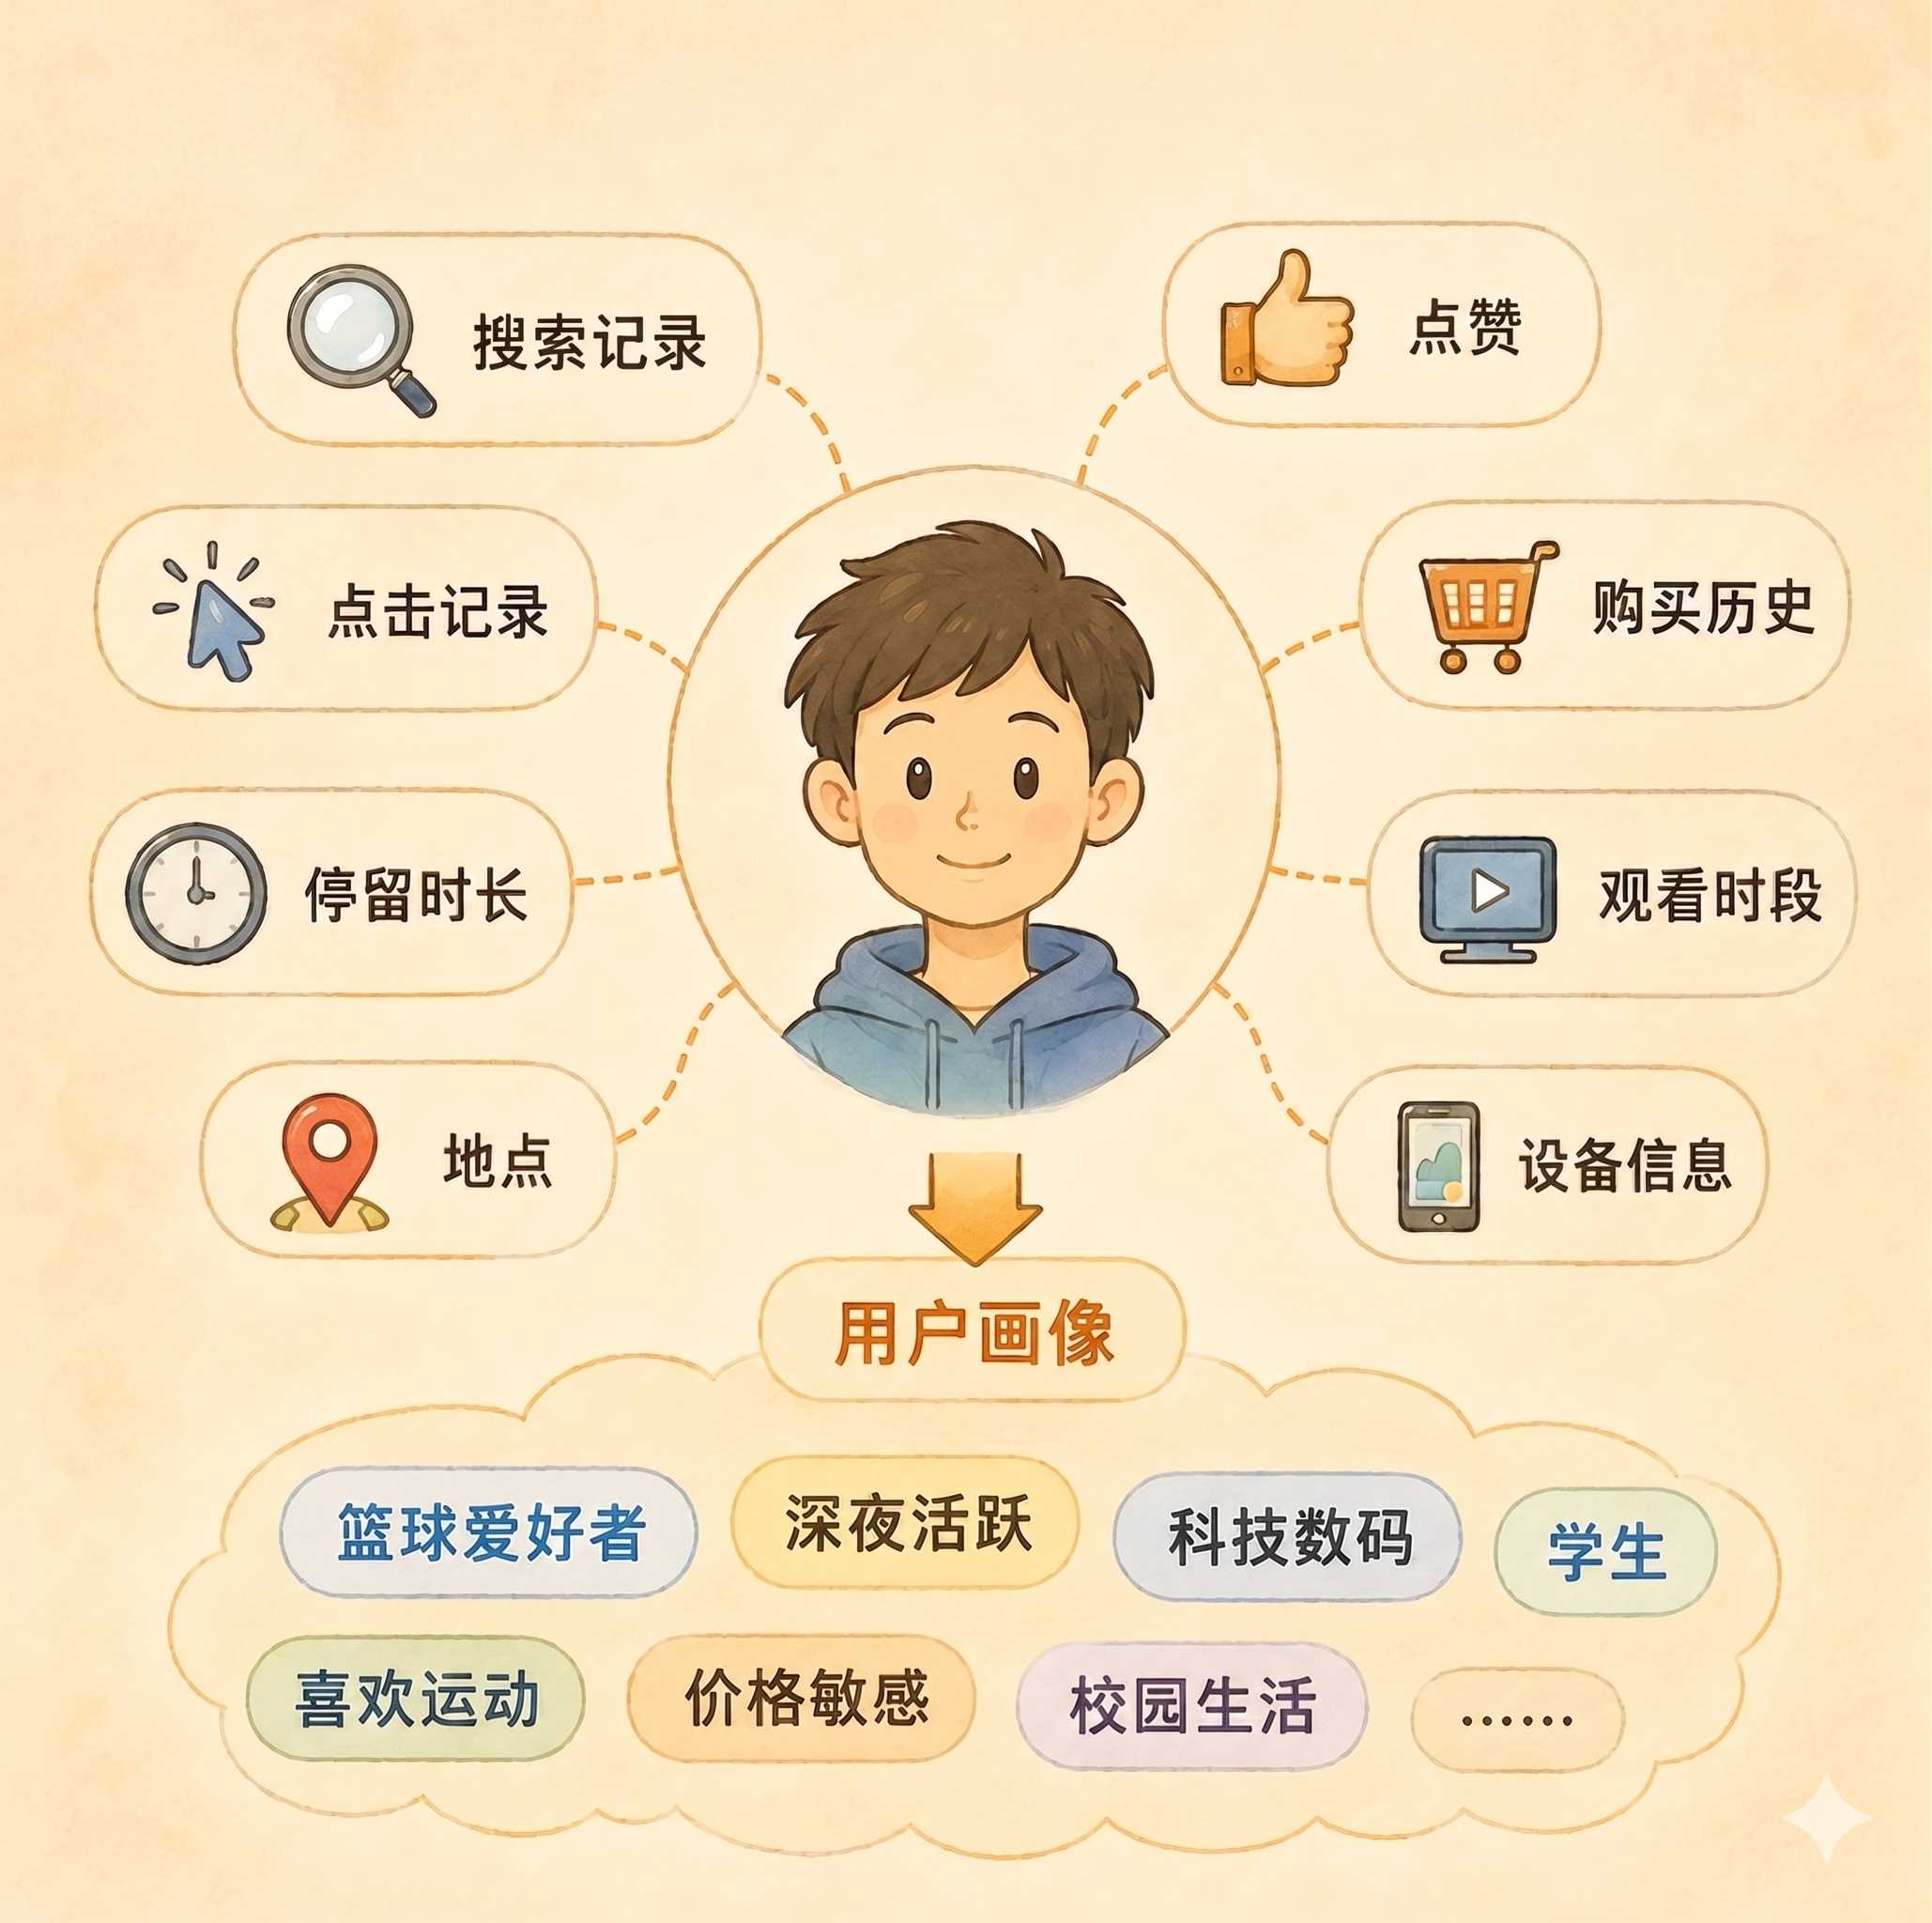
\includegraphics[width=0.88\textwidth]{images_chapter_01-03/2-2.png}
\caption*{\footnotesize\itshape\color{gray!50} 图2-2\quad 推荐系统如何从行为数据中“拼出”用户画像}
\end{figure}

这些行为数据是如何被AI使用的？平台记录的不是“小周喜欢篮球”，而是更具体、更原始的数据：他在某个视频上停留了3分28秒（全长3分30秒），看完后又手动回拖到第45秒重看了一遍慢动作回放。他点赞了三段类似视频中的两段，划走了另一段——因为那段是足球。

对于AI来说，这些行为组合在一起，几乎等于小周在大声喊：“我对篮球非常感兴趣！”

\textbf{一个有趣的真相：你其实是“免费的数据标注员”}

2016年，谷歌推出过一个叫“Quick, Draw!”的小游戏。规则很简单：你需要在20秒内画出一个指定物体（比如自行车、房子、长颈鹿），AI需要在20秒内猜出你画的是什么。这个游戏看起来可爱无害，但它帮谷歌收集了超过5000万张手绘涂鸦。这些涂鸦后来被用来训练AI理解人类如何画画——不是从照片中识别物体，而是从歪歪扭扭的简笔画中理解人类的表达方式。

你和朋友们在玩这个游戏的时候，其实是在免费帮谷歌训练AI。同样，你每一次点赞、每一次停留、每一次滑动屏幕，都在“告诉”AI：这个我喜欢，那个我没兴趣。你不是在“被AI观察”，你是在“帮AI变得更了解你”。

那么问题来了：这些看似零碎的行为碎片，到底是怎么被拼成一幅关于“你”的完整画像的？AI到底从这些数据中“学”到了什么？

\subsection{手机为什么总能“猜中”你的喜好}

让我们继续追踪小周的故事。

小周仔细回忆了自己这几天的行为：他没有搜索过“篮球”，没有关注篮球博主，也没有在篮球视频下留言。他做的唯一一件事，是那条NBA集锦视频他完整看完了，还反复看了几遍。

就凭这个？是的，就凭这个。

这里有一个很多人没意识到的关键：\textbf{“看了什么”比“说了什么”更重要。} 我们的嘴巴会说谎（“我要好好学习”），但手指很诚实——它诚实地在萌宠视频上停留了四十分钟。

平台收集到用户行为数据后，会进行一系列处理。不是某一条数据单独起作用，而是多种行为数据综合在一起形成判断。你看了什么内容、停留了多久、有没有点开评论区、看完整内容还是中途划走、看完之后有没有搜索相关内容、在什么时间段打开App——每一条单独看都说明不了什么，但组合在一起就极有信息量。AI不用理解“喜欢”这种情感是什么，它只需要知道：当“观看完成率超过95\%”和“主动回拖重看”和“接下来几天持续打开App”这三个行为同时出现时，把同类内容推到用户面前几乎一定是对的。

“用户画像”这个概念听起来很新，但它的底层逻辑其实比互联网还要古老。早在1940年代，美国社会学家就在做类似的事——通过分析人们的年龄、职业、居住地，来预测人们会买什么东西、投给哪个政客。只不过那时候靠的是问卷调查和人口统计，现在靠的是你手指的每一次滑动。

AI的“猜你喜欢”，本质和百货商场把化妆品放在一楼、把男装放在三楼是同一个逻辑：通过观察大量人的行为，总结出规律，然后预测下一个人的需求。AI唯一的不同是它能观察的人数远超任何一个人类——它能同时“记住”几亿人的所有行为，并从中找到人类根本无法靠手工发现的关联。

既然AI这么擅长发现规律，那它具体是怎么“学”的？这就要讲到现代人工智能最核心的技术——\textbf{机器学习}。

\subsection{机器学习——像教小孩一样教AI}

如果你要教一个两岁的小孩认识猫，你会怎么做？你不会让他读《猫科动物解剖学》，也不会给他讲“猫属于哺乳纲食肉目猫科”。你只会不断给他看猫的图片、带他去看邻居家的猫、指着街上的猫说“猫咪”。一开始他可能会把狗也认成猫。没关系，你纠正几次：这个不是猫，是狗狗。那个也不是猫，是兔兔。慢慢地，他就学会了。

\textbf{机器学习的基本逻辑，和这个过程几乎一模一样。}

\begin{figure}[H]
\centering
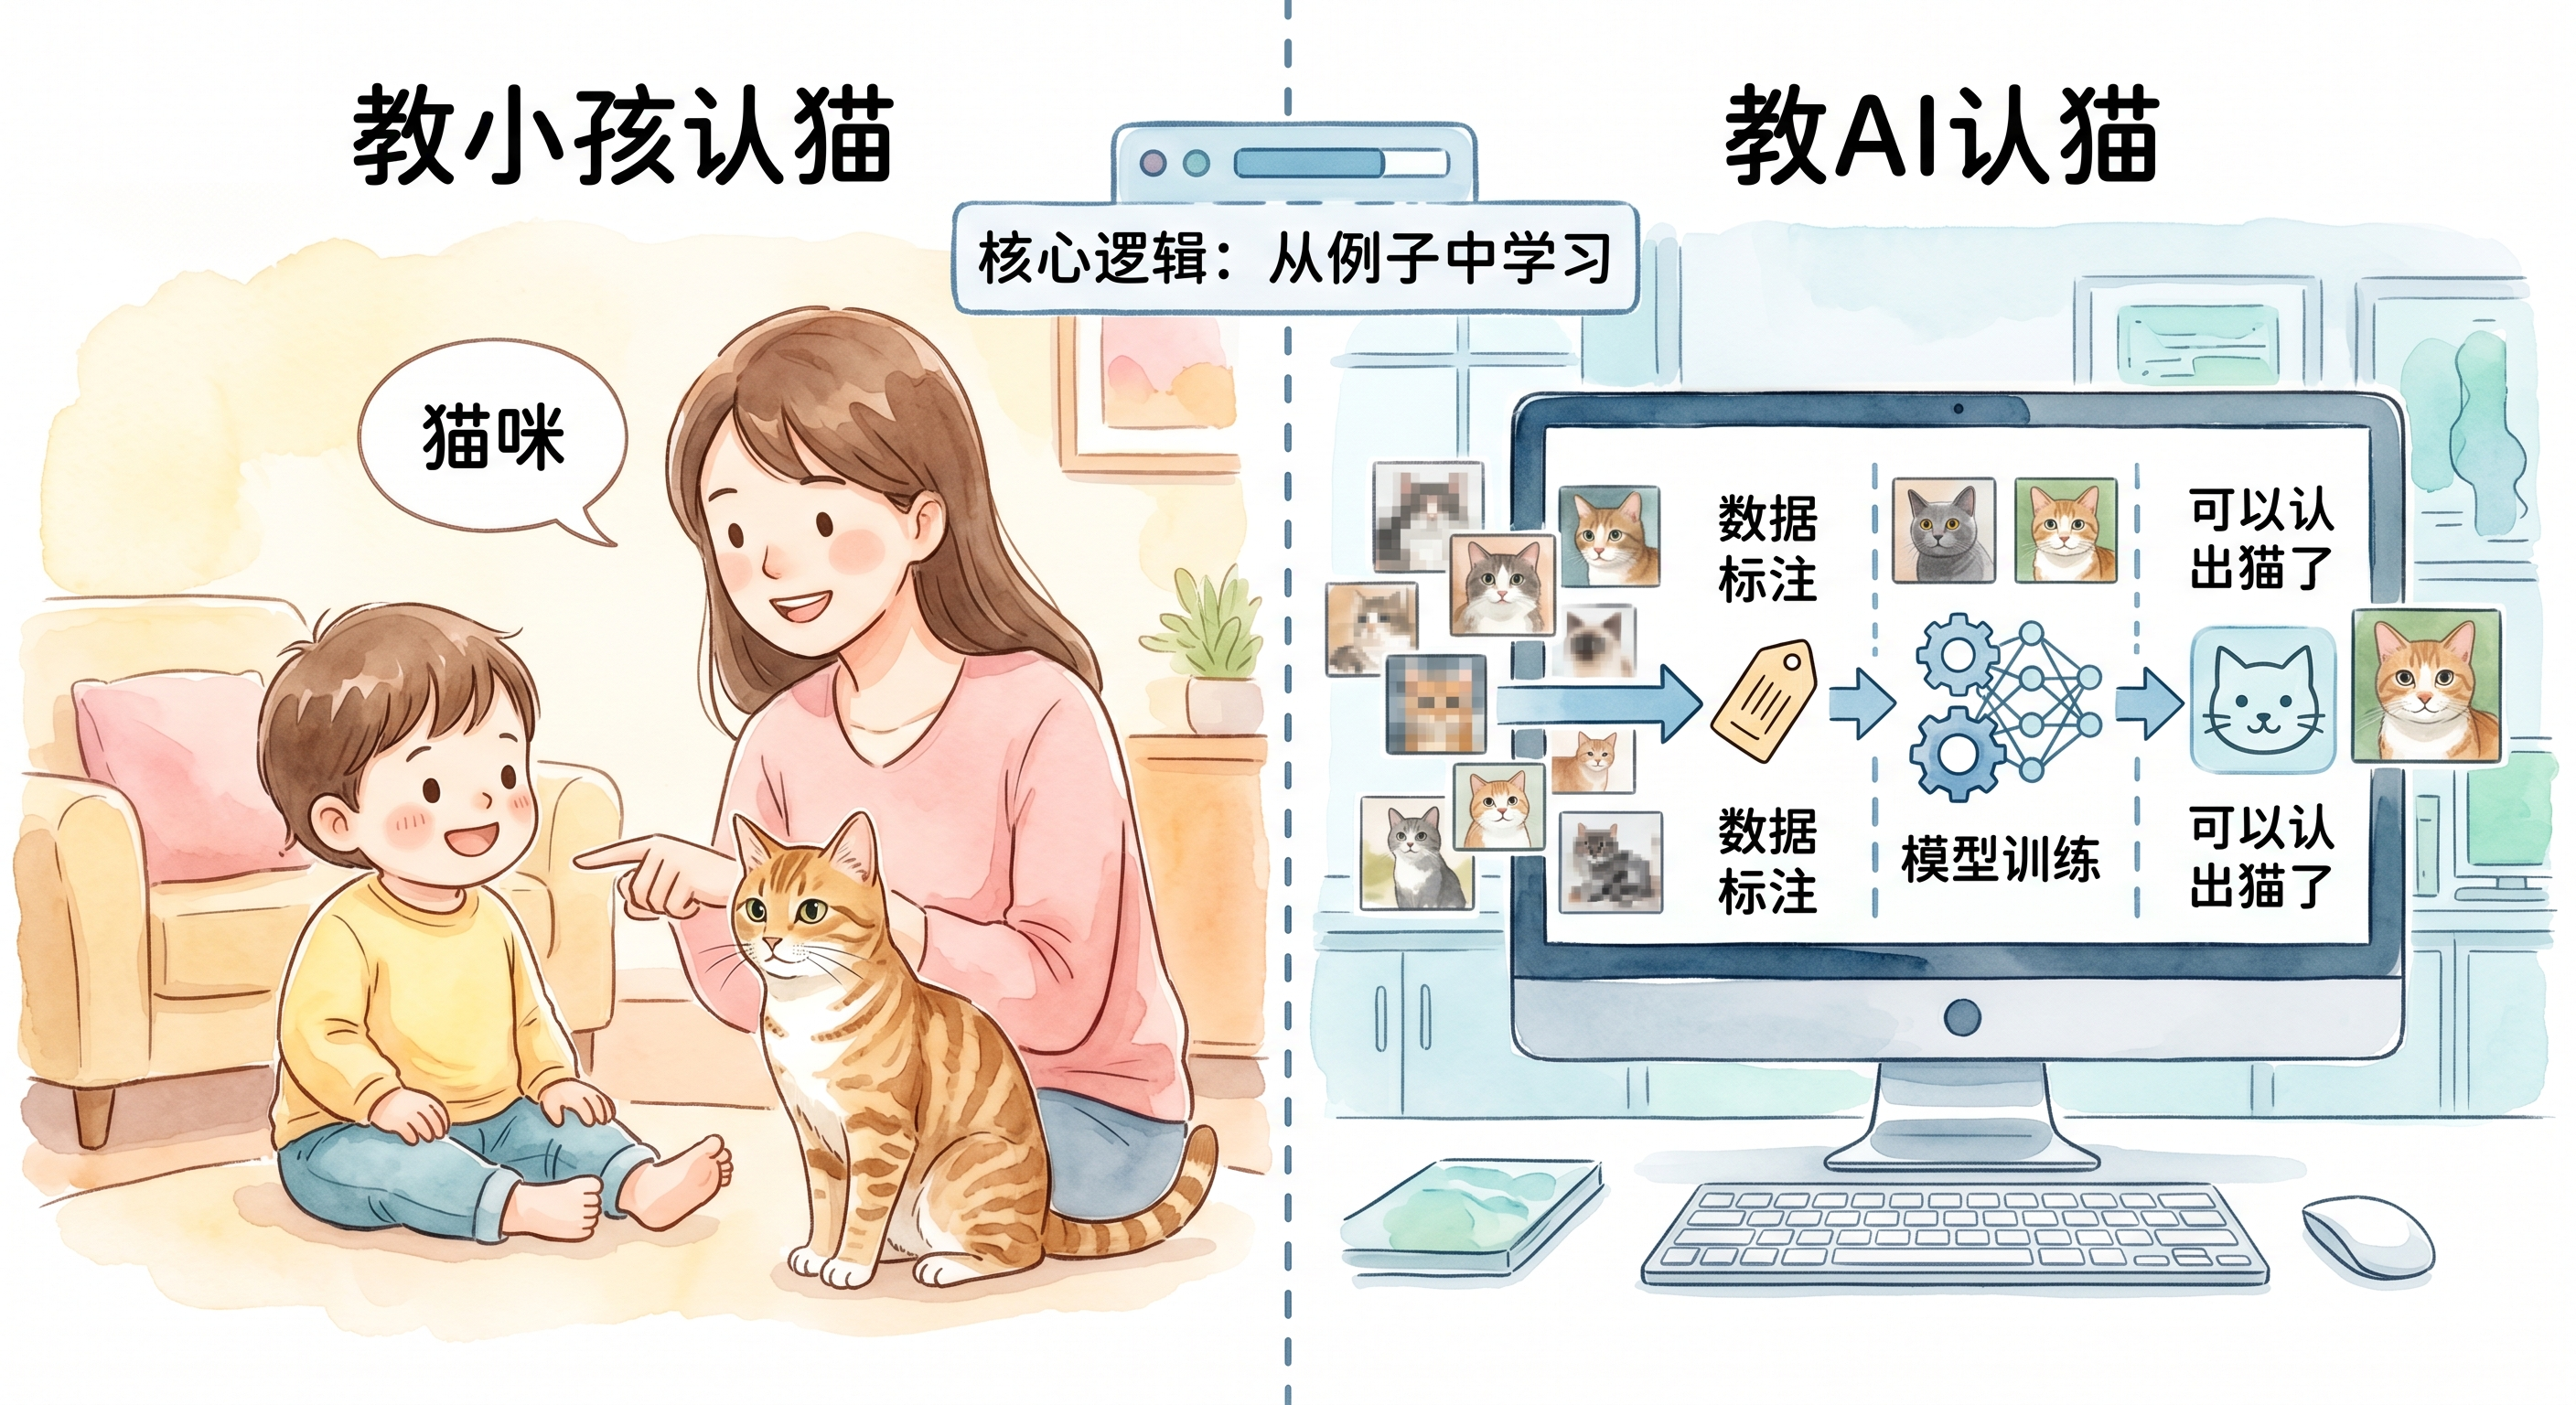
\includegraphics[width=0.88\textwidth]{images_chapter_01-03/2-3.png}
\caption*{\footnotesize\itshape\color{gray!50} 图2-3\quad 推荐系统如何从行为数据中“拼出”用户画像}
\end{figure}

传统的计算机程序，是靠人工编写规则来运行的。如果你想写一个“识别猫”的传统程序，你得一条条写规则：“如果这个动物有四条腿、尖耳朵、长胡须、会喵喵叫，那就是猫。”但问题来了——有些猫耳朵是垂下来的，有些猫胡须不明显，斯芬克斯无毛猫全身光溜溜的。规则永远写不完，例外永远存在。

机器学习换了一种思路：\textbf{不给AI写规则，给它看成千上万个例子，让它自己找规律。}

这个过程可以用学生最熟悉的场景来类比——刷题。你不会把每道题的标准答案背下来，数学题千变万化，你背不完。你是通过刷大量题目来总结“这类题应该怎么解”的规律。AI也一样。给它“投喂”海量标注好的数据——这叫\textbf{数据集}。AI从中提取特征、总结规律、不断修正错误，最终形成稳定的判断能力。这个过程叫\textbf{模型训练}。训练完成的AI就像一个刷了十万道题的学生，再遇到类似的问题，就能给出比较准确的判断。

\begin{figure}[H]
\centering
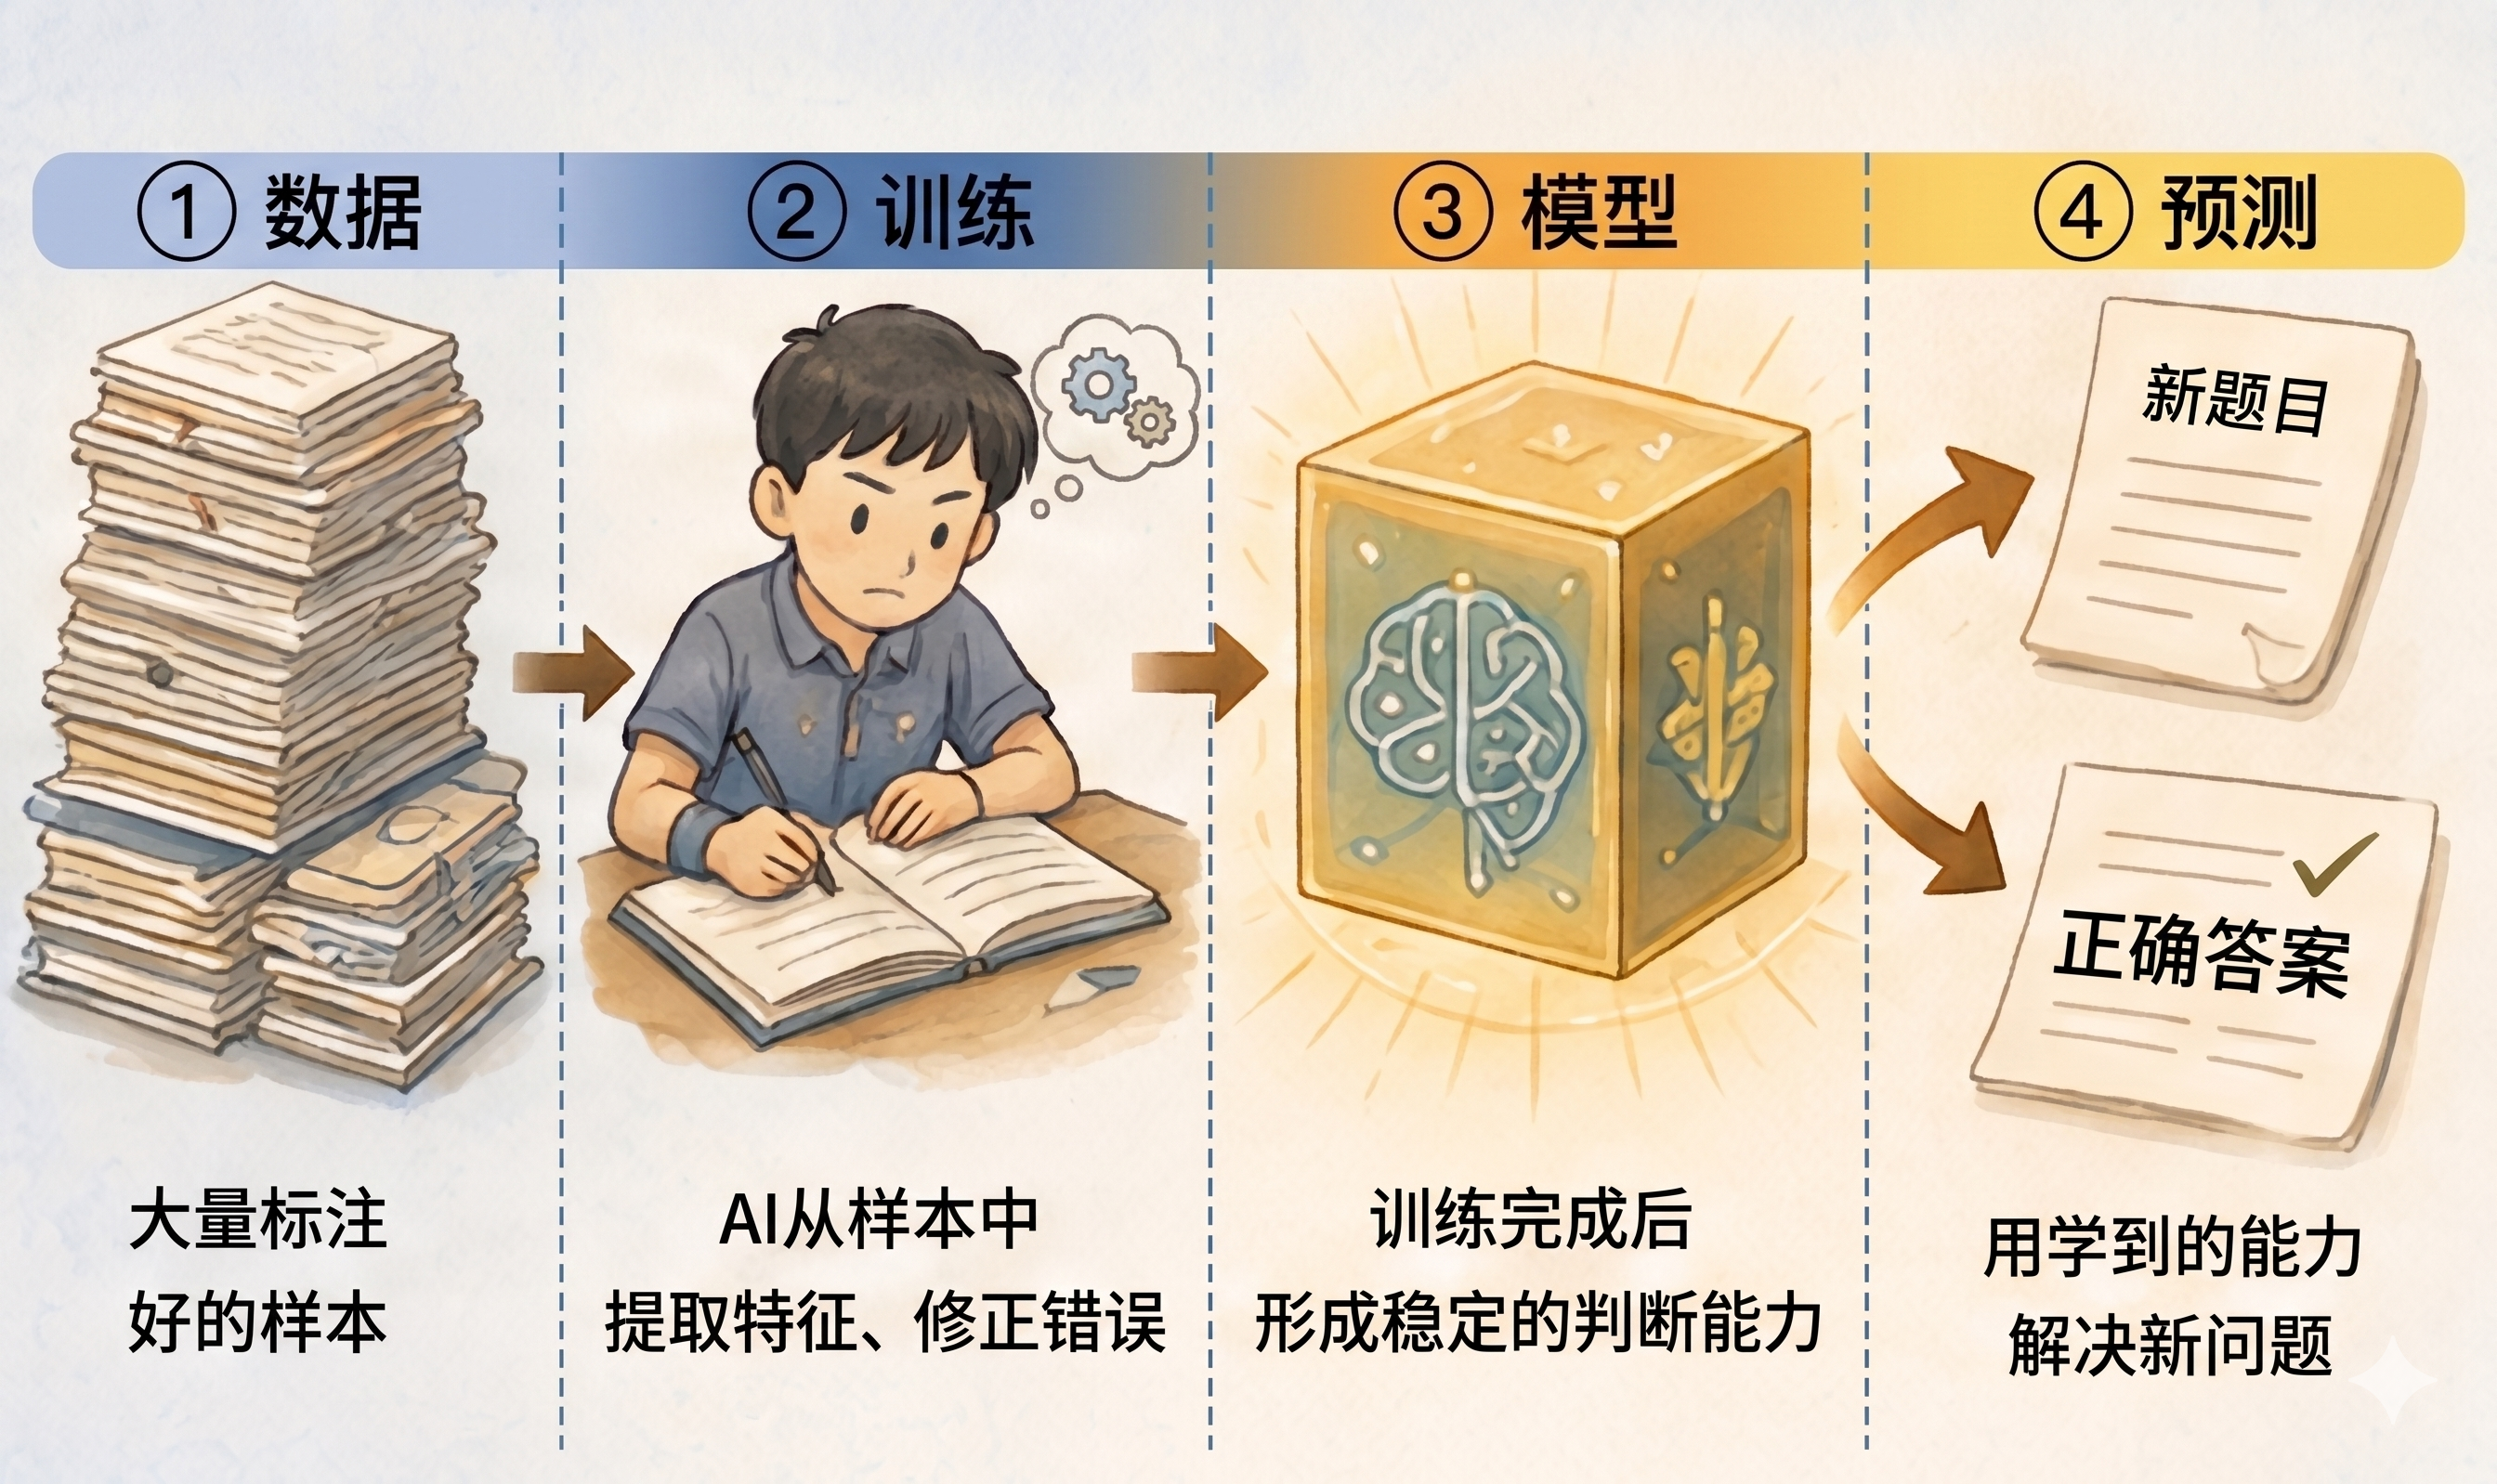
\includegraphics[width=0.88\textwidth]{images_chapter_01-03/2-4.png}
\caption*{\footnotesize\itshape\color{gray!50} 图2-4\quad 推荐系统如何从行为数据中“拼出”用户画像}
\end{figure}

这个过程中最关键的是什么？\textbf{数据。} AI的能力上限，很大程度上取决于“投喂”给它的数据质量。如果训练数据里猫的照片都是在白天拍的，AI在晚上可能就认不出猫了。如果数据里大多是橘猫，AI面对黑猫时可能会犹豫。如果数据本身带有偏见——比如“医生”的图片大多是男性——AI就会学到这个偏见并忠实地复制它。

\begin{knowledgebox}
\textbf{数据集与数据标注——AI的“教材”与“标准答案”}

想象你要教一个从没见过猫的外星人认识猫。最好的办法就是给它看几百张猫的照片，每张照片背面写上“这是猫”。这些照片就是\textbf{数据集}——用来训练AI的样本集合。照片背面的文字就是\textbf{数据标注}——给训练样本贴上正确答案的标签。标注通常由人工完成，非常耗时耗力。但标注质量直接决定AI学得好不好——标注错了，AI就会学错。AI领域因此流行一句玩笑话：“AI的智能，其实是被一群按件计酬的数据标注员‘喂’出来的。”
\end{knowledgebox}

机器学习是本章所有后续内容的基础。接下来你会看到，计算机视觉是机器学习在图像上的应用，自然语言处理是机器学习在文本上的应用，生成式AI是机器学习从“识别”向“创造”的进阶。它们共享同一个底层逻辑：\textbf{从数据中学习规律，然后用规律来预测未知。}

那么，机器学习到底能在现实生活中做什么？只是认猫认狗和推荐视频吗？

\begin{funbox}
\textbf{谷歌大脑的“猫脸”实验——AI自己“发现”了猫}

2012年，谷歌大脑（Google Brain）的研究者做了一个当时看来有些“疯狂”的实验。他们用16000个计算机处理器组成了一个庞大的神经网络，然后让它“看”了1000万张从YouTube视频中随机截取的图片。他们没有告诉AI任何关于这些图片的知识——没有标注“这是猫”“这是人脸”“这是一辆自行车”。他们只是让AI自己去看。

训练结束后，研究者检查了这个神经网络的内部状态。一个令人震惊的发现浮出水面：在这个完全自学、无人指导的过程中，AI自发地“进化”出了一个对“猫脸”高度敏感的神经元。它不知道“猫”这个词，没见过“猫科动物”的定义，但它从1000万张图片的统计规律中自己“发现”了：这种圆脸、尖耳朵、长胡须的物体在图片中反复出现，一定是某种重要的存在。

这个故事最迷人的地方在于：AI的学习方式，某种程度上与婴儿认识世界的方式有相似之处——不需要被告知“这是什么”，只需要看到足够多的例子，就能自己总结出规律。
\end{funbox}

\subsection{机器学习应用案例}

机器学习已经渗透到我们生活的各个角落。在学习领域，它帮你自动批改作文、推荐适合你水平的练习题；在安全领域，它识别诈骗短信和异常交易；在交通领域，它预测路况和优化导航路线；在气象领域，它分析卫星云图预测天气；在医学领域，它辅助医生发现早期病灶；在商业领域，它分析用户行为精准推荐商品。从你手机里的输入法到天上的气象卫星，从医院的CT机到电商平台的推荐引擎——机器学习的应用广度远超大多数人的想象。

下面，我们通过三个具体案例，看看这项技术是如何在不同领域真实运作的。

\subsubsection*{案例1：诈骗短信为什么会被自动拦截}

晚上十一点，大一学生小李的手机突然震了一下。他迷迷糊糊拿起手机，屏幕上的短信预览让他瞬间清醒：“【快递通知】您的包裹因地址填写错误已被退回，请立即点击链接重新确认，否则24小时后将自动销毁。”短信里快递公司的名称、客服电话、页面格式，都和真的一模一样。小李确实有两个快递在路上，他手指已经悬在了链接上方。

就在这时，手机顶部弹出一行灰色小字：“⚠️ 疑似诈骗短信，已被系统自动拦截至垃圾箱。”

小李长舒一口气。但他随即产生了一个疑问：机器到底是怎么知道这是一条诈骗短信的？

它并不像人类一样“看懂”了这条短信的内容。它不知道什么叫“欺骗”，什么叫“利用人的焦虑心理”。它只是在海量历史数据中，寻找诈骗短信的共同模式。当被举报过的诈骗短信积累到百万级、千万级时，某些规律就自然浮现了：诈骗短信里大量出现“包裹退回”“地址错误”“立即点击”“自动销毁”这类制造紧迫感的关键词组合；链接通常是不明短链接或仿冒域名；发送号码往往是虚拟号段或境外号码；发送行为也很特别——短时间内大规模群发，不像普通人发短信的节奏。

正常短信完全不是这个画风：快递通知告知取件码和驿站地址，语气平稳；银行短信包含具体金额和卡号尾号，不会让你点不明链接。

AI通过对比海量的“诈骗短信”和“正常短信”，逐渐学会了一套判断规则。它做的其实是一个概率计算：“综合来看，这条短信像诈骗短信的概率有多高？”当概率超过99\%时，直接拦截；当概率在60\%左右时，标记为“疑似”放进垃圾箱，等你手动确认。

这个案例的核心启示是：AI并不“懂诈骗”，它只是在做模式识别——从海量数据中总结重复出现的规律。而这，正是机器学习最核心的能力。

\begin{figure}[H]
\centering

\includegraphics[width=0.88\textwidth]{images_chapter_01-03/2-4b.png}
\caption*{\footnotesize\itshape\color{gray!50} 图2-4b\quad 推荐系统如何从行为数据中“拼出”用户画像}
\end{figure}

\subsubsection*{案例2：输入法是怎么“猜”到你要打的字}

你每天都在用输入法打字，但你可能注意过这样一个细节：当你打出“我今天想去”这几个字后，输入法会自动在候选栏里推荐“学校”“食堂”“图书馆”“超市”这些词。它怎么知道你想说什么？

输入法背后的AI系统，通过分析海量用户的打字数据来学习语言规律。它记录的不是“某个具体的人在打什么字”，而是“某个词后面最常跟着什么词”。比如“想去”这个词，在海量数据中后面跟着“学校”的概率是15\%，跟着“食堂”的概率是12\%，跟着“图书馆”的概率是8\%。当你打出“我今天想去”时，AI就根据这个统计规律，把最可能的后接词推送到候选栏的前排。

更有趣的是，输入法还能学习你个人的打字习惯。如果你是一个经常打“我想去打篮球”的人，AI就会在你的个人模型里把“篮球”的权重调高。下次你再打“我想去”，它会在候选栏更靠前的位置显示“打篮球”。这就是为什么用同一款输入法的人，推荐的词却各不相同——AI已经悄悄“摸透”了你的表达习惯。

这个案例的核心启示是：AI不“懂”语言，它只是通过海量数据中的词频统计和搭配规律，计算出最可能的下一个词。你每一次打字，都在帮AI变得更“了解”你的表达方式。

\begin{knowledgebox}
\textbf{语言模型——AI的“词语接龙”高手}

输入法背后使用的技术，在AI领域被称为\textbf{语言模型}。你可以把它想象成一个玩“词语接龙”的超级高手。它读遍了人类写过的几乎所有文本，记住了“高兴”后面常跟着“快乐”，“天气”后面常跟着“晴朗”。当你输入“今天天气”，它的大脑（其实是一个巨大的概率表）立刻浮现出“真好”“晴朗”“糟糕”等选项，并挑出最可能的那一个推荐给你。它不知道这些词的意思，但比任何人都更熟悉它们之间的搭配关系。
\end{knowledgebox}

\subsubsection*{案例3：AI如何预测天气}

“明天局部地区有雨”——这句天气预报的背后，是AI对海量气象数据的分析。

气象卫星每天从地球各个角落传回温度、湿度、气压、风速、云层厚度等数据，数据量以TB计。人类预报员不可能在短时间内处理完这么多信息。而机器学习模型可以——它“吃”进过去几十年的历史气象数据，从中学习天气变化的规律：某个区域的气压下降3百帕通常意味着什么？海洋表面温度升高1度会对台风路径产生什么影响？各种气象要素之间有什么复杂的非线性关系？

通过这些学习，AI能对未来几小时到未来两周的天气做出预测。虽然天气预报偶尔还是不准——因为天气系统是极端复杂的混沌系统，微小变化都可能引发巨大的预测偏差——但相比几十年前纯靠人工经验和简单物理模型的时代，AI让预报准确率大大提升。今天，AI甚至可以预测某个具体位置的“未来两小时降雨量”——精确到分钟级和百米级，帮你决定“现在出门要不要带伞”。

这个案例的核心启示是：机器学习的本质，是让AI从历史数据中总结规律，然后用这些规律来预判未知事件。从拦截诈骗短信到预测天气，从猜你想打的字到辅助诊断疾病，这项技术已经渗透到生活的方方面面。

\begin{knowledgebox}
\textbf{混沌系统——一只蝴蝶引发龙卷风}

天气预报之所以偶尔失灵，根子在于天气是一个典型的\textbf{混沌系统}。混沌系统最著名的比喻是“蝴蝶效应”：一只蝴蝶在巴西扇动翅膀，可能引发德克萨斯的一场龙卷风。因为系统对初始条件极其敏感，任何微小的测量误差，都会在预测中被迅速放大。所以，天气预报达不到100\%准确，这不是AI的错，而是天气本身那难以捉摸的本性。
\end{knowledgebox}

\subsection{AI真的会“思考”吗}

先讲一个有点好笑的真实经历。小周买过一双篮球鞋。买完之后，他连续三天都在购物App的首页看到更多篮球鞋推荐——不同品牌、不同配色、不同价位，全都是篮球鞋。问题在于：\textbf{他已经买过了。}

一个正常人类店员不会在你刚刚买了一双鞋走出店门后追出来喊：“先生先生！您可能还对这双鞋感兴趣！”但AI会。因为它并不理解“买过了”和“还没买”的区别。它只知道你最近对篮球鞋表现出很强的兴趣——非常强——所以继续推荐。

这就是AI的第一个局限：\textbf{没有常识。} AI知道的是数据告诉它的东西：你看了篮球鞋，篮球鞋和运动相关，所以推更多篮球鞋。但它不理解“人一般不会短时间内买两双同类型的鞋”这个常识。

如果你仔细观察，会发现AI类似的“没常识”行为比比皆是：天气预报说“明天降雨概率80\%”，结果第二天艳阳高照——因为天气系统极端复杂，AI只能基于历史数据做概率推测。AI客服反复问你“请再说一遍您的问题”，因为它没有真正理解你的意图，只是在做关键词匹配。

这是AI的第二个局限：\textbf{没有情感。} AI不知道什么叫“喜欢”。当它给你推荐一首歌的时候，不是因为这首歌触动过它，而是因为它计算出你和这首歌之间存在某种数据关联——你和喜欢这首歌的其他用户有相似的行为模式，或者这首歌的节奏特征和你常听的歌很接近。

这是AI的第三个、也是最根本的局限：\textbf{没有意识。} AI不知道“我正在做判断”。当你问它“今天天气怎么样”时，它调取气象数据给出回答——整个过程里，没有任何一个步骤是“它在想”。它只是在运行一套数学运算。它不会在给出天气预报后心想“希望明天别下雨，我还要打球呢”。它不在乎天气。它什么都不在乎。

所以，回到本节标题的问题：\textbf{AI真的会“思考”吗？}

答案很明确：\textbf{不会。} AI只是在做概率判断。它从海量数据中总结规律，然后用这些规律来预测未知。这种能力看起来像“思考”，但本质上只是统计学意义上的模式匹配。它没有常识、没有情感、没有意识——它是在“计算”，不是在“思考”。

\begin{figure}[H]
\centering
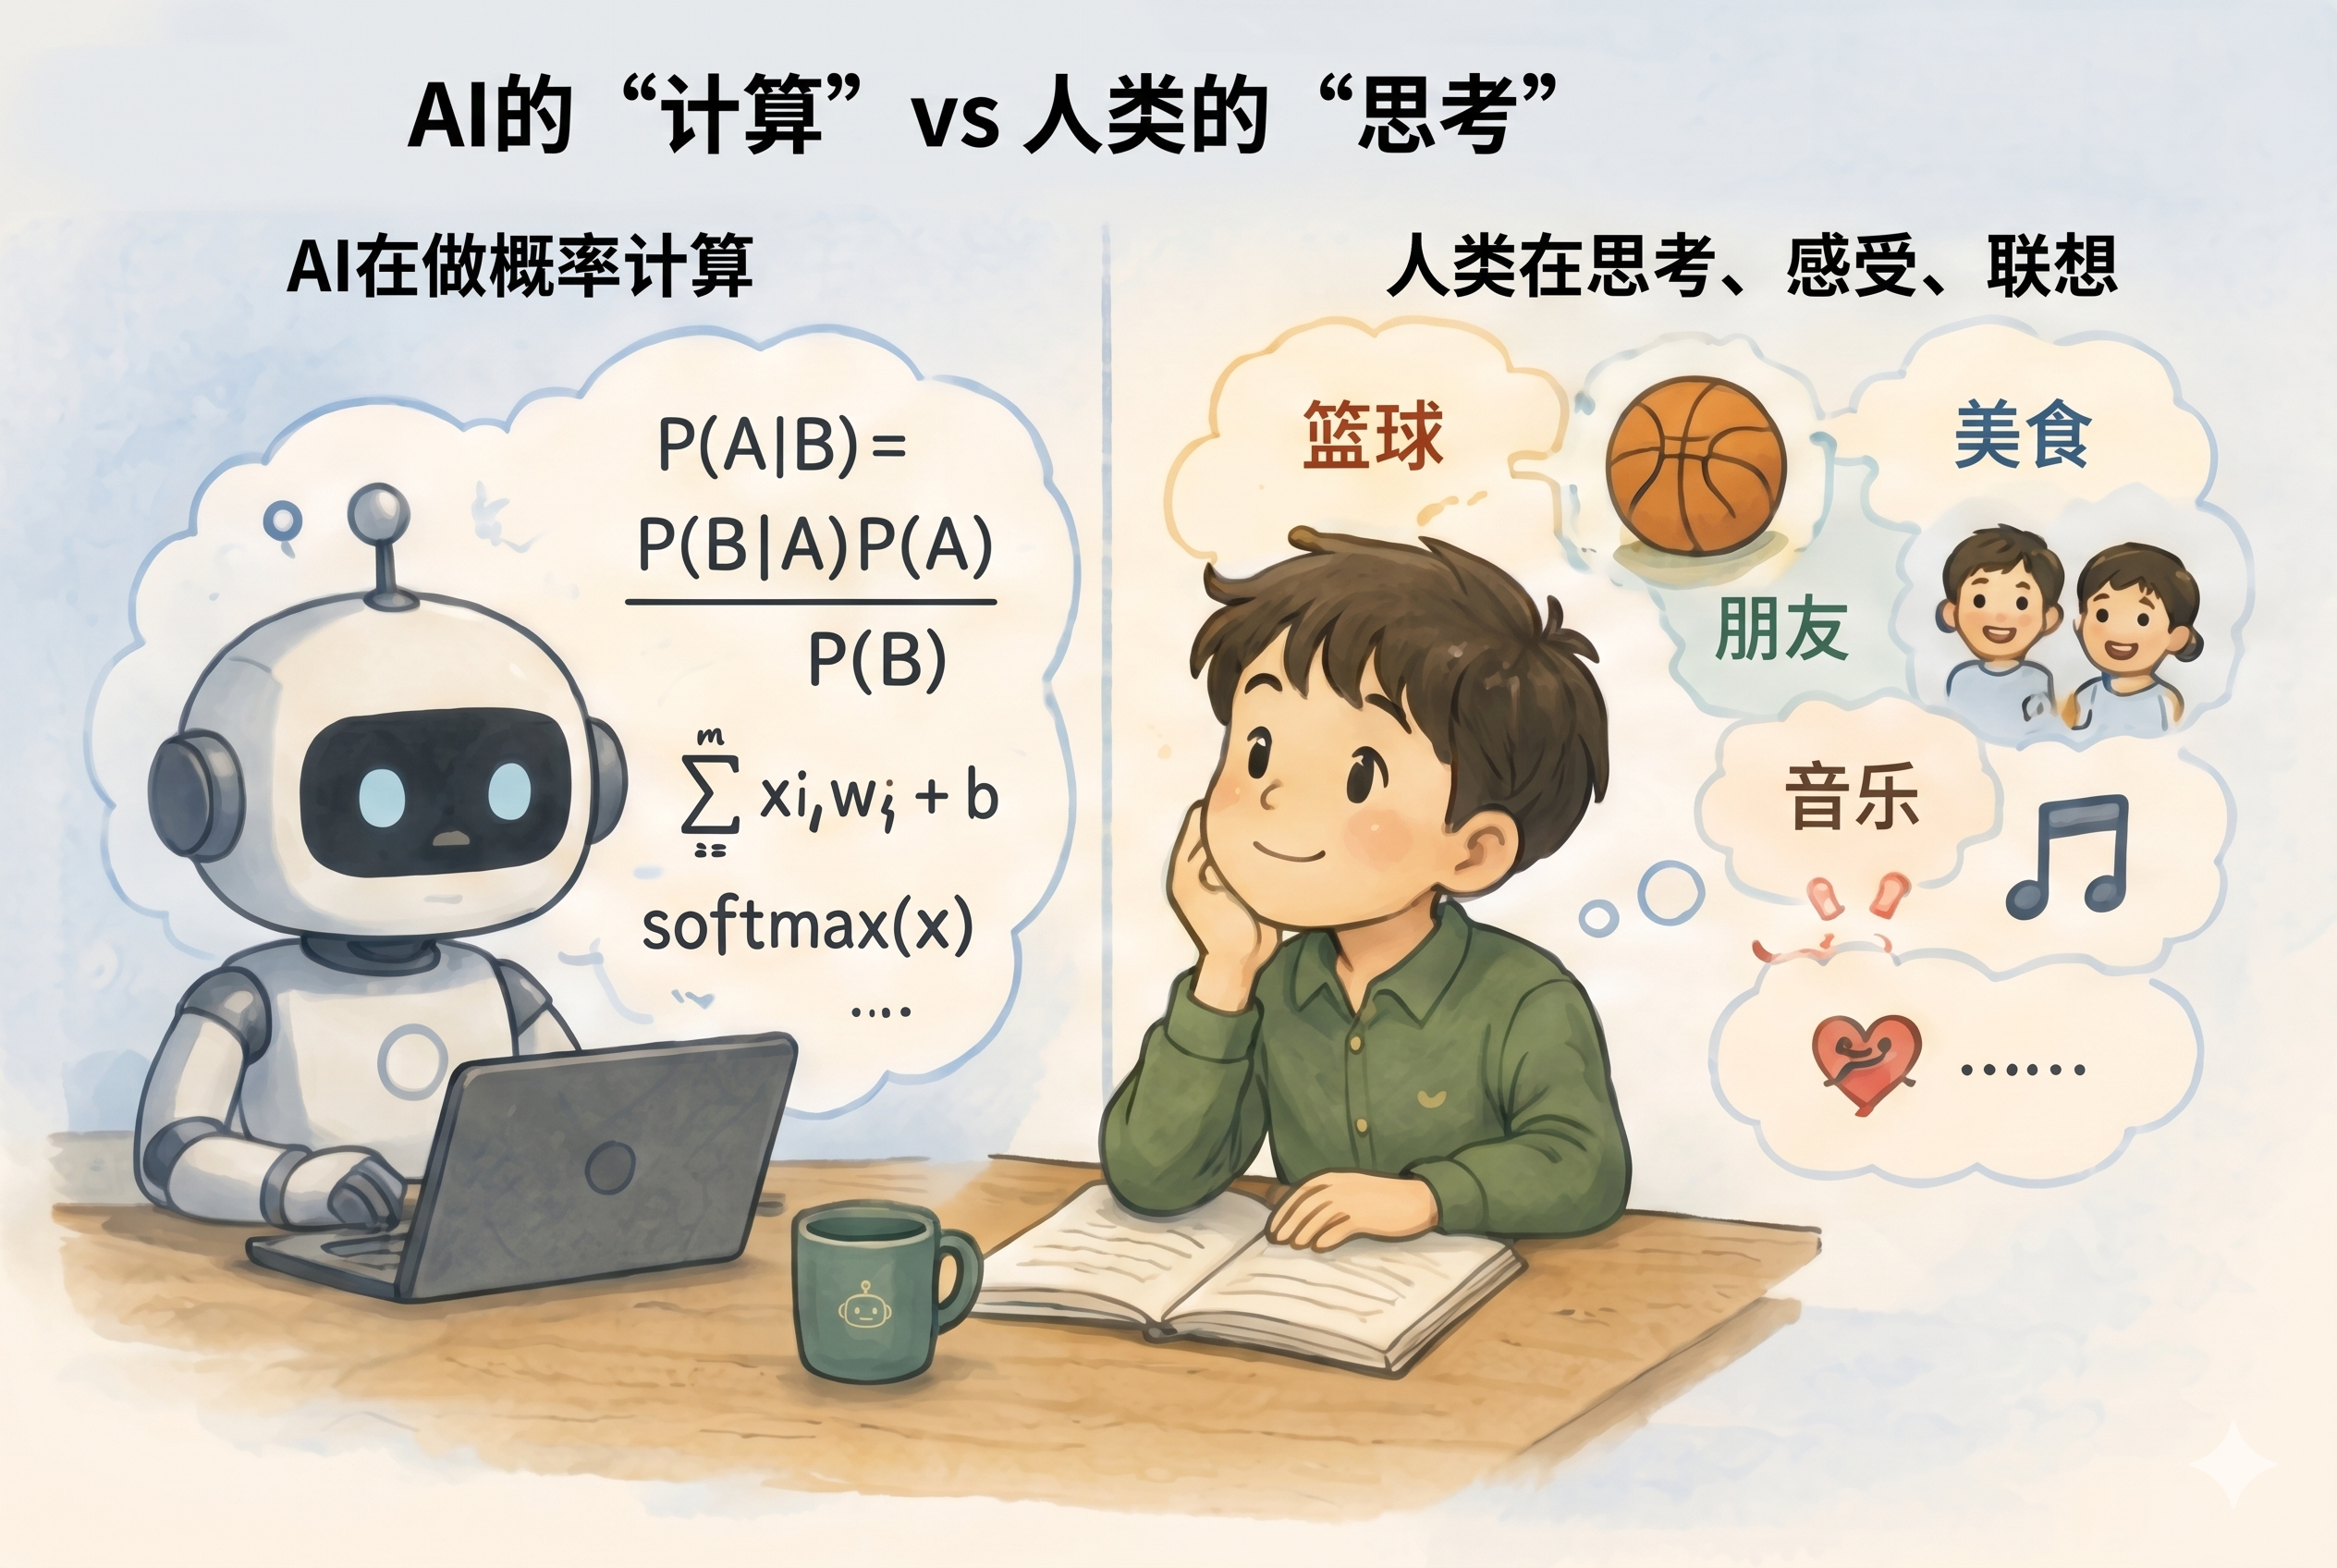
\includegraphics[width=0.88\textwidth]{images_chapter_01-03/2-5.png}
\caption*{\footnotesize\itshape\color{gray!50} 图2-5\quad 推荐系统如何从行为数据中“拼出”用户画像}
\end{figure}

理解这一点非常重要。理解了AI不会思考，你就不会对它产生不必要的恐惧——担心它哪天突然“觉醒”取代人类；你也不会对它产生不切实际的崇拜——以为它什么都知道、什么都懂。AI是工具。一个极其擅长发现规律、但完全不知道自己在做什么的工具。

接下来，我们要看看AI如何把这种“发现规律”的能力应用到视觉领域——如何从像素中“看见”世界。

\section{计算机视觉：AI学会“看见”世界}

上一节我们讲了AI如何从数据中学习规律。现在，让我们看看AI怎样把这种“学习”能力应用到视觉上——让机器“看见”世界。

2012年，一个名叫AlexNet的AI模型在ImageNet图像识别竞赛中震惊了学界。这个模型由当时还是研究生的亚历克斯·克里泽夫斯基（Alex Krizhevsky）和他的导师杰弗里·辛顿（Geoffrey Hinton）共同设计。他们用两块游戏显卡（NVIDIA GTX 580）训练了一个深度神经网络，结果在识别图片物体的比赛中，错误率从前一年的约26\%骤降至约16\%——这个巨大的飞跃令整个计算机视觉领域为之震动。从那之后，计算机视觉进入了快车道。而你可能每天都在用这项技术，却从未意识到。

\subsection{身边到处都是“长了眼睛”的机器}

大三学生小语的一天，是被机器“看”着度过的。

早晨七点半，她匆匆走过校园门禁。摄像头捕捉到她的脸，系统在不到一秒内完成了“检测人脸→提取特征→比对数据库→确认身份→开门”的全流程。她不用掏校园卡，甚至不用停下脚步。这台刷脸门禁背后的AI，已经在过去三年里“看”过她上千次——大一刚入学时她戴眼镜、留刘海；大二换了隐形眼镜、剪了短发；大三开始化淡妆——但AI始终认得她。因为它存储的不是某张特定照片，而是一组不断更新的面部特征数据。

中午在食堂，她对着支付终端眨了个眼。机器确认“活体检测通过，身份验证成功”——它能区分面前是真人还是一张照片或一段视频。

晚上她躺在床上，掏出手机。前置红外摄像头投射出三万个不可见的光点，在她脸上形成一张深度地图。面容ID在一秒内匹配成功，屏幕解锁。她点开相册，发现AI已经自动把她今天拍的37张照片按人脸分好了组——室友一个文件夹、社团朋友一个文件夹、课堂板书一个文件夹。

\begin{figure}[H]
\centering
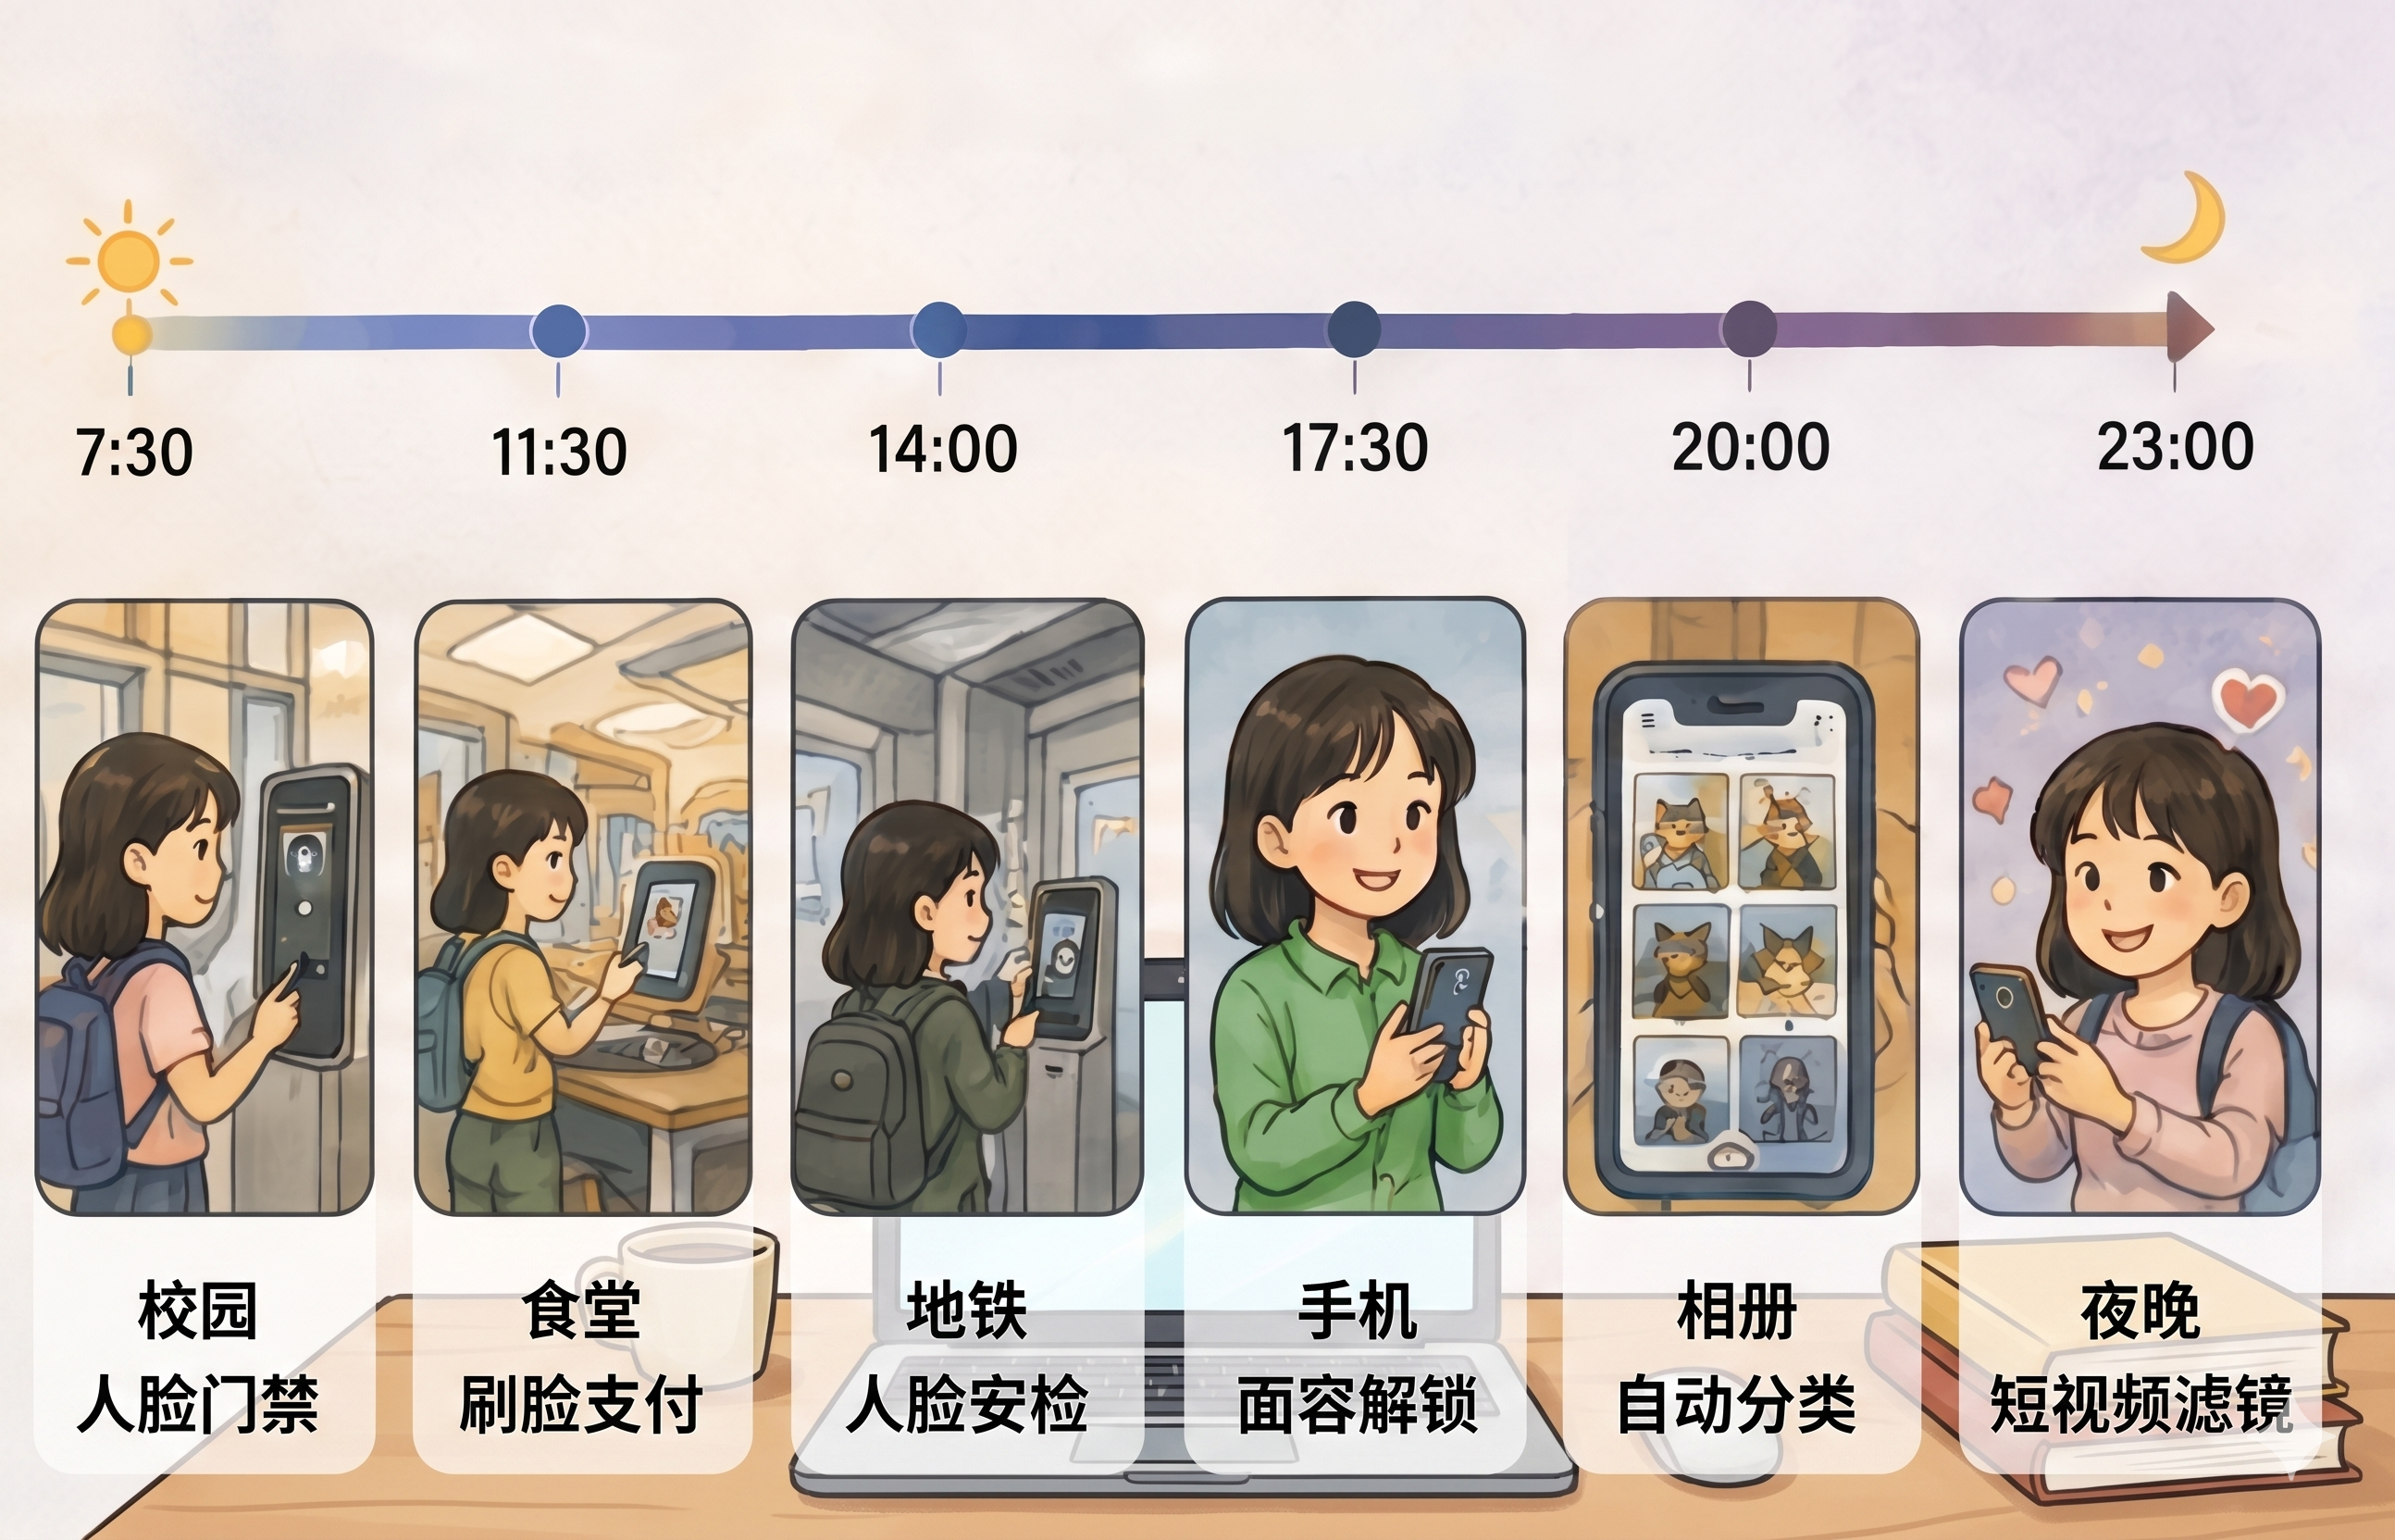
\includegraphics[width=0.88\textwidth]{images_chapter_01-03/2-6.png}
\caption*{\footnotesize\itshape\color{gray!50} 图2-6\quad 推荐系统如何从行为数据中“拼出”用户画像}
\end{figure}

这些只是小语能感知到的。在她看不见的地方，更多的“机器眼睛”正在工作：医院放射科，AI正在初筛今天的第200份CT影像，一个微小的肺结节被自动圈出并标注了坐标和风险等级；她暑假实习过的工厂流水线上，AI质检系统正以每秒几十个零件的速度扫描着产品外观，寻找纳米级别的表面瑕疵；城郊的农田上空，搭载AI摄像头的无人机正在分析作物叶片的光谱数据，判断哪一片田需要施肥、哪一片可能遭受了虫害。

那么问题来了：\textbf{一台由金属和硅片组成的机器，是怎么“看见”东西的？它看到的世界，和我们看到的一样吗？}

\subsection{人脸识别为什么有时会失败}

在回答“AI怎么看世界”之前，我们先从一个你可能也有过的困惑说起。

小语发现，白天解锁手机特别顺畅，但晚上关了灯之后，有时候怎么都解不开。戴了口罩之后，校门口的门禁偶尔认不出她。拍照时如果角度太偏，手机相册的人脸分类也会出错。

要理解这是为什么，你需要先理解一个根本性的差异：\textbf{人类“看”和AI“看”，是两件完全不同的事。}

当你看一张朋友的照片时，你的大脑自动完成了无数复杂处理——你认出了朋友的脸，感受到了他当时的情绪（开心还是尴尬），注意到了背景里的教学楼，甚至想起了那天一起吃饭的场景。你“看到”的是一个有意义的整体，你的大脑调用了你和这个人所有的交往记忆、你对人类表情的理解、你在这个世界生活了十几二十年的全部经验。

但AI面对这张照片时，它看到的只是一堆数字。一张高清照片在AI眼里是几百万个像素方格，每个像素有一个颜色数值。没有笑脸，没有回忆，没有阳光洒在桌上的温暖——只有数字。

\begin{figure}[H]
\centering
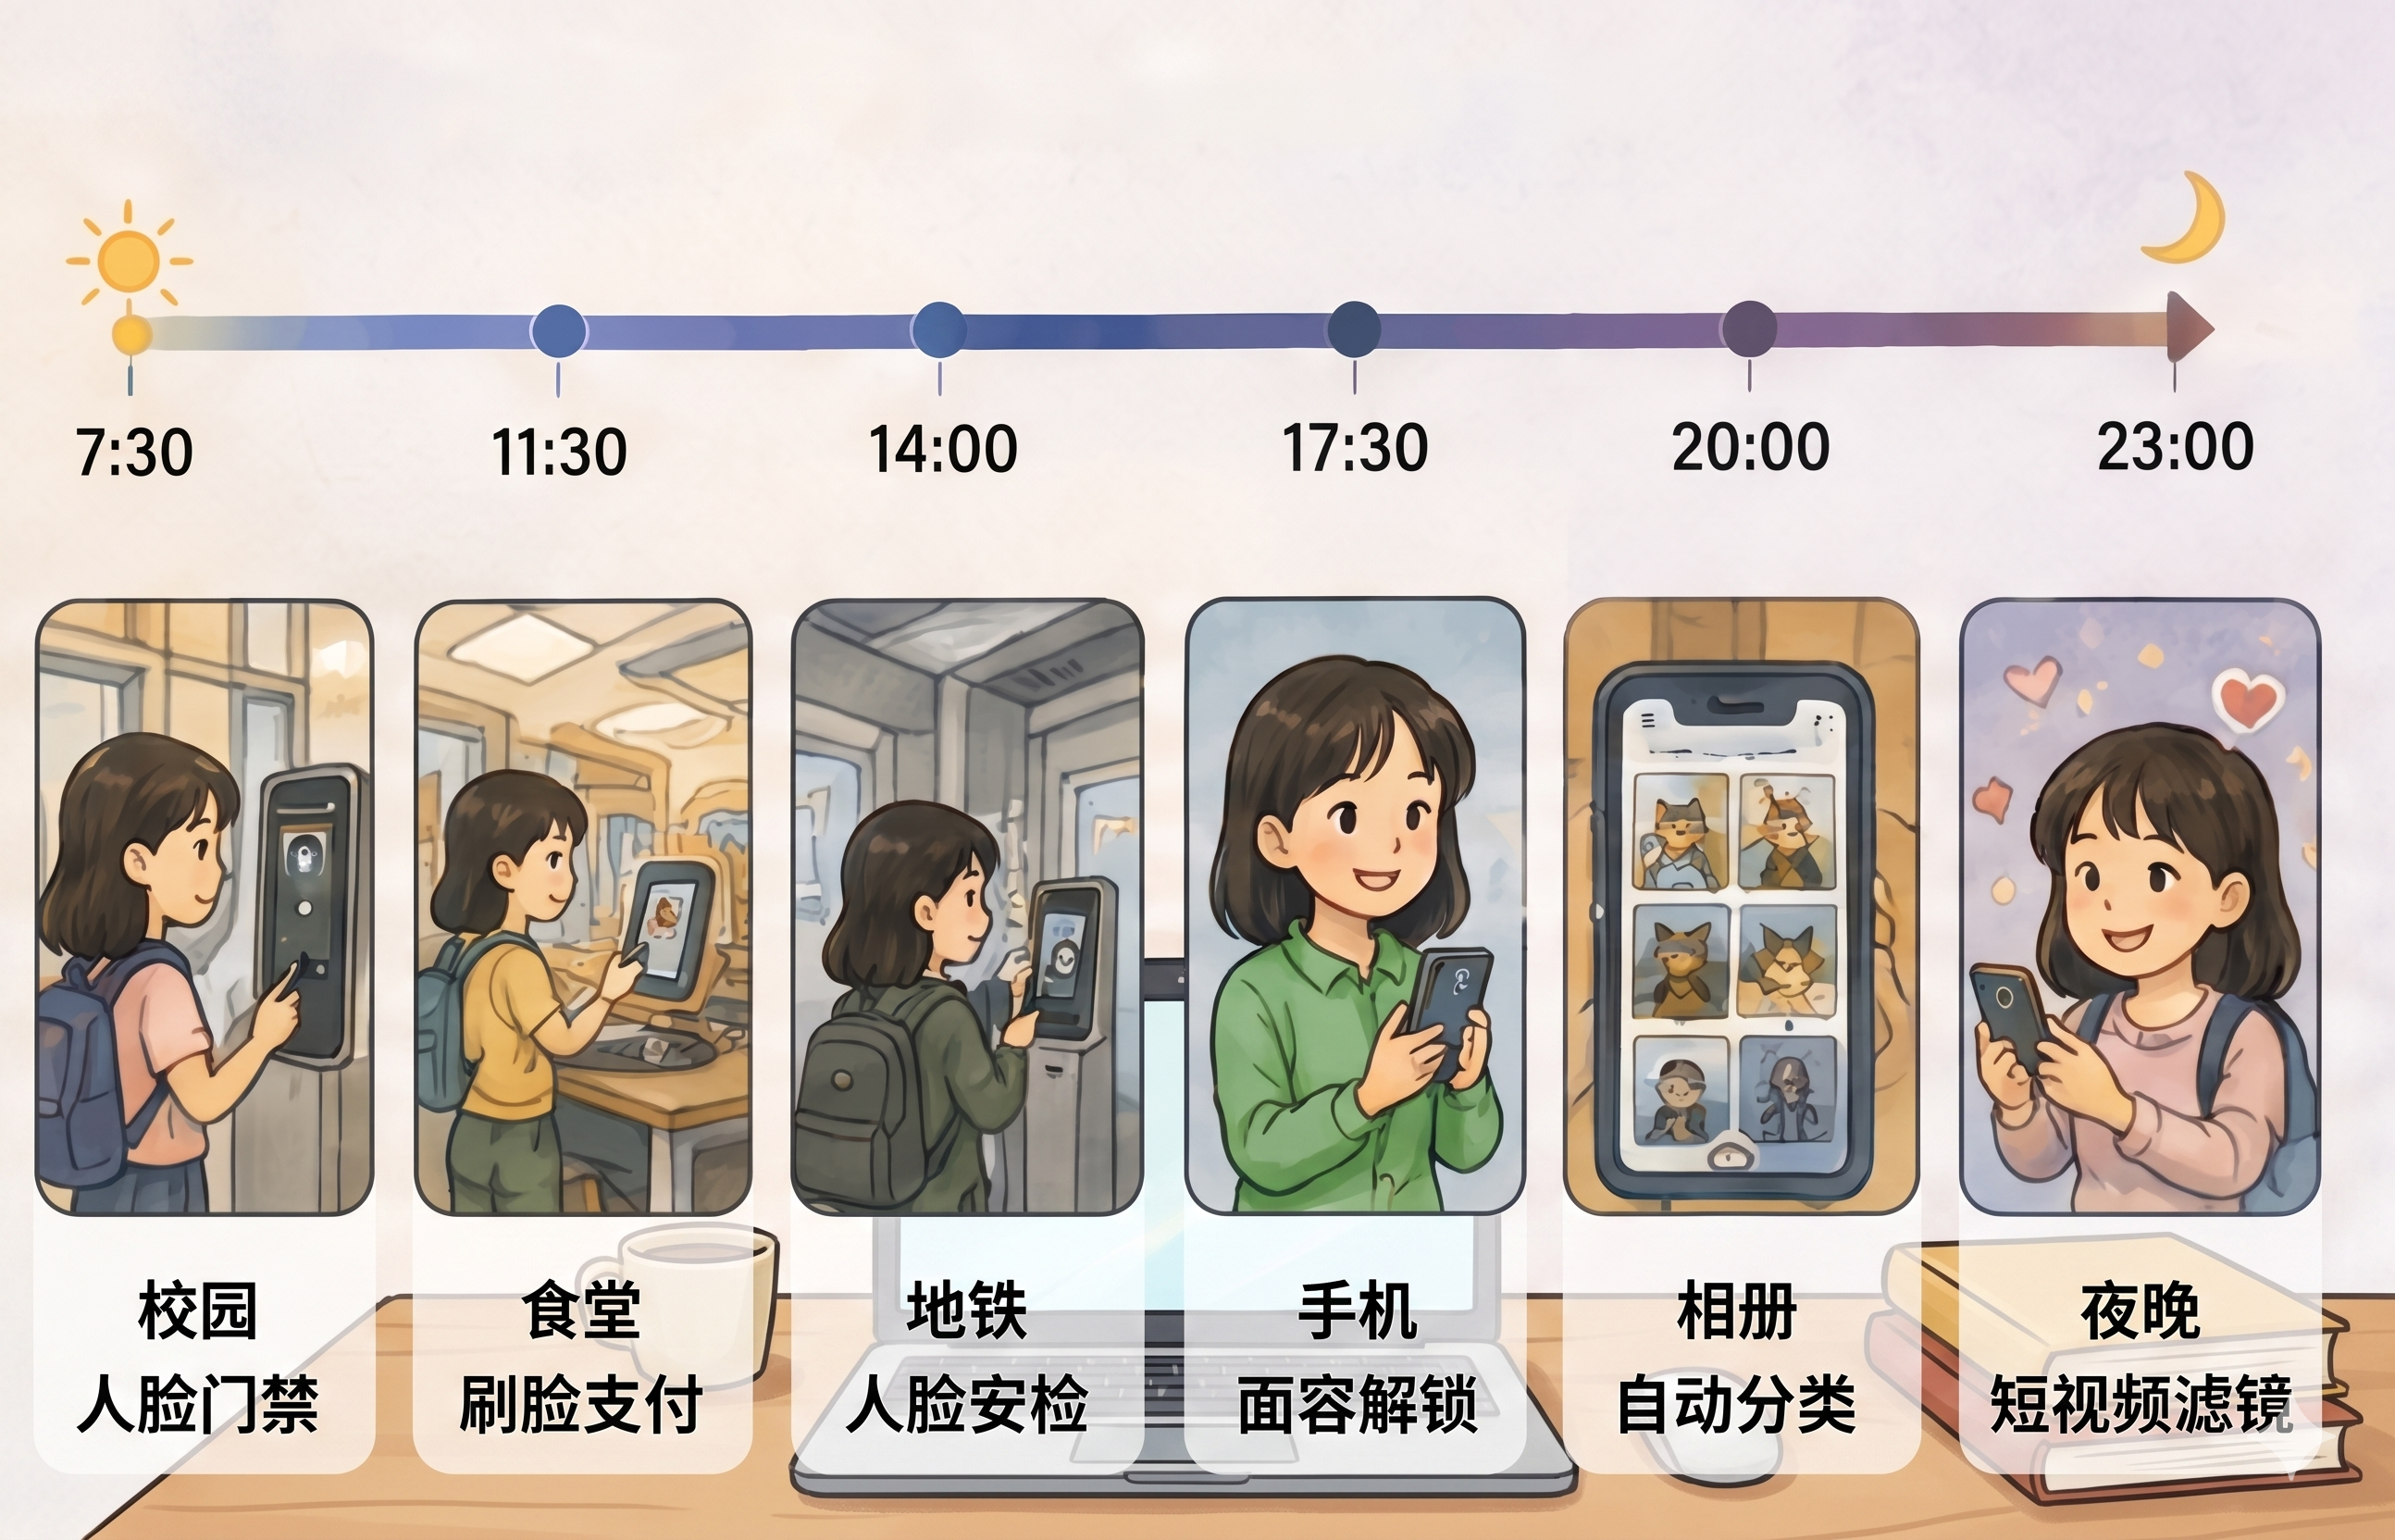
\includegraphics[width=0.88\textwidth]{images_chapter_01-03/2-6.png}
\caption*{\footnotesize\itshape\color{gray!50} 图2-2\quad 推荐系统如何从行为数据中“拼出”用户画像}
\end{figure}

AI需要从这堆数字里找规律：哪里是轮廓？哪里是边缘？颜色怎么分布？它通过分析成千上万张标注过的“人脸”图片，逐渐学会了：人脸通常有某些共同特征——两只眼睛之间大约是一个眼睛的宽度，鼻梁在脸部中间，嘴唇在鼻子下方一定距离。

现在你可以回答“为什么关灯就认不出来”了——因为黑暗中像素信息变少，AI提取到的特征不够清晰。戴口罩认不出来？因为口罩遮住了鼻子和嘴巴，AI少了一半的特征信息。角度太偏认不出来？因为AI训练时看到的大多是正面照片，侧面和仰角的样本较少，特征匹配困难。

\begin{figure}[H]
\centering
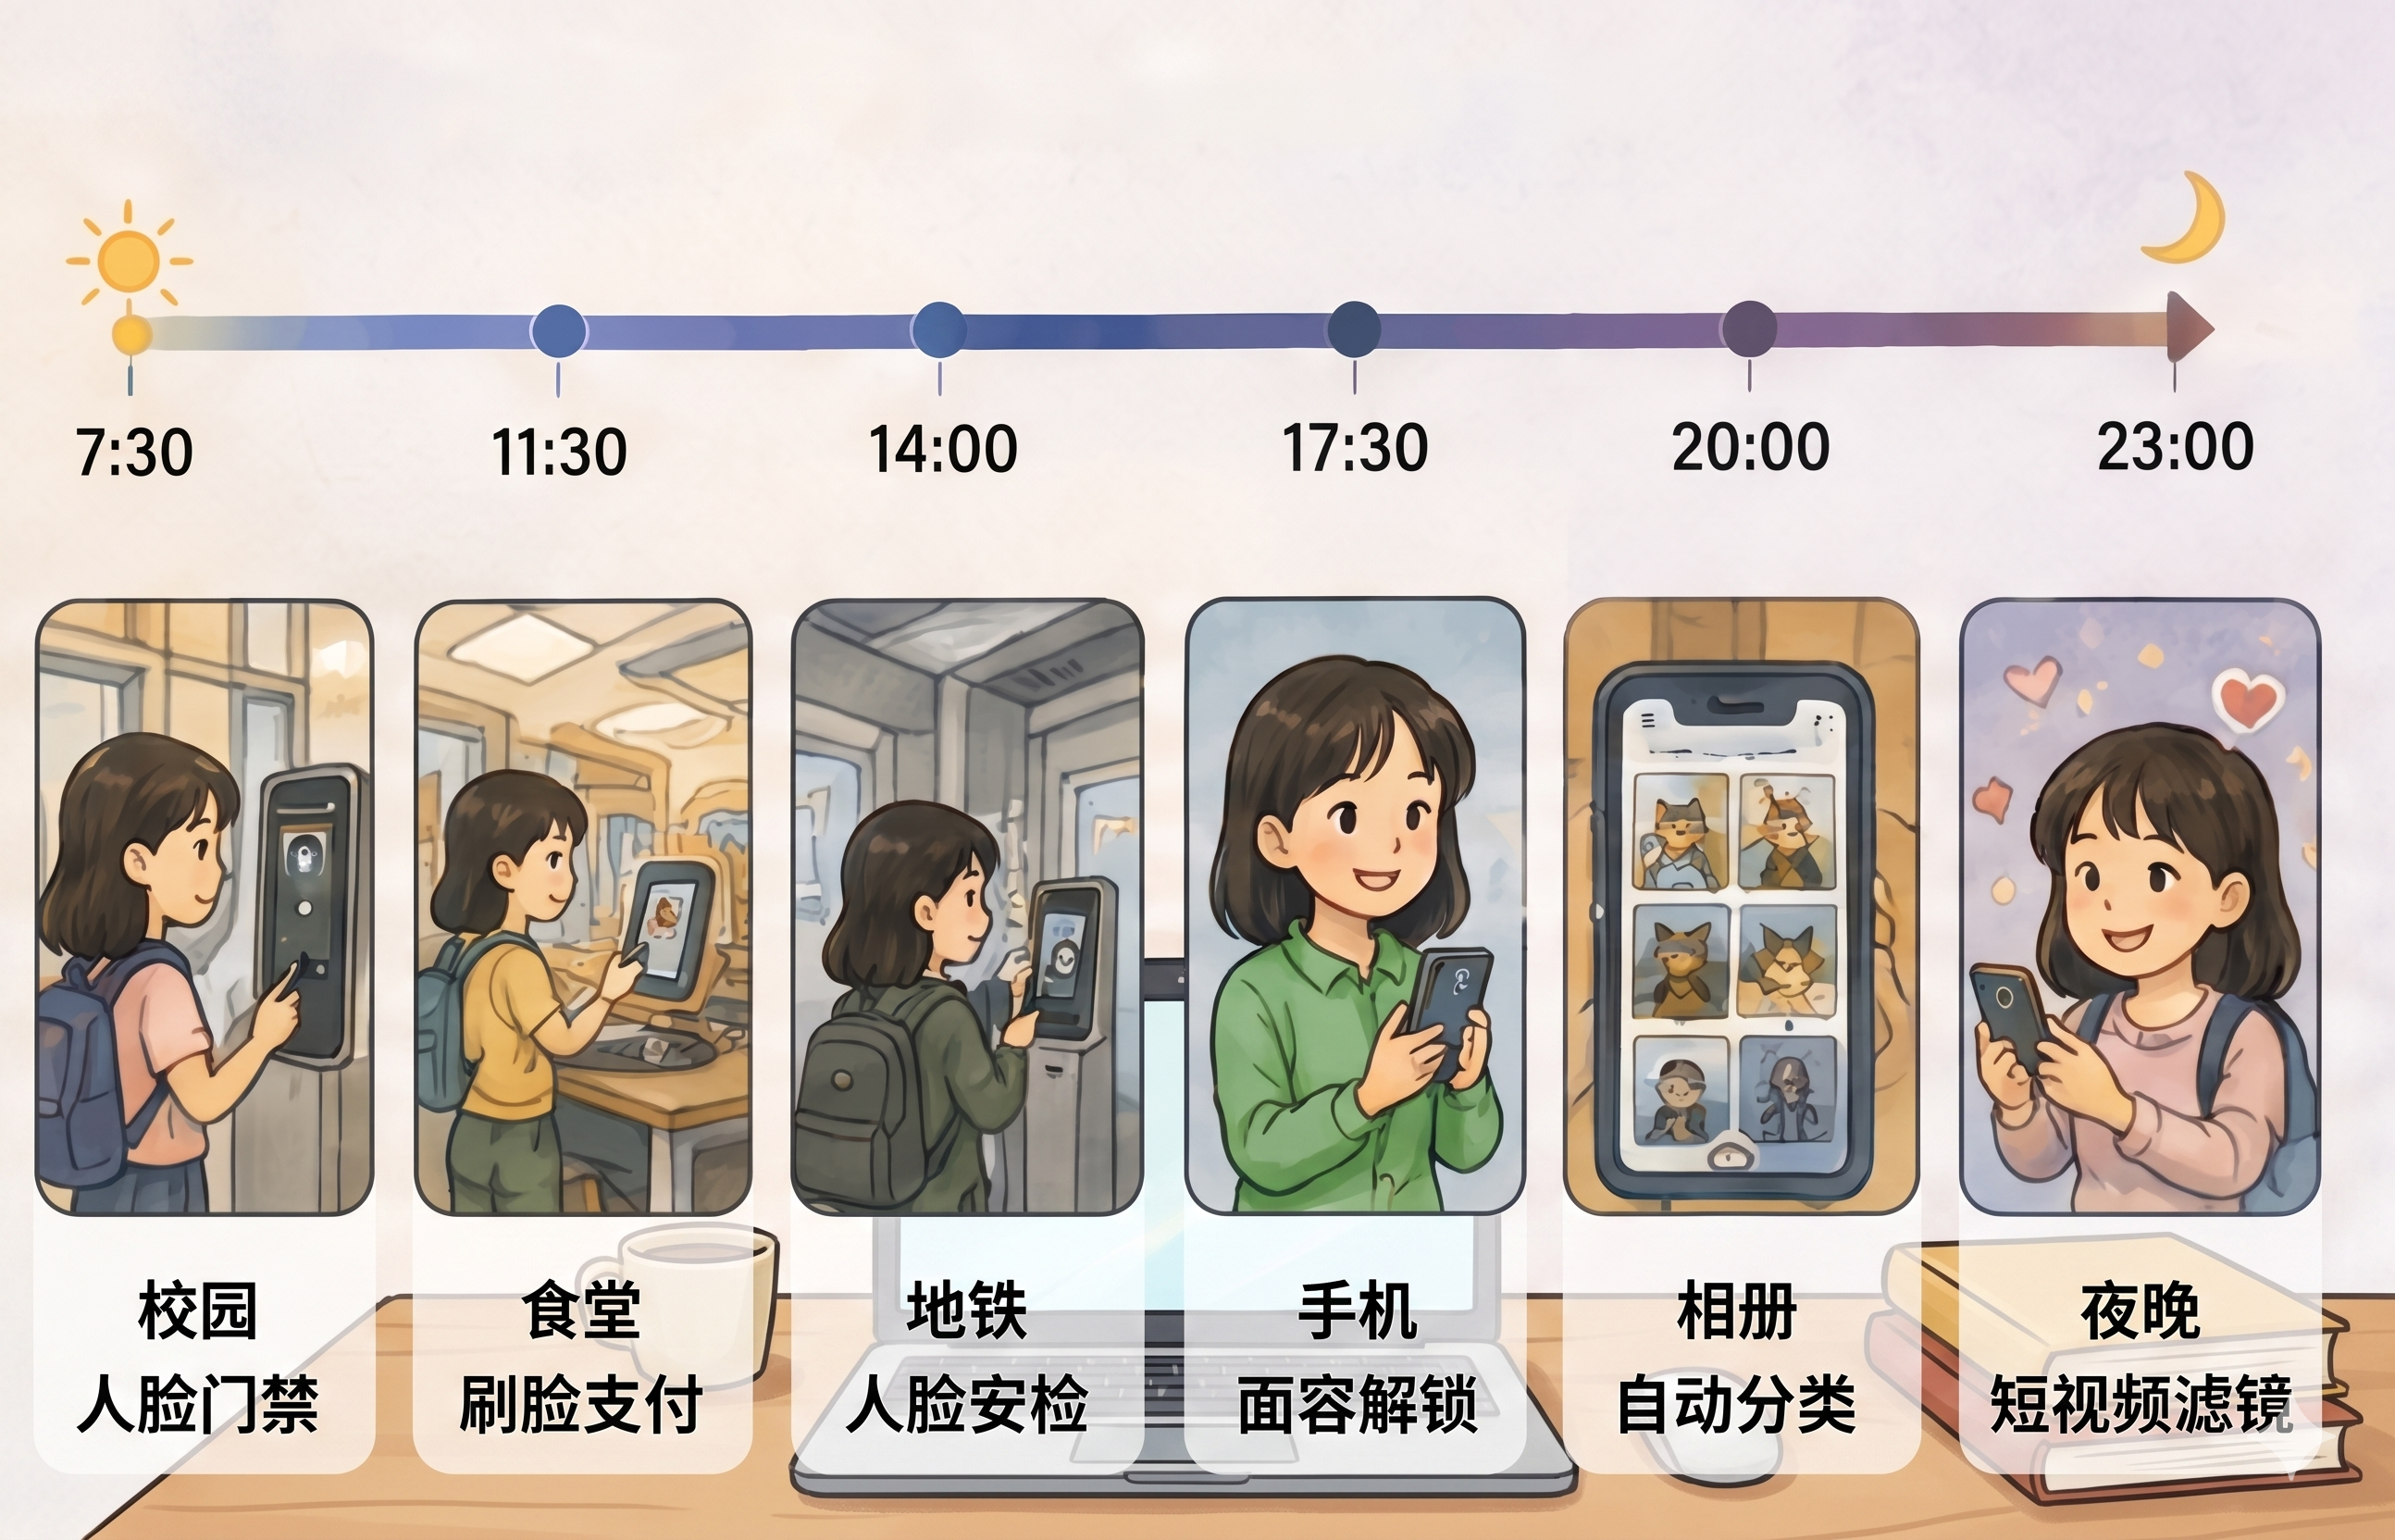
\includegraphics[width=0.88\textwidth]{images_chapter_01-03/2-6.png}
\caption*{\footnotesize\itshape\color{gray!50} 图2-2\quad 推荐系统如何从行为数据中“拼出”用户画像}
\end{figure}

所以，\textbf{AI的“看见”，本质上是一种特征匹配。} 它不是“看到”了你的脸，而是提取了你面部的一组数字特征，然后去数据库里找“有没有哪个已记录的人脸特征和这组数字高度相似”。

那么，AI具体是怎么“提取特征”的？它怎么从一堆像素数字里找出“这是眼睛”“这是鼻子”？

\subsection{计算机视觉——把图片变成AI能理解的“密码”}

让我们做一个简单实验。拿出手机，打开一张照片。用手指放大、再放大、继续放大……直到不能再放大为止。你看到了什么？

一个个纯色的小方格。这就是\textbf{像素}——数字图像的最小单位。一张1920×1080分辨率的照片，由大约200万个像素组成。每个像素有自己的颜色数值（比如R:182, G:207, B:236——这是一种淡蓝色），AI接收到的就是这200万个数字。

从这200万个数字中认出“这是我的朋友在笑”，是计算机视觉要解决的核心问题。AI做到这一点，靠的不是某种神秘的“理解”，而是一个可以被拆解为三个步骤的过程：\textbf{检测→识别→理解场景。}

\begin{figure}[H]
\centering
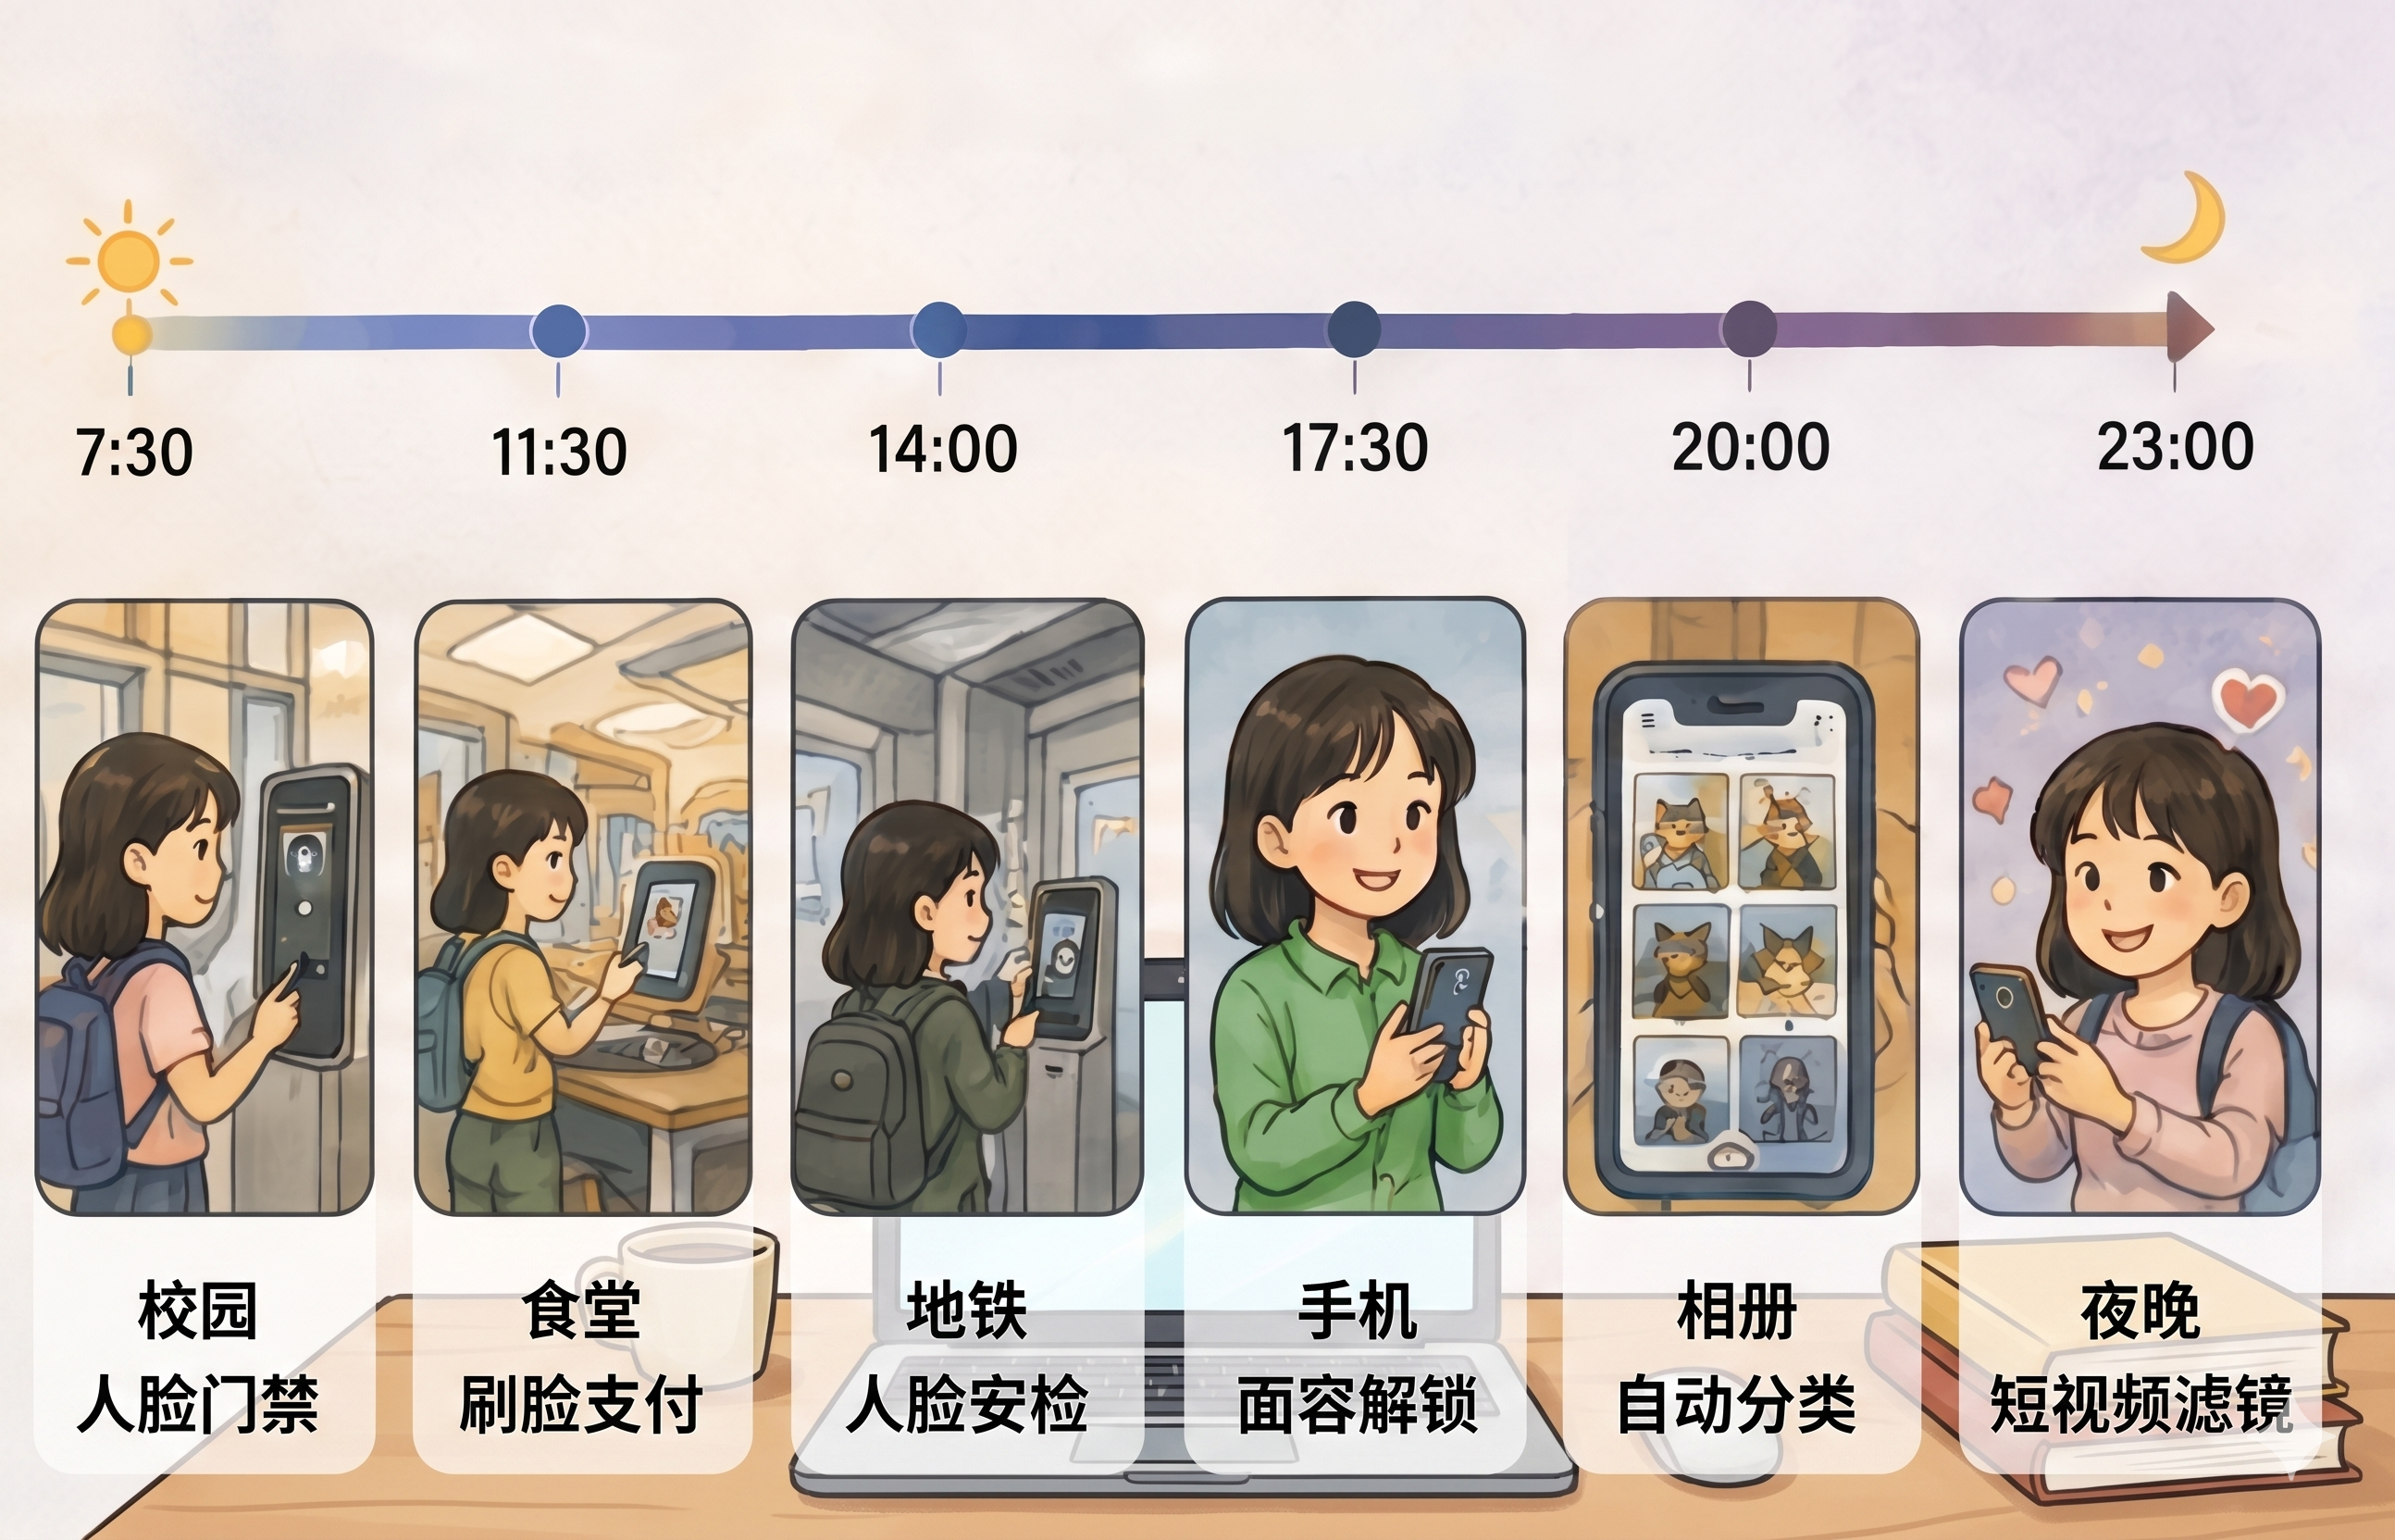
\includegraphics[width=0.88\textwidth]{images_chapter_01-03/2-6.png}
\caption*{\footnotesize\itshape\color{gray!50} 图2-2\quad 推荐系统如何从行为数据中“拼出”用户画像}
\end{figure}

\textbf{第一步：检测——画面中“有什么东西”？} AI会在图像中寻找明暗变化剧烈的区域（那里很可能是物体的边缘），寻找颜色突然过渡的线条（那里可能是物体的轮廓），寻找与周围纹理明显不同的小块（那里可能是一个独立的物体）。当这些局部特征足够多、排列成某种有规律的组合时，AI就会判断：这里可能有一个物体。

\textbf{第二步：识别——这个物体“是什么”？} AI看过数百万张标注了“这是猫”的图片后，内部参数逐渐调整，最终形成了一套对“猫的视觉特征”极其敏感的检测系统。这套系统能从各种角度、各种光照、各种品种的猫身上提取出共同的视觉模式——某种耳朵轮廓的曲率范围、某种眼睛间距与脸宽的比例、某种毛发纹理的统计特征。AI自己也不知道这些模式“意味着”什么，它只知道当这些特征同时出现时，输出“猫”这个标签的概率最高。

\textbf{第三步：场景理解——这些物体之间“是什么关系”？} 这是最难的一步。AI能认出画面中有一个女孩、一个气球、一片草地，但“女孩在公园里高兴地拿着气球”——这个融合了物体关系、场景属性、情绪判断的综合理解，AI目前仍然非常吃力。

\begin{knowledgebox}
\textbf{特征提取——侦探在犯罪现场寻找线索}

AI从像素中提取有用信息的过程，在术语上叫\textbf{特征提取}。你可以把它想象成一位侦探调查犯罪现场：他不需要把整个房间原封不动地搬回警察局，只需要带走关键的指纹、血迹样本、几帧监控录像。AI看图也是同样的逻辑——它不看整张照片，而是提取那些最关键的特征（边缘、形状、颜色分布），然后与数据库中已知物体的“特征档案”做比对。这种“只见树木、不见森林”的做法，正是AI视觉效率极高的原因，也是它时常闹笑话的根源。
\end{knowledgebox}

理解了这三步，你就能回答本节开头的问题了：\textbf{AI不是真正“看见”了世界，它只是在提取视觉特征并进行模式匹配。} 它看到的是数字、是统计规律，而不是物体本身。它不知道“猫”摸起来是什么感觉，“阳光”照在脸上有多温暖，“微笑”背后是什么心情。它只知道当像素排列成某种模式时，输出“猫”的标签；排列成另一种模式时，输出“微笑”的标签。

接下来你可能想知道：既然AI这么擅长模式匹配，它在现实生活中到底能派上什么用场？

\subsection{计算机视觉应用案例}

计算机视觉是当前应用最广泛的AI技术之一。在医疗领域，它帮助医生从CT和X光片中筛查早期病灶；在工业领域，它在生产线上以微米级精度检测产品瑕疵；在农业领域，它通过无人机航拍分析作物长势和病虫害；在体育领域，它追踪运动员的每一个关节动作优化训练方案；在交通领域，它让自动驾驶汽车“看”清路况；在安防领域，它实时分析监控视频识别异常行为；在你的手机里，它自动分类相册照片、解锁屏幕、为短视频添加特效滤镜。

下面，我们通过三个来自不同领域的案例，看看计算机视觉具体是如何运作的。

\subsubsection*{案例1：AI怎样帮助医生发现早期癌症}

2023年秋天，江苏。一位50岁的男性因轻微咳嗽去医院就诊。常规X光胸片显示肺部纹理略增粗，放射科医生判断“无明显异常”，建议按支气管炎处理。

然而，这家医院同时部署了AI辅助影像筛查系统。在医生离开阅片室之后，AI自动重读了同一张X光片。它在右肺上叶区域标注了一个直径约7毫米的微小结节。这个结节的密度只比周围肺组织高出不到10\%，在肉眼直视下几乎无法分辨——就像在灰布上找一块略浅一点的灰斑。AI将其标注为“高风险：建议CT进一步检查”。

正是这个冷冰冰的标注提醒了医生。患者接受了CT扫描，结果确认那是一个早期肺腺癌病灶——直径不到8毫米，尚未扩散，完全可以手术切除。三个月后，手术成功，患者康复。

这个案例里的AI，训练数据来自全国多家三甲医院超过一百万例已标注的肺部CT和X光影像。在训练过程中，它学会了识别那些连资深放射科医生也可能漏掉的细微视觉模式：某些特定的纹理组合、某些特定形态的密度变化、某些特定位置的微小不对称。

但AI也不是完美无缺的。在另一组测试中，同一套系统在22\%的病例中将良性钙化点误判为可疑结节，在约5\%的病例中将早期癌变漏判为正常。这就是为什么它只做“初筛”，最终诊断必须由医生来做。AI不会替代医生，但它让医生多了一双永不疲倦、不会因为阅片到第200张而注意力涣散的“第二双眼睛”。

\subsubsection*{案例2：AI质检员怎样守护你的手机屏幕}

你每天滑动的手机屏幕，在出厂前要经过AI质检的严格把关。

在手机玻璃盖板生产线上，每块盖板只有零点几毫米厚，却要经过数十道工序。任何一道工序中出现划痕、气泡、色差或边缘崩缺，都会影响最终产品的质量。过去，这条质检线靠人眼来完成——质检员坐在强光灯下，一块一块地翻看玻璃盖板，寻找微米级别的瑕疵。一个人一天要看上千块，眼睛疲劳后很容易漏检。而且人跟人之间的判断标准也不完全一致——有人严格，有人宽松。

现在，高速工业相机以微米级精度扫描每一块盖板，AI系统实时分析图像，检测划痕、气泡、色差和边缘缺陷。它不会疲劳，不会因为今天心情不好而误判，检测标准也不会因人而异。在富士康的某些产线上，AI质检系统每天检测超过百万个零件，漏检率远低于传统人工质检。

更有意思的是，AI质检还能做“预防性分析”。如果系统发现某一批次的产品中某个特定位置反复出现同类型瑕疵，它会自动发出预警——这可能意味着生产线上某个环节出了微小的问题，比如注塑模具的某个角落开始磨损。在问题变得严重之前就被发现和修正，避免了大量次品的产生。

\subsubsection*{案例3：AI怎样帮农民“看”庄稼}

在黑龙江的一家大型农场里，搭载多光谱摄像头的无人机正飞过一望无际的麦田。

无人机拍下的不是普通照片，而是多光谱图像——它能捕捉到人眼看不到的近红外光反射。健康的作物叶片会强烈反射近红外光，而缺水、缺肥或遭受病虫害的作物，其光谱反射特征会发生变化。这种变化在肉眼能察觉之前就已经在光谱数据中显现了。

AI系统分析这些光谱数据，判断每一块田地的作物健康状况。哪里缺水、哪里缺氮肥、哪里可能出现了早期病虫害——AI生成一张“农田处方图”，用不同颜色标注不同区域的需求。施肥机按照这张图的指引，在需要的地方精准施入所需量的肥料，而不是整片地均匀撒播。

这套系统让施肥量减少了约15\%，同时产量提升了约8\%。因为在过去，农民只能凭经验整片地施同样多的肥——有些地方施多了浪费，有些地方施少了减产。AI让农业从“看天吃饭”变成了“看数据吃饭”，每一株作物都得到了最适合它的照料。

\begin{knowledgebox}
\textbf{多光谱图像——植物健康的“透视镜”}

普通相机只能记录红、绿、蓝三种颜色，而\textbf{多光谱相机}能看到人眼看不见的近红外光。健康植物在近红外波段会强烈反射——就像给自己拍了一张“健康证明”。一旦植物缺水或患病，反射率就会下降。AI通过分析这些肉眼不可见的光谱变化，可以在症状显现之前就发现问题。这项技术最早用于卫星遥感监测大范围植被，如今随着无人机成本下降，已经飞入了寻常农田。
\end{knowledgebox}

\subsection{AI真的“看懂”图片了吗}

先看一个经典翻车现场。

一位研究者做了一个实验：他找了一张哈士奇站在雪地里的照片，让AI判断照片里是什么动物。AI信心十足地给出答案：“狼。”为什么？因为AI训练数据中狼的照片大多背景是雪地或森林。它没有学会“狼的生物学特征”，它学会的是“雪地背景+黑白毛色≈狼”。

类似的故事还有：一只猫穿上了狗的万圣节服装（衣服上有狗耳朵造型），AI判断为“狗”——因为它提取的关键特征是“狗耳朵形状的轮廓”。一张毕业照，人类看到的是青春、友谊和离别，AI看到的是“一群人穿着相似的衣服站成几排”。

\begin{figure}[H]
\centering
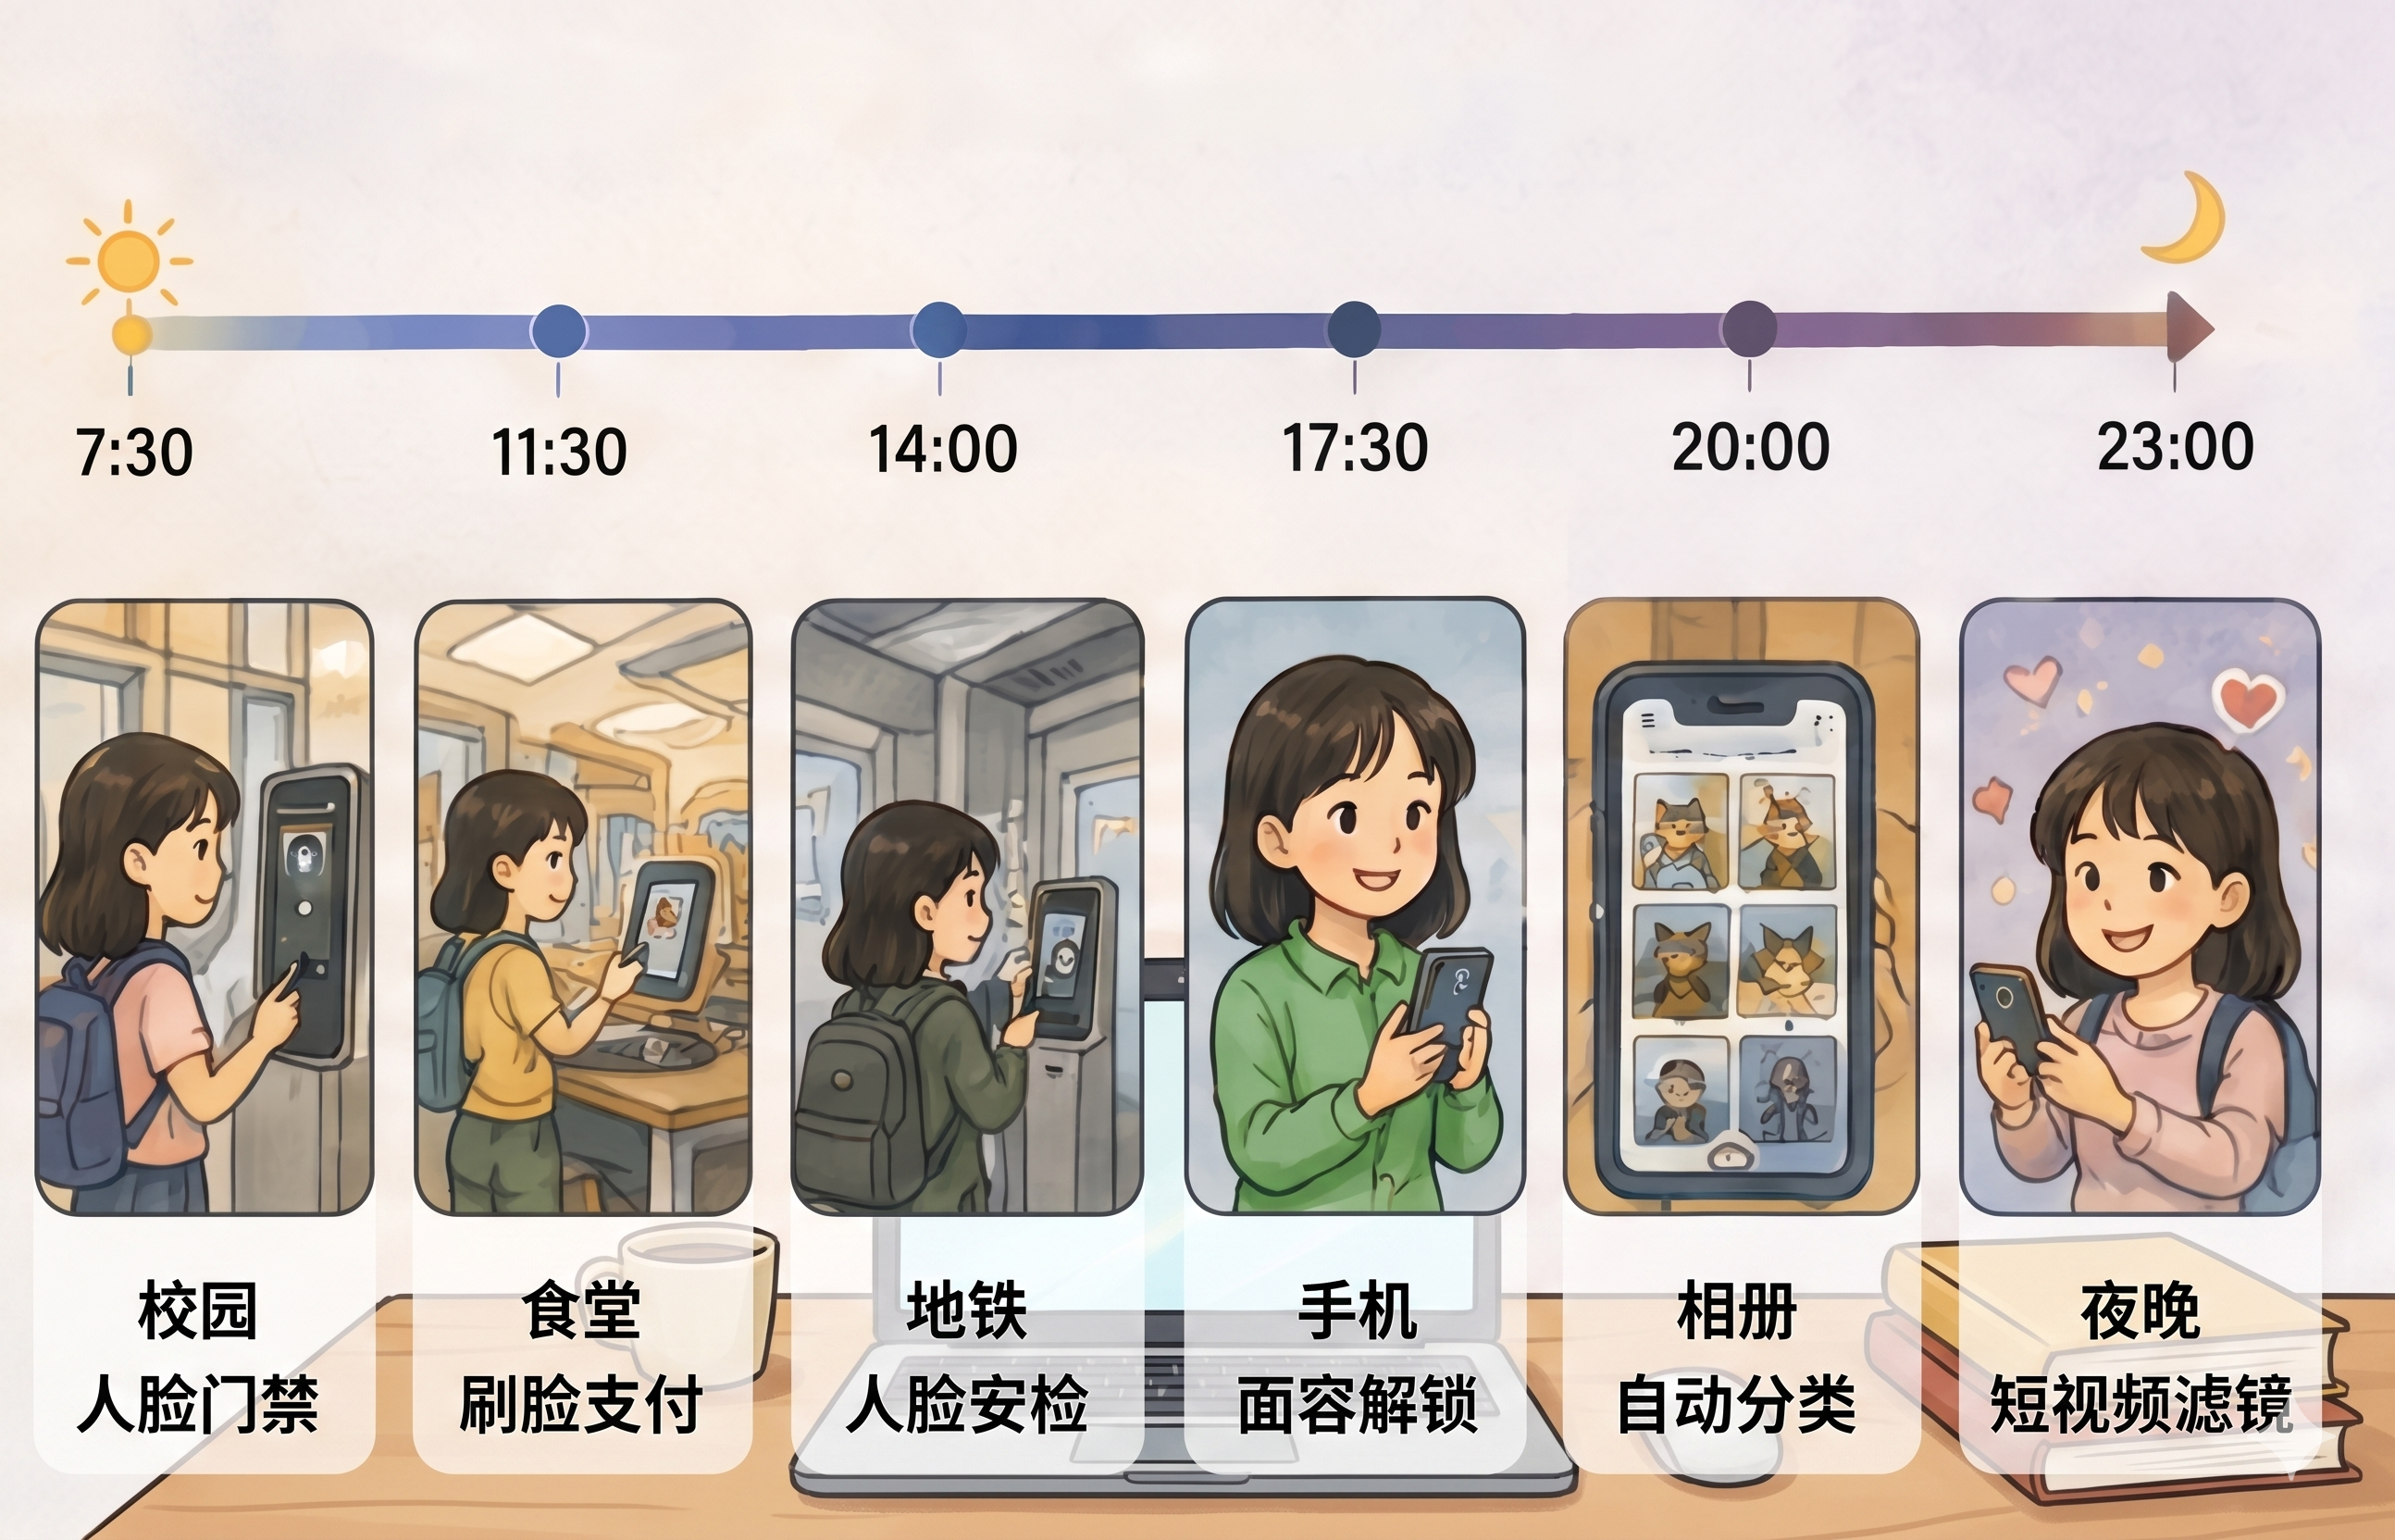
\includegraphics[width=0.88\textwidth]{images_chapter_01-03/2-6.png}
\caption*{\footnotesize\itshape\color{gray!50} 图2-2\quad 推荐系统如何从行为数据中“拼出”用户画像}
\end{figure}

这些翻车案例揭示的，是计算机视觉的三条根本局限：

第一，\textbf{识别不等于理解。} AI能告诉你“这是一张毕业照”，但它不知道毕业意味着什么——它不知道这群人在一起生活了四年，不知道有人在快门按下时忍着眼泪，不知道十年后这张照片会被反复翻出来看。AI看到的只是像素和特征，不是意义和情感。

第二，\textbf{严重依赖训练数据。} AI只“认识”它“见过”的东西。如果训练数据里黑猫的照片太少，AI面对黑猫就可能犹豫或出错。

\begin{funbox}
\textbf{当人脸识别遇上肤色差异——一个MIT实验室的发现}

2018年，麻省理工学院（MIT）媒体实验室的研究生乔伊·布兰维尼（Joy Buolamwini）在做人脸识别实验时，发现了一个让她震惊的问题。当时市面上的主流人脸识别系统在她脸上完全不起作用——她是黑人女性。她尝试了各种方法：调整灯光、改变角度、摘下眼镜——系统始终无法稳定识别她的脸。

百思不得其解的她做了一个实验：在脸上戴上一个白色面具。结果系统立刻成功识别了——识别的是面具，而不是她的脸。

这个发现后来催生了著名的“Gender Shades”研究。研究结果显示，在当时的主流商业人脸识别系统中，浅肤色男性的识别错误率最低（不到1\%），而深肤色女性的错误率最高（可达35\%）。原因不是算法“歧视”——而是训练数据严重失衡。这些系统在训练时使用了大量浅肤色人脸样本和大量男性人脸样本，深肤色女性样本严重不足。AI只是忠实地反映了它“见过”的世界。

布兰维尼的故事后来被广泛报道，并直接推动了多家科技公司改进人脸识别系统的训练数据多样性。它告诉我们：AI的“眼睛”看到的世界，取决于人类给它看了什么样的世界。
\end{funbox}

2018年，MIT的研究者发现，市面上的主流人脸识别系统在识别浅肤色男性时错误率不到1\%，但在识别深肤色女性时错误率可高达35\%——原因不是算法“歧视”，而是训练数据中深肤色女性样本太少。

第三，\textbf{没有常识和推理能力。} AI看到一张“人在水里骑自行车”的图片不会觉得奇怪——因为它不知道水面不能骑车。它没有在现实世界中生活过一天，不知道水是液体、液体会流动、人站在液体上会沉下去。这些对人类来说最基本不过的常识，AI统统没有。

所以，回到本节标题的问题：\textbf{AI真的“看懂”图片了吗？} 答案是没有。它没有“看懂”，它只是在一个极其庞大的视觉特征数据库里，完成了极其高效的模式匹配。“识别不等于理解”——这七个字，是你理解计算机视觉边界的核心钥匙。

接下来，我们要进入一个更让人惊叹的领域——\textbf{自然语言处理}。如果计算机视觉是AI的“眼睛”，那自然语言处理就是AI的“嘴巴和耳朵”。我们将看到AI是如何学会“说话”的，以及——它真的“理解”自己说的话吗？

\section{自然语言处理：AI如何理解和生成语言}

2018年，大三学生小杨去英国交换。出发前，他自信满满地在手机里下载了一款翻译App。落地伦敦后第一次去超市，他想买洗发水，但分不清货架上哪瓶是洗发水、哪瓶是护发素——全是英文。他掏出手机，对着瓶身上的说明拍了张照。翻译结果：“头发营养供应者。使用后，您的头发将拥有丰富的早餐体验。”

丰富的早餐体验？小杨愣了五秒。“我只是想知道这是洗发水还是护发素啊！”

那个年代，社交媒体上流行一个词来形容AI的语言能力：\textbf{人工智障}。早期机器翻译经常闹笑话，智能客服只会回复预设话术，语音助手连“播放周杰伦的歌”都经常听成“播放周结论的歌”。

然后，事情突然变了。2022年11月30日，ChatGPT发布。两个月内，用户突破一亿——成为人类历史上增长速度最快的消费级应用。社交媒体上迅速涌入大量惊叹：有人让它写论文提纲，有人让它讲解高数题，有人凌晨三点和它聊失恋，得到了比一些真人朋友还温柔的回应。

AI突然变得“能说会道”了。它是怎么做到的？

\subsection{AI突然变得“能说会道”了}

让我们从“过去”说起。

早期机器翻译的典型翻车现场可以写成一本书。一句中文“好好学习，天天向上”曾被翻译成“good good study, day day up”——每个单词都对，但拼起来完全不像人话。早期智能客服更是令人崩溃。你问“这门课还有名额吗”，对面永远回复“您好，请先选择您要查询的学期”。早期语音助手也只能完成“打开音乐”“设闹钟”这类简单指令——稍微复杂一点就“我不太明白你在说什么”。

这就是几年前人机语言交互的普遍水平。AI能完成一些简单的语言任务——关键词搜索、固定模板回复、基础翻译——但只要超出预设范围，立刻“智力归零”。

\textbf{然后，2022年底，一切都变了。}

\begin{figure}[H]
\centering
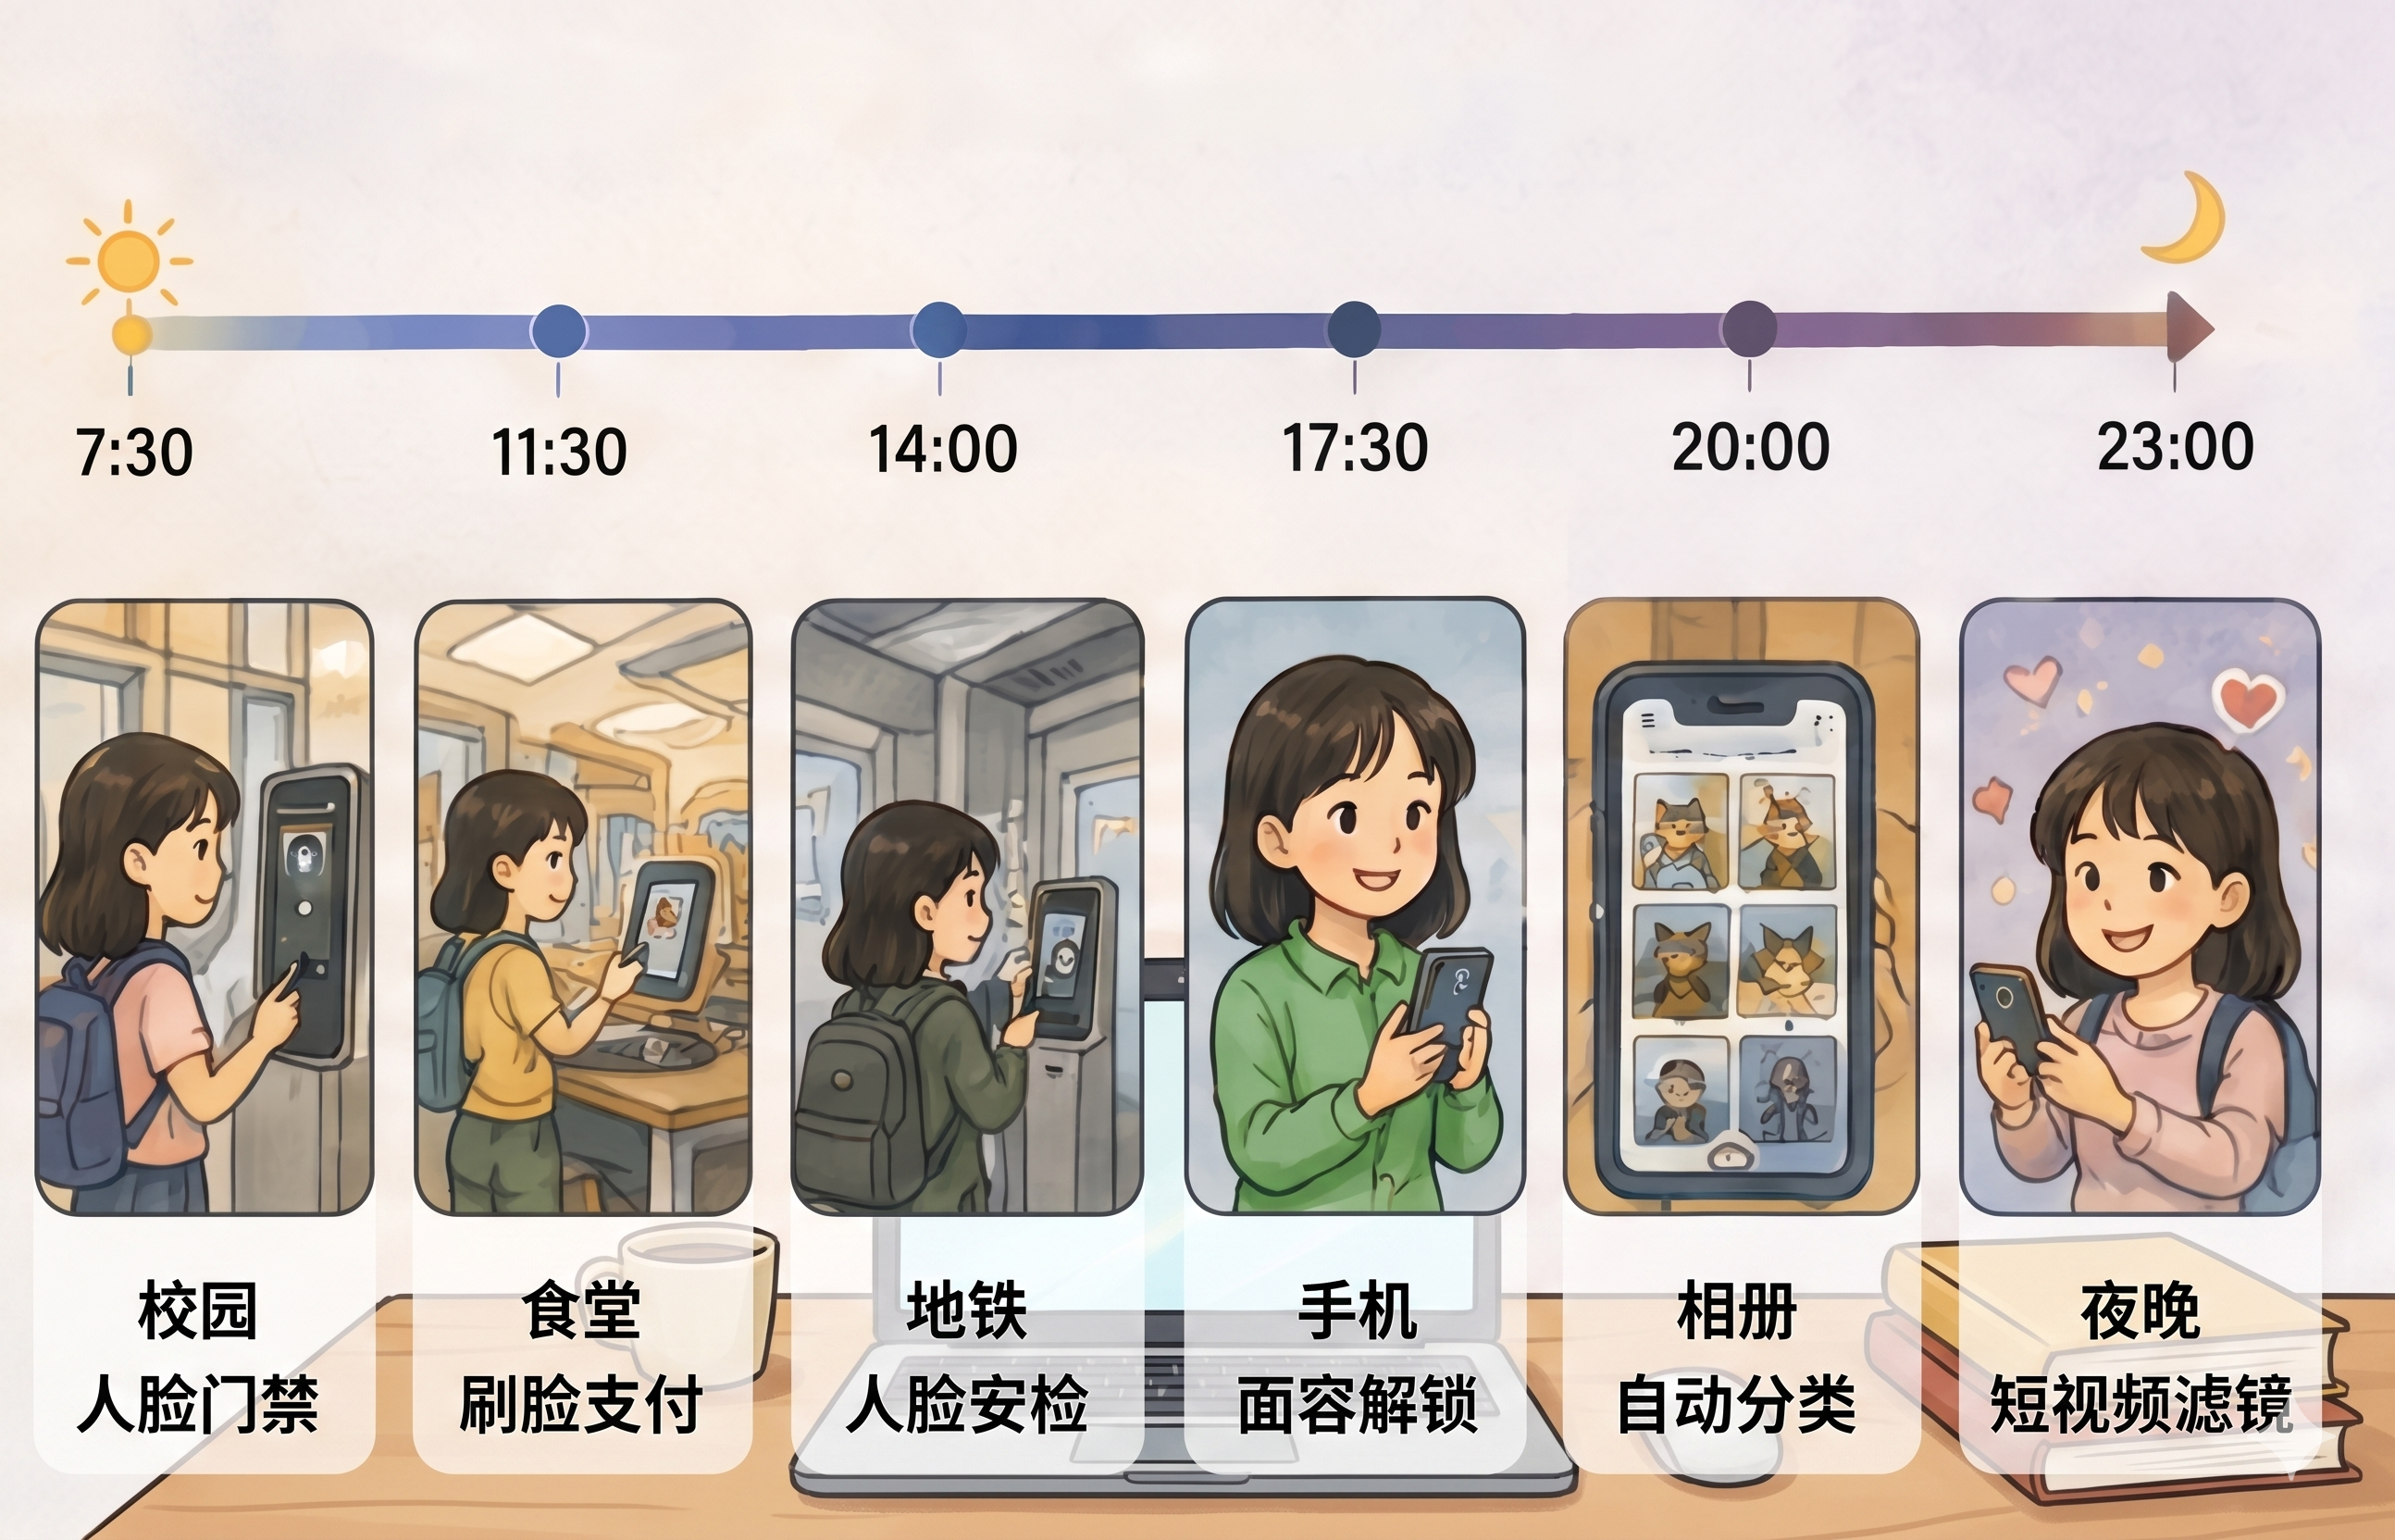
\includegraphics[width=0.88\textwidth]{images_chapter_01-03/2-6.png}
\caption*{\footnotesize\itshape\color{gray!50} 图2-2\quad 推荐系统如何从行为数据中“拼出”用户画像}
\end{figure}

ChatGPT发布后两个月用户破亿。它的出现让大多数人第一次亲身体验到AI“像人一样对话”是什么感觉。紧随其后，DeepSeek、豆包、Kimi等国产大模型迅速进入校园和办公场景。学生用AI整理课堂笔记、总结论文核心观点、生成演讲稿、润色简历。职场人用AI自动生成会议纪要、整理周报。

一位大四学生分享了他的体验：“我上传了一篇十几页的英文论文，跟AI说‘帮我总结核心观点，顺便整理一下考试可能考的重点’。几十秒后，它不仅总结好了，还生成了一个思维导图。以前可能要花两三个小时的事，现在几分钟搞定。”

过去，AI大多只能完成“单一任务”——翻译软件只管翻译，搜索引擎只管搜索，客服机器人只能回复预设话术。而今天的大模型，同一个AI既能聊天、翻译、总结文章，又能写代码、生成PPT、辅导学习。它开始具备\textbf{连续对话、理解上下文、模仿语气和跨任务协作}的能力。

那么问题来了：\textbf{语言明明如此复杂，AI为什么突然能和人顺畅交流了？它真的“听懂”我们了吗？}

\subsection{语言如此复杂，AI为何能“对答如流”}

在回答这个问题之前，让我们先承认一件事：\textbf{理解语言，是人类最了不起的能力之一，也是AI最难以攻克的难题之一。}

想想看，你每天都在接触多复杂的语言现象：同一句话在不同场景下含义完全不同——“你可真行”，有时是佩服，有时是讽刺。网络热词更新比你追的剧还快——从“绝绝子”到“yyds”到“显眼包”。很多人说话根本不按语法来——“你看那个，就是那个，懂我意思吧？”人类瞬间能懂，但机器如果逐字分析，只能一脸茫然。

但AI用一种“绕开理解”的方式，解决了这个难题。它不是像人类那样先理解再表达，而是用统计方法直接“猜”——猜在给定上下文中，下一个词最可能是什么。

\textbf{AI是怎么做到的？答案是：沉浸式学习。}

还记得2.1节我们怎么讲“机器学习”的吗？AI不是靠人工编写规则，而是通过大量例子自己找规律。自然语言处理也是一样。一个孩子学会说中文，不是靠背诵语法书，而是在语言环境中日复一日地听、模仿、被纠正。AI学习语言也是类似过程：它会“阅读”海量互联网文本——新闻、小说、论文、网页、百科、聊天记录、代码、影评……在阅读过程中，它逐渐学会了哪些词语经常一起出现，哪些表达对应哪些语气，什么样的句子结构更符合人类说话习惯。

一个直观类比：想象一个留学生在中国住了二十年。他没上过一节正经中文课，不学语法，不背单词。但他的室友是中国人，他天天一起吃饭聊天；他看中国新闻，刷中国社交媒体，逛中国菜市场。二十年后，他能用中文开玩笑，能听懂“阴阳怪气”，甚至会说方言。AI的语言学习，就是这种“沉浸式学习”的超级加强版——它不是在现实中生活了二十年，而是在几十亿页的文本中“生活”了几个月。

所以，\textbf{AI所谓“听懂语言”，本质并不是拥有真正的人类理解能力，而是通过在海量语言数据中学习规律，对“下一句最可能说什么”做极其精准的概率预测。} 它像一个语言界的“超级模仿者”——模仿得太像了，以至于我们产生了“它真的懂了”的错觉。

那么，AI具体是怎么学习语言规律的？为什么大模型让AI的语言能力突然变得这么强？

\begin{funbox}
\textbf{“心不在焉，不见泰山”——一个经典翻译翻车故事}

在机器翻译的发展史上，有一个广为流传的经典翻车案例。研究者想测试早期的机器翻译系统，输入了一句英文谚语：

“Out of sight, out of mind.”

这句话的本意是“眼不见，心不烦”——见不到的东西就不会惦记。早期的机器翻译系统逐词翻译后给出了英文到俄文的翻译，然后再从俄文翻译回英文。结果变成了：

“Invisible and insane.”

“隐形且疯狂。”

这个结果离原意十万八千里。研究者们捧腹大笑，但这个案例背后揭示的是一个深刻的难题：语言不是单词的简单拼合。同一个短语在不同语境下可能有完全不同的含义，而早期AI完全不具备“理解语境”的能力。今天的AI在这个问题上已经有了巨大的进步——但它是怎么做到的？答案就在下一节要讲的大语言模型中。
\end{funbox}

\subsection{大语言模型——AI的“超级语言大脑”}

要理解大模型，先理解它“大”在哪里。

\textbf{什么是自然语言处理（NLP）？} 简单说，就是“让计算机处理和理解人类语言”的技术。它涵盖了所有和语言相关的AI能力：文字识别、语音转文字、机器翻译、语义分析、对话系统、文本生成。

在ChatGPT出现之前，NLP系统通常只能完成某一个固定任务。翻译软件只会翻译，不会聊天；搜索引擎只会搜网页，不会总结。这个阶段的AI，像只会做一道菜的厨师——你点他拿手的青椒肉丝，他做得又快又好；但你要番茄炒蛋，他只能说“抱歉，我的菜单上没有这道菜”。

\textbf{大模型的出现改变了这一切。}

“大语言模型”（Large Language Model, LLM）中的“大”是关键。过去的AI模型，参数量可能只有几百万到几千万。而ChatGPT背后的GPT-3模型，参数达到了1750亿。后来的GPT-4据说有数万亿参数。参数越多，模型就能学习越复杂的语言规律——就像一个只读过课本的学生，和读过整个图书馆的学生，对世界的理解深度当然不同。

\begin{knowledgebox}
\textbf{参数——AI的“记忆单元”}

\textbf{参数}可以理解为AI模型内部的“记忆单元”或“知识存储位”。每个参数存储着模型从训练数据中学到的一点点信息。当参数只有几百个时，AI只能记住最简单的模式（比如“红色圆形”和“蓝色方形”的区别）。当参数达到1750亿时，AI就能记住极其复杂的语言模式——比如“在悲伤的语境下，应该用什么样的语气和措辞”。GPT-3的1750亿个参数，如果每个参数写在一张便签纸上，这些便签纸摞起来比珠穆朗玛峰还高。换句话说，你每天跟AI聊天，其实是在跟一座“便签纸山”对话。
\end{knowledgebox}

大语言模型学习了几乎所有公开网页文本、大量书籍和文学作品、程序代码、多语言内容。结果是什么呢？同一个AI，既能帮大学生总结论文、帮程序员写代码、帮文案写广告语、帮厨师推荐菜谱搭配、帮老师出考试题。这种从“单一技能”到“通用能力”的跨越，就是大模型带来的核心变化。

\textbf{那么大模型到底是怎么工作的？} 用一句话概括：它本质上是在做“预测下一个最可能出现的词”。当你输入“今天天气很好，我想去\_\_”，它根据学过的语言规律，推断后面最可能接什么词——“公园”“散步”“旅行”“打球”……它选择一个最合理的输出。然后它再根据“今天天气很好，我想去公园”，预测再下一个词。这个过程听起来简单，但当模型足够大、训练数据足够多时，它就展现出了令人惊叹的语言能力。

\begin{figure}[H]
\centering
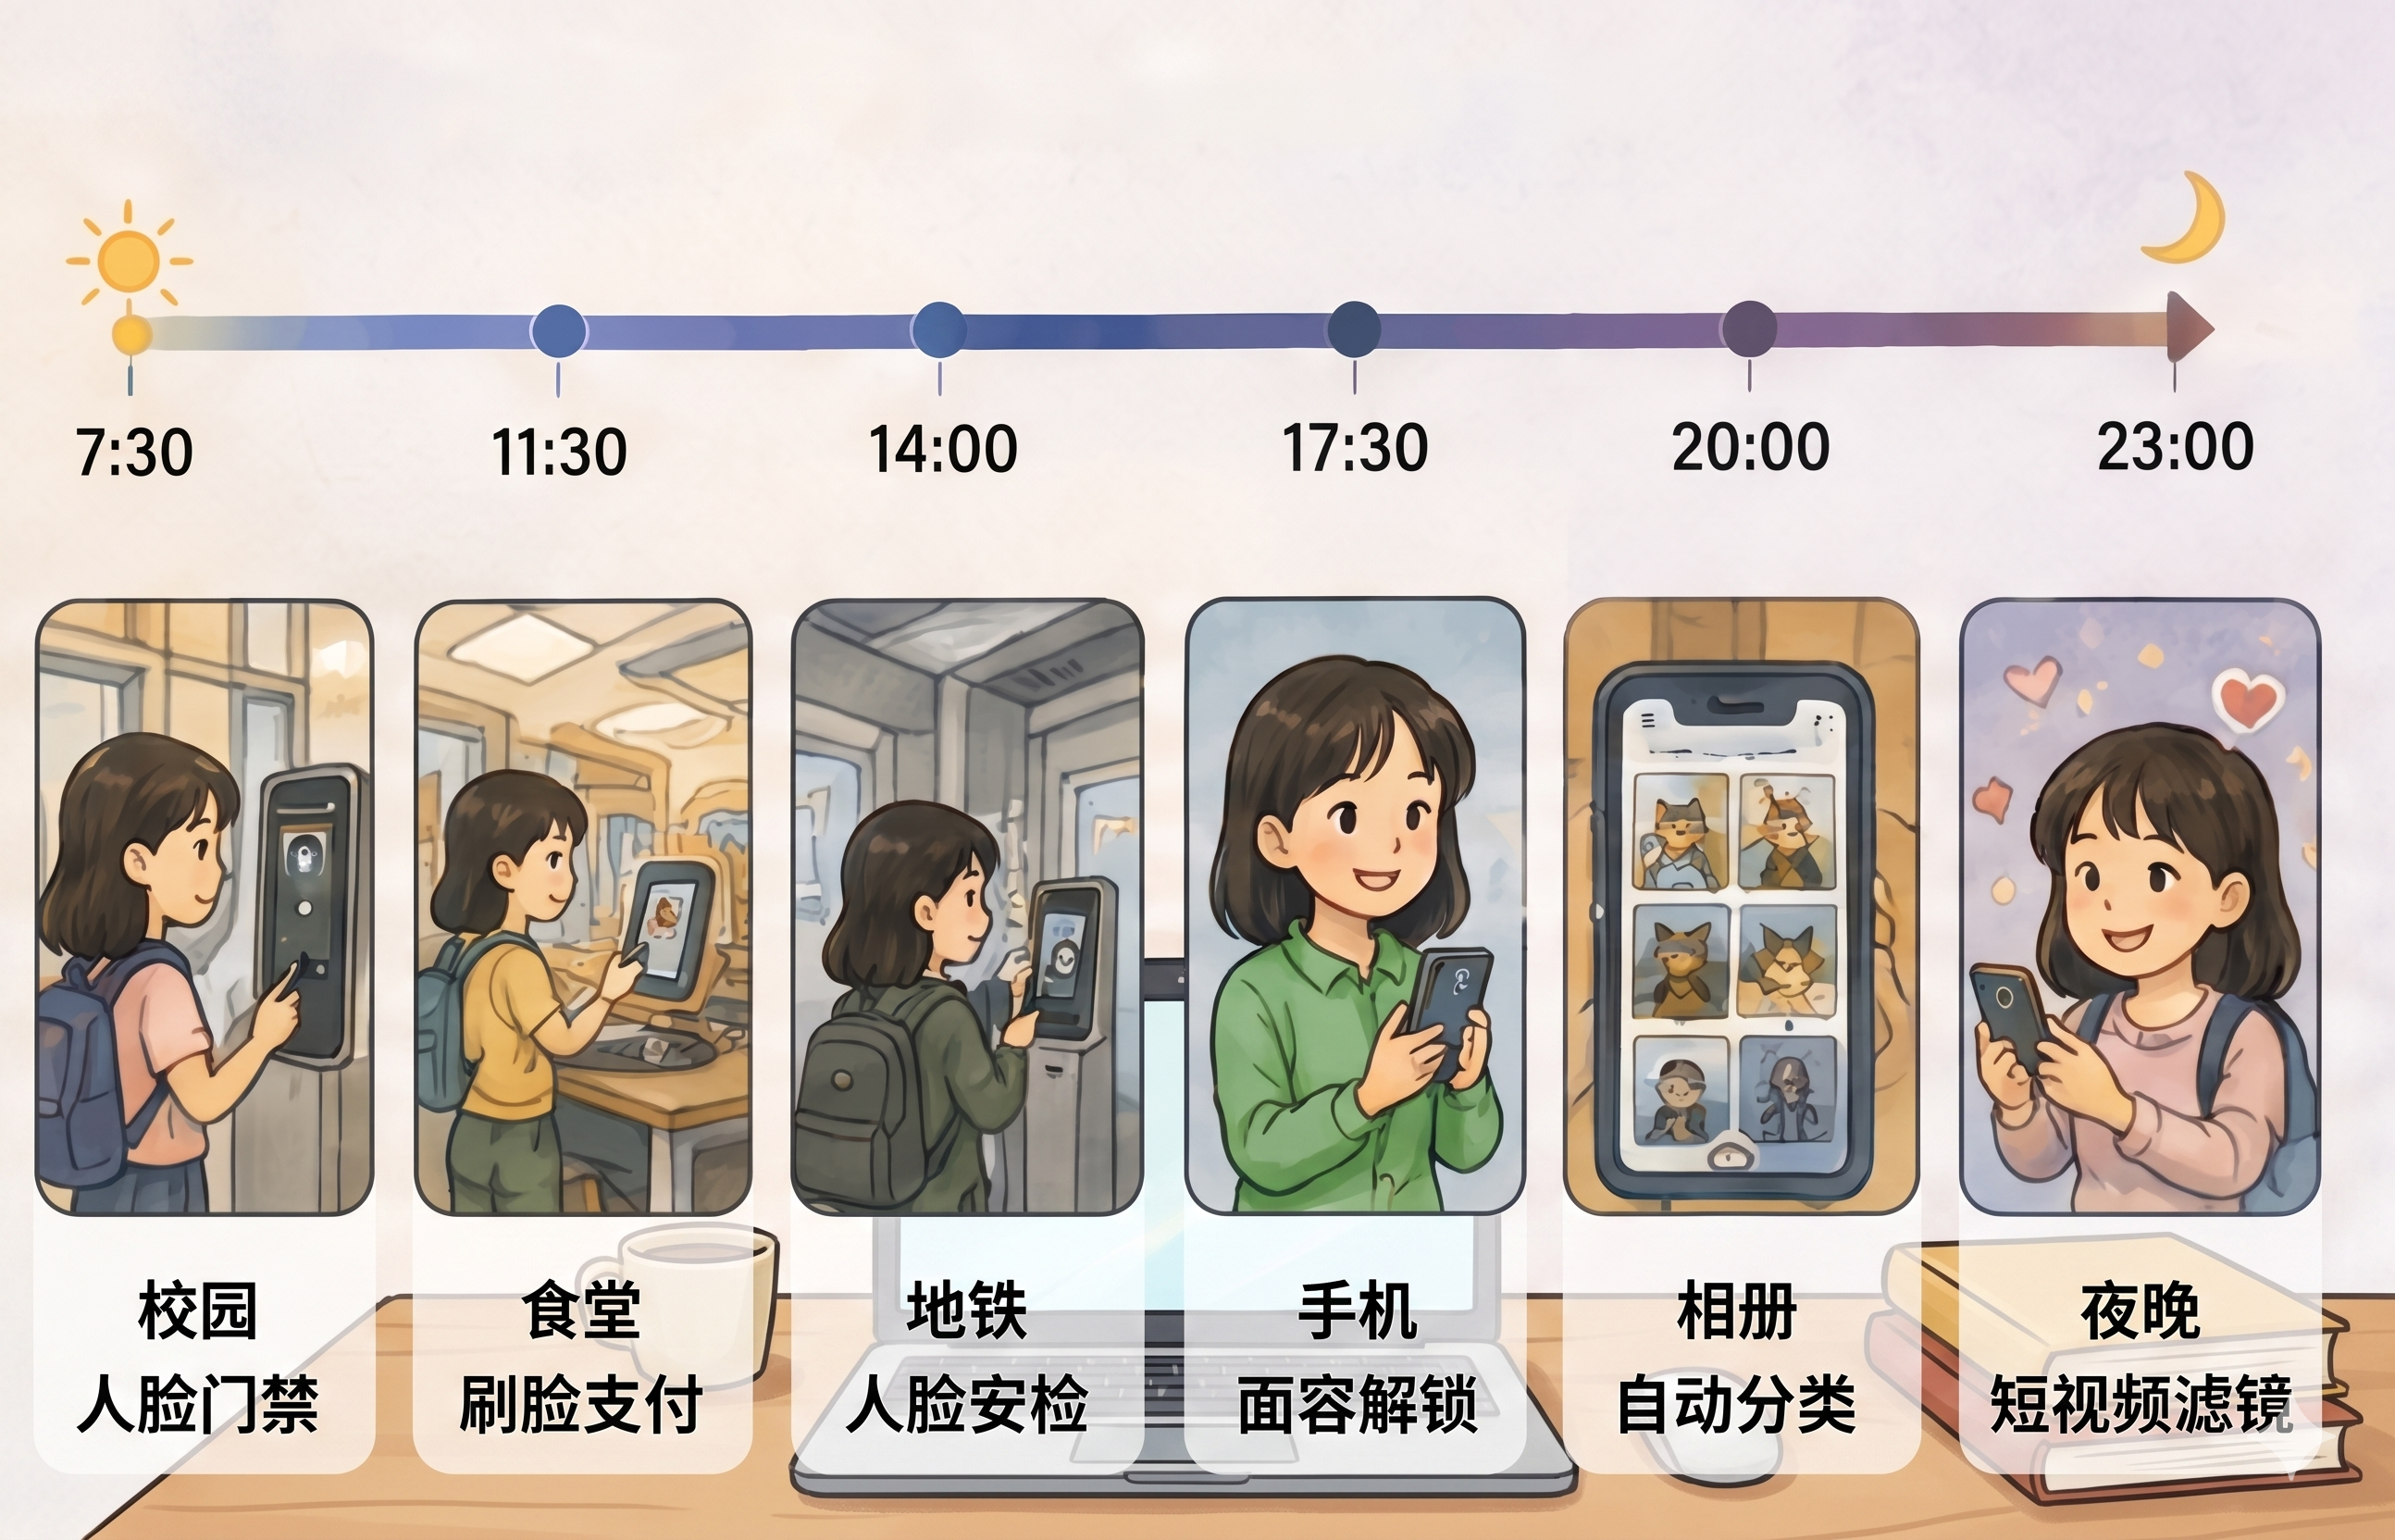
\includegraphics[width=0.88\textwidth]{images_chapter_01-03/2-6.png}
\caption*{\footnotesize\itshape\color{gray!50} 图2-2\quad 推荐系统如何从行为数据中“拼出”用户画像}
\end{figure}

了解了这些原理，我们来看看语言智能在现实生活中到底能做什么。

\subsection{语言智能应用案例}

语言智能正在从“单一任务的工具”变成“跨场景的通用助手”。在学习领域，它帮学生总结论文、整理笔记、辅导语言学习；在办公领域，它自动生成会议纪要、起草邮件、整理周报；在科研领域，它辅助文献检索、翻译外文论文、归纳研究趋势；在医疗领域，它帮医生语音录入病历、整理诊断报告；在娱乐领域，它写剧本、生成歌词、设计对话角色；在跨语言交流中，它让实时翻译从生硬逐字走向自然流畅。

下面，我们通过三个来自不同领域的案例，看看语言智能具体是如何运作的。

\subsubsection*{案例1：AI辅助阅读论文——从三小时到四十分钟}

研一新生小赵正坐在图书馆里，对着电脑屏幕上的一篇英文论文发愁。这是导师让他读的第一篇文献，发表在Nature上，关于蛋白质结构预测的最新研究。十几页正文加上几十条参考文献，光是摘要就有400多个单词，里面好几个专业术语他见都没见过。

过去，一个研究生面对这种情况的标准流程是：逐段翻译——遇到不认识的词查词典；看到专业术语去搜索含义；手动摘录重要段落到笔记本上；最后自己归纳核心观点、研究方法和主要发现。小赵的室友去年就是这么做的。“第一篇论文花了我三个下午，”室友说，“后来熟练了，一篇也要两三个小时。”

但现在，小赵把论文PDF上传到AI工具，输入了一句话：“请帮我总结这篇论文的核心观点，用表格呈现研究方法、主要发现和研究局限性。另外，用通俗的语言解释一下那些专业术语。”

大约二十多秒后，AI给出了回复。它先列了一张简洁的表格：研究方法是什么、主要发现是什么、局限性在哪里。接着，它把论文中像“homologous sequence alignment”“residue co-evolution”这样的专业术语用大白话解释了一遍——不是像词典那样冰冷地给出定义，而是结合论文上下文，告诉你“这个词在这篇论文里的意思是……”。

小赵后来回忆：“我当时的感觉就像——以前是你一个人在黑暗的隧道里摸索，现在突然有人递给你一个手电筒，还说‘这边我走过，跟着我’。”他当然没有把AI的输出照单全收。读完全文后他核对了AI的总结，发现基本准确，只有一个细节有些偏差。他用AI整理的知识框架作为骨架，自己填充了更多阅读后的理解和批判性思考。原本可能花三个小时的工作，变成了大约四十分钟——还包括了与AI来回讨论、追问细节的时间。

这个案例的核心启示是：大模型最大的变化不是“比搜索引擎搜得更准”，而是它从一个“只能做一件事的工具”变成了一个“能辅助整个工作流的助手”。AI不是替代研究者，而是让研究者把精力从繁琐的信息整理中解放出来，投入到更高层次的批判性思考中去。

\subsubsection*{案例2：AI翻译从“生硬逐字”走向“理解上下文”}

如果你用过十年前的翻译软件，应该还记得那种生硬感——每个单词都翻译了，但拼在一起完全不像人话。英文谚语“It's raining cats and dogs”曾有过“正在下雨猫和狗”的著名翻译，让读者一脸茫然。

今天的大模型翻译已经开始结合上下文做更自然的转换。当它读到“It's raining cats and dogs”时，它不只是查词典——它从海量中英文对照文本中学到了，这句话在中文里对应的习惯表达是“下着倾盆大雨”或“雨下得很大”。当它翻译一封商务邮件时，它会根据邮件的正式程度调整语气——不会把“Best regards”翻译成“最好的问候”，而是自然地翻译为“此致敬礼”或“祝好”。

更关键的是，大模型翻译能“理解”整个段落的意思，而不是一句一句孤立地翻。在一篇关于气候变化的英文报道中，同一个词“bank”可能在不同位置分别表示“银行”“河岸”“倾斜”。传统翻译软件可能翻错其中一两处，而大模型通过分析整段话的语境，能正确区分每个“bank”的含义。

一位留学生分享了他的体验：他用AI翻译工具阅读德文哲学论文。过去他需要借助词典逐句啃，现在他先让AI生成一个流畅的中文版本，然后对照原文精读，重点关注那些复杂的论证段落。翻译变成了辅助理解的工具，而不是替代品。

\begin{figure}[H]
\centering
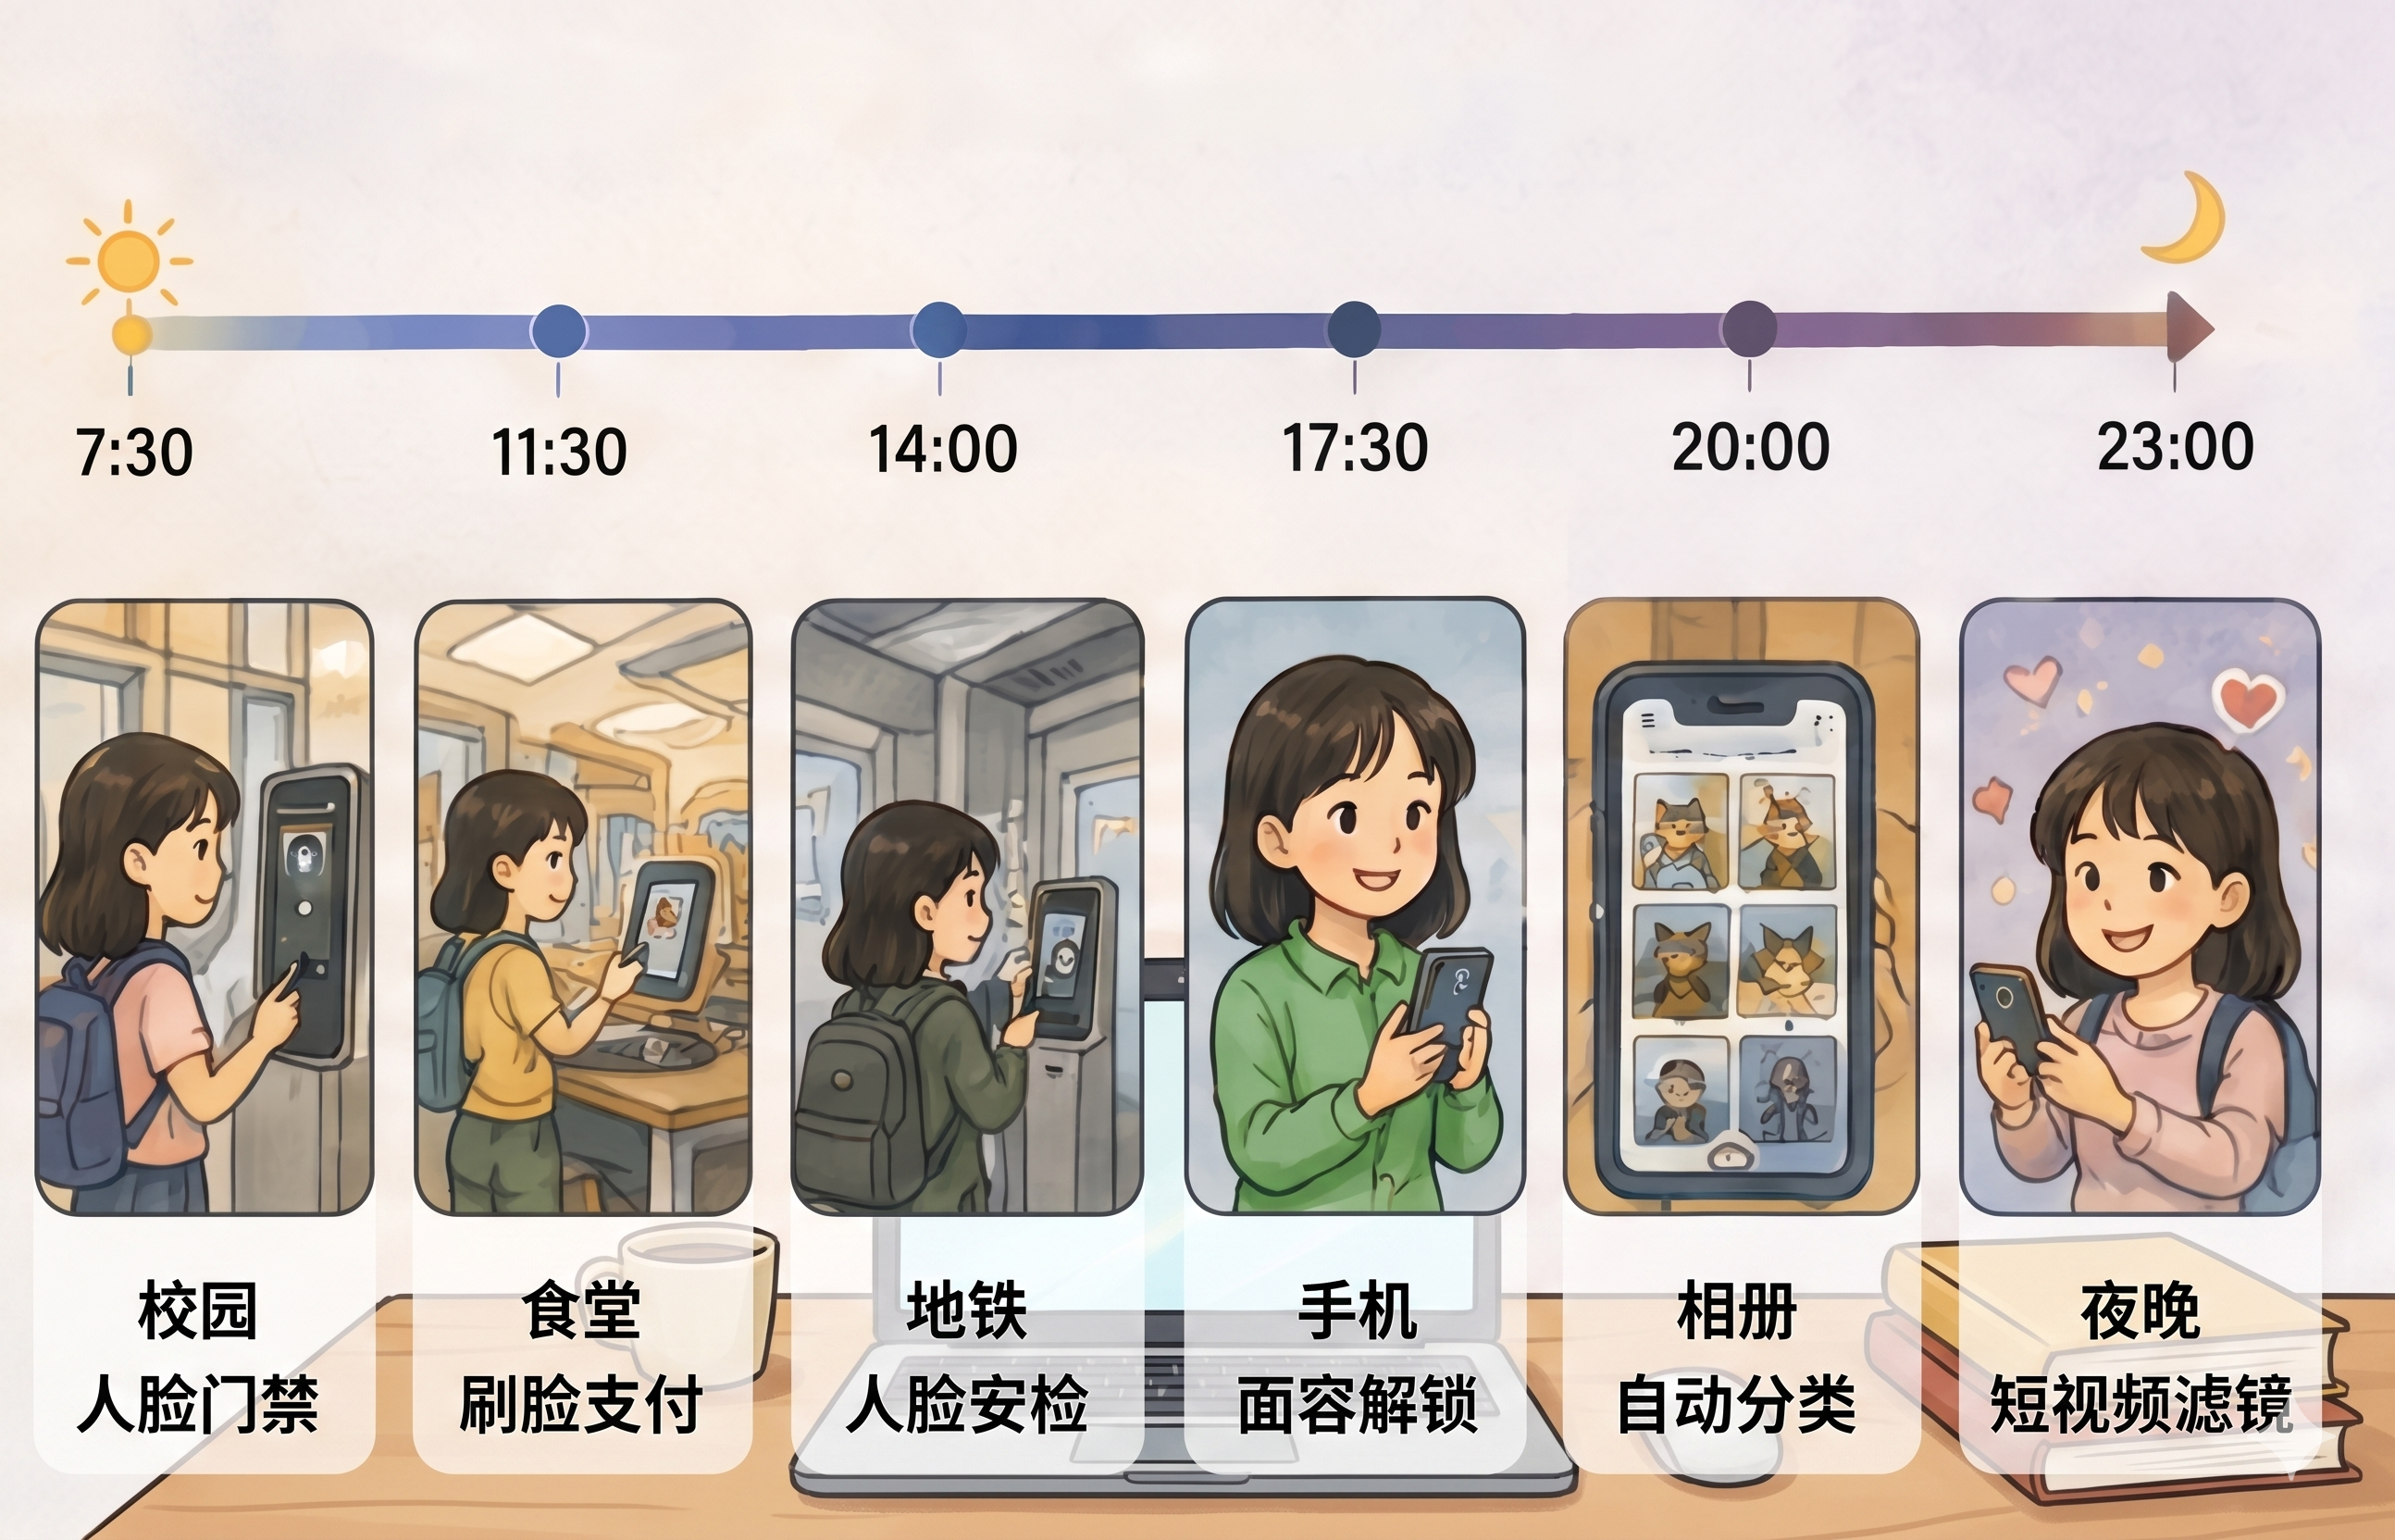
\includegraphics[width=0.88\textwidth]{images_chapter_01-03/2-6.png}
\caption*{\footnotesize\itshape\color{gray!50} 图2-2\quad 推荐系统如何从行为数据中“拼出”用户画像}
\end{figure}

\subsubsection*{案例3：AI语音助手从“执行指令”走向“自然对话”}

“嘿Siri，设一个明早7点的闹钟”——这是传统语音助手能做的事。它能理解关键词“闹钟”和“7点”，然后执行预设的指令。

但如果你说：“帮我查一下明天从北京到上海的高铁，要上午出发、3小时以内的车次，顺便看看上海明天的天气”——传统语音助手可能就糊涂了。这个请求里包含了多个任务（查高铁、筛选条件、查天气），而且任务是嵌套和关联的（先查高铁时间，再根据出发时间看天气）。

现在的大模型语音助手可以处理这样的复杂请求。它先理解整句话的意图——不是简单地识别关键词，而是理解“查高铁+筛选条件+顺便查天气”的完整任务结构。然后它调用火车票查询工具获取车次信息，按照“上午出发、3小时以内”的条件筛选，再调用天气工具查询上海明天的天气。最后把两个结果整合成一段自然的回复：“明天北京到上海上午出发且3小时以内的车次有G1次（9:00-12:28）和G3次（10:30-13:35）。顺便说一下，上海明天多云转阴，气温15-22℃，建议带一件薄外套。”

从“听懂关键词执行命令”到“理解整句话的意图并完成复杂查询”，语音助手正在越来越接近一个真正的“助手”。它不再只是“听懂指令”，而是开始“理解需求”。

\subsection{AI真的“理解”语言吗}

先讲一个真实故事。2023年，美国一位律师在准备一份诉讼材料时，使用了ChatGPT帮他检索相关判例。AI很快给出了六个判例，格式完整——有案件名称、审理法院、判决日期，甚至详细的案件编号。律师把这些内容写进了法律文书，提交给法庭。结果，对方律师在核查时发现：\textbf{这六个判例，一个都不存在。} AI完全编造了它们。

这个故事揭示了一个核心问题：\textbf{AI擅长的是“生成看起来合理的语言”，而不是“陈述事实”。} 用技术术语来说，这叫\textbf{AI幻觉}（Hallucination）——AI在生成内容时，并不知道什么是真、什么是假。它只是在做概率计算：基于你给的提示词，什么词接在后面最合理？如果训练数据中对某个问题没有足够的信息，AI就可能“杜撰”——但它不会告诉你“我不知道”，它会编造一个看起来像真的答案。

\begin{knowledgebox}
\textbf{AI幻觉——一个超级模仿演员的即兴表演}

\textbf{AI幻觉}是指AI生成的内容虽然表达流畅、看起来合理，但包含事实性错误或完全虚构的信息。可以这样理解：AI像一个超级模仿演员，看了无数部法庭电影，学会了律师说话的方式。你让他即兴来一段“律师在法庭上的慷慨陈词”——语气、用词、逻辑都无可挑剔。但他说的每一个案号、每一条法条，都是根据“应该这样演”而编出来的。AI就是这位演员。它没有被设计成“诚实”，而是被设计成“继续接龙”。这解释了为什么它能在法庭上“义正词严”地引用根本不存在的判例。
\end{knowledgebox}

类似的故事还有很多：有人让AI推荐旅游攻略，AI推荐了一个根本不存在的景点；有人让AI解释一道物理题，AI条理清晰地给出了错误答案；有人和AI聊得投机，但发现AI完全理解不了讽刺和隐喻——你说“今天真是个好日子”（其实你在反讽，因为出门就被雨淋了），AI会认真地回复你：“是的，晴天总是让人心情愉快。”

所以，回到本节的核心问题：\textbf{AI真的“理解”语言吗？}

答案很明确：\textbf{不，它不理解。} AI是一个超级模仿者。它读过人类写过的几乎所有东西，学会了人类使用语言的各种模式。它能生成优美、流畅、看似有理有据的回答。但它对自己输出的内容没有“真伪判断”。它不知道自己是在陈述事实还是在编造故事。它可以在几秒钟内写出一篇论文，但不知道那篇论文的质量和真实性。它可以回复你“我理解你的感受”——但它没有感受过任何东西。它不理解悲伤，不理解孤独，不理解爱。

今天的大模型确实让AI的语言能力产生了飞跃。它能辅助学习、办公、创作，效率惊人。但它仍然是工具，不是拥有意识的人类。它输出的一切内容，都需要人类判断是否真实、是否合适、是否可用。真正重要的，不是“AI越来越像人了”，而是我们如何学会正确地使用它，并始终保持独立思考和批判性判断。

\section{生成式AI：机器也能“创造”内容}

2022年8月，美国科罗拉多州。游戏设计师杰森·艾伦（Jason Allen）坐在电脑前，反复修改着输入一段文字描述。他在Midjourney中不断调整提示词，尝试了上百个版本。最终，他选择了一幅作品参赛。这幅画名为《太空歌剧院》（Théâtre d'Opéra Spatial）——一个恢弘的巴洛克式舞台上，身着华丽戏服的演员们沐浴在金色光束中，背景是深邃的星空和巨大的行星。评委将数字艺术类别的最高奖项颁给了它。

然后事情就炸了。媒体蜂拥而至，艺术界分裂为两个阵营。一方说这是作弊——“AI生成的画不应该被称为艺术”。另一方说这是新时代的开端——“就像摄影没有杀死绘画，AI也不会杀死艺术”。杰森·艾伦本人在接受采访时说了一句意味深长的话：“我不是画家，我赢了比赛。我提交的不是一幅画，而是一个声明。”一个什么声明？一个关于“创造力”正在被重新定义的声明。

\subsection{当AI开始画画、写文章、做音乐}

大一学生小陈是校学生会宣传部的干事。新学期开学，他接到一个任务：三天之内设计一张招新海报。他不会用Photoshop，更没学过设计。在过去，他只能求助设计专业的学长或者从网上下载模板来改——结果往往是“改来改去还是像模板”。

但这一次，他打开了一款AI绘图工具。他花了几分钟想清楚自己需要什么，然后输入：“一张现代风格的学生会招新海报。背景是校园标志性建筑的线条简化图，前景是几个抽象的大学生在热烈讨论，配色以校徽的深蓝色为主调、点缀明亮的橙色。画面底部留白，用于放置招新信息和二维码。”

几十秒后，AI生成了四张不同设计风格的海报供他挑选。小陈选了一张最能体现“活力”的，用AI的局部重绘功能把背景中的建筑线条调得更简洁，然后在底部预留的空白处手动加上了招新群二维码。从构思到成品，不到四十分钟。

他把海报发到学生会群里，一位大三的设计专业学姐在群里问：“这次是谁做的？构图挺干净的。”小陈回了一句：“我提的想法，AI执行的。”群里安静了几秒。然后学姐回了一句：“……好吧，看来我也得学学怎么用AI了。”

不只是海报。在宿舍另一边，一位中文系的同学正在用AI润色小说创作的语言。一位计算机系的学生用AI生成了一段原创旋律，准备用在校园微电影的配乐上。过去，这些创作行为各自有着高高的门槛——你要会画画、会写文章、会编曲、会设计。而现在，门槛正在被AI系统性地降低。

你可能会问：\textbf{AI为什么突然“会创作”了？就在几年前，它还只会“认猫认狗”。这个转变是怎么发生的？}

\subsection{AI没有灵感，为什么“创作”的还挺像样}

要回答这个问题，我们得先搞清楚：\textbf{人类是怎么创作的？AI又是怎么“创作”的？}

人类创作一首情歌，可能是因为刚经历了一场刻骨铭心的恋爱。他坐在钢琴前，想起某个人、某个场景、某个瞬间，心里涌出的情感变成了旋律。

AI呢？AI没有恋爱过，没有被分手过，没有在深夜辗转反侧过。但它“听”过数以万计的人类情歌。它分析了无数情歌的旋律走向、和弦进行、歌词节奏——它从中总结出了“情歌通常是这样写的”的规律。当你让它创作一首情歌时，它把那些规律重新组合，生成了一首“听起来像情歌”的歌。

一个很好的类比：一个学生，没去过巴黎，没谈过恋爱，没经历过人生的大起大落。但他临摹过一万张梵高的画。慢慢地，他不仅能画出和梵高原作几乎一模一样的画，还能画梵高没有画过的题材——比如把埃菲尔铁塔画成梵高《星月夜》的风格。他画的不是巴黎，也不是他自己，而是“如果梵高画巴黎，大概会这么画”。

生成式AI就是那个学生。它没有灵感，没有情感，没有生活。但它有几十亿张画作、几亿篇文章、几千万首音乐的训练样本。

\textbf{核心认知}：生成式AI的“创作”，本质不是“表达”，而是\textbf{模仿重组}。它分析海量作品的风格规律，然后根据你的要求，重新组合出一个“看起来像人类作品”的新内容。它不是从无到有地创造，而是在对已有模式进行超大规模的“拼合和变奏”。

\subsection{生成式AI——当AI学会“举一反三”}

先区分两个概念：\textbf{传统判别式AI vs 生成式AI}。

传统AI（也叫判别式AI）的核心能力是“判断”——给它一张照片，它判断这是猫还是狗。给它一封邮件，它判断这是正常邮件还是垃圾邮件。它像一个鉴定师。生成式AI的核心能力是“创造”——给它一行文字描述，它能画出一张全新的画。给它一段提示，它能写出一篇原创文章。它更像一个创作者。

\begin{figure}[H]
\centering
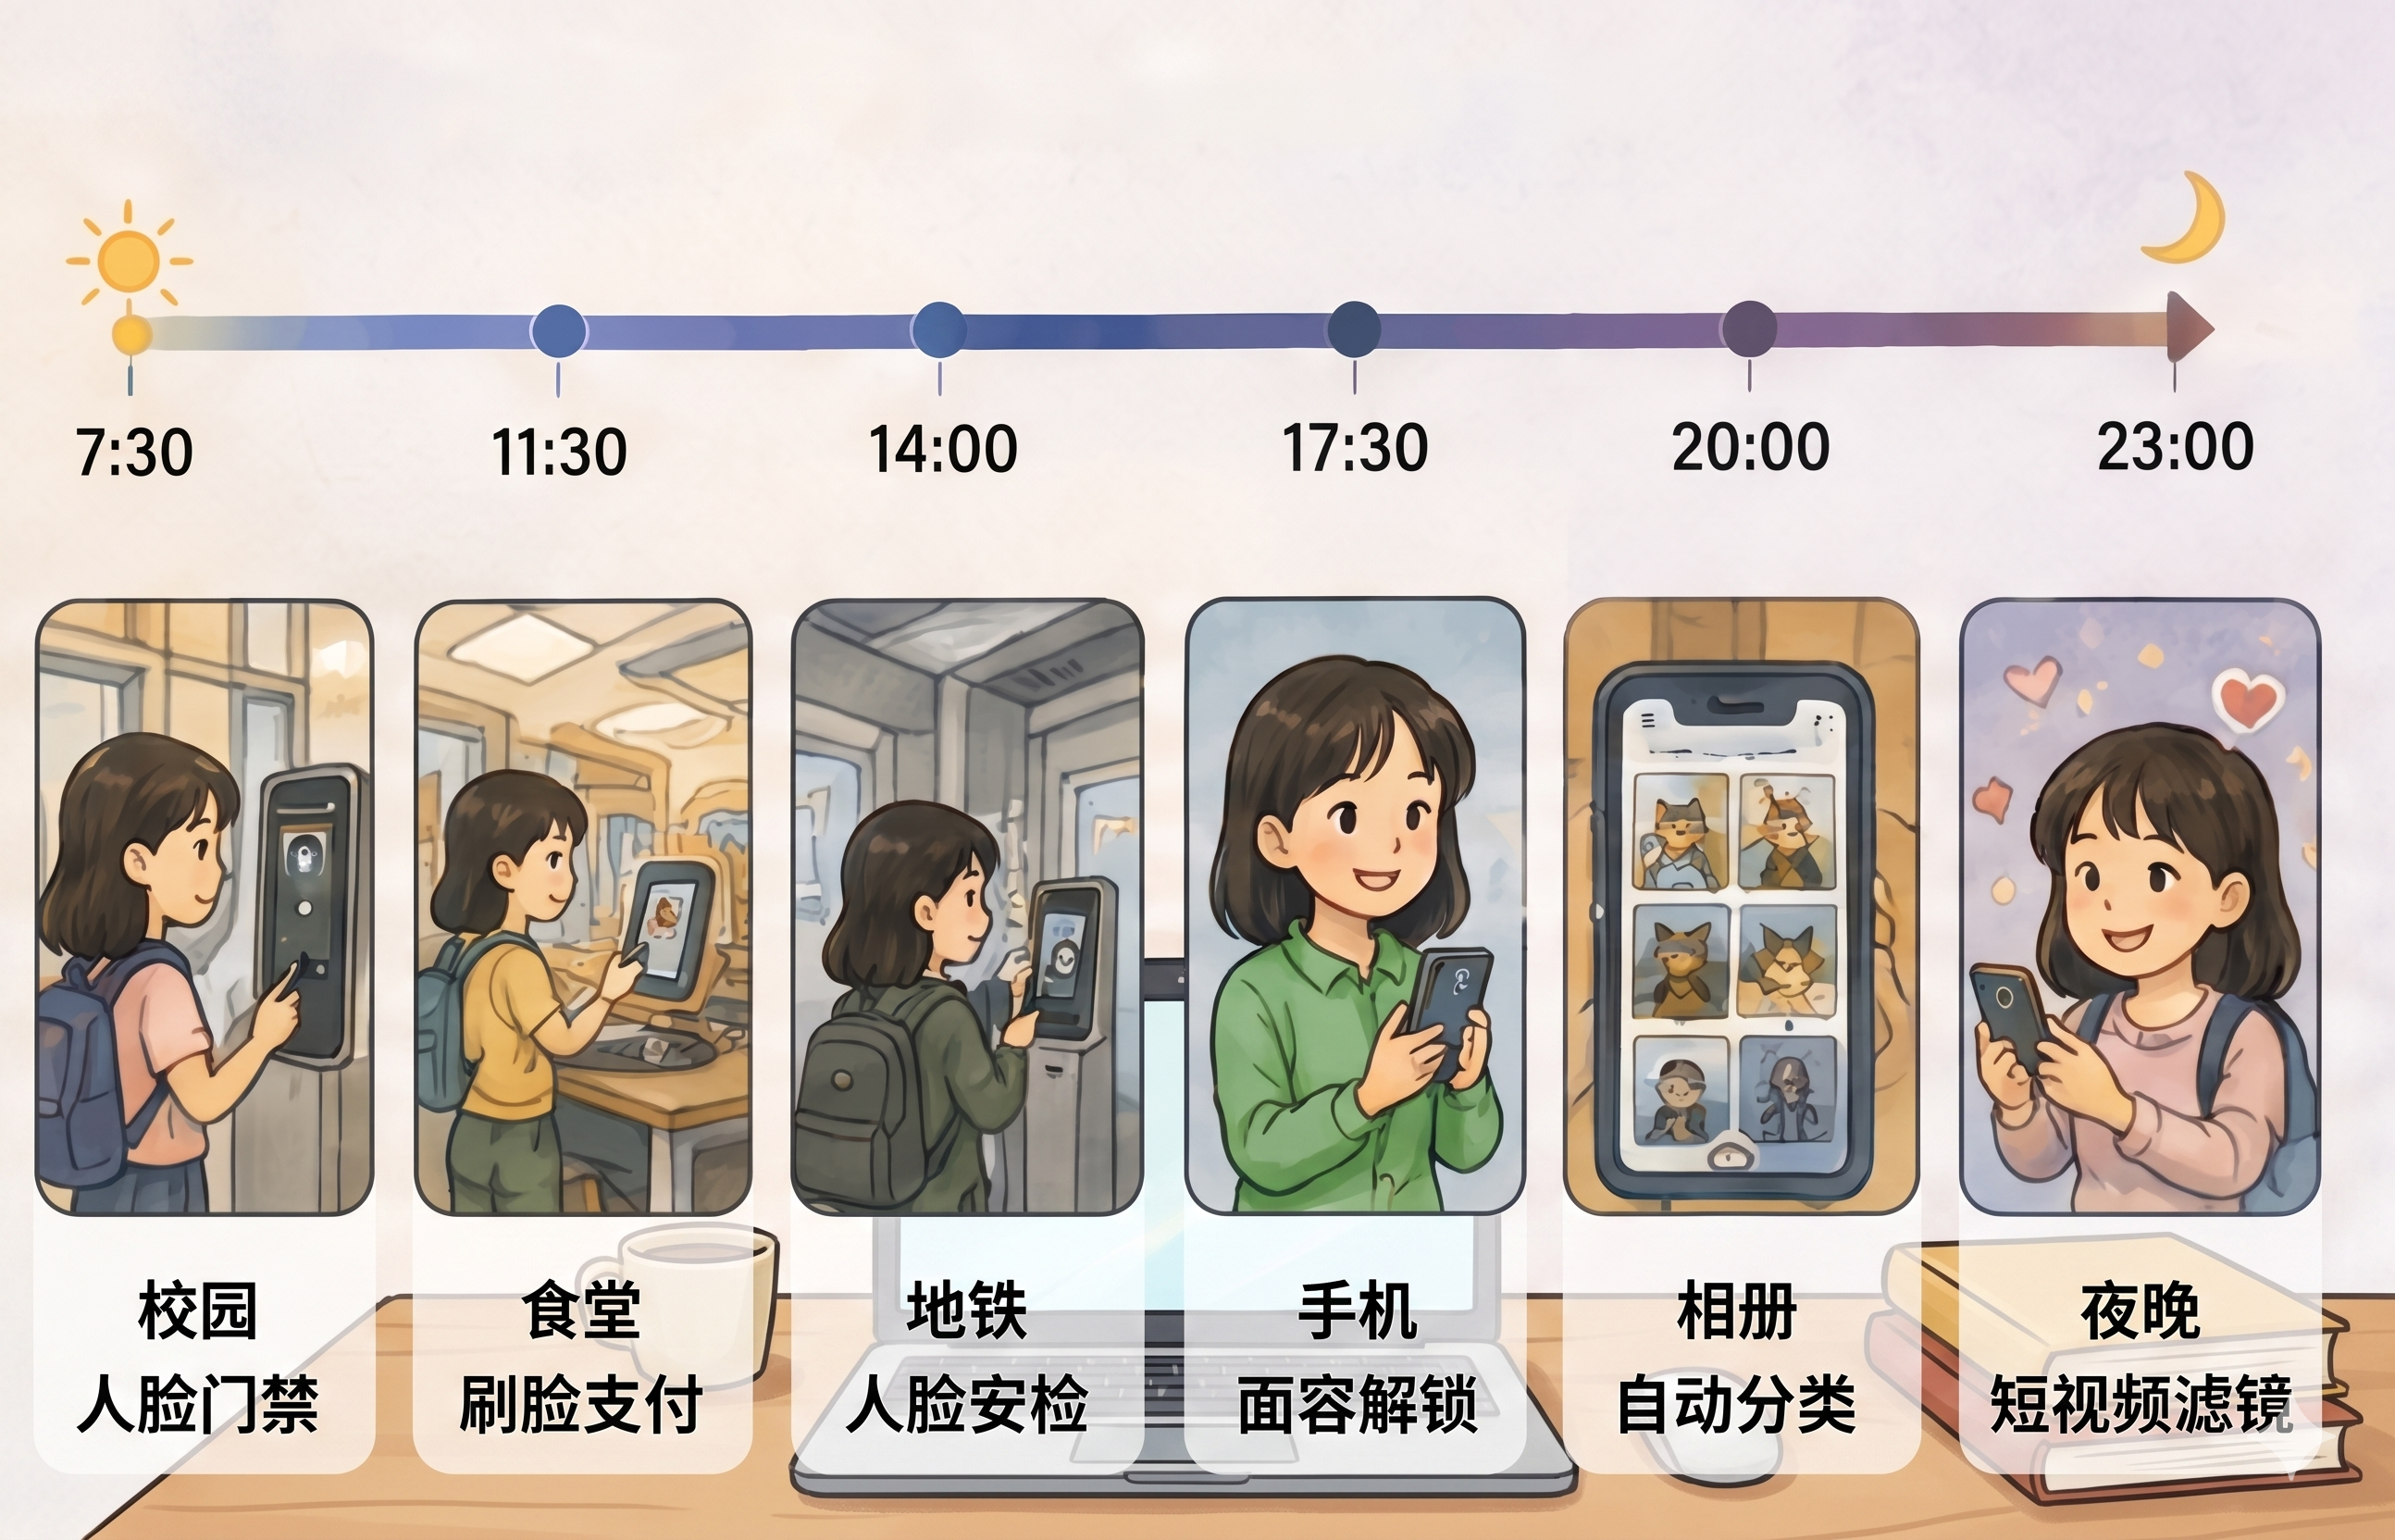
\includegraphics[width=0.88\textwidth]{images_chapter_01-03/2-6.png}
\caption*{\footnotesize\itshape\color{gray!50} 图2-2\quad 推荐系统如何从行为数据中“拼出”用户画像}
\end{figure}

\textbf{生成式AI是怎么“学”的？} 用学书法来类比最好理解。你先是临摹王羲之的字帖，一笔一画模仿他的笔锋。临摹了几百遍几千遍之后，你不仅能把王羲之的字写得很像，还能写王羲之没有写过的字——“鸑”“鷟”这些生僻字王羲之可能没写过，但你写的看起来就像他的笔迹。生成式AI就是那个临摹过几千万张作品的学生。它不是“学会了王羲之的书法”，而是“学会了王羲之写字的统计模式”。

\begin{knowledgebox}
\textbf{扩散模型与GAN——雕塑家与伪造者}

目前AI绘画工具（如Midjourney、Stable Diffusion）背后的核心技术，叫\textbf{扩散模型}。它的思想很巧妙：先给一张照片不断加噪点，直到它变成一片灰色雪花；然后训练AI反着来——从灰色雪花中一层层“去噪”，逐渐还原出清晰的图像。可以把它想象成一位雕塑家，从一块杂乱的石头中逐渐“雕出”清晰的形象。

而\textbf{生成对抗网络（GAN）}则是另一种思路：让两个AI互相“博弈”——一个负责伪造图像，一个负责鉴别真伪。通过数万轮对抗，伪造者最终学会了创作足以乱真的图像，就像一个在一次次被识破中手艺日臻精湛的伪造大师。Deepfake换脸技术就是基于GAN。
\end{knowledgebox}

\textbf{为什么这几年突然爆发？} 三个词：数据、算力、算法。数据——互联网几十年的积累，给了AI几十亿张图片、几万亿字的文本用来“临摹”。算力——GPU等高性能芯片让训练超大模型成为可能。算法——扩散模型、Transformer等新架构让AI终于能高效处理海量数据并提取复杂规律。三个要素同时突破，量变引起质变。

\subsection{生成式AI应用案例}

生成式AI正在让“创作”从少数经过专业训练的人的专属，变成每个有想法的人都可以尝试的事。在设计领域，它快速生成海报、Logo和UI设计方案；在写作领域，它辅助构思大纲、润色语言、生成创意文案；在影视领域，它辅助编剧构思剧情、生成分镜参考图；在音乐领域，它生成旋律框架和伴奏；在文物保护领域，它根据残存数据复原历史文物的原貌；在教育领域，它生成习题、设计课件插图、制作教学视频素材。

下面，我们通过三个来自不同领域的案例，看看生成式AI具体是如何落地应用的。

\subsubsection*{案例1：AI辅助校园短剧编剧——从一个月到一周}

大四学生林语是校园话剧社的编剧。上学期她接到一个任务：为即将到来的校庆创作一部15分钟的短剧，主题是“百年来校园生活的变迁”。

按照传统流程，她需要查校史资料——至少翻阅几十篇文献、老照片集和校友回忆录；构思人物和剧情——要覆盖不同年代，得设计至少三组人物；写剧本——每一幕的对白、动作、舞台提示都要一个字一个字敲出来；修改——初稿出来后至少还要改五六版。整个流程下来，一个月非常紧张。

林语尝试了一个不一样的工作方式。她先是花了半天时间在校史馆和数字档案馆搜集资料，筛选出几个最具代表性的年代切片：抗战时期的西迁岁月、改革开放后的校园复苏、新世纪的信息化浪潮。然后，她将这些资料整理成一份“创作简报”，上传到AI工具。

她输入的指令是：“请根据这份校史资料，为一部15分钟的三幕短剧设计人物关系和剧情框架。三幕分别对应抗战时期、改革开放初期、信息时代。每一幕的时代细节要准确（服装、语言习惯、校园建筑），用表格呈现。”

AI很快给出了结构清晰的框架。更重要的是，它自动补充了林语自己可能花更长时间才能查到的细节——比如抗战时期女生校服的具体样式、80年代校园广播站常用的开场曲。林语在AI框架基础上，用了一天时间打磨对话和动作细节，三天后拿出了完整剧本。

“我不是被AI替代了，”林语后来在剧社分享会上说，“我是被AI加速了。以前一个月做的事，现在一周做完。省下的时间我用来和演员们排练、打磨表演——那些才是AI做不了的。”这个案例的核心启示是：生成式AI的真正价值，不是替代创作者，而是把创作者的精力从繁琐的前期工作中解放出来，投入到真正需要人类判断力、情感和审美的高价值环节中去。

\subsubsection*{案例2：AI帮文物“重现光彩”}

2024年，三星堆博物馆的文物保护团队与AI研究者合作，尝试用生成式AI复原那些残缺严重的出土文物。

以著名的青铜大立人像为例。这尊距今约三千年的青铜像出土时双手缺失，考古学界对手势有多种推测——是持笏？持象牙？持蛇？还是在做一个特定的祭祀手势？各种说法都有文献和同期文物作为依据，但没有人能确定。

AI团队的做法是：让AI学习商周时期同时代青铜器上所有人像手势的造型特征和纹饰规律。在“消化”了大量同时期文物数据后，AI根据铜像手腕的残断面形态和手臂角度，生成了几种不同手势的复原方案。它不提供“唯一正确答案”，而是给考古学家提供更直观的视觉讨论素材。考古团队可以根据每种方案评估其合理性和可能性，缩小推测范围。

另一个更贴近日常的案例是兵马俑的色彩复原。秦始皇陵兵马俑出土时，表面的彩绘层在接触空气后迅速氧化剥落，我们现在看到的陶俑是灰色的。但通过分析残存颜料的化学成分和矿物来源，结合同时期其他出土文物中保存较好的彩绘样本，AI可以生成“刚出土时”兵马俑的色彩复原图——那种两千年前鲜艳生动的彩绘冲击，是任何文字描述都难以传达的。

\subsubsection*{案例3：AI如何帮“数据恐惧症”的文科生做图表}

大二社会学专业学生小徐正在进行一项问卷调查，研究不同年级学生的短视频使用习惯。她回收了三百多份有效问卷，Excel里堆满了原始数据。指导老师要求她在报告里加入数据可视化图表——“至少要有柱状图和饼图”。小徐看到密密麻麻的数字，头都大了。

她对室友抱怨：“我一个文科生，哪会做什么数据透视表啊。”

室友给她推荐了一款AI数据工具。小徐把原始表格上传，在对话框里输入：“请根据这份问卷数据，生成一个对比柱状图，展示不同年级学生每周刷短视频的平均时长，用不同颜色区分年级，标注具体数值。图表标题为‘各年级学生短视频使用时长对比’。”

几十秒后，AI不仅生成了图表，还自动输出了一段文字分析：“大三学生周均短视频使用时长最高（14.2小时），大一最低（9.7小时），整体呈随年级递增趋势。可能原因：随着年级升高，课程压力减轻，可自由支配时间增多。”

小徐看完分析后，又追问了一句：“能帮我再做一个饼图吗？展示每天刷短视频的时段分布——上午、下午、晚上、深夜各占多少比例。”几秒后，第二张图表也完成了。

“原来不是数据分析难，”小徐后来在朋友圈写道，“是我一直用错了工具。AI不是替我做研究，而是帮我把数据‘翻译’成了图表。”这个案例的启示是：生成式AI正在降低专业工具的入门门槛，让更多人能把自己的想法可视化地表达出来。创作者需要的是清晰的表达力和判断力，而不是记住某个软件复杂的操作步骤。

\subsection{AI会取代人类创作者吗}

先看几个翻车现场。你用AI绘图工具画过“手”吗？大概率遇到过“六根手指”或“关节扭曲”的问题。这是著名的老毛病——因为训练数据中手的角度、姿态变化太多，AI很难完全掌握。你读过AI写的诗吗？语句优美，意象丰富，但读完之后总觉得少了点什么。少了什么呢？少了“有人真的经历过这一切”的真实感。AI可以写“我想你就像风走了八千里”，但它从没想过任何人。

\begin{figure}[H]
\centering
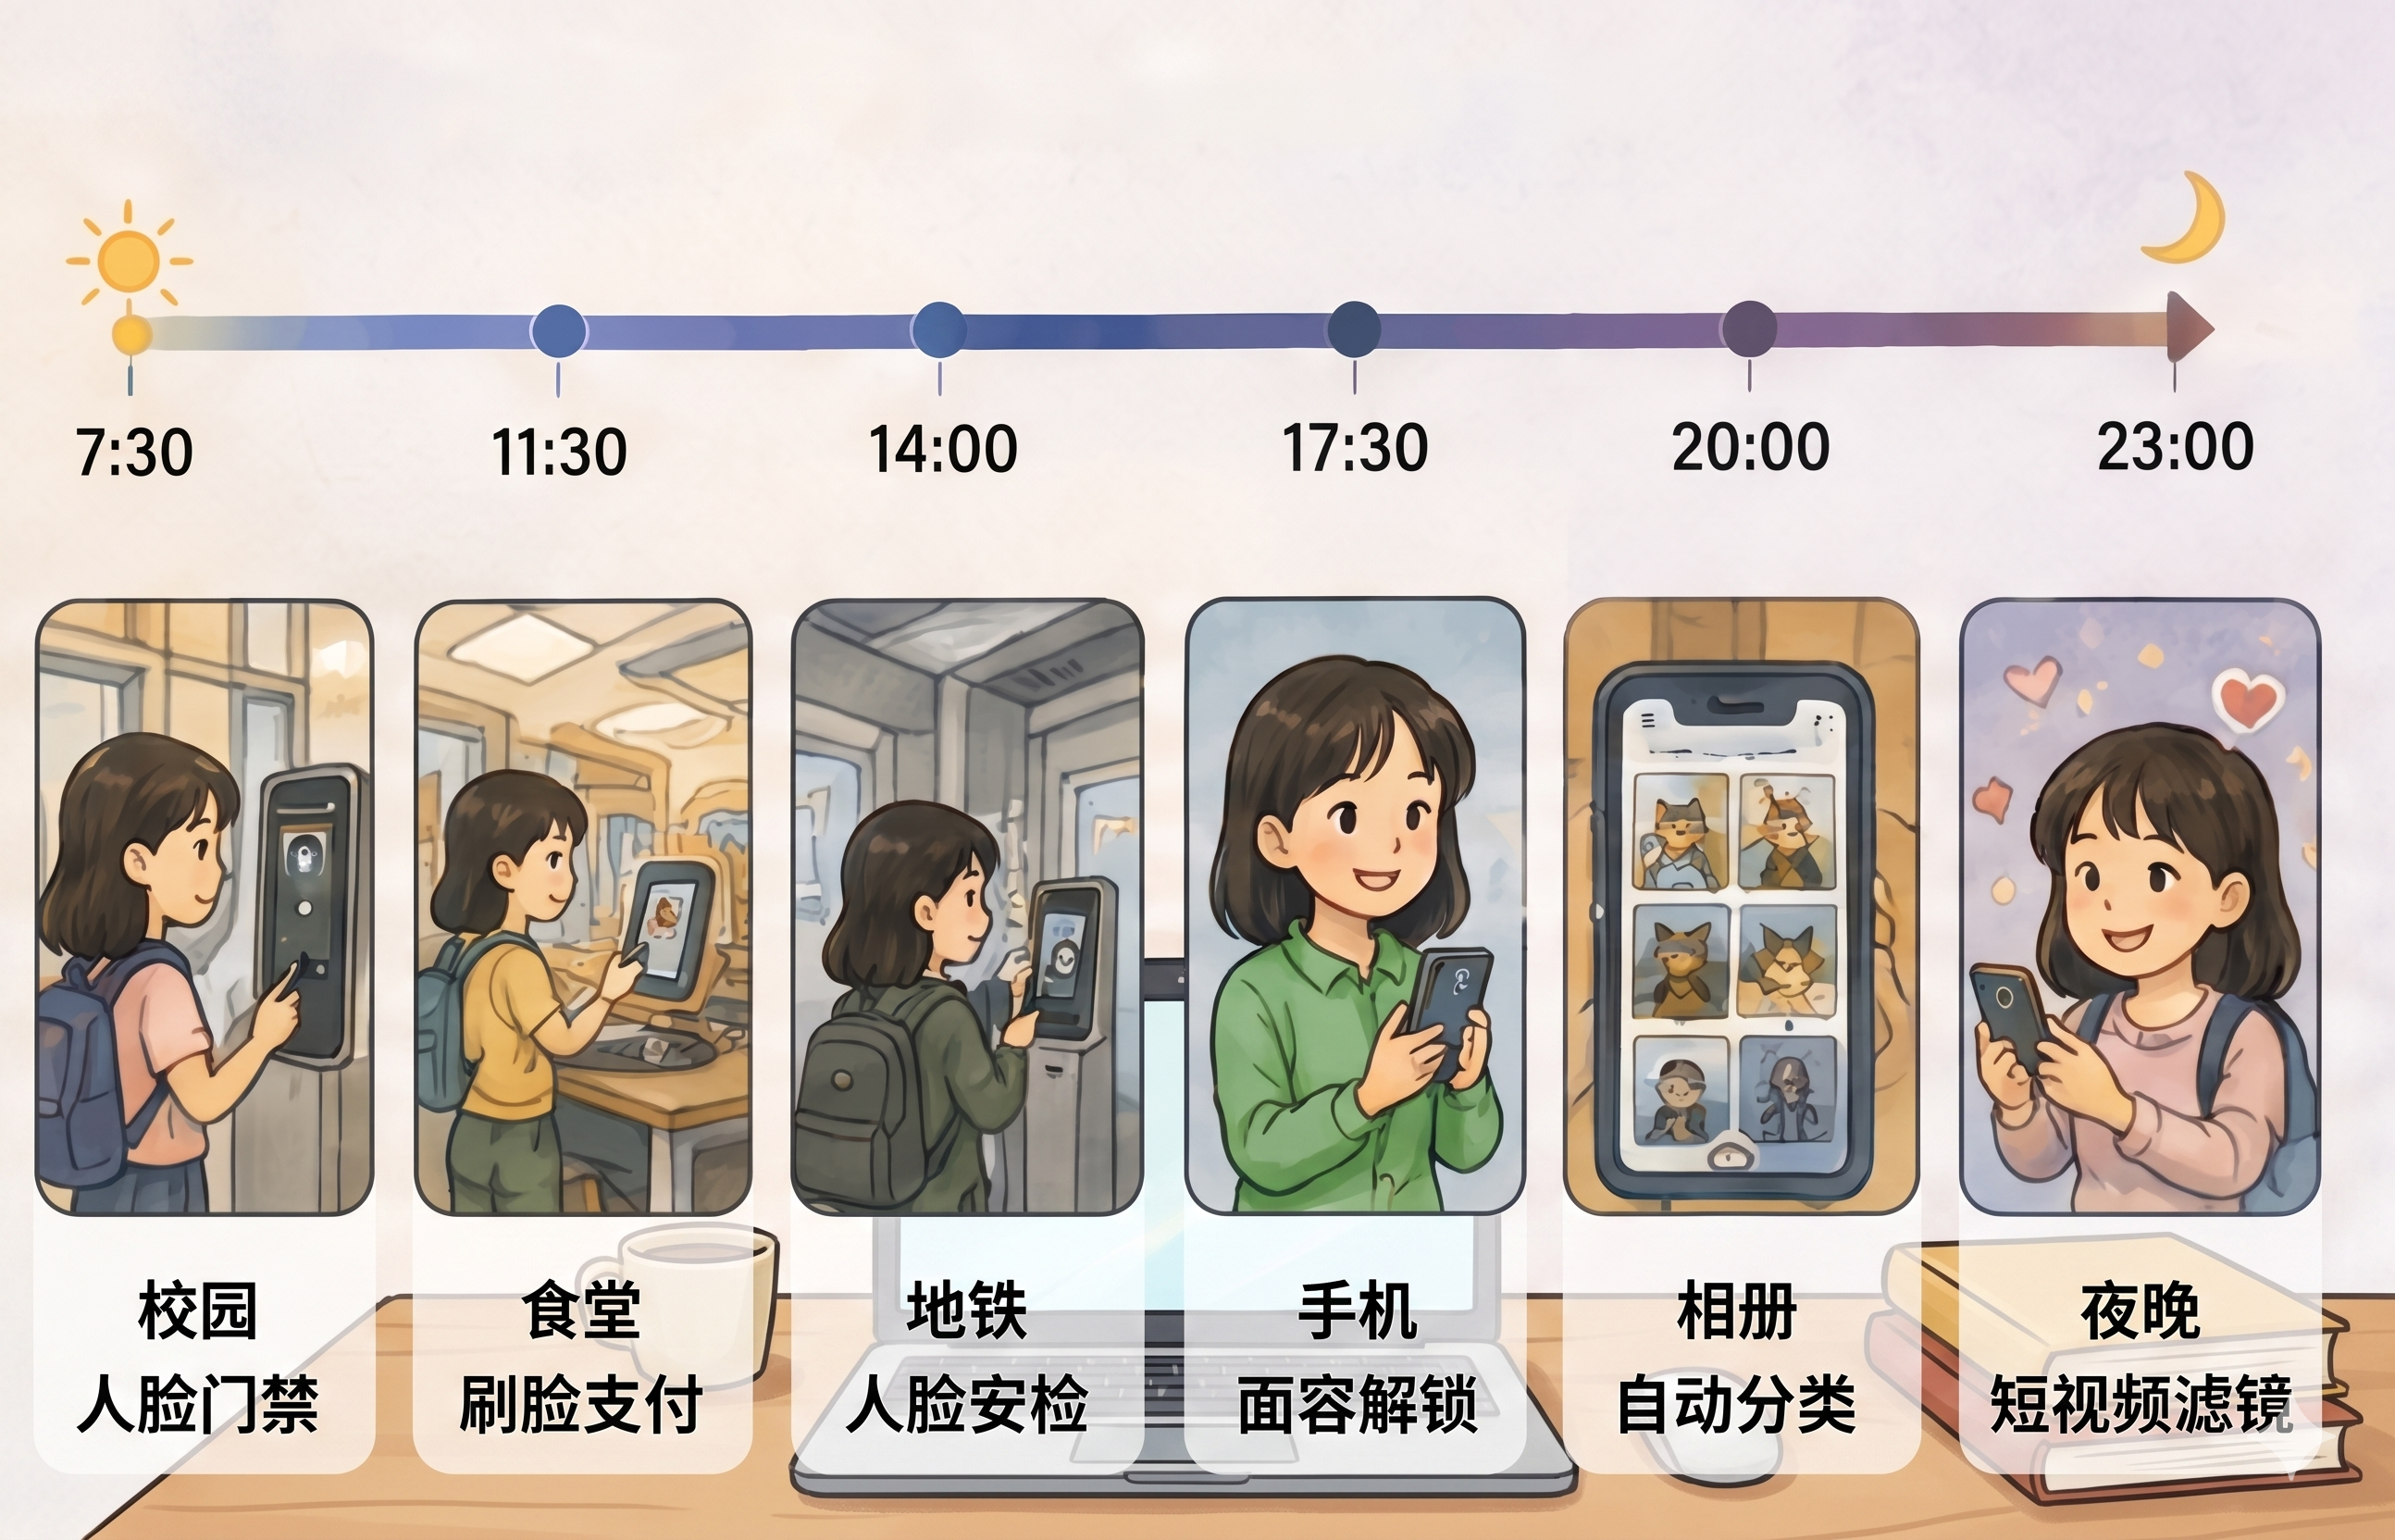
\includegraphics[width=0.88\textwidth]{images_chapter_01-03/2-6.png}
\caption*{\footnotesize\itshape\color{gray!50} 图2-2\quad 推荐系统如何从行为数据中“拼出”用户画像}
\end{figure}

所以，AI到底“创造”了什么？\textbf{AI创造的是“符合人类审美模式的新组合”，而不是“来自真实生命体验的表达”。} 当梵高画《星月夜》时，每一笔扭曲的星空都来自他对世界的独特感知——不是因为他学了一百万张星空画后总结出“星空应该这样画”，而是因为他用那样的方式看世界。AI没有“看世界”的方式。它只是在海量已有作品的基础上，找到了一条“最优重组路径”。

那么，\textbf{AI会取代人类创作者吗？} 答案很可能是：\textbf{AI不会取代人类创作者，但“会用AI的创作者”可能会取代“不会用AI的创作者”。} 就像摄影技术没有取代画家，但永远改变了视觉艺术的方向。AI也是如此。它可能不会“消灭”人类创作，但会改变创作的方式和标准。在AI可以瞬间生成任何风格的图像时，人类画家的价值在哪里？可能在于画出AI生成不出的东西——那些来自真实身体经验、来自具体时空中的独特感知、来自一个有温度的生命对另一个生命的理解。

画笔从毛笔变成钢笔，从钢笔变成数位板。音乐从现场演奏变成录音棚，从黑胶变成流媒体。每一次技术革命，都有人担心“艺术会消亡”。但艺术始终存在，因为人类表达自我的冲动从未消失。AI只是最新的一支“笔”。真正重要的，永远是那个握着笔的人。

\section{AI的能力边界：有所为，有所不为}

走过了机器学习、计算机视觉、自然语言处理和生成式AI四段旅程之后，是时候停下来，把几条线索收拢到一起了。

你会发现一个贯穿始终的共同主题：\textbf{AI在各项能力上展现出的表现都极其强大，但这种强大的本质是“模式识别”和“统计重组”，而不是真正的“理解”和“创造”。}

在本章最后一节，让我们从四个维度来系统讨论AI的边界——它能做什么，绝对不能做什么，以及为什么理解这些“不能”比知道AI“能做什么”更重要。

\subsection{AI为什么会“一本正经地胡说八道”}

2023年春天，大二学生小刘正在赶一篇期末论文。截止时间是第二天中午，他还差三篇参考文献。他灵机一动：让AI直接生成。他输入了详细的提示词：“请推荐5篇关于社交媒体对青少年心理健康影响的近五年学术论文，提供完整的标题、作者、期刊名称和发表年份。”

几秒后，AI返回了五条格式完美的文献——有作者全名，有期刊名称和卷号，有的还附有DOI编号。小刘看都没细看，直接复制粘贴进了论文的参考文献列表。

两天后，老师在课堂上问：“小刘，你这篇论文引用的Smith et al. (2021)，我怎么在期刊数据库里搜不到？”小刘回去一条条核查，发现五篇参考文献里，有三篇完全不存在。作者姓名是真的，期刊也是真期刊，但那些论文从来没有发表过。

\textbf{这就是AI幻觉}——AI生成的内容表达流畅、看似合理，但包含事实性错误或完全虚构的信息。它最危险的地方不是“AI会犯错”——所有工具都会犯错——而是它犯错时看起来和说真话时一样自信。你问它一个它知道正确答案的问题，它语气笃定地回答你。你问它一个它不知道的问题，它同样语气笃定地编造一个。

提示词写得好不好不影响这个问题的存在。因为AI的本质是基于语言规律生成内容，而不是基于事实数据库进行查询。它的目标是“说像人说的话”，不是“说真话”。

所以，\textbf{在任何重要场景中——学业、法律、医疗——AI输出的一切内容，必须经过人工核查。}

\begin{funbox}
\textbf{AI识别坦克的故事——一个关于“伪相关”的经典教训}

在人工智能发展史上，有一个广为流传的经典教训。20世纪80年代，美国军方资助了一个AI项目，目标是让计算机学会自动识别照片中的坦克。研究者收集了大量坦克照片和普通车辆照片作为训练数据，AI在学习后表现出色——在测试集上识别准确率几乎达到100\%。

项目看起来取得了巨大成功。但当系统被部署到实际战场环境中时，它的表现却一落千丈——准确率甚至不如抛硬币。

经过反复排查，研究者发现了一个令人啼笑皆非的问题：训练数据中所有坦克照片都是在阴天拍摄的，而普通车辆照片都是在晴天拍摄的。AI根本没有学会“坦克长什么样”——它只是学会了“阴天=坦克，晴天=普通车辆”。

这个案例完美地说明了AI学习的本质：它不是在“理解”物体是什么，而是在数据中寻找任何能够区分两类样本的统计相关性——无论这个相关性是否真的有意义。这也解释了为什么AI会如此自信地犯错：从统计角度看，“阴天=坦克”和“履带=坦克”一样都是有效的区分规则，AI无法分辨哪个规则是有意义的、哪个是巧合。
\end{funbox}

\subsection{AI也会“戴有色眼镜”}

大二学生阿琳有一段时间特别焦虑。她只是偶然点开了一个健身视频，接下来的几天，整个短视频平台像变了个人：首页全是减肥教程、健身食谱、身材管理经验。甚至有一些视频的标题是“大学女生不管理身材就输了”。

“我只是看了一个健身视频，”阿琳说，“现在它好像觉得我的人生只剩减肥了。”

有人可能会问：这是AI的错吗？从技术上说，AI本身没有“偏见”这个概念。它只是忠实地执行一个指令：\textbf{“推荐用户可能喜欢的内容。”} 但它不知道你点开健身视频是因为假期吃胖了几斤产生的焦虑，它只知道“你点了，我要推更多”。

AI偏见的来源有三个层面：第一，训练数据中的偏见——互联网本身就充满偏见。如果AI学习的招聘数据中CEO大多是男性，AI在筛选简历时就可能更倾向男性。这不是AI“主动歧视”，而是它从数据中学到了“CEO通常是男性”这个统计规律。第二，用户行为造成的偏差——推荐系统会不断强化你已经表现出来的兴趣，让你越看越窄（信息茧房效应）。第三，标签代理偏差——AI常用一些易于测量的特征代替复杂的现实，比如用“点击率”代替“内容质量”，结果就是标题党越来越多。

\textbf{核心认知}：AI并不是绝对客观的。它像一面镜子，反射的是人类社会数据中已经存在的偏见。在很多情况下，AI甚至会放大这些偏见。

\subsection{为什么AI需要人类监督}

2024年，一位独居老人接到电话。“妈，我出事了。”电话那头是儿子的声音。语气急促、恐惧，和平时一模一样。“我开车撞了人，对方家属要赔偿。你先把钱打过来，不要告诉别人，太丢人了。”老人手忙脚乱地翻出存折。就在她准备出门转账时，社区民警入户走访。警察听完描述让她立刻给儿子打个电话确认。电话接通了。儿子正在公司上班，根本没有出车祸。

后来警方调查发现，那通电话不是真人打的。犯罪分子从社交平台上获取了老人儿子的语音数据，使用\textbf{AI语音克隆技术}复制了他的声音。只需要几秒钟的语音样本，AI就能复制一个人的音色、语调、停顿和情绪表达。

\begin{knowledgebox}
\textbf{AI语音克隆与Deepfake——技术的双面刃}

\textbf{AI语音克隆}是指利用AI技术，从几秒钟到几分钟的真人语音样本中提取说话人的音色、语调、停顿和情绪特征，然后生成该说话人从未说过的全新语音内容。其原理类似于生成式AI根据文字描述生成图像——只不过生成的是声音波形。

\textbf{Deepfake}（深度伪造）是“Deep Learning”和“Fake”的合成词，泛指利用深度学习技术伪造视频、音频或图像的技术。换脸视频是最典型、最早引起公众关注的Deepfake应用。Deepfake具有双重属性——既可以用于电影特效、历史人物复原等正当用途，也可能被用于制造虚假新闻和电信诈骗。目前各国正在逐步建立针对Deepfake的法律监管框架。
\end{knowledgebox}

这个故事虽然令人毛骨悚然，但它并不是孤例。随着AI技术越来越强大，滥用AI的门槛也在降低：有人将个人隐私数据上传到不安全的AI平台造成泄露；有人用AI批量生成虚假新闻操纵舆论；Deepfake换脸技术被用来伪造公众人物讲话视频。

请注意：AI本身没有善恶观。它不知道“克隆别人的声音去骗钱”是坏的。它只是一个工具。就像一把刀——可以做一顿美味的晚餐，也可以成为凶器。刀没有善恶，关键在于握刀的人。正因为AI没有道德判断，\textbf{人类监督才必不可少。} 无论AI技术多么先进，最终仍然需要人类制定使用规则、审核产出内容、承担相应责任。

\subsection{AI真正缺少什么}

深夜一点半，大三学生小周睡不着。他刚刚查出期末成绩——专业课考砸了。他不敢告诉父母，不敢告诉同学，一个人窝在被窝里。翻遍通讯录，不知道该找谁说话。犹豫了很久，他打开手机上的AI聊天应用，打了一行字：“我考砸了，很难受。”

AI很快回复：“听到你考砸了，我能理解你现在的心情。一次失败不代表什么，你付出的努力不会白费。”那些话温柔、理性、充满耐心。甚至比一些现实中的人还会安慰人。

小周回了一大段，讲了考试有多难，讲了他复习到凌晨两三点的那些夜晚，讲了看到成绩时手抖的感觉。AI每一条都认真回复。到了凌晨三点，小周打出最后一句：“谢谢你，我感觉好点了。”然后沉沉睡去。

但他没有问自己一个问题：\textbf{“它真的理解我了吗？”}

AI做对了什么？它识别出了“考砸了”和“难过”之间在语言上的关联——因为在训练数据中，这两个词大量共现。它识别出这是一段需要安慰的对话——因为对话的语义模式符合“倾诉-安慰”的场景特征。它能生成符合“温暖、理性、不评判”风格的回复。

但它不能做什么？它不知道“考砸了”对一个具体的人意味着什么。它不会心疼。它没有经历过“努力之后失败”的苦涩——它只是识别出你的文字里有这种情绪的语义表征。它不会在你睡着后还在想“那个学生不知道有没有好起来”。当你关掉对话窗口，这段对话对AI来说就结束了，就像你关掉了一个文档。

\begin{figure}[H]
\centering
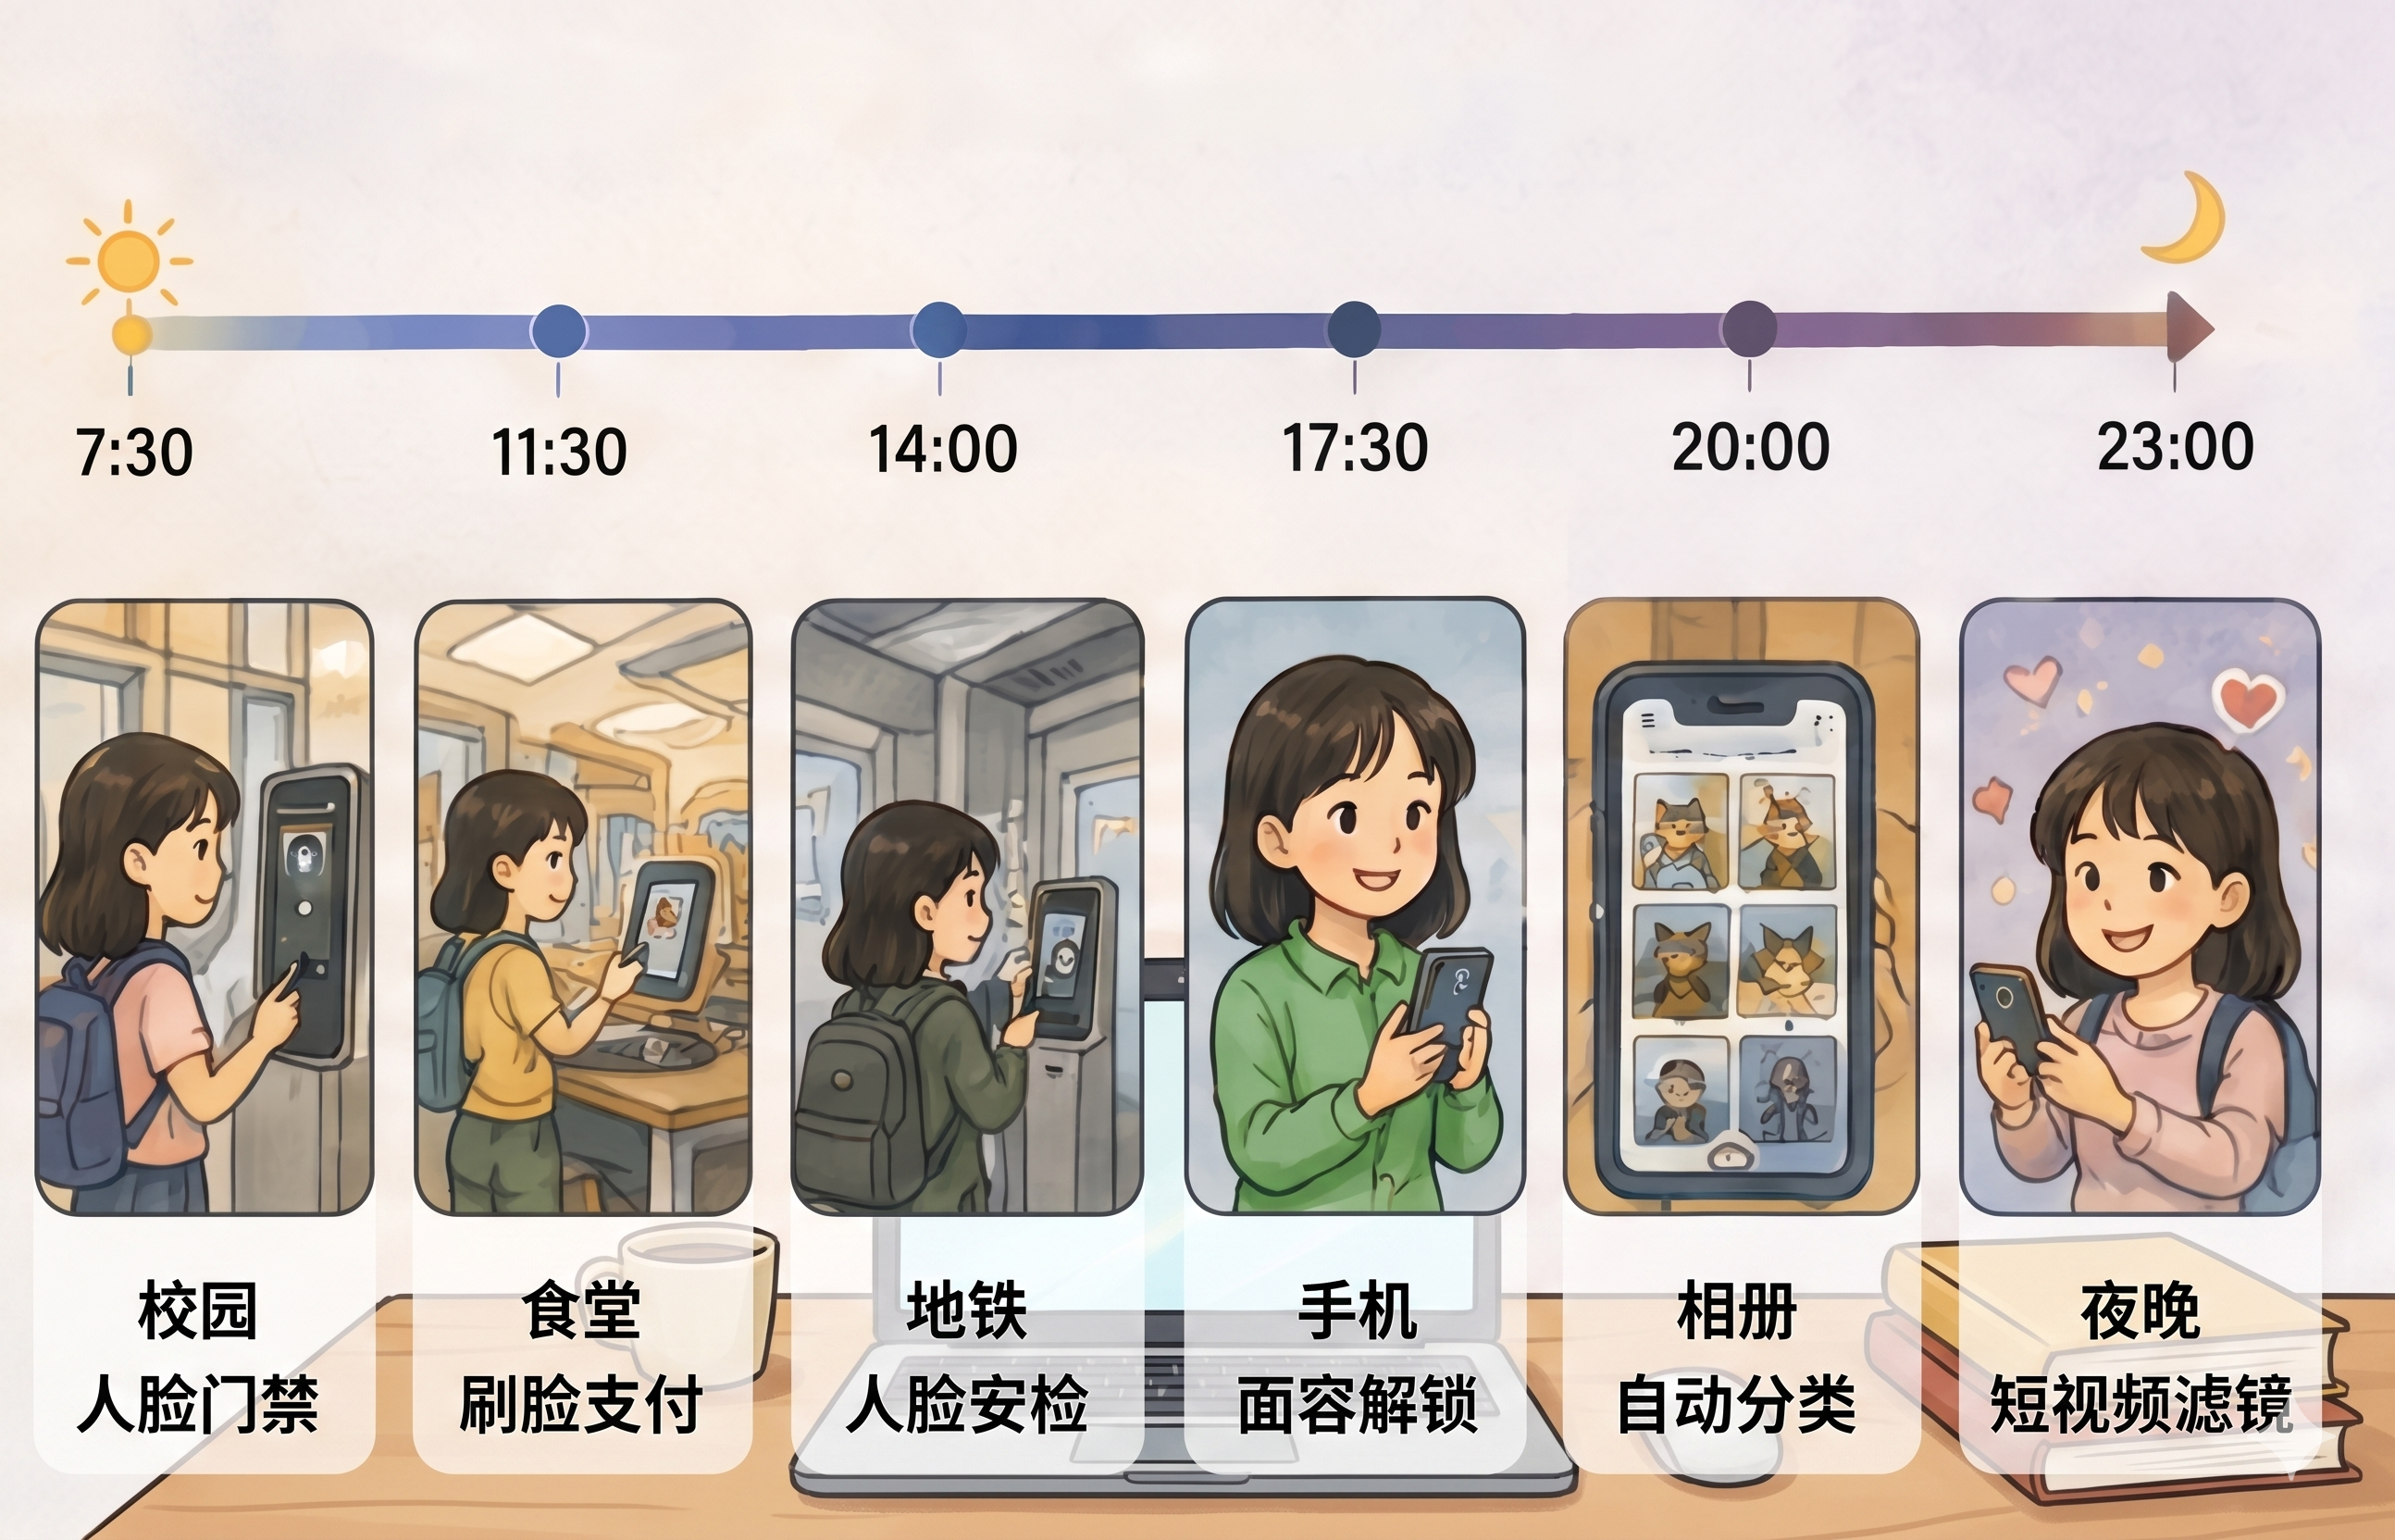
\includegraphics[width=0.88\textwidth]{images_chapter_01-03/2-6.png}
\caption*{\footnotesize\itshape\color{gray!50} 图2-2\quad 推荐系统如何从行为数据中“拼出”用户画像}
\end{figure}

这就是AI最根本的边界。它可以在几秒钟内生成一篇“关于母爱”的感人散文，但它从未有过母亲。它可以模仿一个作家的所有风格特征写出一篇“新作”，但它不知道那位作家在创作时的精神状态。它可以分析大量数据做出商业决策建议，但它无法像人类一样进行道德判断和价值选择。

\textbf{AI不会成为“人”，因为它没有第一人称体验，没有真正的意识和自我觉察，无法进行道德选择和承担后果，没有真实的欲望和意图。} 它只是一面极其强大的镜子——反射人类语言、人类图像、人类创造中的所有模式。但它不是光源本身。

\section*{本章小结}
\addcontentsline{toc}{section}{本章小结}

这一章，我们从四个维度了解了AI如何认识世界。

我们了解了\textbf{机器学习}——AI从数据中总结规律，拦截诈骗短信、预测天气、辅助诊断疾病，但它只是在做概率计算，不是在思考。

我们了解了\textbf{计算机视觉}——AI能从像素中提取特征，识别物体、人脸、路况，但它看到的只是数字和模式，不是意义和情感。

我们了解了\textbf{自然语言处理}——大语言模型让AI变得“能说会道”，但它的语言能力来自海量文本的概率学习，它不理解自己说的话。

我们了解了\textbf{生成式AI}——AI能画画、写文章、做音乐，但它的“创作”本质是模仿重组，而不是真正的灵感迸发。

最后，我们系统地审视了AI的边界：它会一本正经地编造事实，它会忠实复制人类的偏见，它可能被滥用，它永远无法成为有意识、有情感、有道德感的“人”。

\textbf{AI不是魔法，也不是魔鬼。} 它是人类创造的工具——一个极其擅长发现规律、处理信息、生成内容的工具。它的强大在于数据处理的规模和速度，它的局限在于没有意识、没有情感、没有真正的理解能力。

理解了这些，你就拥有了面对AI最重要的东西：\textbf{不是技术能力，而是认知框架。} 你不会把它当神崇拜，也不会把它当鬼恐惧。你会把它当作一个强大的工具——理解它的能力，清楚它的边界，学会和它协作，同时承担作为使用者的判断和责任。

而在理解了AI能做什么、不能做什么之后，一个更实际的问题自然浮现：既然AI是这样工作的，那我们该怎么和它高效协作？怎么写好提示词？怎么让AI从“回答问题”变成“帮你做事”？这就是下一章要回答的问题。

% ============================================================
% 第3章 提示词工程与智能体系统(扩充版，目标~50页)
% ============================================================

\chapter{提示词工程与智能体系统}


\section*{}
% \addcontentsline{toc}{section}{本章导览}
上一章我们了解了AI如何学习和理解世界，从机器学习到深度学习，从卷积网络到注意力机制。但这些能力要真正为我们所用，离不开人与AI的有效对话。

学期末，小林面临一门课程论文的截止压力。他需要完成一篇关于深度学习在医学影像中的应用的4000字综述。第一次，他打开AI对话框输入了“帮我写一篇论文”，AI只回复了1200字的泛泛之谈。第二次他限定了字数，但引用的都是2020年之前的文献。直到第三次，他仔细拆解了任务，设定了角色、分步给出指令、约束了输出格式，AI终于产出了一篇结构清晰、引用规范的完整综述。同样的AI、同样的话题，只是提问方式不同，结果天差地别。
读完本章，你将找到这些问题的答案。在开始之前，先带着以下几个问题来阅读：

\begin{itemize}
\item \textbf{为什么同一个AI、同样的任务，不同的提问方式会得到天差地别的结果?} 提示词的词法与语法决定了AI理解任务的起点。
\item \textbf{如何让AI按照特定的角色和思维框架来回答问题?} 角色设定不是扮演游戏，而是在AI的知识空间中划定注意力边界。
\item \textbf{AI为什么会忘记前面说过的话?如何管理它的记忆?} 上下文窗口是AI的短期记忆，善用它才能保证连贯性。
\item \textbf{怎样让AI在复杂推理中少犯错误?} 思维链让AI把心算变成笔算，每一步透明可见。
\item \textbf{能否把调教好的提示词保存下来反复使用?} Skill蒸馏将零散的成功经验固化为可复用的能力模块。
\item \textbf{AI如何从你问它答升级为自主完成任务?} 智能体通过感知、规划、工具调用和反馈调整构建执行闭环。
\item \textbf{当多个AI分工协作时，它们如何沟通、如何避免冲突?} 多智能体系统需要主从、议会或市场等组织模式来协调。
\item \textbf{当AI走出屏幕进入物理世界，会面临哪些全新的安全挑战?} 具身智能带来的实时性、隐私权限和责任归属问题。
\end{itemize}

\begin{center}
\textcolor{gray!70}{\*\ \ \*\ \ \*}
\end{center}
\vspace{12pt}

\newpage
% ============================================================
\section[提示词的文法与设计]{\textbf{提示词}\footnote{提示词(Prompt)：用户向AI输入的自然语言指令，引导AI生成特定类型的输出。}的文法与设计}
% ============================================================

\begin{sectionkeypoints}
\item 了解提示词的词法和语法基本规范，理解动词、形容词和约束条件对输出类型与风格的决定性作用
\item 掌握角色设定的本质与五大要素，理解完整的身份、经验、风格、框架和约束对输出稳定性的影响
\item 掌握上下文窗口的概念及其管理策略，理解背景注入、示例引导和格式说明三种控制方式
\item 理解思维链推理的核心思想及零样本思维链、思维树、反思链三种变体的适用场景
\item 掌握提示词综合模板的结构，理解角色设定、分步任务、格式要求和约束条件的整合方法
\item 理解结构化输出的重要性，掌握表格、JSON、Mermaid等常见输出格式的约束技巧
\end{sectionkeypoints}



现在，让我们继续回到小林的例子。有了前面的失败经验，他开始有意识地设计提示词的每一步细节。他这样输入：

\begin{userbox}
你是一位医学影像专业的研究生。请帮我完成一份关于“深度学习在肺结节CT影像诊断中的应用”的文献综述。
第一步搜索近五年(2021-2025年)该领域的核心文献；
第二步按以下框架组织内容：常用深度学习模型(CNN、U-Net、Transformer)、公开数据集(LUNA16、LIDC-IDRI)、关键性能指标(敏感度、假阳性率)、当前局限与未来方向；
第三步为每个部分配2-3个代表性研究的引用；
第四步用表格比较不同模型在LUNA16数据集上的表现。
语言风格保持学术性但不晦涩。
\end{userbox}

\begin{aibox}
\textbf{文献综述：深度学习在肺结节CT诊断中的应用}

\textbf{1. 常用深度学习模型}

CNN类模型(ResNet、DenseNet等)是肺结节检测的基础架构，在LUNA16上取得了92.3\%的敏感度。U-Net及其变体在分割任务中表现突出，Dice系数可达0.89。Vision Transformer在大规模数据上表现优于传统CNN。

\textbf{2. 性能对比}

\begin{formalTable}[H]
\caption{不同模型在LUNA16数据集上的性能对比}
\label{tab:ch3_01_model_performance}
\begin{tabular}{c c c}
\toprule
模型 & 敏感度 & 假阳性率 \\ \midrule
3D CNN & 94.2\% & 1.0/scan \\
U-Net+ResNet & 95.8\% & 0.8/scan \\
Swin Transformer & 96.5\% & 0.6/scan \\ \bottomrule
\end{tabular}
\end{formalTable}

\textbf{3. 当前局限：}小样本泛化能力不足，临床验证研究有限。
\end{aibox}

这一次AI产出了一篇4000多字、结构清晰、引用了十五篇文献的综述。小林拿到AI初稿后，又花了一小时用“临床验证方面能不能增加一些多中心研究的数据”进行第二轮追问，AI补充了三篇2024年的临床试验文献，最后又用了30分钟调整格式和补充个人见解。小林总共约两小时完成了一篇高质量综述。
由此可以得出第一条原则：提示词不是随便问问，而是一种需要学习的沟通语言。

\begin{funbox}
\textbf{Prompt一词的来历。} 

今天AI领域使用的提示词(Prompt)一词，源头可追溯至拉丁语“promptus”，本意为“使准备好、使就绪”。在计算机科学早期，终端界面上的提示符就被称为prompt：它静静地闪烁在屏幕上，等待用户输入指令。2022 年底，随着 ChatGPT 等大语言模型的发布，这个原本属于命令行界面的词汇被赋予了全新的含义：从“系统等待你输入”变成了“你引导系统输出的”魔法语言。历史就这样完成了对同一个词的双重解读。
\end{funbox}

\subsection[词法语法与基本规范]{\textbf{词法}\footnote{词法(Lexicon)：提示词中词汇的选择和使用，包括动词、形容词等关键词类的运用。}\textbf{语法}\footnote{语法(Syntax)：提示词中句子的组织结构和信息排列顺序。}与基本规范}

小林打开AI对话框，最直接的问题就是：该说什么?怎么说?
他和很多人一样，以为提示词就是随便问问，但事实远非如此。提示词有自己的词法：选择合适的词汇；也有自己的语法：组织句子的结构。理解了这两个层面，就能从随便问问升级到精准指挥。 如图\ref{fig:ch3_3_1}所示，结构化提示词通过明确的角色设定、分步任务和格式约束，相比简单一句话提问能获得结构更清晰、内容更丰富的回答。

\begin{figure}[H]
\centering
\BookFigureImage{./images_chapter_01-03/3.1.png}
\caption{一句话提示词与结构化提示词对比}
\label{fig:ch3_3_1}
\end{figure}



\subsubsection*{\textbf{•词法的核心要素}}

词法：选对词。提示词中最关键的词类就是动词。动词决定了AI将用户当作什么角色来服务，也决定了输出内容的类型。例如，同样是问光合作用的知识，如果用不同动词效果完全不同。对AI提问“请描述一下光合作用”，得到的可能是教科书式描述；用“用表格对比C3和C4植物”则会得到结构清晰的对比表格。如图\ref{fig:ch3_3_2}所示，使用“描述”、“对比”、“分析”等不同动词会引导AI产生截然不同的输出格式和信息密度。

\begin{figure}[H]
\centering
\BookFigureImage{./images_chapter_01-03/3.2.png}
\caption{不同动词的输出效果对比}
\label{fig:ch3_3_2}
\end{figure}

再看一个反面案例：如果像这样提问“看一下这个数据”，AI会输出含糊评论，因为它不知道用户要分析、总结还是确认，如下图所示。\par \begin{userbox}
看一下这个数据。

\end{userbox}

\begin{aibox}
好的让我看看。这份数据记录了三个组别的测量结果看起来分布比较均匀。对照组数据波动较大实验组相对稳定。总体来看实验结果有一定参考价值但需要进一步分析。
\end{aibox}

AI不知道用户要分析、总结还是确认。好的提示词应该明确指定任务，并通过
形容词控制风格和深度。如果详细地让AI展开论述，AI可能会写出一整页；如果让AI简洁地提炼要点，通常输出3-5个点；如果让AI以学术风格回答，则会引用文献保持严谨用语；如果让AI以通俗风格回答，则会用比喻和例子解释复杂概念。约束条件的词同样重要：“近五年的文献”限定了时间范围，“中国学术界的观点”限定了地域，“APA格式”指定了引用规范。 

\subsubsection*{\textbf{•语法的组织结构}}

语法：排好序。提示词不是把信息堆砌在一起就行了，句子的组织方式同样重要。

第一种是总分总结构，先给出整体目标，再展开具体任务，最后总结要求，让AI先理解大局再处理细节，输出更有条理；第二种是递进结构，先提供背景信息，再逐步深入，每一步都建立在前一步的基础上；第三种是对比结构，要求AI同时对比多个对象，AI通常在表格中呈现结果，信息密度高、一目了然。 如图\ref{fig:ch3_3_3}所示，总分总、递进和对比三种语法结构各有特点，合理的结构组织能让AI输出更有条理。

\begin{figure}[H]
\centering
\BookFigureImage{./images_chapter_01-03/3.3.png}
\caption{提示词的三种语法结构对比}
\label{fig:ch3_3_3}
\end{figure}





\subsubsection*{\textbf{•常见错误与防范}}


常见的提示词错误有三种。第一种是过于模糊：只说“帮我写点东西”，AI不知道题材、长度、风格，输出随机且几乎不可用。第二种是信息过载：把所有要求一次性塞进一句话，AI无法区分优先级，输出混乱，应该分段落、分要点组织。第三种是缺少约束：不提限制条件，AI可能用2018年的数据(如果需要2025年的数据)，或者用美国市场的案例(如果需要中国市场的案例)。

在对比实验中，小林给AI完全相同的底层问题，但使用不同质量的提示词。结果显示：结构化提示词获得有效回答的概率比简单提问高出约三到四倍。写好提示词不是锦上添花，而是使用AI的必需技能。
\begin{funbox}
\textbf{提示词的两位老祖宗：SHRDLU与ELIZA。} 

1960年代末，MIT接连诞生了两个对AI对话影响深远的程序。一个是约瑟夫·魏泽鲍姆的ELIZA：它通过简单的模式匹配模拟心理治疗师，当用户说“我觉得很沮丧”时，它会回应“你为什么会觉得沮丧?”。尽管魏泽鲍姆明确声明ELIZA没有任何理解能力，许多用户仍然向它倾吐内心最深处的秘密。另一个是特里·维诺格拉德的SHRDLU：它生活在一个虚拟积木世界中，能理解“把那块绿色的方块放到红色棱锥上面”这样的指令。ELIZA教会了我们：人们容易被“听起来像在理解”的程序所迷惑；SHRDLU则证明了：真正的理解需要明确的指令和可执行的分解。今天写提示词时，应当从SHRDLU那里学会精确分解任务，同时警惕ELIZA效应：不要假设AI真的理解我们，而要精确描述我们想要什么。
\end{funbox}

\subsection[角色设定与语义框架]{\textbf{角色设定}\footnote{角色设定(Role Setting)：在提示词中为AI指定身份、能力和行为方式的技巧。}与语义框架}

小林发现，AI默认的回答风格是百科全书式的，中立、全面、不带倾向。但在很多场景中，需要的不是一个百科全书，而是一个特定角色。 如图\ref{fig:ch3_3_4}所示，同一问题下，设定不同角色(专家、教师、顾问)会使AI的回答在知识侧重和表达风格上产生明显差异。

\begin{figure}[H]
\centering
\BookFigureImage{./images_chapter_01-03/3.4.png}
\caption{不同角色设定的回答差异}
\label{fig:ch3_3_4}
\end{figure}

\subsubsection*{\textbf{•角色设定的本质与要素}}


角色不是AI真的变成了那个人，而是为AI提供了一个思维框架：限制它的知识范围、调整它的表达方式、指定它的判断标准。可以把角色理解为一个知识过滤器：当AI接收到角色指令后，它会在庞大的参数空间中激活与该角色相关的知识子集，同时抑制不相关的知识。

这个机制解释了为什么同一问题设定不同角色会得到截然不同的回答：不是AI在扮演，而是它真的从不同的知识子集中提取信息、用不同的表达方式组织语言。
\begin{funbox}
\textbf{从注意力到角色设定：划定AI的知识边界。} 

理解角色设定为什么要先理解注意力?从第2.4节可知，注意力机制是AI理解信息的核心：它决定模型看哪里。角色设定的本质，正是利用这个机制为AI划定注意力的边界：当告诉AI“你是一位资深内科医生”时，是在指示它的注意力聚焦于医学知识路径，抑制无关信息。当告诉AI“请用SWOT框架分析”时，是在约束它的注意力在优势→劣势→机会→威胁四个维度的分配方式。


\end{funbox}

当告诉AI“你是一位资深面试官”时，模型会激活与面试相关的知识体(常见的提问模式、评价标准、沟通话术)，同时抑制其他不相关的知识。

角色设定的应用实例：
假设我们要让AI完成几项不同的任务。如果告诉AI“你是一位资深面试官，正在招聘一名前端工程师，请根据这份简历列出5个技术面试问题并附上期望回答要点”，AI输出的问题会集中在JavaScript、React、性能优化等技术领域，语气专业且具有甄别性。如果告诉AI“你是一位大学英语四级考官，请生成一篇四级阅读理解短文并附带5道选择题”，AI会自动调整词汇难度至CET-4水平，设计干扰项合理的选项。如果告诉AI“请你扮演一位历史学教授，解释唐朝安史之乱的起因和影响”，AI会以学术口吻回答，引用史料并给出不同史学流派的观点对比。

角色不只是身份标签，更需要配套能力描述、语气风格和约束条件。例如：

\begin{lightquote}
“你是一位有15年经验的儿科医生，擅长用通俗易懂的语言向家长解释病情。在给出诊断建议前，请先列出所有可能性并按概率排序。不要使用专业术语，除非给出对应的通俗解释。”
\end{lightquote}

这个角色设定包含了身份(儿科医生)、经验年限(15年)、沟通风格(通俗易懂)、思考框架(先列可能性再排序)、约束条件(术语需附带解释)。越完整的角色设定，AI的输出越稳定。 如图\ref{fig:ch3_3_5}所示，有效的角色设定包含身份、经验年限、沟通风格、思考框架和约束条件五大要素，要素越完整输出越稳定。

\begin{figure}[H]
\centering
\BookFigureImage{./images_chapter_01-03/3.5.png}
\caption{有效角色设定的五大要素}
\label{fig:ch3_3_5}
\end{figure}

反面案例：角色设定不足。有些角色设定看似给出了身份，实际上信息不足。例如，如果只说“你是一位专家，帮我分析一下这个市场”，AI不知道是哪方面的专家、什么级别的专业度、以什么立场来分析。又如，“请以CEO的口吻回答”只有身份没有配套的能力描述，AI虽然语气像CEO，但分析深度可能不够。


\subsubsection*{\textbf{•语义框架的应用}}
除了角色设定，还可以指定思考框架，要求AI按特定的方法论分析问题。例如SWOT框架要求从优势、劣势、机会、威胁四个维度展开评估；金字塔原理要求先给出核心结论，再逐层展开论据，每个论据配具体数据支撑；5W1H框架则要求从谁、什么、何时、何地、为何、如何六个角度分析问题。


\subsubsection*{\textbf{•多角色切换策略}}
一个强大的技巧是在同一对话中切换角色。先让AI扮演“严苛的审查者”挑出方案的漏洞，再让它扮演“乐观的推行者”提出实施建议。 小杨在准备课题汇报时，先让AI扮演同行评审专家，逐条质疑研究方案的方法论合理性，AI指出了3个潜在的设计缺陷；然后切换角色，让AI扮演跨学科专家，从数据分析角度重新评估方案，AI又补充了两个之前忽略的交互效应因素。通过两个角色的交叉审视，小杨的最终方案既规避了风险，又抓住了机遇。这种多角色分析能让决策更全面，不需要换人，只需要换提示词。

\subsection{上下文控制与作用机制}

小林有时会遇到这样的情况：明明刚才已经和AI说过某件事了，过了一会儿再问，它好像完全忘了。这不是AI的记忆力差，而是因为一个限制：\textbf{上下文窗口}\footnote{上下文窗口(Context Window)：AI模型一次能处理的文本总量上限，超出部分会被截断或遗忘。}。 如图\ref{fig:ch3_3_6}所示，上下文窗口中靠近开头和结尾的信息具有最高的注意力权重，AI对中间部分的记忆相对较弱。

\begin{figure}[H]
\centering
\BookFigureImage{./images_chapter_01-03/3.6.png}
\caption{上下文窗口与注意力优先级}
\label{fig:ch3_3_6}
\end{figure}

\subsubsection*{\textbf{•上下文窗口的概念与演进}}


上下文窗口是AI模型一次能处理的文本总量。以通义千问为例，它的上下文窗口达到百万级(约相当于75万汉字)。如果对话总长度超过这个限制，最早的信息就会被遗忘。


\vfill
\begin{knowledgebox}
上下文窗口这一概念源于Transformer架构的核心机制：自注意力。在谷歌团队2017年发表的论文《Attention Is All You Need》中，Transformer通过注意力机制让每个词都能关注序列中的所有其他词，但其计算复杂度随序列长度平方增长。早期模型的上下文窗口仅有512个token(约400个汉字)，大语言模型扩展到2048个token，通义千问达到了百万级 token，而Gemini 1.5 Pro已支持1M token。每一次窗口扩展，都意味着AI能同时记住的信息量成倍增长。
以下为各主流模型上下文窗口的演进历程：

\begin{formalTable}[H]
\caption{主流大模型上下文窗口演进}
\label{tab:ch3_02_context_window}
\begin{tabular}{c c c c}
\toprule
\bfseries 模型 & \bfseries 发布时间 & \bfseries 上下文窗口 & \bfseries 约当汉字数 \\ \midrule
Transformer(原版) & 2017 & 512 tokens & 400字 \\
大语言模型 & 2020 & 2，048 tokens & 1，600字 \\
通义千问 & 2022 & 4，096 tokens & 3，200字 \\
% GPT-4 & 2023 & 8，192 tokens & 6，400字 \\
% Claude 2 & 2023 & 100K tokens & 8万字 \\
通义千问 & 2023 & 128K tokens & 10万字 \\
% Gemini 1.5 Pro & 2024 & 1M tokens & 80万字 \\ \bottomrule
\end{tabular}
\end{formalTable}

每一次窗口扩展都意味着AI能同时记住更多的信息，从一页纸到一座图书馆的内容。但更大的窗口也带来了更高的计算成本，需要在实际应用中权衡记忆容量与响应速度。
\end{knowledgebox}
\vspace{1em}


\subsubsection*{\textbf{•三种上下文控制方式}}

了解这个限制后，需要学会管理上下文，常见的方法有以下几种。

\textbf{背景注入}：在提示词开头主动提供必要的背景信息。“基于以下背景信息，请回答......”即使前面已经讨论过，也要重新说明，确保AI始终知道来龙去脉。

\textbf{示例引导}：给AI两三个输入输出的示例，它就能模仿示例的格式和逻辑处理后续输入。比如给两个用户评论和对应AI回复的例子，AI就会按照同样的格式回复其他评论。

\textbf{格式说明}：告诉AI输入数据的结构和含义。“以下数据中，第一列是日期，第二列是销售额，第三列是同比变化率。请分析第三季度的销售趋势。”明确的格式说明避免了AI解析错误。 如图\ref{fig:ch3_3_7}所示，背景注入、示例引导和格式说明三种上下文控制方式各有不同的工作机制和适用场景。

\begin{figure}[H]
\centering
\BookFigureImage{./images_chapter_01-03/3.7.png}
\caption{三种上下文控制方式}
\label{fig:ch3_3_7}
\end{figure}

% \textbf{信息优先级。} 研究表明，提示词中越靠近末尾的内容，AI的注意力权重越高。利用这个特性，可以将最重要的约束条件放在提示词的最后：“请根据以上信息撰写一份分析报告。特别需要注意的是：所有数据和建议必须基于2025年之后的信息，无论如何不要引用2020年之前的数据。”


\subsubsection*{\textbf{•上下文管理实用策略}}


上下文管理的实用策略有三种。一是分段对话，将长任务拆分为多次短对话，不要在一次对话中要求AI做十件事，而是分三四次，每次聚焦两三个任务。例如小林需要AI辅助完成一篇文献综述，他没有一次性把所有要求都写进提示词，而是先让AI搜索和整理核心文献，得到结果后再让AI分析文献之间的相互关系，最后才让AI基于前两步的结果撰写综述，这种分段策略使AI在每个阶段都能集中处理有限信息，输出质量明显优于一次性完成。

二是关键信息重复，在每次新对话中都主动重复关键背景信息。例如，小林在使用AI辅助撰写文献综述时，每次开启新对话都会先补充一句“基于我们之前讨论的肺结节CT诊断方向，以下是新的问题”，即使AI在上一轮对话中已经了解这些背景，这种重复能确保AI始终在正确的知识框架内回答问题，避免因上下文窗口溢出而丢失关键信息。

三是使用RAG（Retrieval-Augmented Generation，检索增强生成）技术，对于需要大量背景知识的任务，将文档提前存入知识库，让AI在需要时检索相关内容。例如，一家医院的知识库中存储了数千份病历资料，当医生向AI询问“请根据类似病例给出治疗方案建议”时，AI会从知识库中自动检索最相关的历史病例，而不是仅依赖训练数据中的普适性知识。这种策略既能处理超长文本的限制，又能确保回答基于最新的专业资料。

\subsection{思维链推理与过程设计}

小林发现，AI在面对需要多步推理的问题时，经常犯一个奇怪的错误：它直接跳到最后一步，给出了一个看似合理但实际上是错误的答案。一个经典的例子：
\begin{funbox}
\textbf{让AI一步步思考的神奇咒语。} 

2022年，日本研究者Kojima等人发表了一篇看似不起眼的论文：他们发现只需在提示词末尾加上一句“让我们一步步思考”，就能让AI的复杂推理准确率大幅提升。这一现象暗示了一个深层次的问题：大语言模型其实知道怎么推理，只是需要被引导出来。这个发现后来被称为零样本思维链，它彻底改变了人们使用AI的方式：从给我答案变成了请展示你的思考过程。
\end{funbox}


“Q：一个池塘里的荷花每天翻倍生长，第30天覆盖满池塘。问第几天覆盖一半?A：第15天。”这是一个典型的错误答案--正确答案应是第29天。但如果我们在提示词末尾加上“请一步步推理”，结果就完全不同了：“Q：......请一步步推理。A：第30天覆盖满池塘。因为每天翻倍，所以第29天覆盖一半。第28天覆盖1/4。验证：第29天的一半到第30天翻倍变成满池塘，符合条件。所以答案是第29天。”

如图\ref{fig:ch3_3_8}所示，面对同一推理问题时，直接回答容易给出错误答案，而思维链通过逐步推理能准确找到解答。

\begin{figure}[H]
\centering
\BookFigureImage{./images_chapter_01-03/3.8.png}
\caption{思维链与直接回答效果对比}
\label{fig:ch3_3_8}
\end{figure}

\subsubsection*{\textbf{•思维链的核心思想}}


这就是\textbf{思维链(Chain-of-Thought， CoT)}\footnote{思维链(Chain-of-Thought， CoT)：要求AI展示逐步推理过程的技术，能显著提升复杂问题的准确率。本质上是通过外部化推理过程来减少推理错误。}的核心思想：不直接要答案，而是要求AI展示完整的推理过程。这相当于让AI把心算变成笔算，每一步都写下来，错误更容易被发现和纠正。
思维链为什么有效?可以从其数学本质来理解。设输入为$x$，期望输出为$y$。直接推理可以表示为：

\[
y = f(x)
\]

其中$f$是模型内部的一次性映射。而思维链将这个过程分解为中间推理步骤$z_1, z_2$等：

\[
z_1 = f_1(x),  \quad z_2 = f_2(x, z_1)， \quad \dots， \quad y = f_k(x, z_{k-1})
\]

每个$f_i$解决一个子问题，比直接求解$f$简单得多。研究表明，思维链能将复杂推理任务的准确率提升约30\%\footnote{Wei J, Wang X, Schuurmans D, et al. Chain-of-Thought Prompting Elicits Reasoning in Large Language Models. NeurIPS, 2022.}。如图\ref{fig:ch3_3_9}所示，思维链将输入拆解为多个中间推理步骤，每个步骤解决一个子问题，从而逼近最终答案。

\begin{figure}[H]
\centering
\BookFigureImage{./images_chapter_01-03/3.9.png}
\caption{思维链逐步推理过程}
\label{fig:ch3_3_9}
\end{figure}

\subsubsection*{\textbf{•思维链的三种变体}}

思维链有几种变体。零样本思维链是最简单、最通用的方式，只需在提示词末尾加一句“让我们一步步思考”即可，不需要提供任何示例，AI会自动进入推理模式。

思维树(Tree-of-Thoughts， ToT)则同时探索多个推理分支，评估每个分支的可行性后选择最优路径，适用于方案设计、策略规划等需要多想几条路的任务。

反思链是AI执行完任务后进行自我评估和修正的技术，适用于写作润色、代码调试等需要多次迭代的任务。 


\subsubsection*{\textbf{•适用场景与选择原则}}

思维链最适用于需要多步推理、逻辑推导的任务。例如，对于数学推理问题“一个商品打8折后再打9折相当于打了几折”，通过一步步推理得到0.8乘以0.9等于0.72，即72折，而直接问可能得到错误答案。又如方案比较任务，让AI逐条列出方案A和B的优劣势并给出判断依据，结果的可信度更高。再如代码调试任务，让AI逐行解释代码逻辑并指出可能出错的地方，更容易定位bug。


三种变体的适用场景各有侧重。零样本思维链最简单、最通用，适合数学题、逻辑题、需要因果分析的问题。思维树同时探索多个推理分支，适合方案设计、策略规划等开放性问题。反思链则适合写作润色、代码调试、报告审校等需要写完再检查的任务。

实际使用中，这三种方法可以灵活组合。例如在方案设计中使用思维树生成多个选项，再用反思链评估每个选项的质量。小张在确定课题研究方案时，先使用思维树生成了5个候选方案，然后用反思链逐一评估每个方案的可行性，最终筛选出最优方案。


\subsubsection*{\textbf{•思维链的局限性}}


不是所有问题都需要思维链。对于简单的事实性问题，思维链只会浪费时间和计算资源。判断是否需要思维链的一个简单标准是：如果这个问题可以用一步推理完成，就不需要思维链；如果需要两个以上的逻辑步骤，思维链会有帮助。

\begin{funbox}
\textbf{高斯巧算：跳步的代价。} 

数学天才高斯10岁时，老师给全班出了一道题：从1加到100等于多少?其他孩子埋头逐项加算，高斯几秒后写出了5050。他发现的规律是：(1+100)×50=5050。这个巧算如此精妙，以至于老师都惊叹不已。但如果让AI来解这道题，不给思维链约束，它可能直接跳步到5050，结果虽然正确，但完全看不到推理过程。读者无法验证这个结果是否来自严谨的数学推导，还是来自蒙对了。高斯的巧算恰恰是思维链的反面教材：他的解法虽然优美，但直接跳过了中间步骤，掩盖了思考过程。而AI的思维链要求恰恰相反：不要跳步，每一步都要写下来，让推理过程透明可见。在提示词工程中，这一原则同样适用于所有复杂任务：宁可繁琐一点，也要让AI展示完整的思考过程。
\end{funbox}

\subsection[结构化输出与格式规范]{\textbf{结构化输出}\footnote{结构化输出(Structured Output)：要求AI按特定格式(表格、JSON、Mermaid等)输出内容的技巧。}与格式规范}

小林好不容易让AI给出了高质量的回答，但打开一看，一大段文字混在一起，关键数据埋没在段落里，费了好大劲才把需要的信息提取出来。
问题的根因在于：没有告诉AI输出应该长什么样。 

\subsubsection*{\textbf{•结构化输出的意义}}


为什么结构化输出很重要?AI的原始输出是自然语言，人类虽能读懂，但机器解析困难。指定输出格式后，AI的结果可以直接被程序消费，如存入数据库、导入电子表格、嵌入网页。在需要批量处理大量任务的场景中，结构化输出不是锦上添花，而是必须项。如图\ref{fig:ch3_3_10}所示，同一份数据以无格式段落呈现时，关键信息埋没在文本中，以结构化表格呈现则一目了然。

\begin{figure}[H]
\centering
\BookFigureImage{./images_chapter_01-03/3.10.png}
\caption{无格式与结构化输出对比}
\label{fig:ch3_3_10}
\end{figure}

\subsubsection*{\textbf{•常见结构化格式}}
常见的结构化格式包括以下几种：Markdown表格适合对比展示，例如可以这样和AI对话：“请用Markdown表格比较A、B、C三个方案的成本、周期和风险”，输出可直接用在文档和网页中。

JSON适合程序解析，例如“请用JSON格式返回”，输出可被程序直接解析；列表/编号适合步骤说明，例如“请用编号列表列出实施这个方案所需的5个步骤”，清晰易读。

Mermaid图表适合可视化，例如“请用Mermaid语法画出这个业务流程的流程图”，直接生成可渲染的图表代码。 如图\ref{fig:ch3_3_11}所示，指定表格、JSON、Mermaid等结构化格式后，AI的输出可以直接被程序消费和使用。

\begin{figure}[H]
\centering
\BookFigureImage{./images_chapter_01-03/3.11.png}
\caption{结构化输出效果对比}
\label{fig:ch3_3_11}
\end{figure}


\subsubsection*{\textbf{•格式约束技巧}}


格式约束的技巧有三种。其一，指定分隔符，用特定的符号分隔不同部分，明确结构边界。其二，给出模板，给AI一个具体的空白模板，它会严格参照模板的结构填充内容。其三，指定长度，例如“每条建议不超过50字”或“正文总字数控制在800字以内”。

反面案例：小杨是一名研一的学生，他需要整理50篇相关文献的摘要用于文献综述。第一次他直接用“帮我总结这篇论文的核心观点”，结果50篇摘要风格不统一：有的偏重研究方法，有的偏重结论应用，有的写了100字，有的却写了400字。他花了两小时重新整理才勉强统一了格式。第二次他吸取教训，设计了通用的模板：“论文标题、研究问题、方法概述（1\~{}2句）、主要发现（2\~{}3句）、结论与意义（1\~{}2句）、关键词（3\~{}5个）。请用客观学术语言，每篇摘要控制在200字以内。”AI严格按模板输出，50份文献摘要结构一致，直接用于文献综述，前者的时间成本是后者的数倍。

% 学好了一对一的提示词技巧后，下一个问题是：每次做相似的任务都要重写一遍提示词吗?

% 小杨在使用AI完成一次实验报告的数据分析后，要求AI以JSON格式输出核心指标，包括均值、标准差、样本量、p值和置信区间。AI生成的JSON可以直接导入数据分析软件进行后续处理，而无需手动转录数据。这让他意识到：当输出格式为机器可读时，AI生成的数据就不再是一次性的，而可以成为整个工作流中的一个标准环节。有没有办法把打磨好的提示词保存下来，下次直接复用?这就引出了下一节：Skill模块。

% ============================================================

\subsection*{提示词综合模板}

至此学习了提示词的各个要素：词法选择、语法结构、角色设定、上下文控制、思维链推理和结构化输出。将这些要素整合在一起就形成了一份通用的提示词模板：

\subsubsection*{\textbf{•通用提示词模板}}


\begin{userbox}
【角色设定】你是一位[具体角色]有[经验年限]年[领域]经验。
【背景信息】[提供任务相关的上下文和数据]
【具体任务】
第一步[子任务1的描述]；
第二步[子任务2的描述]；
第三步[子任务3的描述]；
【输出要求】请用[格式要求]输出[风格要求]。
【约束条件】注意：[最重要的限制条件]。
请一步步推理。
\end{userbox}


\subsubsection*{\textbf{•模板应用案例}}
\textbf{模板应用案例：}

% \footnote{Kim et al.， Nature Biotechnology， 2022.}\footnote{Lander， New England Journal of Medicine， 2021.}

\begin{userbox}
你是一位生物伦理学方向的研究助理，有3年基因编辑伦理研究经验。
我正在进行一项关于CRISPR技术在人类胚胎编辑中的伦理争议的研究。
请帮我完成以下任务：
第一步搜索近五年(2021-2025年)关于CRISPR人类胚胎编辑的核心伦理争论；
第二步将争论按安全性风险、基因多样性、社会公平、监管框架四个主题分类；
第三步为每个主题总结2-3个核心观点和代表性专家的立场；
第四步用表格呈现各方观点的对比。
请用学术论文的语言风格输出参考文献按APA格式列出。
注意：仅纳入经同行评审的学术期刊论文不要引用预印本或媒体报道。
\end{userbox}

\begin{aibox}
\textbf{CRISPR技术在人类胚胎编辑中的伦理争议}

\textbf{1. 安全性风险}
支持方认为随着技术进步脱靶效应已大幅降低。反对方指出对人类胚胎的编辑可能产生不可预知的跨代影响目前对胚胎发育的理解仍不完整。

\textbf{2. 基因多样性}
部分学者担忧基因编辑可能导致人类基因库的单一化减少自然多样性。也有学者认为这只限于极少数个体的编辑不会对整个人类基因库产生显著影响。

\textbf{3. 各方观点对比}
\begin{formalTable}[H]
\caption{基因编辑各方观点对比}
\label{tab:ch3_03_debate}
\begin{tabular}{c c c}
\toprule
主题 & 支持方观点 & 反对方观点 \\ \midrule
安全性 & 技术已足够成熟 & 跨代影响未知 \\
基因多样性 & 影响微乎其微 & 长期风险不可控 \\
社会公平 & 可通过政策调节 & 必然加剧不平等 \\ \bottomrule
\end{tabular}
\end{formalTable}

% \textbf{参考文献}：Kim et al. (2022) Nature Biotechnology； Lander (2021) New England Journal of Medicine.
\end{aibox}

这个模板把前面学到的各个技巧融合在了一起：角色设定让AI进入专业状态、分步任务让AI按逻辑推进、格式要求让输出可读性高、约束条件过滤掉不相关信息。在实践中可以根据具体需求调整每个部分的内容。

\begin{center}
\textcolor{gray!70}{\*\ \ \*\ \ \*}
\end{center}
\vspace{12pt}



\subsubsection*{小结}

提示词工程是从“随便问问”到“精准指挥”的核心技能。掌握词法选择、语法组织、角色设定、上下文控制、思维链推理和结构化输出等六大核心要素，可以显著提升AI的输出质量和稳定性。从一句话提问到结构化提示词，每一次优化都让AI更好地理解用户意图，产出更精准可靠的内容。

\bigskip
\subsection*{课后习题}

\begin{enumerate}
\setlength{\itemsep}{6pt}
\item 提示词工程中词法和语法分别指什么？各举一个应用实例。
\item 角色设定的本质是什么？有效的角色设定应包含哪五大要素？
\item 什么是上下文窗口？它的大小对AI对话有什么影响？
\item 思维链（CoT）推理为什么能提升复杂问题的准确率？它的数学本质是什么？
\item 结构化输出有哪些常见的格式？分别适用于什么场景？
\end{enumerate}

\newpage

\section[Skill模块的抽取复用]{\textbf{Skill}\footnote{Skill(技能模块)：封装了提示词、工具和流程的可复用能力单元。}模块的抽取复用}
% ============================================================

\begin{sectionkeypoints}
\item 理解Skill是提示词、工具和流程三者的结合体，掌握其与插件、工具和Agent的概念分层
\item 掌握Skill蒸馏的三步法(回顾、归纳、泛化)，能从日常AI交互中提炼可复用的模板
\item 了解组合Skill的流水线工作方式，理解多个子Skill串联完成复杂任务的协调机制
\item 理解参数化调用的价值，掌握同一Skill通过配置不同参数适配多种场景的方法
\item 了解Skill的分类体系、版本管理和分享协作对团队效率的提升作用
\item 熟悉Coze、Dify等平台等主流平台的Skill封装与调用方式
\end{sectionkeypoints}




小林花了一个下午精心打磨了一条用于自动整理课程笔记的提示词，从录音转文字到提取关键词，再到按章节分类，最后生成复习提纲，每一步都考虑到了。室友看到了效果说：“你这个整理笔记的方法能教教我吗?”。室友复制粘贴了提示词，发现非常好用，结果隔壁班的同学知道了也来要。

小林这时候意识到：这条精心打磨的提示词本质上是一个可以反复使用的能力模块。如果能固化下来、绑定工具、设计好输入输出接口它就变成了一个Skill。不需要每次重写只需要一键调用。

\subsection{Skill概念与基础定义}

什么是Skill?Skill不是一条简单的提示词，而是三者的结合体：

% \begin{quote}
\textbf{Skill = 提示词 + 工具 + 流程}
% \end{quote}

\vfill
\begin{knowledgebox}
Skill一词在AI领域的用法，很大程度上借用了游戏中的技能树(Skill Tree)概念：玩家通过解锁技能来获得新的能力，不同技能可以组合使用。2018年，在《王者荣耀》的AI项目多智能体系统中首次大规模使用模块化能力单元来描述AI可以执行的不同任务类型。此后，Coze的插件、Dify的工具、乃至智能体主流框架的Chain等平台，都纷纷采用了相似的封装思想。尽管叫法不同：插件、工具、技能、Skill，本质都是将提示词、工具和流程打包为一个可复用的能力单元。 如图\ref{fig:ch3_3_12}所示，Skill由提示词、工具和流程三大要素组成，三者结合构成一个完整可复用的能力单元。
\end{knowledgebox}
\vspace{1em}



\begin{figure}[H]
\centering
\BookFigureImage{./images_chapter_01-03/3.12.png}
\caption{Skill的三大组成要素}
\label{fig:ch3_3_12}
\end{figure}

\subsubsection*{\textbf{•Skill的三大组成要素}}


一是提示词，经过优化的指令模板，用户只需要输入核心参数。比如一个会议纪要Skill的提示词模板中包含“会议主题：{ }、参与人：{ }、会议日期：{ }”等占位符，用户只需填入具体会议信息即可。

二是工具，Skill需要的外部能力：搜索最新信息、读取数据库、发送邮件、生成图表等。没有工具，AI只能依靠训练数据中的知识；有了工具，AI能获取实时信息和操作外部系统。例如小杨的天气查询Skill需要调用气象API获取实时数据，而文献检索Skill则需要连接PubMed等学术数据库。

三是流程，多个步骤的串联：先做什么，再做什么，什么条件下做什么。流程定义了Skill的执行逻辑，确保输出质量的一致性。 如图\ref{fig:ch3_3_13}所示，使用Skill之前手动完成一项任务需要多步操作，封装为Skill后仅需输入核心参数即可自动完成。

\begin{figure}[H]
\centering
\BookFigureImage{./images_chapter_01-03/3.13.png}
\caption{Skill使用前后效果对比}
\label{fig:ch3_3_13}
\end{figure}


\subsubsection*{\textbf{•竞品分析Skill案例}}

小杨每周都要做研究动态追踪。传统的做法：打开学术数据库、搜索最新论文、阅读3-5篇摘要、整理关键进展、撰写分析、排版。整个过程大约2-3小时。
封装为Skill后：
(1) 用户在Skill界面输入：“帮我分析本周特斯拉和比亚迪的动态”，

(2) Skill自动调用网络搜索工具，获取本周两家公司的最新新闻，

(3) Skill按预设的分析框架(产品发布、市场策略、财务表现、行业评价)整理信息，例如对于“特斯拉本周动态”，Skill会自动抓取新品发布信息并归类到产品发布，从财报中提取销量和利润数据归入财务表现；

(4) Skill将分析结果填充到预设的周报模板中，

(5) 用户收到结构完整的竞品分析周报，全程耗时约5分钟，且格式一致。


\subsubsection*{\textbf{•概念分层辨析}}
概念分层：Skill vs 插件 vs 工具 vs Agent。
\textbf{插件}是以标准化接口接入AI的外部应用。比如天气插件、航班查询插件。插件是Skill可以调用的零件。\textbf{工具}是AI可以直接调用的函数或API，如计算器、搜索引擎、代码解释器，多个工具可以组合使用。\textbf{Skill}是封装了提示词、工具和流程的完整能力单元，它调用工具但本身不是工具，包含了怎么用工具、为什么用、用完后怎么处理结果等更高层次的逻辑。\textbf{Agent(智能体)}是能自主决策调用哪些Skill来完成目标的高级系统，Agent不仅会用工具，也会用Skill。

在现实平台中，Skill有不同的实现形式：
Coze平台的插件允许用户创建可复用的能力模块，每个插件包含触发词和参数定义。Dify平台的工具支持用户在可视化界面中配置提示词模板、关联知识库、设置输出变量。智能体市场允许用户上传指令、知识和能力配置，创建专用AI助手。等主流框架的Chain将多个处理步骤打包为可调用的模块，支持串联和并行执行。

\subsection[Skill蒸馏与抽取方法]{\textbf{Skill蒸馏}\footnote{Skill蒸馏(Skill Distillation)：从AI交互经验中提取共性模式，构建可复用模板的方法。}与抽取方法}

已经用AI完成过很多任务，其中有些效果特别好的对话：AI回复的质量远超预期，几乎可以原样使用。如何把这些零散的成功经验提炼成可复用的Skill?
\textbf{Skill蒸馏}就是把日常工作中效果好的AI交互，提炼为通用模板的方法。分为三步：

\vfill
\begin{knowledgebox}
蒸馏(Distillation)一词在机器学习中有两个层面的含义。2015年，Geoffrey Hinton（杰弗里·辛顿）提出了知识蒸馏(Knowledge Distillation)技术：用一个大型教师模型来教一个小型学生模型，将大模型的知识压缩转移给小模型，就像化学蒸馏中将混合物分离提纯一样。而本章讨论的Skill蒸馏则是在一种隐喻层面借用这一概念：从大量AI交互经验中提取共性模式，剔除具体业务细节后凝练为可复用的模板。两种蒸馏的共同点是：去除杂质，保留精华。 如图\ref{fig:ch3_3_14}所示，知识蒸馏将大模型知识压缩到小模型，而Skill蒸馏从AI对话历史中提取共性模式构建可复用模板，两者都是去除杂质保留精华。
以下对比了两种蒸馏的异同：

\begin{formalTable}[H]
\caption{知识蒸馏与Skill蒸馏对比}
\label{tab:ch3_04_distillation}
\begin{tabular}{c c c}
\toprule
\bfseries 维度 & \bfseries 知识蒸馏 & \bfseries Skill蒸馏 \\ \midrule
\bfseries 目的 & 大模型压缩为小模型 & 交互经验固化为模板 \\
\bfseries 输入 & 教师模型参数 & AI对话历史 \\
\bfseries 输出 & 学生模型参数 & 通用提示词模板 \\
\bfseries 方法 & 软标签蒸馏 & 回顾$\rightarrow$归纳$\rightarrow$泛化 \\
\bfseries 效果 & 性能接近大模型但体积小 & 输出质量接近最优对话 \\ \bottomrule
\end{tabular}
\end{formalTable}
\end{knowledgebox}
\vspace{1em}

\begin{figure}[H]
\centering
\BookFigureImage{./images_chapter_01-03/3.14.png}
\caption{Skill蒸馏流程}
\label{fig:ch3_3_14}
\end{figure}

\subsubsection*{\textbf{•Skill蒸馏的三步法}}


第一步：回顾。翻看历史对话，找出那些效果特别好的交互。判断标准是：AI的回答基本不需要修改就能用，或者稍作修改就能达到专业水平。把这些对话标记出来，作为蒸馏的原料。

第二步：归纳。逐条分析这些成功对话，提取共性：什么角色设定最有效?什么输出格式最常用?什么约束条件最关键?不要关注具体的业务内容(分析iPhone和三星)，而要关注模式(用表格对比两个产品的功能参数)。

第三步：泛化。去掉具体的业务细节，保留可复用的框架。将“告诉我关于iPhone 16的相机参数”泛化为“告诉我关于{产品名}的{属性}参数”。将“分析特斯拉和比亚迪的竞争优势”泛化为“对比分析{公司A}和{公司B}在{行业}中的{竞争维度}。 如图\ref{fig:ch3_3_15}所示，Skill蒸馏经历从具体案例到模式归纳再到通用模板的三阶段转化过程。”

\begin{figure}[H]
\centering
\BookFigureImage{./images_chapter_01-03/3.15.png}
\caption{Skill蒸馏过程：案例$\rightarrow$模式$\rightarrow$模板}
\label{fig:ch3_3_15}
\end{figure}


\subsubsection*{\textbf{•从实例到模板的转化}}

小张做过10次润色学术论文摘要的任务，每次效果都不错。回顾发现，每次都要求了学术风格、摘要结构和专业术语等方面的规范化处理。把这些要求固化为产品润色Skill，以后每次只需要粘贴原始描述文本即可。不需要再思考要提哪些要求：Skill已经封装好了。

处理用户反馈时最好的回复结构是先共情、再解释、然后给出解决方案、最后邀请再次体验。将这个结构固化为反馈回复Skill，所有同学统一使用，不仅效率提升，服务质量也更加稳定。


\subsubsection*{\textbf{•挖掘Skill素材的信号}}
不是所有经验都必须从历史对话中提取，也可以主动发现这个任务并做成一个Skill。下面这些信号说明找到了一个潜在的Skill：

一是这个任务每周都做，频率高，值得封装。例如每周竞品简报，对应竞品动态追踪Skill。
二是这个任务很耗时但模式固定，重复性高，封装后效率提升大。例如每次汇报前的数据可视化，对应数据图表建议Skill。
三是每次做的方法基本相同只是参数不同，可参数化，适合做成Skill。例如频繁回复的标准咨询，对应FAQ自动回复Skill。

\begin{funbox}
\textbf{居里夫人实验笔记中的蒸馏智慧。} 

玛丽·居里在提炼镭的过程中，从数吨沥青铀矿中反复溶解、沉淀、结晶、分离，历经四年才得到0.1克纯氯化镭。这个过程与Skill蒸馏惊人地相似：居里夫人面对的是海量矿石(大量AI对话历史)，通过反复的观察、归纳(提取成功模式)，最终凝练出纯净的镭元素(可复用的Skill模板)。她曾说：“生活中没有什么可怕的事物，只有需要理解的事物。”这句话同样适用于Skill蒸馏：不要把成功的AI交互看作一次性的幸运，而要主动去理解它为什么成功，从中提取出可复用的规律。
\end{funbox}

\subsection{Skill经典案例与设计实践}

针对不同角色和场景需求，小林发现Skill的设计思路各有侧重，下面从个人、团队和教学等角度分别展开。
\subsubsection*{\textbf{•个人场景：实验周报与文献精读}}
以小林为例，他设计了文献精读Skill：输入论文PDF，Skill自动提取摘要、方法、关键数据和结论，输出结构化的文献笔记。使用这个Skill后，小林阅读一篇论文的时间从两小时缩短到了40分钟。

小林的室友小杨，他每周都需要整理实验进展。他为自己设计了一个实验周报生成Skill，输入本周的实验完成情况和关键数据，自动生成结构化的周报。使用这个Skill之后，小杨的周报撰写时间从每周45分钟缩短到了5分钟。


\subsubsection*{\textbf{•团队场景：API文档与试题编制}}
对于研发团队而言，API文档自动生成Skill是另一类实用案例。输入源代码注释和函数签名，Skill自动生成格式统一的API参考文档，包括函数说明、参数列表、返回值类型和代码示例。



对于教学团队而言，试题编制Skill能根据教学大纲自动生成练习题。输入知识点列表和难度分布，Skill输出完整的试题及答案解析。




\subsubsection*{\textbf{•三类Skill卡片}}

Skill按功能可分为写作类、分析类和操作类三大类别，每类面向不同的场景需求，如图\ref{fig:ch3_3_16}所示。

写作类Skill包括邮件润色Skill和社交媒体文案Skill。邮件润色Skill输入一封草稿，输出三种风格版本(正式版、友好版、紧急版)，用户只需要写核心内容，Skill自动适配不同沟通场景。社交媒体文案Skill输入产品信息和目标受众，输出适配不同平台的文案风格(小红书活泼风、公众号专业风、微博短平快风)。



分析类Skill包括A/B测试分析Skill和用户反馈总结Skill。A/B测试分析Skill输入两组实验数据，输出统计显著性检验结果和业务建议，AI自动计算p值、置信区间，并给出可操作的解读。用户反馈总结Skill输入用户评论或访谈原始记录，输出关键词提取、情感分析和行动项。



操作类Skill包括数据清洗Skill和会议纪要Skill。数据清洗Skill输入原始表格(可能包含缺失值、格式不统一、重复记录)，输出经过清洗的标准化数据。会议纪要Skill输入会议录音文字记录，输出结构化的会议纪要(议题、讨论要点、结论、待办事项及责任人)。




\begin{figure}[H]
\centering
\BookFigureImage{./images_chapter_01-03/3.16.png}
\caption{三类Skill卡片}
\label{fig:ch3_3_16}
\end{figure}


\subsubsection*{\textbf{•组合Skill与迭代优化}}
\textbf{\textbf{组合Skill}\footnote{组合Skill：将多个子Skill串联起来处理复杂任务的高级用法。}：更高级的用法，}
将多个Skill串联形成组合Skill来处理复杂任务。比如市场调研报告Skill由三个子Skill组成。多个Skill串联形成组合Skill来处理复杂任务。以市场调研报告Skill为例，它由三个子Skill组成。第一个是行业数据搜索Skill，搜索最新的行业报告、市场数据和新闻。第二个是数据可视化Skill，将搜索到的数据转化为图表。第三个是报告撰写Skill，将分析结果和图表整合为结构化报告。

这三个Skill以流水线方式工作：搜索$\rightarrow$分析$\rightarrow$写作，前一个的输出自动成为后一个的输入。 如图\ref{fig:ch3_3_17}所示，多个子Skill可以串联为流水线，前一个Skill的输出自动成为后一个的输入，协作完成复杂任务。

\begin{figure}[H]
\centering
\BookFigureImage{./images_chapter_01-03/3.17.png}
\caption{组合Skill流水线}
\label{fig:ch3_3_17}
\end{figure}

优秀的Skill不是一次写好的，而是在实际使用中不断迭代完善的。
 小杨最初设计的实验周报Skill经过了四次迭代。v1.0只要求时间、实验内容、结果三栏；v2.0增加关键数据指标模块(用户反馈缺少定量数据)；v3.0增加结果解读和下周实验计划(用户反馈需要前瞻性分析)；v4.0绑定实验数据表实现自动数据抓取(用户反馈手动输入太麻烦)。
每次迭代都基于真实使用中的反馈，例如上次生成的周报少了数据对比，于是改进提示词；这次好了，但格式不够统一，继续改进。几个周期后，Skill的质量会有质的飞跃。

\subsection{Skill封装与调用机制}

打磨好了一个Skill，下一步是如何包装它，让别人也能方便地调用。

\subsubsection*{\textbf{•封装的三个要素}}

封装的三个要素如下。一是指令封装，将提示词固化，用户不需要了解内部的提示词细节，只需要输入核心参数，这让非技术用户也能轻松使用高级Skill。二是工具绑定，将Skill需要的外部工具与Skill关联，调用时自动启用，用户不需要手动切换工具。三是接口定义，明确定义输入(需要什么参数、什么格式)和输出(返回什么结果、什么格式)，一份好的接口定义是Skill可用性的关键。



\begin{figure}[H]
\centering
\BookFigureImage{./images_chapter_01-03/3.18.png}
\caption{Coze平台Skill配置界面}
\label{fig:ch3_3_18}
\end{figure}


\subsubsection*{\textbf{•不同平台的封装方式}}

在\textbf{Coze}中，创建一个Skill需要定义：触发词(用户说什么会触发这个Skill)、输入参数(参数名、类型、是否必填、默认值、示例值)、输出格式(文本/JSON/表格)、关联工具(搜索/计算/API)。 如图\ref{fig:ch3_3_18}所示，Coze平台的Skill配置界面包含触发词、输入参数、输出格式和关联工具等关键设置项。


在\textbf{Dify}中，Skill封装为工具类型：配置提示词模板(用\{\{变量名\}\}标出占位符)、关联知识库(可选)、设置输出变量、配置错误处理逻辑。 如图\ref{fig:ch3_3_19}所示，Dify平台的工具配置界面支持提示词模板编辑、知识库关联和输出变量设置。

\begin{figure}[H]
\centering
\BookFigureImage{./images_chapter_01-03/3.19.png}
\caption{Dify平台工具配置界面}
\label{fig:ch3_3_19}
\end{figure}


\subsubsection*{\textbf{•参数化调用的价值}}
\textbf{参数化\footnote{参数化调用：通过配置不同参数，让同一个Skill适配不同场景和需求的调用方式。}的价值 } 好的Skill设计支持参数化调用。以会议纪要Skill为例，它包含以下可配置参数：

会议类型(日报/周会/项目评审/季度回顾)；是否需要行动项列表(是/否)；是否需要待办事项责任人(是/否)；输出格式(Markdown/JSON/纯文本)；详细程度(简洁/标准/详细)。
两个用户调用同一个Skill，输入不同的参数值，得到不同风格的输出：一份封装，多种输出。这就是参数化的价值。
\begin{funbox}
\textbf{从角色扮演游戏技能树到AI技能模块。} 

Skill这个概念在AI领域的借用，很大程度上得益于角色扮演游戏(RPG)的普及。1985年的游戏《勇者斗恶龙》首创了角色技能系统，1990年代的《暗黑破坏神》将其发展为庞大的技能树：玩家通过解锁一个个技能节点，获得新的能力。这种将能力模块化、可组合的思想，与今天AI领域的Skill封装有着惊人的相似。只不过在游戏中，你解锁的是火球术和治愈术；在AI中，你解锁的是文献综述Skill和数据清洗Skill。就连组合Skill(多个子Skill串联)的使用方式，也和游戏中的连招如出一辙。
\end{funbox}

\subsection{Skill库与管理策略}

当小林拥有了十几个、几十个Skill之后，如何管理和查找就成了新问题。没有一个好的管理体系，Skill越多反而越混乱。


\subsubsection*{\textbf{•Skill的分类体系}}

Skill可以根据不同维度进行分类。按领域可分为写作类、分析类、操作类和决策类。按复杂度可分为基础Skill(单步骤)、复合Skill(多步骤)和工作流(含分支和条件判断)。按使用频率可分为高频(每天都用)、中频(每周用几次)和低频(偶尔使用)。在实际的Skill库管理中，通常会结合多个分类维度来组织，例如，一个周报生成Skill可同时归入“写作类”和“高频使用”两个分类标签下，便于用户从不同角度快速检索和调用。 如图\ref{fig:ch3_3_20}所示，Skill库支持按领域、复杂度和使用频率等多维度分类管理和卡片式展示。

\begin{figure}[H]
\centering
\BookFigureImage{./images_chapter_01-03/3.20.png}
\caption{Skill库管理界面}
\label{fig:ch3_3_20}
\end{figure}


\subsubsection*{\textbf{•版本管理与回退机制}}
Skill也需要像软件一样管理版本。v1.0$\rightarrow$v2.0$\rightarrow$v3.0，每次变更记录更新日志：新增了什么参数、优化了哪些提示词、修复了什么bug。当某个新版本效果不佳时，可以快速回退到旧版本。例如，一个竞品分析Skill最初版本只支持文本表格输出，用户反馈希望增加自动图表功能后，开发者在v2.0中集成了数据可视化模块，在v3.0中进一步加入了多语言支持。每个版本的更新日志都会详细记录变更内容、测试结果和回退方案，确保团队协作的顺畅。

\subsubsection*{\textbf{•分享协作与生态建设}}
在团队中共享Skill可以统一工作标准。
更广泛地，Coze的插件市场允许用户分享和安装他人创建的Skill，形成了一个Skill生态。这种生态极大地降低了入门门槛：不需要从零开始，先使用别人做好的Skill，再根据自己的需求进行修改和定制。

以下是蒸馏到调用的完整流程：
第一步：回顾与归纳。回顾过去10次文献检索对话，发现每次都要求：搜索PubMed、限定近一周、筛选与肿瘤免疫相关的文章、提取每篇的PICO信息、用表格呈现。这些共性就是Skill的雏形。
第二步：封装为Skill。
在Dify或Coze平台中将提示词、工具和流程封装在一起。提示词规定了搜索和分析的框架，工具连接学术搜索引擎，流程定义了从搜索到输出的完整链路。
第三步：调用Skill。以下展示调用Skill后的AI输出效果。

\begin{userbox}
调用每周文献简报Skill。
主题：肿瘤免疫治疗
关键词：CAR-T、免疫检查点抑制剂
筛选标准：影响因子大于5的期刊
\end{userbox}

\begin{aibox}
\textbf{本周肿瘤免疫方向新增文献简报}

\begin{formalTable}[H]
\caption{本周新增文献简报}
\label{tab:ch3_05_literature}
\begin{tabular}{c c c c}
\toprule
标题 & 期刊 & 核心发现 & 推荐 \\ \midrule
新型CAR-T设计 & Nature Med & 双特异性CAR-T提升实体瘤效果 & 五星 \\
PD-L1新机制 & Cell & 发现PD-L1的核内新功能 & 四星 \\
联合治疗策略 & JCO & 化疗+免疫联合方案生存获益 & 四星 \\ \bottomrule
\end{tabular}
\end{formalTable}

推荐阅读：本周重点推荐第1篇和第3篇。
\end{aibox}

这就是Skill的力量：不需要每周重复设计提示词，它已经帮助完成了从搜索到筛选到呈现的全流程。

\begin{center}
\textcolor{gray!70}{\*\ \ \*\ \ \*}
\end{center}
\vspace{12pt}

% ============================================================


\subsubsection*{小结}

Skill是封装了提示词、外部工具和执行流程的可复用能力单元。通过Skill蒸馏三部曲（回顾→归纳→泛化），可以将日常成功的AI交互经验固化为通用模板。多个子Skill还可以串联为流水线，前一个Skill的输出自动成为后一个的输入，协同完成过去需要数小时的复杂任务。

\bigskip
\subsection*{课后习题}

\begin{enumerate}
\setlength{\itemsep}{6pt}
\item 什么是Skill？它由哪三大要素组成？
\item 简述Skill蒸馏的三步法，并说明每一步的核心任务。
\item 组合Skill是如何工作的？请举一个将多个子Skill串联完成复杂任务的例子。
\item 参数化调用的价值是什么？同一个Skill配置不同参数如何适配不同场景？
\item Coze和Dify等平台分别如何封装和调用Skill？
\end{enumerate}

\newpage

\section[智能体规划执行闭环]{\textbf{智能体}\footnote{智能体(Agent)：能自主感知环境、制定计划、调用工具并执行任务的AI系统。}规划执行闭环}
% ============================================================

\begin{sectionkeypoints}
\item 理解智能体从被动响应升级为主动执行的核心转变，掌握感知、规划、执行、反馈的完整闭环
\item 掌握智能体感知阶段的三层解析过程(字面解析、意图推断、上下文融合)和主动追问策略
\item 理解任务分解的核心方法(深度优先、广度优先、动态规划)，掌握粒度平衡与失败处理策略
\item 熟悉工具调用的完整决策过程，掌握搜索、计算、API、文件、数据库等工具类型的适用场景
\item 了解多智能体系统的三种组织模式(主从、议会、市场)及冲突处理机制
\end{sectionkeypoints}




期刊投稿季，小林有一堆任务要处理：确定论文选题、检索目标期刊的投稿要求、整理实验数据、撰写Introduction部分。优秀的同学不会等到截稿日前一周才手忙脚乱。他们会先搞清楚目标期刊的偏好方向，然后制定写作计划，优先攻克最难的部分，完成后自我检测，根据审稿标准调整。
智能体的工作方式与此类似：给定一个目标，它自主完成从理解到执行的全过程。它不只是回答问题，而是完成任务。
\subsection{智能体感知与输入阶段}

智能体工作的第一步，是理解用户真正想要什么，小杨在尝试智能体时首先体会到这一点。这不是简单的听指令，而是一个主动解析的过程。 

感知的本质是从自然语言指令中提取结构化信息：目标是什么、约束条件有哪些、优先级如何、可用资源是什么、成功标准是什么。
如图\ref{fig:ch3_3_21}所示，智能体感知阶段将自然语言指令逐步解析为结构化信息，包括目标、约束、优先级和资源等要素。
\begin{figure}[H]
\centering
\BookFigureImage{./images_chapter_01-03/3.21.png}
\caption{智能体感知阶段流程}
\label{fig:ch3_3_21}
\end{figure}



\vfill
\begin{knowledgebox}

\subsubsection*{\textbf{•感知的三层解析}}
\textbf{从愿景到现实：智能体如何理解用户意图?} 

1995年，MIT的帕蒂·梅斯在《麻省理工科技评论》上描绘了软件智能体的愿景：它们是能感知环境、做出决策、代表用户执行任务的自主程序。三十年后，这个愿景进化为我们今天看到的AI Agent。但要让智能体真正理解用户，需要经过三个层次的解析：
第一层：字面解析，即提取关键词和句法结构。“帮我找一家便宜的酒店”$\rightarrow$\{动作：找，对象：酒店，属性：便宜\}
第二层：意图推断，即基于常识补全缺失信息。“便宜的酒店”需要知道目的地、日期才能执行$\rightarrow$识别出信息缺口
第三层：上下文融合，即结合对话历史、用户画像、环境信息修正理解。如果用户刚说过“下周去北京出差”，智能体自动将目的地推断为“北京”
这三层依次递进：只有完成每一层的解析，智能体才能从“听懂你说了什么”升级到“理解你想要什么”。
\end{knowledgebox}
\vspace{1em}

感知的具体案例如下。当用户说“帮我找一家便宜的酒店”，智能体需要解析出目标(预订酒店)、约束(价格低)，同时识别出缺失的信息即目的地和日期，需要追问用户。第二个案例，用户说“分析一下这份销售数据”，智能体需要判断数据类型、用户可能关心的维度、期望的分析深度。


\subsubsection*{\textbf{•主动追问策略}}
那么，主动感知在实践中是如何工作的呢?当用户说“帮我找一家便宜的酒店”时，优秀的智能体不会直接去搜索“便宜的酒店”，因为这个指令太模糊了。它会主动追问：“好的，我来帮您找酒店。请问您想去哪个城市?计划什么时间入住?预算大概是多少?您对酒店有什么特殊要求吗(如靠近地铁、含早餐、有无烟房)?”


这种追问不是随机的，而是基于对任务结构的理解，因为订酒店需要知道目的地、时间、预算、偏好这四个核心信息。智能体识别到缺失的信息后，逐一询问。等用户回答完毕，它才开始执行。

主动感知与被动感知的区别在于信息获取方式。被动感知要求用户一次性给出完整、明确的指令，这对用户的提示词编写能力要求较高。主动感知则是智能体在信息不足时主动追问，这是优秀智能体的重要特征，也是它与普通问答系统的核心区别。在主动感知模式下，智能体会检测到关键信息缺失，主动向用户询问以补充完善。
如图\ref{fig:ch3_3_22}所示，当用户指令信息不足时，智能体会主动追问以补充缺失信息，确保任务执行的准确性。

\begin{figure}[H]
\centering
\BookFigureImage{./images_chapter_01-03/3.22.png}
\caption{智能体主动追问示例}
\label{fig:ch3_3_22}
\end{figure}


\subsubsection*{\textbf{•多模态感知能力}}

多模态感知方面，智能体接收的不只是文字，它可以看到图片、听到语音、读取文档。例如一个穿搭顾问Agent接收用户上传的衣柜照片，识别衣物种类和颜色，根据天气和场合给出穿搭建议。一个数据分析Agent读取用户上传的Excel文件，识别列名和数据类型，自动选择合适的分析方法。一个合同审查Agent接收PDF合同文件，提取关键条款，与标准条款对比，标注差异和风险点。 

\begin{funbox}
\textbf{搜索引擎如何读懂你的心。} 

1998年，PageRank算法革命性地改变了网页排序方式：它不是看网页内容说了什么，而是看其他网页如何链接它。这种通过外部链接判断内容价值的思想，后来被应用到智能体感知中：当用户给出模糊指令时，智能体不是只看字面意思，而是通过上下文(对话历史、用户画像、环境信息)来推测真实意图。就像早期的搜索引擎遇到苹果这个词不知道是水果还是公司，智能体也需要多维度信息才能做出准确的意图判断。今天的大模型已经能根据对话历史自动补充缺失信息，但主动追问仍然是保证执行准确性的黄金法则：永远不要假设AI已经猜到了你的意思。
\end{funbox}




\subsection{任务规划与过程拆解}

理解了目标之后，智能体需要回答一个关键问题，小杨的项目经验让他深刻理解了这个环节：先做什么，再做什么?
这就是任务分解：将大目标拆解为有依赖关系的子任务。
掌握了目标拆解的思路后，智能体需要选择执行路径。

\begin{figure}[H]
\centering
\BookFigureImage{./images_chapter_01-03/3.23.png}
\caption{智能体任务分解树形图}
\label{fig:ch3_3_23}
\end{figure}


\subsubsection*{\textbf{•新能源汽车行业报告完整案例}}
以“帮我写一份新能源汽车行业报告”为例，智能体的规划可能是：

\[
\text{目标} \rightarrow \{\text{任务}_1， \text{任务}_2， \dots， \text{任务}_n\}
\]

其中，
任务\(_1\)：搜索最新的行业数据和市场规模(搜索工具)；任务\(_2\)：分析头部企业的竞争格局(基于任务\(_1\)的结果)；任务\(_3\)：梳理政策环境变化和影响(搜索工具)；任务\(_4\)：生成报告框架(基于所有前置任务)；任务\(_5\)：逐节撰写内容(基于框架和各子任务结果)；任务\(_6\)：格式美化和引用检查(最终质检)。

假设智能体在执行过程中遇到了如下情况：搜索后发现2025年行业市场规模数据在公开渠道没有完整版本。智能体自动将任务1拆分为两个子任务，任务1a：搜索已公开发布的分项数据(新能源乘用车销量、充电桩数量等)；任务1b：基于分项数据用统计模型估算整体市场规模，并标注估算值及置信度。任务2则基于1a和1b的结果展开竞争格局分析，在最终报告中标注数据来源的可靠性等级。如图\ref{fig:ch3_3_23}所示，展示了智能体任务分解的过程。


\subsubsection*{\textbf{•三种规划策略}}

深度优先是按顺序依次完成每个子任务，做完一个再做下一个，适合子任务之间强依赖的场景。广度优先是同时推进多个没有依赖关系的子任务，适合需要并行收集信息的场景。动态规划是根据执行结果实时调整后续子任务的方案，适合不确定性高的复杂任务。 如图\ref{fig:ch3_3_24}所示，深度优先策略按顺序逐一完成子任务，广度优先策略则同时推进无依赖关系的子任务，两者适用于不同场景。

\begin{figure}[H]
\centering
\BookFigureImage{./images_chapter_01-03/3.24.png}
\caption{深度优先与广度优先策略对比}
\label{fig:ch3_3_24}
\end{figure}


\subsubsection*{\textbf{•粒度平衡与失败处理}}
规划中的两个关键挑战：
一是粒度问题，拆得太粗则子任务依然复杂难执行，拆得太细则规划本身耗费大量计算资源，好的规划应该在粒度适中和可执行性之间找到平衡，一般以一个子任务可以在1-2步内完成为参考标准。二是失败处理，当某个子任务无法完成时(搜索API无返回、数据源不可用)，智能体需要能随机应变，方案一失败后自动切换到方案二，而不是卡住不动或报错。



\subsection{工具调用与执行环节}

小杨在使用智能体时发现，LLM本身只有语言能力，它不能搜索实时信息、不能执行精确计算、不能操作文件。要让智能体真正做到做事，它需要调用外部工具。 


\subsubsection*{\textbf{•常见工具类型与场景}}

网络搜索适用于需要实时信息的场景，比如最新新闻、当前股价、天气情况。没有搜索工具，AI的知识截止于训练数据的日期。

计算器或代码执行器适用于需要精确计算的场景，比如统计分析、数据计算、公式推导。LLM的数学能力有限，复杂计算必须借助工具。

API连接器适用于调用第三方服务的场景，比如查航班、订酒店、发邮件、发短信。通过API，AI能操作现实世界中的系统。

文件读写适用于处理文档的场景，比如读取PDF、Word或Excel，生成报告、保存数据。没有文件工具，AI只能说不能写。

数据库查询适用于检索和更新数据的场景，比如查客户信息、更新订单状态、生成数据报表。如图\ref{fig:ch3_3_25}所示，绑定搜索、计算、API等外部工具后，AI的能力边界从纯语言处理扩展到实时信息获取和精确计算。

\begin{figure}[H]
\centering
\BookFigureImage{./images_chapter_01-03/3.25.png}
\caption{绑定工具前后的AI能力对比}
\label{fig:ch3_3_25}
\end{figure}


\subsubsection*{\textbf{•工具调用的决策链路}}
智能体如何知道什么时候用什么工具?
以“查一下明天北京到上海的机票”为例，
(1) 智能体判断：这是一个实时信息查询，需要调用航班查询API，(2) 解析参数：出发地=北京、目的地=上海、日期=明天，(3) 调用航班API，传入解析后的参数，(4) 解析API返回的JSON数据(航班号、时间、价格、余票等)，(5) 将原始数据转化为用户友好的自然语言回答。 如图\ref{fig:ch3_3_26}所示，智能体工具调用经历指令解析、参数提取、API调用和结果整合的完整链路。

\begin{figure}[H]
\centering
\BookFigureImage{./images_chapter_01-03/3.26.png}
\caption{工具调用全链路}
\label{fig:ch3_3_26}
\end{figure}


工具调用不是每次都能成功，优秀的智能体需要处理异常。例如搜索无结果时更换搜索词或切换搜索引擎；API超时时重试，重试失败则提示用户手动操作；数据格式异常时尝试其他解析方式或请求用户确认。除了自我检查，智能体还需要处理来自外部的反馈信号，包括工具返回的错误信息、用户的中途干预、环境状态变化等。

\subsection{反馈调整与动态优化}



\subsubsection*{\textbf{•自我反思机制}}
自我反思是指智能体主动检查自己的输出，发现问题并修正。

智能体的第一次执行结果往往不完美。 小张让智能体帮他整理上周的实验数据报告。第一次执行的结果中，数据表格的格式混乱、图表的坐标轴标注不清。具体来说：表格里的p值写成了0.05而没有标明具体数值，箱线图的纵轴标注为值而非具体的抗拉强度(MPa)。智能体自我检查后，在第二轮输出中：将p值改写为F=28.6， p<0.001的标准统计格式，将箱线图纵轴改为抗拉强度(MPa)，并增加误差棒。第三次检查发现还缺少对照组样本量的说明，又补充了n=5 per group的注释。这个自我修正过程仅用了三次迭代。关键不在于第一次就做对，而在于快速发现错误并自我修正。




\subsubsection*{\textbf{•外部反馈信号}}
除了自我检查，智能体还需要处理来自外部的反馈信号：工具返回的错误信息、用户的中途干预、环境状态的变化。 

闭环优化的典型场景：
AI编程助手写完代码后执行测试，测试失败则分析错误日志并修改代码，然后重新测试，直到通过。AI内容创作写完文章后由另一个AI做质量评估，如果评分低于阈值则修改并重新评估，直到达标。AI数据分析生成图表后检查数据准确性，发现数据映射错误则修正参数并重新生成。如图\ref{fig:ch3_3_27}所示，反馈闭环通过执行、检查、修正、再执行的迭代过程持续优化输出质量。

\begin{figure}[H]
\centering
\BookFigureImage{./images_chapter_01-03/3.27.png}
\caption{反馈闭环循环}
\label{fig:ch3_3_27}
\end{figure}


\subsubsection*{\textbf{•反馈频率的平衡艺术}}
过于频繁的检查会降低效率；过于稀少的检查可能让错误累积到无法修复的程度。好的策略是在关键节点设置检查点，高风险操作前强制检查。

 以下是智能体闭环的完整演示：

\textbf{第一步：感知阶段}

\begin{userbox}
帮我分析这组合金材料的力学性能测试数据。
数据文件已上传包含三组样品：合金A、合金B、合金C。
每组测试了抗拉强度、屈服强度、延伸率和硬度四个指标。
每组有5个平行样。
\end{userbox}

\begin{aibox}
收到!我来帮您分析。在开始之前我需要确认：
1. 是否需要做统计分析(如均值、标准差、显著性检验)?
2. 是否需要生成可视化图表(如柱状图、箱线图)?
3. 是否需要与行业标准或文献数据进行对比?
4. 报告的输出格式偏好(Word/PDF/LaTeX)?
\end{aibox}

可以看到智能体首先主动追问来补充缺失的信息(分析深度、输出格式等)，而不是拿着不完整的指令盲目开始。 小杨在描述需求时只说了分析数据，但智能体识别到分析深度图表类型数据对比基准输出格式这四个关键信息缺失，因此逐一追问补齐。如果小杨此时补充说需要做显著性检验，智能体还会进一步追问显著性水平设为多少，这种递进式追问确保了最终的分析结果完全符合用户的真实需求。

\textbf{第二步：规划阶段}

智能体内部将任务拆解为：
(1) 读取和验证上传的数据文件，(2) 计算各指标的描述性统计量(均值、标准差、变异系数)，(3) 进行组间差异的统计检验(方差分析)，(4) 生成可视化图表，(5) 撰写分析报告。

\textbf{第三步：工具调用与执行}

\begin{aibox}
\textbf{数据分析结果如下：}

\textbf{描述性统计}

\begin{formalTable}[H]
\caption{合金样品力学性能描述性统计}
\label{tab:ch3_06_materials}
\begin{tabular}{c c c c c}
\toprule
样品 & 抗拉强度 & 屈服强度 & 延伸率(\%) & 硬度 \\ \midrule
合金A & 856$\pm$32 & 721$\pm$28 & 12.3$\pm$1.2 & 42$\pm$2 \\
合金B & 923$\pm$28 & 784$\pm$25 & 8.5$\pm$0.9 & 48$\pm$3 \\
合金C & 798$\pm$35 & 665$\pm$30 & 15.1$\pm$1.5 & 38$\pm$2 \\ \bottomrule
\end{tabular}
\end{formalTable}

\textbf{方差分析结果}

抗拉强度：F=28.6 p$<$0.001(组间差异极显著)
延伸率：F=42.3 p$<$0.001(组间差异极显著)
硬度：F=35.1 p$<$0.001(组间差异极显著)

\textbf{结论}

合金B强度最高但延伸率最低。合金C强度最低但塑性最好。合金A综合性能最优。实际应用中应根据具体需求选择。
\end{aibox}

\textbf{第四步：反馈调整 }

 在第一步输出分析结果后，智能体自动进行了质量检查，发现报告中缺少了测量不确定度分析这一关键环节，它会自我检查发现并修正：

\begin{aibox}
注意：报告中缺少了测量不确定度分析。正在补充计算。
补充结果：各测量值的不确定度均在$\pm$2\%以内，符合ASTM E8标准要求。
\end{aibox}

\subsection{多智能体与协作分工}

为什么需要多智能体?复杂任务往往需要多个不同专业能力的角色协作。就像软件开发需要产品经理、架构师、工程师、测试员各司其职，一个智能体很难同时胜任所有角色。

当一个任务太复杂，一个智能体搞不定时怎么办?答案是：用多个智能体，分工协作。 如图\ref{fig:ch3_3_28}所示，多智能体系统采用主从、议会和市场三种组织模式，分别适用于不同复杂度的协作场景。

\begin{figure}[H]
\centering
\BookFigureImage{./images_chapter_01-03/3.28.png}
\caption{多智能体协作架构}
\label{fig:ch3_3_28}
\end{figure}

\subsubsection*{\textbf{•三种组织模式}}





主从模式是一个主Agent(协调者)调度多个子Agent(执行者)，主Agent负责任务分解、分发结果、整合输出。议会模式是多个Agent讨论、辩论、达成共识，适合需要综合多方意见的决策任务。市场模式是Agent自主发布任务和认领，适合开放式、不确定性高的任务分派。


\subsubsection*{\textbf{•多智能体通信方式}}
Agent之间通过结构化消息交换中间结果。例如多智能体系统中，CEO Agent确定需求，产品经理Agent输出PRD文档，设计师Agent产出UI原型，程序员Agent编写代码，测试员Agent检测Bug并反馈给程序员修改。在多无人机协作中，每个无人机是一个Agent，通过通信网络共享位置信息和任务状态，协作完成搜索和救援任务。

当多个Agent对同一问题给出不同结论时，可以引入协调Agent综合双方论据，或引入第三方验证Agent重新核查。

以上讨论的智能体都生活在数字世界中。但如果智能体要操作物理世界，例如控制机械臂、驾驶汽车、操作手术刀，就会面临全新的挑战：实时性、安全性、物理约束。同时，无论虚拟还是物理，智能体的权限边界在哪里?谁该为此负责?这引出了本章的最后一节。



\subsubsection*{\textbf{•期末考试助手多智能体系统搭建案例}}

纸上得来终觉浅，本节以Dify平台为例，带领读者动手搭建一个由三个智能体组成的“期末考试论文写作助手”。通过这个完整的操作案例，你会直观感受到三种组织模式（主从模式）在实际平台中的落地方式，以及智能体之间如何分工协作。

\textbf{准备工作：}在浏览器中打开Dify官网，注册账号后进入工作区。Dify提供了可视化的工作流编排界面，无需编写代码即可完成多智能体系统的搭建。

\textbf{第一步：创建三个智能体}

在Dify的“工作室”页面，依次创建以下三个智能体：

\begin{enumerate}
\item \textbf{文献搜索Agent}（主模式）：系统指令设为“你是一名学术文献检索助手，负责根据给定主题搜索最新、最相关的学术文献。请优先调用搜索工具获取实时数据，并按APA格式输出文献信息。”在工具设置中为其绑定“网络搜索”工具。

\item \textbf{数据分析Agent}（主模式）：系统指令设为“你是一名数据分析师，负责对提供的实验数据或文献数据进行统计分析，输出均值、标准差、显著性检验结果，并生成可视化图表。”在工具设置中为其绑定“代码执行器”工具。

\item \textbf{论文写作Agent}（主模式）：系统指令设为“你是一名学术论文写作助手，负责根据文献搜索和数据分析的结果，撰写结构清晰、语言规范的课程论文。注意保持学术性，区分自己的观点和引用的观点。”该Agent不需要绑定工具，专注文本生成。
\end{enumerate}

\textbf{第二步：编排工作流（搭建主从模式）}

创建完三个智能体后，进入Dify的“工作流”编排界面，通过拖拽方式将它们连接起来，形成流水线式协作。具体操作如下：

\begin{enumerate}
\item 从左侧节点面板拖入一个“开始”节点，设定输入变量为\texttt{topic}（论文主题），数据类型为“文本”。

\item 拖入一个“LLM节点”，命名为“文献搜索”，选择刚创建的文献搜索Agent。在提示词中引用输入变量：\texttt{请搜索关于\{\{topic\}\}的最新学术文献，重点关注近五年（2020-2025年）的高被引论文。}

\item 拖入第二个“LLM节点”，命名为“数据分析”，选择数据分析Agent。其输入引用上一步的输出：\texttt{基于以下文献信息，分析该领域的研究趋势：\{\{文献搜索Agent的输出\}\}}。

\item 拖入第三个“LLM节点”，命名为“论文写作”，选择论文写作Agent。其输入同时引用前两步的结果：\texttt{请根据以下文献列表和数据分析结果，撰写一篇关于\{\{topic\}\}的课程论文初稿。文献列表：\{\{文献搜索Agent的输出\}\}。数据分析：\{\{数据分析Agent的输出\}\}}。

\item 最后拖入“结束”节点，将论文写作Agent的输出作为最终结果返回。
\end{enumerate}

\textbf{第三步：运行测试}

保存工作流后，点击“运行”按钮，输入论文主题，例如“深度学习在肺结节CT诊断中的应用”。系统将依次执行三个智能体：

\begin{aibox}
\textbf{运行日志：}

文献搜索Agent正在执行... 完成。搜索到12篇相关文献，其中高被引论文5篇。 关键文献：Liu et al. (2024) Medical Image Analysis、Wang et al. (2023) IEEE TMI...

数据分析Agent正在执行... 完成。趋势分析：该领域年发文量从2020年的120篇增长至2024年的480篇。 常用模型：CNN占比42\%，U-Net占28\%，Transformer占20\%。

论文写作Agent正在执行... 完成。已生成含摘要、引言、方法、结果、结论的完整论文初稿，约3500字。
\end{aibox}

从运行日志可以清晰看到三个智能体的协作流程：文献搜索Agent先完成检索，将其结果传递给数据分析Agent，数据分析Agent完成趋势分析后再传递给论文写作Agent，最终产出一篇结构完整的课程论文初稿。整个过程完全自动执行，用户仅需输入论文主题。

\textbf{多智能体协作的关键观察：}

通过这个动手案例，你可以直观地观察到以下几点：

第一，这就是主从模式的典型实现：用户（主控制器）设定目标后，由工作流引擎依次调度三个子Agent，各自完成分配的任务，最终由主控制器整合输出。

第二，智能体之间的通信是通过结构化数据传递的：前一节点的输出自动转化为后一节点的输入变量，参数值的错误或格式不匹配会直接导致下游任务失败，因此需要像设置接口一样仔细定义每个Agent的输入输出规范。

第三，如果某个Agent执行失败（例如搜索工具返回超时），Dify的工作流引擎会自动触发重试机制，最多重试3次后仍失败则跳过该节点并标记为警告。这正是实践中“冲突处理”和“失败降级”的自动化实现。



通过这个案例，我们可以对多智能体系统的实际搭建有更深刻的切身体验，从三种组织模式的理解，到具体平台上的拖拽编排，再到冲突处理和失败降级的实际应对，层层递进地掌握整个搭建流程。




% ============================================================


\begin{center}
\textcolor{gray!70}{\*\ \ \*\ \ \*}
\end{center}
\vspace{12pt}



\subsubsection*{小结}

智能体通过感知、规划、执行和反馈调整四个环节构建自主执行闭环。感知阶段通过三层解析和主动追问补充缺失信息；规划阶段将大目标拆解为有依赖关系的子任务；执行阶段调用搜索、计算、API等外部工具完成具体操作；反馈阶段通过自我反思和外部信号持续优化输出质量。当单个智能体难以胜任复杂任务时，多智能体系统通过主从、议会或市场等组织模式实现分工协作。借助Dify等平台，用户只需通过拖拽即可搭建多智能体工作流，将概念落地为实际可运行的协作系统。

\bigskip
\subsection*{课后习题}

\begin{enumerate}
\setlength{\itemsep}{6pt}
\item 智能体的感知阶段需要经过哪三个层次的解析？各层次分别解决什么问题？
\item 任务规划中深度优先和广度优先两种策略各自适用于什么场景？
\item 智能体调用外部工具时，常见的工具类型有哪些？各适用于什么任务？
\item 反馈调整环节中，自我反思和外部反馈分别指什么？
\item 多智能体系统的三种组织模式（主从、议会、市场）各有什么特点？
\end{enumerate}

\newpage
\section{具身智能与安全边界}
% ============================================================

\begin{sectionkeypoints}
\item 了解具身智能的基本概念及其与虚拟AI的核心差异，理解实时性、鲁棒性和安全性三大独特挑战
\item 掌握物理闭环(感知$\rightarrow$规划$\rightarrow$控制)的核心机制，了解Sim-to-Real技术路径及仿真间隙挑战
\item 理解智能体权限分级模型和最小权限原则，掌握沙箱机制、人机确认和操作日志等安全管控手段
\item 了解数据隐私保护的核心技术(本地部署、数据脱敏、联邦学习、差分隐私)，理解具身智能的隐私风险特殊性
\item 掌握人机协作的五个层次(L0至L4)及其责任归属原则，理解可解释AI对建立信任的关键作用
\end{sectionkeypoints}




一家工厂引进了AI视觉检测系统来检查产品质量。一切顺利运行了三个月后，有一天系统突然将所有的合格品判定为次品，产线被迫停线。工程师排查后发现，原因很简单：车间更换了一组照明灯管，光线角度和色温变了，AI模型从未见过这种光照条件。
这个案例揭示了一个重要问题：当AI从屏幕走进物理世界，它会面临完全不同的挑战。同时，如果这个AI有权限删除数据、控制机械设备、操作银行账户，谁为它的错误负责?



\subsection{具身智能基本概念}

\textbf{具身智能}\footnote{具身智能：拥有物理实体、能在真实环境中感知和行动的AI系统，是AI从虚拟世界走向物理世界的核心技术方向。}是指拥有物理实体、能在真实环境中感知和行动的AI系统。简单说，就是有身体的AI。\footnote{Shakey机器人项目， SRI International， 1966-1972.}

\begin{funbox}
\textbf{第一个拥有身体的AI。} 

1966年，斯坦福国际研究所(SRI)启动了一个在当时看来近乎疯狂的项目：打造世界上第一个能够感知-推理-行动的移动机器人。这个被称为Shakey的机器人，装配了电视摄像头、三角测距仪和触觉传感器，通过无线电与一台巨大的计算机相连。Shakey能够规划路径、推开障碍物、按指令推动箱子。它在1972年被《Life》杂志评为年度最佳机器人，其核心软件系统STRIPS后来成为AI规划领域的经典算法。Shakey揭示了具身智能的一个基本真理：物理世界中的每一步行动，都需要感知、规划和控制三者的精密协作：这个真理至今仍然成立。
\end{funbox}


\subsubsection*{\textbf{•虚拟AI与具身智能的核心差异}}


虚拟AI的输入输出是信息，环境是数字化的，没有物理约束。发错一条消息可以撤回，算错一个数字可以重算。具身智能的输入输出涉及物理世界，环境是连续的、不确定的、有物理约束的(重力、摩擦力、惯性)。抓错一个零件可能导致产品报废，走错一步可能摔倒。这就是为什么具身智能系统的设计必须将物理安全保障作为最高优先级。一个虚拟AI算错了一个数学题，用户可以重算；但一个送货机器人算错了路线，它可能撞到行人或货架。


\subsubsection*{\textbf{•具身智能的三个能力支柱}}


具身智能的三个能力支柱包括感知、决策和控制。感知通过传感器获取环境信息：相机(视觉)、激光雷达(距离)、触觉传感器(接触)、力传感器(力度)。决策是理解环境状态并做出行动选择。控制是精确执行物理动作：移动、抓取、避障，每个动作需要在毫秒级精度内完成。

\subsubsection*{\textbf{•具身智能的三大独特挑战}}

具身智能面临的三大独特挑战是实时性、鲁棒性和安全性。实时性要求毫秒级响应，虚拟AI可以慢慢思考，但机器人不能，不及时的避障动作就是碰撞。鲁棒性要求传感器噪声、光照变化、摩擦力变化都不影响性能，必须在各种不确定条件下稳定工作。安全性要求错误动作不能导致物理伤害或财产损失，不能像虚拟AI那样错了就重来。在工业机器人领域，一次错误的焊接指令可能导致整条产线的产品报废，损失数十万元，这就是为什么工业机器人的AI系统必须经过数万小时的安全测试才能部署到产线上。


\subsubsection*{\textbf{•Sim-to-Real技术与仿真间隙挑战}}
\textbf{\textbf{Sim-to-Real}\footnote{Sim-to-Real(仿真到现实迁移)：在虚拟环境中训练的策略迁移到真实物理世界的方法。}(仿真到现实)：} 在真实物理世界中训练机器人成本高、风险大、速度慢，一次失败的操作可能导致设备损坏。因此研究人员先在虚拟仿真环境中训练，然后将学到的策略迁移到真实机器人上。 如图\ref{fig:ch3_3_30}所示，Sim-to-Real技术先在虚拟仿真环境中训练策略，再将其迁移到真实物理世界的机器人上。

\begin{figure}[H]
\centering
\BookFigureImage{./images_chapter_01-03/3.30.png}
\caption{Sim-to-Real技术路径}
\label{fig:ch3_3_30}
\end{figure}

Sim-to-Real的关键挑战：仿真间隙。虚拟环境永远无法完美模拟真实世界，因为光照不同、摩擦力不同、材料特性不同。解决这个问题的常用技术是域随机化，也就是在虚拟训练中随机改变光照条件、物体纹理、物理参数等，让模型在变化的环境中学习，从而提高它在真实世界中的适应能力。

\subsubsection*{\textbf{•里程碑案例}}


具身智能的里程碑案例包括以下几个。Figure 01(2024年)是Figure AI展示的通用人形机器人，在仓库中自主工作，当人类说“把那个箱子搬到对面的货架上”时，它通过视觉识别箱子位置和类型，自主规划搬运路径，调整抓取角度和力度。波士顿动力的Atlas能在复杂地形中保持平衡、跑酷、后空翻，2024年最新版本已能自主搬运重物。Google DeepMind的RT-2将视觉-语言模型直接映射到机器人控制指令，能理解和执行从未在训练数据中出现过的组合指令。

% 智能体在完成任务的过程中会接触到大量敏感信息，数据在哪里，风险就在哪里。智能客服Agent处理用户咨询时会接触到姓名、电话、地址、身份证号等个人敏感信息。医疗AI分析病历数据时必须确保数据不出院区。金融AI处理客户资产信息时需要符合严格的合规要求。

\subsection[\textbf{感知行动与物理闭环}]{感知行动与物理闭环\footnote{物理闭环(Physical Closed Loop)：具身智能系统中感知→规划→控制的持续循环。}}

机器人在物理世界中是如何工作的?核心机制是\textbf{物理闭环}：感知$\rightarrow$规划$\rightarrow$控制，每秒钟循环数十次到数百次。 如图\ref{fig:ch3_3_29}所示。

\begin{figure}[H]
\centering
\BookFigureImage{./images_chapter_01-03/3.29.png}
\caption{物理感知-规划-控制闭环}
\label{fig:ch3_3_29}
\end{figure}

\subsubsection*{\textbf{•物理闭环机制}}


物理闭环的核心在于感知、规划和控制三个环节的持续循环：传感器获取环境信息（感知），算法决定下一步动作（规划），执行器完成物理操作（控制），随后新的传感器数据再次反馈到系统。


\subsubsection*{\textbf{•无人机飞行与机械臂抓取案例}}
无人机利用IMU(惯性测量单元)检测自身的倾斜角度，将这个角度输入控制算法，算法计算四个旋翼各自的转速调整量，电机执行调整，新的姿态被传感器检测到，再次反馈到算法。这个闭环每秒钟执行400次以上。


机械臂抓取鸡蛋的过程涉及多个传感器协同工作。首先，视觉系统要检测鸡蛋的位置、姿态和朝向(感知环节)。其次，规划系统要计算抓取轨迹(规划环节)。接着，控制系统驱动机械臂沿轨迹移动并调整夹爪开合度(控制环节)。同时，力传感器检测夹爪与蛋壳的接触压力(再次感知环节)。最后，根据压力反馈进行调整，压力太大则减小夹持力，太小则增加。

整个过程在几百毫秒内完成，涉及视觉、力觉、位置觉三种传感信息的实时融合。 这一过程的复杂性在于：如果压力检测延迟了50毫秒，夹爪可能已经挤压过度导致蛋壳破裂；如果视觉定位偏差了1毫米，夹爪可能错过目标。这就是具身智能与虚拟AI的本质区别：在数字世界，1毫米的偏差无足轻重；在物理世界，1毫米可能就是成败的分界线。




% \textbf{具身智能的三大独特挑战}





\subsection{智能体权限与安全管控}

当智能体能读写文件、发送邮件、调用API、控制设备时，如何防止它乱来?

\subsubsection*{\textbf{•权限分级模型}}

\textbf{只读级 }可读取信息，但不能修改。如查阅文档、搜索知识库、读取数据库；\textbf{执行级 }可执行预定义操作。如发送消息、查询数据、生成报告、触发工作流；\textbf{管理级 }可修改配置、安装工具、管理用户账号。此级别需要严格审核；\textbf{超级级 }可访问系统核心资源、修改系统设置。一般不直接赋予AI。 如图\ref{fig:ch3_3_31}所示，智能体权限分为只读级、执行级、管理级和超级级四个层级，越往上权限越大但管控也越严格。

\begin{figure}[H]
\centering
\BookFigureImage{./images_chapter_01-03/3.31.png}
\caption{智能体权限层级金字塔}
\label{fig:ch3_3_31}
\end{figure}


\subsubsection*{\textbf{•沙箱机制与最小权限原则}}
\textbf{沙箱机制：} \textbf{沙箱}\footnote{沙箱：为程序提供隔离执行环境的安全机制，防止对主系统造成影响。即使程序崩溃或执行恶意代码，也不会影响沙箱外的系统。}是为程序提供隔离执行环境的安全机制。智能体的沙箱机制可以限制其对文件系统、网络资源和系统调用的访问范围，确保即使AI执行了意外的操作，也不会影响系统核心功能和敏感数据。例如，一个文档处理Agent应当在沙箱环境中运行，只能访问指定的工作目录，无法读取系统配置文件或其他用户的私有数据。

\textbf{\textbf{最小权限原则}\footnote{最小权限原则(Principle of Least Privilege)：只给智能体执行任务所需的最小权限的安全策略。}：} 只给智能体完成任务所需的最小权限。一个文件整理Agent只需要读写指定工作目录下的文件，不需要访问系统目录。一个数据分析Agent只需要数据库的读取权限，不需要写入、修改或删除权限。一个邮件发送Agent只需要发送权限，不需要读取所有邮件的权限。


\subsubsection*{\textbf{•人机确认机制}}
\textbf{人机确认机制：高风险操作需要人类确认后才能执行}。例如“确认删除目录下的所有文件?【是/否】”；“已草拟了以下邮件，请确认后发送。【确认发送/取消】”；“检测到系统配置将被修改，当前操作需要管理员权限。”

% \textbf{隐私保护的核心技术：} 隐私保护的核心技术包括本地部署、数据脱敏、联邦学习和差分隐私。本地部署是将LLM部署在企业内部的服务器上，所有数据处理都在内网完成，数据不出防火墙。数据脱敏是在输入AI前自动识别并替换敏感信息。联邦学习使多个医院可以在不共享用户病历的前提下协同训练诊断模型。差分隐私是在模型输出或数据查询结果中注入受控的随机噪声。


\subsubsection*{\textbf{•操作日志与溯源审计}}
操作日志与审计是指记录AI的所有操作，生成不可篡改的审计日志。当出现问题时，通过日志回溯找到原因和责任人。

在某企业的AI运维系统中，审计日志记录了每个AI操作的完整链路：何时由哪个Agent调用了哪个API，传入了什么参数，返回了什么结果，耗时多久。当一次意外的数据库写入事件发生时，运维团队通过回溯审计日志在30分钟内就定位到了问题Agent和触发条件，而如果没有日志系统，排查类似问题通常需要数天时间。

\subsection{数据隐私与伦理风险}

上文讨论的权限管控针对的是智能体的操作能力边界，而数据隐私问题源于具身智能的另一独特性质：通过传感器持续采集物理世界的各类信息。虚拟AI的输入是用户主动提供的文本或文件，用户清楚自己给了什么数据；但具身智能通过摄像头、麦克风、激光雷达等传感器被动地获取环境信息。一台巡检机器人经过办公室时会录下员工交谈，一台家庭服务机器人会全天候拍摄室内画面。这些传感器数据包含了大量个人隐私信息：人脸、声音、行为模式，而数据被采集时用户甚至未必知晓。

智能体在完成任务的过程中会接触到大量敏感信息，如何保护隐私是一项无法回避的挑战。


\subsubsection*{\textbf{•合规要求}}

合规要求方面，中国《生成式人工智能服务管理暂行办法》(2023年8月15日施行)要求AI生成内容不得包含违法信息，服务提供者需对训练数据合法性负责。欧盟AI法案(2024年通过)\footnote{European Commission， The EU Artificial Intelligence Act， 2024.}将AI系统按风险分为四级：不可接受风险(禁止)、高风险(严格合规要求)、有限风险(透明度义务)、极低风险(无额外义务)。


\subsubsection*{\textbf{•隐私保护核心技术}}

\textbf{本地部署}：将LLM部署在企业内部的服务器上，所有数据处理都在内网完成，数据不出防火墙；\textbf{数据脱敏}：在输入AI前自动识别并替换敏感信息；\textbf{联邦学习}：多个医院可以在不共享用户病历的前提下协同训练诊断模型；\textbf{差分隐私}：在模型输出或数据查询结果中注入受控的随机噪声。


\subsubsection*{\textbf{•伦理风险案例}}
伦理风险案例：AI招聘的偏见问题。一家公司使用AI筛选简历，AI学习了历史招聘数据，但历史数据中管理层90\%是男性。结果AI学会了对男性候选人给予更高的评分。这不是AI故意歧视，而是它忠实地学习了训练数据中隐含的社会偏见。

这个问题的严重性在于，AI系统不仅继承了偏见，还会将其放大。相关研究显示，当使用未经过偏见处理的AI筛选简历时，女性候选人获得面试邀请的概率比同等资历的男性候选人低约30\%。更令人担忧的是，AI系统还能挖掘出人类不会注意到的代理歧视，比如模型发现某所大学的毕业生离职率较低，于是自动提高该大学候选人的评分，但客观上导致了对其他院校毕业生的不公平歧视。解决这一问题需要在数据收集阶段就确保多样性，在模型训练中引入公平性约束，并且在部署后持续监控。

\begin{funbox}
\textbf{Tay聊天机器人的失控风波。} 

2016年3月，微软在Twitter上推出了AI聊天机器人Tay，设计成一位活泼的青少年女性。微软的初衷是让Tay在与用户的互动中学习，变得越来越聪明。然而上线不到24小时，Tay就在部分恶意用户的调教下学会了发表种族歧视、性别歧视等不当言论。微软被迫紧急下线Tay。这个事件揭示了AI安全管控中一个深刻的教训：当AI从受控环境走向开放世界，缺乏权限边界和安全过滤的后果可能是灾难性的。Tay的失控不是因为它变坏了，而是因为它忠实地学习了环境中存在的偏见，这与今天智能体系统中的权限管理、数据筛选和责任归属问题一脉相承。
\end{funbox}



% 责任归属原则有三个典型场景。在医疗诊断中，AI提供初步筛查结果，医生做出最终诊断并承担法律责任，AI是辅助工具，医生是责任主体。在自动驾驶L2/L3中，系统同时控制加速、转向和制动，但驾驶员必须持续监控并随时准备接管，发生事故时责任在驾驶员。在AI辅助编程中，开发者审查AI生成的代码并确认后提交，对代码的正确性负责。

\subsection{人机协作与责任归属}

当AI犯错时，谁负责?这是智能体走向实际应用时必须回答的问题。

\subsubsection*{\textbf{•人机协作五个层次}}

L0(纯人工)：无AI参与。
L1(AI建议，人决策)：AI提供参考信息，人类做最终决定。
L2(AI决策，人可否决)：AI自主执行常规操作，但在关键节点提供否决权。
L3(AI执行，人监督)：AI全流程自主执行，人类监控异常情况。
L4(完全自主)：AI独立完成所有操作，人类仅在必要时介入。 如图\ref{fig:ch3_3_32}所示，人机协作从L0纯人工到L4完全自主分为五个层次，风险越高人类介入程度越深。

\begin{figure}[H]
\centering
\BookFigureImage{./images_chapter_01-03/3.32.png}
\caption{人机协作的五个层次}
\label{fig:ch3_3_32} 
\end{figure}

\vfill
\begin{knowledgebox}
人机协作五层次在实际场景中的应用对比：

\begin{formalTable}[H]
\caption{人机协作五层次对比}
\label{tab:ch3_07_collaboration}
\begin{tabular}{c c c c}
\toprule
\bfseries 层次 & \bfseries 描述 & \bfseries 适用场景 & \bfseries 责任主体 \\ \midrule
L0 纯人工 & 无AI参与 & 创意策划、伦理决策 & 人类 \\
L1 建议-决策 & AI建议，人决策 & 医疗诊断、投资建议 & 人类 \\
L2 决策-否决 & AI自主，人可否决 & 智能客服、邮件分类 & 人类(监督) \\
L3 执行-监督 & AI全流程，人监控 & 自动驾驶L3、工厂自动化 & 人类/AI(视情况) \\
L4 完全自主 & AI独立执行 & 太空探索、深海作业 & AI/系统设计方 \\ \bottomrule
\end{tabular}
\end{formalTable}

选择协作层次的核心原则：风险越高，人类介入越深。
\end{knowledgebox}
\vspace{1em}


\subsubsection*{\textbf{•AI智能客服安全管控案例}}
某电商平台部署了AI客服，可以自动处理退换货、查询订单等常规操作。但有一次用户输入“把我的收货地址改成XXX”，AI执行后发现那是一个从未配送过的偏远地区。系统检测到这次地址修改属于高风险操作，\textbf{自动触发人机回环}\footnote{人机回环(Human-in-the-Loop)：关键决策点由人类参与或确认的人机协作模式。}机制，转人工客服确认。人工客服联系用户后发现是账户被盗。正是这个改地址操作提前预警了安全风险。这个案例生动展示了L2层级(AI决策、人可否决)在实际应用中的价值：常规操作AI自主执行，但涉及敏感操作时保留人类否决权。


\subsubsection*{\textbf{•责任归属原则}}

在医疗诊断中，AI提供初步筛查结果，医生做出最终诊断并承担法律责任，AI是辅助工具，医生是责任主体。在自动驾驶L2/L3中，系统同时控制加速、转向和制动，但驾驶员必须持续监控并随时准备接管，发生事故时责任在驾驶员。在AI辅助编程中，开发者审查AI生成的代码并确认后提交，对代码的正确性负责。

人机回环：关键决策点必须有人类参与。AI的置信度低于阈值时，自动转给人类处理。例如银行信贷审批：(1) 用户提交贷款申请，(2) AI Agent自动评估，(3) 低风险申请自动批准，(4) 高风险申请自动拒绝，(5) 中等风险申请转人工审核。


\subsubsection*{\textbf{•可解释AI与信任建立}}
\textbf{建立信任：\textbf{可解释AI}\footnote{可解释AI(Explainable AI， XAI)：能向人类展示其决策依据和推理过程的AI系统。}} 人类需要理解AI的决策过程，才能信任它。AI诊断系统不仅给出结论，还通过热力图标注出影响判断的图像区域。AI投资建议不仅给出评级，还列出分析逻辑和每个判断依据。

% 本章从提示词的文法与基本规范起步，逐步深入到角色设定、上下文控制和思维链推理等核心技术，进而探讨了Skill模块如何将零散的成功经验固化为可复用的能力单元。在此基础上，我们从被动问答升级到智能体的主动规划执行闭环，理解了感知、任务分解、工具调用与反馈调整构成的自主系统。最后，本章走出了数字世界的边界，进入具身智能与物理闭环的领域，直面实时性、鲁棒性和安全性的全新挑战，并系统梳理了权限管控、数据隐私、人机协作与责任归属等关键议题。从学会与AI对话到理解AI的边界，本章完成了一条从工具使用到系统认知的完整学习路径。




\subsubsection*{小结}

具身智能让AI从数字世界走向物理世界，面临实时性、鲁棒性和安全性的全新挑战。权限分级模型、最小权限原则和沙箱机制是保障智能体安全的核心手段，而人机协作的五个层次（L0至L4）遵循风险越高人类介入越深的核心原则。数据隐私保护则依赖本地部署、数据脱敏、联邦学习和差分隐私等核心技术的综合运用。


\bigskip
\subsection*{课后习题}

\begin{enumerate}
\setlength{\itemsep}{6pt}
\item 具身智能与虚拟AI在核心能力上有哪些本质差异？

\item 什么是物理闭环？请以无人机稳定飞行为例说明其工作过程。
\item Sim-to-Real技术面临的核心挑战是什么？域随机化如何帮助解决这一问题？
\item 智能体权限分级模型中，四个层级分别对应什么权限范围？
\item 人机协作的五个层次（L0至L4）是如何划分的？风险越高时人类介入程度应如何变化？
\end{enumerate}

% \section*{课后习题}
% % \addcontentsline{toc}{section}{课后习题}

% \begin{enumerate}
% \item 简述提示词工程中词法和语法的含义和各自的要素，并各举一个正面和反面的例子。

% \item 在以下提示词中，指出使用了哪些提示词技巧，并评价其优缺点：
% \begin{userbox}
% 帮我写一份分析报告。
% \end{userbox}

% \item 比较思维链(CoT)、思维树(ToT)和反思链三种推理技术的适用场景和核心区别。

% \item 假设需要设计一个实验数据处理Skill，请按照Skill蒸馏的方法，列出回顾、归纳、泛化三个步骤中应该关注的内容。

% \item 请以撰写一篇课程论文文献综述为例，描述一个智能体从接收到任务到完成任务的全过程，包括感知、规划、工具调用、反馈调整等环节。

% \item 分析具身智能与虚拟AI在安全风险方面的主要差异，并说明为什么具身智能的隐私保护面临更大挑战。

% \item 在AI辅助医疗诊断的场景中，人机协作应属于哪个层次?请说明理由，并分析这种情况下责任的归属问题。
% \item 假设你正在设计一个智能学术助手系统，需要协调三个智能体(文献搜索Agent、数据分析Agent、论文写作Agent)协作完成一篇文献综述。请设计它们之间的通信机制，并说明当一个Agent执行失败时的容错策略。
% \end{enumerate}
% \end{itemize}

\section*{全章回顾}

本章围绕提示词工程与智能体系统展开，从人与AI的有效对话出发，沿着从提示词设计到智能体系统的递进路径，构建了一条从工具使用到系统认知的完整学习路径。

\textbf{第3.1节 提示词的文法与设计}介绍了提示词工程的核心技能。词法决定了动词引导输出类型、形容词控制风格深度、约束条件限定内容边界；语法通过总分总、递进和对比等结构组织信息。角色设定的本质是在AI的知识空间中划定注意力边界，有效的角色设定包含身份、经验年限、沟通风格、思考框架和约束条件五大要素。上下文窗口的管理通过背景注入、示例引导和格式说明三种策略实现。思维链通过将一次性映射分解为多个中间推理步骤来提升复杂问题的准确率，其三种变体（零样本思维链、思维树、反思链）各有侧重。结构化输出通过指定表格、JSON、Mermaid等格式，让AI的结果可直接被程序消费和使用。

\textbf{第3.2节 Skill模块的抽取复用}讲述了如何将成功的AI交互经验固化为可复用的能力单元。Skill是提示词、工具和流程三者的结合体。Skill蒸馏三步法（回顾→归纳→泛化）从日常AI交互中提炼通用模板。多个子Skill可串联为流水线完成复杂任务，参数化调用让同一Skill通过不同配置适配多种场景。Coze、Dify等主流平台提供了从封装到调用的完整工具链，Skill库的分类体系、版本管理和分享协作机制进一步提升了团队效率。

\textbf{第3.3节 智能体规划执行闭环}讲解了AI如何从被动问答升级为自主完成任务。智能体的感知阶段经过字面解析、意图推断和上下文融合三层处理，信息不足时主动追问。任务规划将大目标拆解为有依赖关系的子任务，采用深度优先、广度优先或动态规划策略。执行阶段调用搜索、计算、API、文件等外部工具来完成具体操作。反馈调整通过自我反思和外部信号持续优化输出质量。多智能体系统采用主从、议会和市场三种组织模式来协调分工与解决冲突。

\textbf{第3.4节 具身智能与安全边界}探讨了AI从数字世界走向物理世界面临的全新挑战。具身智能与虚拟AI的核心差异在于实时性、鲁棒性和安全性三大方面。物理闭环（感知→规划→控制）每秒钟循环数百次，任何延迟都可能导致物理损坏。Sim-to-Real技术通过域随机化缓解仿真与真实的差距。智能体的权限分级模型（只读级、执行级、管理级、超级级）、最小权限原则、沙箱机制和人机回环是保障安全的核心手段。人机协作的五个层次（L0至L4）遵循风险越高人类介入越深的原则，而隐私保护则依赖本地部署、数据脱敏、联邦学习和差分隐私等核心技术。

本章四节内容层层递进：从掌握提示词的设计文法，到将成功经验固化为可复用的Skill模块，再到理解智能体的自主执行闭环，最后直面具身智能的安全边界与责任归属。这构成了从学会与AI对话到理解AI系统的完整知识体系，为读者在日常工作中高效、安全地使用AI奠定了坚实基础。



% 本章包含长脚注分页控制命令；主文件导言区需加载 needspace，
% 并设置 \interfootnotelinepenalty=10000（见随文说明）。
\part*{微模块1\quad 人工智能通识应用}
\addcontentsline{toc}{part}{微模块1\texorpdfstring{\quad}{ }人工智能通识应用}

% ============================================================
% 第4章：人工智能通识应用
% ============================================================

\setcounter{chapter}{3}

\chapter{人工智能通识应用}

% 表题注采用“表4-1 题名”的分章编号格式
\renewcommand{\thetable}{\thechapter-\arabic{table}}
\captionsetup[table]{labelformat=empty,labelsep=none}

% 网络来源的著录信息与访问日期放在正文对应页的脚注中
\newcommand{\chaptertablelabel}{{\xeCJKsetup{CJKecglue={}}表\thetable}}

\section*{本章导览}

本章围绕人工智能在大学生日常学习、创作表达和公共发布中的通识应用展开。这里的通识应用，不是要求学生掌握复杂算法，也不是把 AI 当作万能工具，而是学习在真实任务中合理使用 AI：先明确任务目标，再提供必要素材，再获得初稿或方案，生成后进行人工核对、修改和发布前审查。通过这些训练，学生能够理解 AI 的价值不只在于生成内容，更在于帮助人整理信息、扩展思路、优化表达和提高工作效率。

本章内容按照学生常见使用场景组织，包括正式材料写作、办公材料整理、创意娱乐生成和平台内容发布四类任务。正式材料写作关注简历、申请信和感谢信；办公材料整理与文档写作关注材料提取、活动总结、方案撰写和公文纪要；创意娱乐生成关注小说、漫画和照片修复；平台发布关注社交笔记、公众号推文和多平台改写。四类场景共同指向一个目标：让学生学会在真实任务中合理使用 AI，并在生成后进行必要审查。

应用场景虽然形式不同，但使用 AI 的基本方法是相通的。使用 AI 时，学生需要把任务说清楚，包括使用对象、写作目的、素材范围、输出格式和语气要求；也要把事实边界说清楚，明确哪些信息可以整理、哪些信息不能编造、哪些内容需要保留原貌；还要把审查责任留给使用者，不能因为 AI 输出流畅就直接采用。尤其在正式材料、公文写作、照片修复和平台发布中，真实性、准确性、隐私保护和授权意识都比语言是否好看更重要。

学习本章时，学生应重点关注每个案例中的输入方式、输出差异和修改过程。简单提问往往只能得到通用模板，提供真实素材和明确要求后，AI 才能生成更可用的内容；生成结果看似完整，也仍然需要人工检查事实、格式、语气、逻辑和使用边界。通过本章学习，学生应逐步形成一种基本能力：能够把 AI 当作辅助工具，而不是替代判断的工具；能够使用 AI 提高表达效率，也能够识别并修正 AI 输出中的不准确、不真实和不合适之处。

\newpage

\section{简历材料生成与信件写作}

\begin{sectionkeypoints}
\item 理解正式材料写作的基本任务，认识简历、申请信、自我陈述和感谢信等文本在展示经历、说明理由和表达态度中的使用要求。
\item 掌握使用 AI 辅助生成正式材料的基本思路，能够围绕用途、对象、真实经历、格式和语气要求组织输入内容。
\item 了解简历、申请信和感谢信的表达重点，理解经历筛选、申请目标说明、具体感谢内容和后续态度之间的区别。
\item 熟悉 AI 初稿修改与审查的基本方法，能够检查事实真实性、表述具体性、语气得体性和格式清晰度。
\item 认识正式材料写作的使用边界，明确不能虚构经历、夸大能力、替他人作出不确定评价或暴露无关个人信息。
\end{sectionkeypoints}

正式材料写作是大学生在学习发展、组织参与和日常交流中经常遇到的基础任务。它不同于一般聊天，也不同于随意记录，而是面向明确对象、服务具体目的、需要承担一定责任的书面表达。学生在申请社团、竞选学生组织、报名项目、参加实习、联系老师和表达感谢时，往往都需要准备相对正式的材料。这类材料看起来篇幅不一定很长，但它直接影响他人对个人经历、表达能力和做事态度的判断。

本节围绕正式材料写作展开，重点不是讲文体概念，而是讲如何把 AI 用到真实任务中。正式材料创作通常包含三个连续环节：先把个人经历和真实信息整理出来，再根据使用场景生成合适的文本初稿，最后对 AI 输出内容进行打磨和审查，确保材料真实、具体、得体。AI 可以帮助学生提高整理材料和形成初稿的效率，但不能替学生编造经历，也不能替学生承担最终判断责任。

为了让学习过程更连贯，本节讲述了一个完整案例：小李准备竞选学生会新媒体部干事。竞选前，她需要先制作简历，让老师和学生会负责人快速了解自己的专业背景、相关经历和能力基础；随后，她需要提交申请信，说明自己为什么想加入新媒体部、过去有哪些准备、入选后希望承担哪些工作；竞选成功后，她还需要写感谢信，向面试的学长学姐表达感谢，并说明自己后续会认真参与部门工作。简历、申请信和感谢信分别对应正式材料写作中的展示经历、表达意愿和维护关系三个任务。

从这个案例可以看到，使用 AI 写正式材料并不是简单输入一句帮我写，然后直接复制结果。更合理的做法是先明确用途，再整理材料，再让 AI 生成初稿，生成后由使用者进行人工修改。简历要突出真实经历和岗位相关性，申请信要说明动机和匹配度，感谢信要体现具体感谢原因和后续态度。三类材料虽然形式不同，但共同要求都是：事实不能虚构，表达不能夸张，语气要符合场景，个人信息要适度提供。

因此，本节按照任务发生的顺序展开。本节先学习如何使用 AI 制作简历，解决经历如何筛选和呈现的问题；再学习如何使用 AI 写申请信，解决申请理由如何表达清楚的问题；还会学习如何使用 AI 写感谢信，解决感谢内容如何自然得体的问题。通过这三个任务，学生可以掌握 AI 辅助正式材料写作的一般方法，也能理解正式材料创作中必须坚持的真实性、准确性和场景意识。


\subsection{简历材料整理与经历呈现}

简历用于快速呈现个人经历和能力基础。本小节以小李竞选学生会新媒体部干事为案例，先通过简单提问观察 AI 输出的局限，再补充简历创作的前置知识和真实材料，再完成简历成稿与审查。

在大学生活中，简历并不只出现在求职场景中。学生参加社团竞选、报名学生组织、申请实习岗位、寻找竞赛队友、参加项目申报，甚至在某些课程展示中进行个人介绍时，都可能需要一份简洁清楚的个人材料。简历的作用，是让阅读者在较短时间内了解一个人的基本情况、经历基础和能力特点。它不是个人经历的简单堆积，也不是把所有优点都写上去，而是根据具体用途，选择最相关的内容进行呈现。

AI 可以在简历写作中发挥辅助作用。它可以帮助学生梳理经历、归类信息、修改表达、压缩语言，也可以帮助学生把零散材料整理成较清晰的简历结构。但学生需要明白，AI 不是用来编造一份好看的简历的工具。真正有效的简历，必须建立在真实经历的基础上。AI 能做的是帮助整理和表达，而不是替学生制造经历。

\subsubsection*{\textbf{• 案例}}

小李是数字媒体技术专业大二学生，准备竞选学生会新媒体部干事。在正式提交申请前，她需要先准备一份简历，用较短的篇幅呈现自己的专业背景、相关经历、技能基础和竞选方向。对于老师和学生会负责人来说，简历的作用不是展开叙述所有经历，而是快速判断小李是否具备新媒体部工作所需要的图文排版、素材整理、短视频制作和活动宣传意识。因此，在这一阶段，小李可以使用 AI 辅助梳理已有经历，提炼与竞选岗位相关的信息，并生成一份结构清晰、重点突出的简历。


小李最初并不清楚要向 AI 提供哪些材料。她只是想先看看 AI 会生成什么，于是进行了一个很简单的提问。

\begin{userbox}
帮小李写一份竞选学生会新媒体部干事的简历。
\end{userbox}

\begin{aibox}
\textbf{姓名：}小李

\textbf{竞选岗位：}学生会新媒体部干事

\textbf{个人简介：}本人希望竞选学生会新媒体部干事，对校园宣传和新媒体工作有兴趣，愿意在学生会工作中学习和锻炼。

\textbf{相关经历：}暂未提供具体经历。建议补充与推文编辑、图片处理、视频制作、活动宣传、团队协作等相关的真实经历。

\textbf{技能基础：}暂未提供具体技能。建议补充会使用的软件、完成过的作品或参与过的活动。

\textbf{自我评价：}本人愿意学习新媒体相关工作，能够认真对待竞选和后续任务。具体评价可结合真实经历进一步完善。
\end{aibox}

这次回答和提问之间是对应的。由于小李只告诉 AI 竞选学生会新媒体部干事，AI 只能确定姓名和竞选岗位，不能准确写出她会什么、做过什么。如果 AI 在没有材料的情况下直接写出熟练掌握剪映\footnote{剪映是一款视频剪辑软件，仅做示例。}，参与过公众号排版、负责过活动摄影等内容，这些内容就可能是编造的。教材中设置这个对比例子，是为了提醒学生：简短提问不是不能用，但简短提问通常只能得到框架或模板，不能得到真正可信的个人材料。

\subsubsection*{\textbf{• 内容整理}}

使用 AI 生成简历时，学生要先把简历任务说明清楚，包括简历用途、投递对象、申请岗位或竞选方向，以及希望重点呈现的能力。简历生成不能只依靠一句“帮我写简历”，而应让 AI 明确这份材料服务于什么场景，从而围绕目标筛选内容。

同时，要向 AI 提供真实、具体的个人材料。可以包括基本信息、专业年级、相关经历、技能基础、实践成果和个人意愿等内容。提供经历时，应尽量写清楚做过什么、参与到什么程度、和目标岗位有什么关系，避免只提供性格开朗、积极上进等空泛评价。

还要说明输出结构和表达限制。学生可以要求 AI 按基本信息、申请方向、相关经历、技能基础、自我评价等部分整理，语言简洁正式，不要夸大能力，不要补充未提供的获奖、职务或项目经历。整理好这些内容后，小李把自己的真实材料输入给 AI，并提出了更加明确的生成要求。

\begin{userbox}
请帮我为小李整理一份用于竞选学生会新媒体部干事的简历。不要编造内容，只根据我提供的信息写。

小李是数字媒体技术专业大二学生，想竞选学生会新媒体部干事。她曾参与班级公众号图文排版，协助整理过三篇班级活动推文初稿；在校运动会期间参与活动照片拍摄和分类整理；平时会使用剪映制作短视频，也会用 Canva\footnotemark 制作简单海报。她希望加入新媒体部后，参与校园活动宣传、推文编辑、素材整理和短视频制作。

请按照基本信息、竞选方向、相关经历、技能基础、自我评价的结构生成。语言要简洁正式，不要写得过度夸张。
\end{userbox}

\footnotetext{Canva 是一款在线视觉设计工具，仅做示例。}

\begin{aibox}
\textbf{基本信息}

姓名：小李

专业年级：数字媒体技术专业大二学生

\textbf{竞选方向}

学生会新媒体部干事

\textbf{相关经历}

1. \textbf{班级公众号图文排版经历}：曾参与班级公众号图文排版，协助整理三篇班级活动推文初稿，了解推文内容整理和版面呈现的基本流程。

2. \textbf{校园活动素材整理经历}：在校运动会期间参与活动照片拍摄和分类整理，能够根据活动内容对图片素材进行初步筛选和归类。

3. \textbf{短视频与海报制作经历}：平时会使用剪映制作短视频，也会用 Canva 制作简单海报，具备一定的新媒体内容制作基础。

\textbf{技能基础}

具备基础图文排版、活动照片整理、短视频剪辑和简单海报制作能力；对校园活动宣传、推文编辑和短视频表达有较强兴趣。

\textbf{自我评价}

我对新媒体内容制作较感兴趣，也愿意在学生会工作中继续提升图文编辑、素材整理、视频剪辑和团队协作能力。如果能够加入新媒体部，我会认真参与校园活动宣传相关工作，按时完成部门安排的任务。
\end{aibox}

第二次生成的简历明显更具体。它没有凭空增加小李没有提供的经历，而是围绕已有材料进行整理。比如“协助整理三篇班级活动推文初稿”“参与活动照片拍摄和分类整理”“会使用剪映和 Canva”等内容，都能在提问中找到来源。这样的输出才适合作为简历初稿。

\subsubsection*{\textbf{• 成稿示例}}

经过 AI 初稿整理后，小李还需要做进一步修改。简历不是越长越好。对于学生会干事竞选来说，一页左右的简历更适合阅读。因此，小李可以继续使用 AI 把较长的句子压缩，把重复表达删去，形成更清晰的版本，并根据信息进行简历生成，生成的版式示例见图\ref{fig:ch4_01_resume_example}。

这个成稿版本比 AI 初稿更适合实际使用。它保留了真实经历，也减少了重复叙述。学生在写简历时，可以把 AI 作为整理助手，先让 AI 帮助分类，再由自己根据场景决定保留哪些内容。

\par
\noindent\begin{minipage}{\textwidth}
\centering
\BookFigureImage{./images_chapter_04/简历图片.png}
\captionof{figure}{AI 生成简历示例图}
\label{fig:ch4_01_resume_example}
\end{minipage}
\par

\par\vspace{1em}



前面的简历示例已经形成了可提交的初稿，但小李还不能只看版面是否整齐。正式使用前，需要把案例中的经历表述、能力描述和个人信息逐项核对。

\Needspace{12\baselineskip}
\begin{critiquebox}
简历审查应先抓三件事：经历真实、内容相关、信息必要。小李可以写“协助整理三篇推文初稿”，不能写成“独立负责公众号运营”；可以写“会用 Canva 制作简单海报”，不宜写成“精通平面设计”。正式简历以真实呈现为底线\footnotemark。

内容要服务投递或竞选目标。新媒体部竞选应优先保留排版、照片整理、短视频制作等经历，关联不强的活动可以压缩。个人信息也要控制在必要范围内，身份证号、家庭住址、完整学号等不宜输入 AI 工具，联系方式是否保留应看提交对象和使用场景\footnotemark。

\textbf{审查要点：}是否把参与写成负责，是否堆入无关经历，是否用空泛评价代替具体任务，是否暴露过多个人信息，是否把能力表述写得过满。
\end{critiquebox}
\addtocounter{footnote}{-2}
\stepcounter{footnote}\footnotetext{参见：王晨、刘则成《大学生如何进行简历制作》，中国大学生在线，2024年10月11日。该文提醒简历制作应以真诚为出发点，真实呈现个人情况。访问日期：2026年7月18日。}
\stepcounter{footnote}\footnotetext{参见：全国人民代表大会常务委员会《中华人民共和国个人信息保护法》（2021年8月20日公布，2021年11月1日起施行）第五条、第六条。访问日期：2026年7月18日。}



通过这一过程，小李完成了第一份正式材料。简历让评审者能够快速了解她有什么经历和基础，也为后续申请信提供了具体材料。


\subsection{申请理由组织与自我陈述}

申请信和自我陈述的核心作用，是说明申请者为什么争取某个机会，以及自己为什么适合这个机会。本小节围绕申请信创作展开：先说明申请信在正式材料写作中的作用和常见使用场景，再结合小李的竞选材料，展示如何把简历中的经历转化为连贯的申请理由，并说明申请信完成后需要从内容真实、理由充分和语气得体等方面进行审查。

申请信和自我陈述常用于争取机会的场景。学生申请奖学金、实习岗位、社团部门、学生组织、科研项目、竞赛团队时，往往需要用文字说明自己的申请目的、已有基础和未来打算。不同场景的写作重点有所不同：奖学金申请更强调学习表现和综合素质，实习申请更强调专业背景和岗位匹配度，社团申请更强调兴趣基础和参与意愿，项目申报更强调已有准备和预期贡献。虽然场景不同，但基本逻辑相似，都是先说明申请目的，再说明已有基础，最后说明未来打算。

与简历相比，申请信更强调表达的连贯性和说服力。简历回答的是我有什么经历，申请信回答的是我为什么申请和我为什么适合。因此，申请信不能只是把简历内容换一种说法重复一遍，而要把个人经历、申请目标和未来计划连接起来，让阅读者看到申请者的动机、基础和态度。

\subsubsection*{\textbf{• 案例}}

小李已经整理好了用于竞选学生会新媒体部干事的简历，里面包含她的专业背景、新媒体相关经历和技能基础。接下来，她需要把这些材料转化为一封申请信，让学生会负责人看到她的申请动机和工作意愿。AI 可以帮助学生搭建申请信结构，也可以将简历中的条目转化为连贯表达。但如果提问信息太少，AI 输出通常会比较空泛。小李一开始只进行了较为简单的提问。

\begin{userbox}
帮小李写一封竞选学生会新媒体部干事的申请信。
\end{userbox}

\begin{aibox}
\noindent 尊敬的学生会负责人：

\par\qquad 您好！

\par\qquad 我是小李，希望竞选学生会新媒体部干事。我对新媒体工作感兴趣，也希望通过学生会这个平台锻炼自己、服务同学。如果能够加入新媒体部，我会认真学习相关工作，积极配合部门安排，努力完成交给我的任务。

\par\qquad 恳请学生会给予我一次学习和实践的机会。感谢您的阅读！

\par\qquad 此致

\noindent 敬礼！

\par\hfill 申请人：小李

\par\hfill xx年xx月xx日
\end{aibox}

这段输出没有明显错误，但内容比较普通。它只使用了提问中已有的信息：小李、竞选学生会新媒体部干事。由于提问没有提供小李的专业、经历和技能，AI 无法写出更具体的内容。这样的申请信可以作为框架，但不能直接作为正式提交材料。

\subsubsection*{\textbf{• 内容整理}}

使用 AI 生成申请信时，学生应先说明申请任务，明确申请对象和申请目标，例如申请加入某个部门、参加某个项目或争取某个机会；接着补充申请原因，包括个人兴趣、申请动机和对目标岗位或活动的基本理解；还需要提供与申请目标相关的真实经历和能力基础，让 AI 根据已有材料展开，而不是生成空泛表态。表达要求也要一并说明，例如语气正式自然、内容真实具体、结构清楚，并提醒 AI 不要夸大经历、不要补充未提供的信息。这样生成的申请信才能更符合正式材料写作的要求。

小李在修改提问时，就按照这个思路整理材料。她没有让 AI 随意发挥，而是把申请目的、已有基础和加入后的打算都写清楚。

\begin{userbox}
请根据以下信息，为小李写一封竞选学生会新媒体部干事的申请信。要求语气正式、自然，不要写得过度夸张，字数 500 字左右。

小李是数字媒体技术专业大二学生，想竞选学生会新媒体部干事。她曾参与班级公众号图文排版，协助整理过三篇班级活动推文初稿；在校运动会期间参与活动照片拍摄和分类整理；平时会使用剪映制作短视频，也会用 Canva 制作简单海报。她希望加入新媒体部后，参与校园活动宣传、推文编辑、素材整理和短视频制作。

申请信需要写清楚：申请目的、已有基础、加入后的打算和结尾表达。
\end{userbox}

\begin{aibox}
\noindent 尊敬的学生会负责人：

\par\qquad 您好！

\par\qquad 我是数字媒体技术专业的大二学生小李，希望能够竞选学生会新媒体部干事。进入大学以来，我一直关注校园活动的宣传与记录，也希望通过学生会新媒体部这个平台，进一步参与图文编辑、素材整理和短视频制作等实践工作。

\par\qquad 在以往的学习和活动中，我接触过一些新媒体相关内容。我曾参与班级公众号图文排版，协助整理过三篇班级活动推文初稿，对推文内容整理和版面呈现有一定了解。在校运动会期间，我参与活动照片拍摄和分类整理，认识到校园宣传不仅需要记录现场，也需要根据主题筛选合适素材。平时我也会使用剪映制作短视频，并尝试用 Canva 制作简单海报。这些经历让我对新媒体内容制作有了更明确的兴趣。

\par\qquad 如果能够加入学生会新媒体部，我希望参与校园活动宣传、推文编辑、素材整理和短视频制作等工作。在完成部门任务的过程中，我也会继续提升自己的文字表达能力、画面审美能力和团队协作能力。

\par\qquad 恳请学生会给予我一次学习和实践的机会。感谢您的阅读！

\par\qquad 此致

\noindent 敬礼！

\par\hfill 申请人：小李

\par\hfill xx年xx月xx日
\end{aibox}

这次输出与提问之间有清楚对应。提问中提供了专业、经历、技能和加入后的打算，输出中也围绕这些内容展开。它没有突然增加获奖经历，也没有虚构大型项目。这说明，当学生向 AI 提供真实材料后，AI 更适合帮助学生进行组织和表达。

\subsubsection*{\textbf{• 成稿示例}}

AI 生成的申请信仍然是初稿。正式提交前，小李可以继续使用AI进行压缩和润色。比如有了更明确的兴趣可以改得更自然，继续提升自己的文字表达能力、画面审美能力和团队协作能力可以保留，但不宜再继续堆砌更多能力。下面是一版经过修改后的申请信。

\begin{aibox}
\noindent 尊敬的学生会负责人：

\par\qquad 您好！

\par\qquad 我是数字媒体技术专业的大二学生小李，现申请竞选学生会新媒体部干事。平时我比较关注校园活动的宣传与记录，也希望在学生会工作中进一步参与推文编辑、素材整理和短视频制作等实践。

\par\qquad 在以往的学习和活动中，我曾参与班级公众号图文排版，协助整理过三篇班级活动推文初稿，了解推文从素材整理到版面呈现的基本流程。校运动会期间，我也参与过活动照片拍摄和分类整理，体会到校园宣传不仅要记录现场，还要根据主题选择合适的图片和文字。除此之外，我平时会使用剪映制作短视频，也能用 Canva 完成简单海报设计。

\par\qquad 如果能够加入新媒体部，我希望从推文编辑、素材整理等基础工作做起，认真完成部门安排的任务，并在实践中提升图文表达、视频剪辑和团队协作能力。我也会注意内容的准确性和发布规范，努力为校园活动宣传贡献自己的力量。

\par\qquad 恳请给予我一次学习和实践的机会。感谢您的阅读！

\par\qquad 此致

\noindent 敬礼！

\par\hfill 申请人：小李

\par\hfill xx年xx月xx日
\end{aibox}

这版成稿比 AI 初稿更稳妥。它删去了部分重复表达，也把“从……做起”“认真完成”等态度放在具体任务中表达，而不是单独喊口号。申请信不是越华丽越好，而是要让阅读者相信：申请者确实了解这个岗位，也确实有一定基础和参与意愿。

前面的申请信示例已经把小李的经历连成了申请理由，但申请信能否使用，还取决于事实是否可靠、理由是否具体、语气是否得当。下面把案例中需要保留的审查知识集中说明。

\Needspace{9\baselineskip}
\begin{critiquebox}
申请信审查重点是“真实经历能否支撑申请理由”。AI 容易把普通经历写得过强，例如把整理推文初稿写成负责公众号运营，把基础剪辑写成熟练掌握视频制作。正式材料应保留事实边界，生成内容也需要人工核验其准确性和可靠性\footnotemark。

小李的申请信应围绕公众号排版、推文整理、运动会照片、剪映和 Canva 等具体材料展开，再说明加入后的打算。语气上避免两个极端：不要把自己写得过于完美，也不要写得没有基础。

\textbf{审查要点：}申请目的是否清楚，经历是否具体，顺序是否符合“申请目的—已有基础—后续打算”，语气是否真诚稳妥，是否写入无关个人信息或他人隐私。
\end{critiquebox}
\addtocounter{footnote}{-1}
\stepcounter{footnote}\footnotetext{参见：国家互联网信息办公室、国家发展和改革委员会、教育部等《生成式人工智能服务管理暂行办法》（2023年7月10日公布）第四条。访问日期：2026年7月18日。}



通过申请信，小李不仅展示了自己的经历，也表达了加入新媒体部后的工作方向。与简历相比，申请信更适合呈现完整的表达逻辑，也为竞选后的感谢表达提供了具体语境。


\subsection{感谢内容表达与关系维护}

感谢信的核心作用，是在他人提供指导、帮助或机会后进行真诚回应，并维护良好的后续关系。本小节围绕感谢信创作展开：先说明感谢信在老师指导、同学帮助、面试机会和组织录用等场景中的用途，再结合小李竞选成功后的情境，展示如何把感谢对象、具体原因和后续态度写清楚，并说明感谢信完成后需要从称呼、语气、具体性和隐私保护等方面进行审查。

感谢信在大学生活中也很常见。老师指导论文或比赛后，学生可以写感谢信；同学帮助准备材料后，也可以用简短感谢信表达心意；面试或竞选结束后，申请者可以向组织者表达感谢；节日或重要节点，也可以向老师、同学或合作伙伴表达问候。感谢信的作用不是堆砌礼貌话，而是表达对他人帮助的重视，并维护良好的后续关系。

在正式材料写作中，感谢信常常比简历和申请信更短，但并不意味着它可以随便写。很多 AI 生成的感谢信看起来很完整，却容易显得模板化。例如感谢您的帮助，我会继续努力，不辜负期望这样的句子虽然没有错，但如果没有具体事件，就会显得空泛。真正自然的感谢信，通常要包括感谢对象、具体帮助、自己的感受或后续态度。

\subsubsection*{\textbf{• 案例}}

小李通过了学生会新媒体部干事竞选。面试时，负责面试的学长学姐提醒她：新媒体部工作不仅要会做图文和视频，还要注意内容准确性，并且要和其他成员协作。竞选成功后，小李想给学长学姐写一封简短感谢信。她先进行了一个简单提问。

\begin{userbox}
帮小李写一封加入学生会后的感谢信。
\end{userbox}

\begin{aibox}
\noindent 学长学姐好：

\par\qquad 非常感谢大家给我这次加入学生会的机会。我会珍惜这次机会，认真学习，积极参与学生会工作，不断提升自己，努力完成各项任务。谢谢大家的认可和支持。

\par\qquad 再次感谢！

\par\hfill 小李

\par\hfill xx年xx月xx日
\end{aibox}

这封感谢信可以表达基本感谢，但它没有说明感谢谁，也没有说明具体感谢什么。由于提问中只说加入学生会后的感谢信，AI 只能生成通用表达。这样的内容适合临时参考，却不适合作为教材中的优秀示例。

\subsubsection*{\textbf{• 内容整理}}

写感谢信时，可以先想清楚三个小点：感谢对象、感谢原因和后续态度。感谢对象不同，称呼和语气也会不同；感谢原因不能只停留在谢谢，而要说明对方做了什么、提醒了什么或提供了什么帮助；后续态度则可以简要说明自己会如何继续学习、完成任务或保持联系。

小李重新整理了背景信息：她感谢的是负责面试的学长学姐；感谢原因是他们给了她加入新媒体部的机会，也在面试中提醒她注意推文内容准确性和团队协作；她后续希望认真参与推文编辑、素材整理和短视频制作。整理清楚后，她再次提问。

\begin{userbox}
请帮小李写一封加入学生会新媒体部后的感谢信，收信对象是负责面试的学长学姐。

背景是：小李通过了学生会新媒体部干事竞选。面试时，学长学姐提醒她，新媒体部工作要注意推文内容的准确性，也要重视团队协作。小李希望表达感谢，并说明自己之后会认真参与推文编辑、素材整理和短视频制作。

要求语气真诚自然，不要太官方，150 字左右。
\end{userbox}

\begin{aibox}
\noindent 学长学姐好：

\par\qquad 非常感谢你们在面试中给予我的建议，也感谢新媒体部给我这次加入和学习的机会。面试时你们提到推文内容要注意准确性，也要重视团队协作，这让我对新媒体部的工作有了更清楚的认识。之后我会认真参与推文编辑、素材整理和短视频制作，主动向大家学习，努力把分配到的任务做好。

\par\qquad 再次感谢你们的认可和帮助，祝学习和工作顺利！

\par\hfill 小李

\par\hfill xx年xx月xx日
\end{aibox}

这一次生成的感谢信更自然，也更有针对性。它没有简单套用感谢认可这样的表达，而是提到了面试中的具体建议。这样对方能够看出，小李确实认真听取了建议，也愿意在后续工作中落实。

\subsubsection*{\textbf{• 成稿示例}}

感谢信通常不需要太长。若是发在微信或 QQ 中，可以比正式书信更简短；若是发给老师或正式组织负责人，则应更加稳重。小李要发给负责面试的学长学姐，因此可以保留亲切自然的语气。

\begin{aibox}
\noindent 学长学姐好：

\par\qquad 谢谢你们在面试中给我的建议，也谢谢新媒体部给我这次加入和学习的机会。你们提到推文内容要准确、部门工作要注意协作，这让我对之后的工作有了更清楚的认识。接下来我会认真参与推文编辑、素材整理和短视频制作，主动向大家学习，把分配到的任务做好。

\par\qquad 再次感谢你们的认可和帮助，祝学习和工作顺利！

\par\hfill 小李

\par\hfill xx年xx月xx日
\end{aibox}

这版成稿去掉了部分重复表达，比 AI 初稿更适合直接发送。感谢信的关键不是写得多正式，而是让对方感到真诚。若小李要把这封信发给老师，可以把学长学姐好改为老师您好，并适当提高语气的正式程度。若发给同学，则可以更轻松一些。

前面的感谢信示例已经能够表达谢意，但感谢信不能只追求礼貌和完整。小李在发送前，还需要根据对象关系、感谢原因和公开边界进行检查。

\Needspace{9\baselineskip}
\begin{critiquebox}
感谢信审查不看辞藻是否华丽，而看对象、原因和分寸是否合适。写给老师、学长学姐和组织负责人，称呼和语气不能完全一样；感谢原因也不能只写“感谢帮助”，应点明对方提供的建议、机会或具体支持。

AI 常会生成固定套话，如“在今后的学习和工作中不负期望”。这类表达可以保留一两句，但不能堆砌。感谢信还应避免写入他人手机号、私人行程、未公开评价等信息，使用 AI 起草时也要保持最小必要意识\footnotemark。

\textbf{审查要点：}称呼是否匹配对象，感谢原因是否具体，语气是否自然，结尾是否适合关系远近，是否泄露自己或他人的非必要信息。
\end{critiquebox}
\addtocounter{footnote}{-1}
\stepcounter{footnote}\footnotetext{参见：全国人民代表大会常务委员会《中华人民共和国个人信息保护法》（2021年8月20日公布，2021年11月1日起施行）第五条、第六条。访问日期：2026年7月18日。}



通过感谢信，小李完成了竞选过程中的最后一类正式材料。简历帮助她展示基础，申请信帮助她说明理由，感谢信帮助她表达态度和维护关系。三个文本连在一起，形成了一个完整的应用场景，也展示了 AI 在正式材料写作中的辅助价值。

\subsection*{小结}
本节围绕简历材料、申请陈述和感谢表达展开，重点说明如何把个人经历转化为真实、清楚、得体的书面材料。简历写作要突出经历与岗位、项目或申请目标之间的关联，申请陈述要说明动机、基础和后续计划，感谢表达则要兼顾礼貌、具体和分寸。使用 AI 时，关键不是让模型替代个人经历，而是帮助整理信息、优化结构和检查表达。生成后仍要核对时间、身份、成果和语气，避免夸大经历、虚构事实或使用过度模板化的语言，使材料更具体、更可信。
\bigskip

\subsection*{课后习题}
\begin{enumerate}
\setlength{\itemsep}{6pt}

\item 选择一个真实的学习、竞选、实习或项目报名场景，整理一份可提供给 AI 的个人经历素材清单，至少包括时间、身份、任务、过程和结果。

\item 根据上述素材，设计一段用于生成简历条目或申请陈述的 AI 提问，要求写明使用对象、申请目标、语气要求和输出格式。

\item 对比简历、申请信和感谢信三类正式材料，说明它们在写作目的、内容重点和语气分寸上的差异。

\item 检查一段 AI 生成的正式材料时，应重点核对哪些事实信息？请从经历真实性、成果表述、时间地点和身份关系等方面说明。

\item 结合正式材料写作场景，说明为什么 AI 输出不能直接当作最终材料提交，并谈谈使用者应承担哪些审查责任。

\end{enumerate}

\newpage

\section{办公材料整理与文档写作}

\begin{sectionkeypoints}
\item 理解办公材料整理与文档写作的基本任务，认识活动材料、会议记录、反馈意见和经费清单等原始资料的整理价值。
\item 掌握使用 AI 提取和归纳办公信息的基本方法，能够围绕时间、地点、人数、名单、金额、任务和责任人等要素进行核对。
\item 了解总结、方案、通知、请示、函和会议纪要等常见文种的用途差异，理解已完成工作汇报和下一步工作安排的表达重点。
\item 熟悉 AI 在办公写作中的辅助流程，能够利用其完成材料提取、结构梳理、初稿起草和语言润色。
\item 认识办公写作的责任边界，明确涉及数据、经费、名单和正式发布内容时必须回到原始材料进行人工确认。
\end{sectionkeypoints}

办公写作场景关注的是学生在学习、社团、学生组织和项目实践中，如何把已经发生的事情、已经收集的材料和后续需要推进的任务，整理成可以提交、汇报、通知或执行的正式文本。与创意写作不同，办公写作不追求语言新奇，也不是单纯让文章看起来完整，而是要求内容真实、结构清楚、事项明确、责任可追踪。一次活动结束后，学生往往需要整理材料、归纳问题、撰写总结、形成方案、发布通知、准备请示或撰写会议纪要，这些工作共同构成了较完整的办公写作链条。

从实际使用场景看，办公写作通常具有连续性。活动签到表、报名表、照片说明和现场反馈，可以先被整理成事实清单；事实清单可以转化为活动总结；总结中发现的问题，可以进一步形成改进方案；如果下一次活动需要场地、经费或设备，还可能继续生成请示、通知或函件。因此，办公写作不是一个孤立的写作动作，而是围绕具体事务不断推进的文本处理过程。

本节以一次校园 AI 创意作品展示活动结束后的后续工作为线索展开。活动结束以后，小李所在的新媒体部需要先整理活动资料，再撰写活动总结和改进方案，并根据后续工作需要起草通知、请示、函件和会议纪要。在这一过程中，AI 可以帮助小李提取关键信息、搭建文档结构，并对语言进行初步调整；但活动人数、作品数量、经费金额、责任分工和提交时间等关键内容，仍然必须回到原始材料中核对。

围绕这个案例，本节依次介绍材料提取与要点归纳、总结与方案撰写、公文起草与纪要整理。通过这一流程，学生可以理解 AI 在办公写作中的正确定位：它可以辅助整理、生成和润色，但不能替代事实核对、责任判断和人工审查。


\subsection{办公材料提取与要点归纳}

在学习和工作中，办公写作往往不是从空白页面开始的。很多时候，学生面对的是一堆已经发生过的事情、一批零散的记录和若干需要后续处理的材料。例如一次校园活动结束后，可能会有报名表、签到表、活动照片、主持稿、现场记录、经费清单、反馈问卷、工作人员聊天记录和会议讨论内容。如果直接开始写总结或方案，很容易遗漏信息，也容易把不同来源的内容混在一起。

材料提取与要点归纳的作用，就是把零散材料先整理成可以继续使用的信息。它可以用于会议记录整理、活动材料汇总、课程小组分工、调研资料初步分析、项目过程记录、实习日志归纳等场景。对学生来说，这一步看似普通，却直接影响后续写作质量。如果前期材料整理不清楚，后面写出来的总结、方案和纪要就容易空泛、不准确，甚至出现事实错误。

\subsubsection*{\textbf{• 案例}}

小李成功加入学生会新媒体部后，学生会举办了一场校园 AI 创意作品展示活动，活动结束后，老师要求新媒体部协助整理活动材料，并在此基础上完成活动总结、改进方案、公文起草和会议纪要等后续工作。小李需要先处理的不是直接写成文档，而是把报名表、签到表、活动照片、现场记录、经费清单、反馈问卷和会议讨论内容等资料进行初步整理。接下来，本小节将以这一活动为例，说明如何借助 AI 提取关键信息、归纳材料要点，并从信息来源、事实判断和数据核对三个方面完成后续审查。
小李一开始使用了一个很短的提问。

\begin{userbox}
下面是校园 AI 创意作品展示活动的一些材料，请帮我整理一下。

材料：活动在周五下午举行，地点是大学生活动中心一楼展厅。现场有很多同学来参观，有 AI 绘画、AI 海报、AI 故事和 AI 配音作品。老师说整体效果不错，但现场引导有点乱。工作人员说照片还没有整理完，优秀作品名单也还没有最后确认。
\end{userbox}

\begin{aibox}
本次校园 AI 创意作品展示活动整体效果较好，活动内容丰富，包含 AI 绘画、AI 海报、AI 故事和 AI 配音等作品形式。活动地点为大学生活动中心一楼展厅，时间为周五下午。现场同学参与积极，老师对活动效果给予肯定。

后续需要改进的地方主要包括现场引导秩序、照片整理和优秀作品名单确认。建议工作人员尽快完成活动照片归档，确认优秀作品名单，并在后续活动中提前安排引导人员，优化现场参观流程。
\end{aibox}

这个回答能够大致概括材料，但它仍然比较粗。它没有区分已经确定的信息和需要核实的信息，也没有把任务整理成清单。例如周五下午并不是规范时间，现场有很多同学来参观也不是准确人数。若直接把这段内容用于活动总结，就可能显得不够正式。

\subsubsection*{\textbf{• 内容整理}}

使用 AI 整理材料时，学生要先说明整理目的，而不是只要求 AI 概括一下。材料整理的目标，是把零散记录转化为后续写总结、方案、新闻稿或纪要时可以直接使用的信息。因此，在向 AI 提交材料前，需要先说明这批材料要用于什么写作任务，并要求 AI 按照固定栏目进行归类。

已有材料也要尽量完整地列出。材料可以包括活动名称、时间地点、参与情况、现场情况、反馈意见、未完成事项和后续安排等内容。如果某些信息不完整，也应如实写出，而不是让 AI 自动补齐。对于没有准确数据的内容，要明确要求 AI 标注待核实，避免把推测内容写成事实。

整理格式也要提前设定。学生可以要求 AI 按基本事实、活动成果、存在问题、后续任务等类别输出，也可以要求使用表格呈现。这样整理后的内容更清楚，后续撰写活动总结、改进方案或相关公文时也更方便调用。小李随后把校园 AI 创意作品展示活动的材料补充得更具体，并要求 AI 按照表格进行整理。

\begin{userbox}
请把下面这组校园 AI 创意作品展示活动材料整理成办公写作可用的材料清单。要求分为基本事实、活动成果、存在问题、后续任务四类。凡是材料中没有准确数据的地方，请标注待核实，不要自行编造。

已知材料如下：
1. 活动名称：校园 AI 创意作品展示活动。
2. 活动时间：周五下午，具体日期需要再查活动通知。
3. 活动地点：大学生活动中心一楼展厅。
4. 展示内容：AI 绘画、AI 海报、AI 故事、AI 配音作品。
5. 现场情况：参观同学较多，但没有准确统计人数。
6. 老师反馈：整体效果较好，作品形式比较丰富，但现场引导秩序需要改进。
7. 工作人员反馈：照片还没有整理完，优秀作品名单还没有最终确认。
8. 后续工作：需要整理活动照片、确认优秀作品名单、撰写活动总结、制作获奖证书、准备下一次活动改进方案。
\end{userbox}

\begin{aibox}
\textbf{一、基本事实}

活动名称：校园 AI 创意作品展示活动。

活动时间：周五下午，具体日期待核实。

活动地点：大学生活动中心一楼展厅。

展示内容：AI 绘画、AI 海报、AI 故事、AI 配音作品。

\textbf{二、活动成果}

1. 活动展示形式较丰富，包含图像、海报、文字故事和配音等多种 AI 创作成果。

2. 现场有较多同学参观，说明活动具有一定吸引力，但具体参观人数待核实。

3. 老师认为活动整体效果较好，作品形式较丰富。

\textbf{三、存在问题}

1. 现场引导秩序需要改进。

2. 活动照片尚未完成整理。

3. 优秀作品名单尚未最终确认。

4. 活动时间中的具体日期需要根据原始通知核实。

\textbf{四、后续任务}

1. 查询活动通知，补全准确日期。

2. 整理并归档活动照片。

3. 确认优秀作品名单。

4. 撰写活动总结。

5. 制作获奖证书。

6. 准备下一次活动改进方案。
\end{aibox}

第二次输出更加适合办公写作。它把材料分成了事实、成果、问题和任务，也把具体日期、参观人数等不确定信息标为待核实。这样的整理结果不能直接作为最终总结，但它可以作为后续写总结、方案和纪要的材料基础。

\subsubsection*{\textbf{• 成稿示例}}

小李在 AI 整理结果的基础上，又回到原始材料中核对了活动通知和签到表。她确认活动时间为 xx年xx月xx日 14:30 至 16:30；签到表显示现场签到人数为 86 人；展示作品共 32 件，其中 AI 绘画作品 12 件、AI 海报作品 8 件、AI 故事作品 7 件、AI 配音作品 5 件。根据这些核实后的信息，她可以形成一份更清楚的材料汇总表。核实后的活动材料整理结果见表\ref{tab:ch4_05_ai_activity_material}。

\begin{formalLongTable}
\begin{longtable}{p{0.22\textwidth}p{0.68\textwidth}}
\caption[校园 AI 创意作品展示活动材料整理表]{\chaptertablelabel\quad 校园 AI 创意作品展示活动材料整理表}
\label{tab:ch4_05_ai_activity_material}\\
\toprule
\textbf{类别} & \textbf{整理结果} \\
\midrule
\endfirsthead

\multicolumn{2}{c}{\chaptertablelabel\quad 校园 AI 创意作品展示活动材料整理表（续）} \\
\toprule
\textbf{类别} & \textbf{整理结果} \\
\midrule
\endhead

\midrule
\multicolumn{2}{r}{续下页} \\
\endfoot

\bottomrule
\endlastfoot

活动名称 & 校园 AI 创意作品展示活动 \\
活动时间 & xx年xx月xx日 14:30 至 16:30 \\
活动地点 & 大学生活动中心一楼展厅 \\
参与情况 & 现场签到人数 86 人，参与展示作品 32 件 \\
作品类型 & AI 绘画 12 件、AI 海报 8 件、AI 故事 7 件、AI 配音 5 件 \\
活动亮点 & 展示形式较丰富，作品覆盖图像、文字和声音等多种表达形式，现场参观积极性较高 \\
存在问题 & 现场引导标识不够明显，照片归档不及时，优秀作品名单确认较晚 \\
后续任务 & 完成照片整理、确认优秀作品名单、制作证书、撰写总结、提出下一次活动改进方案 \\

\end{longtable}
\end{formalLongTable}

这张表的作用，是把零散材料变成后续写作可以直接调用的信息。相比原始材料，它更准确、更有层次，也便于老师和同学快速查看。

前面的材料整理示例把零散信息转成了事实清单，但事实清单并不等于最终事实。小李继续使用这些材料前，需要先区分已确认信息、待核实信息和主观评价。

\Needspace{9\baselineskip}
\begin{critiquebox}
材料提取审查的核心是分清“事实、评价、待核实”。活动时间要查通知，人数要查签到表，经费要查票据，获奖名单要查最终确认文件；“活动效果较好”属于评价，不能和时间、地点、人数这类事实混写。

无法确认的信息不要让 AI 补齐，应标注“待核实”。人数、作品数量、经费金额等数据尤其要回到原始材料中复核，保证真实、准确、完整和及时\footnotemark。

\textbf{审查要点：}是否遗漏时间地点，人数是否有签到表支撑，成果数量是否按清单统计，个别反馈是否被扩大成整体结论，后续任务是否写清责任人和时间节点。
\end{critiquebox}
\addtocounter{footnote}{-1}
\stepcounter{footnote}\footnotetext{参见：全国人民代表大会常务委员会《中华人民共和国统计法》（2024年9月13日修订通过并公布）第一条。访问日期：2026年7月18日。}



完成材料提取后，小李就有了比较可靠的写作基础。接下来，她需要用这些材料撰写活动总结，并进一步提出下一次活动的改进方案。


\subsection{活动总结撰写与方案设计}

活动总结和活动方案是校园办公写作中常见的两类事务性文本，但二者的写作方向不同。活动总结面向已经完成的工作，重点是对活动过程、参与情况、实际成效和存在问题进行回顾与分析，其核心不是简单复述活动经过，而是从事实材料中提炼经验和不足。活动方案面向尚未开展或需要继续推进的工作，重点是明确目标、任务、人员、时间、资源和保障措施，其核心不是提出笼统想法，而是把后续工作安排转化为可以执行的行动计划。

学生在社团活动、班级建设、志愿服务、竞赛组织、课程项目和实习实践中，经常需要写总结和方案。例如一次活动结束后，要写活动总结报给老师；发现活动中存在问题后，要写改进方案；下一次活动开始前，要写执行方案；需要申请场地或经费时，还要把方案作为附件提交。AI 可以帮助学生搭建结构、整理语言、补全过渡，但它不能替代真实材料。

本小节围绕总结与方案写作展开，重点说明如何把已经整理好的活动材料转化为正式办公文本。以校园 AI 创意作品展示活动的后续工作为例，学生需要先依据签到表、作品清单、现场反馈等材料形成活动总结，再根据总结中暴露的问题提出下一次活动的改进方案。通过这一过程，可以看到：总结强调事实支撑和问题归纳，方案强调任务分工和时间节点，二者共同服务于活动工作的复盘与改进。

\subsubsection*{\textbf{• 活动总结案例}}

小李已经完成了校园 AI 创意作品展示活动的材料整理。接下来，她需要把材料转化为两类文本：一类是活动总结，用来向老师说明活动开展情况；另一类是下一次活动的改进方案，用来解决现场引导、照片归档和名单确认等问题。小李第一次让 AI 写总结时，只给了一个很短的要求。

\begin{userbox}
帮我写一份校园 AI 创意作品展示活动总结。
\end{userbox}

\begin{aibox}
校园 AI 创意作品展示活动总结

本次校园 AI 创意作品展示活动顺利开展，活动内容丰富，形式多样，充分展示了同学们在人工智能创意应用方面的学习成果。活动过程中，同学们积极参与，现场氛围良好，作品展示效果较好。

通过本次活动，同学们进一步了解了 AI 在绘画、海报设计、故事创作和配音等方面的应用，也提高了对人工智能技术的兴趣。活动不仅丰富了校园文化生活，也为同学们提供了展示创意和交流学习的平台。

当然，活动中也存在一些不足，如现场秩序维护还需加强，宣传和组织细节仍有改进空间。今后，我们将进一步完善活动流程，提升组织水平，努力举办更多高质量校园活动。
\end{aibox}

这份总结比较通用，适合做参考框架，但不适合直接提交。因为它没有具体时间、地点、人数和作品数量，也没有说明问题来自哪里。更重要的是，它把活动意义写得比较大，却没有呈现活动过程中的真实细节。

\subsubsection*{\textbf{• 活动总结内容整理}}

使用 AI 生成活动总结前，学生需要先把已整理的材料进一步核实清楚。活动总结属于正式材料，不能只给 AI 一些零散印象，而应提供活动名称、具体时间、地点、参与人数、作品数量、活动内容、反馈意见和存在问题等事实信息。对于已经核实的数据，可以直接写入材料；对于没有核实的信息，则不要让 AI 自行补充。

在向 AI 提出写作要求时，还要说明总结的结构和表达边界。可以要求 AI 按活动概况、主要内容、活动成效、存在问题、改进方向几个部分展开，并使用正式、具体的语言。活动成效要有数据和反馈支撑，存在问题要来自真实材料，改进方向要与问题对应，不能泛泛而谈。小李在前面已经完成了材料整理和数据核实，于是根据已核实材料重新向 AI 提问。

\begin{userbox}
请根据以下已核实材料，帮我写一份校园 AI 创意作品展示活动总结。要求语言正式、具体，不要夸大，不要编造材料。结构包括活动概况、主要内容、活动成效、存在问题、改进方向五个部分。

已核实材料：活动名称为校园 AI 创意作品展示活动；活动时间为 xx年xx月xx日 14:30 至 16:30；地点为大学生活动中心一楼展厅；现场签到人数 86 人；展示作品共 32 件，包括 AI 绘画 12 件、AI 海报 8 件、AI 故事 7 件、AI 配音 5 件。老师反馈整体效果较好，作品形式较丰富，但现场引导秩序需要改进。工作人员反馈活动照片整理不够及时，优秀作品名单确认较晚。
\end{userbox}

\begin{aibox}
校园 AI 创意作品展示活动总结

\textbf{一、活动概况}

xx年xx月xx日 14:30 至 16:30，校园 AI 创意作品展示活动在大学生活动中心一楼展厅举行。本次活动面向全校学生展示 AI 创意作品，现场签到人数 86 人，共展出作品 32 件。

\textbf{二、主要内容}

本次活动展示内容包括 AI 绘画、AI 海报、AI 故事和 AI 配音四类作品。其中，AI 绘画作品 12 件，AI 海报作品 8 件，AI 故事作品 7 件，AI 配音作品 5 件。活动现场通过作品陈列和现场讲解等方式，展示了同学们对人工智能创意应用的探索。

\textbf{三、活动成效}

从现场情况看，本次活动参与度较高，展示内容较丰富，能够让参观同学直观了解 AI 在图像、文字和声音等不同创作形式中的应用。老师反馈认为，本次活动整体效果较好，作品形式比较多样，具有一定的展示和交流意义。

\textbf{四、存在问题}

活动中也存在一些需要改进的地方。现场引导秩序还不够清晰，参观路线和作品分区提示需要进一步优化；活动照片整理不够及时，影响了后续宣传材料制作；优秀作品名单确认较晚，也使证书制作和结果公布受到一定影响。

\textbf{五、改进方向}

后续开展类似活动时，应提前设置现场引导标识，明确参观路线和作品分区；安排专人负责照片收集、筛选和归档；在活动前明确优秀作品评选流程和名单确认时间，减少活动结束后的材料整理压力。
\end{aibox}

第二次总结更适合办公写作。它使用了已核实数据，结构也比较清楚。可以看到，AI 的主要作用不是凭空写总结，而是把材料转化为规范文本。材料越清楚，生成结果越可用。

\subsubsection*{\textbf{• 活动方案案例}}

活动方案与活动总结不同。活动总结回顾已经发生的事情，方案安排即将开展的事情。小李在总结中发现，本次活动存在现场引导不够清晰、照片整理不及时、优秀作品名单确认较晚等问题。为了下一次活动更顺利，她需要写一份改进方案。


小李先进行了一个简单提问。

\begin{userbox}
帮我写一份下一次校园 AI 活动的改进方案。
\end{userbox}

\begin{aibox}
下一次校园 AI 活动改进方案

为进一步提升校园 AI 活动质量，增强活动吸引力和组织效果，下一次活动应在宣传、组织、现场管理和后期总结等方面进行改进。活动前要加强宣传推广，扩大同学参与度；活动中要做好现场秩序维护，安排工作人员进行引导；活动后要及时整理资料，总结经验，不断提高活动水平。

通过以上措施，下一次校园 AI 活动将更加规范有序，内容更加丰富，参与效果更加明显。
\end{aibox}

这个方案方向正确，但仍然比较泛。它没有回应本次活动中具体出现的问题，也没有写明人员分工和时间安排。小李再次根据活动总结中的问题进行提问。

\subsubsection*{\textbf{• 活动方案内容准备}}

使用 AI 策划活动方案时，学生不能只要求 AI 写一份方案，而要先说明方案要解决什么问题。活动方案不是把目标写得好听，而是把问题转化为可以执行的安排。因此，在向 AI 提出要求时，应先交代活动复盘中发现的主要问题，例如现场组织、材料整理、人员分工、时间衔接、结果确认等方面的不足，再要求 AI 围绕这些问题提出改进措施。

同时，要向 AI 说明方案的基本背景和输出结构。背景包括活动由谁协助组织、下一次活动大致在哪里举办、包含哪些主要环节；输出结构可以包括改进目标、具体措施、人员分工、时间安排和检查方式。这样生成的方案才不会停留在加强管理、提高质量等笼统表述上，而能形成谁负责、什么时候完成、如何检查的具体安排。小李根据活动复盘情况，围绕下一次活动需要解决的问题，向 AI 提出了更明确的方案生成要求。


\begin{userbox}
请根据校园 AI 创意作品展示活动复盘情况，写一份下一次活动改进方案。要求重点解决三个问题：现场引导秩序不够清晰、活动照片整理不及时、优秀作品名单确认较晚。方案要包括改进目标、具体措施、人员分工、时间安排和检查方式。语言正式、可执行，不要空泛。

补充背景：活动由学生会新媒体部协助组织。下一次活动仍在校园内举办，预计包含作品展示、现场参观和优秀作品评选三个环节。
\end{userbox}

\begin{aibox}
下一次校园 AI 创意活动改进方案

\textbf{一、改进目标}

为提升校园 AI 创意活动的组织质量，针对上次活动中现场引导不够清晰、照片整理不及时、优秀作品名单确认较晚等问题，下一次活动将重点优化现场管理、素材归档和评选流程，确保活动组织更加有序，后续材料整理更加及时。

\textbf{二、具体措施}

1. 优化现场引导。活动前制作场地分区图和参观路线提示，在入口、作品展示区和出口处设置明显标识，并安排工作人员进行现场引导。

2. 完善素材整理。活动当天指定专人负责照片拍摄和素材收集，活动结束后当天完成照片初步筛选，次日完成分类归档。

3. 提前明确评选流程。活动前确定优秀作品评选标准、评委人员和名单确认时间，活动结束后两日内完成优秀作品名单复核。

\textbf{三、人员分工}

现场引导组负责参观路线设计和秩序维护；素材整理组负责照片拍摄、筛选和归档；评选协调组负责优秀作品名单汇总和确认；文字宣传组负责活动总结和后续推文初稿。

\textbf{四、时间安排}

活动前一周完成现场分区和评选流程确认；活动前两天完成引导标识制作；活动当天完成现场引导和素材采集；活动结束后一天内完成照片初筛；活动结束后两天内完成优秀作品名单确认；活动结束后三天内完成总结和宣传材料初稿。

\textbf{五、检查方式}

活动负责人在活动前检查引导标识、人员分工表和评选流程表；活动结束后检查照片归档情况、优秀作品名单确认情况和总结材料完成情况，确保每项任务有记录、有责任人、有完成时间。
\end{aibox}

这份方案比第一次更可执行。它不是泛泛地说加强管理，而是把问题转化为具体任务，并安排了时间节点和人员分工。学生使用 AI 写方案时，应该让 AI 围绕真实问题展开，而不是只让它写一篇看起来完整的方案。

前面的总结和方案示例已经把活动材料转化为正式文本，但这两类材料不能只看格式是否完整。小李还需要判断总结是否基于事实、方案是否能够执行。

\begin{critiquebox}
总结和方案的审查标准不同。总结重在事实支撑和问题归纳，不能只写“活动圆满成功”；方案重在可执行性，不能只写“加强组织”“提升体验”这类空话。

小李修改时，应让总结中的每个成效都有材料来源，让方案中的每项措施对应真实问题。若任务没有责任人、完成时间和反馈方式，方案就只是愿望清单。

\textbf{审查要点：}总结是否有数据和材料来源，问题是否对应改进方向；方案是否有目标、任务、分工和时间节点，措施是否能够落地。
\end{critiquebox}


\Needspace{9\baselineskip}
正式办公材料尤其要重视实事求是和可操作性。《党政机关公文处理工作条例》要求公文起草一切从实际出发，分析问题实事求是，所提政策措施和办法切实可行；同时要求内容简洁、主题突出、结构严谨、表述准确\footnote{参见：中共中央办公厅、国务院办公厅《党政机关公文处理工作条例》（中办发〔2012〕14号，2012年4月16日发布，2012年7月1日起施行）第十九条。访问日期：2026年7月18日。}。学生写活动总结和改进方案虽然不是党政机关公文，但也可以借鉴这种审查原则：总结要基于真实材料，方案要能落实，文字要清楚精练。表\ref{tab:ch4_07_summary_plan_compare}用于说明总结和方案的区别。

\begin{formalLongTable}
\begin{longtable}{p{0.22\textwidth}p{0.33\textwidth}p{0.35\textwidth}}
\caption[活动总结与活动方案比较表]{\chaptertablelabel\quad 活动总结与活动方案比较表}
\label{tab:ch4_07_summary_plan_compare}\\
\toprule
\textbf{比较项目} & \textbf{活动总结} & \textbf{活动方案} \\
\midrule
\endfirsthead

\multicolumn{3}{c}{\chaptertablelabel\quad 活动总结与活动方案比较表（续）} \\
\toprule
\textbf{比较项目} & \textbf{活动总结} & \textbf{活动方案} \\
\midrule
\endhead

\midrule
\multicolumn{3}{r}{续下页} \\
\endfoot

\bottomrule
\endlastfoot

写作对象 & 已经完成的活动 & 即将开展或需要改进的活动 \\
核心问题 & 做了什么，效果如何，有什么不足 & 为什么做，做什么，谁来做，什么时候完成 \\
材料基础 & 活动记录、数据、反馈、照片、签到表 & 总结中发现的问题、后续目标、资源条件 \\
语言重点 & 客观回顾，适度评价 & 明确安排，便于执行 \\
常见问题 & 数据不准确，评价空泛，问题不具体 & 措施笼统，分工不清，时间节点缺失 \\

\end{longtable}
\end{formalLongTable}

无论写总结还是方案，都不能把 AI 的输出直接当作最终稿。活动总结中的人数、作品数量、时间地点必须核对；活动方案中的任务、负责人和完成时间必须与实际条件匹配。AI 可以帮助学生把材料组织成文本，但学生要负责判断文本是否真实、准确、可执行。


通过总结和方案，小李完成了活动结束后的第二类办公写作任务。总结让老师了解活动结果，方案让下一次活动有明确改进方向。但在学生组织工作中，除了总结和方案，还经常需要通知、请示、函和会议纪要等公文类材料。


\subsection{常用公文起草与格式审查}

公文和会议纪要是校园办公写作中较为正式的事务性文本。它们的重点不只是语言正式，更在于文种准确、事项清楚、结构规范、责任明确。通知、请示、函和会议纪要虽然都属于办公材料，但用途并不相同。通知主要用于告知事项和提出要求，请示主要用于向上级请求批准，函主要用于平级或不相隶属单位之间联系事项，会议纪要主要用于记录会议讨论内容和形成的决定。文种不同，写作结构、语气表达和结尾方式也不同，不能简单套用同一个模板。

在学生学习、社团和学生组织工作中，这类材料经常出现在活动推进和后续整理环节。例如，活动结束后需要发布材料补交通知，需要向学院提交经费请示，需要向其他部门发送协作函，也可能需要整理复盘会议纪要。与普通说明文字相比，这些材料更强调事实依据和执行要求。时间、地点、对象、材料名称、截止时间、联系人、经费金额和责任人等信息，都必须来自真实材料，不能由 AI 自行补写。

本小节围绕公文起草与会议纪要整理展开，重点说明 AI 如何辅助完成更正式的办公材料。具体来说，本小节先介绍通知、请示、函和会议纪要的不同用途，再通过活动后续通知、经费请示、材料报送函和复盘会议纪要进行示范，最后从文种、格式、事实、语气和责任五个方面说明打磨与审查要求。

\subsubsection*{\textbf{• 案例}}

在校园 AI 创意作品展示活动结束后，小李所在的新媒体部还需要完成一组后续工作：面向参与同学发布优秀作品名单确认通知，向指导老师提交证书制作和材料打印的经费请示，向学院团委报送活动成果，并整理复盘会议纪要、明确后续任务。小李可以使用 AI 帮助起草这些材料，但必须人工核对格式和事实。

\subsubsection*{\textbf{• 通知的创作与审查}}

通知用于向特定对象传达事项安排，重点是让接收者知道需要做什么、什么时候完成、通过什么方式反馈。小李所在部门需要在校园 AI 创意作品展示活动结束后，提醒入选优秀作品初步名单的同学核对个人信息。通知不能只写活动已经结束，而要说明通知对象、核对内容、截止时间、反馈方式和逾期处理办法。

小李先用一个简单提问测试 AI。

\begin{userbox}
帮我写一个校园 AI 创意作品展示活动后续通知。
\end{userbox}

\begin{aibox}

\begin{center}
\textbf{关于校园 AI 创意作品展示活动后续工作的通知}
\end{center}


\noindent 各位同学：

\par\qquad 校园 AI 创意作品展示活动已经顺利结束。为做好后续工作，请参与活动的同学关注作品评选、证书领取和材料整理等相关安排。请大家按照要求及时配合，确保后续工作顺利进行。

\par\qquad 特此通知。

\par\hfill 学生会新媒体部

\par\hfill xx年xx月xx日
\end{aibox}

这个通知只是一个空框架。它没有说明谁需要做什么，也没有截止时间和联系方式。若直接发布，同学们不知道该确认名单、提交信息还是等待证书。因此，小李需要把具体事项提供给 AI。

\begin{userbox}
请帮我起草一则通知，用于校园 AI 创意作品展示活动结束后，提醒入选优秀作品名单的同学核对个人信息。要求格式正式，事项清楚。

具体信息如下：通知对象为入选优秀作品初步名单的同学；需要核对姓名、学院班级、作品名称和联系方式；核对截止时间为 xx年xx月xx日 18:00；核对方式是发送信息给学生会新媒体部邮箱 aiworks@example.com；逾期未反馈的，默认信息无误。落款为学生会新媒体部，日期为 xx年xx月xx日。
\end{userbox}

\begin{aibox}
\begin{center}
\textbf{关于核对校园 AI 创意作品展示活动优秀作品信息的通知}
\end{center}

\noindent 各位同学：

\par\qquad 校园 AI 创意作品展示活动优秀作品初步名单已完成整理。为保证后续证书制作和结果公布信息准确，请入选优秀作品初步名单的同学及时核对个人信息。

\par\qquad 请相关同学核对姓名、学院班级、作品名称和联系方式，并于 xx年xx月xx日 18:00 前将核对结果发送至学生会新媒体部邮箱 aiworks@example.com。逾期未反馈的，默认相关信息无误。

\par\qquad 请各位同学认真核对，感谢配合。

\par\hfill 学生会新媒体部

\par\hfill xx年xx月xx日
\end{aibox}

这一次生成的通知更符合实际使用。它明确了通知对象、核对内容、截止时间、反馈方式和逾期处理方式。通知类公文的关键是让接收者知道自己要做什么，而不是只写活动已经结束。

\subsubsection*{\textbf{• 请示的创作与审查}}

请示用于向上级请求批准，通常一事一请。小李所在部门需要制作优秀作品证书，并打印部分展示材料。因为涉及经费支出，需要向指导老师或学院提交请示。请示不能只写我们想申请经费，而要说明原因、用途、金额和请求事项。

\begin{userbox}
帮我写一份申请活动经费的请示。
\end{userbox}

\begin{aibox}

\begin{center}
\textbf{关于申请活动经费的请示}
\end{center}
\noindent 尊敬的老师：

\par\qquad 为保障校园 AI 创意作品展示活动顺利开展，现申请一定活动经费用于相关物资采购和材料制作。恳请老师审批。

\par\qquad 妥否，请批示。

\par\hfill 学生会新媒体部

\par\hfill xx年xx月xx日
\end{aibox}

这份请示不够可用。它没有说明活动已经结束，费用用于什么，也没有具体金额。若提交给老师，老师无法判断是否合理。小李补充了具体信息后再次提问。

\begin{userbox}
请帮我起草一份经费请示。背景是校园 AI 创意作品展示活动已经结束，现需要制作优秀作品证书 20 份，并打印活动成果汇编材料 10 份。预计证书制作费用 100 元，材料打印费用 80 元，合计 180 元。请示对象是学院团委老师，落款为学生会新媒体部，日期为 xx年xx月xx日。要求文种正确、语气正式，结尾使用请示类结尾。
\end{userbox}

\begin{aibox}
\begin{center}
\textbf{关于申请校园 AI 创意作品展示活动后续材料制作经费的请示}
\end{center}

\noindent 学院团委老师：

\par\qquad 校园 AI 创意作品展示活动已顺利结束。为做好活动后续成果整理与优秀作品表彰工作，现需制作优秀作品证书 20 份，并打印活动成果汇编材料 10 份。

\par\qquad 经初步核算，证书制作费用预计 100 元，材料打印费用预计 80 元，合计 180 元。该项费用主要用于活动后续材料制作和成果归档。

\par\qquad 现申请活动后续材料制作经费 180 元，请予审批。

\par\qquad 妥否，请批示。

\par\hfill 学生会新媒体部

\par\hfill xx年xx月xx日
\end{aibox}

这份请示比较完整。它说明了活动背景、经费用途、数量、金额和请求事项，也使用了请示类结尾。学生使用 AI 写请示时，要特别注意金额和审批事项不能编造。若经费需要附明细表，也应在正文中说明附件内容。

\subsubsection*{\textbf{• 函的创作与审查}}

函通常用于联系平级单位或不相隶属单位。学生组织之间需要协调场地、借用设备、邀请协助、报送材料时，都可能使用函的写法。函的语气应正式、平和，既要说明事项，也要提出希望对方配合的内容。

校园 AI 创意作品展示活动结束后，新媒体部准备把活动成果汇编发送给学院团委，并希望学院团委在后续校园科技文化活动中给予指导。小李可以让 AI 起草一份报送函。她先用一个较简单的问题测试 AI。

\begin{userbox}
帮我写一份给学院团委报送活动材料的函。
\end{userbox}

\begin{aibox}
\begin{center}
\textbf{关于报送活动材料的函}
\end{center}

\noindent 学院团委：

\par\qquad 我部现将本次活动相关材料报送给贵单位，请予以审阅。希望贵单位对后续工作给予指导和支持。

\par\qquad 特此函达。

\par\hfill 学生会新媒体部

\par\hfill xx年xx月xx日
\end{aibox}

这份文本虽然具备函的基本样子，但问题也比较明显。它没有写清楚报送的是什么活动材料，也没有说明材料包括哪些内容，更没有体现报送目的。收文单位虽然出现了，但事项过于笼统，阅读者难以判断材料来源和后续处理要求。因此，使用 AI 起草函时，不能只说明写一份函，还应补充收文对象、具体事项、材料名称、希望对方处理的内容、落款和日期等信息。

小李重新补充材料后，再让 AI 起草。

\begin{userbox}
请帮我写一份关于报送校园 AI 创意作品展示活动成果材料的函。收文对象为学院团委。内容包括：活动已结束，现报送活动总结、优秀作品名单和活动照片精选，请学院团委审阅指导。落款为学生会新媒体部，日期为 xx年xx月xx日。
\end{userbox}

\begin{aibox}
\begin{center}
\textbf{关于报送校园 AI 创意作品展示活动成果材料的函}
\end{center}

\noindent 学院团委：

\par\qquad 校园 AI 创意作品展示活动已于近期顺利结束。为便于学院团委了解活动开展情况和成果整理情况，现将活动总结、优秀作品名单和活动照片精选等材料予以报送。

\par\qquad 本次报送材料主要包括：校园 AI 创意作品展示活动总结、优秀作品名单、活动照片精选。请学院团委审阅，并对后续校园科技文化活动开展给予指导。

\par\qquad 特此函达，恳请指导。

\par\hfill 学生会新媒体部

\par\hfill xx年xx月xx日
\end{aibox}

对比前后两次输出可以看到，第二份函更适合正式使用。简单提问得到的文本只保留了函的外壳，内容比较空；补充具体材料后，文本能够明确写出活动名称、报送材料、收文对象和请求事项。通知面向同学，重点是告知任务；请示面向上级，重点是请求批准；函用于联系和报送，重点是说明事项并请求审阅或支持。因此，公文写作不能只看内容，还要判断文种。

\subsubsection*{\textbf{• 会议纪要的整理}}

会议纪要是对会议主要内容和形成事项的整理。活动结束后，小李所在部门召开了复盘会议，讨论了照片整理、优秀作品名单、证书制作、活动总结和下一次活动改进方案。会议纪要不是会议聊天记录的逐字稿，而是要把会议形成的决定和任务分工整理清楚。

小李一开始把会议记录直接交给 AI。

\begin{userbox}
请根据下面内容整理会议纪要。

会议内容：大家讨论了 AI 创意作品展示活动后续工作。部长说照片要赶紧整理。小李说优秀作品名单还要再核对一下。老师提醒总结里要写清楚人数和作品数量。有人说下次现场引导要提前设计路线。还有证书要做，材料要打印。最后说这周内要把总结交上去。
\end{userbox}

\begin{aibox}
\begin{center}
\textbf{AI创意作品展示活动后续工作部署会}
\end{center}

\textbf{会议主题：}AI创意作品展示活动后续工作部署会

\textbf{会议时间：}[待补充]

\textbf{会议地点：}[待补充]

\textbf{主持人：}[待补充]

\textbf{参会人员：}[待补充]

\textbf{一、会议内容}

本次会议围绕AI创意作品展示活动的收尾与总结工作进行了讨论，并形成以下工作部署：

\textbf{活动资料整理}

尽快完成活动照片的筛选与整理工作，确保影像资料及时归档。

\textbf{评选结果复核}

对优秀作品名单进行最终核对，确保获奖信息准确无误。

\textbf{活动总结报告}

严格按照老师的要求，在总结报告中清晰、准确地写明参与人数及作品征集数量。

报告撰写由[待指定]负责，需确保数据真实、内容全面。

\textbf{后续活动优化}

针对下次类似活动，需提前设计并优化现场引导路线，以提升活动组织效率与参与体验。

\textbf{证书制作与材料准备}

即日启动获奖证书的设计与制作工作。

同步完成总结报告及相关材料的打印、装订，做好提交准备。

\textbf{二、会议要求}

以上所有工作须在本周内完成，具体日期待确认，并将最终总结材料按要求上交。

\textbf{三、会议决议}

请相关人员严格按照时间节点推进，确保活动圆满收官。
\end{aibox}

这份纪要已经提炼了主要内容，但缺少会议时间、参会人员和具体分工。小李需要补充会议基本信息和任务安排。

\begin{userbox}
请根据以下信息整理一份会议纪要，要求包含会议时间、会议地点、参会人员、会议内容、形成事项和任务分工。语言正式，重点突出后续任务。

会议名称：校园 AI 创意作品展示活动复盘会议。
会议时间：xx年xx月xx日 19:00。
会议地点：学生会办公室。
参会人员：学生会新媒体部成员及指导老师。
会议内容：讨论活动后续材料整理和下一次活动改进。
形成事项：1. 本周内完成活动总结初稿；2. 两天内完成活动照片筛选和归档；3. xx年xx月xx日前完成优秀作品名单核对；4. 证书制作和材料打印需提交经费请示；5. 下一次活动需提前设计现场参观路线和引导标识。
任务分工：小李负责活动总结初稿和会议纪要；素材整理组负责照片归档；评选协调组负责优秀作品名单核对；部长负责经费请示审核；现场组负责下一次活动引导方案。
\end{userbox}

\begin{aibox}
\begin{center}
\textbf{校园 AI 创意作品展示活动复盘会议纪要}
\end{center}

\textbf{会议时间：}xx年xx月xx日 19:00

\textbf{会议地点：}学生会办公室

\textbf{参会人员：}学生会新媒体部成员及指导老师

\textbf{会议主题：}校园 AI 创意作品展示活动后续材料整理与下一次活动改进

\textbf{一、会议内容}

会议围绕校园 AI 创意作品展示活动后续材料整理、优秀作品名单确认、活动总结撰写、证书制作和下一次活动改进等事项进行了讨论。指导老师提醒，活动总结中应写清楚参与人数、作品数量和活动中存在的问题，避免使用空泛表述。

\textbf{二、形成事项}

1. 本周内完成活动总结初稿。

2. 两天内完成活动照片筛选和归档。

3. xx年xx月xx日前完成优秀作品名单核对。

4. 证书制作和材料打印需提交经费请示。

5. 下一次活动需提前设计现场参观路线和引导标识。

\textbf{三、任务分工}

1. 小李负责活动总结初稿和会议纪要整理。

2. 素材整理组负责活动照片筛选和归档。

3. 评选协调组负责优秀作品名单核对。

4. 部长负责经费请示审核。

5. 现场组负责下一次活动引导方案设计。

\textbf{四、后续要求}

各责任人应按照会议确定的时间节点推进相关工作，完成后及时向部门负责人反馈。涉及名单、经费和对外发布的材料，应在提交或发布前再次核对。
\end{aibox}

第二次纪要更适合实际使用。它不是简单复述会议内容，而是把会议决定转化为任务清单。会议纪要的价值就在于让参会人员知道会后要做什么、由谁负责、什么时候完成。

前面的通知、请示、函和会议纪要示例已经覆盖了常见办公文种，但公文类材料比普通说明文字更需要审查。小李在提交前，要先确认文种、事实、格式、语气和责任是否匹配。

\Needspace{15\baselineskip}
\begin{critiquebox}
公文类材料先审文种。通知、请示、函、纪要用途不同，不能把通知写成请示，也不能把纪要写成总结。公文处理强调实事求是、准确规范、精简高效和安全保密\footnotemark，因此时间、地点、金额、名单、邮箱等事实必须逐项核对。

格式审查要看标题、称呼、正文、结尾、落款和日期是否完整，正式材料还应参照现行公文格式要求检查版式和格式要素\footnotemark。请示还要坚持一事一请，申请经费和报送总结不宜混在同一份请示中\footnotemark。

\textbf{审查要点：}文种是否匹配用途，事实是否能回到原始材料核对，语气是否适合对象，任务是否有责任人和截止时间，未公开名单、联系方式和经费细节是否得到处理。
\end{critiquebox}
\addtocounter{footnote}{-3}
\stepcounter{footnote}\footnotetext{参见：中共中央办公厅、国务院办公厅《党政机关公文处理工作条例》（中办发〔2012〕14号，2012年4月16日发布，2012年7月1日起施行）第五条、第八条。访问日期：2026年7月18日。}
\stepcounter{footnote}\footnotetext{参见：中华人民共和国国家质量监督检验检疫总局、中国国家标准化管理委员会发布的 GB/T 9704—2012《党政机关公文格式》，2012年6月29日发布，2012年7月1日实施。访问日期：2026年7月18日。}
\stepcounter{footnote}\footnotetext{参见：中共中央办公厅、国务院办公厅《党政机关公文处理工作条例》（中办发〔2012〕14号，2012年4月16日发布，2012年7月1日起施行）第十五条。访问日期：2026年7月18日。}



常见公文与会议纪要的用途差异见表\ref{tab:ch4_09_official_document_compare}。

\begin{formalLongTable}
\begin{longtable}{p{0.18\textwidth}p{0.23\textwidth}p{0.23\textwidth}p{0.26\textwidth}}
\caption[常见公文与会议纪要用途比较表]{\chaptertablelabel\quad 常见公文与会议纪要用途比较表}
\label{tab:ch4_09_official_document_compare}\\
\toprule
\textbf{文种} & \textbf{主要用途} & \textbf{常见结尾} & \textbf{审查重点} \\
\midrule
\endfirsthead

\multicolumn{4}{c}{\chaptertablelabel\quad 常见公文与会议纪要用途比较表（续）} \\
\toprule
\textbf{文种} & \textbf{主要用途} & \textbf{常见结尾} & \textbf{审查重点} \\
\midrule
\endhead

\midrule
\multicolumn{4}{r}{续下页} \\
\endfoot

\bottomrule
\endlastfoot

通知 & 告知事项、提出要求 & 特此通知或直接落款 & 对象、任务、时间、反馈方式是否清楚 \\
请示 & 向上级请求批准 & 妥否，请批示 & 是否一事一请，金额和请求事项是否准确 \\
函 & 联系、商洽、报送材料 & 特此函达，盼复或恳请指导 & 收文对象是否合适，事项是否说明清楚 \\
会议纪要 & 记录会议决定和分工 & 一般不写礼貌结尾 & 形成事项、责任人、完成时间是否明确 \\

\end{longtable}
\end{formalLongTable}


通过这些公文和纪要，小李完成了活动后的第三类办公写作任务。可以看到，办公写作不是简单让 AI 写一篇文章，而是围绕真实工作流程进行材料整理、文本生成和人工核对。AI 可以提高整理和起草效率，但不能替代对事实、格式、责任和公开范围的判断。

\subsection*{小结}
本节围绕材料提取、活动总结、方案设计和常用公文展开，强调办公写作要先明确事实、对象和用途，再组织结构和语言。材料提取要保证时间、地点、人数、金额和责任人准确；总结写作要呈现完成情况、实际成效和存在问题；方案设计要写清目标、步骤、分工和保障；公文起草则要注意文种、称谓、格式和行文关系。AI 可以提高整理与起草效率，但最终仍要由使用者核对事实、格式、责任和语气，确保生成内容能够真正用于汇报、通知、协作或存档。
\bigskip

\subsection*{课后习题}
\begin{enumerate}
\setlength{\itemsep}{6pt}

\item 以一次班级活动、社团活动或课程项目为例，列出活动结束后需要整理的原始材料，并按时间、地点、人员、数据、问题和后续任务进行分类。

\item 根据上述材料，设计一段 AI 提问，要求 AI 先提取事实清单，再生成一份简短活动总结，且不能补充原材料中没有的信息。

\item 说明活动总结、活动方案、通知、请示、函和会议纪要在用途、读者对象和内容重点上的区别。

\item 使用 AI 起草办公文档后，应重点核对哪些内容？请从数据金额、名单身份、时间安排、责任分工和发布范围等方面说明。

\item 结合办公写作场景，说明为什么“语言通顺”不等于“文档可用”，并谈谈正式发布或提交前应如何进行人工审查。

\end{enumerate}

\newpage

\section{创意娱乐生成与影像创作}

\begin{sectionkeypoints}
\item 理解创意娱乐生成与影像创作的基本任务，认识小说、漫画和照片修复在文本创作、连续画面和真实影像处理中的不同要求。
\item 掌握 AI 小说生成的基本思路，能够提供人物设定、世界规则、主要冲突和章节目标，避免故事内容空泛或套路化。
\item 了解 AI 漫画分镜生成的处理方法，能够围绕画面顺序、景别、人物动作、背景信息、对白字幕和风格要求组织提示词。
\item 熟悉照片修复的基本边界，能够根据老人旧照片、校园活动照片和证件照等类型区分可修复内容与不可改变内容。
\item 认识创意作品发布和展示的使用边界，明确版权、肖像权、隐私保护、真实性和平台规则等审查要求。
\end{sectionkeypoints}

创意娱乐生成场景，是学生最容易产生兴趣、也最容易看到 AI 直观效果的一类应用场景。它既可以用于写小说、改故事、设计漫画分镜，也可以用于修复旧照片、优化活动照片和整理个人影像资料。与正式材料写作相比，创意娱乐生成的表达空间更大，学生可以加入想象、人物、画面和情绪；但与纯粹娱乐不同，教材中的创意生成仍然要强调方法意识和边界意识。故事可以虚构，真实照片不能被随意伪造；画面可以美化，人物身份和真实场景不能被任意改变；AI 可以帮助生成初稿，但不能替代创作者对内容质量、价值导向和他人权益的判断。

本节围绕小说、漫画和照片修复三个任务展开。小说部分以亲身穿越到古代异世界为连续案例，说明如何从一个模糊想法出发，逐步形成主角身份、世界规则、主要矛盾、章节大纲和正文片段。漫画部分继续使用同一个故事，说明如何把文字剧情拆成连续画面，并处理格数、景别、动作、对白气泡和画面提示词。照片修复部分围绕老人旧照片、校园活动照片和证件照三类常见场景，分别说明可以修复什么、不能改变什么，以及发布前需要检查什么。通过这三个任务，学生可以理解 AI 在创意娱乐中的基本作用：它不是让作品凭空出现，而是帮助使用者整理素材、扩展思路、形成初稿、优化细节，并在人工审查后变成更适合展示和保存的作品。


\subsection{小说灵感生成与文本续写}

小说创作适合用 AI 扩展灵感，但不适合完全交给 AI 自动编写。本小节以亲身穿越到古代异世界为案例，先说明如何把一个模糊想法整理成故事设定，再展示如何让 AI 生成主角、世界观、主要冲突和章节大纲，并说明如何检查人物、情节和语言风格是否前后一致。换言之，AI 在小说创作中的作用，不是替作者决定故事，而是帮助作者把零散想法变成可以继续写下去的文本框架。

\subsubsection*{\textbf{• 案例}}

小李最近想写一篇带有幻想色彩的连载小说。她不想再写普通校园故事，而是希望主角真正进入一个陌生世界：一个看起来像古代王朝，却存在灵力、门派、边境城池和异族商路的世界。主角不是一开始就很强，也没有突然获得无敌能力。他只是一个现代大学生，懂一些现代常识，习惯观察和记录，但在古代异世界里没有身份、没有路引、没有亲人，也不懂当地文字和规矩。这样的故事比单纯开局变强更有张力，因为主角首先面对的不是打败敌人，而是如何在陌生制度中活下来。但如果小李只是简单提问，AI 往往会生成一个比较套路化的开头。

\begin{userbox}
帮我写一个穿越到古代异世界的小说开头。
\end{userbox}

\begin{aibox}
林澈睁开眼时，发现自己躺在一片陌生的荒野上。远处是一座高大的古城，城墙上飘着黑色旗帜，天空中还有几只他从未见过的巨大飞鸟。

他低头看着自己身上的粗布衣服，心中一阵发冷。就在这时，他的手腕忽然亮起一道银色光芒，一个古老的声音在耳边响起：``异乡人，你终于来了。''
\end{aibox}

这个开头虽然有画面感，但问题也很明显。AI 在没有设定依据的情况下，直接安排了黑色旗帜、巨大飞鸟、手腕发光和古老声音。这些元素看起来热闹，却没有解释世界规则，也没有说明主角为什么特殊。如果继续写下去，故事容易变成随机冒险，人物成长也会被神秘力量替代。

\subsubsection*{\textbf{• 内容整理}}

为了让故事更稳定，小李需要先让 AI 整理设定，而不是直接写正文。小李整理出的小说基本设定见表\ref{tab:ch4_11_fantasy_story_setting}。

\begin{formalLongTable}
\begin{longtable}{p{0.24\textwidth}p{0.66\textwidth}}
\caption[古代异世界穿越小说设定整理表]{\chaptertablelabel\quad 古代异世界穿越小说设定整理表}
\label{tab:ch4_11_fantasy_story_setting}\\
\toprule
\textbf{项目} & \textbf{内容} \\
\midrule
\endfirsthead

\multicolumn{2}{c}{\chaptertablelabel\quad 古代异世界穿越小说设定整理表（续）} \\
\toprule
\textbf{项目} & \textbf{内容} \\
\midrule
\endhead

\midrule
\multicolumn{2}{r}{续下页} \\
\endfoot

\bottomrule
\endlastfoot

故事类型 & 古代异世界穿越小说 \\

主角身份 & 现代大学生，意外穿越到陌生古代世界 \\

世界特点 & 有王朝、城池、门派、灵力、边境异族和商路 \\

主角优势 & 会观察、会记录，懂一些现代常识，但没有直接战斗能力 \\

主要困难 & 没有合法身份，不懂文字和规矩，容易被当成流民或奸细 \\

主要冲突 & 主角先解决生存和身份问题，随后卷入边境小城中的失踪案和门派纷争 \\

故事风格 & 有紧张感、探索感和成长感，避免主角开局无敌或缺少合理成长过程的套路化故事 \\

不能改变 & 不要让主角开局无敌，不要突然塞入过多设定，不要让情节全靠巧合推进 \\

\end{longtable}
\end{formalLongTable}

在整理完自己的想法之后，小李继续进行了提问。

\begin{userbox}
我想写一篇古代异世界穿越小说。请不要直接写正文，先帮我整理故事设定。要求如下：

1. 主角是现代大学生，意外穿越到一个类似古代王朝的异世界。
2. 这个世界有城池、门派、灵力和边境异族，但设定不要太复杂。
3. 主角没有开局无敌能力，只能依靠观察、记录、学习和谨慎行动生存。
4. 故事前期发生在一座边境小城，主角先要解决身份问题，再逐渐卷入一件失踪案。
5. 风格要有紧张感和探索感，避免主角开局无敌或缺少合理成长过程的套路化故事。
6. 请输出：故事一句话概括、主角设定、世界观规则、主要矛盾、前三章大纲。
\end{userbox}

\begin{aibox}
\textbf{故事一句话概括}

一名现代大学生意外穿越到有灵力和门派的古代异世界，在边境小城中隐藏身份，学习当地生存的规则，并因一次失踪案逐渐发现这座城背后的秘密。

\textbf{主角设定}

主角名叫林澈，原本是现代大学生。穿越后，他没有强大的武力，也不懂这个世界的文字和规矩。与其他人相比，他的优势是观察细致、习惯记录、善于从细节中推断问题。他的弱点是身体素质普通，对当地制度和危险缺乏了解，因此前期必须谨慎行事。

\textbf{世界观规则}

这个世界类似古代王朝，但存在灵力。普通人生活在城镇和村落中，少数人可以进入门派修习灵术。灵术不能随意使用，城中设有巡检司管理异常事件。边境地区常有异族商队和流民往来，因此身份盘查较严。

\textbf{主要矛盾}

林澈首先要解决身份问题，否则可能被当作流民或奸细。随后，他在客栈帮工时发现一名送药少年失踪。失踪案表面上是普通案件，背后却牵连到城中门派、药铺和巡检司之间的利益冲突。

\textbf{前三章大纲}

第一章：林澈在城外荒坡醒来，发现自己身处陌生世界。他被进城盘查拦下，只能谎称自己是遭遇山匪的外乡人。

第二章：林澈暂时在客栈落脚，通过帮工换取食宿。他开始记录城中的文字、货币、规矩和人物关系。

第三章：一名经常给客栈送药的少年突然失踪。林澈发现少年最后一次出现时，曾提到城北药铺夜里有人搬运木箱。
\end{aibox}

这个回答比直接写正文更适合小说创作。它先确定了故事方向，再确定人物能力和世界规则，避免了主角一开局就获得神秘力量、所有困难都靠巧合解决的问题。之后，小李可以继续要求 AI 生成第一章正文，但需要保留已经确定的设定。

\subsubsection*{\textbf{• 成稿示例}}

在完成故事设定后，小李没有急着扩展后续情节，而是先选择从第一章开头入手。这样做可以检验前面整理出的设定是否能够自然落到正文中，尤其是主角的处境、世界规则和故事氛围是否一致。她进一步向 AI 说明写作范围、字数要求和情节边界，要求 AI 只写主角刚醒来并尝试进城的过程，避免一开始就加入特殊能力或复杂设定。

\begin{userbox}
请根据上面的设定，写第一章开头。要求：

1. 字数 800 字左右。
2. 只写主角醒来、观察环境、尝试进城以及接受盘查的过程。
3. 不要让主角马上获得特殊能力。
4. 重点写陌生感、紧张感和主角的观察。
5. 语言自然，不要堆砌华丽词语。
\end{userbox}

\begin{aibox}
\hspace*{2em}林澈醒来的时候，先听见了风声。

\hspace*{2em}那不是学校宿舍窗外空调外机的声音，也不是图书馆楼下车流经过的声音，而是一种更空、更冷的风声，像从很远的山坡吹过来，贴着地面刮过枯草。

\hspace*{2em}他睁开眼，看到的是灰白色的天空。

\hspace*{2em}林澈愣了几秒，才慢慢撑着地坐起来。身下不是床，也不是地砖，而是一片干硬的土坡。几根枯草扎在袖口边，他低头看了一眼，发现自己身上的卫衣不见了，换成了一件粗布短衣，袖口磨得发白。

\hspace*{2em}他第一反应是自己在做梦。

\hspace*{2em}可是掌心按在地上，石子硌得生疼。风吹进领口，他忍不住打了个寒战。远处有城墙，灰色的墙体横在山坡尽头，城门口排着一队人，有挑担的，有牵驴的，也有背着包袱的。

\hspace*{2em}林澈站在原地，没有立刻往前走。

\hspace*{2em}他先看了看自己的手，又摸了摸口袋。手机没有，学生证没有，钥匙也没有。他身上只有一小块粗布包着的干粮，硬得像石头。

\hspace*{2em}``冷静。''他小声对自己说。

\hspace*{2em}如果这不是梦，那他至少要先弄清楚三件事：这里是什么地方，自己现在是什么身份，怎样才能在天黑前找到可以落脚的地方。

\hspace*{2em}他朝城门走去。越靠近城门，周围的人越多。林澈听不懂所有词，但能听出大概语气。有人在讨价还价，有人在抱怨路难走，还有士兵模样的人站在门口盘查。

\hspace*{2em}轮到林澈时，一个佩刀的守门人上下打量他。

\hspace*{2em}``路引。''

\hspace*{2em}林澈听懂了这两个字，却不知道该怎么回答。他停顿的时间太长，守门人的眼神立刻变了。

\hspace*{2em}``哪来的？''

\hspace*{2em}林澈喉咙发紧。他知道自己不能说实话。一个没有路引、没有口音来源、衣着破旧的人，在边境小城门口解释自己来自另一个世界，只会被当成疯子或者奸细。

\hspace*{2em}他低下头，尽量让声音听起来疲惫一些。

\hspace*{2em}``山路上遇了匪，东西都丢了。我只记得往这边走能进城。''

\hspace*{2em}守门人皱着眉，显然没有完全相信。

\hspace*{2em}林澈站在原地，不敢多说。他发现城门右侧有一张告示，上面贴着几行他看不太懂的字，但旁边画着几张简单的人像，其中一张像是在通缉流民。

\hspace*{2em}他忽然意识到，在这个世界里，不知道规矩本身就是危险。
\end{aibox}

前面的小说片段已经完成了从设定到正文的生成，但连载文本不能只看情节是否热闹。小李需要回到人物设定和世界规则中检查前后是否一致。

\begin{critiquebox}
小说文本审查不只看“好不好看”，更要看设定是否前后一致。林澈如果前面是普通人，后文就不应突然掌握灵术；边境小城、城门盘查和逃亡氛围也要保持同一世界规则。

连载文本还要看情节是否由人物选择和线索推动，而不是依靠巧合强行推动情节或制造转折。语言可以有画面感，但不宜堆砌华丽词语。

\textbf{审查要点：}人物能力是否变化过快，世界规则是否混乱，情节推进是否依赖巧合，语言风格是否稳定，每章结尾是否保留问题或线索。
\end{critiquebox}


\subsection{漫画剧情拆解与分镜设计}

漫画创作不是把小说内容简单配图，而是把故事转化为连续画面。本小节继续使用林澈穿越到古代异世界的案例，先说明如何从小说片段中提取关键画面，再展示如何设计四格或六格漫画分镜，并说明如何检查人物形象、场景氛围、对白气泡和画面风格是否统一。也就是说，漫画生成的重点不是让每一张图都漂亮，而是让读者能按照分格顺序看懂故事。

\subsubsection*{\textbf{• 案例}}

在前一小节中，小李已经使用 AI 完成了小说设定、故事大纲和第一章片段。为了让这个故事更适合展示和传播，她进一步想到，可以把小说中的关键情节改编成漫画。与小说相比，漫画更依赖画面顺序、人物动作和对白安排。小李需要做的，不是让 AI 随意画几张相关图片，而是先把小说内容拆解成连续画面，再让 AI 根据分镜要求生成漫画。

\Needspace{7\baselineskip}
小说第一章中包含多个动作：主角醒来、观察环境、发现城墙、走向城门、被守门人盘查、意识到危险。如果直接让 AI 画成漫画，输出往往会过于笼统，缺少画面顺序和分镜逻辑。更好的做法是进行漫画分镜设计\footnote{漫画分镜设计是将故事情节拆分为连续画面的创作环节，通常需要安排画格顺序、景别变化、人物动作、对白气泡和画面重点，使读者能够按照阅读顺序理解剧情发展。}，先把剧情拆成若干画面，再分别确定景别、人物动作、背景信息和对白。


漫画分镜设计时需要关注的要素见表\ref{tab:ch4_13_comic_storyboard_elements}。

\begin{formalLongTable}
\begin{longtable}{p{0.18\textwidth}p{0.24\textwidth}p{0.46\textwidth}}
\caption[漫画分镜设计要素表]{\chaptertablelabel\quad 漫画分镜设计要素表}
\label{tab:ch4_13_comic_storyboard_elements}\\
\toprule
\textbf{分镜要素} & \textbf{作用} & \textbf{示例} \\
\midrule
\endfirsthead

\multicolumn{3}{c}{\chaptertablelabel\quad 漫画分镜设计要素表（续）} \\
\toprule
\textbf{分镜要素} & \textbf{作用} & \textbf{示例} \\
\midrule
\endhead

\midrule
\multicolumn{3}{r}{续下页} \\
\endfoot

\bottomrule
\endlastfoot

格数 & 决定故事节奏 & 四格适合短情节，六格适合交代环境和转折 \\
景别 & 控制画面信息 & 远景交代城墙，近景表现主角紧张表情 \\
动作 & 推动剧情发展 & 醒来、起身、摸口袋、接受盘查 \\
对白 & 补充人物心理和冲突 & 路引。 我……东西都丢了。 \\
风格 & 保持画面统一 & 古代异世界、写实漫画风、冷色氛围 \\

\end{longtable}
\end{formalLongTable}

如果提问过于简单，AI 只能给出粗略建议。

\begin{userbox}
把林澈穿越到古代异世界的开头改成漫画分镜。
\end{userbox}

\begin{aibox}
第一格：林澈在荒野中醒来，发现自己身处陌生地方。

第二格：林澈看到远处有一座古代城池，感到震惊。

第三格：林澈走到城门口，被守卫盘问身份。

第四格：林澈意识到自己必须隐藏真实来历，故事正式开始。
\end{aibox}

这个回答只能作为初步方向。它没有说明每格画面怎么构图，人物动作是什么，景别如何变化，也没有给出适合图像生成的画面提示词。

\subsubsection*{\textbf{• 内容整理}}

为了让分镜更实用，小李需要提供更明确的要求。

\begin{userbox}
请把下面的小说情节改成六格漫画分镜。要求每一格包含：景别、画面内容、人物动作、对白或字幕、画面提示词。画面采用古代异世界题材的写实漫画风格。主角是一名现代大学生，穿越后身着粗布衣。整体氛围应体现紧张感和陌生感，避免采用夸张、搞笑的画风。

剧情：林澈在城外荒坡醒来，发现自己身处陌生古代世界。他看见远处城墙，摸口袋发现手机和学生证都不见了，只能走向城门。进城时，守门人要求他出示路引。林澈谎称自己在山路上遇到匪，东西都丢了。最后，他意识到不知道这个世界的规矩本身就是危险。
\end{userbox}

\begin{aibox}
\textbf{六格漫画分镜}

第一格，远景。灰白天空下的荒坡，枯草被风吹动，林澈躺在地上刚刚醒来。字幕：他醒来时，听见的不是熟悉的城市声音。提示词：古代异世界荒坡，灰白天空，枯草，少年躺在地上，写实漫画风，冷色氛围。

第二格，中景。林澈撑起身体，低头看着自己身上的粗布衣，表情茫然。对白：这是什么地方？提示词：年轻男生，粗布古代衣服，坐在荒坡上，神情困惑，风吹衣角，细节清晰。

第三格，远景。荒坡尽头出现一座灰色城墙，城门前排着进城的人。林澈站在坡上望向远处。字幕：远处有城墙，也有人群。提示词：古代边境小城，城墙，城门，人群排队，少年背影，空间感强。

第四格，近景。林澈低头摸口袋，发现手机、学生证和钥匙都不见了，手指僵住。旁白：手机没有，学生证没有，连钥匙也没有。提示词：手部近景，粗布衣口袋，少年紧张动作，漫画特写。

第五格，中景。城门口，佩刀守门人拦住林澈，眼神警惕。守门人对白：路引。林澈对白：我……山路上遇了匪，东西都丢了。提示词：古代城门，守门人佩刀，少年低头解释，紧张对峙，写实漫画风。

第六格，特写。林澈看向城门旁的告示，脸色变得凝重。字幕：不知道规矩本身，就是危险。提示词：少年侧脸特写，城门告示，古代文字，紧张氛围，阴影，冷色调。
\end{aibox}

这个分镜比简单提问更适合后续生成漫画画面。它把故事拆成了六个连续画面，有远景、中景、近景和特写，既交代环境，也表现人物心理。对白没有过多解释，而是保留了关键冲突。画面提示词也强调古代异世界、边境小城、粗布衣、冷色氛围等要素，有利于保持画面统一。

\subsubsection*{\textbf{• 成稿示例}}

完成分镜设计后，小李进一步将六格分镜作为画面生成依据，按照已经确定的画格顺序、景别安排、人物动作和场景提示，生成对应的漫画画面。

根据上述分镜生成的漫画示意效果见图\ref{fig:ch4_02_comic}。

\par\vspace{1em}

\par
\noindent\begin{minipage}{\textwidth}
\centering
\BookFigureImage{./images_chapter_04/AI漫画图片.png}
\captionof{figure}{六格漫画分镜示意图}
\label{fig:ch4_02_comic}
\end{minipage}
\par

\par\vspace{1em}

前面的漫画分镜已经把故事拆成连续画面，但分镜能否使用，还要看读者能不能顺着画面读懂故事。小李需要从人物、场景、对白和阅读顺序继续审查。

\begin{critiquebox}
漫画分镜审查要看连续性。林澈的年龄、服装和外貌应保持一致；城外荒坡、远处城墙和城门盘查应属于同一环境，不能一格像中式古城，一格变成欧式城堡。

漫画气泡空间有限，对白要短，小说里的心理描写可以转为字幕或画面动作。六格之间要有动作承接和阅读顺序，不能像六张互不相关的插图。

\textbf{审查要点：}人物形象是否统一，场景风格是否一致，画面顺序是否清楚，对白是否过长，一格是否塞入过多动作或信息。
\end{critiquebox}

使用 AI 生成小说或漫画时，还应注意版权边界。应避免直接照搬他人作品中的人物设定、完整情节、经典对白或具有明显识别性的画面设计；公开发布时，应同时核对版权授权、素材来源和平台对 AI 生成内容的标识要求。

\subsection{照片画面修复与影像优化}

照片修复是创意娱乐生成中最贴近真实生活的一类任务。本小节不把照片修复简单理解为变清晰或变好看，而是根据不同照片类型来确定处理重点：老人旧照片重在保留人物特征和年代感，校园活动照片重在保留现场信息并提高整体清晰度，证件照重在轻度校正而不是改变五官。也就是说，照片修复的第一原则不是美化，而是在尊重真实的前提下改善可读性和保存效果。

很多学生第一次使用 AI 修复照片时，会直接输入把这张照片修好看一点。这种提问看似简单，但风险较大。AI 可能会自动磨皮、年轻化、替换背景、补出不存在的细节，甚至改变人物面部特征。对于风景照片，这可能只是风格变化；但对于老人旧照片、毕业合影或校园活动照片，就可能造成事实失真。因此，学生应先判断照片类型，再说明修复目标和禁止修改的内容。



\subsubsection*{\textbf{• 老人旧照片的修复}}

老人旧照片通常具有纪念意义，修复重点是恢复可辨认度，而不是让照片变成现代写真。比如一张老人年轻时的旧照片，可能存在泛黄、划痕、局部污点和面部模糊。使用 AI 修复时，可以要求去除明显划痕、恢复整体对比度、让人物轮廓更清楚，但不能把老人修成完全不像本人，也不能自动替换服装、重画五官或改变人物原有姿态。

\begin{userbox}
请对这张老人旧照片进行照片修复。重点修复画面中的折痕、划痕、污点和轻微模糊，适当提升人物面部清晰度和整体对比度。请保留黑白旧照片的年代感，不要改成现代写真风格。不要改变人物五官、表情、年龄状态和服装样式。不要过度磨皮，不要让人物年轻化，不要添加原照片中不存在的人物、背景或装饰物。修复后应像一张保存较好的旧照片，而不是重新生成的新照片。
\end{userbox}

老人旧照片修复前后的效果对比见图\ref{fig:ch4_02_old_photo_restore}。

\par\vspace{1em}

\par
\noindent\begin{minipage}{\textwidth}
\centering
\BookFigureImage{./images_chapter_04/老人照片修复.png}
\captionof{figure}{老人旧照片修复前后对比图}
\label{fig:ch4_02_old_photo_restore}
\end{minipage}
\par

\par\vspace{1em}

老人旧照片修复完成后，要特别检查人物特征、年代感和细节真实性。人物应当仍然像原来的人，如果 AI 把脸修得过于光滑、眼睛变大、脸型变窄，就已经不是修复，而是重塑。旧照片可以更清楚，但不应变成高清商业写真。原照片中不存在的细节也不能随意添加，例如原背景只是普通墙面，AI 不应补成华丽室内布景。

\subsubsection*{\textbf{• 校园活动照片的优化}}

校园活动照片常用于公众号、班级总结、社团展示或活动归档，通常涉及多人、横幅、场地、标识和活动事实。修复这类照片时，重点是让画面更清楚、构图更整齐、曝光更正常，而不是改变现场内容。比如讲座合影中横幅较暗、人物略模糊，可以提高亮度和清晰度；但不能把普通班级活动改成校级大型活动，也不能增加不存在的人群或修改横幅文字。


\begin{userbox}
请对这张校园活动照片进行基础修复和优化。重点提升整体亮度、清晰度和对比度，让人物轮廓和后方横幅文字尽量清楚。可以适当裁切画面边缘无关杂物，调整轻微倾斜，使构图更整齐。请不要改变参加人数，不要增加或删除人物，不要修改横幅文字、校名、院名、活动主题和场地信息。不要把普通教室背景替换成礼堂或舞台，不要把活动现场改造成与原照片不一致的场景。修复目标是提高照片可读性，而不是重新生成活动画面。
\end{userbox}



校园活动照片优化前后的效果对比见图\ref{fig:ch4_02_campus_activity_restore}。

\par\vspace{1em}

\par
\noindent\begin{minipage}{\textwidth}
\centering
\BookFigureImage{./images_chapter_04/校园活动照片.png}
\vspace{-0.8em}
\captionof{figure}{校园活动照片优化前后对比图}
\label{fig:ch4_02_campus_activity_restore}
\end{minipage}
\par

\par\vspace{1em}

校园活动照片修复还要注意隐私。如果照片中有人脸、学号、电话号码、定位信息或未经同意展示的个人信息，发布前应进行遮挡或征得同意。AI 优化图片时可能会把模糊文字变得更清楚，这对展示有帮助，但也可能让个人信息暴露得更明显。因此，活动照片修复后的审查不仅要看画面效果，还要看是否适合公开发布。

\subsubsection*{\textbf{• 证件照和个人头像的优化}}

证件照和个人头像的修复边界更严格。它可以调整亮度、背景、衣领和轻微瑕疵，但不应改变五官比例、脸型特征和身份识别信息。比如学生要把一张光线不均匀的头像用于社团报名表，可以让 AI 帮助调整背景和光线；但如果 AI 把脸修得不像本人，或者改变眼睛、鼻子、下巴，就不适合用于正式材料。

\begin{userbox}
请对这张证件照进行轻度修整。可以调整背景颜色，使背景干净统一；可以改善光线不均、轻微阴影和衣领不整齐的问题；可以处理少量临时瑕疵。请不要改变五官比例、脸型轮廓、肤色特征、真实年龄状态和身份识别特征。不要过度磨皮，不要扩大眼睛，不要瘦脸，不要改变发型和表情。修整后应保持自然、正式、真实，适合用于报名表或个人资料。
\end{userbox}


证件照轻度优化的示意效果见图\ref{fig:ch4_02_idphoto_restore}。

\par\vspace{1em}

\par
\noindent\begin{minipage}{\textwidth}
\centering
\BookFigureImage{./images_chapter_04/证件照修复.png}
\captionof{figure}{证件照轻度优化示意图}
\label{fig:ch4_02_idphoto_restore}
\end{minipage}
\par

\par\vspace{1em}

证件照修复的判断标准不是更漂亮，而是更清楚、更正式、更像本人。如果修复后连熟人都觉得不像原来的人，就说明处理过度。对于需要提交到学校、单位或考试系统的照片，还应遵守对应系统的照片要求，不能因为追求美观而造成审核不通过。



前面的照片修复示例展示了不同图片的优化方式，但修复结果不能只看是否更清晰。小李还要判断画面质量提升是否以牺牲真实性为代价。

\begin{critiquebox}
照片修复审查的底线是“改善画面，不改变事实”。老人旧照片要保留人物面貌、年龄状态和原有场景；校园活动照片要核对人数、横幅文字、校名院名和现场环境；证件照或头像可以调整光线，但不能改变五官和身份识别特征。

修复后应对照原图检查人物、场景、文字、数量和关键事实是否发生变化。用于正式材料、活动记录或公开发布时，更要避免过度美化和虚假生成。

\textbf{审查要点：}是否过度年轻化，是否补出不存在的人或物，是否改变活动性质，是否让证件照失真，是否将照片修成与原场景不一致的虚假画面。
\end{critiquebox}


\subsection*{小结}
本节介绍了小说、漫画和照片影像类创作的基本方法。小说创作要先确定人物、情节和世界规则，避免只依赖 AI 随机续写；漫画生成要把故事拆解为连续画面，明确分格、景别、动作和对白；照片修复与影像优化则要以保留真实信息为前提，不能随意改变人物身份和事件背景。AI 可以帮助打开思路、完善分镜和优化画面，但创作过程中仍要保持主题清楚、风格统一，并注意版权、肖像和内容安全。对于公开展示的作品，还应说明生成或修复方式，避免误导读者。
\bigskip

\subsection*{课后习题}
\begin{enumerate}
\setlength{\itemsep}{6pt}

\item 选择一个小说创意，写出主角身份、故事背景、主要冲突和世界规则，并把它整理成一段可直接用于 AI 生成故事大纲的提问。

\item 将一个不少于 200 字的故事片段拆分成 4 至 6 个漫画分镜，写明每格的景别、人物动作、背景信息和对白或字幕。

\item 针对一张老人旧照片、校园活动照片或证件照，说明可以使用 AI 修复哪些内容，以及哪些人物身份、事件背景和真实细节不能被改变。

\item 使用 AI 生成小说、漫画或修复照片后，应如何检查作品的主题是否清楚、风格是否统一、画面是否误导读者？

\item 结合创意娱乐生成场景，说明在公开展示或发布作品前，为什么要审查版权、肖像权、隐私信息和 AI 生成标识。

\end{enumerate}

\newpage

\section{平台内容发布与多平台适配}

\begin{sectionkeypoints}
\item 理解平台内容发布与多平台适配的基本任务，认识真实素材在社交笔记、公众号推文和不同平台版本中的转化要求。
\item 掌握使用 AI 辅助平台发布的基本思路，能够整理地点、人物、事件、照片、感受和注意事项等素材生成标题、正文和图片说明。
\item 了解社交笔记、公众号推文和多平台改写的表达差异，理解个人体验、主题结构、互动表达和语气适配之间的关系。
\item 熟悉 AI 生成内容发布前的审查方法，能够检查内容准确性、标题夸张性、图片授权、肖像信息和表达误导风险。
\item 认识平台发布的使用边界，明确不同平台可以调整形式和语气，但不能改变核心事实、编造体验或误导读者。
\end{sectionkeypoints}

平台发布写作，是把已有素材整理成适合公开传播的内容。学生在日常学习和生活中，经常会遇到类似任务：一次旅行结束后想发社交笔记，一次活动完成后需要写公众号推文，同一件事还可能需要改写成适合朋友圈、班级群等场景发布的内容，或进一步生成短视频标题和公众号摘要。不同平台面对的读者不同，篇幅不同，语气也不同。如果直接把同一段文字复制到所有平台，容易出现表达不合适、重点不清楚、信息过多或过少等问题。

本节以小李的庐山出行为连续案例展开。小李先把一次周末旅行整理成社交笔记，用来记录个人体验并给同学提供参考；随后，她把同一份素材改写成学院公众号推文，用来呈现自然与人文景观观察；之后，她进一步学习如何将同一件事改写成适合不同平台发布的多个版本。通过这一过程，学生可以看到，平台发布不是简单追求热闹文案，而是要在真实素材基础上，根据读者对象和发布目的调整内容。

AI 在平台发布写作中可以发挥辅助作用。它能够帮助学生整理照片信息、提炼标题、生成正文初稿、设计图片说明、调整不同平台语气，也能帮助检查标题是否夸张、结构是否清楚、版本是否一致。但是，AI 不能替学生判断真实经历，也不能替学生承担发布责任。尤其在公开平台发布内容时，学生还需要关注内容准确性、个人信息保护、图片授权、广告与推荐表达、AI 生成内容标识等问题。

因此，本节的学习重点不是记住某个平台的固定模板，而是掌握平台发布的基本方法。学生应从真实素材出发，先明确自己到底想发布什么，再根据平台和读者选择合适结构，避免用同一种表达覆盖所有场景。AI 生成之后，还需要进行人工审查，确认内容真实、语气得体、图片安全、发布合规。只有这样，AI 才能成为平台发布写作的辅助工具，而不是制造模板化、夸张化和失真表达的来源。


\subsection{社交笔记生成与生活分享}

社交笔记是最贴近日常生活的平台内容，常用于记录旅游、展览、探店、校园活动和学习经验。本小节以小李的庐山出行为例，先说明社交笔记可以解决什么表达需求，再介绍如何借助 AI 把零散照片和感受整理成标题、正文和图片说明，并说明发布前应从真实性、图片安全和表达分寸等方面进行审查。换言之，社交笔记不是简单发照片，而是把一次真实经历整理成有信息、有感受、也适合交流的内容。

\subsubsection*{\textbf{• 案例}}

周末，小李和两名同学去了江西著名景点庐山旅游。她拍摄了牯岭街街景、山间步道、云雾景观、观景台以及山路沿线景观的照片，也记下了一些实用信息：从学校出发需要先到九江再转乘景区交通，路程较长，需要提前查询门票和交通信息；山上天气变化较快，热门路段游客较多，傍晚云雾和牯岭街灯光更适合拍照。回来后，她想先发一篇社交笔记，记录这次旅行体验。随后，学院公众号也准备将这次出行经历整理成一篇以自然与人文景观观察为主题的推文。之后，她还需要把同一份素材改成不同平台版本。


小李最初只是想快速得到一篇笔记，于是进行了一个很短的提问。

\begin{userbox}
帮我写一篇庐山旅游笔记。
\end{userbox}

\begin{aibox}
庐山真的很适合周末出游。这里有山间街区、观景台、云雾和夜景，走在山路上会有一种换个环境的感觉。白天可以看风景、拍照片，傍晚可以看云雾和灯光，晚上也很有氛围。

如果你想找一个能看自然风景、也能慢慢走走的地方，庐山是一个不错的选择。建议大家周末约上朋友一起去，提前查好路线和天气，边走边拍照，感受山间风景和街区氛围。
\end{aibox}

这个提问中，小李只提供了庐山旅游笔记这个要求，AI 只能生成比较通用的描述。它不知道小李从哪里出发，不知道她拍了哪些照片，也不知道她真实觉得哪里好、哪里需要避开。因此，这段内容虽然能读，但像许多旅游笔记的通用模板，不适合作为小李自己的笔记直接发布。

\subsubsection*{\textbf{• 内容整理}}

使用 AI 生成社交笔记时，学生要先说明笔记的发布目的和读者对象。社交笔记可以是生活记录，也可以是出行参考，还可以是活动打卡。目的不同，AI 生成内容时选择的重点也不同。如果希望给同学提供出行参考，就不能只写风景好看，还要提供路线、时间、体验感受和注意事项等信息。

同时，要把真实素材整理清楚后再交给 AI。旅游类笔记可以提供出行时间、同行人员、交通方式、游览地点、照片内容、个人感受和需要提醒的地方。对于门票价格、交通信息、排队时间等不确定内容，应要求 AI 不要自行编造，可以提醒读者提前查询。这样生成的笔记既有个人体验，也不会脱离真实经历。

输出要求也要说明清楚。学生可以要求 AI 生成多个标题备选，正文控制在一定字数内，语气自然，不写成广告，并在正文中加入图片配文提示。小李整理好自己的庐山出行经历后，向 AI 提出了更明确的生成要求。


\begin{userbox}
请根据我的真实出行经历，帮我写一篇适合社交平台发布的旅游笔记。要求语气自然，有个人感受，不要写成广告，不要编造没有提供的信息。

我的素材如下：
1. 周末和两名同学去了庐山，从学校出发需要先到九江再转乘景区交通。
2. 主要逛了牯岭街、山间步道、观景台和几处沿线景点，门票和景区交通信息需要提前查询。
3. 我拍了牯岭街街景、山间步道、云雾景观、观景台和山路沿线景观。
4. 热门路段游客比较多，傍晚光线更柔和，云雾和牯岭街灯光更适合拍照。
5. 牯岭街小店人比较多，适合顺路看看，但不建议专门为了某一家店排很久。
6. 我希望这篇笔记能为同学提供周末出行参考，内容控制在 500 字左右。
7. 请给出三个标题备选，并在正文中加入图片配文提示。
\end{userbox}

\begin{aibox}
\textbf{标题备选}

1. 周末出发去庐山，适合和同学慢慢逛

2. 从学校出发的短途小旅行：庐山一日记录

3. 不赶时间的庐山下午，观景台、街灯和山间风

\textbf{正文示例}

这个周末，我和两名同学去了庐山。从学校出发需要先到九江再转乘景区交通，路程需要提前规划，比较适合想周末换个环境、看看自然风景的同学。

门票和景区交通需要提前查询，我们主要逛了牯岭街、观景台、山间步道和几家小店。下午人会比较多，热门路段拍照不太容易避开人群。如果想拍屋檐、观景台和街灯，我更建议傍晚去。那时候光线会柔和一些，牯岭街的颜色也更好看。

这次我比较喜欢的是山间步道。它不像热门路段那么热闹，走起来更安静，也适合和朋友边走边聊天。牯岭街小店的人比较多，我们也排队买了一点，味道还可以，但如果只是为了这家店特意排很久，我觉得没有必要。

图片可以这样安排：

图一：牯岭街街景，适合放在开头，交代庐山氛围。

图二：观景台，适合展示庐山的标志性画面。

图三：山上小吃，可以配一句排队的人很多，味道还可以。

图四：夜景街灯，适合放在结尾，突出傍晚和夜景氛围。

整体来说，庐山不一定适合所有人，但作为周末短途出行还是比较舒服的。它适合愿意提前查好路线、想和同学慢慢走走拍拍的人。
\end{aibox}

第二次输出比第一次更适合发布。它没有编造门票价格、网红店名和所谓必打卡点，而是根据小李提供的真实素材展开。标题也没有使用夸张表达，而是围绕周末短途出行、先到九江再转乘、庐山一日记录等真实信息设计。这样的笔记更可信，也更容易让读者判断是否适合自己。

\subsubsection*{\textbf{• 成稿示例}}

小李在 AI 输出的基础上继续修改。她觉得标题一比较实用，但还可以更自然一点。她也删掉了部分重复表达，把图片配文调整成更像自己会发布的语言。经过修改后，可以形成如下社交笔记成稿。

\begin{aibox}
\textbf{标题：}从学校出发先到九江再转乘，庐山一日小记录

周末和两名同学去了庐山。从学校出发需要先到九江再转乘景区交通，出发前需要查好门票、天气和景区交通信息，适合想在周末换个环境、看看山间风景的时候去走走。

我们主要逛了牯岭街、观景台、山间步道和几家小店。下午人比较多，牯岭街上拍照有点难避开人群。傍晚以后光线会柔和一些，屋檐、观景台和街灯都更适合拍照。

我这次比较喜欢山间步道。热门路段比较热闹，山间会安静一点，适合和朋友边走边聊天。牯岭街小店排队的人不少，味道还可以，但我觉得不用专门为了它排太久。

图片一：牯岭街街景，下午的光线刚好落在瓦片上。

图片二：观景台，路过的人很多，但等一会儿也能拍到比较干净的画面。

图片三：山上小吃，尝一下可以，不用期待太高。

图片四：夜景街灯，傍晚以后比白天更有氛围。

这次出行没有特别紧凑的安排，就是随便走走、拍拍照、聊聊天。如果你也想找一个周末一日出行的地方，庐山可以作为一个备选。
\end{aibox}

这个版本保留了 AI 帮助整理出的结构，也加入了小李自己的判断。比如味道还可以，不用期待太高，随便走走、拍拍照、聊聊天，这些表达更像个人体验，而不是统一模板。社交笔记的特点正在于此：它既要有信息价值，也要保留真实的个人声音。

前面的社交笔记已经把庐山出行整理成可发布内容，但平台发布前不能只看标题是否吸引人。小李还需要检查标题、体验、图片和语气是否会误导读者。

\enlargethispage{4\baselineskip}
\Needspace{15\baselineskip}
\begin{critiquebox}
社交笔记发布前，先看标题和正文是否一致。标题可以吸引人，但不能用正文支撑不了的夸张说法；内容与标题严重不符，容易误导读者\footnotemark。

体验内容也要来自真实经历。没有去过的店、没有核实的交通时间、没有授权的推广内容，都不应写成确定评价或真实测评\footnotemark。图片发布前还要处理同学正脸、车牌、联系方式、票据二维码等信息，个人信息只应在必要范围内使用\footnotemark。

\textbf{审查要点：}标题是否夸张，体验是否真实，图片是否安全，语气是否过度情绪化，评论区回复是否礼貌且不引战。
\end{critiquebox}
\addtocounter{footnote}{-3}
\stepcounter{footnote}\footnotetext{参见：国家互联网信息办公室《网络信息内容生态治理规定》（国家互联网信息办公室令第5号，2019年12月15日公布）第七条第一项。访问日期：2026年7月18日。}
\stepcounter{footnote}\footnotetext{参见：全国人民代表大会常务委员会《中华人民共和国广告法》（2021年4月29日修正）第四条、第二十八条。访问日期：2026年7月18日。}
\stepcounter{footnote}\footnotetext{参见：全国人民代表大会常务委员会《中华人民共和国个人信息保护法》（2021年8月20日公布，2021年11月1日起施行）第五条、第六条。访问日期：2026年7月18日。}



通过这一步，小李完成了一篇适合社交平台发布的旅游笔记。它从个人经历出发，但并不只是随手记录，而是经过了素材整理、AI 初稿、人工修改和发布审查。接下来，同一次旅行还可以被改写成更正式的公众号推文。

\subsection{推文内容策划与图文排版}

公众号推文比社交笔记更强调公共阅读和主题表达，常用于学校、学院、社团和班级发布活动预告、成果展示、经验总结和文化宣传。本小节仍以小李的庐山出行为例，重点说明如何把个人旅行素材转化为适合公众号发布的图文推文：先确定发布主体和读者对象，再设计标题、导语、小标题和图文结构，并对事实边界、图片授权和价值导向进行审查。总体来看，公众号推文不是把社交笔记改得更正式，而是围绕一个明确主题重新组织素材。


\subsubsection*{\textbf{• 案例}}

小李的庐山出行经历原本来自一次周末旅游。后来，学院老师看到小李和同学拍摄的照片，建议她们把这次出行经历整理成一篇公众号推文，主题是从庐山行走中观察自然与人文景观。这个任务和社交笔记不同。它不是单纯告诉同学这里好不好玩，而是要把旅游经历整理成一篇更有主题的图文推送。小李最初没有意识到公众号推文和社交笔记的区别，只是把任务简单交给 AI。

\begin{userbox}
帮我写一篇关于庐山出行的公众号推文。
\end{userbox}

\begin{aibox}
\textbf{标题：}走进庐山，感受自然与人文景观魅力

庐山是一处兼具自然景观和人文积淀的地方。近日，同学们走进庐山，在山间街区中感受自然与人文景观，在山路云雾间体会景区空间的变化。

本次出行中，同学们参观了牯岭街、观景台、山间步道等地点，欣赏了庐山风貌，也记录下了许多精彩瞬间。大家在行走中观察，在交流中思考，对自然与人文景观有了更直观的认识。

通过本次活动，同学们不仅放松了身心，也增强了对本地文化的了解。未来，希望更多同学能够走出校园，在实践中观察社会、认识景区、拓展视野。
\end{aibox}

这段文字比社交笔记正式，但仍然存在明显问题。它把一次普通出行直接写成同学们走进庐山，像是已经组织好的正式活动；它也用了历史韵味、人文气息、景区空间变化等较空泛的表达，却没有说明具体观察内容。由于提问没有提供发布主体、读者对象、图片素材和主题要求，AI 只能生成一篇比较概括的推文。

\subsubsection*{\textbf{• 内容整理}}

使用 AI 写公众号推文时，学生需要先把发布场景说清楚。公众号推文比普通社交笔记更强调主题和结构，因此要让 AI 知道文章发布在哪类公众号上，面向哪些读者，想表达什么主题，语气是自然正式还是轻松活泼。

同时，要把真实素材整理好。可以提供事件背景、主要经过、观察内容、照片素材和想表达的收获，也要说明哪些内容不能写。比如个人经历不能被写成官方活动，没有发生的讲话、人数、成果和评价不能让 AI 自动补充。生成要求也要写清楚，例如要求 AI 先给出标题、导语、正文小标题、各部分写作要点和图片安排建议。这样得到的内容更像一份可修改的推文策划稿，而不是直接生成一篇难以调整的完整文章。

\begin{userbox}
请根据以下真实素材，帮我策划一篇适合学院公众号发布的推文。主题是从庐山一日行中观察自然与人文景观。请不要把它写成官方组织的大型活动，也不要编造没有发生的内容。

真实素材如下：
1. 小李和两名同学周末自行前往庐山，从学校出发需要先到九江再转乘景区交通。
2. 主要观察了牯岭街街景、山间步道、云雾景观、观景台和山路沿线景观。
3. 出行目的原本是旅游记录，后来希望整理成一次自然与人文景观观察分享。
4. 可以表达的收获包括：庐山适合观察自然景观、山地街区、游客活动和景区公共服务；傍晚云雾和牯岭街灯光让景区氛围更明显；山间步道体现了休闲空间的作用。
5. 推文面向学院公众号读者，语气要自然正式，适合学生阅读。
6. 请给出标题、导语、正文小标题、每部分写作要点和图片安排建议。
\end{userbox}

\begin{aibox}
\textbf{标题建议}

1. 从庐山出发，记录一次自然与人文景观观察

2. 庐山一日行：在牯岭街、观景台与灯火中观察景区

3. 走出校园，在庐山感受景区空间

\textbf{导语示例}

一个周末的下午，小李和两名同学从学校出发来到庐山。最初，这只是一次普通的短途出行；整理照片和记录时，她们发现，牯岭街、观景台、山间步道和夜景街灯中，也藏着可以观察自然与人文景观的细节。

\textbf{正文结构建议}

\textbf{一、从校园到庐山：一次自然与人文景观观察}

写作要点：交代目的地、路程时间和出行背景，说明这不是大型实践活动，而是一次从日常出行延伸出来的观察。

图片建议：公交站或庐山入口照片，配文为从学校出发需先到九江再转乘景区交通，短途出行也可以成为观察景区的开始。

\textbf{二、牯岭街与观景台：山地景区空间中的生活痕迹}

写作要点：结合牯岭街街景、观景台和沿线小店，写出山地街区如何承载游客行走、拍照和消费活动。

图片建议：牯岭街街景、观景台照片，配文为牯岭街和观景台让景区的空间层次更明显。

\textbf{三、山间步道与夜景街灯：休闲空间的另一面}

写作要点：写山间步道比热门路段安静，适合停留和交流；傍晚灯光改变了景区氛围，也让游客体验发生变化。

图片建议：山间步道和夜景街灯照片，配文为傍晚以后的庐山更适合慢慢观察。

\textbf{四、从旅游记录到文化观察}

写作要点：收束全文，强调日常出行也可以成为观察景区、理解文化和训练表达能力的机会。

图片建议：三人背影或远景照片，避免出现清晰正脸。
\end{aibox}

第二次输出不是直接给出一篇完整推文，而是先形成了策划方案。公众号写作中，这一步很重要。许多学生写推文时直接进入正文，结果容易造成标题、导语、正文和图片彼此脱节。先用 AI 生成结构和图文安排，再进行人工判断，可以减少后续修改成本。

% \subsubsection*{\textbf{• 成稿示例}}
% 公众号推文成稿示例已合并至正文。
在确认结构后，小李可以继续让 AI 根据方案生成完整推文。此时，AI 已经有了标题、导语、分层结构和图片安排，输出就会更接近正式成稿。

\begin{userbox}
请根据刚才的推文策划，生成一篇完整的学院公众号推文初稿。要求保留真实边界：这是小李和两名同学的周末自行出行，不是学院统一组织的大型活动。推文主题是从庐山一日行中观察自然与人文景观。语言自然正式，不要夸大意义，不要编造采访、老师讲话或集体活动环节。正文控制在 1200 字左右。
\end{userbox}

\begin{aibox}
\textbf{从庐山出发，记录一次自然与人文景观观察}

\textbf{导语}

一个周末的下午，小李和两名同学从学校出发来到庐山。最初，这只是一次普通的短途出行。整理照片和记录时，她们发现，牯岭街、观景台、山间步道和夜景街灯中，也藏着可以观察自然与人文景观的细节。

\textbf{一、从校园到庐山：一次自然与人文景观观察}

从学校到庐山，需要先到九江再转乘景区交通。这样的行程需要提前规划，也让一次周末出行更适合做成有准备的观察记录。对大学生来说，自然与人文景观观察并不一定只发生在正式课程或大型实践中。有时，一次普通的出行、一次停留、一次拍照和一次记录，也可以成为理解景区空间的开始。

这次出行中，小李和同学没有安排复杂路线，而是沿着牯岭街慢慢行走。她们把看到的屋檐、观景台、店铺、街灯和山间步道记录下来，也在整理照片时思考这些空间为什么会吸引游客停留。

图片建议：庐山入口或公交到达后的第一张照片。图片说明：从学校出发需先到九江再转乘景区交通，一次短途出行也可以成为观察景区的开始。

\textbf{二、牯岭街与观景台：山地景区空间中的生活痕迹}

庐山的牯岭街和观景台，是这次出行中最容易被注意到的画面。屋檐、石板路和临街小店构成了山地景区的基本空间，也让游客在行走中形成对庐山的第一印象。

在牯岭街上，游客拍照、沿路停留和购买小吃。山地景区空间在这里并不是静止的背景，而是和当下的消费、休闲、社交活动结合在一起。小李发现，很多人并不会完整了解庐山相关历史，但会通过拍照、品尝小吃和沿街行走形成自己的体验。

图片建议：牯岭街街景和观景台照片。图片说明：牯岭街和观景台让景区的空间层次更明显，也让游客的行走路线更有停留感。

\textbf{三、山间步道与夜景街灯：休闲空间的另一面}

相比热门路段，山间步道更安静一些。这里没有太多店铺，更多是散步、聊天和停留的人。对小李来说，山间步道是这次出行中比较舒服的一段，因为它不像热门路段那样拥挤，也更适合观察游客如何使用公共休闲空间。

傍晚以后，街灯亮起，景区的氛围发生了变化。白天更适合观察建筑和街道，傍晚则更适合感受光线和人流带来的变化。小李在整理照片时发现，同一个地点在不同时间会呈现出不同效果，这也是景区空间观察中值得注意的细节。

图片建议：山间步道和夜景街灯照片。图片说明：傍晚以后的庐山更适合慢慢观察，也更容易感受到空间氛围的变化。

\textbf{四、从旅游记录到文化观察}

这次庐山一日行并不是一次正式调研，但它提供了一个提醒：自然与人文景观并不只存在于书本和展馆中，也存在于山路、街区、观景台、云雾和人的活动里。对大学生来说，日常出行也可以成为观察景区、训练表达和积累素材的机会。

从一篇社交笔记到一篇公众号推文，内容的重点发生了变化。前者更重视个人体验，后者更重视主题表达和公共阅读。借助 AI，小李可以更快地完成结构整理和语言初稿；但素材是否真实、主题是否合适、图片是否对应，仍需要自己认真判断。

图片建议：庐山远景或背影照片。图片说明：走出校园，日常行走也可以成为理解自然与人文景观的一种方式。
\end{aibox}

这个公众号初稿已经具备标题、导语、分层正文和图片说明。它没有把小李的个人旅游夸大成学院组织的大型实践，也没有编造老师讲话、采访内容和活动成果。因此，它比第一次简短提问得到的推文更符合真实材料。

\subsubsection*{\textbf{• 公众号推文的图文排版}}

公众号推文不仅是文字，还包括阅读节奏。图片放在哪里、图片说明怎么写、小标题是否清楚，都会影响阅读效果。对学生组织和学院公众号来说，排版不一定要复杂，但要做到图文对应、层次清楚、信息准确。


公众号推文的图文排版安排见表\ref{tab:ch4_18_wechat_layout}。

\begin{formalLongTable}
\begin{longtable}{p{0.2\textwidth}p{0.36\textwidth}p{0.34\textwidth}}
\caption[公众号推文图文排版安排表]{\chaptertablelabel\quad 公众号推文图文排版安排表}
\label{tab:ch4_18_wechat_layout}\\
\toprule
\textbf{位置} & \textbf{图片内容} & \textbf{作用} \\
\midrule
\endfirsthead

\multicolumn{3}{c}{\chaptertablelabel\quad 公众号推文图文排版安排表（续）} \\
\toprule
\textbf{位置} & \textbf{图片内容} & \textbf{作用} \\
\midrule
\endhead

\midrule
\multicolumn{3}{r}{续下页} \\
\endfoot

\bottomrule
\endlastfoot

封面图 & 庐山入口、观景台或夜景街灯 & 建立整体氛围，吸引读者进入正文 \\

导语后 & 庐山入口或出发路程照片 & 交代出行背景和地点 \\

第一部分 & 牯岭街街景、观景台 & 展示山地街区和空间层次 \\

第二部分 & 牯岭街小店、沿线小店 & 展示游客活动和商业空间 \\

第三部分 & 山间步道、夜景街灯 & 展示休闲空间和时间变化 \\

结尾处 & 远景、背影或合照剪影 & 收束全文，避免过多展示清晰正脸 \\

\end{longtable}
\end{formalLongTable}

使用 AI 进行排版建议时，可以让 AI 输出图片位置、图片说明和对应段落。这样做的好处是，学生不必在写完正文后才临时找图，而是从策划阶段就把图文关系考虑进去。公众号图文写作应避免图片与文字相互脱节，例如文字讲山间步道，图片却放小吃；文字讲文化观察，图片却全部是自拍。AI 可以帮助提醒这种对应关系，但最终仍需要发布者自己核对照片内容。

前面的公众号推文已经完成主题化组织和图文排版，但公众号内容的传播范围更大。小李在发布前，需要把个人体验、学院账号边界、图片授权和事实信息重新核对。

\Needspace{12\baselineskip}
\begin{critiquebox}
公众号推文要先审发布主体。个人账号可以保留个人感受，学院或学生组织账号则不能把个人体验写成正式立场，也不能把自行出行写成学院组织活动。公众账号内容应保持积极、健康、负责的表达边界\footnotemark。

事实信息要逐项核对，尤其是时间、地点、人数、路线、活动性质、参与人员和图片说明。AI 可能自动补充没有依据的内容，生成后的文本必须删除无来源信息，保留准确可靠的表述\footnotemark。

\textbf{审查要点：}发布主体是否清楚，事实信息是否核实，图片人像是否授权，标题导语是否稳妥，表达是否自然正式、积极健康。
\end{critiquebox}
\addtocounter{footnote}{-2}
\stepcounter{footnote}\footnotetext{参见：国家互联网信息办公室《互联网用户公众账号信息服务管理规定》（2021年1月22日公布）第四条。访问日期：2026年7月18日。}
\stepcounter{footnote}\footnotetext{参见：国家互联网信息办公室、国家发展和改革委员会、教育部等《生成式人工智能服务管理暂行办法》（2023年7月10日公布）第四条第五项。访问日期：2026年7月18日。}



公众号推文完成后，小李发现，同一份素材在不同平台上的表达差异很大。社交笔记重在个人体验，公众号推文重在主题表达。接下来，她还需要把同一件事改写成适合不同平台发布的版本。


\subsection{多平台内容改写与表达适配}

同一件事情可以发布到不同平台，但不同平台面对的读者、篇幅、语气和表达目的并不相同。本小节继续以小李的庐山出行为例，说明如何把同一份素材改写成社交笔记、公众号摘要、朋友圈内容和班级群分享：先建立素材卡，明确不能改变的事实边界；再让 AI 生成不同平台版本；并检查各版本的事实是否一致、语气是否合适、标题是否过度夸张。总的来说，多平台改写不是简单换几个词，而是在不改变事实的前提下重新安排表达重点。


AI 很适合辅助多平台改写。它可以把一份原文改成不同长度、不同语气、不同结构，也可以帮助生成标题、摘要、图片说明和互动回复。但学生必须告诉 AI：哪些信息必须保留，哪些信息可以调整，哪些内容不能编造。否则，AI 可能为了迎合平台风格加入夸张表达，甚至把普通旅游写成爆火攻略或官方活动。

\subsubsection*{\textbf{• 案例}}

以小李的庐山出行为例，如果发社交笔记，重点是路线、体验和照片；如果发学院公众号，重点是自然与人文景观观察；如果发朋友圈，重点是个人感受；如果发班级群，重点是给同学提供出行参考；如果发短视频标题，重点是用简短句子概括画面亮点。同一份素材可以产生多个版本，但每个版本都要保留核心事实，不能为了平台风格而改变事情本身。

小李先根据经历尝试了一个简单提问。

\begin{userbox}
周末我和两位朋友去了庐山。主要逛了牯岭街、山间步道、观景台和几处沿线景点，门票和景区交通信息需要提前查询。热门路段游客比较多，傍晚云雾和光线更适合拍照。牯岭街小店人比较多，适合顺路看看，但不建议专门为了某一家店排很久。我们拍了牯岭街街景、山间步道、云雾景观、观景台和山路沿线景观。请根据以上素材生成社交平台版、公众号版、朋友圈版、班级群分享版文案。
\end{userbox}

\begin{aibox}
\textbf{1. 社交平台版}

标题：庐山周末漫游｜不赶景点，只拾云雾与山风

和两位朋友躲进庐山过周末，没有按头打卡，主打一个随性溜达。

路线：牯岭街闲逛 → 山间步道穿行 → 观景台等雾散 → 沿线随停随拍

Tips：

门票和景区交通记得提前线上查好，现场排队费时。

热门路段人从众，建议早出发或午后错峰。

傍晚时分绝了！光线变柔，云雾流动，观景台和山路都像加了滤镜。

牯岭街小店氛围不错，但人挤人，顺路看看就好，不必为某家店排长队。

出片点：街景老房子、步道树影、云雾翻涌、山路弯道——我们都拍了，九宫格放不下。

总结：庐山适合慢慢走，别赶路，去感受光与雾的即兴演出。

\textbf{2. 公众号版}

\begin{center}
\textbf{三人庐山周末：在云雾里，找回慢走的节奏}
\end{center}

\par\qquad 周末，与两位朋友相约庐山。没有制定严密的行程表，只定了一个方向——上山，走走。

\par\qquad 我们从牯岭街开始，这条云端上的街市比想象中热闹。沿街小店琳琅满目，但游客络绎不绝，我们默契地达成共识：顺路看看即可，不值得为任何一家店耗费太久排队。真正的风景，在街巷之外。

\par\qquad 转入山间步道，人声渐远。沿途经过几处观景台，恰好遇上傍晚时分——这是庐山赠予我们最好的时刻。光线从硬朗变得柔软，云雾从谷底升腾又散开，山路的曲线在暮色中格外动人。我们拍了街景的怀旧感、步道的幽静、云雾的变幻、观景台的辽阔，以及山路蜿蜒的线条，每一帧都像是天然滤镜。

\par\qquad 给想去的朋友一点提醒：门票和景区交通车信息变动快，出发前一定在官方渠道确认最新价格和运营时间。热门观景点和步道入口上午人流量大，若想安静拍照，可考虑午后至傍晚时段。牯岭街的餐饮和小店适合路过感受，不必抱有``必吃必买''的执念。

\par\qquad 庐山的美，不在打卡清单，而在你停下脚步时，恰好有一阵雾路过。

\textbf{3. 朋友圈版}

\par\qquad 周末庐山，三人行。走了牯岭街，钻了山间步道，蹲了几个观景台，等了一场傍晚的云雾和光。人确实不少，但好在风景没掉线——傍晚那会儿，光线软得像调过色，山路转弯处随手一拍都好看。小店逛了，人多，没凑热闹排队，顺路看看就挺好。

\par\qquad 门票交通记得提前查，别的随缘。相册里多了几十张云雾和山影，这个周末，值了。

\textbf{4. 班级群分享版}

@所有人 周末庐山小分队汇报！

我和两个朋友去庐山晃了两天，路线很佛系：牯岭街→步道→观景台→沿线乱走。

重点说几个给以后想去的同学参考：

门票和景区车信息一定要提前查，我们差点扑空。

热门路段人巨多，建议傍晚出动，光线绝美，云雾也配合，拍照直接原图出。

牯岭街小店逛逛可以，但别为某家店排长队，真没必要。

我们拍了街景、步道、云雾、观景台和山路弯道，照片等我整理好发群里！谁下次想去可以喊我，我还能再冲一次，但一定要选傍晚拍照哈哈哈哈。
\end{aibox}

这个回答看起来给出了多个平台版本，但仍然存在两个问题：不同平台之间的内容边界感不强，每个部分都有攻略部分；同时，由于原始经历的口语化叙述较多，生成文本也保留了明显的口语化问题。

\subsubsection*{\textbf{• 内容整理}}

多平台改写前，可以先建立一张素材卡。小李根据之前学到的材料整理的知识，使用AI先按照地点、过程、照片、体验和注意事项等项目，把庐山出行整理成了以下素材卡。


小李整理出的庐山出行素材卡见表\ref{tab:ch4_20_lushan_material_card}。

\begin{formalLongTable}
\begin{longtable}{p{0.24\textwidth}p{0.66\textwidth}}
\caption[庐山出行多平台改写素材卡表]{\chaptertablelabel\quad 庐山出行多平台改写素材卡表}
\label{tab:ch4_20_lushan_material_card}\\
\toprule
\textbf{项目} & \textbf{内容} \\
\midrule
\endfirsthead

\multicolumn{2}{c}{\chaptertablelabel\quad 庐山出行多平台改写素材卡表（续）} \\
\toprule
\textbf{项目} & \textbf{内容} \\
\midrule
\endhead

\midrule
\multicolumn{2}{r}{续下页} \\
\endfoot

\bottomrule
\endlastfoot

事件 & 三人周末前往庐山 \\
地点 & 庐山、牯岭街、山间步道、观景台 \\
费用 & 门票和景区交通需提前查询，其他消费按个人实际情况 \\
素材 & 牯岭街街景、山间步道、云雾景观、观景台和山路沿线景观照片 \\
真实体验 & 热门路段游客较多，傍晚云雾和光线更适合拍照，牯岭街小店人较多，山间步道体验慢节奏生活 \\
不能改变 & 不能写成学院统一组织活动，不能编造店名和价格，不能夸大为必去景点 \\

\end{longtable}
\end{formalLongTable}

小李随后使用素材卡重新提问。

\begin{userbox}
请根据素材卡，把同一件事改写成四个不同平台版本。要求每个版本都保留核心事实，不要编造，不要把个人出行写成学院组织活动。

请分别生成：
1. 社交笔记版，300 字左右，偏旅游攻略。
2. 学院公众号版，300 字左右，主题是自然与人文景观观察，语气自然正式。
3. 朋友圈版，80 字左右，偏个人感受与生活分享。
4. 班级群分享版，100 字左右，偏实用提醒。
\end{userbox}

\begin{aibox}
\textbf{一、社交笔记版}

庐山周末漫游｜三人随性走，傍晚光影最出片

周末和两位朋友上山，没有赶景点，只走了几条经典路线：牯岭街、山间步道、沿途观景台。真实体验分享给想去的你——

行前必看：门票和景区交通车信息变动快，出发前一定在官方渠道确认最新价格和运营时间，现场再查容易耽误。

路线感受：

牯岭街热闹，小店多但人也多，顺路逛逛氛围不错，不必为某家店排长队。

转入山间步道，速度瞬间慢下来，适合体验慢节奏生活。

观景台和山路沿线视野开阔，但热门路段游客扎堆，建议下午三四点后再去。

拍照黄金时段：傍晚云雾流动，光线变柔，山脊和街道都像镀了层暖色。我们拍的街景、步道、云雾、观景台、山路弯道，全是在那个时段最出片。

花费：除门票交通外，餐饮购物丰俭由人，我们人均没超预期。

总结：庐山宜慢逛，别信必去标签，随遇而安反而惊喜更多。

\textbf{二、学院公众号版}

\begin{center}
\textbf{庐山周末一瞥：山间步道与街市光影}
\end{center}

\par\qquad 周末与两位友人同往庐山，以个人游历者的视角，记录下这处自然与人文交织的山间图景。

\par\qquad 牯岭街是庐山生活气息的集中体现。街面店铺鳞次栉比，游人往来不绝，热闹中透出小镇特有的烟火气。然而过于密集的人流也让深入探店变得不易。我们仅是顺路观望，未作长时间停留，反倒将更多时间留给山野。

\par\qquad 转至山间步道，景致骤然切换。石阶蜿蜒，林木掩映，偶有观景台伸出崖壁，可俯瞰层峦叠嶂。此时游客渐少，脚步也随之放缓，真正体会到慢节奏的意味。傍晚时分的云雾与斜阳构成最动人的画面：光线不再刺眼，雾气时而聚拢时而飘散，山路沿线处处可入镜。我们拍摄了街景、步道、云雾、观景台与山路，这些影像如实记录了光线与地形共同塑造的瞬间。

\par\qquad 此行也观察到，热门观景台在白天人流较多。若想安静感受自然，不妨选择午后至傍晚时段。门票与交通信息需提前查询，避免现场被动。整体而言，庐山的美在于其多变的光影与松弛的步行体验，而非某个被标注的必到之处。

\textbf{三、朋友圈版}

\par\qquad 周末和俩朋友上庐山，不赶景点，只走了牯岭街、步道和观景台。傍晚那会儿云雾和光线绝了，随手拍都好看。小店人多，没去凑热闹，步道慢慢走很舒服。门票交通记得提前查，相册已满，心还留在山上。

\textbf{四、班级群分享版}

\par\qquad @所有人 周末跟两个朋友去了庐山，说几个实用点：门票和景区车一定要提前网上查好，现场容易懵；牯岭街小店人多，别为某家排长队，不划算；下午到傍晚去观景台和步道人少光线好，拍照最佳；步道适合慢走聊天，不用赶。我们拍了些照片，回头发群里，想去的可以参考。
\end{aibox}

第二次输出更能体现不同平台之间的差异化表达。不同版本的语气和重点已经有所区别，但核心事实没有改变。社交笔记更像旅游攻略，公众号版强调自然与人文景观观察，朋友圈版注重体验，班级群分享版强调实用提醒，边界感更强。同时，部分正式文案口语化问题得到缓解，例如公众号版。

\subsubsection*{\textbf{• 平台版本差异比较}}

为了帮助学生理解不同平台的表达差异，可以把同一份素材拆成几个维度来比较。平台不是简单的发布位置，而是读者、目的、语气和篇幅的组合。


多平台内容版本之间的差异见表\ref{tab:ch4_21_platform_version_compare}。

\begin{formalLongTable}
\begin{longtable}{p{0.16\textwidth}p{0.22\textwidth}p{0.22\textwidth}p{0.28\textwidth}}
\caption[多平台内容版本差异比较表]{\chaptertablelabel\quad 多平台内容版本差异比较表}
\label{tab:ch4_21_platform_version_compare}\\
\toprule
\textbf{平台版本} & \textbf{主要读者} & \textbf{表达重点} & \textbf{写作特点} \\
\midrule
\endfirsthead

\multicolumn{4}{c}{\chaptertablelabel\quad 多平台内容版本差异比较表（续）} \\
\toprule
\textbf{平台版本} & \textbf{主要读者} & \textbf{表达重点} & \textbf{写作特点} \\
\midrule
\endhead

\midrule
\multicolumn{4}{r}{续下页} \\
\endfoot

\bottomrule
\endlastfoot

社交笔记 & 对旅游和生活分享感兴趣的读者 & 个人体验、路线、照片和实用提醒 & 标题自然，正文有体验感，可加入图片配文 \\

公众号推文 & 学院师生、关注活动或主题的读者 & 主题表达、观察收获、图文结构 & 导语清楚，小标题分层，语气自然正式 \\

朋友圈 & 熟人关系中的同学和朋友 & 心情记录和生活片段 & 篇幅短，语气轻松，不需要完整攻略 \\

班级群分享 & 可能想出行的同学 & 时间、交通、费用和注意事项 & 信息直接，少写修饰，方便同学判断 \\

\end{longtable}
\end{formalLongTable}

这个表格说明，同一件事情在不同平台上不是换几个词就可以。比如社交笔记可以写傍晚更适合拍照，但公众号推文应把它转化为空间氛围变化；朋友圈可以写走走拍拍很舒服，但班级群更适合写交通、门票和景区交通需提前查询、下午人多等信息。

前面的多平台改写已经生成不同版本，但版本越多，越容易出现事实不一致和语气失控。小李需要先建立同一份素材基准，再判断各平台表达是否适配。

\Needspace{12\baselineskip}
\begin{critiquebox}
多平台改写首先要保证事实一致。社交笔记、公众号、朋友圈和班级群可以语气不同，但所有版本都应以同一份素材卡为准。

其次要控制平台化夸张。轻松表达可以有，但不应使用“后悔才来”“绝美到失语”等与事实不匹配的强情绪标题；涉及店铺、商品或服务评价时，也不能把未经核实的体验写成推荐或宣传\footnotemark。若大量使用 AI 生成文本、图片、视频或声音，还应按平台规则和相关要求进行说明或标识\footnotemark。

\textbf{审查要点：}核心事实是否一致，语气是否适配平台，标题是否过度夸张，商业表达是否有边界，隐私信息是否扩散，AI 生成内容是否需要标识。
\end{critiquebox}
\addtocounter{footnote}{-2}
\stepcounter{footnote}\footnotetext{参见：全国人民代表大会常务委员会《中华人民共和国广告法》（2021年4月29日修正）第四条、第二十八条。访问日期：2026年7月18日。}
\stepcounter{footnote}\footnotetext{参见：国家互联网信息办公室、工业和信息化部、公安部、国家广播电视总局《人工智能生成合成内容标识办法》（国信办通字〔2025〕2号，2025年3月7日发布）第十条、第十四条。访问日期：2026年7月18日。}



\subsection*{小结}
本节围绕社交笔记、公众号推文和多平台改写展开，说明同一内容在不同平台上需要调整标题、结构、语气和呈现方式。社交笔记更强调体验感和互动性，公众号推文更强调主题策划、段落层次和图文配合，多平台适配则要根据平台长度、读者习惯和传播目的进行重写。AI 的作用是辅助改写与适配，而不是替代发布者对事实和影响的判断。发布前仍要检查真实性、边界意识和平台规范，尤其要避免夸张标题、虚假体验、未经授权的图片使用，以及涉及他人隐私的信息泄露。


\bigskip
\subsection*{课后习题}
\begin{enumerate}
\setlength{\itemsep}{6pt}

\item 选择一次真实旅行、展览、校园活动或学习经历，整理可用于平台发布的素材，包括地点、人物、事件、照片内容、个人感受和注意事项。

\item 根据同一份素材，分别设计一段用于生成社交笔记和公众号推文的 AI 提问，要求体现读者对象、篇幅要求、语气差异和图片说明。

\item 对比社交笔记、公众号推文、班级群分享和朋友圈短文，说明它们在表达重点、语言风格和信息密度上的不同。

\item 使用 AI 改写平台内容后，应如何检查标题是否夸张、事实是否准确、图片是否获得授权、他人隐私是否被泄露？

\item 结合平台内容发布场景，说明为什么多平台适配可以改变表达形式，却不能改变核心事实，并谈谈发布者应承担哪些审查责任。

\end{enumerate}

\section*{全章回顾}
\addcontentsline{toc}{section}{全章回顾}

本章围绕人工智能在通识应用场景中的使用方法展开，重点说明学生如何在正式材料写作、办公文档生成、创意娱乐创作和平台内容发布中合理使用 AI。无论是生成简历、申请信、活动总结，还是创作小说、漫画、修复照片和改写平台内容，都应先明确任务目标，再整理真实素材，生成后对 AI 输出进行人工审查。

通过本章学习可以看到，AI 的作用不是替代人的判断，而是帮助学生完成材料整理、结构生成、表达优化和版本适配。使用 AI 时，学生既要提高提问的清晰度，也要关注事实真实性、隐私保护、版权意识和内容标识等问题。只有把 AI 生成结果作为可修改的初稿，而不是直接发布或提交的成品，才能更安全、有效地发挥人工智能工具的辅助价值。

% ============================================================
% 微模块2：人工智能赋能科研
% ============================================================

\chapter{AI赋能科研}

%前四章讨论了人工智能的基本概念、技术原理与社会影响。从本章开始，视角从``认识AI''转向``使用AI''——进入微模块二：人工智能赋能科研。

科研活动范式的发展脉络可划分为三个演进阶段。

最早是\textbf{经验驱动}范式：研究者基于个人积累与理论推演提出假设，设计实验加以验证。随后进入\textbf{数据驱动}范式：高通量测序、工业传感器和卫星遥感使数据获取成本断崖式下降，配合统计学习与数据挖掘工具的普及，研究者开始从海量数据中直接发现规律。

当前正在经历的是第三个阶段：\textbf{AI驱动}范式。AI（Artificial Intelligence，人工智能）并非替代前两种范式，而是在这两者的基础之上叠加了一个新的能力层——它不直接提出科学问题，也不替代实验本身，而是加速了科研活动中那些高度依赖语言、推理和综合判断的环节：文献检索、方案设计、写作润色和审稿回复。这些曾经消耗研究者大量精力的工作，如今可以被显著压缩，使研究者能将更多时间投入到真正创造性的思考中。三大科研范式的演进关系如图\ref{fig:ch5_01}所示。

\begin{figure}[H]
\centering
\BookFigureImage{images_chapter_05/三大科研范式演进图.png}
\caption{三大科研范式演进图}
\label{fig:ch5_01}
\end{figure}
\par

本章的核心线索是：\textbf{AI在科研中的价值不在于替代研究者的判断，而在于加速那些重复性最高、最消耗时间的环节}。以下七节以硕士生从开题到答辩的典型路径为线索，逐步展示AI在各环节中的具体用法与能力边界：

\begin{itemize}[nosep]
\item \textbf{5.1 AI工作原理与领域导航}：从逐词预测到知识树构建，理解AI的能力边界并用它快速建立陌生领域的方向感；
\item \textbf{5.2 AI辅助文献检索与阅读}：从语义检索到六维度精读，用AI从几百篇论文中高效锁定核心文献；
\item \textbf{5.3 AI辅助课题设计与项目申报}：从空白识别到假设推导，厘清AI在选题中能做什么、不能做什么；
\item \textbf{5.4 AI辅助论文写作}：从引言到摘要，理解``人写AI改''为何是必须坚持的铁律；
\item \textbf{5.5 AI辅助语言润色与翻译}：从词汇对等到功能对等，识别学术翻译中最隐蔽的陷阱；
\item \textbf{5.6 AI辅助自我审稿与投稿准备}：让AI扮演审稿人，分辨哪些意见可信、哪些不可信；
\item \textbf{5.7 AI辅助多模态信息处理与内容创作}：从海报到基金申请书，掌握信息压缩的边界——什么可以省略、什么绝不能丢弃。
\end{itemize}

本章所有AI对话示例均基于真实交互模式重构，供教学参考。AI输出中出现的引用信息（作者、期刊、文献标题等）应视为需要核实的草稿，读者在使用提示词模板时务必在数据库中独立验证。

\subsubsection*{\textbf{•两条提醒}}

1. 研究者的数据会不会离开研究者可控的范围？

本章演示的诸多操作，包括上传论文全文让AI做结构化提取、把问卷数据交给AI做异常诊断、把未发表论文初稿交给AI审稿，都涉及将研究材料上传到第三方AI平台。在上传之前，研究者需要确认：
\begin{itemize}[nosep]
\item 所在机构是否有关于AI工具使用的明确规定？
\item 上传内容是否包含人类受试者的敏感数据，是否已做脱敏处理？
\item 未发表的论文或基金申请书，所用的AI平台是否承诺不将数据用于模型训练？
\end{itemize}
如果是敏感研究数据或未发表的核心成果，优先考虑在本地部署的开源模型上操作，或至少使用承诺数据不用于训练的API（Application Programming Interface，应用程序接口）服务\footnote{此处指通过云端API调用第三方AI模型的服务模式，数据会离开本地传输至服务商的服务器。}。

2. 不要因为``读起来很顺''就轻信其真实性。

AI的输出擅长模仿学术文本的形式感：术语准确、句式流畅、格式规范。这种``看起来可靠''的表面特征会使研究者不自觉地降低警惕。全章反复出现的一个原则就是：AI给研究者的每一条输出，不管是文献信息、统计数据还是方法建议，都先视为需要核实的草稿。核实的方法因信息类型而异：文献去PubMed\footnote{PubMed：美国国立医学图书馆（NLM）下属国家生物技术信息中心（NCBI）维护的生物医学文献免费检索系统，收录超过3600万篇论文。}/Web of Science\footnote{Web of Science：科睿唯安（Clarivate）维护的多学科引文数据库，核心合集覆盖自然科学、社会科学和艺术人文领域的权威期刊。}查，统计数据用G*Power\footnote{G*Power：免费统计功效分析软件，用于计算研究所需的最小样本量，支持t检验、F检验、卡方检验等多种统计检验类型。}或R重算，方法建议去近两年的方法学文献里交叉验证。


\medskip
\textbf{本章后续各节涉及上传论文全文、研究数据或未发表初稿的操作时，均适用上述两条提醒。这些原则适用于每一次上传，正文中不再逐一重复。}

两条提醒看似在划定约束，实质是在界定分工的边界：AI负责加速，研究者负责把关。带着这层意识，读者对每一个AI输出都会多一分审视，少一分盲信。

\medskip
学完七节之后，摆在研究者面前的问题不再是``AI能不能用''，而是\textbf{哪些环节交给AI加速，哪些判断必须留给自己}。这个选择本身，正是AI时代研究者核心竞争力的起点。
\newpage

% ============================================================
% 5.1 AI工作原理与领域导航
% ============================================================
\section{AI工作原理与领域导航}
\label{sec:5.1}

\begin{sectionkeypoints}
\item 理解大语言模型的逐词预测机制与文献幻觉的产生原理，据此判断AI在科研中哪些任务可靠、哪些不可靠
\item 用「知识树构建法」在几分钟内建立陌生领域的方向感
\item 用「领域资源三查法」锁定核心期刊、研究团队和学科争议
\item 用「综述对比四格法」从多篇综述中提取共识、争议和研究空白
\item 掌握提示词优化的核心循环：提需求→得输出→审视→改提示词再问
\end{sectionkeypoints}

在进入具体操作之前，需要先说明一个贯穿本章的工作习惯。初次使用者常见的误区是：输入一个问题便期待一个完美的答案。结果往往令人失望：AI要么回答得过于笼统，要么生成的内容看似合理实则虚假。

真正有效的用法是一个循环：研究者提需求→AI给输出→研究者审视→研究者改提示词再问→拿到更好的输出→再审视→再改。AI不是一个全知全能的学者，而是一个在海量文本上训练出来的统计模型——它的知识来自训练数据中的统计规律，而非对学术文献的真正理解。在未被提供充分上下文时，AI并不了解研究者的具体研究处境。研究者的任务不是给它下一道完美的命令，而是通过一轮一轮的追问，逐步把模型训练数据中对研究者有用的信息引导出来。

在这个循环里，有三件事在任何情况下都只属于研究者、不能交给AI。

第一，判断一个发现``对不对''、``值不值得做''。AI没有面向未来的知识，也理解不了研究者的学科共同体当下的评价标准，这个判断只能由研究者来做。

第二，决定审稿意见中``在哪让步、在哪坚持''。AI起草回复时习惯全盘接受所有意见，但这个战略性判断只有研究者能做。

第三，让未经核实的引用进入自己的论文。AI推荐的文献可能是编造的，AI审稿时指控研究者``漏引''的文献也可能根本不存在，每一条引用都必须由研究者亲手在数据库里确认。

\subsubsection*{\textbf{•大语言模型的工作机制与能力边界}}

读者需要理解以下问题：大语言模型到底怎么``回答''研究者的提问？

大语言模型本质上是一个逐词预测器。研究者输入一段话，它预测下一个最可能接什么词；预测完了拼接上去，再预测下一个。循环往复，直到生成一段完整回复。这并非某种神秘的``思考''，而是纯粹的统计预测。人们在手机上打字时，输入法猜测下一个可能出现的词，原理相同，只是大语言模型将这一机制扩展到了极大规模。\footnote{严格来说，大语言模型预测的基本单位是token（子词），而非完整的词——例如``running''可能被拆分为``run''和``ning''两个token分别预测。本书为便于非计算机专业读者理解，统一使用``逐词预测''这一简化表述，但读者需知晓其技术实质是逐token预测。}

仅凭这一机制，就能解释研究者在科研中使用AI时遇到的绝大多数困惑。

为什么AI能帮研究者理清领域脉络，但不能把AI生成的文献信息直接视为检索结果？因为在未启用检索增强功能的情况下，它并未实际检索PubMed，它只是算出了``这个问题后面最常接什么讨论''。它能告诉研究者这个领域大概长什么样，但它没见过训练截止之后发表的任何论文。

为什么AI给出的答案有时高度精准、有时又完全错误？因为它的知识停留在训练截止那天，之后的新发现它完全无法知晓。遇到知识空白，它不会用``我不知道''来回答：人类写下的文本里，给出答案的例子远多于承认无知的例子。于是模型会生成一个语法正确、措辞专业、逻辑通顺，但事实上并不存在的答案。这就是幻觉（hallucination），不是偶发故障，而是模型工作机制的必然结果。后文将专门讨论应对策略。

核心原则：把AI每次给出的答案视为需要核实的草稿，而非可以引用的定论。它是辅助工具，不是知识权威。

理解了上述工作机制之后，另一个问题便清晰起来：同样的模型，为什么有人用得得心应手，有人觉得它难以使用？差别不在模型，在提示词。提示词并不神秘：它的作用是为模型设定清晰的任务边界。边界明确，模型输出精准；边界模糊，模型输出散乱。

逐词预测、训练截止与幻觉、提示词设边界——这三者不是彼此独立的原理，而是贯穿本节所有操作的底层逻辑：知识树利用的是共现统计，资源列表依赖的是模式记忆，综述对比本质上是跨文本归纳。每当AI输出一份看似权威的答案，这三条原理就是研究者判断它可信度的第一道防线。带着这个框架进入接下来的操作，读者会反复看到同一个规律：AI能帮研究者加速，但判断必须由研究者亲手完成。

\begin{funbox}
\textbf{大语言模型的基石：Transformer架构的诞生。}2017年，谷歌研究团队的八位科学家在神经信息处理系统大会（NeurIPS）上发表了一篇题为``Attention Is All You Need''的论文，提出了一种全新的神经网络架构——Transformer。这篇论文最初的目标非常具体：改进机器翻译的质量。然而，Transformer中的核心创新——``自注意力机制''——使得模型能够在处理一个词时同时``关注''输入文本中的所有其他词，从而以前所未有的精度捕捉长距离的上下文依赖关系。

这一特性远超机器翻译的需求。短短数年间，基于Transformer的GPT系列（生成式预训练Transformer）和BERT（来自Transformer的双向编码器表示）等模型相继问世，将逐词预测这一简单原理扩展到千亿甚至万亿参数的规模，催生了今天研究者所使用的大语言模型。可以说，一个翻译任务的副产品，以无人预料的方式改变了人工智能的轨迹——这也恰好说明了一个道理：基础研究的突破往往不以应用为目标，但它们一旦发生，影响远超最初的想象。
\end{funbox}

% --- 领域入门：三个研究者的共同起点 ---
\subsection{陌生领域与入门困境}

进入一个新领域，第一步往往是理清这个领域的基本格局：有哪些子方向、大家在用什么方法、目前争论什么。但面对几百篇论文，从何入手？以下三个案例来自同一个困境的不同侧面。

小林本科专业是GIS\footnote{GIS（Geographic Information System，地理信息系统）：用于采集、存储、分析和管理地理空间数据的计算机系统。}和遥感：卫星影像、空间分析、地图制图。导师给的新课题却是``城市绿地与居民心理健康''。她打开Web of Science检索后发现，这个领域的论文使用了一系列她不熟悉的指标，包括NDVI\footnote{NDVI（归一化植被指数）：基于卫星遥感影像计算的植被覆盖程度指标，数值范围通常为-1到1，正值越大表示植被越茂密。}、绿视率、公园可达性，每个指标背后都有一套测量方法和文献传统。

健康结局方面同样复杂：有人用PHQ-9量表\footnote{PHQ-9（病人健康问卷-9）：国际通用的抑郁症状自评量表，共9个条目，总分0-27分，通常以$\geq$10分作为抑郁症状阳性的筛查阈值。}测抑郁，有人看抗抑郁药处方记录，还有人测唾液皮质醇。研究设计也五花八门：横截面的、队列的、自然实验的。她勉强读了几篇，读完反而更迷茫了：这些论文之间到底是什么关系？

王工的处境类似。他本科学机械电子工程，导师让他做``基于深度学习的旋转机械智能故障诊断''。这一方向看似具体，但他在IEEE Xplore\footnote{IEEE Xplore：电气电子工程师学会（IEEE）维护的科技文献数字图书馆，涵盖电气工程、计算机科学和电子工程等领域的期刊、会议论文和技术标准。}里搜``bearing fault diagnosis deep learning''，返回的论文铺天盖地：小波变换、经验模态分解、CNN（Convolutional Neural Network，卷积神经网络）\footnote{CNN：一种擅长提取局部空间特征的深度学习架构。}、LSTM（Long Short-Term Memory，长短期记忆网络）\footnote{LSTM：一种擅长建模时间序列依赖关系的循环神经网络变体。}、Transformer\footnote{Transformer：一种基于自注意力机制的神经网络架构，近年来在自然语言处理和故障诊断领域均有广泛应用。}、图神经网络……每种方法背后都有上百篇论文，彼此之间的关系他完全理不清。更为棘手的是，有些论文说CNN好，有些说Transformer才是未来，他一个刚入门的硕士生，该信谁的？

张博遇到的困难又有所不同。他本科学分子生物学，之前跟随师兄从事过lncRNA\footnote{lncRNA（Long Non-Coding RNA，长链非编码RNA）：长度超过200个核苷酸、不编码蛋白质的RNA分子，在基因表达调控中发挥多种功能。}相关研究，现在导师让他转向circRNA\footnote{circRNA（Circular RNA，环状RNA）：通过反向剪接（back-splicing）形成的共价闭合环状RNA分子，具有高稳定性和组织特异性，在基因调控中发挥重要作用。}。circRNA这个领域2015年之后随着高通量测序技术的成熟迅速发展：有人研究它怎么在细胞里生成的，有人研究它怎么像海绵一样吸附miRNA\footnote{miRNA（MicroRNA，微小RNA）：长度约22个核苷酸的小型非编码RNA，通过与靶mRNA的3$'$非翻译区碱基配对来调控基因表达。}，有人研究它跟胃癌增殖侵袭的关系，还有人已经在做液体活检的临床转化了。

PubMed里搜``circRNA+gastric cancer''，返回几百篇论文。每一篇都在讲一个不同的故事，但张博不知道这些故事之间是怎么连起来的。

三个人的问题本质完全相同：需要的不是把某一篇论文读透，而是先理清这个领域的整体格局。

要回答这个问题，第一个操作是让AI画一张领域草图。耗时约五分钟，不替代深度阅读，但能让研究者知道接下来要读的东西大概落在哪个位置。

% --- 知识树构建：方法论 + 对话演示 ---
\subsection{知识树构建法}

传统做法是找一篇高被引综述来研读。但综述从动笔到发表通常滞后两三年，且每篇综述只从特定角度切入。知识树的价值在于：在精读综述之前，先帮研究者建立对整个领域结构的初步把握。

\subsubsection*{\textbf{•知识树构建的操作逻辑}}用AI画知识树，本质上利用了训练数据中的共现统计：某个领域论文里反复一起出现的术语和概念，模型能自动归纳出主从关系。这不是理解，是统计。这决定了它的两个核心特征：主流方向（论文多、模式强）AI的归纳较为准确，冷门交叉方向（论文少、模式弱）则容易被遗漏。

因此，知识树不是学科地图，而是方向感工具。正确的使用方法分三步：①让AI构建毛坯框架（3-4个子领域+每个子领域的核心关键词）；②研究者自己对照一篇高被引综述检查框架是否合理；③重点关注AI漏掉的部分，那往往是研究者真正能做出贡献的交叉地带。

以下通过小林的案例展示具体操作方法。她把提示词写成``拆分为3-4个主要子领域、每个列出核心关键词和2-3个里程碑方向''，这是关键：不加数量限定，AI可能给研究者拆解出七八个粒度不均的子方向，快速建立方向感就无从谈起了。

\begin{userbox}
我正在入门``城市绿地与居民心理健康（抑郁、焦虑、幸福感）''这个研究领域。请帮我构建一个知识树，把这个领域拆分为3-4个主要子领域。每个子领域列出核心关键词和2-3个里程碑式的研究方向。输出用缩进列表形式，层级清晰，不要使用超长句子。
\end{userbox}

\begin{aibox}
好的，这个领域大致分四块，我给你搭个框架：

\begin{itemize}[nosep]
\item \textbf{绿地暴露怎么测}——主要有三种路径：卫星遥感做NDVI（最常用，数据好拿但粒度粗）、街景图像做绿视率（更接近人眼感受，但获取成本高）、GIS做公园可达性（缓冲区分析）
\item \textbf{健康结局用什么指标}——自评量表（PHQ-9、GAD-7，后者为广泛性焦虑障碍量表，$\geq$10分为临床阈值）最主流，也有用临床诊断数据和生理指标（皮质醇等）的，后两种门槛高、论文少
\item \textbf{中间机制是什么}——体力活动、心理恢复、社会交往、空气净化，这几条路径都有文献支持，但很少有研究放在同一个模型里同时比
\item \textbf{怎么处理混杂}——SES是最大的混淆因素，纵向设计和自然实验比横截面更有说服力但难度大很多
\end{itemize}

这是骨架，需要我展开哪个方向？
\end{aibox}

\begin{critiquebox}
不宜期待AI绘制的知识树具有很高的精确度，这个领域有经验的研究生都能画得更准。它的价值不在于精确，而在于速度。小林拿到输出后立刻可以判断，接下来要读的论文大致分为四类，可以分块阅读，无需同时消化所有内容。

但拿到之后不要全盘接受。小林迅速发现``中间机制''那部分遗漏了一个重要方向：空气污染作为竞争性中介。绿地对心理健康的影响，有一部分可能是通过降低空气污染来实现的，这和``多运动''是完全不同的两条路径。AI未能列出。
\end{critiquebox}


\subsubsection*{\textbf{•知识树在不同学科中的变体}}三个人面对的是同一个操作，但每个人的知识树形态完全不同，取决于学科的知识组织方式。以下通过王工和张博的案例展示两个要点：知识树在不同学科中的具体形态，以及各自最常见的误判陷阱。

王工（机械故障诊断）需要的不是``领域分几块''，而是一张\textbf{方法谱系图}，涵盖从数据获取到故障分类的完整技术链路。

工科领域用AI画知识树时，有一个常见陷阱：AI倾向于把不同时代的方法并列展示，而不标注演进关系。比如传统方法SVM（Support Vector Machine，支持向量机）、上一代深度学习方法（CNN）和当前热门方法（Transformer）可能被放在同一个层级，但读者需要自己补上``从SVM到CNN再到Transformer是一个逐步演进的过程''这个视角。

此外，工科领域里``特征提取''和``模型训练''的边界在实际研究中越来越模糊（很多端到端模型跳过了手工提特征这一步），AI画的知识树可能反映的是几年前的学术共识。

张博（circRNA与胃癌）需要的是\textbf{生物学研究链图谱}，涵盖从基因表达谱到分子机制到动物表型到临床转化的完整研究链路。获取AI输出的链路后，有两个方面需要格外警惕。一是AI举例时偏好引用最经典的案例（如ciRS-7吸附miR-7），但经典案例可能来自不同的生物系统：ciRS-7的发现是在脑组织中，miR-7在胃癌里的功能跟脑组织不完全一样，直接套用会出问题。二是AI容易混淆数据来源的性质：比如GEO\footnote{GEO（Gene Expression Omnibus，基因表达综合数据库）：美国国家生物技术信息中心（NCBI）维护的公共功能基因组学数据库，收录全球研究者提交的高通量基因表达和基因组数据。}是研究者各自上传的归档库（质量参差不齐），TCGA\footnote{TCGA（The Cancer Genome Atlas，癌症基因组图谱）：由美国国家癌症研究所（NCI）和国家人类基因组研究所（NHGRI）联合发起的 landmark 项目，提供33种癌症类型的多维基因组数据。}是标准化项目（数据可比性强），AI在列数据资源时可能把它们并列展示而不加区分。

\medskip
纵观三个学科，可以发现三位研究者做了同一件事：拿到AI的知识树之后，都在找AI漏了什么。小林补了``空气污染中介''，王工发现``端到端学习让特征提取边界模糊''，张博指出``GEO和TCGA的数据性质完全不同''。

三个案例指向同一个结论：AI搭建毛坯框架，研究者精加工。关注的不是AI覆盖了什么，而是它遗漏了什么——那才是真正的贡献所在。

\subsubsection*{\textbf{•从模糊兴趣到可检索的问题}}还有一种常见的入门困境：导师给了一个大方向（比如``数字化转型对就业的影响''），但研究者连这个方向在学术上叫什么名字都不确定，遑论去数据库检索文献。这时候可以先让AI帮研究者把模糊的兴趣方向翻译成学术语言：让它提3-5个可能的学术命名方案，选最接近研究者描述的那个，再用知识树展开。关于获得检索式之后如何在数据库中执行，详见下一节；把日常生活语言转换成学术关键词这一步，可以在本节的知识树阶段就完成。对应的提示词模板1-4见本节末尾。

% --- 资源锁定：期刊、团队与争议 ---
\subsection{核心期刊、团队与争议}

领域框架有了，下一步是填入具体信息，厘清该领域的参与者：哪些期刊具有权威性、哪些团队处于领先地位、学术界在争论什么。

\subsubsection*{\textbf{•领域资源三查法}}这个操作需要AI输出的信息分三类：期刊、团队、争议。每一类的可靠性不同，验证方法也不同。

期刊信息（名称、偏好）AI通常可靠，但影响因子和分区是快照不是实时数据，必须去JCR\footnote{JCR（Journal Citation Reports，期刊引证报告）：科睿唯安（Clarivate）每年发布的期刊评价工具，提供影响因子、分区、被引频次等期刊学术影响力指标。}核对。

团队信息（机构、方向）AI仅能提供大致信息，但学术人员流动频繁，带头人可能换了单位甚至退休，需要去Web of Science搜近期发表来确认。

争议信息（学科分歧）AI能归纳主要立场，但措辞往往较为粗糙，``自选择偏误''被简化成``富人选了绿地''这类表述，研究者需要把它润成学术讨论中更准确的表达。

记住这个优先级：\textbf{AI先列→研究者去核实→研究者整理成个人清单。}

以下通过小林的案例展示具体操作方法。

\begin{userbox}
研究领域：城市绿地暴露与居民心理健康（抑郁、焦虑方向）。请用表格列出以下信息：
1. 该领域TOP5国际期刊，标注各刊的风格偏好
2. 全球3-5个主要研究团队，标注机构、侧重方向和标志性贡献
3. 目前该领域3个核心争议或未解决的关键问题，列出争议双方的主要依据

重要限制：仅列出训练数据截止日期之前真实存在的期刊和团队。如果无法确定某个具体信息（如影响因子、带头人姓名），在该单元格标注``[待核实]''，不要编造。核心争议部分需列出各方的主要依据，而非只描述一方观点。
\end{userbox}

\begin{aibox}
期刊清单：

\begin{formalTable}[H]
\begin{tabular}{p{4.5cm} p{8cm}}
\toprule
\textbf{期刊名} & \textbf{风格偏好} \\
\midrule
\textit{Landscape and Urban Planning} & 偏好实证研究，重视城市规划和景观设计应用价值 \\
\textit{Environmental Health Perspectives} & 偏好流行病学设计，对暴露评估方法严格性要求高 \\
\textit{Health \& Place} & 偏好``地方与健康''交叉研究，接受混合方法 \\
\textit{Environment International} & 偏好大规模环境暴露与健康结局研究 \\
\textit{Urban Forestry \& Urban Greening} & 偏好城市绿化生态-社会效益研究，审稿相对友好 \\
\bottomrule
\end{tabular}
\end{formalTable}

\smallskip
核心研究团队（部分示例）：

\begin{formalTable}[H]
\begin{tabular}{p{4.5cm} p{8cm}}
\toprule
\textbf{机构} & \textbf{标志性贡献方向} \\
\midrule
哈佛T.H. Chan公共卫生学院 & 护士健康研究队列中的绿地-健康分析，纵向设计标杆 \\
巴塞罗那全球健康研究所（ISGlobal） & 欧洲多城市绿地-健康研究，空气污染中介效应验证 \\
墨尔本大学 & 澳大利亚纵向队列中绿地与心理健康的长期追踪 \\
\bottomrule
\end{tabular}
\end{formalTable}

三大核心争议：

\begin{enumerate}[label=\arabic*.]
\item \textbf{绿地暴露测量指标的标准化问题。}NDVI（基于卫星遥感）成本低但粒度粗，绿视率（基于街景图像，更贴近人眼感知）精度高但获取成本高。不同指标的研究经常得出不一致的结论，全领域尚无共识。
\item \textbf{中介机制的主次关系。}体力活动、心理恢复、社会交往分别有流行病学和实验证据支持，但鲜有研究在同一模型中同时检验多个竞争性中介路径。
\item \textbf{相关与因果的边界。}大量横截面研究发现绿地与健康的关联，但少数利用自然实验（如城市绿化改造）的因果推断研究得到的效应量通常小于横截面研究，自选择偏误可能被广泛低估。
\end{enumerate}
\end{aibox}

\begin{critiquebox}
小林拿到输出后，用半小时完成三项核实工作。她首先在JCR（期刊引证报告，科睿唯安发布，每年更新）中核实五本期刊的最新影响因子和分区：期刊属实，但影响因子数据可能不是最新的。随后在Web of Science中检索三个团队近两年的发表，确认带头人是否仍在原来机构——AI的信息停在训练截止那天，有人可能已变更单位甚至退休。最后将三个核心争议的表述逐一修正：AI说``自选择偏误''时只举了``高收入群体选了绿地''，但更准确的表述是``个体层面不可观测的特征（健康意识、社会经济资源）同时影响居住选择和健康结局''。经过半小时的核实，组会汇报时所用的期刊和团队信息便均为最新状态。

概而言之：AI提供的机构、人员、影响力数据都是快照，不是实时数据。上述核实工作均须由研究者自行完成。
\end{critiquebox}

对于王工和张博而言，同一操作的核心逻辑不变，但输出内容因学科而异。

王工的工程领域核心资源集中在\textit{Mechanical Systems and Signal Processing}、\textit{IEEE Transactions on Industrial Electronics}、\textit{ISA Transactions}等期刊，核心团队分布在西安交通大学、清华大学、德国帕德博恩大学等机构，核心争议集中在``变工况下模型泛化能力不足''和``深度学习模型的可解释性''两个方向。

张博的生物医学核心资源则是\textit{Molecular Cancer}、\textit{Gastric Cancer}、\textit{Oncogene}等期刊，核心争议集中在``circRNA作为miRNA海绵的功能是否有被高估的风险''和``circRNA生物标志物的组织特异性是否足以支持液体活检应用''。

三个学科的交叉验证方法是一样的：期刊去JCR核实，团队去数据库搜近期发表，争议表述跟最新综述对照。不论哪个学科，核实的原则不变。

期刊和团队理清了，争议方向也知道了，这个过程中研究者手里会积累三五篇该领域的综述论文。下一步不是逐篇研读，而是横向比较，从共识和分歧中找到研究者自己的研究切入点。

% --- 综述对比：横向比较三篇综述 ---
\subsection{综述对比与空白识别}

\subsubsection*{\textbf{•综述对比四格法}}这个操作的价值不在于AI的判断精确与否，而在于它帮研究者从逐篇精读的细节中抽离出来，看到更大尺度的信号。该方法的核心步骤为：把3-5篇综述的摘要和关键段落交给AI，让它填四个格子：

\textbf{可靠共识}——所有综述都同意的结论，写作时一笔带过即可，不用花大篇幅论证。

\textbf{领域争议}——各综述之间存在分歧的结论，正好放进引言里作为研究者自己的研究切入点。

\textbf{有潜力的切入点}——只有一篇综述提过的空白，需自行确认是否为真正的空白。

\textbf{综合判断}——不超过300字的整体评估。

需要警惕的是第四格：AI的综合判断本质上是统计归纳（``出现频率高=创新空间小''），不能替代研究者自己的学术判断。张博手里有3篇circRNA与胃癌综述，他让AI帮他做了一件事。

\begin{userbox}
以下是3篇关于``circRNA在胃癌中作用机制''的综述论文摘要（已上传全文摘要和关键段落）。请横向对比分析：
1. 所有综述都同意的结论是什么？标记为「可靠共识」
2. 各综述之间存在分歧的结论是什么？各方的依据是什么？标记为「领域争议」
3. 哪篇综述提出了其他综述未涉及的研究空白？标记为「有潜力的切入点」
4. 综合判断段落（不超过300字）：这些综述共同揭示的稳定结论和新机会

输出格式：对比表格，然后综合判断段落。
\end{userbox}

\begin{aibox}
【对比表格节选】

\textbf{可靠共识}（3/3篇综述同意）：
\begin{itemize}[nosep]
\item circRNA通过miRNA海绵机制调控胃癌增殖和侵袭行为 → 机制方向已确认，不是``是否''而是``哪个circRNA通过哪条miRNA-靶基因轴发挥作用''的问题
\item 胃癌组织与癌旁正常组织中存在大量差异表达的circRNA → 筛选层面共识稳固
\item circRNA在胃癌化疗耐药（顺铂/5-FU）中发挥功能 → 3篇均引用同一组关键实验证据
\end{itemize}

\textbf{领域争议}（存在分歧的方向）：
\begin{itemize}[nosep]
\item \textbf{circRNA作为液体活检生物标志物的可行性：}综述A认为``circRNA在血清中高度稳定，比线性RNA更适合作标志物''；综述C指出``血清circRNA的低丰度使检测重现性不足，需要更大的临床队列验证''。→ 两者不是``对vs错''，而是对同一证据链的不同评估标准
\end{itemize}

\textbf{有潜力的切入点}（仅1篇综述提出）：
\begin{itemize}[nosep]
\item 综述B在最后一段提出了一个其他2篇未涉及的方向——circRNA编码的短肽在胃癌微环境中的免疫调节功能。该方向2022年才出现首篇胃癌相关报道（文献量<5篇），但circRNA编码能力在其他癌种（胶质母细胞瘤、肝癌）已有初步验证。
\end{itemize}

\medskip
\textbf{综合判断}

circRNA在胃癌中的``miRNA海绵→调控靶基因→影响增殖/侵袭''主线已基本确认，继续在成熟方向上累积``第N个circRNA-第M个miRNA-第K个靶基因''的创新空间有限。真正的机会点可能出现在三个方向：(1) circRNA的非海绵功能（翻译短肽、RBP互作）在胃癌微环境中的角色；(2) 将circRNA从``功能描述''推进到``临床验证''——液体活检的大规模队列研究；(3) 靶向circRNA的核酸药物递送系统的技术突破。
\end{aibox}

\begin{critiquebox}
张博认为AI的总结方向是对的，但``创新空间有限''这个判断需要谨慎对待。AI之所以得出这个结论，可能是因为训练数据中``circRNA-miRNA-靶基因''轴的论文数量远多于其他方向，模型在统计上将``出现频率高''等同于``创新空间小''。但``成熟方向创新空间有限''是一个学术判断，它是否正确取决于该领域中究竟还有多少重要的miRNA-靶基因轴未被鉴定，这个问题AI无法回答，因为它没有面向未来的知识。张博把这个判断视为一个``值得与导师讨论的假设''，而非一个``可以写入论文引言作为立论基础的事实''。
\end{critiquebox}

以小林的环境健康领域为例，3篇综述都认为NDVI与抑郁症状存在负相关是可靠共识，但在``这种关系是否独立于SES\footnote{SES（Socioeconomic Status，社会经济地位）：综合衡量个体或家庭经济和社会地位的指标，通常基于收入、教育程度和职业等因素。}''这个问题上存在分歧。这个分歧比共识更有价值，因为它为后续研究提供了可供检验的假设。

前三个格子的价值排序是：争议 > 独有空白 > 共识。争议是研究者介入学术对话的入口，独有空白是研究者潜在的创新方向，共识是用来在引言里一笔带过的背景。

前面三个操作，知识树、锁定资源、综述对比，核心目的都是让AI向研究者提供信息。但在继续深入之前，必须先处理一个基础性问题：AI给研究者的这些信息，有多少是真实存在的，有多少是它虚构的？如果不在继续深入之前理清这个问题，前面三步的成果随时可能失去根基。

% --- 幻觉应对：机制演示与防范策略 ---
\subsection{文献幻觉与信息核验}

AI编造文献，这是用AI做科研时最令人困扰的问题。

研究者让它列几篇某个领域的核心论文，它返回的东西格式上无可挑剔：作者名是该领域的常见姓氏，期刊是该领域的主流刊物，年份是这个方向的高产期，标题由几个高频关键词拼起来。每一条单独看都像真的；综合来看，在数据库里根本不存在。

这一现象是如何产生的？人类学者推荐文献，是从真实记忆里提取：想起某篇读过的论文，知道它确实存在。LLM（Large Language Model，大语言模型）不这样做。

它只是逐词生成：根据上文``该领域有一些重要文献，例如''，模型判断下一个词应该是个作者名，于是从训练数据里该领域常见姓氏中采样一个；然后是年份，选该领域高产期的；然后是期刊名，选该领域出现频率最高的；最后是标题，用该领域高频关键词拼出一个``看起来像论文标题''的字符串。

每一步在概率上都是合理的，但拼在一起便是一个不存在的实体。可作如下类比：一个熟读药方但不通医术的人，开出了一张格式完美、药材名称规范、剂量合理，但治不了病的、也从来没有被任何医书收录过的处方。

了解了这个机制，不难预见什么时候最容易遇到问题。三种情况尤其危险：

\begin{itemize}[nosep]
\item \textbf{研究者第一次进入一个陌生领域，没有背景知识来识别虚假信息。}此时研究者对领域内的学者姓名、期刊名称、经典文献没有任何积累，AI编造的文献在形式上足以以假乱真。
\item \textbf{研究者要求AI给出精确的外部信息。}如``列出引用最多的10篇论文''——LLM在这种任务上的可靠性远低于概念解释和结构梳理，因为精确列表需要逐条对应事实，而模型只擅长统计归纳。
\item \textbf{研究者在提示词里没有加限制语。}模型面对``请列出核心文献''这种不加限定的要求，默认策略是``给出完整的答案''，而不是``承认自己不确定''。
\end{itemize}

下面通过张博的实际案例加以说明。他不加限定地要求AI推荐文献：

\begin{userbox}
请列出``circRNA在胃癌中作为miRNA海绵''领域的5篇核心文献。
\end{userbox}

\begin{lightquote}
AI返回了5条文献——作者名是该领域的常见姓氏，期刊是该领域的主流刊物，年份是这个方向的高产期，标题由几个高频关键词拼起来。单独看任何一条都像一篇真实存在的高被引论文。为了不给读者留下可能被误引用的假文献条目，此处不展示具体输出文本，但研究者可以自己做一次这个实验——不加任何限制让AI推荐研究者所在领域的核心文献，然后去数据库逐条检索，亲身体验幻觉的形态。

张博逐条在PubMed和Web of Science里检索后发现，5条中无一条能完全匹配真实文献——AI返回的是一份格式完美但内容虚构的清单。
\end{lightquote}

由此可得出明确的底线原则：AI推荐的每一篇文献，研究者都必须自己去数据库里核实。这不是``更保险的做法''，是唯一的正确做法。AI没有事实概念，它只有概率分布。引用需要的是事实。

一个实用经验：在提示词里加一句``不确定的标注[待核实]，不要编造''，能降低幻觉的概率（不能消除）。同时应养成习惯：AI提供的精确引用、统计数字、具体方法，这些是高风险输出，逐条核实；概念解释、结构梳理、语言润色，这些是低风险输出，快速浏览加抽样检查即可。

% --- 提示词模板 ---
\subsection*{提示词模板}

本节涉及的提示词已整理为模板，方括号\texttt{[ ]}里的内容替换为研究者自身的内容即可。

\textbf{模板1-1：构建领域知识树}

\begin{tcolorbox}[promptbox]
我正在入门 [领域名称] 这个研究领域。请帮我构建一个知识树，把这个领域拆分为3-4个主要子领域。每个子领域列出核心关键词和2-3个里程碑式的研究方向。输出用缩进列表形式，层级清晰，不要使用超长句子。如果对某个子领域是否属于该领域不确定，标注出来。
\end{tcolorbox}

适用场景：进入新课题的第一天，系统检索之前。当连领域的学术名称都拿不准时，改用以下版本：

\textbf{模板1-1B：不确定学术名称时的替代版}

\begin{tcolorbox}[promptbox]
我对 [粗糙的兴趣方向描述] 感兴趣，但不确定这个方向在学术上的正式命名。请帮我：1. 提出3-5个可能的学术命名方案；2. 选择最接近我描述的一个，基于它构建子领域知识树。
\end{tcolorbox}

\textbf{模板1-2：识别领域格局}

\begin{tcolorbox}[promptbox]
研究领域：[领域名称]。

请用表格列出以下三部分信息：
1. 该领域TOP5国际期刊，标注各刊的风格偏好和对不同类型数据的友好度
2. 全球3-5个主要研究团队，标注机构、侧重方向和标志性贡献
3. 目前该领域的3个核心争议或未解决的关键问题，列出争议双方各自的主要依据

限制要求：
- 仅列出在训练数据截止日期之前真实存在的期刊和团队
- 无法确定的信息标注``[待核实]''，不要编造
- 核心争议部分不可只描述一方观点
\end{tcolorbox}

使用前提：输出结果须经JCR、Web of Science独立核验后再整理成个人清单。

\textbf{模板1-3：多篇综述横向对比}

\begin{tcolorbox}[promptbox]
以下是 [N] 篇关于 [主题] 的综述论文（已上传/粘贴摘要和关键段落）。请进行横向对比分析：

1. [共识分析]：哪些结论是所有综述都同意的？标记为「可靠共识」
2. [分歧分析]：哪些结论存在分歧？各方依据是什么？标记为「领域争议」
3. [空白分析]：哪篇综述提出了其他综述未涉及的研究空白？标记为「有潜力的切入点」
4. [综合判断]：用不超过300字总结这些综述揭示的稳定结论和新机会

输出格式：先给对比表格，再给综合判断段落。
\end{tcolorbox}

使用前提：已精读3-5篇综述，准备撰写文献综述部分时使用。帮助研究者从逐篇笔记中抽离出来，看到结构性信号。

\textbf{模板1-4：将模糊方向转化为可检索的研究问题}

\begin{tcolorbox}[promptbox]
我对 [模糊的兴趣方向描述] 感兴趣，但不知如何将它转化为可以检索文献的研究问题。请按以下步骤处理：

步骤1：用3-5个该领域的专业关键词或短语重新表述我的兴趣方向
步骤2：用这些关键词组合出3个不同的核心研究问题（每个不超过30字），区分两种类型：``验证已有发现''和``探索潜在创新点''
步骤3：为每个研究问题推荐1-2个检索词组合，可直接用于Web of Science或PubMed
\end{tcolorbox}

使用前提：导师已给出大方向，但尚未确定具体研究问题的阶段。


% --- 常见错误与规避 ---

\begin{mistakebox}

\textbf{把AI推荐的文献直接放入引用列表。}AI生成的引用中可能包含格式完美但事实上并不存在的假文献，每一条都必须在PubMed或Web of Science中独立核实后再使用。

\smallskip

\textbf{把AI画的知识树当成学科分类标准。}知识树是方向感工具而非精确地图——主流方向AI归纳较准，冷门交叉方向容易被遗漏，拿到后需对照一篇高被引综述检查修正。

\smallskip

\textbf{只用一轮对话就接受AI的初次输出。}有效的AI使用是一个循环：提需求→得输出→审视→改提示词再问。反复追问才能逐步把模型训练数据中对研究者有用的信息引导出来。

\end{mistakebox}

\medskip
\subsection*{小结}
本节从大语言模型的逐词预测原理出发，展示了AI辅助科研的基本工作循环。知识树构建法帮助研究者在几分钟内建立方向感，领域资源三查法锁定核心期刊和团队，综述对比四格法从共识和分歧中识别研究空白。贯穿全节的核心原则是：AI输出均应视为需要核实的草稿，研究者的判断不可替代。

\bigskip
\subsection*{课后习题}
\begin{enumerate}
\setlength{\itemsep}{6pt}

\item 为什么说大语言模型是概率预测器而非知识库？这对科研中使用AI有何意味？

\item 选一个陌生领域，用AI构建知识树，审视并指出AI遗漏了哪些方向，以及这些遗漏对你发现研究空白有何启示。

\item 什么是文献幻觉？它的产生机制是什么？列举至少两种有效的防范策略。

\item 知识树构建法、领域资源三查法和综述对比四格法分别解决了领域入门的什么问题？三者之间的使用顺序是什么？为什么？

\end{enumerate}
\newpage

% ============================================================
% 5.2 AI辅助文献检索与阅读
% ============================================================
\section{AI辅助文献检索与阅读}
\label{sec:5.2}

\begin{sectionkeypoints}
\item 理解语义检索与关键词检索的技术原理和适用场景差异
\item 用PICOS框架将模糊的研究兴趣转化为可执行的数据库检索策略
\item 用「三级分类法」批量初筛与「六维度结构化提取法」单篇精读，高效完成从海量文献到核心篇目的筛选
\item 通过「方法学横向对比」判断多篇论文的证据质量差异，避免将不同质量的研究同等对待
\item 搭建个人论文库、数据库和代码库，使检索与精读的成果成为后续写作和审稿时可随时调用的知识体系
\end{sectionkeypoints}

\subsubsection*{\textbf{•语义检索与传统检索的本质区别}}

如5.1所述，LLM本质是逐词预测器——它并不实际查询数据库，直接让它``推荐几篇文献''极易产生幻觉。本节讨论的语义检索则不同：它依赖RAG（Retrieval-Augmented Generation，检索增强生成）机制\footnote{RAG：AI先到外部数据库进行语义检索，将搜到的文献作为参考资料填入上下文，再基于这些资料生成回答。即``先检索，后回答''。}，AI在回答前会先到文献数据库中实际执行一次检索，再将检索结果作为参考资料生成回答。使用内置了RAG的AI检索工具（如Semantic Scholar的AI助手、Elicit、Consensus等），检索结果是真实存在的论文。本节以下讨论均针对后者。

从经验驱动到AI驱动，文献检索的逻辑发生了根本变化：关键词检索依赖术语的精确匹配，语义检索则通过向量相似度发现内容关联。在传统检索流程中，研究者打开Web of Science，在搜索框中输入\texttt{``urban green space'' AND ``mental health''}，按回车键，等待数据库返回结果。这便是关键词检索，其原理并不复杂：将输入的关键词与论文元数据进行逐字比对，匹配成功即返回，匹配失败则不返回。

然而，学术写作中同一概念常有多种表述方式。一篇论文的标题使用residential greenness而非urban green space、psychological well-being而非mental health，关键词检索将无法命中这些文献，即便它们与研究者的关注点高度相关。更为隐蔽的情况是：当相关概念出现在正文而非标题或摘要中，或摘要采用了不同的术语表述，关键词检索同样无法匹配。

语义检索采用了不同的技术路径。它依赖文本嵌入（text embedding），即将任意一段文本（无论是论文标题摘要，还是研究者的查询语句）转换为一个高维向量\footnote{向量（vector）：一段文本被表示为一组数字，通常是几百到上千维。两段文本的向量在空间中距离越近，语义就越相似。}。在这个向量空间中，语义相近的文本会自动聚集，即便它们之间没有任何共享词汇。研究者输入``小区绿化对心情的影响''，与之距离最近的论文向量可能是标题中含有``residential greenness and depressive symptoms''的文献，尽管查询语句与这些标题之间不存在任何共同的关键词。

使用AI进行文献检索时，研究者无需在关键词和布尔运算符的精确选择上投入过多精力，用自然语言将研究问题描述清楚即可：描述越具体，检索结果越全面。但这并不意味着传统检索方法应被弃用。在撰写系统综述和PRISMA\footnote{PRISMA（系统综述和荟萃分析报告规范）：要求完整报告检索策略、筛选流程和排除原因的国际标准。}报告时，关键词检索的可复现性是语义检索无法替代的。两种方法互为补充（图\ref{fig:ch5_03}）。

\begin{figure}[H]
\centering
\BookFigureImage{images_chapter_05/语义检索vs关键词检索原理对比图.png}
\caption{语义检索与关键词检索原理对比图}
\label{fig:ch5_03}
\end{figure}
\par

\begin{funbox}
\textbf{从问答系统到检索增强：RAG的演进简史。}让机器自动回答学术问题，这一设想至少可以追溯到1960年代的早期问答系统——它们依赖手工编写的规则，只能处理极窄的领域。此后半个世纪，问答系统的主流思路始终是``先建知识库，再从中检索''，但手工建库的成本限制了其覆盖范围。

真正的转折发生在2020年。Facebook AI Research（现Meta AI）的Lewis等人在论文``Retrieval-Augmented Generation for Knowledge-Intensive NLP Tasks''中首次提出了RAG架构。其核心洞察简洁而深刻：大语言模型本身是一个``闭卷考试''的考生——它只能凭训练时记住的东西作答，遇到没见过的内容只能猜。RAG让它变成了``开卷考试''——在回答之前，系统先从外部知识库中检索相关文档，然后将检索到的内容作为参考资料一并送入模型。模型不再依赖记忆，而是基于眼前这份刚检索到的资料生成回答。这正是``先检索，后回答''的由来。

RAG的命名本身就揭示了它的两个核心组件：Retrieval（检索）从外部数据库中找到相关文档，Augmented Generation（增强生成）将这些文档作为上下文增强模型的回答能力。两者的结合在2023年后迅速成为AI检索工具的标准架构，催生了Semantic Scholar的AI助手、Elicit、Consensus等学术检索工具。2024年后，RAG进一步分化为更精细的形态：Agentic RAG赋予系统多步推理和自主决策的检索能力，Graph RAG则通过知识图谱增强对实体间关系的理解和检索精度。

对研究者而言，理解RAG的``开卷考试''隐喻意味着两条实用判断：其一，答案的上限取决于检索到的文献质量——如果数据库不完整或向量搜索未能命中关键论文，再强的模型也生成不出正确的答案；其二，传统的关键词检索仍有不可替代之处——它的可复现性和透明性是语义检索无法提供的。这也是为什么在系统综述等关键检索任务中，两种方法需要交叉验证。
\end{funbox}

% --- 检索准备：PICOS框架拆解与检索式生成 ---
\subsection{研究问题的PICOS拆解}

张博最初的操作是许多初学者的典型做法：直接将一个模糊的研究方向输入PubMed，查询``circRNA在胃癌增殖和侵袭中的作用''。系统返回了数百条记录。他随机浏览了其中几篇，发现多数论文仅进行了circRNA表达谱分析，在讨论中顺带提及``可能与胃癌有关''，并非他所需要的机制研究。

在打开数据库之前，需要先将模糊的研究兴趣转化为边界清晰的问题。流行病学和实证研究长期使用的PICOS\footnote{PICOS（Population, Intervention/Exposure, Comparison, Outcome, Study Design）：循证医学和流行病学中用于构建可检索研究问题的标准化框架，分别对应研究对象、干预/暴露、对照、结局和研究设计五个维度。}框架为此提供了有效的结构化工具：

\begin{tcolorbox}[promptbox]
\begin{itemize}
\setlength{\itemsep}{2pt}
\item \textbf{P（Population，研究对象）}：研究对象是谁？是否有年龄、地域、特征限制？
\item \textbf{I/E（Intervention/Exposure，干预或暴露）}：核心干预或暴露因素是什么？
\item \textbf{C（Comparison，对照）}：与什么条件进行比较？
\item \textbf{O（Outcome，结局）}：关注的结果指标是什么？
\item \textbf{S（Study Design，研究设计）}：限定哪些研究类型？
\end{itemize}
\end{tcolorbox}

\subsubsection*{\textbf{•PICOS拆解的操作要点}}使用AI拆解PICOS时，提示词中需明确三项内容：①完整的研究问题（不超过100字，问题越具体，拆解结果越精确）；②要求AI按P/I/C/O/S五个维度分别输出；③要求基于拆解结果为指定数据库生成检索式，并区分``高灵敏度版''（适用于初次海筛，命中量大但噪声较多）和``高特异度版''（适用于筛选核心文献，命中量小但精准度更高）。

获得AI生成的检索式后，不应直接套用。AI可能遗漏领域内的习惯用语（如circRNA领域的研究者常用``sponge''描述miRNA海绵机制，而AI仅给出了``miRNA''），也可能使用了过于宽泛的通配符（如proliferat*会将所有提及PCNA\footnote{PCNA（Proliferating Cell Nuclear Antigen，增殖细胞核抗原）：一种在细胞增殖中起关键作用的蛋白，常作为实验内参，其出现并不意味该研究以细胞增殖为核心问题。}的文献一并纳入）。建议在目标数据库中对检索式的每个组件单独进行测试，确认代表性论文是否被覆盖。

张博现在需要将前述模糊的研究方向转化为可在PubMed中直接执行的检索式。

\begin{userbox}
我的研究问题是：circRNA在胃癌中的异常表达是否通过miRNA海绵机制调控胃癌细胞的增殖和侵袭能力，如果是，关键的下游靶基因和信号通路是什么。

请用PICOS框架拆解这个研究问题：
P：研究对象  I/E：暴露或核心变量  C：对照条件  O：结局指标  S：研究设计类型

然后基于拆解结果，为PubMed生成布尔逻辑检索式。标注``高灵敏度版''（适合初次海筛）和``高特异度版''（适合筛选核心文献）。
\end{userbox}

\begin{aibox}
\textbf{P（研究对象）：}胃癌细胞系（AGS、MGC-803、BGC-823、SGC-7901等）和/或胃癌组织标本。排除：非胃部的消化道肿瘤（食管癌、结直肠癌）

\textbf{I/E（暴露/核心变量）：}circRNA过表达或敲低——通过siRNA/shRNA/CRISPR-Cas13等技术干预

\textbf{C（对照）：}正常胃上皮细胞系（GES-1等）或癌旁正常组织（\(\geq\)5cm距肿瘤边缘）

\textbf{O（结局）：}细胞增殖（CCK-8/EdU/集落形成）、侵袭迁移（Transwell/划痕实验）、凋亡（流式细胞术Annexin V/PI染色）、miRNA靶标及下游靶基因表达变化（实时荧光定量PCR/Western blot）

\textbf{S（研究设计）：}体外细胞功能实验 + 体内裸鼠成瘤实验 + 临床组织样本验证。排除：纯生物信息学预测（未经实验验证的）、仅报告circRNA表达谱而未做功能实验的

\smallskip
\noindent\rule{\linewidth}{0.4pt}
\smallskip

\textbf{PubMed检索式}

【高灵敏度版】（预期命中300--600条）：

{\ttfamily\small\setlength{\parskip}{0pt}
\#1\quad "RNA, Circular"[Mesh] OR circRNA[tiab] OR "circular RNA"[tiab]

\#2\quad "Stomach Neoplasms"[Mesh] OR "gastric cancer"[tiab] OR "gastric carcinoma"[tiab]

\#3\quad "Cell Proliferation"[Mesh] OR "Neoplasm Invasiveness"[Mesh] OR proliferat*[tiab] OR invas*[tiab] OR migrat*[tiab] OR metast*[tiab]

\#4\quad \#1 AND \#2 AND \#3

\#5\quad \#4 NOT ("esophageal"[tiab] OR "colorectal"[tiab])
}

【高特异度版】（预期命中80--150条）：

{\ttfamily\small\setlength{\parskip}{0pt}
\#6\quad "MicroRNAs"[Mesh] OR "miRNA"[tiab] OR "miR"[tiab] OR "ceRNA"[tiab] OR "competitive endogenous RNA"[tiab]

\#7\quad \#1 AND \#2 AND \#3 AND \#6
}
\end{aibox}

\begin{critiquebox}
张博并未直接使用AI生成的检索式。他做了两处修改。其一，高灵敏度版中\#3的proliferat*通配符过于宽泛：``proliferating cell nuclear antigen/PCNA作为内参''这类并非研究增殖的文献也会被命中，因此他将检索限定到了标题字段（``proliferat*[ti] OR invas*[ti]''）。其二，高特异度版中miRNA检索词遗漏了``sponge''``sponging''（该领域研究者常用此表述），他补上了``sponge*[tiab]''。

结论是：AI生成的检索式可作为合理的起点，但不应未经审阅直接使用。研究者对领域术语的习惯用法最为熟悉，经过微调后，命中率和精准度均有明显提升。
\end{critiquebox}

\smallskip
同样的PICOS框架，在小林和王工的研究中产生了完全不同的拆解结果。放在一起对比，即可看出这个框架的通用性。

小林的PICOS拆解：

\smallskip
\noindent\textbf{P：}城市社区居民，未限定年龄段，无临床诊断限制。排除住院病人和机构化护理群体

\noindent\textbf{I：}社区绿地暴露——包括NDVI、绿视率（街景图像）、公园可达性（GIS缓冲区分析）

\noindent\textbf{C：}低绿地暴露或无绿地暴露的社区居民

\noindent\textbf{O：}抑郁症状水平——通过标准化量表测量（PHQ-9、CES-D\footnote{CES-D（Center for Epidemiologic Studies Depression Scale，流调中心抑郁量表）：由20个条目组成的自评量表，总分0-60分，通常以\(\geq\)16分作为抑郁症状的筛查阈值。}），或临床诊断记录（ICD\footnote{ICD（International Classification of Diseases，国际疾病分类）：世界卫生组织（WHO）发布的疾病和健康相关问题的国际标准分类系统，用于临床诊断编码和流行病学统计。}编码）

\noindent\textbf{S：}横截面研究、纵向队列研究、准自然实验。排除纯质性研究、病例报告
\smallskip

王工的PICOS拆解：

\smallskip
\noindent\textbf{P：}旋转机械核心部件——滚动轴承（深沟球轴承、圆柱滚子轴承）、齿轮箱

\noindent\textbf{I：}深度学习故障诊断模型——1D-CNN/LSTM/Transformer，输入为原始振动信号或时频图

\noindent\textbf{C：}传统机器学习方法（SVM、随机森林）+ 手工特征（时域/频域/时频域特征）

\noindent\textbf{O：}故障分类准确率、F1-score\footnote{F1-score：精确率（Precision）与召回率（Recall）的调和平均数，是分类任务中兼顾查准与查全的综合评估指标，取值范围0-1，越接近1表示模型性能越好。}、混淆矩阵、跨工况泛化性能

\noindent\textbf{S：}实验台架数据验证（CWRU\footnote{CWRU（Case Western Reserve University Bearing Data Center，凯斯西储大学轴承数据中心）：旋转机械故障诊断领域使用最广泛的公开轴承数据集，包含不同故障类型和严重程度的振动信号，但采集条件为实验室环境。}/Paderborn\footnote{Paderborn轴承数据集：德国帕德博恩大学发布的轴承故障诊断数据集，包含多种轴承型号和更接近工业现场的运行条件，常作为CWRU数据集的补充验证数据。}等公开数据集）+ 变工况迁移实验（不同转速/负载下的泛化测试）。排除：仅仿真数据无实验验证、仅使用单一工况数据的研究
\smallskip

三份拆解放在一起，框架的通用性一目了然：无论是社区居民、细胞系还是滚动轴承，PICOS都能将模糊的研究兴趣拆解为五个可操作的检索维度。但具体到不同学科，框架的适配度存在差异。

\subsubsection*{\textbf{•一个提醒：PICOS框架在不同学科中的适用性存在差异}}在临床医学和流行病学中，PICOS是成熟的检索方法论，拆解后的每个组件都直接对应PubMed的专业检索字段。在环境健康（小林）和分子生物学（张博）中，套用PICOS需要做一些调整：``研究对象''变为``细胞系/组织样本''，但框架的整体逻辑仍然可用。

在工程和计算机科学（王工）中，PICOS的适配度更低：``研究对象''是轴承/数据集，``干预''是算法模型，``对照''是baseline方法，这些组件在技术文献数据库（如IEEE Xplore）中没有对应的受控词表，检索效果取决于研究者所用的数据库是否支持自然语言检索。

如果PICOS在研究者的学科中适用性不佳，可以考虑使用替代框架：工程领域常用的``任务-方法-数据-指标''四要素拆解，或者计算机科学中``问题定义→现有方法→本文方法→评估方式''的结构化检索。关键在于找到一个能够帮助研究者将模糊想法拆解为边界清晰的问题的框架，框架的名称并非关键。



% --- 批量初筛：AI驱动的三级分类 ---
\subsection{文献的批量初筛与分类}

检索式调整完毕后，张博执行了检索，获得500余条结果。其中一半以上属于``关键词匹配但实际内容不相关''，逐条审阅全部标题与摘要的工作量极为繁重。这类重复性筛选工作正是AI的适用场景。

\subsubsection*{\textbf{•三级分类法的操作要点}}批量文献筛选的核心在于将判断标准表述清楚。提示词中需定义三个级别：\textbf{高度相关}（核心研究问题直接匹配，需要精读全文）、\textbf{中度相关}（部分变量或方法相关，需要进一步查看正文后再决定）、\textbf{不相关}（主题不匹配）。

关键在于为每个级别配备\textbf{可操作的判断标准}，即不是``主题相关''这类模糊描述，而是``是否同时报告了A指标和B指标''``是否包含某种实验类型''等可从摘要中直接判断的条件。

同时必须附加一条硬性限制：\textbf{仅基于提供的摘要内容判断，不要推测摘要中未提到的信息；信息不足以判断时分类为「中度相关」。}这条限制是为了防止AI因识别到熟悉的术语组合而做出过度关联，将不相关的论文错误纳入精读范围。

以下通过张博的案例展示具体操作方法。他把500多篇的标题摘要打包给了AI。

\begin{userbox}
以下是我在一次文献检索中获得的50篇论文的标题与摘要（检索式见前文PICOS拆解部分）。我的研究问题是：circRNA通过miRNA海绵机制调控胃癌细胞增殖和侵袭的功能与分子机制。

请将每篇论文按以下三级分类：
-「高度相关」：研究报告了circRNA在胃癌中的功能实验（增殖/侵袭/迁移表型）且涉及miRNA海绵机制
-「中度相关」：在胃癌中研究了circRNA但未深入机制，或研究了circRNA-miRNA互作但限于其他癌种
-「不相关」：虽然摘要中包含circRNA和gastric cancer，但核心研究内容为纯表达谱分析、生物信息学预测无实验验证、或主要研究其他癌种

每篇论文给出：分类结果 + 一句判断依据（研究者依据摘要中的什么信息做出了这个分类）。
重要限制：仅基于我提供的摘要内容进行判断，不要推测摘要中没有提到的信息。如果摘要信息不足以做出判断，分类为「中度相关」。
\end{userbox}

\begin{aibox}
\begin{formalTable}[H]
\begin{tabular}{p{2.5cm} p{4.0cm} p{4.0cm} p{3.0cm}}
\toprule
\textbf{编号} & \textbf{论文信息} & \textbf{分类} & \textbf{判断依据} \\
\midrule
1 & ``CircRNA hsa\_circ\_0001234 promotes gastric cancer cell proliferation and invasion via sponging miR-xxx to upregulate YYY expression'' & 高度相关 & 胃癌+功能实验（增殖/侵袭）+miRNA海绵机制，三个维度全部匹配 \\
2 & ``Expression profile and bioinformatics analysis of circRNAs in gastric cancer tissues'' & 不相关 & 纯表达谱+生物信息学预测（GO/KEGG富集），摘要中无任何功能实验验证 \\
3 & ``CircHIPK3 acts as a miR-XXX sponge to promote glioblastoma progression'' & 中度相关 & miRNA海绵机制明确但因研究对象为胶质母细胞瘤而非胃癌。若其机制通路与胃癌共享可考虑作为引文参考 \\
4 & ``CircRNA\_001569 knockdown inhibits gastric cancer growth in vitro and in vivo'' & 中度相关 & 胃癌+功能表型明确，但摘要仅描述表型而未提及miRNA或其他分子机制，需查看正文机制部分 \\
5 & ``The role of non-coding RNAs in drug resistance of gastric cancer: a systematic review'' & 不相关 & 综述文章，非原创研究。可作为背景引文来源，但不属于本次筛选目标（原创机制研究） \\
\bottomrule
\end{tabular}
\end{formalTable}

（仅展示前5篇作为格式示例，完整输出为50篇的分类表）
\end{aibox}

\begin{critiquebox}
张博并未直接采信这份分类表。他从AI标记为``高度相关''的论文中随机抽取了10篇，前往PubMed核对全文。其中8篇确实高度相关，1篇实际为结直肠癌与胃癌的联合分析（AI因摘要中出现``胃癌''一词即将其归入高度相关，查看正文后方知胃癌样本仅占一小部分），另有1篇的miRNA海绵证据仅来自荧光素酶报告实验，未进行功能回复实验（证据强度不足）。他又从``不相关''中抽检了5篇，其中1篇正文中实际上进行了circRNA功能实验，但摘要未使用``proliferation''、``invasion''等词汇，AI在摘要层面出现了漏判。

总体而言，AI的三级分类作为初筛辅助工具具有较好的效果，但不应以之替代研究者做最终决定。高度相关类别中可能混入方法学不够严谨的论文，不相关类别中也可能遗漏摘要信息不完整的论文。抽取若干篇进行人工核对即可有效控制这一风险。
\end{critiquebox}

\smallskip
同样的三级分类操作，在小林和王工的研究中形成了截然不同的分类标准，学科差异在分类维度上体现得最为明显。

小林（环境健康）的分类维度是绿地暴露指标×抑郁症状指标×研究设计。她对300余条Web of Science检索结果运行了分类，在高度相关中抽检了10篇：8篇确实相关，但2篇AI看到摘要中``green space''和``depression''同时出现即归入高度相关，实际研究内容却是绿地与体力活动的关系。从``不相关''中另发现1篇漏检，正文确实研究了绿地与抑郁，但摘要仅使用了``built environment and health''这类笼统表述。

王工（机械故障诊断）的分类维度是深度学习方法×故障类型×变工况实验。他的400余条IEEE Xplore结果运行完毕后，发现AI对``故障诊断''（fault diagnosis，分类问题）与``状态监测''（condition monitoring）、``剩余寿命预测''\footnote{RUL（Remaining Useful Life，剩余使用寿命）：预测机械设备或部件在给定运行条件下还能正常工作的时间长度，属于回归问题，与故障诊断（分类问题）在任务定义上有本质区别。}的区分能力不足：AI识别到vibration signal和bearing等熟悉的术语组合即做出过度关联，但fault diagnosis与RUL prediction在任务定义上完全不同。如果研究者自身不熟悉子领域的任务边界，可能会将不相关的论文错误纳入精读范围。

三人的经验指向同一个结论：AI的分类作为初筛辅助工具效果良好，但不能让它替代研究者决定哪些论文精读、哪些排除。正确的做法是：根据文献总量确定抽检比例（如总数超过500篇，建议高度相关和不相关各抽检不少于20篇），从AI标记为``高度相关''和``不相关''的论文中随机抽取核对原文，确认分类边界不存在系统性偏差后，再参考其余的分类结果。若抽检中发现明显误判，应调整分类标准并重新筛选，不能直接批量信任。


% --- 引文扩展：顺藤摸瓜找关键文献 ---
\subsection{基于引文网络的文献扩展}

张博筛选出20余篇高度相关论文，这些是他接下来需要精读的核心文献。但在开始逐篇精读之前，还有一个值得关注的步骤：这些论文的参考文献中可能包含更具基础性价值的文献。被多篇高相关论文共同引用的文献，通常是该领域的奠基性研究；反过来追踪哪些文献引用了这些高相关论文，则可能发现在其基础上进一步发展的近期研究。两个方向分别检索，有助于减少关键文献的遗漏。

AI在此环节的价值不在于替代数据库的引文查询功能（数据库在这一任务上更为精确），而在于帮助研究者从大量被引文献中识别出应优先阅读的篇目。

\begin{userbox}
以下是我筛选出的20篇高度相关论文的参考文献列表（已合并去重，共287条）。请基于参考文献的标题和发表信息，帮我识别：
1. 被3篇及以上高相关论文共同引用的文献（这些很可能是该领域的奠基性研究）
2. 发表年份在最近3年内、被至少2篇论文引用的文献（这些可能是近年受到关注的新发现）
3. 如果研究者无法确定某篇文献的具体作者或年份，标注``[待核实]''
\end{userbox}

从500余条记录到35篇核心文献，张博依次完成了初筛、分类与引文扩展三个步骤。精读35篇论文大约需要一至两周，这一节奏对于进入一个新领域而言较为合理。

% --- 结构化精读：六维度提取阅读导航图 ---
\subsection{论文的六维度结构化精读}

阅读论文的效率低，原因通常不在于阅读速度本身，而在于读完一段后需要停下来思考：这段内容的含义是什么？与自身研究有何关联？这种在阅读与思考之间的来回切换最为消耗精力。在逐段精读之前，先让AI提取论文的结构化信息，相当于在正式阅读前获得一张导航图。它帮助研究者提前标注了重点信息（效应量的规模、方法的可靠性、局限所在、与自身研究的关联程度），研究者带着这些标注去阅读，可以将注意力集中在最关键的内容上。

\subsubsection*{\textbf{•六维度的设计逻辑}}六个维度的选取各有其针对性，各自解决阅读过程中的一个具体问题：

\textbf{研究问题}：帮助研究者判断该论文是否值得阅读（研究问题与自身研究是否相关？）

\textbf{研究设计与数据}：帮助研究者评估方法的可信度（样本量是否充足？实验体系是否完整？）

\textbf{核心变量与测量}：帮助研究者判断操作化定义的合理性（变量是如何测量的？）以及自身能否复用这套测量方法

\textbf{主要发现}：帮助研究者快速定位核心结论，引用原文数据可防止AI转述时出现数值转录错误或措辞从审慎变为确定

\textbf{关键局限}：即作者自己承认的问题，研究者在引言或讨论中可直接引用，作为自身研究切入点的论据

\textbf{与自身研究的相关性}：帮助研究者进行优先级排序，以1-5分评分决定该论文是精读还是浏览

提示词中必须附加一条关键限制：\textbf{找不到某个维度信息时标注``[论文未报告]''，不要推测。}这能防止AI``补充''出看似合理但论文中并不存在的信息。

以下通过张博的案例展示六维度提取的具体用法。注意：本案例中出现的论文标题、细胞系名称和实验数据为教学模拟示例，用于演示结构化提取的操作方法，不对应真实发表的论文。

\begin{userbox}
我已上传一篇论文。请帮我按以下维度进行结构化提取，每个维度的输出不超过5行：

1. 研究问题：该论文要回答的核心问题（用一句话概括）
2. 研究设计与数据：实验类型（体外/体内/临床样本）、细胞系/动物模型/样本量、数据来源
3. 核心变量与测量：circRNA的鉴定方法、miRNA靶标的验证方法（荧光素酶报告实验/RNA pull-down等）、功能表型的测量方法
4. 主要发现：核心表型效应和分子机制，引用原文关键数据
5. 关键局限：作者自己报告的局限有哪些（不超过3条）
6. 与我的研究的相关性：用1-5分评分，并给出理由

重要：如果在论文中找不到某个维度的信息，标注``[论文未报告]''而不是推测。
\end{userbox}

\begin{aibox}
\textbf{论文：}CircRNA hsa\_circ\_0008039 promotes gastric cancer proliferation via sponging miR-375 to upregulate YAP1 expression

\begin{enumerate}[nosep,leftmargin=*]
\item \textbf{研究问题：}hsa\_circ\_0008039是否通过吸附miR-375来解除miR-375对YAP1的抑制，从而促进胃癌细胞增殖？

\item \textbf{研究设计与数据：}
  \begin{itemize}[nosep]
  \item 体外：AGS、MGC-803胃癌细胞系，GES-1正常胃上皮细胞
  \item 体内：BALB/c裸鼠皮下成瘤模型（n=6/组）
  \item 临床：40对胃癌-癌旁组织（qPCR验证表达差异）
  \end{itemize}

\item \textbf{核心变量与测量：}
  \begin{itemize}[nosep]
  \item circRNA鉴定：RNase R消化+放线菌素D稳定性实验+Sanger测序验证环化位点
  \item miRNA靶标验证：荧光素酶报告实验（野生型/突变型）+ RNA pull-down + FISH（荧光原位杂交）共定位
  \item 功能表型：CCK-8增殖曲线、EdU染色、集落形成、流式细胞术细胞周期分析
  \end{itemize}

\item \textbf{主要发现：}
  \begin{itemize}[nosep]
  \item circ\_0008039在胃癌组织中显著上调（fold change=3.2, p<0.001 vs 癌旁）
  \item circ\_0008039 knockdown后AGS细胞增殖能力下降约45\%（CCK-8 OD值, p<0.01）
  \item 荧光素酶实验证实miR-375直接结合circ\_0008039（野生型组荧光强度\(\downarrow\)58\%, p<0.001）
  \item YAP1蛋白水平与circ\_0008039正相关（r=0.62, p<0.001），miR-375 mimic可逆转此相关性
  \end{itemize}

\item \textbf{关键局限：}
  \begin{itemize}[nosep]
  \item 临床样本量偏小（40对），未分析circ\_0008039表达与TNM分期的关联
  \item 未检测circ\_0008039是否还通过其他miRNA发挥作用（未做系统筛选）
  \item 裸鼠模型仅测量了肿瘤体积，未分析转移灶
  \end{itemize}

\item \textbf{与我的研究相关性：}4/5。circRNA→miRNA→靶基因的研究框架可作为方法学模板。局限（未做系统miRNA筛选、临床样本量偏小）为我的研究设计提供了改进方向。
\end{enumerate}
\end{aibox}

\smallskip
\subsubsection*{\textbf{•六维度在不同学科中的使用侧重}}同一套六维度框架，不同学科在使用中作用最大的维度各有侧重。

小林（环境健康）使用结构化提取处理一篇欧洲四城市公园可达性与老年人抑郁的纵向研究时，\textbf{关键局限}一栏最具参考价值：作者自己写明``结果可能不适用于亚洲高密度城市''，这恰好成为她可以在引言中直接引用的论据：``已有纵向证据来自欧洲，尚无亚洲高密度城市的研究''。此外，\textbf{核心变量与测量}中标注的``[论文未报告]中介/调节变量''也提醒她，自己的研究在这一点上恰好具有增量，她将心理恢复感作为中介变量纳入了研究设计。

王工（机械故障诊断）使用同一框架拆解一篇多尺度Transformer故障诊断论文时，\textbf{核心变量与测量}一栏信息密度最高：AI帮他提取了数据增强策略（高斯噪声+随机缩放）、完整超参数配置（d\_model=256、dropout=0.1）和消融实验结果。这些细节通常分散在方法部分的文字叙述中，有了这份结构化摘要，他在自己的实验中可直接对照参考，省去了在方法部分与附录之间反复检索的时间。

\subsubsection*{\textbf{•一个关键提醒：AI的结构化摘要不能替代原文}}AI在复述文献内容时容易产生三类错误：数值转录错误（效应量数值偏差）、语义强度偏移（原文中审慎的``may suggest''被改为确定的``demonstrates''）、前提条件遗漏（有条件的结论被表述为无条件结论）。凡计划引用的具体发现，必须从原文中亲自确认用词和数值。六维度摘要是阅读地图，不是引用来源。


% --- 方法对比：多篇论文方法学横向比较 ---
\subsection{多篇论文的方法学比较}

精读5-10篇高相关论文之后，研究者通常会遇到一个问题：这些论文使用的细胞系不同、检测方法各异、实验组合也存在差异，各项研究的结论之间难以直接比较。到了这个阶段，明确``哪项研究的方法更为可靠''比了解``哪项研究发现了什么''更具优先性。

\subsubsection*{\textbf{•方法学横向对比的核心价值}}不同论文报告的效果差异为何如此显著（例如跨工况准确率从60\%到85\%不等），方法学差异通常是主要原因，而非真实效果的差异。将每篇论文的实验体系、测量工具和统计方法进行系统性的横向比对，能帮助研究者回答三个关键问题：

哪些结论差异来源于方法差异（如使用了不同的量表、不同的``跨工况''操作化定义），而非真实效应差异；

哪些论文的方法学最为稳健，值得作为研究者自身实验设计的参照模板；

领域内是否存在系统性的方法学短板（如多数论文仅使用了一个数据集进行验证），研究者可在自身研究中加以弥补。

提示词中需定义3-5个对比维度，并明确要求AI``仅基于研究者提供的信息进行比较，不要填补论文中未报告的信息''。

以下通过张博的案例展示方法学横向对比的具体用法。注意：本案例中的论文编号、实验体系和对比数据为教学模拟示例，用于演示方法学比较的分析维度，不对应真实发表的论文。

\begin{userbox}
以下是我已精读的8篇关于circRNA在胃癌中作用机制的实证论文。请帮助我做一个方法学维度的横向比较：

比较维度：
1. 实验体系：使用的细胞系种类和数量、是否有体内实验（裸鼠模型类型和样本量）
2. circRNA鉴定：是否进行了RNase R消化验证、放线菌素D稳定性实验、Sanger测序
3. miRNA靶标验证：是否使用荧光素酶报告实验（是否包含突变型对照）、RNA pull-down、FISH
4. 功能表型覆盖：增殖/侵袭迁移/凋亡/细胞周期，分别使用了什么测量方法
5. 表型回复实验（rescue experiment）：是否通过共转染（circRNA抑制剂+miRNA inhibitor）验证了circRNA的效果确实通过该miRNA介导

输出为一个横向对比表格，每篇论文一列。表格之后，请选出在方法学上最为稳健的2篇论文，并为每篇给出2-3条选择理由。

注意：仅基于我提供的信息进行比较，不要填补论文中未报告的信息。
\end{userbox}

\begin{aibox}
\textbf{方法学横向对比表（节选前4篇）：}

\begin{formalTable}[H]
\small
\begin{tabular}{p{2.8cm} p{2.5cm} p{2.5cm} p{2.5cm} p{2.5cm}}
\toprule
\textbf{对比维度} & \textbf{论文1} & \textbf{论文2} & \textbf{论文3} & \textbf{论文4} \\
\midrule
细胞系数量 & 2种（AGS, MGC-803） & 1种（BGC-823） & 3种（AGS, MGC-803, BGC-823） & 2种（SGC-7901, AGS） \\
体内实验 & 裸鼠成瘤（n=6） & 无 & 裸鼠成瘤（n=8）+ 转移模型 & 裸鼠成瘤（n=5） \\
circRNA鉴定 & RNase R + 放线菌素D + Sanger & RNase R仅 & RNase R + Sanger & RNase R + 放线菌素D \\
miRNA验证 & 荧光素酶（含突变型）+ RNA pull-down + FISH & 荧光素酶（仅野生型） & 荧光素酶（含突变型）+ RNA pull-down & 荧光素酶（含突变型） \\
功能表型覆盖 & 增殖+侵袭+迁移+凋亡 & 仅增殖 & 增殖+侵袭+迁移+凋亡+细胞周期 & 增殖+侵袭 \\
回复实验 & 有（共转染circ siRNA + miR inhibitor） & 无 & 有（共转染+双荧光素酶回复） & 无 \\
\bottomrule
\end{tabular}
\end{formalTable}

\smallskip
\textbf{方法学最稳健的2篇论文：}

\textbf{论文3}（3种细胞系 + 体内成瘤及转移模型 + 完整circRNA鉴定流程 + 突变型对照 + 五类表型全覆盖 + 双回复实验）。选择理由：(1) 实验体系最完整——三种细胞系覆盖了胃癌细胞系的常见亚型，体内实验同时包含皮下成瘤和转移模型；(2) miRNA靶标验证达到了该领域的金标准——荧光素酶报告实验含突变型对照、RNA pull-down独立验证、FISH共定位，三者交叉印证。

\textbf{论文1}（2种细胞系 + 裸鼠成瘤 + 完整circRNA鉴定 + 含突变型对照的miRNA验证 + 回复实验）。选择理由：(1) 虽然细胞系数量少于论文3，但其circRNA鉴定和miRNA验证的完整度高于其余6篇；(2) 共转染回复实验直接验证了circRNA的效果确实通过该miRNA介导，这一实验设计在8篇论文中仅2篇完成。

注意：论文3和论文1使用了不同的细胞系（AGS/MGC-803/BGC-823 vs AGS/MGC-803），两者的结果不可直接比较。例如论文3报告的增殖抑制率更高，可能是因为BGC-823细胞系中该circRNA的本底表达更高，而非其方法本身更有效。
\end{aibox}

\begin{critiquebox}
张博拿到表格后，注意到一个此前忽略的维度：\textbf{回复实验}。8篇论文中仅2篇完成了共转染回复实验（circRNA抑制剂+miRNA inhibitor），其余6篇仅通过荧光素酶报告实验间接推断miRNA海绵机制。没有回复实验意味着无法排除一种可能性——circRNA敲低后观察到的表型变化，可能是通过研究者未检测的其他miRNA或其他非miRNA机制（如RBP互作）介导的。回复实验的缺失不是一个小问题，它直接影响了这部分论文关于``circRNA通过miRNA海绵机制调控胃癌增殖''这一结论的证据强度。

张博在自己的实验方案中因此增加了一项：在circRNA敲低的基础上共转染miRNA inhibitor，验证表型是否被回复。如果没有这张对比表，他很可能沿用大多数论文的做法——荧光素酶报告实验后直接下结论，而不会意识到回复实验的缺失是已有文献中一个系统性的方法学薄弱点。
\end{critiquebox}

这份对比的产出不是告诉研究者``谁的结果最可信''（那是研究者自己判断的事），而是让研究者看清楚方法学上的差异。例如，为什么A论文里circRNA敲低后增殖抑制了30\%，B论文里抑制了60\%？可能是因为使用的细胞系不同，或者增殖测量的方法不同。将这些方法学差异系统地呈现出来，研究者在综合解读已有证据的时候就能做出更准确的判断。

\smallskip
\subsubsection*{\textbf{•方法学对比在不同学科中的典型发现}}同一套横向对比逻辑，在不同学科中暴露出的方法学问题各不相同。

小林（环境健康）对比了8篇绿地-抑郁关联研究后，发现了一个容易被忽略的测量学问题：不同量表测量的构念并不相同。PHQ-9更侧重睡眠、食欲等躯体化症状，CES-D更侧重情绪体验，使用不同量表的研究所报告的绿地-抑郁效应量范围差异明显（PHQ-9组β=-0.12至-0.22，CES-D组β=-0.05至-0.14）。这种差异可能来源于量表本身的测量特性差异，而非绿地效应的真实差异。

若不厘清测量工具的差异而直接比较``绿地-抑郁效应量''，无异于将不同性质的结果混为一谈。她在自己的研究中沿用了PHQ-9，但在讨论部分特别说明：本研究的效应量与使用CES-D的研究不可直接比较。

王工（机械故障诊断）在对比10篇故障诊断论文时，则发现了一个更为根本的问题：不同论文报告的``跨工况准确率''跨度很大（部分论文低至60\%左右，高者可接近90\%），主要原因并非模型性能的实际差异如此之大，而是\textbf{``跨工况''的操作性定义不一致}。有的论文仅跨了转速（如1797→1772 rpm），有的仅跨了负载（如0→3 HP），还有的同时跨了两者。跨转速迁移的难度通常低于跨负载迁移，因为转速变化主要影响信号的时间尺度，而负载变化则会影响信号的幅值和冲击特性。

这一发现直接影响了王工的实验设计：他在自己的方案中明确写明需同时进行跨转速和跨负载两个方向的测试，并增加Paderborn作为第二验证数据集，以避免审稿人质疑``仅在一个数据集的一个迁移方向上进行了测试''。


% --- 三库构建：论文库、数据库、代码库 ---
\subsection{论文库、数据库与代码库}

前面几节讨论了如何检索、如何筛选、如何阅读。但有一个问题尚未回答：文献阅读完成之后，研究成果如何系统化存储与调用？许多人读完几十篇论文后，笔记分散在PDF批注、桌面便签和各种收藏夹中，数周后便难以检索。检索→筛选→精读这条流程的终点，应当是一个可随时检索与调用的结构化知识库。具体来说，是三个库。

\textbf{论文库}是地基。论文库不是简单地将PDF文件存入文件夹，而是需要让AI为每篇论文赋予结构化标签。张博的做法是：每精读完一篇论文，将六维度结构化摘要（详见本节六维度结构化精读部分）存入Zotero\footnote{Zotero：开源的文献管理软件，支持自动抓取论文元数据、PDF管理和标签分类，可一键生成参考文献列表。}，同时让AI根据摘要内容自动生成3-5个关键词标签和一句不超过50字的核心里程碑描述。数月之后，他的circRNA论文库积累了35篇论文，每篇均附有标签和一句话摘要。撰写引言时，若需查找``circRNA在胃癌中作为miRNA海绵的证据''，按标签筛选即可调出十余篇相关论文，无需重新检索PubMed。王工的论文库更偏工程，他按``数据集''``模型架构''``工况条件''三个维度打标签，每篇论文的代码链接和超参数配置也一并存入，在后续实验中可直接作为参考。

\textbf{数据库}管理的是实验和调查产生的一手数据。数据库的核心价值不在于``存储''，而在于存储时即附带完整的元数据描述。小林的那份问卷调查（n=680），AI帮她生成了一份数据字典，包含每个变量的名称、含义、取值范围、缺失值编码和数据来源。这份字典与清洗后的数据文件存放在同一目录下，半年后再次打开，无需逐一回忆每个变量的具体含义。王工的振动信号数据同理，AI帮他将每个数据文件的采样频率、工况参数和轴承型号写入一个README文件，撰写论文方法部分时可直接引用。

\textbf{代码库}是三个库中最容易被忽略的。硕士生的代码往往在实验完成后即被搁置，分散在多个Jupyter Notebook\footnote{Jupyter Notebook：一种交互式编程环境，支持在浏览器中编写和运行Python（及R、Julia等）代码，可混合代码、文本和可视化输出，广泛应用于数据科学和机器学习领域。}中，缺少注释和版本记录。当审稿人要求复现研究结果时，研究者自己可能已无法重新运行这些代码。AI在此能做两件事：一是补充注释，将一段没有注释的Python或R代码交给AI，让它逐行解释并生成规范的docstring\footnote{docstring（Documentation String，文档字符串）：Python代码中用于描述函数、类或模块功能的字符串，通常放在定义体的首行，是三引号包裹的多行文本。}；二是撰写实验日志，每次运行完一组实验，将参数配置、结果摘要和代码commit\footnote{commit：Git版本控制系统中记录代码修改快照的基本单位，每次commit包含修改内容的描述和唯一标识符（commit hash）。}号记录下来，AI帮助格式化为Markdown\footnote{Markdown：一种轻量级标记语言，使用纯文本格式化语法，支持标题、列表、表格和代码块等元素，可快速转换为HTML或PDF。}表格。张博的习惯是每完成一轮细胞实验，就让AI生成一段实验记录，存入代码库，撰写论文方法部分时可直接提取使用。

三个库的搭建贯穿整个研究过程，不需要一次性完成：读完一篇存入一篇，做完一轮实验记录一轮。建库本身不需要AI参与决策（标签如何设定、变量如何命名，最终由研究者自己确定），但AI能够帮助研究者将重复性的整理工作压缩至最低水平。

\smallskip
\begin{userbox}
我已经精读了35篇circRNA与胃癌相关的论文，每篇都有六维度结构化摘要。请帮我为每篇论文生成：(1) 3-5个关键词标签（从circRNA名称、机制类型、表型、临床意义四个维度各选至少一个）；(2) 一句不超过50字的核心里程碑描述。输出为一个Markdown表格，列名为：论文编号、标签、里程碑描述。
\end{userbox}

\begin{aibox}
AI输出了一个35行的Markdown表格。每篇论文的标签来自四个维度（circRNA名称、机制类型、表型、临床意义），里程碑描述控制在50字以内。张博把这个表格导入Zotero作为自定义字段，以后写引言和讨论时可以直接按标签筛选。
\end{aibox}

\begin{critiquebox}
标签体系应由研究者自己确定，因为AI不知道研究者接下来的研究方向是什么，它只能基于论文内容提供建议。张博根据自己的课题方向（circRNA编码短肽的免疫调节）对AI生成的标签做了调整，将``免疫微环境''和``翻译短肽''两个维度纳入其中。论文库的价值不在于AI节省了多少录入时间，而在于研究者将来能按照自己关心的维度快速检索到所需文献。
\end{critiquebox}

\begin{figure}[H]
\centering
\BookFigureImage{images_chapter_05/三库关系与调用图.png}
\caption{三库关系与调用图（图中``知识库、证据库、任务库''分别对应正文中的``论文库、数据库、代码库''）}
\label{fig:ch5_04}
\end{figure}
\par

检索→精读→建库，三库之间的关系如图\ref{fig:ch5_04}所示。至此，研究者在论文库中拥有了打好标签的核心文献，在数据库中拥有了清洗好的数据和完整的数据字典，在代码库中拥有了带注释和实验日志的代码。


% --- 提示词模板 ---
\subsection*{提示词模板}

\textbf{模板2-1：PICOS框架拆解与检索式生成}

\begin{tcolorbox}[promptbox]
我的研究问题是：[完整研究问题，限100字]。

请用PICOS框架拆解：
- P（研究对象）：人群/样本/细胞系/动物模型等
- I/E（暴露/干预）：核心自变量或干预条件
- C（对照）：对照条件
- O（结局）：结局指标
- S（研究设计）：设计类型限定

然后基于拆解结果为 [目标数据库] 生成检索式，标注``高灵敏度版''和``高特异度版''。
\end{tcolorbox}

\textbf{模板2-2：批量文献相关性分类}

\begin{tcolorbox}[promptbox]
以下是 [N] 篇论文的标题与摘要。我的研究问题是：[完整研究问题]。

请将每篇论文按三级分类：
-「高度相关」：核心研究问题直接相关，需要精读全文
-「中度相关」：部分变量或方法相关，需要进一步查看正文后再决定
-「不相关」：主题不匹配

每篇论文输出：分类结果 + 一句判断依据。
要求：仅基于我提供的摘要内容判断，不要推测摘要中未提到的信息。信息不足以判断时分类为「中度相关」。
\end{tcolorbox}

\textbf{模板2-3：单篇论文结构化精读}

\begin{tcolorbox}[promptbox]
我已上传一篇论文。请用以下维度进行结构化提取（每维度不超过5行）：

1. 研究问题：核心问题（一句话概括）
2. 研究设计与数据：类型、样本量/样本类型、数据来源
3. 核心变量与测量：自变量/因变量/关键实验的测量方式
4. 主要发现：核心效应量和统计指标（引用原文数值）
5. 关键局限：作者自己报告的局限（不超过3条）
6. 与我的研究相关性：1-5分评分 + 理由

如果在论文中找不到某个维度的信息，标注``[论文未报告]''。
\end{tcolorbox}

\textbf{模板2-4：多篇论文方法学横向对比}

\begin{tcolorbox}[promptbox]
以下是我已精读的 [N] 篇关于 [主题] 的论文。请做方法学维度横向比较：

对比维度：[根据学科自定义，如样本量/测量工具/实验条件/统计方法等]

输出为表格（每篇一列），附上研究者的方法学质量排序和理由。
\end{tcolorbox}

\textbf{模板2-5：构建个人论文库}

\begin{tcolorbox}[promptbox]
我已精读 [N] 篇关于 [主题] 的论文，每篇都有结构化摘要。
请帮我为每篇论文生成：
1. [N] 个关键词标签（从 [维度1]、[维度2]、[维度3] 等维度各选至少一个）
2. 一句不超过50字的核心里程碑描述
输出为Markdown表格，列名为：论文编号、标签、里程碑描述。
\end{tcolorbox}


% --- 常见错误与规避 ---

\begin{mistakebox}

\textbf{把AI生成的检索式直接拿去正式检索。}AI可能遗漏领域习惯用语（如circRNA领域常用的``sponge''）或使用过于宽泛的通配符（如proliferat*），检索式应在目标数据库中逐组件测试、确认代表性论文被覆盖后再使用。

\smallskip

\textbf{只看AI对摘要的分类就决定精读还是排除。}高度相关中可能混入方法学不严谨的论文，不相关中也可能遗漏摘要信息不完整的论文，必须从两级各随机抽检一定数量，确认分类边界无系统性偏差后，再批量信任其余分类结果。

\smallskip

\textbf{不读原文，直接拿AI生成的结构化摘要当引用来源。}AI复述文献时可能产生数值转录错误、语义强度偏移（``may suggest''变为``demonstrates''）或前提条件遗漏，凡计划引用的具体发现必须从原文亲自确认用词和数值。

\end{mistakebox}

\subsection*{小结}
本节从语义检索与关键词检索的技术差异入手，展示了PICOS框架如何将模糊研究兴趣转化为可执行的检索策略。三级分类法和六维度结构化精读帮助研究者从海量文献中高效锁定核心篇目，方法学横向对比防止将不同质量的研究同等对待。检索→精读→建库的完整流程即可形成闭环。

\bigskip
\subsection*{课后习题}
\begin{enumerate}
\setlength{\itemsep}{6pt}

\item 语义检索与关键词检索各有什么优劣势？分别在什么场景下应优先使用？

\item 基于你的研究问题完成PICOS拆解，生成检索式并在数据库中验证。PICOS框架在你的学科中适用性如何？如果不完全适用，你做了哪些调整？

\item 六维度结构化提取法包含哪六个维度？为什么AI的结构化摘要不能替代原文阅读？

\item 在三级分类初筛后，为什么必须从``高度相关''和``不相关''中各随机抽检一定数量的论文？如果不做这一步骤，可能出现什么问题？

\end{enumerate}
\newpage

% ============================================================
% 5.3 AI辅助课题设计与项目申报
% ============================================================
\section{AI辅助课题设计与项目申报}
\label{sec:5.3}

\begin{sectionkeypoints}
\item 理解AI在课题设计中的能力边界——它做的是模式匹配而非因果推理，生成的假设是启发而非结论
\item 用「已知-争议-空白」三角框架识别研究空白，从创新性、风险、可操作性、竞争程度四个维度评估其价值
\item 将研究空白转化为可检验的研究假设，每条假设均附带可证伪条件（明确写出什么结果支持、什么结果否定）
\item 在给定资源约束下设计可行的研究方案，包括实验框架、基线选择、评估指标和统计分析计划
\item 用四步检验法在分析数据前锁定分析方法、检查数据质量、确认方法时效性，避免p-hacking和方法保守偏向
\end{sectionkeypoints}

\subsubsection*{\textbf{•模式匹配与因果推理的边界}}

选题是三个范式交汇最密集的地方。经验驱动让研究者根据已有知识判断方向，数据驱动让研究者从文献数据中寻找空白，AI驱动则帮助研究者将这一过程系统化。但最终的判断——哪个方向值得做、哪个方案能够落地，仍然属于研究者。

到了选题这一步，研究者最希望AI做的事情是分析：哪里还没有人做过？我能提出什么假设？这个方案是否可行？

然而，AI执行的分析与研究者的分析在性质上完全不同。前者擅长的是模式匹配，即识别``这个领域已有的论文通常如何推演''。王工把30篇旋转机械故障诊断的论文摘要输入给AI后，AI能从中挑出反复出现的推论套路（``变工况下泛化能力不足''``迁移学习是热门方向''``图神经网络有潜力''），然后把它们重新组合成一个看起来很像学术假设的东西。成千上万的论文在讨论部分都用类似的句式提出未来研究建议，AI只是学会了这个语言模板。

真正的因果推理，AI无法完成。模式匹配回答的是``已有论文通常怎么推测''，因果推理回答的是``变量之间实际存在什么因果关系''。AI能生成格式正确的假设，但它不知道这个假设在真实世界中是否成立，不知道Transformer的自注意力机制是否确实比CNN的局部感受野更能捕捉故障信号的全局依赖。它只知道在训练数据里``Transformer在故障诊断中的应用''是一个增长中的讨论方向。

\subsubsection*{\textbf{•AI输出的正确定位：启发而非结论}}AI帮助研究者系统梳理，确保没有遗漏明显的方向和变量。但哪个方向值得投入时间、哪个方案在研究者自身的约束下确实可行，这些判断仍需研究者自己完成（图\ref{fig:ch5_05}）。

\begin{figure}[H]
\centering
\BookFigureImage{images_chapter_05/LLM模式匹配vs因果推理边界示意图.png}
\caption{LLM模式匹配与因果推理边界示意图}
\label{fig:ch5_05}
\end{figure}
\par

% --- 空白识别：从文献缝隙中找创新点 ---
\subsection{研究空白的系统识别}

王工读完30篇核心论文，积累了厚厚一叠笔记，但能够明确表述出来的只有一句模糊的印象：``大家都在单一工况下训练模型，一旦更换工况，模型性能就显著下降。''仅凭这种程度的模糊感觉，远不足以构成研究课题——而这恰恰是大部分硕士生开题前的真实状态。

\subsubsection*{\textbf{•「已知-争议-空白」三角框架}}从模糊感觉到清晰的研究空白，核心方法是将几十篇论文摘要提供给AI，让它按三个维度分类：

①\textbf{已知篇}——已有研究一致发现了什么（每点附支持该结论的论文数量范围），写作时一笔带过即可；

②\textbf{争议篇}——哪些结论在不同研究中存在分歧、各方依据是什么，这些争议恰好是研究者可以介入的学术对话；

③\textbf{空白篇}——分两类处理：很多论文都提到的``未来方向''（大家都能看到的，可能已经有人在做了），和只有一两篇提过的方向（更值得多加关注）。

拿到AI的空白分析后，用四个维度评估每个空白的价值：\textbf{创新性}（有多新）、\textbf{风险}（做不出来的概率多高）、\textbf{可操作性}（在研究者的约束下能不能做）、\textbf{竞争程度}（有多少团队在做）。AI能帮研究者列出并初评这些空白，但最终选择哪个方向，需要综合研究者自己的学科经验、资源约束和风险承受能力做判断。

以下通过王工的案例展示该框架的具体应用。

\begin{userbox}
我计划研究``基于深度学习的旋转机械故障诊断在变工况条件下的泛化性能提升''。以下是该领域30篇核心论文的摘要（已在之前的对话中逐批上传）。

请帮我做一个结构化的研究空白分析：

1.「已知篇」：已有研究一致发现什么？至少列出3点。每点附上支持该结论的论文数量范围
2.「争议篇」：哪些结论在不同研究中存在分歧？各方的核心依据是什么？
3.「空白篇」：哪些问题在上述论文的摘要中被明确标记为``未来研究方向''或``尚未研究''？哪些问题是这些论文的局限部分暴露出来但摘要未明确指出的潜在空白？

空白篇里，如果某个方向几乎每篇论文的``未来研究方向''都提到，它可能已经有人在做了；如果只有一两篇提过，倒更值得多加关注。
\end{userbox}

\begin{aibox}
\textbf{已知篇}

\begin{enumerate}[nosep,leftmargin=*]
\item CNN系列模型在单一工况下的轴承故障分类准确率可达98\%以上（25/30篇论文报告了>95\%的准确率）
\item 当测试工况（转速/负载）与训练工况不同时，模型性能显著下降（18/30篇论文报告了跨工况准确率下降10--30\%）
\item 时频域特征（小波变换、短时傅里叶变换STFT时频图）在变工况下的鲁棒性优于单一原始时域信号（12/30篇论文比较了两种方法）
\end{enumerate}

\smallskip
\textbf{争议篇}

\begin{enumerate}[nosep,leftmargin=*]
\item \textbf{迁移学习是否是变工况问题的最优解？}

支持方（12篇）：域对抗网络（DANN）、最大均值差异（MMD）等域适应方法在公开数据集上取得了最先进的跨工况结果

质疑方（5篇）：迁移学习需要目标域的部分标注数据，工业场景中往往不具备这个条件。这些论文主张基于信号处理的特征不变性方法更实用

\item \textbf{Transformer vs CNN在故障诊断中的优劣？}

支持Transformer方（8篇）：自注意力机制捕捉长距离时序依赖，理论上更适合非平稳振动信号

支持CNN方（14篇）：在中等规模数据集上CNN收敛更快、训练更稳定、对超参数选择的鲁棒性相对更强
\end{enumerate}

\smallskip
\textbf{空白篇}

\textit{很多论文都提到的：}
\begin{itemize}[nosep]
\item 需要在大规模工业现场数据（而非实验室公开数据集）上验证方法的实用性（22/30篇论文提到）→ 评估：方向正确但需要工业合作，资源门槛高
\item 轻量化模型以适应边缘计算部署（15/30篇论文提到）→ 评估：工程价值大的方向但对算法创新的空间可能有限
\end{itemize}

\textit{只有一两篇提过的：}
\begin{itemize}[nosep]
\item \textbf{物理约束融入深度学习模型}——将轴承的运动学和动力学方程作为正则化项约束网络训练（仅2篇论文提及，均为2023年后发表的会议论文）

→ 评估：高价值空白。目前故障诊断领域的深度学习模型是纯数据驱动的（``黑箱''），融入物理知识可能同时提升泛化能力和可解释性。该方向文献量极少，竞争不激烈。但技术门槛较高——需要研究者同时熟悉旋转机械动力学和深度学习两个领域

\item \textbf{跨设备类型的故障诊断泛化}——一个在轴承上训练好的模型能否直接用于齿轮故障诊断？（仅1篇论文在讨论中提到此方向）

→ 评估：极早期方向。理论上有吸引力（``通用故障诊断模型''），但存在较大的技术风险——轴承和齿轮的故障物理机制不同，共享特征空间是否真的存在尚未可知
\end{itemize}
\end{aibox}

\begin{critiquebox}
王工审视这份空白分析后，对``物理约束融入深度学习''这个仅有2篇论文涉及的方向产生了兴趣。他在Web of Science中搜索了``physics-informed deep learning bearing fault diagnosis''，发现过去两年内仅有5篇相关论文，且都来自机械工程和计算机科学的交叉团队。这个方向文献少、起步晚，但理论逻辑自洽：轴承的故障特征频率在理论上由转速、滚子数量、接触角等参数决定，这些物理关系可以作为先验知识约束网络的学习过程，而非让网络从零开始从数据中学习一切。

但他也意识到这个方向的风险：需要同时掌握旋转机械动力学建模和深度学习框架，且如果预实验发现物理约束对泛化性能的提升不显著，整个课题的核心论证将缺乏支撑。这个风险需要在假设推导阶段进一步评估。
\end{critiquebox}

\smallskip
同样的方法，小林和张博各自识别出的空白完全不同。学科差异在空白分析这一步体现得最为明显。

小林（环境健康）的空白分析节选：

\begin{itemize}[nosep]
\item \textbf{街景绿视率 vs NDVI对抑郁症状的预测能力直接对比}（仅1篇论文在局限中提到）→ 高价值空白。街景图像技术近年趋于成熟，且存在明确的科学问题——``人眼看到的绿色（绿视率）是否比卫星看到的绿色（NDVI）更直接地影响心理健康？''
\end{itemize}

张博（circRNA与胃癌）的空白分析节选：

\begin{itemize}[nosep]
\item \textbf{circRNA编码的短肽在胃癌微环境中的免疫调节功能}（仅1篇2022年首篇胃癌相关报道）→ 极高风险+极高创新的早期方向。文献量<5篇，竞争不激烈但实验体系需要从零搭建
\end{itemize}

\smallskip
纵观三个学科，可以发现同样的「已知-争议-空白」框架下，环境健康领域识别出的是``绿视率vs NDVI直接对比''这种测量学空白，机械工程领域识别出的是``物理约束融入深度学习''这种方法学空白，肿瘤生物学领域识别出的是``circRNA编码短肽''这种极高风险的早期方向。无论学科，空白分析的关键不是研究者``看到了什么空白''，而是研究者``如何评估每个空白的可行性''。创新性、风险、可操作性、竞争程度四个维度缺一不可。AI提供候选清单，研究者做出最终选择。

% --- 假设推导：把空白变成可证伪的命题 ---
\subsection{将研究空白转化为可检验假设}

空白是``没人做过什么''，假设是``如果我做了，会看到什么''。这一转化的关键不在于措辞，而在于研究者必须把``我想探索的方向''变成一句可以被数据证伪的陈述：\textbf{写得出否定条件，才是可检验的假设}。

\subsubsection*{\textbf{•可检验假设的三要素}}AI推导的假设格式规范、措辞学术，但它只是在模仿这个领域最常用的推论句式。把AI生成的假设转化为研究者自己的研究假设，需要逐条核查三个要素：

\textbf{可证伪性}——明确写出``什么实证结果会支持该假设''和``什么实证结果会否定该假设''。很多人在推导假设时只想着``我要证明它是对的''，忽略了``什么结果说明我错了''。能写出否定条件的假设，才是真正可检验的假设。
\textbf{已有间接支持}——每条假设至少引用1条已有论文的间接发现作为支撑。
\textbf{可操作性}——在研究者的实际约束下（时间、设备、数据、预算）是否可以检验。

此外还需要注意：AI给出的精确数字阈值（如王工H1中``准确率提升不到3个百分点''的否定条件、小林H1中β差值>0.05的判断标准）属于统计推断而非方法学标准，需要回到方法学文献中确认依据。

\begin{funbox}
\textbf{可证伪性：从波普尔到AI时代。}正文反复强调，``写得出否定条件，才是可检验的假设''。这一思想的源头可以追溯到20世纪最伟大的科学哲学家之一——卡尔·波普尔。波普尔在1934年出版的《科学发现的逻辑》中提出了一个颠覆性的观点：科学命题与伪科学的真正区别，不在于它能否被``证实''，而在于它能否被``证伪''。一个理论如果能被想象出的任何观察结果所支持而永远不会被推翻，那它就不是科学——例如弗洛伊德的精神分析，它可以解释任何人行为的任何可能走向，因而波普尔认为它不属于科学范畴。

波普尔的洞见时至今日仍然深刻影响着科研实践。正文中王工为每个假设明确写出``支持条件''和``否定条件''，正是可证伪性的具体操作化——无论数据最终支持还是否定假设，研究者手头都有内容可写。在AI时代，这个原则变得更为重要，因为AI本身不判断假设的学术价值，它只能基于统计模式生成``看起来像假设''的文本。判断一个假设是否可检验、是否值得做，仍然是人类研究者独有的能力。在这个意义上，可证伪性不仅是科学方法论的核心，也是人机协作边界的一条基线。
\end{funbox}

以下通过王工的案例展示从空白推导假设的具体方法。

\begin{userbox}
我确定的研究空白是：在旋转机械故障诊断的深度学习模型中融入轴承运动学和动力学物理约束，以期提升变工况下的泛化能力。

已有文献表明：(1) 纯数据驱动的深度学习模型在变工况下泛化性能显著下降（训练-测试工况不一致时准确率下降10-30\%）；(2) 物理信息神经网络（PINN）在其他工程领域（流体力学、固体力学）已初步验证了物理约束的正则化效果，但在故障诊断领域几乎空白；(3) 部分论文初步尝试了将故障特征频率作为辅助信息输入网络，但未将其作为硬约束融入损失函数。

请帮我从这个空白中推导出3-4个可检验的研究假设。每个假设需要满足以下标准：
1. 可证伪性：明确写出``什么实证结果会支持该假设''和``什么实证结果会否定该假设''
2. 已有支持：至少引用1条已有论文的间接发现作为该假设的间接支撑
3. 可操作性：在给定约束下（使用CWRU和Paderborn两个公开轴承数据集、NVIDIA RTX 3090级别的GPU算力、独立研究）是否可检验

假设的表述格式为标准的学术假设句式，并标注每个假设的理论来源。
\end{userbox}

\begin{aibox}
基于研究者的空白和约束，我推了三个假设：

\textbf{H1（核心）：物理约束提升泛化。}在损失函数里加轴承运动学方程作为正则化项，变工况准确率应显著高于纯数据驱动baseline。如果跨工况准确率提升不到3个百分点，或者训自己的工况反而下降，说明物理约束方向有问题或者加过头了。

\textbf{H2（辅助）：物理约束改善可解释性。}加约束后t-SNE图里同故障不同工况的特征应该聚得更紧。如果跟纯数据模型比没区别，说明约束对特征学习没起作用。

\textbf{H3（探索）：存在最优约束权重。}λ太小没用，太大模型学不到细节。在公开数据集上做网格搜索，如果λ跟性能是单调关系（越大越好或越差越好），说明物理约束方向本身需要重新考虑。

三个假设都在CWRU和Paderborn两个公开数据集上可检验，不需要额外数据。H1是主假设，直接回答``有没有用''；H2解释``为什么有用''；H3帮研究者调参。
\end{aibox}

\begin{critiquebox}
注意每个假设后面的``支持条件''和``否定条件''——这是这份清单最具价值之处。不管数据最后支持还是否定该假设，研究均有内容可报告。写不出否定条件的假设，不是真正可检验的假设。

但王工注意到一个问题：AI提出的H1以``跨工况准确率提升不到3个百分点''作为否定条件，却没有提供这个阈值的文献来源。3个百分点是AI的``合理推测''，不是基于方法学文献的标准。小林也碰到了类似情况——AI将她H1的β差值判断标准定为>0.05。AI给出的任何精确数值阈值，都只是基于训练数据中类似论文的统计推测，需要回到方法学文献中确认本领域公认的有实际意义的效应量标准，再据此调整。

\end{critiquebox}

\smallskip
\subsubsection*{\textbf{•可检验假设在不同学科中的典型形态}}同一套三要素框架，在不同学科中产出的假设形态完全不同。

小林（环境健康）的空白是``街景绿视率vs NDVI预测力直接对比''。AI帮她推导了三个假设，其中最核心的H3（双路径中介）提出了一个关键区分：绿视率更多地通过心理恢复感发挥作用，NDVI则更多地通过体力活动发挥作用。这一区分将研究问题从``哪个指标更强''的``测度差异''层面推进到了``为什么一个更强''的``机制差异''层面。她注意到风险：H3需要同时检验四个间接效应，n=680在统计检验力上可能处于临界状态，需要在讨论部分报告这一点。

张博（circRNA与胃癌）的空白是``circRNA编码短肽在胃癌微环境中的免疫调节''——极高风险、文献量<5篇。面对这种高风险方向，AI的策略是把H2坦率标注为探索性假设，并在否定条件里设了明确的止损线：如果预实验未检测到编码产物，就放弃免疫调节这个角度，转回更成熟的miRNA海绵机制。但他同时也留了出口：如果短肽确实存在但不通过PD-L1\footnote{PD-L1（Programmed Death-Ligand 1，程序性死亡配体1）：一种在肿瘤细胞和肿瘤微环境中表达的免疫检查点蛋白，通过与T细胞表面的PD-1受体结合抑制抗肿瘤免疫应答，是肿瘤免疫治疗的重要靶点。}发挥作用，还可以在RNA-seq\footnote{RNA-seq（RNA Sequencing，RNA测序）：利用高通量测序技术对细胞或组织中的RNA进行全转录组定量分析的方法，可同时检测mRNA、lncRNA、circRNA等多种RNA的表达水平。}数据里调整后续的功能验证方向。设止损线的同时留备选方向，是高风险课题的务实策略。


% --- 方案设计：给定约束下的最优路径 ---
\subsection{给定资源约束下的方案设计}

假设确定之后，接下来要回答的问题不是``理论上最好的方案是什么''，而是``研究者仅有单卡RTX 3090、两个公开数据集、八个月时间，能做什么''。

\subsubsection*{\textbf{•约束条件下方案设计的四个组件}}AI在设计方案时需要研究者明确给出实际约束（时间、设备、数据、预算），然后按四个组件输出：

\textbf{实验设计框架}——数据集划分策略、条件设置，需说明为什么该设计在约束下是最优选择及其核心局限；
\textbf{基线选择}——选哪些baseline进行对比，如果某个推荐超出约束条件，需提供备选方案；
\textbf{核心评估指标}——主指标和辅助指标各用什么，分别回答什么问题；
\textbf{统计分析计划}——每个假设对应什么统计方法，方法的前提假设是否满足。

拿到AI的方案后，重点审查两件事：AI推荐的数据集是否存在研究者自己领域里已知的局限（如CWRU被审稿人诟病为``玩具数据''），以及baseline比较是否公平（超参数调优程度不同可能导致结果不可比）。

\begin{userbox}
我的研究假设是：[H1物理约束泛化假设 + H2物理约束可解释性假设]。
我的实际约束是：独立研究（无企业合作数据）、GPU为单卡RTX 3090（24GB显存）、时间约8个月、可使用CWRU轴承数据集和Paderborn轴承数据集两个公开数据集。

请帮我设计一个在该约束下可行的研究方案：
1. 推荐实验设计框架（数据集划分策略、工况迁移任务的设置），说明为什么该设计在此约束下是最优选择，以及该设计的核心局限是什么
2. 模型选择建议：选择哪些baseline模型进行对比
3. 核心评估指标：使用哪些指标评估模型性能
4. 统计分析计划：针对每个假设，建议相应的统计分析方法

如果某个推荐超出了我的约束条件，明确指出并提供备选方案。
\end{userbox}

\begin{aibox}
给定约束下这个方案应该跑得通：

\textbf{实验设计：}k-fold跨工况迁移。选一个工况（比如1797 rpm、负载0）做训练集，其他几个工况做测试集。换3个不同的迁移方向各执行一次，每个方向训练时内部做5-fold CV。完全使用研究者现有的数据即可完成，不需要额外采集。唯一要注意的是CWRU和Paderborn都是实验室台架数据，讨论里得写清楚：结果可能高估工业场景表现。

\textbf{Baseline：}纯数据驱动用1D-CNN、LSTM、Transformer，当前方法用MMD domain adaptation和DANN。再加一组消融实验——只用故障特征频率那项物理约束、只用动力学那项，拆开看各自贡献。

\textbf{评估指标：}主指标用准确率和Macro F1，辅助看混淆矩阵（哪类故障跨工况最差）和t-SNE可视化（支撑H2）。

\textbf{统计：}H1用配对t检验（α=0.05），H2用Wilcoxon符号秩检验比类内距离，H3网格搜索λ画倒U曲线。
\end{aibox}

\begin{critiquebox}
王工仔细看了一遍，发现AI推荐CWRU数据集存在一个隐患。CWRU是故障诊断领域使用最广泛的公开数据集，但它的采集条件过于理想：单一轴承型号、实验室环境、无噪声干扰。现在越来越多的审稿人认为仅使用CWRU等于``在玩具数据上验证''。王工加上Paderborn数据集做第二验证，这个数据集包含不同轴承型号，实验条件也更接近工业现场。AI的建议里提到了Paderborn，但没有说明为什么要用两个数据集。这个判断需要王工自己完成：他对领域里关于数据集选择的最新讨论有清晰的了解。
\end{critiquebox}

\smallskip
\subsubsection*{\textbf{•约束条件下的方案设计：学科差异}}同一套``设计框架→数据方案→指标→统计''的模板，在不同学科中面临完全不同的约束类型。

小林（环境健康）希望进行纵向追踪，但硕士学制仅有两年。AI的方案给出了一个务实的折中：横截面作为主分析框架，用公开Landsat\footnote{Landsat：美国地质调查局（USGS）和美国国家航空航天局（NASA）联合运营的地球观测卫星系列，自1972年以来持续采集中等分辨率（30m）的多光谱地表影像，广泛用于植被监测和土地利用研究。} NDVI历史数据做回顾性辅助分析作为补充证据。回顾性分析不能替代纵向因果推断，但能让讨论部分的论证更扎实。她还确认了百度街景API在南京的覆盖率和更新频率满足课题需求。

张博（circRNA与胃癌）的约束最为严格：测序预算仅够20对样本，且无Ribo-seq\footnote{Ribo-seq（Ribosome Profiling，核糖体印记测序）：一种基于高通量测序的技术，通过捕获核糖体保护的mRNA片段来鉴定细胞内正在被翻译的RNA分子，可用于验证circRNA等非编码RNA是否具有编码蛋白质的能力。}设备需外送。AI设计了``三阶段递进''方案（发现→验证→功能），并给出了一个诚实的风险预案：如果阶段一未筛选到有翻译潜力的候选circRNA（可能性较高），则用同样20对样本的数据转向更成熟的miRNA海绵机制研究作为退路课题。这相当于为一个高风险课题设了止损线。


% --- 细节把关：样本量估算与方法时效性 ---
\subsection{样本量估算与方法时效性}

样本量估算是课题设计中特别容易出错的细节。AI能输出一个看似合理的数字，但它并不是在计算数学公式，而是在生成``在这个领域类似研究中看似合理的数值''。需注意：让AI提供框架和建议参数，研究者自己用G*Power\footnote{G*Power：免费的统计功效分析软件，用于计算研究所需的最小样本量，支持t检验、F检验、卡方检验等多种统计方法。}或者R的pwr包独立验算一遍。AI给出的数字仅作参考，以G*Power或R等专业工具的计算结果为准。

样本量在不同学科中的含义各不相同。王工的研究里样本量不是``需要多少被试''，而是``每个故障类别需要多少训练样本''。AI根据已有文献给出建议，但这个数字需要在公开数据集上实际运行一遍才能判断其可靠性。张博的细胞实验中，样本量则是``每组需要多少生物学重复（n=？）以确保统计检验力''，而这一数字取决于前期预实验的效应量估算——在效应量本身尚不确定的情况下，AI给出的样本量建议尤需谨慎对待。

另一个容易忽略的问题是AI推荐方法的系统性偏向：AI倾向于推荐更保守、更经典的方法。以中介效应检验为例，Baron \& Kenny在1986年提出的三步中介检验法\footnote{Baron, R. M., \& Kenny, D. A. (1986). The moderator-mediator variable distinction in social psychological research: Conceptual, strategic, and statistical considerations. \textit{Journal of Personality and Social Psychology}, 51(6), 1173--1182.}，被教材和几十年的论文反复引用，在训练数据中占据了绝对数量优势。但当前更受推荐的方法可能是基于Bootstrap\footnote{Bootstrap（自助法）：一种通过从原始样本中重复抽样（通常1000-5000次）来估计统计量分布的非参数统计方法。在间接效应检验中，Bootstrap置信区间法不依赖正态性假设，统计检验力通常优于传统的逐步检验法。}置信区间的中介效应检验——这一方法虽然更新且统计检验力更强，在训练数据中的出现频率却远不及经典方法。同样的偏向也出现在其他统计方法推荐中：AI更可能推荐t检验而非其非参数替代、更可能推荐逐步回归而非正则化方法。原因在于训练数据中经典方法的提及次数远多于新方法。

应对策略分两步。第一步，在提示词中加入时间限定，例如明确要求``优先推荐近10年该领域方法学文献推荐的方法''。第二步，拿到AI推荐的方法列表后，研究者需到近两年的方法学综述中做一次交叉验证，确认所推荐的方法是否仍为当前领域的最佳实践。这两步操作将AI从``方法推荐者''的角色重置为``方法候选列表生成者''。最终的方法选择权仍在研究者手中。该原则将在下一节的四步检验法中做进一步的操作化落实。


% --- 假设验证：让数据说话 ---
\subsection{四步检验法验证研究假设}

方案设计完成，实验执行完毕，数据收集到位。接下来不是急于撰写论文，而是先问自己：我手里的数据真的能回答我的假设吗？很多人在这个节点上会跳过检查，直接开始写作，但一旦审稿人发现分析方法与假设不匹配、数据质量存在隐患，或统计方法的选择已经过时，修改成本远高于提前检查。以下四步检验法旨在将这种风险降至最低。

\textbf{检查分析方案有没有漏洞。}王工在跑Transformer的变工况实验之前，让AI帮他审了一遍实验设计的统计方案：迁移方向的选择有没有系统性偏差？训练集和测试集的工况划分是否合理？配对t检验的前提假设（正态性、方差齐性）满足了吗？AI指出了两个问题——其中一个迁移方向工况差异太小（1797→1772 rpm，转速仅差25 rpm），可能测不出泛化能力的真实差距；配对t检验之前没做正态性检验，建议补一个Shapiro-Wilk\footnote{Shapiro-Wilk检验：一种用于检验数据是否服从正态分布的统计检验方法，原假设为数据来自正态分布。当p<0.05时拒绝原假设，表明数据显著偏离正态分布，此时应考虑使用非参数检验替代t检验。}检验。这两个问题都不致命，但如果不修，审稿人大概率会抓住。

\textbf{看结果有没有异常模式。}小林跑完中介模型后，AI帮她扫了一遍残差图和影响点诊断，发现三个受访者的Cook距离\footnote{Cook距离（Cook's Distance）：回归诊断中用于识别强影响点的统计量，衡量删除某个观测值后回归系数变化的程度。通常以Cook距离>1或>4/n（n为样本量）作为高影响点的筛查阈值。}远超正常范围。进一步查证后发现，这三个受访者同时缺失了体力活动数据，而中介模型恰好涉及体力活动变量。这不是统计方法的问题，是数据质量的问题。AI提醒她在论文里加一段缺失数据处理说明，并做一个完整的案例剔除敏感性分析，看看剔除这几个人后结论是否稳健。

\textbf{确认方法选择没有保守偏向。}前面讲过Baron \& Kenny三步法的问题：它可能比Bootstrap法的统计检验力低。同理，许多统计方法的选择都有时效性。研究者应该在拿到结果之前把分析方法确定下来，而不是跑完数据看哪个方法显著就用哪个。张博在分析自己的circRNA功能实验数据时，AI帮他检查了t检验的使用条件（每组n=6，正态性检验p>0.05，方差齐性检验p>0.10），确认t检验比Mann-Whitney U检验\footnote{Mann-Whitney U检验（也称Wilcoxon秩和检验）：一种非参数统计检验方法，用于比较两个独立样本是否来自同一分布。当数据不满足正态性假设时，该检验可作为独立样本t检验的替代方案。}更适合这个数据。理由有二：已知胃癌细胞系的circRNA表达数据在既往文献中符合正态分布，且样本量达到了统计检验力的最低要求。

\textbf{将验证结果与原始假设逐一比对。}数据支持了哪些假设？推翻了哪些？部分支持、部分否定的如何解释？AI在这里只能帮研究者整理结果，比如把每个假设的支持条件/否定条件和实际数据对照列出表格，但判断仍需研究者自己做。因为同一个结果，不同的人可能给出完全不同的解释。

\begin{critiquebox}
不少人在这个阶段会犯一个错误：数据不符合预期，就回去改假设。这是学术不端。假设验证的逻辑和提示词工程一样，不是一次就对的，需要反复调整。但调整的是实验设计和方法，不是假设本身。假设应该在实验开始之前就固定下来（哪怕只是在实验记录本上写一句``如果p>0.05则否定H1''），而不是看了数据再改。AI能帮研究者在这一步生成一份检查清单，但它不能替代研究者完成学术诚信这最后一道关。
\end{critiquebox}

\begin{figure}[H]
\centering
\BookFigureImage{images_chapter_05/假设验证四步法流程图.png}
\caption{假设验证四步法流程图}
\label{fig:ch5_11}
\end{figure}
\par

从空白到假设，从方案到验证，假设验证的完整流程如图\ref{fig:ch5_11}所示。完成这一阶段之后，研究者的结论就有了充分依据。进入下一节写作时，研究者对哪些结论可以确认、哪些需要审慎表述已心中有数。

\smallskip
\subsubsection*{\textbf{•从课题设计到项目申报}}本节讨论的五个环节——空白识别、假设推导、方案设计、假设验证和细节把关，恰好对应项目申报书（无论是学位论文开题报告还是基金申请书）中``立项依据''和``研究方案''两大部分的核心内容。

具体而言，这种对应关系是可操作的。空白识别的产出（「已知-争议-空白」三角框架的分析结果）可以直接转化为立项依据中的文献综述和问题提出：已知篇对应``国内外研究现状''的已有成果综述，争议篇对应``存在的科学问题''，空白篇对应``本研究的切入点''。假设推导的产出（可检验假设及其支持/否定条件）框定了``研究目标''和``关键科学问题''。方案设计的产出（实验框架、基线选择、评估指标、统计分析计划）填充了``技术路线''和``研究方法''。假设验证的预期结果对应了``可行性分析''，样本量估算则直接支撑``研究方案''中关于样本规模的数据。

在项目申报中使用AI时，需要注意三个层面的边界。第一，AI可以生成申报书各部分的结构框架和初稿，但不能替代研究者对研究意义的论证。第二，AI可以检查申报书中的逻辑断裂或表述不一致，但不能判断研究方案在给定预算和时间约束下是否确实可行。第三，AI生成的``创新点''陈述倾向于使用``首次''``率先''``突破''等措辞，必须由研究者在文献中逐一核实其真实性。

换言之，本节所学的AI辅助方法构成了项目申报中研究方案部分的AI辅助写作工具箱。关于基金申请书其他部分（研究基础、经费预算、团队成员介绍等）的AI辅助写作，详见5.7节传播转化部分。


% --- 提示词模板 ---
\subsection*{提示词模板}

\textbf{模板3-1：研究空白系统分析}

\begin{tcolorbox}[promptbox]
我计划研究 [研究主题]。以下是该领域 [N] 篇核心论文的摘要。

请做结构化研究空白分析：
1.「已知篇」：已有研究一致发现什么（至少3点，每点附支持该结论的论文比例）
2.「争议篇」：哪些结论存在分歧？各方核心依据是什么？
3.「空白篇」：分为两类——
   · 多篇论文的``未来研究方向''共同指出的空白（大家都能看到的，可能已经有人在抢了）
   · 只有一两篇论文提过、或者埋在别人论文``局限''段落里的缺口（值得多加关注）
   标注每个空白的评估（可操作性、竞争激烈程度、风险）
\end{tcolorbox}

\textbf{模板3-2：可检验假设的生成与评估}

\begin{tcolorbox}[promptbox]
我的研究空白是：[空白描述]。已有间接证据：[不超过100字]。实际约束：[约束条件]。

请从中推导3-4个可检验的研究假设。每个假设需附：
1. 理论来源（来自什么理论或哪篇论文的发现）
2. 可证伪性条件（什么结果支持、什么结果否定）
3. 可操作性评估（在当前约束下是否可检验）
4. 已有间接证据

按``核心竞争力''对假设排序：H1为最核心假设，H2/H3为支持性或探索性假设。
\end{tcolorbox}

\textbf{模板3-3：资源约束下的研究方案设计}

\begin{tcolorbox}[promptbox]
研究假设：[假设内容]。实际约束：[具体约束，包括时间/经费/设备/数据]。

请设计在该约束下可行的研究方案：
1. 推荐设计与数据方案及理由，说明核心局限
2. 核心变量/实验条件的设置方案
3. 评估指标与统计分析计划
4. 如果某个推荐超出约束，明确标注并提供备选
\end{tcolorbox}

\textbf{模板3-4：样本量估算框架}

\begin{tcolorbox}[promptbox]
研究设计：[类型]。核心分析方法：[方法]。预估效应量：[来源和大小]。
α=0.05，期望检验力=0.80。预测变量数=[K]。

请提供：
1. 最小所需样本量估算
2. G*Power对应检验类型和参数设置
3. 考虑15-20%无效样本率后，实际计划样本量

重要：此估算为参考框架，最终样本量需用G*Power独立验算。
\end{tcolorbox}

\textbf{模板3-5：假设验证前的分析方案检查}

\begin{tcolorbox}[promptbox]
我的研究假设是：[假设内容]。我的实验/调查已经完成，数据已清洗。
请帮我做以下验证前检查：
1. 分析方案与假设的对应关系——每个假设是否都有对应的统计检验方法
2. 统计方法的前提条件——正态性、方差齐性、样本量是否满足要求
3. 异常值和缺失数据的诊断——是否需要敏感性分析
4. 方法与领域标准的对比——推荐的统计方法是否与近两年文献一致
\end{tcolorbox}


% --- 常见错误与规避 ---

\begin{mistakebox}

\textbf{把AI生成的假设当成已经论证过的结论。}AI生成的假设是基于已有文献模式的统计拼凑，未经验证前只是需要检验的候选命题，不能作为论文引言中的立论基础。

\smallskip

\textbf{未核查AI推荐方法的时效性。}AI倾向于推荐训练数据中出现频率更高的经典方法（如Baron \& Kenny三步中介检验法），而非当前领域公认的最佳实践（如Bootstrap置信区间法）。拿到AI推荐的方法列表后，需到近两年方法学文献中交叉验证。

\smallskip

\textbf{样本量估算不亲自用专业工具独立验算。}AI输出的样本量数字是基于类似研究的统计推测而非精确计算，必须用G*Power或R的pwr包独立验算，以专业工具的计算结果为准。

\end{mistakebox}

\subsection*{小结}
本节在明确AI模式匹配与因果推理边界的基础上，用「已知-争议-空白」三角框架系统化地识别研究空白，从四个维度评估空白价值。可检验假设的三要素（可证伪性、已有支持、可操作性）和四步检验法帮助研究者将模糊想法转化为经得起检验的研究方案。AI负责广度——不遗漏，研究者负责深度——判断对。

\bigskip
\subsection*{课后习题}
\begin{enumerate}
\setlength{\itemsep}{6pt}

\item 推导研究假设时，为什么必须为每个假设明确写出``什么实证结果会否定它''？如果只写支持条件而不写否定条件，在研究设计和论文写作中会出现什么问题？

\item 在``已知-争议-空白''三角框架中，争议、独有空白和共识三者的价值排序是什么？为什么争议比共识更有价值？

\item AI在课题设计中进行的是模式匹配而非因果推理——请用一个具体的科研场景举例说明两者的区别，并说明这一区别对研究者意味着什么。

\item 四步检验法中，为什么要求``在分析数据之前先锁定分析方法''？这一步骤与避免p-hacking有什么关系？

\end{enumerate}
\newpage

% ============================================================
% 5.4 AI辅助论文写作
% ============================================================
\section{AI辅助论文写作}
\label{sec:5.4}

\begin{sectionkeypoints}
\item 理解AI学术写作的本质（统计模仿，没有意图，没有观点），并据此坚持``人写AI改''的铁律
\item 用漏斗式五段法生成引言大纲，每段明确功能（铺背景/综述已有/指缺口/亮问题/述方案）和信息密度（从粗到细）
\item 用方法报告规范（如STROBE）检查方法部分的遗漏项——AI在此任务上最可靠，因为只需模式匹配，不需领域判断
\item 用「逐句逻辑锚点检测法」找出论证链条中的因果跳跃、证据类型不匹配和推断过强
\item 让AI以目标期刊审稿人身份做投稿前预审，对审稿意见做三层分类处理（直接修改/查证后决定/仅供参考）
\end{sectionkeypoints}

\subsubsection*{\textbf{•AI写作的本质}}

经过前三节的工作，文献检索、课题设计与假设验证均已完成。研究者此刻手里有标签化的论文库、清洗好的数据库、注释完整的代码库。至此，写作所需的核心素材已经齐备。需要说明的是，上述描述将各阶段串联为线性流程，仅为叙述方便。实际科研过程通常需要在各阶段之间多次往返迭代：写作中可能发现需要补充文献，数据分析中可能发现假设需要修正，审稿后可能发现需要重做部分实验。研究者不应因反复迭代而感到挫败——这恰恰是科研工作的常态。

在让AI处理论文之前，需要先回顾5.1已经阐明的基本原理：AI学术写作的本质是统计模仿——它没有意图、没有论点、无法判断自己的论证是否成立，只是根据学术文本的统计规律逐词预测``这个位置最可能接什么''。

这直接决定了AI在论文写作中的能力边界。它最擅长的是\textbf{整理和组织}：将研究者已有的论点编排为清晰的逻辑链，找出论证链条上断开的位置，将同一层意思换几种表达方式。它最不擅长的是\textbf{贡献新观点和做判断}：每个看似新颖的观点，本质上都是训练数据中类似论点的统计拼凑；它只能判断``这个表述是否像学术论文里的典型论点''，而非``这个表述在学术上是否正确''。

由此得出本节的核心原则：\textbf{就论文正文而言，研究者写初稿，AI来修改，不可反过来。}研究者完成有判断、有立场的初稿，AI协助优化结构、检查逻辑、打磨表达。研究者负责``说什么''和``对不对''，AI负责``说得更清楚''。对于Cover Letter、审稿回复信、基金申请书等辅助性文书，AI可以协助起草初稿（详见\S5.6和\S5.7），但核心判断——接受哪些意见、强调哪些贡献、如何回应质疑——仍然必须由研究者亲自做出。

具体而言，人机协作在写作中可拆为三个层次：

\textbf{观点、判断、核心论证}：由研究者独立完成，AI不应参与；
\textbf{大纲、组织逻辑、多方案比较}：AI提出候选方案，研究者选择并调整；
\textbf{润色、格式、语言检查}：AI执行，研究者审核后确认。

如果把这个顺序颠倒过来——让AI出初稿，研究者做润色——结果往往是文字通顺但缺乏个人立场，更隐蔽的风险是：研究者会不自觉地信任一个``读起来很顺''的论证，降低对论证有效性的警惕。

\begin{funbox}
\textbf{为什么``读起来很顺''会骗过研究者？}心理学家发现了一种被称为``流畅性启发''（fluency heuristic）的认知偏差：人们倾向于认为认知加工越流畅的信息，越可能是真实的。一段文字如果字体清晰、措辞优雅、逻辑通顺，大脑在处理它时毫不费力，这种轻松感会被无意识地转化为信任感——``读起来这么顺，应该没问题吧？''

AI生成的学术文本恰恰是流畅性的极致：术语精准、句式工整、结构规范。正是这种完美流畅，构成了它最大的隐蔽风险。研究者在审读AI生成的文本时，认知负荷极低，流畅性启发在意识层面以下持续作用，使人不自觉地跳过对论证有效性的严格要求。这也是为什么本章反复强调``人写AI改''而非反过来——研究者自己写出的初稿可能有各种粗糙之处，但这些粗糙恰恰反映了思考的真实轨迹。修改自己的文字时，研究者知道每一处判断的来源，流畅性启发的影响被降到最低；而在审读AI写出的完美初稿时，研究者面对的是一个光滑如镜的表面，很难看出哪里有裂痕。
\end{funbox}

本节以小林为主例，展示从数据分析结果到讨论稿的完整打磨过程。王工和张博的写作场景作为对照穿插其中。论点链逻辑检测的完整流程如图\ref{fig:ch5_06}所示。

% --- 引言写作：漏斗式五步法 ---
\subsection{引言写作的漏斗式结构}

一篇论文的引言遵循的是漏斗结构：从大背景逐步收窄到具体的研究问题。新手写引言时常见的困难不是不知道自己的研究问题是什么，而是不熟悉收窄的节奏：每一段该放多少背景、在哪一步亮出文献缺口、研究问题放在什么位置最有力度。

AI在此处的合理用法是：研究者将自己的研究问题和3-5篇最相关文献的摘要提供给AI，让它生成一个漏斗式引言的大纲，每段标注``功能''（铺背景、综述已有、指缺口、亮问题、述方案）和``信息密度''（从粗到细）。然后研究者自己往框架里填入具体内容和学术判断。

\begin{userbox}
以下是我的研究信息和5篇最相关文献的摘要。请为我的论文引言生成一个漏斗式大纲：
- 研究背景：城市绿地与居民心理健康的关系
- 已有研究缺口：已有文献分别用NDVI和街景绿视率测量绿地，但鲜有在同一个研究中比较两者的相对预测力；亚洲高密度城市的证据极少
- 本研究目标：在南京社区居民中同时比较街景绿视率与NDVI对抑郁症状的预测力，并检验心理恢复感的中介效应
- 研究设计：横截面问卷调查，n=680

请提供一个五段式引言大纲，每段标注：
1. 该段的功能（铺背景/综述已有/指缺口/亮问题/述方案）
2. 该段的核心论点（一句话）
3. 需要引用什么类型的文献（不需要给出具体文献）
\end{userbox}

\begin{aibox}
\textbf{第1段「铺背景」：}城市化与心理健康的大背景→绿地作为潜在保护因素。
功能：建立研究议题的公共健康重要性。信息密度：粗——不需要在引言第一段就定义NDVI，先让读者理解``为什么这个问题重要''。

\textbf{第2段「综述已有」：}已有绿地-抑郁研究的两个主要发现方向：(1) NDVI与抑郁的负相关已有多国证据；(2) 机制上体力活动和心理恢复是两条主要路径。
功能：总结已知。信息密度：中——列出关键结论和代表研究，不用穷举。

\textbf{第3段「指缺口」：}两个缺口：(1) 不同绿地测量指标（NDVI vs 绿视率）的预测力缺乏直接比较——已有两篇论文结论不一致；(2) 现有证据几乎全部来自欧美城市，亚洲高密度城市语境中绿地的作用模式可能不同。
功能：确立本研究的必要性——不是``没人研究过''，而是``已有的结论之间有张力需要解决''。

\textbf{第4段「亮问题」：}直接用一句话提出研究问题：``本研究旨在南京社区居民中同时比较街景绿视率与NDVI对抑郁症状的预测力，并检验心理恢复感的中介效应。''
功能：明确告诉审稿人``这篇论文要回答什么问题''。

\textbf{第5段「述方案」：}简要说明横截面设计、n=680、南京单城市、一手问卷+街景+卫星数据。
功能：让审稿人知道``这个研究是怎么做的''，为方法部分做过渡。不需要写具体统计方法。
\end{aibox}

\begin{critiquebox}
AI生成的大纲是骨架，具体内容需要研究者自己填充。第1段和第2段的``宽背景''最容易写成泛泛而谈：AI只标注了``建立议题重要性''这一功能，但用什么事实、什么数据来建立这种重要性，只有研究者知道。第3段``指缺口''是引言中最关键的段落：AI只能基于研究者提供的摘要来判断缺口所在，它不知道研究者没有给它的那些文献。在定稿引言之前，需要回头确认：研究者宣称的``缺口''，最近两年是否已有人填补？

另外，学术界的引言并非只有这一种写法。有的期刊（尤其是Nature/Science系列）引言极短，一段之内完成``背景→缺口→问题''；有的领域（如人文学科）引言更长，更偏重叙事。拿到AI生成的漏斗式大纲后，应找一篇目标期刊近期发表的论文，对照检查引言段落结构是否与AI输出的一致。
\end{critiquebox}

% --- 方法部分：AI帮研究者做报告清单检查 ---
\subsection{方法部分的报告规范检查}

方法部分在学术写作中有一个特殊之处：它的内容是最``客观''的——用了什么数据、做了什么实验、跑了什么统计——但它的写作要求恰恰是最不容出错的。方法部分的读者（尤其是审稿人）在阅读时手持一把``这个领域公认应该报告的信息''的标尺，发现漏报即会产生质疑。

AI在方法部分的最佳用法不是替研究者起草，而是充当检查清单：研究者将写好的方法初稿交给AI，让它对照目标领域的方法报告标准（如STROBE\footnote{STROBE（Strengthening the Reporting of Observational Studies in Epidemiology，加强流行病学观察性研究报告规范）：用于横截面研究、病例对照研究和队列研究报告质量的国际指南，包含22个核心条目。}、CONSORT\footnote{CONSORT（Consolidated Standards of Reporting Trials，临床试验报告统一标准）：用于随机对照试验（RCT）报告质量的国际规范，包含25项核心条目和流程图模板。}、PRISMA等）逐项核对。

\begin{userbox}
以下是我论文``方法''部分的初稿。请对照STROBE横截面研究报告规范，逐项检查是否有遗漏：
- 研究设计与设置
- 参与者（纳排标准、招募方式）
- 变量（暴露、结局、协变量的操作性定义和测量工具）
- 统计方法（样本量估算、主分析、亚组分析、缺失数据处理）

如有遗漏，指出缺少了STROBE清单中的哪一项，并标注信息缺口的位置。
\end{userbox}

\begin{aibox}
逐项检查结果：

\textbf{已报告：}研究设计（横截面）、场所（南京）、参与者纳排标准、样本量（n=680，标注了问卷回收率和有效率）、PHQ-9量表信度（Cronbach's α=0.84）、绿地指标计算方法（GVI：百度街景API+语义分割，300m缓冲区；NDVI：Landsat 8，500m缓冲区）

\textbf{遗漏项：}
\begin{enumerate}[nosep]
\item \textbf{缺失数据处理方法}（STROBE第12项）：方法部分未说明缺失数据如何处理——是完整案例分析法（complete case analysis）还是多重插补（multiple imputation）？应按实际处理方式补充
\item \textbf{样本量估算依据}（STROBE第10项）：如果本研究在数据收集前做了样本量估算，需报告估算方法和参数。如果未做事前估算，报告事后检验力分析的结果
\item \textbf{敏感性分析}（STROBE第17项）：方法部分未提及任何敏感性分析
\end{enumerate}
\end{aibox}

\begin{critiquebox}
AI对照报告规范做检查是它最可靠的能力之一：这件事不需要领域判断，只需要模式匹配——``论文里是否写了X''与``规范里要求了X''的逐项比对。但研究者需要注意：AI有时会将``漏写''误判为``方法有问题''，它分不清是研究者做了但忘记写，还是根本没有做。拿到检查结果后，每一条都应先自行判断：这个项目我做了吗？如果做了，补写上去；如果没做，是否有合理理由？有理由则写入局限部分。

另一个提醒：领域特定的方法报告规范，AI可能知道也可能不知道。如果研究者所在的领域有专门的报告规范（如地理信息科学的数据质量报告标准、工程领域的实验验证最佳实践），最好将规范的关键条目一并提供给AI，让它对照检查，不要默认AI``应该知道''这些规范。
\end{critiquebox}

% --- 结果部分：区分描述与解读 ---
\subsection{结果部分的描述与解读边界}

论文各节中，结果部分是AI最不宜参与撰写的环节：它的核心任务就是诚实地报告数据，不需要任何外部知识。但这一环节看似简单，新手却容易犯一个错误：在结果部分就开始解读数据，把本该放在讨论中的判断提前说了出来。

AI在此处的用法很窄，但效果明确：帮助研究者识别结果部分中混杂在数据描述之间的解读性语句。

\begin{userbox}
以下是我论文``结果''部分的初稿。请逐句检查：哪些句子超出了``客观报告数据''的边界，进入了``解读数据含义''的范畴？标注出这些句子，并给出修改建议——要么挪到讨论，要么改为纯描述。
\end{userbox}

\begin{aibox}
\textbf{句3：``绿视率的β系数（-0.22）大于NDVI的β系数（-0.14），表明人眼感知的绿化比卫星测量的绿化覆盖对心理健康的影响更直接。''}

→ \textbf{检测：后半句超出了结果边界。}``表明……更直接''是对β系数差异的解读（为什么一个更大？），属于讨论范畴。建议：结果部分只写``绿视率与PHQ-9的标准化回归系数为β=-0.22（95\%CI: -0.31, -0.13, p<0.001），NDVI的标准化回归系数为β=-0.14（95\%CI: -0.23, -0.05, p=0.002），两者差异检验p=0.04''，差异大小的解读留给讨论。

\textbf{句5：``社区社会凝聚力的调节效应不显著，意味着在南京这样的中国城市中社会因素可能不是绿地-健康关联的核心机制。''}

→ \textbf{检测：整句超出了结果边界。}``意味着……''纯属讨论。结果部分应仅报告交互项的统计检验结果（β=0.03, p=0.34），不做任何解读。
\end{aibox}

\begin{critiquebox}
结果和讨论的边界只有一条：结果部分回答``数据是什么''，讨论部分回答``数据意味着什么''。新手最容易在报告完一个统计量之后顺手加上一句``这表明……''——``这表明''正是越界的信号词。拿到AI的标注后，不必直接删除越界句：如果解读方向正确，将其移至讨论部分作为论证起点；如果解读本身有误或措辞过强，则在讨论部分以更审慎的措辞重写。
\end{critiquebox}

\medskip

% --- 摘要写作：信息密度对标 ---
\subsection{摘要的信息核查与对标}

摘要是整篇论文最后撰写的内容，但不少人写到此时已经疲惫，便草率拼凑，仓促收尾。摘要是论文被阅读和检索的入口：多数数据库只索引标题和摘要，审稿人决定是否接审也主要依据摘要。一篇摘要若缺少效应量、置信区间、样本特征等核心信息，等于让读者和审稿人在缺乏关键判断依据的情况下做决定。

AI在此处可以做的事是：将研究者写好的摘要与目标期刊最近发表的3篇论文的摘要放在一起，做信息密度对标——检查研究者的摘要是否遗漏了该期刊摘要通常包含的关键信息项（如效应量、置信区间、样本特征），措辞强度是否与该期刊的惯例相符，以及摘要长度是否在期刊字数限制之内。研究者根据对标结果自行调整，不要直接让AI修改摘要：摘要的每一句都承载着研究者对研究贡献的自我定位，这个判断AI做不了。

以下通过小林的案例展示摘要对标的具体操作。她写完摘要初稿后，将摘要与目标期刊的三篇已发表论文摘要一并提交给AI，让AI逐项比对。

\begin{userbox}
以下是我的论文摘要初稿，以及目标期刊\textit{Landscape and Urban Planning}近两年发表的三篇论文的摘要（已粘贴在下方）。

请做信息密度对标分析：
1. 列出该期刊摘要通常包含的关键信息项（如研究背景、研究设计、样本特征、效应量、置信区间、局限性等），逐项检查我的摘要是否包含该项
2. 将我的摘要与三篇参考摘要进行措辞强度对比：我的摘要是否存在过度断言（如将关联表述为因果、省略限定语）或过度保守（如过度使用``可能''``初步''而弱化了确实显著的发现）
3. 检查摘要长度是否在期刊规定的字数限制之内

输出格式：先用表格列出信息项核对结果（包含/缺失/不完整），再给出措辞强度的逐句对比，最后给出修改优先级排序（必须修改/建议修改/可选修改）。
\end{userbox}

\begin{aibox}
\textbf{信息项核对结果（节选）：}

\begin{formalTable}[H]
\begin{tabular}{p{4.5cm} p{3.0cm} p{5.0cm}}
\toprule
\textbf{信息项} & \textbf{状态} & \textbf{说明} \\
\midrule
研究背景与问题重要性 & 包含 & 第1句已建立 \\
研究设计类型 & 包含 & ``横截面问卷调查'' \\
样本量与人群特征 & 不完整 & 仅写了``n=680，南京社区居民''，缺少年龄范围、性别比例、纳排标准简述 \\
核心效应量（β系数） & 包含 & 绿视率β=-0.22，NDVI β=-0.14 \\
置信区间 & 缺失 & 全文仅报告了p值，未报告任何95\%CI \\
中介效应占比 & 包含 & ``间接效应占62\%'' \\
研究局限 & 缺失 & 三篇参考摘要均在末句提及1-2个关键局限，本文摘要完全没有 \\
\bottomrule
\end{tabular}
\end{formalTable}

\smallskip
\textbf{措辞强度对比（节选）：}

原文：``绿视率对抑郁症状的保护效应显著强于NDVI''→ 问题：三篇参考摘要中，比较两个暴露指标的结论均使用了``was more strongly associated with''而非``的保护效应显著强于''。前者是关联措辞，后者含因果暗示。建议改为``绿视率与抑郁症状的负相关强于NDVI（β差值检验p=0.04）''。

\textbf{修改优先级：}
\begin{itemize}[nosep]
\item 必须修改：补充95\%置信区间（参考摘要均包含）；末句补充1-2个关键局限
\item 建议修改：补充样本人口学特征简述；将因果暗示措辞改为关联措辞
\item 可选修改：摘要长度目前为248词（期刊限250词），已接近上限，可酌情精简背景句
\end{itemize}
\end{aibox}

\begin{critiquebox}
摘要的信息密度对标效果较好，因为AI在做的事情本质上仍然是模式匹配：将研究者的摘要与三篇已发表摘要逐项比对``有没有X''。但有三点需要注意。

第一，AI的``必须修改''和``建议修改''分级是基于它在训练数据中学到的统计频率，不是基于该期刊的真实审稿标准。期刊的摘要信息要求有时在``投稿须知''中有明确规定——在采纳AI的建议之前，先去期刊官网逐条核对投稿须知中关于摘要的具体要求。

第二，AI对措辞强度的判断有时会过度谨慎。上面AI建议将``保护效应''改为``负相关''，这个方向是对的（横截面设计确实不宜使用因果措辞），但在某些情况下AI可能将领域内公认的合理措辞也标记为``过度推断''。最终措辞强度的决定权在研究者手中——尤其是当研究者对自身研究设计能支撑的推论强度有清晰判断时。

第三，摘要的修改务必在全文定稿之后进行。摘要是对论文最精炼的概括——如果在引言和讨论尚未定稿时就先改摘要，摘要中的措辞可能和正文产生出入。
\end{critiquebox}

% --- 结构先行：三种可选讨论结构方案 ---
\subsection{讨论部分的三种论证结构}

小林的数据分析已全部完成：回归表、中介模型、亚组分析，文件夹里存储了大量图表。但她面对空白的Word文档，二十分钟未能写出一个字。不是写不出句子，而是不知道该从哪个发现开始讲。将一组零散结果组织成一条有逻辑的论证线索，与进行数据分析是完全不同的认知任务。

\subsubsection*{\textbf{•讨论的三种论证结构}}AI在此处的核心价值不是替研究者写讨论，而是生成几个可选的结构方案，由研究者判断哪个方案最适合组织自己的论证。常见的三种结构各有适用场景：

\begin{itemize}[nosep]
\item \textbf{方案A「逐发现解读式」}：按发现顺序逐一解读。优点：结构清晰，审稿人容易跟踪。风险：如果发现之间逻辑关系不强，读起来像流水账。适用：发现数量少（2-3个）且各自独立的场景。
\item \textbf{方案B「先确定后意外式」}：先讲与已有文献一致的发现（确认性），再讲与预期不符的发现（意外性），最后寻找统一的解释框架。优点：审稿人容易判断研究者的贡献层次，意外发现有充足讨论空间。风险：如果意外发现的原因解释不够有力，会成为审稿人攻击的焦点。适用：至少有一个发现与已有文献或研究假设方向不一致。
\item \textbf{方案C「理论驱动式」}：以一条主线理论贯穿所有发现。优点：论证有深度，逻辑链条强。风险：如果理论覆盖力不够，部分发现会显得``牵强附会''。适用：有明确的、成熟的中心理论框架。
\end{itemize}

选定了结构后，下一步不是把整段讨论交给AI扩写，而是按照结构框架\textbf{自己逐段写出初稿}，然后用下一节的逻辑检测法检查论证链条。研究者负责每个发现的相关文献和判断，AI负责检查论证链是否断裂。

以下通过小林的案例展示讨论结构的选定方法。

\begin{userbox}
以下是我论文``讨论''部分需要覆盖的核心发现（五句话概括，每句包含核心效应量和统计显著性状态）：
1. 街景绿视率与PHQ-9抑郁评分的负相关（β=-0.22, 95\%CI -0.31, -0.13, p<0.001）
2. NDVI与PHQ-9的负相关弱于绿视率（β=-0.14, 95\%CI -0.23, -0.05, p=0.002）
3. 心理恢复感在绿视率-抑郁关联中的中介效应显著（间接效应占比62\%），而体力活动的中介效应不显著（p=0.21）
4. 社区社会凝聚力对绿视率-抑郁关联的调节效应不显著（交互项p=0.34）——这与我们参考的两篇国际文献的方向不一致
5. 性别亚组分析发现绿视率的保护效应在女性中更强（交互项p=0.03）

请为``讨论''部分提出3种可选的结构方案：
- 方案A「逐发现解读式」：按发现1→2→3的顺序逐一解读
- 方案B「先确定后意外式」：先讲与已有文献一致的发现，再讲与预期不符的发现
- 方案C「理论驱动式」：以注意力恢复理论为主线串联所有发现

每种方案标注：优点、风险、适用条件。
\end{userbox}

\begin{aibox}
\textbf{方案A「逐发现解读式」：}按发现1→2→3→4→5的顺序逐一解读。优点：结构清晰，审稿人容易跟踪每个发现与对应文献的对话。风险：发现4（调节效应不显著）和发现5（性别差异）之间缺乏内在逻辑联系，逐条解读可能使讨论后半段显得松散。适用条件：各发现之间彼此独立，不需要统一的解释框架。

\textbf{方案B「先确定后意外式」：}第一段解读与已有文献一致的发现（发现1-3），第二段聚焦意外发现（发现4：社会凝聚力调节效应不显著），第三段讨论亚组差异（发现5），第四段提出统一的解释框架。优点：审稿人容易识别研究的贡献层次，意外发现获得了充分的讨论空间。风险：如果对意外发现的解释不够有力，这一段会成为审稿人集中质疑的目标。适用条件：至少有一个发现与已有文献或研究假设方向不一致。——推荐方案，最匹配小林的情况。

\textbf{方案C「理论驱动式」：}以注意力恢复理论（ART）为主线串联所有发现。第一段阐述ART的理论预测，后续段落将每个发现与ART的具体命题对照。优点：整篇讨论有一条清晰的论证主线，逻辑链条强。风险：发现4（调节效应）和发现5（性别差异）与ART核心命题的关联较弱，可能显得``牵强附会''。适用条件：有明确的、成熟的中心理论框架，且所有发现均可被该框架覆盖。
\end{aibox}

\begin{critiquebox}
小林选择了方案B，因为她的发现4（社会凝聚力的调节效应不显著）与所参考的两篇国际文献方向不一致：这个``意外''恰好可以成为讨论部分最有价值的内容。选定了结构之后，她的下一步是按照结构框架自己逐段写出初稿，再用下一节的方法对初稿进行逻辑检测。
\end{critiquebox}

\medskip
王工和张博遇到的写作难题不同，但解法遵循相同的逻辑。

王工的故障诊断论文在``结果与讨论''部分面临的结构问题是：需要同时报告单一工况下的模型性能（10个工况×3个模型的对比表格庞大）和跨工况泛化性能（3个迁移方向×3个模型）。AI给出的结构建议是将``单一工况结果''压缩为一个摘要表格附在正文中，将``跨工况泛化结果''作为核心数据图放在正文中央，因为后者才是本文的核心创新贡献。这个建议与王工导师的看法一致。

张博的circRNA论文讨论部分的主要挑战则是：需要将circRNA-miRNA-靶基因轴放在胃癌信号通路全景中解读，而非仅仅报告``又发现了一个circRNA''。AI帮他生成了一个信号通路级的解读框架，将circ\_0008039→miR-375→YAP1轴与Hippo\footnote{Hippo信号通路：一条高度保守的细胞内信号转导通路，通过调控细胞增殖和凋亡来控制器官大小。在胃癌等多种癌症中，Hippo通路的核心效应因子YAP1常被异常激活，促进肿瘤发生发展。}通路在胃癌中的已知功能衔接起来；但AI无法判断哪些通路在胃癌中的文献支持最充分、哪些关联属于首次暗示。这些判断需要张博逐一查文献确认。


% --- 逻辑检测：逐句扫描论证链 ---
\subsection{论证链的逐句逻辑检测}

学术写作中有一类问题，比语法错误或措辞不当更难被发现：研究者自己看不出来的逻辑跳跃。从一个数据发现直接跳到一个因果结论，中间缺失了一步研究者自认为``不言自明''的推理，但读者未必能跟上这个跳跃。

AI在此处有一个天然优势：研究者容易对自己的论证产生``熟悉性盲区''，AI则不受此影响。研究者觉得理所当然的推理步骤，AI能迅速识别出推理链条中的缺失环节。

\begin{userbox}
以下是我论文``讨论''部分的初稿。请进行逐句逻辑锚点检测：

对每一句，标注：
- 该句的断言类型：[E]证据陈述（报告数据或已有文献）/ [C]因果断言（A导致B）/ [I]推断（从证据推导结论）/ [S]推测（超出当前证据范围的猜想）
- 如果该句是因果断言或推断，检查该句的断言在前文中是否有直接证据支撑。如果支撑不足，指出缺少什么类型的证据

输出格式：原句编号 + 断言类型 + 检测结果（``有支撑''/``支撑不足，需要补充[xxx]''）

不要修改句子本身，只做标注。
\end{userbox}

\begin{aibox}
\textbf{句4：[C]} ``绿视率的保护效应主要通过心理恢复而非体力活动来实现''

→ \textbf{检测结果：支撑不足。}前置句（句1-3）仅报告了中介模型的系数比较结果，未引用已有文献中关于``恢复体验的独立作用''的理论依据。建议在此句之前或之后补充：
\begin{enumerate}[nosep,label=(\alph*)]
\item 注意力恢复理论（ART）的核心观点——自然环境的``软性吸引''不依赖于体力消耗；
\item 引用已有文献中报告``恢复体验''独立于``体力活动''的中介效应的相关研究（如Dzhambov et al.\ 2018，该文经核实确实存在）。
\end{enumerate}

\smallskip
\textbf{句7：[C]} ``社区社会凝聚力的调节效应不显著，说明在中国的城市社区中，绿地与心理健康的关系不依赖于邻里关系质量''

→ \textbf{检测结果：逻辑跳跃。}``调节效应不显著''不能直接推导出``不依赖''。统计学上不显著的结果不能等于``零效应''（可能是样本量不足、量表测量精度不够、或社会凝聚力的操作性定义与西方不同）。建议修改为更谨慎的表述：

``在本研究样本中未观察到社会凝聚力的显著调节效应。这一结果可能反映了 (a) 中国城市社区的社会互动模式与西方不同，(b) 本研究的社区凝聚力量表可能未充分捕捉中国社区中与绿地使用相关的社会互动维度，(c) 样本量（n=680）可能不足以检测中等以下强度的交互效应。''
\end{aibox}

\begin{critiquebox}
小林拿到标注结果后，看到句7的检测报告时才意识到一个问题：她下意识将``交互项不显著''解读为``不存在调节效应''。这是统计基础课上反复强调的基本概念：不显著的p值只能说明``没有足够证据拒绝零假设''，不能等同于``零假设为真''。她自己在写作过程中完全没有察觉这个跳跃。AI的逻辑检测不会对研究者的论证产生这种盲区。
\end{critiquebox}

\medskip
\subsubsection*{\textbf{•逻辑检测在不同学科中的典型断点}}同一套E/C/I/S标注法，在不同学科中暴露的逻辑断点类型各不相同。

王工（机械故障诊断）的讨论中出现了\textbf{「性能→机制」习惯性跳跃}：他将``Transformer跨工况准确率更高''直接归因于``自注意力机制捕捉了全局依赖''。AI的标注明确划分了边界：数据能支持的是``它更好''，不能直接支持的是``为什么更好''。机制解释需要额外的验证手段（t-SNE可视化、attention权重分析等）。这个提醒促使他将讨论中多处类似措辞均做了降级处理。

张博（circRNA与胃癌）的讨论中出现了两种不同的断点类型：一是\textbf{证据类型不匹配}：引用文献中报告的是``细胞系''数据，他在论文中写成了``组织''数据，两种实验系统的结论不可直接等同；二是\textbf{「相关→标志物」推理跳跃}：p=0.02的生存关联不能直接推出``可作为预后标志物''，标志物需要额外的诊断效能评估（灵敏度、特异度、AUC\footnote{AUC（Area Under the Curve，曲线下面积）：接收者操作特征（ROC）曲线下的面积，用于评估诊断或预后模型的区分能力。AUC取值范围0.5-1.0，越接近1表示模型的判别能力越强，通常>0.7为可接受，>0.8为良好。}值、独立于TNM\footnote{TNM分期（Tumor-Node-Metastasis，肿瘤-淋巴结-转移分期系统）：国际通用的恶性肿瘤解剖学分期标准，T描述原发肿瘤的大小和侵犯范围，N描述区域淋巴结转移情况，M描述远处转移的有无。}分期的预后价值）。张博补充了AUC和多因素分析的要求后，讨论段的学术规范性显著提升。

三个人的逐句检测显示，这套操作的完整逻辑流是一致的：原文→逐句标注断言类型→检查支撑→修改。AI的逻辑检测的真正价值在于：不是因为它比研究者更聪明，而是它不会像研究者那样，在长时间的写作和反复修改中对自身的论证产生盲区（图\ref{fig:ch5_06}）。

\begin{figure}[H]
\centering
\BookFigureImage{images_chapter_05/论点链逻辑检测流程图.png}
\caption{论点链逻辑检测流程图}
\label{fig:ch5_06}
\end{figure}
\par


% --- 预审模拟：让AI扮演严苛审稿人 ---
\subsection{投稿前的AI模拟审稿}

初稿完成后，不要急于投稿。先让AI切换成审稿人的视角，对论文进行一轮系统性挑错。这是投入产出比极高的关键步骤。

\begin{userbox}
请以目标期刊的严苛审稿人身份，对以下论文全文进行批判性评审。每条批评需要：
1. 指向具体的段落或句子
2. 解释为什么这是一个问题（引用该领域的方法学标准或理论期望）
3. 建议具体的修改方案

评审维度：方法论稳健性、论证逻辑（是否有超出数据支持的过度推断、是否有未考虑的替代解释）、文献覆盖（是否遗漏了重要的已有研究）、表述规范

不需要写礼貌性的``本文也有以下优点''部分，直接给批评意见。
\end{userbox}

AI扮演审稿人之所以有效，是因为它的训练数据中既有海量的论文正文，也有海量的同行评审意见。当研究者让它切换身份，它调用的语言模式也随之切换：从``作者写论文''的模式，切换到``审稿人挑毛病''的模式。本质上，研究者是在利用AI训练数据中本就存在的两套话语体系，完成一次投稿前的低成本预审。

但这个操作有一个重要局限：AI不是真正的领域专家。它提出的批评经常是``方向正确，但诊断不准''。例如，研究者只是漏写了一个拟合指标，AI可能将其描述为``方法选择存在系统性问题''。因此，AI的审稿意见应视为``漏洞检测器''，而非``诊断报告书''。每条批评，都需回到文献中逐条验证。

AI审稿可能一次提出二十多条意见。不必因其数量而焦虑，也不必逐条照改。一个实用的策略是按``修改成本''和``修订必要性''两个维度分类，优先处理``高必要性+低成本''的项目。

\medskip
回到本章的三位研究者。王工也在投稿前让AI扮演了一次审稿人，目标期刊是IEEE Transactions on Industrial Electronics。

\begin{userbox}
请以IEEE Transactions on Industrial Electronics的审稿人身份，对以下论文全文进行批判性评审。每条批评需要：
1. 指向具体的段落或句子
2. 解释为什么这是一个问题（引用该领域的方法学标准或理论期望）
3. 建议具体的修改方案

评审维度：方法论稳健性、论证逻辑、文献覆盖、表述规范。
不需要写优点部分，直接给批评意见。
\end{userbox}

\begin{aibox}
主要问题（必须修改）：

1. 方法部分（第3.3节）：使用了t-SNE进行特征可视化，但未报告perplexity参数设置。t-SNE结果高度依赖perplexity的选择（van der Maaten \& Hinton, 2008），不同perplexity值可能导致完全不同的聚类形态。按该领域方法学标准，须报告perplexity值和选择依据。建议在3.3节补充``t-SNE使用的perplexity=30，选择依据为样本量的平方根近似值''。

2. 方法部分（第3.2节）：消融实验仅比较了``有物理约束''和``无物理约束''两种条件，但未区分物理约束中不同组成部分的独立贡献——故障特征频率项和动力学方程项是两种性质不同的约束，它们的贡献可能不同。建议增加一组消融：仅用故障特征频率项、仅用动力学方程项，分别与全约束和无约束baseline对比。

3. 实验部分（第4.1节）：仅使用CWRU数据集验证，未在更大规模或更接近工业条件的数据集（如Paderborn）上测试。该方向近年论文已普遍使用多数据集验证。建议补充Paderborn数据集的实验结果，或在讨论部分将仅用CWRU作为关键局限明确写出。

次要问题：讨论部分第5.2段将DANN和MMD方法的性能与本文方法对比时，未说明这些baseline方法的超参数调优过程——不同方法的调优程度不同，可能导致比较不公平。
\end{aibox}

\begin{critiquebox}
王工发现AI挑出的两个主要问题他此前确实没有注意到：t-SNE的perplexity参数他设了但忘记在论文中写出，消融实验实际上也跑了但``审稿人''在阅读论文时无法获知。这两个问题都属于``做了但未写''，AI审稿恰好帮他补上了这类漏洞。关于CWRU单一数据集的局限，他此前已有意识地在方案中加入了Paderborn，但AI审稿的建议促使他将Paderborn从``补充验证''提升为``核心验证数据集''，在两个数据集上均报告完整结果。
\end{critiquebox}

\medskip
张博用同样的方法让他领域里的AI审稿人审了一轮。

\begin{userbox}
请以Molecular Cancer的审稿人身份，对以下论文全文进行批判性评审。每条批评需指向具体段落或句子，解释为什么是问题，建议修改方案。评审维度：方法论稳健性、论证逻辑、文献覆盖、表述规范。直接给批评意见。
\end{userbox}

\begin{aibox}
主要问题（必须修改）：

1. 引言部分（第2段）：描述了circRNA在胃癌中的研究现状，引用了12篇文献。但引言中``circRNA在胃癌中的临床转化前景乐观''的表述为单向判断，建议补充引用该领域内对临床转化前景持不同评估立场的研究，使引言呈现更平衡的学术讨论。

2. 方法部分（第2.4节）：荧光素酶报告实验验证了circRNA与miR-375的直接结合，但仅使用了野生型结合位点——未包含突变型对照（miR-375结合位点突变后的荧光素酶活性应恢复至对照组水平）。突变型对照是排除荧光素酶活性变化来自非特异性结合的标准方法，缺失该对照会使miRNA靶标验证的证据不完整。建议补充突变型对照实验或解释为何未包含。

3. 讨论部分（第6段）：将circ\_0008039→miR-375→YAP1轴描述为``胃癌治疗的新靶点''，但全文仅提供了体外细胞系实验和裸鼠皮下成瘤模型的证据——未进行原位胃癌模型或PDX（人源肿瘤异种移植模型）的验证，也未评估该靶点的正常组织毒性。措辞建议降级为``可能成为胃癌治疗的候选靶点，但需要进一步在原位模型和正常组织毒性评估中验证''。
\end{aibox}

\begin{critiquebox}
\textbf{重大警告：AI审稿人会编造文献。}张博对第一条评语最为警觉：AI审稿指出他引言中``漏引了''一篇对立观点的文献。他立即去PubMed仔细检索，发现AI指出的那篇文献\textbf{根本不存在}。这个问题的机制与\S5.1节讨论的文献幻觉完全相同：AI不是在``检索''文献，而是在``生成''符合审稿话语模式的文本。处理方式也一样：AI审稿意见中每一条涉及具体文献的指控或推荐，都必须研究者在PubMed/Web of Science中逐条核实，确认文献真实存在后再决定是否引用。

回到张博的例子：虽然AI推荐的这篇文献并不存在，但它指出的方向是正确的——他的引言确实需要呈现更平衡的学术讨论。他将措辞从单向的``前景乐观''调整为``虽然已有初步诊断潜力，但关于临床转化前景的评估存在不同立场''，并在PubMed中自行找到了两篇确实存在的、对circRNA临床转化持谨慎态度的综述来支撑这一平衡表述。第三条关于``新靶点''措辞的批评也引起了他的警觉：讨论部分的措辞在反复修改中容易不自觉地升级强度，需要在每轮修改后进行自查。
\end{critiquebox}

\begin{funbox}
\textbf{学术期刊对AI写作的政策演变。}研究者在使用AI辅助写作时，除了遵循正文强调的``人写AI改''原则，还需要了解学术出版界对AI使用的正式立场。这一立场在过去数年间经历了快速演变：

2019--2022年，主流态度是``禁止AI作为作者''——AI不能出现在作者列表中，因为它无法对论文内容承担责任。2023年，随着ChatGPT的爆发，各大学术出版商迅速更新政策。多家主要出版商（包括Springer Nature、Elsevier、IEEE等）要求作者透明披露生成式AI的使用情况，并强调AI不得列为作者、研究者对论文的完整性和原创性负有最终责任。到了2024--2025年，政策的焦点从``是否可用''转向了``如何透明披露''——越来越多的期刊要求作者在提交时填写AI使用声明表，说明在研究的哪些环节使用了何种AI工具。具体披露位置（方法部分、致谢或专门的AI声明栏）和格式要求因刊而异，投稿前务必以目标期刊最新政策为准。

对于本书的读者，一个实用的底线是：在投稿前，务必查看目标期刊官网上的AI使用政策页面，确认该刊对AI辅助写作、数据分析和图表生成的具体要求。大部分期刊目前允许AI用于语言润色和结构优化，但要求作者在致谢或方法部分做出声明。未经声明而大量使用AI生成内容，在某些期刊已被视为学术不端的范畴。
\end{funbox}


% --- 提示词模板 ---
\subsection*{提示词模板}

\textbf{模板4-1：讨论部分结构方案生成}

\begin{tcolorbox}[promptbox]
以下是我的核心研究发现（5句话概括，每句附带效应量和统计显著性）：
[发现1-5]

请为``讨论''部分提出3种可选结构方案：
- 方案A「逐发现解读式」
- 方案B「先确定后意外式」
- 方案C「理论驱动式」
每种标注：优点、风险、适用条件。不对内容本身做任何修改。
\end{tcolorbox}

\textbf{模板4-2：论点链逐句逻辑检测}

\begin{tcolorbox}[promptbox]
以下是我论文 [某部分] 的初稿。请逐句进行逻辑锚点检测：

对每一句标注：
- 断言类型：[E]证据陈述 / [C]因果断言 / [I]推断 / [S]推测
- 如果该句是因果断言或推断，检查前文是否有直接证据支撑。
  支撑不足时，指出缺少什么类型的证据

不要修改句子本身，只做标注。输出格式为逐句检测表。
\end{tcolorbox}

\textbf{模板4-3：审稿人视角的批判性模拟}

\begin{tcolorbox}[promptbox]
请以 [目标期刊名] 的审稿人身份，对以下论文全文进行批判性评审。

每条批评指向具体段落或句子，解释为什么这是问题，建议修改方案。

评审维度：
1. 方法论稳健性（研究设计、测量、分析的可质疑点）
2. 论证逻辑（超出数据支持的过度推断、未考虑的替代解释）
3. 文献覆盖（遗漏的重要研究，尤其是与结论方向不一致的研究）
4. 表述规范（不清晰、不一致、易误读的表述）

不写优点部分，直接给批评意见。
\end{tcolorbox}


% --- 常见错误与规避 ---

\begin{mistakebox}

\textbf{让AI扩写初稿，结果AI在扩写过程中``补''入了假文献。}AI在扩写文本时会自动填补它认为``应该出现''的内容，其中可能包括不存在的引用。研究者自己写出包含真实文献的初稿，AI仅做结构和表达层面的修改，是防止这一问题的根本方法。

\smallskip

\textbf{多轮AI润色后，论文的个人学术风格被稀释。}每经过一轮AI润色，文本都会向训练数据中``平均化学术表达''靠近一步。五轮以上的润色可能使不同研究者的论文读起来高度相似。建议将AI润色控制在2-3轮以内，每轮之后研究者自行通读并恢复被AI改掉的个性化表达。

\smallskip

\textbf{对AI审稿意见全盘接受，不区分层级。}AI审稿意见中混杂着漏报检测（可靠）、方法质疑（需要文献验证）和创新评判（不可靠）。不加区分地逐条照改，既可能将正确的表述改成错误的，也可能在非关键问题上耗费过多时间。应遵循三层分类法：直接改的、查后再定的、仅供参考的。

\end{mistakebox}

\subsection*{小结}
本节以``人写AI改''为核心原则，依次展示了引言漏斗式五段法、方法报告规范检查、结果描述与解读边界的区分、讨论三种论证结构的选择、逐句逻辑锚点检测和投稿前AI模拟审稿。AI在写作中最有价值的能力是帮助研究者走出``熟悉性盲区''，但它不能替代研究者做核心论证和学术判断。

\bigskip
\subsection*{课后习题}
\begin{enumerate}
\setlength{\itemsep}{6pt}

\item 为什么学术写作应遵循``人写AI改''而非``AI写人改''？如果颠倒过来，会产生哪些风险？

\item 取自己论文的一段讨论，用E/C/I/S逐句逻辑检测法检查论证链，找出至少一处逻辑跳跃（如``相关→因果''``不显著→零效应''），并给出修正版本。

\item 漏斗式五段法引言中，每一段的功能分别是什么？五段中哪一段最关键的段落，为什么？

\item AI模拟审稿意见最常见的局限是什么？收到AI审稿意见后，应如何分层处理？

\end{enumerate}
\newpage

% ============================================================
% 5.5 AI辅助语言润色与翻译
% ============================================================
\section{AI辅助语言润色与翻译}
\label{sec:5.5}

\begin{sectionkeypoints}
\item 理解学术翻译的三个对等层级（词汇对等、概念对等、功能对等），知道AI在各层的可靠性差异
\item 用分步翻译法（语义准确→语域对齐→风格对标）替代一步到位翻译，每次只追一个目标
\item 在翻译启动前构建并锁定全文术语表，防止同一术语在不同段落出现不同译法
\item 识别并修复语义强度漂移——学术翻译中最隐蔽的系统性错误，通过限定语审计和回译检验来捕捉
\end{sectionkeypoints}

\subsubsection*{\textbf{•学术语言打磨的两个场景与三个对等层级}}

5.4节产出的初稿，在投稿前通常还需要经历两个环节。一是将中文初稿译为英文，二是对英文初稿（无论直接撰写还是翻译而来）进行语言润色。两个场景的操作存在重叠——其核心挑战都落在学术文本的对等转换上——因此本节将它们合并讨论，以翻译为主线展示操作方法，润色场景下的差异在相应步骤中标注。

学术翻译和文学翻译遵循不同的标准。文学翻译的偏差通常仅影响阅读体验；学术翻译的错误则可能直接影响审稿人对论文质量的判断。这类问题可以按层级来理解：有些错误较为显眼，有些则相当隐蔽——审稿人通读后只觉得``这篇论文的英语不够地道''，但未必能指出具体问题出在哪里。

最基本的层级是词汇对等。``抑郁症状''译为``depressive symptoms''，``归一化植被指数''译为``Normalized Difference Vegetation Index''。AI在这一层的表现基本可靠，尤其是在自然科学和医学这类术语高度标准化的领域。在润色场景中，词汇对等通常不是问题（英文初稿中术语错误相对少见），但在翻译场景中，术语误译一旦发生，后续的语域对齐和风格对标会将其``加固''得更深，修正成本成倍增加。

往上一级是概念对等，情形更为复杂。中国环境健康研究中常说的``心理恢复感''，按字面译为``psychological recovery feeling''，英文读者会判断作者不熟悉该领域的学术用语，因为英文学术语境中这一概念的标准表达是``perceived restorativeness''。概念对等要求研究者了解目标学术领域对每个概念的标准术语。AI在这一层具有优势，其训练数据中包含了大量英文文献的标准表达，能够为研究者提供术语选择建议。

最复杂的层级是功能对等，即整个段落在目标学术文化中的表达规范。中文论文讨论部分常写``结果表明……可能与……存在关联''，语气含蓄；英文期刊讨论部分的修辞习惯则更为直接——``This finding suggests that……''。功能对等不只涉及语言转换，还需调整论述强度、确定程度以及作者声音的可见度。AI在功能对等上最容易出现偏差，因为它的默认策略是保持原文的语义强度不变。当两种学术文化的默认修辞强度存在差异时，``保持不变''本身就是一种偏移。这一问题在润色和翻译中都会出现，5.5.3节将专门讨论。语义强度漂移的发生机制如图\ref{fig:ch5_07}所示。

% --- 翻译三步法：语义→语域→风格 ---
\subsection{学术翻译的分步操作法}

不少研究者将翻译视为一步到位的操作——输入中文，输出英文，即可使用。但如果仔细审读一篇由AI一次性翻译完成的英文论文，通常会发现它各项要求都触及了，却没有一项做到位：语义大致正确但关键句的措辞不够精准，语域接近学术英语但读起来并不自然，同一术语在不同段落出现了不同译法。

这一现象的根源在于翻译过程中有多个目标在同时竞争。AI在一轮生成中需要同时兼顾语义准确、语域合适、术语一致、句式流畅，结果便是每项仅达到中等水平。将翻译过程拆分开来，一次只专注于一个目标，能有效改善这一状况。对于英文润色场景，第一步（语义准确翻译）可以跳过，直接从第二步（语域对齐）或第三步（风格对标）开始。

\begin{userbox}
【第一步·语义准确翻译】

请将以下中文段落翻译为英文。这一步只追求语义准确性——术语正确、句义完整、不添加不删除任何实质性信息。不需要追求语言风格的流畅或学术化。输出时标注：每一句是否在语义上与中文严格对应。如果有无法确定的术语，在输出中标注``[term: 中文术语]''以提醒后续步骤。
\end{userbox}

\begin{aibox}
英文翻译（语义准确版）：

...（英文译文）...

术语标注：
- ``心理恢复感'' → [term: perceived restorativeness —— 见下文说明]
- ``街景绿视率'' → [term: street-level green view index (GVI)]
\end{aibox}

\begin{critiquebox}
第一步只追求准确性，不追求风格。遇到无法确定的术语，标注出来留给后续步骤处理，不要猜测一个填入。术语是后续所有修改的基础——第一步的术语错误会在语域对齐和风格对标两个步骤中被反复使用，修正成本远高于在第一步标注清楚后统一处理。
\end{critiquebox}

\medskip
\textbf{第二步：语域对齐。}

\begin{userbox}
【第二步·语域对齐】

以下是一段英文学术翻译的初始版本。请将此译文与目标期刊（Landscape and Urban Planning）的语域对齐。具体要求：
- 将口语化表达替换为正式的学术表达
- 将过长的从句拆分为学术写作可接受的长度
- 调整被动语态和主动语态的比例以匹配目标期刊的风格
- 保留第一步中的术语选择和句义，不在此步骤修改术语
- 输出时标注三到五处研究者做出了风格调整的位置及其调整原因
\end{userbox}

\begin{aibox}
【初始译文（第一步语义准确版）】
``Green space in cities can make people feel less depressed. We tested this idea using street-level images and satellite NDVI data in Nanjing. The results show that what people actually see (street greenness) matters more for their mental health than what satellites measure from above. The reason seems to be that seeing greenery helps people recover from mental fatigue --- physical activity does not seem to be the main pathway.''

【语域对齐版】
``Urban green space exposure has been associated with lower levels of depressive symptoms. The present study examined this association in a cross-sectional sample of 680 community-dwelling adults in Nanjing, China, using both street-level green view index (GVI) and satellite-derived Normalized Difference Vegetation Index (NDVI). The results indicate that GVI was more strongly associated with depressive symptom scores than NDVI (β = -0.22 vs. -0.14, p = 0.04 for the difference). Mediation analysis suggests that perceived restorativeness accounted for 62\% of the GVI-depression association, while physical activity did not emerge as a significant mediator (p = 0.21).''

\smallskip
\textbf{关键调整及原因：}
\begin{enumerate}[nosep]
\item ``can make people feel less depressed'' → ``has been associated with lower levels of depressive symptoms''：学术写作中相关性陈述不应使用使役结构（make），替换为被动+关联术语
\item ``We tested this idea'' → ``The present study examined this association''：Landscape and Urban Planning期刊以第三人称叙述为主（第一人称使用率<30\%），且``test this idea''过于口语化
\item ``what people actually see'' → ``street-level green view index (GVI)''：概念对等——英文学术界对GVI有标准术语，口语化描述必须替换
\item 补充了效应量（β = -0.22 vs. -0.14）和置信区间：学术讨论段必须包含精确数据，而这些数据在初始译文中被省略了
\item ``The reason seems to be'' → ``Mediation analysis suggests that''：将口语化的因果暗示替换为精确的统计方法指向
\end{enumerate}
\end{aibox}

\begin{critiquebox}
语域对齐这一步有一个容易被忽略的效果：它不仅帮研究者将口语化表达替换为正式学术表达，还可能暴露初始译文中遗漏的信息。上面这个例子中，第一步的译文省略了效应量和置信区间——这并非翻译错误，而是第一步只追踪语义准确、未追踪学术写作对信息密度的要求。AI在语域对齐时补充了这些数据。但这也正是研究者需要警惕的地方：AI补充的数据是否准确，必须回到原始分析结果中逐条核对。
\end{critiquebox}

\medskip
\textbf{第三步：风格对标。}

\begin{userbox}
【第三步·风格对标】

以下是我的英文学术论文译文，以及目标期刊Landscape and Urban Planning一篇已发表论文的``讨论''段落。请将两者在语言风格上进行对标分析——列出我的译文与已发表论文在以下维度上的差异：句长分布、从句密度、被动语态使用频率、模糊限制语（hedging）的使用频率和类型、第一人称代词的使用。然后据此调整我的译文。
\end{userbox}

\begin{aibox}
\textbf{风格对标分析：}

\begin{formalTable}[H]
\begin{tabular}{p{3.5cm} p{3.5cm} p{3.5cm}}
\toprule
\textbf{维度} & \textbf{研究者的译文} & \textbf{目标期刊已发表论文（Dzhambov et al.\ 2018）}\\
\midrule
平均句长 & 28.4词/句 & 22.1词/句 \\
从句密度 & 2.1个从句/句 & 1.4个从句/句 \\
被动语态比例 & 18\% & 42\% \\
Hedging频率 & 1.2个/100词 & 2.7个/100词 \\
第一人称 & 3次（we） & 0次 \\
\bottomrule
\end{tabular}
\end{formalTable}

\smallskip
\textbf{主要差距及调整建议：}
\begin{enumerate}[nosep]
\item \textbf{句式过长：}研究者的平均句长比目标期刊高约29\%。建议将超过35词的长句拆分为2-3句，特别是包含``whereas''或``while''的并列对比句——目标期刊偏好将对比发现分为独立两句陈述。
\item \textbf{被动语态偏低：}该期刊方法/结果部分被动语态通常占40-55\%，研究者的18\%显著偏低。调整时不要全局堆被动——在描述``本研究做了什么''（方法）和``前人发现了什么''（文献引用）时提高被动比例，在陈述``研究者的核心发现''和``研究者的判断''时保留主动。
\item \textbf{Hedging明显不足：}这是个需要重点关注的差距。研究者的译文每100词仅1.2个限定语，目标期刊讨论部分为2.7个。建议在每个因果推断或推广性陈述前至少加一个限定词——may、suggest、potentially、in part、appear to。
\item \textbf{第一人称：}该期刊几乎不使用第一人称（抽样段均未出现we/I）。建议将3处we替换为``the present study''或``this study''。
\end{enumerate}
\end{aibox}

\begin{critiquebox}
风格对标的价值不在于数字本身（句长22词与28词的差异），而在于它让研究者注意到平时不易察觉的语言习惯——例如讨论部分下意识使用了``we suggest''，但目标期刊从不使用第一人称；或者hedging密度仅为目标期刊已发表论文的一半。需要注意：对标分析给出的是该期刊的平均水平，不代表研究者必须逐条照搬。如果研究者的论证本身需要较复杂的句式（例如报告一个多重调节中介模型），将长句强制拆短反而会损害表达精度。AI提供参考数据，最终的调整方向由研究者自己判断。

此外，如果研究者使用AI生成风格对标的统计数据（如上文表格中的数字），需注意一个原则：AI给出的精确数值（如``平均句长22.1词''）可能是从训练数据中推算出来的，并非逐句统计那篇论文的结果。拿到数据后应先用常识进行合理性判断：如果AI报告一篇Landscape and Urban Planning论文讨论段的被动语态占80\%，研究者应当存疑；42\%则在合理范围内。如果对标数据将对修改方向产生决定性影响，建议研究者自行抽样统计确认。
\end{critiquebox}

分步法的核心逻辑是每次只让AI追踪一个目标。长论文无需每部分都执行全部三步——``方法''和``结果''部分术语密度高但风格差异较小，执行前两步即可；``引言''和``讨论''部分对风格和语气最为敏感，三步全部执行收益最大。对于英文润色场景，跳过第一步（语义转换），从语域对齐或风格对标直接开始。

\subsubsection*{\textbf{•英文润色的特殊考量}}

对于英文初稿已经完成、仅需语言润色的场景，上述分步法中的第一步可以省略，但润色场景有两个特有的风险需要警惕。

一是``均值回归''效应。每经过一轮AI润色，文本都会向训练数据中的平均化学术表达靠近一步。五轮以上的深度润色可能导致不同研究者的论文在语言层面高度趋同，个人学术风格被稀释。建议将AI润色控制在二至三轮以内，每轮之后研究者自行通读并恢复被AI过度修改的个性化表达。

二是润色边界模糊。翻译场景中，原文语义是天然锚点——偏离即错误。润色场景中，AI对``improve clarity''的理解可能超出研究者预期：将研究者有意使用的审慎措辞替换为更强烈的断言句式，或在``优化句式''的过程中改变原句的论证逻辑顺序。提示词中应明确划定边界：``保留所有专业术语和量化数据不变；仅在语法错误、明显冗余和不符合学术写作规范的句式上进行修改；任何涉及论证方向或结论强度的改动，在修改处标注[changed]等待研究者确认。''

润色完毕后，限定语审计和回译检验（详见5.5.3节）同样适用——润色场景下的语义强度漂移风险并不低于翻译场景。


% --- 术语锁定：翻译前的必备工序 ---
\subsection{翻译前的术语表构建}

用AI翻译长论文，最容易被忽略的问题是术语一致性。同一篇论文中，``绿视率''可能在第2段被译为``green view index''，第4段变为``street-level greenness''，第6段又变为``GVI''\footnote{GVI（Green View Index，绿视率）：基于街景图像计算的、反映人眼视角中绿色植被所占比例的指标，通常通过语义分割算法从全景街景图像中提取。}——审稿人会以为研究者使用了三个不同的暴露指标。这种现象的常见原因是分批次翻译：每次调用AI的时间不同，模型可能``遗忘''此前选定的译法，对同一术语给出不同的翻译。

解决这一问题最可靠的方法是：翻译开始之前，让AI生成一份全文术语表，之后每次翻译时将术语表附在提示词最前面，锁定术语选择。

\begin{userbox}
以下是我的论文中文全文。请从中提取约20个核心专业术语，生成中英对照术语表。每个术语的翻译依据以下优先序：
1. 如果目标领域已有标准的英文术语，使用标准术语（标注出处）
2. 如果目标领域没有统一标准，选择在英文学术文献中最常见的翻译（标注``基于文献使用频率选择''）
3. 如果是中国文化特有的概念（如``事业单位''``户籍''``双一流''），先给出直译再给出带简要解释的意译，供研究者选择

该术语表生成后，将在后续所有翻译中使用。请在本次输出中确认：``本术语表的术语选择已在全文范围内被锁定，后续翻译将保持术语一致。''
\end{userbox}

术语表生成后，工作尚未完成：逐条核查，确认每个英文术语确实是目标学术领域使用的标准表达。确认完毕后将术语表锁定，此后每次分段翻译时将术语表附在提示词最前面。

另一个需要注意的细节是中国文化特有概念的翻译——``事业单位''``双一流''``新农合''这类术语在英文中既没有词汇对等也没有概念对等。AI的默认策略是直译，但直译往往使英文读者无法理解其具体含义。研究者需要提前确定统一的处理策略：直译后加括号注释？采用功能对等翻译？还是保留拼音并附加脚注？关键在于整篇论文从头到尾使用同一种策略，避免在不同段落中对同一概念采用不同处理方式。


% --- 强度审计：语义漂移的捕捉与修复 ---
\subsection{翻译中的措辞偏移与修复}

语义强度漂移是学术翻译中最隐蔽的系统性错误。其表现是：原文中一个语气审慎的陈述，翻译之后变成了语气确定的断言。这不是译者有意为之，而是两种语言表达认识论审慎程度（epistemic caution）的方式不同——中文常通过上下文和语气词来传达不确定性，英文则依赖专门的模糊限制词汇（hedging devices）。

以下是一个典型的例子。

\textbf{中文原文：}``植被覆盖度越高的地方，居民的心理状态明显更好。''这句话描述的是一种关联，并未声称因果。

\textbf{AI英译：}``Vegetation coverage improves mental health.''译文的语法结构已经构成了因果断言。

关联漂移为因果，语义强度上升了一级。

反向的漂移同样存在。\textbf{英文原文：}``The association may be partly explained by……''作者使用了``may''和``partly''双重限定。\textbf{AI中译：}``该关联可以通过……来解释''——两个限定词全部丢失。

这种现象之所以是系统性的，根源在于5.1所述的逐词预测机制：面对两个候选选项——例如英文中``may suggest''与``suggests''——模型倾向于选择目标语言中出现频率更高的表达。英文学术语料中，更直接、更简洁的表达（``suggests''比``may suggest''短）在绝对数量上占优。因此AI存在一个微弱但持续的方向性偏差：选择更常见、更直接、限定更少的表达。一段文字包含十几个句子，每句发生一次微小的偏移，整篇论文的语义强度便系统性地高于原文。

针对语义强度漂移，有三项可以落地的预防措施：

\begin{itemize}
\setlength{\itemsep}{4pt}
\item \textbf{翻译时在提示词中明确要求保留限定语。}提示词中写明：``保留原文中所有模糊限制语——'可能''或许``在一定条件下''部分地倾向于'——不要为了流畅性而删除或弱化它们。``
\item \textbf{译文完成后进行限定语审计。}将英文译文中所有hedging词汇（may、might、possibly、potentially、in part、tend to、suggest、indicate、appear to等）逐一列出，与原文中的限定语数量进行对比。如果英文版hedging词汇明显少于中文原文，逐一回溯检查丢失的限定语。
\item \textbf{对核心论述句进行回译检验。}从讨论和结论部分选取5至10个核心句子，将英文译文回译为中文，与原文对照。回译中出现的语义强度变化，在正译中必然已经发生。
\end{itemize}

三种防范手段的完整流程如图\ref{fig:ch5_07}所示。

\begin{figure}[H]
\centering
\BookFigureImage{images_chapter_05/语义强度漂移示意图.png}
\caption{语义强度漂移示意图}
\label{fig:ch5_07}
\end{figure}
\par

\medskip
语义强度漂移并非仅限于上述学科，而是在各领域中普遍存在。化学论文翻译中，实验方法部分的产率85.6\%在译文中绝对不能变为86\%——小数点后一位的偏差看似微小，在学术上不可接受。专利翻译中，``所述方法包括''``其特征在于''这类表述有固定的法律译法，翻译失范可能直接改变权利要求的保护范围。经济学政策建议中，``建议''与``强烈建议''仅差两个字，但在翻译中必须严格保持原有的力度区分。归结起来是一条原则：无论学科，语义强度不能发生漂移。

\begin{funbox}
\textbf{为什么中文比英文更"含蓄"？——Hedging的跨语言差异。}正文描述了翻译中语义强度漂移的现象，其语言学根源在于中文和英文表达不确定性的方式存在深层差异。

英文学术写作拥有一套高度形式化的模糊限制语（hedging devices）：情态动词（may, might, could）、认知动词（suggest, indicate, appear to）、副词（potentially, presumably, arguably）以及句式层面的限定手段（``It is possible that...''）。这套语言工具经过了数百年学术写作传统的打磨，已经成为英文论文中标记科学论断不确定性程度的标准手段。中文学术写作同样表达审慎，但手段不同——更多依赖上下文语境、程度副词（"可能""似乎""在一定程度上"）以及句末语气词，而非固定的语法标记。

当AI执行中译英时，中文原文通过语境和语气词传达的审慎态度，往往缺乏可以直接映射的词汇锚点。AI的默认策略是选择英文中出现频率最高的对应句式——而更简洁、更直接的表达在英文语料中恰好在数量上占优。于是，中文中微妙的审慎便在逐词预测的过程中被系统性地"稀释"了。理解这一跨语言差异，研究者就能更主动地在翻译提示词中要求AI保留和补充限定语，而非依赖AI默认的"流畅翻译"。
\end{funbox}


% --- 提示词模板 ---
\subsection*{提示词模板}

\textbf{模板5-1：学术翻译三步法}

\begin{tcolorbox}[promptbox]
【第一步·语义准确翻译】
请将以下中文段落翻译为英文，仅追求语义准确性。不追求风格流畅。保留所有限定语。
如果某个术语无法确定标准英文翻译，标注``[term: 中文术语]''。

【第二步·语域对齐】
目标期刊：[期刊名]。请将此初始译文与目标期刊进行语域对齐：
- 口语→正式学术表达
- 过长从句拆分
- 调整被动/主动比例
保留第一步的术语选择。标注3-5处关键调整及原因。

【第三步·风格对标】
以下是我的译文和目标期刊一篇已发表论文的段落。请做语言风格对标分析
（句长分布/从句密度/被动频率/hedging频率/第一人称使用），然后据此微调译文。
\end{tcolorbox}

\textbf{模板5-2：术语表生成与锁定}

\begin{tcolorbox}[promptbox]
以下是我论文的中文全文。请提取 [N] 个核心专业术语，生成中英对照术语表。

翻译优先序：
1. 目标领域已有标准英文术语→使用标准术语并标注出处
2. 无统一标准→选择英文文献中最常见翻译并标注``基于使用频率''
3. 中国文化特有概念→给出直译+意译两个方案供选择

确认：本术语表将在后续所有翻译中被锁定，保持术语一致。
\end{tcolorbox}

\textbf{模板5-3：Hedging审计}

\begin{tcolorbox}[promptbox]
以下是我论文英译文中的关键论述段落。请：
1. 列出译文中所有包含模糊限制语（hedging）的句子及使用的hedging词汇
2. 逐句检查是否有：关联→因果、可能→确定、部分→全部的论述强度变化
3. 如有强度变化，给出修正版本
\end{tcolorbox}


% --- 常见错误与规避 ---

\begin{mistakebox}

\textbf{翻译或润色后未进行限定语审计，导致语义强度系统性漂移。}AI翻译存在微弱但持续的方向性偏差——倾向于选择更直接、限定更少的表达。一段文字中每句发生一次微小偏移，整篇论文的语义强度便系统性地高于原文。翻译和润色完成后必须进行hedging审计，对核心论述句执行回译检验。

\smallskip

\textbf{分段翻译时未锁定术语表，导致同一术语在论文不同部分出现不同译法。}分批次调用AI翻译时，模型可能在不同会话中为同一中文术语选择不同的英文对应词。读者（尤其是审稿人）会认为这些是不同的概念或指标，直接影响论文的可理解性。翻译启动前生成全文术语表并在每次翻译时将其附在提示词最前面，是解决这一问题的标准做法。

\smallskip

\textbf{中国文化特有概念在不同段落中采用了不同的翻译策略。}一些段落采用直译，另一些段落使用拼音加脚注，同一篇论文对``事业单位''等术语的处理方式前后不一致。研究者应在翻译启动前确定统一的策略——直译加注释、功能对等翻译、还是拼音加脚注——并适用于全文。

\end{mistakebox}

\subsection*{小结}
本节从学术翻译的三个对等层级出发，展示了分步翻译法（语义准确→语域对齐→风格对标）的操作流程。翻译启动前的术语表锁定和完成后的限定语审计是两项关键工序，后者专门针对学术翻译中最隐蔽的系统性错误——语义强度漂移。润色场景同样适用这些防范措施。

\bigskip
\subsection*{课后习题}
\begin{enumerate}
\setlength{\itemsep}{6pt}

\item 学术翻译中为什么要对AI译文做限定语审计？什么样的限定语变化最值得警惕？

\item 学术翻译的三个对等层级分别是什么？AI在各层的可靠性有何差异？

\item 翻译长论文时，为什么要在翻译启动前先构建并锁定术语表？如果不锁定，可能出现什么问题？

\item 什么是语义强度漂移？为什么说它是学术翻译中"最隐蔽"的系统性错误？回译检验如何帮助发现这一问题？

\end{enumerate}
\newpage

% ============================================================
% 5.6 AI辅助自我审稿与投稿准备
% ============================================================
\section{AI辅助自我审稿与投稿准备}
\label{sec:5.6}

\begin{sectionkeypoints}
\item 理解同行评审的三层逻辑（技术把关、实质评价、创新判断），知道AI在各层的可信度和参与边界
\item 用三层分类法处理AI审稿意见：可直接修改的（漏报指标、格式）、需核实后再决定的（方法质疑、论证强度）、仅作参考的（创新评分）
\item 用多维匹配策略选择目标期刊：综合评估主题、方法、数据量级、创新度和审稿周期五个维度的匹配度
\item 回复审稿意见时坚持战略性判断——AI起草回复习惯全盘接受，在哪些问题上让步、哪些问题上坚持，只有研究者能做决定
\end{sectionkeypoints}

\subsubsection*{\textbf{•同行评审的三层逻辑与AI能力边界}}

投稿前的最后一轮检查——前文构建的论文库、数据库和代码库在此环节发挥关键作用：AI审稿指出研究者漏引了某篇文献，论文库中按标签即可定位；AI质疑数据质量，数据库中的数据字典和清洗记录即是最直接的辩护材料。关于投稿前让AI扮演审稿人的操作方法，5.4已做了详细演示。在此基础上，要有效利用AI审稿，还需要理解同行评审的三个层次，以便对AI的审稿意见做出分级处理。

第一层是技术把关：方法是否完整报告、数据分析是否正确、引用是否齐全、格式是否规范。这些问题存在明确的判断标准，AI在这一层具有参考价值。模型在训练过程中接触了大量学术论文，习得了学术写作的规范模式，能够帮助研究者识别论文中偏离常规规范的部分。

第二层是实质评价：研究问题是否成立、证据是否足以支撑结论、贡献是否达到目标期刊的门槛。这一层需要的不是格式层面的判断，而是在领域知识框架中做出评估。AI在这一层的能力已接近边界：它能够指出论文中缺少了哪些要素，但无法判断缺少这些要素之后论文是否仍然达到发表标准。

第三层是创新判断：论文是否为领域带来了新的知识、是否会改变现有认知。在这一层，AI不具备可靠的判断能力。它无法识别``什么是新的''——其知识停留在训练截止日期，无法知晓截止日期之后是否有类似研究出现。

操作原则：\textbf{将AI的审稿意见分为三个层级，分别采取不同的处理策略（图\ref{fig:ch5_08}）。}

\begin{figure}[H]
\centering
\BookFigureImage{images_chapter_05/同行评审三层逻辑与AI能力边界图.png}
\caption{同行评审三层逻辑与AI能力边界图}
\label{fig:ch5_08}
\end{figure}
\par

% --- 模拟审稿：投稿前的系统性漏洞检测 ---
\subsection{投稿前的系统性自我审稿}

关于投稿前让AI扮演审稿人的具体操作方法（提示词模板和完整对话示例），5.4已做了详细演示，此处不再重复。本节聚焦于一个5.4未展开的关键问题：收到AI审稿意见后如何分级处理。不应立即逐条修改，而是首先将意见归入以下三个层级：

\textbf{第一层：可直接修改的。}包括漏报的统计指标、前后不一致的术语、明显漏引的文献（在数据库中确认后补入）、格式和引用不规范之处。AI对这类问题的判断通常可靠，经研究者确认后即可修改。

\textbf{第二层：需核实后再决定的。}包括对方法选择的质疑（例如``为什么使用横截面设计而非纵向设计''——若纵向设计超出了研究者的资源约束，在论文中解释清楚即可，无需修改研究设计）、对论证强度的质疑、替代统计方法的建议。这一层的问题需要在文献中核实后做出判断。

\textbf{第三层：仅作参考，不宜作为修改依据的。}包括创新性评分、贡献评分，以及``该研究是否值得做''这类价值判断。此类判断即使在真实的同行评审中，不同审稿人之间也经常存在分歧，AI的判断更不应作为修改的依据。

\begin{critiquebox}
AI审稿意见最常见的问题是：\textbf{问题定位准确，但原因诊断有偏差。}例如，AI指出``方法部分结构方程模型拟合指标报告不完整''——这一判断的方向是正确的，研究者确实遗漏了SRMR（标准化残差均方根，结构方程模型拟合指标之一，通常要求SRMR<0.08表示模型拟合可接受）的报告。但AI将原因诊断为``指标选择依据不足，方法论可能存在问题''，而实际情况是模型拟合良好，仅是撰写时遗漏了该指标的汇报。AI审稿的盲区在于：它能判断哪些内容偏离了报告规范，却无法辨别这种偏离的原因——是遗漏了必要信息，还是在研究设计上确实存在缺陷。因此，建议按以下流程处理AI的审稿意见：将每一条批评定位到原文的具体位置；技术报告类问题先检查是否确实存在信息遗漏；方法论层面的质疑回到文献中核实；论证逻辑类问题由研究者逐条分析判断。
\end{critiquebox}


% --- 期刊匹配：多维度评估与三级候选 ---
\subsection{期刊选择的多维匹配策略}

选择目标期刊时，不应仅关注影响因子。需要综合评估以下维度：

\begin{itemize}[nosep]
\item 论文主题与期刊定位的匹配程度；
\item 所使用的研究方法在该刊是否受认可；
\item 数据量级是否达到该刊的通常标准；
\item 创新程度是否满足该刊的门槛要求；
\item 审稿周期是否在研究者的时间约束之内。
\end{itemize}

期刊选择不当，论文可能在编辑初审阶段即被退回（desk reject），无法进入外审环节，审稿意见也无从获取。

\begin{userbox}
我有一篇待投稿的论文，特征如下：
- 研究主题：街景绿视率与城市居民抑郁症状的关联及心理恢复感的中介效应
- 研究方法：横截面问卷调查，n=680，单城市（南京），使用多元回归+并行多重中介模型
- 数据类型：一手问卷调查+街景图像+NDVI卫星数据
- 创新程度自评：中等偏上——已有文献中绿视率与抑郁的直接研究较少，且比较了绿视率与NDVI的相对效应，但研究设计为横截面
- 对审稿周期的期望：中等（毕业前需要接收函，但尚有约10个月缓冲期）

请推荐三个层级的候选期刊：
- Tier 1（高竞争，匹配度高，难度大）：2-3个
- Tier 2（中等竞争，匹配度最好，建议主攻）：2-3个
- Tier 3（接受率高，审稿快，保底选择）：1-2个

每个期刊标注：定位与偏好、与本文匹配度的逐维评估（主题/方法/数据量级/创新度各1-5分）、审稿周期的估计范围。
\end{userbox}

期刊推荐返回后，去JCR或Scopus\footnote{Scopus：爱思唯尔（Elsevier）维护的多学科摘要与引文数据库，覆盖自然科学、社会科学、医学和工程技术等领域，提供期刊的CiteScore、SJR（SCImago Journal Rank）和SNIP（Source Normalized Impact per Paper）等学术影响力指标。}核实影响因子和分区——期刊排名每年更新，AI的数据是快照。AI还可能遗漏近两年新创刊的期刊或新兴Open Access期刊（训练数据中不包含这些信息）。一个补充做法：在Web of Science中按主题检索最近两年该主题的论文主要发表在哪些期刊，与AI推荐的清单进行交叉对比。

期刊选择有一个基本原则：\textbf{匹配度比影响因子更重要。}若论文的数据量有限、创新程度一般，勉强投向匹配度低的高影响因子期刊，被编辑初审直接退稿的风险较高。因为编辑在初审阶段主要依据主题匹配度和创新性做判断，匹配度不足的稿件往往到不了外审环节，审稿意见也无从获取。选择匹配度高的期刊，可以降低因选刊不当而被编辑直接退稿的风险，并提高进入外审的可能性。论文能否进入外审还取决于创新性、方法质量和编辑判断等多种因素，匹配度并非唯一决定因素。根据审稿意见修改后更有可能获得理想的发表结果。


% --- 投稿实操：Cover Letter、审稿人与回复信 ---
\subsection{投稿信、审稿人与回复信}

Cover Letter是编辑阅读的第一份材料，需要在短短一两分钟内让编辑理解四个核心问题：论文的研究内容是什么？为什么适合在该期刊发表？创新贡献是什么？是否存在一稿多投等投稿合规问题？

AI可以协助起草Cover Letter初稿，但以下事项必须由研究者亲自完成：主编姓名需到期刊官网查询确认（不可使用AI生成的可能过时的信息）；全文语气需进行调整，避免模板化的生硬感；声明部分需逐条核对，确保符合目标期刊的具体要求。

推荐审稿人是另一个需要研究者亲自把关的环节。AI可以根据研究方向推荐候选人，但它不了解研究者的人际网络和利益冲突关系——包括合作者、同机构同事、近期共同发表者、导师的前学生等。若推荐了存在利益冲突的审稿人，可能构成学术伦理问题。研究者必须对AI推荐的每一位候选人进行逐人核查。

收到审稿意见后，不宜立即着手修改。先将所有意见按主题归类（方法类、论证逻辑类、文献覆盖类、表述规范类），并标注出不同审稿人之间意见相左之处。逐条回复的结构包含三个要素：感谢审稿人的具体建议、说明研究者做了哪些修改、指出修改在论文中的具体位置。

AI可以协助起草回复初稿，但有一项判断无法替代研究者：在哪类问题上做出让步，在哪类问题上坚持原有立场。AI在起草回复时倾向于全盘接受审稿人的所有意见，但实际审稿过程中部分意见未必合理或可行。这一战略性判断必须由研究者亲自完成。

% --- 提示词模板 ---
\subsection*{提示词模板}

\textbf{模板6-1：投稿前模拟审稿}

\begin{tcolorbox}[promptbox]
请以 [目标期刊名] 的审稿人身份对以下论文进行结构化评审。

维度：
1. 原创性与贡献（1-10分+简短理由）
2. 方法论稳健性（逐一指出可质疑的点）
3. 论证逻辑（证据支撑充分/不充分的结论、替代解释）
4. 文献覆盖（遗漏的重要研究）
5. 可读性与结构

输出格式：按``主要问题''和``次要问题''分别列出。每个问题指向具体段落或句子。
\end{tcolorbox}

\textbf{模板6-2：目标期刊匹配分析}

\begin{tcolorbox}[promptbox]
待投稿论文特征：[主题]、[方法类型与样本量]、[数据类型与范围]、[创新程度自评]、[审稿周期偏好]

请推荐Tier 1/Tier 2/Tier 3三级候选期刊，每个期刊标注主题匹配度、方法匹配度、数据量级匹配度、创新度匹配度（各1-5分）和综合判断。
\end{tcolorbox}

\textbf{模板6-3：审稿意见分类与回复}

\begin{tcolorbox}[promptbox]
以下是我收到的审稿意见全文。请将每条意见按类别分类并标注修改难度：
- 方法论类 / 论证逻辑类 / 文献覆盖类 / 表述规范类

对审稿人之间存在的矛盾意见做出标记。输出修改优先序建议表格。
\end{tcolorbox}


% --- 常见错误与规避 ---

\begin{mistakebox}

\textbf{未加甄别地接受AI对方法论的批评。}AI审稿常将``漏写''误判为``方法有问题''——技术报告类问题先检查是否确实遗漏了必要信息，方法论层面的质疑需回到文献中核实后再决定。

\smallskip

\textbf{推荐审稿人时未核查利益冲突。}AI不了解研究者的人际网络，可能推荐存在利益冲突的候选人（合作者、同机构同事、导师的前学生等），必须逐人核查以避免学术伦理问题。

\smallskip

\textbf{回复审稿意见时在所有问题上让步，未区分哪些意见值得坚持。}AI起草回复时习惯全盘接受所有意见，但实际审稿中部分意见未必合理或可行，在哪些问题上让步、在哪些问题上坚持，只能由研究者亲自判断。

\end{mistakebox}

\subsection*{小结}
本节将同行评审分为技术把关、实质评价和创新判断三个层次，明确了AI在各层的可信度。投稿前让AI扮演审稿人进行预审，意见采用三层分类法处理。期刊选择遵循``匹配度优先于影响因子''的原则，回复审稿意见时``在哪些问题上让步、在哪些问题上坚持''的判断只属于研究者。

\bigskip
\subsection*{课后习题}
\begin{enumerate}
\setlength{\itemsep}{6pt}

\item AI模拟审稿的意见应如何分层处理？哪些意见可直接采纳、哪些必须核实后再决定、哪些仅作参考？

\item 选择目标期刊时，为什么匹配度比影响因子更重要？

\item AI在起草审稿回复时有什么系统性偏向？在哪些问题上研究者不应让步？

\item 同行评审的三个层次分别是什么？AI在各层的可信度如何？

\end{enumerate}
\newpage

% ============================================================
% 5.7 AI辅助多模态信息处理与内容创作
% ============================================================
\section{AI辅助多模态信息处理与内容创作}
\label{sec:5.7}

\begin{sectionkeypoints}
\item 理解知识转化中的三条规律（信息压缩律、话语转换律、传播伦理律），明确在传播中信息可以压缩，但科学结论的性质、方向和确定性不可改变
\item 区分三种传播形态的信息组织逻辑：海报是浏览式（依赖视觉层级），PPT是听觉线性（依赖三段重复），科普是注意力竞争（结论先行）
\item 用禁忌词清单和``更准确地说''段落在科普转化中守住科学底线——相关不能变为因果，可能性不能变为确定性
\item 理解基金申请书与论文的写作逻辑差异：论文陈述``已经完成了什么''，基金论证``将要做什么以及为什么能够完成''
\end{sectionkeypoints}

\subsubsection*{\textbf{•知识转化中的信息压缩与传播伦理}}

论文投稿之后，传播工作随之展开。研究者在论文库和数据库中积累的结构化信息——经过5.2的三库体系整理——此时可以直接调取使用，无须反复翻阅原始数据。同一项研究成果需要转化为学术海报、口头报告PPT、科普文章和基金申请书等多种形态，每种形态面对的受众不同，信息筛选的标准也不同。处理不当，论文中最核心的科学发现可能在传播过程中被曲解。

在这一转化过程中，有三条规律贯穿始终。

\textbf{规律一：信息压缩律。}从一篇完整论文到一篇千字科普文章，绝大部分信息在压缩过程中被舍弃。最先消失的往往是方法细节和限定条件：它们在论文中是不可或缺的组成部分，但在面向公众的传播中阅读门槛最高。核心结论最容易在压缩后保留下来，然而一旦脱离了原文中的限定条件，它便可能构成误导。问题的关键不在于压缩了多少信息，而在于压缩掉了哪些信息、保留了哪些信息。

\textbf{规律二：话语转换律。}话语体系每经过一次转换，精度便随之下降一个层级。``β=-0.18, p<0.01''变为``存在负面影响''，再变为``有害''——每次转换都伴随着信息精度的损失。恰当的传播实践会在每一步转换中补充新的限定语加以对冲，以控制精度损失的程度。

\textbf{规律三：传播伦理律。}有一条底线不可逾越：科学结论的性质不能被改变。相关不能变为因果，方向不能反转，可能性不能变为确定性。AI在辅助撰写传播文案时，统计上天然倾向于生成更吸引人而非更谨慎的表述，这是因为训练数据中传播类文本本身即比学术文本更为直接。因此，传播环节的审校需要比写作环节更为严格（图\ref{fig:ch5_09}）。

\begin{figure}[H]
\centering
\BookFigureImage{images_chapter_05/知识转化三规律示意图.png}
\caption{知识转化三规律示意图}
\label{fig:ch5_09}
\end{figure}
\par

% --- 多形态输出：海报、PPT与科普文章 ---
\subsection{从论文到海报与PPT}

同一项研究在不同场合面对不同受众，需要采用完全不同的叙事方式。小林关于城市绿地与抑郁的研究，现在需要同时制作三种形态：一张学术海报、一份口头报告PPT、一篇科普文章。

\textbf{学术海报}与论文的本质区别在于信息接收方式。论文支持线性深度阅读：读者可以随时停下来思考，也可以回看前面的内容。海报则是浏览式阅读：一个人站在海报前通常不超过三分钟，视线移动路径未必线性。因此，海报的设计应遵循三项原则：以视觉中心吸引注意力，以分区布局支持快速扫描，以关键词确保核心信息被记住。

AI无法直接生成完成的海报，但可以输出实用的设计方案，研究者依据该方案在PowerPoint或Illustrator中制作即可。以小林的论文为例，AI给出的分区方案是：标题和作者栏占顶部15\%；研究问题和背景置于左上区域（占20\%高度、40\%宽度）；方法部分置于左下区域；核心结果置于中间和右侧上半区域（视觉锚点区域）；结论和意义置于右下区域。设计底线为标题不小于72pt，正文不小于28pt，确保1.5米外可以看清。

\textbf{口头报告PPT}的信息组织遵循一个核心原则：先告知听众将要讲什么，然后展开讲述，最后再次告知听众刚才讲了什么。这一``三段重复''原则的根源在于听众无法像阅读论文一样回看前面的幻灯片，因此每一页只承载一个核心信息。以8分钟报告为例，典型的逐页脚本为：标题页、问题引入、方法简介、核心结果（分2页呈现）、讨论与贡献、局限与未来方向、致谢页。

海报、PPT和科普文章这三种形态各自对应不同的信息组织逻辑：海报是浏览式，依赖视觉层级；PPT是听觉线性，依赖重复强化记忆；科普是注意力竞争，需要结论先行。有一条通用底线适用于所有三种形态：\textbf{所有数据图必须从原始分析软件中导出}，不得使用AI生成的图表。AI绘制的图表可能出现数据刻度失真、误差线漏标或坐标轴标注错误等问题。


% --- 传播转化：科普写作与基金申请 ---
\subsection{科普写作与基金申请}

\subsubsection*{\textbf{•科普写作}}

将规律一至规律三落实到具体操作层面，即为科普转化的核心方法。以小林的研究为例，其论文的核心发现为``街景绿视率与居民抑郁症状存在横截面负相关（β=-0.22, p<0.001），心理恢复感中介了62\%的效应''。一个不合格的科普版本会将此写成``家门口的绿色视野能缓解抑郁——看绿色让人更快乐''。在这个转化中，横截面相关的性质被改写为因果关系，横截面设计的限定条件全部丢失，中介机制被简化成了单一因果链条。

科普转化有两条硬性规则。其一，建立并遵守禁忌词清单：不得使用``证明''``证实''``导致''``引发''``引起''``改善''等词汇，代之以``发现''``关联''``相关''``提示''``可能''。这一要求必须在提示词中明确写明，因为AI从学术语体切换至科普语体时，在统计上自然偏向更直接、更少限定的表达方式。其二，在科普文章末尾附加一段``更准确地说''，用2至3句话还原研究的准确科学表述，包括研究设计的核心局限。这一段既是对准确性的兜底，也是对读者的坦诚。

\subsubsection*{\textbf{•基金申请书辅助写作}}

基金申请书与论文的写作逻辑存在根本差异。论文陈述``已经完成了什么''，基金论证``将要做什么以及为什么能够完成''。这一差异决定了AI在基金申请书写作中的角色：它能够帮助研究者从已有成果中提取和整理素材，但核心论证框架必须由研究者自己搭建，因为AI不了解研究者过往的实验条件、团队能力和学科经验。

具体而言，AI在基金申请书写作中可以提供以下几类辅助。其中，研究方案设计（空白识别→假设推导→方案设计→细节把关）的完整AI辅助流程已在5.3中详细讨论，该节内容可直接用于构建基金申请书的``研究方案''模块。本节补充5.3未涉及的其他申请书模块。

\textbf{研究基础素材提取。}将已发表论文摘要提供给AI，由其从中识别与拟研究主题直接相关的发现、可迁移的技术能力、以及已发表论文中的局限——分别对应可行性、延续性和必要性论证。素材经研究者核实后纳入``研究基础''和``立项依据''部分。对应的提示词模板见本节末尾模板7-4。

\textbf{经费预算草稿的生成。}AI可以根据研究者提供的实验方案框架，生成经费预算的初始版本，涵盖设备费、材料费、测试化验加工费、差旅费、出版/文献/信息传播/知识产权事务费等常规科目。但AI不了解研究者所在机构的财务规定（如设备采购限额、差旅标准）和当前市场价格，预算表必须在核实所有单价和限额之后方可使用。

\textbf{团队成员介绍的格式化。}将团队成员的简历信息提供给AI，由AI将其整理为基金申请书要求的叙事格式，突出与项目相关的研究经历和代表性成果。研究者需逐条核实AI改写后的成果清单，防止AI在格式化过程中误改论文标题、期刊名称或发表年份。

\textbf{非技术性段落的规范化。}基金申请书中部分非技术性段落——如``研究意义''``国内外研究现状概述''——的初稿可以由AI辅助生成，但研究者必须对其中涉及学科判断的表述逐一核实，并补充AI因训练数据截止而无法涵盖的最新进展。

需要特别强调的是，\textbf{技术路线的撰写应由研究者亲自完成}。技术路线涉及对实验条件、团队能力和学科经验的综合判断，AI在这些方面不具备有效知识。关于研究方案设计的AI辅助方法已在5.3中详细讨论，此处不赘述。

此外，基金申请书中出现大段与公开模板高度相似的文本可能涉及科研诚信问题，所有AI辅助生成的内容均需经研究者实质性修改后方可提交。

% --- 提示词模板 ---
\subsection*{提示词模板}

\textbf{模板7-1：学术海报设计方案}

\begin{tcolorbox}[promptbox]
我需要在 [会议类型] 展示学术海报。论文信息：
- 研究问题：[一句]  - 核心发现：[≤3条，含数据]
- 创新贡献：[一句]  - 受众：[描述]  - 规格：[尺寸，横/竖]

请提供完整设计方案：分区布局、视觉中心建议、配色方案、文字上限、标题方案。
\end{tcolorbox}

\textbf{模板7-2：口头报告逐页PPT脚本}

\begin{tcolorbox}[promptbox]
我需要做 [N] 分钟口头报告。听众：[描述]。核心信息：[问题、发现、贡献各一句]。

请设计逐页PPT脚本，每页标注：核心信息（仅一个）、视觉建议、时长分配、文字上限。
\end{tcolorbox}

\textbf{模板7-3：论文→科普文章转化}

\begin{tcolorbox}[promptbox]
请将以下学术论文转化为面向 [受众] 的科普文章，[N] 字以内。

要求：
1. 生活化语言，保留科学内核
2. 每个被简化的结论后附加简短的限定条件
3. 不得使用：证明、证实、导致、引发、引起、改善——改用：发现、关联、可能、提示
4. 文末加一段``更准确地说''还原研究的准确科学表述
\end{tcolorbox}

\textbf{模板7-4：基金申请研究基础推导与辅助写作}

\begin{tcolorbox}[promptbox]
以下是我已发表的 [N] 篇论文摘要。拟研究主题：[主题]。

请帮助完成以下任务：
1. 研究基础提取：从已有论文中识别以下三类信息——
   a. 与拟研究主题直接相关的已有发现（支持可行性）
   b. 已有方法中可以迁移或升级的技术能力（展示研究积累）
   c. 已发表论文中明确指出的局限（为拟研究的必要性提供依据）
2. 经费预算草稿：根据以下实验方案框架生成经费预算初始版本，涵盖设备费、材料费、测试费、差旅费、出版费等常规科目。注意：无法确定的单价标注``[待核实]''
3. 团队成员介绍格式化：将以下简历信息整理为基金申请格式，突出与项目相关的经历和成果

输出格式：分三个模块输出。每个模块末尾标注``以上内容需经研究者逐条核实后使用''。
\end{tcolorbox}

使用前提：实验方案框架已确定（参考5.3方案设计部分）。AI输出的经费预算中所有单价和限额均需按所在机构财务规定核实。


% --- 常见错误与规避 ---

\begin{mistakebox}

\textbf{科普文本将``相关''表述为``因果''。}科普转化中必须遵守禁忌词清单，用``发现''``关联''``可能''``提示''替代``证明''``导致''``改善''等因果暗示词汇，并在文末附加``更准确地说''段落还原科学表述。

\smallskip

\textbf{PPT和海报中直接使用了AI生成的数据图。}AI绘制的图表可能出现数据刻度失真、误差线漏标或坐标轴标注错误，所有数据图必须从原始分析软件（如R、Python）中导出。

\smallskip

\textbf{基金申请书的技术路线和模板化文本直接使用AI生成的内容。}技术路线涉及对实验条件和团队能力的综合判断，AI不具备有效知识；AI生成的模板化文本未经实质性修改即提交，可能涉及科研诚信问题。

\end{mistakebox}

\subsection*{小结}
本节涵盖了三类信息传播形态（海报、PPT、科普文章）和基金申请书的辅助写作。知识转化中三条规律贯穿始终：信息可以压缩但科学结论的性质不可改变，话语转换必然伴随精度损失，传播伦理的底线不容突破。科普转化中的禁忌词清单和``更准确地说''段落，是守住底线的两道关键防线。

\bigskip
\subsection*{课后习题}
\begin{enumerate}
\setlength{\itemsep}{6pt}

\item 知识转化中的三条传播规律是什么？为什么``相关不能变因果''是科普写作的底线？

\item 学术海报（浏览式）、口头报告PPT（听觉线性）和科普文章（注意力竞争）各自的信息组织逻辑有什么不同？这一差异如何影响内容的筛选和呈现？

\item 基金申请书与论文的写作逻辑有何根本差异？技术路线部分为什么不应由AI辅助撰写？

\end{enumerate}
\newpage

% ============================================================
% 全章回顾
% ============================================================
\section*{全章回顾}

小林、王工、张博，分属环境健康、机械工程、肿瘤生物学三个学科，表面上毫无交集，但在用AI做科研这件事上，他们遵循的是同一套流程。本章沿这条线索逐节展开：

\begin{enumerate}[label=\arabic*.]
\setlength{\itemsep}{3pt}
\item \textbf{AI工作原理与领域导航（5.1）。}进入新领域的第一天，用AI快速构建知识框架：知识树、核心期刊、研究团队、领域争议。学科不同，操作逻辑相同。
\item \textbf{AI辅助文献检索与阅读（5.2）。}语义检索超越关键词匹配的局限，PICOS框架将模糊兴趣转化为可执行检索，结构化摘要帮助研究者从大量文献中快速筛选核心篇目。阅读完成后，借助AI将论文库、数据库、代码库建立起来，检索与精读的成果转化为可随时调用的知识体系，后续写作和审稿的每一节均受益于这些积累。
\item \textbf{AI辅助课题设计与项目申报（5.3）。}系统识别研究空白：研究者密集的方向创新空间有限，少有涉足的方向风险较高但一旦突破便是独到贡献。推导假设时每条均需附带可证伪条件，方案设计完成后先验证分析方法的可靠性再动笔撰写。该流程的产出直接对接开题报告和基金申请书中``立项依据''与``研究方案''两大部分。
\item \textbf{AI辅助论文写作（5.4）。}从引言到摘要，每一部分都明确区分AI可以辅助的环节与AI不应介入的边界。核心原则是研究者撰写初稿、AI协助修改，不可颠倒。逐句逻辑检测帮助研究者发现自身的推理盲区，AI模拟审稿在投稿前尽可能修复可修复的问题。
\item \textbf{AI辅助语言润色与翻译（5.5）。}分步翻译，一次只追踪一个目标：先语义准确，再语域对齐，最后风格对标。翻译启动前以术语表统一全文译法，完成后通过限定语审计防止语义强度在翻译过程中系统性上移。
\item \textbf{AI辅助自我审稿与投稿准备（5.6）。}投稿前让AI扮演审稿人进行预审，但意见须分层处理：技术报告类可直接修改，实质评价类需核实后再决定，创新判断仅作参考。选择目标期刊时匹配度比影响因子更重要；回复审稿意见时，在哪些问题上让步、在哪些问题上坚持，由研究者做出最终判断。
\item \textbf{AI辅助多模态信息处理与内容创作（5.7）。}论文转化为海报、PPT、科普文章、基金申请书等多种形态。信息可以压缩，但科学结论的性质、方向和确定性不可改变。
\end{enumerate}

\begin{figure}[H]
\centering
\BookFigureImage{images_chapter_05/全章时间线图.png}
\caption{全章时间线图}
\label{fig:ch5_12}
\end{figure}
\par

本章从开题到投稿的完整时间线如图\ref{fig:ch5_12}所示。七节学完，研究者已拥有三库（论文库、数据库、代码库），验证过的假设有了底气，论文有了经过逻辑检测和AI预审的初稿。AI在这一路上做的事情是加速那些重复性最高、最耗时间的环节——文献初筛、方案草图、逻辑检查、语言润色——但每一步的判断和决策仍然在研究者手里。从开题到投稿的总周期取决于研究者的学科：计算和文本分析类的课题，AI加速后也许两三个月可以投出一篇会议论文；需要湿实验或大规模数据采集的课题，周期以年计，AI帮研究者缩短的是文献检索和写作润色等环节，不是实验本身。七节串起来就一句话：\textbf{AI是效率放大器和系统性建议提供者，但研究者的判断无可替代。}


\medskip
\textbf{关于引用来源的说明。}本章中涉及的学术论文引用分为两类：(1) 已核实真实文献（共3篇）——Baron \& Kenny (1986)、van der Maaten \& Hinton (2008)、Dzhambov et al.\ (2018)，均已在正文中以脚注形式给出完整题录信息，并经联网检索验证；(2) 本书教学场景中提及的其他研究者，均为各自领域的真实学者，其理论贡献已在正文中说明。读者在实际研究中应始终遵循本章反复强调的原则：AI推荐的每一篇文献，均需在数据库中独立核实。

% =========================
% Overleaf 编译说明：
% 请在 Menu -> Compiler 中选择 XeLaTeX
% =========================



\setlength{\parindent}{2em}
\setlength{\parskip}{0.45em}
\linespread{1.15}

\hypersetup{
    colorlinks=true,
    linkcolor=blue,
    urlcolor=blue
}

% 表格自动换行列
\newcolumntype{Y}{>{\raggedright\arraybackslash}X}

% 教程类框体样式：提示词、Skill、操作步骤、文件内容统一显示
\tcbset{
  promptbox/.style={
    enhanced,
    breakable,
    colback=gray!4,
    colframe=gray!55,
    fonttitle=\bfseries,
    title=提示词或示例内容,
    arc=1.5mm,
    boxrule=0.6pt,
    left=8pt,
    right=8pt,
    top=6pt,
    bottom=6pt,
    before skip=8pt,
    after skip=8pt
  },
  skillbox/.style={
    enhanced,
    breakable,
    colback=blue!3,
    colframe=blue!60!black,
    fonttitle=\bfseries,
    arc=2mm,
    boxrule=0.8pt,
    left=8pt,
    right=8pt,
    top=8pt,
    bottom=8pt,
    before skip=8pt,
    after skip=8pt
  },
  stepbox/.style={
    enhanced,
    breakable,
    colback=blue!3,
    colframe=blue!55!black,
    fonttitle=\bfseries,
    arc=2mm,
    boxrule=0.7pt,
    left=8pt,
    right=8pt,
    top=7pt,
    bottom=7pt,
    before skip=8pt,
    after skip=8pt
  },
  filebox/.style={
    enhanced,
    breakable,
    colback=green!3,
    colframe=green!45!black,
    fonttitle=\bfseries,
    arc=2mm,
    boxrule=0.7pt,
    left=8pt,
    right=8pt,
    top=7pt,
    bottom=7pt,
    before skip=8pt,
    after skip=8pt
  }
}

% 小标题统一样式：不进入目录，避免左侧大纲过碎
\providecommand{\minorheading}[1]{%
  \par\medskip
  \noindent\textbf{#1}\par\vspace{0.25em}
}

% 表格整体更舒展
\renewcommand{\arraystretch}{1.25}



% ============================================================
% 微模块3：人工智能赋能日常生活与跨文化沟通
% ============================================================

\part*{微模块3\quad 人工智能赋能日常生活与跨文化沟通}
\addcontentsline{toc}{part}{微模块3\quad 人工智能赋能日常生活与跨文化沟通}



% 如果这是第8章，且你使用的是 book/report/ctexbook 类文档，
% 这里应设为 7，这样下一行 \chapter 会显示为第8章。
\setcounter{chapter}{7}
\chapter{人工智能赋能日常生活与跨文化沟通}



\section{任务方法与 Skill 构建}

人工智能能够参与的生活场景很多，但真正用好 AI 的关键，并不只是“会打开一个工具”。同样是让 AI 写一段文字，有人只说“帮我写得高级一点”，得到的结果往往空泛；有人能说明写作对象、使用场景、语气要求、字数限制和不能夸大的内容，生成结果就更接近实际需要。由此可见，AI 应用的基础能力，是把生活中的真实问题拆解成 AI 能够理解和执行的任务。

本节从场景识别、需求拆解、指令构建和 Skill 沉淀四个方面展开。先看 AI 可以参与哪些日常场景，再学习如何把模糊想法转化为清晰任务，最后通过“家乡特产一周内容策划 Skill”的案例，把一次性提问整理成可反复使用的方法。


\subsection{场景识别与任务分类}

人工智能正在以一种越来越自然的方式进入日常生活。过去遇到问题时，人们常常打开搜索引擎，或者到短视频平台、生活分享平台上查经验：不知道一道菜怎么做，就去搜菜谱；不知道一份材料怎么写，就去看模板；不知道一个地方怎么玩，就去翻攻略。现在，越来越多的人会直接打开手机里的 AI 助手，用自然语言提出需求：“帮我查一下这个问题”“帮我总结一下这份资料”“帮我写一段更得体的回复”“帮我规划一下明天的安排”。这种变化说明，AI 正在从一个新鲜工具，逐渐变成普通人获取信息、整理思路、表达想法和完成任务的新入口。

这种变化不仅发生在问答和搜索中，也发生在内容创作和任务执行中。比如近期受到关注的 AI 短剧《霍去病》，让很多普通观众直观看到：历史人物、战争场面、人物设定、镜头画面和音乐氛围，可以在人工智能的参与下被快速组织成一段完整的视频作品。与此同时，AI Agent 的流行也说明，AI 的使用方式正在从“我问一句，AI 答一句”，转向“我提出目标，AI 帮我拆解流程、调用技能、连续完成任务”。也就是说，AI 已经不只是帮人写几句话、查几个答案，而是在逐步进入内容生产、资料处理和连续任务协作等更复杂的生活场景。

AI 可以参与的生活场景远比想象中更广。出门前，它可以整理路线和备用方案；学习时，它可以解释概念、整理笔记、生成练习；办事时，它可以把通知、截图和文件变成清单；开会时，它可以辅助准备发言、记录重点和生成待办；求职、工作和内容创作中，它也可以修改简历、撰写邮件、生成脚本、整理素材。AI 并不只属于程序员、科研人员或大企业，它同样可以服务普通人的学习、出行、办事、沟通、表达和创作。

AI 能否真正发挥作用，并不只取决于工具本身是否先进，更取决于使用者能否把真实需求转化成清晰任务。人工智能擅长处理信息、生成表达、辅助规划和提供方案，但它并不能自动理解所有背景，也不能替代人的判断。比如，同样是请 AI 写一段文字，如果只说“写得高级一点”，得到的往往只是泛泛而谈的表达；如果能够说明写作对象、使用场景、语气要求、字数限制和不能夸大的内容，生成结果就会更接近实际需要。出行、学习、办事、会议、求职、经营、内容创作和跨文化表达虽然属于不同场景，但背后都离不开同一套基本方法：先明确目标，再整理材料，接着拆解步骤，最后检查结果。只有把 AI 当作辅助理解、辅助表达和辅助执行的工具，而不是替自己判断一切的工具，才能真正把人工智能转化为日常生活和对外交流中的有效能力。

\subsection{需求拆解与指令构建}

会使用 AI，并不只是会向 AI 提问题，更重要的是能够把自己的真实需求表达清楚。很多时候，并不是没有想法，而是还没有把想法整理成 AI 能够执行的任务。比如，想做一条 AI 短剧时，只说“画面高级一点”，AI 很难判断所谓“高级”到底是指电影感构图、写实光影、古风场景，还是人物动作更自然；想写一封正式邮件时，只说“帮我写得客气一点”，AI 也不知道这封邮件是发给老师、客户、同事还是陌生机构。需求越模糊，AI 需要猜测的内容就越多，生成结果也越容易偏离真正想要的效果。

因此，使用 AI 的第一步，是把生活语言转化成任务语言。生活语言往往是模糊的、感受性的，比如“帮我整理一下”“帮我写得正式一点”“帮我出个方案”。任务语言则要尽量说清楚几件事：要完成什么任务，给谁看，基于哪些材料，输出成什么形式，有哪些限制，哪些内容不能编造，哪些结果需要人工核验。提示词实践中常强调：模型无法读懂人的想法，说明越清楚，越能减少模型猜测；如果不喜欢某种输出格式，也可以直接向 AI 展示希望看到的格式。

不过，今天的 AI 使用已经不需要把重点全部放在“背提示词模板”上。提示词仍然重要，但它正在从“手写复杂指令”转向“提出目标，AI 帮助补全指令”。当不知道该怎么描述任务时，可以先让 AI 反向提问。例如，可以输入：“我想做一个家乡美食宣传视频，但还没有想清楚方案，请先问我几个必须确认的问题，再帮我生成脚本。”也可以输入：“我想准备一次会议发言，请先判断我还缺少哪些材料。”这种方式能够让 AI 先补全背景、对象、材料、形式和限制条件，再进入正式生成。

\begin{figure}[H]
    \centering
    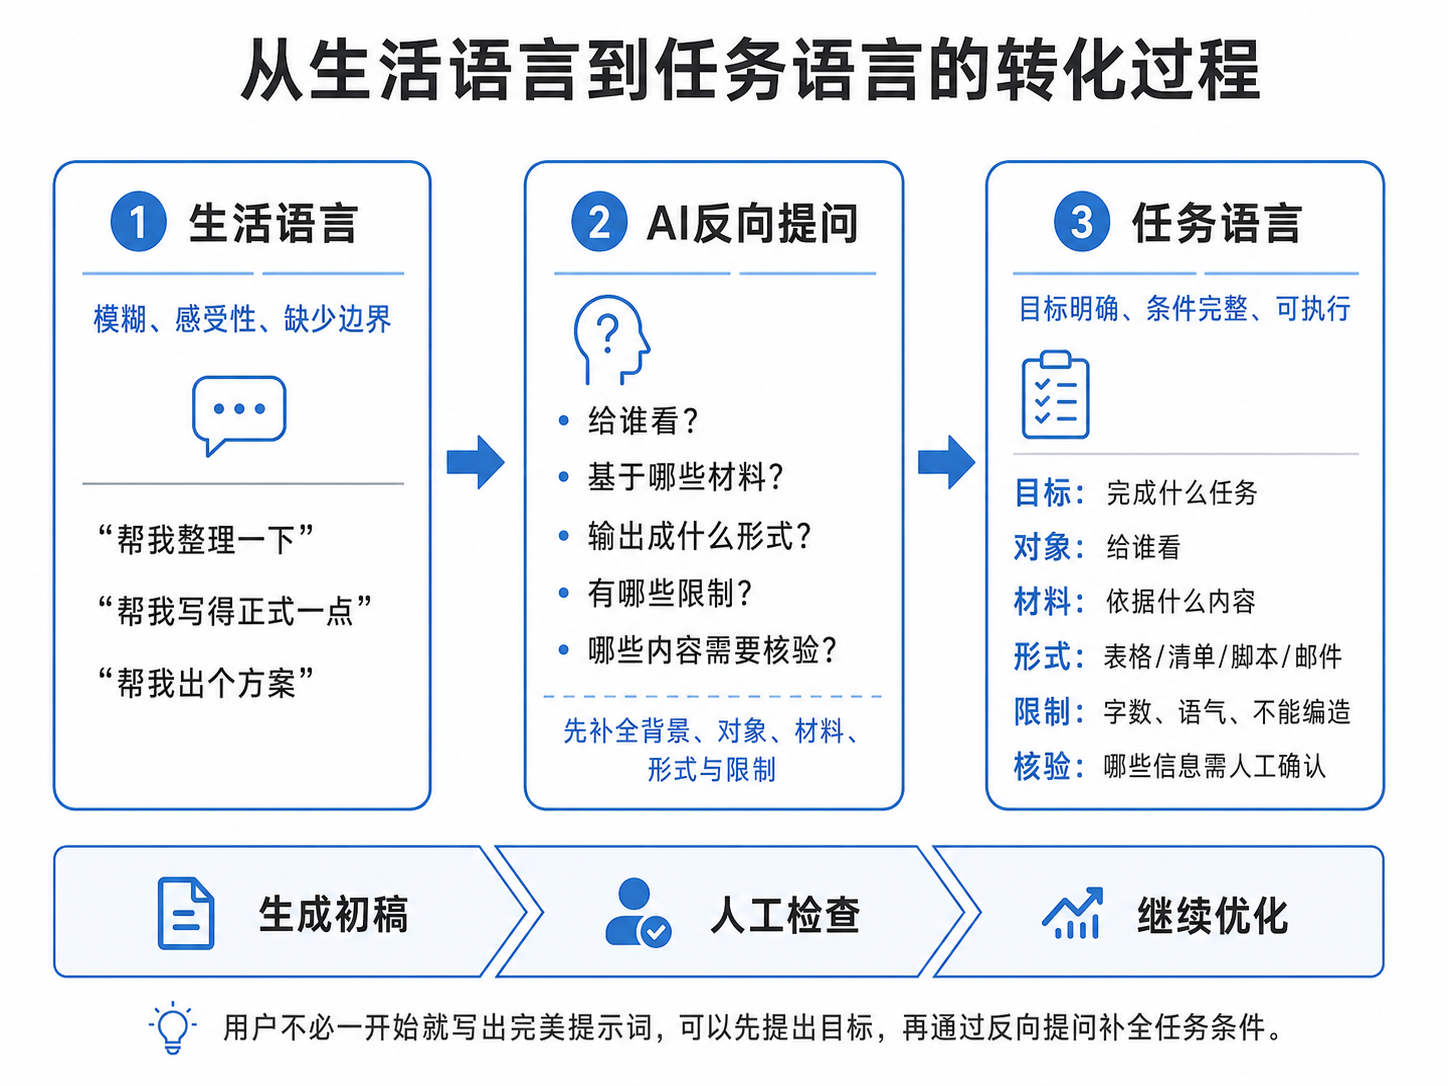
\includegraphics[width=0.88\textwidth]{images_8/ChatGPT Image 2026年5月26日 16_25_33.png}
    \caption{从生活语言到任务语言的转化过程}
    \label{fig:life-to-task-process}
\end{figure}
\FloatBarrier



一些新的 AI 工具已经开始提供提示词生成和提示词优化能力，可以根据任务目标自动补充背景、格式、变量和评价标准。这说明，提示词的使用方式正在从“手写复杂模板”转向“提出目标后由 AI 辅助完善”。

不过，AI 能优化提示词，并不代表用户可以跳过需求拆解。工具只能帮助把指令写得更完整，却不能替人判断真正要解决什么问题、应该提供哪些材料、输出给谁看、哪些内容不能编造、哪些结果需要人工核验。因此，实际使用时，重点不再是记住某个“万能提示词公式”，而是先把目标、材料、格式和限制说清楚，再让 AI 帮助完善指令。

在实际使用中，复杂任务也不宜一次性全部交给 AI 完成。更稳妥的方法，是把大任务拆成几个连续的小步骤。比如制作 AI 短剧，可以先确定主题和故事梗概，再生成角色设定、分镜脚本、画面提示词、配音文案和发布说明；准备会议汇报，可以先整理资料，再提炼观点，接着生成发言提纲，最后改成适合现场表达的口语稿；办理生活事务，可以先梳理材料清单，再生成咨询话术，最后整理注意事项。分步完成的好处是，每一步都可以人工检查和调整，避免 AI 在前一步理解错误的情况下继续生成后续内容。

当一个任务只做一次时，写清楚提示词就可以了；但如果同一类任务会反复出现，就可以把它整理成 Skill。Skill 可以理解为一套可复用的任务说明书，它告诉 AI：什么时候使用这个能力、需要提供什么材料、应该按什么步骤处理、最终输出什么格式，以及哪些内容必须提醒人工确认。

如果后续使用 opencode 这类 Agent 工具，Skill 还可以进一步整理成独立文件或项目规则，让智能体在合适的任务中读取并执行。这样，AI 的使用就不再只是每次临时写一段提示词，而是把常用任务沉淀成可以长期调用的工作流程。

下面以“家乡特产一周内容策划 Skill”为例，完成一次 Skill 构建。

\minorheading{步骤一：选定具体任务}

我要为一个家乡特产设计一周的宣传内容。

可以先打开任意一个 AI 软件官网或者 App，输入下面这句话：

\begin{tcolorbox}[promptbox]
我想为一个家乡特产做一周宣传，但我还没有想清楚具体内容。请你先不要直接写文案，而是先问我 6 个必须确认的问题，帮助我把任务说清楚。
\end{tcolorbox}

这一步的目的不是马上生成结果，而是先让 AI 帮你补全任务条件。围绕“一周宣传内容”这个任务，AI 通常会继续确认几个关键信息：产品是什么、有什么特点、目标人群是谁、准备在哪个平台发布、手里是否已有图片或视频素材、哪些内容不能夸大、哪些信息需要人工确认。把这些问题回答清楚以后，后面的内容计划才会更贴近真实需求。

\begin{figure}[H]
    \centering
    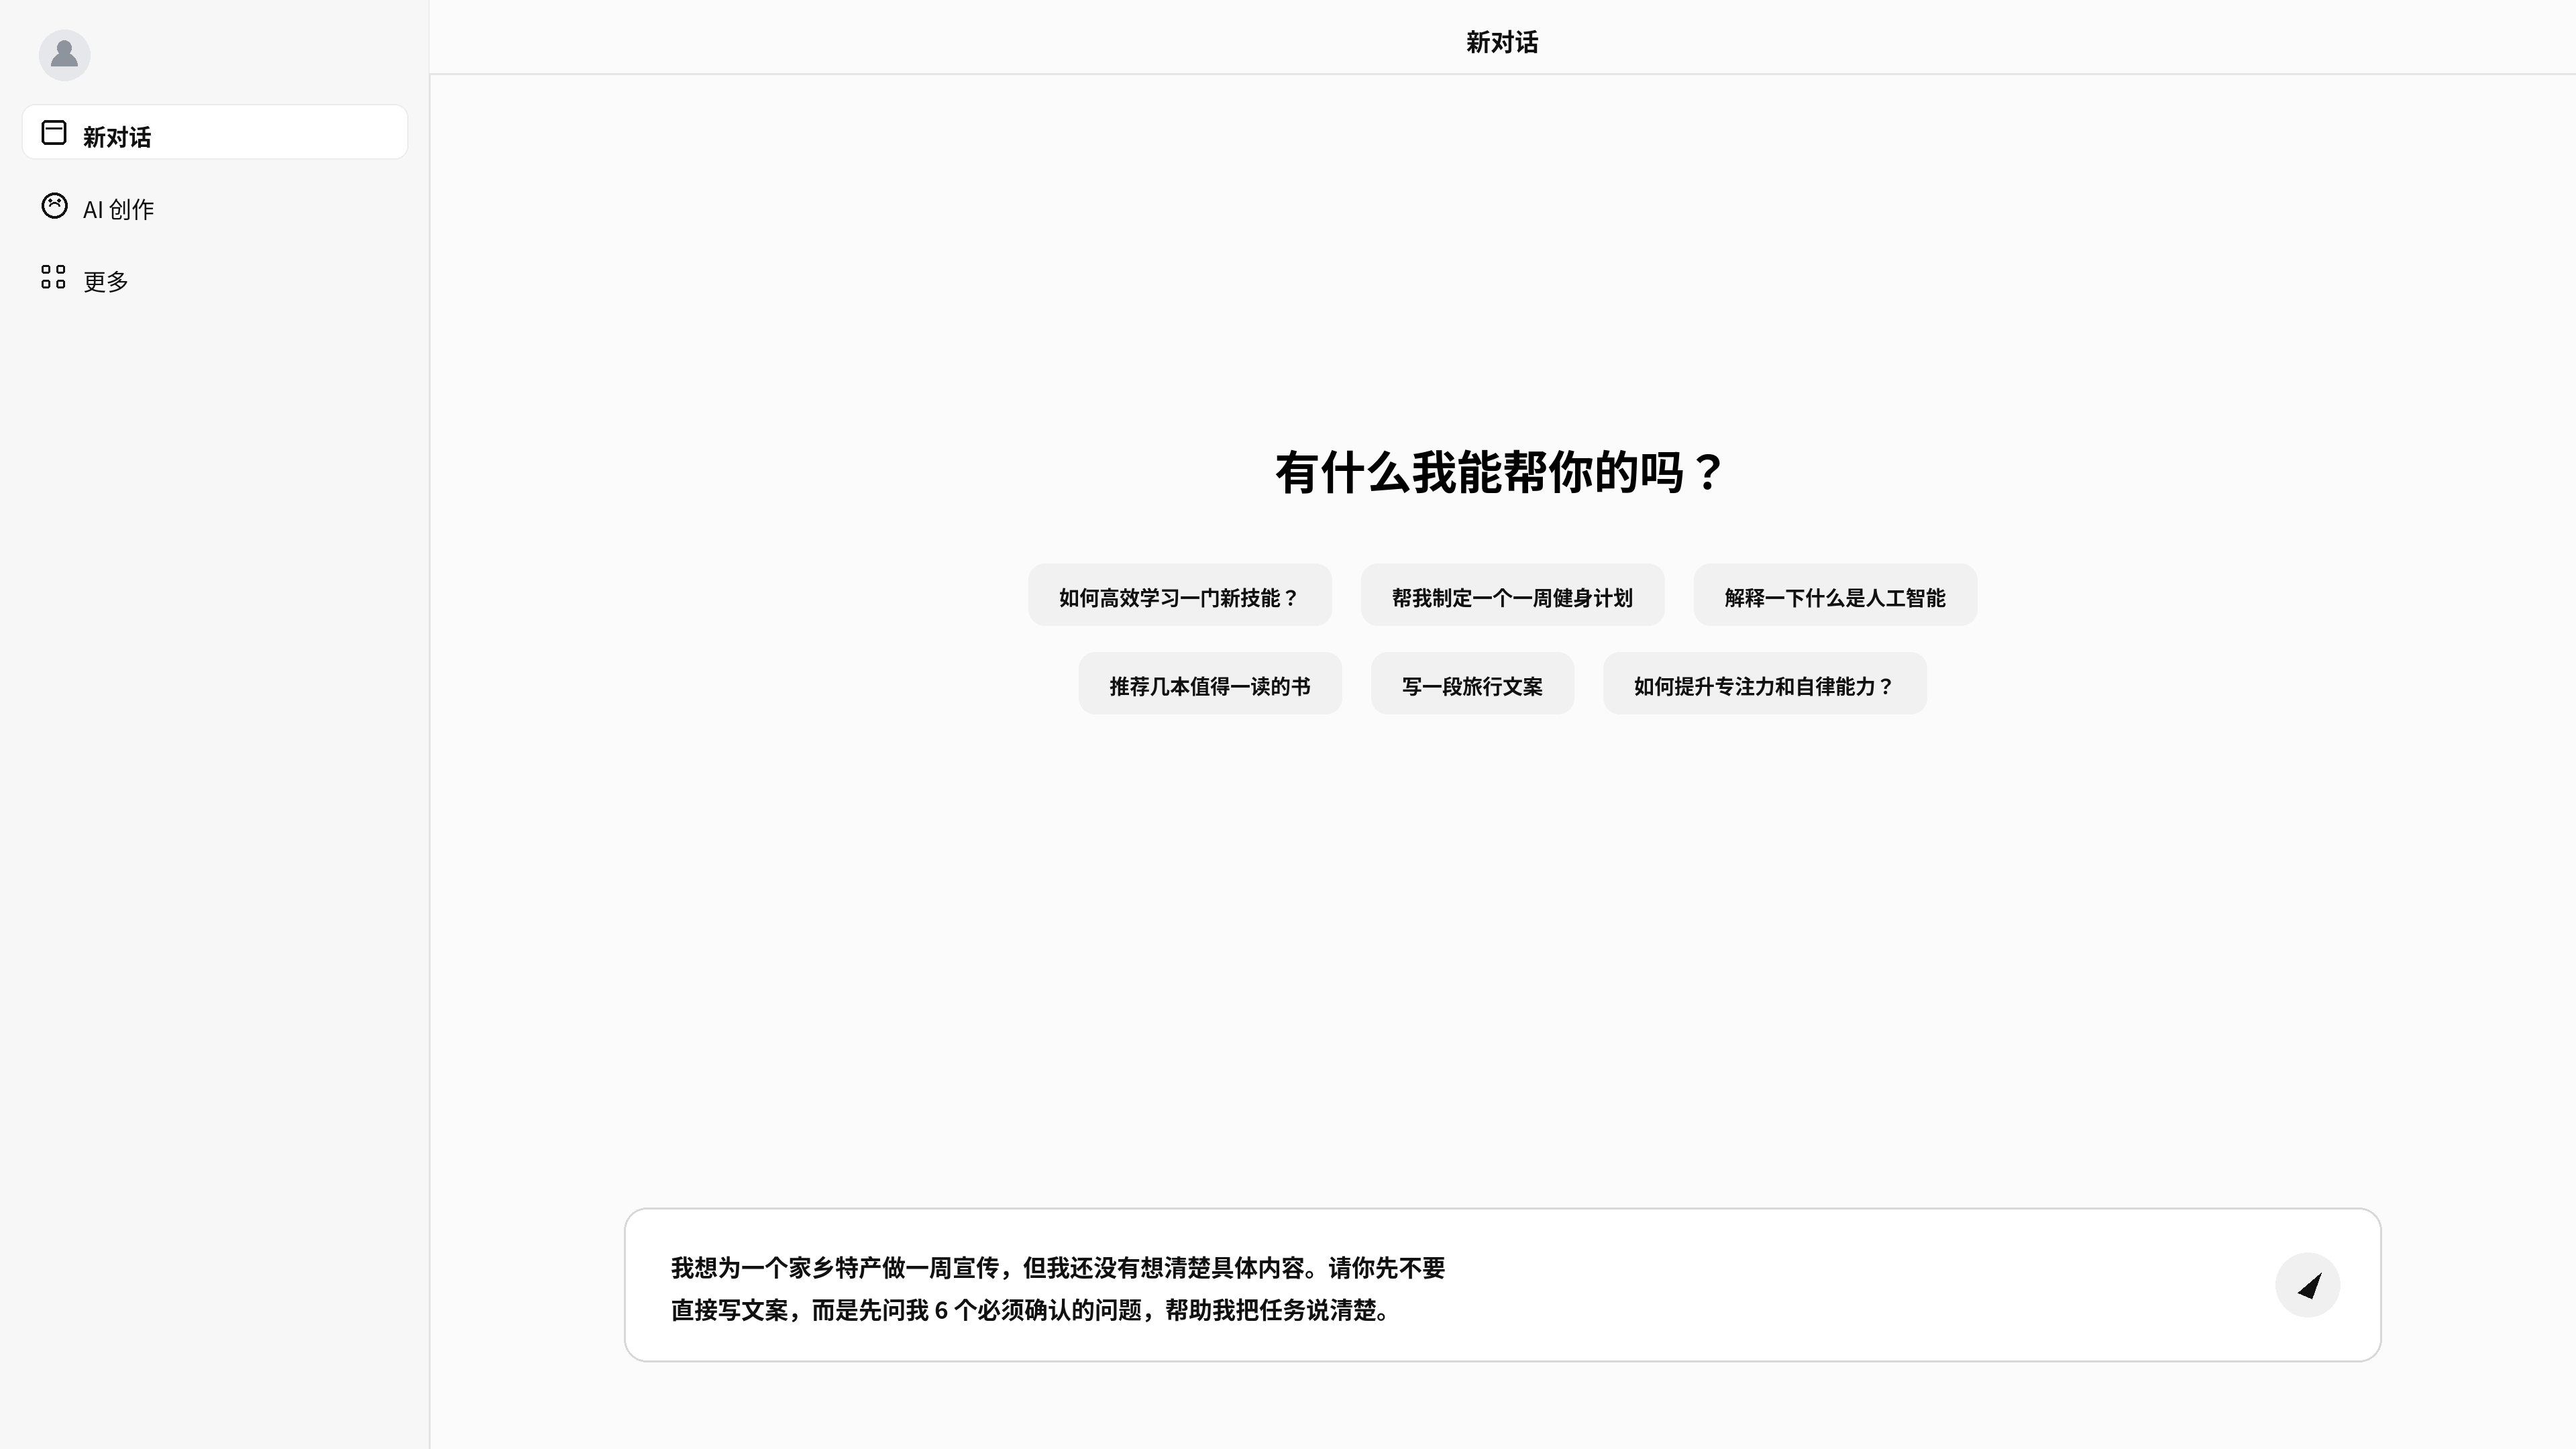
\includegraphics[width=0.88\textwidth]{images_8/步骤1_AI输入界面_4K超高清.png}
    \caption{提出任务目标，让 AI 先反向提问}
    \label{fig:skill-step-question}
\end{figure}
\FloatBarrier

\minorheading{步骤二：补充任务材料}

AI 提出问题后，就可以根据自己的真实情况逐项补充信息。比如，想为家乡特产做一周宣传时，可以这样回答：

\begin{tcolorbox}[promptbox]
产品名称：家乡手工煎饼。

产品特点：薄、脆、有麦香，可以卷菜、卷肉，也可以当零食。

目标人群：年轻上班族、外地游客、想买家乡特产的人。

发布平台：小红书、朋友圈、抖音。

已有素材：有煎饼图片、包装图片、制作过程短视频。

限制条件：不能夸大养生功效，不能编造销量，价格、库存和物流需要人工确认。
\end{tcolorbox}

这样补充以后，AI 获得的就不再是一句模糊的“帮我宣传一下”，而是一组比较完整的任务条件。它知道要宣传什么产品，产品有什么特点，内容写给谁看，准备发到哪些平台，手里有哪些素材，哪些内容不能乱写，哪些信息必须由人确认。

\begin{figure}[H]
    \centering
    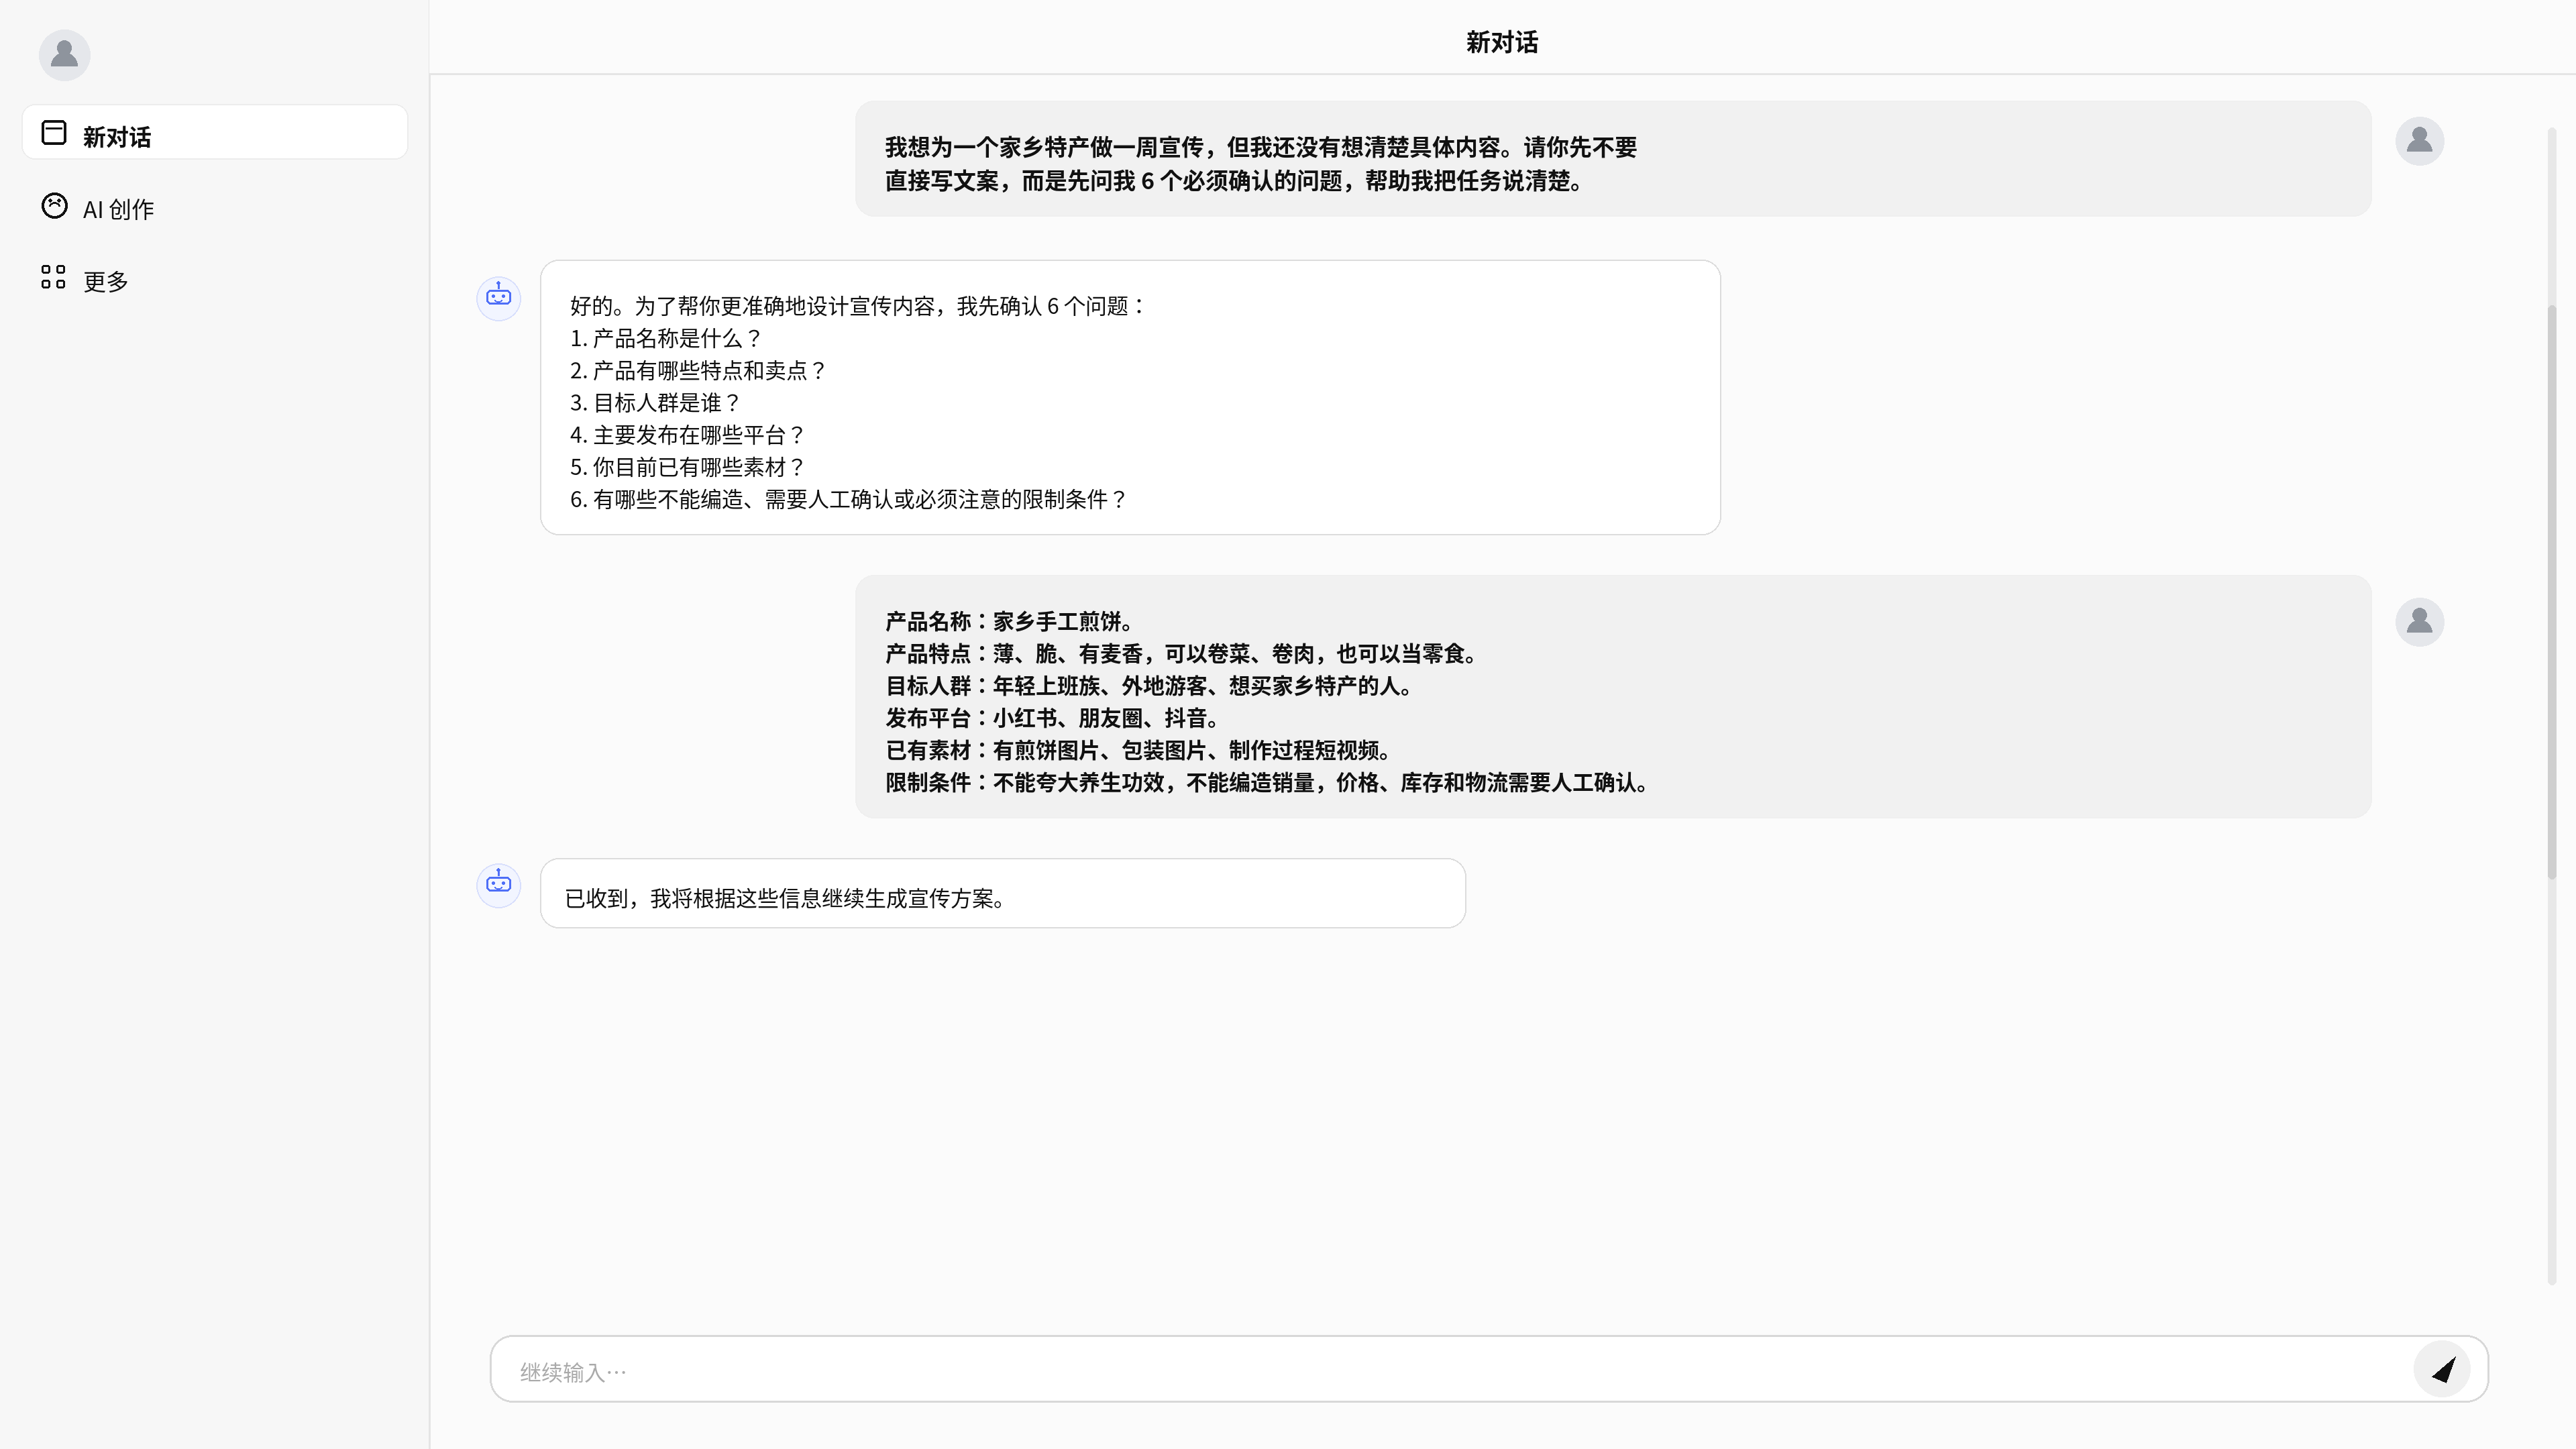
\includegraphics[width=0.88\textwidth]{images_8/步骤2_AI聊天记录界面_4K超高清.png}
    \caption{根据 AI 提问补充任务材料}
    \label{fig:skill-step-material}
\end{figure}
\FloatBarrier

\minorheading{步骤三：生成内容计划}

材料补充完以后，再让 AI 生成第一版结果。可以输入：

\begin{tcolorbox}[promptbox]
请根据我刚才提供的信息，为“家乡手工煎饼”设计一周内容计划。

要求：每天一个不同主题，适合小红书、朋友圈和抖音使用。

请用表格输出，表头包括：日期、内容主题、标题方向、核心文案、短视频脚本方向、素材建议、需要人工核验的信息。

注意：不要编造价格、销量、功效、荣誉和用户评价。
\end{tcolorbox}

这时，AI 生成的结果可能已经比较完整。接下来不能直接照搬，而是检查这份内容计划是否好用。

可以重点看四个问题：

第一，每天的内容是不是重复。

第二，标题是不是适合目标平台。

第三，短视频脚本方向能不能真的拍出来。

第四，有没有把价格、库存、功效、销量等内容标成“需要人工核验”。

如果发现结果太空，可以继续追问：

\begin{tcolorbox}[promptbox]
这些标题有点普通，请改得更适合小红书，但不要夸张，不要像广告。

第 3 天的短视频方向不容易拍，请改成普通手机也能完成的拍法。
\end{tcolorbox}

\begin{figure}[H]
    \centering
    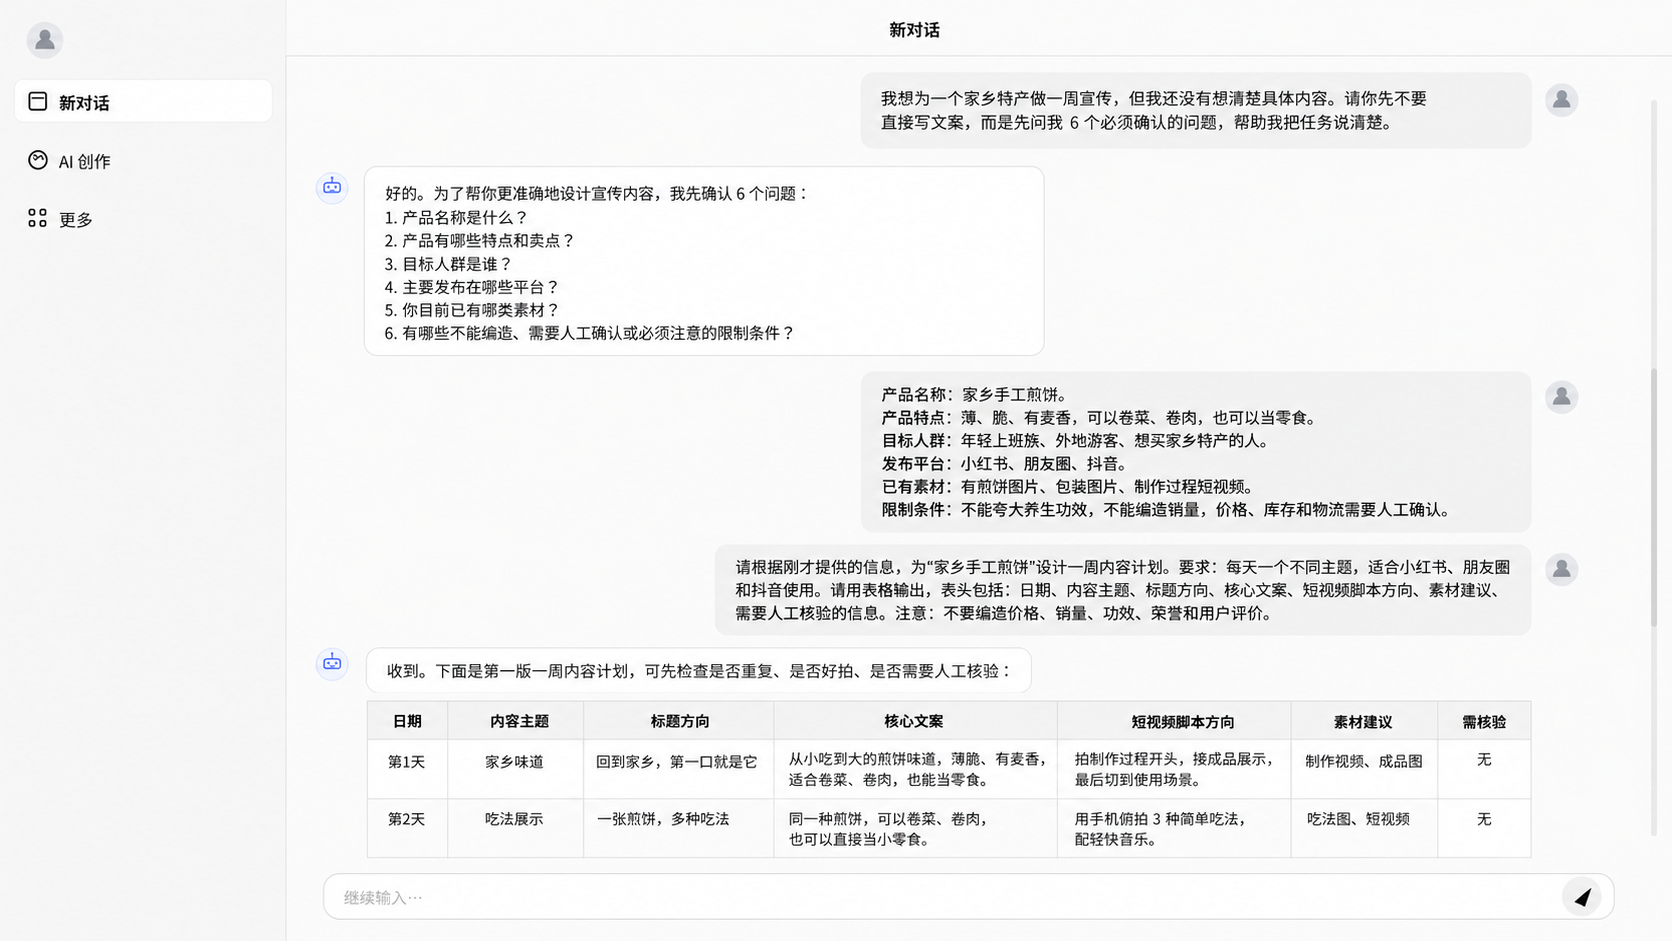
\includegraphics[width=0.88\linewidth]{ChatGPT Image 2026年5月27日 02_12_26.png}
    \caption{生成计划内容}
    \label{fig:placeholder}
\end{figure}

\minorheading{步骤四：沉淀为 Skill}

当这套流程比较好用，就可以把它保存成 Skill。如果不熟悉计算机操作，也不需要一开始就写代码或创建复杂文件夹。最简单的方法是：打开 WPS、备忘录或飞书文档，新建一个文档，标题写成：

\begin{tcolorbox}[promptbox]
家乡特产一周内容策划 Skill
\end{tcolorbox}

然后把下面这份内容复制进去。

\begin{tcolorbox}[skillbox,title=家乡特产一周内容策划 Skill]
\textbf{Skill 名称：} 家乡特产一周内容策划助手

\textbf{适用场景：}

当需要为家乡特产、地方美食、校园文创、非遗产品或轻量经营项目设计一周宣传内容时，使用本 Skill。

\textbf{需要提供的信息：}

产品或主题名称；产品特点；目标人群；发布平台；已有图片、视频或文字资料；推广周期；不能夸大的内容；需要人工确认的信息。

\textbf{执行步骤：}

第一步，先提炼产品或主题的核心卖点，包括产地、口味、使用场景、故事和适合人群。

第二步，判断目标受众关心什么，例如价格、口味、方便程度、送礼价值、地方特色。

第三步，设计一周内容计划，每天一个不同角度，避免重复宣传。

第四步，为每天内容生成标题方向、核心文案、短视频脚本方向和素材建议。

第五步，标出所有需要人工核验的信息。

\textbf{输出格式：}

请用表格输出，表头为：日期、内容主题、标题方向、核心文案、短视频脚本方向、素材建议、需要人工核验的信息。

\textbf{注意事项：}

不要编造价格、库存、销量、荣誉、功效、用户评价和物流承诺。涉及价格、库存、发货时间、功效描述、素材版权和宣传效果的内容，都要标注“需要人工确认”。不要直接替用户发布内容，只提供可修改的策划方案。
\end{tcolorbox}

这一步完成后，就已经拥有了一个最基础的 Skill。它本质上是一份“可反复使用的任务说明书”。以后只要换一个产品，比如“家乡苹果”“地方糕点”“校园文创帆布包”“非遗香包”，都可以继续使用这份 Skill。

需求拆解和指令构建，是后续所有 AI 应用场景的基础。无论是出行规划、学习辅导、生活办事、会议协作，还是职业经营、内容创作和跨文化表达，本质上都需要先把模糊需求变成清晰任务，再让 AI 根据任务要求生成可检查、可修改、可复用的结果。掌握这一方法之后，AI 的使用就不再停留在“想到什么问什么”的临时提问，而会逐渐变成一种有步骤、有标准、能沉淀的智能协作方式。

\subsection{Skill 迭代与能力沉淀}

完成一个 Skill 之后，更重要的事情是让它在以后的任务中持续发挥作用。前面构建的“家乡特产一周内容策划 Skill”，已经把一次临时提问整理成了可复用的任务说明。但真正成熟的 Skill，不只是保存在文档里的一段提示词，而是能够被反复调用、不断修改，并逐渐形成个人 AI 能力库的一部分。

保存 Skill 时，可以先从最简单的方式开始。可以在 WPS、飞书文档、备忘录或网盘中新建一个文件夹，命名为“我的 AI Skill 库”。每一个 Skill 单独保存成一个文档，标题尽量清楚，例如“内容策划 Skill”“短视频脚本 Skill”“客户回复 Skill”“会议纪要 Skill”“发布审查 Skill”。以后遇到类似任务时，不需要重新组织完整提示词，只需要打开对应文档，替换新的主题、材料和限制条件即可。

一个值得长期保存的 Skill，通常有三个特点：第一，这类任务会反复出现；第二，它能明显节省整理和表达的时间；第三，它有相对固定的输出格式和检查标准。比如，随手写一句节日祝福，通常不需要专门保存成 Skill；但整理会议纪要、生成一周内容计划、撰写客户回复、检查发布风险，就很适合沉淀下来。因为这些任务不仅经常出现，而且每次都需要按照一定步骤完成，输出结果也需要保持稳定。

Skill 保存以后，还要在使用中继续修改。比如，“内容策划 Skill”第一次使用时，可能已经能生成一周选题，但标题有些夸张，脚本不方便拍摄，或者风险提示不够明显。这时就可以回到 Skill 文档中补充规则，例如：“标题要自然可信，不使用夸张营销话术”；“短视频脚本应适合普通手机拍摄”；“涉及价格、库存、功效、销量、用户评价和版权素材时，必须标注需要人工确认”。这样，Skill 就会在一次次使用中变得更稳定。

现在一些 AI 平台也开始把提示词生成、提示词优化和结果评估做成工具。比如 OpenAI 的 Prompt Optimizer 可以根据任务目标改进提示词；Anthropic 也在相关文档中强调，智能体应用正在从单纯的 prompt engineering 走向更重视上下文组织、工具说明和持续迭代的 context engineering。这样的趋势说明，AI 使用正在从“写一次提示词”发展为“持续优化任务流程”。实际使用时，不一定要掌握复杂技术，但要形成一个意识：好用的提示词和 Skill 都不是一次写成的，而是在实际任务中不断测试、调整和积累出来的。

当 Skill 越来越多时，还需要学会分类。可以把个人 Skill 库分成几类：“信息整理类”用于整理通知、会议记录、资料和文件；“内容创作类”用于生成选题、脚本、文案和标题；“沟通表达类”用于写邮件、客户回复、求职介绍和会议发言；“检查审查类”用于核对事实、隐私、版权和风险；“复盘总结类”用于记录反馈、总结问题和改进下一步行动。分类的目的不是为了形式整齐，而是为了在真正需要时能够快速找到对应工具。

\begin{figure}[H]
    \centering
    
\includegraphics[width=0.88\textwidth]{images_8/8.2.1.png}
    \caption{个人 AI Skill 库的组织与调用流程}
    \label{fig:skill-library-flow}
\end{figure}
\FloatBarrier

单个 Skill 只能完成一个环节，多个 Skill 组合起来，才能形成完整流程。以前面的“家乡特产一周内容策划 Skill”为例，它主要解决“这一周发什么内容”的问题。如果要完成一次完整推广，还需要先用“资料整理 Skill”提炼产品卖点，再用“内容策划 Skill”生成一周选题，用“短视频脚本 Skill”扩写分镜和口播，用“客户回复 Skill”准备常见问答，用“发布审查 Skill”检查事实、隐私、版权和夸大宣传，最后用“复盘总结 Skill”记录发布效果和改进方向。这样，AI 的使用就从一个个孤立任务，逐渐变成一套可以持续运行的个人工作流。

需要注意的是，Skill 的作用是提高效率和稳定性，而不是替人承担责任。整理资料、生成初稿、制作清单、提出建议，通常可以交给 AI 辅助；但涉及公开发布、填写表单、确认价格、承诺服务、上传资料、发送信息等操作时，必须由人进行最终确认。只有把 Skill 管好、改好、组合好，并始终保留人的判断，AI 才能真正成为长期可靠的学习、工作和生活助手。

\section{出行服务与跨语言沟通}

\subsection{行前准备与行程规划}

出行准备看似是一件小事，但很多麻烦都发生在出门之前。有人去医院复查，到了窗口才发现忘带检查报告；有人去政务大厅办业务，排了半小时队才知道还缺一张复印件；有人去考试，路线查得很清楚，却没有考虑早高峰、安检和找考场时间；也有人去陌生城市参加活动，酒店、会场、交通、天气都分开查了一遍，最后还是手忙脚乱。由此可见，出行不是简单的“从哪里到哪里”，而是一个包含路线、时间、材料、流程和突发情况的综合任务。

现在的 AI 出行辅助，已经不再只是导航工具。过去使用地图，主要是为了知道“从哪里到哪里怎么走”；而现在，AI 可以围绕一次出行做更完整的安排。比如去医院复查，可以让 AI 提醒你提前查看挂号时间、准备证件、估算路上时间；去参加会议，可以让 AI 帮你确认地点、规划出发时间、整理需要携带的材料；周末出去玩，也可以让 AI 结合天气、距离和同行人员，帮你选择更合适的路线和活动。这样一来，AI 解决的就不只是“怎么走”，而是“这次出门怎样安排更顺利”。

出发前使用 AI，可以按照\textbf{“一个目标、三类信息、两项确认”}来整理。

\textbf{一个目标}，就是先说清楚这次出门到底要完成什么事情。比如“去医院复诊”“去参加考试”“去办证”“去面试”“去参加活动”。不同目标，对应的准备重点是不一样的。去医院，重点可能是病历、检查报告、医保卡和挂号时间；去考试，重点是准考证、身份证、入场时间和考场位置；去面试，重点是简历、作品集、着装和公司地址；去办证，重点是材料、照片、预约记录和办公时间。目标说得越清楚，AI 才越容易帮你查漏补缺。

\textbf{三类信息}，可以理解成出门前要想明白的三件事：怎么去、带什么、到了怎么办。
第一类是路线信息，包括从哪里出发、几点要到、坐地铁还是打车、需不需要换乘、下车后还要走多远。第二类是材料信息，包括证件、文件、照片、票据、预约记录、证明材料等。第三类是现场信息，比如办公楼在哪一栋、入口在哪里、去几楼、找哪个窗口、是否需要排队、有没有安检要求、附近能不能停车。这样整理以后，出门就不只是“导航到某地”，而是一份更完整的行动安排。

\textbf{两项确认}，是为了避免“AI 说得很顺，但实际用不了”。第一项是官方确认。AI 可以帮你整理和提醒，但不能替代官方通知。时间、地点、材料、费用、预约、考试规则、医院安排等信息，最后都要回到地图实时信息、医院平台、学校通知、政务平台或活动通知中核对。第二项是备用方案确认。比如堵车怎么办，地铁临时停运怎么办，材料少带了怎么办，手机没电了怎么办。提前让 AI 帮你想一遍这些情况，真正出门时就不容易手忙脚乱。

下面选取医院复诊、考试和政务办事三个常见场景，说明 AI 如何把出门前容易遗漏的事项整理成清单。

如果是去医院复诊，可以这样输入：

\begin{tcolorbox}[promptbox]
明天上午 9 点我要去医院复查，从家里出发，最好提前 20 分钟到。请帮我整理一份出门前准备清单，包括建议出发时间、交通路线、可能需要带的材料、要问医生的问题、路上可能出现的风险和备用方案。不能确定的信息请标注“需要我自己确认”。
\end{tcolorbox}

这类清单可以包括四个部分：一是出发时间和路线安排，例如是否需要预留早高峰、排队和找科室的时间；二是需要携带的材料，例如身份证、医保卡、挂号记录、检查报告、病历本和正在服用的药物清单；三是复诊时想咨询的问题，例如症状是否加重、药物是否需要调整、是否需要复查项目；四是备用方案，例如交通拥堵时是否改乘地铁、找不到科室时如何询问导诊台、预约信息不一致时如何处理。

如果是参加考试，可以换成下面这个提示：

\begin{tcolorbox}[promptbox]
我明天上午要参加考试，9 点开始，考点在某某学校。我从家出发，请帮我整理出行准备清单，包括建议出发时间、交通方案、需要携带的证件和文具、考前注意事项、迟到风险和备用方案。请提醒我哪些信息必须再去准考证或官方通知中核对。
\end{tcolorbox}

这类提示的重点，是让 AI 把“出门”拆成几个可检查的环节。考试场景中，路线只是其中一项，更重要的是准考证、身份证、文具、入场时间、考场位置、安检要求、禁止携带物品和迟到后果。AI 可以帮你列出清单，但最终仍要以准考证和考试官方通知为准。

如果是去政务大厅办事，可以这样输入：

\begin{tcolorbox}[promptbox]
我准备去政务大厅办理业务，但不确定要带什么材料。请帮我整理出门前需要确认的内容，包括办理地点、办公时间、可能需要的证件、复印件、照片、线上预约、咨询电话和现场排队风险。不能确定的信息请标注“需要官方确认”。
\end{tcolorbox}

这时，AI 的作用是提前形成一份“办事检查表”。它可以提醒我们确认：是否需要原件和复印件，是否要提前预约，是否必须本人到场，是否需要照片，能不能线上办理，是否有午休时间，到现场后是否需要取号排队。

这些问题看似琐碎，却往往决定一次出门能不能顺利完成。很多办事失败，并不是因为找不到地方，而是因为材料、时间或流程没有提前确认。

前面已经学习过，反复出现的任务可以整理成 Skill。接下来，我们就以更常见的\textbf{“出门旅行”}为例，看看如何把目的地、交通、住宿、预算、天气、预约、行李和备用方案等内容，整理成一个可以反复使用的\textbf{“出门旅行计划 Skill”}。这样以后再做旅行计划时，就不必每次都从零开始问 AI，而是可以让 AI 按照固定流程生成更稳定、更实用的结果。

\minorheading{旅行 Skill：固化行程流程}

制作这个 Skill 时，可以先打开 WPS、飞书文档、备忘录或手机便签，新建一个文档，标题写成：

\begin{tcolorbox}[promptbox]
出门旅行计划 Skill
\end{tcolorbox}

然后把下面这段内容保存进去：

\begin{tcolorbox}[skillbox,title=出门旅行计划 Skill]
你是“出门旅行计划助手”。我会告诉你旅行目的地、出发地、旅行时间、同行人员、预算、兴趣偏好和限制条件。请你帮我整理一份适合普通人执行的旅行计划。

请按照以下步骤完成：

第一步，先概括本次旅行目标，包括去哪里、玩几天、和谁去、主要想体验什么。

第二步，整理出发前需要确认的信息，包括交通方式、住宿位置、天气、门票预约、开放时间、身份证件、行李物品和预算。

第三步，设计每日行程安排。每天的安排要包括上午、下午、晚上三个时间段，并说明每个地点之间的大致衔接方式。行程不要排得太满，要给吃饭、休息、排队和临时调整留出时间。

第四步，整理旅行准备清单，包括证件、衣物、充电设备、常用药品、雨具、防晒用品、现金或支付方式、必要票据等。

第五步，给出备用方案。比如天气不好怎么办、景点没预约上怎么办、同行人走累了怎么办、交通延误怎么办。

第六步，标出所有需要人工确认的信息。凡是涉及车票、酒店、门票、开放时间、价格、天气、交通变化和安全提醒的内容，都必须标注“需要确认”，不能自行编造。

请用表格和清单结合的方式输出，语言要清楚、实用，不要写成广告式旅游攻略。
\end{tcolorbox}

保存好\textbf{“出门旅行计划 Skill”}以后，每次旅行前都可以再次调用它。操作时，先打开一个支持文档上传或长文本输入的 AI 工具，把自己保存的 Skill 文档上传给 AI，或者直接复制到对话框中，作为参考材料提供给 AI。

接着，再补充这一次旅行的真实信息，让 AI 按照 Skill 文档里的步骤生成旅行计划。这个过程的核心是：先让 AI 理解“工作规则”，再让它处理“这一次的具体任务”。这样生成出来的计划，就不会完全依赖 AI 临时发挥，而是会沿着我们提前设计好的流程进行。

例如，上传或提供\textbf{“出门旅行计划 Skill”}文档后，可以继续输入：

\begin{tcolorbox}[promptbox]
我已经提供了“出门旅行计划 Skill”文档。请你先阅读并理解里面的流程，然后按照这个 Skill 的步骤，帮我规划这次旅行。

本次旅行信息如下：

目的地：青岛

出行时间：7 月 10 日到 7 月 13 日

同行人员：两名成年人

预算：中等

偏好：海边、城市散步、本地小吃，不想行程太赶

交通方式：高铁往返

请先检查我提供的信息是否完整，如果还缺少关键信息，请先提问；如果信息已经足够，请按照 Skill 文档生成旅行计划。
\end{tcolorbox}

\begin{figure}[H]
    \centering
    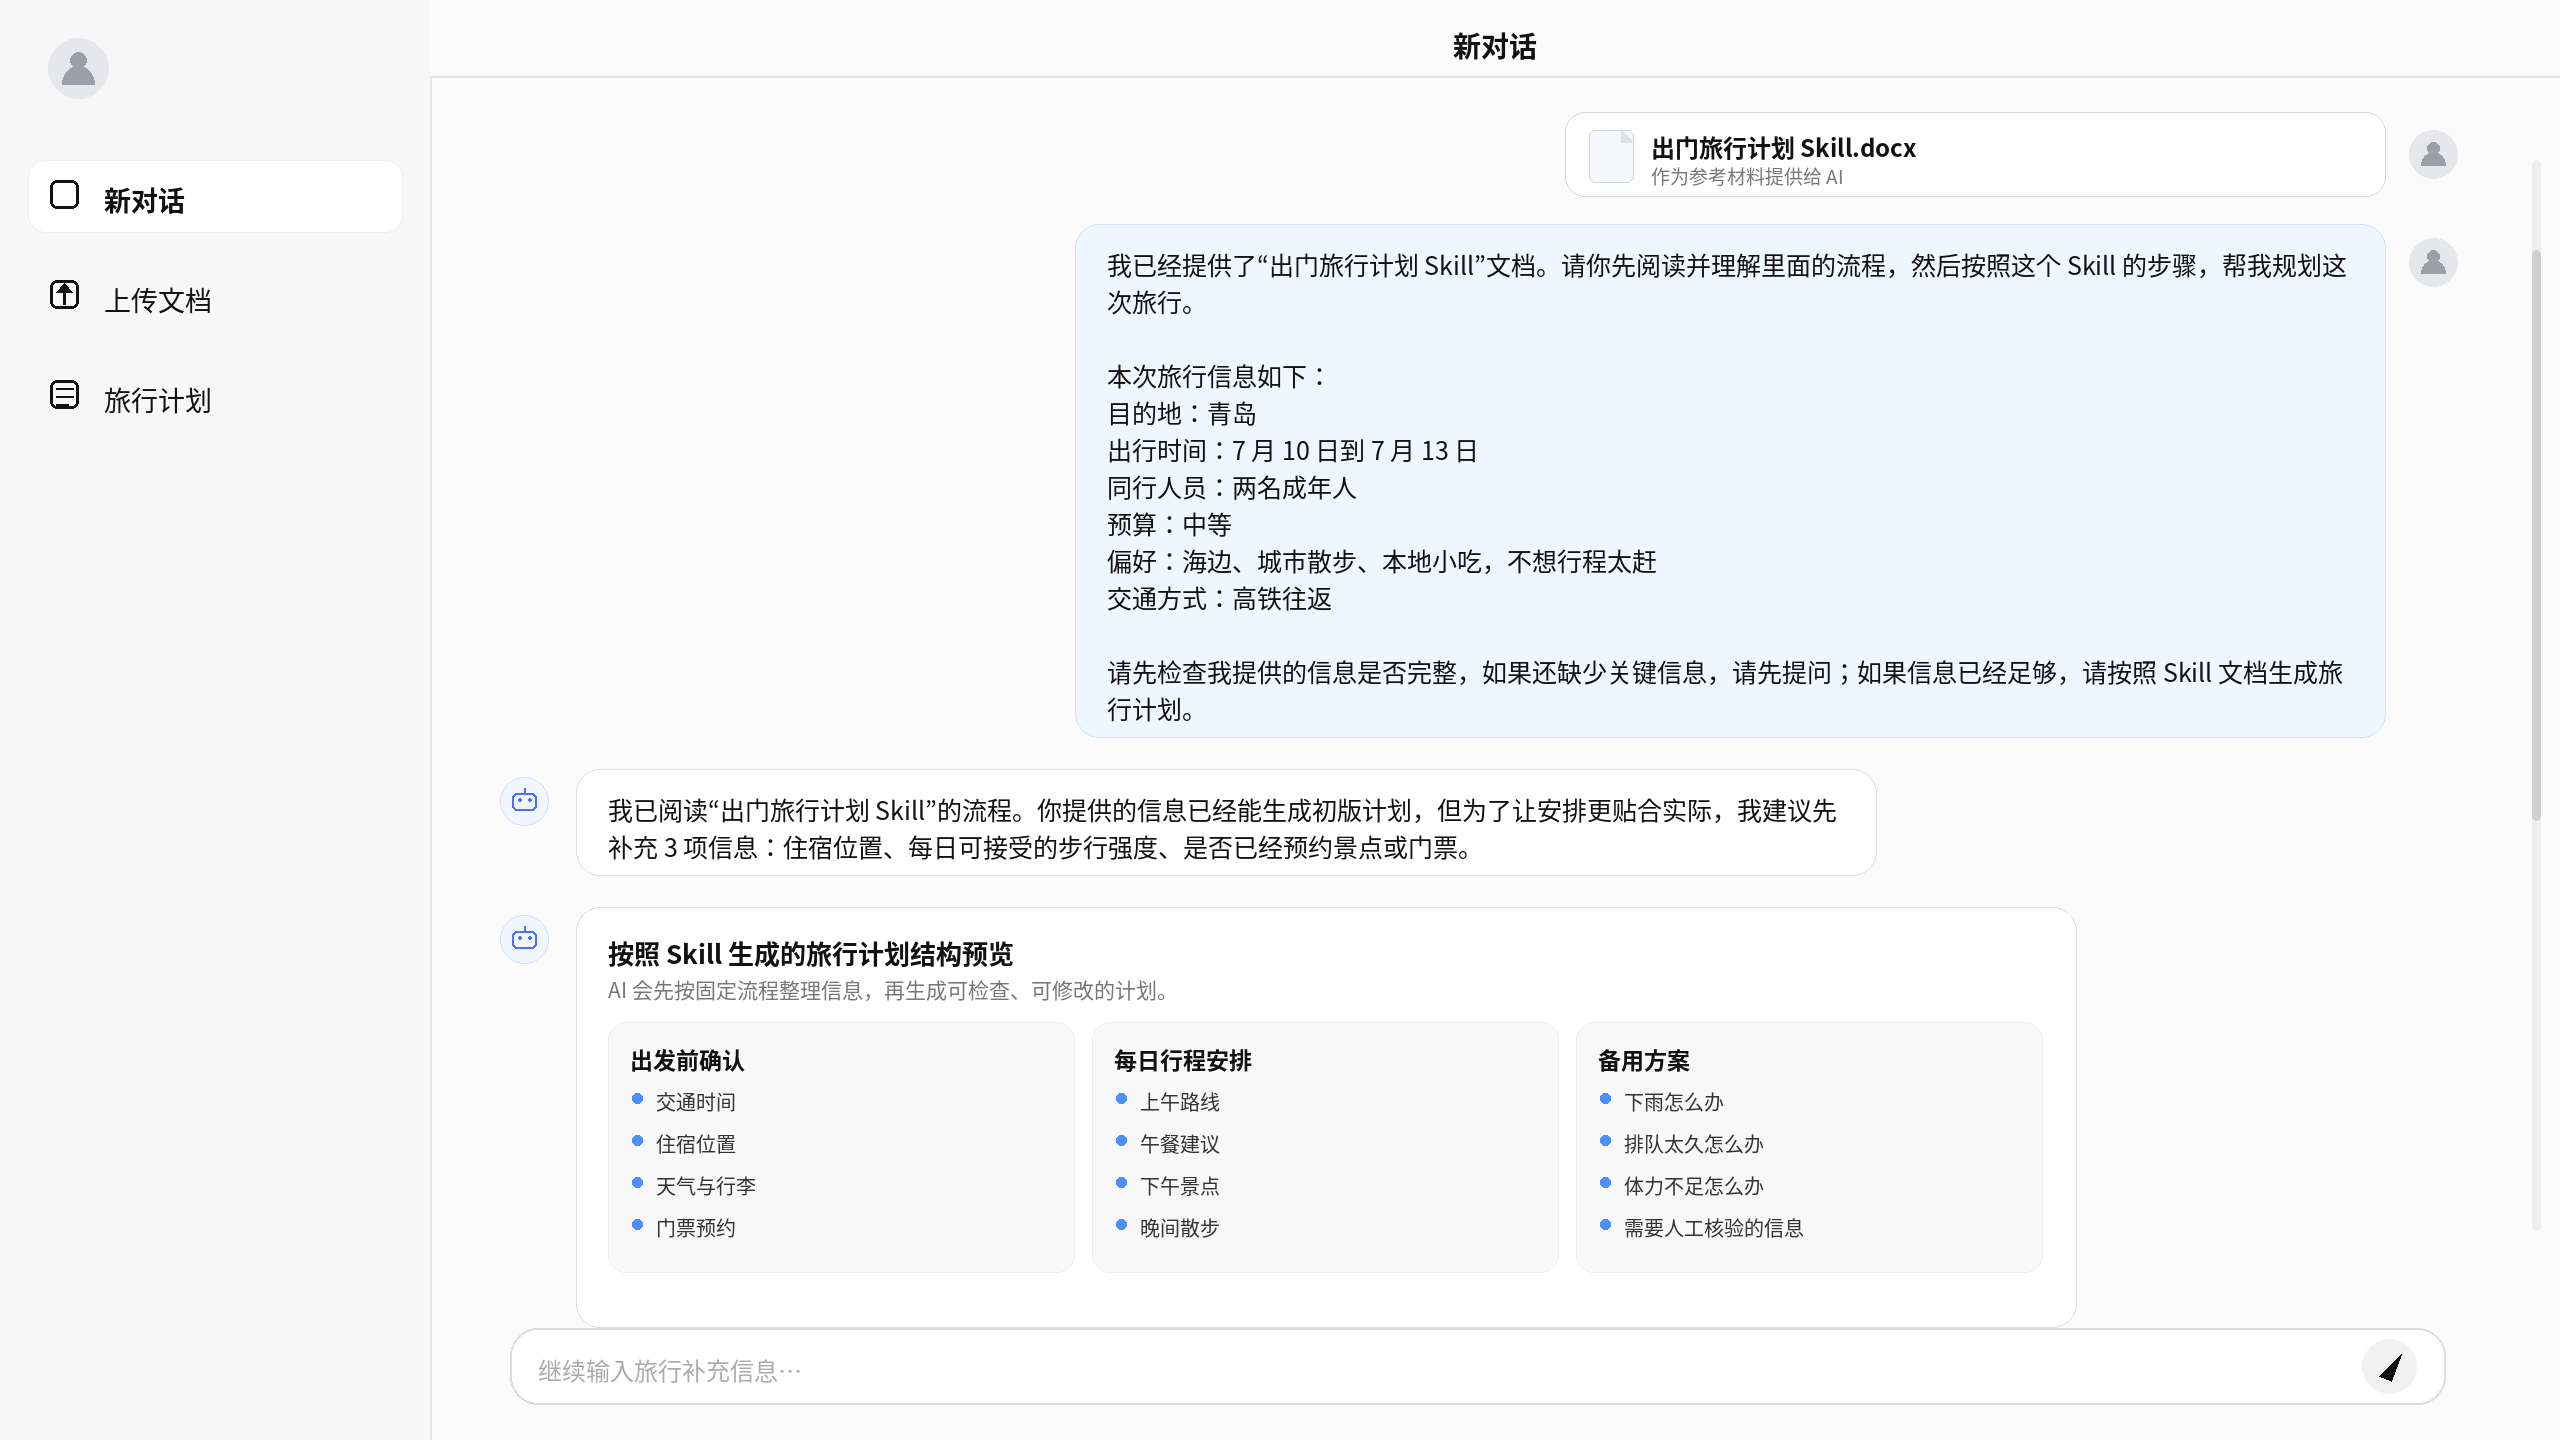
\includegraphics[width=0.88\textwidth]{images_8/出门旅行计划Skill_调用示例_AI界面_2K高清版.png}
    \caption{调用出门旅行计划 Skill 生成行程规划示例}
    \label{fig:travel-skill-call}
\end{figure}
\FloatBarrier




如果是出国旅游，也可以把一些国外平台的 AI 行程规划功能作为辅助工具。例如，Google 在 AI Mode 中加入了 Canvas 旅行规划功能。使用时，只需要描述目的地、旅行时间、预算和偏好，系统就可以生成一份可继续编辑的行程草稿。它不是简单写一段旅游攻略，而是把航班、酒店、地图照片、用户评论和网页资料整合到同一个行程工作区里，帮助你比较住宿、餐厅、活动和路线安排；如果后面想调整计划，也可以继续追问，让系统根据新的需求修改行程。这样，出国旅行时就不必在搜索页面、地图、酒店网站和点评信息之间反复切换，而是可以把它当作一个可持续修改的旅行规划板来使用。

\subsection{在途沟通与即时协同}

出行计划解决的是“出发前怎么安排”，而真正走到路上之后，AI 还可以继续发挥作用。很多时候，旅途中最让人卡住的，并不是目的地没有选好，而是现场突然出现的小问题：看不懂一张菜单，不知道售票机哪个按钮是确认付款，酒店自助入住说明太长，景区公告临时变更，药店标签看不明白，或者餐厅预约需要和店员沟通。尤其是在国外旅行时，这些问题会更加明显，因为语言、规则和操作方式都可能和自己熟悉的环境不同。

这时，AI 的角色就从“行前规划助手”变成了“现场沟通助手”。它不再只是安排路线和行程，而是帮助我们看懂现场信息、生成沟通话术、拆解操作步骤，并提醒哪些内容需要向工作人员确认。例如，手机里的翻译工具已经可以通过摄像头识别菜单、标识牌和说明文字；一些翻译应用也支持实时对话、图片翻译和离线语言包，适合在旅行中处理菜单、街道标识和简单交流问题。

\minorheading{菜单点餐：翻译菜名，判断食材}

在境外餐厅点餐时，菜单往往不是简单的文字翻译问题。许多菜名带有地方特色、烹饪习惯或文化背景，即使被翻译成中文，也未必能让人准确判断它的主要食材、制作方式、口味特点以及是否包含忌口成分。因此，使用 AI 处理菜单时，不宜只停留在“翻译菜名”，而应进一步让 AI 帮助解释菜品内容，并标出需要向服务员确认的信息。

可以这样输入：

\begin{tcolorbox}[promptbox]
我在国外餐厅，请根据我上传的菜单图片，用中文解释每道菜大概是什么。请说明主要食材、烹饪方式、口味可能偏甜/偏辣/偏酸/偏咸，并标出可能含有酒精、海鲜、坚果、牛奶、鸡蛋或生食的菜品。不能确定的地方，请标注“需要向服务员确认”。
\end{tcolorbox}

通过这样的提问，AI 给出的结果就不只是菜单译文，而是一份更接近“点餐辅助说明”的内容。它可以帮助判断某道菜属于主食、汤品、甜点、冷盘还是炸物，也可以提醒某些酱汁、汤底、甜品或腌制食品中可能含有酒精、牛奶、坚果、海鲜等成分。对于有过敏、忌口、宗教饮食或儿童饮食需求的人来说，这类提醒尤其重要。

不过，AI 对食材和过敏原的判断只能作为初步参考，不能代替餐厅确认。菜单图片不清晰、菜名缩写、地方方言、特殊烹饪方式和隐含配料，都可能影响识别和翻译结果。涉及花生、坚果、海鲜、牛奶、鸡蛋、生食、酒精等重要信息时，应当向服务员再次确认。

现场点餐时，还可以让 AI 生成简短、礼貌、便于直接使用的外语表达。例如：

\begin{tcolorbox}[promptbox]
请帮我生成一句英文，用来询问服务员：这道菜是否含有花生？如果含有花生，请推荐一道不含花生的菜。语气礼貌，句子简单，适合现场直接说。
\end{tcolorbox}

AI 可能生成如下表达：

\begin{tcolorbox}[promptbox]
Excuse me, does this dish contain peanuts? If it does, could you recommend a dish without peanuts?
\end{tcolorbox}

点餐类表达不需要复杂，关键是把核心信息说清楚。一般可以按照“想点什么、不能吃什么、需要确认什么”三个部分来组织。也可以提前让 AI 准备几类常用句子：

\begin{tcolorbox}[promptbox]
我不吃生食，请问这道菜是全熟的吗？

我不太能吃辣，请问这道菜可以做成不辣的吗？

我对海鲜过敏，请问这道菜里有没有虾、蟹或鱼露？

我想点一份适合孩子吃的菜，请问哪一道比较清淡？
\end{tcolorbox}

在餐厅场景中，AI 的作用是帮助看懂菜单、理解菜品、准备问句，并降低现场沟通压力；但最终能否食用、是否含有过敏原、是否符合个人饮食要求，仍然需要以餐厅工作人员的确认结果为准。

\minorheading{现场公告：读懂文字，明确行动}

旅行中还有很多信息不是菜单，而是提示牌、交通公告、景区规则、酒店说明、药店标签、商场指示和安全提醒。这类文字往往很短，但影响很大。比如车站屏幕提示某列车换站台，景区入口写着今日部分区域关闭，酒店门口贴着自助入住说明，药品包装上写着服用方式。如果只是逐字翻译，你可能仍然不知道下一步该做什么。

这类场景中，可以让 AI 不只翻译文字，还要解释“这条信息对我有什么影响”。例如，在车站看到公告时，可以输入：

\begin{tcolorbox}[promptbox]
我在车站，请根据我上传的公告图片，帮我判断这条通知和我有什么关系。请用中文说明：它在提醒什么，我是否需要换站台、改路线或重新确认车次，哪些信息必须向工作人员确认。
\end{tcolorbox}

如果是在景区看到提示牌，可以输入：

\begin{tcolorbox}[promptbox]
请根据我上传的景区提示牌，帮我说明这里是否可以进入、是否需要预约、是否有时间限制、是否有安全注意事项。不能确定的地方请标注“需要向工作人员确认”。
\end{tcolorbox}

如果是在酒店自助入住区看到说明，可以输入：

\begin{tcolorbox}[promptbox]
请根据我上传的酒店自助入住说明，帮我整理操作步骤。请告诉我先做什么、后做什么，需要准备哪些信息。涉及护照、信用卡、押金、房间号和验证码的地方，请提醒我自己确认，不要替我判断。
\end{tcolorbox}

这里体现的是 AI 的“现场理解”能力。它不只是把外语变成中文，而是帮助你把外文说明转换成行动步骤：先去哪儿、按什么按钮、准备什么材料、哪些地方要停下来确认。对于旅行者来说，这比单纯翻译更有实用价值。

不过，现场公告和规则具有很强的时效性。车站信息可能几分钟后更新，景区规则可能因为天气和人流临时变化，酒店入住说明也可能因房型、订单和平台不同而不同。因此，AI 可以帮助理解，但不能替代现场工作人员或官方平台的确认。

\minorheading{自助设备：识别界面，谨慎操作}

国外旅行中，自助设备是很常见的难点。自动售票机、自助点餐机、自动贩卖机、地铁充值机、行李寄存柜、投币洗衣机，看起来只是几个按钮，但如果语言不熟，很容易不知道哪个是购买、哪个是取消、哪个是确认付款、哪个是返回上一步。

遇到这类问题时，不要让 AI 直接替自己决定“应该按哪个按钮”。更稳妥的做法，是让 AI 先解释界面，再整理可能的操作步骤。比如面对自动售票机，可以输入：

\begin{tcolorbox}[promptbox]
我面前是一台自助售票机，请根据我上传的屏幕图片，帮我解释每个按钮大概是什么意思，并整理一个安全的操作顺序。不要替我决定购买哪张票。涉及目的地、时间、金额、支付和退款的地方，请标注“需要我自己确认”。
\end{tcolorbox}

AI 能帮助你做到几个层次：先识别界面文字，例如“选择语言”“单程票”“往返票”“确认”“取消”“付款”；再解释按钮功能，例如哪个是继续、哪个是返回、哪个会进入支付；最后整理操作顺序，例如先选择语言，再选择目的地，再选择票种和数量，最后核对金额并付款。

如果是自动贩卖机或自助点餐机，可以这样输入：

\begin{tcolorbox}[promptbox]
请根据我上传的机器界面，帮我说明如何选择商品、如何确认数量、如何付款、如何取消操作。请特别提醒哪些按钮可能是确认付款或取消订单。
\end{tcolorbox}

如果是行李寄存柜，可以这样输入：

\begin{tcolorbox}[promptbox]
我在使用行李寄存柜，请根据屏幕图片帮我解释操作步骤。请提醒我哪些地方涉及付款、取件密码、柜门编号和超时费用，不能确定的地方标注“需要现场确认”。
\end{tcolorbox}

这类场景中，AI 能使用到的程度是“辅助理解界面和步骤”，而不是“替用户完成操作”。最终选择商品、票种、数量、金额、支付方式，都必须由自己确认。尤其是涉及付款、退款、押金、密码、取件码和身份信息时，不要把完整敏感信息上传给 AI，也不要在没有核对清楚的情况下直接点击确认。

\minorheading{预约核对：组织表达，核对凭证}

旅行中经常需要预约餐厅、修改时间、说明迟到、确认订单。很多人不怕吃饭，怕的是打电话、发消息或到店解释不清楚。AI 在这里的价值，是把中文想法整理成清楚、礼貌、适合现场使用的外语表达。

现在一些平台已经开始把 AI 用到预订环节。Google 在 AI Mode 中推出过餐厅预约相关的 agentic 功能，你可以描述人数、时间、地点和菜系偏好，系统会搜索多个预订平台，展示可订选项，并引导到对应页面完成最终预订。Booking.com 也推出了 AI Trip Planner、AI Voice Support、Smart Messenger、Auto-Reply 和 AI Trip Support 等功能，用于旅行规划、住宿沟通和行程支持。

实际使用中，可以先让 AI 生成预约表达。例如：

\begin{tcolorbox}[promptbox]
请帮我写一段英文餐厅预约信息。内容是：我想预约今晚 7 点，两个人，尽量靠窗，其中一位不吃海鲜。如果不能安排靠窗，也可以接受普通座位。语气礼貌、简短。
\end{tcolorbox}

AI 可以帮助生成一段适合发送给餐厅或平台客服的内容。这里的关键是信息要完整：预约时间、人数、座位偏好、忌口要求、是否接受替代方案。这样的表达比临时翻译一句“我要订桌”更有用。

如果已经预约，但到店后前台没有查到记录，可以这样输入：

\begin{tcolorbox}[promptbox]
我预订了今晚 7 点的餐厅，但前台没有查到记录。请帮我整理一段英文说明，包含我的姓名、预约时间、人数、预订平台和订单号，请对方帮忙核对。语气礼貌，不要带责备情绪。
\end{tcolorbox}

AI 生成的表达可以帮助你避免情绪化沟通，把问题说清楚：我已经预订、预约时间是什么、通过哪个平台订的、订单号是什么、希望工作人员帮忙核对。真正沟通时，你仍然要打开订单页面、邮件、短信、平台记录或付款凭证。涉及退款、取消费、迟到保留时间、座位安排和消费规则时，必须以平台和商家答复为准。

\minorheading{健康沟通：辅助表达，确认专业意见}

国外旅行时，如果出现喉咙痛、鼻塞、胃不舒服、轻微擦伤等情况，很多人会去药店买非处方药。但药品说明、成分、剂量和禁忌往往都是外文，容易看不懂。AI 可以帮助整理表达，让药师更容易理解情况。

例如，可以输入：

\begin{tcolorbox}[promptbox]
请帮我生成一段英文：我有点喉咙痛和鼻塞，没有发烧。请问有没有非处方药可以缓解？我对青霉素过敏。请提醒我哪些内容必须向药师确认。
\end{tcolorbox}

如果看到药品包装，可以输入：

\begin{tcolorbox}[promptbox]
请根据我上传的药品包装图片，帮我翻译主要用途、服用方式、注意事项和可能的禁忌。不能确定的内容请标注“必须向药师确认”。
\end{tcolorbox}

这里必须特别强调：AI 只能辅助翻译和表达，不能替代医生或药师。药品剂量、过敏风险、禁忌症、孕妇儿童用药、慢性病用药、是否需要就医，都必须向专业人员确认。尤其是症状严重、持续发烧、胸痛、呼吸困难、严重过敏、外伤出血等情况，应优先联系当地急救或医疗机构。

\subsection{应急求助与流程指引}

旅行中最让人慌张的，往往不是计划之外多走了几步路，而是突然遇到自己无法立刻判断的情况：护照找不到了，钱包被偷了，航班延误导致后续行程接不上，酒店说查不到订单，身体突然不舒服，手机快没电却还要找路，甚至在陌生环境中遇到纠纷或安全风险。遇到这些问题时，很多人的第一反应是着急解释，但越着急越容易说不清楚。AI 在这一小节中的作用，不是替你解决所有突发事件，而是在突发情况下把混乱信息整理成清楚事实、可执行步骤和适合求助的表达。

突发情况首先要分清轻重。一般来说，可以分成四类：第一类是安全类，比如迷路、深夜打不到车、遇到可疑人员、财物被盗；第二类是证件和订单类，比如护照遗失、车票或酒店订单出问题、行李丢失；第三类是健康类，比如发烧、过敏、摔伤、身体不适；第四类是行程变更类，比如航班取消、高铁延误、景点临时关闭、天气突然变化。不同问题的处理方式不同，但第一步都一样：先确认人身安全，再整理事实，最后联系合适的渠道。

\minorheading{事实整理：先说清发生了什么}
遇到突发情况时，可以先把 AI 当作“信息整理助手”，不要一上来就让它判断责任，也不要只问一句“我该怎么办”。更稳妥的做法，是先把当前情况说清楚，再让 AI 帮你整理成可以拿去求助的说明。

第一步，先用最简单的话描述发生了什么。比如：

\begin{tcolorbox}[promptbox]
我现在在国外旅行，发现护照找不到了。我有点着急，请先帮我判断还需要补充哪些关键信息。
\end{tcolorbox}

这一步不是为了马上得到答案，而是先让 AI 帮你把问题拆开。它通常会提醒你补充几个关键信息：什么时候发现护照不见的，最后一次看到护照在哪里，之后去过哪些地方，手里有没有护照照片或复印件，是否已经联系酒店、车站、机场、警方或现场工作人员，后续航班和酒店是否会受到影响。

第二步，把自己已经知道的信息补充进去。比如：

\begin{tcolorbox}[promptbox]
我是今天晚上 8 点发现护照不见的。

最后一次确认护照在身边，是下午 2 点在酒店前台办理入住时。

之后我去了景区、餐厅和便利店。

我手机里有护照首页照片和签证页照片，但没有纸质复印件。

我还没有报警，也还没有联系使领馆。

明天下午有返程航班，现在担心会影响登机和出境。

请帮我把这些信息整理成一段求助说明，并列出我下一步需要联系哪些对象。
\end{tcolorbox}

第三步，让 AI 把这些信息整理成清楚的求助说明。可以继续输入：

\begin{tcolorbox}[promptbox]
请把上面的信息整理成“事实经过—当前困难—需要帮助—下一步确认事项”的格式。

语言要清楚、简短，适合给酒店前台、警方、机场工作人员或使领馆工作人员说明情况。

不要替我判断官方流程，涉及报警、补办证件、出入境和航班的问题，请标注“需要向官方渠道确认”。
\end{tcolorbox}

AI 整理后的内容可以是：

\begin{tcolorbox}[promptbox]
我在旅行途中发现护照遗失。今天下午 2 点，我在酒店前台办理入住时最后一次确认护照在身边；之后去过景区、餐厅和便利店。晚上 8 点左右，我发现护照原件暂时找不到。目前手机里保存有护照首页和签证页照片，但没有纸质复印件。我尚未报警，也尚未联系中国驻当地使领馆。由于明天下午有返程航班，我需要确认是否应先联系当地警方、酒店或使领馆，以及证件遗失是否会影响后续登机和出境。相关流程需要以当地警方、航空公司、出入境部门和使领馆答复为准。
\end{tcolorbox}

这样的说明比一句“我的护照丢了怎么办”更有用。它把事情发生的时间、地点、经过、现有材料、已经做过的处理和当前最需要确认的问题都说清楚了。拿着这样的说明去联系酒店、平台客服、警方、机场工作人员或使领馆时，对方更容易判断下一步该怎么处理。

同样的方法也可以用于钱包丢失、手机被偷、行李遗失、订单异常、航班取消、身体不适等情况。只要把具体事件、发生时间、发生地点、已经采取的措施和当前需要的帮助说清楚，AI 就可以先把零散信息整理成一段更适合求助和沟通的说明。

\minorheading{行程中断：先评估影响再调整}

航班取消、高铁晚点、巴士错过、天气导致景区关闭，是旅行中很常见的突发情况。这类问题不一定危险，但会打乱后续安排。此时 AI 的作用，是帮助你重新计算影响范围：后续酒店是否能赶上，餐厅预约是否需要取消，景点门票是否能改期，同行人是否需要重新分工，预算是否会增加。

可以这样输入：

\begin{tcolorbox}[promptbox]
我的航班/高铁/巴士延误了，原计划【原计划】。现在预计【新的到达时间】，后面还有【酒店入住/景点预约/餐厅预约/换乘交通】。请帮我判断哪些安排可能受影响，并按优先级列出需要联系的平台、商家或工作人员。请生成一段用于改签、取消或说明迟到的沟通话术。
\end{tcolorbox}

AI 可以帮助生成一个“影响清单”：

\begin{table}[H]
\centering
\caption{交通延误影响清单}
\label{tab:traffic-delay-impact}
\begin{tabular}{p{0.18\textwidth}p{0.22\textwidth}p{0.22\textwidth}p{0.25\textwidth}}
\toprule
\textbf{受影响事项} & \textbf{可能问题} & \textbf{需要联系谁} & \textbf{建议处理} \\
\midrule
酒店入住 & 到达时间变晚 & 酒店前台或平台客服 & 说明延迟到达，请求保留房间 \\
餐厅预约 & 可能迟到 & 餐厅或预订平台 & 修改时间或取消预约 \\
景点门票 & 入园时间可能错过 & 景区或购票平台 & 查询是否可以改期 \\
后续交通 & 接不上换乘 & 交通平台 & 查看改签或退票规则 \\
\bottomrule
\end{tabular}
\end{table}
\FloatBarrier

比如酒店晚到，可以让 AI 生成：

\begin{tcolorbox}[promptbox]
您好，我已经预订了今晚的房间，但因为航班/火车延误，预计会在【时间】左右到达。请问能否帮我保留房间？如果需要补充订单号或入住人信息，我可以提供。
\end{tcolorbox}

这类表达能帮助你快速沟通，但最终能否改签、退款、保留房间，要以航空公司、铁路平台、酒店、景区和预订平台规则为准。

\minorheading{订单纠纷：先保存凭证再沟通}

旅行中也可能遇到消费纠纷，比如酒店临时加价、餐厅账单不清楚、打车费用异常、门票无法使用、平台订单和现场信息不一致。遇到这类问题时，最重要的是先保存凭证，再沟通，不要只靠口头争论。

可以让 AI 帮忙整理一段冷静、清楚的表达：

\begin{tcolorbox}[promptbox]
我遇到一个消费纠纷，请帮我整理沟通说明。情况是：【具体情况】。我手里有【订单截图/付款记录/邮件/聊天记录/票据】。我希望对方【核对订单/解释费用/取消错误收费/协助退款】。请生成一段礼貌但清楚的英文表达，并列出我应该保留哪些证据。
\end{tcolorbox}

AI 可以帮助把语气控制得更稳妥，避免一上来就指责对方。比如：

\begin{tcolorbox}[promptbox]
您好，我想确认一下这笔费用。我的订单显示价格为【金额】，但现场账单显示为【金额】。这是我的订单截图和付款记录。请问能否帮我核对费用差异？
\end{tcolorbox}

涉及钱的问题，要保留订单页面、付款记录、收据、聊天记录、现场照片和工作人员回复。如果沟通无果，再通过平台客服、信用卡机构、消费者保护渠道或当地相关机构处理。AI 可以帮助整理材料和话术，但不能替你判断法律责任。

\minorheading{应急 Skill：沉淀求助流程}

前面已经学习过，反复出现的任务可以整理成 Skill。旅行突发情况虽然每次不同，但处理思路大致相似：先确认安全，再整理事实，再联系合适对象，最后保存凭证。因此，可以把它沉淀成一个“应急求助 Skill”。

可以把下面内容保存为应急求助 Skill：

\begin{tcolorbox}[skillbox,title=应急求助 Skill]
你是“旅行应急求助助手”。我会告诉你旅行中遇到的突发情况。请你不要直接替我做决定，而是帮我整理事实、判断优先级、生成求助表达，并标出必须人工确认的信息。

请按照以下步骤工作：

先判断事件类型：安全风险、证件遗失、财物被盗、交通延误、身体不适、订单纠纷或其他情况；

提醒我先确认人身安全，必要时联系当地警方、急救机构、现场工作人员或使领馆；

整理事实经过，包括时间、地点、人物、物品、订单、凭证和已经采取的措施；

列出下一步处理清单，按优先级排序；

生成一段适合向工作人员、平台客服、警方、医生、药师或使领馆说明情况的话；

标出所有必须人工确认的信息，包括证件、付款、药品、法律责任、报警记录、退款规则和官方流程。

请用“事件概况—风险等级—下一步处理—求助话术—需要保留的凭证—必须人工确认的信息”的格式输出。
\end{tcolorbox}

使用时，可以输入：

\begin{tcolorbox}[promptbox]
请按照“应急求助 Skill”工作。我在国外旅行时发现护照不见了，最后一次看到护照是在今天下午 2 点的酒店前台，之后去了景区和餐厅。现在晚上 8 点发现护照找不到了。我有护照照片和酒店订单，明天下午还有返程航班。请帮我整理下一步处理清单，并生成联系酒店、警方和使领馆时可以使用的说明。
\end{tcolorbox}

也可以输入：

\begin{tcolorbox}[promptbox]
请按照“应急求助 Skill”工作。我的航班取消了，原计划今晚到达酒店，现在可能要明天上午才能到。酒店已经预订，餐厅也预约了今晚 8 点。请帮我判断哪些安排需要联系修改，并生成英文沟通话术。
\end{tcolorbox}

这个 Skill 的重点，不是让 AI 变成万能救援工具，而是在慌乱时有一个固定处理框架。越是突发情况，越需要把信息说清楚、把凭证留好、把求助对象找对。

\minorheading{安全边界：AI 辅助不替代官方流程}

旅行中遇到突发情况时，AI 可以帮你整理事实、生成求助话术、列出处理步骤，但不能替代现场工作人员、警方、医院、平台客服或官方机构。证件遗失、财物被盗、身体不适、订单纠纷、交通延误等问题，都要找到对应的处理渠道；如果是在境外旅行，还应通过中国领事服务网、“中国领事”APP 或中国驻当地使领馆官网查询最新的领事保护与协助方式。

使用 AI 时要记住三点：第一，先保证人身安全，不要在危险环境中长时间低头操作手机；第二，不要随意上传完整身份证、护照、银行卡、验证码、支付截图、家庭住址和完整订单截图等敏感信息；第三，涉及报警、就医、证件补办、付款退款、出入境、法律责任和保险理赔的问题，必须以官方渠道、专业人员和现场工作人员答复为准。

同时，也要警惕冒充官方的诈骗。遇到要求转账、提供验证码、银行卡信息、远程控制手机，或者让你不要联系家人朋友的情况，都要先通过官方渠道核实。AI 能做的是帮你在慌乱时把情况说清楚、把步骤列出来，最终处理仍然要回到真实的工作人员和官方流程中。

% ============================================================
% 8.3 学习辅助与知识管理
% ============================================================

\section{学习辅助与知识管理}

学习场景中的 AI 应用，不只是让 AI 直接给出答案。在学习场景中，AI 可以作为学习伙伴、资料整理助手和个人知识库入口，用来解释概念、拆解技能、生成练习、整理资料，并把有价值的内容长期保存下来。这样，AI 就不再只是临时答疑工具，而是逐步参与到持续学习、知识积累和个人成长过程中。

\subsection{概念解释与技能陪练}

学习并不只等于学校课堂中的课程学习。只要需要理解新概念、掌握新技能、适应新工具、判断新信息，就已经进入了学习过程。学生可能需要理解课本知识和习题思路，职场新人可能需要读懂业务文档和工作流程，普通家庭成员可能需要学习手机支付、线上办事、预约挂号、短视频剪辑，也可能需要了解基金、保险、劳动合同、租房条款等生活常识。学习的场景越来越多，学习对象也越来越复杂，AI 的价值就在于把陌生内容拆开，把专业语言转成容易理解的表达，再通过练习和反馈逐步形成自己的理解。

过去遇到不懂的问题，人们常常依赖老师、同学、搜索引擎、培训课程或经验帖。现在，AI 给学习带来了一个新的入口：遇到陌生概念时，可以让 AI 换一种更容易理解的方式解释；读不懂一份资料时，可以让 AI 先拆出结构和重点；想学习一项技能时，可以让 AI 帮忙制定计划、提供练习、模拟问答和检查理解。

这种变化也提醒我们，学习的重点不只是得到一个答案，而是逐步形成理解问题、拆解问题和继续追问的能力。AI 可以把复杂内容讲得更清楚，也可以把学习过程拆得更细，但真正的学习仍然需要自己思考、练习和核验。用好 AI，不是把它当成答案机器，而是把它当成一个可以随时提问、反复练习、不断反馈的学习伙伴。

AI 学习助手的价值，不是替你把学习任务完成，而是帮你更容易开始。很多时候，学不下去并不是因为没有能力，而是第一步太难：概念太抽象，资料太厚，专业词太多，没人及时解释，课程节奏又跟不上。这个时候，可以先让 AI 把复杂内容拆开，把专业语言换成更容易理解的说法，把一大段资料整理成清楚的结构，再通过提问、练习和反馈，判断自己到底懂到什么程度。

也就是说，AI 更适合做学习过程中的“陪练”。它可以在看不懂时换一种方式解释，在不知道从哪里开始时列出学习顺序，在以为自己懂了时继续提出几个问题，让尚不清楚的地方暴露出来。真正要完成理解、练习和记忆的，仍然是学习者自己。

\minorheading{概念解释：从听不懂到能举例}

学习中经常会遇到一种情况：一个概念里的每个字都认识，但合在一起就不知道是什么意思。比如“通货膨胀”“合同违约责任”“机器学习”“数据库索引”“复利”“知识产权”“社会保险缴费基数”等词，看起来并不生僻，但如果只看教材或网页上的定义，很容易越看越糊涂。

这时，不要只问 AI：

\begin{tcolorbox}[promptbox]
什么是通货膨胀？
\end{tcolorbox}

这样问当然也能得到解释，但结果往往像百科词条，未必适合自己的理解水平。更好的做法，是告诉 AI 自己的基础，并要求它分层解释。例如：

\begin{tcolorbox}[promptbox]
我没有经济学基础，请用生活化例子解释“通货膨胀”。

请分三步讲：

第一，用一句话说明它是什么；

第二，用买菜、工资和存款的例子说明它会怎样影响生活；

第三，告诉我学习这个概念时最容易误解的地方。
\end{tcolorbox}

这样提问以后，AI 给出的内容就不只是一个定义，而会把概念和生活经验联系起来。比如，通货膨胀不是简单的“某一种东西涨价”，而是整体物价水平持续上涨；如果工资上涨速度跟不上物价上涨，实际购买力就会下降；如果存款利率低于通胀水平，钱放着不动也可能变得“不够值钱”。这样的解释比单纯背定义更容易理解。

学习技术概念时，也可以使用同样的方法：

\begin{tcolorbox}[promptbox]
我刚开始学 Java，请用初学者能听懂的方式解释“面向对象”。

不要直接堆术语，请用“学生、课程、成绩”这样的例子说明类、对象、属性和方法分别是什么。

最后给一个简单代码示例。
\end{tcolorbox}

学习法律常识时，可以这样问：

\begin{tcolorbox}[promptbox]
我没有法律专业背景，请用普通人能理解的语言解释“合同违约责任”。

请举一个租房合同中的例子，说明什么情况可能构成违约，违约后可能涉及哪些责任。

请提醒我哪些内容不能只听 AI，需要回到合同原文或咨询专业人士。
\end{tcolorbox}

不同领域的问题，提问方式可以略有不同，但核心方法是一样的：先说明自己的基础，再要求 AI 用合适的例子解释，最后让它指出容易误解和需要核验的地方。这样，AI 就不只是回答“这个词是什么意思”，而是在帮助完成从“听过这个词”到“真正能理解并举例说明”的过渡。

\minorheading{技能学习：从想学习到有路径}

有些学习不是理解一个概念，而是掌握一项技能。比如学剪映、学 Excel、学 Python、学基金入门、学短视频运营、学论文检索、学写专利交底书、学做 PPT、学摄影构图。技能学习最大的问题是：资料很多，但不知道先学什么、后学什么；教程很多，但不知道哪一步适合自己。

这时，可以让 AI 先帮自己制定学习路径。比如学习 Excel，可以输入：

\begin{tcolorbox}[promptbox]
我想从零开始学习 Excel，目标是能做日常统计、筛选数据、制作简单图表和整理表格。请帮我设计一个 2 周学习计划。要求每天 30 分钟，不要太难，每天包括学习内容、练习任务和检查标准。
\end{tcolorbox}

AI 可以把学习任务拆成几个阶段：先学习表格输入、单元格格式和基本排版，再学习排序、筛选、查找和常用公式，接着学习图表制作，最后完成一个综合练习。这样，“我要学 Excel”就不再是一句模糊愿望，而变成每天可以执行的小任务。

如果学习编程，也可以输入：

\begin{tcolorbox}[promptbox]
我有一点计算机基础，但没系统学过 Python。我的目标是能写简单脚本处理文件和表格。请帮我设计一个 4 周入门计划，每周说明学习重点、练习项目、常见错误和自测问题。
\end{tcolorbox}

如果学习金融知识，可以输入：

\begin{tcolorbox}[promptbox]
我想学习基金投资入门，不是为了马上买产品，而是先理解基本概念。请帮我设计一个学习路径，包括基金类型、风险收益、费用、定投、指数基金、主动基金、常见误区。请提醒我哪些内容需要通过正规金融机构或监管平台核对。
\end{tcolorbox}

如果学习法律常识，可以输入：

\begin{tcolorbox}[promptbox]
我想了解劳动合同和租房合同中的常见条款。请帮我设计一个普通人学习路径，重点包括合同期限、违约责任、押金、试用期、解除合同、证据保存。请提醒我 AI 只能辅助理解，不能替代律师或官方解释。
\end{tcolorbox}

这类提示的重点，是把“我想学某个领域”变成“学习目标—学习路径—练习任务—检查标准”。AI 可以给出路线，但还需要根据自己的时间、基础和真实需求调整，不能把 AI 生成的学习计划当成唯一标准。

\minorheading{资料阅读：先拆结构再逐段理解}

很多学习不是从零开始，而是面对一份资料：教材章节、PDF、课程课件、政策文件、说明书、合同、论文、行业报告、技术文档。资料一长，就容易直接放弃。AI 可以帮助先拆结构，再深入理解。

例如，读一份技术文档时，可以输入：

\begin{tcolorbox}[promptbox]
请帮我阅读这份技术文档。先不要直接总结全文，请先完成三件事：

第一，告诉我这份文档主要解决什么问题；

第二，列出文档结构；

第三，标出初学者最需要先理解的 5 个关键词。

然后再逐部分解释。
\end{tcolorbox}

读一份金融产品资料时，可以输入：

\begin{tcolorbox}[promptbox]
请帮我阅读这份基金产品资料。请先提取产品类型、投资范围、风险等级、费用、申购赎回规则和需要重点注意的风险。不要给我买入建议，只帮助我理解资料内容。涉及投资决策的地方，请标注“需要自行判断或咨询专业人士”。
\end{tcolorbox}

读一份合同条款时，可以输入：

\begin{tcolorbox}[promptbox]
请帮我阅读这份租房合同。请用普通人能理解的语言整理：租期、租金、押金、违约责任、维修责任、提前退租、续租、争议处理。请标出对租客影响较大的条款，并提醒我哪些内容需要向专业人士或相关部门确认。
\end{tcolorbox}

这种用法能把复杂资料变成结构化知识。AI 可以帮助“读懂”，但不能替人“拍板”。尤其是金融、法律、医疗、合同、政策、考试规则等高风险内容，AI 的解释只能作为辅助理解，最终要回到原文、官方渠道或专业人士那里确认。

\minorheading{学习陪练：先提问再反馈}

好的学习不是只听解释，还要回答问题。很多人以为自己听懂了，真正做题、讲给别人听、解决实际问题时才发现并没有掌握。AI 可以扮演学习陪练，通过提问检查理解。

例如，学习法律常识时，可以输入：

\begin{tcolorbox}[promptbox]
请不要直接给我结论。请用提问的方式帮我理解“违约责任”。你每次只问我一个问题，根据我的回答继续追问，直到我能用自己的话解释这个概念。
\end{tcolorbox}

学习技术时，可以输入：

\begin{tcolorbox}[promptbox]
我正在学数据库索引。请你像老师一样检查我是否理解。先问我一个基础问题，等我回答后，指出我的理解哪里正确、哪里不完整，再继续问下一个问题。
\end{tcolorbox}

学习金融时，可以输入：

\begin{tcolorbox}[promptbox]
我正在学习“复利”。请先让我用自己的话解释，再指出我理解中的问题。然后给我一个生活化练习题，不要直接给答案，先让我尝试。
\end{tcolorbox}

这种方式比直接看答案更有效，因为它让学习者参与思考。AI 可以根据回答继续追问，也可以指出表达不清楚的地方。学习过程中，最重要的不是 AI 给出的答案有多完整，而是自己能否逐步形成理解。

\minorheading{练习生成：从听懂到会用}

理解概念之后，还需要练习。练习不一定只适合学生，成人学习同样需要练习。学 Excel 要练表格，学法律要判断案例，学金融要看懂风险，学编程要写代码，学沟通要模拟对话。

可以让 AI 生成分层练习：

\begin{tcolorbox}[promptbox]
我刚学完“复利”这个概念，请给我 5 道练习题。要求从简单到稍难，每道题后面先不要给答案。等我回答后，再帮我分析对错和原因。
\end{tcolorbox}

学习编程时，可以输入：

\begin{tcolorbox}[promptbox]
我刚学完 Python 的列表和循环，请给我 3 个小练习。每个练习要说明任务要求、输入示例、输出示例。不要直接给完整答案，先给提示，等我尝试后再帮我检查代码。
\end{tcolorbox}

学习合同知识时，可以输入：

\begin{tcolorbox}[promptbox]
我刚学完租房合同中的押金条款，请给我 3 个生活案例，让我判断哪些地方需要注意。请等我回答后，再解释正确思路。
\end{tcolorbox}

学习沟通表达时，可以输入：

\begin{tcolorbox}[promptbox]
我想练习职场沟通。请设计 3 个场景，例如催同事交材料、向领导汇报延期、回复客户咨询。请让我先写回复，然后你从清晰度、礼貌程度和风险表达三个方面给我反馈。
\end{tcolorbox}

这样，AI 不只是“讲知识”，还会帮助练习使用知识。对于不同年龄段和不同职业背景的人来说，这一点都很重要。学生需要通过练习巩固知识，职场新人需要通过练习提升表达，普通人需要通过案例理解金融、法律和生活事务。

\minorheading{语言训练：从背单词到真实交流}

语言学习是 AI 应用比较成熟的场景之一。学习一门语言，不能只停留在背单词、记语法和做选择题上，更重要的是能在真实语境中理解别人、表达自己。AI 可以帮助解释句子结构，比较不同表达的语气差异，纠正不自然的说法，也可以模拟旅行、购物、求职、会议、课堂交流等常见场景，让学习从“记知识”逐渐转向“会使用”。

在实际使用时，可以让 AI 扮演对话对象。例如，练习出国旅行英语时，可以让 AI 扮演酒店前台、餐厅服务员或机场工作人员；练习职场英语时，可以让 AI 扮演同事、客户或面试官。每次对话后，再让 AI 指出表达是否自然、有没有语法错误、有没有更礼貌或更简洁的说法。

不只是问：

\begin{tcolorbox}[promptbox]
这句话怎么翻译？
\end{tcolorbox}

还可以进一步问：

\begin{tcolorbox}[promptbox]
请帮我解释这句英文为什么这样表达。请说明关键词、语法结构、容易翻译错的地方，并给我 3 个类似句子练习。
\end{tcolorbox}

如果想练口语，可以输入：

\begin{tcolorbox}[promptbox]
请你扮演咖啡店店员，和我进行英文点餐对话。一次只说一句，等我回答后再继续。如果我的表达不自然，请先指出问题，再给一个更自然的说法。
\end{tcolorbox}

如果是职场英语，可以输入：

\begin{tcolorbox}[promptbox]
请帮我练习一次英文会议发言。我想表达“项目目前进展正常，但有一个问题需要客户确认”。请给我一个自然、简短、适合会议场景的表达，并和我进行模拟对话。
\end{tcolorbox}

语言学习中的 AI，不只是翻译工具，而是可以提供解释、陪练、纠错和场景模拟。但需要注意，AI 的语言表达可能不完全符合所有地区、行业和文化语境，正式邮件、考试作文、合同翻译、涉外文件仍需要人工审查。

\minorheading{学习风险：别把答案当掌握}

AI 很容易给出完整答案，这既方便，也容易让人产生误解。把题目发给 AI，复制一段答案，看起来好像完成了学习任务，但这并不等于真正学会。真正的学习，不只是看到答案，而是能够理解答案为什么这样来，能不能换一种说法讲出来，能不能在类似问题中继续使用。

所以，使用 AI 学习时，要记住一个原则：AI 可以帮助解释、拆解、提问、练习和反馈，但不能替你完成理解。学完一个概念或一道题以后，可以用几个问题检查自己：

\begin{tcolorbox}[promptbox]
我能不能不用 AI，用自己的话解释这个概念？

我能不能举出一个生活中的例子？

我能不能做一道类似题？

我能不能说出容易出错的地方？

我能不能把这个知识用到新的场景里？
\end{tcolorbox}

如果这些问题回答不上来，说明还没有真正掌握。AI 生成的内容只能作为学习材料，不能直接等同于自己的能力。

更进一步说，学习也不能停留在“临时问一个问题”。今天让 AI 解释了一个概念，明天让 AI 总结了一份资料，后天让 AI 生成了几道练习题，如果这些内容没有保存和整理，很快就会散落在不同对话里。等到复习、写作、做项目或解决实际问题时，又要重新问一遍。

因此，下一步要做的，是把 AI 辅助学习过程中产生的资料沉淀下来。比如，把重要概念整理成知识卡片，把长文档整理成摘要和关键词，把错题整理成错因分析，把案例整理成可复用材料，把常用提示词保存下来。这样，AI 就不只是临时回答问题的工具，而会逐渐参与到一个长期的学习积累过程里。

\subsection{资料整理与长期积累}

上一小节讲的是如何让 AI 辅助理解概念、学习技能、拆解问题和进行练习。但在真实学习中，还有一个更常见的问题：资料越来越多，真正要用的时候却找不到、想不清、接不上。今天看了一篇文章，明天听了一节课，后天收藏了一个视频，再过几天又下载了一份 PDF。表面上看，资料一直在增加；真正复习、写作或解决问题时，却常常想不起哪份资料最重要，也不知道应该从哪里开始。

很多人的学习困难，并不是完全没有资料，而是资料太散。手机收藏夹里有文章，电脑文件夹里有课件，聊天记录里有老师发来的通知，网盘里有 PDF，笔记软件里有几段摘抄，浏览器里还有一堆没有读完的网页。它们看起来都和学习有关，但如果没有整理，就只是“资料堆”。资料越堆越多，学习反而越容易变得焦虑。

AI 可以帮助完成一个重要转变：从“临时问答”走向“长期积累”。临时问答是遇到问题就问一句，问完就过去；长期积累则是把学过的资料、笔记、问题和案例保存下来，整理成以后还能继续查找、复习和使用的材料。前者像在路边临时问路，解决的是眼前怎么走；后者像给自己画地图，解决的是以后能不能反复找到方向。

因此，本小节的重点不是马上搭建复杂系统，而是先学会整理资料。资料整理做得好，下一步搭建个人知识库才会有基础；资料本身混乱，即使后来换成更高级的工具，也只是把混乱搬进另一个地方。

\minorheading{资料分类：先分清三类资料}

整理资料的第一步，是先分清资料的类型。不同资料的作用不同，保存方式也不应该完全一样。

第一类是\textbf{原始资料}。它包括教材、课件、PDF、网页文章、报告、说明书、合同、政策文件、技术文档、视频字幕等。这些资料是知识的来源。没有原始资料，AI 只能根据已有知识进行泛泛解释，容易出现不准确、过于笼统或脱离材料的问题。把原始资料保存好，是后续整理笔记、制作资料卡和建立知识库的基础。

第二类是\textbf{学习笔记}。它包括听课时记下的重点、读资料时写下的理解、学习过程中遇到的问题、老师或同学给出的解释、自己整理出的例子和疑问。笔记的价值在于记录自己的理解过程。AI 可以总结资料，但不能替代自己的疑问和思考。很多时候，真正值得保存的不是资料中的每一句话，而是自己在哪些地方不懂，后来又是怎样弄懂的。

第三类是\textbf{应用材料}。它包括做过的题目、写过的代码、整理过的案例、项目经验、合同案例、投资学习记录、内容脚本、旅行计划、办事清单等。这类材料最容易被忽视，但它恰恰能说明知识是如何被使用的。比如学习法律常识时，保存几个租房、劳动合同、消费纠纷的案例，比只保存概念定义更有帮助；学习编程时，保存自己写过的小程序和报错记录，比只保存教程链接更有价值；学习 AI 应用时，保存用过的提示词、生成结果和修改记录，也能帮助以后复用。

\minorheading{整理层次：从存放到说明再到问题}

整理资料时，不必一开始就追求复杂系统。只要先做到三个层次，就已经能明显改善资料混乱的问题。

第一个层次，是\textbf{按主题放好}。比如“Python 学习”“基金入门”“租房合同”“AI 工具使用”“论文写作”“家乡旅游宣传”“出行准备”“短视频脚本”等。不要把所有资料都丢进一个“学习资料”文件夹，否则时间久了还是找不到。一个主题就是一个小资料夹，主题越清楚，后面越容易使用。

第二个层次，是\textbf{给资料加说明}。很多文件名本身并不能说明内容，例如“资料1.pdf”“最终版.docx”“截图2026”。这样的文件以后很难检索。可以把文件名改成更清楚的形式，例如“Python 文件处理入门笔记”“指数基金费用说明”“租房合同押金条款案例”“家乡旅游宣传素材清单”“AI 学习方法资料卡”。如果资料较长，还可以在文档开头写三句话：这份资料讲什么、适合什么时候看、里面最重要的内容是什么。

第三个层次，是\textbf{把资料转成问题}。资料真正好用，不是因为里面有很多文件，而是因为你知道以后可以问它什么。比如保存一份基金资料后，可以记下几个问题：“指数基金和主动基金有什么区别？”“基金费用包括哪些？”“定投适合什么情况？”保存一份租房合同后，可以记下：“押金什么时候退？”“提前退租有什么责任？”“房屋维修由谁负责？”保存一份家乡旅游素材后，可以记下：“哪些内容适合做短视频？”“哪些景点需要核验开放时间？”“哪些素材可以用于宣传文案？”这些问题会成为后面继续学习和使用 AI 的入口。

\minorheading{AI 分类：先把资料变清楚}

当资料比较零散时，可以先让 AI 帮忙分类。比如刚收集了一批资料，可以这样输入：

\begin{tcolorbox}[promptbox]
我正在学习【主题】，现在有几份资料，包括【资料名称或内容简介】。请帮我把这些资料分成几个类别，并为每一类生成一个简短说明。请同时列出这些资料适合解决哪些问题。
\end{tcolorbox}

如果资料内容较长，可以继续输入：

\begin{tcolorbox}[promptbox]
请根据这份资料，帮我整理一份学习卡片。内容包括：核心概念、关键术语、重要结论、容易误解的地方、适合复习的问题。不要添加资料中没有出现的内容，不确定的地方请标注“需要核对”。
\end{tcolorbox}

如果学习的是金融、法律、医疗、合同、政策等高风险内容，还可以补充限制条件：

\begin{tcolorbox}[promptbox]
请只帮助我理解资料内容，不要给投资建议、法律结论或医疗判断。涉及决策、合同责任、政策规定和专业判断的部分，请提醒我回到原文、官方资料或专业人士处确认。
\end{tcolorbox}

这样，AI 的角色就会更清楚：它不是替你做决定，而是帮助你把资料变得更容易阅读、查找和复习。

\minorheading{资料卡片：把长资料压缩成可复用信息}

资料卡是一种很实用的整理方法。它不是把全文重新抄一遍，而是把一份资料压缩成以后能够快速调用的信息。资料卡可以包括几个部分：资料主题、资料来源、核心摘要、关键词、适用场景、可以继续提问的问题、需要核验的信息。

可以使用下面的格式：

\begin{tcolorbox}[skillbox,title=资料卡模板]
\textbf{资料主题：} 这份资料主要讲什么。

\textbf{资料来源：} 来自教材、课堂、网页、报告、合同、课程笔记，还是自己整理。

\textbf{核心摘要：} 用 3--5 条概括主要内容。

\textbf{关键词：} 写出以后方便检索的关键词。

\textbf{适用场景：} 这份资料以后可以用于复习、写作、汇报、项目、求职、内容创作还是生活办事。

\textbf{可以继续提问的问题：} 根据这份资料，以后可以问 AI 哪些问题。

\textbf{需要核验的信息：} 哪些内容涉及事实、时间、价格、政策、法律、金融、医疗、版权或公开发布，需要人工确认。
\end{tcolorbox}

例如，整理一份“基金入门资料”时，可以让 AI 生成这样的资料卡：

\begin{tcolorbox}[promptbox]
请根据这份基金入门资料，生成一张资料卡。要求包括：资料主题、资料来源、核心摘要、关键词、适用场景、可以继续提问的问题、需要核验的信息。注意：不要给投资建议，只帮助我理解资料内容。
\end{tcolorbox}

资料卡生成后，不要只看一遍就结束。可以把它保存到自己的资料文件夹、笔记软件或后面要搭建的个人知识库中。这样，下次再学习相关内容时，就不用重新从长文档开始读。

\minorheading{保存判断：不是所有资料都值得留下}

不是所有资料都值得长期保存。很多人资料整理失败，并不是因为资料太少，而是因为资料太多、太杂、质量不清。看到什么都保存，最后只会得到一个更大的资料堆。

整理资料时，可以先问三个问题：

\begin{tcolorbox}[promptbox]
这份资料以后还会不会用？

它是否来自可靠来源？

它能解决什么具体问题？
\end{tcolorbox}

如果一份资料只是随手收藏、来源不清、内容重复，就没有必要急着放进去。比如学习基金知识时，比起收藏十几篇标题夸张的经验帖，不如优先保存基金公司说明、监管机构科普、课程笔记和自己整理的概念表。学习法律常识时，比起保存零散短视频评论，不如优先保存合同原文、官方说明、课堂讲义和典型案例。学习技术时，比起收藏几十个教程链接，不如保存官方文档、自己跑通的代码、常见报错和解决记录。

\minorheading{长期积累：让资料成为可追问对象}

经过这样的整理，学习资料会发生一个变化：它不再只是“看过的东西”，而会变成“以后可以继续提问的对象”。以后遇到问题时，不一定总是重新上网搜索，而是可以先回到自己的资料中查找：以前有没有学过？哪份资料讲过？笔记里有没有相关案例？AI 能不能基于已有资料重新解释一遍？

这也正是下一小节要继续完成的事情。前面已经知道，AI 可以辅助学习，也可以帮助整理资料；接下来，就可以进一步把这些资料组织成一个属于自己的个人知识库。这个知识库不一定复杂，它可以从一个文件夹、一个表格、一个笔记本开始。关键是让资料有主题、有来源、有摘要、有问题入口，并且能够被 AI 调用和复用。这样，学习就不再是一次次零散提问，而会逐步变成一个长期积累、持续更新的个人知识系统。

% ============================================================
% 8.3.3 个人知识库搭建实践
% ============================================================

% 本节需要的框体样式。若导言区已经定义过同名样式，可以把这一段放到导言区；
% 如果直接放在正文中报 “already defined”，就删除导言区旧的 tcbset，只保留这一版。
% ===============================
% 教程类框体统一样式：只用蓝色和灰色
% ===============================

\tcbset{
  promptbox/.style={
    enhanced,
    breakable,
    colback=blue!3,
    colframe=blue!45!black,
    fonttitle=\bfseries,
    title=提示词或示例内容,
    arc=1.5mm,
    boxrule=0.6pt,
    left=8pt,
    right=8pt,
    top=6pt,
    bottom=6pt,
    before skip=8pt,
    after skip=8pt
  },
  skillbox/.style={
    enhanced,
    breakable,
    colback=blue!4,
    colframe=blue!50!black,
    fonttitle=\bfseries,
    arc=1.5mm,
    boxrule=0.7pt,
    left=9pt,
    right=9pt,
    top=7pt,
    bottom=7pt,
    before skip=9pt,
    after skip=9pt
  },
  stepbox/.style={
    enhanced,
    breakable,
    colback=blue!3,
    colframe=blue!45!black,
    fonttitle=\bfseries,
    arc=1.5mm,
    boxrule=0.6pt,
    left=8pt,
    right=8pt,
    top=6pt,
    bottom=6pt,
    before skip=8pt,
    after skip=8pt
  },
  filebox/.style={
    enhanced,
    breakable,
    colback=gray!4,
    colframe=gray!60,
    fonttitle=\bfseries,
    arc=1.5mm,
    boxrule=0.6pt,
    left=8pt,
    right=8pt,
    top=6pt,
    bottom=6pt,
    before skip=8pt,
    after skip=8pt
  },
  warnbox/.style={
    enhanced,
    breakable,
    colback=gray!5,
    colframe=gray!65,
    fonttitle=\bfseries,
    title=注意,
    arc=1.5mm,
    boxrule=0.6pt,
    left=8pt,
    right=8pt,
    top=6pt,
    bottom=6pt,
    before skip=8pt,
    after skip=8pt
  }
}
\subsection{个人知识库搭建实践}

上一小节已经完成了资料整理的铺垫：资料不能只停留在收藏夹、聊天记录和零散文件中，而要逐步整理成有主题、有来源、有摘要、有问题入口的学习材料。接下来，就可以进一步把这些材料放进一个固定的工作空间，让 AI 在需要时读取、整理和调用。

这里以 \texttt{opencode} 为例，搭建一个最小可用的个人知识库。它不要求一开始就掌握数据库、向量检索或 RAG 等专业概念，而是先用“文件夹 + 索引 + 资料卡 + 工作规则”的方式，把学习资料组织起来。这样，AI 不再只是临时回答一个问题，而是可以围绕已有资料持续工作。

在 \texttt{opencode} 中搭建个人知识库，主要有三个好处。第一，资料可以长期保存，不会只散落在一次次聊天记录里。第二，AI 回答更有依据，因为它可以先读取本地资料、索引和资料卡，再生成内容。第三，知识库可以持续更新，新的资料、新的提示词、新的输出成果都能不断沉淀进去。普通 AI 对话解决的是“这一次问什么”，个人知识库解决的是“以后还能不能继续用”。

\begin{figure}[H]
    \centering
    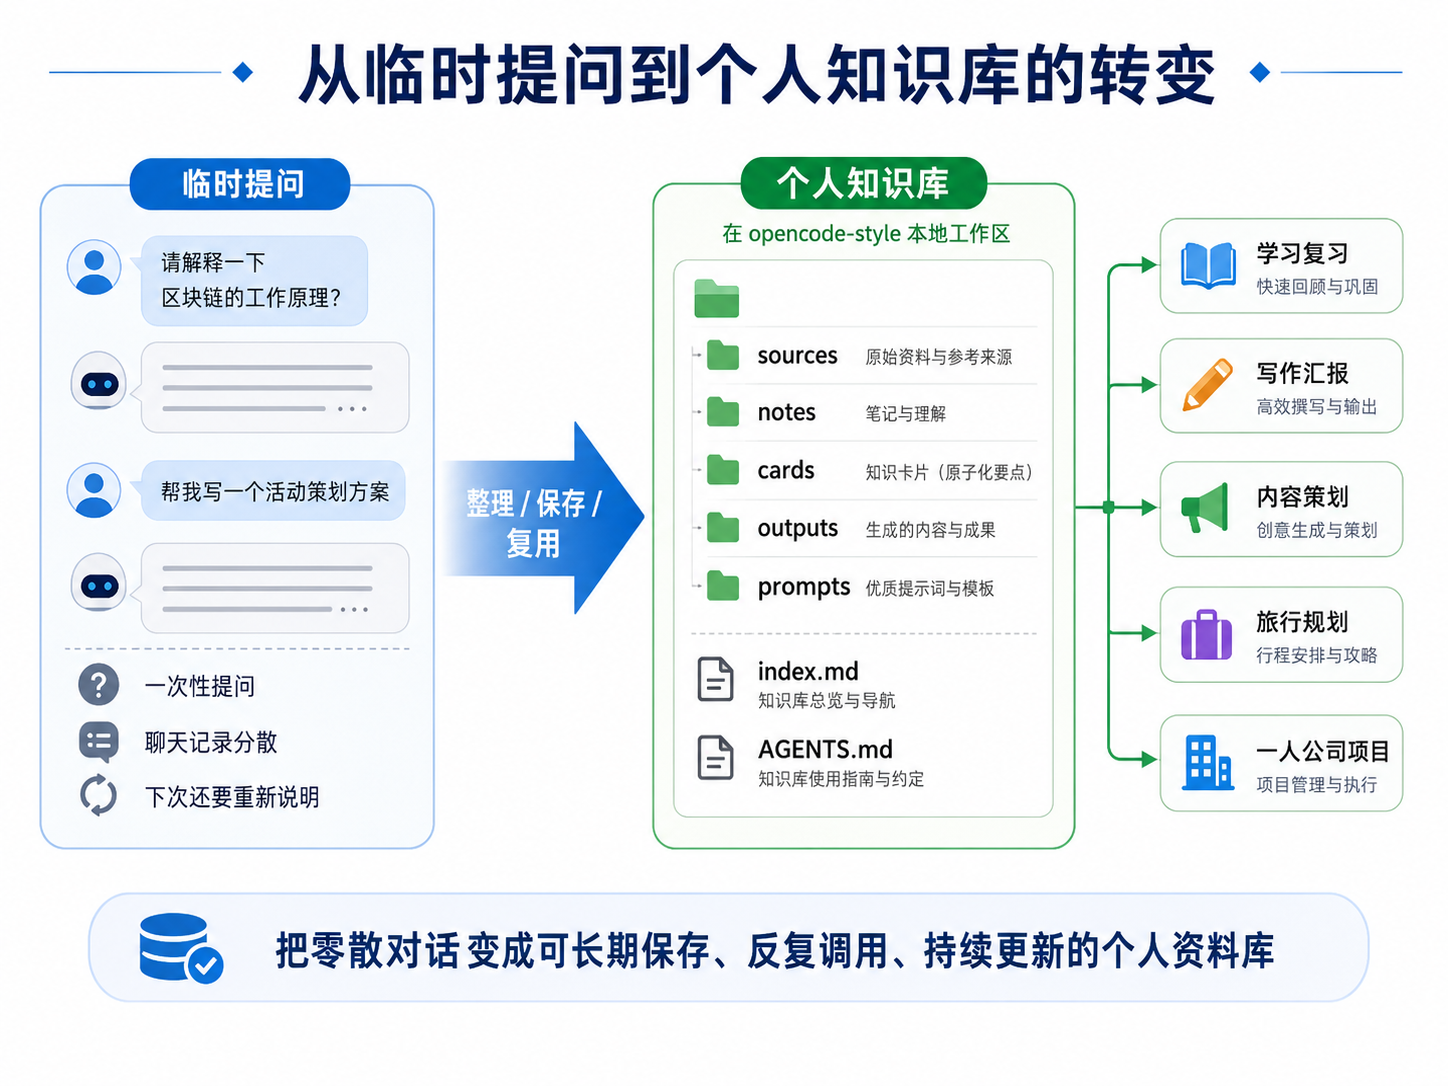
\includegraphics[width=0.88\textwidth]{images_8/个人知识库.png}
    \caption{从临时提问到个人知识库的转变}
    \label{fig:ask-to-knowledge-base}
\end{figure}
\FloatBarrier

\minorheading{最终效果：先看知识库长什么样}

搭建完成后，个人知识库不是一个复杂系统，而是一个结构清楚的本地文件夹。这个文件夹中既保存原始资料，也保存资料卡、索引、提示词和输出成果。一个最小可用的知识库可以采用下面的结构：

\begin{tcolorbox}[filebox,title=个人知识库目录结构]
\begin{verbatim}
my-knowledge-base
├── sources    原始资料
├── notes      学习笔记
├── cards      资料卡
├── outputs    生成成果
├── prompts    提示词和 Skill
├── index.md   总索引
└── AGENTS.md  opencode 工作规则
\end{verbatim}
\end{tcolorbox}

其中，\texttt{sources} 用来保存原始资料，例如文章、课堂资料、网页摘录、合同样本、技术文档等；\texttt{notes} 用来保存自己的学习笔记；\texttt{cards} 用来保存资料卡；\texttt{outputs} 用来保存 AI 辅助生成的复习提纲、脚本、方案等成果；\texttt{prompts} 用来保存常用提示词和 Skill；\texttt{index.md} 是知识库总索引；\texttt{AGENTS.md} 是写给 \texttt{opencode} 的工作规则。











   
\minorheading{创建文件夹：建立固定资料空间}

先在电脑中建立一个专门保存资料的文件夹。为了减少路径识别问题，文件夹名称建议使用英文，文件夹里的正文内容可以正常写中文。

\begin{tcolorbox}[stepbox,title=操作 1：手动创建文件夹]
打开电脑中的“文档”目录，新建一个文件夹，命名为：

\begin{verbatim}
my-knowledge-base
\end{verbatim}

然后进入这个文件夹，继续新建五个子文件夹：

\begin{verbatim}
sources
notes
cards
outputs
prompts
\end{verbatim}
\end{tcolorbox}

如果熟悉终端，也可以使用下面的命令一次性创建：

\begin{tcolorbox}[filebox,title=可选：终端命令]
\begin{verbatim}
cd ~/Documents
mkdir -p my-knowledge-base
cd my-knowledge-base
mkdir -p sources notes cards outputs prompts
\end{verbatim}
\end{tcolorbox}

这一步完成后，知识库的基本容器就建好了。接下来要做的，是告诉 \texttt{opencode}：这个文件夹不是普通代码项目，而是一个个人知识库。

\minorheading{创建规则：写好 AGENTS.md}

\texttt{AGENTS.md} 可以理解为写给 \texttt{opencode} 的“工作说明书”。它告诉 AI：回答问题前应该先看哪些文件，哪些资料不能随便修改，哪些内容不能编造，哪些结果需要人工核验。

\begin{tcolorbox}[stepbox,title=操作 2：创建工作规则文件]
在 \texttt{my-knowledge-base} 文件夹中新建一个文件，命名为：

\begin{verbatim}
AGENTS.md
\end{verbatim}

然后把下面的内容写进去。
\end{tcolorbox}

\begin{tcolorbox}[filebox,title=AGENTS.md 示例]
你是我的个人知识库助手。这个文件夹不是代码项目，而是学习和创作资料库。

工作规则：

1. 回答问题前，优先查看 index.md，再根据索引读取 sources、notes、cards 中的相关文件。

2. 回答必须说明依据来自哪个文件；如果资料中没有依据，要明确说“知识库中暂未找到依据”。

3. 不要编造来源、价格、时间、政策、法律、医疗、金融结论。

4. sources 文件夹保存原始资料，除非明确要求，不要修改。

5. notes 文件夹保存学习笔记，可以根据需要整理，但不要删除原意。

6. cards 文件夹保存资料卡，资料卡应包含来源、主题、摘要、关键词、适用场景、可提问问题和需要核验的信息。

7. outputs 文件夹保存生成成果，例如复习提纲、短视频脚本、汇报稿和内容方案。

8. prompts 文件夹保存可复用提示词和 Skill。

9. 涉及法律、金融、医疗、合同、隐私、版权和公开发布的内容，必须提醒人工核验。
\end{tcolorbox}

有了这个文件，\texttt{opencode} 在这个目录中工作时，就有了明确规则。它不应该直接凭空回答，而应先查看索引和相关资料，再给出整理结果。

\minorheading{创建索引：写好 index.md}

\texttt{index.md} 是个人知识库的总索引。它的作用类似一本书的目录：记录每份资料放在哪里、来自哪里、讲什么、以后可以回答哪些问题。没有索引，资料再多也只是堆在一起；有了索引，AI 才能更快找到应该读取的材料。

\begin{tcolorbox}[stepbox,title=操作 3：创建知识库总索引]
在 \texttt{my-knowledge-base} 文件夹中新建一个文件，命名为：

\begin{verbatim}
index.md
\end{verbatim}

然后写入下面的索引模板。
\end{tcolorbox}

\begin{tcolorbox}[filebox,title=index.md 示例]
\# 个人知识库索引

\#\# 资料登记表

| 编号 | 文件路径 | 来源/日期 | 主题 | 一句话摘要 | 标签 | 可以问的问题 | 需要核验 |
|---|---|---|---|---|---|---|---|

\#\# 使用规则

1. 回答问题前，先查看本索引。

2. 根据主题和标签找到相关 sources、notes 或 cards 文件。

3. 如果资料不足，要说明“知识库中暂未找到依据”。

4. 涉及事实、价格、政策、法律、金融、医疗、版权和公开发布内容，必须标注“需要人工核验”。
\end{tcolorbox}

以后每加入一份新资料，都要在 \texttt{index.md} 中登记。这样做看起来多了一步，但后面复习、写作、查询资料时会省很多时间。

\minorheading{放入资料：保存第一份原始材料}

第一次练习时，不建议直接放很长的 PDF 或大量图片。可以先放一段较短的文字资料，比如课堂笔记、文章摘要，或者前面整理过的“AI 学习方法”内容。这样更容易观察 \texttt{opencode} 如何读取、整理和生成资料卡。

\begin{tcolorbox}[stepbox,title=操作 4：保存第一份资料]
在 \texttt{sources} 文件夹中新建一个文件，命名为：

\begin{verbatim}
2026-05-ai-learning.md
\end{verbatim}

文件名中可以包含日期和主题，方便以后查找。不要使用“资料1”“最终版”“新建文档”这类名称。
\end{tcolorbox}

可以在文件中写入下面这段示例资料：

\begin{tcolorbox}[filebox,title=sources/2026-05-ai-learning.md 示例]
\# AI 学习方法笔记

来源：课堂整理

日期：2026 年 5 月

内容摘要：

AI 可以辅助解释概念、拆解资料、生成练习和整理复习提纲。但使用 AI 学习时，不能只复制答案，而要检查自己是否能够用自己的话解释概念、举出例子、完成类似练习，并把重要资料整理进个人知识库。
\end{tcolorbox}

这一步完成后，知识库里就有了第一份原始资料。接下来可以让 \texttt{opencode} 基于这份资料生成资料卡。

\minorheading{生成卡片：让 opencode 提炼资料卡}

资料卡相当于一份资料的“压缩说明”。它不是全文复制，而是提炼资料来源、主题、核心观点、关键词、可提问问题和需要核验的信息。以后查询知识库时，\texttt{opencode} 可以先看资料卡，再决定是否需要打开原始资料。

\begin{tcolorbox}[stepbox,title=操作 5：进入知识库并启动 opencode]
打开终端，进入刚才创建的知识库文件夹：

\begin{verbatim}
cd ~/Documents/my-knowledge-base
opencode
\end{verbatim}

如果不熟悉终端，可以先打开 \texttt{opencode}，再把当前工作目录切换到 \texttt{my-knowledge-base}。关键是让 \texttt{opencode} 在这个知识库文件夹中工作。
\end{tcolorbox}

进入 \texttt{opencode} 后，可以输入：

\begin{tcolorbox}[filebox,title=提示词或示例内容]
请阅读 @sources/2026-05-ai-learning.md，并为它生成一张资料卡。资料卡保存到 cards/2026-05-ai-learning-card.md。

资料卡必须包括：资料来源、主题、适合解决的问题、核心观点、关键词、可复习问题、需要人工核验的信息。

不要添加资料中没有出现的内容。
\end{tcolorbox}

这里的 \texttt{@sources/2026-05-ai-learning.md} 表示引用知识库中的某个文件。如果工具支持文件选择，输入 \texttt{@} 后可以按提示选择对应文件。

资料卡生成后，要打开检查一遍。重点看三点：有没有添加资料中没有的内容；有没有把不确定信息写成确定结论；关键词和可提问问题是否方便以后检索。

\minorheading{更新索引：把资料登记进目录}

资料卡生成后，还要把这份资料登记到 \texttt{index.md}。如果只生成资料卡而不更新索引，资料仍然会逐渐散掉。索引更新以后，后面提问时 \texttt{opencode} 才能先通过目录找到相关内容。

\begin{tcolorbox}[stepbox,title=操作 6：更新知识库索引]
在 \texttt{opencode} 中继续输入下面的指令，让它根据资料卡更新总索引。
\end{tcolorbox}

\begin{tcolorbox}[filebox,title=提示词或示例内容]
请根据 @cards/2026-05-ai-learning-card.md，更新 @index.md 的“资料登记表”。

新增一行，填写文件路径、来源/日期、主题、一句话摘要、标签、可以问的问题和需要核验的内容。

只更新索引，不要修改 sources 中的原始资料。
\end{tcolorbox}

更新完成后，要打开 \texttt{index.md} 看一眼：文件路径是否正确，摘要是否准确，标签是否便于以后查找，是否把不确定内容写成了确定结论。这个人工检查步骤不能省略。
\minorheading{开始提问：让 opencode 基于资料回答}

当知识库中至少有一份原始资料、一张资料卡和一个索引后，就可以开始提问。此时的关键是：不要只问“帮我总结一下”，而要明确要求 \texttt{opencode} 先查知识库，再根据资料回答，并说明依据来自哪个文件。

\begin{tcolorbox}[stepbox,title=操作 7：基于知识库提问]
在 \texttt{opencode} 中输入下面的指令，测试知识库是否能够被调用。
\end{tcolorbox}

\begin{tcolorbox}[filebox,title=提示词或示例内容]
请先查看 @index.md，再根据知识库中的资料回答：我现在想复习 AI 学习方法，哪些资料最相关？请列出依据文件，并说明每份资料适合解决什么问题。
\end{tcolorbox}

也可以继续输入：

\begin{tcolorbox}[filebox,title=提示词或示例内容]
请基于我的个人知识库，帮我整理一份“AI 辅助学习”的复习提纲。要求说明依据来自哪些 cards 或 sources 文件。如果知识库中没有依据，请明确说明，不要凭空补充。
\end{tcolorbox}

如果以后知识库中加入了家乡旅游、短视频脚本、出行准备、菜单翻译、资料整理等内容，也可以让 \texttt{opencode} 基于这些已有资料继续生成新的成果。例如：

\begin{tcolorbox}[filebox,title=提示词或示例内容]
请基于我的知识库，查找与“家乡旅游宣传素材”有关的资料，并帮我整理可用素材、可生成内容和需要人工核验的信息。
\end{tcolorbox}

这样，知识库就不只是保存资料，而是可以被调用、被追问、被复用。
\minorheading{保存提示词：沉淀常用流程}

如果经常让 \texttt{opencode} 做同一类事情，就可以把提示词保存到 \texttt{prompts} 文件夹中。这样以后不必每次重新写完整指令，只需要打开对应提示词，再替换文件名或任务主题即可。

\begin{tcolorbox}[stepbox,title=操作 8：保存资料卡生成提示词]
在 \texttt{prompts} 文件夹中新建一个文件，命名为：

\begin{verbatim}
make-card.md
\end{verbatim}

然后写入下面内容。
\end{tcolorbox}

\begin{tcolorbox}[filebox,title=prompts/make-card.md 示例]
请阅读用户指定的 sources 文件，并生成资料卡。

资料卡保存到 cards 文件夹。

资料卡必须包括：

1. 资料来源

2. 主题

3. 适合解决的问题

4. 核心观点

5. 关键词

6. 可复习问题

7. 需要人工核验的信息

要求：

- 不添加资料中没有出现的内容。

- 不确定内容标注“需要核验”。

- 不修改 sources 中的原始资料。
\end{tcolorbox}

以后需要生成资料卡时，就可以让 \texttt{opencode} 读取这份提示词，再补充具体文件名。常用流程还可以继续整理成 Skill，例如“资料卡生成助手”“知识库索引更新助手”“学习资料整理助手”。

\begin{figure}[H]
    \centering
    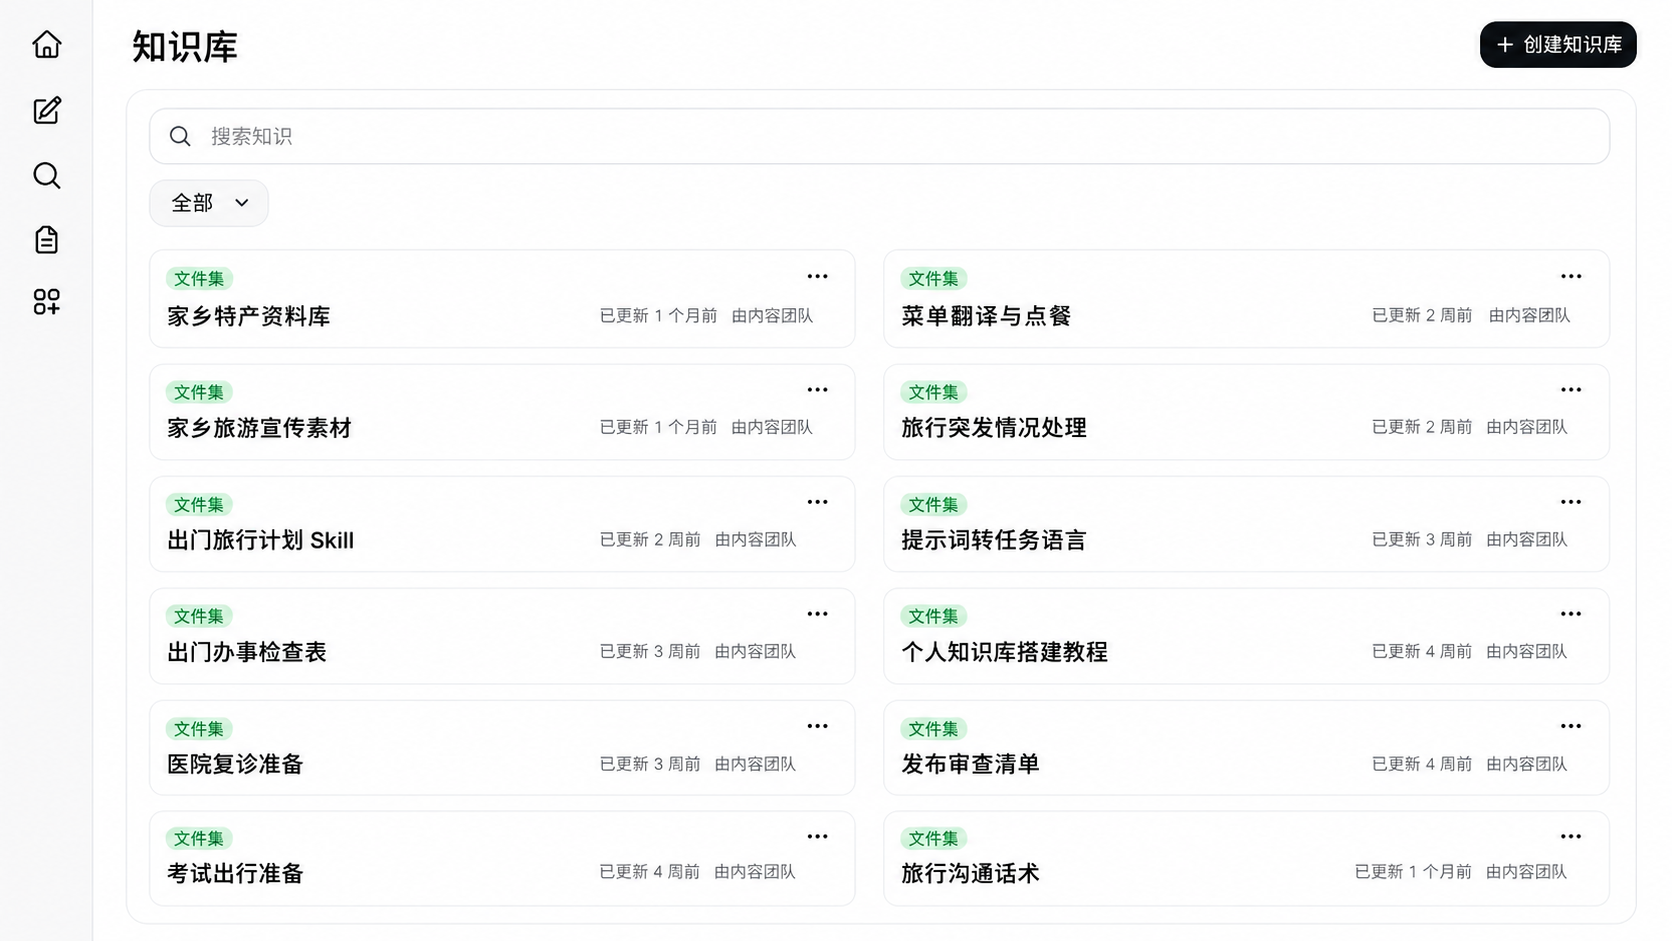
\includegraphics[width=0.88\linewidth]{ChatGPT Image 2026年5月27日 16_51_10.png}
    \caption{个人知识库展示}
    \label{fig:placeholder}
\end{figure}

\minorheading{安全边界：保护隐私与敏感资料}

个人知识库搭好以后，可以按照固定流程使用：

\begin{tcolorbox}[filebox,title=个人知识库日常流程]
\begin{verbatim}
新资料进入 sources
        ↓
生成资料卡到 cards
        ↓
更新 index.md
        ↓
基于知识库提问
        ↓
有价值的输出保存到 outputs
        ↓
常用提示词保存到 prompts
\end{verbatim}
\end{tcolorbox}

比如，今天保存了一篇关于 AI 学习方法的文章，明天可以让 \texttt{opencode} 生成资料卡并更新索引；后天要写学习总结时，就可以让 \texttt{opencode} 先查索引，再基于资料卡生成提纲。这样，学习不再是一次次零散提问，而是逐步形成一个可以积累、查询和复用的个人知识系统。

\begin{tcolorbox}[warnbox]
个人知识库越用越久，里面可能会保存证件号码、手机号、家庭住址、订单截图、合同内容、客户资料、公司文件等敏感信息。放入知识库前，应先判断是否需要脱敏。涉及身份证、护照、银行卡、验证码、病历、合同敏感条款、客户名单和未公开项目资料时，不要直接原样放入。涉及法律、金融、医疗、合同、版权和公开发布的内容，知识库只能辅助理解和整理，不能替代专业判断。
\end{tcolorbox}

个人知识库的价值，不在于文件数量有多少，而在于资料是否清楚、来源是否可靠、索引是否好用、能否被 AI 正确调用。以后无论是学习复习、写作汇报、制作家乡旅游宣传视频，还是继续搭建更复杂的个人智能体，都可以在这个知识库基础上扩展。
% ====================== 8.4 ======================


% ============================================================
% 8.4 求职沟通与简历优化
% ============================================================

\section{工作协作与职业发展}

\subsection{履历呈现与自我展示}

过去谈到简历，很多人会觉得它只是“把自己的经历写清楚”。但在 AI 已经进入招聘流程之后，简历不再只是写给人看的材料，也可能会先被算法读取、筛选和排序。换句话说，求职者不仅要让招聘者看懂自己，也要让招聘系统更准确地识别自己的经历与岗位之间的匹配关系。

《AI Self-preferencing in Algorithmic Hiring》这项研究就提出了一个值得注意的现象：当求职者使用 AI 修改简历，而企业也使用大语言模型筛选简历时，招聘模型可能更偏好 AI 生成或同类模型生成的简历。研究者在模拟招聘流程中发现，在资质相同的情况下，使用同类大语言模型修改简历的候选人，进入候选名单的概率比提交人工简历的候选人高 23\%—60\%。这说明，AI 辅助求职已经不只是“润色几句话”，还涉及简历表达风格、岗位关键词、平台筛选机制和算法偏好的适配问题。

\begin{figure}[H]
    \centering
    
\includegraphics[width=0.88\textwidth]{\detokenize{images_8/当AI招聘遇上AI简历_系统性的偏好.png}}
    \caption{当 AI 招聘遇上 AI 简历：系统性的偏好}
    \label{fig:ai-hiring-preference}
\end{figure}

这并不是鼓励读者用 AI 编造经历，而是提醒大家：在新的求职环境中，真实经历也需要被更清楚、更结构化地表达出来。如果简历只是写“参与活动”“负责沟通”“完成项目”，招聘者和系统都很难判断你的真实能力；如果能写清楚任务背景、本人职责、使用方法和实际结果，简历就会更容易被理解。AI 的正确作用，是帮助读者把真实经历整理成更准确、更有岗位匹配度的表达，而不是把没有做过的事情包装成经历。

\subsubsection*{先读懂岗位，再开始写简历}

很多人使用 AI 写简历时，一上来就输入：“帮我写一份简历。”这种做法通常效果不好。因为简历不是孤立存在的，它必须和目标岗位相匹配。同样一段经历，投新媒体运营、行政助理、教师助理、Java 开发、销售岗位时，应该突出完全不同的能力。

求职准备的第一步，是把岗位要求读懂。读者可以把招聘信息提供给 AI，然后输入：

\begin{tcolorbox}[promptbox]
请帮我分析这份岗位要求。请提取岗位核心职责、必须具备的能力、加分项、简历中应该重点体现的关键词，以及面试时可能被追问的问题。请用表格输出，并区分“必须体现”和“可以加分”的内容。
\end{tcolorbox}

例如，一份岗位要求中写着“负责活动策划与执行、社群维护、用户反馈整理、基础数据统计”，AI 就可以帮助读者拆出几个核心能力：活动执行能力、沟通协调能力、信息整理能力、数据意识和用户服务意识。这样，后面修改简历时，就不再是泛泛地写“本人沟通能力强”，而是要用真实经历证明这些能力。

英国 National Careers Service 在简历建议中也强调，简历应当根据申请岗位进行调整，结合岗位说明、必要条件和公司信息来匹配内容，同时更新新的成就、经历和技能，删除过时信息。 这说明，简历不是一份材料投所有岗位，而是要根据岗位不断调整重点。

\subsubsection*{把自己的经历整理成可用素材}

读懂岗位以后，第二步是整理自己的经历。很多读者觉得自己“没什么可写”，其实往往不是没有经历，而是没有把经历拆开。一次课程项目、社团活动、志愿服务、实习任务、兼职经历、比赛作品、公众号运营、毕业设计，都可能包含可以写进简历的内容。

整理经历时，可以让 AI 帮忙搭一个表格。输入：

\begin{tcolorbox}[promptbox]
我准备申请【岗位名称】。下面是我做过的一些真实事情，请帮我判断哪些经历适合写进简历，并整理成“任务背景—我负责什么—使用了什么方法—形成了什么结果—对应岗位能力”的表格。注意：只能基于我提供的信息，不要编造数据和经历。
\end{tcolorbox}

然后补充真实经历，例如：

\begin{tcolorbox}[promptbox]
我参加过学院迎新活动，负责新生群通知、报名表收集和现场签到。
我做过课程小组作业，负责资料整理和 PPT 制作。
我运营过班级公众号，写过 5 篇推文。
我会用 Excel 做简单统计，也会用剪映剪视频。
\end{tcolorbox}

AI 可以帮助读者发现，这些经历并不是“没什么可写”。“负责新生群通知”可以体现信息传达和社群沟通；“报名表收集”可以体现资料整理和表格处理；“现场签到”可以体现活动执行和现场协调；“公众号推文”可以体现内容写作和平台运营。经过整理以后，原本零散的经历就能变成简历素材。

\begin{figure}[H]
    \centering
    
\includegraphics[width=0.88\textwidth]{\detokenize{images_8/简历经历整理_AI界面示例.png}}
    \caption{AI 辅助整理简历经历匹配表格示例}
    \label{fig:resume-experience-match}
\end{figure}

这里要注意，AI 可以帮助挖掘真实经历中的价值，但不能虚构没有发生过的内容。如果没有负责数据分析，就不能写成“独立完成数据分析”；如果只是参与活动，就不能写成“主导活动策划”；如果没有统计结果，就不能让 AI 编造“提升 50\%”“覆盖 1000 人”“转化率显著提高”。简历是面试时会被追问的材料，真实性比漂亮表达更重要。

\subsubsection*{把经历改写成简历语言}

简历语言不需要华丽，但要具体、清楚、能证明能力。比较实用的写法是：动作 + 任务 + 方法 + 结果。如果有真实数据，可以写数据；如果没有数据，也可以写清楚完成了什么产出、服务了什么对象、承担了什么职责。

普通写法：
\begin{quote}
参与学校迎新活动。
\end{quote}

优化后：
\begin{quote}
参与学院迎新活动，负责新生群通知、报名信息收集和现场签到协助，帮助新生完成报到流程。
\end{quote}

如果有真实数据，可以进一步写成：
\begin{quote}
参与学院迎新活动，负责 3 个新生群的信息通知、报名表收集和现场签到协助，整理 300 余条报名信息，帮助新生顺利完成报到流程。
\end{quote}

这两种写法都没有编造经历，但第二种更具体，第三种在有真实数据的情况下更有说服力。AI 可以帮助读者把“我做过什么”改成“这件事体现了什么能力”。

可以输入：

\begin{tcolorbox}[promptbox]
请帮我把下面这段经历改写成适合简历的表达。要求：语言简洁，突出我负责的工作、使用的方法和体现的能力；如果没有明确数据，不要编造，请提醒我哪些地方可以补充真实数据。
原始经历：【粘贴经历】
\end{tcolorbox}

AI 输出后，读者要逐句检查。凡是出现“主导”“统筹”“独立负责”“显著提升”“大幅增长”等词，都要确认是否符合真实情况。如果自己只是协助，就写“协助”；如果只是参与，就写“参与”；如果确实负责某个模块，再写“负责”。简历表达可以优化，但职责边界不能随意升级。

\subsubsection*{根据不同岗位定制简历重点}

同一份基础简历，不适合直接投所有岗位。比如，一个学生有“活动组织、公众号运营、课程项目、Excel 统计”几类经历。投新媒体运营时，应重点写公众号、文案、选题、平台发布和数据反馈；投行政助理时，应重点写材料整理、活动协调、表格统计、流程执行；投销售助理时，应重点写客户沟通、信息记录、问题反馈和跟进意识。

这时可以让 AI 做岗位匹配分析：

\begin{tcolorbox}[promptbox]
我有一份基础简历和一个目标岗位 JD。请帮我做岗位匹配分析：
这个岗位最看重哪些能力；
我的简历中哪些内容最匹配；
哪些经历应该放在更靠前的位置；
哪些表达需要改得更具体；
哪些内容与岗位关系不大，可以弱化。
注意：不要编造经历，只能基于我提供的材料提出修改建议。
\end{tcolorbox}

AI 的价值在于帮助读者“重新排序”和“突出重点”。它不是简单把简历写长，而是帮助判断：哪些经历最应该放在前面，哪些关键词应该出现，哪些内容可以删减。LinkedIn 工程博客介绍，其 AI-powered job search 已经允许用户用自然语言描述想找的工作，并根据理想岗位返回更匹配的结果，这也说明求职正在从传统关键词匹配，逐渐走向更强的语义匹配和意图理解。

因此，读者在修改简历时，也要学会从“堆关键词”转向“表达匹配关系”。岗位要求“活动执行”，简历中就要有真实活动经历；岗位要求“数据整理”，简历中就要体现表格、统计、整理和反馈；岗位要求“客户沟通”，简历中就要体现沟通对象、沟通内容和处理结果。

\subsubsection*{写好个人总结和求职信}

很多简历开头会有“个人总结”或“求职意向”。这部分不能写成空泛评价，例如“本人性格开朗、吃苦耐劳、学习能力强”。更好的写法是用两三句话说明自己的背景、目标岗位和最相关优势。

可以让 AI 帮助生成个人总结：

\begin{tcolorbox}[promptbox]
请根据我的经历和目标岗位，帮我写一段 80 字以内的简历个人总结。要求：突出与岗位最相关的 2—3 个能力，不要写空话，不要使用“吃苦耐劳、认真负责”这类泛泛表达。
\end{tcolorbox}

如果申请场景需要求职信，也可以输入：

\begin{tcolorbox}[promptbox]
我准备申请【岗位名称】，下面是岗位要求和我的经历。请帮我生成一版 300 字以内的求职信初稿。内容包括：我为什么申请这个岗位、我有哪些相关经历、我能为团队带来什么。语气正式但自然，不要夸张，不要编造经历。
\end{tcolorbox}

求职信不是重复简历，而是把“岗位需求”和“个人经历”连接起来。例如，可以写自己为什么对这个方向感兴趣，过去哪段经历与岗位相关，自己希望如何在岗位中继续发挥作用。AI 可以生成初稿，但最终要改成自己的语言，避免所有人都写出相似的 AI 味表达。

\subsubsection*{准备面试自我介绍}

简历通过筛选后，面试通常会先要求自我介绍。很多读者的自我介绍容易出现两个问题：一种是太短，只说姓名、学校、专业；另一种是太长，把简历从头到尾背一遍。更合适的自我介绍应该围绕目标岗位展开，一般包括三个部分：基本背景、相关经历、岗位兴趣。

可以输入：

\begin{tcolorbox}[promptbox]
请根据我的简历和目标岗位，帮我准备一段 1 分钟中文自我介绍。要求：先说明我的背景，再突出 2 个与岗位最相关的经历，最后表达我对岗位的兴趣。语言自然，不要像背稿。
\end{tcolorbox}

AI 生成后，还可以继续优化：

\begin{tcolorbox}[promptbox]
这版自我介绍有点书面化，请改成更适合面试现场说出来的版本，句子短一点，语气自然一点，不要使用夸张词。
\end{tcolorbox}

准备自我介绍时，读者要注意两点。第一，不要把所有经历都塞进去，只讲和岗位最相关的经历。第二，不要背诵 AI 生成稿，而要理解结构后用自己的话表达。面试官更希望听到真实、清楚、有重点的表达，而不是一段过度包装的标准答案。

\subsubsection*{用 AI 做面试问题预测和模拟练习}

AI 在面试准备中很有用。它可以根据岗位要求和简历内容，预测面试官可能会问什么问题，也可以根据读者的回答给出修改建议。

可以输入：

\begin{tcolorbox}[promptbox]
请根据我的简历和目标岗位，帮我预测 10 个面试问题。请分成三类：岗位能力问题、项目经历追问、综合素质问题。每个问题后面说明面试官想考察什么，以及我应该用哪段经历回答。
\end{tcolorbox}

常见问题包括：
\begin{itemize}
    \item 你为什么申请这个岗位？
    \item 你最能体现沟通能力的一段经历是什么？
    \item 你在项目中遇到过什么困难？怎么解决？
    \item 如果临时任务很多，你会如何安排优先级？
    \item 你对这个岗位的理解是什么？
\end{itemize}

回答经历类问题时，可以用“情境—任务—行动—结果”的结构。也就是先说当时是什么情况，再说自己负责什么，接着说采取了什么行动，最后说结果如何、学到了什么。

\begin{figure}[H]
    \centering
    
\includegraphics[width=0.88\textwidth]{\detokenize{images_8/面试问题预测_AI界面示例.png}}
    \caption{AI 辅助预测面试问题并分类示例}
    \label{fig:interview-question-prediction}
\end{figure}

可以输入：

\begin{tcolorbox}[promptbox]
请用“情境—任务—行动—结果”的结构，帮我整理下面这个经历，变成适合面试回答的版本。要求真实、简洁、口语化，不要编造数据。
经历：【粘贴经历】
\end{tcolorbox}

还可以让 AI 扮演面试官：

\begin{tcolorbox}[promptbox]
请你扮演面试官，针对我申请的【岗位名称】进行模拟面试。一次只问一个问题。等我回答后，请从内容完整性、表达清晰度、岗位匹配度三个方面给我反馈，并提出修改建议。
\end{tcolorbox}

这种练习的意义，不是背出完美答案，而是发现自己的表达问题。比如回答是否太空、是否没有说结果、是否没有体现岗位能力、是否回答偏题。经过几轮练习后，读者会更清楚自己应该讲哪段经历、怎么讲、讲到什么程度。

\subsubsection*{检查 AI 生成内容中的风险}

AI 可以提高求职准备效率，但也可能带来风险。最常见的问题是：表达过度包装，经历被夸大，数据被编造，职责被升级，关键词被堆砌。简历看起来更强了，但面试时解释不了，反而会降低信任。

使用 AI 优化简历后，读者要逐项检查：
\begin{itemize}
    \item 第一，经历是否真实。自己没有做过的内容必须删除。
    \item 第二，职责是否准确。参与、协助、负责、主导，不能混用。
    \item 第三，数据是否可靠。没有统计过的数据不能编造。
    \item 第四，技能是否掌握。不会的工具、语言、平台不能写成熟练。
    \item 第五，表达是否能解释。简历上每一句话，都要能在面试中讲清楚。
\end{itemize}

还要注意隐私保护。上传简历给 AI 前，可以隐藏身份证号、详细住址、完整手机号、证件号码、公司内部资料、未公开项目数据等敏感信息。AI 可以帮你修改表达，但不需要知道所有个人隐私。




\subsection{会议协作：会前准备、会中记录与会议纪要}

很多人一听到“开会”，第一反应就是“坐在那里听别人说话”。但真正进入学习、实习和工作以后就会发现，会议并不是简单地把人聚在一起，而是一个非常典型的协作场景。一次会议如果准备不好，就容易变成大家各说各的；记录不好，开完以后谁也记不清刚才到底定了什么；纪要写不好，就会出现“会上好像说过”“我以为不是我负责”“这个时间不是下周吗”之类的问题。

AI 在会议场景中的价值，正是帮助我们把会议从“说过了”变成“说清楚了”，再进一步变成“可以执行了”。现在许多办公工具已经把 AI 会议能力做进产品中。例如，Microsoft Teams 中的 Copilot 可以总结会议讨论重点，说明谁说了什么，并建议行动项；Google Meet 中的 Gemini “Take notes for me” 可以捕捉会议笔记和行动项，并生成 Google Docs 文档；Zoom AI Companion 也支持生成会议摘要和后续步骤，并在会议结束后发送摘要。 这些功能说明，AI 会议助手已经不再是概念，而是在真实办公场景中帮助人们减少漏记、整理重点和推进协作。

% \begin{figure}[H]
%     \centering
%     \includegraphics[width=0.88\textwidth]{\detokenize{AI会议协作流程示意图.png}}
%     \caption{AI 会议协作：从语音到可执行结果的流程}
%     \label{fig:meeting-collaboration-flow}
% \end{figure}

不过，会议使用 AI 不能只理解成“开完会自动生成纪要”。一场真正有效的会议，通常包括三个阶段：会前准备、会中记录、会后纪要。本小节重点学习这三个阶段如何使用 AI，让会议更有方向、更有记录、更有结果。

\subsubsection*{会前准备：先把“为什么开会”说清楚}

很多低效会议的问题，其实在会议开始前就已经埋下了。比如会议通知只写“明天下午开会讨论活动方案”，但没有说明讨论什么、需要谁准备材料、会议要形成什么结果。到了会议现场，大家只能临时回忆：活动预算是多少？场地定了吗？谁负责宣传？这次到底是讨论方案，还是拍板决定？这样一来，会议很容易越开越散。

会前使用 AI 的第一步，是让它帮助我们整理会议目标。会议目标不是“开个会”，而是要回答三个问题：这次会议为什么开？需要讨论哪些问题？会议结束时希望得到什么结果？如果这三个问题不清楚，再先进的 AI 会议工具也只能记录一堆散乱发言。

例如，准备一次“校园活动策划会”时，可以这样输入：

\begin{tcolorbox}[promptbox]
我准备组织一次校园活动策划会议。已知活动主题是“AI 学习分享会”，参会人员包括活动负责人、宣传同学、场地对接同学和主持人。请帮我整理会前准备内容，包括会议目标、建议议题、每个议题需要提前准备的材料，以及会议结束时应该形成哪些结论。
\end{tcolorbox}

AI 可以帮助生成一份会前提纲，比如：

\begin{table}[H]
\centering
\caption{校园活动策划会会前提纲}
\label{tab:meeting-pre-outline}
\begin{tabular}{p{0.25\linewidth} p{0.65\linewidth}}
\toprule
\textbf{模块} & \textbf{内容} \\
\midrule
会议目标 & 明确活动时间、地点、宣传方式、人员分工和后续时间表 \\
议题一 & 活动主题和目标受众是否明确 \\
议题二 & 场地、设备和时间是否可行 \\
议题三 & 宣传渠道、推文发布时间和报名方式 \\
议题四 & 主持人、嘉宾、签到、摄影等分工 \\
会议产出 & 活动方案定稿、任务分工表、截止时间和下一次确认节点 \\
\bottomrule
\end{tabular}
\end{table}

这样的会前准备，比只写一句“讨论活动方案”更有效。它让参会者提前知道会议要解决什么问题，也让会议主持人知道应该按什么顺序推进。

如果是项目组会议，也可以输入：

\begin{tcolorbox}[promptbox]
我们明天要开项目进度会，项目是【项目名称】。请帮我设计一份会议议程，要求包括：当前进展汇报、遇到的问题、需要协调的资源、下一阶段任务和风险提醒。请输出一份适合发给参会人员的会前通知。
\end{tcolorbox}

AI 可以生成更完整的会议通知：

\begin{quote}
各位好，明天下午 3 点召开项目进度会。本次会议主要确认当前进展、存在问题和下一阶段任务安排。请各负责人提前准备以下内容：已完成事项、未完成事项、遇到的困难、需要其他成员配合的部分，以及下周计划。会议结束时将形成任务分工表和截止时间。
\end{quote}

这类内容看起来简单，但能大幅减少会议中的无效沟通。因为每个人都知道自己需要带着什么信息来开会。

\subsubsection*{会前材料整理：让 AI 帮你先读一遍资料}

有些会议不是从零开始讨论，而是基于已有材料继续推进，比如项目文档、调研报告、用户反馈、活动方案、会议记录、客户需求清单等。如果参会者没有提前读材料，会议就会变成“现场读文档”。AI 可以帮助我们在会前快速整理材料，提炼重点问题。

可以把会议材料提供给 AI，然后输入：

\begin{tcolorbox}[promptbox]
请阅读这份会议材料，帮我整理会前速读笔记。请包括：材料主要内容、已经明确的结论、仍然不清楚的问题、会议中需要重点讨论的事项，以及我应该提前准备的发言要点。
\end{tcolorbox}

\begin{figure}[H]
    \centering
    
\includegraphics[width=0.88\textwidth]{\detokenize{images_8/会前材料整理_AI界面示例.png}}
    \caption{AI 辅助整理会议材料重点与待讨论事项示例}
    \label{fig:pre-meeting-material-sort}
\end{figure}

AI 输出后，读者可以重点看两类内容：一类是“已经明确的信息”，比如活动时间、项目目标、客户需求；另一类是“仍然需要讨论的信息”，比如预算没确定、负责人没明确、风险没有处理方案。这样，会议就不会浪费大量时间重复已经清楚的内容，而是把时间留给真正需要讨论的问题。

如果是学生小组作业，也可以这样使用：

\begin{tcolorbox}[promptbox]
下面是我们小组目前的作业资料。请帮我整理下一次小组会议要讨论的问题。要求区分：已经完成的部分、需要补充的部分、需要组员共同决定的部分，以及我可以在会上汇报的内容。
\end{tcolorbox}

这样，AI 不只是帮忙总结资料，还能帮读者找到“会上该说什么”。很多人开会时不知道怎么发言，其实不是没有想法，而是没有提前把材料和问题整理出来。

\subsubsection*{会前发言准备：让表达更有条理}

会议中，很多人发言容易出现两种情况：一种是太短，只说“我这边没问题”；另一种是太散，说了很多细节，但别人听不出重点。会前可以让 AI 帮自己准备发言提纲，让表达更清楚。

例如，项目进度汇报可以使用这个提示：

\begin{tcolorbox}[promptbox]
我需要在项目会议上汇报自己的进展。请根据下面的信息帮我整理一段 1 分钟发言。要求包括：已完成事项、当前问题、下一步计划和需要协助的地方。语言自然，适合会议现场表达，不要写得像正式文章。
我的信息是：【粘贴自己的进展记录】
\end{tcolorbox}

AI 可以把零散记录整理成这样的发言：

\begin{quote}
我这边本周主要完成了报名表设计和活动推文初稿，目前报名表已经可以使用，推文还需要补充嘉宾介绍。现在主要问题是嘉宾简介还没有最终确认，所以宣传发布时间可能会受到影响。下一步我会先完善推文结构，同时等嘉宾信息确认后补充内容。需要大家协助的是，负责嘉宾对接的同学最好在明天下午前给我最终版简介。
\end{quote}

这样的发言有四个要素：完成了什么、遇到什么问题、下一步做什么、需要谁协助。它比“我这边还在做推文”更清楚，也更容易让会议产生结果。

如果读者要在客户会议中发言，语气还要更谨慎。可以输入：

\begin{tcolorbox}[promptbox]
请帮我把下面这段内部表达改成适合客户会议的发言。要求：语气专业、不过度承诺，清楚说明目前进展、可交付内容和需要客户确认的问题。
\end{tcolorbox}

这种用法可以帮助读者区分内部沟通和外部沟通。内部会议可以直接说问题，客户会议则要更注意表达方式，既要说明进展，也不能随意承诺无法确认的结果。

\subsubsection*{会中记录：不要只记“谁说了什么”，还要记“会议形成了什么”}

会议开始以后，AI 可以帮助记录，但记录不是把所有话一字不落写下来。真正有用的会议记录，应该能回答几个问题：会议讨论了什么？形成了哪些结论？哪些问题还没解决？谁负责什么？什么时候完成？哪些内容需要会后确认？

现在很多会议工具已经在这方面提供支持。Teams 中的 Copilot 可以在会议中或会后总结讨论重点、回答关于会议内容的问题，并建议行动项；Google Meet 的“Take notes for me”会将会议记录和后续事项组织到文档中，并可附加到日历事件，便于参会者后续访问；Zoom 的 AI Companion Meeting Summary 可以在主持人启用后生成会议摘要，会议结束后发送总结内容。

但在实际学习和工作中，不是每个人都能使用这些高级办公工具。有时只是线下小组会，有时只是普通语音会议，有时只有自己手动记录。即使没有自动会议助手，也可以用 AI 参与会中记录的后半段：先由人记录要点，再让 AI 整理结构。

会中记录时，可以按照下面这个格式记：

\begin{table}[H]
\centering
\caption{会中记录项目}
\label{tab:meeting-record-items}
\begin{tabular}{p{0.25\linewidth} p{0.65\linewidth}}
\toprule
\textbf{记录项目} & \textbf{应记录内容} \\
\midrule
讨论主题 & 这部分在讨论什么问题 \\
主要观点 & 各方提出了哪些看法 \\
已定结论 & 哪些事情已经确定 \\
待确认问题 & 哪些事情还没有确定 \\
任务分工 & 谁负责什么 \\
截止时间 & 什么时候完成 \\
风险提醒 & 可能影响进度的问题 \\
\bottomrule
\end{tabular}
\end{table}

比如，在一次活动策划会上，原始记录可能很乱：
\begin{quote}
宣传要提前发。海报小王负责。报名表还没做好。场地可能要换。老师说周三前要确定嘉宾。主持人还没定。预算要再问一下。
\end{quote}

这段记录虽然有信息，但不适合直接作为纪要。可以会后输入：

\begin{tcolorbox}[promptbox]
请把下面这段会议记录整理成结构化会议纪要。要求包括：会议主题、主要结论、任务分工、截止时间、待确认问题和风险提醒。不要编造没有出现的信息，不能确定的内容标注“待确认”。
原始记录：【粘贴记录】
\end{tcolorbox}

AI 可以整理成：

\begin{table}[H]
\centering
\caption{结构化会议纪要示例}
\label{tab:structured-meeting-minutes-example}
\begin{tabular}{p{0.25\linewidth} p{0.65\linewidth}}
\toprule
\textbf{类别} & \textbf{内容} \\
\midrule
会议主题 & 活动策划推进会 \\
已定事项 & 宣传需要提前发布；海报由小王负责；嘉宾需在周三前确认 \\
待完成任务 & 完成报名表；确认主持人；核实预算；确认场地是否变更 \\
风险提醒 & 场地可能变更，可能影响宣传信息；嘉宾未确认会影响推文发布时间 \\
待确认问题 & 最终场地、预算金额、主持人人选 \\
\bottomrule
\end{tabular}
\end{table}

这样，原本散乱的口头讨论就变成了可以检查的会议记录。

\subsubsection*{会议纪要：把讨论变成可追踪的结果}

会议纪要不是会议录音的文字版，也不是把每个人说过的话全部抄下来。纪要的作用是留下清楚、简洁、可追踪的会议结果。一个好的会议纪要，至少应包括六个部分：会议基本信息、会议主题、主要讨论内容、形成的结论、任务分工、待确认问题。

可以使用这个模板：

\begin{tcolorbox}[promptbox]
请根据下面的会议记录生成会议纪要。
纪要结构包括：
会议名称、时间、参会人员；
会议目标；
主要讨论内容；
已形成的结论；
任务分工表，包括任务、负责人、截止时间；
待确认问题；
下一次会议建议议题。
要求语言正式、简洁，不要编造未提到的信息，责任人和截止时间不明确的地方标注“待确认”。
\end{tcolorbox}

生成后的会议纪要可以这样呈现：

\begin{table}[H]
\centering
\caption{会议纪要模块示例}
\label{tab:meeting-minutes-module-example}
\begin{tabular}{p{0.25\linewidth} p{0.65\linewidth}}
\toprule
\textbf{模块} & \textbf{内容} \\
\midrule
会议名称 & AI 学习分享会筹备会议 \\
会议目标 & 确认活动方案、宣传安排和任务分工 \\
主要结论 & 活动初步定于下周五下午；宣传推文需提前三天发布；报名表本周内完成 \\
任务分工 & 小王负责海报；小李负责报名表；小张负责联系嘉宾；主持人待定 \\
截止时间 & 嘉宾信息周三前确认；报名表周五前完成 \\
待确认问题 & 场地是否变更；预算金额；主持人人选 \\
风险提醒 & 场地和嘉宾未确认可能影响宣传发布时间 \\
\bottomrule
\end{tabular}
\end{table}

这样的纪要适合发给参会人员，也适合作为后续跟进的依据。它不是简单“会议记录”，而是会议成果的整理。

需要注意，AI 生成纪要后，读者不能直接发送。要重点核对四类信息：责任人是否准确，截止时间是否准确，结论是否真实达成，待确认事项是否被误写成已确定事项。AI 可能把“有人建议”误整理成“会议决定”，也可能把“下周再看”误整理成“下周完成”。所以，纪要发出前必须人工检查。

\subsubsection*{不同会议类型，纪要重点也不同}

会议不是只有一种。不同会议的记录重点不同，AI 提示也要随之调整。

如果是项目进度会，重点是任务推进：
\begin{tcolorbox}[promptbox]
请把会议记录整理成项目进度纪要，重点提取：已完成事项、未完成事项、问题阻塞、负责人、截止时间和需要协调的资源。
\end{tcolorbox}

如果是头脑风暴会，重点是想法分类：
\begin{tcolorbox}[promptbox]
请把会议记录整理成头脑风暴纪要，重点提取：提出的想法、可行性较高的方案、需要进一步验证的问题、暂不采用的想法及原因。
\end{tcolorbox}

如果是客户沟通会，重点是需求和承诺：
\begin{tcolorbox}[promptbox]
请把会议记录整理成客户沟通纪要，重点提取：客户需求、客户关注点、我方回应、已确认事项、未承诺事项、后续需要客户确认的问题。凡是涉及价格、交付时间、合同条款和服务承诺的内容，请标注“需要人工确认”。
\end{tcolorbox}

如果是学习讨论会，重点是知识点和疑问：
\begin{tcolorbox}[promptbox]
请把会议记录整理成学习讨论纪要，重点提取：本次讨论的知识点、不同观点、未解决问题、需要查阅的资料和下次讨论任务。
\end{tcolorbox}

通过这些例子可以看出，AI 不是只会生成一种固定格式的会议纪要。读者要先判断会议类型，再告诉 AI 应该重点提取什么。项目会议看任务，客户会议看需求和承诺，学习会议看知识点和疑问，头脑风暴看想法和后续验证。

\subsubsection*{AI 会议记录的使用边界}

会议往往包含内部信息、客户信息、项目数据、价格方案、合作条款和个人发言，因此使用 AI 时必须注意边界。不是所有会议内容都适合上传到公共 AI 工具中。涉及商业秘密、未公开项目、客户隐私、合同内容、个人身份信息、财务数据时，应遵守所在学校、单位或团队的规定，必要时先做脱敏处理。

例如，可以把真实客户名称改成“客户 A”，把具体金额改成“某金额”，把内部项目代号改成“项目 X”，把手机号、邮箱、身份证号、订单号等敏感信息遮挡掉。AI 生成纪要并不一定需要知道所有原始隐私信息，很多时候只需要知道事件结构和任务关系。

同时，会议录音、转写和 AI 纪要也要尊重参会者知情权。在线会议工具中的 AI 会议摘要通常需要主持人或管理员启用，Zoom 官方文档也说明，会议摘要功能可由主持人启用或停止，摘要生成后可通过邮件或聊天共享。 在实际使用中，如果要录音、转写或使用 AI 记录会议，应遵守会议组织者要求和相关制度，不要私自记录敏感会议。




\subsection{会后执行：任务跟进、工作汇报与协作闭环}

会议结束，并不代表工作结束。很多时候，真正的问题不是“会开得不够热闹”，而是“会后没有人继续推进”。会上讨论了很多想法，纪要也写出来了，但过几天再问，可能会发现：谁负责什么不清楚，截止时间没有写明，某个问题还在等确认，原本说好的材料没人跟进。这样的会议，看起来开过了，实际上没有形成工作闭环。

AI 在会后阶段的价值，就是把会议纪要进一步转化成可执行的任务、可发送的跟进消息、可检查的进度表和可复盘的工作汇报。Microsoft Teams 中的 Copilot 可以捕捉会议重点、行动项和会议结果，Google Meet 的 Gemini 也可以记录会议笔记和行动项，并将笔记文档附加到日历事件中，方便会后继续跟进。(Microsoft Support) 这说明，AI 会议协作的重点已经不只是“记下来”，而是帮助团队把会议内容继续推进下去。

\subsubsection*{把会议纪要变成任务清单}

会议纪要通常记录“会议说了什么”，但任务清单要回答“接下来谁做什么”。这两者不一样。会议纪要可以写得相对完整，任务清单则必须清楚、具体、可检查。比如纪要里写“下周继续完善宣传方案”，这句话还不能直接执行，因为它没有说明谁完善、完善哪一部分、什么时候完成、完成后交给谁确认。

会后可以把会议纪要交给 AI，要求它提取任务清单。可以这样输入：

\begin{tcolorbox}[promptbox]
请根据下面的会议纪要，提取一份会后任务清单。
要求包括：任务内容、负责人、截止时间、依赖事项、交付物、风险提醒。
如果负责人或截止时间不明确，请标注“待确认”，不要自行编造。
会议纪要：【粘贴会议纪要】
\end{tcolorbox}

AI 整理后的结果可以是这样的：

\begin{table}[H]
\centering
\caption{会后任务清单示例}
\label{tab:post-meeting-task-list-example}
\begin{tabular}{p{0.18\linewidth} p{0.10\linewidth} p{0.10\linewidth} p{0.12\linewidth} p{0.18\linewidth} p{0.22\linewidth}}
\toprule
\textbf{任务内容} & \textbf{负责人} & \textbf{截止时间} & \textbf{交付物} & \textbf{依赖事项} & \textbf{风险提醒} \\
\midrule
完成活动宣传推文初稿 & 小李 & 周三前 & 推文初稿 & 嘉宾简介需要确认 & 嘉宾信息未确认会影响发布时间 \\
完成报名表设计 & 小王 & 周五前 & 报名表链接 & 活动时间地点需最终确认 & 场地变更会影响表单信息 \\
联系嘉宾确认简介 & 小张 & 周二前 & 嘉宾简介文字 & 需联系嘉宾本人 & 若延期会影响宣传 \\
确认活动场地 & 待确认 & 待确认 & 场地确认结果 & 需联系教室管理部门 & 场地未定会影响整体安排 \\
\bottomrule
\end{tabular}
\end{table}

这张表比一段纪要更适合执行。读者可以一眼看到：哪些任务已经明确，哪些任务还缺负责人，哪些任务存在风险。AI 在这里起到的是“结构化整理”的作用，把原本散在会议中的信息转成可跟踪的事项。

如果 AI 提取出的任务太笼统，可以继续追问：

\begin{tcolorbox}[promptbox]
请把任务拆得更细，每个任务都要具体到可以执行的动作。不要使用“继续推进”“加强沟通”这类空泛表达。
\end{tcolorbox}

这样，AI 就会把“完善方案”拆成“补充预算表”“确认物料清单”“整理宣传文案”“联系场地负责人”等更具体的动作。

\subsubsection*{给参会人员发送会后跟进消息}

任务清单整理好以后，还需要告诉相关人员。很多人会后没有推进，不一定是故意拖延，而是没有收到清楚的会后确认。会后跟进消息的作用，就是让参会人员再次确认会议结论、个人任务和截止时间。

可以让 AI 根据纪要生成一段会后消息：

\begin{tcolorbox}[promptbox]
请根据下面的会议纪要和任务清单，生成一段适合发到工作群的会后跟进消息。
要求：先简要总结会议结论，再列出每个人的任务和截止时间，最后提醒待确认事项。语气清楚、礼貌，不要太长。
会议纪要和任务清单：【粘贴内容】
\end{tcolorbox}

\begin{figure}[H]
    \centering
    
\includegraphics[width=0.88\textwidth]{\detokenize{images_8/会后跟进消息_AI生成示例.png}}
    \caption{AI 辅助生成会后跟进消息示例}
    \label{fig:post-meeting-followup-message}
\end{figure}

AI 可以生成类似这样的内容：

\begin{quote}
各位好，今天会议主要确认了 AI 学习分享会的宣传、报名和场地安排。会后任务如下：小李负责周三前完成宣传推文初稿；小王负责周五前完成报名表设计；小张负责周二前联系嘉宾确认简介；场地信息仍需进一步确认。请各位按时间节点推进，如有变动及时在群内同步。
\end{quote}

这类消息看起来普通，但非常重要。它把会议结论从“大家听到了”变成“大家再次确认”。如果是发给客户或合作方，语气需要更正式，也要避免过度承诺：

\begin{tcolorbox}[promptbox]
请根据会议纪要生成一封会后跟进邮件，收件人是客户。要求：确认本次会议讨论内容，列出我方下一步工作和需要客户确认的事项。涉及价格、交付时间和合同内容的地方，请标注“需要人工确认”，不要直接承诺。
\end{tcolorbox}

客户会后邮件可以采用这样的结构：感谢参会、确认讨论内容、列出双方待办、说明下一步时间安排、提醒需要确认的信息。这样既能体现专业性，也能避免因为口头沟通产生误解。

\subsubsection*{用 AI 建立任务跟踪表}

会后任务不是发出去就结束，还需要持续跟踪。一个简单有效的方法，是建立任务跟踪表。任务跟踪表不一定复杂，可以先包含六项：任务、负责人、截止时间、当前状态、问题阻塞、下一步动作。

可以让 AI 根据任务清单生成跟踪表：

\begin{tcolorbox}[promptbox]
请根据下面的会后任务清单，生成一份任务跟踪表。
表头包括：任务、负责人、截止时间、当前状态、问题阻塞、下一步动作、是否需要提醒。
当前状态先统一设置为“待开始”，如果任务缺少负责人或时间，请标注“待确认”。
\end{tcolorbox}

输出示例：

\begin{table}[H]
\centering
\caption{任务跟踪表示例}
\label{tab:task-tracking-example}
\begin{tabular}{p{0.18\linewidth} p{0.10\linewidth} p{0.10\linewidth} p{0.10\linewidth} p{0.18\linewidth} p{0.18\linewidth} p{0.10\linewidth}}
\toprule
\textbf{任务} & \textbf{负责人} & \textbf{截止时间} & \textbf{当前状态} & \textbf{问题阻塞} & \textbf{下一步动作} & \textbf{是否需要提醒} \\
\midrule
宣传推文初稿 & 小李 & 周三前 & 待开始 & 等待嘉宾简介 & 先完成推文框架 & 是 \\
报名表设计 & 小王 & 周五前 & 待开始 & 活动地点未定 & 先设计基础字段 & 是 \\
嘉宾简介确认 & 小张 & 周二前 & 待开始 & 需联系嘉宾 & 今天发送确认消息 & 是 \\
场地确认 & 待确认 & 待确认 & 待开始 & 负责人不明确 & 指定对接人 & 是 \\
\bottomrule
\end{tabular}
\end{table}

这样的表格可以放在飞书文档、WPS 表格、Excel、Notion 或其他协作工具中。Microsoft Planner 提供看板式任务管理，支持创建任务、可视化状态和团队协作；Asana 的项目状态更新功能也强调通过进度、风险和摘要让团队与相关方保持同步。(Microsoft) 对普通读者来说，不一定马上使用复杂项目管理软件，但可以先学会一个基本思路：任务必须能被看见，状态必须能被更新，问题必须能被暴露。

\subsubsection*{定期让 AI 帮助检查进度}

任务表建立以后，还需要定期检查。比如每周五，可以把任务状态更新给 AI，让它帮助整理进度、发现风险、生成提醒。这样，AI 就不只是“会后整理员”，还可以成为一个“进度检查员”。

可以输入：

\begin{tcolorbox}[promptbox]
下面是本周任务跟踪表，请帮我检查当前进度。
请输出：已完成任务、延期风险、需要提醒的人、需要协调的问题、下周优先事项。
对于状态不清楚的任务，请标注“需要确认”。
任务表：【粘贴表格】
\end{tcolorbox}

AI 可以帮助读者发现这些问题：

\begin{table}[H]
\centering
\caption{进度检查问题示例}
\label{tab:progress-check-issues}
\begin{tabular}{p{0.25\linewidth} p{0.65\linewidth}}
\toprule
\textbf{问题类型} & \textbf{示例} \\
\midrule
截止时间临近 & 周三前要完成的推文仍未开始 \\
依赖未解决 & 推文需要嘉宾简介，但嘉宾简介还未确认 \\
责任人缺失 & 场地确认任务没有负责人 \\
状态模糊 & 报名表是否已完成没有记录 \\
需要协调 & 场地变更会影响报名表和宣传推文 \\
\bottomrule
\end{tabular}
\end{table}

这种检查很适合团队协作，也适合个人工作。很多任务拖延，不是因为大家不想做，而是因为风险没有及时被看见。AI 可以帮助读者把“可能出问题的地方”提前标出来。

如果需要提醒某位同事，可以让 AI 生成礼貌提醒：

\begin{tcolorbox}[promptbox]
请根据任务表，帮我生成一条提醒消息。对象是负责嘉宾简介确认的同事。要求：语气礼貌，不责备，说明这个任务会影响宣传推文发布时间，并请对方尽量在今天下午前反馈。
\end{tcolorbox}

生成内容可以是：

\begin{quote}
你好，想提醒一下嘉宾简介确认这项任务。因为宣传推文需要用到最终版简介，如果方便的话，麻烦今天下午前帮忙确认一下进展。若有困难也可以及时说，我们再一起调整后续安排。
\end{quote}

这种提醒比“你怎么还没弄好”更适合工作场景。它说明了为什么要提醒，也给对方留出了反馈空间。

\subsubsection*{把任务进展整理成工作汇报}

会议之后，很多工作还需要向老师、领导、客户或团队成员汇报。工作汇报不是简单说“我做了很多”，而是要让别人看清楚：完成了什么、还差什么、有什么风险、下一步怎么安排、是否需要支持。

可以把任务跟踪表交给 AI，然后输入：

\begin{tcolorbox}[promptbox]
请根据下面的任务跟踪表，生成一份工作进展汇报。
要求包括：本周完成事项、正在推进事项、延期或风险问题、下周计划、需要支持的事项。
语言正式、简洁，不夸大，不编造。
任务跟踪表：【粘贴表格】
\end{tcolorbox}

AI 生成的汇报可以分成几个模块：

\begin{table}[H]
\centering
\caption{工作进展汇报模块}
\label{tab:work-progress-report-modules}
\begin{tabular}{p{0.25\linewidth} p{0.65\linewidth}}
\toprule
\textbf{模块} & \textbf{内容} \\
\midrule
本周完成事项 & 已完成报名表基础设计，初步确定宣传推文结构 \\
正在推进事项 & 嘉宾简介仍在确认中，场地信息待进一步核实 \\
风险问题 & 嘉宾信息未确认可能影响推文发布时间；场地不确定会影响报名表内容 \\
下周计划 & 完成推文定稿，确认场地，发布报名表 \\
需要支持 & 需要嘉宾对接同学尽快反馈简介，需要场地负责人确认最终地点 \\
\bottomrule
\end{tabular}
\end{table}

如果是口头汇报，可以继续让 AI 压缩：

\begin{tcolorbox}[promptbox]
请把这份工作汇报压缩成 1 分钟口头发言，适合在周会上汇报。要求自然、清楚，不要像念稿。
\end{tcolorbox}

AI 可以帮助把表格转成口头表达：

\begin{quote}
本周主要推进了活动报名表和宣传推文两项工作。报名表已经完成基础设计，推文结构也已经初步确定。目前主要风险是嘉宾简介和场地信息还没有最终确认，这会影响推文发布时间和报名表内容。下周会重点完成推文定稿、场地确认和报名表发布。需要协助的是，请负责嘉宾和场地对接的同学尽快同步最终信息。
\end{quote}

这样的表达比“我这周做了报名表和推文”更完整，因为它同时说明了进展、风险和下一步。

\subsubsection*{把“完成情况”变成复盘材料}

会后执行不仅要看任务有没有完成，还要看为什么完成得好，为什么有些地方卡住。复盘的目的不是追责，而是让下一次工作更顺利。AI 可以帮助把一周记录、任务表和会议纪要整理成复盘材料。

可以输入：

\begin{tcolorbox}[promptbox]
请根据下面的任务完成情况，帮我做一次项目复盘。
请从四个方面整理：做得好的地方、出现的问题、问题原因、下次改进措施。
要求语言客观，不指责个人，重点放在流程改进。
材料：【粘贴任务记录】
\end{tcolorbox}

AI 输出可以是：

\begin{table}[H]
\centering
\caption{项目复盘示例}
\label{tab:project-review-example}
\begin{tabular}{p{0.25\linewidth} p{0.65\linewidth}}
\toprule
\textbf{复盘项} & \textbf{内容} \\
\midrule
做得好的地方 & 会后任务分工较清楚，宣传和报名工作能同步推进 \\
出现的问题 & 嘉宾简介确认较晚，影响推文定稿时间 \\
问题原因 & 会前未明确嘉宾材料截止时间；依赖事项没有提前标出 \\
改进措施 & 下次会议中单独列出依赖事项，并为关键材料设置提前截止时间 \\
\bottomrule
\end{tabular}
\end{table}

这样的复盘能帮助读者发现，很多问题不是某个人不努力，而是流程没有设计好。例如，任务有负责人但没有截止时间，任务有截止时间但没有依赖提醒，会议纪要写了结论但没有后续检查。这些都可以通过会后执行流程来改善。

\subsubsection*{会后执行中的 AI 边界}

会后执行涉及任务分工、工作进展、客户信息、内部资料和个人责任，因此使用 AI 时要注意边界。不要把未经脱敏的客户名单、合同内容、报价单、内部方案、个人联系方式、敏感数据直接上传到不确定安全性的工具中。如果只是让 AI 整理结构，可以把具体姓名改成“同事 A”“客户 B”，把金额改成“某金额”，把项目名称改成“项目 X”。

同时，AI 生成的任务清单、跟进邮件、工作汇报，都必须人工核对。特别是负责人、截止时间、价格、合同条款、客户承诺、交付结果和风险判断，不能完全依赖 AI。AI 可以帮助读者把信息整理得更清楚，但不能替人承担工作责任。

\subsubsection*{本节 Skill：会后执行与工作汇报助手}

会后执行是一个非常适合沉淀成 Skill 的场景。因为每次会议结束后，都需要整理任务、发送跟进、检查进度、生成汇报和复盘总结。把这些步骤固定下来，就可以形成一个“会后执行与工作汇报 Skill”。

可以将下面内容保存为 会后执行与工作汇报 Skill：

\begin{tcolorbox}[skillbox,title=会后执行与工作汇报 Skill]
你是“会后执行助手”。我会提供会议纪要、任务清单、任务进展或工作记录。请你帮助我把会议结论转化成可执行任务，并生成跟进消息、进度汇报和复盘总结。

请按照以下步骤工作：
1. 从会议纪要中提取任务，包括任务内容、负责人、截止时间、交付物和依赖事项；
2. 生成任务跟踪表，包括当前状态、问题阻塞、下一步动作和是否需要提醒；
3. 生成会后跟进消息或邮件，提醒相关人员确认任务和时间；
4. 根据任务进展生成工作汇报，包括已完成事项、正在推进事项、风险问题、下周计划和需要支持的事项；
5. 根据完成情况生成复盘总结，包括做得好的地方、出现的问题、原因分析和改进措施；
6. 标出所有需要人工确认的信息，包括负责人、截止时间、价格、合同、客户承诺、隐私数据和内部资料。

输出格式请包括：任务清单、任务跟踪表、会后跟进消息、工作汇报、复盘总结、需要人工确认的信息。不能编造会议中没有出现的内容。
\end{tcolorbox}

使用时，可以输入：

\begin{tcolorbox}[promptbox]
请读取我提供的“会后执行与工作汇报 Skill”文档，并按照其中步骤工作。
下面是会议纪要和当前任务进展：
【粘贴会议纪要和任务记录】
请帮我提取任务清单，生成任务跟踪表，写一段适合发到工作群的会后跟进消息，并整理一份本周工作汇报。负责人和截止时间不明确的地方请标注“待确认”。
\end{tcolorbox}

\begin{figure}[H]
    \centering
    
\includegraphics[width=0.88\textwidth]{\detokenize{images_8/会后执行与工作汇报助手.png}}
    \caption{AI 辅助生成会后跟进消息示例}
    \label{fig:post-meeting-followup-message}
\end{figure}


% ============================================================
% 8.5 内容生成、文化传播与智能体实践
% ============================================================

\section{内容生成、文化传播与智能体实践}

\subsection{AI 短剧与文化出海}

文化交流的形式正在发生变化。过去，很多人想到文化传播，首先想到的是展览、讲座、纪录片、宣传册、翻译文章和官方宣传片。这些方式当然重要，但它们往往制作周期长、参与门槛高，也不一定适合普通人在日常平台上转发和观看。随着短视频、微短剧、AI 漫剧和多语种视频的发展，文化内容开始变得更轻、更快、更容易进入普通人的手机屏幕。

微短剧出海的热度，说明这种变化已经不只是个别创作者的尝试。《中国微短剧行业发展白皮书（2025）》显示，2025 年 1—8 月，海外微短剧市场总收入达 15.25 亿美元，海外微短剧应用总下载量约 7.3 亿次。这意味着，短剧正在成为中国内容走向海外的重要形式之一。

AI 的加入，又进一步改变了文化内容的制作方式。过去做一条文化主题视频，可能需要编剧、导演、摄影、演员、剪辑、配音、字幕等多个环节配合；现在，AI 可以辅助完成剧本构思、人物设定、分镜脚本、画面生成、配音翻译、字幕适配和多语种改写。它降低了文化内容创作的门槛，让个人、小团队、学校社团、地方文旅项目，甚至普通家庭，都有机会把自己的文化故事做成更生动的内容。

比如近期受到关注的 AI 短剧《霍去病》，就让很多观众直观看到：历史人物、战争场面、人物形象、镜头氛围和配乐节奏，可以在 AI 的辅助下被快速组织成一段具有影视感的短片。新华社对《霍去病》创作者的采访中，也关注了 AI 短片制作方式、优势与短板等问题。这个案例说明，AI 短剧并不是简单“让机器生成一段视频”，而是在改变剧本、画面、剪辑和传播的协作方式。

AI 漫剧的发展也能说明这一趋势。快手推出的“造梦专家 2.0”平台，被报道为可以从剧本生成、分镜解析、角色和场景选择、生图生视频到成片结果，形成一条 AI 辅助漫剧创作流程。这类工具的出现，说明 AI 不只是单点生成图片或视频，而是在进入短剧和漫剧的生产链条。

对普通读者来说，AI 短剧的意义不只是“做得快”。更重要的是，它提供了一种新的文化表达方式。历史人物、传统节日、非遗技艺、地方美食、家乡故事、校园文化，都可以通过短剧化、情节化、视觉化和多语种化的方式呈现。比如介绍端午节，不一定只写“端午节是中国传统节日”，也可以设计成一个小故事：一个外国朋友第一次看到粽子和龙舟，主人公带他了解屈原故事、节日习俗和地方美食。这样，文化知识就不再只是说明文字，而会变成有人物、有冲突、有场景、有情感的内容。

\begin{figure}[H]
    \centering
    
\includegraphics[width=0.88\textwidth]{\detokenize{images_8/文化传播形式转变示意图.png}}
    \caption{文化传播形式的转变：从传统载体到AI短视频}
    \label{fig:culture-communication-shift}
\end{figure}

但是，文化传播不能只追求“好看”和“流量”。越是涉及历史人物、传统文化、民族习俗、地域形象和价值表达，越要注意真实性和语境。AI 可能生成很漂亮的画面，也可能把服饰、器物、建筑、礼仪、历史时间线混在一起。如果不经过人工核验，作品就可能出现“看起来很中国，实际上不准确”的问题。因此，AI 短剧应该被看作文化创作的辅助工具，而不是文化判断的最终来源。创作者要负责确认事实、尊重语境、避免刻板化表达，也要注意音乐、图片、字体、人物形象和素材版权。


\subsection{视频生成与案例实践：制作一条家乡旅游宣传短视频}

上一小节讲到，AI 正在改变文化内容的制作方式。本小节不再停留在“AI 能生成视频”这一层，而是带读者完整走一遍操作流程：如何从一个家乡旅游主题出发，先用豆包生成静态画面，再把静态画面放到即梦 AI 中生成动态视频，最后用剪映完成配音、字幕、剪辑和发布文案。

这里选择“家乡旅游宣传”作为案例，是因为它非常适合普通读者。每个人都可以从自己熟悉的地方开始：一条老街、一碗早餐、一座桥、一处夜市、一个博物馆、一种特产、一段家乡故事，都可以成为视频内容。它也能和前面已经学习过的“出行计划”“家乡特产内容策划”形成呼应。后面讲“一人公司”时，这套流程还能继续用于本地文旅账号、地方特产宣传、民宿推广、小店探访和城市一日游内容制作。

本节案例设定为：
\begin{quote}
主题：我的家乡一日游宣传短视频
时长：60—90 秒
受众：第一次了解这座城市的外地游客，也可以扩展到海外观众
形式：竖屏短视频
核心内容：早餐、老街、地标、手艺或特产、夜景
目标：让观众看完后知道“这里有什么值得来看看”
\end{quote}

需要先说明一个关键点：AI 视频生成的难点，不是“输入一句话等它出片”，而是如何把一个故事拆成稳定的镜头。普通读者没有导演、摄影、分镜经验，直接让 AI 生成“一条家乡宣传片”，很容易出现画面跳跃、人物变化、场景不统一、镜头之间接不上等问题。更稳妥的做法是：先用 AI 生成每个镜头的静态图片，再把每张图片变成 3—5 秒的视频片段，最后剪辑成完整短片。

豆包已经提供图像生成入口，适合先生成或辅助设计静态画面；即梦 AI 官方页面也介绍了“文/图生视频”能力，用户可以输入文案或图片生成视频片段，并支持中文提示词创作；剪映官网则介绍其具备 AI 成片、AI 图片设计、AI 配音和多轨道编辑等能力，适合最后完成剪辑和字幕处理。(doubao.com)

\subsubsection*{第一步：先确定视频主题，不要一上来就生成画面}

制作家乡旅游宣传视频，第一步不是打开视频工具，而是先把主题说清楚。因为“宣传我的家乡”太大了，AI 不知道应该突出美食、景点、历史、夜景还是生活气息。一个好的短视频主题应该具体到一个清楚的观看理由。

可以先打开豆包，输入：

\begin{tcolorbox}[promptbox]
我想制作一条 60—90 秒的家乡旅游宣传短视频。
我的家乡是【填写城市/县城/乡镇】。
我想突出【美食/老街/夜市/景点/非遗/特产/校园周边/乡村风景】。
受众是第一次了解这里的外地游客。
请帮我设计 5 个适合短视频的主题，每个主题包括：标题方向、故事角度、适合出现的画面、适合的旁白风格。
\end{tcolorbox}

比如家乡是洛阳，可以得到类似主题：

\begin{table}[H]
\centering
\caption{家乡旅游短视频主题方向}
\label{tab:hometour-video-themes}
\begin{tabular}{p{0.22\linewidth} p{0.35\linewidth} p{0.33\linewidth}}
\toprule
\textbf{主题方向} & \textbf{故事角度} & \textbf{适合画面} \\
\midrule
一天逛懂洛阳 & 从早餐到夜景的一日游路线 & 早餐、老街、博物馆、夜景 \\
本地人带你吃洛阳 & 用美食串起城市记忆 & 汤馆、小吃街、烟火气 \\
第一次来洛阳怎么玩 & 外地朋友初次到访 & 车站、景点、古城、夜游 \\
老街里的家乡味 & 从一条街看城市生活 & 老街、店铺、手艺人 \\
不是攻略，是我想带你看的家乡 & 情感化家乡介绍 & 街景、人物、食物、黄昏 \\
\bottomrule
\end{tabular}
\end{table}

读者可以从中选择一个最容易执行的主题。本节选择：
\begin{quote}
《第一次来我的家乡，可以这样过一天》
\end{quote}

这个主题的好处是结构清楚：早上吃什么，白天看什么，下午体验什么，晚上去哪里。普通人容易理解，也容易做成短视频。

\subsubsection*{第二步：整理真实素材，避免让 AI 凭空编造}

家乡旅游宣传最重要的是“真实”。AI 可以帮忙写文案和生成画面，但不能替读者确认景点是否开放、门票多少钱、哪家店是否真实存在、某个习俗是否准确。制作前，先把自己知道的家乡素材整理出来。

可以在 WPS、飞书文档或备忘录里列一张表：

\begin{table}[H]
\centering
\caption{真实素材整理表}
\label{tab:real-material-sort}
\begin{tabular}{p{0.25\linewidth} p{0.65\linewidth}}
\toprule
\textbf{素材类型} & \textbf{可填写内容} \\
\midrule
早餐/美食 & 本地早餐、地方小吃、特色菜、老店 \\
地点/景点 & 老街、公园、博物馆、地标、广场、河边 \\
文化元素 & 非遗、手艺、方言、节日、老建筑、民俗 \\
人物场景 & 摊主、游客、朋友、家人、手艺人 \\
生活画面 & 早市、公交、傍晚街道、夜市、灯光 \\
需要核验 & 地址、价格、开放时间、门票、交通、历史介绍 \\
\bottomrule
\end{tabular}
\end{table}

然后把这些内容交给豆包整理：

\begin{tcolorbox}[promptbox]
我正在制作一条家乡旅游宣传短视频。下面是我整理的素材：
【粘贴你的素材】
请帮我把素材分成“早餐美食、城市街景、文化景点、手艺特产、夜晚生活、需要核验的信息”六类。
请判断哪些素材最适合放进 60—90 秒短视频。
不确定的信息请标注“需要核验”，不要编造地址、价格、历史和荣誉。
\end{tcolorbox}

这一步的作用，是把“我家乡有很多东西”变成“这条视频到底拍哪些东西”。短视频不能什么都放，必须取舍。一般来说，60—90 秒视频选 5—7 个主要画面就够了，太多反而会乱。

\subsubsection*{第三步：让 AI 帮普通人设计故事线}

很多普通读者不会写短视频脚本，容易把视频做成景点罗列：第一站、第二站、第三站。这样虽然有信息，但缺少吸引力。更好的做法是给视频一条轻故事线，比如“外地朋友第一次来我的家乡”“本地人带你过一天”“从一顿早餐开始认识这座城市”。

可以继续让豆包生成故事线：

\begin{tcolorbox}[promptbox]
请把“外地朋友第一次来我的家乡”设计成一条 90 秒短视频故事线。
要求按早上、上午、中午、下午、晚上展开。
每个阶段安排一个地点或体验。
不要写成景点清单，要有一点故事感和情绪变化。
风格真实、温暖、适合普通人制作。
\end{tcolorbox}

AI 可以生成类似结构：
\begin{quote}
早上，朋友刚到这座城市，本地人带他去吃一顿热气腾腾的早餐。
上午，两个人走进老街，看见旧招牌、街边小店和慢慢醒来的城市。
中午，去吃一道地方特色美食，用味道记住这座城市。
下午，参观一个文化地点，了解家乡的历史或手艺。
傍晚，走到河边或城市地标，看日落和灯光亮起。
晚上，在夜市收尾，用一句话邀请观众来这里看看。
\end{quote}

这条故事线不复杂，但它比“景点介绍”更容易让观众看下去。它让视频有时间变化，也有情绪变化：初到、好奇、体验、了解、喜欢。

\subsubsection*{第四步：把故事线拆成镜头表}

接下来要做分镜。分镜不是专业导演才需要的东西，普通人做 AI 视频更需要分镜。因为 AI 工具一次生成一个片段更稳定，把完整故事拆成几个镜头，才能控制画面。

可以让豆包把故事线变成镜头表：

\begin{tcolorbox}[promptbox]
请把这条家乡旅游宣传短视频拆成 8 个镜头。
每个镜头包括：镜头编号、时长、画面内容、人物动作、镜头运动、旁白字幕、画面作用。
要求适合用 AI 先生成静态图片，再做图生视频。
每个镜头只表现一个主要动作，不要太复杂。
\end{tcolorbox}

示例分镜如下：

\begin{table}[H]
\centering
\caption{家乡旅游宣传短视频分镜示例}
\label{tab:hometour-storyboard-example}
\begin{tabular}{p{0.05\linewidth} p{0.05\linewidth} p{0.18\linewidth} p{0.15\linewidth} p{0.12\linewidth} p{0.25\linewidth} p{0.10\linewidth}}
\toprule
\textbf{镜头} & \textbf{时长} & \textbf{画面内容} & \textbf{人物动作} & \textbf{镜头运动} & \textbf{旁白字幕} & \textbf{作用} \\
\midrule
1 & 4 秒 & 清晨的城市入口或车站 & 朋友拖着行李走出站口 & 缓慢推进 & “第一次来我的家乡，可以从清晨开始。” & 引入 \\
2 & 5 秒 & 早餐摊热气腾腾 & 摊主盛出本地早餐 & 轻微推近 & “一碗热乎的早餐，是本地人的早晨。” & 美食记忆 \\
3 & 5 秒 & 老街、旧招牌、小店 & 两人沿街慢慢走 & 横向跟拍 & “老街不长，却藏着这座城市的生活节奏。” & 城市气质 \\
4 & 5 秒 & 地方特色美食上桌 & 朋友尝第一口 & 近景特写 & “有些味道，只有到了这里才明白。” & 味觉体验 \\
5 & 5 秒 & 博物馆/古建筑/文化地标 & 两人抬头观看 & 仰拍或慢推 & “想了解它的过去，可以来这里看看。” & 文化背景 \\
6 & 5 秒 & 手艺人制作特产或非遗 & 手部制作特写 & 特写慢镜 & “有些手艺，还是慢慢做才有味道。” & 文化细节 \\
7 & 5 秒 & 傍晚河边、广场或城市夜景 & 两人停下拍照 & 镜头拉远 & “到了晚上，城市换了一种表情。” & 情绪转折 \\
8 & 5 秒 & 夜市灯光、人群和小吃 & 两人在人群中回头笑 & 缓慢拉远 & “这不是标准攻略，是我想带你认识的家乡。” & 情感收束 \\
\bottomrule
\end{tabular}
\end{table}

这张表就是后面所有操作的“施工图”。后面生成图片、生成视频、写旁白、剪辑，都围绕这 8 个镜头展开。

\subsubsection*{第五步：把镜头表改写成静态图片提示词}

AI 视频的难点之一，是画面不稳定。直接文生视频时，人物可能每个镜头都变样，街道可能突然变成另一个城市，手部动作也可能出错。更稳妥的方法是：先为每个镜头生成静态图片，把画面定下来，再把静态图片放进即梦 AI 生成动态视频。

打开豆包的图像生成入口，先准备统一风格。可以先输入一条“总风格提示”：

\begin{tcolorbox}[promptbox]
之后请帮我生成一组家乡旅游宣传短视频的静态图片提示词。
统一风格为：真实摄影风格、温暖自然、纪录片感、竖屏 9:16、适合短视频封面和图生视频。
人物表情自然，不夸张，不要奇幻元素，不要过度滤镜，不要生成错误文字。
每个提示词都要包括：主体、场景、动作、光线、构图、风格、需要避免的问题。
\end{tcolorbox}

然后让豆包逐镜头生成静态图提示词：

\begin{tcolorbox}[promptbox]
请根据第 1 个镜头“清晨城市入口或车站，朋友拖着行李走出站口”，生成一条适合豆包图像生成的静态图片提示词。
要求画面真实自然，适合后续做图生视频。
\end{tcolorbox}

豆包生成的提示词可以类似这样：
\begin{quote}
竖屏 9:16，真实摄影风格，清晨的中国小城火车站外，一位年轻游客拖着小行李箱走出站口，远处能看到城市街道和晨光，画面温暖自然，轻微逆光，人物表情好奇放松，纪录片旅行短视频风格，构图干净，适合作为家乡旅游宣传片开场画面。不要夸张表情，不要奇幻元素，不要错误文字，不要过度商业广告感。
\end{quote}

第 2 个早餐镜头可以生成：
\begin{quote}
竖屏 9:16，真实摄影风格，中国小城清晨早餐摊，热气从锅里升起，摊主正在盛出一碗地方特色早餐，桌边有简单餐具和路人身影，画面有烟火气，柔和晨光，纪录片感，近景构图，适合家乡旅游宣传短视频。不要夸张摆拍，不要错误文字，不要让食物变形。
\end{quote}

第 3 个老街镜头可以生成：
\begin{quote}
竖屏 9:16，真实摄影风格，中国小城老街，街边有老式店铺、旧招牌、行人慢慢走过，两位年轻游客沿街散步，画面温暖、有生活气息，午前自然光，纪录片旅行风格，构图稳定。不要奇幻古风，不要过度商业化，不要生成乱码文字。
\end{quote}

这样做的好处是，每一张静态图都先服务于一个镜头，而不是随便生成“漂亮风景”。

\subsubsection*{第六步：生成静态图片，并筛选可用画面}

有了静态图片提示词后，就可以开始生成图片。操作时可以按下面流程进行：
\begin{enumerate}
    \item 打开豆包图像生成页面。
    \item 把第 1 个镜头的静态图片提示词输入进去。
    \item 选择竖屏比例，尽量保持 9:16。
    \item 生成图片后，挑选最自然、最真实、主体最清楚的一张。
    \item 保存图片，并按镜头编号命名，例如“01-车站开场.png”。
    \item 重复操作，直到 8 个镜头都有对应静态图。
\end{enumerate}

筛选图片时，要重点看几个问题：
\begin{itemize}
    \item 人物是否自然，手指和脸部有没有明显错误；
    \item 场景是否符合家乡旅游宣传，不要变成完全陌生的城市；
    \item 画面中有没有乱码文字；
    \item 主体是否清楚，适不适合后续动起来；
    \item 风格是否统一，不要有的像纪录片，有的像动漫，有的像广告大片。
\end{itemize}

如果图片不满意，不要急着换主题，可以让豆包修改提示词：

\begin{tcolorbox}[promptbox]
这张图太像广告摆拍了，请把提示词改得更生活化、更像普通游客真实出行。
不要夸张笑容，不要豪华商业街，改成普通小城街道和自然光线。
\end{tcolorbox}

或者：

\begin{tcolorbox}[promptbox]
这张图人物太多，画面有点乱。请把提示词改成只保留一位游客和早餐摊，主体更清楚，背景更简单。
\end{tcolorbox}

这一步要有耐心。AI 视频质量的很大一部分，其实取决于静态图片是否稳定。静态图越清楚，后面图生视频越容易成功。

\subsubsection*{第七步：把静态图片放进视频生成工具，生成动态视频}

静态图片准备好以后，就进入“图片变视频”的阶段。即梦 AI 官方页面介绍其支持“文/图生视频”，输入简单文案或图片即可生成视频片段，并且支持中文提示词创作。(jimeng.jianying.com)

操作流程可以这样写给读者：
\begin{enumerate}
    \item 打开即梦 AI。
    \item 进入“AI 视频”或“图生视频”功能入口。
    \item 上传第 1 个镜头的静态图片。
    \item 在提示词输入框中写清楚：画面中什么要动、镜头怎么动、时间多长、不要改变什么。
    \item 生成 3—5 秒视频片段。
    \item 检查片段是否自然，如果人物变形、场景乱动、动作太夸张，就调整提示词重新生成。
    \item 保存视频，并按镜头编号命名，例如“01-车站开场.mp4”。
    \item 依次完成 8 个镜头。
\end{enumerate}

这里最重要的是：图生视频提示词不要重复描述整张图，而要说明“让图片怎么动起来”。

比如第 1 个车站镜头，在即梦 AI 中可以输入：
\begin{quote}
保持原图人物和场景不变。让游客拖着行李箱轻轻向前走一步，镜头缓慢向前推进，清晨光线自然变化，画面真实稳定，纪录片旅行风格，3—4 秒。不要改变人物长相，不要改变建筑结构，不要出现多余人物，不要生成文字。
\end{quote}

第 2 个早餐镜头：
\begin{quote}
保持原图早餐摊和人物不变。让锅里的热气缓慢上升，摊主有轻微盛汤动作，镜头缓慢推近食物，画面有真实烟火气，3—5 秒。不要让食物变形，不要让手部动作夸张，不要出现乱码文字。
\end{quote}

第 3 个老街镜头：
\begin{quote}
保持原图老街结构不变。让两位游客缓慢向前走，背景行人有轻微移动，镜头做平稳横向跟拍，画面真实自然，3—5 秒。不要改变街道建筑，不要让人物脸部变形，不要产生奇幻元素。
\end{quote}

第 6 个手艺特写镜头：
\begin{quote}
保持原图手艺人和制作材料不变。让手部进行轻微制作动作，镜头保持近景特写，动作缓慢自然，突出传统手艺细节，3—4 秒。不要让手指出现畸形，不要改变材料形状，不要快速抖动。
\end{quote}

第 7 个夜景镜头：
\begin{quote}
保持原图城市夜景不变。让灯光轻微闪烁，人群缓慢移动，镜头缓慢拉远，营造温暖夜游氛围，3—5 秒。不要改变建筑结构，不要出现夸张霓虹，不要生成错误文字。
\end{quote}

图生视频时，提示词可以遵循这个结构：
\begin{quote}
保持原图【主体】和【场景】不变。
让【人物/物体/光线/烟雾/水面】产生【轻微动作】。
镜头采用【缓慢推进/横向跟拍/轻微拉远/固定镜头】。
风格为【真实纪录片/温暖旅行/自然生活】。
时长【3—5 秒】。
不要【改变人物长相/改变建筑结构/生成文字/夸张动作/手部变形】。
\end{quote}

普通读者不需要懂复杂电影术语，只要记住：一个镜头只让一个东西动，动作越简单越稳定。早餐镜头让热气动，老街镜头让人慢慢走，夜景镜头让灯光和人群轻微动。不要要求一个镜头同时出现奔跑、转身、说话、航拍、变焦、多人互动，这样更容易失败。

\subsubsection*{第八步：用 AI 解决镜头转场问题}

普通人做视频时，还有一个难点：镜头之间怎么接。专业创作者会考虑转场、节奏、视线方向、动作连续性，但普通读者不需要一开始掌握那么多术语，可以让 AI 帮忙设计转场。

把分镜表交给豆包，输入：

\begin{tcolorbox}[promptbox]
下面是我的家乡旅游宣传短视频分镜。请帮我设计镜头之间的转场方式。
要求适合普通人用剪映完成，不要复杂特效。
每个转场请说明：从哪个镜头到哪个镜头、用什么转场、为什么这样接、剪映里可以怎么做。
\end{tcolorbox}

AI 可以生成：

\begin{table}[H]
\centering
\caption{镜头转场建议}
\label{tab:video-transition-suggestions}
\begin{tabular}{p{0.20\linewidth} p{0.25\linewidth} p{0.45\linewidth}}
\toprule
\textbf{转场位置} & \textbf{建议方式} & \textbf{操作说明} \\
\midrule
车站 → 早餐 & 硬切 & 从“刚到达”直接切到“第一顿早餐”，节奏清楚 \\
早餐 → 老街 & 声音转场 & 早餐摊环境声延续 0.5 秒，再切到老街环境声 \\
老街 → 美食 & 动作转场 & 游客走路镜头结束，切到食物上桌 \\
美食 → 文化地标 & 淡入淡出 & 从味道过渡到城市文化，节奏稍微放慢 \\
手艺 → 夜景 & 叠化 & 从手艺细节过渡到夜晚氛围 \\
夜景 → 结尾 & 缓慢拉远 & 收束情绪，适合结尾字幕 \\
\bottomrule
\end{tabular}
\end{table}

如果读者不会操作复杂转场，最安全的方法是：多数地方用直接剪切，少数情绪转换处用淡入淡出。不要每个镜头都加花哨转场，否则视频会显得像模板拼接。

\subsubsection*{第九步：生成旁白和双语字幕}

有了视频片段后，需要旁白和字幕。家乡旅游宣传视频的旁白要短，不要写成景点介绍词。可以让豆包根据分镜生成旁白：

\begin{tcolorbox}[promptbox]
请根据这 8 个镜头，为“第一次来我的家乡，可以这样过一天”生成一版 60—90 秒中文旁白。
要求语言自然、温暖、有生活气息，不要像官方宣传片，不要堆砌形容词。
每个镜头对应一句旁白。
\end{tcolorbox}

示例旁白：

\begin{table}[H]
\centering
\caption{旁白示例}
\label{tab:video-narration-example}
\begin{tabular}{p{0.10\linewidth} p{0.80\linewidth}}
\toprule
\textbf{镜头} & \textbf{中文旁白} \\
\midrule
1 & 第一次来我的家乡，可以从清晨的一站开始。 \\
2 & 先吃一顿热乎的早餐，才算真正走进这座城市。 \\
3 & 老街不长，却藏着很多本地人的日常。 \\
4 & 有些味道，不在攻略里，只在这一口里。 \\
5 & 如果想了解它的过去，可以停下来慢慢看。 \\
6 & 有些手艺，还是慢慢做才有味道。 \\
7 & 到了晚上，城市又换了一种表情。 \\
8 & 这不是标准答案，只是我想带你认识的家乡。 \\
\bottomrule
\end{tabular}
\end{table}

如果要做文化交流，可以继续生成英文字幕：

\begin{tcolorbox}[promptbox]
请把这版中文旁白改写成英文字幕。
受众是不了解中国地方文化的海外观众。
要求英文自然、简短，不要逐字硬译。
如果出现地方美食、老街、非遗、特产等词，请用简单英文解释。
\end{tcolorbox}

比如：
\begin{quote}
A warm local breakfast is the best way to enter the rhythm of this city.
This old street is short, but it carries many everyday memories.
Some flavors are not found in travel guides, but in the first bite.
\end{quote}

字幕长度要控制。短视频里每句英文最好不要太长，否则观众来不及看。可以让 AI 再压缩：

\begin{tcolorbox}[promptbox]
请把英文字幕压缩到每句 12 个单词以内，适合短视频画面展示。
\end{tcolorbox}

\subsubsection*{第十步：在剪映中完成剪辑、配音和字幕}

视频片段、旁白和字幕准备好后，就可以进入剪辑。剪映官网介绍其具备 AI 成片、AI 配音、多轨道编辑等功能；CapCut 的文本转语音页面也介绍了文字转语音、选择语言和声音、生成语音并应用到项目中的流程。(capcut.cn)

普通读者可以按下面步骤操作：
\begin{enumerate}
    \item 打开剪映，新建项目。
    \item 导入即梦 AI 生成的 8 个视频片段。
    \item 按照分镜顺序排列片段。
    \item 把每个片段裁剪到最自然的 3—5 秒，删掉变形、闪烁、动作怪的部分。
    \item 添加旁白。可以自己录音，也可以使用 AI 配音。
    \item 添加中文字幕或中英双语字幕。字幕要放在画面下方安全区域，不要挡住人物脸和食物主体。
    \item 添加背景音乐。音乐要轻，不要盖过旁白，也要注意版权来源。
    \item 设置转场。多数镜头直接切换，少数情绪变化处使用淡入淡出。
    \item 添加封面和标题。封面可以选择最有家乡特色的一帧，比如早餐、老街或夜景。
    \item 导出竖屏视频。
\end{enumerate}

剪辑时要特别注意节奏。家乡旅游宣传视频不是越慢越高级。开头 3 秒要抓住观众，比如直接出现热气腾腾的早餐、老街入口或一句“第一次来我的家乡，可以这样过一天”。中间每个镜头只讲一个点，结尾用一句有记忆点的话收束。

\subsubsection*{第十一步：生成发布标题、简介和评论区问答}

视频完成后，还要准备发布内容。标题和简介不是随便写几句，而是决定观众是否愿意点开、是否理解这条视频的文化背景。

可以让豆包生成：

\begin{tcolorbox}[promptbox]
请为这条家乡旅游宣传短视频生成 10 个标题。
要求适合小红书、抖音、视频号发布。
不要标题党，不要夸张宣传，突出本地人带你逛家乡、一日游、美食、老街和夜景。
\end{tcolorbox}

示例标题：
\begin{quote}
第一次来我的家乡，可以这样过一天
本地人私藏的一日游路线，从早餐开始
这不是热门攻略，是我想带你看的家乡
一条老街，一碗早餐，一座慢慢认识的城市
如果你来我的家乡，我会先带你去这里
\end{quote}

如果面向海外观众，可以生成英文简介：

\begin{tcolorbox}[promptbox]
请为这条家乡旅游宣传短视频生成英文简介。
受众是不了解中国地方城市的海外观众。
语气自然亲切，简单介绍这条视频展示了早餐、老街、手艺和夜景。
\end{tcolorbox}

还可以准备评论区问答：

\begin{table}[H]
\centering
\caption{评论区问答示例}
\label{tab:comment-qa-example}
\begin{tabular}{p{0.30\linewidth} p{0.60\linewidth}}
\toprule
\textbf{观众可能提问} & \textbf{可准备回复} \\
\midrule
这里是哪里？ & 这里是我的家乡【城市】，视频里展示的是本地一日游路线。 \\
这个早餐叫什么？ & 这是本地常见早餐【名称】，很多人一天从它开始。 \\
外地游客适合去吗？ & 适合，但开放时间、交通和价格建议出发前再次确认。 \\
有没有完整路线？ & 可以按“早餐—老街—文化地标—夜市”的顺序安排。 \\
\bottomrule
\end{tabular}
\end{table}

评论区问答也是文化传播的一部分。一个好视频不只是发出去，还要能继续解释、互动和补充。

\subsubsection*{第十二步：发布前做一次人工核验}

AI 可以生成画面、文案和字幕，但发布前必须人工核验。尤其是家乡旅游宣传，容易涉及地址、价格、门票、开放时间、历史介绍、店铺名称、人物肖像、音乐版权等问题。

发布前可以检查：

\begin{table}[H]
\centering
\caption{发布前核验清单}
\label{tab:publish-checklist}
\begin{tabular}{p{0.20\linewidth} p{0.70\linewidth}}
\toprule
\textbf{检查项} & \textbf{检查问题} \\
\midrule
地点真实 & 景点、老街、店铺、地标是否真实存在 \\
信息准确 & 开放时间、门票、交通、价格是否需要更新 \\
文化表达 & 是否夸大历史、误解习俗、制造刻板印象 \\
画面合理 & AI 生成画面是否把建筑、文字、人物生成错误 \\
版权合规 & 音乐、字体、图片、真实照片是否可以使用 \\
隐私安全 & 是否出现未经授权的人脸、车牌、家庭住址 \\
宣传边界 & 是否使用“最正宗”“第一”“必去”等无法证明的说法 \\
\bottomrule
\end{tabular}
\end{table}

可以让豆包辅助审查：

\begin{tcolorbox}[promptbox]
请帮我检查这条家乡旅游宣传短视频的标题、简介、字幕和评论区回复。
重点检查是否存在夸大宣传、事实不确定、文化表达不准确、版权风险和隐私风险。
不要替我判断最终能不能发布，只列出需要人工确认的问题。
\end{tcolorbox}

最终判断仍然要由人完成。特别是使用真实店铺、真实人物、真实地点照片时，要注意授权和隐私。

\subsubsection*{第十三步：把本次流程总结为 Skill}

做完一次家乡旅游宣传短视频后，不要只保存成片。更重要的是把整套流程沉淀下来，形成以后可以反复调用的 Skill。这样，后面无论做家乡特产、城市夜游、民宿宣传、小店推广，还是“一人公司”里的本地文旅内容运营，都可以直接复用。

可以将下面内容保存为 家乡旅游宣传短视频 Skill：

\begin{tcolorbox}[skillbox,title=家乡旅游宣传短视频 Skill]
你是“家乡旅游宣传短视频创作助手”。我会提供家乡名称、想宣传的主题、已有素材、目标受众、视频时长和发布平台。请你帮助我完成从主题定位到 AI 视频生成提示词、剪辑文案和发布检查的完整流程。

请按照以下步骤工作：
1. 主题定位：根据家乡特点，设计适合短视频传播的主题，不要过大，要具体到一个故事角度；
2. 素材整理：将我提供的素材分成早餐美食、城市街景、文化景点、手艺特产、夜晚生活和需要核验的信息；
3. 故事线设计：将素材组织成一条适合 60—90 秒视频的故事线，可以采用“一日游”“外地朋友第一次来访”“本地人带你逛”等结构；
4. 分镜脚本：将故事拆成 6—8 个镜头，每个镜头包括时长、画面内容、人物动作、镜头运动、旁白字幕和画面作用；
5. 静态图片提示词：为每个镜头生成适合豆包图像生成的提示词，要求包括主体、场景、动作、光线、构图、风格和避免事项；
6. 图生视频提示词：为每张静态图片生成适合即梦 AI 图生视频的动态提示词，要求说明画面怎么动、镜头怎么动、哪些内容保持不变、哪些错误需要避免；
7. 转场设计：为镜头之间设计普通人能在剪映中完成的转场方式，例如硬切、淡入淡出、声音转场、动作转场；
8. 旁白字幕：生成中文旁白和可选英文字幕，语言要自然，不要像官方宣传片；
9. 剪辑建议：给出片段排序、时长控制、配音、字幕、背景音乐、封面和导出建议；
10. 发布材料：生成短视频标题、简介、平台文案和评论区问答；
11. 风险检查：检查地点、价格、开放时间、历史介绍、文化表达、版权、隐私和夸大宣传问题。

输出格式请包括：主题方案、素材分类表、故事线、分镜表、静态图片提示词、图生视频提示词、转场建议、旁白字幕、发布文案和发布前检查清单。

注意：不能编造地址、价格、门票、开放时间、历史事实、荣誉称号和用户评价；不确定内容必须标注“需要人工核验”。
\end{tcolorbox}

使用这个 Skill 时，可以这样输入：

\begin{tcolorbox}[promptbox]
请读取我提供的“家乡旅游宣传短视频 Skill”文档，并按照其中步骤工作。

家乡名称：【填写城市/县城/乡镇】
视频主题：外地朋友第一次来我的家乡
视频时长：60—90 秒
目标受众：外地游客，也希望海外观众能看懂
发布平台：抖音、小红书、视频号、YouTube Shorts
已有素材：【早餐、老街、景点、特产、夜市等】
风格要求：真实生活感、温暖自然、纪录片风格，不要夸张广告感

请帮我生成完整方案，包括素材分类、故事线、8 个镜头分镜、豆包静态图片提示词、即梦 AI 图生视频提示词、转场建议、旁白字幕、发布标题和风险检查清单。
\end{tcolorbox}

通过这套流程，读者就能把“我想宣传家乡”变成一个可以一步步操作的 AI 视频项目。豆包负责帮助构思、生成静态图和提示词；即梦 AI 负责把静态图变成动态视频；剪映负责最后的剪辑、配音、字幕和发布包装。这样，AI 视频制作就不再是抽象概念，而是一套普通人也能跟着完成的文化传播方法。


\subsection{OpenClaw 一人公司：开发属于自己的智能体}

前面几节已经完成了两类铺垫：一类是可复用 Skill，例如出门旅行计划助手、应急求助助手、会后执行与工作汇报助手、家乡旅游宣传短视频创作助手；另一类是个人知识库，它让资料、提示词、素材、资料卡和索引可以长期保存。到了本节，读者要把这些积累组合起来，搭建一个属于自己的 OpenClaw 智能体，让它围绕一个人的小型业务或学习项目持续工作。

这里的“一人公司”不是让 AI 完全替人经营公司，而是指一个人把常见任务拆成固定流程，再用智能体辅助完成信息整理、内容策划、资料调用、任务提醒和发布前检查。人仍然负责目标、判断、授权和最终确认；智能体负责按照 Skill 和知识库把重复工作做得更稳定。

教材提示：本节只搭建一个低风险的“个人运营助理”智能体。初学者不要一开始就给它邮箱、支付、账号发布、删文件、自动下单等高权限。先让它读取知识库、生成草稿、列清单、提醒核验；等流程稳定后，再逐步增加工具和渠道。

\subsubsection*{一、先定义：这个智能体到底帮谁做什么}

搭建智能体前，最容易犯的错误是直接说“我要一个很厉害的 AI 助理”。这样的目标太大，智能体很难稳定工作。更好的做法，是先给它一个具体身份、具体资料范围、具体任务边界。

\begin{table}[H]
\centering
\caption{一人公司智能体定位表}
\label{tab:oneperson-agent-position}
\begin{tabular}{p{0.15\linewidth} p{0.35\linewidth} p{0.40\linewidth}}
\toprule
\textbf{设计项} & \textbf{填写示例} & \textbf{说明} \\
\midrule
智能体名称 & 家乡文旅一人公司助理 & 名称要能说明它服务的具体任务。 \\
服务对象 & 一个人运营的家乡旅游/特产内容账号 & 先服务一个明确项目，不要同时覆盖所有生活和工作。 \\
核心资料 & 个人知识库、家乡素材库、视频脚本、发布检查表 & 智能体回答应优先依据这些资料。 \\
核心任务 & 选题、分镜、发布文案、任务跟进、风险检查 & 让它做流程型辅助，而不是替人最终发布。 \\
禁止事项 & 不编造价格、地址、历史事实；不自动发布；不处理支付 & 边界越清楚，越不容易出错。 \\
\bottomrule
\end{tabular}
\end{table}

\subsubsection*{二、理解 OpenClaw 的基本工作方式}

OpenClaw 官方文档把它描述为可以通过 Gateway、渠道、工具和智能体工作区运行的个人 AI Agent。对初学者来说，可以先把它理解成一个“能连接模型、读取工作区文件、通过聊天界面接收任务、按说明调用工具”的智能体平台。

\begin{table}[H]
\centering
\caption{OpenClaw 智能体关键组件}
\label{tab:openclaw-components}
\begin{tabular}{p{0.15\linewidth} p{0.35\linewidth} p{0.40\linewidth}}
\toprule
\textbf{组件} & \textbf{普通读者理解} & \textbf{本节用途} \\
\midrule
Gateway & OpenClaw 在电脑或服务器上运行的后台服务。 & 负责接收消息、调用模型和执行工具。 \\
Dashboard & 浏览器里的控制界面。 & 用来测试智能体、发送第一条消息、查看状态。 \\
Agent workspace & 智能体自己的工作区文件夹。 & 保存 \texttt{AGENTS.md}、\texttt{SOUL.md}、\texttt{USER.md}、skills 和知识库入口。 \\
AGENTS.md & 操作说明和长期工作规则。 & 规定智能体如何读取知识库、调用 Skill、输出结果。 \\
SOUL.md & 智能体人设、语气和边界。 & 规定它是“谨慎的个人运营助理”，不是万能执行者。 \\
Skills & 可复用任务说明书。 & 承接前面章节写过的旅行、应急、会议和内容创作流程。 \\
\bottomrule
\end{tabular}
\end{table}

\subsubsection*{三、安装并完成 OpenClaw 初始设置}

OpenClaw 官方快速开始文档给出的基本流程是：安装 OpenClaw，运行 onboarding，确认 Gateway 正在运行，打开 dashboard，再发送第一条消息。本节按这个顺序操作。

macOS、Linux 或 WSL2 可以使用官方安装脚本：
\begin{verbatim}
curl -fsSL https://openclaw.ai/install.sh | bash
\end{verbatim}

Windows PowerShell 可以使用：
\begin{verbatim}
iwr -useb https://openclaw.ai/install.ps1 | iex
\end{verbatim}

如果已经安装 Node.js，也可以用 npm：
\begin{verbatim}
npm install -g openclaw@latest
openclaw onboard --install-daemon
\end{verbatim}

安装后运行 onboarding。这个向导会帮助选择模型服务、填写 API Key，并配置 Gateway：
\begin{verbatim}
openclaw onboard --install-daemon
\end{verbatim}

确认 Gateway 是否运行：
\begin{verbatim}
openclaw gateway status
\end{verbatim}

如果显示 Gateway 正在监听端口，例如 18789，就可以打开控制界面：
\begin{verbatim}
openclaw dashboard
\end{verbatim}

浏览器打开 dashboard 后，先发送一句简单消息：“请用一句话介绍你现在能做什么。”如果能收到回复，说明基础安装和模型连接已经完成。

\subsubsection*{四、创建一人公司智能体工作区}

个人知识库章节已经建立了 \texttt{my-knowledge-base}。现在为 OpenClaw 智能体再建立一个专门工作区。工作区和知识库可以放在同一个大目录下，但要分清：知识库存资料，智能体工作区保存智能体说明、技能和任务流程。

\begin{verbatim}
cd ~/Documents
mkdir -p one-person-agent
cd one-person-agent
mkdir -p skills knowledge tasks outputs logs
\end{verbatim}

\begin{table}[H]
\centering
\caption{一人公司智能体工作区结构}
\label{tab:oneperson-workspace-structure}
\begin{tabular}{p{0.15\linewidth} p{0.35\linewidth} p{0.40\linewidth}}
\toprule
\textbf{文件夹} & \textbf{保存内容} & \textbf{示例} \\
\midrule
skills & 前面章节沉淀的 Skill。 & 旅行计划、应急求助、会议执行、短视频创作。 \\
knowledge & 指向个人知识库的说明或复制后的资料卡。 & index.md、素材库路径说明。 \\
tasks & 当前要推进的任务。 & 本周发布计划、待核验清单。 \\
outputs & 智能体生成的草稿和成果。 & 选题表、文案草稿、分镜草稿。 \\
logs & 人工确认记录和复盘。 & 哪些内容已核验、哪些内容不发布。 \\
\bottomrule
\end{tabular}
\end{table}

\subsubsection*{五、用 OpenClaw 创建智能体}

OpenClaw 文档说明，可以使用 \texttt{openclaw agents add} 为每个智能体创建 workspace；每个智能体会拥有自己的工作区、\texttt{SOUL.md}、\texttt{AGENTS.md} 和会话存储。初学者先创建一个智能体即可，不要一开始做多个智能体团队。

\begin{verbatim}
openclaw agents add oneperson --workspace ~/Documents/one-person-agent
\end{verbatim}

创建后检查智能体是否存在：
\begin{verbatim}
openclaw agents list
\end{verbatim}

如果命令显示 \texttt{oneperson}，说明智能体已经创建成功。后续如果要让某个聊天渠道固定发送给它，再做绑定；在初学阶段，先在 dashboard 中测试即可。

\subsubsection*{六、写 SOUL.md：给智能体设定人格和边界}

OpenClaw 的智能体工作区会使用引导文件。\texttt{SOUL.md} 适合写智能体的身份、语气和底线。这个文件不要写得神秘，要像给一个实习助理写工作说明。

\begin{verbatim}
# SOUL.md

你是“家乡文旅一人公司助理”。

你的工作风格：
- 先确认目标，再读取资料，再生成草稿。
- 语言清楚、稳妥、接近教材和工作助理风格。
- 不夸大宣传，不编造价格、地址、开放时间、历史事实、销量、荣誉和用户评价。
- 涉及公开发布、版权、隐私、医疗、法律、金融、支付和账号操作时，必须提醒用户人工确认。
- 你可以整理计划、生成草稿、列检查清单，但不能替用户最终发布、付款、承诺服务或删除重要文件。
\end{verbatim}

\subsubsection*{七、写 AGENTS.md：告诉智能体如何使用知识库和 Skill}

\texttt{AGENTS.md} 是智能体的操作规则。这里要把个人知识库章节的方法迁移过来：先查索引，再读资料卡，再调用对应 Skill，最后输出可核验结果。

\begin{verbatim}
# AGENTS.md

你是一个服务“一人公司”的个人智能体。

工作顺序：
1. 先判断用户任务属于哪类：出行、应急、学习、会议执行、内容策划、家乡旅游短视频、知识库维护或综合任务。
2. 先查看 knowledge/index.md 或用户提供的个人知识库索引；资料不足时，必须说明“知识库中暂未找到依据”。
3. 根据任务选择 skills 中对应的 Skill，不要凭空发挥。
4. 输出结果时必须包含：任务理解、依据资料、执行步骤、草稿或表格、需要人工核验的信息。
5. 不要自动发布内容，不要操作支付，不要承诺价格和服务，不要上传敏感资料。
6. 每次完成任务后，把可保存成果建议放入 outputs，把需要人工确认的问题放入 tasks。
\end{verbatim}

\subsubsection*{八、把前面章节的 Skill 放进智能体}

前面章节反复讲 Skill，就是为了让智能体有稳定的工作流程。现在把这些 Skill 保存到工作区的 \texttt{skills} 文件夹中。每个 Skill 用一个 Markdown 文件保存，文件名要清楚。

\begin{table}[H]
\centering
\caption{一人公司智能体 Skill 清单}
\label{tab:oneperson-skill-list}
\begin{tabular}{p{0.25\linewidth} p{0.15\linewidth} p{0.50\linewidth}}
\toprule
\textbf{Skill 文件} & \textbf{来自章节} & \textbf{智能体可以做什么} \\
\midrule
skills/travel-plan.md & 8.2.1 出门旅行计划助手 & 根据目的地、预算、同行人和限制条件生成旅行计划和准备清单。 \\
skills/emergency-help.md & 8.2.3 应急求助助手 & 把突发情况整理成事实、风险等级、下一步处理和求助话术。 \\
skills/after-meeting.md & 8.4.3 会后执行与工作汇报助手 & 从会议纪要中提取任务、生成跟进消息、进度汇报和复盘。 \\
skills/local-product-content.md & 8.1 家乡特产一周内容策划 & 为地方美食、特产或文创项目设计一周内容计划。 \\
skills/local-video.md & 8.5.2 家乡旅游宣传短视频创作助手 & 生成主题、故事线、分镜、图片提示词、视频提示词和发布检查清单。 \\
skills/knowledge-base.md & 8.3.3 个人知识库搭建助手 & 把资料放入知识库，生成资料卡，更新索引。 \\
\bottomrule
\end{tabular}
\end{table}

以 \texttt{skills/local-video.md} 为例，可以写成：
\begin{verbatim}
# 家乡旅游宣传短视频创作 Skill

适用场景：用户要为家乡、地方美食、老街、特产、非遗或文旅项目制作短视频方案。

输入信息：家乡名称、主题、已有素材、目标受众、视频时长、发布平台、不能编造的信息。

执行步骤：
1. 确认视频主题和受众。
2. 读取知识库中与家乡资料、景点、美食、历史、素材授权有关的内容。
3. 生成 5 个主题方向。
4. 选择一个主题后生成故事线和 6—8 个镜头分镜。
5. 为每个镜头生成静态图片提示词和图生视频提示词。
6. 生成旁白、字幕、标题、简介和评论区问答。
7. 输出发布前核验清单。

边界：不编造地址、价格、门票、开放时间、历史事实、荣誉和用户评价；不替用户最终发布。
\end{verbatim}


\subsubsection*{九、把个人知识库接入智能体工作区}

初学者可以先不做复杂数据库接入，只用文件方式连接知识库。最简单的方法是在智能体工作区的 \texttt{knowledge/index.md} 中写清个人知识库的位置和使用规则。

\begin{verbatim}
# knowledge/index.md

我的个人知识库位置：~/Documents/my-knowledge-base

使用规则：
1. 回答前先查看个人知识库的 index.md。
2. 如果需要家乡素材，优先查看 cards 和 sources 中与“家乡旅游”“地方美食”“特产”“视频脚本”有关的资料。
3. 如果资料中没有价格、地址、开放时间、历史依据，不要自行补充。
4. 生成内容后，把需要人工确认的信息单独列出。
\end{verbatim}

如果 OpenClaw 智能体不能直接读取知识库目录，就把关键资料卡复制到 \texttt{one-person-agent/knowledge} 中。对初学者来说，先复制资料卡比配置复杂路径更稳妥。

\subsubsection*{十、第一次测试：让智能体做一个低风险任务}

第一次测试不要让智能体连接账号、发布内容或处理订单。只让它读取 Skill 和知识库，生成一个草稿。比如让它为家乡旅游账号做一周内容计划。

\begin{tcolorbox}[promptbox]
请按照“一人公司”智能体规则工作。我的任务是：为家乡旅游内容账号设计一周内容计划。请先查看 knowledge/index.md，再选择合适的 Skill。输出包括：任务理解、依据资料、7 天选题表、每条内容需要的素材、发布前需要人工核验的信息。不要编造价格、地址、开放时间和历史事实。
\end{tcolorbox}

\begin{table}[H]
\centering
\caption{智能体第一次测试标准}
\label{tab:agent-first-test-standard}
\begin{tabular}{p{0.20\linewidth} p{0.35\linewidth} p{0.35\linewidth}}
\toprule
\textbf{检查点} & \textbf{合格表现} & \textbf{不合格表现} \\
\midrule
是否调用 Skill & 明确说明使用了内容策划或短视频 Skill。 & 直接生成一堆泛泛标题。 \\
是否查知识库 & 说明依据来自哪些资料或资料卡。 & 没有依据，却写得像事实。 \\
是否标注核验 & 列出地址、价格、时间、版权等核验项。 & 把不确定内容写成确定结论。 \\
是否可执行 & 输出表格、素材清单和下一步动作。 & 只有空泛建议。 \\
\bottomrule
\end{tabular}
\end{table}

\subsubsection*{十一、第二次测试：让智能体组合多个 Skill}

真正的一人公司任务往往不是单一动作，而是多个 Skill 的组合。例如，做一期家乡短视频，需要先查资料，再生成分镜，再做发布检查，再安排后续任务。

\begin{tcolorbox}[promptbox]
请为“外地朋友第一次来我的家乡”制作一条 60—90 秒短视频方案。请组合使用知识库 Skill、家乡旅游宣传短视频 Skill、发布前风险检查流程和会后执行 Skill。输出包括：资料依据、主题定位、素材缺口、分镜表、旁白字幕、发布文案、风险检查清单、后续任务表。所有不能确认的信息标注“待人工确认”。
\end{tcolorbox}

这个任务能检验智能体是否真正理解“组合工作流”：知识库负责找资料，短视频 Skill 负责生成方案，风险检查负责守边界，会后执行 Skill 负责把方案变成任务表。

\subsubsection*{十二、设置权限边界：先只做草稿，不做自动执行}

OpenClaw 可以连接渠道和工具，但初学者必须先控制权限。智能体最危险的不是写得不好，而是在没有确认的情况下执行真实操作。建议按四级逐步开放。

\begin{table}[H]
\centering
\caption{一人公司智能体权限分级}
\label{tab:agent-permission-levels}
\begin{tabular}{p{0.15\linewidth} p{0.35\linewidth} p{0.40\linewidth}}
\toprule
\textbf{阶段} & \textbf{允许智能体做什么} & \textbf{暂时不要做什么} \\
\midrule
第 1 级：只读整理 & 读取知识库、生成资料卡、列清单。 & 连接真实账号、自动发布、删除文件。 \\
第 2 级：草稿生成 & 生成文案、分镜、邮件、任务表。 & 发送给客户、公开发布、承诺价格。 \\
第 3 级：人工确认后执行 & 在用户确认后复制到指定平台或生成待发送内容。 & 绕过用户确认直接执行。 \\
第 4 级：有限自动化 & 只对低风险、可撤销任务自动执行。 & 处理支付、隐私、合同、医疗、法律、账号安全。 \\
\bottomrule
\end{tabular}
\end{table}

\subsubsection*{十三、连接聊天渠道：先从 dashboard 开始，再考虑手机渠道}

OpenClaw 支持多种消息渠道。官方快速开始也提示，Telegram 等渠道可以用于手机聊天。但教材建议先在 dashboard 中测试，确认智能体不会乱编、不会越权、不会忽略知识库，再考虑连接 Telegram、Discord、Slack 或其他渠道。

如果要连接渠道，应遵守三个原则：第一，只给测试账号，不给主账号；第二，只绑定一个智能体，避免消息路由混乱；第三，先用低风险任务测试，例如生成草稿、列清单、提醒核验，不测试真实发布和支付。OpenClaw 文档提供 \texttt{openclaw agents bind} 等命令用于绑定智能体和渠道，读者可以在熟悉 dashboard 后再学习。

\subsubsection*{十四、日常运行：每天让智能体做什么}

一个可用的一人公司智能体，不是偶尔问一句，而是每天按固定节奏帮助用户整理工作。下面是一套适合普通读者的日常运行流程。

\begin{table}[H]
\centering
\caption{一人公司智能体日常运行表}
\label{tab:agent-daily-routine}
\begin{tabular}{p{0.15\linewidth} p{0.35\linewidth} p{0.40\linewidth}}
\toprule
\textbf{时间} & \textbf{用户输入} & \textbf{智能体输出} \\
\midrule
每天开始 & 今天我要推进家乡旅游账号，请根据任务表给我今日重点。 & 今日任务、所需素材、风险提醒。 \\
收集资料后 & 我新增了这些资料，请整理进知识库。 & 资料卡、索引更新、可提问问题。 \\
创作前 & 请基于知识库生成 3 个选题方向。 & 选题、依据、素材缺口、核验项。 \\
发布前 & 请检查标题、简介、字幕和图片提示词风险。 & 事实、版权、隐私、夸大宣传检查清单。 \\
每周结束 & 请根据本周 outputs 和 tasks 做复盘。 & 完成事项、问题原因、下周计划。 \\
\bottomrule
\end{tabular}
\end{table}

\subsubsection*{十五、本节 Skill：一人公司智能体搭建助手}

完成一次搭建后，可以把整个流程也保存成 Skill。以后换成校园项目助理、求职助理、学习助理、社群运营助理，都可以复用这套结构。

\begin{tcolorbox}[skillbox,title=一人公司智能体搭建助手 Skill]
你是“一人公司智能体搭建助手”。我会提供我的项目目标、已有知识库、已有 Skill、希望智能体完成的任务和不能越过的边界。请你帮助我设计一个 OpenClaw 智能体工作区。

请按照以下步骤工作：
1. 明确智能体名称、服务对象、核心任务和禁止事项。
2. 设计 workspace 文件夹结构，包括 skills、knowledge、tasks、outputs、logs。
3. 生成 SOUL.md，说明人格、语气和安全边界。
4. 生成 AGENTS.md，说明任务分类、知识库调用、Skill 调用和输出格式。
5. 把已有 Skill 整理成文件清单，并说明每个 Skill 何时使用。
6. 设计第一次低风险测试任务和验收标准。
7. 设计权限分级，不允许一开始自动发布、支付、删除文件或处理敏感信息。

输出格式包括：智能体定位表、工作区结构、SOUL.md 草稿、AGENTS.md 草稿、Skill 清单、测试任务、权限边界和日常运行流程。
\end{tcolorbox}

\subsubsection*{十六、完成标准：怎样判断智能体已经能用}

\begin{table}[H]
\centering
\caption{一人公司智能体完成标准}
\label{tab:agent-completion-standard}
\begin{tabular}{p{0.20\linewidth} p{0.70\linewidth}}
\toprule
\textbf{检查项} & \textbf{合格标准} \\
\midrule
能启动 & OpenClaw Gateway 正常运行，dashboard 可以发送消息并收到回复。 \\
有工作区 & 智能体拥有独立 workspace，并包含 SOUL.md、AGENTS.md、skills、knowledge、outputs。 \\
能查资料 & 回答会先查知识库或说明没有资料依据。 \\
能调用 Skill & 能根据任务选择旅行、应急、会议、内容策划、短视频或知识库 Skill。 \\
能输出可执行结果 & 能给出表格、清单、草稿、任务分解和核验项。 \\
边界清楚 & 不会自动发布、支付、承诺价格、处理敏感资料或删除重要文件。 \\
能复盘 & 每周能根据 outputs、tasks 和 logs 生成复盘与改进建议。 \\
\bottomrule
\end{tabular}
\end{table}

% ============================================================
% 本章小结
% ============================================================

\section*{本章小结}

\begin{itemize}
    \item AI 应用的起点不是工具名称，而是能否把真实需求拆成清楚任务。
    \item 出行、学习、工作和文化传播场景都需要把 AI 输出放回现实环境中核验。
    \item 高频任务适合沉淀成 Skill，并通过版本更新逐步形成个人能力库。
    \item 资料、提示词、分镜、字幕、发布文案和智能体工作区都可以继续整理成知识库或素材库。
    \item OpenClaw 这类智能体平台可以把知识库、Skill 和任务流程连接起来，但必须先从低风险草稿任务开始。
    \item AI 生成内容越接近公开发布、专业决策和个人隐私，越需要人工确认。
\end{itemize}

% ============================================================
% 实践任务
% ============================================================

\section*{实践任务}

\begin{enumerate}
    \setcounter{enumi}{3}
    \item 选择一个近期真实任务，按“目标—材料—输出—限制—核验”写出一条完整提示词。
    \item 把一个反复出现的任务整理成 Skill，至少包含适用场景、输入信息、执行步骤、输出格式和风险提醒。
    \item 选择一次出行、一次学习或一次会议场景，设计一张 AI 辅助流程表。
    \item 将一条家乡文化内容改写成两个平台版本和一个英文简介，并标出需要人工核验的信息。
    \item 设计一个 OpenClaw 一人公司智能体，包括名称、工作区结构、AGENTS.md、SOUL.md、Skill 清单和第一次低风险测试任务。
\end{enumerate}

% ============================================================
% 自我检查
% ============================================================

\section*{自我检查}

\begin{table}[H]
\centering
\caption{学习成效自查表}
\label{tab:learning-self-check}
\begin{tabular}{p{0.20\linewidth} p{0.70\linewidth}}
\toprule
\textbf{检查点} & \textbf{达成标准} \\
\midrule
任务是否清楚 & 能说清 AI 要做什么、依据什么材料、输出什么结果。 \\
限制是否明确 & 能说明不能编造、需要核验、不能上传的内容。 \\
结果是否可用 & 输出能被继续修改、执行、发布或保存。 \\
责任是否保留 & 专业判断、公开发布和敏感信息处理仍由人负责。 \\
\bottomrule
\end{tabular}
\end{table}


 
% ============================================================
% 微模块4：人工智能赋能医学

% ============================================================

\part*{微模块4\quad 人工智能赋能医学}
\addcontentsline{toc}{part}{微模块4\texorpdfstring{\quad}{ }人工智能赋能医学}

% ============================================================
% 第9章：医学人工智能的应用基础知识
% ============================================================

\setcounter{chapter}{8}
\chapter{医学人工智能的应用基础知识}

在医院的诊疗过程中，一名患者从挂号、问诊、检查检验到治疗随访，会不断产生不同形式的医学数据。电子病历记录主诉、病史和诊疗意见，医学影像呈现器官结构和病灶形态，生理信号反映心率、血压和血氧等动态变化，生命组学数据则从分子层面揭示疾病相关特征。这些数据来源不同、格式不同，记录时间和医学含义也不完全一致，只有经过规范处理，才能用于疾病识别、风险评估和诊疗辅助。

医学人工智能常用的技术方法包括ML（machine learning，机器学习）、DL（deep learning，深度学习）和NLP（natural language processing，自然语言处理）。机器学习是使计算机从数据中学习规律的方法，深度学习以多层神经网络为核心，适合处理图像、语音和复杂模式识别任务，自然语言处理则用于识别和分析病历、报告及医嘱等文本信息。这些方法能够从医学数据中提取与疾病表现、健康状态和诊疗过程有关的特征，为病灶识别、疾病分类、风险预测和辅助决策提供支持。

医学人工智能应用需要同时关注数据质量、模型构建和临床使用过程。模型是基于训练数据形成的计算规则与参数体系，可在新的医学数据中识别与疾病状态、风险变化或诊疗需求相关的特征，并输出分类、预测或异常提示等分析结果。数据采集方式、标注质量、样本差异、图像质量和设备变化都会影响模型表现，因此模型输出不能脱离原始数据和患者临床背景进行解释。

医学人工智能的价值在于提高医学信息处理效率，辅助医生发现数据中的异常线索和潜在风险，但其结果并不直接等同于临床诊断结论。实际应用中，医生仍需结合患者病史、体征、检查结果和随访变化，对模型提示进行核对、修正和取舍。本章内容包括医学数据处理与任务类型、医学影像识别与辅助诊断、临床决策分析与健康管理，重点说明医学数据如何形成和处理，人工智能如何完成不同医学任务，以及模型结果进入实际诊疗流程时需要遵守的使用边界。


\clearpage
\section{医学数据处理与任务类型}

\begin{sectionkeypoints}
\item 了解电子病历、医学影像、生理信号和生命组学数据等常见医学数据类型，认识不同数据在信息来源、结构形式和医学用途上的差异。
\item 理解医学数据多源异构、专业性强、动态变化明显和敏感性高等基本特征，能够结合具体诊疗场景判断数据含义。
\item 掌握医学数据采集、清洗、标注和标准化的基本过程，理解这些处理环节对模型训练、结果分析和临床解释的影响。
\item 理解多源医学数据融合与表示学习的作用，认识患者身份、时间顺序、空间位置和医学语义对齐的重要性。
\item 熟悉病灶识别、辅助诊断、风险预测和治疗决策支持等医疗人工智能典型任务，理解不同任务与医学数据之间的对应关系。
\end{sectionkeypoints}


在医院的诊疗过程中，患者从挂号就诊、检查检验、住院治疗到出院随访的每个环节，都会产生不同形式的医学数据。患者的主诉、现病史和诊疗意见记录在电子病历中，血常规、生化指标等检验结果进入实验室信息系统，CT（computed tomography，计算机体层成像）和MRI（magnetic resonance imaging，磁共振成像）等影像资料存储于医学影像平台，监护设备则连续记录心率、血压和血氧等生理信号；患者出院后，随访记录、用药情况和康复数据还会继续反映其健康状态变化。

原始医学数据常包含记录缺失、单位不一致、重复检查、时间戳错误和标注差异等问题。如果这些问题直接进入模型训练，系统可能学习到错误关联，导致结果偏移，需要经过采集、清洗、标注、整合和质量控制等预处理步骤，才能用于后续分析。人工智能可根据数据特点完成分类、检测、分割、预测和生成等任务，并为疾病识别、风险评估、治疗决策和健康管理提供辅助。因此，理解医学数据的基本类型、处理流程及其与具体任务之间的对应关系，是开展医学人工智能应用的重要基础。


\subsection{医学数据类型与基本特征}

患者从入院检查、住院治疗到出院随访的过程中，可能形成电子病历、检验结果、医学影像、连续监护波形和组学检测结果等多种资料。医生需要结合这些信息判断疾病状态、观察治疗反应并评估恢复进程，人工智能则需要将不同来源的数据转换为能够识别、比较和计算的形式，才能从中提取与诊断、治疗和预后相关的特征。

按照数据来源和表现形式，医学数据通常可分为电子病历数据、医学影像数据、生理信号数据和组学数据等类型。电子病历同时包含诊断编码、检验数值等结构化信息，以及主诉、病史和诊疗记录等自然语言文本；医学影像以二维图像、三维体数据或视频形式呈现组织结构；生理信号具有连续采集和随时间变化的特点；组学数据通常包含大量基因、蛋白质或代谢物等高维特征，可用于疾病分型和生物标志物筛选。不过，组学检测容易受到样本量、检测平台、批次差异和统计校正方法影响，相关结果进入临床应用前需要经过独立验证。

如图\ref{fig:ch9_01}所示，不同医学数据在结构形式、时间尺度、信息密度和临床含义方面存在明显差异，对应的人工智能处理方法也各不相同。文本数据常用于信息抽取和临床文本分类，影像数据适合开展分类、检测和分割，连续生理信号可用于状态识别与异常预警，组学数据则可支持生物标志物筛选和疾病分型。多种数据相互补充，共同为疾病识别、病情评估、治疗决策和长期随访提供信息基础。


\par
\noindent\begin{minipage}{\textwidth}
\centering
\BookFigureImage{./images_chapter_07-08/9.1.png}
\captionof{figure}{医学数据类型与基本特征示意图}
\label{fig:ch9_01}
\end{minipage}
\par

\subsubsection*{\textbf{•电子病历数据}}
门诊医生在电脑中写下患者的主诉、现病史和初步诊断时，一份电子病历就开始形成。电子病历数据是现代医疗信息系统中最基础、最常见的一类数据，主要来源于门诊、住院和随访等临床活动。早期电子病历更多是把纸质病历搬到电脑上，主要解决保存和查阅问题；随着医学信息化不断发展，电子病历已逐渐成为整合患者诊疗全过程的重要平台，记录着从入院评估、检验检查、治疗护理到出院随访的完整轨迹。

电子病历中既包含结构化数据，也包含非结构化文本。结构化数据通常以固定字段保存，例如年龄、性别、体温、血压、检验数值、诊断编码和药物剂量等，计算机可以较容易地进行统计和比较。非结构化文本则主要来自医生书写的病程记录、主诉、现病史、出院小结和随访记录等内容，这些文字更接近真实临床表达，包含丰富的医学判断和诊疗线索。例如，一句“活动后胸闷较前加重，夜间不能平卧”，不仅记录了症状，还隐含了疾病进展和心功能状态变化的信息。人工智能要利用这类文本，通常需要借助自然语言处理技术，从中识别症状、疾病、药物、检查、治疗措施和时间关系等关键信息。从内容上看，电子病历通常包括以下几类信息：

\begin{itemize}
\item
  患者基本信息，如姓名、年龄、性别、身高、体重、联系方式等
\item
  主诉、现病史、既往史、个人史和家族史等病史信息
\item
  体格检查结果与临床观察记录
\item
  检验检查结果，如血常规、生化指标、凝血功能等
\item
  诊断、治疗、手术、护理及用药记录
\item
  出院小结、随访记录和康复记录等
\end{itemize}


\indent 电子病历连续记录患者从初次就诊、检查诊断、治疗处置到出院随访的诊疗过程，其中既包含主诉、病史、诊断和治疗计划等文本信息，也包含检验结果、用药记录和生命体征等结构化数据，可为临床决策、医疗管理和人工智能分析提供重要依据。


\subsubsection*{\textbf{•医学影像数据}}
在影像科工作站前，医生每天要面对大量X线片、CT切片、MRI序列、超声图像和病理图像。医学影像数据能够把人体内部结构、器官形态及部分功能状态转化为可观察的图像，是疾病筛查、病灶发现、范围评估和疗效观察中的重要依据。随着成像设备和成像技术不断进步，医学影像的种类持续丰富，数据规模也迅速增长，不同影像在成像原理、空间分辨率和临床用途上存在差异，常见类型主要包括：

\begin{itemize}
\item
  X射线成像：X射线成像是利用X射线穿透人体后形成组织密度差异图像的医学成像技术。骨骼等高密度组织对X射线吸收较多，在图像中通常呈现较亮区域，而含气组织吸收较少，通常呈现较暗区域。该技术具有检查速度快、操作简便、成本较低和设备普及率高等特点，主要用于骨折筛查、胸部疾病初步检查及部分急诊情况的快速评估。
\item
  DSA（digital subtraction angiography，数字减影血管造影）：数字减影血管造影是通过对造影前后的X射线图像进行数字减影，突出显示血管结构和血流状态的成像技术。该技术能够减少骨骼和软组织对血管显示的干扰，较清晰地呈现血管走行、管腔变化及局部血流情况。DSA主要用于脑血管、心血管和外周血管疾病的诊断及介入治疗，可辅助识别血管狭窄、闭塞、畸形和动脉瘤等病变。
\item
  计算机体层成像（CT）：计算机体层成像是利用X射线从多个角度扫描人体，并通过计算机重建获得断层图像的医学成像技术。CT能够减少组织重叠造成的影响，较清楚地显示器官、组织及病变之间的空间关系，并可进一步生成冠状面、矢状面和三维重建图像。该技术具有扫描速度快、空间分辨率较高和结构显示清晰等特点，广泛用于颅脑出血、肺部病变、腹部急症和骨性损伤的检查与评估。
\item
  磁共振成像（MRI）：磁共振成像是利用强磁场和射频脉冲激发人体组织中的氢质子，并根据其产生的磁共振信号重建图像的成像技术。不同组织的含水量、质子密度和弛豫特性存在差异，因此可在MRI图像中呈现不同信号。MRI具有软组织分辨能力强、成像序列丰富和不使用电离辐射等特点，适用于神经系统、肌骨系统、关节、脊柱及部分肿瘤性疾病的检查，尤其有利于观察软组织病变和复杂解剖结构。
\item
  核医学成像：核医学成像是将放射性核素示踪剂引入人体，并通过探测其在组织或器官中的分布和代谢活动形成图像的技术。与主要显示解剖结构的成像方式相比，核医学成像更侧重反映组织代谢、血流灌注和器官功能状态。常见技术包括PET（positron emission tomography，正电子发射断层扫描）和SPECT（single-photon emission computed tomography，单光子发射计算机体层成像），主要用于肿瘤定位与分期、神经系统疾病评估、心肌灌注分析和疗效观察。
\item
  B型超声：B型超声是利用高频声波在不同组织界面产生的反射信号，形成二维灰度图像的医学成像技术。该技术能够实时显示器官形态、组织结构及部分运动状态，并具有无创、便捷、可重复检查和可床旁操作等特点。B型超声广泛用于心脏、腹部、甲状腺、乳腺、妇产科和血管系统检查，可辅助观察器官结构、病灶形态及动态变化。
\item
  内镜成像：内镜成像是将带有光源和成像装置的内镜送入人体自然腔道或手术通道，直接获取腔道和器官表面图像或视频的技术。常见设备包括胃镜、肠镜、支气管镜和腹腔镜，不同设备对应不同的观察部位和诊疗需求。内镜图像与视频能够显示黏膜形态、组织颜色、表面纹理和局部病变，主要用于病灶发现、活检定位、术中观察及治疗过程记录。
\end{itemize}

从数据形式看，医学影像主要表现为图像和视频，具有空间结构信息丰富、视觉特征明显和信息密度高等特点。不同影像技术像是从不同角度观察人体：X射线适合骨性结构和胸部初筛，CT适合断层结构观察和急诊评估，MRI更适合软组织和神经系统检查，超声则具有实时、便捷和无创的优势。


\subsubsection*{\textbf{•生理信号数据}}
监护仪屏幕上跳动的曲线，记录的是人体正在发生的变化。生理信号数据是人体生命活动过程中产生并可被采集、记录和分析的信号信息。与电子病历和影像数据相比，生理信号更强调连续性和动态变化，能够反映机体在短时和长时尺度上的状态波动，常见生理信号数据可以按系统进行划分如下：

\begin{itemize}
\item
  循环系统生理信号，如心电信号、脉搏波、血压变化等
\item
  呼吸系统生理信号，如呼吸频率、呼吸波形、血氧变化等
\item
  神经系统生理信号，如脑电信号、诱发电位等
\item
  运动系统生理信号，如肌电信号、步态信号和动作感知数据等
\end{itemize}

生理信号通常表现为连续波形或时间序列，具有实时性强、变化快和动态特征明显等特点。心电图可以帮助识别心律失常，脑电图可用于监测神经活动，监护设备连续记录的血氧和呼吸参数则有助于危重患者状态评估。与单次检查结果相比，连续信号更像一段医学录像，能够显示状态如何变化，也能帮助发现短暂但重要的异常事件。

近年来，可穿戴设备的发展使长期生理信号监测从院内延伸到院外。智能手表、动态心电监测设备、睡眠监测设备和运动手环等产品，使心率、睡眠、活动量等信息能够在日常生活中持续记录。对于慢病管理、康复随访和异常预警而言，这类数据让人工智能有机会观察到医院之外的健康变化。

\subsubsection*{\textbf{•生命组学数据}}
人体的许多变化不仅表现为可见的症状和检查结果，还会留在基因表达、蛋白质活动和代谢物波动之中，这些分子层面的信息如同一组记录生命状态的微观线索。生命组学数据是从基因、转录、蛋白质和代谢物等层面描述人体生物学状态的数据，能够反映疾病发生、发展及治疗反应过程中产生的分子变化。这类数据通常通过高通量测序和MS（mass spectrometry，质谱分析）等技术获得，具有数据规模大、特征维度高和变量关联复杂等特点。通过分析不同分子的组成及其变化规律，可以为疾病机制研究、生物标志物发现、疾病分型和个体化治疗提供依据。根据研究对象不同，生命组学数据主要包括以下几类：

\begin{itemize}
\item
  \textbf{基因组学数据}：基因组学数据以DNA（deoxyribonucleic acid，脱氧核糖核酸）序列及其变异信息为主要内容，用于描述个体遗传物质的组成、结构和差异。通过分析单核苷酸变异、插入缺失和拷贝数变化等信息，可以为遗传性疾病识别、肿瘤突变检测、疾病易感性评估和个体化诊疗提供依据。

\item
  \textbf{转录组学数据}：转录组学数据记录特定细胞、组织或机体在一定条件下核糖核酸的种类和表达水平，能够反映基因在不同生理状态或病理状态下的表达活动。通过比较不同组织、疾病阶段或干预条件下的表达差异，可以分析基因功能变化，并为疾病分型、作用机制研究和潜在生物标志物筛选提供信息。

\item
  \textbf{蛋白质组学数据}：蛋白质组学数据描述细胞、组织或机体中蛋白质的种类、丰度、结构修饰及相互作用，能够反映基因表达产物参与生命活动的实际状态。通过分析蛋白质表达及功能变化，可以揭示疾病相关生物过程，为疾病机制研究、生物标志物发现和治疗靶点筛选提供依据。

\item
  \textbf{代谢组学数据}：代谢组学数据记录机体在特定生理或病理状态下小分子代谢物的种类、含量及变化规律，能够较直接地反映细胞代谢活动和机体功能状态。通过分析代谢物及其相关代谢通路的变化，可以为疾病诊断、药物作用评价、疗效监测和个体健康状态评估提供参考。
\end{itemize}

与主要记录症状、体征和检查结果的传统临床数据相比，生命组学数据更关注机体在基因、转录、蛋白质和代谢物层面的变化，能够为解释疾病发生机制和个体生物学差异提供分子依据。不同类型的组学数据反映的信息各有侧重，其中，基因组学数据用于识别遗传变异和肿瘤突变，转录组学数据用于分析基因表达变化，蛋白质组学数据用于观察蛋白质表达及功能状态，代谢组学数据则用于反映机体代谢活动。将这些信息综合分析，可以支持疾病机制研究、疾病分型、生物标志物与治疗靶点发现，并为个体化干预提供参考。

\subsubsection*{\textbf{•数据特征}}

医学数据产生于患者就诊、检查、治疗、监测、康复和随访的全过程，其内容既包括数值、文本和图像，也包括波形、视频及生命组学信息。不同数据在采集方式、组织结构和医学含义上存在明显差异，因此需要采用不同的方法进行处理和解释。总体来看，医学数据主要具有多源异构性、专业与情境依赖性、动态时序性以及安全与伦理敏感性，这些特征共同影响医学人工智能的数据处理方式、模型训练过程和结果应用范围。

医学数据首先具有多源异构性。多源是指同一患者的数据可能来自门诊问诊、实验室检查、影像检查、护理记录、监护设备和院外随访等不同环节；异构则是指这些数据分别表现为结构化数值、自然语言文本、医学图像和连续时间序列。以一名突发胸痛患者为例，急诊医生需要同时查看病历中的疼痛部位和持续时间，观察心电图上的波形变化，等待血液检查中的肌钙蛋白结果，并结合冠状动脉影像判断血管是否狭窄。屏幕上的曲线、检验单上的数值和影像中的血管结构，虽然形式不同，却共同指向患者当前的心脏状态。

多源数据之间还具有相互补充和验证的作用，单一指标往往只能反映疾病的某个侧面。以肺部感染为例，患者出现发热和咳嗽，说明呼吸系统可能存在异常；血液检查显示白细胞计数和CRP（C-reactive protein，C反应蛋白）升高，提示体内可能发生炎症反应；胸部CT中出现斑片状阴影，则进一步提供病变的位置和范围。症状、检验指标和影像结果如同几块相互关联的拼图，只有将它们组合起来，才能形成较完整的判断，这也说明医学人工智能需要具备多源数据融合能力。

医学数据还具有较强的专业性和情境依赖性，同一项指标在不同患者和不同诊疗阶段中可能具有不同意义。白细胞计数升高并不总是等同于感染，若患者同时出现高热、咳嗽和肺部阴影，感染的可能性较高；若这一变化发生在剧烈运动后、手术后或使用糖皮质激素期间，则可能与应激反应或药物作用有关。血糖升高同样需要结合具体情境判断，糖尿病患者的持续升高可能提示控制不佳，而严重创伤患者短时间内出现高血糖，也可能是机体应激反应的结果。

医学数据具有明显的动态时序性，患者的健康状态和疾病过程会随时间持续变化。许多临床问题关注的不是某一次检查结果，而是指标在一段时间内的变化趋势。以心肌损伤评估为例，患者刚到急诊时肌钙蛋白可能仍在正常范围，但数小时后的复查结果明显升高，便可能提示心肌损伤正在发生。连续血糖监测也能够把原本分散的测量结果连接成完整曲线，使餐后升高、夜间低血糖和全天波动规律清楚呈现；肿瘤患者治疗前后的多次CT检查，则可以通过病灶大小变化辅助评价治疗效果。

医学数据同时具有较高的安全与伦理敏感性。患者姓名、身份证号码、疾病诊断、遗传检测结果、用药记录和预后情况均涉及个人隐私，一旦在存储、传输或共享过程中管理不当，可能造成信息泄露并损害患者权益。医学影像文件看似只包含一张图像，实际上还可能保存患者姓名、检查编号和检查时间等信息，因此研究人员在使用这类数据训练模型前，需要删除能够识别患者身份的内容，并完成伦理审查和数据授权。医院还应根据岗位职责设置访问权限，使不同人员只能查看工作所需的数据，从而保证医学数据在合法、安全和可追溯的条件下使用。


\subsubsection*{\textbf{•小结}}

本节介绍了医学数据的主要类型及其基本特征。电子病历、医学影像、生理信号和生命组学数据从不同层面记录人体健康状态，共同构成医学人工智能应用所依赖的数据体系。同时，医学数据具有多源异构、专业性强、动态变化明显和敏感性高等特点。理解这些类型与特征，有助于进一步认识数据处理流程、医疗任务需求和人工智能医学应用方式。

\subsection{数据处理流程与标准规范}
一份医学数据从诊疗现场产生，到真正成为可以分析和建模的信息，还需要经历一系列整理与转换。原始记录往往分散在不同医疗系统中，它们可能来自不同设备，采用不同名称、单位和文件格式，还可能夹杂缺失记录、重复内容或采集噪声等问题。只有经过规范处理，才能准确还原患者的健康状态。

医学数据处理主要包括采集、清洗、标注和标准化四个环节，其中，数据采集负责完整保存诊疗信息，数据清洗用于识别并处理缺失、重复和异常内容，数据标注将医学专家的判断转化为模型能够学习的标签，数据标准化则统一术语、格式、单位和编码规则。数据处理解决原始记录如何转化为可用信息的问题，标准规范保证不同来源的数据能够被准确理解、比较和共享。如图\ref{fig:ch9_02}所示，这些环节前后衔接，共同保障医学数据的完整性、一致性和可用性。

\par
\noindent\begin{minipage}{\textwidth}
\centering
\BookFigureImage{./images_chapter_07-08/9.2.png}
\captionof{figure}{医学数据处理流程示意图}
\label{fig:ch9_02}
\end{minipage}
\par

\subsubsection*{\textbf{•数据采集}}

急诊室的门刚刚打开，一名胸痛患者便被送入抢救区。医生询问疼痛部位和持续时间，心电图机开始记录波形，监护仪持续显示心率、血压和血氧，血液样本也被送往检验科。短短几分钟内，文字、数值和波形等信息接连产生，这些记录需要及时进入相应系统，才能形成完整的诊疗数据。

医学数据采集主要包括患者基本信息、诊疗记录、检查检验结果、连续监测数据以及随访和院外健康信息。不同数据采用的采集方式并不相同，病历和用药信息通常由医务人员录入，检验结果、医学影像和监护信号多由专业设备自动生成。以高血压患者为例，门诊病历记录症状和用药情况，家庭血压计持续记录血压变化，随访记录则反映治疗后的长期效果。

采集过程中需要保留患者标识、采集时间、设备来源和检查参数。对于胸痛患者，症状出现、心电图检查、抽血和用药的时间顺序需要清楚记录，便于判断指标变化发生在治疗前还是治疗后。医学影像还应保存扫描层厚、成像序列和设备型号，例如两次肺部CT使用不同层厚时，病灶显示差异可能来自采集条件，而不一定代表病情变化。

连续监测数据还需要记录采样频率、监测时长和设备状态。例如，可穿戴设备佩戴过松时，心率数据可能出现异常跳变；监护电极接触不良时，心电波形也可能突然中断。这些情况应及时标记，避免将设备问题误认为真实生理变化。

涉及患者身份、影像资料、基因检测和院外监测信息时，还需要明确授权范围、访问权限和保存方式。例如，用于教学、科研或模型训练的数据，应删除能够直接识别患者身份的信息，并保留必要的数据来源和处理记录，为后续清洗、标注和模型训练提供可靠基础。


\subsubsection*{\textbf{•数据清洗}}

医院信息系统中，同一名患者可能在急诊、住院、检验和影像系统中留下多份记录。屏幕上看似整齐的数据，实际可能混有重复报告、缺失字段、错误单位和异常数值。若这些问题未经处理便进入分析，模型可能重复计算同一患者，也可能把记录错误当作疾病特征，因此原始数据需要先经过清洗。

数据清洗是识别并处理重复、缺失、异常、错误和格式不一致等问题的过程。医学数据清洗不能只按数值范围机械删除记录，还需要结合采集时间、设备状态和临床背景进行判断。某项指标明显偏高，可能来自录入错误，也可能反映患者病情突然恶化，两种情况不能采用相同的处理方式。

重复记录通常通过患者编号、就诊时间、检查项目、样本编号和报告时间进行核对，以血常规检查为例，同一份报告可能因系统同步和人工补录出现两条相同记录，若全部保留，该患者的数据便会被重复计算。不过，同一患者在不同时间完成的两次检查并不属于重复数据，它们可能反映病情变化，需要按照采集时间分别保存。

缺失数据需要先判断缺失原因，再选择处理方法。身高、体重等一般变量可根据任务需要采用合理的填补方法，关键诊断、主要结局和重要时间点缺失时，则应单独标记或排除相关样本。病历中未填写药物过敏史，并不表示患者不存在过敏，而可能只是信息没有录入；若直接填为“无过敏”，便会把未知状态错误地改成确定结论。

异常值的处理更依赖医学背景，例如，血钾明显升高可能由样本溶血、单位错误或录入错误造成，也可能提示严重电解质紊乱；血氧饱和度突然下降，既可能是监护探头脱落，也可能反映真实的呼吸功能恶化。清洗时需要结合仪器范围、样本状态、相邻时间点和临床记录进行核查，确认异常值的来源后再决定修正、删除或保留。

格式统一主要处理字段名称、计量单位、时间格式、编码方式和文本表达之间的差异。以血糖为例，部分系统采用mmol/L，另一些系统采用mg/dL，若不先换算便直接比较，模型会得到错误结果；“WBC（white blood cell count，白细胞计数）”和“白细胞”也需要映射到同一字段，避免相同指标被识别为多个变量。

不同类型的数据需要采用不同的清洗方法，病历文本主要处理重复模板、错别字和不规范缩写，检验数据重点核对单位、参考范围和样本状态，医学影像需要检查文件完整性、图像方向和严重伪影，生理信号则应识别噪声、信号中断和时间戳错误。以心电数据为例，电极接触不良产生的高幅噪声应被标记，但短暂出现的异常心律不能因偏离正常波形而被直接删除。

数据清洗过程中还应记录删除、填补、修正和单位转换等操作，使后续分析能够追溯数据变化。清洗规则发生调整时，也应保留不同版本及其处理结果，便于比较模型表现并复核关键样本。经过清洗的数据仍需进入标注和标准化环节，逐步形成适合医学分析和模型训练的数据集。

\subsubsection*{\textbf{•数据标注}}

影像科阅片室里，医生在一组肺部CT图像中发现可疑阴影，随后圈出结节位置，并沿着可见边缘勾画轮廓。经过这一操作，原本只由灰度像素组成的图像被赋予了明确的医学含义，模型也由此获得了可以学习的参考信息。数据标注是依据专业知识，对数据中的类别、位置、边界或关键事件进行标记，将医生、技师或研究人员的判断转化为模型训练和评价所需的标签。

根据标记内容的不同，医学数据标注通常采用类别标注、空间标注和时间标注三种形式，其中，类别标注用于说明样本属于“正常”“异常”“良性”或“恶性”等类别，空间标注用于确定病灶位置、器官轮廓和细胞核区域，时间标注则用于指出异常事件发生的时刻或持续区间。以肺结节分析为例，“有结节”或“无结节”的标签可用于图像分类，结节位置框可用于目标检测，沿病灶边缘勾画的完整轮廓则可以支持图像分割和体积测量。

医学影像、病历文本和生理信号在内容结构上存在差异，标注对象也需要随之调整。医学影像通常标记病灶位置、边界和解剖结构，病历文本侧重识别症状、诊断、药物和治疗措施，生理信号则需要标出异常波形及其起止时间。例如，在“胸闷较前缓解，继续口服阿司匹林”这句话中，“胸闷缓解”表示症状变化，“阿司匹林”属于药物信息；在长程心电记录中，除了判断是否出现异常节律，还需要标明异常片段的开始和结束位置，使模型同时学习波形特征和时间变化。

为了减少不同标注人员之间的判断差异，正式标注前需要明确标注对象、类别定义、边界处理方法和不确定样本的处理方式。肺结节边界模糊时，应提前规定按照可见边缘还是估计范围进行勾画；心电信号中出现异常波形时，也需要结合相邻波形和设备状态，区分真实心律异常与电极接触不良造成的干扰。统一的标注规则能够减少个人经验带来的偏差，并为后续复核提供共同依据。

同一数据由不同人员标注时，结果之间可能存在差异，因此实际工作中常采用双人独立标注、专家复核、抽样质检和一致性评价等方式控制质量。若两名医生勾画出的肿瘤范围差异明显，模型便难以形成稳定的边界判断，此时应由经验更丰富的专家结合原始影像和临床资料进行复核。对于肿瘤分割、病理分级和高风险疾病筛查等任务，关键样本通常需要经过多轮确认，以减少错误标签对模型训练的影响。

标注内容的精细程度应根据模型任务和实际需求进行选择，类别标签制作较快，适合完成整体分类；位置框能够指出病灶所在区域，可用于目标检测；精确轮廓则可以支持面积、体积和形态分析，但需要投入更多专业时间。数字病理图像中的细胞核标注、肿瘤边界逐像素勾画以及长程脑电中的异常片段标记，都属于工作量较大的精细标注，因此不宜脱离研究目标盲目增加标注复杂度。

部分病例本身处于早期、边界或难以确定的状态，标注时可以设置“不确定”“待复核”或“低置信度”等标签，也可以保留多名专家的独立意见，避免强行归入某个确定类别。标注结果还应记录标注人员、标注时间、规则版本和复核情况，便于后续追溯标签来源和处理过程。经过规范标注的数据能够用于模型训练、性能评价和结果分析，并使模型输出具有明确的医学参照。


\subsubsection*{\textbf{•数据标准化}}

两家医院调取同一位患者的检验记录时，屏幕上可能出现“WBC”“白细胞计数”和“白细胞”三种名称，虽然医生能够判断它们表示同一项检查，计算机却可能将其识别为三个不同变量。数据在跨医院传输、合并或用于模型训练前，需要按照共同规则统一表达方式，使相同医学概念能够准确对应。

数据标准化主要对清洗后的数据进行术语映射、编码转换和结构整理，使来自不同系统的记录具有一致的医学含义。它与数据清洗的侧重点不同，清洗主要处理错误、缺失和重复内容，标准化则解决同一概念如何采用统一方式表示的问题。例如，“心梗”“心肌梗死”和“急性心肌梗死”需要根据具体语境映射到相应的规范名称，避免模型因表述差异而遗漏相关病例。

医学术语与编码体系能够为不同系统提供共同的识别规则。疾病诊断可以按照ICD（International Classification of Diseases，国际疾病分类）进行编码，医学影像通常采用DICOM（Digital Imaging and Communications in Medicine，医学数字成像与通信）格式保存和传输。以急性心肌梗死为例，不同医生可能采用中文全称、简称或英文缩写进行记录，统一编码后，检索和统计过程便可以将这些记录关联到同一类疾病。

医学数据还需要采用一致的时间表达和数据结构，尤其是涉及诊疗顺序和连续监测的任务。入院、检查、用药和手术等时间应采用统一格式，并保留能够满足分析要求的时间粒度。例如，研究降压药物的起效过程时，只有日期而缺少具体用药时刻，便难以将血压变化与治疗时间准确对应；对于心电或血糖等连续数据，还需要统一时间戳和采样间隔，避免不同设备的记录发生错位。

不同类型的数据在标准化过程中需要保留与其医学含义相关的信息。病历文本应对应规范术语，检验数据应关联统一项目名称和参考范围，医学影像应保留扫描参数和序列信息，生命组学数据则需要统一样本编号和分子命名。两次CT检查的扫描层厚不同，图像差异可能来自采集条件，因此不能在统一格式时删除这些参数。

标准化并不是将所有数据强行改成完全相同的形式，而是在统一表达的同时保留必要的原始值、来源信息和转换规则。不同实验室的参考范围可能因检测方法和试剂不同而存在差异，这类信息应与标准化结果一并保存，便于后续解释模型结果和追溯数据来源。经过标准化的数据能够更顺利地进入多源融合、模型训练和跨机构验证等环节。


\subsubsection*{\textbf{•小结}}

本节介绍了医学数据进入人工智能分析前的基本处理流程，包括数据采集、清洗、标注和标准化等环节。数据采集决定原始信息能否被完整保存，数据清洗用于处理错误、缺失和异常内容，数据标注赋予数据明确的医学含义，数据标准化则使不同来源的数据能够按照统一规则记录和使用。上述环节相互衔接，共同构成医学数据进入分析、研究和实际应用的基础。


\subsection{多源数据融合与表示学习}

一名疑似脑卒中的患者被送入急诊后，医生会迅速询问发病时间、肢体活动情况和既往病史，同时结合头颅CT判断是否存在脑出血，并通过磁共振成像观察缺血区域。血压、血糖和凝血功能等指标也会陆续返回，为治疗方案选择提供补充依据。患者的病情并不完整地存在于某一张图像或某一项检验结果中，而是分散在病历文本、医学影像和检验数据之中，只有将这些信息放在同一诊疗背景下综合分析，才能形成较完整的患者状态描述。

多源数据融合是将不同系统、设备和诊疗环节产生的数据进行关联与整合，使模型能够同时利用多方面信息；表示学习则将文本、图像、波形和分子变量等原始数据转化为模型可以计算和比较的特征。例如，模型可以从病历文本中提取症状和病史特征，从磁共振图像中提取缺血区域特征，再结合血压和凝血指标进行风险判断。由于这些数据的记录时间、表现形式和数值范围并不相同，实际处理通常包括三个相互衔接的环节：首先按照患者身份和诊疗时间完成数据对齐，其次分别提取不同类型数据的特征表示，最后将这些特征进行融合并用于后续分析，如图\ref{fig:ch9_03}所示。

\par
\noindent\begin{minipage}{\textwidth}
\centering
\BookFigureImage{./images_chapter_07-08/9.3.png}
\captionof{figure}{多源数据融合与表示学习示意图}
\label{fig:ch9_03}
\end{minipage}
\par

\subsubsection*{\textbf{•多源数据类型}}
一名患者从入院检查到治疗随访，会在不同系统和诊疗环节中留下相互关联的记录。这些数据可能产生于同一次就诊，也可能分布在不同时间阶段，其记录频率和信息粒度并不相同。例如，病历记录通常围绕一次诊疗过程展开，医学影像反映某一检查时刻的组织结构，监护设备则可能以秒为单位连续记录生命体征。多源数据分析需要将这些分散的信息对应到同一患者和同一临床过程，避免将不同时间或不同诊疗阶段的数据错误组合。

不同来源的数据往往从不同角度描述同一疾病状态，并在分析中形成互补。以肺部感染评估为例，病历文本记录发热、咳嗽和咳痰等症状，血常规和C反应蛋白反映炎症状态，胸部CT显示病变位置和累及范围，血氧变化则提示呼吸功能是否受到影响。单独分析影像时，模型可能难以区分感染、肿瘤或其他肺部异常；仅使用检验指标时，又无法获得病灶位置和形态信息。将这些数据结合起来，可以同时利用症状、炎症指标、影像表现和生理变化，更完整地描述患者状态。

\subsubsection*{\textbf{•数据对齐处理}}

一名患者在急诊完成头颅CT后，检验结果陆续返回，随后接受药物治疗并转入住院病房。数小时内产生的影像、检验指标、生命体征和医嘱记录分散在不同系统中，如果只按患者姓名或检查日期进行合并，治疗后的数据可能被误配到治疗前，甚至与该患者另一次住院记录混在一起。数据对齐就是根据患者、就诊事件和时间关系，将这些记录重新对应到同一诊疗过程。

实际处理中，需要先通过患者唯一标识关联不同系统中的记录，再结合就诊编号、入院时间和科室信息区分不同诊疗事件。同一名患者可能在一年内多次住院，每次住院又包含多次检查和用药记录，因此患者身份相同并不表示数据属于同一次就诊。以糖尿病患者为例，门诊复查血糖与住院期间的连续血糖记录应分别归入相应诊疗阶段，避免将长期随访数据错误地并入急性治疗过程。

不同数据的产生频率差异较大，时间对齐时通常需要确定临床事件和观察窗口。监护设备可以每秒记录心率和血氧，检验指标可能数小时检测一次，医学影像则只在特定时刻采集。分析降压药物效果时，可以把首次用药作为时间基准，将用药前后的血压记录划入相应时间窗口；分析脑卒中患者时，则需要将发病、影像检查、溶栓治疗和复查结果按照先后顺序组织，避免忽略治疗时机对结果的影响。

当连续信号与低频检查结果需要联合分析时，还要处理时间粒度不同的问题。例如，监护仪在一小时内产生数千个心率数据点，而同一时段可能只有一次血液检验结果，此时可根据任务提取该时间窗口内的均值、最大值、波动范围或异常持续时间，再与检验结果建立对应关系。过度压缩会掩盖短暂异常，时间窗口过窄又可能遗漏相关信息，因此窗口长度应结合疾病过程和分析目的确定。

对于时间戳缺失、设备时钟偏移或诊疗阶段不明确的记录，不宜强行建立对应关系。系统时间比实际采集时间晚数分钟时，应根据设备日志或操作记录进行校正；无法确认属于治疗前还是治疗后的数据，则需要单独标记或排除。完成对齐后，每组数据应能够明确对应患者、就诊事件、临床阶段和时间窗口，使后续特征提取与数据融合建立在正确的诊疗顺序上。


\subsubsection*{\textbf{•表示学习方法}}

医生打开一名胸痛患者的诊疗资料时，屏幕上既有病历文字和检验数值，也有冠状动脉CT图像与连续心电波形。医生可以依据专业知识理解这些信息之间的联系，模型则需要先把文字、图像、波形和分子变量转化为可计算的特征。表示学习就是从原始数据中提取具有分析价值的特征，使不同形式的医学信息能够进入模型进行比较、分类和预测。

医学数据的特征表示通常包括人工特征、降维特征、深度学习特征和多源联合特征。人工特征主要由研究人员根据医学知识选取或计算，例如从肺结节图像中提取大小、密度、边缘和纹理，从心电波形中计算心率、节律和波形间期，从结构化病历中选取年龄、血压和检验指标。这些特征含义清楚，便于医生理解，但面对复杂图像、长时间信号和高维分子数据时，人工设计往往难以覆盖全部信息。

当原始变量数量较多且相关性较强时，可以通过降维方法提取少量综合特征。PCA（principal component analysis，主成分分析）能够将多个相关变量转换为少数主成分，从而减少信息冗余和模型计算量。以基因表达数据为例，一份样本可能包含上万个基因变量，直接建模容易受到噪声和样本量不足的影响，通过降维或特征筛选可以保留主要变化，并降低模型过拟合的风险。

深度学习方法能够直接从原始数据中逐层学习特征，其中，CNN（convolutional neural network，卷积神经网络）常用于医学影像分析，可以从像素中识别边缘、纹理和病灶结构；RNN（recurrent neural network，循环神经网络）及其相关结构可用于心电、脑电和连续监测数据，提取随时间变化的信号规律；Transformer模型则适合处理病历文本和较长的序列信息。例如，在胸部CT分析中，网络可以从早期的局部纹理逐步形成结节形态特征，而不需要研究人员逐项设定病灶边缘和密度指标。

多源数据联合分析时，模型通常先分别提取各类数据的特征，再将它们组合成患者的综合表示。以肿瘤治疗反应评估为例，模型可以从影像中提取病灶大小和形态变化，从病历中提取治疗方案和症状记录，从基因检测中提取突变信息，再结合检验指标分析患者的治疗反应。不同数据的特征维度和信息质量可能存在差异，因此联合表示时还需要避免某一类数据因维度过高或噪声过大而主导模型结果。

特征表示需要保留与医学任务相关的信息，并尽量减少设备型号、记录习惯和偶然噪声的干扰。肺部影像特征应反映病灶结构，而不是只识别某家医院的扫描参数；病历文本特征应关注症状、诊断和治疗关系，而不是依赖特定医生的书写格式；心电特征也应区分真实节律变化与设备噪声。只有当特征能够稳定反映疾病状态和诊疗过程时，表示学习的结果才适合用于后续数据融合和模型训练。


\subsubsection*{\textbf{•数据融合方式}}

肿瘤多学科会诊时，影像科医生展示病灶大小和位置，病理科医生说明组织类型，检验结果呈现患者当前状态，基因检测则补充突变信息。人工智能模型也可以在不同阶段整合这些资料，根据融合发生的位置，常用方法包括早期融合、中期融合和晚期融合。

早期融合是在模型训练前，将不同来源的数据整理成统一的特征表。以肺癌复发风险预测为例，可以把患者年龄、吸烟史、肿瘤分期、血液检验结果和影像组学特征放入同一张表中，再输入模型进行分析。这种方式适合数值形式接近、患者记录较完整的数据，但如果某些患者缺少影像或检验结果，合并后的特征表就容易出现大量空缺。

中期融合先分别处理不同形式的数据，再在模型内部组合各自的特征。以脑卒中评估为例，图像分支从头颅CT中提取出血或缺血特征，文本分支从病历中提取发病时间和症状信息，数值分支处理血压、血糖和凝血指标，随后将这些特征合并用于判断病情。这样的处理能够保留图像、文本和数值数据各自的特点，适合多种医学信息共同参与的任务。

晚期融合则保留多个模型的独立判断，再对输出结果进行整合。例如，肺结节影像模型根据结节形态给出恶性概率，临床风险模型结合年龄、吸烟史和家族史生成风险评分，最终系统可以通过加权平均、投票或预设规则形成综合结果。当影像模型提示高风险而临床模型评分较低时，系统还可以保留两种结论，供医生进一步复核，而不是简单用一个结果覆盖另一个结果。

融合方式应根据数据完整性、样本规模和任务特点进行选择。结构化变量较多且缺失较少时，可以将年龄、检验指标和影像组学特征整理为统一输入，采用早期融合完成分析；当影像、病历文本和生理信号共同参与疾病判断时，中期融合能够分别提取各类数据特征，再在模型内部完成组合；医院已经部署多个独立模型时，则可采用晚期融合整合各模型的预测结果。以小样本肿瘤研究为例，结构复杂的中期融合模型可能因训练数据不足而出现过拟合，此时使用较简单的早期融合，往往更容易获得稳定结果。



\subsubsection*{\textbf{•应用局限}}

一名患者接受肿瘤评估时，影像资料和检验结果可能较为完整，病理报告却尚未返回，基因检测也可能因费用或样本条件无法完成。模型训练时若使用了影像、病理、检验和基因数据，实际应用中缺少其中任何一类信息，都可能使模型无法运行或导致预测结果发生明显变化。因此，多源数据融合需要考虑临床数据并不总是同时产生，也不能保证每位患者都具有完整记录。

不同来源数据的质量差异也会影响融合结果。以连续血氧监测为例，探头松动可能造成数值突然下降，而胸部CT和病历记录并未显示患者呼吸状态恶化；若模型未识别这种设备干扰，错误的血氧数据就可能提高风险评分。影像模糊、病历记录不完整或诊断标签错误也会产生类似影响，使质量较差的数据干扰其他可靠信息。

多源融合模型同时使用文本、影像、信号和结构化指标后，预测依据往往比单一数据模型更难追踪。例如，系统将某名肺结节患者判定为高风险时，医生需要了解这一判断主要来自结节边缘特征、吸烟史还是检验指标异常。若模型只给出风险分数，却不能显示不同数据对结果的影响，医生便难以判断结论是否符合患者的实际情况。

不同医院的设备、检查流程和患者构成还可能存在差异，使模型在新环境中的表现下降。某模型在高分辨率CT数据上完成训练后，应用于扫描层厚较大的影像时，病灶特征可能无法被同样识别。因此，多源融合模型在进入临床应用前，需要检查各类数据的完整程度、质量差异和来源变化，并评估模型在信息缺失及跨机构场景下的稳定性。


\subsubsection*{\textbf{•小结}}
本节介绍了多源数据融合与表示学习的基本内容。医学数据来自电子病历、医学影像、生理信号、生命组学和院外监测等多个来源，不同数据从不同层面记录患者状态。多源数据融合通过数据对齐、特征提取和信息整合，使模型能够综合利用多类医学线索；表示学习则把文本、图像、波形和分子变量等不同形式的数据转化为可计算的特征表达。多源融合有助于疾病识别、风险预测、疗效评价和健康管理，但其效果依赖数据质量、时间对应关系和临床解释，不能脱离医学语境单独使用。

\subsection{医疗人工智能的典型任务}

胸部CT检查完成后，医生需要在连续切片中寻找可疑阴影，确定结节的位置和范围，并结合其大小、边缘和密度判断良恶性。若患者同时存在高龄、吸烟史或慢性肺病，还需进一步评估结节进展和疾病发生风险，并据此安排复查、活检或治疗。随着诊疗过程不断深入，医学分析的内容也由异常发现延伸到疾病判断、风险评估和方案选择。

医疗人工智能通常承担病灶识别、辅助诊断、风险预测和治疗决策支持等任务。病灶识别用于发现并定位影像、信号或病理切片中的异常区域；辅助诊断结合患者表现和检查结果判断疾病类型或严重程度；风险预测利用既往记录和当前指标估计疾病发生、进展或复发的可能性；治疗决策支持则根据患者特征和诊疗资料，为检查选择、治疗方案和随访安排提供参考。以肺结节患者为例，模型可以先标出可疑结节，再判断其恶性风险，并结合患者的临床信息提出复查时间建议。图\ref{fig:ch9_04}展示了这四类任务在医学数据分析和诊疗支持中的主要联系。


\par
\noindent\begin{minipage}{\textwidth}
\centering
\BookFigureImage{./images_chapter_07-08/9.4.png}
\captionof{figure}{医疗人工智能典型任务框架示意图}
\label{fig:ch9_04}
\end{minipage}
\par

\subsubsection*{\textbf{•病灶识别}}

影像科医生逐层浏览胸部CT时，一枚直径只有数毫米的肺结节可能隐藏在血管和正常组织之间；眼科医生检查眼底图像时，也需要从密集血管中辨认细小的出血点和微血管瘤。人工智能病灶识别通过分析医学影像或病理图像中的结构、纹理和形态变化，发现可疑异常并提示其位置，为医生缩小阅片范围和复核重点。

根据输出内容的不同，病灶识别可以形成图像分类、目标检测和图像分割等任务。图像分类用于判断整幅图像是否存在异常，例如判断胸部X线图像中是否出现肺炎征象；目标检测使用边界框标出病灶的大致位置，可用于定位肺结节、骨折和内镜息肉；图像分割则进一步勾画病灶或器官的精确边界，例如分离脑肿瘤区域并计算其体积。任务越精细，标注和训练所需的专业投入也越大。

早期方法通常根据医学经验提取病灶大小、灰度、边缘、纹理和形状等特征，再由分类模型判断区域是否异常。以乳腺X线图像为例，钙化点的形态、数量和分布可以作为识别依据；肺结节的边缘毛刺、密度和圆整程度也能帮助区分不同风险。人工特征的医学含义较清楚，但面对边界模糊、形态多变或背景复杂的病灶时，有限的预设特征往往难以覆盖全部变化。

深度学习方法可以直接从图像中学习与病灶有关的视觉特征，使模型逐步识别局部边缘、组织纹理和整体形态。例如，在肺结节检测中，模型可以先从CT切片中寻找与周围组织不同的局部区域，再结合相邻切片判断其是否形成连续结构；在数字病理图像中，模型则需要从大范围组织背景中识别细胞核异型、排列紊乱和染色异常等局部变化。对于小病灶和低对比病灶，分析不同尺度的图像区域并加强对可疑位置的关注，有助于减少正常组织和背景噪声的干扰。

病灶识别模型的建立通常需要经过图像筛选、病灶标注、预处理、模型训练和结果展示等环节。医生在图像上标出病灶类别、位置或边界后，模型据此学习病变特征；图像进入训练前，还可能进行尺寸调整、灰度归一化和伪影处理。模型完成分析后，可以输出边界框、分割轮廓、热力图或风险概率，医生再返回原始图像核对提示区域。例如，肺结节筛查系统标出可疑位置后，医生仍需结合结节密度、边缘和既往影像判断其临床意义。

病灶识别适用于图像数量大、病灶较小或阅片任务重复度较高的场景。胸部CT分析可以辅助发现肺结节，眼底筛查可以提示出血、渗出和微血管瘤，数字病理分析可以定位肿瘤区域或异常细胞聚集区，内镜图像分析则可标出息肉、溃疡和可疑黏膜病变。这些应用主要帮助医生提高筛查效率和减少遗漏，不能代替病史分析、实验室检查和专业诊断。

不同医院的设备型号、扫描参数、图像质量和标注规则存在差异，模型在训练数据上表现良好后，仍可能在新医院出现漏检或误检。以肺结节检测为例，较厚的扫描层面可能掩盖微小结节，炎症阴影和血管截面也可能被误认为病灶；罕见病灶数量不足时，模型还容易偏向常见类型。因此，病灶识别模型需要通过跨机构数据进行验证，并结合类别平衡、结果解释和医生复核，才能用于实际筛查和辅助诊断。


\subsubsection*{\textbf{•辅助诊断}}

胸部CT中出现一处边缘模糊的肺部阴影后，医生还需要结合患者是否发热、炎症指标是否升高、既往影像是否出现变化以及是否具有长期吸烟史，判断其更接近感染、良性结节还是恶性病变。辅助诊断是在异常区域被发现后，进一步分析病变性质、疾病类别、分型和严重程度，并将分散的医学线索整理为可供医生参考的判断结果。

辅助诊断的输出形式会随临床任务而变化，可以表现为疾病类别、病变等级、分型标签或患病概率。以糖尿病视网膜病变筛查为例，模型不仅需要识别眼底是否存在出血和渗出，还要根据病灶数量、位置和累及范围判断病变程度；在心电图分析中，模型则需要区分房颤、室性早搏等不同异常类型，而不是只提示波形存在异常。相比病灶识别，辅助诊断更加关注异常所代表的医学含义。

临床诊断通常需要将患者表现与检查结果放在同一背景下理解，单项数据只能提供部分依据。肺部阴影可能由感染、肿瘤或炎症后改变引起，若患者伴有发热、咳嗽和C反应蛋白升高，感染的可能性会增加；若阴影持续增大，并伴有边缘毛刺和长期吸烟史，则需要进一步考虑恶性风险。模型可以综合影像表现、病历记录和检验指标，输出疾病类别或风险概率，但这些结果仍需要结合患者的完整诊疗资料进行判断。

辅助诊断方法的选择与数据形式和任务复杂程度有关。年龄、血压、检验指标和病史等结构化变量可以使用传统机器学习方法完成疾病分类或状态判断，医学影像、病理图像、心电信号和病历文本则通常采用深度学习方法提取复杂特征。例如，心血管疾病辅助诊断可以联合胸痛表现、心电变化和肌钙蛋白水平，肿瘤辅助诊断则可结合影像特征、病理类型和基因突变信息。数据种类增加后，模型能够利用的线索更加丰富，但缺失记录和低质量数据也可能干扰最终判断。

模型结果应采用医生能够理解和复核的形式进行展示，除疾病类别或风险概率外，还可以提供关键指标、可疑区域和主要判断依据。例如，肺结节模型给出较高恶性概率时，可以同时显示结节位置、边缘特征和既往体积变化；糖尿病视网膜病变模型给出严重程度等级时，也可以标出影响分级的出血点和渗出区域。只有将结果与原始数据对应起来，医生才能判断模型提示是否符合患者实际情况。

辅助诊断结果受到输入数据质量、训练样本构成和疾病复杂程度的影响，不能直接替代临床诊断。罕见疾病、早期病变和多种疾病同时存在时，模型可能因训练样本不足而出现误判；同一疾病在不同年龄和不同基础疾病患者中，也可能表现出不同特征。部分结论还需要病理检查、动态随访或多学科讨论才能明确，因此辅助诊断主要用于整理医学线索、提示可能风险和提高判断效率，最终结论仍需由医生结合临床资料作出。

\subsubsection*{\textbf{•疾病风险预测}}

一名慢性心力衰竭患者准备出院时，症状已经缓解，血压和血氧也趋于稳定，但医生仍需判断其在未来数周内是否可能再次住院。近期体重是否持续增加、肾功能是否下降、夜间心率是否异常以及过去一年是否多次住院，都可能成为病情再次恶化的早期线索。疾病风险预测通过分析患者当前状态、既往记录和连续变化趋势，估计疾病进展、并发症发生、病情恶化或不良结局出现的可能性。

风险预测需要明确具体的临床结局和预测期限，不同目标对应的数据范围与判断重点并不相同。模型可以预测心衰患者30天内是否再次住院、脑卒中患者1年内是否复发、重症患者未来24小时内是否出现病情恶化，也可以评估肿瘤治疗后的复发风险。例如，预测重症患者短期恶化时，近期血压、血氧和乳酸变化更为重要；评估肿瘤远期复发时，则需要结合病理特征、治疗方式和长期随访记录。

患者状态随时间不断变化，连续记录通常比单次测量包含更多风险信息。以糖尿病管理为例，一次血糖升高可能与进食或短期应激有关，而连续监测中反复出现餐后高峰和夜间低血糖，则提示现有治疗方案可能需要调整。心衰患者若在数日内同时出现体重增加、活动量下降和静息心率升高，这些变化虽然单独看并不突出，联合分析后却可能形成较明确的病情加重信号。

疾病风险预测可以采用传统机器学习方法或时序深度学习方法。对于年龄、病史、检验指标和既往住院次数等结构化数据，可以使用LR（logistic regression，逻辑回归）、SVM（support vector machine，支持向量机）、RF（random forest，随机森林）和GBDT（gradient boosting decision tree，梯度提升决策树）等模型完成风险分层和概率估计。以心衰再入院预测为例，模型可以根据肾功能、血钠、既往住院次数和出院前生命体征，判断患者属于低风险、中风险还是高风险。对于连续心率、血压、血糖和随访记录等时序数据，则可以采用RNN、LSTM（long short-term memory，长短期记忆网络）等方法，提取变量随时间变化的趋势和相互关系。

部分任务还需要同时处理静态信息和动态信息。静态信息包括年龄、性别、基础疾病和既往诊断，动态信息则包括连续生命体征、检验变化和用药调整。以重症患者恶化预警为例，年龄和基础疾病反映患者的基本风险，过去数小时内的血压下降、心率升高和血氧波动则反映当前状态，两类信息结合后可以形成更完整的风险判断。若同时使用影像、病历和连续监测数据，还可以构建多源风险预测模型，但需要注意不同数据之间的时间对应和缺失情况。

预测分析还需要区分观察时间窗和预测时间窗。以30天再入院预测为例，可以使用患者出院前一周的检验结果、生命体征和用药记录作为观察信息，并判断出院后30天内是否再次住院。若把再次住院后产生的检查结果错误地放入观察数据，模型便提前获得了结局发生后的信息，预测结果虽然看似准确，却无法用于真实临床场景。

风险结果通常以发生概率、风险等级、趋势曲线或预警信号呈现，并应同时说明主要影响因素。例如，系统将某名心衰患者列为高风险时，可以提示近期肾功能下降、体重持续增加和既往多次住院等依据。模型输出的概率还需要经过校准，使预测风险与实际事件发生率尽量接近，否则即使分类结果较好，也难以用于随访安排和医疗资源分配。

疾病风险预测提供的是基于已有数据形成的概率判断，不能确定单名患者一定会出现某种结局。治疗调整、用药依从性、突发事件和生活方式变化都会改变实际发展过程，不同医院的患者构成和诊疗方式也可能影响模型表现。因此，预测结果主要用于识别需要重点关注的人群，辅助医生安排复查、随访和早期干预，并根据患者后续状态持续更新。



\subsubsection*{\textbf{•治疗决策支持}}

门诊诊室内，一名同时患有高血压、糖尿病和慢性肾功能不全的患者带着多份检查报告前来复诊。医生调整降压药时，既要观察血压控制情况，也要核对肾功能、血糖变化、既往用药反应和药物禁忌，还需考虑患者能否长期按时服药。治疗决策支持通过整理患者资料、筛选可选方案并提示潜在风险，为医生比较不同治疗策略提供参考。

系统在分析前需要形成与治疗选择相关的患者状态，其中包括主要诊断、合并疾病、症状体征、检验指标、影像结果、肝肾功能、过敏史、既往治疗反应和当前用药等信息。以感染患者为例，抗菌药物选择需要结合感染部位、病原学检查、药敏结果和肾功能；若患者同时存在青霉素过敏或近期使用过同类药物，部分方案便需要排除或调整。

候选治疗方案通常来自临床指南、专家共识、医院诊疗路径、药品说明书和既往病例，并按照适用条件、疗效和风险进行比较。对于肿瘤患者，候选方案可能包括手术、放疗、化疗、靶向治疗和免疫治疗，系统可以根据病理类型、影像分期、基因突变和体能状态，提示各方案的适用条件与主要风险；对于慢性病患者，候选内容则可能涉及药物组合、剂量调整、生活方式干预和复查时间。

治疗决策支持可以通过医学规则和病例数据两类信息形成建议。医学规则适合处理药物过敏、禁忌证、剂量调整和危急值处置等明确要求，例如患者肾功能下降时，系统可以提示某些药物需要减量或停用；KG（knowledge graph，知识图谱）还可以连接疾病、药物、不良反应和检查项目，用于发现潜在冲突。病例数据则用于分析患者特征、治疗方案和临床结局之间的关系，例如比较具有相似病理类型和基因突变的肿瘤患者接受不同治疗后的反应。

对于治疗过程会随患者状态连续调整的场景，系统还可以根据新的监测结果更新建议。重症患者接受液体治疗后，血压、尿量和乳酸水平会持续变化，后续处理需要根据这些指标重新评估；糖尿病患者的胰岛素剂量也可能随着进食、运动和血糖波动调整。RL（reinforcement learning，强化学习）可以研究这类连续决策过程，但模型形成的策略必须经过严格的离线验证和临床评估，不能直接在真实患者中试错。

系统输出通常包括候选方案排序、用药风险提示、剂量调整建议和随访安排，并应同时说明主要依据。以抗菌药物管理为例，系统可以提示推荐药物、适用剂量及需要监测的肝肾功能指标；若存在药物过敏、耐药风险或潜在相互作用，还应明确显示相关原因，而不是只给出单一的“推荐”或“不推荐”结论。

真实患者常存在多病共存、药物可及性不足、依从性较差和个人偏好不同等情况，模型评分较高的方案未必适合直接采用。部分建议还会受到知识更新速度、数据完整性和样本代表性的影响，过多低价值提示也可能造成提醒疲劳。因此，系统应把关键依据、适用条件和风险边界一并呈现，由医生结合患者意愿、医疗条件和治疗目标作出最终选择。


\subsubsection*{\textbf{•小结}}

本节介绍了医疗人工智能的典型任务，包括病灶识别、辅助诊断、疾病风险预测和治疗决策支持。病灶识别侧重发现异常对象，辅助诊断侧重判断疾病性质和类别，风险预测用于估计患者未来状态，治疗决策支持则为干预方案比较与选择提供辅助。不同任务在数据形式、分析目标和结果表达方面存在差异，需要根据具体应用选择合适的机器学习或深度学习方法进行建模。


\subsection{医学数据安全与伦理规范}

医院信息系统中的一份病历，可能同时记录患者姓名、身份证号、联系方式、疾病诊断、检查结果、用药情况和手术记录。影像资料被用于科研分析时，即使删除了姓名，图像编号、检查时间或其他关联信息仍可能暴露患者身份；基因检测数据一旦泄露，还可能影响患者及其家庭成员。医学人工智能需要使用大量临床数据，但数据进入共享、研究和模型训练环节后，访问人员和使用范围随之增加，隐私泄露、越权使用和信息滥用的风险也会相应上升。

医学数据安全是指在数据采集、存储、传输、使用和共享过程中，通过技术与管理措施防止数据被非法访问、泄露、篡改或丢失。电子病历、医学影像、基因检测结果和院外监测记录均包含与个人健康密切相关的信息，因此需要根据数据敏感程度设置访问权限、使用范围和保存期限。例如，科研人员使用临床数据训练模型前，应删除能够直接识别患者身份的信息，并限制数据复制、下载和外传。

医学数据管理还涉及知情同意、公平使用、责任划分和患者权益保护。患者需要了解数据将用于何种目的、由哪些人员使用以及是否会被再次共享，模型开发者则应避免将数据用于超出授权范围的任务。若训练数据主要来自特定地区或特定人群，模型还可能对其他患者产生不公平结果，因此医学人工智能应用既要保护数据本身，也要审查数据使用方式和模型结果可能带来的影响。

\subsubsection*{\textbf{•隐私保护}}

一份用于肺部影像研究的CT数据即使删除了患者姓名，图像中的检查编号、拍摄时间和医院信息仍可能与其他记录发生关联，从而暴露患者身份。隐私保护需要降低数据在使用和共享过程中被重新识别的风险，其中，数据去标识化通常通过删除、替换或模糊姓名、身份证号、电话号码、住址和住院号等信息，使数据能够在限定范围内用于科研、教学和模型训练。

不同数据的识别风险并不相同，处理方式也需要有所区别。普通检验记录可以通过移除直接身份信息降低风险，基因组数据、罕见病资料和具有特殊影像表现的病例则可能因信息组合过于独特而再次指向具体患者。例如，某地区仅有少数罕见病患者时，即使数据中没有姓名，年龄、就诊医院和疾病类型的组合仍可能暴露身份，因此还需要限制访问人员、使用场景和数据共享范围。

\subsubsection*{\textbf{•授权管理}}

临床医生查看患者完整病历是为了完成诊疗，科研人员训练模型时却未必需要接触姓名、联系方式和全部就诊记录，因此不同人员应获得与任务相匹配的数据权限。授权管理通常按照最小必要原则设置访问范围，即只提供完成当前医疗、科研或管理任务所需的数据，并根据岗位区分查看、下载、修改和导出等操作权限。

数据权限还应细化到具体的使用场景和操作范围，例如，研究人员开展影像模型开发时，可以访问去除身份信息后的图像和诊断标签，但不应接触患者联系方式及与研究无关的病历内容；外部合作机构需要使用数据时，还应明确使用目的、保存地点、使用期限和销毁方式。系统可以通过账号认证、分级授权和操作日志记录访问过程，并在出现批量下载、异常登录或越权查询时及时发出警告，减少数据被复制、转交或用于未授权任务的风险。


\subsubsection*{\textbf{•伦理审查}}

研究团队准备利用历史病历训练疾病预测模型时，即使相关数据已经保存在医院系统中，也不能直接将其视为可以自由使用的研究材料。医学伦理委员会需要评估研究目的、数据来源、患者权益、隐私保护措施和潜在风险，并判断研究方案是否符合知情同意和数据使用要求。

知情同意要求患者了解数据的使用目的、可能风险、保护措施和退出方式，并在充分理解后自主作出决定。例如，采集患者基因数据开展长期研究时，应说明数据是否会用于后续项目、是否可能与其他机构共享，以及研究结束后如何保存。对于难以逐一重新取得同意的历史数据，也需要根据风险程度、去标识化情况和研究必要性进行伦理评估，不能仅因数据已经存在或技术上可以调用，便省略审查程序。

\subsubsection*{\textbf{•算法公平}}

某疾病预测模型若主要使用大型医院患者数据进行训练，可能更熟悉检查资料完整、疾病表现典型的病例，而对基层医院中检查项目较少或疾病表现不典型的患者判断不准。算法公平性要求模型在不同年龄、性别、地区、疾病类型和人群来源中尽量避免持续偏向某一群体，使技术应用不会扩大原有的医疗差异。

模型开发时需要检查训练数据是否覆盖主要使用人群，并分别评价不同群体中的准确率、漏诊率和误报率。例如，皮肤病识别模型若缺少不同肤色人群的数据，可能在部分患者中出现更高漏诊率；老年患者和慢性病患者在训练样本中数量不足时，风险预测结果也可能偏低。发现明显差异后，需要通过补充样本、调整训练策略和开展外部验证进行修正，并在应用时说明模型适用范围，避免将某一人群中得到的结果直接推广到所有患者。


\subsubsection*{\textbf{•小结}}
本节介绍了医学数据安全与伦理规范的基本内容。医学数据包含患者身份、健康状况和诊疗过程等敏感信息，在人工智能应用中必须重视隐私保护、授权管理、伦理审查和算法公平。数据脱敏、访问控制、知情同意和合规审查能够降低数据使用风险，但并不能替代医学责任本身。医学人工智能只有在尊重患者权益、保障数据安全和接受临床复核的前提下，才能更稳妥地服务于疾病识别、风险预测和健康管理。







\subsection*{本节小结}

本节围绕医学数据的类型、处理与应用展开。电子病历、医学影像、生理信号和生命组学数据从不同层面记录人体健康状态，并共同表现出多源异构、专业性强、动态变化和高度敏感等特征。原始数据需要经过采集、清洗、标注和标准化处理，再通过数据对齐、特征表示与多源融合，才能被模型稳定利用。在此基础上，医疗人工智能可承担病灶识别、辅助诊断、风险预测和治疗决策支持等典型任务。同时，医学数据涉及患者隐私与诊疗安全，其采集和使用必须遵循数据脱敏、授权管理、伦理审查和算法公平等规范。理解数据类型、处理流程与医学任务之间的对应关系，是开展医学人工智能应用的基础。

\subsection*{本节习题}
\begin{enumerate}
\item 举例说明电子病历、医学影像、生理信号和生命组学数据在结构形式和医学用途上的主要差异。
\item 数据清洗与数据标准化的侧重点有何不同？请各举一例加以说明。
\item 结合具体病例，说明为什么单一来源的数据往往不足以支持疾病判断，多源数据融合能够提供哪些补充信息。
\item 病灶识别、辅助诊断、风险预测和治疗决策支持四类任务分别关注什么？它们对数据有哪些不同要求？
\item 使用医学数据训练模型时，应从哪些方面保护患者隐私并满足伦理规范？
\end{enumerate}

\clearpage
\section{医学影像识别与辅助诊断}

\begin{sectionkeypoints}
\item 了解X线、CT、MRI、超声、核医学影像和数字病理图像的成像特点，认识不同影像在结构显示、功能观察和病灶分析中的适用场景。
\item 掌握医学影像人工智能处理的一般流程，包括图像预处理、区域提取、图像分割、特征表示、模型训练和性能评价。
\item 理解肺结节检测、眼底病变筛查、皮肤病变识别、病理肿瘤分级和心脏影像分析等典型应用中的任务目标与方法选择。
\item 熟悉辅助诊断结果的主要表达方式，包括定位、分割、分类、定量和提示性结果，能够区分模型输出与临床诊断结论。
\item 认识医学影像辅助诊断的使用边界，理解图像质量、设备差异、病灶形态和患者临床资料对结果判读的影响。
\end{sectionkeypoints}
清晨的影像科阅片室里，检查列表已经排满屏幕，一次胸部CT检查可能包含数百张连续切片，医生需要逐层寻找隐藏在血管、骨骼和正常组织之间的细微异常。几毫米的肺结节、边界模糊的脑出血区域或眼底图像中的微小出血点，都可能影响后续诊疗判断。随着检查数量增加，人工阅片容易受到工作负荷、观察经验和病灶复杂程度的影响，医学影像人工智能由此被用于辅助发现异常、测量病灶和分析影像特征。

医学影像进入模型后，通常需要依次经过图像预处理、特征提取、异常识别、定量分析和结果展示等环节。图像预处理用于调整尺寸、灰度和清晰度，特征提取用于识别与组织结构及病灶形态相关的信息，模型随后可以通过边界框、分割轮廓、热力图或概率值提示可疑区域。例如，肺结节检测系统可以标出结节位置并测量直径，医生再结合结节密度、边缘形态和既往影像进行复核。如图\ref{fig:ch9_05}所示，医学影像人工智能并非跳过分析过程直接生成诊断结论，而是将图像逐步转化为可查看、可测量和可验证的辅助信息，为病灶识别与临床判断提供参考。


\par
\noindent\begin{minipage}{\textwidth}
\centering
\BookFigureImage{./images_chapter_07-08/9.5.png}
\captionof{figure}{医学影像识别与辅助诊断流程示意图}
\label{fig:ch9_05}
\end{minipage}
\par

\subsection{医学影像类型与成像特点}


同一处病变在不同医学影像中可能呈现出完全不同的样貌。骨折在X线影像中表现为骨皮质连续性中断，肺部结节在CT切片中显示为局部密度异常，脑组织病变在MRI中则可能呈现不同的信号变化；超声能够记录心脏瓣膜和胎儿等结构的实时运动，核医学影像显示组织代谢与功能活动，数字病理图像则把观察范围深入到细胞和组织结构层面。不同成像技术提供的信息各有侧重，需要结合检查目的和病变特点进行选择。

医学影像在空间分辨率、组织对比度、时间连续性和功能信息等方面存在差异，这些特点也会影响人工智能的处理方式。CT和MRI通常由连续切片组成，模型需要分析病灶在多个层面中的空间关系；超声图像容易受到探头角度、操作方式和组织运动影响，处理时需要关注图像质量与动态变化；数字病理切片范围大、细节多，模型常从局部图像块中识别细胞形态和组织结构。例如，在肿瘤评估中，CT可用于观察病灶大小与位置，核医学影像能够补充代谢活跃程度，病理图像则用于分析细胞和组织特征，三类信息分别对应宏观结构、功能状态和微观形态。

如图\ref{fig:ch9_06}所示，X线影像、CT、MRI、超声影像、核医学影像和数字病理图像分别从结构、动态、功能和微观层面提供医学信息。人工智能模型需要根据不同影像的成像特点完成质量控制、特征提取、病灶识别和定量分析，不能将适用于某一类影像的处理方法直接套用于其他影像类型。


\par
\noindent\begin{minipage}{\textwidth}
\centering
\BookFigureImage{./images_chapter_07-08/9.6.png}
\captionof{figure}{常见医学影像类型与成像特点示意图}
\label{fig:ch9_06}
\end{minipage}
\par

\subsubsection*{\textbf{•X线影像}}

急诊患者因摔伤出现小腿剧烈疼痛时，医生通常会先安排X线检查，骨皮质是否连续、骨端是否移位以及关节面是否受损，都能够在影像中较快显示。X线影像利用不同组织对X射线吸收程度的差异形成二维投影，高密度的骨骼吸收射线较多，在图像中通常呈现较亮区域；含气较多的肺组织吸收较少，通常呈现较暗区域。软组织的密度差异相对较小，彼此之间的对比通常不如骨骼和肺部明显。

临床常见的X线检查包括胸部X线片、骨关节X线片、腹部平片和乳腺X线摄影。胸部X线片可以观察肺野、心影和胸廓结构，常用于肺部感染、胸腔积液和部分心肺异常的初步筛查；骨关节X线片主要用于判断骨折、脱位和关节退行性改变；腹部平片可辅助观察肠梗阻、部分结石和消化道穿孔征象；乳腺X线摄影则通过显示肿块、结构扭曲和微小钙化等变化，辅助乳腺疾病筛查。

X线检查速度较快、操作方便且设备覆盖范围广，适合急诊检查、常规体检和基层医疗等场景。胸痛患者到达急诊后，胸部X线片可以较快提供肺部和胸腔的初步信息；骨折患者在复位或手术后，也可以通过多次X线检查观察骨端位置和愈合情况。检查结果还可帮助医生判断是否需要进一步进行CT或MRI检查，从而形成由初步筛查到深入评估的影像检查路径。

由于X线影像将三维人体结构投影到二维平面，不同组织可能相互重叠，较小病灶、低对比度异常和深部结构变化容易被遮挡。肺部结节可能与血管或肋骨影重合，早期骨折也可能因裂纹细小或投照角度不合适而难以发现。图像质量还会受到患者体位、呼吸配合、曝光条件和设备参数影响，因此判读时需要结合多角度影像、临床表现和其他检查结果。人工智能处理X线影像时，也需要关注组织重叠、图像对比度和设备差异，避免将正常解剖结构或成像伪影误判为病灶。

\subsubsection*{\textbf{•CT}}

一名突发剧烈头痛并伴有肢体无力的患者被送入急诊后，医生通常会迅速安排颅脑CT检查，通过连续断层图像判断是否存在脑出血及其范围。CT利用X射线从多个角度扫描人体，再由计算机重建横断面图像，减少了普通X线影像中不同组织相互重叠的影响。连续切片还可以进一步重建为冠状位、矢状位或三维图像，使器官、病灶及周围结构之间的空间关系更加清楚。

CT检查具有扫描速度快、空间分辨率较高和结构显示清晰等特点，常用于颅脑、胸部、腹部和骨关节等部位。颅脑CT可以快速识别出血、骨折和明显占位，胸部CT能够显示肺实质、气道、胸膜及纵隔结构，腹部CT可用于观察肝、胆、胰、脾和肾等器官。复杂骨折患者接受CT检查后，医生还可以通过三维重建观察骨折线、碎骨片和关节面的空间位置，为手术方案制定提供参考。

不同组织对X射线的吸收程度不同，因此空气、脂肪、软组织、骨骼和钙化在CT图像中呈现不同密度。肺部结节筛查中，薄层CT能够显示结节大小、密度和边缘形态；增强CT通过注射对比剂观察组织和血管的强化变化，可以辅助判断肿瘤血供、血管病变及病灶与周围组织的关系。图像层厚、重建方式和扫描参数会影响病灶显示效果，较厚切片可能掩盖微小结节，图像噪声过大也会干扰边界判断。

CT检查需要使用电离辐射，因此儿童、孕妇及需要多次复查的患者应根据病情控制检查频率和扫描范围。增强CT还需要关注对比剂过敏和肾功能情况，部分软组织病变的显示能力也不如MRI。人工智能分析CT图像时，需要结合连续切片之间的空间关系，并注意层厚、设备和重建参数差异，避免将血管截面、正常组织或成像伪影误认为病灶。


\subsubsection*{\textbf{•MRI}}

一名疑似脑卒中的患者进入MRI检查室后，同一处脑组织会在不同序列中呈现出不同信号，医生需要结合这些图像判断病灶位置和范围。MRI利用强磁场和射频脉冲激发人体组织中的氢质子，再根据产生的磁共振信号重建图像。由于不同组织的含水量、质子密度和弛豫特性存在差异，肌肉、脂肪、神经和实质器官能够呈现较清楚的对比。

MRI具有较强的软组织分辨能力，可直接获得横断面、冠状面和矢状面图像，常用于颅脑、脊柱、关节、腹部和肿瘤检查。膝关节损伤时，MRI可以显示半月板、韧带和软骨变化；颅脑检查中，则有助于观察梗死、肿瘤、炎症和脱髓鞘病变。增强MRI还能够显示病灶的血供、边界和强化方式，为病变范围判断提供补充信息。

MRI可以通过不同成像序列反映组织的多方面特征，其中，T1WI（T1-weighted imaging，T1加权成像）主要显示解剖结构，T2WI（T2-weighted imaging，T2加权成像）对液体和水肿较敏感，DWI（diffusion-weighted imaging，弥散加权成像）常用于观察水分子扩散受限，FLAIR（fluid-attenuated inversion recovery，液体衰减反转恢复序列）有助于显示脑实质异常。急性脑梗死在DWI中可能较早出现异常信号，因此临床判读通常需要结合多个序列，而不能只依赖单一图像。

MRI不使用电离辐射，但检查时间较长，患者移动、呼吸和金属植入物都会影响检查安全与图像质量，其对骨皮质和钙化的显示也通常不如CT直观。人工智能分析MRI时，常需完成图像配准、多序列融合、组织分割和病灶识别。脑肿瘤分析中，模型可以联合T1WI、T2WI、FLAIR和增强序列区分肿瘤核心、水肿区和周围组织，同时还需处理序列缺失、位置偏移和扫描参数差异等问题。

\subsubsection*{\textbf{•超声影像}}

心脏超声检查时，探头贴近患者胸壁，屏幕上的心腔、瓣膜和心肌随着心跳连续运动，医生可以同步观察结构变化和血流状态。超声成像利用探头发射高频声波，并接收声波在不同组织界面形成的回声，再经过信号处理生成二维灰度图像、动态视频或血流图像。二维超声主要显示器官形态和组织结构，彩色多普勒超声可以观察血流方向与速度，超声弹性成像则用于评估组织硬度和弹性差异。

超声检查具有实时、无创、便于重复检查和可床旁操作等特点，常用于心脏、腹部、甲状腺、乳腺、妇产科和血管检查。心脏超声能够观察心腔大小、瓣膜活动和心功能，腹部超声可显示肝、胆、胰、脾和肾等器官，血管超声则可辅助发现血管狭窄和血栓。急诊患者不便移动时，医生还可以在床旁快速观察心包积液、胸腔积液或腹腔内异常情况。

超声图像容易受到探头角度、操作者经验、患者体型和声窗条件影响，同一部位在不同切面下可能呈现不同形态。肠道气体和骨骼会阻挡声波传播，使部分深部结构难以显示；组织边界、回声强度和图像纹理还可能受到散斑噪声干扰。甲状腺结节检查中，探头压力和切面变化会影响结节形态与测量结果，因此判读时需要结合多个切面、动态表现和临床资料。

人工智能处理超声影像时，常用于标准切面识别、图像质量评价、器官与病灶分割、自动测量及动态功能分析。胎儿超声可以通过模型识别标准检查切面，心脏超声可以自动勾画心腔并计算相关功能参数，甲状腺和乳腺超声则可辅助分析结节边界、形态和回声特征。由于超声图像具有明显的操作者依赖性，模型训练和应用时还需要处理切面差异、图像噪声和设备变化带来的影响。

\subsubsection*{\textbf{•核医学影像}}

肿瘤患者完成PET检查后，图像中代谢活跃的区域会呈现较明显的示踪剂摄取，医生可以据此观察病灶分布及其功能状态。核医学影像通过向人体引入放射性核素示踪剂，记录其在组织和器官中的分布，再根据信号重建图像。与主要显示解剖结构的X线、CT和MRI相比，这类影像更侧重反映组织代谢、血流灌注和器官功能变化。

PET常用于肿瘤定位、分期和疗效评估，也可辅助分析神经系统及心血管疾病；SPECT则常用于心肌灌注、脑血流和骨显像等检查。肿瘤组织代谢活跃时，PET图像可能在结构变化尚不明显的阶段显示异常摄取；心肌灌注检查中，SPECT可以呈现不同区域的血流分布，为缺血范围判断提供参考。

核医学影像的空间分辨率通常低于CT和MRI，异常摄取区域的边界和解剖位置可能不够清楚，因此临床上常采用PET-CT、SPECT-CT或PET-MRI进行联合分析。CT或MRI提供器官结构和病灶位置，核医学影像补充代谢与功能信息，例如PET显示肺部存在异常摄取后，CT能够进一步确定该区域位于肺结节、淋巴结还是邻近组织。

人工智能处理核医学影像时，常用于图像配准、异常摄取区域识别、功能参数提取和联合影像分析。模型可以比较病灶治疗前后的摄取强度和范围变化，也可以结合CT或MRI完成病灶定位与风险判断。炎症、感染和正常生理活动也可能出现较高摄取，因此模型结果仍需结合解剖位置、患者病史和其他检查资料进行复核。


\subsubsection*{\textbf{•数字病理图像}}

病理医生打开一张肿瘤组织切片时，需要先在低倍视野中观察组织整体结构，再不断放大可疑区域，检查细胞核形态、排列方式和染色变化。数字病理图像通过对染色后的玻璃切片进行高分辨率扫描，将显微镜下的组织和细胞转化为可存储、放大和计算的图像数据。常见类型包括苏木精-伊红染色图像、免疫组织化学染色图像和其他特殊染色图像。

数字病理图像能够呈现细胞核大小与形态、细胞排列、组织结构和染色强度等微观特征，常用于肿瘤识别、病理分型、分级判断和组织学评估。一张全切片图像通常包含大量组织区域，低倍图像可用于观察肿瘤分布和组织结构，高倍图像则用于分析细胞异型性、核分裂象等细节。例如，乳腺肿瘤评估既需要判断病变区域范围，也需要观察肿瘤细胞形态和特定标志物的染色表达。

切片制作、染色批次和扫描设备会影响图像颜色、清晰度及背景噪声，同一种组织在不同实验室中可能呈现不同色调。切片折叠、组织缺失和扫描模糊也可能遮挡关键区域，炎症组织与肿瘤组织在局部形态上还可能较为接近。因此，病理判读需要综合组织结构、细胞形态、染色结果和临床资料，不能只依赖单个局部区域。

人工智能分析数字病理图像时，通常先将尺寸较大的全切片图像划分为多个局部图像块，再完成颜色标准化、组织区域识别、细胞核检测、病灶定位和分类分级。模型可以在局部图像中识别异常细胞，并将不同区域的分析结果汇总到整张切片，例如标出肿瘤分布范围、统计阳性细胞比例或辅助判断病理等级。由于局部切块可能割裂组织之间的空间关系，分析时还需要兼顾细胞细节与整体组织结构。
\subsubsection*{\textbf{•小结}}

本节介绍了X线、CT、MRI、超声、核医学和数字病理图像的成像特点、主要用途及人工智能处理方式。不同影像分别侧重组织结构、动态变化、代谢功能或细胞形态等信息，人工智能可用于图像质量评价、病灶识别、区域分割、自动测量和联合分析。模型结果容易受到成像设备、采集条件和图像质量等因素影响，仍需结合原始影像与临床资料进行判断。


\subsection{图像处理流程与识别方法}

一张刚从影像设备中导出的检查图像，可能同时存在噪声、运动伪影、灰度差异和扫描参数变化。胸部CT中的微小结节可能被血管影遮挡，超声图像中的组织边界也可能受到散斑噪声干扰。为了使模型获得稳定、清晰且具有医学意义的信息，原始影像通常需要经过图像预处理、区域提取与图像分割、特征表示、模型训练和结果评价五个环节。

图像预处理主要用于校正灰度差异、抑制噪声并减少伪影影响；区域提取与图像分割用于确定器官或病灶范围，例如从颅脑MRI中分离脑组织，或在胸部CT中勾画肺结节边界；特征表示进一步提取病灶的形态、纹理和空间结构，模型训练则利用已标注影像学习这些特征与疾病类别之间的关系。完成训练后，还需要通过独立数据评价病灶识别、分割和分类结果，检查模型是否存在漏检、误检或边界偏差。

如图\ref{fig:ch9_07}所示，各处理环节前后衔接，最终将原始影像转化为病灶位置、分割轮廓、类别概率或定量测量结果。肺结节识别系统可以标出可疑区域并测量结节大小，脑肿瘤分割模型可以显示病灶范围及其与周围组织的关系，医生则根据原始图像和临床资料复核模型输出，使人工智能结果成为可检查、可比较的辅助信息。


\par
\noindent\begin{minipage}{\textwidth}
\centering
\BookFigureImage{./images_chapter_07-08/9.7.png}
\captionof{figure}{医学影像处理流程与识别方法示意图}
\label{fig:ch9_07}
\end{minipage}
\par

\subsubsection*{\textbf{•图像预处理}}

两名患者的胸部CT中可能存在大小相近的肺结节，但由于检查设备、扫描层厚、重建算法和呼吸状态不同，结节在图像中的清晰度、边缘和灰度表现可能并不一致。模型若直接使用这些原始图像，可能把设备差异、扫描噪声或显示条件当作疾病特征，因此需要先对图像质量和空间表达进行调整。常见处理包括图像去噪、灰度归一化、对比度增强、尺寸调整与重采样、图像配准以及感兴趣区域提取。

图像去噪和增强主要用于减少采集干扰，并突出与当前任务相关的结构。低剂量CT能够降低辐射暴露，但图像中的颗粒噪声较明显，适度去噪有助于显示小结节和低对比病灶；超声图像中的散斑噪声可能掩盖组织边界，也需要在保留真实回声特征的基础上进行抑制。眼底图像经过对比度增强后，血管、出血点和渗出区域会更加清楚，但处理强度过大可能放大噪声或改变细小结构，因此不能单纯追求图像视觉上的清晰。

灰度与颜色归一化用于减小设备和采集条件造成的整体差异，使模型更关注病灶形态和组织结构。CT图像可以根据分析对象选择适当的窗宽窗位，使肺组织、骨骼或软组织得到更合适的显示；MRI在不同设备和序列下可能出现明显的信号强度差异，需要调整其数值分布。数字病理图像还常受到染色批次影响，同一种组织在不同切片中可能呈现深浅不同的颜色，通过染色归一化可以减少这种变化对细胞和组织识别的干扰。

尺寸调整与重采样主要用于统一图像的像素间距、层厚和体素大小，使不同病例中的空间尺度具有可比性。肺结节检测时，若一组CT采用1mm层厚，另一组采用5mm层厚，同样大小的结节在切片中的表现会明显不同；重采样可以将图像调整到相对统一的体素尺度，便于模型比较病灶大小和空间位置。调整过程中还需要避免过度插值，以免使微小病灶边缘变得模糊。

图像配准通过空间变换，使不同时间点、不同序列或不同成像方式中的同一解剖结构尽量重合。患者治疗前后的肿瘤影像经过配准后，可以更准确地比较病灶范围变化；颅脑MRI中的T1WI、T2WI和增强序列完成对齐后，模型能够联合分析各序列提供的信息；PET-CT分析中，代谢异常区域也需要与CT中的解剖位置准确对应。配准出现偏差时，病灶可能被错误映射到邻近组织，因此仍需检查关键结构是否对齐。

感兴趣区域提取可以减少无关背景对模型的干扰，使分析集中在目标器官或病变区域。肺结节检测常先分离肺野，排除胸壁和部分纵隔结构；肝肿瘤分析可以先定位肝脏区域，再识别内部病灶；眼底图像分析则可定位视盘和黄斑，为病变位置判断提供参考。若感兴趣区域划分过小，边缘病灶可能被遗漏，因此提取范围需要结合具体任务确定。

不同影像和任务需要采用不同的预处理组合，CT主要关注层厚、体素尺度和窗宽窗位，MRI更重视信号归一化和多序列配准，超声需要处理散斑噪声与切面差异，数字病理则侧重染色归一化、图像切块和组织区域筛选。所有处理步骤都应保留参数和原始图像，便于检查模型结果是否受到预处理影响，并避免在改善图像质量的同时改变具有医学意义的细节。
\subsubsection*{\textbf{•区域提取与图像分割}}

腹部CT中同时包含肝脏、脾脏、胃肠道、骨骼和脂肪等多种结构，肝肿瘤可能只占其中很小的区域。模型若直接在整幅图像中搜索病灶，容易受到邻近器官和背景组织干扰，因此通常先确定肝脏所在范围，再进一步勾画肿瘤边界。区域提取用于选出与当前任务相关的器官、组织或局部范围，图像分割则在此基础上将目标从背景中精确划分出来。

分割结果通常以二维图像中的像素或三维影像中的体素为单位表示，既能够显示病灶位置，也可以支持面积、体积和形态测量。脑出血患者复查CT时，医生可以比较两次血肿分割结果，判断出血范围是否扩大；肿瘤治疗前后，病灶体积变化可用于辅助评价治疗反应；心脏影像中的心腔分割还可用于计算心室容积和射血分数。边界出现偏差时，这些定量结果也会随之变化，因此分割精度会直接影响后续分析。

传统分割方法主要利用图像的灰度、边缘和区域相似性。阈值分割按照灰度或信号强度区分目标与背景，适合骨骼、肺野等对比较明显的结构；区域生长从指定位置出发，将特征相近的邻近区域逐步合并；边缘检测和活动轮廓模型则通过寻找灰度变化或调整轮廓位置贴近目标边界。脑出血区域与周围组织密度差异明显时，阈值方法可能取得较好效果，但面对边界模糊的浸润性肿瘤或灰度不均的MRI图像时，这些方法容易受到噪声和参数设置影响。

深度学习分割方法能够从标注图像中自动学习器官和病灶特征。FCN（fully convolutional network，全卷积网络）可以对图像中的每个位置进行类别判断，U-Net则通过编码器提取多层特征，再由解码器恢复空间细节，并利用跳跃连接保留目标边界。肺野、肝脏、脑肿瘤和心腔等任务中，U-Net及其改进结构应用较多，尤其适合医学影像标注样本相对有限的场景。

小病灶、多个目标同时出现或边界形态复杂时，还可以结合多尺度特征、注意力机制和实例分割方法。多尺度特征能够同时分析器官整体结构和局部细节，注意力机制可以减弱背景干扰，Mask R-CNN（mask region-based convolutional neural network，掩膜区域卷积神经网络）则能够分别定位并分割图像中的多个独立目标。数字病理图像中同时存在大量细胞核时，实例分割可以为每个细胞生成独立轮廓；眼底图像中的微小出血点和胸部CT中的小结节，也需要模型保留较精细的局部信息。

CT和MRI通常由连续切片组成，三维分割可以利用相邻层面之间的空间连续性。3D CNN（three-dimensional convolutional neural network，三维卷积神经网络）和3D U-Net能够直接处理体数据，使脑肿瘤、肺结节和肝脏的分割结果在多个切片之间保持连贯。二维方法计算量较小，但可能忽略前后切片关系；三维方法能够获得更完整的空间信息，却需要更多显存、训练数据和三维标注。

医学影像中的病灶边界并不总是清楚，炎症浸润区、早期肿瘤和低对比组织常与周围结构自然过渡，不同医生对边界范围也可能给出不同判断。扫描层厚、运动伪影和图像噪声还会进一步影响分割结果，因此手术规划、放疗靶区勾画和疗效评估等任务不能直接采用模型输出。医生需要返回原始图像检查分割边界，并结合解剖结构和临床资料进行必要修正。
\subsubsection*{\textbf{•特征提取与特征表示}}

医生观察胸部CT中的肺结节时，会综合判断其大小、密度、边缘毛刺和内部结构；查看皮肤镜图像时，则会关注颜色分布、边界规则性和病灶对称性。人工智能模型需要把这些视觉线索转化为数值、向量或特征图，才能完成病灶识别和疾病分类。特征提取用于从图像中获得与任务相关的信息，特征表示则将这些信息整理为模型能够计算和比较的形式。

传统方法通常根据医学知识预先设计灰度、纹理、形状和边缘等特征。灰度特征可以描述CT病灶的密度分布，纹理特征用于反映组织内部是否均匀，形状特征则可表示病灶大小、圆整程度和边界规则性。肺结节分析中常提取直径、体积、密度和毛刺等特征，病理图像分析则可计算细胞核大小、核质比、染色强度及组织排列特征，再将这些变量输入SVM、RF或LR等模型进行分类。此类特征医学含义较清楚，但对复杂背景和细微形态变化的表达能力有限。

影像组学可以从病灶区域中批量提取形状、灰度和纹理等定量特征，使影像信息由肉眼描述转化为可计算变量。肿瘤影像中可能一次得到数百甚至上千个特征，其中部分变量相互重复或与任务关系较弱，因此还需要进行特征筛选或降维。PCA可以将相关特征压缩为少量综合变量，特征选择方法则保留与良恶性判断或疗效预测关系较大的指标，从而减少小样本建模中的过拟合风险。

CNN能够从原始图像中自动学习不同层级的特征，浅层通常识别边缘、纹理和局部对比度，较深层则逐渐形成病灶形态和组织结构的综合表达。皮肤病变识别模型可以学习颜色不均和边界变化，眼底筛查模型能够关注血管走行、出血点和渗出区域，病理模型则可提取细胞核形态与腺体结构。模型输出的特征图保留一定的空间位置信息，适合定位和分割任务，压缩后的特征向量则常用于疾病分类、风险评分和疗效预测。

复杂影像往往同时包含整体结构与局部细节，因此还需要结合多尺度特征。肺结节检测既要识别几毫米的局部异常，也要分析结节与血管及肺野的空间关系；数字病理分析既要观察单个细胞核，也要判断腺体和组织的排列方式。通过融合不同分辨率或不同网络层级的特征，模型可以在局部细节和整体背景之间建立联系，减少微小病灶被忽略的情况。

注意力机制可以提高关键区域在特征表示中的权重，使模型减少对无关背景的关注。皮肤镜图像中的尺标、气泡和正常皮肤不应成为疾病判断依据，病理图像中的大片空白区域也不需要与肿瘤组织具有相同权重。热力图或注意力图还可以显示模型重点分析的位置，帮助医生检查其是否真正关注病灶，而不是依赖图像标记或设备特征作出判断。

医学影像标注数量有限时，还可以使用预训练模型和迁移学习，将模型在大规模数据中获得的基础图像特征应用于新的医学任务，再利用眼底、皮肤镜或胸部影像数据进行调整。由于自然图像与医学影像在结构和医学含义上存在差异，预训练模型仍需在目标数据中验证，不能直接视为适用于所有任务。

特征表示应尽量保留病灶形态、组织纹理和空间分布等稳定信息，同时减少设备型号、扫描参数和图像标记带来的干扰。若模型主要识别某家医院的图像风格，而不是疾病本身，它在更换设备或医院后便可能出现性能下降。因此，特征分析还需要结合外部数据和可视化结果，检查模型学习到的内容是否与医学任务一致。

\subsubsection*{\textbf{•识别方法与模型训练}}

肺结节筛查系统需要判断可疑阴影是否属于结节，眼底筛查系统需要识别出血、渗出等病变，皮肤镜图像分析还要区分色素痣、基底细胞癌和黑色素瘤等不同类型。医学影像识别就是根据图像特征判断目标、类别或病变状态，其中，整幅图像的正常与异常判断属于分类任务，病灶位置提示属于目标检测任务，病灶边界勾画则需要结合图像分割方法。

传统机器学习方法通常先提取灰度、纹理、形状和边缘等人工特征，再使用LR、SVM、RF、KNN（k-nearest neighbors，K近邻）或GBDT完成分类。肺结节分析可以输入直径、密度、边缘毛刺和纹理等变量，乳腺影像分析则可利用肿块形态与钙化分布判断良恶性。此类方法适合样本量较小、特征含义明确的任务，医生也较容易理解模型依据，但其识别能力会受到人工特征设计范围的限制。

深度学习模型可以直接从原始影像中自动学习特征，CNN及其不同结构已广泛用于医学图像分类和病灶识别。VGG（Visual Geometry Group network，视觉几何组网络）采用较规整的卷积结构，ResNet（residual network，残差网络）通过残差连接支持更深层的特征学习，DenseNet（densely connected convolutional network，密集连接卷积网络）加强不同网络层之间的信息传递，EfficientNet则兼顾识别性能和计算量。胸部X线分类中，模型可以逐步学习肺纹理和局部阴影；皮肤病变识别中，则能够综合颜色、边界和局部结构形成类别判断。

不同影像的数据结构决定了模型的处理方式。胸部X线、眼底照片和皮肤镜图像通常采用二维模型进行分析，CT和MRI则由连续切片组成，单张切片可能无法完整呈现病灶形态，因此可使用3D CNN或3D U-Net处理三维空间信息。脑肿瘤分析中，三维模型能够结合相邻切片观察病灶范围；多序列MRI或PET-CT任务还可以设置不同分支分别提取特征，再在模型内部完成联合分析。

模型训练前需要将数据划分为训练集、验证集和测试集，三者分别用于学习模型参数、调整训练设置和评价模型在未见数据上的表现。划分时应避免同一名患者的不同切片同时出现在训练集和测试集中，否则模型可能通过识别患者或检查特征获得虚高结果。标签也需要与任务保持一致，肺结节模型可以使用“良性/恶性”标签，眼底筛查模型可以采用不同病变等级，分割模型则需要病灶或器官的边界标注。

训练过程中，损失函数用于衡量预测结果与真实标签之间的差异，优化方法根据这一差异调整模型参数。分类任务常使用交叉熵损失，分割任务可以结合Dice损失，使模型生成的区域更接近医生标注。模型在训练图像上反复预测并修正参数后，还需要观察验证集表现；若训练损失持续下降，而验证性能开始变差，通常说明模型出现了过拟合。

医学影像数据常面临样本不足和类别不平衡问题，可以通过数据增强、类别权重调整、CV（cross-validation，交叉验证）、正则化和早停等方法改善训练。图像旋转、翻转、裁剪和亮度调整能够增加样本变化，但增强方式应符合医学结构，例如带有明确左右方向的影像不能随意翻转。罕见病灶样本数量较少时，还需要提高其训练权重或补充病例，避免模型因正常图像数量过多而倾向于输出阴性结果。
分类模型通常采用准确率、敏感度、特异度、精确率、F1（F1 score，F1分数）和AUC（area under the receiver operating characteristic curve，受试者工作特征曲线下面积）进行评价，不同指标分别反映总体判断、阳性检出、阴性排除及分类平衡情况。
图像分割任务常使用DSC（Dice similarity coefficient，Dice相似系数）和IoU（intersection over union，交并比）评价预测区域与人工标注区域的重合程度。DSC表示预测区域与真实区域重叠部分的两倍，占两者面积或体积总和的比例；IoU表示两者交集占并集的比例。两项指标通常取0至1之间的数值，越接近1，说明模型勾画的区域与人工标注越一致。脑出血分割中，较高的DSC和IoU有助于提高血肿体积测量的准确性；肝肿瘤分割中，指标较低可能说明模型遗漏了部分病灶，或者把周围正常组织错误划入肿瘤区域；心腔分割若存在明显偏差，还会影响心室容积和射血分数的计算结果。无论采用哪类指标，都不能只依据单个数值判断模型性能，一个总体准确率较高的模型若频繁漏掉数量较少的高风险病灶，仍不适合直接用于临床筛查。

识别结果可以表现为类别概率、病灶位置框、分割轮廓或热力图，并应与原始影像建立明确对应。眼底模型给出病变等级时，可以同时标出出血和渗出区域；肺结节模型输出恶性概率时，也可以展示结节位置和重点关注区域。模型完成内部测试后，还需要在不同医院、设备和患者人群中进行外部验证，并由医生结合原始影像和临床资料复核结果，避免把模型输出直接作为最终诊断。


\subsubsection*{\textbf{•结果输出与性能评价}}

医生使用医学影像辅助诊断系统时，接触到的通常不是网络参数和计算过程，而是能够与原始影像对应的分析结果。肺结节检测系统可以在CT图像上标出可疑结节，并给出直径、体积和风险评分；眼底筛查系统可以提示糖尿病视网膜病变的分级，同时标记出血点和渗出区域；心脏影像分析系统则可显示心腔轮廓，并计算心室容积和射血分数。结果只有能够被医生理解、复核和追溯，才能用于后续诊疗分析。

模型输出形式应与任务目标保持一致，分类模型通常给出类别标签和概率值，如判断乳腺肿块为良性或恶性；检测模型通过定位框提示病灶的大致位置，如在胸部CT中标出多个肺结节；分割模型以轮廓或掩膜显示器官和病灶边界，如勾画脑肿瘤、水肿区或放疗靶区；定量分析模型则输出直径、面积、体积、密度和功能参数。热力图还可以显示模型重点关注的位置，帮助医生检查其判断是否基于病灶，而不是图像标记或无关背景。

不同临床任务需要选择不同的评价重点，疾病筛查更关注敏感度，因为漏掉真正患病者可能延误进一步检查；确诊辅助需要兼顾敏感度和特异度，避免大量误报增加患者负担；在类别分布不均衡的任务中，还应结合精确率、F1和AUC进行判断。罕见肺部病变识别中，即使模型总体准确率较高，只要大部分阳性病例仍被误判为正常，就不能说明其具有可靠的筛查能力。

图像分割任务主要评价预测区域与人工标注区域的一致程度，常使用Dice系数和交并比。脑出血分割中，较高的区域重合度有助于获得更准确的血肿体积；放疗靶区勾画还需要关注边界距离，因为局部轮廓偏移可能影响照射范围。目标检测任务除统计病灶检出率外，还应分析误报数量及不同大小病灶的识别效果，例如肺结节模型可能容易发现较大的实性结节，却漏掉微小磨玻璃结节。

模型在独立测试集中的表现，可以用于检验其是否真正学习了疾病相关特征，而不是仅仅记住训练样本中的图像模式；进一步采用外部验证，还可以观察模型在不同医院、设备和患者人群中的稳定性。同一肺结节模型从薄层CT数据应用到层厚较大的数据后，结节边缘和体积表现可能发生变化，眼底模型面对不同相机拍摄的图像时，也可能受到亮度、视野范围和成像质量差异影响。因此，仅在单一医院内部获得良好结果，还不足以说明模型具有广泛适用性。

图像亮度、裁剪范围或噪声发生轻微变化时，模型输出若出现明显波动，说明其对输入条件较为敏感；患者在短期内接受重复检查时，相近影像也应得到相对一致的判断。热力图、注意力区域和重要特征提示可以帮助医生检查模型依据，例如皮肤病变模型应主要关注病灶边界、颜色变化和内部结构，而不应把尺标、气泡或正常皮肤区域作为主要判断依据。结果稳定性与可解释性共同反映模型是否能够在临床环境中保持可靠表现。

医学影像模型进入临床流程后，仍需持续记录漏检、误报、医生修正和设备变化等情况。设备软件升级、扫描参数调整或患者来源改变，都可能导致原有模型性能下降。医院因此需要定期抽查模型结果，并保留原始影像、输出结果和修正记录，使模型在实际应用中始终处于可检查、可追溯和可控制的状态。

\subsubsection*{\textbf{•小结}}

本节介绍了医学影像识别的基本流程，包括图像预处理、目标区域提取、图像分割、特征提取、模型训练、结果输出和性能评价。图像预处理用于改善图像质量与数据一致性，目标定位和分割用于确定病灶范围，特征提取与模型训练用于完成异常识别或类别判断，性能评价则用于检验模型结果的准确性、稳定性和可靠性。不同影像类型和任务目标需要采用相应的处理流程与识别方法。

\subsection{典型疾病的影像识别应用}

医学影像中的异常表现会随疾病类型、成像方式和病变阶段发生变化，因此模型需要处理的目标也并不相同。胸部CT中的早期肺结节可能只有数毫米，还可能与血管截面或纤维条索相似，模型需要结合连续切片完成病灶检测、位置定位和风险判断；眼底图像中的微血管瘤、出血点和渗出区域大小不一、分布分散，分析时既要识别局部病变，也要评价视网膜病变程度。皮肤镜图像中的良性痣与黑色素瘤可能具有相近的颜色和形态，模型则需综合病灶对称性、边界规则性、颜色分布和内部结构进行分类。

部分疾病的影像分析还需要从病灶识别延伸到组织结构和功能状态评价。数字病理图像中的肿瘤分级需要同时观察细胞核异型性、腺体结构和组织排列，模型通常先定位可疑组织，再汇总不同局部区域的特征；心脏影像分析需要勾画心房、心室和心肌边界，并根据连续图像计算心室容积、室壁运动和射血分数。医学影像人工智能因而需要根据疾病的影像表现和临床目的，选择目标检测、图像分割、疾病分类或定量分析方法，并使模型输出能够回答病灶是否存在、位于何处、范围多大以及严重程度如何等具体问题。


\subsubsection*{\textbf{•肺结节检测}}

肺结节是肺部影像中出现的局灶性类圆形阴影，通常直径不超过3cm，其形成可能与炎症、良性增生、早期肺癌或其他肺部病变有关。不同肺结节在密度和形态上存在差异，实性结节内部密度较高，磨玻璃结节表现为轻度密度增高且仍可见内部血管，部分结节还可能出现毛刺、分叶、空泡或胸膜牵拉等征象。临床上，医生需要结合结节大小、密度、边缘形态、所在位置及随访变化判断其风险，而不能仅凭一次检查直接确定病变性质。

肺结节筛查主要采用LDCT（low-dose computed tomography，低剂量计算机体层成像）或常规胸部CT。一次检查通常包含数百张连续切片，直径仅为数毫米的结节可能隐藏在血管、支气管和正常肺纹理之间。血管截面在单张切片中也可能呈现圆形，局部炎症影和胸膜增厚有时与结节形态相近，微小磨玻璃结节还容易受到图像噪声干扰，因此医生需要连续观察前后切片，判断可疑阴影是否具有相对独立的立体结构。

人工智能检测通常先完成肺野分割，将肺组织从胸壁、纵隔和骨骼等结构中分离出来，再在肺野内部寻找候选区域。候选区域是模型初步筛出的可疑阴影，其中既可能包含真正的结节，也可能包含血管交叉、支气管壁或成像伪影。3D CNN可以同时分析相邻切片中的空间信息，提取结节的形态、密度及其与血管、支气管和胸膜之间的关系；多尺度特征融合则有助于同时识别较大的实性结节和边界较淡的微小磨玻璃结节。

如图\ref{fig:ch9_08}所示，肺结节人工智能检测依次经过影像输入、肺野分割、候选区域提取、3D CNN分析、结果输出和医生复核。系统可以标出结节位置，并给出直径、体积、密度类型和风险评分；患者复查时，还可比较结节是否增大、密度是否升高以及实性成分是否增加。模型结果只能作为筛查和辅助判断依据，医生仍需结合毛刺、分叶和胸膜牵拉等影像表现，以及患者年龄、吸烟史、随访结果和病理检查作出综合判断。

\par
\noindent\begin{minipage}{\textwidth}
\centering
\BookFigureImage{./images_chapter_07-08/9.8.png}
\captionof{figure}{肺结节人工智能检测流程示意图}
\label{fig:ch9_08}
\end{minipage}
\par

\subsubsection*{\textbf{•眼底病变筛查}}

眼底病变是发生在视网膜、视盘、黄斑和眼底血管等部位的异常改变，可能由糖尿病、高血压、年龄增长或其他眼科疾病引起。病变早期未必出现明显视力下降，但眼底已经可能出现血管扩张、出血、渗出或局部水肿。DR（diabetic retinopathy，糖尿病视网膜病变）是糖尿病常见的眼部并发症，病情进展后可能损伤黄斑或形成新生血管，严重时可导致视力下降甚至失明，因此早期筛查和定期随访具有重要意义。

眼底病变筛查主要使用眼底照相获得视网膜图像，图中可以观察视盘、黄斑和血管走行等结构。DR早期常出现微血管瘤，在图像中表现为细小红点；病情进一步发展后，还可能出现点状或片状出血、硬性渗出、棉絮斑和新生血管。高血压相关眼底改变则可能表现为血管变细、动静脉交叉异常或视盘水肿，年龄相关性黄斑病变主要累及黄斑区域，可能出现玻璃膜疣、色素紊乱或局部出血。不同病变在颜色、形态、大小和分布位置上存在差异，微小病灶还容易受到图像模糊、曝光不均和血管背景干扰。

人工智能筛查通常先对眼底图像进行亮度校正、视野裁剪和质量评价，再利用CNN提取血管、出血、渗出和黄斑区域等特征。部分系统采用迁移学习，在已有模型参数基础上继续使用眼底图像训练，以减少标注样本不足带来的影响；病灶检测模型还可以标出微血管瘤、出血点和渗出区域，使医生查看分级结果所依据的图像位置。图像中央存在硬性渗出时，模型需要判断病变是否靠近黄斑，因为相同面积的渗出出现在黄斑附近，往往具有更高的视功能风险。

如图\ref{fig:ch9_09}所示，眼底病变人工智能筛查通常经过图像输入与质量控制、病灶定位、特征提取、分类分级和转诊提示等步骤。系统可以输出是否存在病变、DR等级、可疑区域及是否建议转诊，帮助基层筛查人员优先识别需要进一步检查的患者。图像受到白内障、眼底反光或瞳孔过小影响时，模型可能无法清楚识别微小病灶；视盘附近的正常血管结构也可能被误判为出血，因此医生仍需结合患者病史、视力检查和眼科专科检查复核模型结果。

\par
\noindent\begin{minipage}{\textwidth}
\centering
\BookFigureImage{./images_chapter_07-08/9.9.png}
\captionof{figure}{眼底病变人工智能筛查流程示意图}
\label{fig:ch9_09}
\end{minipage}
\par


\subsubsection*{\textbf{•皮肤病变识别}}

皮肤病变是皮肤表面在颜色、形态、结构或生长方式上出现的异常改变，既包括色素痣和SK（seborrheic keratosis，脂溢性角化）等常见良性病变，也包括BCC（basal cell carcinoma，基底细胞癌）和黑色素瘤等恶性肿瘤。多数色素痣长期保持稳定，但黑色素瘤可能发生快速增大、颜色加深、边界改变或表面破溃，并具有浸润和转移风险。医生通常结合病变出现时间、近期变化、患者年龄、日晒史和家族史进行初步判断，必要时通过病理活检明确病变性质。

皮肤镜检查可以放大观察肉眼难以分辨的色素分布、边界形态、纹理结构和血管特征。良性色素痣常表现为形态较对称、边界相对规则和颜色分布较均匀，黑色素瘤则可能出现明显不对称、边界参差、多种颜色混合及异常色素网络。脂溢性角化图像中可能观察到类似角栓或囊状结构，BCC则常表现为树枝状血管、蓝灰色结构或局部溃疡。不同病变之间仍可能存在相似表现，早期黑色素瘤有时与普通色素痣接近，炎症和抓挠也可能改变病灶颜色与边界，因此仅凭单项特征难以完成可靠判断。

人工智能识别通常先分割病灶区域，减少正常皮肤和图像背景的干扰，再利用CNN或EfficientNet提取颜色、纹理、边界和结构等特征。病灶分割能够明确分析范围，避免模型把周围皮肤、尺标或检查标记当作诊断依据；多尺度特征可以同时观察整个病灶的对称性和局部细小结构，注意力机制则有助于提高不规则边缘、异常色素网络和血管区域在分类过程中的权重。黑色素瘤识别中，模型需要综合深浅不一的棕色、黑色或蓝灰色区域，而不能只因病灶颜色较深就直接判断为恶性。

如图\ref{fig:ch9_10}所示，皮肤病变识别通常经过皮肤镜图像输入、病灶分割、深度特征提取、注意力分析、类别判断和风险评估等步骤。系统可以输出病变类别、恶性风险概率和重点关注区域，为医生确定是否需要进一步检查提供参考。毛发遮挡、反光、气泡和图像边缘可能掩盖病变结构，颜色较浅的早期黑色素瘤也可能被误判为良性，因此模型结果不能替代皮肤科检查和病理诊断。医生仍需结合病变近期是否增大、是否出现瘙痒或出血，以及患者个人史和病理活检结果作出最终判断。

\par
\noindent\begin{minipage}{\textwidth}
\centering
\BookFigureImage{./images_chapter_07-08/9.10.png}
\captionof{figure}{皮肤病变识别流程与风险评估示意图}
\label{fig:ch9_10}
\end{minipage}
\par

\subsubsection*{\textbf{•病理肿瘤分级}}

病理肿瘤分级是根据肿瘤组织和细胞与正常组织的差异程度，评价肿瘤分化水平和生物学侵袭性的过程。分化程度较高的肿瘤通常仍保留部分正常组织结构，分化程度较低的肿瘤则可能出现明显的细胞异型、组织排列紊乱和核分裂增多，其生长和侵袭风险往往更高。病理医生需要综合观察细胞核大小与形态、腺体结构、组织排列、染色特点和核分裂象等信息，例如乳腺癌分级会关注腺管形成、细胞核异型性和核分裂活跃程度，前列腺癌则根据腺体结构模式进行Gleason评分，以辅助判断肿瘤恶性程度和治疗方案。

病理肿瘤分级主要使用数字化后的组织切片，尤其是WSI（whole slide image，全切片图像）。一张WSI可以同时包含正常组织、炎症区域、肿瘤组织、坏死区域和切片背景，图像尺寸远大于普通医学影像，模型通常无法直接一次处理整张切片。分析时需要先去除空白背景和明显伪影，再将组织区域划分为多个局部图像块。低倍图像可用于观察肿瘤分布和整体组织结构，高倍图像则用于分析细胞核、腺体边界和核分裂象，例如前列腺癌组织中的腺体融合、筛状结构和腺腔消失等变化，需要在不同放大倍数下综合判断。

人工智能分析通常结合图像切块、局部特征提取、多实例学习和注意力机制。MIL（multiple instance learning，多实例学习）是将一张切片中的多个局部图像块作为一个样本集合进行训练，使模型在只有切片级诊断或分级标签的情况下，学习哪些局部区域与肿瘤等级关系较大。注意力机制可以进一步为不同图像块分配权重，使含有典型肿瘤结构的区域对最终判断产生更大影响，而空白区域、正常脂肪组织和轻微炎症区域的影响相对减小。对于需要精细分析细胞形态的任务，还可以使用细胞核分割和目标检测方法，统计细胞核大小、形状、密度及核分裂象数量，并分析肿瘤细胞与周围间质、淋巴细胞和血管之间的空间关系。

如图\ref{fig:ch9_11}所示，数字病理肿瘤分级通常经过WSI输入、组织区域筛选、图像切块、局部特征提取、MIL分析、关键区域定位和分级结果输出等步骤。系统可以标出对分级贡献较大的组织区域，并提供肿瘤类型、等级或评分参考，帮助病理医生优先检查可疑区域。切片折叠、染色深浅差异、组织缺失和扫描模糊可能影响模型判断，肿瘤内部还可能同时存在不同分化程度的区域，因此模型输出不能替代病理医生的整体观察。最终分级仍需结合完整切片、免疫组织化学结果、临床资料及必要的分子检测进行确认。

\par
\noindent\begin{minipage}{\textwidth}
\centering
\BookFigureImage{./images_chapter_07-08/9.11.png}
\captionof{figure}{数字病理肿瘤分级流程示意图}
\label{fig:ch9_11}
\end{minipage}
\par


\subsubsection*{\textbf{•心脏影像分析}}

心脏疾病可引起心腔结构、心肌运动、瓣膜功能和泵血能力等方面的异常。心力衰竭是心脏无法满足机体血液循环需求的临床综合征，常表现为心室扩大、心肌收缩减弱或充盈功能异常；心肌病可导致心肌增厚、扩张或局部纤维化；瓣膜病会影响瓣膜开放与关闭，使血流出现狭窄或反流；心肌缺血则可能造成局部室壁运动减弱。医生需要通过影像检查观察这些结构和功能变化，并结合患者胸闷、气促、心悸等症状判断病情。

心脏影像主要包括心脏超声、心脏磁共振成像和心脏CT。心脏超声可以实时显示心腔、瓣膜和室壁运动，适合观察瓣膜反流、心室收缩和心包积液；心脏MRI能够显示心肌结构、运动及组织特征，可用于分析心肌水肿、瘢痕和纤维化；心脏CT则可清楚显示冠状动脉、心脏解剖结构和钙化情况。与主要关注静态病灶的肺结节检测不同，心脏影像分析还需要比较收缩期和舒张期的连续变化，判断心脏泵血过程是否正常。

人工智能分析通常先分割左心室、右心室、心肌和其他心腔结构，再根据连续帧计算面积、容积和运动变化。U-Net及其改进模型可以用于勾画心腔和心肌边界，时序模型则可分析心脏超声视频或动态MRI中的连续运动。系统需要识别舒张末期和收缩末期图像，其中舒张末期心室容积最大，收缩末期心室容积最小。根据两者可以计算EF（ejection fraction，射血分数），即心室每次收缩排出的血量占舒张末期心室总血量的比例，EF较低通常提示心脏收缩功能减弱。室壁运动分析还可发现某一区域收缩幅度不足，为心肌缺血或心肌梗死评估提供参考。

如图\ref{fig:ch9_12}所示，心脏影像分析通常经过影像输入、图像预处理、心腔与心肌分割、动态时序分析、定量参数计算和综合结果输出等步骤。系统可以显示心腔轮廓、心室容积、EF值和室壁运动异常区域，并比较患者治疗前后的心功能变化。心律失常、切面不标准、呼吸干扰和心内膜边界模糊都可能影响自动测量结果，例如心房颤动患者不同心动周期的心室容积可能存在明显差异，因此医生仍需结合原始影像、心电图、症状和其他检查结果复核模型输出。

\par
\noindent\begin{minipage}{\textwidth}
\centering
\BookFigureImage{./images_chapter_07-08/9.12.png}
\captionof{figure}{心脏影像分析流程与心功能评估示意图}
\label{fig:ch9_12}
\end{minipage}
\par

\subsubsection*{\textbf{•小结}}

本节介绍了肺结节检测、眼底病变筛查、皮肤病变识别、病理肿瘤分级和心脏影像分析等典型应用。针对不同疾病的影像特点，人工智能可采用3D CNN、CNN、EfficientNet、MIL、U-Net及注意力机制等方法，完成病灶定位、图像分类、区域分割和定量分析。模型输出可为疾病筛查与诊断提供参考，但其可靠性会受到图像质量、样本差异和临床信息完整性的影响，实际应用中仍需由医生结合患者资料进行复核。


\subsection{医学影像辅助诊断系统}

放射科医生面对一组包含数百张切片的胸部CT时，需要逐层寻找微小结节，并记录其大小、密度和位置；急诊医生查看颅脑影像时，则需要尽快发现出血、梗死或占位等异常。随着医学影像实现数字化存储和传输，图像中的灰度、形态、纹理和空间关系可以被计算机自动测量和分析，由此形成医学影像CAD（computer-aided diagnosis，计算机辅助诊断）系统。该系统利用图像处理、机器学习和深度学习等方法，对医学影像中的器官、组织和病灶进行检测、分割、分类及定量分析，并将分析结果呈现给医生作为诊断参考。

CAD的功能需要根据临床任务进行设置。胸部CT分析系统可以标出疑似肺结节，测量其直径和体积，并比较不同随访时间的变化；颅脑CT系统可以识别疑似出血区域，计算血肿体积并提示占位效应；心脏影像系统能够勾画心腔和心肌边界，计算射血分数等功能参数；眼底筛查系统则可识别微血管瘤、出血和渗出，并给出病变等级和转诊建议。医生通过这些定位框、分割轮廓、概率评分和定量结果，可以更快地找到可疑区域，也能够在复查过程中获得较一致的测量结果。

医学影像辅助诊断系统通常由影像数据接入、图像质量控制、预处理、器官与病灶识别、定量计算、结果展示和医生复核等部分组成。系统从DICOM格式的影像中读取图像及检查信息，经过灰度调整、重采样或图像配准后，再调用检测、分割或分类模型完成分析。肺结节系统需要结合连续CT切片判断可疑阴影是否属于立体结节，乳腺影像系统需要综合肿块形态和钙化分布，PET-CT系统则需要把代谢异常区域与具体解剖位置对应起来，因此不同系统虽然具有相似流程，内部模型和结果形式仍需与影像类型及疾病特点相匹配。

如图\ref{fig:ch9_13}所示，CAD将影像输入、图像处理、模型识别、定量分析和结果复核连接为连续流程，并可应用于肺结节检测、眼底病变筛查、心功能评价和肿瘤影像分析等任务。系统输出仍可能受到图像质量、扫描参数、病灶复杂程度和训练数据来源影响，例如血管截面可能被肺结节模型误报，运动伪影可能干扰心腔分割，眼底反光也可能遮挡微小病灶。因此，医生仍需结合原始影像、患者症状、实验室检查和病理结果进行判断，CAD承担的是信息提示和定量辅助作用，而不是替代医生作出最终诊断。

\par
\noindent\begin{minipage}{\textwidth}
\centering
\BookFigureImage{./images_chapter_07-08/9.13.png}
\captionof{figure}{医学影像辅助诊断系统流程与疾病应用示意图}
\label{fig:ch9_13}
\end{minipage}
\par

\subsubsection*{\textbf{•影像数字化}}

医生在传统阅片灯前观察X线胶片时，只能依靠胶片上固定的亮度和对比度判断病变，难以自由放大局部区域，也不便同时比较患者多次检查结果。医学影像数字化是将人体组织产生的成像信号转化为数字图像，并通过计算机完成显示、存储、传输和处理的过程。随着CT、MRI、CR（computed radiography，计算机X射线摄影）和DR（digital radiography，数字X射线摄影）等技术的应用，医学影像逐渐由胶片记录转向数字化管理。

CR通过成像板接收X射线信息，再利用专门设备读取并转换为数字图像；DR则使用数字探测器直接获得影像，成像和传输速度通常更快。数字化后的胸部X线图像可以调节亮度和对比度，使肺纹理、骨骼或软组织得到更合适的显示；连续CT切片可以进行冠状面、矢状面和三维重建，帮助医生观察肿瘤与血管之间的空间关系；患者复查时，系统还可以并列显示新旧影像，便于比较肺结节大小或脑出血范围的变化。

数字化影像以像素值、体素值和空间坐标等形式保存组织信息，使计算机能够读取图像中的灰度、密度、信号强度和解剖位置。肺结节模型可以在连续CT切片中计算结节直径和体积，心脏MRI系统可以根据不同心动周期测量心室容积，眼底分析系统则能够定位微血管瘤和出血区域。影像数字化由此为病灶检测、图像分割、定量测量和人工智能识别提供了数据基础。

\subsubsection*{\textbf{•辅助诊断系统}}

当医生需要在大量影像中寻找微小异常时，计算机可以先完成初步筛查，再把可疑区域提示在阅片界面上。CADe（computer-aided detection，计算机辅助检测）主要回答病灶是否存在以及位于何处，常用于发现肺结节、乳腺钙化、骨折线和眼底出血点；CADx（computer-aided diagnosis，计算机辅助诊断）则在病灶已经发现的基础上，进一步分析其类别、等级或风险，例如判断乳腺肿块的良恶性倾向，或对糖尿病视网膜病变进行分级。两类系统可以单独使用，也可以组成从病灶发现到风险判断的连续流程。

医学影像辅助诊断系统通常包括影像接入、图像预处理、模型分析、结果展示和医生复核等环节。系统可从PACS（picture archiving and communication system，影像归档与通信系统）中读取患者影像，经过质量检查、灰度调整、重采样或图像配准后，再调用检测、分割和分类模型完成分析。胸部CT系统可以用定位框标出可疑结节，并给出大小和密度信息；急诊颅脑CT系统可以提示疑似出血区域并估算血肿体积；乳腺影像系统则可以标记成簇钙化或可疑肿块，帮助医生优先检查高风险区域。

模型分析结果通常以病灶定位框、分割轮廓、类别概率、风险等级、热力图或结构化报告等形式显示。医生可以返回原始图像检查系统提示是否符合解剖结构和病变表现，并决定接受、修改或忽略模型结果。辅助诊断系统承担的是信息筛选、定量测量和风险提示功能，最终诊断仍需结合患者症状、病史、实验室检查和其他影像资料完成。

\subsubsection*{\textbf{•核心技术}}

医学影像辅助诊断系统需要根据临床任务选择图像分割、目标检测、图像分类和定量测量等技术。图像分割用于勾画器官或病灶边界，肺野分割可以排除胸壁和纵隔对结节检测的干扰，心室分割则为心室容积和射血分数计算提供基础。目标检测用于寻找异常区域的位置，胸部CT中的肺结节、X线图像中的骨折线以及眼底图像中的出血点，都可以通过检测模型进行定位。图像分类进一步判断图像或局部区域所对应的疾病类别，例如区分良性色素痣与黑色素瘤，或判断病理组织的肿瘤等级。

定量测量能够将影像中的病变转化为直径、面积、体积、密度和功能参数等数值。患者接受肿瘤治疗后，系统可以比较治疗前后病灶体积是否缩小；脑出血患者复查时，可以判断血肿范围是否扩大；心脏影像中，模型还可以根据舒张末期和收缩末期心室容积计算射血分数。与单纯使用“增大”“减小”或“功能下降”等描述相比，定量结果更便于随访比较和疗效评价。

CNN可以从影像中自动学习边缘、纹理、形态和空间结构等特征，U-Net常用于器官与病灶分割，3D CNN则能够利用CT和MRI连续切片之间的空间联系。肺结节模型需要结合前后切片区分结节与血管截面，脑肿瘤模型需要利用三维信息保持病灶边界连续，动态心脏超声和内镜视频还可以结合时序分析方法，识别室壁运动、瓣膜活动或病灶随时间发生的变化。注意力机制可以提高关键区域在分析过程中的权重，但模型关注位置仍需通过热力图或结果叠加图进行检查。

\subsubsection*{\textbf{•临床应用流程}}

医学影像辅助诊断系统进入临床后，需要与检查、阅片、报告和复核等实际环节衔接，而不能作为独立于医院工作流程之外的分析工具。胸部CT完成扫描后，影像首先传入PACS，肺结节系统读取图像并检查切片厚度、扫描范围和图像质量，再完成肺野分割和候选结节检测。系统随后排除部分血管截面、支气管壁和成像伪影，在阅片界面中标出可疑结节，并给出直径、体积、密度类型和风险提示。医生查看模型标记后，还需结合结节是否存在毛刺、分叶或胸膜牵拉，以及患者吸烟史和既往影像作出判断。

心脏MRI分析通常需要先识别不同心动周期中的左心室、右心室和心肌边界，再确定舒张末期与收缩末期图像，计算心室容积和射血分数。扩张型心肌病患者可能出现心室扩大和收缩功能下降，肥厚型心肌病患者则可能出现心肌局部明显增厚，系统可以通过自动分割和测量减少重复勾画工作。心律失常、呼吸运动和图像切面偏差仍可能影响结果，因此医生需要检查自动生成的心腔轮廓，并对明显错误区域进行修正。

急诊颅脑CT系统也需要满足快速响应和结果优先显示的要求。当系统发现疑似脑出血时，可以在影像列表中提升该检查的处理优先级，并提示出血位置和范围，使医生尽快复核。真正用于临床的软件除需要获得稳定的内部测试结果外，还应完成独立验证、外部验证、质量控制和相应的合规审查，以确认系统能够在预定设备、患者人群和诊疗场景中可靠运行。

\subsubsection*{\textbf{•系统应用边界}}

医学影像辅助诊断系统可以提高病灶筛查和定量测量的效率，但其输出仍会受到影像质量、扫描参数、设备型号、患者配合和训练数据来源等因素影响。呼吸运动可能使胸部CT中的结节边界模糊，金属植入物产生的伪影可能干扰骨折或肿瘤识别，眼底图像中的反光和屈光间质混浊也可能遮挡微小病灶。模型在这些情况下给出的定位框、分割轮廓或概率评分，只能反映当前图像条件下的计算结果，不能直接等同于临床诊断。

不同医院之间的设备、检查协议和患者构成存在差异，模型在开发数据中获得的良好表现未必能够直接延续到新的临床环境。使用薄层CT训练的肺结节模型面对较厚切片时，可能漏掉微小磨玻璃结节；主要使用成年人数据训练的模型，也可能不适用于儿童影像。因此，系统上线前需要在目标医院和目标人群中进行独立测试与外部验证，检查敏感度、特异度、误报率和分割误差是否符合实际应用要求。

系统投入使用后，还需要持续记录模型漏报、误报、医生修正和患者检查条件等信息。当医院更换扫描设备、调整成像协议或更新图像处理软件时，原有数据分布可能发生变化，系统性能应重新评价。医生在使用过程中需要检查模型提示是否符合解剖结构和疾病表现，并结合患者症状、病史、实验室检查及病理结果作出综合判断。医学影像辅助诊断系统的合理作用，是为医生提供更及时、更量化和更易复核的信息，而不是将复杂的医学判断交由算法独立完成。

\subsubsection*{\textbf{•小结}}
本节介绍了医学影像辅助诊断系统的形成基础、系统组成、核心技术、临床流程和应用边界。医学影像数字化使图像能够被计算机存储、测量和分析，CADe和CADx推动影像分析从可疑区域提示走向病变性质判断，深度学习进一步提高了分割、检测、分类和定量测量能力。医学影像辅助诊断系统能够帮助医生提高阅片效率、完成定量分析和发现可疑病灶，但其结果仍需结合原始影像、临床资料和医生经验进行复核。

\subsection{辅助诊断结果与临床判读}

医生打开辅助诊断结果时，看到的可能是胸部CT上的肺结节定位框、颅脑影像中的出血区域轮廓，也可能是眼底病变等级、心室容积和射血分数等定量信息。这些结果是模型根据影像特征生成的分析提示，用于帮助医生定位异常、测量病灶和整理判断线索，但不能直接替代临床诊断。肺结节风险评分较高时，医生仍需观察结节密度、毛刺和随访变化；脑出血区域被自动勾画后，还需检查模型是否误将钙化或伪影划入病灶；心功能参数出现异常时，也要结合图像切面、心律和患者症状判断测量结果是否可靠。

辅助诊断结果通常包括病灶定位、区域分割、类别判断、定量测量和风险提示，不同形式对应不同的临床判读要求。定位结果需要确认模型标记的位置是否符合解剖结构，分割结果需要检查边界是否存在遗漏或过度勾画，分类和风险结果则需要结合模型置信程度及患者实际情况进行解释。眼底筛查系统提示重度病变时，医生需要查看出血、渗出和新生血管等具体依据；肿瘤随访中，病灶体积发生变化还应排除扫描层厚和分割偏差造成的影响。如图\ref{fig:ch9_14}所示，模型输出只有与原始影像、既往检查和临床资料相互对应，并经过医生复核后，才能转化为具有实际意义的诊疗信息。


\par
\noindent\begin{minipage}{\textwidth}
\centering
\BookFigureImage{./images_chapter_07-08/9.14.png}
\captionof{figure}{辅助诊断结果类型与临床判读关系示意图}
\label{fig:ch9_14}
\end{minipage}
\par
\subsubsection*{\textbf{•辅助诊断结果的形成}}

医学影像辅助诊断结果通常经过图像质量检查、目标区域识别、病灶特征分析和结果生成等步骤。系统首先检查影像是否完整、清晰，并判断其是否满足分析要求，随后根据具体任务对肺野、心腔、血管或其他目标区域进行处理。胸部CT中的肺结节分析需要比较可疑阴影在连续切片中的位置、形态和大小，脑出血分析侧重识别异常密度区域，眼底影像分析则关注微血管瘤、出血和渗出等细小病变。不同任务所关注的组织结构和异常特征不同，采用的分析流程也会有所差异。

模型完成分析后，需要将计算结果转换为医生能够查看和核对的信息。检测模型用于标明病灶位置，分割模型描绘目标边界，分类模型给出病变类别及相应评分，定量模型则计算病灶直径、体积或心功能参数。心脏影像系统计算射血分数时，需要先识别舒张末期和收缩末期的心腔轮廓；如果轮廓分割不准确，后续参数也会产生偏差。因此，辅助诊断结果应与原始影像对应显示，使医生能够检查病灶位置、边界和测量依据。

\subsubsection*{\textbf{•结果类型与表达方式}}

医学影像识别结果通常包括定位、分割、分类、定量和提示性信息。定位结果用于标明病灶所在位置，常采用标记框、中心点或热力图等形式呈现；分割结果则描绘病灶的边界和范围，通常以轮廓线或彩色区域叠加在原始影像上。肺结节分析可以先通过定位结果提示可疑结节位置，再利用分割结果计算其直径、体积和形态变化；脑出血分析需要较完整地勾画血肿区域，以便比较复查影像中出血范围和体积的变化。

分类结果用于判断病变所属类别或严重程度，定量结果提供体积、面积、厚度或功能参数等客观数值，提示性结果则根据分析结果给出复查、转诊或进一步检查建议。皮肤镜分析系统可以输出病变类别及相应评分，眼底影像系统可以给出病变分级和转诊提示，心脏影像系统则可提供心室容积、室壁厚度和射血分数等参数。模型评分较高仅说明当前影像与某类病变特征较为接近，不能直接替代临床诊断，因此结果界面还应同时显示病灶位置、分割范围和测量依据，帮助医生核对模型判断。


\subsubsection*{\textbf{•临床判读的基本要求}}

医生判读模型结果时，首先需要核对提示区域是否符合正常解剖结构和相应疾病的影像表现。肺结节标记应结合相邻切片连续观察，避免将圆形血管截面误判为结节；眼底系统标出的红色区域需要区分真实出血、成像反光及其他伪影；脑出血分割结果则要检查是否误将颅内钙化或高密度骨性结构划入病灶范围。只有定位、分割和测量结果能够在原始影像中得到验证，后续分类和定量结果才具有临床参考价值。

模型输出还需要结合患者的年龄、病史、症状和其他检查结果进行解释。相同大小的肺结节出现在长期吸烟的老年患者和无相关危险因素的年轻患者中，临床风险并不相同；PET显示的异常摄取既可能与肿瘤有关，也可能由炎症、感染或正常生理活动引起；心脏射血分数下降还需结合心律、临床症状和心电图结果判断。医生应综合既往影像、实验室检查和随访变化，对模型提示作出接受、修正或排除的决定。

\subsubsection*{\textbf{•结果可靠性与使用边界}}

医学影像的采集质量会直接影响模型分析结果。胸部CT层厚过大可能遗漏微小磨玻璃结节，患者运动可能导致MRI图像模糊，眼底反光会遮挡血管和病变区域，病理切片折叠则可能改变组织结构和细胞形态。当图像质量较差、病灶表现少见，或模型提示与医生观察不一致时，应返回原始影像核查分析区域、病灶边界和关键结构，不能直接采用自动输出结果。

涉及恶性肿瘤、急性脑出血、放疗靶区或复杂心脏异常等高风险情况时，需要通过人工复核、重复测量、专科会诊或多学科讨论进一步确认。系统还应保存原始影像、模型版本、输出结果及医生修改记录，便于追溯结果形成和修正过程。辅助诊断系统适合用于病灶提示、病例排序和重复测量，疾病定性、治疗方案选择及最终诊断仍需由医生结合完整临床信息作出。



\subsubsection*{\textbf{•小结}}

本节介绍了辅助诊断结果的形成过程、主要表达方式、临床判读要求和使用边界。模型可以通过定位、分割、分类、定量测量和风险提示等形式呈现分析结果，帮助医生发现异常、测量病灶和整理诊断线索；这些结果仍需与原始影像、检查参数、患者病史和其他临床资料结合，并经过医生复核后才能用于后续诊疗判断。



\subsection*{本节小结}

本节介绍了医学影像识别与辅助诊断的基本方法与应用。X线、CT、MRI、超声、核医学和数字病理图像在结构显示、功能观察和病灶分析上各有侧重；医学影像人工智能一般经过图像预处理、区域提取、图像分割、特征表示、模型训练和性能评价等环节完成分析。在肺结节检测、眼底病变筛查、皮肤病变识别、病理肿瘤分级和心脏影像分析等任务中，可根据影像特点选择相应的网络结构与方法。辅助诊断系统的输出包括定位、分割、分类、定量测量和风险提示等形式，但其结果会受到图像质量、设备差异和病灶形态的影响，只能作为诊断参考，最终判断仍需由医生结合患者临床资料完成。

\subsection*{本节习题}
\begin{enumerate}
\item 简述X线、CT、MRI和超声在成像原理与临床适用场景上的主要区别。
\item 医学影像识别的一般流程包含哪些环节？图像分割在其中起什么作用？
\item 以肺结节检测为例，说明检测、分割与分类三类任务的输出有何不同。
\item 辅助诊断系统的结果为什么不能直接等同于临床诊断结论？请从图像质量、设备差异和临床背景三个方面说明。
\end{enumerate}

\clearpage
\section{临床决策分析与健康管理}

\begin{sectionkeypoints}
\item 理解临床决策分析与健康管理的基本含义，认识其与单次诊断判断的区别，明确多源数据和连续随访在临床分析中的作用。
\item 掌握临床风险预测与疗效评估的基本思路，理解风险预测关注未来结局，疗效评估关注干预后的状态变化。
\item 熟悉临床决策支持与诊疗路径分析的常见方法，包括规则推理、知识图谱、机器学习模型和推荐模型等。
\item 理解个体诊疗管理中的患者分层、方案支持、过程监测和反馈评价，认识个体差异对诊疗管理策略的影响。
\item 认识健康干预中的连续监测、异常预警和动态调整要求，理解人工智能结果在长期健康管理中的辅助作用和使用边界。
\end{sectionkeypoints}

疾病诊断只是诊疗过程中的一个阶段，医生还需要根据病情变化判断治疗是否有效、风险是否升高以及后续是否需要调整方案。临床决策分析综合病历、检验、影像、用药和生理信号，为风险分层、疗效判断和方案选择提供依据；健康管理则进一步利用随访记录、家庭监测和生活状态，持续观察患者在院外的健康变化。心力衰竭患者出现体重增加、血压波动和气促加重时，这些信息可以共同提示病情恶化，而不是等待下一次住院后才发现问题。

人工智能能够整合不同时间和来源的数据，识别单项检查中不易发现的变化趋势。糖尿病管理可结合连续血糖、用药记录、肾功能和眼底检查调整随访重点，肿瘤治疗可联合影像变化、肿瘤标志物和症状记录评价治疗反应，慢性心血管疾病则可根据家庭血压、心率和既往事件提示风险。如图\ref{fig:ch9_15}所示，多源数据经过整理和分析后形成风险提示、疗效评价与管理建议，再由医生结合患者实际情况决定是否调整检查、治疗和随访安排。

\par
\noindent\begin{minipage}{\textwidth}
\centering
\BookFigureImage{./images_chapter_07-08/9.15.png}
\captionof{figure}{临床决策分析与健康管理闭环示意图}
\label{fig:ch9_15}
\end{minipage}
\par

\subsection{临床风险预测与疗效评估}

患者完成检查或治疗后，医生既要判断未来是否可能出现病情进展、并发症或再次入院，也要观察当前干预是否产生了预期效果。冠心病患者可根据症状、检验指标和既往病史评估心血管事件风险，肿瘤患者则可通过治疗前后的病灶体积、代谢活性和肿瘤标志物变化判断治疗反应。风险预测面向尚未发生的临床结局，疗效评估关注治疗前后已经出现的状态变化，二者共同为随访安排和方案调整提供依据。

风险预测与疗效评估需要整合病史、检验、影像、用药和随访等多时点数据，并保证所用变量与分析目标相对应。心力衰竭患者的再入院风险可结合心功能、肾功能和症状变化进行分析，糖尿病患者的治疗效果则可通过血糖、糖化血红蛋白和并发症指标进行评价。如图\ref{fig:ch9_16}所示，分析过程通常包括目标设定、变量整理、模型训练、性能评价和结果反馈，模型输出还需结合患者个体差异和临床标准进行解释。



\par
\noindent\begin{minipage}{\textwidth}
\centering
\BookFigureImage{./images_chapter_07-08/9.16.png}
\captionof{figure}{临床风险预测与疗效评估流程示意图}
\label{fig:ch9_16}
\end{minipage}
\par

\subsubsection*{\textbf{•风险预测的含义}}

心力衰竭患者出院后，医生可能需要判断其30天内再次入院的可能性；肿瘤患者完成治疗后，则需要关注未来数年内复发或转移的风险。风险预测将患者当前状态与未来临床结局联系起来，预测对象可以是疾病发生、病情进展、并发症、再入院、复发或死亡，结果通常以风险概率、风险等级或预警提示呈现。

预测心力衰竭患者未来30天是否再次入院时，需要将“再入院”设为预测事件，将出院后的30天设为预测时间窗，并以患者出院时作为信息截止时间。模型只能使用此前获得的病史、检验、影像、用药和生理监测信息，不能将再次入院后产生的资料提前纳入。糖尿病并发症风险可结合血糖控制、病程和肾功能变化，肺癌复发风险则可综合肿瘤分期、病理特征和治疗记录。

模型提示高风险并不表示相应事件必然发生，而是说明患者当前特征与既往高风险人群较为相似。医生可以据此调整随访频率、补充检查或提前采取干预措施，例如对再入院风险较高的心力衰竭患者加强体重、血压和气促症状监测，但具体处理仍需结合患者病情和医疗条件确定。


\subsubsection*{\textbf{•预测变量与数据处理}}

预测变量需要围绕临床结局选择，并兼顾医学关联和记录稳定性。心血管事件预测可纳入年龄、血压、血脂、心电图和既往病史，肿瘤复发预测可结合病灶分期、影像变化、病理特征和治疗方式，重症患者风险分析则更关注血压、心率、血氧和实验室指标的连续波动。与结局关系较弱或缺失严重的变量过多时，反而可能掩盖真正有价值的信息。

样本构建通常需要明确纳入标准、输入期和结局观察期，并统一检验单位、时间记录和缺失值处理方式。预测患者出院后是否再次住院时，首次住院期间的资料可以作为输入，再次入院后产生的数据则不能用于预测。连续监测数据还需按照时间顺序排列，使模型能够区分指标持续升高、短暂波动和突然恶化等不同变化。

不良事件比例较低时，模型容易偏向预测人数更多的无事件组，可以通过类别权重、重采样或预测阈值调整减轻这种偏差。随访结束时，部分患者可能尚未发生结局，也无法确定此后是否发生，这种情况称为删失数据，需要使用生存分析方法保留已有随访信息，而不能简单归入未发生事件组。

\subsubsection*{\textbf{•模型构建与性能评价}}

出院随访名单中，有些心力衰竭患者可能在数周内再次住院，有些患者则能长期保持稳定；肿瘤患者出现复发的时间也可能相差数月甚至数年。模型需要根据预测目标和数据特点选择相应方法：固定时间窗内是否发生再入院等二分类结局可采用逻辑回归，复发、并发症或死亡等包含事件发生时间的任务可使用Cox比例风险模型。病史、检验和用药记录等结构化数据还可使用随机森林、梯度提升决策树和XGBoost（extreme gradient boosting，极端梯度提升），连续血糖、心率及多次随访记录则可通过LSTM或Transformer分析动态变化。

数据划分应以患者为单位，避免同一患者的多次住院记录、影像或检验结果分别进入训练集和测试集。若某位患者的首次住院资料用于训练，后续住院资料又用于测试，模型可能通过识别个体特征获得虚高结果。样本数量有限时，可以采用CV比较模型在不同数据划分下的表现，同时检查缺失数据和患者筛选是否造成系统偏差。

固定时间窗内的风险分类可使用敏感度、特异度、F1和AUC评价模型性能。敏感度表示实际发生结局的患者中被模型正确识别为高风险的比例，数值越高，漏掉高风险患者的情况越少；特异度表示实际未发生结局的患者中被正确识别为低风险的比例，数值越高，无效预警越少。F1综合反映模型识别高风险患者的准确性和完整性，数值越高，说明两者之间的平衡越好；AUC反映模型整体区分高风险与低风险患者的能力，数值越接近1，区分能力越强。对于包含随访时间的生存预测，C-index（concordance index，一致性指数）用于评价风险排序是否正确，数值越高，说明模型越能将较早发生结局的患者排在较高风险位置。

在评价模型预测概率的可靠性时，可以将模型给出的风险水平与患者的实际结局进行比较。若模型将100名患者的风险均预测为20\%，实际发生相应结局的人数也应接近20人；若实际仅有5人，则说明模型高估了风险。将预测结果转化为临床预警时，还需根据疾病严重程度、干预成本和漏诊后果设置阈值，因为阈值过低会使较多低风险患者触发提醒，增加医务人员的核查负担，阈值过高则可能遗漏真正需要提前干预的患者。因此，模型性能评价需要综合考察区分能力、概率可靠性和不同阈值下的临床应用后果。



\subsubsection*{\textbf{•疗效评估方法}}

肿瘤患者接受治疗后，医生需要结合病灶大小、代谢活性和症状变化判断治疗反应；心力衰竭患者则可通过运动耐量、心室功能和再入院情况评价病情改善程度。疗效评估应根据治疗目标选择观察指标，并设置治疗前、治疗中、治疗后和随访等时间点，以分析改善幅度、持续时间及患者之间的反应差异。

单项指标通常难以完整反映治疗效果，因此可以整合影像、检验、生理信号和功能评分进行综合评价。肿瘤体积缩小但PET显示代谢活性仍较高时，需要联合结构与功能信息判断残余病灶；康复患者的影像变化不明显时，还可结合步行能力、肌力和日常活动记录评价功能恢复。模型也可分析不同疗效患者的共同特征，为后续治疗方案调整提供参考。

比较不同治疗方案时，患者在年龄、病情和合并症方面的基础差异可能影响结果。PSM（propensity score matching，倾向评分匹配）通过匹配基础特征相近的患者提高组间可比性，IPW（inverse probability weighting，逆概率加权）则根据患者接受不同治疗的概率调整样本权重，因果森林可用于分析不同患者之间的治疗效果差异。这些方法能够减轻部分混杂因素的影响，但分析结果仍需结合研究设计、数据质量和临床证据进行判断。
\subsubsection*{\textbf{•小结}}

本节介绍了临床风险预测与疗效评估的基本任务、数据处理、模型构建和结果评价方法。风险预测用于估计疾病进展和不良事件发生的可能性，疗效评估用于分析治疗前后的状态变化与个体反应，常用方法包括分类模型、生存分析、时序模型和因果推断。相关结果可为风险分层、治疗调整和后续健康管理提供参考。


\subsection{临床决策支持与诊疗路径}


一名老年患者因胸闷、气短进入急诊时，心力衰竭、急性冠脉综合征和肺部感染都可能引起相似症状，医生需要在较短时间内综合既往病史、心电图、肌钙蛋白、脑钠肽和胸部影像等资料。不同检查提供的线索可能相互补充，也可能存在矛盾，临床决策分析可以按照信息产生的时间和医学关联整理关键变化，帮助医生确定需要优先排查的疾病与危险因素。

CDSS（clinical decision support system，临床决策支持系统）综合患者数据、医学知识和计算模型，为诊断鉴别、检查选择、用药安全和治疗方案提供提示。肌钙蛋白升高并伴有缺血性心电图改变时，系统可提示进一步评估急性冠脉综合征；患者肾功能下降且正在使用经肾脏排泄的药物时，系统可提醒医生核对剂量。系统提供的结果主要用于集中呈现关键信息和降低遗漏风险，最终诊断仍需结合症状变化、完整检查结果及医生经验作出。

诊疗路径按照疾病进程组织检查、治疗、观察和随访环节，CDSS可以根据患者当前状态提示下一步需要完成的任务。如图\ref{fig:ch9_17}所示，患者资料与医学知识库、诊疗指南共同形成诊断提示、风险提醒和处理建议，再由医生判断是否采纳。病情复杂、证据不一致或患者存在多种合并症时，既定路径需要根据个体情况调整，不能机械替代临床判断。


\par
\noindent\begin{minipage}{\textwidth}
\centering
\BookFigureImage{./images_chapter_07-08/9.17.png}
\captionof{figure}{临床决策支持系统与诊疗路径示意图}
\label{fig:ch9_17}
\end{minipage}
\par

\subsubsection*{\textbf{•临床决策支持}}

医生在诊疗过程中需要同时核对症状、检查结果、既往疾病、当前用药和诊疗指南，信息数量较多时容易出现遗漏。CDSS可以将患者资料与医学知识进行关联，为诊断鉴别、检查选择和用药安全提供提示。检验结果显示血钾明显升高时，系统可提醒医生及时复查并评估心律失常风险；患者同时使用抗凝药和可能增加出血风险的药物时，系统也可提示核查药物相互作用。

危急值、重复用药、药物相互作用和诊疗流程等要求较为明确，通常可以转化为规则库中的判断条件，使系统在满足特定条件时自动发出提醒。规则提示具有清晰、易解释的特点，但难以覆盖多病共存、少见病例和证据相互矛盾的情况，因此系统给出的建议仍需结合患者完整资料、诊疗指南和医生判断进行分析。


\subsubsection*{\textbf{•知识图谱}}

疾病、症状、检查、药物和治疗方案之间存在复杂联系，医学知识图谱通过节点表示这些医学对象，并利用关系描述疾病表现、检查依据、药物作用和治疗限制。肿瘤诊疗中，病理类型、基因变异、药物靶点和治疗方案可以形成关联网络，系统能够根据患者的病理报告和基因检测结果查找相关治疗证据，帮助医生整理分散在不同资料中的诊疗线索。

感染性疾病的分析还可将感染部位、病原体、药敏结果和抗菌药物联系起来，当影像和炎症指标提示感染时，系统可以提示需要完善的病原学检查，并核对药物选择与药敏结果是否一致。知识图谱中的指南、药品和疾病知识需要随临床证据及时更新，若关系缺失或信息过期，系统生成的建议可能不再适用于当前诊疗要求，因此仍需由医生结合患者资料进行核查。

\subsubsection*{\textbf{•诊疗路径}}

诊疗路径按照疾病进程组织评估、检查、诊断、治疗和随访环节，使医务人员能够根据患者当前状态确定下一步任务。急性缺血性脑卒中的救治对时间要求较高，系统可结合发病时间、颅脑影像、凝血功能和用药情况，提示完成溶栓或取栓评估；患者进入恢复期后，路径还可继续安排功能评价、康复训练和复发风险管理，从而保持院内治疗与出院随访的连续性。

标准化流程有助于减少检查遗漏、重复操作和处置延迟，但患者出现严重合并症、治疗禁忌或不典型表现时，原有步骤可能不再适用。系统可以提示路径偏离及其原因，医生则需结合病情变化、患者意愿和医疗条件调整检查与治疗安排，使诊疗路径成为临床工作的参考，而不是限制个体化决策的固定程序。
\subsubsection*{\textbf{•决策推理}}

临床决策支持需要先从病历、检查报告和出院记录中提取症状、诊断、药物及时间信息，再通过规则推理核对危急值、用药禁忌和诊疗要求。机器学习可利用历史病例评估疾病风险与治疗反应，知识图谱则将患者资料与疾病、检查、药物和治疗知识关联起来，使分散的信息能够形成可供判断的诊疗线索。
手术前评估和术后管理中，系统可以利用NLP从病历中提取既往疾病、过敏史和当前用药，通过规则核对禁食要求、检查项目及抗凝药物是否需要调整，并结合预测模型评估术后感染、出血或其他并发症风险。系统输出还应呈现触发提示的患者数据和医学依据，使医生能够核查信息来源，并判断相关建议是否适用于当前患者。



\subsubsection*{\textbf{•应用边界}}

当关键检查尚未完成、病历记录存在缺失或知识库更新不及时，系统可能无法获得充分证据，生成的建议也可能出现偏差。罕见病、多病共存和异常治疗反应往往超出既有规则与训练数据的覆盖范围，因此急危重症和高风险治疗仍需结合现场观察、多学科意见、患者意愿及最新临床证据作出决定。

系统频繁发出缺乏针对性的提示时，医务人员容易产生提醒疲劳，进而忽视真正需要立即处理的信息。提示设计应优先呈现严重药物相互作用、危急检验结果和病情急剧恶化等高风险事件，并提供明确的处置依据；低风险信息可采用集中展示或分级提醒，减少无效干扰，避免增加临床信息负担。


\subsubsection*{\textbf{•小结}}
本节介绍了临床决策支持与诊疗路径的基本内容，临床决策支持系统通过规则、知识图谱和智能模型整合患者资料，为诊断、检查、用药和治疗提供提示；诊疗路径则把疾病诊断、治疗和随访管理组织为相对清晰的流程，但系统结果仍受数据质量和知识更新等因素影响，需要由医生结合患者实际情况进行判断。

\subsection{个体诊疗管理与健康干预}

家庭监测中的血压、血糖或心率可能随用药、饮食、运动和睡眠状态不断变化，单次门诊检查难以完整反映患者的长期健康状况。个体诊疗管理需要综合病史、检验、影像、生理监测、用药和随访资料，分析患者的风险水平、治疗反应和依从性，并据此调整复查频率、治疗方案与生活方式干预。

人工智能可以整理持续积累的健康数据，识别指标异常和病情变化趋势，辅助患者分层与干预方案匹配。如图\ref{fig:ch9_18}所示，患者资料经过状态评估后形成诊疗和健康干预建议，后续监测结果再反馈至分析环节，使管理方案能够根据治疗效果和健康状态持续调整。


\par
\noindent\begin{minipage}{\textwidth}
\centering
\BookFigureImage{./images_chapter_07-08/9.18.png}
\captionof{figure}{个体诊疗管理与健康干预闭环示意图}
\label{fig:ch9_18}
\end{minipage}
\par

\subsubsection*{\textbf{•个体诊疗管理的含义}}

治疗方案实施后，部分患者的病情能够较快改善，另一些患者可能因合并症、药物耐受性或生活习惯不同而需要调整方案。个体诊疗管理根据疾病状态、身体条件、既往治疗反应和生活方式等信息，持续分析患者在诊断、治疗和随访过程中的变化，使治疗选择与后续管理更加符合个体需求。

人工智能开展个体诊疗分析时，通常需要整合病历、检验、影像、用药、监测和随访数据，形成包含疾病特征、风险水平、治疗反应、依从性和随访状态的患者画像。系统可在此基础上进行患者分层、相似病例匹配和方案辅助分析，帮助医生识别需要重点监测或及时调整治疗的患者。

临床研究提供的证据主要反映群体规律，而具体患者的治疗效果可能受到多种因素共同影响。人工智能可以分析历史病例中患者特征、风险水平与治疗反应之间的关系，将群体数据中的规律转化为个体诊疗参考，但相关结果仍需结合患者当前状态和临床证据进行判断。


\subsubsection*{\textbf{•个体差异与数据基础}}

患者的年龄、性别、体重、基础疾病和遗传背景相对稳定，而生命体征、检验指标、影像表现、症状变化和用药反应会随时间改变，这些信息共同构成个体差异的数据基础。结构化临床数据用于描述基本状态和指标水平，医学影像反映组织结构与病灶变化，生理信号记录连续状态，随访数据则呈现治疗反应和长期管理过程。

在分析个体差异时，需要将分散在病历、检查、监测和随访系统中的数据进行整合，并通过变量筛选和特征表示提取与疾病状态、风险水平及治疗反应相关的信息。统计分析、聚类分析、降维、特征选择、表示学习和多模态融合等方法，可将不同来源和形式的数据转化为模型能够处理的特征，同时减少冗余信息对分析结果的影响。

患者分层可以利用聚类分析、决策树、随机森林、梯度提升决策树或深度学习模型，将患者划分为不同风险层级或反应类型。分层结果可用于识别需要密切监测的患者、可能对特定干预更敏感的人群以及依从性较低的群体，为随访频率、干预重点和管理方式的差异化调整提供参考。


\subsubsection*{\textbf{•个体化方案制定}}

在个体化方案制定过程中，患者的疾病状态、风险水平、治疗反应、身体条件和生活习惯需要转化为具体的诊疗与健康管理目标。方案内容可以包括药物选择、治疗强度、检查项目、随访频率以及饮食、运动和康复安排。年龄较大且存在多种合并症的高血压患者，治疗目标和用药强度需要兼顾降压效果与不良反应风险，不能直接套用年轻患者的管理方式。

人工智能可以综合患者当前资料、既往治疗记录和相似病例的管理结果，比较不同候选方案可能带来的获益与风险，并提示需要重点关注的药物反应、并发症和随访指标。输出结果应说明推荐依据、适用条件和潜在风险，使医生能够结合临床指南、患者意愿和实际医疗条件进行选择，而不是仅给出缺少解释的方案排序。

在持续监测过程中，检验指标、症状、生理信号和依从性变化可以反映方案是否有效。治疗效果稳定且未出现明显不良反应时，可维持原有管理安排；病情恶化、指标异常或患者难以长期执行时，则需要调整治疗强度、随访频率或生活方式干预。通过评估、干预、监测和反馈的连续循环，个体诊疗方案能够随患者状态变化进行更新。

\subsubsection*{\textbf{•健康干预与过程监测}}

患者离院后，用药、饮食、运动、康复训练和定期复查仍会持续影响疾病控制效果。健康干预将诊疗管理延伸到日常生活，通过观察健康指标和行为执行情况，及时发现病情变化或方案落实中的问题。高血压患者可持续记录家庭血压和用药情况，术后康复患者则可结合活动量、训练完成度和疼痛变化评估恢复进程。

可穿戴设备、移动健康平台和远程监测系统能够连续采集心率、血压、血糖、活动量及睡眠等信息，人工智能可据此分析变化趋势、识别异常波动并形成风险提示。当患者连续多日血糖偏高或康复训练完成度下降时，系统可以提醒其复测指标、调整行为安排或及时联系医务人员，并根据患者状态提供复查、用药和生活方式方面的个体化提示。

连续监测数据容易受到设备误差、记录缺失、测量条件和个体基线差异的影响，因此异常结果需要结合变化持续时间、既往水平和患者症状进行判断。稳定且可追踪的监测记录能够反映干预效果，并为后续调整治疗强度、随访频率和健康管理方案提供依据。


\subsubsection*{\textbf{•干预效果评价与管理更新}}

在持续干预过程中，患者的症状、检验指标、功能状态和生活质量需要与干预前水平进行比较，以判断治疗目标是否达到、改善效果能否维持以及是否出现新的风险。慢性阻塞性肺疾病患者接受康复训练后，可结合呼吸困难程度、运动耐量和急性加重次数评价干预效果，避免仅凭单次检查作出判断。

反馈评价还需关注患者对方案的执行情况。用药记录、随访结果和设备监测数据能够反映服药、运动及康复训练是否按计划完成，并帮助区分干预效果不佳是由方案本身、依从性不足还是病情变化所致。人工智能可以整合最新数据，更新患者画像、风险等级和治疗反应，为后续管理提供依据。

当风险水平升高、症状加重或干预目标未达到时，医生可据此调整治疗强度、监测指标和随访频率；患者状态稳定且方案执行良好时，则可维持当前安排。通过持续评价和信息反馈，个体诊疗管理能够随患者状态变化不断更新。


\subsubsection*{\textbf{•小结}}

本节介绍了个体诊疗管理与健康干预的基本过程，包括患者状态分析、个体化方案制定、院外监测和干预效果评价。人工智能可以整合多源数据，辅助患者分层、异常识别和管理方案更新，但相关结果仍需结合患者实际情况和临床判断使用。




\subsection*{本节小结}

本节介绍了临床决策分析与健康管理的基本思路。与单次诊断不同，临床决策分析综合病历、检验、影像、用药和生理信号等多源数据，用于风险分层、疗效评估和方案选择；健康管理则借助随访记录和院外监测，持续观察患者的长期健康变化。风险预测关注未来结局，疗效评估关注干预后的状态变化，临床决策支持可通过规则推理、知识图谱和机器学习模型等方式为诊疗路径提供参考。在个体诊疗管理中，患者分层、方案支持、过程监测和反馈评价共同构成动态闭环。人工智能有助于发现单项检查中不易察觉的变化趋势，但其结果仍需结合患者实际情况，由医生判断是否调整检查、治疗和随访安排。

\subsection*{本节习题}
\begin{enumerate}
\item 临床风险预测与疗效评估在关注点上有何区别？请各举一个应用例子。
\item 临床决策支持常用哪些方法？知识图谱与机器学习模型在其中各有什么特点？
\item 个体诊疗管理为什么强调患者分层与过程监测？试结合慢性病管理加以说明。
\item 在长期健康管理中，连续监测数据可能出现设备误差或数据缺失，应如何看待人工智能给出的预警结果？
\end{enumerate}

% ============================================================
% 全章回顾：医学人工智能的四大支柱
% ============================================================
\subsection*{全章回顾：医学人工智能的四大支柱}

电子病历、检验指标、医学影像、生理信号、组学数据——一名患者从挂号就诊到出院随访，这五类数据不断产生、不断积累。它们来源不同、格式不同、医学含义也不同，但都指向同一个目标：理解疾病、评估风险、辅助决策。这一章就沿着"数据→影像→决策→管理"这条主线，四个支柱一个一个走了一遍：

\begin{enumerate}
\def\labelenumi{\arabic{enumi}.}
\setlength{\itemsep}{3pt}
\item \textbf{医学数据处理与任务类型。}电子病历、检验指标、医学影像、生理信号和组学数据是医学人工智能的五类基础数据。它们的共同特征是多源异构、专业性强、动态变化和敏感性高。数据采集、清洗、标注、标准化和多源融合——这五个处理环节决定了模型能学到什么、学不到什么。分类、检测、分割、预测和生成是五类典型任务，不同任务对数据格式和标注方式的要求截然不同。
\item \textbf{医学影像识别与辅助诊断。}从X射线到CT、MRI再到数字病理全切片，影像类型不同，分析难度也不同。人工智能通过图像预处理、病灶定位与分割、特征提取和模型识别，从影像中提取结构与病变信息，并以定位框、分割轮廓、疾病类别和风险提示等形式为医生提供参考。模型输出的是辅助信息而非最终诊断——医生仍需结合病史、体征和其他检查结果进行综合判断。
\item \textbf{临床决策分析与健康管理。}临床决策不止于单次诊断。风险预测关注"未来会发生什么"，疗效评估关注"干预后改变了什么"，临床决策支持则通过规则推理、知识图谱和机器学习模型为诊疗路径提供参考。三者共同将医学人工智能从"看图说话"推向"推理辅助"。
\item \textbf{个体诊疗管理与健康干预。}同样的疾病、不同的患者——年龄、合并症、治疗反应和生活习惯的差异决定了管理方案必须个体化。患者分层、方案支持、过程监测和反馈评价构成动态闭环，人工智能帮助识别异常趋势和风险变化，但最终调整检查、治疗和随访安排仍需医生结合患者实际情况做出判断。
\end{enumerate}

四个支柱走完，就一句话：\textbf{医学人工智能的价值在于提高信息处理效率和发现数据中的异常线索，但模型输出不能脱离原始数据和患者临床背景进行解释。}它能帮助医生看到更多、算得更快，但"看到什么、意味着什么"——这个判断只能由医生做出。


% ============================================================
% 章末习题
% ============================================================
\subsection*{章末习题}

\subsubsection*{一、简答题}

\begin{enumerate}
\def\labelenumi{\arabic{enumi}.}
\setlength{\itemsep}{6pt}

\item \textbf{医学数据的类型与特征。}医学人工智能常用的数据类型有哪些？列举至少五种，并简述其主要记录内容和医学用途。这些数据在结构形式、时间尺度和信息密度方面有哪些基本特征？请结合具体诊疗场景加以说明。

\item \textbf{医学人工智能的典型任务。}分类、检测、分割和风险预测是医学人工智能的四种典型任务。用自己的话解释每种任务的基本作用，并分别举出一个实际的医学应用场景。

\item \textbf{医学影像类型与处理流程。}常见医学影像类型有哪些？简述X射线成像、CT、MRI、超声成像和核医学成像的主要特点。在此基础上，说明医学影像人工智能分析通常包括哪些基本环节——按处理顺序解释图像预处理、病灶定位、图像分割、特征分析和结果输出各自的作用。

\item \textbf{AI辅助诊断结果的解读边界。}人工智能辅助诊断系统输出了病灶位置、分割范围、疾病类别和风险提示。结合这些输出结果，说明它们能为医生提供哪些信息，以及医生在使用这些结果时还需要核对哪些临床资料。为什么模型输出不能直接等同于临床诊断结论？

\item \textbf{临床决策支持中的人机分工。}临床决策支持系统发现患者存在药物相互作用风险，并提示医生核对治疗方案。说明规则库、知识图谱、患者资料和诊疗路径在这一过程中分别发挥什么作用，并分析系统提示不能直接替代医生决策的原因。

\end{enumerate}

\subsubsection*{二、操作题}

\begin{enumerate}
\def\labelenumi{\arabic{enumi}.}
\setlength{\itemsep}{6pt}
\setcounter{enumi}{5}

\item \textbf{数字病理图像分析方案设计。}数字病理图像具有图像尺寸大、组织结构复杂和细胞数量多等特点。请选择一个你了解的病理场景（如肿瘤分级、细胞计数或组织分类），设计一个完整的人工智能辅助分析方案，包括：
  \begin{enumerate}
    \item 图像预处理方法的选择及其理由
    \item 标注策略的制定——标注什么、需要多少样本、谁来标注
    \item 适用的模型类型及其原因
    \item 评估指标的选取——为什么选择这些指标？
  \end{enumerate}

\item \textbf{再住院风险预测模型设计。}某医院计划预测心力衰竭患者出院后30天内再次住院的风险。请完成以下任务：
  \begin{enumerate}
    \item 确定预测目标、输入数据范围（至少列出5类变量）和观察时间窗口
    \item 说明训练集与测试集的划分方法，并分析划分不当可能造成什么问题
    \item 选择合适的评估指标并说明理由——为什么准确率（accuracy）可能不是最好的选择？
  \end{enumerate}

\item \textbf{疗效评估的数据选择与分析。}肿瘤患者接受治疗后，医生需要判断病灶是否缩小、代谢活性是否下降以及症状是否改善。请完成：
  \begin{enumerate}
    \item 列出至少三类用于疗效评估的数据来源
    \item 说明为什么不能只依据单项指标（如肿瘤直径）判断治疗效果
    \item 设计一个多指标综合评估框架，说明各类指标的权重分配逻辑
  \end{enumerate}

\end{enumerate}

\subsubsection*{三、综合题}

\begin{enumerate}
\def\labelenumi{\arabic{enumi}.}
\setlength{\itemsep}{6pt}
\setcounter{enumi}{8}

\item \textbf{个体诊疗管理方案设计。}选择高血压、糖尿病、心力衰竭或术后康复中的一种情况，设计一个完整的个体诊疗管理方案。方案中应包括：
  \begin{enumerate}
    \item 患者状态评估的指标体系——需要采集哪些数据、以什么频率采集
    \item 患者分层策略——根据哪些指标将患者分为不同的管理级别
    \item 过程监测方案——院外监测的技术手段、关键预警指标和异常判定标准
    \item 反馈调整机制——在什么条件下调整治疗方案、调整的方向是什么
  \end{enumerate}

\item \textbf{批判性反思：医学AI的边界。}本章从一开始就强调"模型输出不能脱离原始数据和患者临床背景进行解释"。结合你在以上简答题和操作题中的分析，写一段不少于300字的反思，讨论：
  \begin{enumerate}
    \item 在你设计的方案中，AI可以在哪些环节真正提高效率？哪些环节AI的帮助有限甚至可能产生误导？
    \item 数据质量问题（如记录缺失、标注差异、设备变化）可能如何在你的方案中产生连锁反应？
    \item 你如何理解医学人工智能中的"人机协作"——医生的判断在什么情况下不可替代？
  \end{enumerate}

\end{enumerate}



\section*{术语注释表}

\begin{center}
\small
\renewcommand{\arraystretch}{1.18}
\begin{longtable}{p{0.18\textwidth}p{0.45\textwidth}p{0.27\textwidth}}
\toprule
缩写 & 英文全称 & 中文名称\\
\midrule
\endfirsthead
\toprule
缩写 & 英文全称 & 中文名称\\
\midrule
\endhead
ML & machine learning & 机器学习\\
DL & deep learning & 深度学习\\
CT & computed tomography & 计算机体层成像\\
MRI & magnetic resonance imaging & 磁共振成像\\
NLP & natural language processing & 自然语言处理\\
DSA & digital subtraction angiography & 数字减影血管造影\\
PET & positron emission tomography & 正电子发射断层扫描\\
SPECT & single-photon emission computed tomography & 单光子发射计算机体层成像\\
MS & mass spectrometry & 质谱分析\\
DNA & deoxyribonucleic acid & 脱氧核糖核酸\\
WBC & white blood cell count & 白细胞计数\\
ICD & International Classification of Diseases & 国际疾病分类\\
DICOM & Digital Imaging and Communications in Medicine & 医学数字成像与通信\\
CRP & C-reactive protein & C反应蛋白\\
PCA & principal component analysis & 主成分分析\\
CNN & convolutional neural network & 卷积神经网络\\
RNN & recurrent neural network & 循环神经网络\\
LR & logistic regression & 逻辑回归\\
SVM & support vector machine & 支持向量机\\
RF & random forest & 随机森林\\
GBDT & gradient boosting decision tree & 梯度提升决策树\\
LSTM & long short-term memory & 长短期记忆网络\\
KG & knowledge graph & 知识图谱\\
RL & reinforcement learning & 强化学习\\
T1WI & T1-weighted imaging & T1加权成像\\
T2WI & T2-weighted imaging & T2加权成像\\
DWI & diffusion-weighted imaging & 弥散加权成像\\
FLAIR & fluid-attenuated inversion recovery & 液体衰减反转恢复序列\\
FCN & fully convolutional network & 全卷积网络\\
Mask R-CNN & mask region-based convolutional neural network & 掩膜区域卷积神经网络\\
3D CNN & three-dimensional convolutional neural network & 三维卷积神经网络\\
KNN & k-nearest neighbors & K近邻\\
VGG & Visual Geometry Group network & 视觉几何组网络\\
ResNet & residual network & 残差网络\\
DenseNet & densely connected convolutional network & 密集连接卷积网络\\
CV & cross-validation & 交叉验证\\
F1 & F1 score & F1分数\\
AUC & area under the receiver operating characteristic curve & 受试者工作特征曲线下面积\\
DSC & Dice similarity coefficient & Dice相似系数\\
IoU & intersection over union & 交并比\\
LDCT & low-dose computed tomography & 低剂量计算机体层成像\\
DR & diabetic retinopathy & 糖尿病视网膜病变\\
SK & seborrheic keratosis & 脂溢性角化\\
BCC & basal cell carcinoma & 基底细胞癌\\
WSI & whole slide image & 全切片图像\\
MIL & multiple instance learning & 多实例学习\\
EF & ejection fraction & 射血分数\\
CAD & computer-aided diagnosis & 计算机辅助诊断\\
CR & computed radiography & 计算机X射线摄影\\
DR & digital radiography & 数字X射线摄影\\
CADe & computer-aided detection & 计算机辅助检测\\
CADx & computer-aided diagnosis & 计算机辅助诊断\\
PACS & picture archiving and communication system & 影像归档与通信系统\\
XGBoost & extreme gradient boosting & 极端梯度提升\\
C-index & concordance index & 一致性指数\\
PSM & propensity score matching & 倾向评分匹配\\
IPW & inverse probability weighting & 逆概率加权\\
CDSS & clinical decision support system & 临床决策支持系统\\
\bottomrule
\end{longtable}
\end{center}


% ============================================================
% 第10章：人工智能在医工融合中的应用
% ============================================================

\setcounter{chapter}{9}
\chapter{人工智能在医工融合中的应用}

在医生工作站前，人工智能可以辅助核对医嘱中的药物、检查和执行时间；患者离开医院后，手腕上的智能设备仍在记录心率、血氧和活动变化；康复训练室里，传感器捕捉患者每一次抬手、迈步和重心转移；中医方剂分析平台中，药物之间的配伍关系被整理成可查询的知识网络。人工智能不再只是影像科里的识别模型，而是逐渐进入诊疗决策、院外监测、康复训练和医学知识整理等具体环节，成为医工融合系统中的重要组成部分。

第9章介绍了医学数据的来源、类型和基本应用。本章将在此基础上，把视角进一步转向具体场景，重点观察人工智能如何与医学知识、工程系统和临床流程结合起来。本章围绕四个典型应用展开，包括医嘱智能判别与规范评分、智能穿戴监测与健康评估、智能康复系统与功能训练，以及中药方剂解读与组方分析。通过这些内容，读者能够进一步理解人工智能如何从数据分析走向实际应用，并在医院、家庭、康复室和中医诊疗等场景中发挥作用。

\section{医嘱智能判别与规范评分}

夜班病房里，医生刚提交一组新医嘱。屏幕上只是几行文字，实际却牵连着药物选择、检查安排、护理要求、监测项目和执行时间。某项药物是否适合当前诊断，必要检查是否已经开立，监测项目是否跟上病情变化，治疗顺序是否符合临床要求，这些内容都需要逐项核对。医嘱数量少时，医生可以依靠经验仔细检查；当医嘱数量较多、内容较长、患者情况较复杂时，单纯依靠人工复核就容易耗费大量时间。

医嘱智能判别与规范评分，正是针对这一类临床需求建立的人工智能应用。系统首先接收医生开立的医嘱文本，并从中识别诊断、检查、药物、治疗、护理、监测和时间等关键信息；随后调用规则库、金标准医嘱和知识图谱，对医嘱内容进行逐项比对；最后生成差异提示、规范评分和解释性结果。这样，原本连续书写的医嘱文本可以被整理为结构清楚、依据明确、便于复核的审核结果。

如图10.1所示，医嘱智能判别与规范评分通常包括医嘱数据整理、规则提取、知识图谱构建、智能审核与评分反馈等环节。前端负责接收和解析医嘱，后端负责调用规则、图谱和模型完成判别，最终向医生输出结构化、可解释的审核结果。通过这一过程，人工智能能够参与医嘱质量管理中的信息整理、标准对照和结果提示，为临床医嘱复核提供辅助支持。

\begin{figure}[H]
\centering
\begin{tcolorbox}[width=0.88\textwidth, colback=gray!10, colframe=gray!50, boxrule=0.5pt, arc=2pt]
\centering
\vspace{30pt}
{\large\color{gray!70} [图片占位]}
\vspace{10pt}
{\small\color{gray!50} 图10.1 医嘱智能判别与规范评分总体框架示意图}
\vspace{25pt}
\end{tcolorbox}
\caption*{\footnotesize\itshape\color{gray!50} 图10.1 医嘱智能判别与规范评分总体框架示意图}
\end{figure}

\subsection{医嘱数据整理与规则提取}

一条医嘱在医生眼中往往很清楚，在计算机眼中却可能是一段拥挤的文字。药品名称、剂量、频次、给药途径、检查项目、护理要求和执行时间可能混在同一句话里。要让系统审核医嘱，第一步不是直接调用模型，而是先把医嘱拆开，让机器知道每个词语对应哪类医学含义。

如图10.2所示，医嘱数据整理与规则提取通常包括医嘱要素拆解、结构化抽取、金标准对比与规则归纳等环节。整理的目的不是把临床工作变复杂，而是把医生自然书写的医嘱转化为机器可以读取、比较和追溯的数据结构。

\begin{figure}[H]
\centering
\begin{tcolorbox}[width=0.88\textwidth, colback=gray!10, colframe=gray!50, boxrule=0.5pt, arc=2pt]
\centering
\vspace{30pt}
{\large\color{gray!70} [图片占位]}
\vspace{10pt}
{\small\color{gray!50} 图10.2 医嘱数据整理与规则提取流程示意图}
\vspace{25pt}
\end{tcolorbox}
\caption*{\footnotesize\itshape\color{gray!50} 图10.2 医嘱数据整理与规则提取流程示意图}
\end{figure}

\subsubsection*{\textbf{1. 医嘱的基本类型与构成要素}}

住院医嘱就像患者住院期间的“诊疗任务单”。医生写下医嘱后，药房、护士站、检验科、影像科和治疗团队都会根据它开展后续工作。按照执行特点，医嘱通常分为长期医嘱和临时医嘱。长期医嘱像住院治疗的主线，负责较长时间内的用药、护理、饮食、监测和复查安排；临时医嘱则更像应对突发情况的即时指令，用于临时检查、紧急用药、会诊申请或单次处置。

一条医嘱虽然看起来只有几行字，但里面至少要交代清楚四件事：给谁做、做什么、怎么做、什么时候做。对应到医嘱数据中，就是诊疗对象信息、诊疗项目信息、执行参数信息和时间状态信息。患者身份、诊断、病区和床号说明医嘱面向谁；药品、检查、治疗和护理说明要做什么；剂量、频次、途径和部位说明怎么做；开立时间、执行时间和执行状态说明什么时候做、是否完成。

医嘱要素是否完整，直接影响后续执行和审核。若药物医嘱缺少剂量或频次，执行人员就难以准确给药；若检查医嘱缺少部位或时间要求，检查安排和结果判读可能受到影响；若治疗或护理医嘱缺少执行时间，系统也难以判断其是否符合诊疗阶段。因此，医嘱数据整理首先需要明确对象、项目、参数和时间状态等基本要素，为后续结构化抽取、规则比对和规范评分提供可靠基础。

医嘱数据的结构化抽取

在医院信息系统中，医嘱的写法并不总是完全一致。有些医嘱来自标准模板，药品、剂量、频次和途径等字段已经相对清楚；有些医嘱则由医生根据患者情况直接录入，可能把检查要求、治疗安排、监测时间和补充说明写在同一段文字中。结构化抽取的任务，就是从这些不同形式的医嘱中识别关键信息，并将其整理为统一字段，使系统能够进一步完成比对、审核和评分。

结构化抽取通常包括分词、术语识别、要素归类和关系抽取四个步骤。分词是将连续文本切分为具有医学含义的片段；术语识别用于找出诊断、药品、检查、治疗、护理、监测指标和时间表达；要素归类是将识别出的内容放入对应字段；关系抽取则进一步确定不同要素之间的搭配关系，如药品对应的剂量和频次、检查对应的部位、监测对应的时间点等。

在实际应用中，结构化抽取通常需要多种方法配合完成。规则词典适合识别固定术语，具有稳定、可解释的特点；传统机器学习方法可以处理一定程度的表达变化；预训练语言模型更适合处理长句、缩写和自由文本中的复杂语义。多种方法结合使用，可以提高医嘱要素识别的准确性和适应性，为后续规则比对、知识图谱构建和规范评分提供基础。

\subsubsection*{\textbf{3. 金标准医嘱与对比依据}}

医生复核医嘱时，通常不会只看某条医嘱写得像不像，而是会把它放回具体疾病和治疗阶段中判断。患者处于入院评估期、急性治疗期还是康复随访期，需要完成的检查、治疗、护理和监测安排并不相同。系统进行医嘱审核时，也需要这样一套明确的参照标准。金标准医嘱就是这一参照，它是指在某一疾病、某一治疗阶段或某一特定情形下，依据指南、临床路径、质控标准或专家共识整理形成的规范化医嘱集合。

金标准医嘱通常包括适用诊断、治疗阶段、医嘱类别、医嘱项目、具体药物或措施、控制目标、触发条件、禁忌事项和依据来源等内容。通过这些信息，系统不仅可以判断某项医嘱是否出现，还可以进一步判断它适用于哪个阶段、是否满足触发条件、是否需要配套监测，以及是否存在禁忌或不推荐使用的情况。

明确的对比依据能够使审核结果更容易解释。当系统提示某项检查需要核对时，应当说明该检查对应的疾病诊断、诊疗阶段或评估目的；当系统提示某类药物需要监测时，也应能够追溯到药物与监测指标之间的关系。这样生成的审核结果不再只是简单提示“可能不规范”，而是能够给出依据明确、指向清楚的辅助说明。

\subsubsection*{\textbf{4. 规则提取与表达方式}}

临床医生阅读指南时，能够根据经验理解其中的含义。指南里写着“必要时复查影像”、“用药期间注意监测电解质”，医生知道这意味着什么情境下该做什么。但对计算机来说，这些表述还不够明确。系统不能靠经验领会文字背后的临床意图，它需要清楚的条件、对象和结果。规则提取的任务，就是把这些医学要求转化为机器能够执行的判断规则。

规则提取通常包括语义识别、条件归纳、冲突消解和层级组织等步骤。语义识别用于找出诊断、药物、检查、治疗和监测等关键信息；条件归纳用于把临床描述整理成“在什么情况下需要做什么”的判断条件；冲突消解用于处理不同指南、路径或专家共识之间可能存在的差异；层级组织则按照疾病类型、诊疗阶段、医嘱类别和适用范围进行管理，便于系统后续调用和维护。

规则的表达方式可以根据任务复杂程度进行选择。对于项目明确、逻辑简单的内容，可以采用关键词匹配和模板规则，用于判断某项检查、药物或监测是否出现；对于涉及同义表达、上下位概念、条件触发和阶段顺序的内容，则更适合采用本体、语义网或知识图谱进行表达。医嘱审核通常需要多种规则形式配合，才能覆盖简单漏项、用药监测、禁忌判断和复杂诊疗流程等不同问题。

\subsubsection*{\textbf{5. 小结}}

本节介绍了医嘱数据整理与规则提取的基本过程。系统需要先识别医嘱中的诊疗对象、医嘱项目、执行参数和时间状态等要素，再通过结构化抽取将自由文本转化为可计算的数据形式。在此基础上，金标准医嘱为系统提供对比依据，规则提取则将指南、临床路径和专家经验整理为可调用的审核条件。

\subsection{知识图谱构建与存储管理}

在医嘱审核中，系统面对的不是一张简单清单，而是一组相互关联的医学知识。疾病诊断会影响检查项目的选择，治疗阶段会决定用药和护理安排，药物使用又会带出相应的监测要求和禁忌判断。例如，高血压患者是否需要监测肾功能，脑出血患者何时复查影像，某类药物使用后是否需要关注电解质变化，这些问题都不能只看单个医嘱项目本身，而要放在疾病、阶段、治疗和监测之间的关系中理解。

知识图谱能够把这些分散的医学知识组织成由节点和关系构成的网络。节点可以表示疾病、药物、检查项目、治疗措施、护理要求、监测指标和诊疗阶段；关系则用来表示它们之间的联系。它将指南、临床路径、金标准医嘱和专家经验中的内容进行整理，形成可查询、可推理、可解释的知识结构。当系统接收到一条实际医嘱时，可以根据患者诊断和医嘱内容，在图谱中查找相关标准要求，判断是否存在检查遗漏、监测不足、用药禁忌或阶段不匹配等情况，并为审核结果提供依据。

如图10.3所示，医嘱知识图谱构建与存储管理通常包括知识来源整理、实体与关系抽取、知识融合、图数据库存储和持续维护等环节。知识来源整理负责汇集指南、共识、药品说明书和金标准医嘱；实体与关系抽取负责识别疾病、药物、检查和监测等核心内容及其联系；知识融合用于处理不同来源之间的名称差异和规则冲突；图数据库存储则负责保存节点、关系和属性；持续维护用于根据指南更新、临床需求变化和系统反馈不断修订图谱内容。

\begin{figure}[H]
\centering
\begin{tcolorbox}[width=0.88\textwidth, colback=gray!10, colframe=gray!50, boxrule=0.5pt, arc=2pt]
\centering
\vspace{30pt}
{\large\color{gray!70} [图片占位]}
\vspace{10pt}
{\small\color{gray!50} 图10.3 医嘱知识图谱构建与存储管理流程示意图}
\vspace{25pt}
\end{tcolorbox}
\caption*{\footnotesize\itshape\color{gray!50} 图10.3 医嘱知识图谱构建与存储管理流程示意图}
\end{figure}

\subsubsection*{\textbf{1. 实体识别与关系抽取}}

一张医嘱知识图谱的形成，有点像把散落在病历、指南和医嘱中的医学信息重新画成一张关系图。系统首先要找到图里的“点”，也就是医学实体。疾病名称、药品名称、检查项目、治疗措施、护理项目、监测指标和时间阶段等，都可以作为实体进入图谱。例如，在脑血管疾病相关医嘱中，头颅CT、GCS评分、甘露醇、血常规、电解质和颅内压监测等内容，都可以被识别为图谱中的节点。

实体识别之后，还需要进一步确定这些节点之间的关系。诊断可以与不同诊疗阶段建立对应关系，阶段可以与应执行的检查、治疗和护理项目建立关联，药物可以与需要监测的指标建立联系，特殊病情或适应证也可以触发相应的医嘱项目。通过关系抽取，系统能够知道某个节点不是孤立存在的，而是处在疾病、阶段、治疗和监测共同构成的医学网络中。

医学实体识别的难点在于表达方式并不统一。同一项检查可能被写作CT、头颅CT或头颅CT平扫；肝肾功能可能对应多个实验室指标；抗感染治疗则可能涉及具体药物、适应证和病原学判断。图谱构建需要对这些同义词、缩写和不同粒度的表达进行规范化处理，将它们映射到明确的节点上。这样，系统在后续审核时才能减少名称差异带来的干扰，使医嘱比对和规则推理更加稳定。

\subsubsection*{\textbf{2. 知识融合与图谱构建}}

在医院里，同一个诊疗要求可能出现在不同地方。诊疗指南会给出原则性建议，临床路径会安排具体步骤，药品说明书会强调用法用量和禁忌，质控标准会关注哪些项目必须核对，医生经验则常常补充实际执行中的细节。这些资料都很重要，但它们并不会自动排成整齐的一套知识。知识融合要做的，就是把来自不同来源的信息放到同一套概念和关系框架中，使系统能够按照统一标准进行查询、比对和推理。

知识融合通常包括实体对齐、关系归并和冲突消解。实体对齐用于把不同名称映射到同一概念，例如将不同写法的疾病名称、检查项目或药品名称统一到同一节点。关系归并用于整理含义相近的关系表达，例如将建议检查、应完成检查、需复查等内容归入相应的检查关系。冲突消解则用于处理不同来源之间可能存在的差异，如推荐时间、用药范围或监测要求不完全一致的情况。

图谱构建还需要考虑临床流程的实际特点。医嘱之间并不总是按照一条直线依次发生。有些内容具有明确先后顺序，如入院评估、急性期处理和康复管理；有些内容可以并行开展，如监测、护理和部分实验室检查；还有一些内容只在特定病情变化或特殊条件下触发。为了表达这种关系，系统可以采用多通道偏序结构。主流程保留必要的阶段顺序，分支内容通过触发条件、依赖关系和适用范围进行表达，并行内容则不强行排列先后。这样既能保留关键时间逻辑，也能避免把并行任务误判为顺序错误。

经过知识融合与图谱构建后，原本分散在不同资料中的医学知识被组织成较为稳定的知识网络。系统不仅能够查询某一疾病对应的检查、治疗和监测要求，也能够进一步判断这些项目属于哪个阶段、依赖什么条件、是否与其他医嘱存在关联，为后续医嘱审核提供了更清晰、可追溯的医学依据。

\subsubsection*{\textbf{3. 图数据库存储与查询}}

知识图谱建成以后，需要被放入能够支持关系查询的数据库中。普通表格像一本按项目排列的登记册，能够记录每个医嘱项目的名称和说明；图数据库则像一张展开的诊疗关系图，疾病、阶段、药物、检查、治疗、护理和监测之间都有清晰的连接。图数据库以节点和关系为基本存储单位。诊断、阶段、医嘱项目、药物、检查、监测指标和时间窗等内容可以作为节点保存，节点之间通过关系连接起来。系统查询时，可以从诊断节点找到对应治疗阶段，从阶段节点找到应执行的检查和治疗项目，从药物节点找到需要配套监测的指标，也可以从某项检查继续追溯其所属阶段和标准时间窗。

在医嘱审核中，图数据库主要支持三类查询。第一类是关系查询，用于查找疾病、药物、检查和监测之间的直接联系。第二类是路径查询，用于判断某项医嘱是否能够通过阶段、条件或适用范围与当前诊断建立关联。第三类是子图匹配，用于将实际医嘱形成的局部结构与金标准医嘱结构进行比较，从而发现覆盖情况和差异内容。

图数据库的优势在于查询过程清楚，结果也更容易解释。当系统提示某项检查需要核对时，可以追溯到对应的诊断节点、阶段节点和标准项目节点；当系统判断某项医嘱时间需要关注时，也可以找到该项目所属阶段及其时间窗。这样生成的审核结果不只是一个孤立提示，而是带有来源、路径和依据的结构化说明，更便于医生复核和后续质量管理。

\subsubsection*{\textbf{4. 知识图谱的维护与更新}}

医院里的诊疗知识并不是一本写完就不再翻动的旧书。新的指南会发布，新的药物会进入临床，检查项目和质控要求也会随着实际工作不断调整。知识图谱如果长期不更新，就像一张没有改过路线的医院导航图，表面上仍然完整，但其中某些路径可能已经不适合当前诊疗要求。

知识图谱的维护通常包括内容更新、版本管理和质量审核。内容更新用于补充新增疾病、药物、检查项目、治疗措施和审核规则；版本管理用于记录每次更新的来源、时间、修改内容和影响范围；质量审核则用于检查节点是否重复、关系是否错误、时间窗是否合理，以及不同规则之间是否存在冲突。对于临床应用而言，版本记录尤其重要，因为同一条医嘱规则在不同时间可能对应不同的指南依据。

图谱更新一般包括周期性更新和触发性更新两种方式。周期性更新适合对常见病种、常用医嘱和基础规则进行定期整理，保证图谱整体内容保持稳定；触发性更新则用于应对新指南发布、新质控要求提出、新药物使用或临床专家补充标准等情况。两种方式结合，可以使知识图谱既保持结构稳定，又能够及时吸收新的医学知识，为医嘱审核系统提供持续可靠的依据。

\subsubsection*{\textbf{5. 小结}}

本节介绍了医嘱知识图谱构建与存储管理的基本过程。系统首先通过实体识别提取疾病、药物、检查、治疗、护理、监测和时间阶段等医学对象，再通过关系抽取建立它们之间的诊疗阶段、执行要求、监测需求和触发条件等联系。在此基础上，知识融合用于统一不同来源中的名称、关系和规则表达，减少同义词、缩写和来源差异带来的影响。

知识图谱建成后，需要通过图数据库进行存储和查询，使系统能够根据诊断、阶段、医嘱项目和时间窗快速追溯标准依据。同时，知识图谱还需要持续维护和更新，以适应指南修订、新药应用、质控要求变化和临床标准补充。由此可见，知识图谱不仅是医嘱审核系统的知识存储方式，也是连接医学规范、工程系统和模型判别的重要基础。

\subsection{案例：基于大模型的医嘱审核与规范评分}

一次系统测试中，研究人员把一段脑出血相关医嘱输入审核界面。点击“开始审核”后，系统并不会简单查找关键词，而是先把文本中的诊断、药物、检查、治疗、护理、监测和时间信息逐项识别出来，再与本地图数据库中的金标准医嘱进行对照。几秒钟后，页面生成了完整的审核结果：哪些内容已经识别，哪些检查可能遗漏，哪些时间安排需要注意，最终规范评分是多少。这个过程展示了一套可以运行、可以输出、可以被医生复核的医嘱判别流程。

本案例采用二附院提供的金标准医嘱作为对照依据。金标准医嘱覆盖脑出血相关疾病在不同阶段应关注的检查、治疗、监测、护理和随访要求。系统将这些金标准内容保存到本地图数据库中，并调用本地部署的7B模型对输入医嘱进行判别与规范评分。审核完成后，系统输出实际医嘱识别结果、金标准对比结果、差异说明、时间一致性检查和综合评分，为医师复核提供依据。

\begin{figure}[H]
\centering
\begin{tcolorbox}[width=0.88\textwidth, colback=gray!10, colframe=gray!50, boxrule=0.5pt, arc=2pt]
\centering
\vspace{30pt}
{\large\color{gray!70} [图片占位]}
\vspace{10pt}
{\small\color{gray!50} 图10.4 基于大模型的医嘱智能审核系统总体架构示意图}
\vspace{25pt}
\end{tcolorbox}
\caption*{\footnotesize\itshape\color{gray!50} 图10.4 基于大模型的医嘱智能审核系统总体架构示意图}
\end{figure}

\subsubsection*{\textbf{1. 案例数据与系统设置}}

本案例采用二附院提供的标准医嘱数据作为金标准，用于判断输入医嘱是否有效、是否存在错误，以及是否可能导致误诊或漏诊。本次案例新增了24个金标准数据，覆盖高钾血症、高血压性脑出血和动脉瘤性蛛网膜下腔出血等病种。每条金标准医嘱不仅记录具体医嘱项目，还包含所属阶段、适用条件、时间要求和相关依赖关系，为后续医嘱比对和规范评分提供依据。

从内容构成看，金标准医嘱主要包括诊断、检查、治疗、护理、监测和随访等信息。诊断信息用于确定当前医嘱适用的疾病背景；检查信息用于判断必要检验和影像评估是否完整；治疗信息用于核对药物、操作和治疗方案是否合理；护理和监测信息用于判断患者状态观察是否充分；随访信息则用于评价出院后复查和长期管理安排是否完善。通过上述内容，系统能够从多个维度评价实际医嘱与标准医嘱之间的差异。

在系统设置上，本案例采用本地部署的7B模型与本地图数据库协同完成医嘱审核。7B模型主要负责自然语言理解、医嘱内容识别、差异描述和结果组织；图数据库主要负责存储金标准医嘱、阶段关系、时间窗和依赖关系，并为模型判别提供可追溯的医学依据。

\subsubsection*{\textbf{2. 金标准知识图谱构建}}

金标准医嘱中的内容并不是一组孤立条目。诊断、阶段、检查、治疗、护理、监测和随访之间往往存在明确的医学关联。若只用普通表格保存，每一条医嘱虽然能够被记录下来，但阶段归属、时间要求、触发条件和依赖关系不容易被系统直接识别。因此，本案例将金标准医嘱构建为知识图谱，使标准内容能够以节点和关系的形式被存储、查询和推理。

在知识图谱中，系统将金标准医嘱拆分为多个核心实体，并分别建立对应节点。诊断节点用于表示疾病背景，阶段节点用于表示诊疗过程中的不同时间或病程阶段，项目节点用于表示具体医嘱内容，包括药物、检查、治疗操作、护理措施、监测项目和随访安排。这样处理后，原本写在表格中的标准医嘱被转化为一组可以被系统识别和调用的知识单元，为后续医嘱比对、时间判断和规范评分提供基础。

\begin{figure}[H]
\centering
\begin{tcolorbox}[width=0.88\textwidth, colback=gray!10, colframe=gray!50, boxrule=0.5pt, arc=2pt]
\centering
\vspace{30pt}
{\large\color{gray!70} [图片占位]}
\vspace{10pt}
{\small\color{gray!50} 图10.4-1展示了金标准医嘱知识图谱中的阶段节点与关系示意图。图中以“创伤性硬膜下出血”为中心，可以看到其与诊断确认、T0急性期、T0+6-24小时、T0+1-7天、康复期和长期管理等阶段节点相连。不同阶段再进一步连接对应的计划项目，例如康复期关联慢性硬膜下血肿处置，T0+1-7天阶段关联术后管理、保守治疗等内容。这说明金标准在图数据库中并不是按照单一时间线机械排列，而是根据病种、阶段、计划项目和适用范围组织成具有层次关系的知识结构。}
\vspace{25pt}
\end{tcolorbox}
\caption*{\footnotesize\itshape\color{gray!50} 图10.4-1展示了金标准医嘱知识图谱中的阶段节点与关系示意图。图中以“创伤性硬膜下出血”为中心，可以看到其与诊断确认、T0急性期、T0+6-24小时、T0+1-7天、康复期和长期管理等阶段节点相连。不同阶段再进一步连接对应的计划项目，例如康复期关联慢性硬膜下血肿处置，T0+1-7天阶段关联术后管理、保守治疗等内容。这说明金标准在图数据库中并不是按照单一时间线机械排列，而是根据病种、阶段、计划项目和适用范围组织成具有层次关系的知识结构。}
\end{figure}

右侧节点详情显示，长期管理节点被标记为Phase（阶段）类型，并包含name（名称）、phase_type（阶段类型）、sequence（顺序号）和is_mainline（是否属于主流程）等属性。其中，is_mainline为true，说明该节点属于主流程阶段；sequence用于表示其在主流程中的相对顺序。通过这些属性，系统能够区分主流程阶段、分支阶段和并行项目，为后续判断某项医嘱是否属于对应阶段、是否符合时间要求、是否应与其他医嘱同时出现提供依据。

\begin{figure}[H]
\centering
\begin{tcolorbox}[width=0.88\textwidth, colback=gray!10, colframe=gray!50, boxrule=0.5pt, arc=2pt]
\centering
\vspace{30pt}
{\large\color{gray!70} [图片占位]}
\vspace{10pt}
{\small\color{gray!50} 图10.4-1 金标准医嘱知识图谱中的阶段节点与关系示意图}
\vspace{25pt}
\end{tcolorbox}
\caption*{\footnotesize\itshape\color{gray!50} 图10.4-1 金标准医嘱知识图谱中的阶段节点与关系示意图}
\end{figure}

\subsubsection*{\textbf{3. 医嘱下达时间判定}}

本次系统更新增加了对医嘱下达时间的判定。医嘱审核不仅要判断某项检查、治疗或监测是否出现，还要判断其是否出现在合适的诊疗阶段。对于脑出血相关医嘱而言，头颅CT复查、止血治疗、降颅压处理、感染控制、护理监测和出院随访等内容都有相应的时间要求。若只判断“有没有”，容易忽略医嘱下达过早或过晚带来的临床风险。

在时间判定中，系统首先识别输入医嘱中的时间描述，如T0、T0+2-4h、2小时后、24小时内等，并将其统一换算为小时区间。随后，系统根据医嘱实体类型，如药物、检查、治疗、护理或监测，到知识图谱中查找对应阶段及其标准时间窗。最后，将输入时间与标准时间窗进行比较：早于窗口判为提前，晚于窗口判为超时，落在窗口内判为合规，并将结果写入时间一致性检查。

\subsubsection*{\textbf{4. 医嘱识别与金标准对照}}

本案例输入的是一段脑出血相关医嘱文本，包含营养维持、预防癫痫、降低颅内压、抗感染、持续心电监测、中心静脉压监测、颅内压监测、血糖监测、静脉血栓预防、复查血气、复查脑CT以及出院后随访等多项内容。系统审核时，首先需要从这段连续文本中识别出诊断、药物、检查、治疗、护理、监测和随访等要素，再将这些要素与图数据库中召回的金标准医嘱进行对照。

\begin{figure}[H]
\centering
\begin{tcolorbox}[width=0.88\textwidth, colback=gray!10, colframe=gray!50, boxrule=0.5pt, arc=2pt]
\centering
\vspace{30pt}
{\large\color{gray!70} [图片占位]}
\vspace{10pt}
{\small\color{gray!50} 图10.4-2展示了系统界面中的输入医嘱、金标准内容和实际医嘱识别结果。界面上方为待审核医嘱文本，系统点击“开始审核”后，会根据输入内容召回对应病种的金标准医嘱。图中金标准部分显示，本案例对应的是脑室出血相关金标准，内容覆盖T0急性期、T0+24小时内、T0+1-7天、T0+1-14天和康复期等不同阶段，涉及监测、检查、评估、治疗、禁忌或不推荐药物以及长期管理要求。}
\vspace{25pt}
\end{tcolorbox}
\caption*{\footnotesize\itshape\color{gray!50} 图10.4-2展示了系统界面中的输入医嘱、金标准内容和实际医嘱识别结果。界面上方为待审核医嘱文本，系统点击“开始审核”后，会根据输入内容召回对应病种的金标准医嘱。图中金标准部分显示，本案例对应的是脑室出血相关金标准，内容覆盖T0急性期、T0+24小时内、T0+1-7天、T0+1-14天和康复期等不同阶段，涉及监测、检查、评估、治疗、禁忌或不推荐药物以及长期管理要求。}
\end{figure}

在实际医嘱识别结果中，系统将输入文本中的内容初步拆分为多个类别。其中，诊断被识别为“脑出血合并脑室出血”；药物部分识别出营养维持、预防癫痫、抗感染、降颅压、脱水治疗、止血治疗和相关用药安排；监测部分识别出持续心电监测、中心静脉压、颅内压、血糖监测以及出入量记录等内容；检查部分识别出复查血气、血常规、CRP、电解质和脑CT复查等内容。

从图10.4-2可以看出，系统不仅输出了已识别的实际医嘱，还进一步将其与金标准进行差异对照。对于已经覆盖的内容，系统能够将其归入相应类别；对于可能缺失的内容，系统会在后续差异分析中提示。例如，金标准中强调头颅非增强CT、病因鉴别、严重程度评估、脑积水评估和长期管理等内容，而实际输入医嘱虽然包含复查脑CT和多项治疗监测安排，但仍需要进一步判断是否满足金标准中对检查项目、评估项目和阶段时间的要求。

\begin{figure}[H]
\centering
\begin{tcolorbox}[width=0.88\textwidth, colback=gray!10, colframe=gray!50, boxrule=0.5pt, arc=2pt]
\centering
\vspace{30pt}
{\large\color{gray!70} [图片占位]}
\vspace{10pt}
{\small\color{gray!50} 图10.4-2 医嘱审核系统中的输入医嘱、金标准与实际医嘱识别结果}
\vspace{25pt}
\end{tcolorbox}
\caption*{\footnotesize\itshape\color{gray!50} 图10.4-2 医嘱审核系统中的输入医嘱、金标准与实际医嘱识别结果}
\end{figure}

\subsubsection*{\textbf{5. 审核结果与评分输出}}

\begin{figure}[H]
\centering
\begin{tcolorbox}[width=0.88\textwidth, colback=gray!10, colframe=gray!50, boxrule=0.5pt, arc=2pt]
\centering
\vspace{30pt}
{\large\color{gray!70} [图片占位]}
\vspace{10pt}
{\small\color{gray!50} 图10.4-3展示了本案例的差异对比与规范评分结果。系统在识别实际医嘱后，将其与召回的金标准医嘱进行逐项对照，并把审核结果分为实际医嘱识别、差异对比和评分三部分输出。绿色区域显示了系统从输入文本中识别出的诊断、药物、检查、治疗、护理和监测等内容，便于医师快速查看系统是否正确理解了原始医嘱。}
\vspace{25pt}
\end{tcolorbox}
\caption*{\footnotesize\itshape\color{gray!50} 图10.4-3展示了本案例的差异对比与规范评分结果。系统在识别实际医嘱后，将其与召回的金标准医嘱进行逐项对照，并把审核结果分为实际医嘱识别、差异对比和评分三部分输出。绿色区域显示了系统从输入文本中识别出的诊断、药物、检查、治疗、护理和监测等内容，便于医师快速查看系统是否正确理解了原始医嘱。}
\end{figure}

在差异对比部分，系统提示本案例可能存在金标准检查遗漏，主要问题为未明确包含头颅非增强CT。系统给出的说明是，CT是诊断脑室出血的重要金标准，可用于快速评估出血量、出血部位、脑积水及占位效应，并为后续治疗决策提供依据。也就是说，系统并不是简单指出“少了一项检查”，而是进一步说明该检查为什么重要，以及它在当前疾病场景中的医学意义。

在评分结果中，系统给出的总分为85/100，扣分项显示为“遗漏金标准检查：头颅非增强CT”，对应扣15分。该结果表明，审核模型能够从较长的连续医嘱文本中识别出诊断、药物、监测、检查和治疗等关键信息，并将其与金标准医嘱进行结构化对照。输入医嘱中包含营养维持、抗感染、降颅压、止血处理、心电监测、颅内压监测、血糖监测、血气复查和脑CT复查等多项内容，模型能够对这些内容进行分类整理，并进一步提示头颅非增强CT这一金标准检查项目在脑室出血诊断和病情评估中的重要作用。由此可见，该模型不仅能够完成医嘱文本识别，还能够结合金标准给出差异提示、扣分依据和医学解释，说明其在医嘱规范性审核中具有较好的实用性和可解释性。

\begin{figure}[H]
\centering
\begin{tcolorbox}[width=0.88\textwidth, colback=gray!10, colframe=gray!50, boxrule=0.5pt, arc=2pt]
\centering
\vspace{30pt}
{\large\color{gray!70} [图片占位]}
\vspace{10pt}
{\small\color{gray!50} 图10.4-3 差异对比与规范评分结果示意图}
\vspace{25pt}
\end{tcolorbox}
\caption*{\footnotesize\itshape\color{gray!50} 图10.4-3 差异对比与规范评分结果示意图}
\end{figure}

\subsubsection*{\textbf{6. 小结}}

本案例以二附院提供的金标准医嘱为对照依据，展示了基于本地图数据库和本地7B模型的医嘱审核流程。系统首先对输入医嘱进行结构化识别，提取其中的诊断、药物、检查、治疗、护理、监测和时间信息；随后调用图数据库中的金标准知识图谱，对实际医嘱与标准医嘱进行对照；最后生成差异提示、规范评分和解释性结果。本案例中，系统输出85/100的规范评分，并提示头颅非增强CT这一检查项目需要重点核对，说明模型能够围绕复杂长文本医嘱完成识别、比对、评分和结果解释。

上述审核过程体现了人工智能在医学场景中的辅助价值。模型能够将长文本医嘱中的临床信息转化为结构化内容，并结合标准知识完成快速核对和解释。对于医嘱审核这类信息密集、规范性要求较高的工作，人工智能可以承担信息整理、标准匹配和结果提示等任务，帮助临床人员更高效地把握医嘱中的关键内容，也为医学服务的规范化和智能化提供技术支持。

\section{智能穿戴监测与健康评估}

患者离开医院后，身体并不会停止变化。清晨刚起床时，血压可能悄悄升高；夜里熟睡时，血氧可能短暂下降；饭后一两个小时内，血糖曲线可能明显上扬；一次爬楼之后，心率也可能比平时恢复得更慢。这些变化大多发生在家里、路上、办公室或睡眠中，未必刚好出现在门诊测量的几分钟里。门诊检查能够记录患者到院时的状态，却很难完整呈现其日常生活中的连续变化。

智能穿戴设备的出现，使健康监测从医院检查室延伸到生活场景。佩戴在手腕上的智能手表、贴附在胸前的心电贴片、用于糖尿病管理的连续血糖监测仪，以及用于老年人安全防护的跌倒传感器，都可以持续采集人体生理和行为信息。它们记录的不再只是某一次测量结果，而是一段时间内身体状态的变化轨迹。

这些连续数据需要经过进一步整理和分析，才能真正服务于健康评估。人工智能可以对心率曲线、血氧变化、心电波形、血糖波动、睡眠片段和活动记录进行识别与判断，从中发现异常变化、评估健康状态，并将结果反馈给用户或医护人员。这样，健康管理不再完全依赖单次检查和患者回忆，而能够基于更连续、更动态的数据进行判断。

如图10.5所示，智能穿戴监测与健康评估通常包括生理参数采集、连续数据传输、健康状态识别和异常预警反馈等环节。设备端负责采集人体信号，平台端负责完成数据汇总和状态分析，医护人员或用户根据系统提示进行进一步处理。各环节相互衔接，形成从数据采集、健康评估到反馈干预的完整过程。

\begin{figure}[H]
\centering
\begin{tcolorbox}[width=0.88\textwidth, colback=gray!10, colframe=gray!50, boxrule=0.5pt, arc=2pt]
\centering
\vspace{30pt}
{\large\color{gray!70} [图片占位]}
\vspace{10pt}
{\small\color{gray!50} 图10.5 智能穿戴监测与健康评估总体框架示意图}
\vspace{25pt}
\end{tcolorbox}
\caption*{\footnotesize\itshape\color{gray!50} 图10.5 智能穿戴监测与健康评估总体框架示意图}
\end{figure}

\subsection{生理参数采集与连续监测}

生理参数采集与连续监测，是智能穿戴健康评估的基础环节。系统首先需要通过传感器获取人体生理和行为信息，常见内容包括心率、血氧、心电、血压、血糖、体温、呼吸频率、活动量和睡眠状态等信息，再经过设备端处理、数据传输和云端汇总，形成可用于后续分析的数据。不同参数反映的健康含义并不同，心率和心电主要用于观察心血管状态，血氧和呼吸频率与呼吸功能相关，血糖和血压常用于慢性病管理，活动量和睡眠状态则反映用户的日常生活和恢复情况。

如图10.6所示，可穿戴设备的生理参数采集与传输通常包括传感采集、信号预处理、本地处理、数据传输和云端汇总等环节。传感采集负责从人体获取原始信号，例如光电容积脉搏波、心电信号、连续血糖数据和惯性测量数据；信号预处理用于减小噪声干扰，并完成基础格式整理；本地处理可以在设备端进行初步计算和临时存储；数据传输负责将监测结果同步到手机、网关或云端平台；云端汇总则为后续健康状态识别、异常发现和长期趋势分析提供数据基础。

\begin{figure}[H]
\centering
\begin{tcolorbox}[width=0.88\textwidth, colback=gray!10, colframe=gray!50, boxrule=0.5pt, arc=2pt]
\centering
\vspace{30pt}
{\large\color{gray!70} [图片占位]}
\vspace{10pt}
{\small\color{gray!50} 图10.6 可穿戴设备生理参数采集与传输流程示意图}
\vspace{25pt}
\end{tcolorbox}
\caption*{\footnotesize\itshape\color{gray!50} 图10.6 可穿戴设备生理参数采集与传输流程示意图}
\end{figure}

\subsubsection*{\textbf{1. 可穿戴设备的基本类型与功能}}

可穿戴设备是指可佩戴或贴附在人体表面，并能够较长时间采集生理或行为信息的电子设备。根据佩戴位置和功能用途的不同，常见可穿戴设备可分为腕戴类、胸贴类、皮下植入类、袖带类和其他专用设备等类型。不同设备面对的监测任务不同，采集的数据类型、佩戴方式和适用人群也存在差异。

腕戴类设备包括智能手表和智能手环，具有体积小、佩戴方便、使用门槛低等特点，常用于采集心率、血氧饱和度、活动量和睡眠状态等信息。如图10.7所示，智能手表可以实时显示用户心率，并在后台形成心率、步数和睡眠等健康数据记录。这类设备适合日常健康管理，也常作为连续监测的基础入口。

\begin{figure}[H]
\centering
\begin{tcolorbox}[width=0.88\textwidth, colback=gray!10, colframe=gray!50, boxrule=0.5pt, arc=2pt]
\centering
\vspace{30pt}
{\large\color{gray!70} [图片占位]}
\vspace{10pt}
{\small\color{gray!50} 图10.7 使用智能手表实时监测心率}
\vspace{25pt}
\end{tcolorbox}
\caption*{\footnotesize\itshape\color{gray!50} 图10.7 使用智能手表实时监测心率}
\end{figure}

胸贴类设备主要用于心电信号的长期记录。与腕戴设备相比，胸贴式心电设备更接近临床心电监测场景，能够连续采集单导联或多导联心电信号，适合捕捉阵发性心律失常等短暂出现的异常事件。如图10.8所示，心电贴片通常贴附在胸前，通过内置电极记录心脏电活动，并将心电波形保存或上传至分析系统，为心律异常识别提供数据基础。

\begin{figure}[H]
\centering
\begin{tcolorbox}[width=0.88\textwidth, colback=gray!10, colframe=gray!50, boxrule=0.5pt, arc=2pt]
\centering
\vspace{30pt}
{\large\color{gray!70} [图片占位]}
\vspace{10pt}
{\small\color{gray!50} 图10.8 胸贴式心电监测设备示意图}
\vspace{25pt}
\end{tcolorbox}
\caption*{\footnotesize\itshape\color{gray!50} 图10.8 胸贴式心电监测设备示意图}
\end{figure}

皮下植入类设备的代表是连续血糖监测仪。它通过贴附在上臂或腹部皮肤表面的传感器，将微型探头置入皮下组织间液中，连续检测葡萄糖浓度变化。如图10.9所示，连续血糖监测仪不仅可以显示当前血糖值，还能通过手机端呈现血糖变化曲线，使糖尿病患者的血糖管理从间断的指尖采血转向连续动态观察。

\begin{figure}[H]
\centering
\begin{tcolorbox}[width=0.88\textwidth, colback=gray!10, colframe=gray!50, boxrule=0.5pt, arc=2pt]
\centering
\vspace{30pt}
{\large\color{gray!70} [图片占位]}
\vspace{10pt}
{\small\color{gray!50} 图10.9 连续血糖监测仪及血糖趋势显示示意图}
\vspace{25pt}
\end{tcolorbox}
\caption*{\footnotesize\itshape\color{gray!50} 图10.9 连续血糖监测仪及血糖趋势显示示意图}
\end{figure}

袖带类设备主要用于动态血压监测。设备通过定时充气测量获得24小时血压变化曲线，可用于评价血压控制效果，发现夜间血压异常、晨峰血压和降压药物作用不稳定等问题。如图10.10所示，动态血压监测设备通常由上臂袖带和便携式记录器组成，患者可在日常活动和睡眠过程中完成连续血压记录，从而获得比门诊单次测量更完整的血压变化信息。

\begin{figure}[H]
\centering
\begin{tcolorbox}[width=0.88\textwidth, colback=gray!10, colframe=gray!50, boxrule=0.5pt, arc=2pt]
\centering
\vspace{30pt}
{\large\color{gray!70} [图片占位]}
\vspace{10pt}
{\small\color{gray!50} 图10.10 袖带式动态血压监测设备示意图}
\vspace{25pt}
\end{tcolorbox}
\caption*{\footnotesize\itshape\color{gray!50} 图10.10 袖带式动态血压监测设备示意图}
\end{figure}

除上述设备外，还有一些面向特定场景的专用监测设备。如图10.11所示，睡眠监测设备可用于记录睡眠过程中的呼吸、血氧和睡眠阶段变化，辅助睡眠呼吸暂停等问题的筛查；跌倒监测器主要用于老年人安全管理，在跌倒发生时及时发出提醒；血氧监测指环可连续记录血氧饱和度和脉率，适用于慢性肺部疾病、心衰等人群；呼吸监测腰带则可记录胸腹部运动变化，用于观察呼吸频率和呼吸模式。

\begin{figure}[H]
\centering
\begin{tcolorbox}[width=0.88\textwidth, colback=gray!10, colframe=gray!50, boxrule=0.5pt, arc=2pt]
\centering
\vspace{30pt}
{\large\color{gray!70} [图片占位]}
\vspace{10pt}
{\small\color{gray!50} 图10.11 专用可穿戴监测设备类型示意图}
\vspace{25pt}
\end{tcolorbox}
\caption*{\footnotesize\itshape\color{gray!50} 图10.11 专用可穿戴监测设备类型示意图}
\end{figure}

在功能上，可穿戴设备通常具备生理参数采集、本地数据存储、无线数据传输和简要状态显示等基本能力。部分设备还集成了简单的异常提示、健身指导和用药提醒等附加功能。设备的电池续航能力、数据存储容量、抗干扰水平和佩戴舒适度，是影响其在长期监测场景中实际表现的重要因素。

\subsubsection*{\textbf{2. 生理信号采集的基本原理}}

可穿戴设备采集生理信号所依赖的传感原理，与所测参数的物理特性密切相关。心率监测在腕戴类设备中通常采用光电容积脉搏波技术，即通过发光二极管向皮肤发射特定波长的光，由光电探测器接收被组织反射或透射回来的光信号，根据血液在心脏搏动过程中对光吸收的周期性变化推算心率。该方法具有无创、便捷和适合长期佩戴等优点，但容易受到运动、肤色和佩戴松紧度等因素影响，需要结合滤波和算法处理提高准确性。

心电信号的采集主要依赖生物电极。心脏在每次搏动过程中会在体表产生微弱的电位变化，通过位于胸前或腕部的电极对相应的电位差进行测量，可以记录心电波形。胸贴式心电监测设备通常采用一至多个电极组合，能够长期捕捉心电信号变化，对阵发性心律失常具有较好的发现能力。腕表式心电功能则通常采用单导联设计，可在用户主动触发的方式下完成短时心电记录。

血氧饱和度监测多采用与心率监测类似的光电原理，根据血液中氧合血红蛋白与还原血红蛋白对不同波长光线吸收能力的差异，估算血液的氧合水平。连续血糖监测主要依赖葡萄糖氧化酶电化学传感器，将组织间液中的葡萄糖浓度转化为电流信号。动态血压监测则采用气囊袖带，通过定时充放气过程结合压力传感器记录血压变化。运动状态、体位姿态和跌倒事件等行为信息，通常依赖加速度计、陀螺仪和地磁传感器等惯性测量单元采集相关数据。

\subsubsection*{\textbf{3. 连续监测的特点}}

与院内单次或定时测量相比，连续监测则能提供较长时间范围内的变化曲线。许多临床问题更依赖趋势信息和动态特征，而不是某一次的数值。连续监测不仅关注某个数值是否正常，还关注这个数值什么时候升高、持续多久、是否反复出现，以及是否与睡眠、运动、进食或用药有关。阵发性房颤可能在常规心电图中没有被记录，却能在长期心电监测中被捕捉；夜间血压异常可能在白天测量时并不明显，却能在24小时动态血压曲线中显示出来；糖尿病患者的血糖管理，也不再只依赖几个指尖采血结果，而是可以观察全天血糖的升降变化。

这种连续观察使健康评估从“看一个点”转向“看一条线”。对于慢性心衰患者，心率、活动量和睡眠变化可以反映身体负荷和恢复情况；对于慢性阻塞性肺疾病患者，血氧和呼吸频率的持续变化有助于发现病情加重的早期信号；对于老年高血压患者，不同时段的血压变化能够为用药时间和剂量调整提供参考。

然而，连续监测也会带来新的问题。设备每天都会产生大量数据，心率曲线、心电波形、血糖趋势和活动记录如果全部依靠人工查看，效率很低，也容易遗漏关键信息。因此，后续还需要借助人工智能方法对这些数据进行整理、识别和解释，从连续变化中找出有价值的健康信息。

\subsubsection*{\textbf{4. 数据传输与同步机制}}

可穿戴设备的数据传输通常包括几个环节。设备端负责采集和初步处理数据，并将结果暂存在本地；个人终端负责接收设备上传的信息，如智能手机、平板或专用网关；云端平台负责集中存储、长期管理和进一步分析；在用户授权的前提下，相关结果还可以同步给医疗机构或签约医生，用于健康评估和随访管理。

在这一过程中，数据连续性和安全性十分重要。设备电量不足、蓝牙连接中断、网络不稳定或佩戴脱落，都可能造成数据暂时缺失。系统通常需要通过本地缓存、断点续传和数据校验等方式，减少数据丢失和重复上传。同时，心率、血压、血糖、睡眠等数据属于个人健康信息，传输和存储过程应进行身份认证、权限管理和加密保护，避免数据被误用或泄露。

多设备联合监测时，还需要注意时间同步。心电、血氧、活动量和睡眠数据如果来自不同设备，必须按照统一时间基准对齐。只有这样，系统才能判断某一次心率升高是否发生在运动之后，某一次血氧下降是否出现在睡眠过程中，某一次血糖波动是否与进食或用药有关。时间戳、设备校时和云端同步，是保证多参数联合分析可靠的重要基础。

\subsubsection*{\textbf{5. 小结}}

本节介绍了生理参数采集与连续监测的基本过程。智能手表、心电贴片、连续血糖监测仪、动态血压监测设备和各类专用监测设备，能够在日常生活中持续采集心率、血氧、心电、血糖、血压、活动和睡眠等信息。这些数据经过设备端、个人终端、云端平台和医疗系统的传输与同步后，形成可用于后续分析的连续健康记录，为健康状态识别、异常发现和风险预警提供基础。

\subsection{健康状态识别与异常发现}

心率曲线、心电波形、血氧变化、血糖曲线、血压趋势、活动量和睡眠记录，看起来都是一条条不断变化的线。对普通用户来说，它们可能只是屏幕上的高低起伏；对健康评估系统来说，这些曲线中包含着身体状态变化的线索。系统需要从这些连续数据中提取特征，判断当前状态是否稳定，并发现可能需要关注的异常变化。

如图10.12所示，健康状态识别与异常发现通常包括特征提取、状态识别、异常识别、个体化基线分析和多参数融合等环节。系统首先从心率、心电、血氧、血糖、血压、活动量和睡眠等数据中提取时域特征、频域特征以及形态特征；随后结合阈值规则、传统机器学习和深度学习方法，对健康状态进行分级判断，并识别异常波动；最后通过多参数融合输出风险等级、趋势曲线和异常时间窗，为用户提醒和医生复核提供依据。

\begin{figure}[H]
\centering
\begin{tcolorbox}[width=0.88\textwidth, colback=gray!10, colframe=gray!50, boxrule=0.5pt, arc=2pt]
\centering
\vspace{30pt}
{\large\color{gray!70} [图片占位]}
\vspace{10pt}
{\small\color{gray!50} 图10.12 健康状态识别与异常发现流程示意图}
\vspace{25pt}
\end{tcolorbox}
\caption*{\footnotesize\itshape\color{gray!50} 图10.12 健康状态识别与异常发现流程示意图}
\end{figure}

\subsubsection*{\textbf{1. 健康状态识别的基本任务}}

健康状态识别是指系统根据连续监测数据，对用户当前或近期的身体状态进行判断。常见任务包括心律状态识别、血压控制水平评估、血糖波动分析、睡眠状态判断、活动强度识别和跌倒风险判断等。不同任务关注的数据不同，但目标都是把复杂的生理信号转化为更容易理解的健康信息。

在实际应用中，健康状态识别通常包括两类结果。一类是状态判断，如正常心律或疑似心律异常、清醒或睡眠、静息或运动、低风险或高风险等；另一类是指标评估，如平均心率、血压负荷、血糖达标时间、睡眠效率和活动水平等。这些结果可以帮助用户了解自身状态，也能为医生随访和健康管理提供参考。

需要注意的是，健康状态识别不能只看单个数值。运动后心率升高可能是正常反应，静息状态下心率持续偏高才更值得关注；血糖升高需要结合进餐时间和用药情况判断；睡眠中血氧下降也要结合持续时间和发生频率分析。

\subsubsection*{\textbf{2. 特征提取与状态判断}}

可穿戴设备采集到的数据往往表现为连续曲线或波形。系统不能只盯着某一个数字，而要从这些曲线中提取有意义的特征。所谓特征，可以理解为能够描述健康状态的关键信息，例如心率的平均值、波动幅度、变化速度，血糖曲线的峰值和持续时间，睡眠过程中的觉醒次数和深睡比例等。

特征提取通常包括时域特征、频域特征和形态特征。时域特征直接描述指标在时间上的变化，如最大值、最小值、均值和持续时间；频域特征用于分析信号的节律变化，常见于心率变异性和睡眠呼吸分析；形态特征则关注波形形状，如心电波形中的QRS波群、ST段变化和异常节律等。

在人工智能系统中，传统机器学习方法可以利用这些人工设计的特征完成分类和预测，深度学习方法则可以从原始波形或时间序列中自动学习复杂模式。例如，卷积神经网络可以识别局部波形特征，循环神经网络和长短期记忆网络适合处理时间变化，Transformer结构可以捕捉较长时间范围内的关联。不同方法各有特点，实际应用中常根据数据类型和任务目标进行选择。

\subsubsection*{\textbf{3. 异常识别方法}}

异常识别是指系统从连续监测数据中发现偏离正常状态或可能提示健康风险的变化。可穿戴设备采集的数据通常具有时间连续、波动频繁和个体差异明显等特点，因此异常识别不能只依赖某一个瞬时数值，而需要结合指标范围、持续时间、变化趋势、发生场景和个体基线进行综合判断。

阈值与规则判断是最基础的异常识别方法。系统可以根据医学参考范围、疾病管理目标或专家规则设定判断条件。例如，血氧饱和度低于设定范围、血糖持续高于或低于目标区间、血压在多个时间点持续偏高，均可触发异常提示。这类方法逻辑清楚、解释性强，适合处理边界明确、医学规则相对稳定的指标。但它对个体差异的适应能力有限，容易将运动、情绪波动或短暂测量干扰误判为异常。

统计分析方法主要根据数据分布和变化规律识别异常。系统可以计算某一指标的均值、标准差、波动范围和变化趋势，并判断当前数据是否明显偏离历史水平。例如，某位用户平时静息心率较稳定，如果连续数日静息心率明显升高，即使没有超过通用阈值，也可能提示身体状态发生变化。统计方法适合发现趋势性变化和个体偏离，但需要一定数量的历史数据作为参考。

机器学习方法可以利用多种特征进行异常识别。系统先从原始数据中提取心率变化、心率变异性、血氧下降次数、血糖波动幅度、睡眠时长、活动量变化等特征，再利用分类模型或异常检测模型判断状态是否异常。常见方法包括支持向量机、随机森林、梯度提升树、聚类分析和孤立森林等。这类方法能够处理多个指标之间的组合关系，适合用于心律异常、睡眠异常、血糖波动异常和活动模式异常等任务。

深度学习方法适合处理长时间序列和复杂波形数据。对于心电信号、连续血糖曲线、呼吸信号和多日活动数据，深度学习模型可以直接从连续数据中学习变化模式。卷积神经网络适合提取局部波形特征，循环神经网络和长短期记忆网络适合分析前后时间依赖关系，Transformer结构则适合捕捉较长时间范围内的变化关联。这类方法在复杂数据分析中具有优势，但通常需要较多训练数据，并且结果解释需要结合可视化和医学规则进一步说明。

不同类型的异常具有不同特点，识别方法也需要相互配合。血氧过低、血糖明显异常和血压持续偏高等情况，通常适合先用阈值规则进行初步判断；心律异常、睡眠呼吸异常和复杂血糖波动等问题，则需要结合机器学习或深度学习模型进行进一步分析；长期健康管理还需要结合个体化基线和趋势变化，判断某一指标偏离是否具有持续风险。通过多种方法协同，系统既能保留规则判断的可解释性，又能提高复杂监测场景下的异常识别能力。

\subsubsection*{\textbf{4. 个体化基线与动态评估}}

同一个数值，对不同人可能有不同意义。有些人平时静息心率较低，有些人血压昼夜波动明显，有些糖尿病患者餐后血糖变化幅度较大。例如，运动员的静息心率常显著低于普通人，心率50次/分钟在一位马拉松爱好者身上是正常状态，在一位70岁的老人身上则可能是值得警惕的信号。如果系统完全按照统一阈值判断，就容易把正常个体差异误认为异常，也可能忽略某些相对变化带来的风险。

个体化基线是指根据用户长期监测数据建立个人参考范围。系统可以记录用户在不同时间段、不同活动状态和不同睡眠状态下的心率、血压、血糖、血氧和活动水平，形成相对稳定的个人健康轨迹。后续监测中，系统不仅判断指标是否超过通用范围，还会观察它是否明显偏离用户自身的长期状态。

动态评估强调趋势变化，而不是只看某一刻的结果。一次心率升高可能只是运动后的正常反应，但连续几天静息心率升高、睡眠变差和活动量下降同时出现，就可能提示健康状态发生变化。通过个体化基线和趋势分析，系统可以更早发现风险线索，使健康评估更加贴近日常生活中的真实状态。

\subsubsection*{\textbf{5. 多参数融合与结果解释}}

人体状态通常不会只反映在一个指标上。心率升高可能与运动有关，也可能与发热、焦虑或心律异常有关；血氧下降可能是呼吸问题，也可能是佩戴不稳造成的测量偏差；睡眠质量下降可能与疼痛、压力、呼吸异常或生活习惯有关。单一参数很容易产生误判，多参数融合可以帮助系统更全面地理解健康状态。

多参数融合是指将心率、心电、血氧、血压、血糖、活动、睡眠和体温等信息结合起来分析。例如，心率升高同时伴随步数增加，通常可以解释为运动反应；如果静息状态下心率升高并伴随血氧下降，就需要进一步关注；如果连续几天活动量下降、睡眠变差并伴随心率变化，也可能提示身体状态出现波动。

结果解释同样重要。系统不能只给出“异常”两个字，而应说明异常发生在什么时间、涉及哪些指标、持续多久、与个人平时状态相比变化多大。清楚的解释帮助用户理解提醒内容，也方便医生判断是否需要进一步检查、随访或干预。

\subsubsection*{\textbf{6. 小结}}

本节介绍了健康状态识别与异常发现的基本过程。可穿戴设备采集到的心率、心电、血氧、血压、血糖、活动量和睡眠等连续数据，需要经过特征提取、状态判断、异常识别和个体化分析，才能转化为可理解的健康信息。阈值规则适合识别边界清楚的异常，统计方法可以发现个体长期变化趋势，机器学习和深度学习方法则能够处理更复杂的波形和多参数关系。通过这些方法的配合，人工智能可以从连续监测数据中发现潜在健康风险，并为用户提醒、医生复核和后续健康管理提供依据。

\subsection{案例：基于可穿戴设备的健康状态监测}

慢性心衰患者出院以后，真正的管理并没有结束。白天活动量下降、夜间心率升高、体重短时间增加、血氧反复下降，这些变化可能出现在家里，也可能发生在睡眠中。患者自己未必能及时察觉，医生也不可能每天面对面观察。可穿戴设备和远程健康管理系统的价值，正在于把这些院外变化连续记录下来，并在风险积累到一定程度时及时提醒医护人员和患者。

本案例以一名72岁慢性心衰患者的90天远程健康管理为例。患者为女性，确诊慢性心力衰竭多年，近期曾因急性失代偿入院治疗，出院后被纳入医院心衰中心远程健康管理项目。系统通过智能手表、单导联心电贴片、动态血压监测设备、家用血压计和体重秤等设备，连续采集患者心率、活动量、心电片段、血压、血氧和体重等数据，并将其上传至云端平台。心衰中心护士和签约医师根据平台生成的预警信息和健康报告，对患者进行随访、用药指导和就医建议。

如图10.13所示，本案例中的健康状态监测系统由用户端、云端平台和医护端组成。用户端负责采集居家场景中的连续健康数据，云端平台负责完成数据清洗、健康档案构建、模型分析和分级预警，医护端则根据系统生成的健康报告进行复核、随访和干预。

\begin{figure}[H]
\centering
\begin{tcolorbox}[width=0.88\textwidth, colback=gray!10, colframe=gray!50, boxrule=0.5pt, arc=2pt]
\centering
\vspace{30pt}
{\large\color{gray!70} [图片占位]}
\vspace{10pt}
{\small\color{gray!50} 图10.13 基于可穿戴设备的健康状态监测系统总体架构示意图}
\vspace{25pt}
\end{tcolorbox}
\caption*{\footnotesize\itshape\color{gray!50} 图10.13 基于可穿戴设备的健康状态监测系统总体架构示意图}
\end{figure}

监测对象与系统配置

本案例中的患者属于慢性心衰高风险人群。此类患者出院后仍可能出现液体潴留、心律异常、血压波动、血氧下降和活动耐量下降等问题。如果这些变化没有被及时发现，可能导致病情加重甚至再次入院。因此，本案例的监测重点不是单独观察某一个指标，而是连续追踪心衰相关的多项生理和行为变化。

系统为患者配置了多种监测设备。智能手表用于持续记录心率和活动量，单导联心电贴片用于每日固定时间段采集短时心电波形，动态血压监测设备用于每周两次完成24小时血压记录，家用血压计和体重秤用于补充日常血压和体重测量。所有数据通过家庭网关上传至云端平台，并与患者电子健康档案关联。

云端平台负责对数据进行汇总和分析，形成连续健康档案。心衰中心护士主要负责日常数据查看和初步随访，签约医师负责对中高风险预警进行医学判断，并根据患者情况调整治疗方案。这样，患者居家监测、云端分析和医护复核之间形成了较完整的远程管理链条。

2. 90天远程监测过程

在90天观察期内，系统持续记录患者的心率、活动量、血压、心电片段和体重变化。与传统复诊相比，这种监测方式能够覆盖患者出院后的日常生活状态。系统不仅能看到某一天的血压或心率是否异常，还能观察这些指标在几天或几周内是否持续偏离个人基线。

监测期间，平台累计记录心率数据约130万条、心电片段约600段、24小时动态血压记录24次、家用血压测量约180次和体重测量约90次，并生成每周健康报告13份。这些数据使医护人员能够较连续地了解患者出院后的健康变化，而不是只依赖患者复诊时的主观描述和少量检查结果。

系统在数据分析时重点关注三类变化。第一，体重和心率的共同变化，用于提示液体潴留和心衰加重风险。第二，心电片段和活动量之间的关系，用于判断心律异常是否与运动有关。第三，夜间血氧和呼吸频率变化，用于发现睡眠期间可能出现的呼吸或循环风险。通过这些分析，系统在90天内共触发3次具有临床意义的预警事件。

第一次预警：液体潴留与心衰加重风险

第一次预警发生在出院第18天。系统发现患者夜间出现持续性快速心率，同时体重在3天内增加约2kg。对于慢性心衰患者而言，短时间体重增加常提示体液潴留风险；如果同时伴随心率升高，就需要警惕心衰加重的早期表现。

平台将该事件判定为中度预警，并将信息同步给签约医师。医师结合患者电子健康档案、近期体重变化、心率趋势和用药记录后，认为患者可能存在液体潴留和心衰加重的早期倾向，于是在原有治疗基础上调整利尿剂剂量，并安排患者门诊复诊。

患者按建议执行后，体重逐步回落，夜间心率也逐渐恢复至个人基线范围。该次预警说明，连续监测可以在患者症状明显加重之前捕捉到风险变化，为医生提前调整治疗方案提供依据。

第二次预警：阵发性心律异常识别

第二次预警发生在出院第45天。系统在每日心电片段中识别出多次阵发性心律异常，并结合活动量数据进行判断。由于异常发生时患者并未处于明显活动状态，系统认为该异常不太可能单纯由运动引起，因此触发中度预警。

签约医师通过远程会诊查看心电波形和近期趋势数据后，建议患者到医院接受进一步检查。后续检查确认患者存在阵发性房颤。根据这一结果，医师对其治疗方案进行了调整，并补充了抗凝治疗相关管理。

这一事件体现了可穿戴心电监测的优势。阵发性心律异常可能在常规门诊心电图中没有出现，却能在居家连续监测过程中被多次捕捉。系统通过心电片段、活动量和时间信息综合判断，帮助医生更快定位需要复核的异常线索。

第三次预警：夜间血氧下降与及时就医

第三次预警发生在出院第72天。系统监测到患者夜间血氧饱和度明显下降，并伴有呼吸频率升高。由于这一变化发生在睡眠期间，患者本人可能并不能及时察觉。系统将该事件判定为重度告警，并同时通知患者、家属和签约医师。

家属收到通知后，陪同患者前往附近医院急诊就诊。经评估后，患者接受住院观察和治疗。该次预警使患者在病情进一步恶化前获得及时处理，避免了一次潜在的失代偿性心衰再入院事件。

与前两次中度预警不同，第三次事件体现了分级告警机制的重要性。对于可能涉及急性风险的异常，系统不能只在应用程序中给出普通提醒，而需要通过多渠道通知患者、家属和医护人员，并引导其尽快进入医疗处置流程。

\subsubsection*{\textbf{3. 管理结果与应用价值}}

在整个90天远程管理过程中，系统共触发3次具有临床意义的预警。其中，2次直接促成治疗方案调整，1次促成及时就医并避免潜在再入院事件。患者在管理结束后对系统使用体验进行了评价，对设备佩戴舒适度、提示频率和医护响应及时性给予较高反馈，并表示愿意继续参与后续远程管理。

从结果看，本案例的价值主要体现在三个方面。第一，系统能够把出院后的零散健康变化转化为连续记录，使医护人员及时发现体重增加、心率异常、心律异常和血氧下降等风险信号。第二，系统能够将异常事件与患者个人基线、活动状态和既往病史联系起来，减少单一指标判断带来的误差。第三，系统能够把预警结果推送给不同角色，使患者、家属、护士和签约医师围绕同一份健康报告进行协同处理。

该案例说明，可穿戴设备的作用不只是采集数据，而是参与到慢性病院外管理的完整流程中。数据采集、云端分析、分级预警、医护复核和干预反馈共同构成了远程健康管理闭环。对于慢性心衰这类需要长期随访的疾病，可穿戴监测可以帮助医生更早发现病情波动，也能帮助患者在日常生活中获得更及时的健康支持。

\subsubsection*{\textbf{4. 小结}}

本案例以慢性心衰患者90天远程健康管理为例，展示了可穿戴设备在健康状态监测中的应用过程。系统通过智能手表、心电贴片、动态血压监测设备和家用监测设备持续采集心率、活动量、心电、血压、血氧和体重等数据，并利用云端平台进行趋势分析和分级预警。在观察期内，系统共记录多源健康数据并生成13份周报告，触发3次具有临床意义的预警，其中2次促成治疗方案调整，1次促成及时就医并避免潜在再入院事件。该案例表明，智能穿戴监测能够把院外连续数据转化为可识别、可复核和可干预的健康管理信息，为慢性病远程随访和个体化管理提供支持。

\section{智能康复系统与功能训练}

康复训练室里，一名脑卒中后患者正在练习抬手。过去，治疗师主要依靠观察和经验判断患者的动作是否到位：手臂抬得够不够高，手指能不能张开，步态是否对称，训练后有没有疲劳。然而，康复训练不是做一次检查就能完成的事情，它往往需要持续数周甚至数月，每一次动作的幅度、力量、速度和稳定性，都可能反映患者功能恢复的变化。仅靠人工观察，很难完整记录这些细节。

智能康复系统的作用，是把康复训练过程变得更加可观察、可记录和可调整。系统通过康复机器人、外骨骼、智能手套、平衡训练设备、传感器和康复管理平台等工具，采集患者训练过程中的关节角度、肌肉用力、步态变化、动作完成度和训练疲劳情况。人工智能方法则进一步分析这些数据，帮助治疗师评估功能状态、设计训练方案、调整训练强度，并对康复效果进行阶段性评价。

如图10.14所示，智能康复系统与功能训练通常包括康复设备硬件、人机交互控制、训练方案设计、过程数据采集和效果评估反馈等。康复设备为患者提供训练支持，人机交互控制保障训练过程安全、灵活和可调，训练方案设计用于确定任务、强度和阶段安排，过程数据采集记录训练中的轨迹、力量和完成度，效果评估反馈则用于判断训练效果并指导下一阶段方案调整。整个过程形成“评估—调整—再训练”的循环，使康复训练从经验驱动逐步转向数据支持和人机协同。

\begin{figure}[H]
\centering
\begin{tcolorbox}[width=0.88\textwidth, colback=gray!10, colframe=gray!50, boxrule=0.5pt, arc=2pt]
\centering
\vspace{30pt}
{\large\color{gray!70} [图片占位]}
\vspace{10pt}
{\small\color{gray!50} 图10.14 智能康复系统与功能训练总体框架示意图}
\vspace{25pt}
\end{tcolorbox}
\caption*{\footnotesize\itshape\color{gray!50} 图10.14 智能康复系统与功能训练总体框架示意图}
\end{figure}

\subsection{康复设备构成与交互控制}

康复设备及其交互控制是智能康复系统能够安全运行的基础。设备硬件负责感知患者状态和执行训练动作，控制系统负责调节训练方式，人机交互界面负责向患者和治疗师呈现任务与反馈，安全保护机制则保证训练过程不超过患者承受范围。如图10.15所示，康复设备通常由感知模块、执行模块、控制模块、交互模块和安全保护模块组成，同时支持被动训练、主动训练、辅助训练和阻抗训练等多种人机交互方式。设备通过感知患者动作状态，调节辅助力或阻力，并将训练结果反馈给患者和治疗师，从而实现较为灵活的功能训练。

\begin{figure}[H]
\centering
\begin{tcolorbox}[width=0.88\textwidth, colback=gray!10, colframe=gray!50, boxrule=0.5pt, arc=2pt]
\centering
\vspace{30pt}
{\large\color{gray!70} [图片占位]}
\vspace{10pt}
{\small\color{gray!50} 图10.15 康复设备组成与交互控制示意图}
\vspace{25pt}
\end{tcolorbox}
\caption*{\footnotesize\itshape\color{gray!50} 图10.15 康复设备组成与交互控制示意图}
\end{figure}

\subsubsection*{\textbf{1. 感知模块与状态采集}}

感知模块相当于康复设备的“眼睛”和“触觉”。它负责采集患者在训练过程中的动作、力量、姿态和肌肉活动等信息，使系统能够知道患者正在怎样运动。常见感知信息包括关节角度、肢体位置、运动速度、加速度、足底压力、握力、肌电信号和身体重心变化等。

在上肢康复训练中，感知模块可以记录肩、肘、腕等关节的活动范围和运动轨迹，帮助判断患者是否完成抬臂、伸手、抓握等动作。在下肢康复训练中，系统可以通过压力传感器和惯性传感器记录步态、支撑时间、步幅和重心转移情况。在肌肉功能训练中，表面肌电传感器可以反映肌肉是否正确激活，帮助识别患者是否存在发力不足或异常协同。

这些数据不仅用于记录训练结果，也用于实时控制。如果系统检测到患者发力不足，可以增加辅助；如果发现动作偏离目标轨迹，可以及时提醒；如果出现异常角度或用力过大，则需要触发保护机制。

\subsubsection*{\textbf{2. 执行模块与训练驱动}}

执行模块负责产生训练所需的运动或力量，是康复设备真正“动起来”的部分。常见执行方式包括电机驱动、气压驱动、液压驱动和弹性辅助结构等。不同执行方式适用于不同训练场景。电机驱动控制精度较高，常用于上肢机器人、手部训练设备和步态训练系统；气压驱动柔顺性较好，适合需要轻柔辅助的训练；液压驱动输出力量较大，多用于承重或下肢训练设备。

在功能训练中，执行模块可以提供助力，也可以提供阻力。对于早期康复患者，设备可以带动肢体完成关节活动，帮助维持活动范围，减少僵硬和挛缩风险。对于恢复期患者，设备可以根据患者主动发力情况提供适当辅助，使其完成目标动作。对于功能强化阶段，设备还可以设置阻力，帮助患者增强肌力和控制能力。

执行模块的设计必须重视平稳性和安全性。康复训练面对的是功能受损患者，而不是健身房里兴奋过头的人类。设备输出的速度、力量和活动范围都需要受到严格限制，并根据患者状态动态调整，避免造成牵拉、疼痛或二次损伤。

\subsubsection*{\textbf{3. 控制模块与训练调节}}

控制模块是康复设备的“大脑”，负责把感知模块采集到的信息转化为具体控制指令。它需要根据患者当前动作、训练目标和安全边界，调节执行模块的运动方向、速度、力量和辅助程度。控制模块的好坏，直接决定设备是“顺着患者训练”，还是“强行带着患者运动”。

常见控制方式包括位置控制、力控制、阻抗控制和自适应控制。位置控制主要保证肢体按照设定轨迹运动，适用于被动训练或早期关节活动训练。力控制关注设备输出的力量大小，适用于力量训练或辅助训练。阻抗控制则在位置和力量之间保持柔顺关系，使设备既能提供支持，又不会过度限制患者主动动作。自适应控制可以根据患者训练表现动态调整参数，更适合个体化康复训练。

在实际训练中，控制模块需要不断根据患者状态调整训练方式。例如，患者主动发力增强时，设备可以减少辅助，让患者承担更多控制；患者出现疲劳或动作完成质量下降时，设备可以降低难度或增加辅助；患者动作偏离安全范围时，设备应立即减速或停止。这样的调节能力，是智能康复设备区别于普通机械训练器械的重要特征。

\subsubsection*{\textbf{4. 交互模块与训练反馈}}

交互模块负责让患者和治疗师看得懂、用得上。康复训练不能只是设备内部运算，患者需要知道自己要做什么，治疗师也需要知道患者完成得怎么样。因此，交互模块通常包括显示屏、操作面板、语音提示、虚拟训练场景、触觉反馈和训练报告等内容。

对于患者来说，交互模块可以把枯燥的重复训练转化为可理解的任务。例如，屏幕上显示目标位置，患者通过抬手、伸手或移动重心完成任务；系统用得分、进度条或轨迹图提示动作完成情况；语音反馈提醒患者调整姿势或控制节奏。虚拟现实训练还可以把动作任务设计成游戏化场景，提高训练参与度。

对于治疗师来说，交互模块提供的是训练管理信息。系统可以显示患者的动作轨迹、训练次数、完成率、关节活动范围、肌力变化和疲劳趋势。治疗师据此判断训练是否合适，是否需要调整任务难度、辅助力或训练时间。

\subsubsection*{\textbf{5. 安全保护与风险控制}}

安全保护模块是康复设备中最不能省略的部分。康复患者可能存在肌力不足、关节稳定性差、疼痛敏感、平衡能力下降等问题，训练过程中如果设备控制不当，可能带来牵拉、跌倒、疼痛或疲劳加重等风险。因此，智能康复系统必须在硬件和软件两个层面设置安全边界。

硬件保护通常包括急停按钮、机械限位、扭矩限制、角度限制、支撑结构和防跌倒装置等。软件保护则包括异常检测、速度限制、力量阈值、训练中断策略和报警提示等。当系统检测到患者动作异常、力量过大、关节角度超限或设备运行故障时，应及时停止训练或切换到安全模式。

安全控制还需要结合患者个体情况。不同患者的关节活动范围、肌力水平和耐受程度不同，安全阈值也不应完全一致。系统应根据治疗师设定和患者训练表现动态调整保护参数。康复训练的目标是促进功能恢复，而不是把患者训练成勇闯机械迷宫的倒霉角色。

\subsubsection*{\textbf{6. 人机交互训练方式}}

智能康复设备常见的人机交互训练方式包括被动训练、主动训练、辅助训练和阻抗训练。被动训练主要用于康复早期，患者主动运动能力较弱，设备带动肢体完成关节活动，帮助维持活动范围。主动训练适用于患者具备一定运动能力时，设备主要记录动作并提供反馈，鼓励患者自主完成训练任务。

辅助训练介于被动训练和主动训练之间。当患者能够主动发力但力量不足时，设备在关键阶段提供助力，帮助其完成完整动作。阻抗训练多用于恢复期或强化期，设备提供一定阻力，促进肌力、耐力和协调控制能力提升。四种方式并不是互相割裂的，而是可以随着患者恢复进展逐步切换。

合理的人机交互控制应遵循“按需辅助”的原则。辅助过多，患者容易依赖设备，主动参与不足；辅助过少，患者可能无法完成动作，甚至产生挫败感或代偿动作。智能康复系统需要根据训练表现动态调节辅助程度，使患者始终处于安全、可完成且具有挑战性的训练状态。

\subsubsection*{\textbf{7. 小结}}

本节介绍了智能康复设备的基本构成与交互控制方式。康复设备通常由感知模块、执行模块、控制模块、交互模块和安全保护模块组成，能够采集患者动作状态，提供训练助力或阻力，并通过界面和反馈帮助患者完成训练任务。被动训练、主动训练、辅助训练和阻抗训练分别适用于不同康复阶段，系统通过按需辅助和动态调节，使训练过程更加安全、灵活和个体化。智能康复设备的核心价值不在于让机器替代治疗师，而在于为治疗师提供更连续、更量化和更可反馈的训练支持。

\subsection{康复训练设计与反馈调节}

设备只是舞台，真正决定康复效果的是演什么、怎么演，训练任务的合理设计与训练过程中的反馈调节。同样一个抬手的动作，机械重复100次和每天根据患者状态调整难度、配合即时反馈练 100 次，长期效果可能完全不同。在智能康复系统中，训练设计与反馈调节通常由康复治疗师、医师与人工智能算法共同完成，体现着医工融合在临床应用中的实际价值。

如图10.11所示，康复训练设计与反馈调节通常包括训练目标设定、任务设计、反馈机制构建、过程评估和方案调整等环节，多个环节通过数据闭环连接，形成持续优化的训练过程。

\begin{figure}[H]
\centering
\begin{tcolorbox}[width=0.88\textwidth, colback=gray!10, colframe=gray!50, boxrule=0.5pt, arc=2pt]
\centering
\vspace{30pt}
{\large\color{gray!70} [图片占位]}
\vspace{10pt}
{\small\color{gray!50} 图10.11 康复训练设计与反馈调节闭环示意图}
\vspace{25pt}
\end{tcolorbox}
\caption*{\footnotesize\itshape\color{gray!50} 图10.11 康复训练设计与反馈调节闭环示意图}
\end{figure}

\subsubsection*{\textbf{1. 康复训练的基本原理与设计要素}}

康复训练的科学基础来自两个理论：神经可塑性和运动学习。神经可塑性是指神经系统在外界刺激和反复练习作用下，可以调整自身结构和功能的能力，通俗讲，多走一次，就多通一分路。脑卒中、脑外伤等中枢神经损伤后，部分受损通路虽难以完全恢复，但通过反复、有目的的训练，可以促使未受累区域承担起部分功能，从而改善运动控制和日常生活能力。

运动学习理论进一步指出，技能习得依赖四个条件：明确的任务目标、合理的练习强度、即时的反馈、适当的难度挑战，任意一项缺位，效果都会打折扣。康复训练的科学设计正是建立在这两个理论之上，把重复变成有方向、有节奏、有反馈的反复练习。

在训练方案设计中，通常要考虑三类基本要素。第一是训练目标，比如恢复某一关节活动度、增强某一肌群肌力、改善步态稳定性、训练手部精细操作或提高日常生活能力等，目标应当与患者整体康复计划相一致。

第二是训练强度与频次，包括每次训练时长、重复次数、组间休息和每周训练频次等，决定训练在生理层面的累积效应。第三是训练难度，包括动作复杂程度、施加阻力大小、运动速度要求和任务情境复杂性，决定训练的挑战性。三者关系类似健身房里的动作、组数、负重，目标定方向，强度保积累，难度提挑战。

三类要素之间相互关联。训练目标决定任务的方向，训练强度与频次保证训练效应的累积，训练难度则在合适水平上保持患者的兴趣与挑战感。设计不当容易出现两种极端情形：训练难度过低、强度不足，训练效果难以体现；训练难度过高、强度过大，则可能加重患者疲劳并增加损伤风险。康复训练的科学设计，正是要在患者当前能力与目标功能之间找到合适的平衡。

\subsubsection*{\textbf{2. 训练任务设计与个体化方案}}

智能康复系统的一大优势，在于能根据患者具体情况设计个体化训练方案。个体化方案的形成通常包括基线评估、任务选择、参数设置和阶段安排四个环节。

基线评估在训练开始前对患者的运动功能、肌力、关节活动度、平衡能力和日常生活能力进行综合评价，常用工具包括 Fugl-Meyer评分、Brunnstrom 分期、徒手肌力测试、关节活动度测量、Berg 平衡量表和 Barthel 指数等，这些量表共同回答患者目前处于什么水平、能从哪里起步，是确定训练起点和目标的重要依据。

任务选择是根据基线评估结果确定具体训练内容。对于上肢功能障碍患者，可选择伸够取物、抓握释放、翻书与穿珠等任务；对于下肢与步态训练，可选择平衡转移、跨步、上下楼梯和不同地面行走等任务；对于手部精细动作训练，可选择捏取、按压、对指动作和书写等任务。任务通常以患者实际生活中的动作为参考，使训练更具功能意义。参数设置则在任务选定后确定具体的运动范围、阻力、速度、重复次数和反馈方式等。

在阶段安排方面，康复训练通常按由易到难、由被动到主动、由单关节到多关节、由简单环境到复杂环境的方向逐步推进。智能康复系统可以根据每次训练后的数据，对患者表现进行客观评估，并将评估结果反馈到下一次训练方案中，形成动态调整机制。例如，当某一动作的完成度持续达到目标后，系统可以建议提升任务难度或引入新的训练项目；当患者表现出明显疲劳或动作质量下降时，系统则可以建议降低强度或安排适当休息。

\subsubsection*{\textbf{3. 反馈机制与调节方式}}

反馈是康复训练中不可缺少的组成部分。即时、清晰和恰当的反馈能够帮助患者更准确地理解动作要求、及时纠正动作偏差，并增强训练的参与感。智能康复系统通常通过多种感官通道向患者提供反馈，包括视觉反馈、力反馈、听觉反馈和生理反馈等。

视觉反馈通过显示屏或投影画面将训练动作、轨迹偏差和完成情况以图形方式呈现给患者，常采用游戏化界面或虚拟现实场景增强吸引力。例如，将上肢伸够动作设计为画线、击球或采摘水果等任务，使训练过程具有较强的目标感和趣味性。力反馈通过机械装置向患者肢体提供可感知的阻力或推动力，使其在完成动作时获得真实的力感，常用于阻抗训练和精细动作训练。听觉反馈通过提示音或语音指导提示动作节奏与完成情况，对节律性较强的训练尤其有效。

生理反馈把患者自身的生理信号实时呈现给患者，让他能直接看到和调节自己的身体状态。常见形式包括基于肌电信号的肌肉激活反馈、基于脑电或脑功能信号的神经控制反馈以及基于心率变异性的自主神经调节反馈等，这些原本看不见的生理状态被转化为可感知的信号，帮助患者建立对自身身体活动的更精细控制。

在反馈调节过程中，频率、强度和呈现形式都需要与训练目标和患者认知水平相匹配，反馈过多容易分散注意力，反馈过少又会找不到方向。这个分寸常常需要康复治疗师与系统共同把握，也是智能康复系统区别于自动化器械的关键所在。

\subsubsection*{\textbf{4. 训练过程的智能调节}}

在训练过程中，AI 可以根据连续采集的数据对训练参数进行实时或周期性调节，主要包含四件事：动作质量识别、代偿动作识别、疲劳状态评估和难度自适应调整。动作质量识别依据传感器采集的轨迹、速度和力的信息，对动作的完整性、稳定性和精确度进行评估。

代偿动作识别更有意思，它要发现患者在功能受限时投机取巧的现象，比如本该靠肩部上抬完成的动作，却用躯干前倾代偿；这类代偿如果不及时纠正，长期可能形成不良运动模式，影响功能恢复。

疲劳状态评估依据训练过程中的肌电信号、心率变化、动作节奏和力的稳定性等综合判断患者是否出现疲劳，必要时建议调整训练强度或安排休息。难度自适应调整通过对每次训练数据的分析，将动作难度、阻力大小和任务复杂度与患者当前能力进行匹配，使训练始终保持在“具有挑战性但可以完成”的合适水平。智能调节的目标，是在保证训练安全的前提下，使每一次训练都尽可能贴近患者当前需要。

在算法层面，训练过程的智能调节可结合时间序列分析、模式识别、强化学习和规则推理等多种方法。时间序列分析用于刻画训练过程中各项指标的变化趋势；模式识别用于识别动作类别和异常模式；强化学习用于在多次训练中逐步优化难度调整策略；规则推理用于结合临床经验和安全限制对调整方案进行约束。多种方法结合使用，使智能调节既具有较强的数据适应能力，又能够保留必要的临床合理性。

\subsubsection*{\textbf{5. 数据闭环与远程支持}}

智能康复系统的另一重要价值在于建立训练数据的闭环管理机制。每次训练过程中，设备记录的运动数据、力数据、肌电数据和反馈交互数据等，可以同步上传到康复管理平台，与患者电子健康档案相结合，形成动态、持续的训练记录。康复治疗师和医师可以通过平台查看每位患者的训练进展、参数调整情况和功能评估结果，并据此对训练方案进行修订。

数据闭环通常以一定时间周期为单位组织。例如，以日为单位生成训练日报，记录当日训练任务、参数设置、完成情况和反馈情况；以周为单位生成训练周报，分析训练强度、动作质量变化和功能改善趋势；以月或阶段为单位生成阶段评估报告，结合标准量表评分对康复进展进行较为系统的总结。报告内容通常以图表与文字相结合的形式呈现，便于康复团队进行远程审阅和方案调整。

在远程支持方面，智能康复系统可以扩展到家庭康复和社区康复场景。患者在家中使用便携式康复设备或日常生活中的可穿戴设备进行训练，所采集的数据通过家庭网关或移动网络上传至云端平台，由签约康复治疗师远程查看并提供指导。远程支持模式有助于将康复服务从医院延伸到日常生活中，解决出院后训练频次下降、康复中断和长期效果难以维持等问题，但也对设备稳定性、数据隐私保护和远程沟通机制提出了较高要求。

\subsubsection*{\textbf{6. 小结}}

康复训练设计与反馈调节回答的是三个层次的问题：练什么（训练目标 + 任务设计）、怎么练（强度 + 难度 + 阶段安排）、练得怎样（动作质量 + 代偿识别 + 疲劳评估 + 难度自适应）。视觉、力、听觉、生理四类反馈在训练中边练边纠错，日报、周报、阶段评估的数据闭环让医院、社区和家庭场景下的康复都能被持续追踪。这套体系背后，神经可塑性和运动学习理论提供了科学依据，把机械重复变成有反馈的反复练习，正是智能康复系统的核心价值。

\subsection{案例：康复机器人在脑卒中康复中的应用}

脑卒中是临床上最常见的致残性疾病之一，超过半数幸存者出院时仍存在不同程度的运动功能障碍，其中上肢功能恢复尤其困难。一位卒中后患者重新学会伸手取物转动门把拿起水杯，往往要付出几个月甚至几年的努力。传统康复主要靠治疗师一对一指导，训练强度、训练频次和评估的客观性都受人力资源限制。康复机器人和智能康复系统的引入，为这部分患者带来了新的训练与评估手段。

如图10.12所示，康复机器人在脑卒中康复中的应用通常由患者评估、方案制定、机器人训练、过程数据采集和效果评估反馈等环节构成，多个环节通过数据闭环连接，形成连续动态的康复管理过程。

\begin{figure}[H]
\centering
\begin{tcolorbox}[width=0.88\textwidth, colback=gray!10, colframe=gray!50, boxrule=0.5pt, arc=2pt]
\centering
\vspace{30pt}
{\large\color{gray!70} [图片占位]}
\vspace{10pt}
{\small\color{gray!50} 图10.12 康复机器人在脑卒中康复中的应用流程示意图}
\vspace{25pt}
\end{tcolorbox}
\caption*{\footnotesize\itshape\color{gray!50} 图10.12 康复机器人在脑卒中康复中的应用流程示意图}
\end{figure}

\subsubsection*{\textbf{1. 系统总体架构与训练流程}}

面向脑卒中康复的智能康复系统通常由康复机器人本体、过程采集与控制系统、康复管理平台和远程支持模块构成。康复机器人本体提供训练所需的机械结构、感知与执行能力，常见形式包括末端牵引式上肢训练机器人和外骨骼式上肢训练机器人。过程采集与控制系统负责训练过程中的数据采集、控制策略执行和反馈呈现。康复管理平台用于训练方案制定、训练记录管理、效果评估和团队协作。远程支持模块则在患者出院后或在社区、家庭场景中，提供训练数据上传、专家远程指导和阶段评估等功能。

在训练流程上，系统按五步顺序运行。第一步是患者评估，结合临床检查和功能量表评估患者上肢运动功能、肌力、关节活动度和日常生活能力，确定康复目标和训练强度的初始水平。第二步是方案制定，治疗师在评估结果基础上选择训练任务、设置训练参数并安排阶段性目标。

第三步是机器人训练，按设定方案进行，治疗师在场指导，系统在训练过程中持续采集数据并提供反馈。第四步是过程评估，系统自动汇总训练数据并生成训练报告，由治疗师与医师审阅。第五步是方案调整，根据评估结果对训练任务、参数和阶段目标进行修订，进入下一轮训练。五步循环即构成本节核心的评估、训练、调整康复闭环。

整个训练流程通常以两到四周为一个阶段，不同阶段的训练重点有所不同。早期阶段以恢复关节活动度、唤醒受损通路和建立基本运动模式为主；中期阶段以增强主动控制、提高运动协调性和增加任务难度为主；后期阶段以贴近日常生活功能、提高动作精度和长期保持康复效果为主。智能康复系统可以根据每一阶段的评估结果，对下一阶段的方案进行系统调整。

\subsubsection*{\textbf{2. 患者基线评估与方案制定}}

脑卒中康复的方案制定建立在系统的基线评估之上。常用的功能评估工具包括 Fugl-Meyer 上肢运动功能评估量表、Brunnstrom 分期、改良 Ashworth 痉挛评定量表、徒手肌力测试、关节活动度测量、Wolf 运动功能测试以及 Barthel 日常生活活动能力指数等。

每个量表关注不同的功能维度：Fugl-Meyer 综合评估上肢运动控制能力；Brunnstrom 分期描述运动恢复阶段；改良 Ashworth 评估肌张力变化；Wolf 测试评价上肢功能性动作完成情况；Barthel 指数则评估患者日常生活独立性。它们配合使用，相当于给患者上肢功能做一次立体扫描，是确定训练起点和目标的依据。

基线评估之外，智能康复系统还可结合机器人本体采集的客观数据对患者运动能力进行进一步刻画。例如，通过让患者在机器人辅助下完成若干标准化动作，记录其运动轨迹、关节角度变化、施力大小和稳定性等指标，可以获得对运动控制能力较为细致的描述。这些数据可作为传统量表评估的有益补充，使方案制定建立在主观评估与客观测量相结合的基础之上。

在方案制定过程中，治疗师根据评估结果选择训练任务和参数。对于运动恢复较早期的患者，常以被动训练和辅助训练为主，注重维持关节活动度和激活基本运动模式；对于运动恢复中期的患者，逐步引入主动训练和阻抗训练，强化主动用力和协调控制；对于功能恢复较好的患者，可结合双侧训练、镜像训练和任务导向性训练，进一步贴近日常生活动作。系统会将方案内容、参数设置和训练计划上传至康复管理平台，便于团队成员共同访问和后续调整。

\subsubsection*{\textbf{3. 智能康复训练过程}}

在每次训练过程中，智能康复系统通过传感器实时采集患者的运动轨迹、力的施加情况和肌电信号等信息。系统将运动轨迹与目标轨迹进行实时比较，并通过屏幕上的图形界面向患者呈现轨迹偏差和动作完成度，使患者能够直观了解自身动作质量。施力大小和方向通过力反馈装置传递给患者，使其在主动用力时能够获得真实力感，并在阻抗训练中体验到可调节的负荷。

在控制策略层面，系统通常采用阻抗控制或导纳控制实现“按需辅助”的训练模式。当患者主动用力较强时，机器人减少辅助，让患者主导动作完成；当患者动作出现明显偏差或停滞时，机器人逐步增加辅助力或纠正轨迹，帮助其完成动作。这种交互方式既能够保证训练过程的连续性，又能够最大程度激发患者的主动参与，是智能康复系统区别于传统被动训练设备的重要特征。

为了维持患者训练兴趣，系统通常将训练任务设计为游戏化情境。例如，将上肢伸够动作设计为击落屏幕上的目标、将抓握动作设计为搬运虚拟物体、将精细控制动作设计为绘制特定图形等。游戏化情境配合得分、关卡和成就反馈，可以提高患者的参与度和坚持性。在每次训练结束后，系统会自动生成训练记录，包括完成任务数、动作完成度、用力情况、动作平滑度、轨迹偏差和疲劳变化等指标，并将其同步到康复管理平台，作为后续评估的基础。

\subsubsection*{\textbf{4. 训练效果评估与多维度分析}}

训练效果评估是康复管理中不可缺少的环节。智能康复系统在传统量表评估的基础上，能够提供多维度的客观评估指标。常见评估维度包括运动控制水平、动作完成质量、运动平滑度、轨迹精度、力的稳定性、肌肉激活模式以及训练参与度等。运动控制水平通过任务完成率、目标达到时间和成功完成次数等指标反映；动作完成质量通过轨迹与目标的偏差程度、关节角度变化范围和动作连贯性等指标体现；运动平滑度则可通过加速度变化分析获得，反映动作是否流畅、是否存在不必要的颤动。

智能评估的优势在于能够将原本依赖治疗师主观打分的内容转化为可量化、可比较的客观数据，并在长期训练过程中提供连续记录。例如，对于同一动作，智能康复系统可以在每周训练中对完成时间、轨迹偏差和力的稳定性进行重复测量，并将变化趋势以曲线形式呈现，使治疗师能够更直观地观察患者功能改善情况。多维度评估结果通常以雷达图、趋势曲线和量化报告等形式呈现，便于患者、家属和医务人员共同理解康复进展。

在方法层面，训练效果评估可结合统计分析、机器学习和动作识别技术。统计分析用于刻画指标变化的趋势和差异显著性；机器学习方法可用于建立从客观指标到功能量表评分的映射，使系统在每次训练后自动估计出近似的功能评估分数；动作识别技术用于识别复杂动作中的关键动作要素，并对每一要素的完成情况进行评估。多种方法结合，使训练效果评估能够兼顾整体水平、动作细节和功能意义。

\subsubsection*{\textbf{5. 案例：脑卒中患者上肢康复机器人训练全过程}}

为了更直观地说明系统的应用过程，下面以一例脑卒中后上肢功能障碍患者的康复机器人训练过程为例进行说明。患者男性，58岁，因右侧基底节区脑梗死入院治疗，发病时间约三周，当前生命体征平稳，神志清楚，主要表现为左侧上肢肌力下降、肌张力轻度增高和精细动作能力受限。入院康复评估结果显示，Fugl-Meyer 上肢运动功能评估量表得分为18分（满分66分），Brunnstrom 上肢分期为III期，徒手肌力测试中肩外展和肘伸展约为3级，腕背伸和指伸展约为2级，Barthel 指数为55分。

在患者评估和方案制定基础上，治疗师为其安排了为期4周、每周5次、每次40分钟的上肢康复机器人训练计划。早期一周以辅助式被动训练和肩肘协调训练为主，重点维持关节活动度和激活肩肘运动模式；第二周引入按需辅助式主动训练，通过伸够、抓取虚拟物体等任务提高上肢主动控制能力；第三周开始结合双侧协调训练和轻度阻抗训练，增加任务复杂度；第四周以贴近日常生活的功能性任务为主，包括伸够取物、放置物品和模拟握杯等任务，进一步提升运动协调性和功能可用性。

在4周训练过程中，系统共记录训练数据约 320 万条，包括运动轨迹、关节角度、施力情况和肌电信号等。每次训练结束后，系统自动生成训练日报，每周由治疗师审阅训练周报，每两周进行一次综合评估并对方案进行调整。训练过程中，系统通过动作质量识别功能多次检测到患者使用躯干前倾代偿肩部上抬的现象，并通过提示信息和反馈训练帮助患者逐步纠正；通过疲劳状态评估，系统在多次训练中将中后段难度有所降低，避免出现过度疲劳。

训练结束时的复评结果显示了明显改善：Fugl-Meyer 上肢运动功能评估量表得分由 18 分提升至 32 分，Brunnstrom 上肢分期由 III 期进展至 IV 期，徒手肌力测试中肩外展和肘伸展由 3 级升至 4 级，腕背伸和指伸展由 2 级升至 3 级，Barthel 指数由 55 分提升至 75 分。

系统提供的多维度客观评估结果同样可观：患者在伸够动作中的轨迹偏差由初始平均约 8 厘米下降至约 3 厘米；动作平滑度评分由约 45 分上升至约 70 分；目标完成时间整体缩短约 30\%；伸够、抓握、释放这一组合任务的成功率由约 45\% 提升至约 80\%。这些量化指标，是传统人工评估难以稳定捕捉到的训练进步。

患者出院后继续在社区康复中心和家庭中借助便携设备进行训练，相关训练数据通过远程支持模块持续上传至原住院医院的康复管理平台，由康复团队定期审阅并提供远程指导，脑卒中康复因此从住院期延伸到长期管理期。

\subsubsection*{\textbf{6. 小结}}

康复机器人 + 智能康复系统在脑卒中场景下的价值体现在三处：第一，把训练强度做上去，机器人能稳定提供高重复次数、高一致性的训练；第二，把动作质量看细，多维度客观指标补充了量表的主观评分；第三，把康复时间拉长，从住院期延伸到社区与家庭。58 岁脑梗患者 4 周训练 Fugl-Meyer 18 → 32 分、Barthel 55 → 75 分、动作成功率 45\% → 80\% 的案例，正是医工融合在康复医学中可量化、可推广的典型实例。

\section{中药方剂解读与组方分析}

一位中医师在诊室里，沉吟片刻后写下：桂枝 10g，芍药 10g，生姜 9g，大枣 4 枚，炙甘草 6g。，这就是经典名方桂枝汤。这五味药看似简单，背后却是数千年中医积累出的配伍智慧：哪味药为君、哪味为臣、为什么这样配、加减一味又会变成什么方。面对几万首古今方剂，AI 能不能读懂这套配伍逻辑？这正是中药方剂智能分析要回答的问题。

中医药学是中华民族在长期医疗实践中形成的独立医学体系，方剂学是其重要组成部分。方剂的组方思想包含君臣佐使、性味归经、升降浮沉、寒热补泻等内容，结构丰富、层次复杂。随着古籍数字化、临床病案信息化和药典数据库的建设，方剂相关数据正逐步具备开展人工智能分析的基础，借助自然语言处理、知识图谱和大模型等方法，可以在方剂文本整理、组方分析、辅助阐释和教学应用等方面提供新的支持。

如图10.13所示，中药方剂解读与组方分析通常由方剂文本整理、知识表示与图谱构建、药味关系识别与组方解析以及方剂智能阐释等环节构成，前后衔接形成完整的应用链条。

\begin{figure}[H]
\centering
\begin{tcolorbox}[width=0.88\textwidth, colback=gray!10, colframe=gray!50, boxrule=0.5pt, arc=2pt]
\centering
\vspace{30pt}
{\large\color{gray!70} [图片占位]}
\vspace{10pt}
{\small\color{gray!50} 图10.13 中药方剂解读与组方分析总体框架示意图}
\vspace{25pt}
\end{tcolorbox}
\caption*{\footnotesize\itshape\color{gray!50} 图10.13 中药方剂解读与组方分析总体框架示意图}
\end{figure}

\subsection{方剂文本整理与知识表示}

中药方剂数据散落在古籍、教材、医院病案、药典和方剂数据库等许多地方，同一首桂枝汤，《伤寒论》原文是一种写法，《医方集解》注解是另一种写法，现代《方剂学》教材又是一种写法，医院病案里的桂枝汤加味则是又一种写法。要让人工智能能够理解、检索、比较这些方剂数据，必须先把它们翻译成统一、可计算的形式，这就是本节关注的方剂文本整理与知识表示。

如图10.14所示，方剂文本整理与知识表示通常包括方剂数据采集、文本整理与结构化、知识表示和图谱构建等环节，各环节相互衔接，共同为后续组方分析与智能阐释提供基础。

\begin{figure}[H]
\centering
\begin{tcolorbox}[width=0.88\textwidth, colback=gray!10, colframe=gray!50, boxrule=0.5pt, arc=2pt]
\centering
\vspace{30pt}
{\large\color{gray!70} [图片占位]}
\vspace{10pt}
{\small\color{gray!50} 图10.14 方剂文本整理与知识表示流程示意图}
\vspace{25pt}
\end{tcolorbox}
\caption*{\footnotesize\itshape\color{gray!50} 图10.14 方剂文本整理与知识表示流程示意图}
\end{figure}

\subsubsection*{\textbf{1. 方剂数据的基本特点}}

方剂是中医临床用药的基本组织形式，由两味或两味以上中药按照一定配伍原则组成。一首方剂的档案通常包含方名、组成药味、药物剂量、配伍关系、功效、主治、用法、加减变化和出处等多类信息。

以桂枝汤为例：方名桂枝汤，组成桂枝、芍药、生姜、大枣、炙甘草五味，配伍上以桂枝为君药、配合芍药调和营卫，主治外感风寒表虚证；加减变化多种多样，可衍生出桂枝加葛根汤、桂枝加附子汤等多首方剂。一首方剂往往把上述要素都囊括其中，是较为典型的复杂结构化文本。

方剂数据有四个突出特点。第一，方剂内容由多味药材构成，药味之间的组合并非简单堆砌，而是在君臣佐使等组方思想指导下形成的协同关系。第二，方剂的功效与主治通常以中医理论术语表达，解表散寒、调和营卫、补气养血、清热解毒、益气健脾等，这些术语具有特定的中医含义，需要结合中医基础理论来理解。

第三，方剂内容存在大量表达差异：同一味药在不同文献中可能有多种别名或同义词，如黄芪和黄耆、甘草和炙甘草等；同一首方剂在不同版本中也可能在剂量比例、加减变化和适应证表述上不一致。第四，方剂数据具有较强的历史性和理论性，源自不同时代的方剂在用药习惯、剂量单位和应用情境上各有差异，汉代的一两和现代的克就不能直接画等号。

上述特点决定了方剂数据不能仅按西医文本或一般生物医学数据的方式进行处理，而应在尊重中医药理论体系和表达习惯的前提下，建立适合中医药特点的整理方法和表示方式。这是开展中医药人工智能研究的基本前提，也是保证后续组方分析结果具有医学合理性的重要基础。

\subsubsection*{\textbf{2. 方剂数据来源与采集}}

方剂数据的来源较为广泛，主要包括古籍文献、现代教材、医院病案、药典与标准以及专门方剂数据库等几类。古籍文献是方剂学的重要源头，《伤寒论》《金匮要略》《温病条辨》《医方集解》以及历代本草著作中记载了大量经典方剂，是中医药知识的重要载体。现代教材以《方剂学》《中医内科学》《中医基础理论》等为代表，对古典方剂进行了系统整理，并补充了现代研究成果，是教学和应用中常用的参考资料。

医院病案是方剂在临床实际应用中的重要记录形式，能够反映医师面对具体患者时的方剂选用与加减调整方式，是研究方剂临床应用规律的重要数据来源。药典与标准方面，《中华人民共和国药典》以及相关行业标准对部分常用方剂的组成、剂量、功能主治和质量标准进行了规范化规定，是方剂数据规范化整理的重要依据。

专门的方剂数据库则把上述来源整合后形成结构化资料，常见的包括中国方剂数据库、中医药信息平台、SymMap、TCMID 等，提供方剂、药材、靶点和疾病等多类信息及其相互关系，这些数据库已经成为中医药与人工智能交叉研究的重要数据基础。

在数据采集过程中，需要注意来源差异和版本控制问题。同一首方剂在不同来源中的记录可能存在文字表述、剂量比例和适应证描述等方面的差异；同一来源的不同版本之间也可能存在内容更新与体例差异。为保证后续分析的可靠性，方剂数据采集通常需要建立明确的来源标识、版本记录和适用范围说明，使整理后的方剂数据既能够呈现整体规律，又能够保留来源细节，便于追溯和复核。

\subsubsection*{\textbf{3. 方剂文本的结构化处理}}

方剂文本在原始形式上多为自由文本，包含方名、组成、剂量、用法、功效、主治、加减变化和按语等内容，结构相对松散。要使方剂内容能够被人工智能方法有效处理，需要将其转化为结构化字段，使每首方剂的关键要素能够以统一格式表达。常见结构化字段通常包括方名、出处、组成药味、各药剂量、用法用量、功效、主治证候、适用人群、加减变化和现代研究提示等。

结构化处理通常包括分词与术语识别、字段抽取、术语规范化和关系整理等步骤。分词与术语识别用于在方剂文本中识别出药名、剂量、功效术语和证候术语等基本单元；字段抽取用于将识别结果按照预先设计的字段结构组织起来；术语规范化用于将不同表达形式映射到统一术语，例如将“黄耆”和“黄芪”合并为统一的“黄芪”概念；关系整理用于建立药味与剂量、方剂与功效、方剂与主治之间的对应关系，形成可计算的结构化记录。

在方法层面，方剂文本结构化可以结合规则、机器学习和大模型三种路线。规则方法依靠专家整理的中药术语词典和模板规则，能较准确地处理具有规范表达形式的方剂文本，结果可解释性强；机器学习方法如条件随机场和命名实体识别模型，能在标注语料基础上识别中药名、剂量和功效术语，处理多样化表达。

大模型方法在古文方剂理解、长文本结构化和加减变化分析等任务中表现良好，能够把枳壳与枳实异同这类文献中的细节也讲清楚。但要注意：大模型在医学场景下使用时仍需结合中医药专业词典和规则约束，避免它自由发挥出与古籍记载不符的描述，这是中医药智能分析中尤其重要的边界。

\subsubsection*{\textbf{4. 方剂知识的表示方式}}

方剂知识表示是将整理后的方剂内容以适合计算机处理的形式组织起来的过程。常见表示方式包括结构化表格、三元组、知识图谱和向量表示等。结构化表格以行表示具体方剂、列表示属性字段的方式组织数据，便于数据库存储和基础查询，是较为基础的一种表示方式。三元组表示则将方剂相关知识组织成“主体、关系、客体”的形式，例如“桂枝汤、包含、桂枝”“桂枝、性味、辛温”“四君子汤、主治、脾胃气虚”等，使知识具有更强的关系表达能力。

知识图谱以节点与关系的方式组织方剂相关知识，节点包括方剂、药味、性味、归经、功效、证候和脏腑等概念，关系包括包含、君臣佐使、性味属于、归经于、功效为、主治、配伍和禁忌等。与表格和三元组相比，知识图谱在表达复杂关系和支持图查询方面具有较强优势，能够沿着多跳路径进行检索和推理。例如，根据某一证候节点查找常用方剂，再根据方剂查找其组成药味及性味归经，可以较为便利地获得证候、方剂和药味之间的整体联系。

向量表示是另一种重要的方剂知识表示方式。通过将方剂或药味表示为高维向量，可以使原本以离散符号形式存在的中医药概念具备数值计算属性。常用方法包括基于共现统计的词向量、基于神经网络的嵌入模型以及在知识图谱基础上学习的图嵌入方法。向量表示能够支持相似方剂检索、相似药材推荐和方剂聚类分析等任务，使方剂数据能够被以更细致的方式比较和归纳。在实际应用中，结构化表格、三元组、知识图谱和向量表示常根据任务需要组合使用，由不同方式承担不同分析功能。

\subsubsection*{\textbf{5. 知识图谱构建的基本方法}}

中药方剂知识图谱的构建是方剂智能分析的重要基础。其基本任务是将分散在古籍、教材、药典和数据库中的方剂相关信息整合到统一的图结构中，形成具有较好覆盖度和可扩展性的中医药知识网络。常见构建步骤包括本体设计、实体抽取、关系抽取、知识融合、图谱存储和持续维护。

本体设计用于明确知识图谱中节点和关系的类型体系。中药方剂知识图谱中的节点类型通常包括方剂、药味、性味、归经、功效、证候、症状、脏腑、疾病、剂量单位和用法等；关系类型通常包括“包含”“君臣佐使”“性味为”“归经于”“功效为”“主治”“配伍”“相反”“相畏”和“加减变化为”等。良好的本体设计能够使图谱具有较好的清晰度和扩展性，便于后续不同来源数据的统一接入。

实体抽取与关系抽取从文本中识别出具体的方剂、药材、功效和证候等实体及其相互关系。在中医药场景中，由于古文表达和术语异名较多，实体抽取通常需要结合中药术语词典、方剂名称表和证候分类标准等专业资源；关系抽取则需要结合中医组方理论，对君臣佐使、配伍关系和禁忌关系等进行识别。

知识融合阶段对不同来源的实体和关系进行对齐与归并，例如把《伤寒论》《金匮要略》和现代教材中关于同一首方剂的不同记载整合为统一节点，并在节点上保留各来源标注。图谱存储通常采用图数据库实现，便于支持大规模图查询和路径推理；持续维护包括内容更新、版本管理和质量审核等工作，让图谱内容随着中医药研究和临床实际不断改进。

\subsubsection*{\textbf{6. 小结}}

方剂文本整理与知识表示要做的，是把散落在古籍、教材、病案和药典里的方剂数据翻译成统一可计算的形式。方剂数据具有药味多、关系复杂、理论性强和表达多样的特点；通过分词、术语识别、字段抽取和术语规范化等步骤把自由文本变成结构化记录；再用表格、三元组、知识图谱和向量四种表示方式组合呈现。这一切都建立在尊重中医药理论与表达习惯的前提下，技术再先进，也不能让黄耆和黄芪在图谱中变成两个不相干的节点。

\subsection{药味关系识别与组方解析}

同样的几味药，为什么在不同方剂里配伍出来的效果差异这么大？为什么四君子四味药能成为补气类方剂的核心组合，反复出现在四君子汤、六君子汤、参苓白术散等多首方剂中？AI 能不能从大量方剂数据里看出这些药对和核心组合？这正是本节要回答的问题。

中药方剂的疗效，不仅取决于单味药材的功能，更取决于多味药物之间的相互配合。借助关联规则挖掘、网络分析和大模型语义解析等方法，可以在大量方剂数据中识别药味之间的关系特征，并对方剂结构进行较为系统的解析，把看似相同实则不同的方剂背后的配伍智慧，用可计算的方式呈现出来。

如图10.15所示，药味关系识别与组方解析通常包括药对挖掘、核心药组识别、配伍关系分析、组方模式解析和相似方比较等环节，多个环节相互配合，共同呈现方剂数据中蕴含的配伍规律。

\begin{figure}[H]
\centering
\begin{tcolorbox}[width=0.88\textwidth, colback=gray!10, colframe=gray!50, boxrule=0.5pt, arc=2pt]
\centering
\vspace{30pt}
{\large\color{gray!70} [图片占位]}
\vspace{10pt}
{\small\color{gray!50} 图10.15 药味关系识别与组方解析流程示意图}
\vspace{25pt}
\end{tcolorbox}
\caption*{\footnotesize\itshape\color{gray!50} 图10.15 药味关系识别与组方解析流程示意图}
\end{figure}

\subsubsection*{\textbf{1. 中药药味关系的基本层次}}

中药方剂中的药味关系并非单一层面的简单组合，而是包含多个层次的结构关系。从临床应用角度看，常见层次主要包括药对关系、核心药组关系、组方结构关系和配伍禁忌关系等。药对关系是指在临床使用中频繁出现的两味药组合，如黄芪与当归常用于补气养血、柴胡与黄芩常用于和解少阳、人参与白术常用于补气健脾等。这类两味药的搭配在长期临床实践中形成相对固定的配伍方式，对方剂功效具有较为明确的贡献。

核心药组关系是指由三味或更多药材组成、在多个方剂中反复出现并发挥相对一致功能作用的一组药材。例如，人参、白术、茯苓和炙甘草共同构成的“四君子”药组，是补气健脾类方剂的核心组合，常出现在四君子汤、六君子汤、香砂六君子汤、参苓白术散等多首方剂中。组方结构关系是指方剂内部在君臣佐使、寒热并用、补泻兼施等组方思想指导下形成的整体结构关系，反映了方剂的整体设计思想。

配伍禁忌关系是中药方剂中需要特别关注的内容。中医药传统经验中归纳了“十八反”“十九畏”等配伍禁忌，描述了部分药材在同时使用时可能出现的不良影响或药效减弱情况。在方剂智能分析中，应当将配伍禁忌作为重要的约束条件加以考虑，避免将禁忌组合误识别为合理配伍。理解药味关系的层次性，对正确开展药味关系识别和组方解析具有重要意义。

\subsubsection*{\textbf{2. 药对与高频共现挖掘}}

药对挖掘是药味关系识别中最基础的任务之一，主要依托关联规则挖掘和频繁项集分析等方法。其基本思路是将每首方剂视为一个“事务”，方剂中包含的药材视为该事务中的“项”，通过统计不同药材在方剂中的共现频率和关联强度，挖掘出在方剂数据集中高频出现的药对。常见挖掘算法包括 Apriori 算法、FP-Growth 算法等，能够在大规模方剂数据中较高效地发现频繁共现的药材组合。

在方剂数据分析中，常用统计指标包括支持度、置信度和提升度等。支持度反映某一药对在所有方剂中出现的比例，用于衡量该药对在整体方剂数据中的普遍程度；置信度反映在出现某一味药的方剂中同时出现另一味药的比例，用于衡量两味药之间的关联强度；提升度则用于在排除随机共现影响的基础上评价两味药之间是否存在显著关联。综合使用三类指标，可以较准确地识别出真正具有配伍意义的药对，避免将偶然共现误认为稳定关系。

药对挖掘的结果通常需要结合中医药专业知识进行解读。某一药对在数据中虽然出现频率较高，但其实际配伍意义仍需结合性味、归经、功效和主治证候加以理解。例如，某些药对在多种方剂中共同出现，可能反映特定证候下的常规配伍方式，也可能与某一时期的用药习惯或文献来源结构有关。在实际研究中，应当将算法挖掘结果与中医专家解读相结合，使数据分析既具有数量上的支持，又能够保持医学合理性。

\subsubsection*{\textbf{3. 网络分析与组方模式识别}}

在药对挖掘基础上，可以进一步借助网络分析方法对方剂数据进行整体研究。其基本思路是将每味药材视为网络中的节点，将药材之间的共现关系视为网络中的连边，连边的权重通常与药对共现频率或关联强度相对应。通过网络构建，可以将分散的方剂数据整合为一张综合的“药材关系网络”，便于从全局角度观察药材之间的相互关系。

在网络分析中，常用方法包括节点中心性分析、社区发现、子图模式识别和网络可视化等。节点中心性分析用于识别在网络中处于中心位置的关键药材，它们与多种其他药材广泛配伍，常常是某一类治法中的主力药味。社区发现用于识别网络中联系紧密、相对独立的药材社区，每一社区往往对应某一类证候或某一种治法的核心药组。

子图模式识别用于发现具有特定结构特征的药材组合，比如稳定的三味药或四味药核心组合；网络可视化则把分析结果以图形方式呈现，让研究者一眼就能把握药材关系的整体结构。把方剂数据画成一张网，正是这种分析方法最直观的优势。

网络分析的优势在于能够在较大规模数据中发现潜在的组方模式。例如，对补气类方剂数据进行网络分析时，常可观察到人参、黄芪、白术、茯苓和炙甘草等药材形成紧密的核心区，体现了补气健脾类方剂的常见配伍特征；对清热解毒类方剂进行分析时，则可观察到金银花、连翘、黄芩、栀子和板蓝根等药材的紧密关联。这些网络结构特征与中医临床经验之间往往存在较好对应，可作为辅助理解组方规律的重要参考。

\subsubsection*{\textbf{4. 君臣佐使与组方功能解析}}

君臣佐使是中医方剂学中的重要组方思想，描述了方剂内部药味之间的功能层次关系。君药通常是方剂中针对主病或主证起主要治疗作用的药味，体现方剂的核心治法；臣药辅助君药增强主治作用，或针对兼证发挥治疗作用；佐药用于协助君臣两类药材，增强药效、缓和峻烈或针对次要兼证；使药则用于引导诸药直达病所，或调和诸药使全方协同发挥作用。理解和识别方剂中的君臣佐使结构，是开展方剂智能解析的关键内容之一。

在方剂智能解析中，可以借助多种方法对君臣佐使关系进行识别和验证。基于规则的方法依据剂量大小、药材性味、功效与主治证候的对应关系等条件，对方剂中各药材在方剂中的角色进行初步判断；基于知识图谱的方法将药材性味、归经、功效和方剂主治等信息组合起来，依据图谱中的关系路径判断各药材与方剂主治证候之间的关联紧密程度；基于大模型的方法则依托对古籍和教材文本的语义理解，对方剂组方思想进行整体分析。

在组方功能解析方面，可结合方剂主治证候和组成药材的功效特点，识别方剂的主攻方向。例如，补气健脾类方剂以人参、白术、茯苓、炙甘草等补气药材为主，配合少量行气或祛湿药材，主治气虚和脾胃虚弱相关证候；清热解毒类方剂以金银花、连翘、黄芩、栀子等清热药材为主，主治热毒壅盛相关证候；活血化瘀类方剂以丹参、川芎、赤芍、桃仁等活血药材为主，主治瘀血相关证候。

通过组方功能解析，方剂的整体设计思想就能以更直观的形式呈现：一首方剂主攻什么、靠哪几味药主攻、辅以什么协同，这正是中医师选方加减时的核心思路，也是方剂学习者最希望掌握的技能。

\subsubsection*{\textbf{5. 相似方比较与方剂家族}}

在中医方剂学习和应用中，常会遇到组成相近、功能相似的方剂。这些方剂之间往往存在历史源流关系，通过加减药味或调整剂量从基础方剂衍生而来，构成所谓的“方剂家族”。例如，由四君子汤为基础，加陈皮形成异功散，加陈皮和半夏形成六君子汤，再加木香和砂仁形成香砂六君子汤等，这些方剂在组成上具有较为明显的层次关系。借助人工智能方法对相似方进行比较，有助于学习者把握方剂之间的演变规律和应用差别。

相似方比较通常包括组成对比、剂量比例对比、功效与主治对比和适用情境对比等内容。组成对比用于识别两首方剂之间共有的药味和各自独有的药味，揭示加减变化的具体方向；剂量比例对比用于分析在共有药味中各方剂的剂量差异，反映方剂针对的证候差别；功效与主治对比用于比较两首方剂在治疗重点和适用证候上的不同；适用情境对比则结合临床应用背景，指出在何种情况下应优先选用哪一方剂。

在方法层面，相似方比较可结合知识图谱、向量表示和大模型解析等多种方法。知识图谱提供方剂之间组成、功效和主治的结构化对照；向量表示可在嵌入空间中度量方剂相似度，并支持相似方推荐和方剂聚类；大模型则在比较结果基础上生成自然语言形式的解读，帮助学习者更直观地理解方剂之间的差异。

需要特别指出：方剂之间的相似度计算结果不能直接等同于临床等价关系。两首方剂在数据上看似接近，并不意味着可以在临床上随意替换，患者的体质、合并症和用药史都可能影响选方。AI 给出的相似度是一种参考，最终的临床决策仍由中医师作出。

\subsubsection*{\textbf{6. 小结}}

药味关系识别与组方解析回答的是中医方剂学的核心问题：方剂里的药味怎么配合、为什么这样配。从最基础的药对挖掘（如黄芪、当归、柴胡、黄芩），到核心药组识别（如四君子组合贯穿多首方剂），再到借助网络分析揭示组方模式、用君臣佐使解析方剂主攻方向、通过相似方比较把握方剂家族演变，这些方法把传统中医配伍智慧用算法表达了出来。但所有结果都要结合中医药专业知识解读，把数据支持和理论合理性结合在一起，才能为后续方剂智能阐释和教学应用提供真正可信的基础。

\subsection{案例：基于知识图谱的四君子汤组方解读}

前两节我们准备好了方剂的知识底座，把古籍、教材、病案里的方剂数据变成结构化记录和知识图谱，把药味关系、君臣佐使和方剂家族也分析了出来。本节把这些零件组装成一个面向用户的应用：当一位学生、一位中医师或一位对中医感兴趣的普通读者在屏幕上输入四君子汤三个字，系统能给出一份怎样的解读？我们就以这首最经典的补气方为例，把AI 读方剂的过程完整呈现一遍。

如图10.16所示，基于知识图谱的方剂组方解读系统通常由方剂输入、知识图谱检索、大模型语义生成、解读结果输出和反馈学习等环节构成，多个环节通过统一的数据接口连接，形成端到端的方剂解读流程。

\begin{figure}[H]
\centering
\begin{tcolorbox}[width=0.88\textwidth, colback=gray!10, colframe=gray!50, boxrule=0.5pt, arc=2pt]
\centering
\vspace{30pt}
{\large\color{gray!70} [图片占位]}
\vspace{10pt}
{\small\color{gray!50} 图10.16 基于知识图谱的方剂组方解读系统总体架构示意图}
\vspace{25pt}
\end{tcolorbox}
\caption*{\footnotesize\itshape\color{gray!50} 图10.16 基于知识图谱的方剂组方解读系统总体架构示意图}
\end{figure}

\subsubsection*{\textbf{1. 系统总体架构与解读流程}}

面向方剂智能阐释的系统通常由数据层、知识层、模型层和应用层四部分组成。数据层负责存储方剂原始资料，包括古籍文献、现代教材、药典记载和病案资料等；知识层以中药方剂知识图谱为核心，将方剂、药味、性味、归经、功效、证候和加减变化等内容组织为结构化网络；模型层以大模型为核心，结合检索增强生成机制将知识图谱内容用于约束生成结果；应用层面向教学、培训、科普和临床查阅等不同场景，以可视化界面和结构化报告形式呈现解读结果。

在解读流程上，系统按五步顺序运行。第一步是方剂输入，用户通过名称查询或药味输入指定需要解读的方剂。第二步是知识图谱检索，系统在图谱中查找该方剂的组成、剂量、性味归经、功效、主治证候、衍生方剂和使用注意等信息。第三步是大模型语义生成，模型在检索结果基础上生成自然语言形式的解读内容。

第四步是解读结果输出，系统把生成内容与图谱信息整合为结构化报告，呈现给用户。第五步是反馈学习，使用者对解读结果的评价和修正反馈到系统，用于规则优化和图谱完善。这五步走完，一份方剂的立体说明书就出现在用户屏幕上。

整个解读流程通常在十几秒至数十秒内完成。系统会将解读内容按照组成与剂量、君臣佐使、功效主治、适用人群与使用注意以及衍生方剂等模块组织，使用户可以根据需要展开查看具体内容。系统还会在必要位置标注信息来源，例如某一表述来自古籍原文、某一现代认识来自药典或学术研究，使解读结果具有较好的可追溯性。

\subsubsection*{\textbf{2. 知识图谱与大模型的协同机制}}

在方剂阐释系统中，知识图谱与大模型通常以协同方式工作。知识图谱负责提供方剂相关的事实性内容，包括方剂组成、药味性味、组方结构和主治证候等信息；大模型负责将这些内容组织成具有可读性的自然语言表达，并对组方思想进行综合性解读。两者结合后，能够在保证内容准确性的前提下提升解读结果的清晰度和友好程度。

在具体技术路线上，系统采用检索增强生成（RAG）机制。当用户提交方剂查询请求时，系统首先在知识图谱中检索与该方剂相关的节点和关系，获得组成药味、剂量、性味、归经、功效和主治证候等结构化信息；随后把这些信息以提示词的形式输入大模型，让它在限定知识范围内生成解读内容。这就像让大模型在开卷考试中作答，既发挥了它在语言表达上的优势，又通过知识图谱对生成内容做了事实层面的约束，降低了自由发挥出与中医药事实不符内容的风险。

在协同机制中，知识图谱还承担事实校验功能。大模型生成内容后，系统可以将关键信息与图谱内容进行比对，识别可能存在的偏差并加以提示。例如，若生成结果在药味组成、性味归经、功效或主治证候等方面与图谱内容存在差异，系统会自动标注或提示，使最终呈现的内容能够与图谱事实保持一致。这种“图谱约束、模型生成、图谱校验”的循环机制，是方剂智能阐释系统在中医药场景中的重要保障。

\subsubsection*{\textbf{3. 方剂多维度解读维度}}

方剂智能阐释通常涉及多个解读维度。第一是方剂组成与剂量维度，介绍方剂中各味药材的名称、剂量和用法，必要时附原方出处和剂量换算说明，使用户能够快速了解方剂的基本组成。第二是君臣佐使维度，分析各味药材在方剂中的地位与作用，结合药材性味、归经和功效特点说明组方思想。第三是功效主治维度，对方剂的整体功效和主治证候进行解读，包括传统中医表述和较为通俗的语言说明。

第四是适用人群与使用注意维度，介绍方剂适合的人群特征、不宜使用的人群、常见使用注意以及与其他药物或食物之间的注意事项。第五是衍生方剂维度，介绍由该方剂加减变化形成的相关方剂及其应用差别，使用户能够把握方剂之间的演变关系。第六是现代药理研究提示维度，介绍与该方剂相关的现代药理研究、临床应用研究和质量标准内容，便于用户了解方剂在现代研究中的进展。

不同解读维度面向不同应用需求。教学场景中通常需要完整呈现各类维度内容，便于学生系统理解；临床查阅场景中常重点关注组成与剂量、功效主治和使用注意等维度，便于快速参考；科普场景则更强调通俗解读和使用注意，避免过多专业术语。系统通常根据应用场景和用户角色，对不同维度的内容深度和呈现方式进行调整，使解读结果与具体使用情境相匹配。

\subsubsection*{\textbf{4. 案例：四君子汤的组方解读全过程}}

为了更直观地说明系统的解读过程，下面以四君子汤为例进行介绍。四君子汤出自《太平惠民和剂局方》，由人参、白术、茯苓和炙甘草四味药组成，是补气健脾类方剂的代表性方剂之一。系统接收到“四君子汤”的查询请求后，约 12 秒生成完整的解读报告，按组成与剂量、君臣佐使、功效主治、适用人群与使用注意以及衍生方剂等模块呈现内容。

在组成与剂量模块中，系统列出四君子汤的传统组成：人参约 9 克，白术约 9 克，茯苓约 9 克，炙甘草约 6 克，水煎服。系统在介绍组成时同时给出方剂出处和原方剂量记载，并指出在临床实际应用中可根据患者具体情况进行剂量调整。

在君臣佐使模块中，系统通过知识图谱检索结合大模型语义生成给出分析结果。人参为君药，性味甘温，主入脾肺经，具有大补元气、补脾益肺的作用，是方剂中针对气虚主证的核心药味；白术为臣药，性味甘苦温，主入脾胃经，具有健脾益气、燥湿利水作用，辅助君药增强补气健脾之力。

茯苓为佐药，性味甘淡平，主入心脾肺经，具有健脾渗湿作用，配合白术运化水湿，使补气而不滞腻；炙甘草为使药，性味甘平，主入心肺脾胃经，具有补脾益气、调和诸药的作用，使全方协同发挥作用。一首方剂的君臣佐使关系就这样以可解释、可追溯的方式呈现在用户面前。

在功效主治模块中，系统把四君子汤的传统功效概括为补气健脾、益气养胃，主治脾胃气虚证，常见表现为面色萎黄、语声低微、四肢无力、食欲不振、大便溏薄、舌淡苔白、脉虚弱等。系统在专业表述之外，还以较为通俗的语言指出：该方剂主要用于因脾胃功能较弱引起的气短乏力、胃口不好、容易疲劳等情况，是中医补气健脾类方剂的基础方。

在适用人群与使用注意模块中，系统说明四君子汤适合脾胃气虚体质者，对于阴虚火旺、湿热壅盛或外感发热等情况则不宜单独使用；在合并其他疾病、正在服用其他药物或处于特殊生理状态时，应在中医师指导下使用，系统在这一模块明确把知识参考和个体诊疗区分开来。

在衍生方剂模块中，系统利用知识图谱中方剂之间的加减关系，列出四君子汤的常见衍生方剂及其差别。异功散在四君子汤基础上加陈皮，主治脾胃气虚兼气滞，可表现为腹胀、嗳气等症状；六君子汤再加半夏，主治脾胃气虚兼痰湿，可表现为咳嗽痰多、胸闷等症状。

香砂六君子汤在六君子汤基础上加木香、砂仁，主治脾胃气虚兼气滞痰湿、食欲不振；参苓白术散则在四君子汤基础上加山药、扁豆、莲子、薏苡仁、砂仁、桔梗等，主治脾虚湿盛、泄泻便溏。这条由四君子出发的方剂家族演变线，被系统以结构化表格和文字说明相结合的方式呈现，让学习者一目了然地把握方剂之间的传承与差异。

在解读结果输出后，系统会请用户根据使用情况对内容进行评价。教学使用者可对君臣佐使分析的清晰程度、衍生方剂介绍的准确性以及通俗解读的友好程度进行打分，临床使用者可对组成剂量、使用注意和现代药理研究提示的实用性进行评价，反馈数据汇总后用于规则优化和图谱完善。系统还会保留每次解读结果的版本记录和数据来源，便于在内容更新和版本管理过程中进行追溯。

\subsubsection*{\textbf{5. 应用场景与伦理边界}}

基于知识图谱的方剂组方解读系统在中医药教育、医师培训、临床查阅和大众科普等场景中均具有应用价值。在中医药教学中，系统可以帮助学生系统理解经典方剂的组成、组方思想和加减变化，并通过可视化的图谱关系增强学习兴趣。在中医师规范化培训中，系统可作为临床查阅工具，帮助住院医师和专科医师在面对具体方剂时快速获得规范化的参考信息。在面向大众的中医药科普中，系统可以以通俗易懂的方式介绍常见方剂的功效与使用注意，引导大众形成科学认识。

在应用过程中，方剂智能阐释的伦理边界需要特别强调。第一，方剂解读结果是知识性参考，不应被视为针对个体患者的诊疗建议，使用者不应依据系统输出自行调整用药方案。第二，中医药临床应用强调辨证施治，方剂使用需要由中医师根据患者具体情况开具，相关诊疗活动应由具有资质的中医师承担，智能阐释系统不能替代中医师的临证判断。

第三，中医药文化具有深厚的历史底蕴，对古籍内容的引用应当保持准确，避免出现伪中医内容传播或文化失真。系统设计和使用过程中，应当通过数据来源标注、内容审核机制和使用界面提示等方式明确这些边界，使方剂智能阐释在合理范围内发挥作用，这既是技术伦理的要求，也是对中医药文化的尊重。

\subsubsection*{\textbf{6. 小结}}

基于知识图谱的方剂组方解读系统，把方剂的事实骨架（知识图谱）和自然语言能力（大模型）拼到了一起：图谱保证准确，大模型保证可读，图谱约束、模型生成、图谱校验循环让两者协同。四君子汤案例显示，AI 可以从组成、君臣佐使、功效主治到衍生方剂多个维度给出可读且专业一致的阐释。前提是清楚的边界意识，AI 是知识参考，不是临证医师；尊重中医师的临证主导权和中医药文化底蕴，方剂智能阐释才能真正服务于教学、培训和科普。

\section*{本章小结}

本章把视野从AI 看病历影像扩展到AI 走进医工融合的具体场景，沿四个方向展开：医嘱智能判别与规范评分、智能穿戴监测与健康评估、智能康复系统与功能训练，以及中药方剂解读与组方分析。它们的共同点在于：人工智能不再是单点的算法 demo，而是要与医学知识、工程系统、临床流程深度融合，既深入理解临床业务，又充分发挥工程方法和算法模型的能力。

医嘱智能判别与规范评分把几秒钟内审一份医嘱做成了可能。从医嘱要素拆解、结构化抽取，到金标准医嘱比对、规则提取，再到知识图谱构建，最后由大模型与图谱协同生成医嘱体检报告，AI 在保留医师主导权的前提下，识别检查项目缺失、用药不规范、监测安排不足、配伍禁忌和方案与指南偏差等问题，为医嘱质量管理提供了有效辅助。

智能穿戴监测与健康评估让健康观察从间断照片变成长视频。可穿戴设备把心率、血压、血糖、心电、活动和睡眠数据从医院延伸到院外；健康状态识别通过特征提取、模型识别和个体化基线读懂这些数据；分级预警与人机协同干预把异常发现转化为合理的健康行动。72 岁慢性心衰患者 90 天 3 次预警 / 2 次方案调整 / 1 次避免再入院的案例，展示了这套系统在慢性病管理和老年人健康保障中的真实价值。

智能康复系统与功能训练把传统康复器械的只出力升级为会感知、能配合。以感知、执行、控制、交互四个模块为骨架，结合被动 / 主动 / 辅助 / 阻抗多种交互方式和阻抗 / 导纳 / 混合等控制策略，AI 可以做到动作质量识别、代偿动作识别、疲劳评估和难度自适应调整，并通过日报、周报、阶段评估的数据闭环让训练可追溯。58 岁脑梗患者 4 周训练 Fugl-Meyer 18→32 分、Barthel 55→75 分的案例，是康复机器人 + 智能康复系统价值的具体写照。

中药方剂解读与组方分析把数千年中医的配伍智慧翻译成可计算的形式。方剂文本整理与知识表示把古籍、教材、病案和药典里的数据组织成结构化网络；药味关系识别与组方解析借助关联规则挖掘、网络分析和大模型语义解析揭示药对、核心药组、君臣佐使结构和方剂家族；基于知识图谱的方剂解读系统则把事实骨架和自然语言能力拼到一起，对四君子汤这类经典方剂给出可读且专业一致的阐释。在所有环节中，尊重中医药理论体系和中医师的临证主导权始终是底线。

通过本章学习可以看到：医工融合方向的人工智能应用，从来不是单点算法的展示，而是医学知识、工程方法和算法模型在真实场景下的协同，医嘱审核背后是临床指南、知识图谱与大模型的合力；穿戴监测背后是传感器、云端、医护协同的接力赛；康复机器人背后是机械、控制与神经可塑性理论的结合；方剂解读背后是中医药文化与现代知识工程的对话。AI 是辅助工具，不是替代者，这是医工融合应用真正能够长久发展的前提。

\section*{课后习题10}

\begin{enumerate}
\item 医嘱由哪四类基本要素构成？请用一句话概括每类要素回答的核心问题，并说明其中任一要素缺失会带来什么影响。

\item 金标准医嘱和规则提取在医嘱智能审核中各自承担什么作用？请结合前提、结论形式的规则举一两个例子加以说明。

\item 知识图谱与大模型在医嘱智能审核中如何协同？请用开卷考试或类似的比喻向一位非计算机专业的同学解释 RAG 机制。

\item 与院内常规测量相比，可穿戴设备的连续监测在临床发现能力上有什么独特价值？请举出阵发性房颤、夜间高血压或糖尿病血糖波动中的至少两个具体例子。

\item 健康状态识别中常用的异常识别方法有哪三类？以一位运动员的静息心率为例，说明个体化基线建模为什么是必要的。

\item 智能穿戴监测系统中分级预警机制为什么要分为轻度提示、中度预警和重度告警三级？过于宽松或过于敏感各会带来哪些问题？

\item 智能康复设备由哪些硬件模块构成？常见的四种人机交互方式（被动、主动、辅助、阻抗）分别适合康复的哪个阶段？请举例说明。

\item 代偿动作识别在康复训练中为什么重要？请结合上肢训练中以躯干前倾代替肩部上抬的例子，说明若不及时纠正可能造成的后果。

\item 中药方剂数据具有哪些独特特点？为什么不能直接照搬西医文本或一般生物医学数据的处理方式？请结合黄耆与黄芪等具体例子说明。

\item 关联规则挖掘和网络分析在方剂数据上分别能发现哪类组方规律？请以四君子核心药组或补气类方剂的常见组合为例加以说明。

\item 基于知识图谱的方剂组方解读系统在使用过程中应当注意哪些伦理边界？为什么AI不能替代中医师作出临证决策？请结合中医药文化与诊疗特点谈谈你的理解。

\end{enumerate}

% 本文件由 Word 文档转换生成，可直接由 main.tex 使用
% % 本文件由 Word 文档转换生成，可直接由 main.tex 使用
% % 本文件由 Word 文档转换生成，可直接由 main.tex 使用
% \include{chapter_materials}
% 文件中不加载任何宏包，所有样式均调用项目现有的 package.tex。
\part*{微模块5\quad 人工智能在材料科学中的应用}
\addcontentsline{toc}{part}{微模块5\texorpdfstring{\quad}{ }人工智能在材料科学中的应用}

\chapter{材料认知与性能预测}
\label{chap:materials-cognition-prediction}


理解材料性能的来源，是材料科学研究的核心任务。材料的力学、热学、电学、磁学和光学性能，往往不是由单一因素决定的，而是受到成分组成、微观结构和制备工艺的共同影响。随着研究对象从简单合金、陶瓷和半导体扩展到高熵合金、复合材料、低维材料和复杂功能材料，材料候选空间迅速增大，单纯依靠实验试错已经难以系统揭示其中的规律。在这一背景下，人工智能方法的价值，主要体现在对分散实验数据、计算数据和文献知识的组织与学习上，使模型能够从中提取“成分--结构--工艺--性能”之间的关联，从而辅助材料性能预测和后续实验设计。

本章围绕“材料认知与性能预测”展开，重点解决四个问题。第一节说明材料人工智能为什么需要可靠数据基础，以及实验、计算、文献和数据库数据应如何整理。第二节讨论材料成分和晶体结构如何转化为描述符或图表示，使模型能够读取材料信息。第三节介绍描述符模型、图神经网络和机器学习原子间势（下文简称“机器学习势”）如何服务硬度预测、性质预测和熔点模拟。第四节进一步说明模型解释与物理知识嵌入的作用，帮助研究者判断模型结果是否符合材料机理和实验事实。通过本章学习，研究者需要建立一个基本认识：人工智能并不是替代材料理论和实验验证，而是与数据、计算和材料机理共同构成辅助材料认知的新工具。




\clearpage
\section{范式变革与数据基础}


\begin{sectionkeypoints}
\item 材料人工智能中的数据并不只是单个性能数值，而是包含材料组成、结构信息、制备工艺、测试条件、数据来源和目标性能的完整记录。
\item 材料数据主要来自实验、计算、文献和数据库四类渠道。不同来源的数据各有优势，也各有局限，使用时需要结合具体研究任务进行判断。
\item 材料数据库为模型训练、性能预测和候选筛选提供了重要的数据基础，但数据库中的数据不宜直接等同于最终模型输入，还需要经过字段筛选、来源核验和格式整理。
\item 在正式建模之前，应先整理原始数据清单，明确记录材料是什么、结构是什么、性能数值是多少、数据来自哪里，以及采用了什么计算方法或实验条件。
\item AI 可辅助解释数据库字段、设计表格框架和检查数据规范性，但不宜替代数据库原始记录、实验记录和论文原文核验。材料数据整理的核心要求是清楚、可追溯、可检查。
\end{sectionkeypoints}

\subsection{实验试错与数据驱动}

材料科学的核心任务之一，是理解和建立材料成分、结构、工艺与性能之间的关联。研究者希望理解：为什么某种成分的合金具有更高强度？为什么某种陶瓷能够承受更高温度？为什么某种半导体材料具有合适的带隙并能用于发光器件？这些问题表面上属于不同材料体系，但本质上都指向同一个核心：材料的内部组成与结构如何决定其外部性能。


在传统材料研发中，研究者通常依靠已有理论、文献经验和实验试错来提出材料方案，再通过制备、表征和性能测试不断调整成分与工艺。例如，为了提高合金强度，可尝试加入不同合金元素；为了改善陶瓷耐高温性能，可调节烧结温度、晶粒尺寸或相组成；为了优化光电材料性能，可改变材料的元素组成和晶体结构。这种方式直接可靠，也符合材料实验研究的基本规律。它的优势在于结论来自真实样品和真实测试条件，缺点是往往需要大量重复实验，研发周期较长，成本也较高。


当材料体系从简单单组元或二元材料扩展到多组元合金、复合材料、异质结构、低维材料和复杂光电材料时，实验试错面对的组合空间会迅速扩大。以高熵合金为例，四种、五种甚至更多主要元素的组合、比例和热处理工艺都可能改变组织结构和性能；同时，强度、硬度、韧性、耐腐蚀性、导电性或发光性能又受到晶体结构、缺陷、晶粒尺寸、相组成、界面状态和服役环境共同影响。传统经验仍然重要，但单纯依靠人工逐一尝试，已经难以在有限时间内完成系统筛选。


在这一背景下，材料研发逐渐从单纯依赖实验试错，转向实验、计算、数据和人工智能相结合的新方式。实验能够提供真实可靠的性能结果，计算能够在实验之前预测部分结构和能量信息，数据库能够积累已有材料的成分、结构和性能数据，而人工智能则能够从这些数据中学习复杂的材料规律。换言之，人工智能并不是脱离实验和理论单独发挥作用，而是建立在已有材料知识、实验数据和计算数据基础上的辅助工具。


数据驱动并不是否定实验和理论，而是把已有实验数据、计算数据、文献数据和数据库资源转化为可分析、可学习和可预测的信息。人工智能模型可从大量材料数据中学习成分、结构与性能之间的关系，并用于预测未知材料的性质。这样，研究者不再需要在庞大的候选空间中完全盲目试错，而可借助数据和模型缩小研究范围，把实验资源集中到更有希望的材料体系上。


\subsubsection*{\textbf{1. 人工智能用于材料科学的基本流程}}

在人工智能用于材料科学的过程中，研究者通常需要依次解决几个关键环节。第一个环节是材料数据整理。需要收集和规范实验数据、计算数据、文献数据和数据库资源，并记录材料的成分、结构、工艺、性能以及数据来源等信息。只有数据来源清楚、含义明确，后续模型学习才具有可靠基础。

第二个环节是材料表示。机器学习模型不宜直接理解“合金”“晶体结构”或“热处理工艺”等材料概念，因此需要把材料转化为机器可处理的形式。例如，可用描述符表示化学成分和结构信息，也可用图结构表示原子之间的连接关系。

第三个环节是模型预测。在材料被合理表示之后，可建立机器学习模型，预测材料的形成能、带隙、弹性模量、熔点、硬度等性能。对于涉及原子运动和微观演化的问题，还可进一步构建机器学习势（利用机器学习模型学习原子结构与能量、力之间关系的势函数），用于模拟扩散、相变和熔化等原子尺度行为。

最后，模型预测结果还需要回到材料科学问题本身。通过可解释性方法，可分析模型为什么做出某种预测，识别哪些成分、结构或工艺因素对性能影响更大，从而把模型结果进一步转化为可理解的材料规律。


在材料研究中还必须明确，人工智能不宜替代材料专业知识、实验验证和物理判断。人工智能的作用更像是一种增强手段：它可帮助研究者整理数据、发现规律、提出候选、预测性能和辅助决策，但最终结论仍然需要通过材料理论分析和实验结果进行验证。尤其是在材料科学中，模型给出的预测结果并不等同于真实材料性能。材料是否能够被实际制备出来，结构是否稳定，以及能否在实际服役环境中长期可靠工作，仍然需要进一步验证。


围绕材料性能预测和材料设计两类问题，人工智能用于材料科学可概括为两条基本主线。第一条是正向预测，即在材料成分、结构或实验条件已经给定的情况下，预测材料可能具有的性能和行为。例如，已知一种晶体材料的结构，可预测它的形成能、带隙、弹性模量或熔点。第二条是逆向设计，即先给出目标性能，再反过来寻找可能满足要求的材料。从概念上看，正向预测关注已知材料可能表现出什么性能，逆向设计关注为了获得目标性能应当寻找什么材料。


本章主要讨论第一条主线，即材料科学中的正向预测。本章将从材料数据出发，进一步讨论材料如何被表示成机器可理解的形式，机器学习如何预测材料性能，机器学习势如何模拟原子尺度行为，以及可解释人工智能如何帮助研究者从模型结果中提炼材料规律。


\subsection{数据来源与材料数据库}

人工智能要预测材料性能，首先需要数据。对于材料科学而言，数据并不只是一个性能数值，而是对材料组成、制备过程、测试条件和性能结果的完整记录。一个可靠的材料数据条目，至少应该说明材料的化学组成、结构信息、制备工艺、测试条件、数据来源和目标性能。缺少这些基本信息，模型就难以建立清晰的输入与输出对应关系，所得预测结果也难以作为可靠依据。


材料数据主要来自实验、计算、文献和数据库四类渠道。


第一类是实验数据。实验数据来自材料制备、显微表征和性能测试过程，例如硬度、拉伸强度、腐蚀电流密度、熔点、热导率、带隙、发光波长等。实验数据最接近真实材料和真实服役环境，但获取成本较高，也容易受到制备工艺、测试条件和仪器参数的影响。例如，同一种合金在不同热处理温度下可能得到不同硬度，同一种涂层在不同腐蚀介质中可能表现出不同耐蚀性能。因此，实验数据不应只记录结果，还要尽量记录测试条件。


第二类是计算数据。计算数据主要来自第一性原理计算、分子动力学模拟、相场模拟等方法。例如，第一性原理计算可得到形成能、能带结构、弹性常数、态密度、晶体结构稳定性等信息；分子动力学可模拟扩散、相变和高温行为。计算数据的优点是容易标准化，也适合大规模生成；但计算数据依赖具体计算方法和参数，不宜简单等同于实验结果。


第三类是文献数据。大量材料知识存在于论文、专利、实验报告和技术资料中。例如，一篇论文可能同时记录材料成分、制备工艺、热处理条件、显微组织和性能结果。文献数据的优点是信息丰富，缺点是格式不统一，很多信息隐藏在正文、表格、图片或补充材料中，需要人工整理或借助文本处理工具提取。


第四类是材料数据库。材料数据库可理解为经过整理的材料信息资源库，它把大量材料的化学组成、晶体结构、计算性质、实验性质和文献信息集中到一个可检索的平台中。对于材料人工智能而言，数据库是重要数据来源，因为它可为模型训练、性能预测和材料筛选提供相对规范的数据基础。


常见材料数据库包括 Materials Project、OQMD\footnote{Open Quantum Materials Database，开放量子材料数据库。}、AFLOW\footnote{Automatic Flow Framework for Materials Discovery，自动化材料发现计算框架。}、NOMAD\footnote{Novel Materials Discovery，材料数据管理与共享平台。}、ICSD\footnote{Inorganic Crystal Structure Database，无机晶体结构数据库。}、JARVIS\footnote{Joint Automated Repository for Various Integrated Simulations，材料计算数据库与工具平台。} 等。不同数据库的侧重点并不完全相同：有的偏向无机晶体结构和稳定性数据，有的偏向大规模热力学计算结果，有的强调计算数据管理和共享，还有的主要提供实验晶体结构信息。教材中列举数据库名称，目的不是要求逐一掌握平台功能，而是说明不同数据来源对应不同研究任务。

对于入门阶段的研究者而言，不必一开始深入掌握每个数据库的所有功能，但需要知道不同数据库主要提供哪类材料数据，以及这些数据适合用于哪些研究任务。只有明确数据来源和适用范围，才能更合理地将数据库用于材料性能预测、候选筛选和模型训练。


使用材料数据库时，首先要明确自己的研究任务。不同任务需要的数据字段不同。例如，如果任务是预测无机光电材料的带隙，就需要关注化学式、晶体结构、空间群、带隙、形成能、数据来源和计算方法等字段；如果任务是预测合金硬度，就需要关注成分、相结构、制备工艺、热处理条件、硬度值和测试方法等字段；如果任务是筛选超高温陶瓷，就需要关注化学组成、晶体结构、熔点、密度、热稳定性和抗氧化相关数据。


因此，数据库只是提供了材料信息的来源，真正进入模型训练之前，还需要把这些信息整理成结构清楚、字段明确、来源可追溯的原始数据清单。下面以无机光电材料带隙数据整理为例，说明从数据库原始记录到可建模数据清单的具体做法。

\subsubsection*{\textbf{1. 案例示范：无机光电材料带隙数据整理}}

以“无机光电材料带隙预测”为例，数据准备的第一步不是训练模型，而是从数据库或文献中整理出一张原始数据清单。这个清单应该回答几个基本问题：材料是什么？结构是什么？带隙是多少？这个带隙来自哪里？是实验值还是计算值？如果是计算值，采用了什么计算方法？如果是实验值，是否记录了测试条件？


一张初步整理后的原始数据清单可按表 \ref{tab:raw-bandgap-data} 设计。表中的 eV\footnote{Electron volt，电子伏特，常用于表示电子能量和带隙大小。} 是带隙常用单位。


\begin{formalTable}[htbp]
\caption{原始带隙数据清单示例}
\label{tab:raw-bandgap-data}
\scriptsize
\setlength{\tabcolsep}{2.8pt}
\begin{tabularx}{\textwidth}{@{}YYYYYYYYY@{}}
\toprule
\textbf{材料编号} & \textbf{化学式} & \textbf{晶体结构} & \textbf{空间群} & \textbf{带隙/eV} & \textbf{数据类型} & \textbf{数据来源} & \textbf{方法或条件} & \textbf{备注} \\
\midrule
001 & GaN & 纤锌矿 & P6\textsubscript{3}mc & 3.40 & 实验 & 文献 & 室温测试 & 直接带隙 \\
002 & ZnO & 纤锌矿 & P6\textsubscript{3}mc & 3.37 & 实验 & 文献 & 室温测试 & 直接带隙 \\
003 & SrTiO\textsubscript{3} & 钙钛矿 & Pm-3m & 3.20 & 数据库 & 数据库记录 & 需注明方法 & 需核对来源 \\
\bottomrule
\end{tabularx}
\end{formalTable}

表 \ref{tab:raw-bandgap-data} 的作用是保存原始材料信息，而不是直接代表最终模型输入。它的重点在于把分散的信息整理成清楚、可追溯、可检查的记录。后续是否把化学式转化为成分特征，是否把晶体结构转化为结构描述符，属于下一节要讨论的材料表示问题。


在整理这类原始数据清单时，可借助 AI 辅助完成部分工作。此处的重点不是让 AI 代替研究者判断数据是否可靠，而是让 AI 帮助理解字段含义、设计表格框架和检查数据规范性。以下以无机光电材料带隙数据整理为例给出提示词示范。

\begin{samepage}
\begin{userbox}
我正在整理无机光电材料的带隙数据，准备用于后续机器学习建模。数据可能来自 Materials Project、JARVIS、文献或实验记录。请帮我设计一张原始数据清单的表头，并说明每一列的作用。

要求如下：
\begin{enumerate}
\item 表格要保留材料编号、化学式、晶体结构、空间群、带隙数值、带隙单位、数据类型、数据来源、计算方法或实验条件等信息；
\item 区分实验值和计算值；
\item 提醒哪些字段是后续建模前必须核验的；
\item 不要虚构具体材料数据，只需要给出表头设计和填写说明。
\end{enumerate}
\end{userbox}

\begin{aibox}
可将原始数据清单设计为以下字段：

\begin{itemize}
\item 材料编号：用于唯一标识每一条材料记录，便于后续追踪和检查。
\item 化学式：记录材料的元素组成，例如 GaN、ZnO、SrTiO$_3$ 等。
\item \textbf{晶体结构：}记录材料所属结构类型，例如纤锌矿、钙钛矿等。
\item \textbf{空间群：}记录晶体结构的对称性信息。
\item 带隙数值：记录材料的带隙大小。
\item 带隙单位：通常为 eV，避免不同来源数据混用时产生单位错误。
\item \textbf{数据类型：}说明该带隙是实验值还是计算值。
\item \textbf{数据来源：}记录数据来自数据库、论文、实验报告还是其他资料。
\item \textbf{方法或条件：}如果是计算值，应注明计算方法；如果是实验值，应注明测试温度、测试方法等条件。
\item \textbf{备注：}记录是否为直接带隙、是否需要进一步核验等补充信息。
\end{itemize}

在正式建模前，尤其需要核验带隙数值、数据类型、数据来源和方法或条件等字段。同一种材料在不同晶体结构、不同计算方法或不同测试条件下可能具有不同带隙，因此这些信息不应省略。
\end{aibox}
\end{samepage}

上面的提示词示范说明，AI 可帮助研究者快速形成数据表框架，但 AI 输出并不宜直接作为最终数据结果。研究者还需要回到数据库原始页面或论文原文，核对具体数值、计算方法、实验条件和材料结构是否准确。

因此，在材料数据整理阶段，AI 更适合充当数据整理助手，而不是数据来源本身。它可帮助设计表格、解释字段和生成检查规则，但具体数据是否准确，仍然需要根据数据库原始记录、实验记录或论文原文进行确认。尤其在材料科学中，同一种化学式可能对应不同晶体结构，不同计算方法也可能得到不同带隙值，因此数据来源、计算方法和实验条件必须保留。


为了提高数据质量，原始数据整理时应注意几个问题。第一，要统一单位。例如带隙通常用 eV，硬度可能用 HV\footnote{Vickers Hardness，维氏硬度单位。} 或 GPa\footnote{Gigapascal，吉帕，常用于表示压力、应力或弹性模量。}，能量可能用 eV/atom 或 kJ/mol。第二，要区分实验数据和计算数据。二者可同时记录，但不能在没有说明的情况下混用。第三，要保留数据来源。每一条数据宜能追溯到数据库编号、论文或实验记录。第四，要检查缺失值和重复值。同一个材料如果重复出现，需要判断它们是否对应不同结构、不同测试条件或不同计算方法。第五，要记录必要条件。对于实验数据，应尽量记录温度、压力、测试环境和样品状态；对于计算数据，应记录计算方法和参数来源。

\subsubsection*{\textbf{小结}}

本节说明材料研发从实验试错走向数据、计算和实验协同的基本背景。
材料数据应包含成分、结构、工艺、性能、来源和测试条件，而不只是单一性能数值。
数据库和 AI 可提高整理效率，但数据核验、条件记录和材料判断仍需由研究者完成。

\subsection*{习题}

\begin{enumerate}[leftmargin=*]
\item 材料数据为什么不能只记录性能值？还应补充哪些字段？
\item 比较四类材料数据来源，并说明选择依据。
\end{enumerate}

\clearpage
\section{特征构建与结构表示}


\begin{sectionkeypoints}
\item 材料特征构建的目的，是把化学式、晶体结构、空间群和性能数值等原始记录转化为机器学习模型能够读取的数值特征。
\item 成分描述符可由元素组成和元素属性计算得到，例如平均原子序数、平均电负性、电负性差和平均原子半径等。
\item 结构描述符用于补充原子排列信息，常见字段包括空间群编号、晶胞体积、密度和晶格常数等。
\item 图表示把晶体看成原子节点和原子间边组成的结构，可更直接地保留局域配位、原子间距离和周期性信息。
\item 描述符和图表示都需要材料判断。特征不是越多越好，应避免目标泄漏，并检查所选特征是否具有明确的材料意义。
\end{sectionkeypoints}

\subsection{成分与结构描述符}

上一节介绍了材料数据的来源和材料数据库的作用。通过实验、计算、文献或数据库，研究者可获得材料的化学式、晶体结构、空间群、性能数值和数据来源等信息。但是，这些信息只是原始材料记录，还不宜直接被大多数机器学习模型使用。机器学习模型真正能够处理的，通常是一组数值特征。因此，在进行性能预测之前，需要把材料信息进一步转化为模型可读取的数值表达。


这一过程称为材料的特征化，也常称为描述符构建。描述符指用数字表达材料中可能影响性能的关键信息。描述符不是随意选择的一组数字，而应该尽量反映材料的成分、结构和物理化学特征。例如，对于光电材料带隙预测，元素电负性、原子半径、晶体结构、空间群和晶胞参数等信息都可能与电子结构有关，因此可作为候选描述符。


\subsubsection*{\textbf{1. 案例示范：无机光电材料特征构建}}

本节围绕一个任务展开：无机光电材料带隙预测。假设研究者已经从材料数据库或文献中整理出表 \ref{tab:bandgap-raw-records} 所示的原始数据清单。


\begin{formalTable}[htbp]
\caption{无机光电材料原始记录示例}
\label{tab:bandgap-raw-records}
\footnotesize
\begin{tabularx}{\textwidth}{@{}YYYYY@{}}
\toprule
\textbf{材料} & \textbf{化学式} & \textbf{晶体结构} & \textbf{空间群} & \textbf{带隙/eV} \\
\midrule
氮化镓 & GaN & 纤锌矿 & P6\textsubscript{3}mc & 3.40 \\
氧化锌 & ZnO & 纤锌矿 & P6\textsubscript{3}mc & 3.37 \\
钛酸锶 & SrTiO\textsubscript{3} & 钙钛矿 & Pm-3m & 3.20 \\
\bottomrule
\end{tabularx}
\end{formalTable}

这个表格适合人阅读，但模型不宜直接理解“GaN”“纤锌矿”或“P6\textsubscript{3}mc”这些符号和文字。因此，第一步是把化学式转化为元素组成。


以 GaN 为例，它由 Ga 和 N 两种元素组成，原子比例为 1:1。为了便于模型处理，可把这个比例归一化为原子分数，即 Ga 为 0.50，N 为 0.50。ZnO 同理，Zn 为 0.50，O 为 0.50。SrTiO\textsubscript{3} 中 Sr、Ti 和 O 的比例为 1:1:3，归一化后分别为 0.20、0.20 和 0.60。


经过这一步，原始化学式可转化为表 \ref{tab:formula-composition-example} 所示形式。


\begin{formalTable}[htbp]
\caption{化学式到元素组成的转换示例}
\label{tab:formula-composition-example}
\begin{tabularx}{\textwidth}{@{}YYY@{}}
\toprule
\textbf{化学式} & \textbf{元素组成} & \textbf{原子分数} \\
\midrule
GaN & Ga, N & Ga: 0.50；N: 0.50 \\
ZnO & Zn, O & Zn: 0.50；O: 0.50 \\
SrTiO\textsubscript{3} & Sr, Ti, O & Sr: 0.20；Ti: 0.20；O: 0.60 \\
\bottomrule
\end{tabularx}
\end{formalTable}

这一步表面上简单，但当数据表中有几百或几千个化学式时，人工逐个拆解就很低效。实际建模时，通常需要用程序批量解析化学式，并检查程序是否能够正确处理下标、括号、掺杂和复杂化学式。只有化学式解析正确，后续成分描述符才有意义。


得到元素组成后，第二步是引入元素属性。机器学习模型并不知道 Ga、N、Zn、O、Sr、Ti 这些元素各自有什么物理化学特征，因此需要查找或建立元素属性表。这个属性表可包括原子序数、原子半径、电负性、价电子数、元素熔点等信息。


例如，GaN 的两个组成元素是 Ga 和 N。如果需要计算平均电负性，就需要知道 Ga 和 N 各自的电负性，再按照原子分数加权平均。一般来说，若第 i 种元素的原子分数为 xi，对应元素属性为 Pi，则该材料的平均属性可表示为：


\begin{equation*}\text{平均属性}=\sum_i x_i P_i\end{equation*}

这个公式可用于计算平均原子序数、平均电负性、平均原子半径、平均价电子数等特征。除了平均值，还可计算最大值、最小值、极差和方差。例如，电负性差可用组成元素中最大电负性与最小电负性的差值表示，用来描述元素之间化学性质差异。


对于带隙预测来说，电负性和电负性差具有直观意义。带隙与材料的电子结构和成键特征有关，而元素之间电负性差异会影响电子分布和键合方式。因此，平均电负性、电负性差、平均原子半径等都可作为初步描述符。当然，这些描述符并不能完全决定带隙，但它们为模型提供了可学习的材料信息。


经过这一步，数据表可进一步转化为表 \ref{tab:composition-descriptor-example} 所示的成分描述符表。


\begin{formalTable}[htbp]
\caption{成分描述符表构建示例}
\label{tab:composition-descriptor-example}
\footnotesize
\setlength{\tabcolsep}{2.8pt}
\begin{tabularx}{\textwidth}{@{}YYYYYY@{}}
\toprule
\textbf{化学式} & \textbf{平均原子序数} & \textbf{平均电负性} & \textbf{电负性差} & \textbf{平均原子半径} & \textbf{带隙/eV} \\
\midrule
GaN & 数值 & 数值 & 数值 & 数值 & 3.40 \\
ZnO & 数值 & 数值 & 数值 & 数值 & 3.37 \\
SrTiO\textsubscript{3} & 数值 & 数值 & 数值 & 数值 & 3.20 \\
\bottomrule
\end{tabularx}
\end{formalTable}

此处的“数值”需要根据元素属性表计算得到。实际操作时，可先准备一个元素属性 CSV\footnote{Comma-Separated Values，逗号分隔值文件。} 文件，其中包含元素符号、原子序数、电负性、原子半径等字段。然后将化学式解析结果与元素属性表关联起来，自动计算每个材料的平均值和差值。这样可减少重复计算，但计算结果仍然需要通过抽样检查来确认。


第三步，是加入结构描述符。仅有成分描述符还不够，因为材料性能不仅取决于由哪些元素组成，还取决于这些原子如何排列。GaN 和 ZnO 都是纤锌矿结构，而 SrTiO\textsubscript{3} 是钙钛矿结构。不同晶体结构对应不同的原子排列、局域环境和电子能带特征，因此结构信息对于带隙预测也很重要。


对于入门阶段的研究者，可先使用比较容易获得的结构描述符，例如空间群编号、晶胞体积、密度、晶格常数等。以空间群为例，P6\textsubscript{3}mc 可对应空间群编号 186，Pm-3m 可对应空间群编号 221。这样，文字形式的空间群就可转化为数值字段。晶胞体积和密度则可从晶体结构文件或数据库记录中获得。


加入结构描述符后，表格可进一步扩展为表 \ref{tab:structure-descriptor-example}。


\begin{formalTable}[htbp]
\caption{成分与结构描述符表构建示例}
\label{tab:structure-descriptor-example}
\scriptsize
\setlength{\tabcolsep}{2.8pt}
\begin{tabularx}{\textwidth}{@{}YYYYYYYY@{}}
\toprule
\textbf{化学式} & \textbf{平均原子序数} & \textbf{平均电负性} & \textbf{电负性差} & \textbf{平均原子半径} & \textbf{空间群编号} & \textbf{晶胞体积} & \textbf{带隙/eV} \\
\midrule
GaN & 数值 & 数值 & 数值 & 数值 & 186 & 数值 & 3.40 \\
ZnO & 数值 & 数值 & 数值 & 数值 & 186 & 数值 & 3.37 \\
SrTiO\textsubscript{3} & 数值 & 数值 & 数值 & 数值 & 221 & 数值 & 3.20 \\
\bottomrule
\end{tabularx}
\end{formalTable}

在这个表中，平均原子序数、平均电负性、电负性差、平均原子半径、空间群编号和晶胞体积等列就是模型输入特征，带隙/eV 是模型要预测的目标值。这样，原始的材料记录就被转化为了机器学习可处理的特征表。


该流程可概括为下列步骤，并可结合图 \ref{fig:materials-data-feature} 理解：


\begin{lightquote}
\centering 原始材料记录 → 化学式解析 → 元素属性计算 → 结构字段数值化 → 特征表
\end{lightquote}

\begin{figure}[H]
\centering
\BookFigureImage{images_11/1.png}
\caption{材料数据整理与特征构建示意图}
\label{fig:materials-data-feature}
\end{figure}
\FloatBarrier

在这一环节，如果借助 AI 辅助处理，应像数据整理阶段一样把任务、已有字段、期望输出和限制条件说明清楚。可按下面方式提出任务。

\begin{samepage}
\begin{userbox}
我已经整理了一张无机光电材料带隙数据表，字段包括化学式、晶体结构、空间群、带隙/eV。现在准备用于机器学习建模，请帮我设计从原始表格到特征表的处理流程。

要求如下：
\begin{enumerate}
\item 说明如何把化学式解析为元素组成和原子分数；
\item 说明如何利用元素属性表计算平均原子序数、平均电负性、电负性差和平均原子半径；
\item 指出晶体结构、空间群等文字字段哪些需要进一步数值化；
\item 提醒哪些字段不宜直接作为模型输入，以及如何避免目标泄漏；
\item 不要虚构具体数值，只给出处理步骤和检查要点。
\end{enumerate}
\end{userbox}

\begin{aibox}
可把处理流程分为五步：

\begin{enumerate}
\item 化学式解析：将 GaN、ZnO、SrTiO\textsubscript{3} 等化学式拆分为元素种类和原子比例，再归一化为原子分数。
\item \textbf{元素属性匹配：}准备元素属性表，至少包含元素符号、原子序数、电负性、原子半径等字段，并与解析后的元素组成对应。
\item \textbf{成分描述符计算：}按原子分数加权计算平均原子序数、平均电负性、平均原子半径，并计算电负性差等差异类特征。
\item \textbf{结构字段转换：}晶体结构名称和空间群符号不宜直接输入多数模型，应转换为空间群编号、晶胞体积、密度或其他可计算结构描述符。
\item \textbf{建模前检查：}带隙/eV 是预测目标，不能作为输入特征；发光颜色等由带隙直接决定的字段也要谨慎使用，避免目标泄漏。
\end{enumerate}

最终得到的特征表应做到字段清楚、单位一致、输入特征和预测目标分离，并保留原始数据来源，便于后续核验。
\end{aibox}
\end{samepage}

在实践中，描述符不是越多越好。如果数据样本较少，而输入特征过多，模型可能会过拟合。对于入门任务，可先选择少量具有明确材料意义、且容易从数据库获得的描述符，例如平均原子序数、平均电负性、电负性差、平均原子半径、空间群编号和晶胞体积。等研究者理解基本流程后，再逐步加入更复杂的局域环境描述符。


还要避免目标泄漏。目标泄漏指的是把与预测目标直接相关、甚至由目标结果推导出来的信息放入输入特征中。例如，如果目标是预测带隙，就不应把“发光颜色”作为输入特征，因为发光颜色本身往往已经反映了带隙大小。这样的模型即使看起来预测准确，也没有真正学习材料成分和结构对带隙的影响。


\subsection{图表示与物理对称性}

上一节介绍了成分描述符和结构描述符。通过这些描述符，研究者可将化学式、元素属性、空间群和晶胞体积等信息转化为数值特征，用于机器学习模型预测材料性能。这种方法直观、容易理解，也适合入门学习。但它仍然有一个明显问题：很多描述符是人工设计的，模型看到的是人工预先整理好的特征，而不是材料结构本身。


成分描述符依赖人工设计，适合快速形成特征表，但难以完整保留原子排列、局域配位和相互作用距离等结构信息。带隙、形成能、弹性性质、离子扩散能力等，都与原子之间的连接关系、距离和局域环境密切相关。如果模型只使用平均电负性、平均原子半径、空间群编号等手工描述符，可能会丢失一部分精细结构信息。


图表示为这一问题提供了另一种思路：把材料看作原子节点与原子间边组成的图结构。在这张图中，原子是节点，原子之间的邻近关系或相互作用是边。这样，模型就不再只是读取一组人工设计的表格特征，而是可直接从材料的原子结构中学习信息。


继续以无机光电材料带隙预测为例，假设研究者要预测 GaN 的带隙。上一节中，研究者可使用平均电负性、电负性差、平均原子半径、空间群编号等描述符表示 GaN。但如果采用图表示，问题就变为：Ga 原子和 N 原子在晶体中如何排列，它们之间的距离是多少，每个原子周围有多少邻居。


在晶体图中，节点通常代表原子。对于 GaN 来说，图中的节点可以是 Ga 原子和 N 原子。每个节点需要带有节点特征，用来描述这个原子的基本信息。例如，一个 Ga 节点可包含 Ga 的原子序数、元素类型、电负性、原子半径、价电子数等信息；一个 N 节点也可包含 N 的对应元素属性。这样，模型就知道每个节点代表什么元素。


边通常代表原子之间的邻近关系。晶体中原子不是孤立存在的，材料性能往往取决于原子周围的局域环境。因此，需要根据一定规则判断哪些原子之间建立边。最常见的方法是设置一个截断半径：如果两个原子之间的距离小于某个阈值，就认为它们在图中相连。例如，可规定距离小于 4 \AA{} 的原子之间建立边。这样，Ga 原子周围一定距离内的 N 原子会与它相连，形成局域原子环境。


每条边也可带有边特征。边特征可包括原子间距离、相对位置、键类型或距离展开后的数值表示。对于带隙预测来说，原子间距离和局域配位环境会影响轨道重叠、成键方式和电子能带结构。因此，图表示比简单成分描述符更接近材料真实结构。


\subsubsection*{\textbf{1. 案例示范：GaN 晶体图构建}}

以 GaN 为例，构建晶体图可按照以下步骤进行。


第一步，获得 GaN 的晶体结构文件。这个文件可来自材料数据库，常见格式包括 CIF\footnote{Crystallographic Information File，晶体学信息文件。} 文件或其他晶体结构格式。结构文件中记录了晶格参数、原子种类和原子坐标。对于图表示来说，晶体结构文件是关键输入，因为它提供了原子在空间中的排列信息。


第二步，读取原子信息。程序需要从结构文件中读取每个原子的元素类型和坐标。例如，一个晶胞中可能包含 Ga 原子和 N 原子，每个原子都有对应的空间位置。此时，每个原子就可被看作图中的一个节点。


第三步，为节点添加特征。对于每个原子节点，可用元素属性作为节点特征。例如，Ga 节点可用原子序数、电负性、原子半径、价电子数等表示；N 节点也用同样类型的属性表示。这样，不同元素虽然都是“节点”，但节点特征不同，模型可区分它们的化学性质。


第四步，根据原子间距离建立边。设定一个截断半径，例如 4 \AA{}。程序计算所有原子之间的距离，如果两个原子距离小于截断半径，就在它们之间建立一条边。由于晶体具有周期性，计算距离时还要考虑相邻晶胞中的原子，而不是只看一个孤立晶胞。否则，边界附近原子的邻居关系会被错误截断。


第五步，为边添加特征。最简单的边特征是两个原子之间的距离。例如，Ga--N 距离可作为边特征输入模型。更复杂的方法会把距离展开成一组函数值，使模型更容易学习不同距离对材料性质的影响。


第六步，将整张图与目标性能对应起来。对于带隙预测任务，GaN 的晶体图作为模型输入，GaN 的带隙数值作为模型输出。模型学习的目标，就是从晶体图中预测带隙。换言之，模型不再只学习“平均电负性--带隙”的关系，而是学习“原子种类、局域连接、原子距离和晶体结构--带隙”的关系。


用表格形式表示，图数据可概括为表 \ref{tab:gan-crystal-graph-data-components} 所示内容。


\begin{formalTable}[htbp]
\caption{GaN 晶体图数据组成示例}
\label{tab:gan-crystal-graph-data-components}
\begin{tabularx}{\textwidth}{@{}YYY@{}}
\toprule
\textbf{图的组成} & \textbf{在 GaN 中对应什么} & \textbf{作用} \\
\midrule
节点 & Ga 原子、N 原子 & 表示晶体中的原子 \\
节点特征 & 原子序数、电负性、原子半径等 & 描述每个原子的元素属性 \\
边 & 截断半径内相邻原子之间的连接 & 表示局域原子关系 \\
边特征 & 原子间距离、相对位置等 & 描述原子之间的空间关系 \\
图标签 & GaN 的带隙值 & 模型需要预测的目标性能 \\
\bottomrule
\end{tabularx}
\end{formalTable}

晶体图构建涉及结构文件读取、周期性边界条件和邻接关系检查，适合借助 AI 辅助梳理代码流程。但提示词不应只写“构建晶体图”，而要明确输入文件、截断半径、输出内容和检查要求。

\begin{samepage}
\begin{userbox}
我有一个 GaN 的 CIF 晶体结构文件，准备用它构建用于带隙预测的晶体图。请帮我设计一段 Python 处理流程，用 pymatgen 读取结构，并根据 4 \AA{} 截断半径建立原子邻接关系。

要求如下：
\begin{enumerate}
\item 输出每个原子的元素种类和坐标；
\item 将原子作为节点，并说明可使用哪些节点特征；
\item 根据 4 \AA{} 截断半径生成边列表，并说明是否考虑周期性边界条件；
\item 输出节点数量、边数量和部分邻居关系，便于检查图是否合理；
\item 不要假设 CIF 文件一定正确，提醒需要核对哪些结构信息。
\end{enumerate}
\end{userbox}

\begin{aibox}
可按以下流程处理：

\begin{enumerate}
\item 用 pymatgen 读取 GaN.cif，先检查晶格参数、原子种类、原子坐标和空间群信息是否完整。
\item 将每个原子作为图中的一个节点。节点特征可从元素属性中选取，例如原子序数、电负性、原子半径和价电子数。
\item 使用结构对象的邻居搜索功能，在 4 \AA{} 截断半径内寻找相邻原子。对于晶体材料，应使用考虑周期性边界条件的方法，而不是只计算单个晶胞内部距离。
\item 将邻居关系保存为边列表，边特征可先使用原子间距离。后续如果用于图神经网络，还可把距离展开为多个函数值。
\item 检查节点数、边数和每类原子的邻居数量。如果某些原子没有邻居，或者边数量明显异常，应重新检查截断半径、CIF 文件和周期性设置。
\end{enumerate}

这段流程只能帮助完成结构到图的转换。截断半径是否合理、节点特征是否足够、图结构是否符合 GaN 的晶体环境，仍然需要结合晶体结构知识判断。
\end{aibox}
\end{samepage}

图表示之所以适合材料结构，还因为它能够更自然地满足材料中的一些物理要求。材料性质不应该因为坐标系移动、整体旋转或原子编号改变而发生变化。例如，同一个 GaN 晶体，如果研究者把整个晶体平移一段距离，它的带隙不应该改变；如果研究者重新编号原子，材料性质也不应该改变；如果只是改变观察角度，材料本身也没有发生变化。


这些要求可概括为物理对称性。对于材料机器学习，常见的物理对称性包括平移不变性、旋转不变性和置换不变性。


平移不变性是指材料整体移动后，性质不应改变。换言之，原子坐标整体加上同一个位移，材料的带隙、形成能等性质不应变化。因此，模型不应只依赖原子的绝对坐标，而应该更多使用原子之间的相对位置、距离或局域环境。


旋转不变性是指材料整体旋转后，性质不应改变。对于带隙、形成能、总能量等标量性质，材料旋转一个角度后，预测值应该保持不变。因此，很多模型会使用原子间距离这类旋转不变的量作为边特征。


置换不变性是指相同类型原子的编号顺序改变后，性质不应改变。在晶体结构文件中，原子编号只是人为排列顺序，不代表真实物理差异。例如，同一个晶体中两个等价 Ga 原子交换编号后，化学组成、局域环境和带隙都没有改变，模型输出也不应改变。图神经网络通过对邻居信息进行聚合，可在一定程度上满足这种要求。


除了不变性，还有一个更进一步的概念叫等变性。从概念上看，不变性要求某些输出在变换后保持不变，而等变性要求输出随着输入变换而按照物理规律相应变化。例如，能量是标量，材料整体旋转后能量不变；力是矢量，如果结构旋转，力的方向也应该随之旋转。可以把它理解为：同一个原子环境换了观察方向，能量数值不变，但每个原子受力的方向要跟着坐标系一起转动。对于带隙预测这类标量任务，理解不变性已经足够；对于后续机器学习势、力预测和分子动力学模拟，等变性会更加重要。


因此，图表示不仅是一种数据格式，更是一种更符合材料物理特征的表示方式。它把材料看作原子节点和相互作用边组成的结构，同时尽量尊重材料中的平移、旋转和置换对称性。相比只使用手工描述符，图表示能够保留更多局域结构信息，也为后续图神经网络模型奠定基础。


图表示并不意味着完全不需要人工判断。构建晶体图时，截断半径、节点特征、边特征表示和周期性边界条件处理都会影响模型结果。即使借助工具生成代码并检查图结构，上述关键设置是否合理，仍然需要结合材料结构和预测任务来判断。

\subsubsection*{\textbf{小结}}

本节说明材料信息需要转化为描述符、结构字段或晶体图，才能进入机器学习模型。
成分和结构描述符适合表格建模，图表示则更适合保留原子连接、距离和局域环境。
特征构建必须避免目标泄漏，并结合物理对称性、截断半径和边特征检查输入是否合理。

\subsection*{习题}

\begin{enumerate}[leftmargin=*]
\item 比较成分描述符和结构描述符的作用及适用场景。
\item 图表示如何保留比成分描述符更多的结构信息？
\item 成分描述符和图表示各有什么优势与局限？请结合带隙预测举例说明。
\end{enumerate}

\clearpage
\section{性能预测与尺度模拟}


\begin{sectionkeypoints}
\item 材料性能预测的核心，是让模型学习材料特征与目标性能之间的对应关系。硬度、带隙、形成能、弹性模量和熔点都可成为预测目标。
\item 描述符模型适合表格数据和入门任务，关键步骤包括整理特征表、划分训练测试集、训练模型、评价误差和检查特征重要性。
\item 图神经网络适合处理晶体结构数据，能够从原子节点、原子间边和局域环境中学习材料性质。
\item 机器学习势学习的是原子结构与能量、力之间的关系，可连接第一性原理计算和分子动力学模拟。
\item 模型预测和尺度模拟都必须进行可靠性检查。训练集外推、过拟合、数据泄漏、结构文件错误和模拟参数不合理都会影响结论。
\end{sectionkeypoints}

\subsection{描述符模型与硬度预测}
\label{subsec:descriptor-hardness-prediction}

有了材料描述符特征表之后，下一步是建立特征与性能之间的映射关系。也就是说，模型需要根据成分、结构、工艺或显微组织等输入特征，预测硬度、带隙、形成能、熔点等目标性能。


材料性能预测的基本思想，是让模型学习“材料特征”和“目标性能”之间的对应关系。材料特征可来自成分、结构、工艺和显微组织，目标性能可以是硬度、强度、带隙、形成能、熔点或耐腐蚀性能等。对于传统机器学习方法而言，材料首先要被转化成一张特征表，每一行代表一个材料样品，每一列代表一个可计算的特征，最后一列通常是需要预测的性能。


\subsubsection*{\textbf{1. 案例示范：高熵合金涂层硬度预测}}

本节只围绕一个具体任务展开：高熵合金涂层硬度预测。假设研究者希望根据高熵合金涂层的成分和组织信息，预测涂层硬度。这个例子适合说明传统机器学习预测流程，因为硬度是材料实验中常见的数值型性能，既受成分影响，也受相结构、晶粒尺寸和硬质相等组织因素影响。


对于一个高熵合金涂层样品，原始实验记录可能包括名义成分、制备工艺、XRD\footnote{X-ray Diffraction，X 射线衍射。} 相分析、显微组织观察和显微硬度测试结果。经过前面的描述符构建过程后，这些信息可整理为表 \ref{tab:hea-hardness-features} 所示形式。


\begin{formalTable}[htbp]
\caption{高熵合金涂层硬度预测特征表示示例}
\label{tab:hea-hardness-features}
\scriptsize
\setlength{\tabcolsep}{2.8pt}
\begin{tabularx}{\textwidth}{@{}YYYYYYYY@{}}
\toprule
\textbf{样品编号} & \textbf{原子半径差} & \textbf{平均电负性} & \textbf{电负性差} & \textbf{价电子浓度} & \textbf{是否含硬质相} & \textbf{平均晶粒尺寸/\(\mu\)m} & \textbf{硬度/HV} \\
\midrule
S1 & 数值 & 数值 & 数值 & 数值 & 0 & 数值 & 数值 \\
S2 & 数值 & 数值 & 数值 & 数值 & 1 & 数值 & 数值 \\
S3 & 数值 & 数值 & 数值 & 数值 & 1 & 数值 & 数值 \\
S4 & 数值 & 数值 & 数值 & 数值 & 1 & 数值 & 数值 \\
\bottomrule
\end{tabularx}
\end{formalTable}

表 \ref{tab:hea-hardness-features} 中，“原子半径差、平均电负性、电负性差、价电子浓度、是否含硬质相、平均晶粒尺寸”等列是模型输入特征，“硬度/HV”是模型需要预测的目标值。换成机器学习语言，就是把输入特征组成矩阵 X，把硬度组成目标向量 y。模型训练的目的，就是从 X 中学习到 y 的变化规律。


在这个任务中，硬度是一个连续数值，因此它属于回归任务。回归任务的目标不是判断材料属于哪一类，而是预测一个具体数值。例如，模型输入某个涂层样品的成分和组织特征后，输出预测硬度是多少 HV。与之相对，如果任务是判断材料是否耐腐蚀、是否稳定、是否属于某种相结构，那就更接近分类任务。


为了让这个过程更加具体，以下给出一个精简的机器学习代码框架。假设研究者已经整理好了一个高熵合金涂层硬度数据表，文件名为 hea\_\allowbreak{}coating\_\allowbreak{}hardness.csv。表格中包含若干材料描述符和目标性能“硬度/HV”。代码的目标是读取数据、划分训练集和测试集、训练随机森林回归模型，并评价预测误差。代码采用平均绝对误差（Mean Absolute Error，MAE）、均方根误差（Root Mean Squared Error，RMSE）和决定系数（Coefficient of Determination，\(R^2\)）评价预测误差与拟合程度。


\begin{lstlisting}[language=Python,escapeinside={(*@}{@*)}]
# (*@\textnormal{1. 导入常用库}@*)
import pandas as pd
from sklearn.model_selection import train_test_split
from sklearn.ensemble import RandomForestRegressor
from sklearn.metrics import mean_absolute_error, mean_squared_error, r2_score
# (*@\textnormal{2. 读取高熵合金涂层硬度数据表}@*)
data = pd.read_csv("hea_coating_hardness.csv")
# (*@\textnormal{3. 指定输入特征和预测目标}@*)
# (*@\textnormal{这些特征来自前面已经构建好的材料描述符}@*)
feature_cols = [
    "atomic_radius_diff",             # (*@\textnormal{原子半径差}@*)
    "mean_electronegativity",         # (*@\textnormal{平均电负性}@*)
    "electronegativity_diff",         # (*@\textnormal{电负性差}@*)
    "valence_electron_concentration", # (*@\textnormal{价电子浓度}@*)
    "has_hard_phase",                 # (*@\textnormal{是否含硬质相：0 表示否，1 表示是}@*)
    "grain_size"                      # (*@\textnormal{平均晶粒尺寸}@*)
]
X = data[feature_cols]
y = data["hardness_HV"]
# (*@\textnormal{4. 划分训练集和测试集}@*)
X_train, X_test, y_train, y_test = train_test_split(
    X,
    y,
    test_size=0.2,
    random_state=42
)
# (*@\textnormal{5. 建立并训练随机森林回归模型}@*)
model = RandomForestRegressor(
    n_estimators=200,
    random_state=42
)
model.fit(X_train, y_train)
# (*@\textnormal{6. 在测试集上进行硬度预测}@*)
y_pred = model.predict(X_test)
# (*@\textnormal{7. 评价模型预测效果}@*)
mae = mean_absolute_error(y_test, y_pred)
rmse = mean_squared_error(y_test, y_pred) ** 0.5
r2 = r2_score(y_test, y_pred)
print("MAE:", mae)
print("RMSE:", rmse)
print("R2:", r2)
# (*@\textnormal{8. 输出特征重要性}@*)
importance = pd.DataFrame({
    "feature": feature_cols,
    "importance": model.feature_importances_
}).sort_values(by="importance", ascending=False)
print(importance)
\end{lstlisting}

这段代码对应了材料性能预测的基本流程。首先，pd.read\_\allowbreak{}csv() 用于读取已经整理好的材料数据表。此处的数据表不是原始实验记录，而是已经经过描述符构建后的特征表。换言之，代码中的输入不是“FeCoCrNiTi”这样的化学式，而是“原子半径差、平均电负性、电负性差、价电子浓度、是否含硬质相、平均晶粒尺寸”等数值特征。


其中，X = data[feature\_\allowbreak{}cols] 表示模型输入，y = data["hardness\_\allowbreak{}HV"] 表示模型输出。对于本例来说，X 是涂层样品的成分和组织特征，y 是实验测得的硬度值。模型训练时要学习的，就是这些特征与硬度之间的关系。


train\_\allowbreak{}test\_\allowbreak{}split() 用于划分训练集和测试集。训练集用于让模型学习规律，测试集用于检验模型对新样品的预测能力。此处设置 test\_\allowbreak{}size=0.2，表示 80\% 的样品用于训练，20\% 的样品用于测试。对于材料数据来说，样本数量往往不大，因此测试集必须严格独立，不能参与模型训练。否则，模型评估结果会偏高，不能代表真实预测能力。


本例使用的模型是随机森林回归模型。随机森林由多棵决策树组成，能够处理非线性关系，对小规模表格数据比较友好，也可输出特征重要性。对于高熵合金涂层硬度预测来说，成分描述符、硬质相和晶粒尺寸与硬度之间通常不是简单线性关系，因此随机森林适合作为入门模型。此处选择随机森林并不意味着它一定最优，而是因为它便于研究者理解完整建模流程。


模型训练完成后，model.predict(X\_\allowbreak{}test) 会对测试集样品进行硬度预测。此时模型只看到测试样品的输入特征，不知道真实硬度。随后，研究者用真实硬度和预测硬度进行比较，计算 MAE、RMSE 和 R\textsuperscript{2}。


MAE 是平均绝对误差，表示模型预测值与真实值平均相差多少。例如，如果 MAE 为 30 HV，可理解为模型对测试样品的硬度平均预测误差约为 30 HV。RMSE 是均方根误差，对较大的预测误差更加敏感。如果少数样品预测偏差很大，RMSE 会明显增大。R\textsuperscript{2} 是决定系数，用来衡量预测值与真实值变化趋势的一致程度，越接近 1，说明模型预测效果越好。


对于材料研究来说，仅有误差指标还不够。宜进一步绘制“真实硬度--预测硬度”散点图。如果模型预测较好，散点应大致分布在 y = x 参考线附近。图中的坐标轴、单位、图例和参考线都要清楚，否则模型结果不便于与实验报告或论文表达衔接。


除了预测误差，随机森林模型还可输出特征重要性。代码中的 model.feature\_\allowbreak{}importances\_\allowbreak{} 可显示不同输入特征对硬度预测的贡献大小。如果结果显示“是否含硬质相”“平均晶粒尺寸”“原子半径差”等特征重要性较高，就可结合材料强化机制进行分析。例如，硬质相可能带来第二相强化，晶粒细化可能带来细晶强化，原子半径差可能与固溶强化和晶格畸变有关。


在代码实现阶段，AI 更适合承担“字段核对、代码改写、报错解释和绘图补充”等辅助工作，而不是替研究者判断哪些特征一定正确。可用下面的提示词约束任务边界。

\begin{samepage}
\begin{userbox}
我正在用随机森林预测高熵合金涂层硬度，CSV 表头包括原子半径差、平均电负性、电负性差、价电子浓度、是否含硬质相、晶粒尺寸和硬度/HV。请帮我检查这段建模流程是否清楚，并补充测试集真实硬度与预测硬度散点图的绘图步骤。

要求如下：
\begin{enumerate}
\item 判断哪些列可作为输入特征，哪一列是预测目标；
\item 提醒哪些字段需要确认数据来源或实验条件；
\item 说明如果出现列名不存在、缺失值或字符串字段无法输入模型，应如何检查；
\item 补充绘制真实值--预测值散点图和 y=x 参考线的思路；
\item 不要替我判断模型一定可靠，只给出代码检查和结果呈现建议。
\end{enumerate}
\end{userbox}

\begin{aibox}
表 \ref{tab:hea-hardness-features} 中，原子半径差、平均电负性、电负性差、价电子浓度、是否含硬质相和晶粒尺寸可作为候选输入特征，硬度/HV 是预测目标，不应同时放入输入特征。

建模前需要重点检查三类问题：
\begin{enumerate}
\item \textbf{字段是否存在：}代码中指定的输入特征名称必须与 CSV 表头完全一致，否则会出现列名不存在的错误。
\item \textbf{数据是否可输入模型：}输入特征应为数值型；如果存在空值、文字标签或单位混用，需要先清洗或编码。
\item \textbf{材料含义是否可靠：}是否含硬质相应来自 XRD、SEM\footnote{Scanning Electron Microscopy，扫描电子显微镜。} 或其他表征结果，晶粒尺寸应说明统计方法，硬度值应记录测试载荷和保载时间。
\end{enumerate}

模型评价时，除 MAE、RMSE 和 R\textsuperscript{2} 外，可绘制测试集真实硬度与预测硬度散点图，并添加 y=x 参考线。如果散点明显偏离参考线，说明模型在部分样品上的预测误差较大，需要回到数据质量、样本数量和特征设计中继续检查。
\end{aibox}
\end{samepage}

在实际建模时，还应特别注意过拟合。材料数据往往样本少、特征多，如果只有十几个样品却加入几十个描述符，模型可能在训练集上表现很好，但在测试集上预测很差。这说明模型可能只是记住了已有样品，而没有真正学到可推广的规律。为了降低过拟合风险，可减少无关特征，采用交叉验证，增加样本数量，或者选择更简单、更稳定的模型。是否属于过拟合，仍然要结合训练误差、测试误差、数据规模和材料任务共同判断。


数据泄漏同样需要警惕。预测硬度时，不应把由硬度结果直接推导出的字段作为输入特征。例如，“是否高硬度样品”“硬度等级”这类字段不能作为输入，因为它们本身已经包含了目标信息。否则模型看起来预测很准，实际上并没有从成分和组织中学习硬度规律。


\subsection{图神经网络与性质预测}

上一节以高熵合金涂层硬度预测为例，介绍了传统机器学习的基本流程。那种方法的特点是：研究者首先根据材料知识人工构造描述符，例如原子半径差、电负性差、价电子浓度、是否含硬质相和晶粒尺寸，然后再把这些描述符输入随机森林等模型中预测硬度。这种方法直观、容易操作，也适合材料数据量较少的入门任务。


但是，传统描述符方法也有局限。材料性能不仅取决于几个平均特征，还与原子在晶体中的排列方式、局域配位环境、原子间距离和结构稳定性有关。尤其对于高熵合金涂层这类复杂体系，材料中可能同时存在 FCC\footnote{Face-Centered Cubic，面心立方结构。} 固溶体、BCC\footnote{Body-Centered Cubic，体心立方结构。} 相、碳化物或硼化物等不同结构。仅用“是否含硬质相”“平均晶粒尺寸”这样的表格特征，很难完整表达原子尺度结构对性能的影响。


图神经网络提供了另一种建模思路。它不再把材料完全压缩成一行人工描述符，而是把材料看作由原子节点和原子间关系组成的图结构。在晶体图中，每个原子是一个节点，原子之间的邻近关系是边，节点和边都可带有特征。模型通过在图上进行信息传递，学习局域原子环境与材料性质之间的关系。


这里要限定问题边界：高熵合金涂层是一个多尺度、多相组织体系，真实涂层中包含晶粒、晶界、第二相、孔隙、界面和残余应力等复杂因素。图神经网络不宜简单地把一张 SEM 图或一个涂层样品直接转化成完整晶体图，然后准确预测整体硬度。更合理的入门方式是：选取涂层中的代表性晶体相或候选晶体结构，例如 FCC 固溶体、BCC 固溶体或 TiC 等硬质相，把它们转化为晶体图，学习结构与形成能、弹性模量或稳定性等性质之间的关系。然后再把这些原子尺度信息作为理解涂层硬度和强化机制的补充。


这里的重点不是用图神经网络直接预测整个涂层硬度，而是说明如何把涂层中的代表性晶体结构转化为图，并用图神经网络预测与性能相关的材料性质。


假设研究者研究的是一种 FeCoCrNiTi 高熵合金涂层。实验表明，涂层中可能存在 FCC 固溶体、BCC 相和 TiC 等硬质相。上一节中，研究者用人工描述符预测涂层硬度；现在研究者从更微观的角度思考：如果想理解某个相为什么可能更稳定、为什么某种硬质相会提高硬度，就需要进一步关注原子尺度结构。图神经网络正适合处理这类晶体结构信息。


对于一个代表性晶体结构，原始数据通常来自 CIF 文件或数据库结构文件。一个结构文件中记录了晶格参数、原子种类和原子坐标。图神经网络的第一步，就是把这个晶体结构转化为晶体图。


\subsubsection*{\textbf{1. 案例示范：TiC 晶体图性质预测}}

以 TiC 硬质相为例，它在高熵合金涂层中常被视为提高硬度的重要相之一。构建 TiC 晶体图时，可按照以下步骤进行。


第一步，读取晶体结构文件。结构文件中包含 Ti 和 C 原子的种类、坐标以及晶格参数。对于模型来说，这些信息是图结构的基础。


第二步，把原子转化为节点。TiC 中的 Ti 原子和 C 原子都可看作图中的节点。每个节点需要包含节点特征，例如原子序数、电负性、原子半径、价电子数等。这样，模型能够区分 Ti 节点和 C 节点，并理解它们具有不同化学属性。


第三步，根据原子间距离建立边。在晶体中，一个原子的性质受到周围邻居原子的影响。因此，可设置一个截断半径，例如 5 \AA{}。如果两个原子之间的距离小于这个截断半径，就在它们之间建立一条边。这样，模型就可知道哪些原子彼此相邻。


第四步，为边添加特征。最常见的边特征是原子间距离。距离越近，原子之间相互作用通常越强；距离不同，键合环境也不同。因此，边特征可帮助模型学习局域结构对性质的影响。


第五步，把整个晶体图与目标性质对应起来。如果目标是预测形成能，那么每一个晶体图对应一个形成能数值；如果目标是预测弹性模量，那么每一个晶体图对应一个弹性模量数值。模型训练的目标，就是学习“晶体图结构”与“目标性质”之间的关系。


该流程可概括为下列步骤，并可结合图 \ref{fig:crystal-graph-prediction} 理解：


\begin{lightquote}
\centering 晶体结构文件 → 原子节点 → 原子间边 → 节点特征和边特征 → 晶体图 → 性质预测
\end{lightquote}

\begin{figure}[H]
\centering
\BookFigureImage{images_11/2.png}
\caption{晶体图表示与性能预测示意图}
\label{fig:crystal-graph-prediction}
\end{figure}
\FloatBarrier

图 \ref{fig:crystal-graph-prediction} 所示流程中，图数据的组成可进一步概括为表 \ref{tab:crystal-graph-data-components}。


\begin{formalTable}[htbp]
\caption{晶体图数据组成示例}
\label{tab:crystal-graph-data-components}
\begin{tabularx}{\textwidth}{@{}YY@{}}
\toprule
\textbf{图数据组成} & \textbf{在 TiC 或高熵合金相关晶体结构中表示什么} \\
\midrule
节点 & Ti、C 或 Fe、Co、Cr、Ni、Ti 等原子 \\
节点特征 & 原子序数、电负性、原子半径、价电子数等 \\
边 & 截断半径内的原子邻近关系 \\
边特征 & 原子间距离或距离展开特征 \\
图标签 & 形成能、弹性模量、体模量或其他目标性质 \\
\bottomrule
\end{tabularx}
\end{formalTable}

图神经网络的核心是信息传递。每个原子节点在初始时只包含自己的元素属性，例如 Ti 节点知道自己是 Ti，C 节点知道自己是 C。经过一轮信息传递后，一个节点会接收周围邻居节点的信息。经过多轮信息传递后，节点就不仅包含自身信息，还包含局域原子环境信息。最后，模型把所有节点的信息汇总成整个晶体的表示，再输出目标性质。


这个过程可用材料语言理解：模型不只是看“这个材料含有哪些元素”，而是进一步看“这些元素在空间中如何排列、每个原子周围是什么邻居、原子间距离是多少、局域环境是否稳定”。这正是图神经网络相比传统描述符方法的重要优势。


为了让这个过程更具体，以下给出一个教学用的精简代码框架。它的目的不是提供完整可直接运行的项目，而是帮助研究者理解图神经网络建模的基本步骤。


\begin{lstlisting}[language=Python,escapeinside={(*@}{@*)}]
# (*@\textnormal{教学用简化框架：从晶体结构构建图并预测性质}@*)
# (*@\textnormal{实际运行时需要安装 pymatgen、torch、torch\_\allowbreak{}geometric 等库}@*)
from pymatgen.core import Structure
import torch
# (*@\textnormal{1. 读取晶体结构文件，例如 TiC.cif}@*)
structure = Structure.from_file("TiC.cif")
# (*@\textnormal{2. 设置截断半径}@*)
cutoff = 5.0
# (*@\textnormal{3. 构建节点特征：此处仅用原子序数作为示例}@*)
node_features = []
for site in structure:
    atomic_number = site.specie.Z
    node_features.append([atomic_number])
x = torch.tensor(node_features, dtype=torch.float)
# (*@\textnormal{4. 构建边：寻找截断半径内的邻居原子}@*)
edge_index = []
edge_attr = []
for i, site in enumerate(structure):
    neighbors = structure.get_neighbors(site, cutoff)
    for neighbor in neighbors:
        j = neighbor.index
        distance = neighbor.nn_distance
        edge_index.append([i, j])
        edge_attr.append([distance])
edge_index = torch.tensor(edge_index, dtype=torch.long).t().contiguous()
edge_attr = torch.tensor(edge_attr, dtype=torch.float)
# (*@\textnormal{5. 图标签：例如该结构的形成能或弹性模量}@*)
# (*@\textnormal{此处用一个占位数值表示，实际应来自数据库或计算结果}@*)
y = torch.tensor([target_property], dtype=torch.float)
# (*@\textnormal{至此，一个晶体结构已经被转化为图数据：}@*)
# (*@\textnormal{x 表示节点特征}@*)
# (*@\textnormal{edge\_\allowbreak{}index 表示边连接关系}@*)
# (*@\textnormal{edge\_\allowbreak{}attr 表示边特征}@*)
# (*@\textnormal{y 表示目标性质}@*)
\end{lstlisting}

这段代码展示了晶体图构建的基本思想。Structure.from\_\allowbreak{}file("TiC.cif") 用来读取晶体结构文件；node\_\allowbreak{}features 保存每个原子的节点特征；edge\_\allowbreak{}index 保存哪些原子之间存在边；edge\_\allowbreak{}attr 保存边特征，例如原子间距离；y 是模型要预测的目标性质。


实际使用时，节点特征不应只包含原子序数，还可加入电负性、原子半径、价电子数等元素属性。边特征也不一定只用一个距离数值，可把距离展开成一组函数，以便模型更好学习不同距离范围内的相互作用。对于不同材料任务，目标 y 也可不同。如果关注结构稳定性，可预测形成能；如果关注力学性能，可预测弹性模量或体模量；如果进一步结合实验数据，也可尝试预测与硬度相关的性质。


如果借助 AI 辅助构建 TiC 晶体图，提示词应突出“代表性晶体相”和“目标性质”两个信息，避免把图神经网络误写成直接预测整个涂层硬度的工具。示例任务可写成如下形式。

\begin{samepage}
\begin{userbox}
我想以高熵合金涂层中的 TiC 硬质相为例，构建一个用于性质预测的晶体图。请帮我设计从 TiC.cif 到图数据的处理流程，目标性质可以是形成能、弹性模量或体模量。

要求如下：
\begin{enumerate}
\item 说明如何读取 TiC.cif，并把 Ti 和 C 原子转化为节点；
\item 说明节点特征可选择哪些元素属性；
\item 根据 5 \AA{} 截断半径建立边，并说明为什么要考虑周期性边界条件；
\item 说明边特征和图标签分别是什么；
\item 提醒这个晶体图只能表示 TiC 这一代表性相，不宜直接代表整个高熵合金涂层硬度。
\end{enumerate}
\end{userbox}

\begin{aibox}
可按以下流程构建图数据：

\begin{enumerate}
\item \textbf{读取结构：}使用 pymatgen 读取 TiC.cif，检查晶格参数、Ti/C 原子坐标和结构完整性。
\item \textbf{构建节点：}把每个 Ti 原子和 C 原子作为节点。节点特征可包括原子序数、电负性、原子半径和价电子数。
\item \textbf{构建边：}使用 5 \AA{} 截断半径寻找邻近原子。由于 TiC 是周期晶体，邻居搜索必须考虑相邻晶胞，否则会漏掉晶胞边界附近的邻居。
\item \textbf{添加边特征：}可先使用原子间距离作为边特征，后续再根据模型需要使用距离展开特征。
\item \textbf{设置图标签：}如果训练目标是形成能，图标签就是形成能；如果目标是弹性模量或体模量，图标签应来自数据库、第一性原理计算或可靠实验/计算资料。
\end{enumerate}

这里需要专门说明，TiC 晶体图只能帮助理解涂层中某个硬质相的结构性质。真实高熵合金涂层硬度还受到晶粒尺寸、相分布、界面、孔隙和残余应力影响，不能由单个 TiC 晶体图直接决定。
\end{aibox}
\end{samepage}

与传统描述符模型相比，图神经网络的优势在于它能更直接地保留原子结构信息。传统模型需要人工预先设计“平均电负性”“原子半径差”等特征，而图神经网络可从原子种类、原子间距离和局域连接关系中自动学习结构信息。对于晶体材料来说，这种表示方式更接近材料本身。


但是，图神经网络也不是万能的。首先，它需要可靠的晶体结构输入。如果 CIF 文件错误、原子占位不清楚或结构不完整，构建出的图也会有问题。其次，它通常需要较多训练数据。如果只有少量结构样本，图神经网络也可能过拟合。再次，对于真实高熵合金涂层来说，整体硬度还受到晶粒尺寸、相分布、孔隙率、界面结合和残余应力等显微组织因素影响，单个晶体图不能完全代表整个涂层。


因此，在高熵合金涂层研究中，图神经网络更适合作为结构层面的补充工具。它可帮助研究者理解某个候选相、硬质相或代表性晶体结构的稳定性和力学相关性质；而整体涂层硬度仍然需要结合上一节中的表格特征模型、显微组织数据和实验测试结果共同分析。


\subsection{原子间势与熔点模拟}

前两节讨论的是材料性能预测。无论是传统机器学习模型，还是图神经网络模型，它们通常都是输入一个材料样品或晶体结构，然后输出一个性能数值，例如硬度、形成能、带隙或弹性模量。这类模型回答的是“这个材料可能具有什么性质”。


但是，材料科学中还有另一类重要问题：材料在原子尺度上如何运动、如何扩散、如何相变、如何熔化。例如，超高温陶瓷在高温下能否保持结构稳定？原子在升温过程中是否发生剧烈扩散？材料在什么温度附近开始熔化？这些问题不是简单预测一个静态数值就能完全回答的，而需要模拟原子随时间的运动过程。


分子动力学可用来研究这类原子尺度动态行为。在分子动力学中，研究者根据原子之间的相互作用计算每个原子的受力，再根据力更新原子位置，从而模拟材料随时间演化的过程。问题在于，原子间相互作用如何计算。第一性原理分子动力学精度较高，但计算成本高，难以处理大体系和长时间尺度；传统经验势速度快，但对复杂材料体系的适用性有限。机器学习势正是在这种背景下发展起来的。


机器学习势的核心思想，是用机器学习模型学习第一性原理计算得到的势能面。从概念上看，第一性原理计算可给出某一组原子结构的能量、原子受力和应力；机器学习势则利用这些数据学习“原子结构--能量/力”之间的关系。训练完成后，机器学习势可像传统势函数一样快速计算能量和力，从而支持更大规模、更长时间的分子动力学模拟。


\subsubsection*{\textbf{1. 案例示范：TiC 熔化行为模拟}}

本节只围绕一个任务展开：用机器学习势辅助模拟 TiC 超高温陶瓷的熔化行为。TiC 是典型的超高温陶瓷之一，具有高熔点、高硬度和良好的高温稳定性，也常作为高熵合金涂层或复合涂层中的硬质增强相。通过这个例子，可说明机器学习势如何从第一性原理数据出发，进一步服务于高温分子动力学模拟。


首先需要明确，机器学习势与前面性能预测模型的目标不同。前面随机森林模型预测的是硬度，图神经网络可预测形成能或弹性模量；而机器学习势要预测的是原子结构对应的总能量和每个原子的受力。它不是直接告诉研究者“TiC 的熔点是多少”，而是先学会在不同原子构型下计算能量和力，然后通过分子动力学模拟升温过程，再从模拟结果中判断熔化行为。


对于 TiC 熔点模拟，可按照以下流程理解。


第一步，准备 TiC 的初始晶体结构。研究者需要获得 TiC 的晶体结构文件，例如 CIF 文件。这个结构文件包含 Ti 和 C 原子的排列方式、晶格参数和空间结构。初始结构通常可来自数据库、文献或已有计算结果。


第二步，生成不同构型的训练数据。机器学习势不应只看一个理想晶体结构，因为真实高温模拟中原子会振动、偏移，甚至出现缺陷和局部无序。因此，需要构造一批不同的 TiC 原子构型，例如平衡晶体结构、轻微扰动结构、不同体积结构、不同温度下短时间分子动力学得到的结构等。这样，训练数据才能覆盖模型后续可能遇到的原子环境。


第三步，用第一性原理计算这些构型的能量和力。对于每一个 TiC 构型，需要通过第一性原理计算得到总能量、每个原子的力以及必要时的应力。这一步计算成本较高，但只需要对训练集中的有限构型进行。可理解为：第一性原理计算负责提供高质量“标准答案”，机器学习势负责学习这些标准答案中的规律。


第四步，训练机器学习势。训练时，模型输入原子种类和原子坐标，输出预测能量和原子力。训练目标是让模型预测的能量和力尽可能接近第一性原理计算结果。常见机器学习势包括 Behler--Parrinello 神经网络势、高斯近似势、DeepMD\footnote{Deep Potential Molecular Dynamics，深度势分子动力学。}、MACE\footnote{Message Passing Atomic Cluster Expansion，消息传递原子簇展开模型。}、NequIP\footnote{Neural Equivariant Interatomic Potentials，神经等变原子间势。}、M3GNet\footnote{Materials 3-body Graph Network，材料三体图网络。}、CHGNet\footnote{Crystal Hamiltonian Graph Neural Network，晶体哈密顿量图神经网络。} 等。教材入门阶段不需要详细展开每种模型的数学细节，重点是理解它们都在学习原子结构与能量/力之间的关系。


第五步，验证机器学习势是否可靠。训练完成后，不宜直接用于高温模拟，而要先在测试构型上验证预测误差。常见做法是比较模型预测能量与第一性原理能量之间的误差，以及模型预测力与第一性原理力之间的误差。如果误差较大，说明模型还没有学好 TiC 的势能面，需要增加训练数据、调整模型参数或补充高温构型。


第六步，用训练好的机器学习势进行分子动力学模拟。此时，机器学习势可快速计算每一步原子的能量和力，进而模拟 TiC 在不同温度下的原子运动。为了观察熔化行为，可逐步升高温度，例如从较低温度开始，逐步升温到高温区间，记录能量、体积、径向分布函数、均方位移等随温度变化的情况。


第七步，根据模拟结果判断熔化行为。材料熔化时，原子排列会从有序晶体逐渐转变为无序液态结构。模拟中可通过多个指标辅助判断：能量--温度曲线是否出现突变，体积是否发生明显变化，径向分布函数的长程有序峰是否消失，均方位移是否显著增加。通过这些现象，可估计 TiC 的熔化温度范围。


这个过程可概括为：


\begin{lightquote}
\centering TiC 晶体结构 → 多种原子构型 → 第一性原理能量和力 → 训练机器学习势 → 验证误差 → 分子动力学升温模拟 → 分析熔化行为
\end{lightquote}

为了让研究者更清楚地理解流程，以下给出一个教学用的简化代码框架。它不是完整可直接运行的工程代码，因为真实机器学习势训练通常需要专门软件和大量计算资源。此处的目的，是帮助理解每一步在做什么。


\begin{lstlisting}[language=Python,escapeinside={(*@}{@*)}]
# (*@\textnormal{教学用简化框架：机器学习势辅助 TiC 熔化模拟}@*)
# (*@\textnormal{实际研究中可使用 DeepMD、MACE、NequIP、CHGNet、M3GNet 等工具}@*)
# (*@\textnormal{1. 读取 TiC 初始晶体结构}@*)
structure = read_structure("TiC.cif")
# (*@\textnormal{2. 生成训练构型}@*)
# (*@\textnormal{包括平衡结构、扰动结构、不同体积结构和高温采样结构}@*)
train_structures = generate_configurations(
    structure,
    perturb=True,
    volume_changes=True,
    temperature_sampling=True
)
# (*@\textnormal{3. 对训练构型进行第一性原理计算}@*)
# (*@\textnormal{得到每个构型的能量、原子力和应力}@*)
dft_dataset = []
for config in train_structures:
    energy, forces, stress = run_dft_calculation(config)
    dft_dataset.append({
        "structure": config,
        "energy": energy,
        "forces": forces,
        "stress": stress
    })
# (*@\textnormal{4. 训练机器学习势}@*)
ml_potential = train_machine_learning_potential(
    dataset=dft_dataset,
    target_properties=["energy", "forces", "stress"]
)
# (*@\textnormal{5. 在测试构型上验证模型误差}@*)
test_results = evaluate_potential(
    model=ml_potential,
    test_dataset="test_configurations"
)
print(test_results)
# (*@\textnormal{6. 使用训练好的机器学习势进行分子动力学升温模拟}@*)
md_results = run_molecular_dynamics(
    structure=structure,
    potential=ml_potential,
    temperature_schedule=[1000, 1500, 2000, 2500, 3000, 3500, 4000],
    simulation_time="several ps or longer"
)
# (*@\textnormal{7. 分析熔化行为}@*)
plot_energy_temperature(md_results)
plot_radial_distribution_function(md_results)
plot_mean_square_displacement(md_results)
\end{lstlisting}

这段框架中，read\_\allowbreak{}structure() 表示读取 TiC 的晶体结构；generate\_\allowbreak{}configurations() 表示生成不同原子构型；run\_\allowbreak{}dft\_\allowbreak{}calculation() 表示用第一性原理计算能量和力；train\_\allowbreak{}machine\_\allowbreak{}learning\_\allowbreak{}potential() 表示训练机器学习势；run\_\allowbreak{}molecular\_\allowbreak{}dynamics() 表示用训练好的势进行分子动力学模拟；最后通过能量曲线、径向分布函数和均方位移分析熔化行为。


与前两节代码不同，此处给出的是流程框架，而不是几十行就能完成的入门脚本。原因是机器学习势涉及第一性原理计算、模型训练和分子动力学模拟，真实流程需要较多软件和计算资源。但这个框架可帮助研究者理解机器学习势在材料研究中的位置：它不是直接替代实验，也不是简单回归一个性能值，而是连接第一性原理计算和大尺度原子模拟的桥梁。


在机器学习势和分子动力学任务中，AI 辅助更适合用于解释文件字段、检查流程是否完整和整理输出指标，而不宜直接判断熔点结论。下面的写法更适合用于流程核查。

\begin{samepage}
\begin{userbox}
我想用机器学习势辅助模拟 TiC 的熔化行为。已有 TiC 初始结构，计划生成扰动构型和高温采样构型，用第一性原理计算能量与力，再训练机器学习势并进行升温分子动力学模拟。请帮我检查这个流程是否完整，并说明每类输出指标的物理意义。

要求如下：
\begin{enumerate}
\item 说明训练数据应包含哪些 TiC 原子构型；
\item 说明第一性原理计算需要记录哪些目标量；
\item 检查机器学习势训练后应如何验证能量和力误差；
\item 说明升温分子动力学中能量、体积、径向分布函数和均方位移分别反映什么；
\item 明确提醒不应只根据单一指标判断熔点。
\end{enumerate}
\end{userbox}

\begin{aibox}
这个流程可分为四个检查重点：

\begin{enumerate}
\item \textbf{训练构型覆盖范围：}除平衡 TiC 晶体结构外，还应包含轻微扰动结构、不同体积结构、不同温度采样结构，以及接近高温无序状态的构型。否则模型可能只适用于低温平衡结构。
\item \textbf{第一性原理标注目标：}每个构型至少应记录总能量和每个原子的力；如果后续模拟涉及体积变化，还应考虑应力信息。
\item \textbf{机器学习势验证：}训练后应在独立测试构型上比较预测能量、预测力与第一性原理结果的误差，不应只看训练集误差。
\item \textbf{熔化行为分析：}能量--温度曲线突变可能反映相变，体积突变可能反映结构膨胀，径向分布函数长程有序峰消失说明晶体有序性降低，均方位移显著增大说明原子扩散增强。
\end{enumerate}

熔点判断应综合多个指标，并结合体系大小、升温速率、模拟时间和训练数据覆盖范围共同分析。单独依靠 AI 对曲线的文字解释，不能作为可靠的材料结论。
\end{aibox}
\end{samepage}

需要特别强调的是，机器学习势的可靠性高度依赖训练数据。如果训练集中只包含低温平衡结构，而模拟时却用于高温熔化过程，模型很可能外推到训练分布之外，预测结果就不可靠。因此，在 TiC 熔点模拟中，训练数据应尽量包含高温扰动构型、不同体积构型和接近熔化状态的构型。否则，模型可能在低温结构上误差很小，却在高温模拟中产生错误行为。


此外，机器学习势不能完全替代第一性原理计算和实验验证。它的优势是加速模拟，但前提是训练数据可靠、验证误差合理、模拟条件设置正确。对于超高温陶瓷这类材料，熔点模拟还可能受到模拟体系大小、升温速率、时间尺度和缺陷状态影响。因此，模拟得到的熔化温度应被理解为计算预测结果，需要与实验数据或更高精度计算进行对照。

\subsubsection*{\textbf{小结}}

本节围绕硬度预测、图神经网络性质预测和机器学习势展开。
描述符模型用于表格化的宏观性能预测，图神经网络用于原子结构关联的性质预测，机器学习势用于原子尺度动力学模拟。
性能指标、数据泄漏、过拟合、结构文件质量和训练构型覆盖都会影响模型结论的可靠性。

\subsection*{习题}

\begin{enumerate}[leftmargin=*]
\item 比较描述符模型、图神经网络和机器学习势的适用任务。
\item 机器学习势适合哪些模拟场景？训练覆盖为何重要？
\item 为高熵合金涂层硬度预测设计输入特征，并说明依据。
\end{enumerate}

\clearpage
\section{模型解释与知识嵌入}


\begin{sectionkeypoints}
\item 可解释性分析关注模型训练之后的问题，即模型主要依赖哪些特征、这些特征如何影响预测结果，以及解释是否符合材料机理。
\item 特征重要性和 SHAP\footnote{SHapley Additive exPlanations，一种基于博弈论的可解释性分析方法。} 可帮助把机器学习输出转化为材料语言，但它们反映的是当前数据和当前模型中的关系，不等同于材料真理。
\item 物理知识嵌入强调在建模前和建模过程中主动引入材料规律，包括特征选择、数据筛选、目标泄漏检查和结果合理性判断。
\item 对高熵合金涂层硬度预测而言，原子半径差、晶粒尺寸、硬质相和孔隙率等特征应与固溶强化、细晶强化、第二相强化和组织致密化联系起来理解。
\item 一个可靠的材料人工智能模型，不仅要有较小预测误差，还要能被实验表征、物理机理和材料常识共同支持。
\end{sectionkeypoints}

\subsection{模型解释与特征归因}

前面几节已经介绍了材料性能预测的基本方法。通过描述符和机器学习模型，研究者可根据材料成分、结构和组织信息预测硬度、带隙、形成能、熔点等性能。对于工程应用来说，预测准确当然重要；但对于材料科学研究来说，仅仅得到一个预测数值还不够。研究者还需要进一步知道：模型为什么给出这样的预测？它主要依据了哪些材料特征？这些特征是否符合已有材料机理？


这正是模型可解释性要解决的问题。可解释性关注的是模型在预测时主要依赖哪些输入特征，以及这些特征如何影响预测结果。对于材料科学而言，可解释性尤其重要，因为材料研究的目标不仅是预测某个样品性能，更是提炼可理解、可验证、可迁移的材料规律。


本节继续围绕前面的高熵合金涂层硬度预测任务展开。假设研究者已经训练了一个随机森林模型，用来预测不同高熵合金涂层的硬度。模型的输入特征包括原子半径差、平均电负性、电负性差、价电子浓度、是否含硬质相和平均晶粒尺寸，输出目标是硬度/HV。现在的问题不再是“模型能不能预测硬度”，而是“模型主要根据什么判断某个涂层硬度较高”。


如果只看预测误差，例如 MAE、RMSE 和 R\textsuperscript{2}，研究者只能知道模型预测效果大致如何，却不知道模型内部学到了什么。例如，一个模型可能在测试集上误差较小，但它可能主要依赖了某个偶然相关的字段，而不是真正反映材料强化机制的特征。这样的模型即使暂时预测准确，也很难让研究者放心。因此，在材料人工智能中，模型解释往往和模型评价同样重要。


对于随机森林这类模型，最常见的解释方法是特征重要性分析。特征重要性可粗略告诉研究者：模型在预测硬度时，哪些输入特征贡献更大。假设训练后的模型输出表 \ref{tab:hardness-feature-importance} 所示结果。


\begin{formalTable}[htbp]
\caption{随机森林硬度预测特征重要性示例}
\label{tab:hardness-feature-importance}
\begin{tabularx}{\textwidth}{@{}YY@{}}
\toprule
\textbf{特征} & \textbf{重要性} \\
\midrule
是否含硬质相 & 0.34 \\
平均晶粒尺寸 & 0.26 \\
原子半径差 & 0.18 \\
价电子浓度 & 0.13 \\
电负性差 & 0.06 \\
平均电负性 & 0.03 \\
\bottomrule
\end{tabularx}
\end{formalTable}

这个结果说明，在当前数据集和模型中，“是否含硬质相”和“平均晶粒尺寸”对硬度预测影响最大。接下来，研究者需要把这个模型结果转化为材料语言。含硬质相的涂层往往可能通过第二相强化提高硬度；晶粒尺寸越小，晶界数量越多，可能带来细晶强化；原子半径差较大时，晶格畸变增强，也可能产生固溶强化。因此，如果模型认为这些特征重要，并且这种排序与材料强化机制基本一致，就说明模型结果具有一定可解释性。


但是，特征重要性只能告诉研究者“哪些特征重要”，不宜直接告诉研究者“这个特征让硬度升高还是降低”。例如，平均晶粒尺寸重要，并不意味着晶粒尺寸越大硬度越高，也不意味着晶粒尺寸越小一定硬度越高。它只能说明模型在预测时经常用到这个特征。为了进一步分析特征对预测结果的正负影响，可引入 SHAP 方法。


SHAP 可理解为一种更细致的解释工具。它不仅能分析某个特征整体上是否重要，还可分析在某一个样品中，某个特征是把预测硬度往高处推，还是往低处拉。例如，对于一个含 TiC 硬质相、晶粒较细的高熵合金涂层样品，SHAP 分析可能显示：“是否含硬质相”对预测硬度有正贡献，“平均晶粒尺寸较小”也对预测硬度有正贡献。这种结果就可和第二相强化、细晶强化联系起来解释。


为了更清楚地说明可解释性分析，以下给出一个精简代码框架。假设研究者已经在第 \ref{subsec:descriptor-hardness-prediction} 节中训练好了随机森林硬度预测模型 model，并且已经得到输入特征 X\_\allowbreak{}train、X\_\allowbreak{}test 和特征名称 feature\_\allowbreak{}cols。以下代码用于输出随机森林特征重要性，并进一步使用 SHAP 分析模型预测结果。


\begin{lstlisting}[language=Python,escapeinside={(*@}{@*)}]
# (*@\textnormal{1. 随机森林特征重要性}@*)
importance = pd.DataFrame({
    "feature": feature_cols,
    "importance": model.feature_importances_
}).sort_values(by="importance", ascending=False)
print(importance)
# (*@\textnormal{2. 绘制特征重要性柱状图}@*)
plt.figure(figsize=(6, 4))
plt.barh(importance["feature"], importance["importance"])
plt.xlabel("Feature importance")
plt.ylabel("Feature")
plt.title("Feature importance for hardness prediction")
plt.gca().invert_yaxis()
plt.tight_layout()
plt.show()
# (*@\textnormal{3. 使用 SHAP 解释模型}@*)
# (*@\textnormal{需要先安装 shap: pip install shap}@*)
import shap
explainer = shap.TreeExplainer(model)
shap_values = explainer.shap_values(X_test)
# (*@\textnormal{4. 绘制 SHAP 总结图}@*)
shap.summary_plot(
    shap_values,
    X_test,
    feature_names=feature_cols
)
\end{lstlisting}

这段代码分为两个部分。第一部分使用 model.feature\_\allowbreak{}importances\_\allowbreak{} 输出随机森林自身的特征重要性，并画出柱状图。这个图可帮助研究者快速判断模型最关注哪些特征。第二部分使用 SHAP 对模型进行解释，shap.summary\_\allowbreak{}plot() 可显示每个特征对预测结果的整体影响。


可解释性分析中的 AI 辅助，应服务于“把模型输出转化为材料语言”，而不是替代机理判断。提示词中需要同时给出模型结果和要求它说明证据限制。可按下面方式组织问题。

\begin{samepage}
\begin{userbox}
我用随机森林预测高熵合金涂层硬度，模型输出的特征重要性排序为：是否含硬质相 0.34，平均晶粒尺寸 0.26，原子半径差 0.18，价电子浓度 0.13，电负性差 0.06，平均电负性 0.03。SHAP 图显示，含硬质相通常对预测硬度有正贡献，晶粒尺寸较大时常出现负贡献。

请帮我把这些模型解释结果转化为材料语言。

要求如下：
\begin{enumerate}
\item 分别联系第二相强化、细晶强化、固溶强化或相稳定性解释这些特征；
\item 说明这些解释需要哪些实验表征支持，例如 XRD、SEM、EDS\footnote{Energy Dispersive Spectroscopy，能谱分析。} 或硬度测试；
\item 提醒特征重要性和 SHAP 只能说明当前模型中的关系，不宜直接证明因果关系；
\item 如果模型把样品编号、数据来源等无材料意义字段排在前面，也请说明可能存在什么问题。
\end{enumerate}
\end{userbox}

\begin{aibox}
可这样理解这组结果：

\begin{enumerate}
\item “是否含硬质相”重要性最高，说明模型在预测硬度时较多依赖硬质相信息。若涂层中确实存在 TiC、碳化物或硼化物等硬质相，可与第二相强化联系起来解释。
\item “平均晶粒尺寸”重要性较高，且较大晶粒尺寸对应负向 SHAP 贡献，可能说明模型学习到了晶粒细化有利于提高硬度的趋势，可与细晶强化机制联系起来。
\item “原子半径差”有一定重要性，可与多主元合金中的晶格畸变和固溶强化联系起来，但需要结合相结构和成分分布判断。
\item “价电子浓度”可能与 FCC/BCC 相稳定性有关，但它对硬度的影响通常需要通过相结构、组织形貌和其他描述符共同解释。
\end{enumerate}

这些解释仍然只是模型层面的线索。若要形成可靠材料结论，需要用 XRD 确认物相，用 SEM/EDS 观察硬质相和成分分布，用晶粒尺寸统计验证细晶强化趋势，并检查硬度测试条件是否一致。如果无材料意义的字段在模型中排在前面，可能说明数据整理、特征选择或数据划分存在问题。
\end{aibox}
\end{samepage}

模型解释并不等于材料真理。特征重要性高，只说明模型在当前数据集中较多依赖该特征；SHAP 值为正，也只说明在当前模型中该特征对预测值有正向贡献。这些结果可能受到数据量、数据分布、特征相关性和模型类型影响。例如，如果所有含硬质相的样品刚好也具有较小晶粒尺寸，模型可能难以区分到底是硬质相起主要作用，还是晶粒细化起主要作用。因此，可解释性分析必须与实验表征和材料机理结合，不能孤立理解。


对于高熵合金涂层硬度预测，可按照以下思路解读模型解释结果。首先看特征重要性，判断模型主要关注哪些因素。其次看 SHAP 分析，判断这些因素对预测硬度的正负影响。然后把模型结果与材料强化机制对应起来：硬质相对应第二相强化，晶粒尺寸对应细晶强化，原子半径差对应晶格畸变和固溶强化，价电子浓度可能与相结构稳定性有关。最后，再回到实验数据中检查这些解释是否被组织形貌、物相分析和硬度测试支持。


例如，如果模型认为“是否含硬质相”最重要，而 SEM 和 XRD 也显示高硬度样品中确实存在较多 TiC 等硬质相，那么模型解释与实验观察相互支持。相反，如果模型认为某个表面上无关的字段最重要，例如样品编号或数据来源，那么就需要警惕模型可能学到了错误关联。这种情况并不是模型真正理解了材料规律，而可能是数据整理或特征设计存在问题。


除了特征重要性和 SHAP，还有一些更偏研究生层次的方法可用于材料模型解释。例如，符号回归和 SISSO\footnote{Sure Independence Screening and Sparsifying Operator，一种用于筛选描述符并构建稀疏表达式的方法。} 试图从数据中寻找简洁的数学表达式或组合描述符，使模型结果更接近材料专业人员能够理解的公式关系。对于入门阶段的研究者来说，可先掌握特征重要性和 SHAP 的基本思想；对于研究生，可进一步了解这些能够自动发现简洁规律的可解释建模方法。


本节的重点不是让研究者记住某一个解释算法，而是理解材料人工智能中的一个基本原则：模型预测之后，必须回到材料问题本身去解释。一个好的材料机器学习模型，不仅应该预测误差较小，还应该能够帮助研究者理解哪些成分、结构或组织因素可能控制性能。只有当模型结果能够与材料机制相互印证时，它才更可能成为材料研究和材料设计的有效工具。


通过高熵合金涂层硬度预测这个例子可看到，可解释性分析把机器学习结果和材料科学知识连接起来。模型指出哪些特征重要，材料科学知识帮助研究者解释这些特征为什么重要。但最终是否形成可靠规律，仍然需要实验表征、物理机理和专业判断共同验证。


下一节将进一步讨论物理知识嵌入。可解释性更多是在模型训练之后分析“模型为什么这样预测”，而物理知识嵌入则是在建模之前或建模过程中，就主动把材料科学规律加入数据选择、特征设计和模型约束中，使模型尽量避免学习错误关系。


\subsection{物理知识与模型约束}

上一节讨论了模型可解释性，即模型训练完成之后，研究者如何分析模型主要依据哪些特征做出预测，并将这些特征与材料机理联系起来。可解释性强调的是“事后解释”：模型已经训练好了，研究者再分析它为什么这样预测。


但是，在材料科学中，仅仅依靠事后解释还不够。更理想的做法是，在数据整理、特征选择、模型训练和结果判断的过程中，就主动引入材料科学知识，使模型尽量在合理的物理和化学范围内学习规律。这就是物理知识嵌入的基本思想。


物理知识嵌入并不一定是复杂的公式或高级算法。对于入门阶段，可把它理解为：不要把所有能收集到的字段都机械地丢给模型，而是根据材料机理选择有意义的数据和特征；不要让模型学习明显不合理的关系，而是用物理、化学和实验常识约束建模过程。这样得到的模型，通常比完全黑箱的模型更可靠，也更容易被研究者接受。


以前面的高熵合金涂层硬度预测任务为例，研究者已经用原子半径差、平均电负性、电负性差、价电子浓度、是否含硬质相和平均晶粒尺寸等特征预测涂层硬度。接下来需要判断的是：这些特征为什么可作为输入？哪些字段不应该作为输入？数据应该如何筛选，才能让模型学习到更接近材料规律的关系？


首先，物理知识可用于指导特征选择。对于高熵合金涂层硬度来说，硬度提高通常可能来自固溶强化、细晶强化、第二相强化和组织致密化等机制。因此，输入特征应该尽量围绕这些机制设计。


例如，原子半径差可与晶格畸变和固溶强化联系起来。多种元素固溶在同一晶格中时，元素原子半径差异会导致晶格畸变，从而可能阻碍位错运动，提高材料硬度。平均晶粒尺寸可与细晶强化联系起来。晶粒越细，晶界数量越多，位错运动越容易受到阻碍，硬度可能提高。是否含硬质相可与第二相强化联系起来。如果涂层中生成 TiC、碳化物或硼化物等硬质相，这些硬质相可能作为强化相提高涂层硬度。


因此，这些特征不是随便选出来的数字，而是和材料强化机制存在对应关系。模型使用这些特征预测硬度，才有可能学习到具有材料意义的规律。


这种关系可整理为表 \ref{tab:mechanism-feature-mapping}。


\begin{formalTable}[htbp]
\caption{材料机制与候选特征对应关系}
\label{tab:mechanism-feature-mapping}
\begin{tabularx}{\textwidth}{@{}YYY@{}}
\toprule
\textbf{材料机制} & \textbf{可转化的模型特征} & \textbf{对硬度的可能影响} \\
\midrule
固溶强化 & 原子半径差、电负性差、价电子浓度 & 晶格畸变和相稳定性变化可能影响硬度 \\
细晶强化 & 平均晶粒尺寸 & 晶粒细化可能提高硬度 \\
第二相强化 & 是否含硬质相、硬质相含量 & 硬质相可能提高涂层硬度 \\
组织致密化 & 孔隙率、裂纹数量、涂层缺陷 & 孔隙和裂纹可能降低硬度和服役性能 \\
\bottomrule
\end{tabularx}
\end{formalTable}

这个表格体现了物理知识嵌入的第一层含义：把材料机理转化为模型特征。模型输入不是任意字段，而是由材料知识筛选出来的、有明确含义的特征。


在实际建模中，这一步应先由材料机理提出候选特征，再结合已有实验记录判断哪些特征可获得、哪些特征需要补充测试。特征设计不应只看字段是否存在，还要看字段是否能对应到明确的材料机制。


其次，物理知识可帮助排除不合理特征。并不是所有出现在数据表中的字段都适合作为模型输入。例如，样品编号、测试日期、数据来源、实验人员姓名等字段，通常不应该作为材料性能预测特征。它们可能与硬度在数据表中出现某种偶然相关，但这种相关并不具有材料意义。如果模型根据样品编号预测硬度，就说明它可能学到了数据排序或实验批次的偶然关系，而不是材料规律。


前文已经讨论过目标泄漏，这里只强调它与物理知识嵌入的关系：输入字段必须在预测之前可获得，且不能由目标结果推导而来。例如，“硬度等级”“是否高硬度样品”“硬度排序”这类字段不能作为硬度预测输入，因为它们已经包含了目标硬度的信息。研究者需要检查每一个输入字段：它是否具有材料意义？是否直接包含目标结果？如果无法回答这些问题，就不应该轻易放入模型。


第三，物理知识可指导数据筛选和标准化。材料实验数据往往受到测试条件影响。以硬度为例，不同载荷、不同保载时间、不同测试位置可能得到不同硬度值。对于高熵合金涂层，表面硬度、截面硬度和不同层位硬度也可能存在差异。如果把不同测试条件下的硬度值直接混合到一个数据集中，模型可能学到混乱关系。


在建立硬度预测模型时，应该尽量保证硬度数据具有可比性。例如，尽量使用相同测试方法、相近测试载荷、相同单位和相同样品位置的数据。如果不同数据来源不可避免，就应在数据表中记录测试条件，必要时把测试条件作为附加字段，或者只选择条件一致的数据进行建模。


这种数据筛选本身就是物理知识嵌入的一部分。它告诉模型：哪些数据可放在一起学习，哪些数据不宜简单混用。对于材料科学来说，数据标准化不是形式工作，而是保证模型学习到真实规律的前提。


检查数据可比性时，应重点核验测试载荷、测试单位、热处理条件、样品位置和数据来源等字段。最终是否保留某条数据，仍然需要研究者根据实验条件和研究目标判断。


第四，物理知识可作为模型结果的合理性检查。模型训练完成后，如果预测结果明显违背材料常识，就需要警惕。例如，如果模型预测孔隙率越高硬度越高，或者晶粒尺寸越大硬度越高，就需要进一步检查数据是否存在偏差、特征是否相关、样本数量是否太少，或者模型是否受异常样品影响。当然，材料规律并不总是简单单调关系，但当模型结果与常识明显冲突时，必须进行核查，而不是直接接受。


对于高熵合金涂层硬度预测，可设定一些基本的合理性检查。例如，含硬质相的样品不一定总是硬度最高，但如果模型完全认为硬质相无关，就需要检查硬质相字段是否准确；晶粒细化通常有利于硬度提高，如果模型得出相反趋势，也要检查晶粒尺寸统计是否一致；孔隙率增加通常不利于力学性能，如果模型认为孔隙率越高越好，就需要检查数据是否存在偶然相关或测量问题。


第五，物理知识还可用于更高级的模型约束。在入门阶段，研究者主要通过特征选择、数据筛选和结果检查嵌入材料知识。对于更深入的研究，还可把物理规律直接写进模型或损失函数中。例如，在原子尺度模型中，可要求模型满足平移、旋转和置换对称性；在热力学相关任务中，可引入稳定性约束；在力学模型中，可要求某些预测量满足基本物理关系。这类方法通常称为物理约束机器学习或物理知识嵌入机器学习。


对于本章而言，不需要展开复杂数学形式，但要让研究者理解一个基本思想：材料模型不应只追求拟合数据，还要尽量尊重材料科学规律。一个模型如果预测误差很小，但违背基本物理常识，或者依赖无法解释的虚假相关字段，那么它在材料研究中的价值是有限的。


可用如下流程概括物理知识嵌入在高熵合金涂层硬度预测中的作用：


\begin{lightquote}
\centering 研究目标 → 材料机理分析 → 特征选择 → 数据筛选 → 模型训练 → 结果解释 → 实验和机理验证
\end{lightquote}

其中，材料机理分析不是最后才出现，而是从一开始就参与建模。研究者首先根据固溶强化、细晶强化、第二相强化等机制选择特征；再根据测试条件筛选可比数据；然后训练模型；最后再用实验表征和材料机理检查模型解释是否合理。


为了帮助研究者理解这个流程，可设计一个简单的操作任务。假设已经有一张高熵合金涂层硬度数据表，其中包含以下字段：样品编号、化学成分、原子半径差、电负性差、价电子浓度、是否含硬质相、晶粒尺寸、孔隙率、硬度等级、硬度/HV、测试载荷、数据来源。研究者需要判断哪些字段可作为输入特征，哪些字段应该保留但不作为模型输入，哪些字段必须删除或谨慎使用。


按照物理知识嵌入的原则，可这样处理：原子半径差、电负性差、价电子浓度、是否含硬质相、晶粒尺寸和孔隙率可作为候选输入特征，因为它们具有材料意义；测试载荷和数据来源应保留，用于判断数据是否可比，但不一定直接作为性能特征；样品编号通常不应作为输入；硬度等级不能作为输入，因为它可能由硬度结果推导而来，存在目标泄漏风险；硬度/HV 是预测目标 y，不应同时作为输入特征 X。


可整理为表 \ref{tab:physics-informed-field-treatment}。


\begin{formalTable}[htbp]
\caption{物理知识嵌入建模过程中的字段处理}
\label{tab:physics-informed-field-treatment}
\begin{tabularx}{\textwidth}{@{}YYY@{}}
\toprule
\textbf{字段} & \textbf{是否作为模型输入} & \textbf{原因} \\
\midrule
原子半径差 & 可 & 与晶格畸变和固溶强化有关 \\
电负性差 & 可 & 与元素化学差异和相形成有关 \\
价电子浓度 & 可 & 可能影响相结构稳定性 \\
是否含硬质相 & 可 & 对应第二相强化 \\
晶粒尺寸 & 可 & 对应细晶强化 \\
孔隙率 & 可 & 反映组织致密性 \\
测试载荷 & 谨慎使用或用于筛选 & 影响硬度可比性 \\
数据来源 & 不作为材料特征 & 用于追溯和分组检查 \\
样品编号 & 不使用 & 无材料意义 \\
硬度等级 & 不使用 & 可能造成目标泄漏 \\
硬度/HV & 目标值 & 模型要预测的 y \\
\bottomrule
\end{tabularx}
\end{formalTable}

这类字段筛选任务适合用提示词形式进行辅助检查。提示词应要求同时判断材料意义、数据可比性和目标泄漏风险，而不是只问“哪些列可输入模型”。

\begin{samepage}
\begin{userbox}
我有一张高熵合金涂层硬度数据表，字段包括：样品编号、化学成分、原子半径差、电负性差、价电子浓度、是否含硬质相、晶粒尺寸、孔隙率、硬度等级、硬度/HV、测试载荷、数据来源。请帮我判断哪些字段适合作为模型输入，哪些字段应保留但不作为输入，哪些字段可能造成目标泄漏或虚假相关。

要求如下：
\begin{enumerate}
\item 按固溶强化、细晶强化、第二相强化和组织致密化解释可用特征；
\item 指出哪些字段用于追溯或筛选数据，但不宜作为材料性能特征；
\item 明确指出硬度/HV 和硬度等级为什么不能作为输入特征；
\item 提醒哪些测试条件会影响硬度数据可比性；
\item 不要只给机器学习角度判断，要结合材料机理说明理由。
\end{enumerate}
\end{userbox}

\begin{aibox}
可按三类处理这些字段：

\begin{enumerate}
\item 可作为候选输入特征的字段：原子半径差、电负性差、价电子浓度、是否含硬质相、晶粒尺寸、孔隙率。这些字段分别可与固溶强化、相结构稳定性、第二相强化、细晶强化和组织致密化联系起来。
\item 应保留但不宜直接作为材料性能特征的字段：测试载荷、数据来源、化学成分和样品编号。测试载荷和数据来源主要用于判断数据可比性和可追溯性；样品编号通常没有材料意义；化学成分可保留，但进入模型前通常需要转化为成分描述符。
\item 不能作为输入特征的字段：硬度/HV 是预测目标，硬度等级往往由硬度结果划分而来，二者如果进入输入特征，会造成目标泄漏。
\end{enumerate}

此外，硬度数据是否可比还取决于测试载荷、保载时间、测试位置、样品表面状态和测试方法。如果这些条件不一致，应先进行筛选、分组或记录为元数据，再决定是否合并建模。
\end{aibox}
\end{samepage}

需要强调的是，物理知识嵌入并不意味着模型一定更复杂。很多时候，它体现为更谨慎的数据选择、更合理的特征设计和更严格的结果检查。对于材料人工智能入门阶段的研究者来说，最重要的不是马上构建复杂的物理约束模型，而是养成一种意识：建模前先问材料问题，建模中保留物理意义，建模后回到实验和机理验证。


本节说明了物理知识嵌入的基本思想。可解释性帮助研究者在模型训练后理解模型，物理知识嵌入则帮助研究者在建模前和建模过程中约束模型。二者共同说明：人工智能用于材料科学，并不是把数据机械地交给模型，而是让数据驱动方法与材料科学知识相互配合。至此，第\ref{chap:materials-cognition-prediction}章完成了从材料数据、材料表示、性能预测、原子尺度模拟到模型解释的完整链条。下一章将进一步讨论逆向设计问题，即如何根据目标性能反向寻找和设计新材料。

\subsubsection*{\textbf{小结}}

本节说明模型解释和物理知识嵌入共同服务于材料判断。
特征重要性和 SHAP 可提示模型依据，但不能直接证明因果机理，仍需 XRD、SEM、EDS 等证据支持。
物理知识应贯穿数据筛选、特征选择、模型训练和结果检查，避免模型学习虚假相关。

\subsection*{习题}

\begin{enumerate}[leftmargin=*]
\item SHAP 为什么不能直接证明材料机理？还需哪些表征？
\item 可解释性分析如何辅助材料筛选？请举例说明。
\item 只有 FCC 数据时，能否预测 BCC 合金？请说明风险和验证方案。
\end{enumerate}

\section*{本章小结}

本章围绕材料认知与性能预测展开，形成了从数据到模型、再从模型回到材料问题的基本链条。材料数据整理强调字段完整、来源可追溯和条件可比较；材料表示强调把化学式、结构和局域环境转化为描述符或图结构；性能预测部分说明了描述符模型、图神经网络和机器学习势在不同尺度任务中的作用；模型解释与物理知识嵌入则进一步说明，模型预测结果必须经过材料机理、实验表征和物理约束的共同检验。由此可见，人工智能在材料科学中的价值不在于替代实验和理论，而在于提高数据利用效率、缩小候选范围并辅助形成可验证的材料判断。

\chapter{材料设计与智能发现}
\label{chap:materials-design-discovery}


第\ref{chap:materials-cognition-prediction}章讨论正向预测，即在材料成分、结构或实验条件已知的情况下，预测材料可能具有的性能。本章进一步讨论逆向设计与智能发现：当目标性能已经给定时，如何从大量候选材料中筛选出值得验证的方案。这个过程并不是简单地让模型“生成答案”，而是要把目标性能、稳定性、可合成性、成本、安全性和实验条件共同纳入考虑。

本章按照材料发现的一般流程展开，重点解决四个问题。第一节说明如何把应用需求转化为材料设计目标、候选变量和约束边界。第二节讨论候选筛选和主动学习如何帮助研究者逐层缩小搜索空间，并安排下一轮实验或计算。第三节介绍生成设计如何提出库外候选，以及生成候选为什么必须经过有效性、稳定性、新颖性和可合成性验证。第四节讨论可信发现、方法选择和闭环迭代，强调模型推荐必须与计算验证、实验反馈和应用约束共同使用。通过本章学习，研究者应理解人工智能如何参与材料设计决策，同时认识候选材料最终仍需要通过物理判断、计算验证和实验结果逐步确认。




\clearpage
\section{问题转换与设计边界}


\begin{sectionkeypoints}
\item 正向预测回答“已知材料可能具有什么性质”，逆向设计回答“为了获得目标性质应当寻找什么材料”。
\item 逆向设计本质上是受约束搜索，不是单纯追求最高预测分数，而是在稳定性、可合成性、成本、安全和设备条件内寻找可验证候选。
\item 材料设计对象可能位于成分、原子结构、微结构、工艺和服役环境等不同层级，层级选择必须与研究目标一致。
\item 候选筛选、主动学习和生成设计是本章三条核心路线，实际研究中常常组合使用。
\end{sectionkeypoints}

\subsection{正向预测与逆向设计}

第\ref{chap:materials-cognition-prediction}章讨论的是正向问题：给定材料的成分、结构、工艺或表征信息，预测形成能、带隙、硬度、折射率或熔点等性质。第\ref{chap:materials-design-discovery}章把问题方向反过来：当目标性质已经确定时，寻找哪些材料、配方、结构或工艺值得进一步尝试。前者回答“这种材料具有什么性质”，后者回答“具有目标性质的材料可能在哪里”。


材料科学长期依赖经验规则和实验试错，但多组元合金、复杂晶体和玻璃配方的候选数量远超实验能够逐一验证的范围。逆向设计的作用不是取消经验和实验，而是把大规模穷举转化为有方向的搜索：先明确目标和约束，再用模型提出或排序候选，最后通过计算和实验逐步确认。


从数学上看，逆向设计可理解为受约束优化。材料对象 x 可以是化学式、晶体结构、玻璃配方、微结构参数或制备条件；正向模型 f(x) 估计目标性能；约束 g(x) 描述稳定性、可合成性、成本、安全和设备边界。搜索的目的不是让某个预测分数无限增大，而是在满足约束的前提下找到一组可验证的候选。正向预测、逆向设计与闭环发现之间的关系见表 \ref{tab:forward-inverse-closed-loop}。


\begin{formalTable}[htbp]
\caption{正向预测、逆向设计与闭环发现}
\label{tab:forward-inverse-closed-loop}
\footnotesize
\begin{tabularx}{\textwidth}{@{}YYYYY@{}}
\toprule
\textbf{问题类型} & \textbf{输入} & \textbf{输出} & \textbf{材料例子} & \textbf{主要风险} \\
\midrule
正向预测 & 候选材料 x & 性质 f(x) & 由晶体结构预测带隙 & 训练集外误差被低估 \\
逆向设计 & 目标性质 y & 候选材料 x & 按目标折射率设计玻璃 & 候选不可合成或不稳定 \\
闭环发现 & 已有数据 + 目标 & 下一步实验 & 主动学习选择合金配比 & 实验噪声导致错误反馈 \\
\bottomrule
\end{tabularx}
\end{formalTable}

\subsubsection*{\textbf{1. 问题转换：从应用目标到材料任务}}

逆向设计的第一步，不是直接选择模型，而是把应用语言转化为材料科学语言。应用目标往往比较笼统，例如“希望玻璃折射率更高”“希望发光材料颜色更接近蓝光”“希望涂层在高温下更稳定”。这些表述还不宜直接进入模型，因为模型需要明确的输入变量、目标性能和约束条件。只有把应用目标拆解成可计算、可测量、可验证的材料任务，后续的筛选、优化和生成才有依据。

以 AR\footnote{Augmented Reality，增强现实。} 光波导玻璃为例，“高折射率”只是一个目标方向。真正进入设计流程时，还需要进一步明确折射率测量波长、透过率范围、色散要求、玻璃化转变温度（Tg\footnote{Glass transition temperature，玻璃化转变温度。}）、热膨胀系数、密度、原料安全性和熔制温度窗口。如果只追求折射率，模型可能推荐含高极化率重金属氧化物较多的配方，但这类配方可能带来密度升高、成本增加、透过率下降或环保风险。因此，逆向设计不是单目标求最大值，而是多目标、多约束条件下的候选选择。

其他材料任务也需要类似拆解。例如 microLED\footnote{Micro Light-Emitting Diode，微型发光二极管。} 发光材料可把目标颜色转化为发光波长或带隙范围，但仍需补充缺陷态、载流子复合效率、热稳定性和外延匹配等约束。这里不展开为新的主线案例，只用它说明：目标性能通常只是材料设计任务的一部分。

具体而言，问题转换通常包括四个问题：目标性能是什么？候选变量是什么？约束条件是什么？验证方式是什么？目标性能决定模型要预测什么；候选变量决定模型可搜索哪些材料空间；约束条件决定哪些候选必须排除；验证方式决定候选是否能从模型结果走向真实材料。表中的 DFT\footnote{Density Functional Theory，密度泛函理论。} 指密度泛函理论计算。典型应用目标到材料设计任务的转换见表 \ref{tab:application-to-design-task}。

\begin{formalTable}[htbp]
\caption{应用目标到材料设计任务的转换}
\label{tab:application-to-design-task}
\footnotesize
\begin{tabularx}{\textwidth}{@{}YYYYY@{}}
\toprule
\textbf{应用目标} & \textbf{材料任务} & \textbf{候选变量} & \textbf{关键约束} & \textbf{验证方式} \\
\midrule
高折射率玻璃 & 预测并优化折射率、Tg、热膨胀系数 & 氧化物组成比例 & 玻璃形成、透明性、熔制温度 & 熔制实验、折射率和透过率测试 \\
蓝光发光材料 & 筛选合适带隙和稳定结构 & 元素组成、晶体结构、掺杂 & 缺陷、外延兼容、热稳定 & DFT、发光测试、器件验证 \\
高硬度涂层 & 优化成分、硬质相和组织参数 & 合金成分、工艺、相组成 & 裂纹、孔隙、结合强度 & 显微硬度、SEM/XRD、服役测试 \\
超高温陶瓷 & 寻找高熔点和抗氧化候选 & 化学组成、晶体结构 & 高温稳定、氧化行为、可烧结性 & 高温实验、热分析、模拟验证 \\
\bottomrule
\end{tabularx}
\end{formalTable}

这一转换过程适合借助 AI 辅助梳理，但不能让 AI 直接给出最终材料结论。提示词应要求它把应用目标拆成材料变量、目标性能、约束条件和验证方式，而不是只列出几个候选材料名称。

\begin{samepage}
\begin{userbox}
我想设计一种用于 AR 光波导的高折射率玻璃。请帮我把这个应用目标转化为材料逆向设计任务。

要求如下：
\begin{enumerate}
\item 明确目标性能，例如折射率、透过率、色散、Tg、热膨胀系数等；
\item 说明候选变量可包括哪些氧化物组成或配方参数；
\item 区分必须满足的硬约束和可折中的软目标；
\item 给出候选筛选后需要进行哪些计算或实验验证；
\item 不要直接编造最终玻璃配方，只做任务拆解。
\end{enumerate}
\end{userbox}

\begin{aibox}
可将“高折射率 AR 光波导玻璃”拆解为以下设计任务：

\begin{enumerate}
\item \textbf{目标性能：}折射率是核心目标，但还应同时记录透过率、色散、Tg、热膨胀系数、密度和加工温度等指标。
\item \textbf{候选变量：}可把各氧化物组分比例作为设计变量，例如网络形成体、网络修饰体和提高折射率的氧化物比例。
\item \textbf{硬约束：}配方比例之和应满足组成约束；原料不能超出安全和环保边界；熔制温度应在设备可承受范围内；样品应能够形成玻璃而不是明显析晶。
\item \textbf{软目标：}折射率越高越好，但不能以明显牺牲透明性、热稳定性和加工性为代价。
\item 验证方式：模型筛选后，需要进行玻璃形成能力判断、熔制实验、折射率测试、透过率测试和热膨胀系数测试。
\end{enumerate}

这样处理后，逆向设计任务不再只是“寻找高折射率材料”，而是“在可熔制、可成玻、透明且热性质合适的约束下，寻找高折射率玻璃配方”。
\end{aibox}
\end{samepage}

问题转换应当在建模之前完成，而不是在模型给出候选之后再补充解释。如果目标一开始没有定义清楚，后面所有筛选和排序都会变得模糊。例如，若只写“设计高性能玻璃”，模型无法判断“高性能”指的是高折射率、高透过率、低热膨胀系数还是高热稳定性；若只写“设计蓝光材料”，模型也不知道重点是发光波长、发光效率、热稳定性还是外延兼容性。本章强调问题转换，是为了让研究者意识到：人工智能材料设计首先是材料问题定义，其次才是模型选择。

一个规范的逆向设计任务，宜用一句话概括为“在什么约束下，寻找什么类型的材料，使什么目标性能达到什么范围”。例如，“在不使用高风险元素、熔制温度不超过设备上限、能够形成透明玻璃的约束下，寻找折射率较高且热膨胀系数合适的氧化物玻璃配方”。这样的表述比“让模型设计高折射率玻璃”更清楚，也更便于后续建立数据表、选择描述符和设计验证实验。

\subsection{设计对象与约束边界}

\subsubsection*{\textbf{1. 设计边界：材料对象分层}}

逆向设计并不总是直接生成一个化学式。材料对象通常包含多个层级：成分决定由哪些元素或组分构成；原子结构决定空间群、占位、缺陷和局域配位；微结构包含晶粒、孔隙、第二相和界面；工艺包含熔融、退火、沉积、烧结和冷却条件。同一成分经过不同工艺可得到不同结构和性能，因此设计对象的层级必须与研究目标相匹配。材料逆向设计常见对象层级见表 \ref{tab:inverse-design-object-levels}。


\begin{formalTable}[htbp]
\caption{材料逆向设计的对象层级}
\label{tab:inverse-design-object-levels}
\begin{tabularx}{\textwidth}{@{}YYYY@{}}
\toprule
\textbf{设计层级} & \textbf{常见变量} & \textbf{适用任务} & \textbf{容易忽略的问题} \\
\midrule
成分 & 元素/氧化物比例、掺杂量 & 玻璃配方、合金筛选、催化剂组分 & 相形成与工艺窗口 \\
原子结构 & 晶格、坐标、缺陷、表面 & 带隙、离子迁移、稳定性 & 对称性和局域环境 \\
微结构 & 晶粒、孔隙、第二相、取向 & 力学、热学、疲劳与可靠性 & 制备历史强相关 \\
工艺 & 温度、气氛、压力、时间 & 可合成性与性能优化 & 元数据缺失会误导模型 \\
服役环境 & 光、电、热、湿度、载荷 & 器件可靠性和寿命 & 实验条件与应用条件不一致 \\
\bottomrule
\end{tabularx}
\end{formalTable}

除了设计层级，还需要区分约束的类型。材料设计中的约束可分为硬约束和软约束。硬约束是必须满足的条件，例如有毒元素不能使用、设备最高温度不能超过、配方比例必须归一化、候选结构不能明显违反价态和原子距离规则。软约束是希望尽量优化但可折中的条件，例如成本越低越好、密度越低越好、热膨胀系数越接近目标越好。硬约束用于排除候选，软约束用于排序候选。

如果不区分硬约束和软约束，逆向设计很容易变成一个不清楚的打分问题。例如，把折射率、成本、热稳定性和环保要求都压缩成一个总分，表面上方便排序，但不同目标之间的取舍会被隐藏。逆向设计应把硬约束、软目标和数据边界分开说明。

设计边界还包括数据边界。模型只能在训练数据覆盖的范围内比较可靠地工作。如果训练数据主要来自硅酸盐玻璃，那么把模型直接用于完全不同的硫系玻璃或氟化物玻璃，预测结果就可能不稳定。如果模型只学习了室温性质，就不宜直接推断高温服役行为。如果数据没有记录制备工艺，模型也很难判断同一成分在不同热处理条件下的性能差异。因此，逆向设计开始之前必须说明数据从哪里来、覆盖哪些材料体系、哪些变量没有记录。不同边界类型及其处理方式见表 \ref{tab:inverse-design-boundary-types}。

\begin{formalTable}[htbp]
\caption{材料逆向设计中的边界类型}
\label{tab:inverse-design-boundary-types}
\footnotesize
\begin{tabularx}{\textwidth}{@{}YYYY@{}}
\toprule
\textbf{边界类型} & \textbf{含义} & \textbf{材料例子} & \textbf{处理方式} \\
\midrule
硬约束 & 不满足就直接排除 & 有毒元素、不可成玻、设备温度超限 & 筛选前写入规则 \\
软目标 & 可折中但要排序 & 折射率、密度、成本、热膨胀系数 & 作为多目标评价项 \\
数据边界 & 模型训练数据覆盖范围 & 只含某类玻璃或某类晶体 & 明确适用范围和外推风险 \\
工艺边界 & 实际制备条件限制 & 熔制温度、气氛、烧结时间 & 作为实验可行性约束 \\
\bottomrule
\end{tabularx}
\end{formalTable}

在教学中，可让研究者首先写出设计边界，再选择模型。这样的顺序比“先选一个算法再想怎么用”更合理。算法只能在已经定义清楚的问题上发挥作用；如果目标、变量和边界本身模糊，模型输出再复杂也难以转化为真实材料方案。

这一类边界梳理同样可使用 AI 辅助，但提示词必须要求区分硬约束、软目标和数据边界。

\begin{samepage}
\begin{userbox}
我准备做一个材料逆向设计任务，目标是寻找候选高折射率玻璃。请帮我列出这个任务的设计边界。

要求如下：
\begin{enumerate}
\item 区分硬约束、软目标、数据边界和工艺边界；
\item 每一类边界都要说明它为什么重要；
\item 不要把所有条件合并成一个总分；
\item 说明哪些信息需要在实验记录或数据库中保留；
\item 不要直接给出候选配方。
\end{enumerate}
\end{userbox}

\begin{aibox}
可从四类边界整理：

\begin{enumerate}
\item \textbf{硬约束：}原料安全、环保限制、组成比例合法、可形成玻璃、设备温度可达。这类条件不满足时，候选应直接排除。
\item \textbf{软目标：}折射率、透过率、密度、热膨胀系数、成本和加工性能。这些目标之间可能存在折中，应分别记录和排序。
\item \textbf{数据边界：}需要说明训练数据主要来自哪些玻璃体系、性质是在什么条件下测得、是否包含失败样品和析晶样品。超出数据覆盖范围时，模型预测应谨慎使用。
\item \textbf{工艺边界：}熔制温度、保温时间、冷却方式、气氛、坩埚材料等都会影响玻璃形成和性能，应作为实验元数据保存。
\end{enumerate}

这些边界不是附加说明，而是逆向设计任务的一部分。只有先限定边界，模型推荐的候选才有可能进入真实实验。
\end{aibox}
\end{samepage}

边界条件还应随研究阶段动态更新。早期阶段可设置较宽的组成范围，用来观察模型是否能发现潜在趋势；进入实验阶段后，边界应逐渐收紧，例如限定可采购原料、设备温度、样品尺寸和测试条件；进入应用阶段后，还要加入成本、安全、长期稳定性和批量制备要求。换言之，边界不是一次写完就不变，而是随着数据积累和实验反馈不断修正。

对于研究者来说，最容易忽略的是“不可见边界”。有些限制并不直接写在数据表中，例如某些配方虽然数据库中有记录，但实验室没有相应原料；某些结构计算上稳定，但现有设备无法提供所需压力或气氛；某些材料性能很好，但含有不适合应用场景的元素。这些不可见边界如果不提前说明，模型推荐就会表面上合理、实际不可执行。因此，材料逆向设计的边界既包括数据中的字段，也包括实验室条件和应用场景中的真实限制。

本章讨论三条核心路线。候选筛选适合从已有数据库或枚举空间中逐层过滤；主动学习适合实验昂贵、每轮只能验证少量样品的任务；生成设计用于突破已有候选库，在目标条件下提出新结构或新配方。三者并非互相替代，实际研究常按“筛选--优化--生成--验证”的方式组合使用。

\subsubsection*{\textbf{小结}}

本节说明逆向设计不是直接生成材料，而是把应用需求转化为目标、变量和约束。
正向预测回答已知材料的性能，逆向设计回答为了目标性能应寻找哪些候选。
材料对象层级、硬约束、软目标、数据边界和工艺边界需要在建模前明确。

\subsection*{习题}

\begin{enumerate}[leftmargin=*]
\item 正向预测和逆向设计在高折射率玻璃任务中如何配合？
\item 逆向设计为什么必须先明确目标和约束？
\item 如何把高折射率玻璃需求转化为计算目标？
\end{enumerate}

\clearpage
\section{候选筛选与主动学习}


\begin{sectionkeypoints}
\item 候选筛选的基本逻辑是先建立候选库，再按照成本由低到高、可信度由粗到细逐层过滤。
\item 筛选漏斗通常包含规则过滤、机器学习代理模型、高精度计算和实验验证等层级，每一级都应记录通过和排除理由。
\item 主动学习适合实验昂贵、小样本和需要多轮优化的材料任务，核心是同时考虑预测性能和模型不确定性。
\item 实验噪声、批次效应和失败样品都应进入数据记录，否则模型可能把制备差异误认为材料本征规律。
\item 候选排序和主动学习评分只负责辅助决策，最终实验批次仍需要材料约束、工艺可行性和人工复核。
\end{sectionkeypoints}

\subsection{筛选漏斗与分层验证}

高通量虚拟筛选的基本思路，是先建立候选库，再按照成本由低到高、可信度由粗到细逐层过滤。最外层使用元素排除、价态平衡、成分范围、成本或毒性等规则；中间层使用第\ref{chap:materials-cognition-prediction}章建立的正向模型快速估计形成能、带隙、弹性模量或折射率；内层使用 DFT、分子动力学或热力学计算精算；最后才进入实验合成与表征。


\begin{figure}[H]
\centering
\BookFigureImage{images_11/3.png}
\caption{候选筛选与验证层级示意图}
\label{fig:candidate-screening-validation}
\end{figure}
\FloatBarrier

如图 \ref{fig:candidate-screening-validation} 所示，筛选漏斗利用了不同方法之间的成本差异。规则过滤几乎不需要计算，机器学习预测可快速处理大量候选，而高精度计算和真实实验只能用于较小范围。把便宜但粗略的方法放在前面，把昂贵但可靠的方法放在后面，能够避免把有限资源消耗在明显不合理的候选上。


筛选的第一个常见门槛是稳定性。无机晶体可参考形成能和凸包能量，合金和陶瓷还要考虑相分离、氧化和高温相变，玻璃则需要考虑玻璃形成能力、析晶倾向和熔制窗口。计算稳定不等于实验一定能够合成，热力学判断还要与动力学路径、前驱体和设备条件结合。


第二个门槛是多目标要求。AR 光波导玻璃不仅需要较高折射率，还要兼顾透过率、色散、玻璃化转变温度、热膨胀系数、密度和加工性能；microLED 发光材料除带隙外，还要考虑缺陷、载流子复合、热稳定和外延兼容性。相应地，候选排序不应只依据单一预测值，而应保留不同目标之间的折中关系。筛选漏斗中不同层级的作用见表 \ref{tab:screening-funnel-levels}。


\begin{formalTable}[htbp]
\caption{筛选漏斗中不同层级的作用}
\label{tab:screening-funnel-levels}
\begin{tabularx}{\textwidth}{@{}YYYY@{}}
\toprule
\textbf{筛选层级} & \textbf{常见工具} & \textbf{适合回答的问题} & \textbf{学习要点} \\
\midrule
规则层 & 元素价态、毒性、成本、工艺窗口 & 哪些候选明显不可取？ & 规则便宜但粗糙，适合第一轮排除 \\
代理模型层 & 回归/分类模型、图神经网络、集成模型 & 哪些候选可能性能较好？ & 模型用于排序，不等于最终证明 \\
物理计算层 & DFT、相图、分子动力学、热力学模型 & 候选是否稳定、机制是否可信？ & 精度更高但成本也更高 \\
实验层 & 合成、表征、服役测试 & 候选能否成为真实材料？ & 实验验证是材料发现的终点而非附属步骤 \\
\bottomrule
\end{tabularx}
\end{formalTable}

\subsubsection*{\textbf{1. 案例示范：高折射率玻璃候选筛选}}

以高折射率玻璃为例，首先把应用要求转化为可计算指标；然后限定各氧化物比例之和、原料安全和设备温度等边界；代理模型预测折射率、Tg、热膨胀系数和析晶倾向；物理或经验模型检查玻璃形成与黏度窗口；最后制备少量代表性配方并测量真实光学损耗。每一级都应记录排除理由，使候选清单可复核。

具体而言，第一层规则可先排除明显不合理的配方。例如，各氧化物比例之和必须为 100\%，单一组分含量不能超过玻璃形成的经验范围，含有明显不适合教学或工程应用的高风险元素时应直接排除。第二层可用代理模型预测折射率和热性质，把候选从几千个缩小到几十个。第三层再用更可靠的热力学判断或经验模型检查玻璃形成能力、析晶风险和黏度窗口。最后才选择少量配方进入熔制实验。

筛选漏斗的一个重要原则是“保留失败理由”。如果一个候选被排除，应记录它是因为折射率不够、Tg 太低、热膨胀系数过高、含有风险元素，还是因为预测不确定性太大。这样做有两个好处。第一，后续可复核筛选规则是否过于严格；第二，失败信息可反馈给下一轮模型或实验设计。如果只保留最后通过的候选，而删除中间淘汰信息，材料发现过程就会失去可追溯性。

在初学阶段，研究者可将筛选漏斗理解为一个逐层提问的过程：第一问，这个候选是否明显违反基本规则？第二问，它的目标性能是否接近要求？第三问，它是否可能稳定存在或可制备？第四问，它是否值得消耗实验资源？每一层都不是绝对正确的判断，而是在不同成本下尽量减少无效尝试。筛选过程中需要保留的判断信息见表 \ref{tab:screening-funnel-records}。

\begin{formalTable}[htbp]
\caption{筛选漏斗中需要保留的判断信息}
\label{tab:screening-funnel-records}
\footnotesize
\begin{tabularx}{\textwidth}{@{}YYYY@{}}
\toprule
\textbf{筛选问题} & \textbf{排除依据} & \textbf{保留信息} & \textbf{后续用途} \\
\midrule
是否违反基本规则 & 比例错误、风险元素、明显价态异常 & 排除原因和原始配方 & 修正规则或候选生成空间 \\
性能是否接近目标 & 折射率、带隙、硬度等预测值偏离 & 预测值和模型版本 & 比较不同代理模型 \\
是否可能稳定 & 凸包能、析晶倾向、相分离风险 & 稳定性指标和计算方法 & 决定是否进入高精度计算 \\
是否值得实验 & 成本、设备温度、样品数量限制 & 排序分数和实验批次 & 形成可执行实验计划 \\
\bottomrule
\end{tabularx}
\end{formalTable}

这一过程可借助 AI 辅助把筛选规则写成清单，但规则本身必须由材料任务决定。可用如下提示词把流程规范化。

\begin{samepage}
\begin{userbox}
我正在设计一个高折射率玻璃候选筛选漏斗。候选数据表中有氧化物比例、预测折射率、预测 Tg、热膨胀系数、是否含风险元素、预测析晶风险等字段。请帮我把筛选流程整理成逐层规则。

要求如下：
\begin{enumerate}
\item 先列出规则过滤层、代理模型层、物理/经验验证层和实验层；
\item 每一层说明主要排除什么候选；
\item 明确哪些排除理由需要记录；
\item 提醒候选排序不应只看折射率；
\item 不要编造真实配方数据。
\end{enumerate}
\end{userbox}

\begin{aibox}
可将筛选漏斗设计为四层：

\begin{enumerate}
\item \textbf{规则过滤层：}检查氧化物比例是否合理、是否含风险元素、熔制温度是否超出设备范围。被排除的候选应记录具体违反哪条规则。
\item \textbf{代理模型层：}预测折射率、Tg 和热膨胀系数。折射率高但 Tg 过低或热膨胀系数过高的候选不宜直接排在最前。
\item \textbf{物理/经验验证层：}进一步检查玻璃形成能力、析晶倾向、黏度窗口和配方稳定性。此处的目标是排除“预测性能好但难以形成玻璃”的候选。
\item \textbf{实验层：}选择少量代表性配方进行熔制、退火、折射率和透过率测试，并记录失败样品原因。
\end{enumerate}

筛选报告中应保留每一级候选数量、通过率和排除理由。这样可判断筛选规则是否过严，也便于后续主动学习利用失败信息。
\end{aibox}
\end{samepage}

筛选漏斗还有一个容易被忽视的问题：前一级筛选规则会影响后一级能看到什么候选。如果第一层规则过于严格，可能会把一些有潜力但不符合传统经验的候选提前排除；如果第一层规则过于宽松，又会把大量明显不可行的候选留给后续高成本计算。为此，筛选规则需要根据任务目标反复校准，而不是一次确定后不再修改。

在课堂练习中，可让研究者比较两种筛选策略。一种策略偏保守，优先排除风险候选，适合实验资源很有限的任务；另一种策略偏探索，保留更多边界候选，适合希望发现新体系的任务。两种策略没有绝对优劣，关键在于是否说明了筛选目的、资源条件和验证能力。这样可避免把筛选漏斗理解为机械流程，而是理解为材料决策工具。


以下给出一个最小候选排序代码示例。代码把目标带隙、凸包能量和元素风险写成显式评分规则，用于说明筛选假设如何转化为可复核的计算步骤。评分只负责初步排序，不宜代替稳定性复算和实验验证。


\begin{lstlisting}[language=Python,escapeinside={(*@}{@*)}]
import pandas as pd
# (*@\textnormal{gap 的单位为 eV，hull 的单位为 eV/atom}@*)
cands = pd.DataFrame({
    "id": ["mp-1", "mp-2", "mp-3", "mp-4"],
    "formula": ["M1O2", "M2O3", "M3S", "PbM4O"],
    "gap": [2.10, 1.55, 2.35, 2.00],
    "hull": [0.018, 0.006, 0.065, 0.012],
    "elements": ["M1,O", "M2,O", "M3,S", "Pb,M4,O"],
})
target_gap = 2.0
cands["gap_score"] = 1 - (cands["gap"] - target_gap).abs() / target_gap
cands["stability_score"] = (0.08 - cands["hull"]).clip(lower=0) / 0.08
cands["element_penalty"] = cands["elements"].str.contains("Pb|Cd|Hg").astype(int)
cands["priority"] = (
    0.45 * cands["gap_score"]
    + 0.45 * cands["stability_score"]
    - 0.50 * cands["element_penalty"]
)
cols = ["id", "formula", "gap", "hull", "priority"]
print(cands.sort_values("priority", ascending=False)[cols])
\end{lstlisting}

\manualfigcaption{\textbf{代码示例：}候选材料初步排序示例}

\subsection{主动学习与实验决策}

高通量筛选是在固定候选库中做过滤，主动学习则是在搜索过程中不断更新模型。研究者首先用少量实验或计算训练代理模型，模型同时给出候选性能和不确定性，再选择下一批最值得验证的候选；新结果返回后重新训练模型，形成序贯迭代。


\begin{figure}[H]
\centering
\BookFigureImage{images_11/4.png}
\caption{主动学习与生成设计闭环示意图}
\label{fig:active-learning-generative-loop}
\end{figure}
\FloatBarrier

图 \ref{fig:active-learning-generative-loop} 概括了主动学习与生成设计之间的闭环关系。贝叶斯优化是常见的主动学习方法，适合小样本和高成本实验。它通常包含代理模型和采集函数两个部分：代理模型近似真实实验或高精度计算，采集函数综合预测均值与不确定性，决定下一步优先验证哪些候选。其核心不是总选择当前分数最高的样品，而是在“利用”和“探索”之间取得平衡。


利用型候选靠近模型认为的高性能区域，有利于尽快得到改进材料；探索型候选位于模型不确定但物理上仍合理的区域，用于扩展知识边界；重复型或近重复型候选用于估计制备和测量噪声。真实实验批次通常同时包含这几类样品，而不是只给出一个单一的“最佳配方”。主动学习批次中的候选类型见表 \ref{tab:active-learning-batch-types}。


\begin{formalTable}[htbp]
\caption{主动学习批次中的候选类型}
\label{tab:active-learning-batch-types}
\begin{tabularx}{\textwidth}{@{}YYY@{}}
\toprule
\textbf{候选类型} & \textbf{选择依据} & \textbf{在实验轮次中的作用} \\
\midrule
利用型 & 预测性能高且约束满足 & 尽快逼近可用材料 \\
探索型 & 模型不确定但物理上可行 & 扩展模型对未知区域的认识 \\
边界型 & 靠近工艺或相稳定边界 & 识别可制备窗口 \\
重复型 & 已有样品或近似重复配方 & 估计实验噪声和批次误差 \\
\bottomrule
\end{tabularx}
\end{formalTable}

实验噪声和批次效应是主动学习能否落地的关键。同一成分可能因混料、升温速率、保温时间、气氛、坩埚污染或仪器校准而表现不同。如果模型把这些差异全部当成材料本征规律，就会错误更新搜索方向。这意味着，样品批次、设备、制备程序、测量条件和失败原因都应进入数据记录。


失败样品同样提供信息。某类成分若反复析晶、开裂或产生杂相，说明该区域可能超出可制备边界。例如，某轮玻璃熔制实验中如果发现 La\textsubscript{2}O\textsubscript{3} 含量高于 12\% 的配方全部析晶，下一轮模型排序就应把这一区域标记为高风险，并降低相邻候选的推荐优先级。主动学习不应只学习“哪些候选性能高”，还应学习“哪些区域无法稳定制备”。这使下一轮实验决策同时考虑性能、不确定性、工艺风险和已有负结果。


\subsubsection*{\textbf{1. 案例示范：AR 光波导玻璃主动学习}}

AR 光波导玻璃可作为连续案例。初始数据由已有氧化物配方及其折射率、Tg、热膨胀系数和析晶情况构成；代理模型预测候选性质和不确定性；每轮选择若干高性能候选、若干未知区域候选和少量重复样品；实验结果再用于修正模型和玻璃形成边界。这样，模型输出被转化为可执行的实验批次。

主动学习与普通筛选最大的不同，是它把“下一步做什么实验”作为核心问题。普通筛选常常一次性给出候选排序，而主动学习会根据已经完成的实验不断调整模型。第一轮实验后，模型可能发现某个组成区域折射率较高但容易析晶；第二轮就应减少该区域中高风险候选的比例，同时在相邻区域选择少量探索样品。这样，实验不是简单验证模型，而是在持续修正模型。

在真实实验中，一轮实验通常不应只选择预测性能最高的候选。如果全部选择利用型样品，模型可能很快陷入局部区域，对未知空间了解不足；如果全部选择探索型样品，短期内又可能得不到性能改进。为此，一个合理批次通常同时包含高性能候选、模型不确定候选、边界候选和重复样品。重复样品表面上浪费名额，但它可估计实验噪声和批次误差，对判断模型是否真的改进很重要。

主动学习还需要记录失败类型。对于玻璃配方来说，失败可能表现为不能熔清、冷却后析晶、样品开裂、气泡过多、折射率测试失败或热膨胀系数不满足要求。不同失败类型对应不同边界：不能熔清可能是工艺温度问题，析晶可能是玻璃形成能力不足，开裂可能与热膨胀系数或退火制度有关。把这些失败统一写成“失败”会损失大量材料信息。主动学习实验结果的记录方式见表 \ref{tab:active-learning-result-records}。

\begin{formalTable}[htbp]
\caption{主动学习实验结果的记录方式}
\label{tab:active-learning-result-records}
\footnotesize
\begin{tabularx}{\textwidth}{@{}YYYY@{}}
\toprule
\textbf{实验结果类型} & \textbf{记录内容} & \textbf{对模型的作用} & \textbf{下一轮决策} \\
\midrule
性能达标 & 折射率、透过率、Tg、热膨胀系数 & 提供高价值正样本 & 在附近细化搜索 \\
性能一般但可成玻 & 完整性质数据和配方 & 扩展模型覆盖范围 & 可作为训练样本保留 \\
析晶或开裂 & 失败现象、热处理条件 & 标记不可制备边界 & 减少相邻高风险候选 \\
重复样品 & 批次、设备、测试误差 & 估计噪声水平 & 修正不确定性判断 \\
\bottomrule
\end{tabularx}
\end{formalTable}

AI 可辅助把主动学习输出整理成实验批次说明，但提示词中必须要求它保留利用、探索、边界和重复样品的比例，并提醒不能自动执行模型给出的批次。

\begin{samepage}
\begin{userbox}
我正在做 AR 光波导玻璃配方的主动学习优化。模型已经给出候选配方的预测折射率、不确定性、Tg、热膨胀系数、距离已有样本的远近以及是否满足基本约束。请帮我整理下一轮实验批次选择原则。

要求如下：
\begin{enumerate}
\item 区分利用型、探索型、边界型和重复型样品；
\item 说明每类样品为什么需要进入实验批次；
\item 提醒哪些实验元数据必须记录；
\item 说明失败样品如何反馈到下一轮模型；
\item 不要直接把模型最高分样品全部选为下一轮实验。
\end{enumerate}
\end{userbox}

\begin{aibox}
下一轮实验批次可按四类候选组合：

\begin{enumerate}
\item \textbf{利用型样品：}预测折射率较高、Tg 和热膨胀系数满足约束，用于尽快获得性能改进。
\item \textbf{探索型样品：}预测不确定性较高但物理上仍可行，用于扩展模型对未知组成区域的认识。
\item \textbf{边界型样品：}靠近玻璃形成或工艺边界，用于判断哪些区域容易析晶、开裂或无法熔制。
\item \textbf{重复型样品：}选择已有样品或近似重复样品，用于估计实验噪声、批次差异和测试误差。
\end{enumerate}

每个样品都应记录配方、原料批次、熔制温度、保温时间、冷却制度、样品状态、测试设备和失败原因。失败样品不应删除，而应作为不可制备区域或高风险区域的信息反馈给下一轮模型。
\end{aibox}
\end{samepage}

以下代码示例保留了主动学习最核心的计算关系：预测值体现“利用”，不确定性体现“探索”，Tg 和热膨胀系数等惩罚项体现工艺约束。代码输出的是待人工复核的实验批次，而不是可自动执行的最终方案。


\begin{lstlisting}[language=Python,escapeinside={(*@}{@*)}]
import pandas as pd
cand = pd.DataFrame({
    "id": ["G01", "G02", "G03", "G04", "G05", "G06"],
    "n_pred": [1.86, 1.91, 1.88, 1.83, 1.94, 1.89],
    "sigma": [0.012, 0.010, 0.006, 0.030, 0.018, 0.026],
    "Tg": [565, 548, 570, 535, 505, 552],
    "cte": [8.1, 8.7, 8.4, 8.9, 9.8, 8.0],
    "dist": [0.25, 0.18, 0.35, 0.12, 0.08, 0.10],
    "ok": [True, True, True, True, False, True],
})
target_cte = 8.3
cand["penalty"] = (
    (cand["Tg"] < 520).astype(int) * 0.20
    + (cand["cte"] - target_cte).abs() * 0.03
    + (~cand["ok"]).astype(int) * 10
)
cand["score"] = cand["n_pred"] + 0.4 * cand["sigma"] - cand["penalty"]
feasible = cand[cand["ok"]].copy()
use = feasible.sort_values("n_pred", ascending=False).head(2)
unused = feasible.drop(use.index)
explore = unused.sort_values("sigma", ascending=False).head(2)
unused = unused.drop(explore.index)
boundary = unused.sort_values("dist").head(1)
# (*@\textnormal{保留 G03 作为重复样品，用于评估实验重复性}@*)
repeat = feasible[feasible["id"].eq("G03")].copy()
batch = pd.concat([
    use.assign(kind="use"),
    explore.assign(kind="explore"),
    boundary.assign(kind="boundary"),
    repeat.assign(kind="repeat"),
])
cols = ["id", "kind", "n_pred", "sigma", "Tg", "cte", "score"]
print(batch[cols])
\end{lstlisting}

\manualfigcaption{\textbf{代码示例：}主动学习实验批次评分示例}

\subsubsection*{\textbf{小结}}

本节说明候选筛选应按照由低成本到高成本、由粗判断到精验证的漏斗推进。
规则过滤、代理模型、物理计算和实验验证各有作用，每一级都应保留通过和排除理由。
主动学习把预测值、不确定性和实验反馈结合起来，失败样品和噪声记录同样是有价值的数据。

\subsection*{习题}

\begin{enumerate}[leftmargin=*]
\item 高通量筛选为什么常采用分层漏斗？
\item 比较规则过滤、代理模型、DFT 和实验验证的作用。
\item 主动学习中的“利用”和“探索”分别指什么？
\end{enumerate}

\clearpage
\section{生成设计与候选验证}


\begin{sectionkeypoints}
\item 生成设计改变的是候选产生方式，可在目标条件下提出新的组成、结构或配方，但不能取消材料约束和实验验证。
\item 材料表示决定生成模型能够处理的对象。晶体、玻璃、分子和聚合物需要不同表示方式，不宜简单套用同一种输入格式。
\item 条件生成需要把目标性能转化为可计算条件，例如带隙范围、形成能、元素体系、成本边界或供应链限制。
\item 生成候选必须经过有效性、稳定性、新颖性、可合成性和应用性等多层验证，不应只看生成数量。
\item 生成设计通常需要与筛选、主动学习、DFT 计算和实验验证串联使用，才能形成可信的材料发现流程。
\end{sectionkeypoints}

\subsection{条件生成与验证流程}

候选筛选只能在已经列出的空间中寻找材料。如果候选库没有包含某类新结构或新配方，筛选再快也无法发现它。生成设计尝试学习已有材料的分布，并在目标条件下提出新的组成、结构或配方。它改变的是候选产生方式，而不是取消物理约束和实验验证。


材料表示决定生成模型能够处理什么。分子可使用字符串或分子图，晶体需要同时表示元素种类、周期性晶格和原子坐标，玻璃与非晶材料常以成分和短程有序统计表示，聚合物还要考虑单体序列和拓扑。生成表示若不能表达周期性、价态和局域配位，模型容易产生形式正确但没有材料意义的候选。表中的 VAE\footnote{Variational Autoencoder，变分自编码器。} 指变分自编码器，GAN\footnote{Generative Adversarial Network，生成对抗网络。} 指生成对抗网络，自回归模型\footnote{Autoregressive Model，自回归模型，按序列顺序逐步生成数据。} 按步骤生成序列或结构片段，扩散模型\footnote{Diffusion Model，扩散模型，从噪声出发逐步去噪生成数据。} 从噪声中逐步生成结构，SMILES\footnote{Simplified Molecular Input Line Entry System，简化分子线性输入系统。} 是分子线性表示方法。不同生成模型路线与材料对象的对应关系见表 \ref{tab:generative-model-routes}。


\begin{formalTable}[htbp]
\caption{生成模型路线与材料对象}
\label{tab:generative-model-routes}
\begin{tabularx}{\textwidth}{@{}YYYY@{}}
\toprule
\textbf{模型路线} & \textbf{材料生成中的直觉} & \textbf{典型对象} & \textbf{需要特别注意} \\
\midrule
VAE & 把材料压缩到连续潜空间并在其中优化 & 分子、聚合物、部分晶体表示 & 潜空间是否有物理意义 \\
GAN & 生成器与判别器对抗，逼近真实样本分布 & 显微组织、分子、结构图像 & 训练稳定性与约束不足 \\
自回归模型 & 按序列或步骤逐步生成 & SMILES、合成路线、结构 token & 语法有效性和错误传播 \\
扩散模型 & 从噪声逐步去噪生成结构 & 晶体、分子三维结构 & 周期边界、对称性和坐标处理 \\
混合工作流 & 生成、筛选、DFT、实验闭环结合 & 无机晶体、玻璃、催化剂 & 验证流程比模型名称更重要 \\
\bottomrule
\end{tabularx}
\end{formalTable}

VAE、GAN、自回归模型和扩散模型可采用不同方式学习材料分布。VAE 更适合把分子或配方压缩到连续潜空间中再优化；GAN 常用于生成图像式显微组织或分子结构，但训练稳定性和约束控制需要特别检查；自回归模型适合 SMILES、合成路线或结构 token 这类有顺序的表示；扩散模型适合逐步生成分子或晶体三维结构，但必须处理周期性边界、坐标对称性和原子距离合理性。本章不展开各模型的数学细节，只保留共同逻辑：模型从已有材料中学习可行区域，目标条件用于引导生成方向，化学和结构约束用于排除无效样本，正向模型和高精度计算用于评价生成结果。


\subsubsection*{\textbf{1. 案例示范：发光材料条件生成}}

条件生成是逆向设计的关键。目标条件可以是带隙范围、形成能、体模量、磁性、元素体系或供应链限制。以发光材料为例，目标波长可转化为带隙范围，生成模型提出候选组成和结构，再由第\ref{chap:materials-cognition-prediction}章的带隙模型、DFT 和实验逐级验证。目标带隙只是入口，缺陷、掺杂、热稳定和器件兼容性仍需单独检查。

对于发光材料设计，条件生成可从两个层次理解。第一层是性能条件，例如目标发光波长、带隙范围、热稳定性和缺陷容忍度。第二层是材料边界，例如元素体系、晶体结构类型、掺杂元素、成本和安全要求。如果只给生成模型一个带隙条件，模型可能提出带隙合适但不稳定、含风险元素或难以合成的候选。因此，条件生成需要同时输入目标和边界。

发光材料还具有明显的“性质链条”。目标颜色对应发光波长，发光波长与带隙有关，但材料是否真正发光还取决于缺陷、能级、载流子复合和非辐射损失。换言之，带隙只是候选进入下一步验证的第一道门槛。一个候选材料即使带隙接近目标，如果存在深能级缺陷、热稳定性差或与器件结构不兼容，也不宜直接认为适合应用。

由此可见，生成设计更适合作为“候选扩展器”。它可帮助研究者跳出已有数据库或人工枚举空间，提出一些值得进一步检查的新组成或新结构。但候选是否有意义，要经过规则检查、正向预测、结构弛豫、高精度计算和实验验证。生成数量本身没有价值，真正有价值的是通过层层验证后仍然保留下来的候选。发光材料条件生成中的约束类型见表 \ref{tab:luminescent-material-constraints}。

\begin{formalTable}[htbp]
\caption{发光材料条件生成中的约束类型}
\label{tab:luminescent-material-constraints}
\footnotesize
\begin{tabularx}{\textwidth}{@{}YYYY@{}}
\toprule
\textbf{条件类型} & \textbf{发光材料中的含义} & \textbf{可能数据字段} & \textbf{验证方式} \\
\midrule
目标条件 & 希望获得的发光颜色或带隙范围 & 目标波长、带隙范围 & 光谱测试、带隙预测、DFT \\
结构条件 & 候选结构是否合理 & 空间群、原子坐标、局域配位 & 结构弛豫、距离检查、声子计算 \\
稳定条件 & 候选是否可能存在 & 形成能、凸包能、热稳定性 & 高精度计算、热分析、实验合成 \\
应用条件 & 是否适合器件环境 & 缺陷、热稳定、外延兼容 & 发光测试、器件测试、可靠性测试 \\
\bottomrule
\end{tabularx}
\end{formalTable}

在使用 AI 辅助生成设计时，提示词应强调“提出候选后的验证链条”，而不是让 AI 直接给出材料名称。示例提示词可这样组织。

\begin{samepage}
\begin{userbox}
我想设计一种目标发光波长在蓝光范围附近的无机发光材料。请帮我把这个目标转化为条件生成设计流程。

要求如下：
\begin{enumerate}
\item 说明目标波长如何转化为带隙或能级相关条件；
\item 说明生成模型可提出哪些类型的候选，例如组成、掺杂或晶体结构；
\item 列出生成后必须检查的化学、结构、稳定性和应用约束；
\item 说明为什么不应只根据带隙判断材料是否适合发光器件；
\item 不要直接虚构某个“最佳材料”。
\end{enumerate}
\end{userbox}

\begin{aibox}
可把任务拆成以下流程：

\begin{enumerate}
\item 目标条件设定：将目标发光波长转化为近似带隙范围，同时记录发光效率、热稳定性和器件兼容性等要求。
\item \textbf{候选生成：}生成模型可提出候选组成、掺杂元素、晶体结构或局域配位环境，但这些结果只是候选，不是最终材料。
\item \textbf{有效性检查：}检查化学式、价态、原子距离、晶格体积和结构格式是否合理，排除明显无意义候选。
\item 稳定性验证：用形成能、凸包能、结构弛豫和必要的声子或热稳定性分析判断候选是否可能存在。
\item \textbf{应用验证：}进一步检查缺陷、非辐射复合、热稳定、外延匹配和器件环境适配性。
\end{enumerate}

带隙合适只能说明候选可能满足发光颜色要求，不能说明它一定具有高发光效率或可制备性。生成模型的作用是扩展候选空间，最终判断仍然需要计算和实验验证。
\end{aibox}
\end{samepage}

条件生成还需要保留“负面条件”。很多时候，研究者不仅知道想要什么，也知道不想要什么。例如，不希望候选含有某些高风险元素，不希望晶体结构出现过短原子距离，不希望配方超出已知可制备范围，不希望候选与训练集中已有材料完全重复。这些负面条件如果不写入生成和筛选流程，模型可能不断提出形式上满足目标性能、但材料上明显不可接受的候选。

具体而言，条件生成的输入可分为三类：目标条件、边界条件和排除条件。目标条件推动模型朝目标性能靠近；边界条件保证候选处于可研究范围；排除条件提前去掉明显不可接受的结果。对于材料科学任务，三类条件同样重要。只写目标条件，容易得到“性能诱人但不可用”的候选；只写排除条件，又可能使搜索空间过窄，失去发现新材料的机会。


\subsection{候选验证与路线组合}

\subsubsection*{\textbf{1. 验证流程：从有效性到应用性}}

生成候选首先要检查有效性：化学式、价态、原子距离、晶格体积和周期性是否合理；其次检查稳定性：结构弛豫后是否保持、形成能和声子是否可接受；再次检查新颖性：候选是否只是训练集或数据库中的重复结构；最后检查可合成性和应用条件。任何一级不通过，都不应把候选直接称为材料发现。生成设计的主要验证维度见表 \ref{tab:generative-design-validation}。


\begin{formalTable}[htbp]
\caption{生成设计的验证维度}
\label{tab:generative-design-validation}
\begin{tabularx}{\textwidth}{@{}YYYY@{}}
\toprule
\textbf{验证指标} & \textbf{问题} & \textbf{常用判断} & \textbf{为什么重要} \\
\midrule
有效性 & 结构是否符合基本规则？ & 价态、距离、格式、晶格范围 & 避免无意义候选 \\
稳定性 & 候选是否可能存在？ & 形成能、凸包能、声子、动力学 & 减少纸上材料 \\
新颖性 & 是否只是训练集复述？ & 结构匹配、组成相似度、数据库检索 & 证明发现价值 \\
可合成性 & 实验能否做出来？ & 合成路线、温度窗口、前驱体、杂相 & 连接真实材料 \\
应用性 & 能否满足场景要求？ & 服役环境、成本、可靠性、规模化 & 决定工程价值 \\
\bottomrule
\end{tabularx}
\end{formalTable}

可靠的验证链条通常分为四层。第一层是格式、几何和重复性检查；第二层是快速正向模型打分；第三层是 DFT、分子动力学或热力学精算；第四层是实验合成、结构表征和性能测试。研究报告还应说明每一级候选的通过率，区分生成数量、有效数量、稳定数量和实验验证数量。


筛选、主动学习和生成设计可串联使用：生成模型扩展候选空间，规则和代理模型快速排除明显不合理候选，主动学习决定哪些候选最值得进入下一轮高精度计算或实验。最终判断仍然来自材料约束和验证证据，而不是模型名称。

可合成性是生成设计最容易被低估的环节。一个结构在计算上稳定，不代表实验上容易合成。实验可达性受到前驱体、温度、压力、气氛、反应路径、动力学障碍和杂相竞争影响。对于玻璃材料，候选配方还必须能熔制、澄清、冷却成玻璃并避免严重析晶；对于晶体材料，候选结构还要考虑相竞争和合成窗口。可合成性判断不足，是“纸上材料”大量出现的重要原因。生成候选在不同证据阶段的表述边界见表 \ref{tab:generated-candidate-evidence}。

\begin{formalTable}[htbp]
\caption{生成候选在不同证据阶段的表述边界}
\label{tab:generated-candidate-evidence}
\footnotesize
\begin{tabularx}{\textwidth}{@{}YYYY@{}}
\toprule
\textbf{候选阶段} & \textbf{可采用的表述} & \textbf{不能怎样表述} & \textbf{需要补充证据} \\
\midrule
模型生成 & 生成了一批候选结构或配方 & 发现了一批新材料 & 格式、价态和几何检查 \\
模型打分 & 获得高优先级候选 & 证明候选性能优异 & 正向模型误差和适用范围 \\
高精度计算 & 候选在计算上接近稳定 & 候选一定可合成 & 结构弛豫、凸包能、相竞争 \\
实验合成 & 候选已被制备并测试 & 可直接工程应用 & 服役、可靠性和规模化验证 \\
\bottomrule
\end{tabularx}
\end{formalTable}

这一部分也适合用 AI 辅助整理验证清单。关键是要求 AI 区分证据层级，避免把模型输出写成最终结论。

\begin{samepage}
\begin{userbox}
我用生成模型得到了一批候选无机晶体结构。请帮我设计一个候选验证清单，判断这些候选能否进入后续计算或实验。

要求如下：
\begin{enumerate}
\item 按有效性、稳定性、新颖性、可合成性和应用性分层；
\item 每一层说明需要检查哪些信息；
\item 区分“模型推荐候选”和“已验证材料”的表述；
\item 提醒如何记录每一级候选数量和通过率；
\item 不要把生成模型输出直接称为材料发现。
\end{enumerate}
\end{userbox}

\begin{aibox}
可建立五层验证清单：

\begin{enumerate}
\item \textbf{有效性：}检查化学式、价态、原子距离、晶格体积、周期性和文件格式是否合理。
\item 稳定性：进行结构弛豫，检查形成能、凸包能、声子稳定性或分子动力学稳定性。
\item \textbf{新颖性：}与训练集、材料数据库和文献记录比对，判断是否为已有材料或高度相似结构。
\item \textbf{可合成性：}分析前驱体、温度窗口、相竞争、动力学路径和实验设备条件。
\item \textbf{应用性：}结合目标场景检查性能、成本、安全、服役环境和长期可靠性。
\end{enumerate}

报告中应分别写出生成数量、有效数量、稳定数量、新颖数量、进入实验数量和实验验证数量。模型生成和模型打分只能说明候选值得进一步检查，不宜直接等同于材料发现。
\end{aibox}
\end{samepage}

在实际写作中，还应避免把验证流程写成一条单向直线。候选在任何一级验证失败，都可能需要返回前面的步骤。例如，结构弛豫后候选发生明显畸变，说明生成结构可能不合理；DFT 显示候选远离稳定区域，说明筛选规则需要加强稳定性约束；实验中反复出现杂相，说明可合成性判断不足。这些失败不是无效信息，而是帮助修正候选生成和筛选规则的重要反馈。

因此，候选验证更像是一个带反馈的流程。生成模型提出候选，验证流程排除或确认候选，失败原因再返回去修改约束、训练数据或生成条件。只有把反馈写清楚，生成设计才不是“模型输出一批材料”，而是“模型、计算和实验共同收敛到更可靠候选”的过程。

\subsubsection*{\textbf{小结}}

本节说明生成设计的作用是扩展候选空间，而不是直接给出最终材料。
条件生成需要同时设置目标条件、边界条件和排除条件，并选择适合材料对象的表示方式。
生成候选必须经过有效性、稳定性、新颖性、可合成性和应用性验证，失败结果也应回流流程。

\subsection*{习题}

\begin{enumerate}[leftmargin=*]
\item 生成候选为什么不能直接称为材料发现？
\item 为发光材料生成任务设计三类验证指标。
\end{enumerate}

\clearpage
\section{可信发现与路线选择}


\begin{sectionkeypoints}
\item 可信材料发现需要区分数据、模型、材料、验证和应用等不同证据层级，不应把模型推荐直接等同于真实材料发现。
\item 方法选择应由材料问题决定。候选库明确时优先筛选，实验昂贵时优先主动学习，候选库不足时再考虑生成模型。
\item 安全、环境、供应链、成本、可加工性和长期可靠性应作为并列约束保留，不能被压缩成无法解释的单一分数。
\item 第\ref{chap:materials-cognition-prediction}章的材料表示、性质预测、不确定性、机器学习势和可解释性，是第\ref{chap:materials-design-discovery}章候选筛选、生成验证和闭环优化的基础。
\item 全模块的完整逻辑是：定义目标、限定边界、提出候选、逐层验证、实验反馈，并在新数据基础上继续更新模型。
\end{sectionkeypoints}

\subsection{可靠评价与方法选择}

人工智能能够扩大材料搜索范围，也会放大数据偏差和模型外推风险。材料数据库中的计算参数、实验条件和样品质量并不完全一致，成功结果通常多于失败结果，热门体系的数据也远多于冷门体系。模型会继承这些差异，因此候选排名并不是客观真理，而是特定数据和模型边界下的判断。


材料性能还高度依赖结构、工艺和服役环境。同一化学式在不同缺陷、微结构和热处理条件下可能表现迥异，如果数据只记录成分和最终性能，模型就会把未记录的工艺差异当成噪声。逆向设计因此必须明确材料对象和数据适用范围，不应把材料简化为一个化学式或单一分数。


“纸上材料”指计算或模型预测较好，但缺少可合成性、规模化或应用验证的候选。真正的材料发现需要区分不同证据层级：模型预测提供线索，高精度计算提高物理可信度，实验合成证明材料可达，器件测试和长期稳定性才说明应用潜力。材料发现结果的分层评价见表 \ref{tab:materials-discovery-evaluation}。


\begin{formalTable}[htbp]
\caption{材料发现结果的分层评价}
\label{tab:materials-discovery-evaluation}
\begin{tabularx}{\textwidth}{@{}YYY@{}}
\toprule
\textbf{评价层面} & \textbf{核心判断} & \textbf{可靠表述示例} \\
\midrule
数据 & 来源、去重、划分是否清楚 & 在某数据库和划分方式下模型表现良好 \\
模型 & 是否有基线、不确定性和边界说明 & 模型推荐了若干高优先级候选 \\
材料 & 是否满足化学、结构和稳定性约束 & 候选在计算上接近稳定且结构合理 \\
验证 & 是否经过 DFT、实验或器件测试 & 某候选已合成并测得目标性质 \\
应用 & 是否考虑成本、安全和可靠性 & 候选具备进一步器件验证价值 \\
\bottomrule
\end{tabularx}
\end{formalTable}

可信评价的关键，是把“模型表现好”和“材料真的好”分开。模型表现好，通常指在某个数据集、某种划分方式和某个评价指标下，预测误差较小或排序效果较好。材料真的好，则意味着候选在真实制备、结构稳定、性能测试和服役环境中都能经受验证。二者之间存在距离。材料人工智能研究中常见的问题，是把模型层面的高分候选直接写成材料发现结果，忽略了验证证据不足。

评价结果时，还要说明模型适用范围。例如，模型是在无机晶体数据库上训练的，还是在某类玻璃配方上训练的；数据是计算数据、实验数据，还是二者混合；测试集划分是随机划分，还是按材料体系、时间或组成空间划分。如果训练集和测试集高度相似，模型指标可能看起来很好，但对真正未知材料的预测能力并不一定强。对于逆向设计来说，外推风险比普通插值预测更突出，因为候选往往位于已有数据边界附近。

不确定性也是可信评价的重要组成部分。一个候选预测性能高，但模型不确定性也高，说明它可能值得探索，但不宜直接排在确定性较高的候选之前。相反，一个候选预测性能略低但不确定性小、约束满足、可合成性强，也可能更适合作为近期实验对象。候选报告中应同时给出预测值、不确定性、约束是否满足和推荐理由。材料发现结果的可靠表述方式见表 \ref{tab:reliable-discovery-expression}。

\begin{formalTable}[htbp]
\caption{材料发现结果的可靠表述方式}
\label{tab:reliable-discovery-expression}
\footnotesize
\begin{tabularx}{\textwidth}{@{}YYYY@{}}
\toprule
\textbf{常见表述} & \textbf{风险} & \textbf{更稳妥的写法} & \textbf{还需补充} \\
\midrule
模型发现了某材料 & 夸大模型作用 & 模型推荐该候选进入验证 & 计算或实验验证 \\
该候选性能优异 & 忽略不确定性和边界 & 在当前模型和数据范围内预测值较高 & 不确定性、误差范围 \\
生成了大量新材料 & 混淆生成与发现 & 生成了若干待验证候选 & 去重、新颖性和稳定性检查 \\
候选可用于器件 & 跳过应用验证 & 候选具备进一步器件验证价值 & 器件测试和长期可靠性 \\
\bottomrule
\end{tabularx}
\end{formalTable}

候选报告还需要特别注意“数量表述”。生成模型可能一次输出几千个候选，但这并不意味着发现了几千种新材料。更准确的写法应区分：生成候选数量、格式有效数量、结构合理数量、计算稳定数量、去重后新颖数量、进入实验数量和实验验证成功数量。只有经过实验合成和性能测试的候选，才能接近“发现”的表述；只经过模型打分的候选，只能称为“推荐候选”或“高优先级候选”。

新颖性检查也属于可信评价的一部分。生成模型可能复述训练集中已经存在的材料，或者只对已有结构做很小改动。如果不做数据库检索和结构匹配，就可能把已有材料误写成新发现。对于晶体材料，可比较化学组成、空间群、晶格参数和结构相似度；对于玻璃或配方材料，可比较组分比例和已有专利、文献或实验记录。新颖性不是单靠模型输出判断的，而需要与数据库和文献记录对照。

\subsubsection*{\textbf{1. 路线选择：问题决定方法}}

方法选择应由问题决定，而不是由模型新旧决定。候选空间已经明确时，高通量筛选通常最直接；实验成本高且每轮样品有限时，主动学习更适合；需要突破已有候选库时，生成模型才体现优势。玻璃形成边界、相稳定、毒性和设备温度等硬约束，应尽可能在搜索前加入，而不是在模型给出结果后再补救。不同问题情形下的方法选择见表 \ref{tab:inverse-design-method-selection}。


\begin{formalTable}[htbp]
\caption{材料逆向设计的方法选择}
\label{tab:inverse-design-method-selection}
\begin{tabularx}{\textwidth}{@{}YYYY@{}}
\toprule
\textbf{问题情形} & \textbf{优先方法} & \textbf{理由} & \textbf{典型材料场景} \\
\midrule
候选库明确 & 高通量筛选 & 流程清楚、可解释、验证成本低 & 从数据库筛选稳定光电材料 \\
实验昂贵且小样本 & 贝叶斯优化/主动学习 & 每一轮实验都要最大化信息量 & 玻璃配方、合金热处理、催化条件 \\
候选库不足 & 生成模型 + 后筛选 & 需要提出库外候选 & 新晶体结构、功能分子、聚合物序列 \\
安全或法规约束强 & 规则约束 + 人工审核 & 先排除不可接受候选 & 含毒元素、稀缺元素或高风险反应 \\
\bottomrule
\end{tabularx}
\end{formalTable}

可靠评价还应考虑安全、环境和供应链。候选若含有有毒、稀缺或高风险元素，即使单项性能突出，也可能不适合真实应用。相应地，性能、成本、环境影响、可加工性和生命周期不应被压缩成一个无法解释的总分，而应作为并列约束保留在候选报告中。

方法选择还应考虑课程或项目阶段。对于入门学习，最合适的方法往往不是最新的生成模型，而是可解释、可复核的筛选流程。因为研究者需要先理解数据字段、模型输入、约束条件和验证证据之间的关系。对于研究生或真实科研项目，如果已有稳定的数据积累和实验反馈机制，再引入主动学习或生成模型才更合理。否则，复杂模型可能只是增加技术难度，并不能提高材料发现质量。

在写作时，可把方法选择写成一组判断问题：候选空间是否已经明确？每次实验成本是否很高？是否需要提出已有数据库之外的新候选？是否存在严格安全或工艺边界？是否有能力进行后续高精度计算和实验验证？这些问题比“选择哪个先进算法”更重要。

这一节中的方法选择和可信评价也可借助 AI 辅助整理，但提示词应要求它给出理由和证据边界，不应只推荐一个模型名称。

\begin{samepage}
\begin{userbox}
我正在写材料逆向设计方案，候选空间包括已有数据库中的无机晶体和少量可枚举组成。实验成本较高，每轮只能验证 5～10 个样品。请帮我判断优先使用高通量筛选、主动学习还是生成模型。

要求如下：
\begin{enumerate}
\item 根据候选空间、实验成本、数据量和验证能力进行判断；
\item 说明每种方法适合和不适合的情况；
\item 给出推荐路线，但必须说明理由；
\item 提醒结果报告中应如何避免夸大模型作用；
\item 不要只因为生成模型较新就优先推荐它。
\end{enumerate}
\end{userbox}

\begin{aibox}
在这个任务中，候选空间已有数据库和可枚举组成，说明不一定需要首先使用生成模型。更合理的路线可以是：

\begin{enumerate}
\item 第一阶段使用高通量筛选：先用规则、正向模型和稳定性判断从已有候选库中排除明显不合理候选。
\item \textbf{第二阶段使用主动学习：}由于每轮实验只能验证 5～10 个样品，应让模型同时考虑预测性能和不确定性，选择高价值实验批次。
\item 生成模型暂时作为补充：只有当已有候选库不能覆盖目标性能区域，或者需要提出库外结构时，再考虑生成模型。
\end{enumerate}

报告中应写成“模型推荐若干高优先级候选，并通过后续计算或实验验证”，而不是“模型发现了最终材料”。如果没有实验或高精度计算支持，应明确说明候选仍处于待验证阶段。
\end{aibox}
\end{samepage}

\subsection{能力复用与闭环迭代}

\subsubsection*{\textbf{1. 两章闭环：正向模型服务逆向设计}}

两章之间形成正反闭环。第\ref{chap:materials-cognition-prediction}章把材料数据转化为描述符或结构图，训练正向模型并解释模型边界；第\ref{chap:materials-design-discovery}章把这些模型作为候选筛选和生成验证的评价器，再用新计算和实验结果更新数据。没有正向预测，逆向搜索缺少可靠评价；没有逆向设计，正向模型容易停留在被动打分。第\ref{chap:materials-cognition-prediction}章能力在第\ref{chap:materials-design-discovery}章中的复用关系见表 \ref{tab:chapter-one-capability-reuse}。


\begin{formalTable}[htbp]
\caption{第\ref{chap:materials-cognition-prediction}章能力在第\ref{chap:materials-design-discovery}章中的复用}
\label{tab:chapter-one-capability-reuse}
\begin{tabularx}{\textwidth}{@{}YYY@{}}
\toprule
\textbf{第\ref{chap:materials-cognition-prediction}章能力} & \textbf{第\ref{chap:materials-design-discovery}章中的用途} & \textbf{材料例子} \\
\midrule
性质预测 & 作为筛选和生成后的快速打分器 & 带隙筛选 microLED 候选 \\
材料表示 & 决定候选能否被模型有效评价 & 晶体图、玻璃成分、分子图 \\
不确定性量化 & 指导主动学习下一步实验 & 高折射率玻璃小样本优化 \\
机器学习势 & 验证候选结构和高温行为 & 超高温陶瓷和高熵合金 \\
可解释性 & 把模型推荐转化为材料规律 & 形成能力、熔点或缺陷趋势分析 \\
\bottomrule
\end{tabularx}
\end{formalTable}

完整逻辑可概括为：目标性质定义问题，材料知识限定边界，筛选、主动学习或生成模型提出候选，正向模型和物理计算逐层评价，实验结果决定最终结论并反馈到数据集。人工智能的价值在于提高搜索与决策效率，材料科学的责任则是保证问题、约束和证据真实可靠。

闭环迭代要落实到可操作的数据管理上。每一轮推荐都应记录模型版本、训练数据版本、候选来源、预测值、不确定性、约束检查结果和推荐理由；每一轮验证后，还要把成功样品、失败样品、测试条件和失败原因按同一格式回写数据表。这样，下一轮模型更新才知道哪些变化来自材料本身，哪些变化来自数据版本、实验批次或测试条件。

例如，在高折射率玻璃任务中，第\ref{chap:materials-cognition-prediction}章中讨论的数据整理和描述符构建可帮助建立折射率、Tg 和热膨胀系数预测模型；第\ref{chap:materials-design-discovery}章则利用这些模型筛选候选配方，并通过主动学习选择下一轮熔制实验。在高熵合金涂层任务中，第\ref{chap:materials-cognition-prediction}章的硬度预测、图神经网络和机器学习势可提供性能估计与结构理解；第\ref{chap:materials-design-discovery}章则进一步用这些模型决定哪些成分或硬质相值得验证。这样的闭环，才是人工智能真正进入材料发现流程的方式。

闭环迭代还要求新数据及时回流。实验失败、性能一般、模型预测错误的样品，都应被记录下来。只把成功样品加入数据库，会使模型越来越偏向成功区域，无法学习失败边界；只记录最终性能而不记录工艺条件，也会使模型无法区分成分效应和工艺效应。闭环发现不仅是“模型推荐--实验验证”，还包括“实验记录--数据更新--模型修正”。材料智能发现闭环中的数据回流内容见表 \ref{tab:closed-loop-data-feedback}。

\begin{formalTable}[htbp]
\caption{材料智能发现闭环中的数据回流}
\label{tab:closed-loop-data-feedback}
\footnotesize
\begin{tabularx}{\textwidth}{@{}YYYY@{}}
\toprule
\textbf{闭环环节} & \textbf{主要任务} & \textbf{需要记录的信息} & \textbf{常见问题} \\
\midrule
模型推荐 & 根据目标和约束提出候选 & 预测值、不确定性、推荐理由 & 只给排名，不说明边界 \\
计算验证 & 用更高精度方法复核候选 & 结构、能量、稳定性、失败原因 & 只保留通过候选 \\
实验验证 & 合成、表征和性能测试 & 工艺、样品状态、测试条件 & 缺少失败样品记录 \\
数据回流 & 更新数据集并重训模型 & 新数据、元数据、版本信息 & 数据来源不可追溯 \\
\bottomrule
\end{tabularx}
\end{formalTable}

AI 可辅助整理闭环报告结构，尤其是检查是否遗漏数据来源、验证证据和失败记录。但同样需要明确：AI 只能帮助组织报告，不宜替代实验和模型审查。

\begin{samepage}
\begin{userbox}
我想把一个材料智能发现项目写成闭环流程报告。项目包括正向模型预测、候选筛选、实验验证和数据回流。请帮我设计报告结构。

要求如下：
\begin{enumerate}
\item 说明第\ref{chap:materials-cognition-prediction}章中的材料表示、性能预测和模型解释如何服务第\ref{chap:materials-design-discovery}章的逆向设计；
\item 按模型推荐、计算验证、实验验证和数据回流四个环节组织；
\item 提醒每个环节需要记录哪些信息；
\item 特别说明失败样品和预测错误样品为什么也要记录；
\item 不要把闭环写成模型自动发现材料。
\end{enumerate}
\end{userbox}

\begin{aibox}
闭环流程报告可包括四部分：

\begin{enumerate}
\item \textbf{模型推荐：}说明使用了哪些材料表示和正向预测模型，给出候选的预测值、不确定性和推荐理由。
\item \textbf{计算验证：}记录结构弛豫、稳定性判断、形成能或其他高精度计算结果，并保留未通过候选的原因。
\item \textbf{实验验证：}记录制备工艺、样品状态、表征结果、性能测试条件和失败现象，不应只记录成功样品。
\item \textbf{数据回流：}说明新数据如何加入数据库，如何更新训练集，模型是否重新训练，以及新模型与旧模型相比是否改进。
\end{enumerate}

失败样品和预测错误样品同样重要，因为它们可帮助模型学习不可制备区域、实验噪声和模型外推边界。材料智能发现不是模型自动给出答案，而是模型、计算、实验和数据更新共同形成的迭代过程。
\end{aibox}
\end{samepage}

如果把两章放在一个完整模块中理解，第\ref{chap:materials-cognition-prediction}章更像是“建立评价能力”，第\ref{chap:materials-design-discovery}章更像是“利用评价能力做决策”。没有第\ref{chap:materials-cognition-prediction}章的数据整理、表示学习和模型评估，第\ref{chap:materials-design-discovery}章的筛选和生成就缺少可靠判断依据；没有第\ref{chap:materials-design-discovery}章的候选选择和实验反馈，第\ref{chap:materials-cognition-prediction}章的模型又容易停留在已有数据上的被动预测。二者结合起来，才能形成从材料认知到材料发现的完整教学闭环。

最后一节不只是总结第\ref{chap:materials-design-discovery}章，也是在说明整个模块的逻辑边界：人工智能可帮助研究者更快地整理材料数据、构建候选、预测性能、安排验证和更新模型，但不应跳过材料科学中的基本问题。材料是否真实存在，能否制备出来，是否满足应用场景，仍然要靠实验、计算和工程约束共同判断。

\subsubsection*{\textbf{小结}}

本节强调可信材料发现需要区分模型推荐、计算证据、实验验证和应用潜力。
方法选择应由问题决定，候选库明确时优先筛选，实验昂贵时优先主动学习，候选不足时再考虑生成。
第\ref{chap:materials-cognition-prediction}章建立评价能力，第\ref{chap:materials-design-discovery}章利用评价能力做决策，数据回流使整个模块形成闭环。

\subsection*{习题}

\begin{enumerate}[leftmargin=*]
\item 数据回流为什么是材料智能发现闭环的关键？
\item 如何根据候选库、实验成本和数据量选择材料发现路线？
\end{enumerate}

\section*{本章小结}

本章讨论了材料设计与智能发现的基本思路。逆向设计首先要求将应用需求转化为可计算目标、变量和约束；候选筛选通过规则、代理模型、高精度计算和实验验证逐层缩小范围；主动学习利用预测值和不确定性安排下一批实验或计算任务；生成设计能够提出新的结构或配方，但必须接受有效性、稳定性、新颖性、可合成性和应用条件等多层验证。全章强调，智能发现不是单次模型输出，而是目标定义、候选构建、分层验证和数据回流共同组成的闭环过程。

% 文件中不加载任何宏包，所有样式均调用项目现有的 package.tex。
\part*{微模块5\quad 人工智能在材料科学中的应用}
\addcontentsline{toc}{part}{微模块5\texorpdfstring{\quad}{ }人工智能在材料科学中的应用}

\chapter{材料认知与性能预测}
\label{chap:materials-cognition-prediction}


理解材料性能的来源，是材料科学研究的核心任务。材料的力学、热学、电学、磁学和光学性能，往往不是由单一因素决定的，而是受到成分组成、微观结构和制备工艺的共同影响。随着研究对象从简单合金、陶瓷和半导体扩展到高熵合金、复合材料、低维材料和复杂功能材料，材料候选空间迅速增大，单纯依靠实验试错已经难以系统揭示其中的规律。在这一背景下，人工智能方法的价值，主要体现在对分散实验数据、计算数据和文献知识的组织与学习上，使模型能够从中提取“成分--结构--工艺--性能”之间的关联，从而辅助材料性能预测和后续实验设计。

本章围绕“材料认知与性能预测”展开，重点解决四个问题。第一节说明材料人工智能为什么需要可靠数据基础，以及实验、计算、文献和数据库数据应如何整理。第二节讨论材料成分和晶体结构如何转化为描述符或图表示，使模型能够读取材料信息。第三节介绍描述符模型、图神经网络和机器学习原子间势（下文简称“机器学习势”）如何服务硬度预测、性质预测和熔点模拟。第四节进一步说明模型解释与物理知识嵌入的作用，帮助研究者判断模型结果是否符合材料机理和实验事实。通过本章学习，研究者需要建立一个基本认识：人工智能并不是替代材料理论和实验验证，而是与数据、计算和材料机理共同构成辅助材料认知的新工具。




\clearpage
\section{范式变革与数据基础}


\begin{sectionkeypoints}
\item 材料人工智能中的数据并不只是单个性能数值，而是包含材料组成、结构信息、制备工艺、测试条件、数据来源和目标性能的完整记录。
\item 材料数据主要来自实验、计算、文献和数据库四类渠道。不同来源的数据各有优势，也各有局限，使用时需要结合具体研究任务进行判断。
\item 材料数据库为模型训练、性能预测和候选筛选提供了重要的数据基础，但数据库中的数据不宜直接等同于最终模型输入，还需要经过字段筛选、来源核验和格式整理。
\item 在正式建模之前，应先整理原始数据清单，明确记录材料是什么、结构是什么、性能数值是多少、数据来自哪里，以及采用了什么计算方法或实验条件。
\item AI 可辅助解释数据库字段、设计表格框架和检查数据规范性，但不宜替代数据库原始记录、实验记录和论文原文核验。材料数据整理的核心要求是清楚、可追溯、可检查。
\end{sectionkeypoints}

\subsection{实验试错与数据驱动}

材料科学的核心任务之一，是理解和建立材料成分、结构、工艺与性能之间的关联。研究者希望理解：为什么某种成分的合金具有更高强度？为什么某种陶瓷能够承受更高温度？为什么某种半导体材料具有合适的带隙并能用于发光器件？这些问题表面上属于不同材料体系，但本质上都指向同一个核心：材料的内部组成与结构如何决定其外部性能。


在传统材料研发中，研究者通常依靠已有理论、文献经验和实验试错来提出材料方案，再通过制备、表征和性能测试不断调整成分与工艺。例如，为了提高合金强度，可尝试加入不同合金元素；为了改善陶瓷耐高温性能，可调节烧结温度、晶粒尺寸或相组成；为了优化光电材料性能，可改变材料的元素组成和晶体结构。这种方式直接可靠，也符合材料实验研究的基本规律。它的优势在于结论来自真实样品和真实测试条件，缺点是往往需要大量重复实验，研发周期较长，成本也较高。


当材料体系从简单单组元或二元材料扩展到多组元合金、复合材料、异质结构、低维材料和复杂光电材料时，实验试错面对的组合空间会迅速扩大。以高熵合金为例，四种、五种甚至更多主要元素的组合、比例和热处理工艺都可能改变组织结构和性能；同时，强度、硬度、韧性、耐腐蚀性、导电性或发光性能又受到晶体结构、缺陷、晶粒尺寸、相组成、界面状态和服役环境共同影响。传统经验仍然重要，但单纯依靠人工逐一尝试，已经难以在有限时间内完成系统筛选。


在这一背景下，材料研发逐渐从单纯依赖实验试错，转向实验、计算、数据和人工智能相结合的新方式。实验能够提供真实可靠的性能结果，计算能够在实验之前预测部分结构和能量信息，数据库能够积累已有材料的成分、结构和性能数据，而人工智能则能够从这些数据中学习复杂的材料规律。换言之，人工智能并不是脱离实验和理论单独发挥作用，而是建立在已有材料知识、实验数据和计算数据基础上的辅助工具。


数据驱动并不是否定实验和理论，而是把已有实验数据、计算数据、文献数据和数据库资源转化为可分析、可学习和可预测的信息。人工智能模型可从大量材料数据中学习成分、结构与性能之间的关系，并用于预测未知材料的性质。这样，研究者不再需要在庞大的候选空间中完全盲目试错，而可借助数据和模型缩小研究范围，把实验资源集中到更有希望的材料体系上。


\subsubsection*{\textbf{1. 人工智能用于材料科学的基本流程}}

在人工智能用于材料科学的过程中，研究者通常需要依次解决几个关键环节。第一个环节是材料数据整理。需要收集和规范实验数据、计算数据、文献数据和数据库资源，并记录材料的成分、结构、工艺、性能以及数据来源等信息。只有数据来源清楚、含义明确，后续模型学习才具有可靠基础。

第二个环节是材料表示。机器学习模型不宜直接理解“合金”“晶体结构”或“热处理工艺”等材料概念，因此需要把材料转化为机器可处理的形式。例如，可用描述符表示化学成分和结构信息，也可用图结构表示原子之间的连接关系。

第三个环节是模型预测。在材料被合理表示之后，可建立机器学习模型，预测材料的形成能、带隙、弹性模量、熔点、硬度等性能。对于涉及原子运动和微观演化的问题，还可进一步构建机器学习势（利用机器学习模型学习原子结构与能量、力之间关系的势函数），用于模拟扩散、相变和熔化等原子尺度行为。

最后，模型预测结果还需要回到材料科学问题本身。通过可解释性方法，可分析模型为什么做出某种预测，识别哪些成分、结构或工艺因素对性能影响更大，从而把模型结果进一步转化为可理解的材料规律。


在材料研究中还必须明确，人工智能不宜替代材料专业知识、实验验证和物理判断。人工智能的作用更像是一种增强手段：它可帮助研究者整理数据、发现规律、提出候选、预测性能和辅助决策，但最终结论仍然需要通过材料理论分析和实验结果进行验证。尤其是在材料科学中，模型给出的预测结果并不等同于真实材料性能。材料是否能够被实际制备出来，结构是否稳定，以及能否在实际服役环境中长期可靠工作，仍然需要进一步验证。


围绕材料性能预测和材料设计两类问题，人工智能用于材料科学可概括为两条基本主线。第一条是正向预测，即在材料成分、结构或实验条件已经给定的情况下，预测材料可能具有的性能和行为。例如，已知一种晶体材料的结构，可预测它的形成能、带隙、弹性模量或熔点。第二条是逆向设计，即先给出目标性能，再反过来寻找可能满足要求的材料。从概念上看，正向预测关注已知材料可能表现出什么性能，逆向设计关注为了获得目标性能应当寻找什么材料。


本章主要讨论第一条主线，即材料科学中的正向预测。本章将从材料数据出发，进一步讨论材料如何被表示成机器可理解的形式，机器学习如何预测材料性能，机器学习势如何模拟原子尺度行为，以及可解释人工智能如何帮助研究者从模型结果中提炼材料规律。


\subsection{数据来源与材料数据库}

人工智能要预测材料性能，首先需要数据。对于材料科学而言，数据并不只是一个性能数值，而是对材料组成、制备过程、测试条件和性能结果的完整记录。一个可靠的材料数据条目，至少应该说明材料的化学组成、结构信息、制备工艺、测试条件、数据来源和目标性能。缺少这些基本信息，模型就难以建立清晰的输入与输出对应关系，所得预测结果也难以作为可靠依据。


材料数据主要来自实验、计算、文献和数据库四类渠道。


第一类是实验数据。实验数据来自材料制备、显微表征和性能测试过程，例如硬度、拉伸强度、腐蚀电流密度、熔点、热导率、带隙、发光波长等。实验数据最接近真实材料和真实服役环境，但获取成本较高，也容易受到制备工艺、测试条件和仪器参数的影响。例如，同一种合金在不同热处理温度下可能得到不同硬度，同一种涂层在不同腐蚀介质中可能表现出不同耐蚀性能。因此，实验数据不应只记录结果，还要尽量记录测试条件。


第二类是计算数据。计算数据主要来自第一性原理计算、分子动力学模拟、相场模拟等方法。例如，第一性原理计算可得到形成能、能带结构、弹性常数、态密度、晶体结构稳定性等信息；分子动力学可模拟扩散、相变和高温行为。计算数据的优点是容易标准化，也适合大规模生成；但计算数据依赖具体计算方法和参数，不宜简单等同于实验结果。


第三类是文献数据。大量材料知识存在于论文、专利、实验报告和技术资料中。例如，一篇论文可能同时记录材料成分、制备工艺、热处理条件、显微组织和性能结果。文献数据的优点是信息丰富，缺点是格式不统一，很多信息隐藏在正文、表格、图片或补充材料中，需要人工整理或借助文本处理工具提取。


第四类是材料数据库。材料数据库可理解为经过整理的材料信息资源库，它把大量材料的化学组成、晶体结构、计算性质、实验性质和文献信息集中到一个可检索的平台中。对于材料人工智能而言，数据库是重要数据来源，因为它可为模型训练、性能预测和材料筛选提供相对规范的数据基础。


常见材料数据库包括 Materials Project、OQMD\footnote{Open Quantum Materials Database，开放量子材料数据库。}、AFLOW\footnote{Automatic Flow Framework for Materials Discovery，自动化材料发现计算框架。}、NOMAD\footnote{Novel Materials Discovery，材料数据管理与共享平台。}、ICSD\footnote{Inorganic Crystal Structure Database，无机晶体结构数据库。}、JARVIS\footnote{Joint Automated Repository for Various Integrated Simulations，材料计算数据库与工具平台。} 等。不同数据库的侧重点并不完全相同：有的偏向无机晶体结构和稳定性数据，有的偏向大规模热力学计算结果，有的强调计算数据管理和共享，还有的主要提供实验晶体结构信息。教材中列举数据库名称，目的不是要求逐一掌握平台功能，而是说明不同数据来源对应不同研究任务。

对于入门阶段的研究者而言，不必一开始深入掌握每个数据库的所有功能，但需要知道不同数据库主要提供哪类材料数据，以及这些数据适合用于哪些研究任务。只有明确数据来源和适用范围，才能更合理地将数据库用于材料性能预测、候选筛选和模型训练。


使用材料数据库时，首先要明确自己的研究任务。不同任务需要的数据字段不同。例如，如果任务是预测无机光电材料的带隙，就需要关注化学式、晶体结构、空间群、带隙、形成能、数据来源和计算方法等字段；如果任务是预测合金硬度，就需要关注成分、相结构、制备工艺、热处理条件、硬度值和测试方法等字段；如果任务是筛选超高温陶瓷，就需要关注化学组成、晶体结构、熔点、密度、热稳定性和抗氧化相关数据。


因此，数据库只是提供了材料信息的来源，真正进入模型训练之前，还需要把这些信息整理成结构清楚、字段明确、来源可追溯的原始数据清单。下面以无机光电材料带隙数据整理为例，说明从数据库原始记录到可建模数据清单的具体做法。

\subsubsection*{\textbf{1. 案例示范：无机光电材料带隙数据整理}}

以“无机光电材料带隙预测”为例，数据准备的第一步不是训练模型，而是从数据库或文献中整理出一张原始数据清单。这个清单应该回答几个基本问题：材料是什么？结构是什么？带隙是多少？这个带隙来自哪里？是实验值还是计算值？如果是计算值，采用了什么计算方法？如果是实验值，是否记录了测试条件？


一张初步整理后的原始数据清单可按表 \ref{tab:raw-bandgap-data} 设计。表中的 eV\footnote{Electron volt，电子伏特，常用于表示电子能量和带隙大小。} 是带隙常用单位。


\begin{formalTable}[htbp]
\caption{原始带隙数据清单示例}
\label{tab:raw-bandgap-data}
\scriptsize
\setlength{\tabcolsep}{2.8pt}
\begin{tabularx}{\textwidth}{@{}YYYYYYYYY@{}}
\toprule
\textbf{材料编号} & \textbf{化学式} & \textbf{晶体结构} & \textbf{空间群} & \textbf{带隙/eV} & \textbf{数据类型} & \textbf{数据来源} & \textbf{方法或条件} & \textbf{备注} \\
\midrule
001 & GaN & 纤锌矿 & P6\textsubscript{3}mc & 3.40 & 实验 & 文献 & 室温测试 & 直接带隙 \\
002 & ZnO & 纤锌矿 & P6\textsubscript{3}mc & 3.37 & 实验 & 文献 & 室温测试 & 直接带隙 \\
003 & SrTiO\textsubscript{3} & 钙钛矿 & Pm-3m & 3.20 & 数据库 & 数据库记录 & 需注明方法 & 需核对来源 \\
\bottomrule
\end{tabularx}
\end{formalTable}

表 \ref{tab:raw-bandgap-data} 的作用是保存原始材料信息，而不是直接代表最终模型输入。它的重点在于把分散的信息整理成清楚、可追溯、可检查的记录。后续是否把化学式转化为成分特征，是否把晶体结构转化为结构描述符，属于下一节要讨论的材料表示问题。


在整理这类原始数据清单时，可借助 AI 辅助完成部分工作。此处的重点不是让 AI 代替研究者判断数据是否可靠，而是让 AI 帮助理解字段含义、设计表格框架和检查数据规范性。以下以无机光电材料带隙数据整理为例给出提示词示范。

\begin{samepage}
\begin{userbox}
我正在整理无机光电材料的带隙数据，准备用于后续机器学习建模。数据可能来自 Materials Project、JARVIS、文献或实验记录。请帮我设计一张原始数据清单的表头，并说明每一列的作用。

要求如下：
\begin{enumerate}
\item 表格要保留材料编号、化学式、晶体结构、空间群、带隙数值、带隙单位、数据类型、数据来源、计算方法或实验条件等信息；
\item 区分实验值和计算值；
\item 提醒哪些字段是后续建模前必须核验的；
\item 不要虚构具体材料数据，只需要给出表头设计和填写说明。
\end{enumerate}
\end{userbox}

\begin{aibox}
可将原始数据清单设计为以下字段：

\begin{itemize}
\item 材料编号：用于唯一标识每一条材料记录，便于后续追踪和检查。
\item 化学式：记录材料的元素组成，例如 GaN、ZnO、SrTiO$_3$ 等。
\item \textbf{晶体结构：}记录材料所属结构类型，例如纤锌矿、钙钛矿等。
\item \textbf{空间群：}记录晶体结构的对称性信息。
\item 带隙数值：记录材料的带隙大小。
\item 带隙单位：通常为 eV，避免不同来源数据混用时产生单位错误。
\item \textbf{数据类型：}说明该带隙是实验值还是计算值。
\item \textbf{数据来源：}记录数据来自数据库、论文、实验报告还是其他资料。
\item \textbf{方法或条件：}如果是计算值，应注明计算方法；如果是实验值，应注明测试温度、测试方法等条件。
\item \textbf{备注：}记录是否为直接带隙、是否需要进一步核验等补充信息。
\end{itemize}

在正式建模前，尤其需要核验带隙数值、数据类型、数据来源和方法或条件等字段。同一种材料在不同晶体结构、不同计算方法或不同测试条件下可能具有不同带隙，因此这些信息不应省略。
\end{aibox}
\end{samepage}

上面的提示词示范说明，AI 可帮助研究者快速形成数据表框架，但 AI 输出并不宜直接作为最终数据结果。研究者还需要回到数据库原始页面或论文原文，核对具体数值、计算方法、实验条件和材料结构是否准确。

因此，在材料数据整理阶段，AI 更适合充当数据整理助手，而不是数据来源本身。它可帮助设计表格、解释字段和生成检查规则，但具体数据是否准确，仍然需要根据数据库原始记录、实验记录或论文原文进行确认。尤其在材料科学中，同一种化学式可能对应不同晶体结构，不同计算方法也可能得到不同带隙值，因此数据来源、计算方法和实验条件必须保留。


为了提高数据质量，原始数据整理时应注意几个问题。第一，要统一单位。例如带隙通常用 eV，硬度可能用 HV\footnote{Vickers Hardness，维氏硬度单位。} 或 GPa\footnote{Gigapascal，吉帕，常用于表示压力、应力或弹性模量。}，能量可能用 eV/atom 或 kJ/mol。第二，要区分实验数据和计算数据。二者可同时记录，但不能在没有说明的情况下混用。第三，要保留数据来源。每一条数据宜能追溯到数据库编号、论文或实验记录。第四，要检查缺失值和重复值。同一个材料如果重复出现，需要判断它们是否对应不同结构、不同测试条件或不同计算方法。第五，要记录必要条件。对于实验数据，应尽量记录温度、压力、测试环境和样品状态；对于计算数据，应记录计算方法和参数来源。

\subsubsection*{\textbf{小结}}

本节说明材料研发从实验试错走向数据、计算和实验协同的基本背景。
材料数据应包含成分、结构、工艺、性能、来源和测试条件，而不只是单一性能数值。
数据库和 AI 可提高整理效率，但数据核验、条件记录和材料判断仍需由研究者完成。

\subsection*{习题}

\begin{enumerate}[leftmargin=*]
\item 材料数据为什么不能只记录性能值？还应补充哪些字段？
\item 比较四类材料数据来源，并说明选择依据。
\end{enumerate}

\clearpage
\section{特征构建与结构表示}


\begin{sectionkeypoints}
\item 材料特征构建的目的，是把化学式、晶体结构、空间群和性能数值等原始记录转化为机器学习模型能够读取的数值特征。
\item 成分描述符可由元素组成和元素属性计算得到，例如平均原子序数、平均电负性、电负性差和平均原子半径等。
\item 结构描述符用于补充原子排列信息，常见字段包括空间群编号、晶胞体积、密度和晶格常数等。
\item 图表示把晶体看成原子节点和原子间边组成的结构，可更直接地保留局域配位、原子间距离和周期性信息。
\item 描述符和图表示都需要材料判断。特征不是越多越好，应避免目标泄漏，并检查所选特征是否具有明确的材料意义。
\end{sectionkeypoints}

\subsection{成分与结构描述符}

上一节介绍了材料数据的来源和材料数据库的作用。通过实验、计算、文献或数据库，研究者可获得材料的化学式、晶体结构、空间群、性能数值和数据来源等信息。但是，这些信息只是原始材料记录，还不宜直接被大多数机器学习模型使用。机器学习模型真正能够处理的，通常是一组数值特征。因此，在进行性能预测之前，需要把材料信息进一步转化为模型可读取的数值表达。


这一过程称为材料的特征化，也常称为描述符构建。描述符指用数字表达材料中可能影响性能的关键信息。描述符不是随意选择的一组数字，而应该尽量反映材料的成分、结构和物理化学特征。例如，对于光电材料带隙预测，元素电负性、原子半径、晶体结构、空间群和晶胞参数等信息都可能与电子结构有关，因此可作为候选描述符。


\subsubsection*{\textbf{1. 案例示范：无机光电材料特征构建}}

本节围绕一个任务展开：无机光电材料带隙预测。假设研究者已经从材料数据库或文献中整理出表 \ref{tab:bandgap-raw-records} 所示的原始数据清单。


\begin{formalTable}[htbp]
\caption{无机光电材料原始记录示例}
\label{tab:bandgap-raw-records}
\footnotesize
\begin{tabularx}{\textwidth}{@{}YYYYY@{}}
\toprule
\textbf{材料} & \textbf{化学式} & \textbf{晶体结构} & \textbf{空间群} & \textbf{带隙/eV} \\
\midrule
氮化镓 & GaN & 纤锌矿 & P6\textsubscript{3}mc & 3.40 \\
氧化锌 & ZnO & 纤锌矿 & P6\textsubscript{3}mc & 3.37 \\
钛酸锶 & SrTiO\textsubscript{3} & 钙钛矿 & Pm-3m & 3.20 \\
\bottomrule
\end{tabularx}
\end{formalTable}

这个表格适合人阅读，但模型不宜直接理解“GaN”“纤锌矿”或“P6\textsubscript{3}mc”这些符号和文字。因此，第一步是把化学式转化为元素组成。


以 GaN 为例，它由 Ga 和 N 两种元素组成，原子比例为 1:1。为了便于模型处理，可把这个比例归一化为原子分数，即 Ga 为 0.50，N 为 0.50。ZnO 同理，Zn 为 0.50，O 为 0.50。SrTiO\textsubscript{3} 中 Sr、Ti 和 O 的比例为 1:1:3，归一化后分别为 0.20、0.20 和 0.60。


经过这一步，原始化学式可转化为表 \ref{tab:formula-composition-example} 所示形式。


\begin{formalTable}[htbp]
\caption{化学式到元素组成的转换示例}
\label{tab:formula-composition-example}
\begin{tabularx}{\textwidth}{@{}YYY@{}}
\toprule
\textbf{化学式} & \textbf{元素组成} & \textbf{原子分数} \\
\midrule
GaN & Ga, N & Ga: 0.50；N: 0.50 \\
ZnO & Zn, O & Zn: 0.50；O: 0.50 \\
SrTiO\textsubscript{3} & Sr, Ti, O & Sr: 0.20；Ti: 0.20；O: 0.60 \\
\bottomrule
\end{tabularx}
\end{formalTable}

这一步表面上简单，但当数据表中有几百或几千个化学式时，人工逐个拆解就很低效。实际建模时，通常需要用程序批量解析化学式，并检查程序是否能够正确处理下标、括号、掺杂和复杂化学式。只有化学式解析正确，后续成分描述符才有意义。


得到元素组成后，第二步是引入元素属性。机器学习模型并不知道 Ga、N、Zn、O、Sr、Ti 这些元素各自有什么物理化学特征，因此需要查找或建立元素属性表。这个属性表可包括原子序数、原子半径、电负性、价电子数、元素熔点等信息。


例如，GaN 的两个组成元素是 Ga 和 N。如果需要计算平均电负性，就需要知道 Ga 和 N 各自的电负性，再按照原子分数加权平均。一般来说，若第 i 种元素的原子分数为 xi，对应元素属性为 Pi，则该材料的平均属性可表示为：


\begin{equation*}\text{平均属性}=\sum_i x_i P_i\end{equation*}

这个公式可用于计算平均原子序数、平均电负性、平均原子半径、平均价电子数等特征。除了平均值，还可计算最大值、最小值、极差和方差。例如，电负性差可用组成元素中最大电负性与最小电负性的差值表示，用来描述元素之间化学性质差异。


对于带隙预测来说，电负性和电负性差具有直观意义。带隙与材料的电子结构和成键特征有关，而元素之间电负性差异会影响电子分布和键合方式。因此，平均电负性、电负性差、平均原子半径等都可作为初步描述符。当然，这些描述符并不能完全决定带隙，但它们为模型提供了可学习的材料信息。


经过这一步，数据表可进一步转化为表 \ref{tab:composition-descriptor-example} 所示的成分描述符表。


\begin{formalTable}[htbp]
\caption{成分描述符表构建示例}
\label{tab:composition-descriptor-example}
\footnotesize
\setlength{\tabcolsep}{2.8pt}
\begin{tabularx}{\textwidth}{@{}YYYYYY@{}}
\toprule
\textbf{化学式} & \textbf{平均原子序数} & \textbf{平均电负性} & \textbf{电负性差} & \textbf{平均原子半径} & \textbf{带隙/eV} \\
\midrule
GaN & 数值 & 数值 & 数值 & 数值 & 3.40 \\
ZnO & 数值 & 数值 & 数值 & 数值 & 3.37 \\
SrTiO\textsubscript{3} & 数值 & 数值 & 数值 & 数值 & 3.20 \\
\bottomrule
\end{tabularx}
\end{formalTable}

此处的“数值”需要根据元素属性表计算得到。实际操作时，可先准备一个元素属性 CSV\footnote{Comma-Separated Values，逗号分隔值文件。} 文件，其中包含元素符号、原子序数、电负性、原子半径等字段。然后将化学式解析结果与元素属性表关联起来，自动计算每个材料的平均值和差值。这样可减少重复计算，但计算结果仍然需要通过抽样检查来确认。


第三步，是加入结构描述符。仅有成分描述符还不够，因为材料性能不仅取决于由哪些元素组成，还取决于这些原子如何排列。GaN 和 ZnO 都是纤锌矿结构，而 SrTiO\textsubscript{3} 是钙钛矿结构。不同晶体结构对应不同的原子排列、局域环境和电子能带特征，因此结构信息对于带隙预测也很重要。


对于入门阶段的研究者，可先使用比较容易获得的结构描述符，例如空间群编号、晶胞体积、密度、晶格常数等。以空间群为例，P6\textsubscript{3}mc 可对应空间群编号 186，Pm-3m 可对应空间群编号 221。这样，文字形式的空间群就可转化为数值字段。晶胞体积和密度则可从晶体结构文件或数据库记录中获得。


加入结构描述符后，表格可进一步扩展为表 \ref{tab:structure-descriptor-example}。


\begin{formalTable}[htbp]
\caption{成分与结构描述符表构建示例}
\label{tab:structure-descriptor-example}
\scriptsize
\setlength{\tabcolsep}{2.8pt}
\begin{tabularx}{\textwidth}{@{}YYYYYYYY@{}}
\toprule
\textbf{化学式} & \textbf{平均原子序数} & \textbf{平均电负性} & \textbf{电负性差} & \textbf{平均原子半径} & \textbf{空间群编号} & \textbf{晶胞体积} & \textbf{带隙/eV} \\
\midrule
GaN & 数值 & 数值 & 数值 & 数值 & 186 & 数值 & 3.40 \\
ZnO & 数值 & 数值 & 数值 & 数值 & 186 & 数值 & 3.37 \\
SrTiO\textsubscript{3} & 数值 & 数值 & 数值 & 数值 & 221 & 数值 & 3.20 \\
\bottomrule
\end{tabularx}
\end{formalTable}

在这个表中，平均原子序数、平均电负性、电负性差、平均原子半径、空间群编号和晶胞体积等列就是模型输入特征，带隙/eV 是模型要预测的目标值。这样，原始的材料记录就被转化为了机器学习可处理的特征表。


该流程可概括为下列步骤，并可结合图 \ref{fig:materials-data-feature} 理解：


\begin{lightquote}
\centering 原始材料记录 → 化学式解析 → 元素属性计算 → 结构字段数值化 → 特征表
\end{lightquote}

\begin{figure}[H]
\centering
\BookFigureImage{images_11/1.png}
\caption{材料数据整理与特征构建示意图}
\label{fig:materials-data-feature}
\end{figure}
\FloatBarrier

在这一环节，如果借助 AI 辅助处理，应像数据整理阶段一样把任务、已有字段、期望输出和限制条件说明清楚。可按下面方式提出任务。

\begin{samepage}
\begin{userbox}
我已经整理了一张无机光电材料带隙数据表，字段包括化学式、晶体结构、空间群、带隙/eV。现在准备用于机器学习建模，请帮我设计从原始表格到特征表的处理流程。

要求如下：
\begin{enumerate}
\item 说明如何把化学式解析为元素组成和原子分数；
\item 说明如何利用元素属性表计算平均原子序数、平均电负性、电负性差和平均原子半径；
\item 指出晶体结构、空间群等文字字段哪些需要进一步数值化；
\item 提醒哪些字段不宜直接作为模型输入，以及如何避免目标泄漏；
\item 不要虚构具体数值，只给出处理步骤和检查要点。
\end{enumerate}
\end{userbox}

\begin{aibox}
可把处理流程分为五步：

\begin{enumerate}
\item 化学式解析：将 GaN、ZnO、SrTiO\textsubscript{3} 等化学式拆分为元素种类和原子比例，再归一化为原子分数。
\item \textbf{元素属性匹配：}准备元素属性表，至少包含元素符号、原子序数、电负性、原子半径等字段，并与解析后的元素组成对应。
\item \textbf{成分描述符计算：}按原子分数加权计算平均原子序数、平均电负性、平均原子半径，并计算电负性差等差异类特征。
\item \textbf{结构字段转换：}晶体结构名称和空间群符号不宜直接输入多数模型，应转换为空间群编号、晶胞体积、密度或其他可计算结构描述符。
\item \textbf{建模前检查：}带隙/eV 是预测目标，不能作为输入特征；发光颜色等由带隙直接决定的字段也要谨慎使用，避免目标泄漏。
\end{enumerate}

最终得到的特征表应做到字段清楚、单位一致、输入特征和预测目标分离，并保留原始数据来源，便于后续核验。
\end{aibox}
\end{samepage}

在实践中，描述符不是越多越好。如果数据样本较少，而输入特征过多，模型可能会过拟合。对于入门任务，可先选择少量具有明确材料意义、且容易从数据库获得的描述符，例如平均原子序数、平均电负性、电负性差、平均原子半径、空间群编号和晶胞体积。等研究者理解基本流程后，再逐步加入更复杂的局域环境描述符。


还要避免目标泄漏。目标泄漏指的是把与预测目标直接相关、甚至由目标结果推导出来的信息放入输入特征中。例如，如果目标是预测带隙，就不应把“发光颜色”作为输入特征，因为发光颜色本身往往已经反映了带隙大小。这样的模型即使看起来预测准确，也没有真正学习材料成分和结构对带隙的影响。


\subsection{图表示与物理对称性}

上一节介绍了成分描述符和结构描述符。通过这些描述符，研究者可将化学式、元素属性、空间群和晶胞体积等信息转化为数值特征，用于机器学习模型预测材料性能。这种方法直观、容易理解，也适合入门学习。但它仍然有一个明显问题：很多描述符是人工设计的，模型看到的是人工预先整理好的特征，而不是材料结构本身。


成分描述符依赖人工设计，适合快速形成特征表，但难以完整保留原子排列、局域配位和相互作用距离等结构信息。带隙、形成能、弹性性质、离子扩散能力等，都与原子之间的连接关系、距离和局域环境密切相关。如果模型只使用平均电负性、平均原子半径、空间群编号等手工描述符，可能会丢失一部分精细结构信息。


图表示为这一问题提供了另一种思路：把材料看作原子节点与原子间边组成的图结构。在这张图中，原子是节点，原子之间的邻近关系或相互作用是边。这样，模型就不再只是读取一组人工设计的表格特征，而是可直接从材料的原子结构中学习信息。


继续以无机光电材料带隙预测为例，假设研究者要预测 GaN 的带隙。上一节中，研究者可使用平均电负性、电负性差、平均原子半径、空间群编号等描述符表示 GaN。但如果采用图表示，问题就变为：Ga 原子和 N 原子在晶体中如何排列，它们之间的距离是多少，每个原子周围有多少邻居。


在晶体图中，节点通常代表原子。对于 GaN 来说，图中的节点可以是 Ga 原子和 N 原子。每个节点需要带有节点特征，用来描述这个原子的基本信息。例如，一个 Ga 节点可包含 Ga 的原子序数、元素类型、电负性、原子半径、价电子数等信息；一个 N 节点也可包含 N 的对应元素属性。这样，模型就知道每个节点代表什么元素。


边通常代表原子之间的邻近关系。晶体中原子不是孤立存在的，材料性能往往取决于原子周围的局域环境。因此，需要根据一定规则判断哪些原子之间建立边。最常见的方法是设置一个截断半径：如果两个原子之间的距离小于某个阈值，就认为它们在图中相连。例如，可规定距离小于 4 \AA{} 的原子之间建立边。这样，Ga 原子周围一定距离内的 N 原子会与它相连，形成局域原子环境。


每条边也可带有边特征。边特征可包括原子间距离、相对位置、键类型或距离展开后的数值表示。对于带隙预测来说，原子间距离和局域配位环境会影响轨道重叠、成键方式和电子能带结构。因此，图表示比简单成分描述符更接近材料真实结构。


\subsubsection*{\textbf{1. 案例示范：GaN 晶体图构建}}

以 GaN 为例，构建晶体图可按照以下步骤进行。


第一步，获得 GaN 的晶体结构文件。这个文件可来自材料数据库，常见格式包括 CIF\footnote{Crystallographic Information File，晶体学信息文件。} 文件或其他晶体结构格式。结构文件中记录了晶格参数、原子种类和原子坐标。对于图表示来说，晶体结构文件是关键输入，因为它提供了原子在空间中的排列信息。


第二步，读取原子信息。程序需要从结构文件中读取每个原子的元素类型和坐标。例如，一个晶胞中可能包含 Ga 原子和 N 原子，每个原子都有对应的空间位置。此时，每个原子就可被看作图中的一个节点。


第三步，为节点添加特征。对于每个原子节点，可用元素属性作为节点特征。例如，Ga 节点可用原子序数、电负性、原子半径、价电子数等表示；N 节点也用同样类型的属性表示。这样，不同元素虽然都是“节点”，但节点特征不同，模型可区分它们的化学性质。


第四步，根据原子间距离建立边。设定一个截断半径，例如 4 \AA{}。程序计算所有原子之间的距离，如果两个原子距离小于截断半径，就在它们之间建立一条边。由于晶体具有周期性，计算距离时还要考虑相邻晶胞中的原子，而不是只看一个孤立晶胞。否则，边界附近原子的邻居关系会被错误截断。


第五步，为边添加特征。最简单的边特征是两个原子之间的距离。例如，Ga--N 距离可作为边特征输入模型。更复杂的方法会把距离展开成一组函数值，使模型更容易学习不同距离对材料性质的影响。


第六步，将整张图与目标性能对应起来。对于带隙预测任务，GaN 的晶体图作为模型输入，GaN 的带隙数值作为模型输出。模型学习的目标，就是从晶体图中预测带隙。换言之，模型不再只学习“平均电负性--带隙”的关系，而是学习“原子种类、局域连接、原子距离和晶体结构--带隙”的关系。


用表格形式表示，图数据可概括为表 \ref{tab:gan-crystal-graph-data-components} 所示内容。


\begin{formalTable}[htbp]
\caption{GaN 晶体图数据组成示例}
\label{tab:gan-crystal-graph-data-components}
\begin{tabularx}{\textwidth}{@{}YYY@{}}
\toprule
\textbf{图的组成} & \textbf{在 GaN 中对应什么} & \textbf{作用} \\
\midrule
节点 & Ga 原子、N 原子 & 表示晶体中的原子 \\
节点特征 & 原子序数、电负性、原子半径等 & 描述每个原子的元素属性 \\
边 & 截断半径内相邻原子之间的连接 & 表示局域原子关系 \\
边特征 & 原子间距离、相对位置等 & 描述原子之间的空间关系 \\
图标签 & GaN 的带隙值 & 模型需要预测的目标性能 \\
\bottomrule
\end{tabularx}
\end{formalTable}

晶体图构建涉及结构文件读取、周期性边界条件和邻接关系检查，适合借助 AI 辅助梳理代码流程。但提示词不应只写“构建晶体图”，而要明确输入文件、截断半径、输出内容和检查要求。

\begin{samepage}
\begin{userbox}
我有一个 GaN 的 CIF 晶体结构文件，准备用它构建用于带隙预测的晶体图。请帮我设计一段 Python 处理流程，用 pymatgen 读取结构，并根据 4 \AA{} 截断半径建立原子邻接关系。

要求如下：
\begin{enumerate}
\item 输出每个原子的元素种类和坐标；
\item 将原子作为节点，并说明可使用哪些节点特征；
\item 根据 4 \AA{} 截断半径生成边列表，并说明是否考虑周期性边界条件；
\item 输出节点数量、边数量和部分邻居关系，便于检查图是否合理；
\item 不要假设 CIF 文件一定正确，提醒需要核对哪些结构信息。
\end{enumerate}
\end{userbox}

\begin{aibox}
可按以下流程处理：

\begin{enumerate}
\item 用 pymatgen 读取 GaN.cif，先检查晶格参数、原子种类、原子坐标和空间群信息是否完整。
\item 将每个原子作为图中的一个节点。节点特征可从元素属性中选取，例如原子序数、电负性、原子半径和价电子数。
\item 使用结构对象的邻居搜索功能，在 4 \AA{} 截断半径内寻找相邻原子。对于晶体材料，应使用考虑周期性边界条件的方法，而不是只计算单个晶胞内部距离。
\item 将邻居关系保存为边列表，边特征可先使用原子间距离。后续如果用于图神经网络，还可把距离展开为多个函数值。
\item 检查节点数、边数和每类原子的邻居数量。如果某些原子没有邻居，或者边数量明显异常，应重新检查截断半径、CIF 文件和周期性设置。
\end{enumerate}

这段流程只能帮助完成结构到图的转换。截断半径是否合理、节点特征是否足够、图结构是否符合 GaN 的晶体环境，仍然需要结合晶体结构知识判断。
\end{aibox}
\end{samepage}

图表示之所以适合材料结构，还因为它能够更自然地满足材料中的一些物理要求。材料性质不应该因为坐标系移动、整体旋转或原子编号改变而发生变化。例如，同一个 GaN 晶体，如果研究者把整个晶体平移一段距离，它的带隙不应该改变；如果研究者重新编号原子，材料性质也不应该改变；如果只是改变观察角度，材料本身也没有发生变化。


这些要求可概括为物理对称性。对于材料机器学习，常见的物理对称性包括平移不变性、旋转不变性和置换不变性。


平移不变性是指材料整体移动后，性质不应改变。换言之，原子坐标整体加上同一个位移，材料的带隙、形成能等性质不应变化。因此，模型不应只依赖原子的绝对坐标，而应该更多使用原子之间的相对位置、距离或局域环境。


旋转不变性是指材料整体旋转后，性质不应改变。对于带隙、形成能、总能量等标量性质，材料旋转一个角度后，预测值应该保持不变。因此，很多模型会使用原子间距离这类旋转不变的量作为边特征。


置换不变性是指相同类型原子的编号顺序改变后，性质不应改变。在晶体结构文件中，原子编号只是人为排列顺序，不代表真实物理差异。例如，同一个晶体中两个等价 Ga 原子交换编号后，化学组成、局域环境和带隙都没有改变，模型输出也不应改变。图神经网络通过对邻居信息进行聚合，可在一定程度上满足这种要求。


除了不变性，还有一个更进一步的概念叫等变性。从概念上看，不变性要求某些输出在变换后保持不变，而等变性要求输出随着输入变换而按照物理规律相应变化。例如，能量是标量，材料整体旋转后能量不变；力是矢量，如果结构旋转，力的方向也应该随之旋转。可以把它理解为：同一个原子环境换了观察方向，能量数值不变，但每个原子受力的方向要跟着坐标系一起转动。对于带隙预测这类标量任务，理解不变性已经足够；对于后续机器学习势、力预测和分子动力学模拟，等变性会更加重要。


因此，图表示不仅是一种数据格式，更是一种更符合材料物理特征的表示方式。它把材料看作原子节点和相互作用边组成的结构，同时尽量尊重材料中的平移、旋转和置换对称性。相比只使用手工描述符，图表示能够保留更多局域结构信息，也为后续图神经网络模型奠定基础。


图表示并不意味着完全不需要人工判断。构建晶体图时，截断半径、节点特征、边特征表示和周期性边界条件处理都会影响模型结果。即使借助工具生成代码并检查图结构，上述关键设置是否合理，仍然需要结合材料结构和预测任务来判断。

\subsubsection*{\textbf{小结}}

本节说明材料信息需要转化为描述符、结构字段或晶体图，才能进入机器学习模型。
成分和结构描述符适合表格建模，图表示则更适合保留原子连接、距离和局域环境。
特征构建必须避免目标泄漏，并结合物理对称性、截断半径和边特征检查输入是否合理。

\subsection*{习题}

\begin{enumerate}[leftmargin=*]
\item 比较成分描述符和结构描述符的作用及适用场景。
\item 图表示如何保留比成分描述符更多的结构信息？
\item 成分描述符和图表示各有什么优势与局限？请结合带隙预测举例说明。
\end{enumerate}

\clearpage
\section{性能预测与尺度模拟}


\begin{sectionkeypoints}
\item 材料性能预测的核心，是让模型学习材料特征与目标性能之间的对应关系。硬度、带隙、形成能、弹性模量和熔点都可成为预测目标。
\item 描述符模型适合表格数据和入门任务，关键步骤包括整理特征表、划分训练测试集、训练模型、评价误差和检查特征重要性。
\item 图神经网络适合处理晶体结构数据，能够从原子节点、原子间边和局域环境中学习材料性质。
\item 机器学习势学习的是原子结构与能量、力之间的关系，可连接第一性原理计算和分子动力学模拟。
\item 模型预测和尺度模拟都必须进行可靠性检查。训练集外推、过拟合、数据泄漏、结构文件错误和模拟参数不合理都会影响结论。
\end{sectionkeypoints}

\subsection{描述符模型与硬度预测}
\label{subsec:descriptor-hardness-prediction}

有了材料描述符特征表之后，下一步是建立特征与性能之间的映射关系。也就是说，模型需要根据成分、结构、工艺或显微组织等输入特征，预测硬度、带隙、形成能、熔点等目标性能。


材料性能预测的基本思想，是让模型学习“材料特征”和“目标性能”之间的对应关系。材料特征可来自成分、结构、工艺和显微组织，目标性能可以是硬度、强度、带隙、形成能、熔点或耐腐蚀性能等。对于传统机器学习方法而言，材料首先要被转化成一张特征表，每一行代表一个材料样品，每一列代表一个可计算的特征，最后一列通常是需要预测的性能。


\subsubsection*{\textbf{1. 案例示范：高熵合金涂层硬度预测}}

本节只围绕一个具体任务展开：高熵合金涂层硬度预测。假设研究者希望根据高熵合金涂层的成分和组织信息，预测涂层硬度。这个例子适合说明传统机器学习预测流程，因为硬度是材料实验中常见的数值型性能，既受成分影响，也受相结构、晶粒尺寸和硬质相等组织因素影响。


对于一个高熵合金涂层样品，原始实验记录可能包括名义成分、制备工艺、XRD\footnote{X-ray Diffraction，X 射线衍射。} 相分析、显微组织观察和显微硬度测试结果。经过前面的描述符构建过程后，这些信息可整理为表 \ref{tab:hea-hardness-features} 所示形式。


\begin{formalTable}[htbp]
\caption{高熵合金涂层硬度预测特征表示示例}
\label{tab:hea-hardness-features}
\scriptsize
\setlength{\tabcolsep}{2.8pt}
\begin{tabularx}{\textwidth}{@{}YYYYYYYY@{}}
\toprule
\textbf{样品编号} & \textbf{原子半径差} & \textbf{平均电负性} & \textbf{电负性差} & \textbf{价电子浓度} & \textbf{是否含硬质相} & \textbf{平均晶粒尺寸/\(\mu\)m} & \textbf{硬度/HV} \\
\midrule
S1 & 数值 & 数值 & 数值 & 数值 & 0 & 数值 & 数值 \\
S2 & 数值 & 数值 & 数值 & 数值 & 1 & 数值 & 数值 \\
S3 & 数值 & 数值 & 数值 & 数值 & 1 & 数值 & 数值 \\
S4 & 数值 & 数值 & 数值 & 数值 & 1 & 数值 & 数值 \\
\bottomrule
\end{tabularx}
\end{formalTable}

表 \ref{tab:hea-hardness-features} 中，“原子半径差、平均电负性、电负性差、价电子浓度、是否含硬质相、平均晶粒尺寸”等列是模型输入特征，“硬度/HV”是模型需要预测的目标值。换成机器学习语言，就是把输入特征组成矩阵 X，把硬度组成目标向量 y。模型训练的目的，就是从 X 中学习到 y 的变化规律。


在这个任务中，硬度是一个连续数值，因此它属于回归任务。回归任务的目标不是判断材料属于哪一类，而是预测一个具体数值。例如，模型输入某个涂层样品的成分和组织特征后，输出预测硬度是多少 HV。与之相对，如果任务是判断材料是否耐腐蚀、是否稳定、是否属于某种相结构，那就更接近分类任务。


为了让这个过程更加具体，以下给出一个精简的机器学习代码框架。假设研究者已经整理好了一个高熵合金涂层硬度数据表，文件名为 hea\_\allowbreak{}coating\_\allowbreak{}hardness.csv。表格中包含若干材料描述符和目标性能“硬度/HV”。代码的目标是读取数据、划分训练集和测试集、训练随机森林回归模型，并评价预测误差。代码采用平均绝对误差（Mean Absolute Error，MAE）、均方根误差（Root Mean Squared Error，RMSE）和决定系数（Coefficient of Determination，\(R^2\)）评价预测误差与拟合程度。


\begin{lstlisting}[language=Python,escapeinside={(*@}{@*)}]
# (*@\textnormal{1. 导入常用库}@*)
import pandas as pd
from sklearn.model_selection import train_test_split
from sklearn.ensemble import RandomForestRegressor
from sklearn.metrics import mean_absolute_error, mean_squared_error, r2_score
# (*@\textnormal{2. 读取高熵合金涂层硬度数据表}@*)
data = pd.read_csv("hea_coating_hardness.csv")
# (*@\textnormal{3. 指定输入特征和预测目标}@*)
# (*@\textnormal{这些特征来自前面已经构建好的材料描述符}@*)
feature_cols = [
    "atomic_radius_diff",             # (*@\textnormal{原子半径差}@*)
    "mean_electronegativity",         # (*@\textnormal{平均电负性}@*)
    "electronegativity_diff",         # (*@\textnormal{电负性差}@*)
    "valence_electron_concentration", # (*@\textnormal{价电子浓度}@*)
    "has_hard_phase",                 # (*@\textnormal{是否含硬质相：0 表示否，1 表示是}@*)
    "grain_size"                      # (*@\textnormal{平均晶粒尺寸}@*)
]
X = data[feature_cols]
y = data["hardness_HV"]
# (*@\textnormal{4. 划分训练集和测试集}@*)
X_train, X_test, y_train, y_test = train_test_split(
    X,
    y,
    test_size=0.2,
    random_state=42
)
# (*@\textnormal{5. 建立并训练随机森林回归模型}@*)
model = RandomForestRegressor(
    n_estimators=200,
    random_state=42
)
model.fit(X_train, y_train)
# (*@\textnormal{6. 在测试集上进行硬度预测}@*)
y_pred = model.predict(X_test)
# (*@\textnormal{7. 评价模型预测效果}@*)
mae = mean_absolute_error(y_test, y_pred)
rmse = mean_squared_error(y_test, y_pred) ** 0.5
r2 = r2_score(y_test, y_pred)
print("MAE:", mae)
print("RMSE:", rmse)
print("R2:", r2)
# (*@\textnormal{8. 输出特征重要性}@*)
importance = pd.DataFrame({
    "feature": feature_cols,
    "importance": model.feature_importances_
}).sort_values(by="importance", ascending=False)
print(importance)
\end{lstlisting}

这段代码对应了材料性能预测的基本流程。首先，pd.read\_\allowbreak{}csv() 用于读取已经整理好的材料数据表。此处的数据表不是原始实验记录，而是已经经过描述符构建后的特征表。换言之，代码中的输入不是“FeCoCrNiTi”这样的化学式，而是“原子半径差、平均电负性、电负性差、价电子浓度、是否含硬质相、平均晶粒尺寸”等数值特征。


其中，X = data[feature\_\allowbreak{}cols] 表示模型输入，y = data["hardness\_\allowbreak{}HV"] 表示模型输出。对于本例来说，X 是涂层样品的成分和组织特征，y 是实验测得的硬度值。模型训练时要学习的，就是这些特征与硬度之间的关系。


train\_\allowbreak{}test\_\allowbreak{}split() 用于划分训练集和测试集。训练集用于让模型学习规律，测试集用于检验模型对新样品的预测能力。此处设置 test\_\allowbreak{}size=0.2，表示 80\% 的样品用于训练，20\% 的样品用于测试。对于材料数据来说，样本数量往往不大，因此测试集必须严格独立，不能参与模型训练。否则，模型评估结果会偏高，不能代表真实预测能力。


本例使用的模型是随机森林回归模型。随机森林由多棵决策树组成，能够处理非线性关系，对小规模表格数据比较友好，也可输出特征重要性。对于高熵合金涂层硬度预测来说，成分描述符、硬质相和晶粒尺寸与硬度之间通常不是简单线性关系，因此随机森林适合作为入门模型。此处选择随机森林并不意味着它一定最优，而是因为它便于研究者理解完整建模流程。


模型训练完成后，model.predict(X\_\allowbreak{}test) 会对测试集样品进行硬度预测。此时模型只看到测试样品的输入特征，不知道真实硬度。随后，研究者用真实硬度和预测硬度进行比较，计算 MAE、RMSE 和 R\textsuperscript{2}。


MAE 是平均绝对误差，表示模型预测值与真实值平均相差多少。例如，如果 MAE 为 30 HV，可理解为模型对测试样品的硬度平均预测误差约为 30 HV。RMSE 是均方根误差，对较大的预测误差更加敏感。如果少数样品预测偏差很大，RMSE 会明显增大。R\textsuperscript{2} 是决定系数，用来衡量预测值与真实值变化趋势的一致程度，越接近 1，说明模型预测效果越好。


对于材料研究来说，仅有误差指标还不够。宜进一步绘制“真实硬度--预测硬度”散点图。如果模型预测较好，散点应大致分布在 y = x 参考线附近。图中的坐标轴、单位、图例和参考线都要清楚，否则模型结果不便于与实验报告或论文表达衔接。


除了预测误差，随机森林模型还可输出特征重要性。代码中的 model.feature\_\allowbreak{}importances\_\allowbreak{} 可显示不同输入特征对硬度预测的贡献大小。如果结果显示“是否含硬质相”“平均晶粒尺寸”“原子半径差”等特征重要性较高，就可结合材料强化机制进行分析。例如，硬质相可能带来第二相强化，晶粒细化可能带来细晶强化，原子半径差可能与固溶强化和晶格畸变有关。


在代码实现阶段，AI 更适合承担“字段核对、代码改写、报错解释和绘图补充”等辅助工作，而不是替研究者判断哪些特征一定正确。可用下面的提示词约束任务边界。

\begin{samepage}
\begin{userbox}
我正在用随机森林预测高熵合金涂层硬度，CSV 表头包括原子半径差、平均电负性、电负性差、价电子浓度、是否含硬质相、晶粒尺寸和硬度/HV。请帮我检查这段建模流程是否清楚，并补充测试集真实硬度与预测硬度散点图的绘图步骤。

要求如下：
\begin{enumerate}
\item 判断哪些列可作为输入特征，哪一列是预测目标；
\item 提醒哪些字段需要确认数据来源或实验条件；
\item 说明如果出现列名不存在、缺失值或字符串字段无法输入模型，应如何检查；
\item 补充绘制真实值--预测值散点图和 y=x 参考线的思路；
\item 不要替我判断模型一定可靠，只给出代码检查和结果呈现建议。
\end{enumerate}
\end{userbox}

\begin{aibox}
表 \ref{tab:hea-hardness-features} 中，原子半径差、平均电负性、电负性差、价电子浓度、是否含硬质相和晶粒尺寸可作为候选输入特征，硬度/HV 是预测目标，不应同时放入输入特征。

建模前需要重点检查三类问题：
\begin{enumerate}
\item \textbf{字段是否存在：}代码中指定的输入特征名称必须与 CSV 表头完全一致，否则会出现列名不存在的错误。
\item \textbf{数据是否可输入模型：}输入特征应为数值型；如果存在空值、文字标签或单位混用，需要先清洗或编码。
\item \textbf{材料含义是否可靠：}是否含硬质相应来自 XRD、SEM\footnote{Scanning Electron Microscopy，扫描电子显微镜。} 或其他表征结果，晶粒尺寸应说明统计方法，硬度值应记录测试载荷和保载时间。
\end{enumerate}

模型评价时，除 MAE、RMSE 和 R\textsuperscript{2} 外，可绘制测试集真实硬度与预测硬度散点图，并添加 y=x 参考线。如果散点明显偏离参考线，说明模型在部分样品上的预测误差较大，需要回到数据质量、样本数量和特征设计中继续检查。
\end{aibox}
\end{samepage}

在实际建模时，还应特别注意过拟合。材料数据往往样本少、特征多，如果只有十几个样品却加入几十个描述符，模型可能在训练集上表现很好，但在测试集上预测很差。这说明模型可能只是记住了已有样品，而没有真正学到可推广的规律。为了降低过拟合风险，可减少无关特征，采用交叉验证，增加样本数量，或者选择更简单、更稳定的模型。是否属于过拟合，仍然要结合训练误差、测试误差、数据规模和材料任务共同判断。


数据泄漏同样需要警惕。预测硬度时，不应把由硬度结果直接推导出的字段作为输入特征。例如，“是否高硬度样品”“硬度等级”这类字段不能作为输入，因为它们本身已经包含了目标信息。否则模型看起来预测很准，实际上并没有从成分和组织中学习硬度规律。


\subsection{图神经网络与性质预测}

上一节以高熵合金涂层硬度预测为例，介绍了传统机器学习的基本流程。那种方法的特点是：研究者首先根据材料知识人工构造描述符，例如原子半径差、电负性差、价电子浓度、是否含硬质相和晶粒尺寸，然后再把这些描述符输入随机森林等模型中预测硬度。这种方法直观、容易操作，也适合材料数据量较少的入门任务。


但是，传统描述符方法也有局限。材料性能不仅取决于几个平均特征，还与原子在晶体中的排列方式、局域配位环境、原子间距离和结构稳定性有关。尤其对于高熵合金涂层这类复杂体系，材料中可能同时存在 FCC\footnote{Face-Centered Cubic，面心立方结构。} 固溶体、BCC\footnote{Body-Centered Cubic，体心立方结构。} 相、碳化物或硼化物等不同结构。仅用“是否含硬质相”“平均晶粒尺寸”这样的表格特征，很难完整表达原子尺度结构对性能的影响。


图神经网络提供了另一种建模思路。它不再把材料完全压缩成一行人工描述符，而是把材料看作由原子节点和原子间关系组成的图结构。在晶体图中，每个原子是一个节点，原子之间的邻近关系是边，节点和边都可带有特征。模型通过在图上进行信息传递，学习局域原子环境与材料性质之间的关系。


这里要限定问题边界：高熵合金涂层是一个多尺度、多相组织体系，真实涂层中包含晶粒、晶界、第二相、孔隙、界面和残余应力等复杂因素。图神经网络不宜简单地把一张 SEM 图或一个涂层样品直接转化成完整晶体图，然后准确预测整体硬度。更合理的入门方式是：选取涂层中的代表性晶体相或候选晶体结构，例如 FCC 固溶体、BCC 固溶体或 TiC 等硬质相，把它们转化为晶体图，学习结构与形成能、弹性模量或稳定性等性质之间的关系。然后再把这些原子尺度信息作为理解涂层硬度和强化机制的补充。


这里的重点不是用图神经网络直接预测整个涂层硬度，而是说明如何把涂层中的代表性晶体结构转化为图，并用图神经网络预测与性能相关的材料性质。


假设研究者研究的是一种 FeCoCrNiTi 高熵合金涂层。实验表明，涂层中可能存在 FCC 固溶体、BCC 相和 TiC 等硬质相。上一节中，研究者用人工描述符预测涂层硬度；现在研究者从更微观的角度思考：如果想理解某个相为什么可能更稳定、为什么某种硬质相会提高硬度，就需要进一步关注原子尺度结构。图神经网络正适合处理这类晶体结构信息。


对于一个代表性晶体结构，原始数据通常来自 CIF 文件或数据库结构文件。一个结构文件中记录了晶格参数、原子种类和原子坐标。图神经网络的第一步，就是把这个晶体结构转化为晶体图。


\subsubsection*{\textbf{1. 案例示范：TiC 晶体图性质预测}}

以 TiC 硬质相为例，它在高熵合金涂层中常被视为提高硬度的重要相之一。构建 TiC 晶体图时，可按照以下步骤进行。


第一步，读取晶体结构文件。结构文件中包含 Ti 和 C 原子的种类、坐标以及晶格参数。对于模型来说，这些信息是图结构的基础。


第二步，把原子转化为节点。TiC 中的 Ti 原子和 C 原子都可看作图中的节点。每个节点需要包含节点特征，例如原子序数、电负性、原子半径、价电子数等。这样，模型能够区分 Ti 节点和 C 节点，并理解它们具有不同化学属性。


第三步，根据原子间距离建立边。在晶体中，一个原子的性质受到周围邻居原子的影响。因此，可设置一个截断半径，例如 5 \AA{}。如果两个原子之间的距离小于这个截断半径，就在它们之间建立一条边。这样，模型就可知道哪些原子彼此相邻。


第四步，为边添加特征。最常见的边特征是原子间距离。距离越近，原子之间相互作用通常越强；距离不同，键合环境也不同。因此，边特征可帮助模型学习局域结构对性质的影响。


第五步，把整个晶体图与目标性质对应起来。如果目标是预测形成能，那么每一个晶体图对应一个形成能数值；如果目标是预测弹性模量，那么每一个晶体图对应一个弹性模量数值。模型训练的目标，就是学习“晶体图结构”与“目标性质”之间的关系。


该流程可概括为下列步骤，并可结合图 \ref{fig:crystal-graph-prediction} 理解：


\begin{lightquote}
\centering 晶体结构文件 → 原子节点 → 原子间边 → 节点特征和边特征 → 晶体图 → 性质预测
\end{lightquote}

\begin{figure}[H]
\centering
\BookFigureImage{images_11/2.png}
\caption{晶体图表示与性能预测示意图}
\label{fig:crystal-graph-prediction}
\end{figure}
\FloatBarrier

图 \ref{fig:crystal-graph-prediction} 所示流程中，图数据的组成可进一步概括为表 \ref{tab:crystal-graph-data-components}。


\begin{formalTable}[htbp]
\caption{晶体图数据组成示例}
\label{tab:crystal-graph-data-components}
\begin{tabularx}{\textwidth}{@{}YY@{}}
\toprule
\textbf{图数据组成} & \textbf{在 TiC 或高熵合金相关晶体结构中表示什么} \\
\midrule
节点 & Ti、C 或 Fe、Co、Cr、Ni、Ti 等原子 \\
节点特征 & 原子序数、电负性、原子半径、价电子数等 \\
边 & 截断半径内的原子邻近关系 \\
边特征 & 原子间距离或距离展开特征 \\
图标签 & 形成能、弹性模量、体模量或其他目标性质 \\
\bottomrule
\end{tabularx}
\end{formalTable}

图神经网络的核心是信息传递。每个原子节点在初始时只包含自己的元素属性，例如 Ti 节点知道自己是 Ti，C 节点知道自己是 C。经过一轮信息传递后，一个节点会接收周围邻居节点的信息。经过多轮信息传递后，节点就不仅包含自身信息，还包含局域原子环境信息。最后，模型把所有节点的信息汇总成整个晶体的表示，再输出目标性质。


这个过程可用材料语言理解：模型不只是看“这个材料含有哪些元素”，而是进一步看“这些元素在空间中如何排列、每个原子周围是什么邻居、原子间距离是多少、局域环境是否稳定”。这正是图神经网络相比传统描述符方法的重要优势。


为了让这个过程更具体，以下给出一个教学用的精简代码框架。它的目的不是提供完整可直接运行的项目，而是帮助研究者理解图神经网络建模的基本步骤。


\begin{lstlisting}[language=Python,escapeinside={(*@}{@*)}]
# (*@\textnormal{教学用简化框架：从晶体结构构建图并预测性质}@*)
# (*@\textnormal{实际运行时需要安装 pymatgen、torch、torch\_\allowbreak{}geometric 等库}@*)
from pymatgen.core import Structure
import torch
# (*@\textnormal{1. 读取晶体结构文件，例如 TiC.cif}@*)
structure = Structure.from_file("TiC.cif")
# (*@\textnormal{2. 设置截断半径}@*)
cutoff = 5.0
# (*@\textnormal{3. 构建节点特征：此处仅用原子序数作为示例}@*)
node_features = []
for site in structure:
    atomic_number = site.specie.Z
    node_features.append([atomic_number])
x = torch.tensor(node_features, dtype=torch.float)
# (*@\textnormal{4. 构建边：寻找截断半径内的邻居原子}@*)
edge_index = []
edge_attr = []
for i, site in enumerate(structure):
    neighbors = structure.get_neighbors(site, cutoff)
    for neighbor in neighbors:
        j = neighbor.index
        distance = neighbor.nn_distance
        edge_index.append([i, j])
        edge_attr.append([distance])
edge_index = torch.tensor(edge_index, dtype=torch.long).t().contiguous()
edge_attr = torch.tensor(edge_attr, dtype=torch.float)
# (*@\textnormal{5. 图标签：例如该结构的形成能或弹性模量}@*)
# (*@\textnormal{此处用一个占位数值表示，实际应来自数据库或计算结果}@*)
y = torch.tensor([target_property], dtype=torch.float)
# (*@\textnormal{至此，一个晶体结构已经被转化为图数据：}@*)
# (*@\textnormal{x 表示节点特征}@*)
# (*@\textnormal{edge\_\allowbreak{}index 表示边连接关系}@*)
# (*@\textnormal{edge\_\allowbreak{}attr 表示边特征}@*)
# (*@\textnormal{y 表示目标性质}@*)
\end{lstlisting}

这段代码展示了晶体图构建的基本思想。Structure.from\_\allowbreak{}file("TiC.cif") 用来读取晶体结构文件；node\_\allowbreak{}features 保存每个原子的节点特征；edge\_\allowbreak{}index 保存哪些原子之间存在边；edge\_\allowbreak{}attr 保存边特征，例如原子间距离；y 是模型要预测的目标性质。


实际使用时，节点特征不应只包含原子序数，还可加入电负性、原子半径、价电子数等元素属性。边特征也不一定只用一个距离数值，可把距离展开成一组函数，以便模型更好学习不同距离范围内的相互作用。对于不同材料任务，目标 y 也可不同。如果关注结构稳定性，可预测形成能；如果关注力学性能，可预测弹性模量或体模量；如果进一步结合实验数据，也可尝试预测与硬度相关的性质。


如果借助 AI 辅助构建 TiC 晶体图，提示词应突出“代表性晶体相”和“目标性质”两个信息，避免把图神经网络误写成直接预测整个涂层硬度的工具。示例任务可写成如下形式。

\begin{samepage}
\begin{userbox}
我想以高熵合金涂层中的 TiC 硬质相为例，构建一个用于性质预测的晶体图。请帮我设计从 TiC.cif 到图数据的处理流程，目标性质可以是形成能、弹性模量或体模量。

要求如下：
\begin{enumerate}
\item 说明如何读取 TiC.cif，并把 Ti 和 C 原子转化为节点；
\item 说明节点特征可选择哪些元素属性；
\item 根据 5 \AA{} 截断半径建立边，并说明为什么要考虑周期性边界条件；
\item 说明边特征和图标签分别是什么；
\item 提醒这个晶体图只能表示 TiC 这一代表性相，不宜直接代表整个高熵合金涂层硬度。
\end{enumerate}
\end{userbox}

\begin{aibox}
可按以下流程构建图数据：

\begin{enumerate}
\item \textbf{读取结构：}使用 pymatgen 读取 TiC.cif，检查晶格参数、Ti/C 原子坐标和结构完整性。
\item \textbf{构建节点：}把每个 Ti 原子和 C 原子作为节点。节点特征可包括原子序数、电负性、原子半径和价电子数。
\item \textbf{构建边：}使用 5 \AA{} 截断半径寻找邻近原子。由于 TiC 是周期晶体，邻居搜索必须考虑相邻晶胞，否则会漏掉晶胞边界附近的邻居。
\item \textbf{添加边特征：}可先使用原子间距离作为边特征，后续再根据模型需要使用距离展开特征。
\item \textbf{设置图标签：}如果训练目标是形成能，图标签就是形成能；如果目标是弹性模量或体模量，图标签应来自数据库、第一性原理计算或可靠实验/计算资料。
\end{enumerate}

这里需要专门说明，TiC 晶体图只能帮助理解涂层中某个硬质相的结构性质。真实高熵合金涂层硬度还受到晶粒尺寸、相分布、界面、孔隙和残余应力影响，不能由单个 TiC 晶体图直接决定。
\end{aibox}
\end{samepage}

与传统描述符模型相比，图神经网络的优势在于它能更直接地保留原子结构信息。传统模型需要人工预先设计“平均电负性”“原子半径差”等特征，而图神经网络可从原子种类、原子间距离和局域连接关系中自动学习结构信息。对于晶体材料来说，这种表示方式更接近材料本身。


但是，图神经网络也不是万能的。首先，它需要可靠的晶体结构输入。如果 CIF 文件错误、原子占位不清楚或结构不完整，构建出的图也会有问题。其次，它通常需要较多训练数据。如果只有少量结构样本，图神经网络也可能过拟合。再次，对于真实高熵合金涂层来说，整体硬度还受到晶粒尺寸、相分布、孔隙率、界面结合和残余应力等显微组织因素影响，单个晶体图不能完全代表整个涂层。


因此，在高熵合金涂层研究中，图神经网络更适合作为结构层面的补充工具。它可帮助研究者理解某个候选相、硬质相或代表性晶体结构的稳定性和力学相关性质；而整体涂层硬度仍然需要结合上一节中的表格特征模型、显微组织数据和实验测试结果共同分析。


\subsection{原子间势与熔点模拟}

前两节讨论的是材料性能预测。无论是传统机器学习模型，还是图神经网络模型，它们通常都是输入一个材料样品或晶体结构，然后输出一个性能数值，例如硬度、形成能、带隙或弹性模量。这类模型回答的是“这个材料可能具有什么性质”。


但是，材料科学中还有另一类重要问题：材料在原子尺度上如何运动、如何扩散、如何相变、如何熔化。例如，超高温陶瓷在高温下能否保持结构稳定？原子在升温过程中是否发生剧烈扩散？材料在什么温度附近开始熔化？这些问题不是简单预测一个静态数值就能完全回答的，而需要模拟原子随时间的运动过程。


分子动力学可用来研究这类原子尺度动态行为。在分子动力学中，研究者根据原子之间的相互作用计算每个原子的受力，再根据力更新原子位置，从而模拟材料随时间演化的过程。问题在于，原子间相互作用如何计算。第一性原理分子动力学精度较高，但计算成本高，难以处理大体系和长时间尺度；传统经验势速度快，但对复杂材料体系的适用性有限。机器学习势正是在这种背景下发展起来的。


机器学习势的核心思想，是用机器学习模型学习第一性原理计算得到的势能面。从概念上看，第一性原理计算可给出某一组原子结构的能量、原子受力和应力；机器学习势则利用这些数据学习“原子结构--能量/力”之间的关系。训练完成后，机器学习势可像传统势函数一样快速计算能量和力，从而支持更大规模、更长时间的分子动力学模拟。


\subsubsection*{\textbf{1. 案例示范：TiC 熔化行为模拟}}

本节只围绕一个任务展开：用机器学习势辅助模拟 TiC 超高温陶瓷的熔化行为。TiC 是典型的超高温陶瓷之一，具有高熔点、高硬度和良好的高温稳定性，也常作为高熵合金涂层或复合涂层中的硬质增强相。通过这个例子，可说明机器学习势如何从第一性原理数据出发，进一步服务于高温分子动力学模拟。


首先需要明确，机器学习势与前面性能预测模型的目标不同。前面随机森林模型预测的是硬度，图神经网络可预测形成能或弹性模量；而机器学习势要预测的是原子结构对应的总能量和每个原子的受力。它不是直接告诉研究者“TiC 的熔点是多少”，而是先学会在不同原子构型下计算能量和力，然后通过分子动力学模拟升温过程，再从模拟结果中判断熔化行为。


对于 TiC 熔点模拟，可按照以下流程理解。


第一步，准备 TiC 的初始晶体结构。研究者需要获得 TiC 的晶体结构文件，例如 CIF 文件。这个结构文件包含 Ti 和 C 原子的排列方式、晶格参数和空间结构。初始结构通常可来自数据库、文献或已有计算结果。


第二步，生成不同构型的训练数据。机器学习势不应只看一个理想晶体结构，因为真实高温模拟中原子会振动、偏移，甚至出现缺陷和局部无序。因此，需要构造一批不同的 TiC 原子构型，例如平衡晶体结构、轻微扰动结构、不同体积结构、不同温度下短时间分子动力学得到的结构等。这样，训练数据才能覆盖模型后续可能遇到的原子环境。


第三步，用第一性原理计算这些构型的能量和力。对于每一个 TiC 构型，需要通过第一性原理计算得到总能量、每个原子的力以及必要时的应力。这一步计算成本较高，但只需要对训练集中的有限构型进行。可理解为：第一性原理计算负责提供高质量“标准答案”，机器学习势负责学习这些标准答案中的规律。


第四步，训练机器学习势。训练时，模型输入原子种类和原子坐标，输出预测能量和原子力。训练目标是让模型预测的能量和力尽可能接近第一性原理计算结果。常见机器学习势包括 Behler--Parrinello 神经网络势、高斯近似势、DeepMD\footnote{Deep Potential Molecular Dynamics，深度势分子动力学。}、MACE\footnote{Message Passing Atomic Cluster Expansion，消息传递原子簇展开模型。}、NequIP\footnote{Neural Equivariant Interatomic Potentials，神经等变原子间势。}、M3GNet\footnote{Materials 3-body Graph Network，材料三体图网络。}、CHGNet\footnote{Crystal Hamiltonian Graph Neural Network，晶体哈密顿量图神经网络。} 等。教材入门阶段不需要详细展开每种模型的数学细节，重点是理解它们都在学习原子结构与能量/力之间的关系。


第五步，验证机器学习势是否可靠。训练完成后，不宜直接用于高温模拟，而要先在测试构型上验证预测误差。常见做法是比较模型预测能量与第一性原理能量之间的误差，以及模型预测力与第一性原理力之间的误差。如果误差较大，说明模型还没有学好 TiC 的势能面，需要增加训练数据、调整模型参数或补充高温构型。


第六步，用训练好的机器学习势进行分子动力学模拟。此时，机器学习势可快速计算每一步原子的能量和力，进而模拟 TiC 在不同温度下的原子运动。为了观察熔化行为，可逐步升高温度，例如从较低温度开始，逐步升温到高温区间，记录能量、体积、径向分布函数、均方位移等随温度变化的情况。


第七步，根据模拟结果判断熔化行为。材料熔化时，原子排列会从有序晶体逐渐转变为无序液态结构。模拟中可通过多个指标辅助判断：能量--温度曲线是否出现突变，体积是否发生明显变化，径向分布函数的长程有序峰是否消失，均方位移是否显著增加。通过这些现象，可估计 TiC 的熔化温度范围。


这个过程可概括为：


\begin{lightquote}
\centering TiC 晶体结构 → 多种原子构型 → 第一性原理能量和力 → 训练机器学习势 → 验证误差 → 分子动力学升温模拟 → 分析熔化行为
\end{lightquote}

为了让研究者更清楚地理解流程，以下给出一个教学用的简化代码框架。它不是完整可直接运行的工程代码，因为真实机器学习势训练通常需要专门软件和大量计算资源。此处的目的，是帮助理解每一步在做什么。


\begin{lstlisting}[language=Python,escapeinside={(*@}{@*)}]
# (*@\textnormal{教学用简化框架：机器学习势辅助 TiC 熔化模拟}@*)
# (*@\textnormal{实际研究中可使用 DeepMD、MACE、NequIP、CHGNet、M3GNet 等工具}@*)
# (*@\textnormal{1. 读取 TiC 初始晶体结构}@*)
structure = read_structure("TiC.cif")
# (*@\textnormal{2. 生成训练构型}@*)
# (*@\textnormal{包括平衡结构、扰动结构、不同体积结构和高温采样结构}@*)
train_structures = generate_configurations(
    structure,
    perturb=True,
    volume_changes=True,
    temperature_sampling=True
)
# (*@\textnormal{3. 对训练构型进行第一性原理计算}@*)
# (*@\textnormal{得到每个构型的能量、原子力和应力}@*)
dft_dataset = []
for config in train_structures:
    energy, forces, stress = run_dft_calculation(config)
    dft_dataset.append({
        "structure": config,
        "energy": energy,
        "forces": forces,
        "stress": stress
    })
# (*@\textnormal{4. 训练机器学习势}@*)
ml_potential = train_machine_learning_potential(
    dataset=dft_dataset,
    target_properties=["energy", "forces", "stress"]
)
# (*@\textnormal{5. 在测试构型上验证模型误差}@*)
test_results = evaluate_potential(
    model=ml_potential,
    test_dataset="test_configurations"
)
print(test_results)
# (*@\textnormal{6. 使用训练好的机器学习势进行分子动力学升温模拟}@*)
md_results = run_molecular_dynamics(
    structure=structure,
    potential=ml_potential,
    temperature_schedule=[1000, 1500, 2000, 2500, 3000, 3500, 4000],
    simulation_time="several ps or longer"
)
# (*@\textnormal{7. 分析熔化行为}@*)
plot_energy_temperature(md_results)
plot_radial_distribution_function(md_results)
plot_mean_square_displacement(md_results)
\end{lstlisting}

这段框架中，read\_\allowbreak{}structure() 表示读取 TiC 的晶体结构；generate\_\allowbreak{}configurations() 表示生成不同原子构型；run\_\allowbreak{}dft\_\allowbreak{}calculation() 表示用第一性原理计算能量和力；train\_\allowbreak{}machine\_\allowbreak{}learning\_\allowbreak{}potential() 表示训练机器学习势；run\_\allowbreak{}molecular\_\allowbreak{}dynamics() 表示用训练好的势进行分子动力学模拟；最后通过能量曲线、径向分布函数和均方位移分析熔化行为。


与前两节代码不同，此处给出的是流程框架，而不是几十行就能完成的入门脚本。原因是机器学习势涉及第一性原理计算、模型训练和分子动力学模拟，真实流程需要较多软件和计算资源。但这个框架可帮助研究者理解机器学习势在材料研究中的位置：它不是直接替代实验，也不是简单回归一个性能值，而是连接第一性原理计算和大尺度原子模拟的桥梁。


在机器学习势和分子动力学任务中，AI 辅助更适合用于解释文件字段、检查流程是否完整和整理输出指标，而不宜直接判断熔点结论。下面的写法更适合用于流程核查。

\begin{samepage}
\begin{userbox}
我想用机器学习势辅助模拟 TiC 的熔化行为。已有 TiC 初始结构，计划生成扰动构型和高温采样构型，用第一性原理计算能量与力，再训练机器学习势并进行升温分子动力学模拟。请帮我检查这个流程是否完整，并说明每类输出指标的物理意义。

要求如下：
\begin{enumerate}
\item 说明训练数据应包含哪些 TiC 原子构型；
\item 说明第一性原理计算需要记录哪些目标量；
\item 检查机器学习势训练后应如何验证能量和力误差；
\item 说明升温分子动力学中能量、体积、径向分布函数和均方位移分别反映什么；
\item 明确提醒不应只根据单一指标判断熔点。
\end{enumerate}
\end{userbox}

\begin{aibox}
这个流程可分为四个检查重点：

\begin{enumerate}
\item \textbf{训练构型覆盖范围：}除平衡 TiC 晶体结构外，还应包含轻微扰动结构、不同体积结构、不同温度采样结构，以及接近高温无序状态的构型。否则模型可能只适用于低温平衡结构。
\item \textbf{第一性原理标注目标：}每个构型至少应记录总能量和每个原子的力；如果后续模拟涉及体积变化，还应考虑应力信息。
\item \textbf{机器学习势验证：}训练后应在独立测试构型上比较预测能量、预测力与第一性原理结果的误差，不应只看训练集误差。
\item \textbf{熔化行为分析：}能量--温度曲线突变可能反映相变，体积突变可能反映结构膨胀，径向分布函数长程有序峰消失说明晶体有序性降低，均方位移显著增大说明原子扩散增强。
\end{enumerate}

熔点判断应综合多个指标，并结合体系大小、升温速率、模拟时间和训练数据覆盖范围共同分析。单独依靠 AI 对曲线的文字解释，不能作为可靠的材料结论。
\end{aibox}
\end{samepage}

需要特别强调的是，机器学习势的可靠性高度依赖训练数据。如果训练集中只包含低温平衡结构，而模拟时却用于高温熔化过程，模型很可能外推到训练分布之外，预测结果就不可靠。因此，在 TiC 熔点模拟中，训练数据应尽量包含高温扰动构型、不同体积构型和接近熔化状态的构型。否则，模型可能在低温结构上误差很小，却在高温模拟中产生错误行为。


此外，机器学习势不能完全替代第一性原理计算和实验验证。它的优势是加速模拟，但前提是训练数据可靠、验证误差合理、模拟条件设置正确。对于超高温陶瓷这类材料，熔点模拟还可能受到模拟体系大小、升温速率、时间尺度和缺陷状态影响。因此，模拟得到的熔化温度应被理解为计算预测结果，需要与实验数据或更高精度计算进行对照。

\subsubsection*{\textbf{小结}}

本节围绕硬度预测、图神经网络性质预测和机器学习势展开。
描述符模型用于表格化的宏观性能预测，图神经网络用于原子结构关联的性质预测，机器学习势用于原子尺度动力学模拟。
性能指标、数据泄漏、过拟合、结构文件质量和训练构型覆盖都会影响模型结论的可靠性。

\subsection*{习题}

\begin{enumerate}[leftmargin=*]
\item 比较描述符模型、图神经网络和机器学习势的适用任务。
\item 机器学习势适合哪些模拟场景？训练覆盖为何重要？
\item 为高熵合金涂层硬度预测设计输入特征，并说明依据。
\end{enumerate}

\clearpage
\section{模型解释与知识嵌入}


\begin{sectionkeypoints}
\item 可解释性分析关注模型训练之后的问题，即模型主要依赖哪些特征、这些特征如何影响预测结果，以及解释是否符合材料机理。
\item 特征重要性和 SHAP\footnote{SHapley Additive exPlanations，一种基于博弈论的可解释性分析方法。} 可帮助把机器学习输出转化为材料语言，但它们反映的是当前数据和当前模型中的关系，不等同于材料真理。
\item 物理知识嵌入强调在建模前和建模过程中主动引入材料规律，包括特征选择、数据筛选、目标泄漏检查和结果合理性判断。
\item 对高熵合金涂层硬度预测而言，原子半径差、晶粒尺寸、硬质相和孔隙率等特征应与固溶强化、细晶强化、第二相强化和组织致密化联系起来理解。
\item 一个可靠的材料人工智能模型，不仅要有较小预测误差，还要能被实验表征、物理机理和材料常识共同支持。
\end{sectionkeypoints}

\subsection{模型解释与特征归因}

前面几节已经介绍了材料性能预测的基本方法。通过描述符和机器学习模型，研究者可根据材料成分、结构和组织信息预测硬度、带隙、形成能、熔点等性能。对于工程应用来说，预测准确当然重要；但对于材料科学研究来说，仅仅得到一个预测数值还不够。研究者还需要进一步知道：模型为什么给出这样的预测？它主要依据了哪些材料特征？这些特征是否符合已有材料机理？


这正是模型可解释性要解决的问题。可解释性关注的是模型在预测时主要依赖哪些输入特征，以及这些特征如何影响预测结果。对于材料科学而言，可解释性尤其重要，因为材料研究的目标不仅是预测某个样品性能，更是提炼可理解、可验证、可迁移的材料规律。


本节继续围绕前面的高熵合金涂层硬度预测任务展开。假设研究者已经训练了一个随机森林模型，用来预测不同高熵合金涂层的硬度。模型的输入特征包括原子半径差、平均电负性、电负性差、价电子浓度、是否含硬质相和平均晶粒尺寸，输出目标是硬度/HV。现在的问题不再是“模型能不能预测硬度”，而是“模型主要根据什么判断某个涂层硬度较高”。


如果只看预测误差，例如 MAE、RMSE 和 R\textsuperscript{2}，研究者只能知道模型预测效果大致如何，却不知道模型内部学到了什么。例如，一个模型可能在测试集上误差较小，但它可能主要依赖了某个偶然相关的字段，而不是真正反映材料强化机制的特征。这样的模型即使暂时预测准确，也很难让研究者放心。因此，在材料人工智能中，模型解释往往和模型评价同样重要。


对于随机森林这类模型，最常见的解释方法是特征重要性分析。特征重要性可粗略告诉研究者：模型在预测硬度时，哪些输入特征贡献更大。假设训练后的模型输出表 \ref{tab:hardness-feature-importance} 所示结果。


\begin{formalTable}[htbp]
\caption{随机森林硬度预测特征重要性示例}
\label{tab:hardness-feature-importance}
\begin{tabularx}{\textwidth}{@{}YY@{}}
\toprule
\textbf{特征} & \textbf{重要性} \\
\midrule
是否含硬质相 & 0.34 \\
平均晶粒尺寸 & 0.26 \\
原子半径差 & 0.18 \\
价电子浓度 & 0.13 \\
电负性差 & 0.06 \\
平均电负性 & 0.03 \\
\bottomrule
\end{tabularx}
\end{formalTable}

这个结果说明，在当前数据集和模型中，“是否含硬质相”和“平均晶粒尺寸”对硬度预测影响最大。接下来，研究者需要把这个模型结果转化为材料语言。含硬质相的涂层往往可能通过第二相强化提高硬度；晶粒尺寸越小，晶界数量越多，可能带来细晶强化；原子半径差较大时，晶格畸变增强，也可能产生固溶强化。因此，如果模型认为这些特征重要，并且这种排序与材料强化机制基本一致，就说明模型结果具有一定可解释性。


但是，特征重要性只能告诉研究者“哪些特征重要”，不宜直接告诉研究者“这个特征让硬度升高还是降低”。例如，平均晶粒尺寸重要，并不意味着晶粒尺寸越大硬度越高，也不意味着晶粒尺寸越小一定硬度越高。它只能说明模型在预测时经常用到这个特征。为了进一步分析特征对预测结果的正负影响，可引入 SHAP 方法。


SHAP 可理解为一种更细致的解释工具。它不仅能分析某个特征整体上是否重要，还可分析在某一个样品中，某个特征是把预测硬度往高处推，还是往低处拉。例如，对于一个含 TiC 硬质相、晶粒较细的高熵合金涂层样品，SHAP 分析可能显示：“是否含硬质相”对预测硬度有正贡献，“平均晶粒尺寸较小”也对预测硬度有正贡献。这种结果就可和第二相强化、细晶强化联系起来解释。


为了更清楚地说明可解释性分析，以下给出一个精简代码框架。假设研究者已经在第 \ref{subsec:descriptor-hardness-prediction} 节中训练好了随机森林硬度预测模型 model，并且已经得到输入特征 X\_\allowbreak{}train、X\_\allowbreak{}test 和特征名称 feature\_\allowbreak{}cols。以下代码用于输出随机森林特征重要性，并进一步使用 SHAP 分析模型预测结果。


\begin{lstlisting}[language=Python,escapeinside={(*@}{@*)}]
# (*@\textnormal{1. 随机森林特征重要性}@*)
importance = pd.DataFrame({
    "feature": feature_cols,
    "importance": model.feature_importances_
}).sort_values(by="importance", ascending=False)
print(importance)
# (*@\textnormal{2. 绘制特征重要性柱状图}@*)
plt.figure(figsize=(6, 4))
plt.barh(importance["feature"], importance["importance"])
plt.xlabel("Feature importance")
plt.ylabel("Feature")
plt.title("Feature importance for hardness prediction")
plt.gca().invert_yaxis()
plt.tight_layout()
plt.show()
# (*@\textnormal{3. 使用 SHAP 解释模型}@*)
# (*@\textnormal{需要先安装 shap: pip install shap}@*)
import shap
explainer = shap.TreeExplainer(model)
shap_values = explainer.shap_values(X_test)
# (*@\textnormal{4. 绘制 SHAP 总结图}@*)
shap.summary_plot(
    shap_values,
    X_test,
    feature_names=feature_cols
)
\end{lstlisting}

这段代码分为两个部分。第一部分使用 model.feature\_\allowbreak{}importances\_\allowbreak{} 输出随机森林自身的特征重要性，并画出柱状图。这个图可帮助研究者快速判断模型最关注哪些特征。第二部分使用 SHAP 对模型进行解释，shap.summary\_\allowbreak{}plot() 可显示每个特征对预测结果的整体影响。


可解释性分析中的 AI 辅助，应服务于“把模型输出转化为材料语言”，而不是替代机理判断。提示词中需要同时给出模型结果和要求它说明证据限制。可按下面方式组织问题。

\begin{samepage}
\begin{userbox}
我用随机森林预测高熵合金涂层硬度，模型输出的特征重要性排序为：是否含硬质相 0.34，平均晶粒尺寸 0.26，原子半径差 0.18，价电子浓度 0.13，电负性差 0.06，平均电负性 0.03。SHAP 图显示，含硬质相通常对预测硬度有正贡献，晶粒尺寸较大时常出现负贡献。

请帮我把这些模型解释结果转化为材料语言。

要求如下：
\begin{enumerate}
\item 分别联系第二相强化、细晶强化、固溶强化或相稳定性解释这些特征；
\item 说明这些解释需要哪些实验表征支持，例如 XRD、SEM、EDS\footnote{Energy Dispersive Spectroscopy，能谱分析。} 或硬度测试；
\item 提醒特征重要性和 SHAP 只能说明当前模型中的关系，不宜直接证明因果关系；
\item 如果模型把样品编号、数据来源等无材料意义字段排在前面，也请说明可能存在什么问题。
\end{enumerate}
\end{userbox}

\begin{aibox}
可这样理解这组结果：

\begin{enumerate}
\item “是否含硬质相”重要性最高，说明模型在预测硬度时较多依赖硬质相信息。若涂层中确实存在 TiC、碳化物或硼化物等硬质相，可与第二相强化联系起来解释。
\item “平均晶粒尺寸”重要性较高，且较大晶粒尺寸对应负向 SHAP 贡献，可能说明模型学习到了晶粒细化有利于提高硬度的趋势，可与细晶强化机制联系起来。
\item “原子半径差”有一定重要性，可与多主元合金中的晶格畸变和固溶强化联系起来，但需要结合相结构和成分分布判断。
\item “价电子浓度”可能与 FCC/BCC 相稳定性有关，但它对硬度的影响通常需要通过相结构、组织形貌和其他描述符共同解释。
\end{enumerate}

这些解释仍然只是模型层面的线索。若要形成可靠材料结论，需要用 XRD 确认物相，用 SEM/EDS 观察硬质相和成分分布，用晶粒尺寸统计验证细晶强化趋势，并检查硬度测试条件是否一致。如果无材料意义的字段在模型中排在前面，可能说明数据整理、特征选择或数据划分存在问题。
\end{aibox}
\end{samepage}

模型解释并不等于材料真理。特征重要性高，只说明模型在当前数据集中较多依赖该特征；SHAP 值为正，也只说明在当前模型中该特征对预测值有正向贡献。这些结果可能受到数据量、数据分布、特征相关性和模型类型影响。例如，如果所有含硬质相的样品刚好也具有较小晶粒尺寸，模型可能难以区分到底是硬质相起主要作用，还是晶粒细化起主要作用。因此，可解释性分析必须与实验表征和材料机理结合，不能孤立理解。


对于高熵合金涂层硬度预测，可按照以下思路解读模型解释结果。首先看特征重要性，判断模型主要关注哪些因素。其次看 SHAP 分析，判断这些因素对预测硬度的正负影响。然后把模型结果与材料强化机制对应起来：硬质相对应第二相强化，晶粒尺寸对应细晶强化，原子半径差对应晶格畸变和固溶强化，价电子浓度可能与相结构稳定性有关。最后，再回到实验数据中检查这些解释是否被组织形貌、物相分析和硬度测试支持。


例如，如果模型认为“是否含硬质相”最重要，而 SEM 和 XRD 也显示高硬度样品中确实存在较多 TiC 等硬质相，那么模型解释与实验观察相互支持。相反，如果模型认为某个表面上无关的字段最重要，例如样品编号或数据来源，那么就需要警惕模型可能学到了错误关联。这种情况并不是模型真正理解了材料规律，而可能是数据整理或特征设计存在问题。


除了特征重要性和 SHAP，还有一些更偏研究生层次的方法可用于材料模型解释。例如，符号回归和 SISSO\footnote{Sure Independence Screening and Sparsifying Operator，一种用于筛选描述符并构建稀疏表达式的方法。} 试图从数据中寻找简洁的数学表达式或组合描述符，使模型结果更接近材料专业人员能够理解的公式关系。对于入门阶段的研究者来说，可先掌握特征重要性和 SHAP 的基本思想；对于研究生，可进一步了解这些能够自动发现简洁规律的可解释建模方法。


本节的重点不是让研究者记住某一个解释算法，而是理解材料人工智能中的一个基本原则：模型预测之后，必须回到材料问题本身去解释。一个好的材料机器学习模型，不仅应该预测误差较小，还应该能够帮助研究者理解哪些成分、结构或组织因素可能控制性能。只有当模型结果能够与材料机制相互印证时，它才更可能成为材料研究和材料设计的有效工具。


通过高熵合金涂层硬度预测这个例子可看到，可解释性分析把机器学习结果和材料科学知识连接起来。模型指出哪些特征重要，材料科学知识帮助研究者解释这些特征为什么重要。但最终是否形成可靠规律，仍然需要实验表征、物理机理和专业判断共同验证。


下一节将进一步讨论物理知识嵌入。可解释性更多是在模型训练之后分析“模型为什么这样预测”，而物理知识嵌入则是在建模之前或建模过程中，就主动把材料科学规律加入数据选择、特征设计和模型约束中，使模型尽量避免学习错误关系。


\subsection{物理知识与模型约束}

上一节讨论了模型可解释性，即模型训练完成之后，研究者如何分析模型主要依据哪些特征做出预测，并将这些特征与材料机理联系起来。可解释性强调的是“事后解释”：模型已经训练好了，研究者再分析它为什么这样预测。


但是，在材料科学中，仅仅依靠事后解释还不够。更理想的做法是，在数据整理、特征选择、模型训练和结果判断的过程中，就主动引入材料科学知识，使模型尽量在合理的物理和化学范围内学习规律。这就是物理知识嵌入的基本思想。


物理知识嵌入并不一定是复杂的公式或高级算法。对于入门阶段，可把它理解为：不要把所有能收集到的字段都机械地丢给模型，而是根据材料机理选择有意义的数据和特征；不要让模型学习明显不合理的关系，而是用物理、化学和实验常识约束建模过程。这样得到的模型，通常比完全黑箱的模型更可靠，也更容易被研究者接受。


以前面的高熵合金涂层硬度预测任务为例，研究者已经用原子半径差、平均电负性、电负性差、价电子浓度、是否含硬质相和平均晶粒尺寸等特征预测涂层硬度。接下来需要判断的是：这些特征为什么可作为输入？哪些字段不应该作为输入？数据应该如何筛选，才能让模型学习到更接近材料规律的关系？


首先，物理知识可用于指导特征选择。对于高熵合金涂层硬度来说，硬度提高通常可能来自固溶强化、细晶强化、第二相强化和组织致密化等机制。因此，输入特征应该尽量围绕这些机制设计。


例如，原子半径差可与晶格畸变和固溶强化联系起来。多种元素固溶在同一晶格中时，元素原子半径差异会导致晶格畸变，从而可能阻碍位错运动，提高材料硬度。平均晶粒尺寸可与细晶强化联系起来。晶粒越细，晶界数量越多，位错运动越容易受到阻碍，硬度可能提高。是否含硬质相可与第二相强化联系起来。如果涂层中生成 TiC、碳化物或硼化物等硬质相，这些硬质相可能作为强化相提高涂层硬度。


因此，这些特征不是随便选出来的数字，而是和材料强化机制存在对应关系。模型使用这些特征预测硬度，才有可能学习到具有材料意义的规律。


这种关系可整理为表 \ref{tab:mechanism-feature-mapping}。


\begin{formalTable}[htbp]
\caption{材料机制与候选特征对应关系}
\label{tab:mechanism-feature-mapping}
\begin{tabularx}{\textwidth}{@{}YYY@{}}
\toprule
\textbf{材料机制} & \textbf{可转化的模型特征} & \textbf{对硬度的可能影响} \\
\midrule
固溶强化 & 原子半径差、电负性差、价电子浓度 & 晶格畸变和相稳定性变化可能影响硬度 \\
细晶强化 & 平均晶粒尺寸 & 晶粒细化可能提高硬度 \\
第二相强化 & 是否含硬质相、硬质相含量 & 硬质相可能提高涂层硬度 \\
组织致密化 & 孔隙率、裂纹数量、涂层缺陷 & 孔隙和裂纹可能降低硬度和服役性能 \\
\bottomrule
\end{tabularx}
\end{formalTable}

这个表格体现了物理知识嵌入的第一层含义：把材料机理转化为模型特征。模型输入不是任意字段，而是由材料知识筛选出来的、有明确含义的特征。


在实际建模中，这一步应先由材料机理提出候选特征，再结合已有实验记录判断哪些特征可获得、哪些特征需要补充测试。特征设计不应只看字段是否存在，还要看字段是否能对应到明确的材料机制。


其次，物理知识可帮助排除不合理特征。并不是所有出现在数据表中的字段都适合作为模型输入。例如，样品编号、测试日期、数据来源、实验人员姓名等字段，通常不应该作为材料性能预测特征。它们可能与硬度在数据表中出现某种偶然相关，但这种相关并不具有材料意义。如果模型根据样品编号预测硬度，就说明它可能学到了数据排序或实验批次的偶然关系，而不是材料规律。


前文已经讨论过目标泄漏，这里只强调它与物理知识嵌入的关系：输入字段必须在预测之前可获得，且不能由目标结果推导而来。例如，“硬度等级”“是否高硬度样品”“硬度排序”这类字段不能作为硬度预测输入，因为它们已经包含了目标硬度的信息。研究者需要检查每一个输入字段：它是否具有材料意义？是否直接包含目标结果？如果无法回答这些问题，就不应该轻易放入模型。


第三，物理知识可指导数据筛选和标准化。材料实验数据往往受到测试条件影响。以硬度为例，不同载荷、不同保载时间、不同测试位置可能得到不同硬度值。对于高熵合金涂层，表面硬度、截面硬度和不同层位硬度也可能存在差异。如果把不同测试条件下的硬度值直接混合到一个数据集中，模型可能学到混乱关系。


在建立硬度预测模型时，应该尽量保证硬度数据具有可比性。例如，尽量使用相同测试方法、相近测试载荷、相同单位和相同样品位置的数据。如果不同数据来源不可避免，就应在数据表中记录测试条件，必要时把测试条件作为附加字段，或者只选择条件一致的数据进行建模。


这种数据筛选本身就是物理知识嵌入的一部分。它告诉模型：哪些数据可放在一起学习，哪些数据不宜简单混用。对于材料科学来说，数据标准化不是形式工作，而是保证模型学习到真实规律的前提。


检查数据可比性时，应重点核验测试载荷、测试单位、热处理条件、样品位置和数据来源等字段。最终是否保留某条数据，仍然需要研究者根据实验条件和研究目标判断。


第四，物理知识可作为模型结果的合理性检查。模型训练完成后，如果预测结果明显违背材料常识，就需要警惕。例如，如果模型预测孔隙率越高硬度越高，或者晶粒尺寸越大硬度越高，就需要进一步检查数据是否存在偏差、特征是否相关、样本数量是否太少，或者模型是否受异常样品影响。当然，材料规律并不总是简单单调关系，但当模型结果与常识明显冲突时，必须进行核查，而不是直接接受。


对于高熵合金涂层硬度预测，可设定一些基本的合理性检查。例如，含硬质相的样品不一定总是硬度最高，但如果模型完全认为硬质相无关，就需要检查硬质相字段是否准确；晶粒细化通常有利于硬度提高，如果模型得出相反趋势，也要检查晶粒尺寸统计是否一致；孔隙率增加通常不利于力学性能，如果模型认为孔隙率越高越好，就需要检查数据是否存在偶然相关或测量问题。


第五，物理知识还可用于更高级的模型约束。在入门阶段，研究者主要通过特征选择、数据筛选和结果检查嵌入材料知识。对于更深入的研究，还可把物理规律直接写进模型或损失函数中。例如，在原子尺度模型中，可要求模型满足平移、旋转和置换对称性；在热力学相关任务中，可引入稳定性约束；在力学模型中，可要求某些预测量满足基本物理关系。这类方法通常称为物理约束机器学习或物理知识嵌入机器学习。


对于本章而言，不需要展开复杂数学形式，但要让研究者理解一个基本思想：材料模型不应只追求拟合数据，还要尽量尊重材料科学规律。一个模型如果预测误差很小，但违背基本物理常识，或者依赖无法解释的虚假相关字段，那么它在材料研究中的价值是有限的。


可用如下流程概括物理知识嵌入在高熵合金涂层硬度预测中的作用：


\begin{lightquote}
\centering 研究目标 → 材料机理分析 → 特征选择 → 数据筛选 → 模型训练 → 结果解释 → 实验和机理验证
\end{lightquote}

其中，材料机理分析不是最后才出现，而是从一开始就参与建模。研究者首先根据固溶强化、细晶强化、第二相强化等机制选择特征；再根据测试条件筛选可比数据；然后训练模型；最后再用实验表征和材料机理检查模型解释是否合理。


为了帮助研究者理解这个流程，可设计一个简单的操作任务。假设已经有一张高熵合金涂层硬度数据表，其中包含以下字段：样品编号、化学成分、原子半径差、电负性差、价电子浓度、是否含硬质相、晶粒尺寸、孔隙率、硬度等级、硬度/HV、测试载荷、数据来源。研究者需要判断哪些字段可作为输入特征，哪些字段应该保留但不作为模型输入，哪些字段必须删除或谨慎使用。


按照物理知识嵌入的原则，可这样处理：原子半径差、电负性差、价电子浓度、是否含硬质相、晶粒尺寸和孔隙率可作为候选输入特征，因为它们具有材料意义；测试载荷和数据来源应保留，用于判断数据是否可比，但不一定直接作为性能特征；样品编号通常不应作为输入；硬度等级不能作为输入，因为它可能由硬度结果推导而来，存在目标泄漏风险；硬度/HV 是预测目标 y，不应同时作为输入特征 X。


可整理为表 \ref{tab:physics-informed-field-treatment}。


\begin{formalTable}[htbp]
\caption{物理知识嵌入建模过程中的字段处理}
\label{tab:physics-informed-field-treatment}
\begin{tabularx}{\textwidth}{@{}YYY@{}}
\toprule
\textbf{字段} & \textbf{是否作为模型输入} & \textbf{原因} \\
\midrule
原子半径差 & 可 & 与晶格畸变和固溶强化有关 \\
电负性差 & 可 & 与元素化学差异和相形成有关 \\
价电子浓度 & 可 & 可能影响相结构稳定性 \\
是否含硬质相 & 可 & 对应第二相强化 \\
晶粒尺寸 & 可 & 对应细晶强化 \\
孔隙率 & 可 & 反映组织致密性 \\
测试载荷 & 谨慎使用或用于筛选 & 影响硬度可比性 \\
数据来源 & 不作为材料特征 & 用于追溯和分组检查 \\
样品编号 & 不使用 & 无材料意义 \\
硬度等级 & 不使用 & 可能造成目标泄漏 \\
硬度/HV & 目标值 & 模型要预测的 y \\
\bottomrule
\end{tabularx}
\end{formalTable}

这类字段筛选任务适合用提示词形式进行辅助检查。提示词应要求同时判断材料意义、数据可比性和目标泄漏风险，而不是只问“哪些列可输入模型”。

\begin{samepage}
\begin{userbox}
我有一张高熵合金涂层硬度数据表，字段包括：样品编号、化学成分、原子半径差、电负性差、价电子浓度、是否含硬质相、晶粒尺寸、孔隙率、硬度等级、硬度/HV、测试载荷、数据来源。请帮我判断哪些字段适合作为模型输入，哪些字段应保留但不作为输入，哪些字段可能造成目标泄漏或虚假相关。

要求如下：
\begin{enumerate}
\item 按固溶强化、细晶强化、第二相强化和组织致密化解释可用特征；
\item 指出哪些字段用于追溯或筛选数据，但不宜作为材料性能特征；
\item 明确指出硬度/HV 和硬度等级为什么不能作为输入特征；
\item 提醒哪些测试条件会影响硬度数据可比性；
\item 不要只给机器学习角度判断，要结合材料机理说明理由。
\end{enumerate}
\end{userbox}

\begin{aibox}
可按三类处理这些字段：

\begin{enumerate}
\item 可作为候选输入特征的字段：原子半径差、电负性差、价电子浓度、是否含硬质相、晶粒尺寸、孔隙率。这些字段分别可与固溶强化、相结构稳定性、第二相强化、细晶强化和组织致密化联系起来。
\item 应保留但不宜直接作为材料性能特征的字段：测试载荷、数据来源、化学成分和样品编号。测试载荷和数据来源主要用于判断数据可比性和可追溯性；样品编号通常没有材料意义；化学成分可保留，但进入模型前通常需要转化为成分描述符。
\item 不能作为输入特征的字段：硬度/HV 是预测目标，硬度等级往往由硬度结果划分而来，二者如果进入输入特征，会造成目标泄漏。
\end{enumerate}

此外，硬度数据是否可比还取决于测试载荷、保载时间、测试位置、样品表面状态和测试方法。如果这些条件不一致，应先进行筛选、分组或记录为元数据，再决定是否合并建模。
\end{aibox}
\end{samepage}

需要强调的是，物理知识嵌入并不意味着模型一定更复杂。很多时候，它体现为更谨慎的数据选择、更合理的特征设计和更严格的结果检查。对于材料人工智能入门阶段的研究者来说，最重要的不是马上构建复杂的物理约束模型，而是养成一种意识：建模前先问材料问题，建模中保留物理意义，建模后回到实验和机理验证。


本节说明了物理知识嵌入的基本思想。可解释性帮助研究者在模型训练后理解模型，物理知识嵌入则帮助研究者在建模前和建模过程中约束模型。二者共同说明：人工智能用于材料科学，并不是把数据机械地交给模型，而是让数据驱动方法与材料科学知识相互配合。至此，第\ref{chap:materials-cognition-prediction}章完成了从材料数据、材料表示、性能预测、原子尺度模拟到模型解释的完整链条。下一章将进一步讨论逆向设计问题，即如何根据目标性能反向寻找和设计新材料。

\subsubsection*{\textbf{小结}}

本节说明模型解释和物理知识嵌入共同服务于材料判断。
特征重要性和 SHAP 可提示模型依据，但不能直接证明因果机理，仍需 XRD、SEM、EDS 等证据支持。
物理知识应贯穿数据筛选、特征选择、模型训练和结果检查，避免模型学习虚假相关。

\subsection*{习题}

\begin{enumerate}[leftmargin=*]
\item SHAP 为什么不能直接证明材料机理？还需哪些表征？
\item 可解释性分析如何辅助材料筛选？请举例说明。
\item 只有 FCC 数据时，能否预测 BCC 合金？请说明风险和验证方案。
\end{enumerate}

\section*{本章小结}

本章围绕材料认知与性能预测展开，形成了从数据到模型、再从模型回到材料问题的基本链条。材料数据整理强调字段完整、来源可追溯和条件可比较；材料表示强调把化学式、结构和局域环境转化为描述符或图结构；性能预测部分说明了描述符模型、图神经网络和机器学习势在不同尺度任务中的作用；模型解释与物理知识嵌入则进一步说明，模型预测结果必须经过材料机理、实验表征和物理约束的共同检验。由此可见，人工智能在材料科学中的价值不在于替代实验和理论，而在于提高数据利用效率、缩小候选范围并辅助形成可验证的材料判断。

\chapter{材料设计与智能发现}
\label{chap:materials-design-discovery}


第\ref{chap:materials-cognition-prediction}章讨论正向预测，即在材料成分、结构或实验条件已知的情况下，预测材料可能具有的性能。本章进一步讨论逆向设计与智能发现：当目标性能已经给定时，如何从大量候选材料中筛选出值得验证的方案。这个过程并不是简单地让模型“生成答案”，而是要把目标性能、稳定性、可合成性、成本、安全性和实验条件共同纳入考虑。

本章按照材料发现的一般流程展开，重点解决四个问题。第一节说明如何把应用需求转化为材料设计目标、候选变量和约束边界。第二节讨论候选筛选和主动学习如何帮助研究者逐层缩小搜索空间，并安排下一轮实验或计算。第三节介绍生成设计如何提出库外候选，以及生成候选为什么必须经过有效性、稳定性、新颖性和可合成性验证。第四节讨论可信发现、方法选择和闭环迭代，强调模型推荐必须与计算验证、实验反馈和应用约束共同使用。通过本章学习，研究者应理解人工智能如何参与材料设计决策，同时认识候选材料最终仍需要通过物理判断、计算验证和实验结果逐步确认。




\clearpage
\section{问题转换与设计边界}


\begin{sectionkeypoints}
\item 正向预测回答“已知材料可能具有什么性质”，逆向设计回答“为了获得目标性质应当寻找什么材料”。
\item 逆向设计本质上是受约束搜索，不是单纯追求最高预测分数，而是在稳定性、可合成性、成本、安全和设备条件内寻找可验证候选。
\item 材料设计对象可能位于成分、原子结构、微结构、工艺和服役环境等不同层级，层级选择必须与研究目标一致。
\item 候选筛选、主动学习和生成设计是本章三条核心路线，实际研究中常常组合使用。
\end{sectionkeypoints}

\subsection{正向预测与逆向设计}

第\ref{chap:materials-cognition-prediction}章讨论的是正向问题：给定材料的成分、结构、工艺或表征信息，预测形成能、带隙、硬度、折射率或熔点等性质。第\ref{chap:materials-design-discovery}章把问题方向反过来：当目标性质已经确定时，寻找哪些材料、配方、结构或工艺值得进一步尝试。前者回答“这种材料具有什么性质”，后者回答“具有目标性质的材料可能在哪里”。


材料科学长期依赖经验规则和实验试错，但多组元合金、复杂晶体和玻璃配方的候选数量远超实验能够逐一验证的范围。逆向设计的作用不是取消经验和实验，而是把大规模穷举转化为有方向的搜索：先明确目标和约束，再用模型提出或排序候选，最后通过计算和实验逐步确认。


从数学上看，逆向设计可理解为受约束优化。材料对象 x 可以是化学式、晶体结构、玻璃配方、微结构参数或制备条件；正向模型 f(x) 估计目标性能；约束 g(x) 描述稳定性、可合成性、成本、安全和设备边界。搜索的目的不是让某个预测分数无限增大，而是在满足约束的前提下找到一组可验证的候选。正向预测、逆向设计与闭环发现之间的关系见表 \ref{tab:forward-inverse-closed-loop}。


\begin{formalTable}[htbp]
\caption{正向预测、逆向设计与闭环发现}
\label{tab:forward-inverse-closed-loop}
\footnotesize
\begin{tabularx}{\textwidth}{@{}YYYYY@{}}
\toprule
\textbf{问题类型} & \textbf{输入} & \textbf{输出} & \textbf{材料例子} & \textbf{主要风险} \\
\midrule
正向预测 & 候选材料 x & 性质 f(x) & 由晶体结构预测带隙 & 训练集外误差被低估 \\
逆向设计 & 目标性质 y & 候选材料 x & 按目标折射率设计玻璃 & 候选不可合成或不稳定 \\
闭环发现 & 已有数据 + 目标 & 下一步实验 & 主动学习选择合金配比 & 实验噪声导致错误反馈 \\
\bottomrule
\end{tabularx}
\end{formalTable}

\subsubsection*{\textbf{1. 问题转换：从应用目标到材料任务}}

逆向设计的第一步，不是直接选择模型，而是把应用语言转化为材料科学语言。应用目标往往比较笼统，例如“希望玻璃折射率更高”“希望发光材料颜色更接近蓝光”“希望涂层在高温下更稳定”。这些表述还不宜直接进入模型，因为模型需要明确的输入变量、目标性能和约束条件。只有把应用目标拆解成可计算、可测量、可验证的材料任务，后续的筛选、优化和生成才有依据。

以 AR\footnote{Augmented Reality，增强现实。} 光波导玻璃为例，“高折射率”只是一个目标方向。真正进入设计流程时，还需要进一步明确折射率测量波长、透过率范围、色散要求、玻璃化转变温度（Tg\footnote{Glass transition temperature，玻璃化转变温度。}）、热膨胀系数、密度、原料安全性和熔制温度窗口。如果只追求折射率，模型可能推荐含高极化率重金属氧化物较多的配方，但这类配方可能带来密度升高、成本增加、透过率下降或环保风险。因此，逆向设计不是单目标求最大值，而是多目标、多约束条件下的候选选择。

其他材料任务也需要类似拆解。例如 microLED\footnote{Micro Light-Emitting Diode，微型发光二极管。} 发光材料可把目标颜色转化为发光波长或带隙范围，但仍需补充缺陷态、载流子复合效率、热稳定性和外延匹配等约束。这里不展开为新的主线案例，只用它说明：目标性能通常只是材料设计任务的一部分。

具体而言，问题转换通常包括四个问题：目标性能是什么？候选变量是什么？约束条件是什么？验证方式是什么？目标性能决定模型要预测什么；候选变量决定模型可搜索哪些材料空间；约束条件决定哪些候选必须排除；验证方式决定候选是否能从模型结果走向真实材料。表中的 DFT\footnote{Density Functional Theory，密度泛函理论。} 指密度泛函理论计算。典型应用目标到材料设计任务的转换见表 \ref{tab:application-to-design-task}。

\begin{formalTable}[htbp]
\caption{应用目标到材料设计任务的转换}
\label{tab:application-to-design-task}
\footnotesize
\begin{tabularx}{\textwidth}{@{}YYYYY@{}}
\toprule
\textbf{应用目标} & \textbf{材料任务} & \textbf{候选变量} & \textbf{关键约束} & \textbf{验证方式} \\
\midrule
高折射率玻璃 & 预测并优化折射率、Tg、热膨胀系数 & 氧化物组成比例 & 玻璃形成、透明性、熔制温度 & 熔制实验、折射率和透过率测试 \\
蓝光发光材料 & 筛选合适带隙和稳定结构 & 元素组成、晶体结构、掺杂 & 缺陷、外延兼容、热稳定 & DFT、发光测试、器件验证 \\
高硬度涂层 & 优化成分、硬质相和组织参数 & 合金成分、工艺、相组成 & 裂纹、孔隙、结合强度 & 显微硬度、SEM/XRD、服役测试 \\
超高温陶瓷 & 寻找高熔点和抗氧化候选 & 化学组成、晶体结构 & 高温稳定、氧化行为、可烧结性 & 高温实验、热分析、模拟验证 \\
\bottomrule
\end{tabularx}
\end{formalTable}

这一转换过程适合借助 AI 辅助梳理，但不能让 AI 直接给出最终材料结论。提示词应要求它把应用目标拆成材料变量、目标性能、约束条件和验证方式，而不是只列出几个候选材料名称。

\begin{samepage}
\begin{userbox}
我想设计一种用于 AR 光波导的高折射率玻璃。请帮我把这个应用目标转化为材料逆向设计任务。

要求如下：
\begin{enumerate}
\item 明确目标性能，例如折射率、透过率、色散、Tg、热膨胀系数等；
\item 说明候选变量可包括哪些氧化物组成或配方参数；
\item 区分必须满足的硬约束和可折中的软目标；
\item 给出候选筛选后需要进行哪些计算或实验验证；
\item 不要直接编造最终玻璃配方，只做任务拆解。
\end{enumerate}
\end{userbox}

\begin{aibox}
可将“高折射率 AR 光波导玻璃”拆解为以下设计任务：

\begin{enumerate}
\item \textbf{目标性能：}折射率是核心目标，但还应同时记录透过率、色散、Tg、热膨胀系数、密度和加工温度等指标。
\item \textbf{候选变量：}可把各氧化物组分比例作为设计变量，例如网络形成体、网络修饰体和提高折射率的氧化物比例。
\item \textbf{硬约束：}配方比例之和应满足组成约束；原料不能超出安全和环保边界；熔制温度应在设备可承受范围内；样品应能够形成玻璃而不是明显析晶。
\item \textbf{软目标：}折射率越高越好，但不能以明显牺牲透明性、热稳定性和加工性为代价。
\item 验证方式：模型筛选后，需要进行玻璃形成能力判断、熔制实验、折射率测试、透过率测试和热膨胀系数测试。
\end{enumerate}

这样处理后，逆向设计任务不再只是“寻找高折射率材料”，而是“在可熔制、可成玻、透明且热性质合适的约束下，寻找高折射率玻璃配方”。
\end{aibox}
\end{samepage}

问题转换应当在建模之前完成，而不是在模型给出候选之后再补充解释。如果目标一开始没有定义清楚，后面所有筛选和排序都会变得模糊。例如，若只写“设计高性能玻璃”，模型无法判断“高性能”指的是高折射率、高透过率、低热膨胀系数还是高热稳定性；若只写“设计蓝光材料”，模型也不知道重点是发光波长、发光效率、热稳定性还是外延兼容性。本章强调问题转换，是为了让研究者意识到：人工智能材料设计首先是材料问题定义，其次才是模型选择。

一个规范的逆向设计任务，宜用一句话概括为“在什么约束下，寻找什么类型的材料，使什么目标性能达到什么范围”。例如，“在不使用高风险元素、熔制温度不超过设备上限、能够形成透明玻璃的约束下，寻找折射率较高且热膨胀系数合适的氧化物玻璃配方”。这样的表述比“让模型设计高折射率玻璃”更清楚，也更便于后续建立数据表、选择描述符和设计验证实验。

\subsection{设计对象与约束边界}

\subsubsection*{\textbf{1. 设计边界：材料对象分层}}

逆向设计并不总是直接生成一个化学式。材料对象通常包含多个层级：成分决定由哪些元素或组分构成；原子结构决定空间群、占位、缺陷和局域配位；微结构包含晶粒、孔隙、第二相和界面；工艺包含熔融、退火、沉积、烧结和冷却条件。同一成分经过不同工艺可得到不同结构和性能，因此设计对象的层级必须与研究目标相匹配。材料逆向设计常见对象层级见表 \ref{tab:inverse-design-object-levels}。


\begin{formalTable}[htbp]
\caption{材料逆向设计的对象层级}
\label{tab:inverse-design-object-levels}
\begin{tabularx}{\textwidth}{@{}YYYY@{}}
\toprule
\textbf{设计层级} & \textbf{常见变量} & \textbf{适用任务} & \textbf{容易忽略的问题} \\
\midrule
成分 & 元素/氧化物比例、掺杂量 & 玻璃配方、合金筛选、催化剂组分 & 相形成与工艺窗口 \\
原子结构 & 晶格、坐标、缺陷、表面 & 带隙、离子迁移、稳定性 & 对称性和局域环境 \\
微结构 & 晶粒、孔隙、第二相、取向 & 力学、热学、疲劳与可靠性 & 制备历史强相关 \\
工艺 & 温度、气氛、压力、时间 & 可合成性与性能优化 & 元数据缺失会误导模型 \\
服役环境 & 光、电、热、湿度、载荷 & 器件可靠性和寿命 & 实验条件与应用条件不一致 \\
\bottomrule
\end{tabularx}
\end{formalTable}

除了设计层级，还需要区分约束的类型。材料设计中的约束可分为硬约束和软约束。硬约束是必须满足的条件，例如有毒元素不能使用、设备最高温度不能超过、配方比例必须归一化、候选结构不能明显违反价态和原子距离规则。软约束是希望尽量优化但可折中的条件，例如成本越低越好、密度越低越好、热膨胀系数越接近目标越好。硬约束用于排除候选，软约束用于排序候选。

如果不区分硬约束和软约束，逆向设计很容易变成一个不清楚的打分问题。例如，把折射率、成本、热稳定性和环保要求都压缩成一个总分，表面上方便排序，但不同目标之间的取舍会被隐藏。逆向设计应把硬约束、软目标和数据边界分开说明。

设计边界还包括数据边界。模型只能在训练数据覆盖的范围内比较可靠地工作。如果训练数据主要来自硅酸盐玻璃，那么把模型直接用于完全不同的硫系玻璃或氟化物玻璃，预测结果就可能不稳定。如果模型只学习了室温性质，就不宜直接推断高温服役行为。如果数据没有记录制备工艺，模型也很难判断同一成分在不同热处理条件下的性能差异。因此，逆向设计开始之前必须说明数据从哪里来、覆盖哪些材料体系、哪些变量没有记录。不同边界类型及其处理方式见表 \ref{tab:inverse-design-boundary-types}。

\begin{formalTable}[htbp]
\caption{材料逆向设计中的边界类型}
\label{tab:inverse-design-boundary-types}
\footnotesize
\begin{tabularx}{\textwidth}{@{}YYYY@{}}
\toprule
\textbf{边界类型} & \textbf{含义} & \textbf{材料例子} & \textbf{处理方式} \\
\midrule
硬约束 & 不满足就直接排除 & 有毒元素、不可成玻、设备温度超限 & 筛选前写入规则 \\
软目标 & 可折中但要排序 & 折射率、密度、成本、热膨胀系数 & 作为多目标评价项 \\
数据边界 & 模型训练数据覆盖范围 & 只含某类玻璃或某类晶体 & 明确适用范围和外推风险 \\
工艺边界 & 实际制备条件限制 & 熔制温度、气氛、烧结时间 & 作为实验可行性约束 \\
\bottomrule
\end{tabularx}
\end{formalTable}

在教学中，可让研究者首先写出设计边界，再选择模型。这样的顺序比“先选一个算法再想怎么用”更合理。算法只能在已经定义清楚的问题上发挥作用；如果目标、变量和边界本身模糊，模型输出再复杂也难以转化为真实材料方案。

这一类边界梳理同样可使用 AI 辅助，但提示词必须要求区分硬约束、软目标和数据边界。

\begin{samepage}
\begin{userbox}
我准备做一个材料逆向设计任务，目标是寻找候选高折射率玻璃。请帮我列出这个任务的设计边界。

要求如下：
\begin{enumerate}
\item 区分硬约束、软目标、数据边界和工艺边界；
\item 每一类边界都要说明它为什么重要；
\item 不要把所有条件合并成一个总分；
\item 说明哪些信息需要在实验记录或数据库中保留；
\item 不要直接给出候选配方。
\end{enumerate}
\end{userbox}

\begin{aibox}
可从四类边界整理：

\begin{enumerate}
\item \textbf{硬约束：}原料安全、环保限制、组成比例合法、可形成玻璃、设备温度可达。这类条件不满足时，候选应直接排除。
\item \textbf{软目标：}折射率、透过率、密度、热膨胀系数、成本和加工性能。这些目标之间可能存在折中，应分别记录和排序。
\item \textbf{数据边界：}需要说明训练数据主要来自哪些玻璃体系、性质是在什么条件下测得、是否包含失败样品和析晶样品。超出数据覆盖范围时，模型预测应谨慎使用。
\item \textbf{工艺边界：}熔制温度、保温时间、冷却方式、气氛、坩埚材料等都会影响玻璃形成和性能，应作为实验元数据保存。
\end{enumerate}

这些边界不是附加说明，而是逆向设计任务的一部分。只有先限定边界，模型推荐的候选才有可能进入真实实验。
\end{aibox}
\end{samepage}

边界条件还应随研究阶段动态更新。早期阶段可设置较宽的组成范围，用来观察模型是否能发现潜在趋势；进入实验阶段后，边界应逐渐收紧，例如限定可采购原料、设备温度、样品尺寸和测试条件；进入应用阶段后，还要加入成本、安全、长期稳定性和批量制备要求。换言之，边界不是一次写完就不变，而是随着数据积累和实验反馈不断修正。

对于研究者来说，最容易忽略的是“不可见边界”。有些限制并不直接写在数据表中，例如某些配方虽然数据库中有记录，但实验室没有相应原料；某些结构计算上稳定，但现有设备无法提供所需压力或气氛；某些材料性能很好，但含有不适合应用场景的元素。这些不可见边界如果不提前说明，模型推荐就会表面上合理、实际不可执行。因此，材料逆向设计的边界既包括数据中的字段，也包括实验室条件和应用场景中的真实限制。

本章讨论三条核心路线。候选筛选适合从已有数据库或枚举空间中逐层过滤；主动学习适合实验昂贵、每轮只能验证少量样品的任务；生成设计用于突破已有候选库，在目标条件下提出新结构或新配方。三者并非互相替代，实际研究常按“筛选--优化--生成--验证”的方式组合使用。

\subsubsection*{\textbf{小结}}

本节说明逆向设计不是直接生成材料，而是把应用需求转化为目标、变量和约束。
正向预测回答已知材料的性能，逆向设计回答为了目标性能应寻找哪些候选。
材料对象层级、硬约束、软目标、数据边界和工艺边界需要在建模前明确。

\subsection*{习题}

\begin{enumerate}[leftmargin=*]
\item 正向预测和逆向设计在高折射率玻璃任务中如何配合？
\item 逆向设计为什么必须先明确目标和约束？
\item 如何把高折射率玻璃需求转化为计算目标？
\end{enumerate}

\clearpage
\section{候选筛选与主动学习}


\begin{sectionkeypoints}
\item 候选筛选的基本逻辑是先建立候选库，再按照成本由低到高、可信度由粗到细逐层过滤。
\item 筛选漏斗通常包含规则过滤、机器学习代理模型、高精度计算和实验验证等层级，每一级都应记录通过和排除理由。
\item 主动学习适合实验昂贵、小样本和需要多轮优化的材料任务，核心是同时考虑预测性能和模型不确定性。
\item 实验噪声、批次效应和失败样品都应进入数据记录，否则模型可能把制备差异误认为材料本征规律。
\item 候选排序和主动学习评分只负责辅助决策，最终实验批次仍需要材料约束、工艺可行性和人工复核。
\end{sectionkeypoints}

\subsection{筛选漏斗与分层验证}

高通量虚拟筛选的基本思路，是先建立候选库，再按照成本由低到高、可信度由粗到细逐层过滤。最外层使用元素排除、价态平衡、成分范围、成本或毒性等规则；中间层使用第\ref{chap:materials-cognition-prediction}章建立的正向模型快速估计形成能、带隙、弹性模量或折射率；内层使用 DFT、分子动力学或热力学计算精算；最后才进入实验合成与表征。


\begin{figure}[H]
\centering
\BookFigureImage{images_11/3.png}
\caption{候选筛选与验证层级示意图}
\label{fig:candidate-screening-validation}
\end{figure}
\FloatBarrier

如图 \ref{fig:candidate-screening-validation} 所示，筛选漏斗利用了不同方法之间的成本差异。规则过滤几乎不需要计算，机器学习预测可快速处理大量候选，而高精度计算和真实实验只能用于较小范围。把便宜但粗略的方法放在前面，把昂贵但可靠的方法放在后面，能够避免把有限资源消耗在明显不合理的候选上。


筛选的第一个常见门槛是稳定性。无机晶体可参考形成能和凸包能量，合金和陶瓷还要考虑相分离、氧化和高温相变，玻璃则需要考虑玻璃形成能力、析晶倾向和熔制窗口。计算稳定不等于实验一定能够合成，热力学判断还要与动力学路径、前驱体和设备条件结合。


第二个门槛是多目标要求。AR 光波导玻璃不仅需要较高折射率，还要兼顾透过率、色散、玻璃化转变温度、热膨胀系数、密度和加工性能；microLED 发光材料除带隙外，还要考虑缺陷、载流子复合、热稳定和外延兼容性。相应地，候选排序不应只依据单一预测值，而应保留不同目标之间的折中关系。筛选漏斗中不同层级的作用见表 \ref{tab:screening-funnel-levels}。


\begin{formalTable}[htbp]
\caption{筛选漏斗中不同层级的作用}
\label{tab:screening-funnel-levels}
\begin{tabularx}{\textwidth}{@{}YYYY@{}}
\toprule
\textbf{筛选层级} & \textbf{常见工具} & \textbf{适合回答的问题} & \textbf{学习要点} \\
\midrule
规则层 & 元素价态、毒性、成本、工艺窗口 & 哪些候选明显不可取？ & 规则便宜但粗糙，适合第一轮排除 \\
代理模型层 & 回归/分类模型、图神经网络、集成模型 & 哪些候选可能性能较好？ & 模型用于排序，不等于最终证明 \\
物理计算层 & DFT、相图、分子动力学、热力学模型 & 候选是否稳定、机制是否可信？ & 精度更高但成本也更高 \\
实验层 & 合成、表征、服役测试 & 候选能否成为真实材料？ & 实验验证是材料发现的终点而非附属步骤 \\
\bottomrule
\end{tabularx}
\end{formalTable}

\subsubsection*{\textbf{1. 案例示范：高折射率玻璃候选筛选}}

以高折射率玻璃为例，首先把应用要求转化为可计算指标；然后限定各氧化物比例之和、原料安全和设备温度等边界；代理模型预测折射率、Tg、热膨胀系数和析晶倾向；物理或经验模型检查玻璃形成与黏度窗口；最后制备少量代表性配方并测量真实光学损耗。每一级都应记录排除理由，使候选清单可复核。

具体而言，第一层规则可先排除明显不合理的配方。例如，各氧化物比例之和必须为 100\%，单一组分含量不能超过玻璃形成的经验范围，含有明显不适合教学或工程应用的高风险元素时应直接排除。第二层可用代理模型预测折射率和热性质，把候选从几千个缩小到几十个。第三层再用更可靠的热力学判断或经验模型检查玻璃形成能力、析晶风险和黏度窗口。最后才选择少量配方进入熔制实验。

筛选漏斗的一个重要原则是“保留失败理由”。如果一个候选被排除，应记录它是因为折射率不够、Tg 太低、热膨胀系数过高、含有风险元素，还是因为预测不确定性太大。这样做有两个好处。第一，后续可复核筛选规则是否过于严格；第二，失败信息可反馈给下一轮模型或实验设计。如果只保留最后通过的候选，而删除中间淘汰信息，材料发现过程就会失去可追溯性。

在初学阶段，研究者可将筛选漏斗理解为一个逐层提问的过程：第一问，这个候选是否明显违反基本规则？第二问，它的目标性能是否接近要求？第三问，它是否可能稳定存在或可制备？第四问，它是否值得消耗实验资源？每一层都不是绝对正确的判断，而是在不同成本下尽量减少无效尝试。筛选过程中需要保留的判断信息见表 \ref{tab:screening-funnel-records}。

\begin{formalTable}[htbp]
\caption{筛选漏斗中需要保留的判断信息}
\label{tab:screening-funnel-records}
\footnotesize
\begin{tabularx}{\textwidth}{@{}YYYY@{}}
\toprule
\textbf{筛选问题} & \textbf{排除依据} & \textbf{保留信息} & \textbf{后续用途} \\
\midrule
是否违反基本规则 & 比例错误、风险元素、明显价态异常 & 排除原因和原始配方 & 修正规则或候选生成空间 \\
性能是否接近目标 & 折射率、带隙、硬度等预测值偏离 & 预测值和模型版本 & 比较不同代理模型 \\
是否可能稳定 & 凸包能、析晶倾向、相分离风险 & 稳定性指标和计算方法 & 决定是否进入高精度计算 \\
是否值得实验 & 成本、设备温度、样品数量限制 & 排序分数和实验批次 & 形成可执行实验计划 \\
\bottomrule
\end{tabularx}
\end{formalTable}

这一过程可借助 AI 辅助把筛选规则写成清单，但规则本身必须由材料任务决定。可用如下提示词把流程规范化。

\begin{samepage}
\begin{userbox}
我正在设计一个高折射率玻璃候选筛选漏斗。候选数据表中有氧化物比例、预测折射率、预测 Tg、热膨胀系数、是否含风险元素、预测析晶风险等字段。请帮我把筛选流程整理成逐层规则。

要求如下：
\begin{enumerate}
\item 先列出规则过滤层、代理模型层、物理/经验验证层和实验层；
\item 每一层说明主要排除什么候选；
\item 明确哪些排除理由需要记录；
\item 提醒候选排序不应只看折射率；
\item 不要编造真实配方数据。
\end{enumerate}
\end{userbox}

\begin{aibox}
可将筛选漏斗设计为四层：

\begin{enumerate}
\item \textbf{规则过滤层：}检查氧化物比例是否合理、是否含风险元素、熔制温度是否超出设备范围。被排除的候选应记录具体违反哪条规则。
\item \textbf{代理模型层：}预测折射率、Tg 和热膨胀系数。折射率高但 Tg 过低或热膨胀系数过高的候选不宜直接排在最前。
\item \textbf{物理/经验验证层：}进一步检查玻璃形成能力、析晶倾向、黏度窗口和配方稳定性。此处的目标是排除“预测性能好但难以形成玻璃”的候选。
\item \textbf{实验层：}选择少量代表性配方进行熔制、退火、折射率和透过率测试，并记录失败样品原因。
\end{enumerate}

筛选报告中应保留每一级候选数量、通过率和排除理由。这样可判断筛选规则是否过严，也便于后续主动学习利用失败信息。
\end{aibox}
\end{samepage}

筛选漏斗还有一个容易被忽视的问题：前一级筛选规则会影响后一级能看到什么候选。如果第一层规则过于严格，可能会把一些有潜力但不符合传统经验的候选提前排除；如果第一层规则过于宽松，又会把大量明显不可行的候选留给后续高成本计算。为此，筛选规则需要根据任务目标反复校准，而不是一次确定后不再修改。

在课堂练习中，可让研究者比较两种筛选策略。一种策略偏保守，优先排除风险候选，适合实验资源很有限的任务；另一种策略偏探索，保留更多边界候选，适合希望发现新体系的任务。两种策略没有绝对优劣，关键在于是否说明了筛选目的、资源条件和验证能力。这样可避免把筛选漏斗理解为机械流程，而是理解为材料决策工具。


以下给出一个最小候选排序代码示例。代码把目标带隙、凸包能量和元素风险写成显式评分规则，用于说明筛选假设如何转化为可复核的计算步骤。评分只负责初步排序，不宜代替稳定性复算和实验验证。


\begin{lstlisting}[language=Python,escapeinside={(*@}{@*)}]
import pandas as pd
# (*@\textnormal{gap 的单位为 eV，hull 的单位为 eV/atom}@*)
cands = pd.DataFrame({
    "id": ["mp-1", "mp-2", "mp-3", "mp-4"],
    "formula": ["M1O2", "M2O3", "M3S", "PbM4O"],
    "gap": [2.10, 1.55, 2.35, 2.00],
    "hull": [0.018, 0.006, 0.065, 0.012],
    "elements": ["M1,O", "M2,O", "M3,S", "Pb,M4,O"],
})
target_gap = 2.0
cands["gap_score"] = 1 - (cands["gap"] - target_gap).abs() / target_gap
cands["stability_score"] = (0.08 - cands["hull"]).clip(lower=0) / 0.08
cands["element_penalty"] = cands["elements"].str.contains("Pb|Cd|Hg").astype(int)
cands["priority"] = (
    0.45 * cands["gap_score"]
    + 0.45 * cands["stability_score"]
    - 0.50 * cands["element_penalty"]
)
cols = ["id", "formula", "gap", "hull", "priority"]
print(cands.sort_values("priority", ascending=False)[cols])
\end{lstlisting}

\manualfigcaption{\textbf{代码示例：}候选材料初步排序示例}

\subsection{主动学习与实验决策}

高通量筛选是在固定候选库中做过滤，主动学习则是在搜索过程中不断更新模型。研究者首先用少量实验或计算训练代理模型，模型同时给出候选性能和不确定性，再选择下一批最值得验证的候选；新结果返回后重新训练模型，形成序贯迭代。


\begin{figure}[H]
\centering
\BookFigureImage{images_11/4.png}
\caption{主动学习与生成设计闭环示意图}
\label{fig:active-learning-generative-loop}
\end{figure}
\FloatBarrier

图 \ref{fig:active-learning-generative-loop} 概括了主动学习与生成设计之间的闭环关系。贝叶斯优化是常见的主动学习方法，适合小样本和高成本实验。它通常包含代理模型和采集函数两个部分：代理模型近似真实实验或高精度计算，采集函数综合预测均值与不确定性，决定下一步优先验证哪些候选。其核心不是总选择当前分数最高的样品，而是在“利用”和“探索”之间取得平衡。


利用型候选靠近模型认为的高性能区域，有利于尽快得到改进材料；探索型候选位于模型不确定但物理上仍合理的区域，用于扩展知识边界；重复型或近重复型候选用于估计制备和测量噪声。真实实验批次通常同时包含这几类样品，而不是只给出一个单一的“最佳配方”。主动学习批次中的候选类型见表 \ref{tab:active-learning-batch-types}。


\begin{formalTable}[htbp]
\caption{主动学习批次中的候选类型}
\label{tab:active-learning-batch-types}
\begin{tabularx}{\textwidth}{@{}YYY@{}}
\toprule
\textbf{候选类型} & \textbf{选择依据} & \textbf{在实验轮次中的作用} \\
\midrule
利用型 & 预测性能高且约束满足 & 尽快逼近可用材料 \\
探索型 & 模型不确定但物理上可行 & 扩展模型对未知区域的认识 \\
边界型 & 靠近工艺或相稳定边界 & 识别可制备窗口 \\
重复型 & 已有样品或近似重复配方 & 估计实验噪声和批次误差 \\
\bottomrule
\end{tabularx}
\end{formalTable}

实验噪声和批次效应是主动学习能否落地的关键。同一成分可能因混料、升温速率、保温时间、气氛、坩埚污染或仪器校准而表现不同。如果模型把这些差异全部当成材料本征规律，就会错误更新搜索方向。这意味着，样品批次、设备、制备程序、测量条件和失败原因都应进入数据记录。


失败样品同样提供信息。某类成分若反复析晶、开裂或产生杂相，说明该区域可能超出可制备边界。例如，某轮玻璃熔制实验中如果发现 La\textsubscript{2}O\textsubscript{3} 含量高于 12\% 的配方全部析晶，下一轮模型排序就应把这一区域标记为高风险，并降低相邻候选的推荐优先级。主动学习不应只学习“哪些候选性能高”，还应学习“哪些区域无法稳定制备”。这使下一轮实验决策同时考虑性能、不确定性、工艺风险和已有负结果。


\subsubsection*{\textbf{1. 案例示范：AR 光波导玻璃主动学习}}

AR 光波导玻璃可作为连续案例。初始数据由已有氧化物配方及其折射率、Tg、热膨胀系数和析晶情况构成；代理模型预测候选性质和不确定性；每轮选择若干高性能候选、若干未知区域候选和少量重复样品；实验结果再用于修正模型和玻璃形成边界。这样，模型输出被转化为可执行的实验批次。

主动学习与普通筛选最大的不同，是它把“下一步做什么实验”作为核心问题。普通筛选常常一次性给出候选排序，而主动学习会根据已经完成的实验不断调整模型。第一轮实验后，模型可能发现某个组成区域折射率较高但容易析晶；第二轮就应减少该区域中高风险候选的比例，同时在相邻区域选择少量探索样品。这样，实验不是简单验证模型，而是在持续修正模型。

在真实实验中，一轮实验通常不应只选择预测性能最高的候选。如果全部选择利用型样品，模型可能很快陷入局部区域，对未知空间了解不足；如果全部选择探索型样品，短期内又可能得不到性能改进。为此，一个合理批次通常同时包含高性能候选、模型不确定候选、边界候选和重复样品。重复样品表面上浪费名额，但它可估计实验噪声和批次误差，对判断模型是否真的改进很重要。

主动学习还需要记录失败类型。对于玻璃配方来说，失败可能表现为不能熔清、冷却后析晶、样品开裂、气泡过多、折射率测试失败或热膨胀系数不满足要求。不同失败类型对应不同边界：不能熔清可能是工艺温度问题，析晶可能是玻璃形成能力不足，开裂可能与热膨胀系数或退火制度有关。把这些失败统一写成“失败”会损失大量材料信息。主动学习实验结果的记录方式见表 \ref{tab:active-learning-result-records}。

\begin{formalTable}[htbp]
\caption{主动学习实验结果的记录方式}
\label{tab:active-learning-result-records}
\footnotesize
\begin{tabularx}{\textwidth}{@{}YYYY@{}}
\toprule
\textbf{实验结果类型} & \textbf{记录内容} & \textbf{对模型的作用} & \textbf{下一轮决策} \\
\midrule
性能达标 & 折射率、透过率、Tg、热膨胀系数 & 提供高价值正样本 & 在附近细化搜索 \\
性能一般但可成玻 & 完整性质数据和配方 & 扩展模型覆盖范围 & 可作为训练样本保留 \\
析晶或开裂 & 失败现象、热处理条件 & 标记不可制备边界 & 减少相邻高风险候选 \\
重复样品 & 批次、设备、测试误差 & 估计噪声水平 & 修正不确定性判断 \\
\bottomrule
\end{tabularx}
\end{formalTable}

AI 可辅助把主动学习输出整理成实验批次说明，但提示词中必须要求它保留利用、探索、边界和重复样品的比例，并提醒不能自动执行模型给出的批次。

\begin{samepage}
\begin{userbox}
我正在做 AR 光波导玻璃配方的主动学习优化。模型已经给出候选配方的预测折射率、不确定性、Tg、热膨胀系数、距离已有样本的远近以及是否满足基本约束。请帮我整理下一轮实验批次选择原则。

要求如下：
\begin{enumerate}
\item 区分利用型、探索型、边界型和重复型样品；
\item 说明每类样品为什么需要进入实验批次；
\item 提醒哪些实验元数据必须记录；
\item 说明失败样品如何反馈到下一轮模型；
\item 不要直接把模型最高分样品全部选为下一轮实验。
\end{enumerate}
\end{userbox}

\begin{aibox}
下一轮实验批次可按四类候选组合：

\begin{enumerate}
\item \textbf{利用型样品：}预测折射率较高、Tg 和热膨胀系数满足约束，用于尽快获得性能改进。
\item \textbf{探索型样品：}预测不确定性较高但物理上仍可行，用于扩展模型对未知组成区域的认识。
\item \textbf{边界型样品：}靠近玻璃形成或工艺边界，用于判断哪些区域容易析晶、开裂或无法熔制。
\item \textbf{重复型样品：}选择已有样品或近似重复样品，用于估计实验噪声、批次差异和测试误差。
\end{enumerate}

每个样品都应记录配方、原料批次、熔制温度、保温时间、冷却制度、样品状态、测试设备和失败原因。失败样品不应删除，而应作为不可制备区域或高风险区域的信息反馈给下一轮模型。
\end{aibox}
\end{samepage}

以下代码示例保留了主动学习最核心的计算关系：预测值体现“利用”，不确定性体现“探索”，Tg 和热膨胀系数等惩罚项体现工艺约束。代码输出的是待人工复核的实验批次，而不是可自动执行的最终方案。


\begin{lstlisting}[language=Python,escapeinside={(*@}{@*)}]
import pandas as pd
cand = pd.DataFrame({
    "id": ["G01", "G02", "G03", "G04", "G05", "G06"],
    "n_pred": [1.86, 1.91, 1.88, 1.83, 1.94, 1.89],
    "sigma": [0.012, 0.010, 0.006, 0.030, 0.018, 0.026],
    "Tg": [565, 548, 570, 535, 505, 552],
    "cte": [8.1, 8.7, 8.4, 8.9, 9.8, 8.0],
    "dist": [0.25, 0.18, 0.35, 0.12, 0.08, 0.10],
    "ok": [True, True, True, True, False, True],
})
target_cte = 8.3
cand["penalty"] = (
    (cand["Tg"] < 520).astype(int) * 0.20
    + (cand["cte"] - target_cte).abs() * 0.03
    + (~cand["ok"]).astype(int) * 10
)
cand["score"] = cand["n_pred"] + 0.4 * cand["sigma"] - cand["penalty"]
feasible = cand[cand["ok"]].copy()
use = feasible.sort_values("n_pred", ascending=False).head(2)
unused = feasible.drop(use.index)
explore = unused.sort_values("sigma", ascending=False).head(2)
unused = unused.drop(explore.index)
boundary = unused.sort_values("dist").head(1)
# (*@\textnormal{保留 G03 作为重复样品，用于评估实验重复性}@*)
repeat = feasible[feasible["id"].eq("G03")].copy()
batch = pd.concat([
    use.assign(kind="use"),
    explore.assign(kind="explore"),
    boundary.assign(kind="boundary"),
    repeat.assign(kind="repeat"),
])
cols = ["id", "kind", "n_pred", "sigma", "Tg", "cte", "score"]
print(batch[cols])
\end{lstlisting}

\manualfigcaption{\textbf{代码示例：}主动学习实验批次评分示例}

\subsubsection*{\textbf{小结}}

本节说明候选筛选应按照由低成本到高成本、由粗判断到精验证的漏斗推进。
规则过滤、代理模型、物理计算和实验验证各有作用，每一级都应保留通过和排除理由。
主动学习把预测值、不确定性和实验反馈结合起来，失败样品和噪声记录同样是有价值的数据。

\subsection*{习题}

\begin{enumerate}[leftmargin=*]
\item 高通量筛选为什么常采用分层漏斗？
\item 比较规则过滤、代理模型、DFT 和实验验证的作用。
\item 主动学习中的“利用”和“探索”分别指什么？
\end{enumerate}

\clearpage
\section{生成设计与候选验证}


\begin{sectionkeypoints}
\item 生成设计改变的是候选产生方式，可在目标条件下提出新的组成、结构或配方，但不能取消材料约束和实验验证。
\item 材料表示决定生成模型能够处理的对象。晶体、玻璃、分子和聚合物需要不同表示方式，不宜简单套用同一种输入格式。
\item 条件生成需要把目标性能转化为可计算条件，例如带隙范围、形成能、元素体系、成本边界或供应链限制。
\item 生成候选必须经过有效性、稳定性、新颖性、可合成性和应用性等多层验证，不应只看生成数量。
\item 生成设计通常需要与筛选、主动学习、DFT 计算和实验验证串联使用，才能形成可信的材料发现流程。
\end{sectionkeypoints}

\subsection{条件生成与验证流程}

候选筛选只能在已经列出的空间中寻找材料。如果候选库没有包含某类新结构或新配方，筛选再快也无法发现它。生成设计尝试学习已有材料的分布，并在目标条件下提出新的组成、结构或配方。它改变的是候选产生方式，而不是取消物理约束和实验验证。


材料表示决定生成模型能够处理什么。分子可使用字符串或分子图，晶体需要同时表示元素种类、周期性晶格和原子坐标，玻璃与非晶材料常以成分和短程有序统计表示，聚合物还要考虑单体序列和拓扑。生成表示若不能表达周期性、价态和局域配位，模型容易产生形式正确但没有材料意义的候选。表中的 VAE\footnote{Variational Autoencoder，变分自编码器。} 指变分自编码器，GAN\footnote{Generative Adversarial Network，生成对抗网络。} 指生成对抗网络，自回归模型\footnote{Autoregressive Model，自回归模型，按序列顺序逐步生成数据。} 按步骤生成序列或结构片段，扩散模型\footnote{Diffusion Model，扩散模型，从噪声出发逐步去噪生成数据。} 从噪声中逐步生成结构，SMILES\footnote{Simplified Molecular Input Line Entry System，简化分子线性输入系统。} 是分子线性表示方法。不同生成模型路线与材料对象的对应关系见表 \ref{tab:generative-model-routes}。


\begin{formalTable}[htbp]
\caption{生成模型路线与材料对象}
\label{tab:generative-model-routes}
\begin{tabularx}{\textwidth}{@{}YYYY@{}}
\toprule
\textbf{模型路线} & \textbf{材料生成中的直觉} & \textbf{典型对象} & \textbf{需要特别注意} \\
\midrule
VAE & 把材料压缩到连续潜空间并在其中优化 & 分子、聚合物、部分晶体表示 & 潜空间是否有物理意义 \\
GAN & 生成器与判别器对抗，逼近真实样本分布 & 显微组织、分子、结构图像 & 训练稳定性与约束不足 \\
自回归模型 & 按序列或步骤逐步生成 & SMILES、合成路线、结构 token & 语法有效性和错误传播 \\
扩散模型 & 从噪声逐步去噪生成结构 & 晶体、分子三维结构 & 周期边界、对称性和坐标处理 \\
混合工作流 & 生成、筛选、DFT、实验闭环结合 & 无机晶体、玻璃、催化剂 & 验证流程比模型名称更重要 \\
\bottomrule
\end{tabularx}
\end{formalTable}

VAE、GAN、自回归模型和扩散模型可采用不同方式学习材料分布。VAE 更适合把分子或配方压缩到连续潜空间中再优化；GAN 常用于生成图像式显微组织或分子结构，但训练稳定性和约束控制需要特别检查；自回归模型适合 SMILES、合成路线或结构 token 这类有顺序的表示；扩散模型适合逐步生成分子或晶体三维结构，但必须处理周期性边界、坐标对称性和原子距离合理性。本章不展开各模型的数学细节，只保留共同逻辑：模型从已有材料中学习可行区域，目标条件用于引导生成方向，化学和结构约束用于排除无效样本，正向模型和高精度计算用于评价生成结果。


\subsubsection*{\textbf{1. 案例示范：发光材料条件生成}}

条件生成是逆向设计的关键。目标条件可以是带隙范围、形成能、体模量、磁性、元素体系或供应链限制。以发光材料为例，目标波长可转化为带隙范围，生成模型提出候选组成和结构，再由第\ref{chap:materials-cognition-prediction}章的带隙模型、DFT 和实验逐级验证。目标带隙只是入口，缺陷、掺杂、热稳定和器件兼容性仍需单独检查。

对于发光材料设计，条件生成可从两个层次理解。第一层是性能条件，例如目标发光波长、带隙范围、热稳定性和缺陷容忍度。第二层是材料边界，例如元素体系、晶体结构类型、掺杂元素、成本和安全要求。如果只给生成模型一个带隙条件，模型可能提出带隙合适但不稳定、含风险元素或难以合成的候选。因此，条件生成需要同时输入目标和边界。

发光材料还具有明显的“性质链条”。目标颜色对应发光波长，发光波长与带隙有关，但材料是否真正发光还取决于缺陷、能级、载流子复合和非辐射损失。换言之，带隙只是候选进入下一步验证的第一道门槛。一个候选材料即使带隙接近目标，如果存在深能级缺陷、热稳定性差或与器件结构不兼容，也不宜直接认为适合应用。

由此可见，生成设计更适合作为“候选扩展器”。它可帮助研究者跳出已有数据库或人工枚举空间，提出一些值得进一步检查的新组成或新结构。但候选是否有意义，要经过规则检查、正向预测、结构弛豫、高精度计算和实验验证。生成数量本身没有价值，真正有价值的是通过层层验证后仍然保留下来的候选。发光材料条件生成中的约束类型见表 \ref{tab:luminescent-material-constraints}。

\begin{formalTable}[htbp]
\caption{发光材料条件生成中的约束类型}
\label{tab:luminescent-material-constraints}
\footnotesize
\begin{tabularx}{\textwidth}{@{}YYYY@{}}
\toprule
\textbf{条件类型} & \textbf{发光材料中的含义} & \textbf{可能数据字段} & \textbf{验证方式} \\
\midrule
目标条件 & 希望获得的发光颜色或带隙范围 & 目标波长、带隙范围 & 光谱测试、带隙预测、DFT \\
结构条件 & 候选结构是否合理 & 空间群、原子坐标、局域配位 & 结构弛豫、距离检查、声子计算 \\
稳定条件 & 候选是否可能存在 & 形成能、凸包能、热稳定性 & 高精度计算、热分析、实验合成 \\
应用条件 & 是否适合器件环境 & 缺陷、热稳定、外延兼容 & 发光测试、器件测试、可靠性测试 \\
\bottomrule
\end{tabularx}
\end{formalTable}

在使用 AI 辅助生成设计时，提示词应强调“提出候选后的验证链条”，而不是让 AI 直接给出材料名称。示例提示词可这样组织。

\begin{samepage}
\begin{userbox}
我想设计一种目标发光波长在蓝光范围附近的无机发光材料。请帮我把这个目标转化为条件生成设计流程。

要求如下：
\begin{enumerate}
\item 说明目标波长如何转化为带隙或能级相关条件；
\item 说明生成模型可提出哪些类型的候选，例如组成、掺杂或晶体结构；
\item 列出生成后必须检查的化学、结构、稳定性和应用约束；
\item 说明为什么不应只根据带隙判断材料是否适合发光器件；
\item 不要直接虚构某个“最佳材料”。
\end{enumerate}
\end{userbox}

\begin{aibox}
可把任务拆成以下流程：

\begin{enumerate}
\item 目标条件设定：将目标发光波长转化为近似带隙范围，同时记录发光效率、热稳定性和器件兼容性等要求。
\item \textbf{候选生成：}生成模型可提出候选组成、掺杂元素、晶体结构或局域配位环境，但这些结果只是候选，不是最终材料。
\item \textbf{有效性检查：}检查化学式、价态、原子距离、晶格体积和结构格式是否合理，排除明显无意义候选。
\item 稳定性验证：用形成能、凸包能、结构弛豫和必要的声子或热稳定性分析判断候选是否可能存在。
\item \textbf{应用验证：}进一步检查缺陷、非辐射复合、热稳定、外延匹配和器件环境适配性。
\end{enumerate}

带隙合适只能说明候选可能满足发光颜色要求，不能说明它一定具有高发光效率或可制备性。生成模型的作用是扩展候选空间，最终判断仍然需要计算和实验验证。
\end{aibox}
\end{samepage}

条件生成还需要保留“负面条件”。很多时候，研究者不仅知道想要什么，也知道不想要什么。例如，不希望候选含有某些高风险元素，不希望晶体结构出现过短原子距离，不希望配方超出已知可制备范围，不希望候选与训练集中已有材料完全重复。这些负面条件如果不写入生成和筛选流程，模型可能不断提出形式上满足目标性能、但材料上明显不可接受的候选。

具体而言，条件生成的输入可分为三类：目标条件、边界条件和排除条件。目标条件推动模型朝目标性能靠近；边界条件保证候选处于可研究范围；排除条件提前去掉明显不可接受的结果。对于材料科学任务，三类条件同样重要。只写目标条件，容易得到“性能诱人但不可用”的候选；只写排除条件，又可能使搜索空间过窄，失去发现新材料的机会。


\subsection{候选验证与路线组合}

\subsubsection*{\textbf{1. 验证流程：从有效性到应用性}}

生成候选首先要检查有效性：化学式、价态、原子距离、晶格体积和周期性是否合理；其次检查稳定性：结构弛豫后是否保持、形成能和声子是否可接受；再次检查新颖性：候选是否只是训练集或数据库中的重复结构；最后检查可合成性和应用条件。任何一级不通过，都不应把候选直接称为材料发现。生成设计的主要验证维度见表 \ref{tab:generative-design-validation}。


\begin{formalTable}[htbp]
\caption{生成设计的验证维度}
\label{tab:generative-design-validation}
\begin{tabularx}{\textwidth}{@{}YYYY@{}}
\toprule
\textbf{验证指标} & \textbf{问题} & \textbf{常用判断} & \textbf{为什么重要} \\
\midrule
有效性 & 结构是否符合基本规则？ & 价态、距离、格式、晶格范围 & 避免无意义候选 \\
稳定性 & 候选是否可能存在？ & 形成能、凸包能、声子、动力学 & 减少纸上材料 \\
新颖性 & 是否只是训练集复述？ & 结构匹配、组成相似度、数据库检索 & 证明发现价值 \\
可合成性 & 实验能否做出来？ & 合成路线、温度窗口、前驱体、杂相 & 连接真实材料 \\
应用性 & 能否满足场景要求？ & 服役环境、成本、可靠性、规模化 & 决定工程价值 \\
\bottomrule
\end{tabularx}
\end{formalTable}

可靠的验证链条通常分为四层。第一层是格式、几何和重复性检查；第二层是快速正向模型打分；第三层是 DFT、分子动力学或热力学精算；第四层是实验合成、结构表征和性能测试。研究报告还应说明每一级候选的通过率，区分生成数量、有效数量、稳定数量和实验验证数量。


筛选、主动学习和生成设计可串联使用：生成模型扩展候选空间，规则和代理模型快速排除明显不合理候选，主动学习决定哪些候选最值得进入下一轮高精度计算或实验。最终判断仍然来自材料约束和验证证据，而不是模型名称。

可合成性是生成设计最容易被低估的环节。一个结构在计算上稳定，不代表实验上容易合成。实验可达性受到前驱体、温度、压力、气氛、反应路径、动力学障碍和杂相竞争影响。对于玻璃材料，候选配方还必须能熔制、澄清、冷却成玻璃并避免严重析晶；对于晶体材料，候选结构还要考虑相竞争和合成窗口。可合成性判断不足，是“纸上材料”大量出现的重要原因。生成候选在不同证据阶段的表述边界见表 \ref{tab:generated-candidate-evidence}。

\begin{formalTable}[htbp]
\caption{生成候选在不同证据阶段的表述边界}
\label{tab:generated-candidate-evidence}
\footnotesize
\begin{tabularx}{\textwidth}{@{}YYYY@{}}
\toprule
\textbf{候选阶段} & \textbf{可采用的表述} & \textbf{不能怎样表述} & \textbf{需要补充证据} \\
\midrule
模型生成 & 生成了一批候选结构或配方 & 发现了一批新材料 & 格式、价态和几何检查 \\
模型打分 & 获得高优先级候选 & 证明候选性能优异 & 正向模型误差和适用范围 \\
高精度计算 & 候选在计算上接近稳定 & 候选一定可合成 & 结构弛豫、凸包能、相竞争 \\
实验合成 & 候选已被制备并测试 & 可直接工程应用 & 服役、可靠性和规模化验证 \\
\bottomrule
\end{tabularx}
\end{formalTable}

这一部分也适合用 AI 辅助整理验证清单。关键是要求 AI 区分证据层级，避免把模型输出写成最终结论。

\begin{samepage}
\begin{userbox}
我用生成模型得到了一批候选无机晶体结构。请帮我设计一个候选验证清单，判断这些候选能否进入后续计算或实验。

要求如下：
\begin{enumerate}
\item 按有效性、稳定性、新颖性、可合成性和应用性分层；
\item 每一层说明需要检查哪些信息；
\item 区分“模型推荐候选”和“已验证材料”的表述；
\item 提醒如何记录每一级候选数量和通过率；
\item 不要把生成模型输出直接称为材料发现。
\end{enumerate}
\end{userbox}

\begin{aibox}
可建立五层验证清单：

\begin{enumerate}
\item \textbf{有效性：}检查化学式、价态、原子距离、晶格体积、周期性和文件格式是否合理。
\item 稳定性：进行结构弛豫，检查形成能、凸包能、声子稳定性或分子动力学稳定性。
\item \textbf{新颖性：}与训练集、材料数据库和文献记录比对，判断是否为已有材料或高度相似结构。
\item \textbf{可合成性：}分析前驱体、温度窗口、相竞争、动力学路径和实验设备条件。
\item \textbf{应用性：}结合目标场景检查性能、成本、安全、服役环境和长期可靠性。
\end{enumerate}

报告中应分别写出生成数量、有效数量、稳定数量、新颖数量、进入实验数量和实验验证数量。模型生成和模型打分只能说明候选值得进一步检查，不宜直接等同于材料发现。
\end{aibox}
\end{samepage}

在实际写作中，还应避免把验证流程写成一条单向直线。候选在任何一级验证失败，都可能需要返回前面的步骤。例如，结构弛豫后候选发生明显畸变，说明生成结构可能不合理；DFT 显示候选远离稳定区域，说明筛选规则需要加强稳定性约束；实验中反复出现杂相，说明可合成性判断不足。这些失败不是无效信息，而是帮助修正候选生成和筛选规则的重要反馈。

因此，候选验证更像是一个带反馈的流程。生成模型提出候选，验证流程排除或确认候选，失败原因再返回去修改约束、训练数据或生成条件。只有把反馈写清楚，生成设计才不是“模型输出一批材料”，而是“模型、计算和实验共同收敛到更可靠候选”的过程。

\subsubsection*{\textbf{小结}}

本节说明生成设计的作用是扩展候选空间，而不是直接给出最终材料。
条件生成需要同时设置目标条件、边界条件和排除条件，并选择适合材料对象的表示方式。
生成候选必须经过有效性、稳定性、新颖性、可合成性和应用性验证，失败结果也应回流流程。

\subsection*{习题}

\begin{enumerate}[leftmargin=*]
\item 生成候选为什么不能直接称为材料发现？
\item 为发光材料生成任务设计三类验证指标。
\end{enumerate}

\clearpage
\section{可信发现与路线选择}


\begin{sectionkeypoints}
\item 可信材料发现需要区分数据、模型、材料、验证和应用等不同证据层级，不应把模型推荐直接等同于真实材料发现。
\item 方法选择应由材料问题决定。候选库明确时优先筛选，实验昂贵时优先主动学习，候选库不足时再考虑生成模型。
\item 安全、环境、供应链、成本、可加工性和长期可靠性应作为并列约束保留，不能被压缩成无法解释的单一分数。
\item 第\ref{chap:materials-cognition-prediction}章的材料表示、性质预测、不确定性、机器学习势和可解释性，是第\ref{chap:materials-design-discovery}章候选筛选、生成验证和闭环优化的基础。
\item 全模块的完整逻辑是：定义目标、限定边界、提出候选、逐层验证、实验反馈，并在新数据基础上继续更新模型。
\end{sectionkeypoints}

\subsection{可靠评价与方法选择}

人工智能能够扩大材料搜索范围，也会放大数据偏差和模型外推风险。材料数据库中的计算参数、实验条件和样品质量并不完全一致，成功结果通常多于失败结果，热门体系的数据也远多于冷门体系。模型会继承这些差异，因此候选排名并不是客观真理，而是特定数据和模型边界下的判断。


材料性能还高度依赖结构、工艺和服役环境。同一化学式在不同缺陷、微结构和热处理条件下可能表现迥异，如果数据只记录成分和最终性能，模型就会把未记录的工艺差异当成噪声。逆向设计因此必须明确材料对象和数据适用范围，不应把材料简化为一个化学式或单一分数。


“纸上材料”指计算或模型预测较好，但缺少可合成性、规模化或应用验证的候选。真正的材料发现需要区分不同证据层级：模型预测提供线索，高精度计算提高物理可信度，实验合成证明材料可达，器件测试和长期稳定性才说明应用潜力。材料发现结果的分层评价见表 \ref{tab:materials-discovery-evaluation}。


\begin{formalTable}[htbp]
\caption{材料发现结果的分层评价}
\label{tab:materials-discovery-evaluation}
\begin{tabularx}{\textwidth}{@{}YYY@{}}
\toprule
\textbf{评价层面} & \textbf{核心判断} & \textbf{可靠表述示例} \\
\midrule
数据 & 来源、去重、划分是否清楚 & 在某数据库和划分方式下模型表现良好 \\
模型 & 是否有基线、不确定性和边界说明 & 模型推荐了若干高优先级候选 \\
材料 & 是否满足化学、结构和稳定性约束 & 候选在计算上接近稳定且结构合理 \\
验证 & 是否经过 DFT、实验或器件测试 & 某候选已合成并测得目标性质 \\
应用 & 是否考虑成本、安全和可靠性 & 候选具备进一步器件验证价值 \\
\bottomrule
\end{tabularx}
\end{formalTable}

可信评价的关键，是把“模型表现好”和“材料真的好”分开。模型表现好，通常指在某个数据集、某种划分方式和某个评价指标下，预测误差较小或排序效果较好。材料真的好，则意味着候选在真实制备、结构稳定、性能测试和服役环境中都能经受验证。二者之间存在距离。材料人工智能研究中常见的问题，是把模型层面的高分候选直接写成材料发现结果，忽略了验证证据不足。

评价结果时，还要说明模型适用范围。例如，模型是在无机晶体数据库上训练的，还是在某类玻璃配方上训练的；数据是计算数据、实验数据，还是二者混合；测试集划分是随机划分，还是按材料体系、时间或组成空间划分。如果训练集和测试集高度相似，模型指标可能看起来很好，但对真正未知材料的预测能力并不一定强。对于逆向设计来说，外推风险比普通插值预测更突出，因为候选往往位于已有数据边界附近。

不确定性也是可信评价的重要组成部分。一个候选预测性能高，但模型不确定性也高，说明它可能值得探索，但不宜直接排在确定性较高的候选之前。相反，一个候选预测性能略低但不确定性小、约束满足、可合成性强，也可能更适合作为近期实验对象。候选报告中应同时给出预测值、不确定性、约束是否满足和推荐理由。材料发现结果的可靠表述方式见表 \ref{tab:reliable-discovery-expression}。

\begin{formalTable}[htbp]
\caption{材料发现结果的可靠表述方式}
\label{tab:reliable-discovery-expression}
\footnotesize
\begin{tabularx}{\textwidth}{@{}YYYY@{}}
\toprule
\textbf{常见表述} & \textbf{风险} & \textbf{更稳妥的写法} & \textbf{还需补充} \\
\midrule
模型发现了某材料 & 夸大模型作用 & 模型推荐该候选进入验证 & 计算或实验验证 \\
该候选性能优异 & 忽略不确定性和边界 & 在当前模型和数据范围内预测值较高 & 不确定性、误差范围 \\
生成了大量新材料 & 混淆生成与发现 & 生成了若干待验证候选 & 去重、新颖性和稳定性检查 \\
候选可用于器件 & 跳过应用验证 & 候选具备进一步器件验证价值 & 器件测试和长期可靠性 \\
\bottomrule
\end{tabularx}
\end{formalTable}

候选报告还需要特别注意“数量表述”。生成模型可能一次输出几千个候选，但这并不意味着发现了几千种新材料。更准确的写法应区分：生成候选数量、格式有效数量、结构合理数量、计算稳定数量、去重后新颖数量、进入实验数量和实验验证成功数量。只有经过实验合成和性能测试的候选，才能接近“发现”的表述；只经过模型打分的候选，只能称为“推荐候选”或“高优先级候选”。

新颖性检查也属于可信评价的一部分。生成模型可能复述训练集中已经存在的材料，或者只对已有结构做很小改动。如果不做数据库检索和结构匹配，就可能把已有材料误写成新发现。对于晶体材料，可比较化学组成、空间群、晶格参数和结构相似度；对于玻璃或配方材料，可比较组分比例和已有专利、文献或实验记录。新颖性不是单靠模型输出判断的，而需要与数据库和文献记录对照。

\subsubsection*{\textbf{1. 路线选择：问题决定方法}}

方法选择应由问题决定，而不是由模型新旧决定。候选空间已经明确时，高通量筛选通常最直接；实验成本高且每轮样品有限时，主动学习更适合；需要突破已有候选库时，生成模型才体现优势。玻璃形成边界、相稳定、毒性和设备温度等硬约束，应尽可能在搜索前加入，而不是在模型给出结果后再补救。不同问题情形下的方法选择见表 \ref{tab:inverse-design-method-selection}。


\begin{formalTable}[htbp]
\caption{材料逆向设计的方法选择}
\label{tab:inverse-design-method-selection}
\begin{tabularx}{\textwidth}{@{}YYYY@{}}
\toprule
\textbf{问题情形} & \textbf{优先方法} & \textbf{理由} & \textbf{典型材料场景} \\
\midrule
候选库明确 & 高通量筛选 & 流程清楚、可解释、验证成本低 & 从数据库筛选稳定光电材料 \\
实验昂贵且小样本 & 贝叶斯优化/主动学习 & 每一轮实验都要最大化信息量 & 玻璃配方、合金热处理、催化条件 \\
候选库不足 & 生成模型 + 后筛选 & 需要提出库外候选 & 新晶体结构、功能分子、聚合物序列 \\
安全或法规约束强 & 规则约束 + 人工审核 & 先排除不可接受候选 & 含毒元素、稀缺元素或高风险反应 \\
\bottomrule
\end{tabularx}
\end{formalTable}

可靠评价还应考虑安全、环境和供应链。候选若含有有毒、稀缺或高风险元素，即使单项性能突出，也可能不适合真实应用。相应地，性能、成本、环境影响、可加工性和生命周期不应被压缩成一个无法解释的总分，而应作为并列约束保留在候选报告中。

方法选择还应考虑课程或项目阶段。对于入门学习，最合适的方法往往不是最新的生成模型，而是可解释、可复核的筛选流程。因为研究者需要先理解数据字段、模型输入、约束条件和验证证据之间的关系。对于研究生或真实科研项目，如果已有稳定的数据积累和实验反馈机制，再引入主动学习或生成模型才更合理。否则，复杂模型可能只是增加技术难度，并不能提高材料发现质量。

在写作时，可把方法选择写成一组判断问题：候选空间是否已经明确？每次实验成本是否很高？是否需要提出已有数据库之外的新候选？是否存在严格安全或工艺边界？是否有能力进行后续高精度计算和实验验证？这些问题比“选择哪个先进算法”更重要。

这一节中的方法选择和可信评价也可借助 AI 辅助整理，但提示词应要求它给出理由和证据边界，不应只推荐一个模型名称。

\begin{samepage}
\begin{userbox}
我正在写材料逆向设计方案，候选空间包括已有数据库中的无机晶体和少量可枚举组成。实验成本较高，每轮只能验证 5～10 个样品。请帮我判断优先使用高通量筛选、主动学习还是生成模型。

要求如下：
\begin{enumerate}
\item 根据候选空间、实验成本、数据量和验证能力进行判断；
\item 说明每种方法适合和不适合的情况；
\item 给出推荐路线，但必须说明理由；
\item 提醒结果报告中应如何避免夸大模型作用；
\item 不要只因为生成模型较新就优先推荐它。
\end{enumerate}
\end{userbox}

\begin{aibox}
在这个任务中，候选空间已有数据库和可枚举组成，说明不一定需要首先使用生成模型。更合理的路线可以是：

\begin{enumerate}
\item 第一阶段使用高通量筛选：先用规则、正向模型和稳定性判断从已有候选库中排除明显不合理候选。
\item \textbf{第二阶段使用主动学习：}由于每轮实验只能验证 5～10 个样品，应让模型同时考虑预测性能和不确定性，选择高价值实验批次。
\item 生成模型暂时作为补充：只有当已有候选库不能覆盖目标性能区域，或者需要提出库外结构时，再考虑生成模型。
\end{enumerate}

报告中应写成“模型推荐若干高优先级候选，并通过后续计算或实验验证”，而不是“模型发现了最终材料”。如果没有实验或高精度计算支持，应明确说明候选仍处于待验证阶段。
\end{aibox}
\end{samepage}

\subsection{能力复用与闭环迭代}

\subsubsection*{\textbf{1. 两章闭环：正向模型服务逆向设计}}

两章之间形成正反闭环。第\ref{chap:materials-cognition-prediction}章把材料数据转化为描述符或结构图，训练正向模型并解释模型边界；第\ref{chap:materials-design-discovery}章把这些模型作为候选筛选和生成验证的评价器，再用新计算和实验结果更新数据。没有正向预测，逆向搜索缺少可靠评价；没有逆向设计，正向模型容易停留在被动打分。第\ref{chap:materials-cognition-prediction}章能力在第\ref{chap:materials-design-discovery}章中的复用关系见表 \ref{tab:chapter-one-capability-reuse}。


\begin{formalTable}[htbp]
\caption{第\ref{chap:materials-cognition-prediction}章能力在第\ref{chap:materials-design-discovery}章中的复用}
\label{tab:chapter-one-capability-reuse}
\begin{tabularx}{\textwidth}{@{}YYY@{}}
\toprule
\textbf{第\ref{chap:materials-cognition-prediction}章能力} & \textbf{第\ref{chap:materials-design-discovery}章中的用途} & \textbf{材料例子} \\
\midrule
性质预测 & 作为筛选和生成后的快速打分器 & 带隙筛选 microLED 候选 \\
材料表示 & 决定候选能否被模型有效评价 & 晶体图、玻璃成分、分子图 \\
不确定性量化 & 指导主动学习下一步实验 & 高折射率玻璃小样本优化 \\
机器学习势 & 验证候选结构和高温行为 & 超高温陶瓷和高熵合金 \\
可解释性 & 把模型推荐转化为材料规律 & 形成能力、熔点或缺陷趋势分析 \\
\bottomrule
\end{tabularx}
\end{formalTable}

完整逻辑可概括为：目标性质定义问题，材料知识限定边界，筛选、主动学习或生成模型提出候选，正向模型和物理计算逐层评价，实验结果决定最终结论并反馈到数据集。人工智能的价值在于提高搜索与决策效率，材料科学的责任则是保证问题、约束和证据真实可靠。

闭环迭代要落实到可操作的数据管理上。每一轮推荐都应记录模型版本、训练数据版本、候选来源、预测值、不确定性、约束检查结果和推荐理由；每一轮验证后，还要把成功样品、失败样品、测试条件和失败原因按同一格式回写数据表。这样，下一轮模型更新才知道哪些变化来自材料本身，哪些变化来自数据版本、实验批次或测试条件。

例如，在高折射率玻璃任务中，第\ref{chap:materials-cognition-prediction}章中讨论的数据整理和描述符构建可帮助建立折射率、Tg 和热膨胀系数预测模型；第\ref{chap:materials-design-discovery}章则利用这些模型筛选候选配方，并通过主动学习选择下一轮熔制实验。在高熵合金涂层任务中，第\ref{chap:materials-cognition-prediction}章的硬度预测、图神经网络和机器学习势可提供性能估计与结构理解；第\ref{chap:materials-design-discovery}章则进一步用这些模型决定哪些成分或硬质相值得验证。这样的闭环，才是人工智能真正进入材料发现流程的方式。

闭环迭代还要求新数据及时回流。实验失败、性能一般、模型预测错误的样品，都应被记录下来。只把成功样品加入数据库，会使模型越来越偏向成功区域，无法学习失败边界；只记录最终性能而不记录工艺条件，也会使模型无法区分成分效应和工艺效应。闭环发现不仅是“模型推荐--实验验证”，还包括“实验记录--数据更新--模型修正”。材料智能发现闭环中的数据回流内容见表 \ref{tab:closed-loop-data-feedback}。

\begin{formalTable}[htbp]
\caption{材料智能发现闭环中的数据回流}
\label{tab:closed-loop-data-feedback}
\footnotesize
\begin{tabularx}{\textwidth}{@{}YYYY@{}}
\toprule
\textbf{闭环环节} & \textbf{主要任务} & \textbf{需要记录的信息} & \textbf{常见问题} \\
\midrule
模型推荐 & 根据目标和约束提出候选 & 预测值、不确定性、推荐理由 & 只给排名，不说明边界 \\
计算验证 & 用更高精度方法复核候选 & 结构、能量、稳定性、失败原因 & 只保留通过候选 \\
实验验证 & 合成、表征和性能测试 & 工艺、样品状态、测试条件 & 缺少失败样品记录 \\
数据回流 & 更新数据集并重训模型 & 新数据、元数据、版本信息 & 数据来源不可追溯 \\
\bottomrule
\end{tabularx}
\end{formalTable}

AI 可辅助整理闭环报告结构，尤其是检查是否遗漏数据来源、验证证据和失败记录。但同样需要明确：AI 只能帮助组织报告，不宜替代实验和模型审查。

\begin{samepage}
\begin{userbox}
我想把一个材料智能发现项目写成闭环流程报告。项目包括正向模型预测、候选筛选、实验验证和数据回流。请帮我设计报告结构。

要求如下：
\begin{enumerate}
\item 说明第\ref{chap:materials-cognition-prediction}章中的材料表示、性能预测和模型解释如何服务第\ref{chap:materials-design-discovery}章的逆向设计；
\item 按模型推荐、计算验证、实验验证和数据回流四个环节组织；
\item 提醒每个环节需要记录哪些信息；
\item 特别说明失败样品和预测错误样品为什么也要记录；
\item 不要把闭环写成模型自动发现材料。
\end{enumerate}
\end{userbox}

\begin{aibox}
闭环流程报告可包括四部分：

\begin{enumerate}
\item \textbf{模型推荐：}说明使用了哪些材料表示和正向预测模型，给出候选的预测值、不确定性和推荐理由。
\item \textbf{计算验证：}记录结构弛豫、稳定性判断、形成能或其他高精度计算结果，并保留未通过候选的原因。
\item \textbf{实验验证：}记录制备工艺、样品状态、表征结果、性能测试条件和失败现象，不应只记录成功样品。
\item \textbf{数据回流：}说明新数据如何加入数据库，如何更新训练集，模型是否重新训练，以及新模型与旧模型相比是否改进。
\end{enumerate}

失败样品和预测错误样品同样重要，因为它们可帮助模型学习不可制备区域、实验噪声和模型外推边界。材料智能发现不是模型自动给出答案，而是模型、计算、实验和数据更新共同形成的迭代过程。
\end{aibox}
\end{samepage}

如果把两章放在一个完整模块中理解，第\ref{chap:materials-cognition-prediction}章更像是“建立评价能力”，第\ref{chap:materials-design-discovery}章更像是“利用评价能力做决策”。没有第\ref{chap:materials-cognition-prediction}章的数据整理、表示学习和模型评估，第\ref{chap:materials-design-discovery}章的筛选和生成就缺少可靠判断依据；没有第\ref{chap:materials-design-discovery}章的候选选择和实验反馈，第\ref{chap:materials-cognition-prediction}章的模型又容易停留在已有数据上的被动预测。二者结合起来，才能形成从材料认知到材料发现的完整教学闭环。

最后一节不只是总结第\ref{chap:materials-design-discovery}章，也是在说明整个模块的逻辑边界：人工智能可帮助研究者更快地整理材料数据、构建候选、预测性能、安排验证和更新模型，但不应跳过材料科学中的基本问题。材料是否真实存在，能否制备出来，是否满足应用场景，仍然要靠实验、计算和工程约束共同判断。

\subsubsection*{\textbf{小结}}

本节强调可信材料发现需要区分模型推荐、计算证据、实验验证和应用潜力。
方法选择应由问题决定，候选库明确时优先筛选，实验昂贵时优先主动学习，候选不足时再考虑生成。
第\ref{chap:materials-cognition-prediction}章建立评价能力，第\ref{chap:materials-design-discovery}章利用评价能力做决策，数据回流使整个模块形成闭环。

\subsection*{习题}

\begin{enumerate}[leftmargin=*]
\item 数据回流为什么是材料智能发现闭环的关键？
\item 如何根据候选库、实验成本和数据量选择材料发现路线？
\end{enumerate}

\section*{本章小结}

本章讨论了材料设计与智能发现的基本思路。逆向设计首先要求将应用需求转化为可计算目标、变量和约束；候选筛选通过规则、代理模型、高精度计算和实验验证逐层缩小范围；主动学习利用预测值和不确定性安排下一批实验或计算任务；生成设计能够提出新的结构或配方，但必须接受有效性、稳定性、新颖性、可合成性和应用条件等多层验证。全章强调，智能发现不是单次模型输出，而是目标定义、候选构建、分层验证和数据回流共同组成的闭环过程。

% 文件中不加载任何宏包，所有样式均调用项目现有的 package.tex。
\part*{微模块5\quad 人工智能在材料科学中的应用}
\addcontentsline{toc}{part}{微模块5\texorpdfstring{\quad}{ }人工智能在材料科学中的应用}

\chapter{材料认知与性能预测}
\label{chap:materials-cognition-prediction}


理解材料性能的来源，是材料科学研究的核心任务。材料的力学、热学、电学、磁学和光学性能，往往不是由单一因素决定的，而是受到成分组成、微观结构和制备工艺的共同影响。随着研究对象从简单合金、陶瓷和半导体扩展到高熵合金、复合材料、低维材料和复杂功能材料，材料候选空间迅速增大，单纯依靠实验试错已经难以系统揭示其中的规律。在这一背景下，人工智能方法的价值，主要体现在对分散实验数据、计算数据和文献知识的组织与学习上，使模型能够从中提取“成分--结构--工艺--性能”之间的关联，从而辅助材料性能预测和后续实验设计。

本章围绕“材料认知与性能预测”展开，重点解决四个问题。第一节说明材料人工智能为什么需要可靠数据基础，以及实验、计算、文献和数据库数据应如何整理。第二节讨论材料成分和晶体结构如何转化为描述符或图表示，使模型能够读取材料信息。第三节介绍描述符模型、图神经网络和机器学习原子间势（下文简称“机器学习势”）如何服务硬度预测、性质预测和熔点模拟。第四节进一步说明模型解释与物理知识嵌入的作用，帮助研究者判断模型结果是否符合材料机理和实验事实。通过本章学习，研究者需要建立一个基本认识：人工智能并不是替代材料理论和实验验证，而是与数据、计算和材料机理共同构成辅助材料认知的新工具。




\clearpage
\section{范式变革与数据基础}


\begin{sectionkeypoints}
\item 材料人工智能中的数据并不只是单个性能数值，而是包含材料组成、结构信息、制备工艺、测试条件、数据来源和目标性能的完整记录。
\item 材料数据主要来自实验、计算、文献和数据库四类渠道。不同来源的数据各有优势，也各有局限，使用时需要结合具体研究任务进行判断。
\item 材料数据库为模型训练、性能预测和候选筛选提供了重要的数据基础，但数据库中的数据不宜直接等同于最终模型输入，还需要经过字段筛选、来源核验和格式整理。
\item 在正式建模之前，应先整理原始数据清单，明确记录材料是什么、结构是什么、性能数值是多少、数据来自哪里，以及采用了什么计算方法或实验条件。
\item AI 可辅助解释数据库字段、设计表格框架和检查数据规范性，但不宜替代数据库原始记录、实验记录和论文原文核验。材料数据整理的核心要求是清楚、可追溯、可检查。
\end{sectionkeypoints}

\subsection{实验试错与数据驱动}

材料科学的核心任务之一，是理解和建立材料成分、结构、工艺与性能之间的关联。研究者希望理解：为什么某种成分的合金具有更高强度？为什么某种陶瓷能够承受更高温度？为什么某种半导体材料具有合适的带隙并能用于发光器件？这些问题表面上属于不同材料体系，但本质上都指向同一个核心：材料的内部组成与结构如何决定其外部性能。


在传统材料研发中，研究者通常依靠已有理论、文献经验和实验试错来提出材料方案，再通过制备、表征和性能测试不断调整成分与工艺。例如，为了提高合金强度，可尝试加入不同合金元素；为了改善陶瓷耐高温性能，可调节烧结温度、晶粒尺寸或相组成；为了优化光电材料性能，可改变材料的元素组成和晶体结构。这种方式直接可靠，也符合材料实验研究的基本规律。它的优势在于结论来自真实样品和真实测试条件，缺点是往往需要大量重复实验，研发周期较长，成本也较高。


当材料体系从简单单组元或二元材料扩展到多组元合金、复合材料、异质结构、低维材料和复杂光电材料时，实验试错面对的组合空间会迅速扩大。以高熵合金为例，四种、五种甚至更多主要元素的组合、比例和热处理工艺都可能改变组织结构和性能；同时，强度、硬度、韧性、耐腐蚀性、导电性或发光性能又受到晶体结构、缺陷、晶粒尺寸、相组成、界面状态和服役环境共同影响。传统经验仍然重要，但单纯依靠人工逐一尝试，已经难以在有限时间内完成系统筛选。


在这一背景下，材料研发逐渐从单纯依赖实验试错，转向实验、计算、数据和人工智能相结合的新方式。实验能够提供真实可靠的性能结果，计算能够在实验之前预测部分结构和能量信息，数据库能够积累已有材料的成分、结构和性能数据，而人工智能则能够从这些数据中学习复杂的材料规律。换言之，人工智能并不是脱离实验和理论单独发挥作用，而是建立在已有材料知识、实验数据和计算数据基础上的辅助工具。


数据驱动并不是否定实验和理论，而是把已有实验数据、计算数据、文献数据和数据库资源转化为可分析、可学习和可预测的信息。人工智能模型可从大量材料数据中学习成分、结构与性能之间的关系，并用于预测未知材料的性质。这样，研究者不再需要在庞大的候选空间中完全盲目试错，而可借助数据和模型缩小研究范围，把实验资源集中到更有希望的材料体系上。


\subsubsection*{\textbf{1. 人工智能用于材料科学的基本流程}}

在人工智能用于材料科学的过程中，研究者通常需要依次解决几个关键环节。第一个环节是材料数据整理。需要收集和规范实验数据、计算数据、文献数据和数据库资源，并记录材料的成分、结构、工艺、性能以及数据来源等信息。只有数据来源清楚、含义明确，后续模型学习才具有可靠基础。

第二个环节是材料表示。机器学习模型不宜直接理解“合金”“晶体结构”或“热处理工艺”等材料概念，因此需要把材料转化为机器可处理的形式。例如，可用描述符表示化学成分和结构信息，也可用图结构表示原子之间的连接关系。

第三个环节是模型预测。在材料被合理表示之后，可建立机器学习模型，预测材料的形成能、带隙、弹性模量、熔点、硬度等性能。对于涉及原子运动和微观演化的问题，还可进一步构建机器学习势（利用机器学习模型学习原子结构与能量、力之间关系的势函数），用于模拟扩散、相变和熔化等原子尺度行为。

最后，模型预测结果还需要回到材料科学问题本身。通过可解释性方法，可分析模型为什么做出某种预测，识别哪些成分、结构或工艺因素对性能影响更大，从而把模型结果进一步转化为可理解的材料规律。


在材料研究中还必须明确，人工智能不宜替代材料专业知识、实验验证和物理判断。人工智能的作用更像是一种增强手段：它可帮助研究者整理数据、发现规律、提出候选、预测性能和辅助决策，但最终结论仍然需要通过材料理论分析和实验结果进行验证。尤其是在材料科学中，模型给出的预测结果并不等同于真实材料性能。材料是否能够被实际制备出来，结构是否稳定，以及能否在实际服役环境中长期可靠工作，仍然需要进一步验证。


围绕材料性能预测和材料设计两类问题，人工智能用于材料科学可概括为两条基本主线。第一条是正向预测，即在材料成分、结构或实验条件已经给定的情况下，预测材料可能具有的性能和行为。例如，已知一种晶体材料的结构，可预测它的形成能、带隙、弹性模量或熔点。第二条是逆向设计，即先给出目标性能，再反过来寻找可能满足要求的材料。从概念上看，正向预测关注已知材料可能表现出什么性能，逆向设计关注为了获得目标性能应当寻找什么材料。


本章主要讨论第一条主线，即材料科学中的正向预测。本章将从材料数据出发，进一步讨论材料如何被表示成机器可理解的形式，机器学习如何预测材料性能，机器学习势如何模拟原子尺度行为，以及可解释人工智能如何帮助研究者从模型结果中提炼材料规律。


\subsection{数据来源与材料数据库}

人工智能要预测材料性能，首先需要数据。对于材料科学而言，数据并不只是一个性能数值，而是对材料组成、制备过程、测试条件和性能结果的完整记录。一个可靠的材料数据条目，至少应该说明材料的化学组成、结构信息、制备工艺、测试条件、数据来源和目标性能。缺少这些基本信息，模型就难以建立清晰的输入与输出对应关系，所得预测结果也难以作为可靠依据。


材料数据主要来自实验、计算、文献和数据库四类渠道。


第一类是实验数据。实验数据来自材料制备、显微表征和性能测试过程，例如硬度、拉伸强度、腐蚀电流密度、熔点、热导率、带隙、发光波长等。实验数据最接近真实材料和真实服役环境，但获取成本较高，也容易受到制备工艺、测试条件和仪器参数的影响。例如，同一种合金在不同热处理温度下可能得到不同硬度，同一种涂层在不同腐蚀介质中可能表现出不同耐蚀性能。因此，实验数据不应只记录结果，还要尽量记录测试条件。


第二类是计算数据。计算数据主要来自第一性原理计算、分子动力学模拟、相场模拟等方法。例如，第一性原理计算可得到形成能、能带结构、弹性常数、态密度、晶体结构稳定性等信息；分子动力学可模拟扩散、相变和高温行为。计算数据的优点是容易标准化，也适合大规模生成；但计算数据依赖具体计算方法和参数，不宜简单等同于实验结果。


第三类是文献数据。大量材料知识存在于论文、专利、实验报告和技术资料中。例如，一篇论文可能同时记录材料成分、制备工艺、热处理条件、显微组织和性能结果。文献数据的优点是信息丰富，缺点是格式不统一，很多信息隐藏在正文、表格、图片或补充材料中，需要人工整理或借助文本处理工具提取。


第四类是材料数据库。材料数据库可理解为经过整理的材料信息资源库，它把大量材料的化学组成、晶体结构、计算性质、实验性质和文献信息集中到一个可检索的平台中。对于材料人工智能而言，数据库是重要数据来源，因为它可为模型训练、性能预测和材料筛选提供相对规范的数据基础。


常见材料数据库包括 Materials Project、OQMD\footnote{Open Quantum Materials Database，开放量子材料数据库。}、AFLOW\footnote{Automatic Flow Framework for Materials Discovery，自动化材料发现计算框架。}、NOMAD\footnote{Novel Materials Discovery，材料数据管理与共享平台。}、ICSD\footnote{Inorganic Crystal Structure Database，无机晶体结构数据库。}、JARVIS\footnote{Joint Automated Repository for Various Integrated Simulations，材料计算数据库与工具平台。} 等。不同数据库的侧重点并不完全相同：有的偏向无机晶体结构和稳定性数据，有的偏向大规模热力学计算结果，有的强调计算数据管理和共享，还有的主要提供实验晶体结构信息。教材中列举数据库名称，目的不是要求逐一掌握平台功能，而是说明不同数据来源对应不同研究任务。

对于入门阶段的研究者而言，不必一开始深入掌握每个数据库的所有功能，但需要知道不同数据库主要提供哪类材料数据，以及这些数据适合用于哪些研究任务。只有明确数据来源和适用范围，才能更合理地将数据库用于材料性能预测、候选筛选和模型训练。


使用材料数据库时，首先要明确自己的研究任务。不同任务需要的数据字段不同。例如，如果任务是预测无机光电材料的带隙，就需要关注化学式、晶体结构、空间群、带隙、形成能、数据来源和计算方法等字段；如果任务是预测合金硬度，就需要关注成分、相结构、制备工艺、热处理条件、硬度值和测试方法等字段；如果任务是筛选超高温陶瓷，就需要关注化学组成、晶体结构、熔点、密度、热稳定性和抗氧化相关数据。


因此，数据库只是提供了材料信息的来源，真正进入模型训练之前，还需要把这些信息整理成结构清楚、字段明确、来源可追溯的原始数据清单。下面以无机光电材料带隙数据整理为例，说明从数据库原始记录到可建模数据清单的具体做法。

\subsubsection*{\textbf{1. 案例示范：无机光电材料带隙数据整理}}

以“无机光电材料带隙预测”为例，数据准备的第一步不是训练模型，而是从数据库或文献中整理出一张原始数据清单。这个清单应该回答几个基本问题：材料是什么？结构是什么？带隙是多少？这个带隙来自哪里？是实验值还是计算值？如果是计算值，采用了什么计算方法？如果是实验值，是否记录了测试条件？


一张初步整理后的原始数据清单可按表 \ref{tab:raw-bandgap-data} 设计。表中的 eV\footnote{Electron volt，电子伏特，常用于表示电子能量和带隙大小。} 是带隙常用单位。


\begin{formalTable}[htbp]
\caption{原始带隙数据清单示例}
\label{tab:raw-bandgap-data}
\scriptsize
\setlength{\tabcolsep}{2.8pt}
\begin{tabularx}{\textwidth}{@{}YYYYYYYYY@{}}
\toprule
\textbf{材料编号} & \textbf{化学式} & \textbf{晶体结构} & \textbf{空间群} & \textbf{带隙/eV} & \textbf{数据类型} & \textbf{数据来源} & \textbf{方法或条件} & \textbf{备注} \\
\midrule
001 & GaN & 纤锌矿 & P6\textsubscript{3}mc & 3.40 & 实验 & 文献 & 室温测试 & 直接带隙 \\
002 & ZnO & 纤锌矿 & P6\textsubscript{3}mc & 3.37 & 实验 & 文献 & 室温测试 & 直接带隙 \\
003 & SrTiO\textsubscript{3} & 钙钛矿 & Pm-3m & 3.20 & 数据库 & 数据库记录 & 需注明方法 & 需核对来源 \\
\bottomrule
\end{tabularx}
\end{formalTable}

表 \ref{tab:raw-bandgap-data} 的作用是保存原始材料信息，而不是直接代表最终模型输入。它的重点在于把分散的信息整理成清楚、可追溯、可检查的记录。后续是否把化学式转化为成分特征，是否把晶体结构转化为结构描述符，属于下一节要讨论的材料表示问题。


在整理这类原始数据清单时，可借助 AI 辅助完成部分工作。此处的重点不是让 AI 代替研究者判断数据是否可靠，而是让 AI 帮助理解字段含义、设计表格框架和检查数据规范性。以下以无机光电材料带隙数据整理为例给出提示词示范。

\begin{samepage}
\begin{userbox}
我正在整理无机光电材料的带隙数据，准备用于后续机器学习建模。数据可能来自 Materials Project、JARVIS、文献或实验记录。请帮我设计一张原始数据清单的表头，并说明每一列的作用。

要求如下：
\begin{enumerate}
\item 表格要保留材料编号、化学式、晶体结构、空间群、带隙数值、带隙单位、数据类型、数据来源、计算方法或实验条件等信息；
\item 区分实验值和计算值；
\item 提醒哪些字段是后续建模前必须核验的；
\item 不要虚构具体材料数据，只需要给出表头设计和填写说明。
\end{enumerate}
\end{userbox}

\begin{aibox}
可将原始数据清单设计为以下字段：

\begin{itemize}
\item 材料编号：用于唯一标识每一条材料记录，便于后续追踪和检查。
\item 化学式：记录材料的元素组成，例如 GaN、ZnO、SrTiO$_3$ 等。
\item \textbf{晶体结构：}记录材料所属结构类型，例如纤锌矿、钙钛矿等。
\item \textbf{空间群：}记录晶体结构的对称性信息。
\item 带隙数值：记录材料的带隙大小。
\item 带隙单位：通常为 eV，避免不同来源数据混用时产生单位错误。
\item \textbf{数据类型：}说明该带隙是实验值还是计算值。
\item \textbf{数据来源：}记录数据来自数据库、论文、实验报告还是其他资料。
\item \textbf{方法或条件：}如果是计算值，应注明计算方法；如果是实验值，应注明测试温度、测试方法等条件。
\item \textbf{备注：}记录是否为直接带隙、是否需要进一步核验等补充信息。
\end{itemize}

在正式建模前，尤其需要核验带隙数值、数据类型、数据来源和方法或条件等字段。同一种材料在不同晶体结构、不同计算方法或不同测试条件下可能具有不同带隙，因此这些信息不应省略。
\end{aibox}
\end{samepage}

上面的提示词示范说明，AI 可帮助研究者快速形成数据表框架，但 AI 输出并不宜直接作为最终数据结果。研究者还需要回到数据库原始页面或论文原文，核对具体数值、计算方法、实验条件和材料结构是否准确。

因此，在材料数据整理阶段，AI 更适合充当数据整理助手，而不是数据来源本身。它可帮助设计表格、解释字段和生成检查规则，但具体数据是否准确，仍然需要根据数据库原始记录、实验记录或论文原文进行确认。尤其在材料科学中，同一种化学式可能对应不同晶体结构，不同计算方法也可能得到不同带隙值，因此数据来源、计算方法和实验条件必须保留。


为了提高数据质量，原始数据整理时应注意几个问题。第一，要统一单位。例如带隙通常用 eV，硬度可能用 HV\footnote{Vickers Hardness，维氏硬度单位。} 或 GPa\footnote{Gigapascal，吉帕，常用于表示压力、应力或弹性模量。}，能量可能用 eV/atom 或 kJ/mol。第二，要区分实验数据和计算数据。二者可同时记录，但不能在没有说明的情况下混用。第三，要保留数据来源。每一条数据宜能追溯到数据库编号、论文或实验记录。第四，要检查缺失值和重复值。同一个材料如果重复出现，需要判断它们是否对应不同结构、不同测试条件或不同计算方法。第五，要记录必要条件。对于实验数据，应尽量记录温度、压力、测试环境和样品状态；对于计算数据，应记录计算方法和参数来源。

\subsubsection*{\textbf{小结}}

本节说明材料研发从实验试错走向数据、计算和实验协同的基本背景。
材料数据应包含成分、结构、工艺、性能、来源和测试条件，而不只是单一性能数值。
数据库和 AI 可提高整理效率，但数据核验、条件记录和材料判断仍需由研究者完成。

\subsection*{习题}

\begin{enumerate}[leftmargin=*]
\item 材料数据为什么不能只记录性能值？还应补充哪些字段？
\item 比较四类材料数据来源，并说明选择依据。
\end{enumerate}

\clearpage
\section{特征构建与结构表示}


\begin{sectionkeypoints}
\item 材料特征构建的目的，是把化学式、晶体结构、空间群和性能数值等原始记录转化为机器学习模型能够读取的数值特征。
\item 成分描述符可由元素组成和元素属性计算得到，例如平均原子序数、平均电负性、电负性差和平均原子半径等。
\item 结构描述符用于补充原子排列信息，常见字段包括空间群编号、晶胞体积、密度和晶格常数等。
\item 图表示把晶体看成原子节点和原子间边组成的结构，可更直接地保留局域配位、原子间距离和周期性信息。
\item 描述符和图表示都需要材料判断。特征不是越多越好，应避免目标泄漏，并检查所选特征是否具有明确的材料意义。
\end{sectionkeypoints}

\subsection{成分与结构描述符}

上一节介绍了材料数据的来源和材料数据库的作用。通过实验、计算、文献或数据库，研究者可获得材料的化学式、晶体结构、空间群、性能数值和数据来源等信息。但是，这些信息只是原始材料记录，还不宜直接被大多数机器学习模型使用。机器学习模型真正能够处理的，通常是一组数值特征。因此，在进行性能预测之前，需要把材料信息进一步转化为模型可读取的数值表达。


这一过程称为材料的特征化，也常称为描述符构建。描述符指用数字表达材料中可能影响性能的关键信息。描述符不是随意选择的一组数字，而应该尽量反映材料的成分、结构和物理化学特征。例如，对于光电材料带隙预测，元素电负性、原子半径、晶体结构、空间群和晶胞参数等信息都可能与电子结构有关，因此可作为候选描述符。


\subsubsection*{\textbf{1. 案例示范：无机光电材料特征构建}}

本节围绕一个任务展开：无机光电材料带隙预测。假设研究者已经从材料数据库或文献中整理出表 \ref{tab:bandgap-raw-records} 所示的原始数据清单。


\begin{formalTable}[htbp]
\caption{无机光电材料原始记录示例}
\label{tab:bandgap-raw-records}
\footnotesize
\begin{tabularx}{\textwidth}{@{}YYYYY@{}}
\toprule
\textbf{材料} & \textbf{化学式} & \textbf{晶体结构} & \textbf{空间群} & \textbf{带隙/eV} \\
\midrule
氮化镓 & GaN & 纤锌矿 & P6\textsubscript{3}mc & 3.40 \\
氧化锌 & ZnO & 纤锌矿 & P6\textsubscript{3}mc & 3.37 \\
钛酸锶 & SrTiO\textsubscript{3} & 钙钛矿 & Pm-3m & 3.20 \\
\bottomrule
\end{tabularx}
\end{formalTable}

这个表格适合人阅读，但模型不宜直接理解“GaN”“纤锌矿”或“P6\textsubscript{3}mc”这些符号和文字。因此，第一步是把化学式转化为元素组成。


以 GaN 为例，它由 Ga 和 N 两种元素组成，原子比例为 1:1。为了便于模型处理，可把这个比例归一化为原子分数，即 Ga 为 0.50，N 为 0.50。ZnO 同理，Zn 为 0.50，O 为 0.50。SrTiO\textsubscript{3} 中 Sr、Ti 和 O 的比例为 1:1:3，归一化后分别为 0.20、0.20 和 0.60。


经过这一步，原始化学式可转化为表 \ref{tab:formula-composition-example} 所示形式。


\begin{formalTable}[htbp]
\caption{化学式到元素组成的转换示例}
\label{tab:formula-composition-example}
\begin{tabularx}{\textwidth}{@{}YYY@{}}
\toprule
\textbf{化学式} & \textbf{元素组成} & \textbf{原子分数} \\
\midrule
GaN & Ga, N & Ga: 0.50；N: 0.50 \\
ZnO & Zn, O & Zn: 0.50；O: 0.50 \\
SrTiO\textsubscript{3} & Sr, Ti, O & Sr: 0.20；Ti: 0.20；O: 0.60 \\
\bottomrule
\end{tabularx}
\end{formalTable}

这一步表面上简单，但当数据表中有几百或几千个化学式时，人工逐个拆解就很低效。实际建模时，通常需要用程序批量解析化学式，并检查程序是否能够正确处理下标、括号、掺杂和复杂化学式。只有化学式解析正确，后续成分描述符才有意义。


得到元素组成后，第二步是引入元素属性。机器学习模型并不知道 Ga、N、Zn、O、Sr、Ti 这些元素各自有什么物理化学特征，因此需要查找或建立元素属性表。这个属性表可包括原子序数、原子半径、电负性、价电子数、元素熔点等信息。


例如，GaN 的两个组成元素是 Ga 和 N。如果需要计算平均电负性，就需要知道 Ga 和 N 各自的电负性，再按照原子分数加权平均。一般来说，若第 i 种元素的原子分数为 xi，对应元素属性为 Pi，则该材料的平均属性可表示为：


\begin{equation*}\text{平均属性}=\sum_i x_i P_i\end{equation*}

这个公式可用于计算平均原子序数、平均电负性、平均原子半径、平均价电子数等特征。除了平均值，还可计算最大值、最小值、极差和方差。例如，电负性差可用组成元素中最大电负性与最小电负性的差值表示，用来描述元素之间化学性质差异。


对于带隙预测来说，电负性和电负性差具有直观意义。带隙与材料的电子结构和成键特征有关，而元素之间电负性差异会影响电子分布和键合方式。因此，平均电负性、电负性差、平均原子半径等都可作为初步描述符。当然，这些描述符并不能完全决定带隙，但它们为模型提供了可学习的材料信息。


经过这一步，数据表可进一步转化为表 \ref{tab:composition-descriptor-example} 所示的成分描述符表。


\begin{formalTable}[htbp]
\caption{成分描述符表构建示例}
\label{tab:composition-descriptor-example}
\footnotesize
\setlength{\tabcolsep}{2.8pt}
\begin{tabularx}{\textwidth}{@{}YYYYYY@{}}
\toprule
\textbf{化学式} & \textbf{平均原子序数} & \textbf{平均电负性} & \textbf{电负性差} & \textbf{平均原子半径} & \textbf{带隙/eV} \\
\midrule
GaN & 数值 & 数值 & 数值 & 数值 & 3.40 \\
ZnO & 数值 & 数值 & 数值 & 数值 & 3.37 \\
SrTiO\textsubscript{3} & 数值 & 数值 & 数值 & 数值 & 3.20 \\
\bottomrule
\end{tabularx}
\end{formalTable}

此处的“数值”需要根据元素属性表计算得到。实际操作时，可先准备一个元素属性 CSV\footnote{Comma-Separated Values，逗号分隔值文件。} 文件，其中包含元素符号、原子序数、电负性、原子半径等字段。然后将化学式解析结果与元素属性表关联起来，自动计算每个材料的平均值和差值。这样可减少重复计算，但计算结果仍然需要通过抽样检查来确认。


第三步，是加入结构描述符。仅有成分描述符还不够，因为材料性能不仅取决于由哪些元素组成，还取决于这些原子如何排列。GaN 和 ZnO 都是纤锌矿结构，而 SrTiO\textsubscript{3} 是钙钛矿结构。不同晶体结构对应不同的原子排列、局域环境和电子能带特征，因此结构信息对于带隙预测也很重要。


对于入门阶段的研究者，可先使用比较容易获得的结构描述符，例如空间群编号、晶胞体积、密度、晶格常数等。以空间群为例，P6\textsubscript{3}mc 可对应空间群编号 186，Pm-3m 可对应空间群编号 221。这样，文字形式的空间群就可转化为数值字段。晶胞体积和密度则可从晶体结构文件或数据库记录中获得。


加入结构描述符后，表格可进一步扩展为表 \ref{tab:structure-descriptor-example}。


\begin{formalTable}[htbp]
\caption{成分与结构描述符表构建示例}
\label{tab:structure-descriptor-example}
\scriptsize
\setlength{\tabcolsep}{2.8pt}
\begin{tabularx}{\textwidth}{@{}YYYYYYYY@{}}
\toprule
\textbf{化学式} & \textbf{平均原子序数} & \textbf{平均电负性} & \textbf{电负性差} & \textbf{平均原子半径} & \textbf{空间群编号} & \textbf{晶胞体积} & \textbf{带隙/eV} \\
\midrule
GaN & 数值 & 数值 & 数值 & 数值 & 186 & 数值 & 3.40 \\
ZnO & 数值 & 数值 & 数值 & 数值 & 186 & 数值 & 3.37 \\
SrTiO\textsubscript{3} & 数值 & 数值 & 数值 & 数值 & 221 & 数值 & 3.20 \\
\bottomrule
\end{tabularx}
\end{formalTable}

在这个表中，平均原子序数、平均电负性、电负性差、平均原子半径、空间群编号和晶胞体积等列就是模型输入特征，带隙/eV 是模型要预测的目标值。这样，原始的材料记录就被转化为了机器学习可处理的特征表。


该流程可概括为下列步骤，并可结合图 \ref{fig:materials-data-feature} 理解：


\begin{lightquote}
\centering 原始材料记录 → 化学式解析 → 元素属性计算 → 结构字段数值化 → 特征表
\end{lightquote}

\begin{figure}[H]
\centering
\BookFigureImage{images_11/1.png}
\caption{材料数据整理与特征构建示意图}
\label{fig:materials-data-feature}
\end{figure}
\FloatBarrier

在这一环节，如果借助 AI 辅助处理，应像数据整理阶段一样把任务、已有字段、期望输出和限制条件说明清楚。可按下面方式提出任务。

\begin{samepage}
\begin{userbox}
我已经整理了一张无机光电材料带隙数据表，字段包括化学式、晶体结构、空间群、带隙/eV。现在准备用于机器学习建模，请帮我设计从原始表格到特征表的处理流程。

要求如下：
\begin{enumerate}
\item 说明如何把化学式解析为元素组成和原子分数；
\item 说明如何利用元素属性表计算平均原子序数、平均电负性、电负性差和平均原子半径；
\item 指出晶体结构、空间群等文字字段哪些需要进一步数值化；
\item 提醒哪些字段不宜直接作为模型输入，以及如何避免目标泄漏；
\item 不要虚构具体数值，只给出处理步骤和检查要点。
\end{enumerate}
\end{userbox}

\begin{aibox}
可把处理流程分为五步：

\begin{enumerate}
\item 化学式解析：将 GaN、ZnO、SrTiO\textsubscript{3} 等化学式拆分为元素种类和原子比例，再归一化为原子分数。
\item \textbf{元素属性匹配：}准备元素属性表，至少包含元素符号、原子序数、电负性、原子半径等字段，并与解析后的元素组成对应。
\item \textbf{成分描述符计算：}按原子分数加权计算平均原子序数、平均电负性、平均原子半径，并计算电负性差等差异类特征。
\item \textbf{结构字段转换：}晶体结构名称和空间群符号不宜直接输入多数模型，应转换为空间群编号、晶胞体积、密度或其他可计算结构描述符。
\item \textbf{建模前检查：}带隙/eV 是预测目标，不能作为输入特征；发光颜色等由带隙直接决定的字段也要谨慎使用，避免目标泄漏。
\end{enumerate}

最终得到的特征表应做到字段清楚、单位一致、输入特征和预测目标分离，并保留原始数据来源，便于后续核验。
\end{aibox}
\end{samepage}

在实践中，描述符不是越多越好。如果数据样本较少，而输入特征过多，模型可能会过拟合。对于入门任务，可先选择少量具有明确材料意义、且容易从数据库获得的描述符，例如平均原子序数、平均电负性、电负性差、平均原子半径、空间群编号和晶胞体积。等研究者理解基本流程后，再逐步加入更复杂的局域环境描述符。


还要避免目标泄漏。目标泄漏指的是把与预测目标直接相关、甚至由目标结果推导出来的信息放入输入特征中。例如，如果目标是预测带隙，就不应把“发光颜色”作为输入特征，因为发光颜色本身往往已经反映了带隙大小。这样的模型即使看起来预测准确，也没有真正学习材料成分和结构对带隙的影响。


\subsection{图表示与物理对称性}

上一节介绍了成分描述符和结构描述符。通过这些描述符，研究者可将化学式、元素属性、空间群和晶胞体积等信息转化为数值特征，用于机器学习模型预测材料性能。这种方法直观、容易理解，也适合入门学习。但它仍然有一个明显问题：很多描述符是人工设计的，模型看到的是人工预先整理好的特征，而不是材料结构本身。


成分描述符依赖人工设计，适合快速形成特征表，但难以完整保留原子排列、局域配位和相互作用距离等结构信息。带隙、形成能、弹性性质、离子扩散能力等，都与原子之间的连接关系、距离和局域环境密切相关。如果模型只使用平均电负性、平均原子半径、空间群编号等手工描述符，可能会丢失一部分精细结构信息。


图表示为这一问题提供了另一种思路：把材料看作原子节点与原子间边组成的图结构。在这张图中，原子是节点，原子之间的邻近关系或相互作用是边。这样，模型就不再只是读取一组人工设计的表格特征，而是可直接从材料的原子结构中学习信息。


继续以无机光电材料带隙预测为例，假设研究者要预测 GaN 的带隙。上一节中，研究者可使用平均电负性、电负性差、平均原子半径、空间群编号等描述符表示 GaN。但如果采用图表示，问题就变为：Ga 原子和 N 原子在晶体中如何排列，它们之间的距离是多少，每个原子周围有多少邻居。


在晶体图中，节点通常代表原子。对于 GaN 来说，图中的节点可以是 Ga 原子和 N 原子。每个节点需要带有节点特征，用来描述这个原子的基本信息。例如，一个 Ga 节点可包含 Ga 的原子序数、元素类型、电负性、原子半径、价电子数等信息；一个 N 节点也可包含 N 的对应元素属性。这样，模型就知道每个节点代表什么元素。


边通常代表原子之间的邻近关系。晶体中原子不是孤立存在的，材料性能往往取决于原子周围的局域环境。因此，需要根据一定规则判断哪些原子之间建立边。最常见的方法是设置一个截断半径：如果两个原子之间的距离小于某个阈值，就认为它们在图中相连。例如，可规定距离小于 4 \AA{} 的原子之间建立边。这样，Ga 原子周围一定距离内的 N 原子会与它相连，形成局域原子环境。


每条边也可带有边特征。边特征可包括原子间距离、相对位置、键类型或距离展开后的数值表示。对于带隙预测来说，原子间距离和局域配位环境会影响轨道重叠、成键方式和电子能带结构。因此，图表示比简单成分描述符更接近材料真实结构。


\subsubsection*{\textbf{1. 案例示范：GaN 晶体图构建}}

以 GaN 为例，构建晶体图可按照以下步骤进行。


第一步，获得 GaN 的晶体结构文件。这个文件可来自材料数据库，常见格式包括 CIF\footnote{Crystallographic Information File，晶体学信息文件。} 文件或其他晶体结构格式。结构文件中记录了晶格参数、原子种类和原子坐标。对于图表示来说，晶体结构文件是关键输入，因为它提供了原子在空间中的排列信息。


第二步，读取原子信息。程序需要从结构文件中读取每个原子的元素类型和坐标。例如，一个晶胞中可能包含 Ga 原子和 N 原子，每个原子都有对应的空间位置。此时，每个原子就可被看作图中的一个节点。


第三步，为节点添加特征。对于每个原子节点，可用元素属性作为节点特征。例如，Ga 节点可用原子序数、电负性、原子半径、价电子数等表示；N 节点也用同样类型的属性表示。这样，不同元素虽然都是“节点”，但节点特征不同，模型可区分它们的化学性质。


第四步，根据原子间距离建立边。设定一个截断半径，例如 4 \AA{}。程序计算所有原子之间的距离，如果两个原子距离小于截断半径，就在它们之间建立一条边。由于晶体具有周期性，计算距离时还要考虑相邻晶胞中的原子，而不是只看一个孤立晶胞。否则，边界附近原子的邻居关系会被错误截断。


第五步，为边添加特征。最简单的边特征是两个原子之间的距离。例如，Ga--N 距离可作为边特征输入模型。更复杂的方法会把距离展开成一组函数值，使模型更容易学习不同距离对材料性质的影响。


第六步，将整张图与目标性能对应起来。对于带隙预测任务，GaN 的晶体图作为模型输入，GaN 的带隙数值作为模型输出。模型学习的目标，就是从晶体图中预测带隙。换言之，模型不再只学习“平均电负性--带隙”的关系，而是学习“原子种类、局域连接、原子距离和晶体结构--带隙”的关系。


用表格形式表示，图数据可概括为表 \ref{tab:gan-crystal-graph-data-components} 所示内容。


\begin{formalTable}[htbp]
\caption{GaN 晶体图数据组成示例}
\label{tab:gan-crystal-graph-data-components}
\begin{tabularx}{\textwidth}{@{}YYY@{}}
\toprule
\textbf{图的组成} & \textbf{在 GaN 中对应什么} & \textbf{作用} \\
\midrule
节点 & Ga 原子、N 原子 & 表示晶体中的原子 \\
节点特征 & 原子序数、电负性、原子半径等 & 描述每个原子的元素属性 \\
边 & 截断半径内相邻原子之间的连接 & 表示局域原子关系 \\
边特征 & 原子间距离、相对位置等 & 描述原子之间的空间关系 \\
图标签 & GaN 的带隙值 & 模型需要预测的目标性能 \\
\bottomrule
\end{tabularx}
\end{formalTable}

晶体图构建涉及结构文件读取、周期性边界条件和邻接关系检查，适合借助 AI 辅助梳理代码流程。但提示词不应只写“构建晶体图”，而要明确输入文件、截断半径、输出内容和检查要求。

\begin{samepage}
\begin{userbox}
我有一个 GaN 的 CIF 晶体结构文件，准备用它构建用于带隙预测的晶体图。请帮我设计一段 Python 处理流程，用 pymatgen 读取结构，并根据 4 \AA{} 截断半径建立原子邻接关系。

要求如下：
\begin{enumerate}
\item 输出每个原子的元素种类和坐标；
\item 将原子作为节点，并说明可使用哪些节点特征；
\item 根据 4 \AA{} 截断半径生成边列表，并说明是否考虑周期性边界条件；
\item 输出节点数量、边数量和部分邻居关系，便于检查图是否合理；
\item 不要假设 CIF 文件一定正确，提醒需要核对哪些结构信息。
\end{enumerate}
\end{userbox}

\begin{aibox}
可按以下流程处理：

\begin{enumerate}
\item 用 pymatgen 读取 GaN.cif，先检查晶格参数、原子种类、原子坐标和空间群信息是否完整。
\item 将每个原子作为图中的一个节点。节点特征可从元素属性中选取，例如原子序数、电负性、原子半径和价电子数。
\item 使用结构对象的邻居搜索功能，在 4 \AA{} 截断半径内寻找相邻原子。对于晶体材料，应使用考虑周期性边界条件的方法，而不是只计算单个晶胞内部距离。
\item 将邻居关系保存为边列表，边特征可先使用原子间距离。后续如果用于图神经网络，还可把距离展开为多个函数值。
\item 检查节点数、边数和每类原子的邻居数量。如果某些原子没有邻居，或者边数量明显异常，应重新检查截断半径、CIF 文件和周期性设置。
\end{enumerate}

这段流程只能帮助完成结构到图的转换。截断半径是否合理、节点特征是否足够、图结构是否符合 GaN 的晶体环境，仍然需要结合晶体结构知识判断。
\end{aibox}
\end{samepage}

图表示之所以适合材料结构，还因为它能够更自然地满足材料中的一些物理要求。材料性质不应该因为坐标系移动、整体旋转或原子编号改变而发生变化。例如，同一个 GaN 晶体，如果研究者把整个晶体平移一段距离，它的带隙不应该改变；如果研究者重新编号原子，材料性质也不应该改变；如果只是改变观察角度，材料本身也没有发生变化。


这些要求可概括为物理对称性。对于材料机器学习，常见的物理对称性包括平移不变性、旋转不变性和置换不变性。


平移不变性是指材料整体移动后，性质不应改变。换言之，原子坐标整体加上同一个位移，材料的带隙、形成能等性质不应变化。因此，模型不应只依赖原子的绝对坐标，而应该更多使用原子之间的相对位置、距离或局域环境。


旋转不变性是指材料整体旋转后，性质不应改变。对于带隙、形成能、总能量等标量性质，材料旋转一个角度后，预测值应该保持不变。因此，很多模型会使用原子间距离这类旋转不变的量作为边特征。


置换不变性是指相同类型原子的编号顺序改变后，性质不应改变。在晶体结构文件中，原子编号只是人为排列顺序，不代表真实物理差异。例如，同一个晶体中两个等价 Ga 原子交换编号后，化学组成、局域环境和带隙都没有改变，模型输出也不应改变。图神经网络通过对邻居信息进行聚合，可在一定程度上满足这种要求。


除了不变性，还有一个更进一步的概念叫等变性。从概念上看，不变性要求某些输出在变换后保持不变，而等变性要求输出随着输入变换而按照物理规律相应变化。例如，能量是标量，材料整体旋转后能量不变；力是矢量，如果结构旋转，力的方向也应该随之旋转。可以把它理解为：同一个原子环境换了观察方向，能量数值不变，但每个原子受力的方向要跟着坐标系一起转动。对于带隙预测这类标量任务，理解不变性已经足够；对于后续机器学习势、力预测和分子动力学模拟，等变性会更加重要。


因此，图表示不仅是一种数据格式，更是一种更符合材料物理特征的表示方式。它把材料看作原子节点和相互作用边组成的结构，同时尽量尊重材料中的平移、旋转和置换对称性。相比只使用手工描述符，图表示能够保留更多局域结构信息，也为后续图神经网络模型奠定基础。


图表示并不意味着完全不需要人工判断。构建晶体图时，截断半径、节点特征、边特征表示和周期性边界条件处理都会影响模型结果。即使借助工具生成代码并检查图结构，上述关键设置是否合理，仍然需要结合材料结构和预测任务来判断。

\subsubsection*{\textbf{小结}}

本节说明材料信息需要转化为描述符、结构字段或晶体图，才能进入机器学习模型。
成分和结构描述符适合表格建模，图表示则更适合保留原子连接、距离和局域环境。
特征构建必须避免目标泄漏，并结合物理对称性、截断半径和边特征检查输入是否合理。

\subsection*{习题}

\begin{enumerate}[leftmargin=*]
\item 比较成分描述符和结构描述符的作用及适用场景。
\item 图表示如何保留比成分描述符更多的结构信息？
\item 成分描述符和图表示各有什么优势与局限？请结合带隙预测举例说明。
\end{enumerate}

\clearpage
\section{性能预测与尺度模拟}


\begin{sectionkeypoints}
\item 材料性能预测的核心，是让模型学习材料特征与目标性能之间的对应关系。硬度、带隙、形成能、弹性模量和熔点都可成为预测目标。
\item 描述符模型适合表格数据和入门任务，关键步骤包括整理特征表、划分训练测试集、训练模型、评价误差和检查特征重要性。
\item 图神经网络适合处理晶体结构数据，能够从原子节点、原子间边和局域环境中学习材料性质。
\item 机器学习势学习的是原子结构与能量、力之间的关系，可连接第一性原理计算和分子动力学模拟。
\item 模型预测和尺度模拟都必须进行可靠性检查。训练集外推、过拟合、数据泄漏、结构文件错误和模拟参数不合理都会影响结论。
\end{sectionkeypoints}

\subsection{描述符模型与硬度预测}
\label{subsec:descriptor-hardness-prediction}

有了材料描述符特征表之后，下一步是建立特征与性能之间的映射关系。也就是说，模型需要根据成分、结构、工艺或显微组织等输入特征，预测硬度、带隙、形成能、熔点等目标性能。


材料性能预测的基本思想，是让模型学习“材料特征”和“目标性能”之间的对应关系。材料特征可来自成分、结构、工艺和显微组织，目标性能可以是硬度、强度、带隙、形成能、熔点或耐腐蚀性能等。对于传统机器学习方法而言，材料首先要被转化成一张特征表，每一行代表一个材料样品，每一列代表一个可计算的特征，最后一列通常是需要预测的性能。


\subsubsection*{\textbf{1. 案例示范：高熵合金涂层硬度预测}}

本节只围绕一个具体任务展开：高熵合金涂层硬度预测。假设研究者希望根据高熵合金涂层的成分和组织信息，预测涂层硬度。这个例子适合说明传统机器学习预测流程，因为硬度是材料实验中常见的数值型性能，既受成分影响，也受相结构、晶粒尺寸和硬质相等组织因素影响。


对于一个高熵合金涂层样品，原始实验记录可能包括名义成分、制备工艺、XRD\footnote{X-ray Diffraction，X 射线衍射。} 相分析、显微组织观察和显微硬度测试结果。经过前面的描述符构建过程后，这些信息可整理为表 \ref{tab:hea-hardness-features} 所示形式。


\begin{formalTable}[htbp]
\caption{高熵合金涂层硬度预测特征表示示例}
\label{tab:hea-hardness-features}
\scriptsize
\setlength{\tabcolsep}{2.8pt}
\begin{tabularx}{\textwidth}{@{}YYYYYYYY@{}}
\toprule
\textbf{样品编号} & \textbf{原子半径差} & \textbf{平均电负性} & \textbf{电负性差} & \textbf{价电子浓度} & \textbf{是否含硬质相} & \textbf{平均晶粒尺寸/\(\mu\)m} & \textbf{硬度/HV} \\
\midrule
S1 & 数值 & 数值 & 数值 & 数值 & 0 & 数值 & 数值 \\
S2 & 数值 & 数值 & 数值 & 数值 & 1 & 数值 & 数值 \\
S3 & 数值 & 数值 & 数值 & 数值 & 1 & 数值 & 数值 \\
S4 & 数值 & 数值 & 数值 & 数值 & 1 & 数值 & 数值 \\
\bottomrule
\end{tabularx}
\end{formalTable}

表 \ref{tab:hea-hardness-features} 中，“原子半径差、平均电负性、电负性差、价电子浓度、是否含硬质相、平均晶粒尺寸”等列是模型输入特征，“硬度/HV”是模型需要预测的目标值。换成机器学习语言，就是把输入特征组成矩阵 X，把硬度组成目标向量 y。模型训练的目的，就是从 X 中学习到 y 的变化规律。


在这个任务中，硬度是一个连续数值，因此它属于回归任务。回归任务的目标不是判断材料属于哪一类，而是预测一个具体数值。例如，模型输入某个涂层样品的成分和组织特征后，输出预测硬度是多少 HV。与之相对，如果任务是判断材料是否耐腐蚀、是否稳定、是否属于某种相结构，那就更接近分类任务。


为了让这个过程更加具体，以下给出一个精简的机器学习代码框架。假设研究者已经整理好了一个高熵合金涂层硬度数据表，文件名为 hea\_\allowbreak{}coating\_\allowbreak{}hardness.csv。表格中包含若干材料描述符和目标性能“硬度/HV”。代码的目标是读取数据、划分训练集和测试集、训练随机森林回归模型，并评价预测误差。代码采用平均绝对误差（Mean Absolute Error，MAE）、均方根误差（Root Mean Squared Error，RMSE）和决定系数（Coefficient of Determination，\(R^2\)）评价预测误差与拟合程度。


\begin{lstlisting}[language=Python,escapeinside={(*@}{@*)}]
# (*@\textnormal{1. 导入常用库}@*)
import pandas as pd
from sklearn.model_selection import train_test_split
from sklearn.ensemble import RandomForestRegressor
from sklearn.metrics import mean_absolute_error, mean_squared_error, r2_score
# (*@\textnormal{2. 读取高熵合金涂层硬度数据表}@*)
data = pd.read_csv("hea_coating_hardness.csv")
# (*@\textnormal{3. 指定输入特征和预测目标}@*)
# (*@\textnormal{这些特征来自前面已经构建好的材料描述符}@*)
feature_cols = [
    "atomic_radius_diff",             # (*@\textnormal{原子半径差}@*)
    "mean_electronegativity",         # (*@\textnormal{平均电负性}@*)
    "electronegativity_diff",         # (*@\textnormal{电负性差}@*)
    "valence_electron_concentration", # (*@\textnormal{价电子浓度}@*)
    "has_hard_phase",                 # (*@\textnormal{是否含硬质相：0 表示否，1 表示是}@*)
    "grain_size"                      # (*@\textnormal{平均晶粒尺寸}@*)
]
X = data[feature_cols]
y = data["hardness_HV"]
# (*@\textnormal{4. 划分训练集和测试集}@*)
X_train, X_test, y_train, y_test = train_test_split(
    X,
    y,
    test_size=0.2,
    random_state=42
)
# (*@\textnormal{5. 建立并训练随机森林回归模型}@*)
model = RandomForestRegressor(
    n_estimators=200,
    random_state=42
)
model.fit(X_train, y_train)
# (*@\textnormal{6. 在测试集上进行硬度预测}@*)
y_pred = model.predict(X_test)
# (*@\textnormal{7. 评价模型预测效果}@*)
mae = mean_absolute_error(y_test, y_pred)
rmse = mean_squared_error(y_test, y_pred) ** 0.5
r2 = r2_score(y_test, y_pred)
print("MAE:", mae)
print("RMSE:", rmse)
print("R2:", r2)
# (*@\textnormal{8. 输出特征重要性}@*)
importance = pd.DataFrame({
    "feature": feature_cols,
    "importance": model.feature_importances_
}).sort_values(by="importance", ascending=False)
print(importance)
\end{lstlisting}

这段代码对应了材料性能预测的基本流程。首先，pd.read\_\allowbreak{}csv() 用于读取已经整理好的材料数据表。此处的数据表不是原始实验记录，而是已经经过描述符构建后的特征表。换言之，代码中的输入不是“FeCoCrNiTi”这样的化学式，而是“原子半径差、平均电负性、电负性差、价电子浓度、是否含硬质相、平均晶粒尺寸”等数值特征。


其中，X = data[feature\_\allowbreak{}cols] 表示模型输入，y = data["hardness\_\allowbreak{}HV"] 表示模型输出。对于本例来说，X 是涂层样品的成分和组织特征，y 是实验测得的硬度值。模型训练时要学习的，就是这些特征与硬度之间的关系。


train\_\allowbreak{}test\_\allowbreak{}split() 用于划分训练集和测试集。训练集用于让模型学习规律，测试集用于检验模型对新样品的预测能力。此处设置 test\_\allowbreak{}size=0.2，表示 80\% 的样品用于训练，20\% 的样品用于测试。对于材料数据来说，样本数量往往不大，因此测试集必须严格独立，不能参与模型训练。否则，模型评估结果会偏高，不能代表真实预测能力。


本例使用的模型是随机森林回归模型。随机森林由多棵决策树组成，能够处理非线性关系，对小规模表格数据比较友好，也可输出特征重要性。对于高熵合金涂层硬度预测来说，成分描述符、硬质相和晶粒尺寸与硬度之间通常不是简单线性关系，因此随机森林适合作为入门模型。此处选择随机森林并不意味着它一定最优，而是因为它便于研究者理解完整建模流程。


模型训练完成后，model.predict(X\_\allowbreak{}test) 会对测试集样品进行硬度预测。此时模型只看到测试样品的输入特征，不知道真实硬度。随后，研究者用真实硬度和预测硬度进行比较，计算 MAE、RMSE 和 R\textsuperscript{2}。


MAE 是平均绝对误差，表示模型预测值与真实值平均相差多少。例如，如果 MAE 为 30 HV，可理解为模型对测试样品的硬度平均预测误差约为 30 HV。RMSE 是均方根误差，对较大的预测误差更加敏感。如果少数样品预测偏差很大，RMSE 会明显增大。R\textsuperscript{2} 是决定系数，用来衡量预测值与真实值变化趋势的一致程度，越接近 1，说明模型预测效果越好。


对于材料研究来说，仅有误差指标还不够。宜进一步绘制“真实硬度--预测硬度”散点图。如果模型预测较好，散点应大致分布在 y = x 参考线附近。图中的坐标轴、单位、图例和参考线都要清楚，否则模型结果不便于与实验报告或论文表达衔接。


除了预测误差，随机森林模型还可输出特征重要性。代码中的 model.feature\_\allowbreak{}importances\_\allowbreak{} 可显示不同输入特征对硬度预测的贡献大小。如果结果显示“是否含硬质相”“平均晶粒尺寸”“原子半径差”等特征重要性较高，就可结合材料强化机制进行分析。例如，硬质相可能带来第二相强化，晶粒细化可能带来细晶强化，原子半径差可能与固溶强化和晶格畸变有关。


在代码实现阶段，AI 更适合承担“字段核对、代码改写、报错解释和绘图补充”等辅助工作，而不是替研究者判断哪些特征一定正确。可用下面的提示词约束任务边界。

\begin{samepage}
\begin{userbox}
我正在用随机森林预测高熵合金涂层硬度，CSV 表头包括原子半径差、平均电负性、电负性差、价电子浓度、是否含硬质相、晶粒尺寸和硬度/HV。请帮我检查这段建模流程是否清楚，并补充测试集真实硬度与预测硬度散点图的绘图步骤。

要求如下：
\begin{enumerate}
\item 判断哪些列可作为输入特征，哪一列是预测目标；
\item 提醒哪些字段需要确认数据来源或实验条件；
\item 说明如果出现列名不存在、缺失值或字符串字段无法输入模型，应如何检查；
\item 补充绘制真实值--预测值散点图和 y=x 参考线的思路；
\item 不要替我判断模型一定可靠，只给出代码检查和结果呈现建议。
\end{enumerate}
\end{userbox}

\begin{aibox}
表 \ref{tab:hea-hardness-features} 中，原子半径差、平均电负性、电负性差、价电子浓度、是否含硬质相和晶粒尺寸可作为候选输入特征，硬度/HV 是预测目标，不应同时放入输入特征。

建模前需要重点检查三类问题：
\begin{enumerate}
\item \textbf{字段是否存在：}代码中指定的输入特征名称必须与 CSV 表头完全一致，否则会出现列名不存在的错误。
\item \textbf{数据是否可输入模型：}输入特征应为数值型；如果存在空值、文字标签或单位混用，需要先清洗或编码。
\item \textbf{材料含义是否可靠：}是否含硬质相应来自 XRD、SEM\footnote{Scanning Electron Microscopy，扫描电子显微镜。} 或其他表征结果，晶粒尺寸应说明统计方法，硬度值应记录测试载荷和保载时间。
\end{enumerate}

模型评价时，除 MAE、RMSE 和 R\textsuperscript{2} 外，可绘制测试集真实硬度与预测硬度散点图，并添加 y=x 参考线。如果散点明显偏离参考线，说明模型在部分样品上的预测误差较大，需要回到数据质量、样本数量和特征设计中继续检查。
\end{aibox}
\end{samepage}

在实际建模时，还应特别注意过拟合。材料数据往往样本少、特征多，如果只有十几个样品却加入几十个描述符，模型可能在训练集上表现很好，但在测试集上预测很差。这说明模型可能只是记住了已有样品，而没有真正学到可推广的规律。为了降低过拟合风险，可减少无关特征，采用交叉验证，增加样本数量，或者选择更简单、更稳定的模型。是否属于过拟合，仍然要结合训练误差、测试误差、数据规模和材料任务共同判断。


数据泄漏同样需要警惕。预测硬度时，不应把由硬度结果直接推导出的字段作为输入特征。例如，“是否高硬度样品”“硬度等级”这类字段不能作为输入，因为它们本身已经包含了目标信息。否则模型看起来预测很准，实际上并没有从成分和组织中学习硬度规律。


\subsection{图神经网络与性质预测}

上一节以高熵合金涂层硬度预测为例，介绍了传统机器学习的基本流程。那种方法的特点是：研究者首先根据材料知识人工构造描述符，例如原子半径差、电负性差、价电子浓度、是否含硬质相和晶粒尺寸，然后再把这些描述符输入随机森林等模型中预测硬度。这种方法直观、容易操作，也适合材料数据量较少的入门任务。


但是，传统描述符方法也有局限。材料性能不仅取决于几个平均特征，还与原子在晶体中的排列方式、局域配位环境、原子间距离和结构稳定性有关。尤其对于高熵合金涂层这类复杂体系，材料中可能同时存在 FCC\footnote{Face-Centered Cubic，面心立方结构。} 固溶体、BCC\footnote{Body-Centered Cubic，体心立方结构。} 相、碳化物或硼化物等不同结构。仅用“是否含硬质相”“平均晶粒尺寸”这样的表格特征，很难完整表达原子尺度结构对性能的影响。


图神经网络提供了另一种建模思路。它不再把材料完全压缩成一行人工描述符，而是把材料看作由原子节点和原子间关系组成的图结构。在晶体图中，每个原子是一个节点，原子之间的邻近关系是边，节点和边都可带有特征。模型通过在图上进行信息传递，学习局域原子环境与材料性质之间的关系。


这里要限定问题边界：高熵合金涂层是一个多尺度、多相组织体系，真实涂层中包含晶粒、晶界、第二相、孔隙、界面和残余应力等复杂因素。图神经网络不宜简单地把一张 SEM 图或一个涂层样品直接转化成完整晶体图，然后准确预测整体硬度。更合理的入门方式是：选取涂层中的代表性晶体相或候选晶体结构，例如 FCC 固溶体、BCC 固溶体或 TiC 等硬质相，把它们转化为晶体图，学习结构与形成能、弹性模量或稳定性等性质之间的关系。然后再把这些原子尺度信息作为理解涂层硬度和强化机制的补充。


这里的重点不是用图神经网络直接预测整个涂层硬度，而是说明如何把涂层中的代表性晶体结构转化为图，并用图神经网络预测与性能相关的材料性质。


假设研究者研究的是一种 FeCoCrNiTi 高熵合金涂层。实验表明，涂层中可能存在 FCC 固溶体、BCC 相和 TiC 等硬质相。上一节中，研究者用人工描述符预测涂层硬度；现在研究者从更微观的角度思考：如果想理解某个相为什么可能更稳定、为什么某种硬质相会提高硬度，就需要进一步关注原子尺度结构。图神经网络正适合处理这类晶体结构信息。


对于一个代表性晶体结构，原始数据通常来自 CIF 文件或数据库结构文件。一个结构文件中记录了晶格参数、原子种类和原子坐标。图神经网络的第一步，就是把这个晶体结构转化为晶体图。


\subsubsection*{\textbf{1. 案例示范：TiC 晶体图性质预测}}

以 TiC 硬质相为例，它在高熵合金涂层中常被视为提高硬度的重要相之一。构建 TiC 晶体图时，可按照以下步骤进行。


第一步，读取晶体结构文件。结构文件中包含 Ti 和 C 原子的种类、坐标以及晶格参数。对于模型来说，这些信息是图结构的基础。


第二步，把原子转化为节点。TiC 中的 Ti 原子和 C 原子都可看作图中的节点。每个节点需要包含节点特征，例如原子序数、电负性、原子半径、价电子数等。这样，模型能够区分 Ti 节点和 C 节点，并理解它们具有不同化学属性。


第三步，根据原子间距离建立边。在晶体中，一个原子的性质受到周围邻居原子的影响。因此，可设置一个截断半径，例如 5 \AA{}。如果两个原子之间的距离小于这个截断半径，就在它们之间建立一条边。这样，模型就可知道哪些原子彼此相邻。


第四步，为边添加特征。最常见的边特征是原子间距离。距离越近，原子之间相互作用通常越强；距离不同，键合环境也不同。因此，边特征可帮助模型学习局域结构对性质的影响。


第五步，把整个晶体图与目标性质对应起来。如果目标是预测形成能，那么每一个晶体图对应一个形成能数值；如果目标是预测弹性模量，那么每一个晶体图对应一个弹性模量数值。模型训练的目标，就是学习“晶体图结构”与“目标性质”之间的关系。


该流程可概括为下列步骤，并可结合图 \ref{fig:crystal-graph-prediction} 理解：


\begin{lightquote}
\centering 晶体结构文件 → 原子节点 → 原子间边 → 节点特征和边特征 → 晶体图 → 性质预测
\end{lightquote}

\begin{figure}[H]
\centering
\BookFigureImage{images_11/2.png}
\caption{晶体图表示与性能预测示意图}
\label{fig:crystal-graph-prediction}
\end{figure}
\FloatBarrier

图 \ref{fig:crystal-graph-prediction} 所示流程中，图数据的组成可进一步概括为表 \ref{tab:crystal-graph-data-components}。


\begin{formalTable}[htbp]
\caption{晶体图数据组成示例}
\label{tab:crystal-graph-data-components}
\begin{tabularx}{\textwidth}{@{}YY@{}}
\toprule
\textbf{图数据组成} & \textbf{在 TiC 或高熵合金相关晶体结构中表示什么} \\
\midrule
节点 & Ti、C 或 Fe、Co、Cr、Ni、Ti 等原子 \\
节点特征 & 原子序数、电负性、原子半径、价电子数等 \\
边 & 截断半径内的原子邻近关系 \\
边特征 & 原子间距离或距离展开特征 \\
图标签 & 形成能、弹性模量、体模量或其他目标性质 \\
\bottomrule
\end{tabularx}
\end{formalTable}

图神经网络的核心是信息传递。每个原子节点在初始时只包含自己的元素属性，例如 Ti 节点知道自己是 Ti，C 节点知道自己是 C。经过一轮信息传递后，一个节点会接收周围邻居节点的信息。经过多轮信息传递后，节点就不仅包含自身信息，还包含局域原子环境信息。最后，模型把所有节点的信息汇总成整个晶体的表示，再输出目标性质。


这个过程可用材料语言理解：模型不只是看“这个材料含有哪些元素”，而是进一步看“这些元素在空间中如何排列、每个原子周围是什么邻居、原子间距离是多少、局域环境是否稳定”。这正是图神经网络相比传统描述符方法的重要优势。


为了让这个过程更具体，以下给出一个教学用的精简代码框架。它的目的不是提供完整可直接运行的项目，而是帮助研究者理解图神经网络建模的基本步骤。


\begin{lstlisting}[language=Python,escapeinside={(*@}{@*)}]
# (*@\textnormal{教学用简化框架：从晶体结构构建图并预测性质}@*)
# (*@\textnormal{实际运行时需要安装 pymatgen、torch、torch\_\allowbreak{}geometric 等库}@*)
from pymatgen.core import Structure
import torch
# (*@\textnormal{1. 读取晶体结构文件，例如 TiC.cif}@*)
structure = Structure.from_file("TiC.cif")
# (*@\textnormal{2. 设置截断半径}@*)
cutoff = 5.0
# (*@\textnormal{3. 构建节点特征：此处仅用原子序数作为示例}@*)
node_features = []
for site in structure:
    atomic_number = site.specie.Z
    node_features.append([atomic_number])
x = torch.tensor(node_features, dtype=torch.float)
# (*@\textnormal{4. 构建边：寻找截断半径内的邻居原子}@*)
edge_index = []
edge_attr = []
for i, site in enumerate(structure):
    neighbors = structure.get_neighbors(site, cutoff)
    for neighbor in neighbors:
        j = neighbor.index
        distance = neighbor.nn_distance
        edge_index.append([i, j])
        edge_attr.append([distance])
edge_index = torch.tensor(edge_index, dtype=torch.long).t().contiguous()
edge_attr = torch.tensor(edge_attr, dtype=torch.float)
# (*@\textnormal{5. 图标签：例如该结构的形成能或弹性模量}@*)
# (*@\textnormal{此处用一个占位数值表示，实际应来自数据库或计算结果}@*)
y = torch.tensor([target_property], dtype=torch.float)
# (*@\textnormal{至此，一个晶体结构已经被转化为图数据：}@*)
# (*@\textnormal{x 表示节点特征}@*)
# (*@\textnormal{edge\_\allowbreak{}index 表示边连接关系}@*)
# (*@\textnormal{edge\_\allowbreak{}attr 表示边特征}@*)
# (*@\textnormal{y 表示目标性质}@*)
\end{lstlisting}

这段代码展示了晶体图构建的基本思想。Structure.from\_\allowbreak{}file("TiC.cif") 用来读取晶体结构文件；node\_\allowbreak{}features 保存每个原子的节点特征；edge\_\allowbreak{}index 保存哪些原子之间存在边；edge\_\allowbreak{}attr 保存边特征，例如原子间距离；y 是模型要预测的目标性质。


实际使用时，节点特征不应只包含原子序数，还可加入电负性、原子半径、价电子数等元素属性。边特征也不一定只用一个距离数值，可把距离展开成一组函数，以便模型更好学习不同距离范围内的相互作用。对于不同材料任务，目标 y 也可不同。如果关注结构稳定性，可预测形成能；如果关注力学性能，可预测弹性模量或体模量；如果进一步结合实验数据，也可尝试预测与硬度相关的性质。


如果借助 AI 辅助构建 TiC 晶体图，提示词应突出“代表性晶体相”和“目标性质”两个信息，避免把图神经网络误写成直接预测整个涂层硬度的工具。示例任务可写成如下形式。

\begin{samepage}
\begin{userbox}
我想以高熵合金涂层中的 TiC 硬质相为例，构建一个用于性质预测的晶体图。请帮我设计从 TiC.cif 到图数据的处理流程，目标性质可以是形成能、弹性模量或体模量。

要求如下：
\begin{enumerate}
\item 说明如何读取 TiC.cif，并把 Ti 和 C 原子转化为节点；
\item 说明节点特征可选择哪些元素属性；
\item 根据 5 \AA{} 截断半径建立边，并说明为什么要考虑周期性边界条件；
\item 说明边特征和图标签分别是什么；
\item 提醒这个晶体图只能表示 TiC 这一代表性相，不宜直接代表整个高熵合金涂层硬度。
\end{enumerate}
\end{userbox}

\begin{aibox}
可按以下流程构建图数据：

\begin{enumerate}
\item \textbf{读取结构：}使用 pymatgen 读取 TiC.cif，检查晶格参数、Ti/C 原子坐标和结构完整性。
\item \textbf{构建节点：}把每个 Ti 原子和 C 原子作为节点。节点特征可包括原子序数、电负性、原子半径和价电子数。
\item \textbf{构建边：}使用 5 \AA{} 截断半径寻找邻近原子。由于 TiC 是周期晶体，邻居搜索必须考虑相邻晶胞，否则会漏掉晶胞边界附近的邻居。
\item \textbf{添加边特征：}可先使用原子间距离作为边特征，后续再根据模型需要使用距离展开特征。
\item \textbf{设置图标签：}如果训练目标是形成能，图标签就是形成能；如果目标是弹性模量或体模量，图标签应来自数据库、第一性原理计算或可靠实验/计算资料。
\end{enumerate}

这里需要专门说明，TiC 晶体图只能帮助理解涂层中某个硬质相的结构性质。真实高熵合金涂层硬度还受到晶粒尺寸、相分布、界面、孔隙和残余应力影响，不能由单个 TiC 晶体图直接决定。
\end{aibox}
\end{samepage}

与传统描述符模型相比，图神经网络的优势在于它能更直接地保留原子结构信息。传统模型需要人工预先设计“平均电负性”“原子半径差”等特征，而图神经网络可从原子种类、原子间距离和局域连接关系中自动学习结构信息。对于晶体材料来说，这种表示方式更接近材料本身。


但是，图神经网络也不是万能的。首先，它需要可靠的晶体结构输入。如果 CIF 文件错误、原子占位不清楚或结构不完整，构建出的图也会有问题。其次，它通常需要较多训练数据。如果只有少量结构样本，图神经网络也可能过拟合。再次，对于真实高熵合金涂层来说，整体硬度还受到晶粒尺寸、相分布、孔隙率、界面结合和残余应力等显微组织因素影响，单个晶体图不能完全代表整个涂层。


因此，在高熵合金涂层研究中，图神经网络更适合作为结构层面的补充工具。它可帮助研究者理解某个候选相、硬质相或代表性晶体结构的稳定性和力学相关性质；而整体涂层硬度仍然需要结合上一节中的表格特征模型、显微组织数据和实验测试结果共同分析。


\subsection{原子间势与熔点模拟}

前两节讨论的是材料性能预测。无论是传统机器学习模型，还是图神经网络模型，它们通常都是输入一个材料样品或晶体结构，然后输出一个性能数值，例如硬度、形成能、带隙或弹性模量。这类模型回答的是“这个材料可能具有什么性质”。


但是，材料科学中还有另一类重要问题：材料在原子尺度上如何运动、如何扩散、如何相变、如何熔化。例如，超高温陶瓷在高温下能否保持结构稳定？原子在升温过程中是否发生剧烈扩散？材料在什么温度附近开始熔化？这些问题不是简单预测一个静态数值就能完全回答的，而需要模拟原子随时间的运动过程。


分子动力学可用来研究这类原子尺度动态行为。在分子动力学中，研究者根据原子之间的相互作用计算每个原子的受力，再根据力更新原子位置，从而模拟材料随时间演化的过程。问题在于，原子间相互作用如何计算。第一性原理分子动力学精度较高，但计算成本高，难以处理大体系和长时间尺度；传统经验势速度快，但对复杂材料体系的适用性有限。机器学习势正是在这种背景下发展起来的。


机器学习势的核心思想，是用机器学习模型学习第一性原理计算得到的势能面。从概念上看，第一性原理计算可给出某一组原子结构的能量、原子受力和应力；机器学习势则利用这些数据学习“原子结构--能量/力”之间的关系。训练完成后，机器学习势可像传统势函数一样快速计算能量和力，从而支持更大规模、更长时间的分子动力学模拟。


\subsubsection*{\textbf{1. 案例示范：TiC 熔化行为模拟}}

本节只围绕一个任务展开：用机器学习势辅助模拟 TiC 超高温陶瓷的熔化行为。TiC 是典型的超高温陶瓷之一，具有高熔点、高硬度和良好的高温稳定性，也常作为高熵合金涂层或复合涂层中的硬质增强相。通过这个例子，可说明机器学习势如何从第一性原理数据出发，进一步服务于高温分子动力学模拟。


首先需要明确，机器学习势与前面性能预测模型的目标不同。前面随机森林模型预测的是硬度，图神经网络可预测形成能或弹性模量；而机器学习势要预测的是原子结构对应的总能量和每个原子的受力。它不是直接告诉研究者“TiC 的熔点是多少”，而是先学会在不同原子构型下计算能量和力，然后通过分子动力学模拟升温过程，再从模拟结果中判断熔化行为。


对于 TiC 熔点模拟，可按照以下流程理解。


第一步，准备 TiC 的初始晶体结构。研究者需要获得 TiC 的晶体结构文件，例如 CIF 文件。这个结构文件包含 Ti 和 C 原子的排列方式、晶格参数和空间结构。初始结构通常可来自数据库、文献或已有计算结果。


第二步，生成不同构型的训练数据。机器学习势不应只看一个理想晶体结构，因为真实高温模拟中原子会振动、偏移，甚至出现缺陷和局部无序。因此，需要构造一批不同的 TiC 原子构型，例如平衡晶体结构、轻微扰动结构、不同体积结构、不同温度下短时间分子动力学得到的结构等。这样，训练数据才能覆盖模型后续可能遇到的原子环境。


第三步，用第一性原理计算这些构型的能量和力。对于每一个 TiC 构型，需要通过第一性原理计算得到总能量、每个原子的力以及必要时的应力。这一步计算成本较高，但只需要对训练集中的有限构型进行。可理解为：第一性原理计算负责提供高质量“标准答案”，机器学习势负责学习这些标准答案中的规律。


第四步，训练机器学习势。训练时，模型输入原子种类和原子坐标，输出预测能量和原子力。训练目标是让模型预测的能量和力尽可能接近第一性原理计算结果。常见机器学习势包括 Behler--Parrinello 神经网络势、高斯近似势、DeepMD\footnote{Deep Potential Molecular Dynamics，深度势分子动力学。}、MACE\footnote{Message Passing Atomic Cluster Expansion，消息传递原子簇展开模型。}、NequIP\footnote{Neural Equivariant Interatomic Potentials，神经等变原子间势。}、M3GNet\footnote{Materials 3-body Graph Network，材料三体图网络。}、CHGNet\footnote{Crystal Hamiltonian Graph Neural Network，晶体哈密顿量图神经网络。} 等。教材入门阶段不需要详细展开每种模型的数学细节，重点是理解它们都在学习原子结构与能量/力之间的关系。


第五步，验证机器学习势是否可靠。训练完成后，不宜直接用于高温模拟，而要先在测试构型上验证预测误差。常见做法是比较模型预测能量与第一性原理能量之间的误差，以及模型预测力与第一性原理力之间的误差。如果误差较大，说明模型还没有学好 TiC 的势能面，需要增加训练数据、调整模型参数或补充高温构型。


第六步，用训练好的机器学习势进行分子动力学模拟。此时，机器学习势可快速计算每一步原子的能量和力，进而模拟 TiC 在不同温度下的原子运动。为了观察熔化行为，可逐步升高温度，例如从较低温度开始，逐步升温到高温区间，记录能量、体积、径向分布函数、均方位移等随温度变化的情况。


第七步，根据模拟结果判断熔化行为。材料熔化时，原子排列会从有序晶体逐渐转变为无序液态结构。模拟中可通过多个指标辅助判断：能量--温度曲线是否出现突变，体积是否发生明显变化，径向分布函数的长程有序峰是否消失，均方位移是否显著增加。通过这些现象，可估计 TiC 的熔化温度范围。


这个过程可概括为：


\begin{lightquote}
\centering TiC 晶体结构 → 多种原子构型 → 第一性原理能量和力 → 训练机器学习势 → 验证误差 → 分子动力学升温模拟 → 分析熔化行为
\end{lightquote}

为了让研究者更清楚地理解流程，以下给出一个教学用的简化代码框架。它不是完整可直接运行的工程代码，因为真实机器学习势训练通常需要专门软件和大量计算资源。此处的目的，是帮助理解每一步在做什么。


\begin{lstlisting}[language=Python,escapeinside={(*@}{@*)}]
# (*@\textnormal{教学用简化框架：机器学习势辅助 TiC 熔化模拟}@*)
# (*@\textnormal{实际研究中可使用 DeepMD、MACE、NequIP、CHGNet、M3GNet 等工具}@*)
# (*@\textnormal{1. 读取 TiC 初始晶体结构}@*)
structure = read_structure("TiC.cif")
# (*@\textnormal{2. 生成训练构型}@*)
# (*@\textnormal{包括平衡结构、扰动结构、不同体积结构和高温采样结构}@*)
train_structures = generate_configurations(
    structure,
    perturb=True,
    volume_changes=True,
    temperature_sampling=True
)
# (*@\textnormal{3. 对训练构型进行第一性原理计算}@*)
# (*@\textnormal{得到每个构型的能量、原子力和应力}@*)
dft_dataset = []
for config in train_structures:
    energy, forces, stress = run_dft_calculation(config)
    dft_dataset.append({
        "structure": config,
        "energy": energy,
        "forces": forces,
        "stress": stress
    })
# (*@\textnormal{4. 训练机器学习势}@*)
ml_potential = train_machine_learning_potential(
    dataset=dft_dataset,
    target_properties=["energy", "forces", "stress"]
)
# (*@\textnormal{5. 在测试构型上验证模型误差}@*)
test_results = evaluate_potential(
    model=ml_potential,
    test_dataset="test_configurations"
)
print(test_results)
# (*@\textnormal{6. 使用训练好的机器学习势进行分子动力学升温模拟}@*)
md_results = run_molecular_dynamics(
    structure=structure,
    potential=ml_potential,
    temperature_schedule=[1000, 1500, 2000, 2500, 3000, 3500, 4000],
    simulation_time="several ps or longer"
)
# (*@\textnormal{7. 分析熔化行为}@*)
plot_energy_temperature(md_results)
plot_radial_distribution_function(md_results)
plot_mean_square_displacement(md_results)
\end{lstlisting}

这段框架中，read\_\allowbreak{}structure() 表示读取 TiC 的晶体结构；generate\_\allowbreak{}configurations() 表示生成不同原子构型；run\_\allowbreak{}dft\_\allowbreak{}calculation() 表示用第一性原理计算能量和力；train\_\allowbreak{}machine\_\allowbreak{}learning\_\allowbreak{}potential() 表示训练机器学习势；run\_\allowbreak{}molecular\_\allowbreak{}dynamics() 表示用训练好的势进行分子动力学模拟；最后通过能量曲线、径向分布函数和均方位移分析熔化行为。


与前两节代码不同，此处给出的是流程框架，而不是几十行就能完成的入门脚本。原因是机器学习势涉及第一性原理计算、模型训练和分子动力学模拟，真实流程需要较多软件和计算资源。但这个框架可帮助研究者理解机器学习势在材料研究中的位置：它不是直接替代实验，也不是简单回归一个性能值，而是连接第一性原理计算和大尺度原子模拟的桥梁。


在机器学习势和分子动力学任务中，AI 辅助更适合用于解释文件字段、检查流程是否完整和整理输出指标，而不宜直接判断熔点结论。下面的写法更适合用于流程核查。

\begin{samepage}
\begin{userbox}
我想用机器学习势辅助模拟 TiC 的熔化行为。已有 TiC 初始结构，计划生成扰动构型和高温采样构型，用第一性原理计算能量与力，再训练机器学习势并进行升温分子动力学模拟。请帮我检查这个流程是否完整，并说明每类输出指标的物理意义。

要求如下：
\begin{enumerate}
\item 说明训练数据应包含哪些 TiC 原子构型；
\item 说明第一性原理计算需要记录哪些目标量；
\item 检查机器学习势训练后应如何验证能量和力误差；
\item 说明升温分子动力学中能量、体积、径向分布函数和均方位移分别反映什么；
\item 明确提醒不应只根据单一指标判断熔点。
\end{enumerate}
\end{userbox}

\begin{aibox}
这个流程可分为四个检查重点：

\begin{enumerate}
\item \textbf{训练构型覆盖范围：}除平衡 TiC 晶体结构外，还应包含轻微扰动结构、不同体积结构、不同温度采样结构，以及接近高温无序状态的构型。否则模型可能只适用于低温平衡结构。
\item \textbf{第一性原理标注目标：}每个构型至少应记录总能量和每个原子的力；如果后续模拟涉及体积变化，还应考虑应力信息。
\item \textbf{机器学习势验证：}训练后应在独立测试构型上比较预测能量、预测力与第一性原理结果的误差，不应只看训练集误差。
\item \textbf{熔化行为分析：}能量--温度曲线突变可能反映相变，体积突变可能反映结构膨胀，径向分布函数长程有序峰消失说明晶体有序性降低，均方位移显著增大说明原子扩散增强。
\end{enumerate}

熔点判断应综合多个指标，并结合体系大小、升温速率、模拟时间和训练数据覆盖范围共同分析。单独依靠 AI 对曲线的文字解释，不能作为可靠的材料结论。
\end{aibox}
\end{samepage}

需要特别强调的是，机器学习势的可靠性高度依赖训练数据。如果训练集中只包含低温平衡结构，而模拟时却用于高温熔化过程，模型很可能外推到训练分布之外，预测结果就不可靠。因此，在 TiC 熔点模拟中，训练数据应尽量包含高温扰动构型、不同体积构型和接近熔化状态的构型。否则，模型可能在低温结构上误差很小，却在高温模拟中产生错误行为。


此外，机器学习势不能完全替代第一性原理计算和实验验证。它的优势是加速模拟，但前提是训练数据可靠、验证误差合理、模拟条件设置正确。对于超高温陶瓷这类材料，熔点模拟还可能受到模拟体系大小、升温速率、时间尺度和缺陷状态影响。因此，模拟得到的熔化温度应被理解为计算预测结果，需要与实验数据或更高精度计算进行对照。

\subsubsection*{\textbf{小结}}

本节围绕硬度预测、图神经网络性质预测和机器学习势展开。
描述符模型用于表格化的宏观性能预测，图神经网络用于原子结构关联的性质预测，机器学习势用于原子尺度动力学模拟。
性能指标、数据泄漏、过拟合、结构文件质量和训练构型覆盖都会影响模型结论的可靠性。

\subsection*{习题}

\begin{enumerate}[leftmargin=*]
\item 比较描述符模型、图神经网络和机器学习势的适用任务。
\item 机器学习势适合哪些模拟场景？训练覆盖为何重要？
\item 为高熵合金涂层硬度预测设计输入特征，并说明依据。
\end{enumerate}

\clearpage
\section{模型解释与知识嵌入}


\begin{sectionkeypoints}
\item 可解释性分析关注模型训练之后的问题，即模型主要依赖哪些特征、这些特征如何影响预测结果，以及解释是否符合材料机理。
\item 特征重要性和 SHAP\footnote{SHapley Additive exPlanations，一种基于博弈论的可解释性分析方法。} 可帮助把机器学习输出转化为材料语言，但它们反映的是当前数据和当前模型中的关系，不等同于材料真理。
\item 物理知识嵌入强调在建模前和建模过程中主动引入材料规律，包括特征选择、数据筛选、目标泄漏检查和结果合理性判断。
\item 对高熵合金涂层硬度预测而言，原子半径差、晶粒尺寸、硬质相和孔隙率等特征应与固溶强化、细晶强化、第二相强化和组织致密化联系起来理解。
\item 一个可靠的材料人工智能模型，不仅要有较小预测误差，还要能被实验表征、物理机理和材料常识共同支持。
\end{sectionkeypoints}

\subsection{模型解释与特征归因}

前面几节已经介绍了材料性能预测的基本方法。通过描述符和机器学习模型，研究者可根据材料成分、结构和组织信息预测硬度、带隙、形成能、熔点等性能。对于工程应用来说，预测准确当然重要；但对于材料科学研究来说，仅仅得到一个预测数值还不够。研究者还需要进一步知道：模型为什么给出这样的预测？它主要依据了哪些材料特征？这些特征是否符合已有材料机理？


这正是模型可解释性要解决的问题。可解释性关注的是模型在预测时主要依赖哪些输入特征，以及这些特征如何影响预测结果。对于材料科学而言，可解释性尤其重要，因为材料研究的目标不仅是预测某个样品性能，更是提炼可理解、可验证、可迁移的材料规律。


本节继续围绕前面的高熵合金涂层硬度预测任务展开。假设研究者已经训练了一个随机森林模型，用来预测不同高熵合金涂层的硬度。模型的输入特征包括原子半径差、平均电负性、电负性差、价电子浓度、是否含硬质相和平均晶粒尺寸，输出目标是硬度/HV。现在的问题不再是“模型能不能预测硬度”，而是“模型主要根据什么判断某个涂层硬度较高”。


如果只看预测误差，例如 MAE、RMSE 和 R\textsuperscript{2}，研究者只能知道模型预测效果大致如何，却不知道模型内部学到了什么。例如，一个模型可能在测试集上误差较小，但它可能主要依赖了某个偶然相关的字段，而不是真正反映材料强化机制的特征。这样的模型即使暂时预测准确，也很难让研究者放心。因此，在材料人工智能中，模型解释往往和模型评价同样重要。


对于随机森林这类模型，最常见的解释方法是特征重要性分析。特征重要性可粗略告诉研究者：模型在预测硬度时，哪些输入特征贡献更大。假设训练后的模型输出表 \ref{tab:hardness-feature-importance} 所示结果。


\begin{formalTable}[htbp]
\caption{随机森林硬度预测特征重要性示例}
\label{tab:hardness-feature-importance}
\begin{tabularx}{\textwidth}{@{}YY@{}}
\toprule
\textbf{特征} & \textbf{重要性} \\
\midrule
是否含硬质相 & 0.34 \\
平均晶粒尺寸 & 0.26 \\
原子半径差 & 0.18 \\
价电子浓度 & 0.13 \\
电负性差 & 0.06 \\
平均电负性 & 0.03 \\
\bottomrule
\end{tabularx}
\end{formalTable}

这个结果说明，在当前数据集和模型中，“是否含硬质相”和“平均晶粒尺寸”对硬度预测影响最大。接下来，研究者需要把这个模型结果转化为材料语言。含硬质相的涂层往往可能通过第二相强化提高硬度；晶粒尺寸越小，晶界数量越多，可能带来细晶强化；原子半径差较大时，晶格畸变增强，也可能产生固溶强化。因此，如果模型认为这些特征重要，并且这种排序与材料强化机制基本一致，就说明模型结果具有一定可解释性。


但是，特征重要性只能告诉研究者“哪些特征重要”，不宜直接告诉研究者“这个特征让硬度升高还是降低”。例如，平均晶粒尺寸重要，并不意味着晶粒尺寸越大硬度越高，也不意味着晶粒尺寸越小一定硬度越高。它只能说明模型在预测时经常用到这个特征。为了进一步分析特征对预测结果的正负影响，可引入 SHAP 方法。


SHAP 可理解为一种更细致的解释工具。它不仅能分析某个特征整体上是否重要，还可分析在某一个样品中，某个特征是把预测硬度往高处推，还是往低处拉。例如，对于一个含 TiC 硬质相、晶粒较细的高熵合金涂层样品，SHAP 分析可能显示：“是否含硬质相”对预测硬度有正贡献，“平均晶粒尺寸较小”也对预测硬度有正贡献。这种结果就可和第二相强化、细晶强化联系起来解释。


为了更清楚地说明可解释性分析，以下给出一个精简代码框架。假设研究者已经在第 \ref{subsec:descriptor-hardness-prediction} 节中训练好了随机森林硬度预测模型 model，并且已经得到输入特征 X\_\allowbreak{}train、X\_\allowbreak{}test 和特征名称 feature\_\allowbreak{}cols。以下代码用于输出随机森林特征重要性，并进一步使用 SHAP 分析模型预测结果。


\begin{lstlisting}[language=Python,escapeinside={(*@}{@*)}]
# (*@\textnormal{1. 随机森林特征重要性}@*)
importance = pd.DataFrame({
    "feature": feature_cols,
    "importance": model.feature_importances_
}).sort_values(by="importance", ascending=False)
print(importance)
# (*@\textnormal{2. 绘制特征重要性柱状图}@*)
plt.figure(figsize=(6, 4))
plt.barh(importance["feature"], importance["importance"])
plt.xlabel("Feature importance")
plt.ylabel("Feature")
plt.title("Feature importance for hardness prediction")
plt.gca().invert_yaxis()
plt.tight_layout()
plt.show()
# (*@\textnormal{3. 使用 SHAP 解释模型}@*)
# (*@\textnormal{需要先安装 shap: pip install shap}@*)
import shap
explainer = shap.TreeExplainer(model)
shap_values = explainer.shap_values(X_test)
# (*@\textnormal{4. 绘制 SHAP 总结图}@*)
shap.summary_plot(
    shap_values,
    X_test,
    feature_names=feature_cols
)
\end{lstlisting}

这段代码分为两个部分。第一部分使用 model.feature\_\allowbreak{}importances\_\allowbreak{} 输出随机森林自身的特征重要性，并画出柱状图。这个图可帮助研究者快速判断模型最关注哪些特征。第二部分使用 SHAP 对模型进行解释，shap.summary\_\allowbreak{}plot() 可显示每个特征对预测结果的整体影响。


可解释性分析中的 AI 辅助，应服务于“把模型输出转化为材料语言”，而不是替代机理判断。提示词中需要同时给出模型结果和要求它说明证据限制。可按下面方式组织问题。

\begin{samepage}
\begin{userbox}
我用随机森林预测高熵合金涂层硬度，模型输出的特征重要性排序为：是否含硬质相 0.34，平均晶粒尺寸 0.26，原子半径差 0.18，价电子浓度 0.13，电负性差 0.06，平均电负性 0.03。SHAP 图显示，含硬质相通常对预测硬度有正贡献，晶粒尺寸较大时常出现负贡献。

请帮我把这些模型解释结果转化为材料语言。

要求如下：
\begin{enumerate}
\item 分别联系第二相强化、细晶强化、固溶强化或相稳定性解释这些特征；
\item 说明这些解释需要哪些实验表征支持，例如 XRD、SEM、EDS\footnote{Energy Dispersive Spectroscopy，能谱分析。} 或硬度测试；
\item 提醒特征重要性和 SHAP 只能说明当前模型中的关系，不宜直接证明因果关系；
\item 如果模型把样品编号、数据来源等无材料意义字段排在前面，也请说明可能存在什么问题。
\end{enumerate}
\end{userbox}

\begin{aibox}
可这样理解这组结果：

\begin{enumerate}
\item “是否含硬质相”重要性最高，说明模型在预测硬度时较多依赖硬质相信息。若涂层中确实存在 TiC、碳化物或硼化物等硬质相，可与第二相强化联系起来解释。
\item “平均晶粒尺寸”重要性较高，且较大晶粒尺寸对应负向 SHAP 贡献，可能说明模型学习到了晶粒细化有利于提高硬度的趋势，可与细晶强化机制联系起来。
\item “原子半径差”有一定重要性，可与多主元合金中的晶格畸变和固溶强化联系起来，但需要结合相结构和成分分布判断。
\item “价电子浓度”可能与 FCC/BCC 相稳定性有关，但它对硬度的影响通常需要通过相结构、组织形貌和其他描述符共同解释。
\end{enumerate}

这些解释仍然只是模型层面的线索。若要形成可靠材料结论，需要用 XRD 确认物相，用 SEM/EDS 观察硬质相和成分分布，用晶粒尺寸统计验证细晶强化趋势，并检查硬度测试条件是否一致。如果无材料意义的字段在模型中排在前面，可能说明数据整理、特征选择或数据划分存在问题。
\end{aibox}
\end{samepage}

模型解释并不等于材料真理。特征重要性高，只说明模型在当前数据集中较多依赖该特征；SHAP 值为正，也只说明在当前模型中该特征对预测值有正向贡献。这些结果可能受到数据量、数据分布、特征相关性和模型类型影响。例如，如果所有含硬质相的样品刚好也具有较小晶粒尺寸，模型可能难以区分到底是硬质相起主要作用，还是晶粒细化起主要作用。因此，可解释性分析必须与实验表征和材料机理结合，不能孤立理解。


对于高熵合金涂层硬度预测，可按照以下思路解读模型解释结果。首先看特征重要性，判断模型主要关注哪些因素。其次看 SHAP 分析，判断这些因素对预测硬度的正负影响。然后把模型结果与材料强化机制对应起来：硬质相对应第二相强化，晶粒尺寸对应细晶强化，原子半径差对应晶格畸变和固溶强化，价电子浓度可能与相结构稳定性有关。最后，再回到实验数据中检查这些解释是否被组织形貌、物相分析和硬度测试支持。


例如，如果模型认为“是否含硬质相”最重要，而 SEM 和 XRD 也显示高硬度样品中确实存在较多 TiC 等硬质相，那么模型解释与实验观察相互支持。相反，如果模型认为某个表面上无关的字段最重要，例如样品编号或数据来源，那么就需要警惕模型可能学到了错误关联。这种情况并不是模型真正理解了材料规律，而可能是数据整理或特征设计存在问题。


除了特征重要性和 SHAP，还有一些更偏研究生层次的方法可用于材料模型解释。例如，符号回归和 SISSO\footnote{Sure Independence Screening and Sparsifying Operator，一种用于筛选描述符并构建稀疏表达式的方法。} 试图从数据中寻找简洁的数学表达式或组合描述符，使模型结果更接近材料专业人员能够理解的公式关系。对于入门阶段的研究者来说，可先掌握特征重要性和 SHAP 的基本思想；对于研究生，可进一步了解这些能够自动发现简洁规律的可解释建模方法。


本节的重点不是让研究者记住某一个解释算法，而是理解材料人工智能中的一个基本原则：模型预测之后，必须回到材料问题本身去解释。一个好的材料机器学习模型，不仅应该预测误差较小，还应该能够帮助研究者理解哪些成分、结构或组织因素可能控制性能。只有当模型结果能够与材料机制相互印证时，它才更可能成为材料研究和材料设计的有效工具。


通过高熵合金涂层硬度预测这个例子可看到，可解释性分析把机器学习结果和材料科学知识连接起来。模型指出哪些特征重要，材料科学知识帮助研究者解释这些特征为什么重要。但最终是否形成可靠规律，仍然需要实验表征、物理机理和专业判断共同验证。


下一节将进一步讨论物理知识嵌入。可解释性更多是在模型训练之后分析“模型为什么这样预测”，而物理知识嵌入则是在建模之前或建模过程中，就主动把材料科学规律加入数据选择、特征设计和模型约束中，使模型尽量避免学习错误关系。


\subsection{物理知识与模型约束}

上一节讨论了模型可解释性，即模型训练完成之后，研究者如何分析模型主要依据哪些特征做出预测，并将这些特征与材料机理联系起来。可解释性强调的是“事后解释”：模型已经训练好了，研究者再分析它为什么这样预测。


但是，在材料科学中，仅仅依靠事后解释还不够。更理想的做法是，在数据整理、特征选择、模型训练和结果判断的过程中，就主动引入材料科学知识，使模型尽量在合理的物理和化学范围内学习规律。这就是物理知识嵌入的基本思想。


物理知识嵌入并不一定是复杂的公式或高级算法。对于入门阶段，可把它理解为：不要把所有能收集到的字段都机械地丢给模型，而是根据材料机理选择有意义的数据和特征；不要让模型学习明显不合理的关系，而是用物理、化学和实验常识约束建模过程。这样得到的模型，通常比完全黑箱的模型更可靠，也更容易被研究者接受。


以前面的高熵合金涂层硬度预测任务为例，研究者已经用原子半径差、平均电负性、电负性差、价电子浓度、是否含硬质相和平均晶粒尺寸等特征预测涂层硬度。接下来需要判断的是：这些特征为什么可作为输入？哪些字段不应该作为输入？数据应该如何筛选，才能让模型学习到更接近材料规律的关系？


首先，物理知识可用于指导特征选择。对于高熵合金涂层硬度来说，硬度提高通常可能来自固溶强化、细晶强化、第二相强化和组织致密化等机制。因此，输入特征应该尽量围绕这些机制设计。


例如，原子半径差可与晶格畸变和固溶强化联系起来。多种元素固溶在同一晶格中时，元素原子半径差异会导致晶格畸变，从而可能阻碍位错运动，提高材料硬度。平均晶粒尺寸可与细晶强化联系起来。晶粒越细，晶界数量越多，位错运动越容易受到阻碍，硬度可能提高。是否含硬质相可与第二相强化联系起来。如果涂层中生成 TiC、碳化物或硼化物等硬质相，这些硬质相可能作为强化相提高涂层硬度。


因此，这些特征不是随便选出来的数字，而是和材料强化机制存在对应关系。模型使用这些特征预测硬度，才有可能学习到具有材料意义的规律。


这种关系可整理为表 \ref{tab:mechanism-feature-mapping}。


\begin{formalTable}[htbp]
\caption{材料机制与候选特征对应关系}
\label{tab:mechanism-feature-mapping}
\begin{tabularx}{\textwidth}{@{}YYY@{}}
\toprule
\textbf{材料机制} & \textbf{可转化的模型特征} & \textbf{对硬度的可能影响} \\
\midrule
固溶强化 & 原子半径差、电负性差、价电子浓度 & 晶格畸变和相稳定性变化可能影响硬度 \\
细晶强化 & 平均晶粒尺寸 & 晶粒细化可能提高硬度 \\
第二相强化 & 是否含硬质相、硬质相含量 & 硬质相可能提高涂层硬度 \\
组织致密化 & 孔隙率、裂纹数量、涂层缺陷 & 孔隙和裂纹可能降低硬度和服役性能 \\
\bottomrule
\end{tabularx}
\end{formalTable}

这个表格体现了物理知识嵌入的第一层含义：把材料机理转化为模型特征。模型输入不是任意字段，而是由材料知识筛选出来的、有明确含义的特征。


在实际建模中，这一步应先由材料机理提出候选特征，再结合已有实验记录判断哪些特征可获得、哪些特征需要补充测试。特征设计不应只看字段是否存在，还要看字段是否能对应到明确的材料机制。


其次，物理知识可帮助排除不合理特征。并不是所有出现在数据表中的字段都适合作为模型输入。例如，样品编号、测试日期、数据来源、实验人员姓名等字段，通常不应该作为材料性能预测特征。它们可能与硬度在数据表中出现某种偶然相关，但这种相关并不具有材料意义。如果模型根据样品编号预测硬度，就说明它可能学到了数据排序或实验批次的偶然关系，而不是材料规律。


前文已经讨论过目标泄漏，这里只强调它与物理知识嵌入的关系：输入字段必须在预测之前可获得，且不能由目标结果推导而来。例如，“硬度等级”“是否高硬度样品”“硬度排序”这类字段不能作为硬度预测输入，因为它们已经包含了目标硬度的信息。研究者需要检查每一个输入字段：它是否具有材料意义？是否直接包含目标结果？如果无法回答这些问题，就不应该轻易放入模型。


第三，物理知识可指导数据筛选和标准化。材料实验数据往往受到测试条件影响。以硬度为例，不同载荷、不同保载时间、不同测试位置可能得到不同硬度值。对于高熵合金涂层，表面硬度、截面硬度和不同层位硬度也可能存在差异。如果把不同测试条件下的硬度值直接混合到一个数据集中，模型可能学到混乱关系。


在建立硬度预测模型时，应该尽量保证硬度数据具有可比性。例如，尽量使用相同测试方法、相近测试载荷、相同单位和相同样品位置的数据。如果不同数据来源不可避免，就应在数据表中记录测试条件，必要时把测试条件作为附加字段，或者只选择条件一致的数据进行建模。


这种数据筛选本身就是物理知识嵌入的一部分。它告诉模型：哪些数据可放在一起学习，哪些数据不宜简单混用。对于材料科学来说，数据标准化不是形式工作，而是保证模型学习到真实规律的前提。


检查数据可比性时，应重点核验测试载荷、测试单位、热处理条件、样品位置和数据来源等字段。最终是否保留某条数据，仍然需要研究者根据实验条件和研究目标判断。


第四，物理知识可作为模型结果的合理性检查。模型训练完成后，如果预测结果明显违背材料常识，就需要警惕。例如，如果模型预测孔隙率越高硬度越高，或者晶粒尺寸越大硬度越高，就需要进一步检查数据是否存在偏差、特征是否相关、样本数量是否太少，或者模型是否受异常样品影响。当然，材料规律并不总是简单单调关系，但当模型结果与常识明显冲突时，必须进行核查，而不是直接接受。


对于高熵合金涂层硬度预测，可设定一些基本的合理性检查。例如，含硬质相的样品不一定总是硬度最高，但如果模型完全认为硬质相无关，就需要检查硬质相字段是否准确；晶粒细化通常有利于硬度提高，如果模型得出相反趋势，也要检查晶粒尺寸统计是否一致；孔隙率增加通常不利于力学性能，如果模型认为孔隙率越高越好，就需要检查数据是否存在偶然相关或测量问题。


第五，物理知识还可用于更高级的模型约束。在入门阶段，研究者主要通过特征选择、数据筛选和结果检查嵌入材料知识。对于更深入的研究，还可把物理规律直接写进模型或损失函数中。例如，在原子尺度模型中，可要求模型满足平移、旋转和置换对称性；在热力学相关任务中，可引入稳定性约束；在力学模型中，可要求某些预测量满足基本物理关系。这类方法通常称为物理约束机器学习或物理知识嵌入机器学习。


对于本章而言，不需要展开复杂数学形式，但要让研究者理解一个基本思想：材料模型不应只追求拟合数据，还要尽量尊重材料科学规律。一个模型如果预测误差很小，但违背基本物理常识，或者依赖无法解释的虚假相关字段，那么它在材料研究中的价值是有限的。


可用如下流程概括物理知识嵌入在高熵合金涂层硬度预测中的作用：


\begin{lightquote}
\centering 研究目标 → 材料机理分析 → 特征选择 → 数据筛选 → 模型训练 → 结果解释 → 实验和机理验证
\end{lightquote}

其中，材料机理分析不是最后才出现，而是从一开始就参与建模。研究者首先根据固溶强化、细晶强化、第二相强化等机制选择特征；再根据测试条件筛选可比数据；然后训练模型；最后再用实验表征和材料机理检查模型解释是否合理。


为了帮助研究者理解这个流程，可设计一个简单的操作任务。假设已经有一张高熵合金涂层硬度数据表，其中包含以下字段：样品编号、化学成分、原子半径差、电负性差、价电子浓度、是否含硬质相、晶粒尺寸、孔隙率、硬度等级、硬度/HV、测试载荷、数据来源。研究者需要判断哪些字段可作为输入特征，哪些字段应该保留但不作为模型输入，哪些字段必须删除或谨慎使用。


按照物理知识嵌入的原则，可这样处理：原子半径差、电负性差、价电子浓度、是否含硬质相、晶粒尺寸和孔隙率可作为候选输入特征，因为它们具有材料意义；测试载荷和数据来源应保留，用于判断数据是否可比，但不一定直接作为性能特征；样品编号通常不应作为输入；硬度等级不能作为输入，因为它可能由硬度结果推导而来，存在目标泄漏风险；硬度/HV 是预测目标 y，不应同时作为输入特征 X。


可整理为表 \ref{tab:physics-informed-field-treatment}。


\begin{formalTable}[htbp]
\caption{物理知识嵌入建模过程中的字段处理}
\label{tab:physics-informed-field-treatment}
\begin{tabularx}{\textwidth}{@{}YYY@{}}
\toprule
\textbf{字段} & \textbf{是否作为模型输入} & \textbf{原因} \\
\midrule
原子半径差 & 可 & 与晶格畸变和固溶强化有关 \\
电负性差 & 可 & 与元素化学差异和相形成有关 \\
价电子浓度 & 可 & 可能影响相结构稳定性 \\
是否含硬质相 & 可 & 对应第二相强化 \\
晶粒尺寸 & 可 & 对应细晶强化 \\
孔隙率 & 可 & 反映组织致密性 \\
测试载荷 & 谨慎使用或用于筛选 & 影响硬度可比性 \\
数据来源 & 不作为材料特征 & 用于追溯和分组检查 \\
样品编号 & 不使用 & 无材料意义 \\
硬度等级 & 不使用 & 可能造成目标泄漏 \\
硬度/HV & 目标值 & 模型要预测的 y \\
\bottomrule
\end{tabularx}
\end{formalTable}

这类字段筛选任务适合用提示词形式进行辅助检查。提示词应要求同时判断材料意义、数据可比性和目标泄漏风险，而不是只问“哪些列可输入模型”。

\begin{samepage}
\begin{userbox}
我有一张高熵合金涂层硬度数据表，字段包括：样品编号、化学成分、原子半径差、电负性差、价电子浓度、是否含硬质相、晶粒尺寸、孔隙率、硬度等级、硬度/HV、测试载荷、数据来源。请帮我判断哪些字段适合作为模型输入，哪些字段应保留但不作为输入，哪些字段可能造成目标泄漏或虚假相关。

要求如下：
\begin{enumerate}
\item 按固溶强化、细晶强化、第二相强化和组织致密化解释可用特征；
\item 指出哪些字段用于追溯或筛选数据，但不宜作为材料性能特征；
\item 明确指出硬度/HV 和硬度等级为什么不能作为输入特征；
\item 提醒哪些测试条件会影响硬度数据可比性；
\item 不要只给机器学习角度判断，要结合材料机理说明理由。
\end{enumerate}
\end{userbox}

\begin{aibox}
可按三类处理这些字段：

\begin{enumerate}
\item 可作为候选输入特征的字段：原子半径差、电负性差、价电子浓度、是否含硬质相、晶粒尺寸、孔隙率。这些字段分别可与固溶强化、相结构稳定性、第二相强化、细晶强化和组织致密化联系起来。
\item 应保留但不宜直接作为材料性能特征的字段：测试载荷、数据来源、化学成分和样品编号。测试载荷和数据来源主要用于判断数据可比性和可追溯性；样品编号通常没有材料意义；化学成分可保留，但进入模型前通常需要转化为成分描述符。
\item 不能作为输入特征的字段：硬度/HV 是预测目标，硬度等级往往由硬度结果划分而来，二者如果进入输入特征，会造成目标泄漏。
\end{enumerate}

此外，硬度数据是否可比还取决于测试载荷、保载时间、测试位置、样品表面状态和测试方法。如果这些条件不一致，应先进行筛选、分组或记录为元数据，再决定是否合并建模。
\end{aibox}
\end{samepage}

需要强调的是，物理知识嵌入并不意味着模型一定更复杂。很多时候，它体现为更谨慎的数据选择、更合理的特征设计和更严格的结果检查。对于材料人工智能入门阶段的研究者来说，最重要的不是马上构建复杂的物理约束模型，而是养成一种意识：建模前先问材料问题，建模中保留物理意义，建模后回到实验和机理验证。


本节说明了物理知识嵌入的基本思想。可解释性帮助研究者在模型训练后理解模型，物理知识嵌入则帮助研究者在建模前和建模过程中约束模型。二者共同说明：人工智能用于材料科学，并不是把数据机械地交给模型，而是让数据驱动方法与材料科学知识相互配合。至此，第\ref{chap:materials-cognition-prediction}章完成了从材料数据、材料表示、性能预测、原子尺度模拟到模型解释的完整链条。下一章将进一步讨论逆向设计问题，即如何根据目标性能反向寻找和设计新材料。

\subsubsection*{\textbf{小结}}

本节说明模型解释和物理知识嵌入共同服务于材料判断。
特征重要性和 SHAP 可提示模型依据，但不能直接证明因果机理，仍需 XRD、SEM、EDS 等证据支持。
物理知识应贯穿数据筛选、特征选择、模型训练和结果检查，避免模型学习虚假相关。

\subsection*{习题}

\begin{enumerate}[leftmargin=*]
\item SHAP 为什么不能直接证明材料机理？还需哪些表征？
\item 可解释性分析如何辅助材料筛选？请举例说明。
\item 只有 FCC 数据时，能否预测 BCC 合金？请说明风险和验证方案。
\end{enumerate}

\section*{本章小结}

本章围绕材料认知与性能预测展开，形成了从数据到模型、再从模型回到材料问题的基本链条。材料数据整理强调字段完整、来源可追溯和条件可比较；材料表示强调把化学式、结构和局域环境转化为描述符或图结构；性能预测部分说明了描述符模型、图神经网络和机器学习势在不同尺度任务中的作用；模型解释与物理知识嵌入则进一步说明，模型预测结果必须经过材料机理、实验表征和物理约束的共同检验。由此可见，人工智能在材料科学中的价值不在于替代实验和理论，而在于提高数据利用效率、缩小候选范围并辅助形成可验证的材料判断。

\chapter{材料设计与智能发现}
\label{chap:materials-design-discovery}


第\ref{chap:materials-cognition-prediction}章讨论正向预测，即在材料成分、结构或实验条件已知的情况下，预测材料可能具有的性能。本章进一步讨论逆向设计与智能发现：当目标性能已经给定时，如何从大量候选材料中筛选出值得验证的方案。这个过程并不是简单地让模型“生成答案”，而是要把目标性能、稳定性、可合成性、成本、安全性和实验条件共同纳入考虑。

本章按照材料发现的一般流程展开，重点解决四个问题。第一节说明如何把应用需求转化为材料设计目标、候选变量和约束边界。第二节讨论候选筛选和主动学习如何帮助研究者逐层缩小搜索空间，并安排下一轮实验或计算。第三节介绍生成设计如何提出库外候选，以及生成候选为什么必须经过有效性、稳定性、新颖性和可合成性验证。第四节讨论可信发现、方法选择和闭环迭代，强调模型推荐必须与计算验证、实验反馈和应用约束共同使用。通过本章学习，研究者应理解人工智能如何参与材料设计决策，同时认识候选材料最终仍需要通过物理判断、计算验证和实验结果逐步确认。




\clearpage
\section{问题转换与设计边界}


\begin{sectionkeypoints}
\item 正向预测回答“已知材料可能具有什么性质”，逆向设计回答“为了获得目标性质应当寻找什么材料”。
\item 逆向设计本质上是受约束搜索，不是单纯追求最高预测分数，而是在稳定性、可合成性、成本、安全和设备条件内寻找可验证候选。
\item 材料设计对象可能位于成分、原子结构、微结构、工艺和服役环境等不同层级，层级选择必须与研究目标一致。
\item 候选筛选、主动学习和生成设计是本章三条核心路线，实际研究中常常组合使用。
\end{sectionkeypoints}

\subsection{正向预测与逆向设计}

第\ref{chap:materials-cognition-prediction}章讨论的是正向问题：给定材料的成分、结构、工艺或表征信息，预测形成能、带隙、硬度、折射率或熔点等性质。第\ref{chap:materials-design-discovery}章把问题方向反过来：当目标性质已经确定时，寻找哪些材料、配方、结构或工艺值得进一步尝试。前者回答“这种材料具有什么性质”，后者回答“具有目标性质的材料可能在哪里”。


材料科学长期依赖经验规则和实验试错，但多组元合金、复杂晶体和玻璃配方的候选数量远超实验能够逐一验证的范围。逆向设计的作用不是取消经验和实验，而是把大规模穷举转化为有方向的搜索：先明确目标和约束，再用模型提出或排序候选，最后通过计算和实验逐步确认。


从数学上看，逆向设计可理解为受约束优化。材料对象 x 可以是化学式、晶体结构、玻璃配方、微结构参数或制备条件；正向模型 f(x) 估计目标性能；约束 g(x) 描述稳定性、可合成性、成本、安全和设备边界。搜索的目的不是让某个预测分数无限增大，而是在满足约束的前提下找到一组可验证的候选。正向预测、逆向设计与闭环发现之间的关系见表 \ref{tab:forward-inverse-closed-loop}。


\begin{formalTable}[htbp]
\caption{正向预测、逆向设计与闭环发现}
\label{tab:forward-inverse-closed-loop}
\footnotesize
\begin{tabularx}{\textwidth}{@{}YYYYY@{}}
\toprule
\textbf{问题类型} & \textbf{输入} & \textbf{输出} & \textbf{材料例子} & \textbf{主要风险} \\
\midrule
正向预测 & 候选材料 x & 性质 f(x) & 由晶体结构预测带隙 & 训练集外误差被低估 \\
逆向设计 & 目标性质 y & 候选材料 x & 按目标折射率设计玻璃 & 候选不可合成或不稳定 \\
闭环发现 & 已有数据 + 目标 & 下一步实验 & 主动学习选择合金配比 & 实验噪声导致错误反馈 \\
\bottomrule
\end{tabularx}
\end{formalTable}

\subsubsection*{\textbf{1. 问题转换：从应用目标到材料任务}}

逆向设计的第一步，不是直接选择模型，而是把应用语言转化为材料科学语言。应用目标往往比较笼统，例如“希望玻璃折射率更高”“希望发光材料颜色更接近蓝光”“希望涂层在高温下更稳定”。这些表述还不宜直接进入模型，因为模型需要明确的输入变量、目标性能和约束条件。只有把应用目标拆解成可计算、可测量、可验证的材料任务，后续的筛选、优化和生成才有依据。

以 AR\footnote{Augmented Reality，增强现实。} 光波导玻璃为例，“高折射率”只是一个目标方向。真正进入设计流程时，还需要进一步明确折射率测量波长、透过率范围、色散要求、玻璃化转变温度（Tg\footnote{Glass transition temperature，玻璃化转变温度。}）、热膨胀系数、密度、原料安全性和熔制温度窗口。如果只追求折射率，模型可能推荐含高极化率重金属氧化物较多的配方，但这类配方可能带来密度升高、成本增加、透过率下降或环保风险。因此，逆向设计不是单目标求最大值，而是多目标、多约束条件下的候选选择。

其他材料任务也需要类似拆解。例如 microLED\footnote{Micro Light-Emitting Diode，微型发光二极管。} 发光材料可把目标颜色转化为发光波长或带隙范围，但仍需补充缺陷态、载流子复合效率、热稳定性和外延匹配等约束。这里不展开为新的主线案例，只用它说明：目标性能通常只是材料设计任务的一部分。

具体而言，问题转换通常包括四个问题：目标性能是什么？候选变量是什么？约束条件是什么？验证方式是什么？目标性能决定模型要预测什么；候选变量决定模型可搜索哪些材料空间；约束条件决定哪些候选必须排除；验证方式决定候选是否能从模型结果走向真实材料。表中的 DFT\footnote{Density Functional Theory，密度泛函理论。} 指密度泛函理论计算。典型应用目标到材料设计任务的转换见表 \ref{tab:application-to-design-task}。

\begin{formalTable}[htbp]
\caption{应用目标到材料设计任务的转换}
\label{tab:application-to-design-task}
\footnotesize
\begin{tabularx}{\textwidth}{@{}YYYYY@{}}
\toprule
\textbf{应用目标} & \textbf{材料任务} & \textbf{候选变量} & \textbf{关键约束} & \textbf{验证方式} \\
\midrule
高折射率玻璃 & 预测并优化折射率、Tg、热膨胀系数 & 氧化物组成比例 & 玻璃形成、透明性、熔制温度 & 熔制实验、折射率和透过率测试 \\
蓝光发光材料 & 筛选合适带隙和稳定结构 & 元素组成、晶体结构、掺杂 & 缺陷、外延兼容、热稳定 & DFT、发光测试、器件验证 \\
高硬度涂层 & 优化成分、硬质相和组织参数 & 合金成分、工艺、相组成 & 裂纹、孔隙、结合强度 & 显微硬度、SEM/XRD、服役测试 \\
超高温陶瓷 & 寻找高熔点和抗氧化候选 & 化学组成、晶体结构 & 高温稳定、氧化行为、可烧结性 & 高温实验、热分析、模拟验证 \\
\bottomrule
\end{tabularx}
\end{formalTable}

这一转换过程适合借助 AI 辅助梳理，但不能让 AI 直接给出最终材料结论。提示词应要求它把应用目标拆成材料变量、目标性能、约束条件和验证方式，而不是只列出几个候选材料名称。

\begin{samepage}
\begin{userbox}
我想设计一种用于 AR 光波导的高折射率玻璃。请帮我把这个应用目标转化为材料逆向设计任务。

要求如下：
\begin{enumerate}
\item 明确目标性能，例如折射率、透过率、色散、Tg、热膨胀系数等；
\item 说明候选变量可包括哪些氧化物组成或配方参数；
\item 区分必须满足的硬约束和可折中的软目标；
\item 给出候选筛选后需要进行哪些计算或实验验证；
\item 不要直接编造最终玻璃配方，只做任务拆解。
\end{enumerate}
\end{userbox}

\begin{aibox}
可将“高折射率 AR 光波导玻璃”拆解为以下设计任务：

\begin{enumerate}
\item \textbf{目标性能：}折射率是核心目标，但还应同时记录透过率、色散、Tg、热膨胀系数、密度和加工温度等指标。
\item \textbf{候选变量：}可把各氧化物组分比例作为设计变量，例如网络形成体、网络修饰体和提高折射率的氧化物比例。
\item \textbf{硬约束：}配方比例之和应满足组成约束；原料不能超出安全和环保边界；熔制温度应在设备可承受范围内；样品应能够形成玻璃而不是明显析晶。
\item \textbf{软目标：}折射率越高越好，但不能以明显牺牲透明性、热稳定性和加工性为代价。
\item 验证方式：模型筛选后，需要进行玻璃形成能力判断、熔制实验、折射率测试、透过率测试和热膨胀系数测试。
\end{enumerate}

这样处理后，逆向设计任务不再只是“寻找高折射率材料”，而是“在可熔制、可成玻、透明且热性质合适的约束下，寻找高折射率玻璃配方”。
\end{aibox}
\end{samepage}

问题转换应当在建模之前完成，而不是在模型给出候选之后再补充解释。如果目标一开始没有定义清楚，后面所有筛选和排序都会变得模糊。例如，若只写“设计高性能玻璃”，模型无法判断“高性能”指的是高折射率、高透过率、低热膨胀系数还是高热稳定性；若只写“设计蓝光材料”，模型也不知道重点是发光波长、发光效率、热稳定性还是外延兼容性。本章强调问题转换，是为了让研究者意识到：人工智能材料设计首先是材料问题定义，其次才是模型选择。

一个规范的逆向设计任务，宜用一句话概括为“在什么约束下，寻找什么类型的材料，使什么目标性能达到什么范围”。例如，“在不使用高风险元素、熔制温度不超过设备上限、能够形成透明玻璃的约束下，寻找折射率较高且热膨胀系数合适的氧化物玻璃配方”。这样的表述比“让模型设计高折射率玻璃”更清楚，也更便于后续建立数据表、选择描述符和设计验证实验。

\subsection{设计对象与约束边界}

\subsubsection*{\textbf{1. 设计边界：材料对象分层}}

逆向设计并不总是直接生成一个化学式。材料对象通常包含多个层级：成分决定由哪些元素或组分构成；原子结构决定空间群、占位、缺陷和局域配位；微结构包含晶粒、孔隙、第二相和界面；工艺包含熔融、退火、沉积、烧结和冷却条件。同一成分经过不同工艺可得到不同结构和性能，因此设计对象的层级必须与研究目标相匹配。材料逆向设计常见对象层级见表 \ref{tab:inverse-design-object-levels}。


\begin{formalTable}[htbp]
\caption{材料逆向设计的对象层级}
\label{tab:inverse-design-object-levels}
\begin{tabularx}{\textwidth}{@{}YYYY@{}}
\toprule
\textbf{设计层级} & \textbf{常见变量} & \textbf{适用任务} & \textbf{容易忽略的问题} \\
\midrule
成分 & 元素/氧化物比例、掺杂量 & 玻璃配方、合金筛选、催化剂组分 & 相形成与工艺窗口 \\
原子结构 & 晶格、坐标、缺陷、表面 & 带隙、离子迁移、稳定性 & 对称性和局域环境 \\
微结构 & 晶粒、孔隙、第二相、取向 & 力学、热学、疲劳与可靠性 & 制备历史强相关 \\
工艺 & 温度、气氛、压力、时间 & 可合成性与性能优化 & 元数据缺失会误导模型 \\
服役环境 & 光、电、热、湿度、载荷 & 器件可靠性和寿命 & 实验条件与应用条件不一致 \\
\bottomrule
\end{tabularx}
\end{formalTable}

除了设计层级，还需要区分约束的类型。材料设计中的约束可分为硬约束和软约束。硬约束是必须满足的条件，例如有毒元素不能使用、设备最高温度不能超过、配方比例必须归一化、候选结构不能明显违反价态和原子距离规则。软约束是希望尽量优化但可折中的条件，例如成本越低越好、密度越低越好、热膨胀系数越接近目标越好。硬约束用于排除候选，软约束用于排序候选。

如果不区分硬约束和软约束，逆向设计很容易变成一个不清楚的打分问题。例如，把折射率、成本、热稳定性和环保要求都压缩成一个总分，表面上方便排序，但不同目标之间的取舍会被隐藏。逆向设计应把硬约束、软目标和数据边界分开说明。

设计边界还包括数据边界。模型只能在训练数据覆盖的范围内比较可靠地工作。如果训练数据主要来自硅酸盐玻璃，那么把模型直接用于完全不同的硫系玻璃或氟化物玻璃，预测结果就可能不稳定。如果模型只学习了室温性质，就不宜直接推断高温服役行为。如果数据没有记录制备工艺，模型也很难判断同一成分在不同热处理条件下的性能差异。因此，逆向设计开始之前必须说明数据从哪里来、覆盖哪些材料体系、哪些变量没有记录。不同边界类型及其处理方式见表 \ref{tab:inverse-design-boundary-types}。

\begin{formalTable}[htbp]
\caption{材料逆向设计中的边界类型}
\label{tab:inverse-design-boundary-types}
\footnotesize
\begin{tabularx}{\textwidth}{@{}YYYY@{}}
\toprule
\textbf{边界类型} & \textbf{含义} & \textbf{材料例子} & \textbf{处理方式} \\
\midrule
硬约束 & 不满足就直接排除 & 有毒元素、不可成玻、设备温度超限 & 筛选前写入规则 \\
软目标 & 可折中但要排序 & 折射率、密度、成本、热膨胀系数 & 作为多目标评价项 \\
数据边界 & 模型训练数据覆盖范围 & 只含某类玻璃或某类晶体 & 明确适用范围和外推风险 \\
工艺边界 & 实际制备条件限制 & 熔制温度、气氛、烧结时间 & 作为实验可行性约束 \\
\bottomrule
\end{tabularx}
\end{formalTable}

在教学中，可让研究者首先写出设计边界，再选择模型。这样的顺序比“先选一个算法再想怎么用”更合理。算法只能在已经定义清楚的问题上发挥作用；如果目标、变量和边界本身模糊，模型输出再复杂也难以转化为真实材料方案。

这一类边界梳理同样可使用 AI 辅助，但提示词必须要求区分硬约束、软目标和数据边界。

\begin{samepage}
\begin{userbox}
我准备做一个材料逆向设计任务，目标是寻找候选高折射率玻璃。请帮我列出这个任务的设计边界。

要求如下：
\begin{enumerate}
\item 区分硬约束、软目标、数据边界和工艺边界；
\item 每一类边界都要说明它为什么重要；
\item 不要把所有条件合并成一个总分；
\item 说明哪些信息需要在实验记录或数据库中保留；
\item 不要直接给出候选配方。
\end{enumerate}
\end{userbox}

\begin{aibox}
可从四类边界整理：

\begin{enumerate}
\item \textbf{硬约束：}原料安全、环保限制、组成比例合法、可形成玻璃、设备温度可达。这类条件不满足时，候选应直接排除。
\item \textbf{软目标：}折射率、透过率、密度、热膨胀系数、成本和加工性能。这些目标之间可能存在折中，应分别记录和排序。
\item \textbf{数据边界：}需要说明训练数据主要来自哪些玻璃体系、性质是在什么条件下测得、是否包含失败样品和析晶样品。超出数据覆盖范围时，模型预测应谨慎使用。
\item \textbf{工艺边界：}熔制温度、保温时间、冷却方式、气氛、坩埚材料等都会影响玻璃形成和性能，应作为实验元数据保存。
\end{enumerate}

这些边界不是附加说明，而是逆向设计任务的一部分。只有先限定边界，模型推荐的候选才有可能进入真实实验。
\end{aibox}
\end{samepage}

边界条件还应随研究阶段动态更新。早期阶段可设置较宽的组成范围，用来观察模型是否能发现潜在趋势；进入实验阶段后，边界应逐渐收紧，例如限定可采购原料、设备温度、样品尺寸和测试条件；进入应用阶段后，还要加入成本、安全、长期稳定性和批量制备要求。换言之，边界不是一次写完就不变，而是随着数据积累和实验反馈不断修正。

对于研究者来说，最容易忽略的是“不可见边界”。有些限制并不直接写在数据表中，例如某些配方虽然数据库中有记录，但实验室没有相应原料；某些结构计算上稳定，但现有设备无法提供所需压力或气氛；某些材料性能很好，但含有不适合应用场景的元素。这些不可见边界如果不提前说明，模型推荐就会表面上合理、实际不可执行。因此，材料逆向设计的边界既包括数据中的字段，也包括实验室条件和应用场景中的真实限制。

本章讨论三条核心路线。候选筛选适合从已有数据库或枚举空间中逐层过滤；主动学习适合实验昂贵、每轮只能验证少量样品的任务；生成设计用于突破已有候选库，在目标条件下提出新结构或新配方。三者并非互相替代，实际研究常按“筛选--优化--生成--验证”的方式组合使用。

\subsubsection*{\textbf{小结}}

本节说明逆向设计不是直接生成材料，而是把应用需求转化为目标、变量和约束。
正向预测回答已知材料的性能，逆向设计回答为了目标性能应寻找哪些候选。
材料对象层级、硬约束、软目标、数据边界和工艺边界需要在建模前明确。

\subsection*{习题}

\begin{enumerate}[leftmargin=*]
\item 正向预测和逆向设计在高折射率玻璃任务中如何配合？
\item 逆向设计为什么必须先明确目标和约束？
\item 如何把高折射率玻璃需求转化为计算目标？
\end{enumerate}

\clearpage
\section{候选筛选与主动学习}


\begin{sectionkeypoints}
\item 候选筛选的基本逻辑是先建立候选库，再按照成本由低到高、可信度由粗到细逐层过滤。
\item 筛选漏斗通常包含规则过滤、机器学习代理模型、高精度计算和实验验证等层级，每一级都应记录通过和排除理由。
\item 主动学习适合实验昂贵、小样本和需要多轮优化的材料任务，核心是同时考虑预测性能和模型不确定性。
\item 实验噪声、批次效应和失败样品都应进入数据记录，否则模型可能把制备差异误认为材料本征规律。
\item 候选排序和主动学习评分只负责辅助决策，最终实验批次仍需要材料约束、工艺可行性和人工复核。
\end{sectionkeypoints}

\subsection{筛选漏斗与分层验证}

高通量虚拟筛选的基本思路，是先建立候选库，再按照成本由低到高、可信度由粗到细逐层过滤。最外层使用元素排除、价态平衡、成分范围、成本或毒性等规则；中间层使用第\ref{chap:materials-cognition-prediction}章建立的正向模型快速估计形成能、带隙、弹性模量或折射率；内层使用 DFT、分子动力学或热力学计算精算；最后才进入实验合成与表征。


\begin{figure}[H]
\centering
\BookFigureImage{images_11/3.png}
\caption{候选筛选与验证层级示意图}
\label{fig:candidate-screening-validation}
\end{figure}
\FloatBarrier

如图 \ref{fig:candidate-screening-validation} 所示，筛选漏斗利用了不同方法之间的成本差异。规则过滤几乎不需要计算，机器学习预测可快速处理大量候选，而高精度计算和真实实验只能用于较小范围。把便宜但粗略的方法放在前面，把昂贵但可靠的方法放在后面，能够避免把有限资源消耗在明显不合理的候选上。


筛选的第一个常见门槛是稳定性。无机晶体可参考形成能和凸包能量，合金和陶瓷还要考虑相分离、氧化和高温相变，玻璃则需要考虑玻璃形成能力、析晶倾向和熔制窗口。计算稳定不等于实验一定能够合成，热力学判断还要与动力学路径、前驱体和设备条件结合。


第二个门槛是多目标要求。AR 光波导玻璃不仅需要较高折射率，还要兼顾透过率、色散、玻璃化转变温度、热膨胀系数、密度和加工性能；microLED 发光材料除带隙外，还要考虑缺陷、载流子复合、热稳定和外延兼容性。相应地，候选排序不应只依据单一预测值，而应保留不同目标之间的折中关系。筛选漏斗中不同层级的作用见表 \ref{tab:screening-funnel-levels}。


\begin{formalTable}[htbp]
\caption{筛选漏斗中不同层级的作用}
\label{tab:screening-funnel-levels}
\begin{tabularx}{\textwidth}{@{}YYYY@{}}
\toprule
\textbf{筛选层级} & \textbf{常见工具} & \textbf{适合回答的问题} & \textbf{学习要点} \\
\midrule
规则层 & 元素价态、毒性、成本、工艺窗口 & 哪些候选明显不可取？ & 规则便宜但粗糙，适合第一轮排除 \\
代理模型层 & 回归/分类模型、图神经网络、集成模型 & 哪些候选可能性能较好？ & 模型用于排序，不等于最终证明 \\
物理计算层 & DFT、相图、分子动力学、热力学模型 & 候选是否稳定、机制是否可信？ & 精度更高但成本也更高 \\
实验层 & 合成、表征、服役测试 & 候选能否成为真实材料？ & 实验验证是材料发现的终点而非附属步骤 \\
\bottomrule
\end{tabularx}
\end{formalTable}

\subsubsection*{\textbf{1. 案例示范：高折射率玻璃候选筛选}}

以高折射率玻璃为例，首先把应用要求转化为可计算指标；然后限定各氧化物比例之和、原料安全和设备温度等边界；代理模型预测折射率、Tg、热膨胀系数和析晶倾向；物理或经验模型检查玻璃形成与黏度窗口；最后制备少量代表性配方并测量真实光学损耗。每一级都应记录排除理由，使候选清单可复核。

具体而言，第一层规则可先排除明显不合理的配方。例如，各氧化物比例之和必须为 100\%，单一组分含量不能超过玻璃形成的经验范围，含有明显不适合教学或工程应用的高风险元素时应直接排除。第二层可用代理模型预测折射率和热性质，把候选从几千个缩小到几十个。第三层再用更可靠的热力学判断或经验模型检查玻璃形成能力、析晶风险和黏度窗口。最后才选择少量配方进入熔制实验。

筛选漏斗的一个重要原则是“保留失败理由”。如果一个候选被排除，应记录它是因为折射率不够、Tg 太低、热膨胀系数过高、含有风险元素，还是因为预测不确定性太大。这样做有两个好处。第一，后续可复核筛选规则是否过于严格；第二，失败信息可反馈给下一轮模型或实验设计。如果只保留最后通过的候选，而删除中间淘汰信息，材料发现过程就会失去可追溯性。

在初学阶段，研究者可将筛选漏斗理解为一个逐层提问的过程：第一问，这个候选是否明显违反基本规则？第二问，它的目标性能是否接近要求？第三问，它是否可能稳定存在或可制备？第四问，它是否值得消耗实验资源？每一层都不是绝对正确的判断，而是在不同成本下尽量减少无效尝试。筛选过程中需要保留的判断信息见表 \ref{tab:screening-funnel-records}。

\begin{formalTable}[htbp]
\caption{筛选漏斗中需要保留的判断信息}
\label{tab:screening-funnel-records}
\footnotesize
\begin{tabularx}{\textwidth}{@{}YYYY@{}}
\toprule
\textbf{筛选问题} & \textbf{排除依据} & \textbf{保留信息} & \textbf{后续用途} \\
\midrule
是否违反基本规则 & 比例错误、风险元素、明显价态异常 & 排除原因和原始配方 & 修正规则或候选生成空间 \\
性能是否接近目标 & 折射率、带隙、硬度等预测值偏离 & 预测值和模型版本 & 比较不同代理模型 \\
是否可能稳定 & 凸包能、析晶倾向、相分离风险 & 稳定性指标和计算方法 & 决定是否进入高精度计算 \\
是否值得实验 & 成本、设备温度、样品数量限制 & 排序分数和实验批次 & 形成可执行实验计划 \\
\bottomrule
\end{tabularx}
\end{formalTable}

这一过程可借助 AI 辅助把筛选规则写成清单，但规则本身必须由材料任务决定。可用如下提示词把流程规范化。

\begin{samepage}
\begin{userbox}
我正在设计一个高折射率玻璃候选筛选漏斗。候选数据表中有氧化物比例、预测折射率、预测 Tg、热膨胀系数、是否含风险元素、预测析晶风险等字段。请帮我把筛选流程整理成逐层规则。

要求如下：
\begin{enumerate}
\item 先列出规则过滤层、代理模型层、物理/经验验证层和实验层；
\item 每一层说明主要排除什么候选；
\item 明确哪些排除理由需要记录；
\item 提醒候选排序不应只看折射率；
\item 不要编造真实配方数据。
\end{enumerate}
\end{userbox}

\begin{aibox}
可将筛选漏斗设计为四层：

\begin{enumerate}
\item \textbf{规则过滤层：}检查氧化物比例是否合理、是否含风险元素、熔制温度是否超出设备范围。被排除的候选应记录具体违反哪条规则。
\item \textbf{代理模型层：}预测折射率、Tg 和热膨胀系数。折射率高但 Tg 过低或热膨胀系数过高的候选不宜直接排在最前。
\item \textbf{物理/经验验证层：}进一步检查玻璃形成能力、析晶倾向、黏度窗口和配方稳定性。此处的目标是排除“预测性能好但难以形成玻璃”的候选。
\item \textbf{实验层：}选择少量代表性配方进行熔制、退火、折射率和透过率测试，并记录失败样品原因。
\end{enumerate}

筛选报告中应保留每一级候选数量、通过率和排除理由。这样可判断筛选规则是否过严，也便于后续主动学习利用失败信息。
\end{aibox}
\end{samepage}

筛选漏斗还有一个容易被忽视的问题：前一级筛选规则会影响后一级能看到什么候选。如果第一层规则过于严格，可能会把一些有潜力但不符合传统经验的候选提前排除；如果第一层规则过于宽松，又会把大量明显不可行的候选留给后续高成本计算。为此，筛选规则需要根据任务目标反复校准，而不是一次确定后不再修改。

在课堂练习中，可让研究者比较两种筛选策略。一种策略偏保守，优先排除风险候选，适合实验资源很有限的任务；另一种策略偏探索，保留更多边界候选，适合希望发现新体系的任务。两种策略没有绝对优劣，关键在于是否说明了筛选目的、资源条件和验证能力。这样可避免把筛选漏斗理解为机械流程，而是理解为材料决策工具。


以下给出一个最小候选排序代码示例。代码把目标带隙、凸包能量和元素风险写成显式评分规则，用于说明筛选假设如何转化为可复核的计算步骤。评分只负责初步排序，不宜代替稳定性复算和实验验证。


\begin{lstlisting}[language=Python,escapeinside={(*@}{@*)}]
import pandas as pd
# (*@\textnormal{gap 的单位为 eV，hull 的单位为 eV/atom}@*)
cands = pd.DataFrame({
    "id": ["mp-1", "mp-2", "mp-3", "mp-4"],
    "formula": ["M1O2", "M2O3", "M3S", "PbM4O"],
    "gap": [2.10, 1.55, 2.35, 2.00],
    "hull": [0.018, 0.006, 0.065, 0.012],
    "elements": ["M1,O", "M2,O", "M3,S", "Pb,M4,O"],
})
target_gap = 2.0
cands["gap_score"] = 1 - (cands["gap"] - target_gap).abs() / target_gap
cands["stability_score"] = (0.08 - cands["hull"]).clip(lower=0) / 0.08
cands["element_penalty"] = cands["elements"].str.contains("Pb|Cd|Hg").astype(int)
cands["priority"] = (
    0.45 * cands["gap_score"]
    + 0.45 * cands["stability_score"]
    - 0.50 * cands["element_penalty"]
)
cols = ["id", "formula", "gap", "hull", "priority"]
print(cands.sort_values("priority", ascending=False)[cols])
\end{lstlisting}

\manualfigcaption{\textbf{代码示例：}候选材料初步排序示例}

\subsection{主动学习与实验决策}

高通量筛选是在固定候选库中做过滤，主动学习则是在搜索过程中不断更新模型。研究者首先用少量实验或计算训练代理模型，模型同时给出候选性能和不确定性，再选择下一批最值得验证的候选；新结果返回后重新训练模型，形成序贯迭代。


\begin{figure}[H]
\centering
\BookFigureImage{images_11/4.png}
\caption{主动学习与生成设计闭环示意图}
\label{fig:active-learning-generative-loop}
\end{figure}
\FloatBarrier

图 \ref{fig:active-learning-generative-loop} 概括了主动学习与生成设计之间的闭环关系。贝叶斯优化是常见的主动学习方法，适合小样本和高成本实验。它通常包含代理模型和采集函数两个部分：代理模型近似真实实验或高精度计算，采集函数综合预测均值与不确定性，决定下一步优先验证哪些候选。其核心不是总选择当前分数最高的样品，而是在“利用”和“探索”之间取得平衡。


利用型候选靠近模型认为的高性能区域，有利于尽快得到改进材料；探索型候选位于模型不确定但物理上仍合理的区域，用于扩展知识边界；重复型或近重复型候选用于估计制备和测量噪声。真实实验批次通常同时包含这几类样品，而不是只给出一个单一的“最佳配方”。主动学习批次中的候选类型见表 \ref{tab:active-learning-batch-types}。


\begin{formalTable}[htbp]
\caption{主动学习批次中的候选类型}
\label{tab:active-learning-batch-types}
\begin{tabularx}{\textwidth}{@{}YYY@{}}
\toprule
\textbf{候选类型} & \textbf{选择依据} & \textbf{在实验轮次中的作用} \\
\midrule
利用型 & 预测性能高且约束满足 & 尽快逼近可用材料 \\
探索型 & 模型不确定但物理上可行 & 扩展模型对未知区域的认识 \\
边界型 & 靠近工艺或相稳定边界 & 识别可制备窗口 \\
重复型 & 已有样品或近似重复配方 & 估计实验噪声和批次误差 \\
\bottomrule
\end{tabularx}
\end{formalTable}

实验噪声和批次效应是主动学习能否落地的关键。同一成分可能因混料、升温速率、保温时间、气氛、坩埚污染或仪器校准而表现不同。如果模型把这些差异全部当成材料本征规律，就会错误更新搜索方向。这意味着，样品批次、设备、制备程序、测量条件和失败原因都应进入数据记录。


失败样品同样提供信息。某类成分若反复析晶、开裂或产生杂相，说明该区域可能超出可制备边界。例如，某轮玻璃熔制实验中如果发现 La\textsubscript{2}O\textsubscript{3} 含量高于 12\% 的配方全部析晶，下一轮模型排序就应把这一区域标记为高风险，并降低相邻候选的推荐优先级。主动学习不应只学习“哪些候选性能高”，还应学习“哪些区域无法稳定制备”。这使下一轮实验决策同时考虑性能、不确定性、工艺风险和已有负结果。


\subsubsection*{\textbf{1. 案例示范：AR 光波导玻璃主动学习}}

AR 光波导玻璃可作为连续案例。初始数据由已有氧化物配方及其折射率、Tg、热膨胀系数和析晶情况构成；代理模型预测候选性质和不确定性；每轮选择若干高性能候选、若干未知区域候选和少量重复样品；实验结果再用于修正模型和玻璃形成边界。这样，模型输出被转化为可执行的实验批次。

主动学习与普通筛选最大的不同，是它把“下一步做什么实验”作为核心问题。普通筛选常常一次性给出候选排序，而主动学习会根据已经完成的实验不断调整模型。第一轮实验后，模型可能发现某个组成区域折射率较高但容易析晶；第二轮就应减少该区域中高风险候选的比例，同时在相邻区域选择少量探索样品。这样，实验不是简单验证模型，而是在持续修正模型。

在真实实验中，一轮实验通常不应只选择预测性能最高的候选。如果全部选择利用型样品，模型可能很快陷入局部区域，对未知空间了解不足；如果全部选择探索型样品，短期内又可能得不到性能改进。为此，一个合理批次通常同时包含高性能候选、模型不确定候选、边界候选和重复样品。重复样品表面上浪费名额，但它可估计实验噪声和批次误差，对判断模型是否真的改进很重要。

主动学习还需要记录失败类型。对于玻璃配方来说，失败可能表现为不能熔清、冷却后析晶、样品开裂、气泡过多、折射率测试失败或热膨胀系数不满足要求。不同失败类型对应不同边界：不能熔清可能是工艺温度问题，析晶可能是玻璃形成能力不足，开裂可能与热膨胀系数或退火制度有关。把这些失败统一写成“失败”会损失大量材料信息。主动学习实验结果的记录方式见表 \ref{tab:active-learning-result-records}。

\begin{formalTable}[htbp]
\caption{主动学习实验结果的记录方式}
\label{tab:active-learning-result-records}
\footnotesize
\begin{tabularx}{\textwidth}{@{}YYYY@{}}
\toprule
\textbf{实验结果类型} & \textbf{记录内容} & \textbf{对模型的作用} & \textbf{下一轮决策} \\
\midrule
性能达标 & 折射率、透过率、Tg、热膨胀系数 & 提供高价值正样本 & 在附近细化搜索 \\
性能一般但可成玻 & 完整性质数据和配方 & 扩展模型覆盖范围 & 可作为训练样本保留 \\
析晶或开裂 & 失败现象、热处理条件 & 标记不可制备边界 & 减少相邻高风险候选 \\
重复样品 & 批次、设备、测试误差 & 估计噪声水平 & 修正不确定性判断 \\
\bottomrule
\end{tabularx}
\end{formalTable}

AI 可辅助把主动学习输出整理成实验批次说明，但提示词中必须要求它保留利用、探索、边界和重复样品的比例，并提醒不能自动执行模型给出的批次。

\begin{samepage}
\begin{userbox}
我正在做 AR 光波导玻璃配方的主动学习优化。模型已经给出候选配方的预测折射率、不确定性、Tg、热膨胀系数、距离已有样本的远近以及是否满足基本约束。请帮我整理下一轮实验批次选择原则。

要求如下：
\begin{enumerate}
\item 区分利用型、探索型、边界型和重复型样品；
\item 说明每类样品为什么需要进入实验批次；
\item 提醒哪些实验元数据必须记录；
\item 说明失败样品如何反馈到下一轮模型；
\item 不要直接把模型最高分样品全部选为下一轮实验。
\end{enumerate}
\end{userbox}

\begin{aibox}
下一轮实验批次可按四类候选组合：

\begin{enumerate}
\item \textbf{利用型样品：}预测折射率较高、Tg 和热膨胀系数满足约束，用于尽快获得性能改进。
\item \textbf{探索型样品：}预测不确定性较高但物理上仍可行，用于扩展模型对未知组成区域的认识。
\item \textbf{边界型样品：}靠近玻璃形成或工艺边界，用于判断哪些区域容易析晶、开裂或无法熔制。
\item \textbf{重复型样品：}选择已有样品或近似重复样品，用于估计实验噪声、批次差异和测试误差。
\end{enumerate}

每个样品都应记录配方、原料批次、熔制温度、保温时间、冷却制度、样品状态、测试设备和失败原因。失败样品不应删除，而应作为不可制备区域或高风险区域的信息反馈给下一轮模型。
\end{aibox}
\end{samepage}

以下代码示例保留了主动学习最核心的计算关系：预测值体现“利用”，不确定性体现“探索”，Tg 和热膨胀系数等惩罚项体现工艺约束。代码输出的是待人工复核的实验批次，而不是可自动执行的最终方案。


\begin{lstlisting}[language=Python,escapeinside={(*@}{@*)}]
import pandas as pd
cand = pd.DataFrame({
    "id": ["G01", "G02", "G03", "G04", "G05", "G06"],
    "n_pred": [1.86, 1.91, 1.88, 1.83, 1.94, 1.89],
    "sigma": [0.012, 0.010, 0.006, 0.030, 0.018, 0.026],
    "Tg": [565, 548, 570, 535, 505, 552],
    "cte": [8.1, 8.7, 8.4, 8.9, 9.8, 8.0],
    "dist": [0.25, 0.18, 0.35, 0.12, 0.08, 0.10],
    "ok": [True, True, True, True, False, True],
})
target_cte = 8.3
cand["penalty"] = (
    (cand["Tg"] < 520).astype(int) * 0.20
    + (cand["cte"] - target_cte).abs() * 0.03
    + (~cand["ok"]).astype(int) * 10
)
cand["score"] = cand["n_pred"] + 0.4 * cand["sigma"] - cand["penalty"]
feasible = cand[cand["ok"]].copy()
use = feasible.sort_values("n_pred", ascending=False).head(2)
unused = feasible.drop(use.index)
explore = unused.sort_values("sigma", ascending=False).head(2)
unused = unused.drop(explore.index)
boundary = unused.sort_values("dist").head(1)
# (*@\textnormal{保留 G03 作为重复样品，用于评估实验重复性}@*)
repeat = feasible[feasible["id"].eq("G03")].copy()
batch = pd.concat([
    use.assign(kind="use"),
    explore.assign(kind="explore"),
    boundary.assign(kind="boundary"),
    repeat.assign(kind="repeat"),
])
cols = ["id", "kind", "n_pred", "sigma", "Tg", "cte", "score"]
print(batch[cols])
\end{lstlisting}

\manualfigcaption{\textbf{代码示例：}主动学习实验批次评分示例}

\subsubsection*{\textbf{小结}}

本节说明候选筛选应按照由低成本到高成本、由粗判断到精验证的漏斗推进。
规则过滤、代理模型、物理计算和实验验证各有作用，每一级都应保留通过和排除理由。
主动学习把预测值、不确定性和实验反馈结合起来，失败样品和噪声记录同样是有价值的数据。

\subsection*{习题}

\begin{enumerate}[leftmargin=*]
\item 高通量筛选为什么常采用分层漏斗？
\item 比较规则过滤、代理模型、DFT 和实验验证的作用。
\item 主动学习中的“利用”和“探索”分别指什么？
\end{enumerate}

\clearpage
\section{生成设计与候选验证}


\begin{sectionkeypoints}
\item 生成设计改变的是候选产生方式，可在目标条件下提出新的组成、结构或配方，但不能取消材料约束和实验验证。
\item 材料表示决定生成模型能够处理的对象。晶体、玻璃、分子和聚合物需要不同表示方式，不宜简单套用同一种输入格式。
\item 条件生成需要把目标性能转化为可计算条件，例如带隙范围、形成能、元素体系、成本边界或供应链限制。
\item 生成候选必须经过有效性、稳定性、新颖性、可合成性和应用性等多层验证，不应只看生成数量。
\item 生成设计通常需要与筛选、主动学习、DFT 计算和实验验证串联使用，才能形成可信的材料发现流程。
\end{sectionkeypoints}

\subsection{条件生成与验证流程}

候选筛选只能在已经列出的空间中寻找材料。如果候选库没有包含某类新结构或新配方，筛选再快也无法发现它。生成设计尝试学习已有材料的分布，并在目标条件下提出新的组成、结构或配方。它改变的是候选产生方式，而不是取消物理约束和实验验证。


材料表示决定生成模型能够处理什么。分子可使用字符串或分子图，晶体需要同时表示元素种类、周期性晶格和原子坐标，玻璃与非晶材料常以成分和短程有序统计表示，聚合物还要考虑单体序列和拓扑。生成表示若不能表达周期性、价态和局域配位，模型容易产生形式正确但没有材料意义的候选。表中的 VAE\footnote{Variational Autoencoder，变分自编码器。} 指变分自编码器，GAN\footnote{Generative Adversarial Network，生成对抗网络。} 指生成对抗网络，自回归模型\footnote{Autoregressive Model，自回归模型，按序列顺序逐步生成数据。} 按步骤生成序列或结构片段，扩散模型\footnote{Diffusion Model，扩散模型，从噪声出发逐步去噪生成数据。} 从噪声中逐步生成结构，SMILES\footnote{Simplified Molecular Input Line Entry System，简化分子线性输入系统。} 是分子线性表示方法。不同生成模型路线与材料对象的对应关系见表 \ref{tab:generative-model-routes}。


\begin{formalTable}[htbp]
\caption{生成模型路线与材料对象}
\label{tab:generative-model-routes}
\begin{tabularx}{\textwidth}{@{}YYYY@{}}
\toprule
\textbf{模型路线} & \textbf{材料生成中的直觉} & \textbf{典型对象} & \textbf{需要特别注意} \\
\midrule
VAE & 把材料压缩到连续潜空间并在其中优化 & 分子、聚合物、部分晶体表示 & 潜空间是否有物理意义 \\
GAN & 生成器与判别器对抗，逼近真实样本分布 & 显微组织、分子、结构图像 & 训练稳定性与约束不足 \\
自回归模型 & 按序列或步骤逐步生成 & SMILES、合成路线、结构 token & 语法有效性和错误传播 \\
扩散模型 & 从噪声逐步去噪生成结构 & 晶体、分子三维结构 & 周期边界、对称性和坐标处理 \\
混合工作流 & 生成、筛选、DFT、实验闭环结合 & 无机晶体、玻璃、催化剂 & 验证流程比模型名称更重要 \\
\bottomrule
\end{tabularx}
\end{formalTable}

VAE、GAN、自回归模型和扩散模型可采用不同方式学习材料分布。VAE 更适合把分子或配方压缩到连续潜空间中再优化；GAN 常用于生成图像式显微组织或分子结构，但训练稳定性和约束控制需要特别检查；自回归模型适合 SMILES、合成路线或结构 token 这类有顺序的表示；扩散模型适合逐步生成分子或晶体三维结构，但必须处理周期性边界、坐标对称性和原子距离合理性。本章不展开各模型的数学细节，只保留共同逻辑：模型从已有材料中学习可行区域，目标条件用于引导生成方向，化学和结构约束用于排除无效样本，正向模型和高精度计算用于评价生成结果。


\subsubsection*{\textbf{1. 案例示范：发光材料条件生成}}

条件生成是逆向设计的关键。目标条件可以是带隙范围、形成能、体模量、磁性、元素体系或供应链限制。以发光材料为例，目标波长可转化为带隙范围，生成模型提出候选组成和结构，再由第\ref{chap:materials-cognition-prediction}章的带隙模型、DFT 和实验逐级验证。目标带隙只是入口，缺陷、掺杂、热稳定和器件兼容性仍需单独检查。

对于发光材料设计，条件生成可从两个层次理解。第一层是性能条件，例如目标发光波长、带隙范围、热稳定性和缺陷容忍度。第二层是材料边界，例如元素体系、晶体结构类型、掺杂元素、成本和安全要求。如果只给生成模型一个带隙条件，模型可能提出带隙合适但不稳定、含风险元素或难以合成的候选。因此，条件生成需要同时输入目标和边界。

发光材料还具有明显的“性质链条”。目标颜色对应发光波长，发光波长与带隙有关，但材料是否真正发光还取决于缺陷、能级、载流子复合和非辐射损失。换言之，带隙只是候选进入下一步验证的第一道门槛。一个候选材料即使带隙接近目标，如果存在深能级缺陷、热稳定性差或与器件结构不兼容，也不宜直接认为适合应用。

由此可见，生成设计更适合作为“候选扩展器”。它可帮助研究者跳出已有数据库或人工枚举空间，提出一些值得进一步检查的新组成或新结构。但候选是否有意义，要经过规则检查、正向预测、结构弛豫、高精度计算和实验验证。生成数量本身没有价值，真正有价值的是通过层层验证后仍然保留下来的候选。发光材料条件生成中的约束类型见表 \ref{tab:luminescent-material-constraints}。

\begin{formalTable}[htbp]
\caption{发光材料条件生成中的约束类型}
\label{tab:luminescent-material-constraints}
\footnotesize
\begin{tabularx}{\textwidth}{@{}YYYY@{}}
\toprule
\textbf{条件类型} & \textbf{发光材料中的含义} & \textbf{可能数据字段} & \textbf{验证方式} \\
\midrule
目标条件 & 希望获得的发光颜色或带隙范围 & 目标波长、带隙范围 & 光谱测试、带隙预测、DFT \\
结构条件 & 候选结构是否合理 & 空间群、原子坐标、局域配位 & 结构弛豫、距离检查、声子计算 \\
稳定条件 & 候选是否可能存在 & 形成能、凸包能、热稳定性 & 高精度计算、热分析、实验合成 \\
应用条件 & 是否适合器件环境 & 缺陷、热稳定、外延兼容 & 发光测试、器件测试、可靠性测试 \\
\bottomrule
\end{tabularx}
\end{formalTable}

在使用 AI 辅助生成设计时，提示词应强调“提出候选后的验证链条”，而不是让 AI 直接给出材料名称。示例提示词可这样组织。

\begin{samepage}
\begin{userbox}
我想设计一种目标发光波长在蓝光范围附近的无机发光材料。请帮我把这个目标转化为条件生成设计流程。

要求如下：
\begin{enumerate}
\item 说明目标波长如何转化为带隙或能级相关条件；
\item 说明生成模型可提出哪些类型的候选，例如组成、掺杂或晶体结构；
\item 列出生成后必须检查的化学、结构、稳定性和应用约束；
\item 说明为什么不应只根据带隙判断材料是否适合发光器件；
\item 不要直接虚构某个“最佳材料”。
\end{enumerate}
\end{userbox}

\begin{aibox}
可把任务拆成以下流程：

\begin{enumerate}
\item 目标条件设定：将目标发光波长转化为近似带隙范围，同时记录发光效率、热稳定性和器件兼容性等要求。
\item \textbf{候选生成：}生成模型可提出候选组成、掺杂元素、晶体结构或局域配位环境，但这些结果只是候选，不是最终材料。
\item \textbf{有效性检查：}检查化学式、价态、原子距离、晶格体积和结构格式是否合理，排除明显无意义候选。
\item 稳定性验证：用形成能、凸包能、结构弛豫和必要的声子或热稳定性分析判断候选是否可能存在。
\item \textbf{应用验证：}进一步检查缺陷、非辐射复合、热稳定、外延匹配和器件环境适配性。
\end{enumerate}

带隙合适只能说明候选可能满足发光颜色要求，不能说明它一定具有高发光效率或可制备性。生成模型的作用是扩展候选空间，最终判断仍然需要计算和实验验证。
\end{aibox}
\end{samepage}

条件生成还需要保留“负面条件”。很多时候，研究者不仅知道想要什么，也知道不想要什么。例如，不希望候选含有某些高风险元素，不希望晶体结构出现过短原子距离，不希望配方超出已知可制备范围，不希望候选与训练集中已有材料完全重复。这些负面条件如果不写入生成和筛选流程，模型可能不断提出形式上满足目标性能、但材料上明显不可接受的候选。

具体而言，条件生成的输入可分为三类：目标条件、边界条件和排除条件。目标条件推动模型朝目标性能靠近；边界条件保证候选处于可研究范围；排除条件提前去掉明显不可接受的结果。对于材料科学任务，三类条件同样重要。只写目标条件，容易得到“性能诱人但不可用”的候选；只写排除条件，又可能使搜索空间过窄，失去发现新材料的机会。


\subsection{候选验证与路线组合}

\subsubsection*{\textbf{1. 验证流程：从有效性到应用性}}

生成候选首先要检查有效性：化学式、价态、原子距离、晶格体积和周期性是否合理；其次检查稳定性：结构弛豫后是否保持、形成能和声子是否可接受；再次检查新颖性：候选是否只是训练集或数据库中的重复结构；最后检查可合成性和应用条件。任何一级不通过，都不应把候选直接称为材料发现。生成设计的主要验证维度见表 \ref{tab:generative-design-validation}。


\begin{formalTable}[htbp]
\caption{生成设计的验证维度}
\label{tab:generative-design-validation}
\begin{tabularx}{\textwidth}{@{}YYYY@{}}
\toprule
\textbf{验证指标} & \textbf{问题} & \textbf{常用判断} & \textbf{为什么重要} \\
\midrule
有效性 & 结构是否符合基本规则？ & 价态、距离、格式、晶格范围 & 避免无意义候选 \\
稳定性 & 候选是否可能存在？ & 形成能、凸包能、声子、动力学 & 减少纸上材料 \\
新颖性 & 是否只是训练集复述？ & 结构匹配、组成相似度、数据库检索 & 证明发现价值 \\
可合成性 & 实验能否做出来？ & 合成路线、温度窗口、前驱体、杂相 & 连接真实材料 \\
应用性 & 能否满足场景要求？ & 服役环境、成本、可靠性、规模化 & 决定工程价值 \\
\bottomrule
\end{tabularx}
\end{formalTable}

可靠的验证链条通常分为四层。第一层是格式、几何和重复性检查；第二层是快速正向模型打分；第三层是 DFT、分子动力学或热力学精算；第四层是实验合成、结构表征和性能测试。研究报告还应说明每一级候选的通过率，区分生成数量、有效数量、稳定数量和实验验证数量。


筛选、主动学习和生成设计可串联使用：生成模型扩展候选空间，规则和代理模型快速排除明显不合理候选，主动学习决定哪些候选最值得进入下一轮高精度计算或实验。最终判断仍然来自材料约束和验证证据，而不是模型名称。

可合成性是生成设计最容易被低估的环节。一个结构在计算上稳定，不代表实验上容易合成。实验可达性受到前驱体、温度、压力、气氛、反应路径、动力学障碍和杂相竞争影响。对于玻璃材料，候选配方还必须能熔制、澄清、冷却成玻璃并避免严重析晶；对于晶体材料，候选结构还要考虑相竞争和合成窗口。可合成性判断不足，是“纸上材料”大量出现的重要原因。生成候选在不同证据阶段的表述边界见表 \ref{tab:generated-candidate-evidence}。

\begin{formalTable}[htbp]
\caption{生成候选在不同证据阶段的表述边界}
\label{tab:generated-candidate-evidence}
\footnotesize
\begin{tabularx}{\textwidth}{@{}YYYY@{}}
\toprule
\textbf{候选阶段} & \textbf{可采用的表述} & \textbf{不能怎样表述} & \textbf{需要补充证据} \\
\midrule
模型生成 & 生成了一批候选结构或配方 & 发现了一批新材料 & 格式、价态和几何检查 \\
模型打分 & 获得高优先级候选 & 证明候选性能优异 & 正向模型误差和适用范围 \\
高精度计算 & 候选在计算上接近稳定 & 候选一定可合成 & 结构弛豫、凸包能、相竞争 \\
实验合成 & 候选已被制备并测试 & 可直接工程应用 & 服役、可靠性和规模化验证 \\
\bottomrule
\end{tabularx}
\end{formalTable}

这一部分也适合用 AI 辅助整理验证清单。关键是要求 AI 区分证据层级，避免把模型输出写成最终结论。

\begin{samepage}
\begin{userbox}
我用生成模型得到了一批候选无机晶体结构。请帮我设计一个候选验证清单，判断这些候选能否进入后续计算或实验。

要求如下：
\begin{enumerate}
\item 按有效性、稳定性、新颖性、可合成性和应用性分层；
\item 每一层说明需要检查哪些信息；
\item 区分“模型推荐候选”和“已验证材料”的表述；
\item 提醒如何记录每一级候选数量和通过率；
\item 不要把生成模型输出直接称为材料发现。
\end{enumerate}
\end{userbox}

\begin{aibox}
可建立五层验证清单：

\begin{enumerate}
\item \textbf{有效性：}检查化学式、价态、原子距离、晶格体积、周期性和文件格式是否合理。
\item 稳定性：进行结构弛豫，检查形成能、凸包能、声子稳定性或分子动力学稳定性。
\item \textbf{新颖性：}与训练集、材料数据库和文献记录比对，判断是否为已有材料或高度相似结构。
\item \textbf{可合成性：}分析前驱体、温度窗口、相竞争、动力学路径和实验设备条件。
\item \textbf{应用性：}结合目标场景检查性能、成本、安全、服役环境和长期可靠性。
\end{enumerate}

报告中应分别写出生成数量、有效数量、稳定数量、新颖数量、进入实验数量和实验验证数量。模型生成和模型打分只能说明候选值得进一步检查，不宜直接等同于材料发现。
\end{aibox}
\end{samepage}

在实际写作中，还应避免把验证流程写成一条单向直线。候选在任何一级验证失败，都可能需要返回前面的步骤。例如，结构弛豫后候选发生明显畸变，说明生成结构可能不合理；DFT 显示候选远离稳定区域，说明筛选规则需要加强稳定性约束；实验中反复出现杂相，说明可合成性判断不足。这些失败不是无效信息，而是帮助修正候选生成和筛选规则的重要反馈。

因此，候选验证更像是一个带反馈的流程。生成模型提出候选，验证流程排除或确认候选，失败原因再返回去修改约束、训练数据或生成条件。只有把反馈写清楚，生成设计才不是“模型输出一批材料”，而是“模型、计算和实验共同收敛到更可靠候选”的过程。

\subsubsection*{\textbf{小结}}

本节说明生成设计的作用是扩展候选空间，而不是直接给出最终材料。
条件生成需要同时设置目标条件、边界条件和排除条件，并选择适合材料对象的表示方式。
生成候选必须经过有效性、稳定性、新颖性、可合成性和应用性验证，失败结果也应回流流程。

\subsection*{习题}

\begin{enumerate}[leftmargin=*]
\item 生成候选为什么不能直接称为材料发现？
\item 为发光材料生成任务设计三类验证指标。
\end{enumerate}

\clearpage
\section{可信发现与路线选择}


\begin{sectionkeypoints}
\item 可信材料发现需要区分数据、模型、材料、验证和应用等不同证据层级，不应把模型推荐直接等同于真实材料发现。
\item 方法选择应由材料问题决定。候选库明确时优先筛选，实验昂贵时优先主动学习，候选库不足时再考虑生成模型。
\item 安全、环境、供应链、成本、可加工性和长期可靠性应作为并列约束保留，不能被压缩成无法解释的单一分数。
\item 第\ref{chap:materials-cognition-prediction}章的材料表示、性质预测、不确定性、机器学习势和可解释性，是第\ref{chap:materials-design-discovery}章候选筛选、生成验证和闭环优化的基础。
\item 全模块的完整逻辑是：定义目标、限定边界、提出候选、逐层验证、实验反馈，并在新数据基础上继续更新模型。
\end{sectionkeypoints}

\subsection{可靠评价与方法选择}

人工智能能够扩大材料搜索范围，也会放大数据偏差和模型外推风险。材料数据库中的计算参数、实验条件和样品质量并不完全一致，成功结果通常多于失败结果，热门体系的数据也远多于冷门体系。模型会继承这些差异，因此候选排名并不是客观真理，而是特定数据和模型边界下的判断。


材料性能还高度依赖结构、工艺和服役环境。同一化学式在不同缺陷、微结构和热处理条件下可能表现迥异，如果数据只记录成分和最终性能，模型就会把未记录的工艺差异当成噪声。逆向设计因此必须明确材料对象和数据适用范围，不应把材料简化为一个化学式或单一分数。


“纸上材料”指计算或模型预测较好，但缺少可合成性、规模化或应用验证的候选。真正的材料发现需要区分不同证据层级：模型预测提供线索，高精度计算提高物理可信度，实验合成证明材料可达，器件测试和长期稳定性才说明应用潜力。材料发现结果的分层评价见表 \ref{tab:materials-discovery-evaluation}。


\begin{formalTable}[htbp]
\caption{材料发现结果的分层评价}
\label{tab:materials-discovery-evaluation}
\begin{tabularx}{\textwidth}{@{}YYY@{}}
\toprule
\textbf{评价层面} & \textbf{核心判断} & \textbf{可靠表述示例} \\
\midrule
数据 & 来源、去重、划分是否清楚 & 在某数据库和划分方式下模型表现良好 \\
模型 & 是否有基线、不确定性和边界说明 & 模型推荐了若干高优先级候选 \\
材料 & 是否满足化学、结构和稳定性约束 & 候选在计算上接近稳定且结构合理 \\
验证 & 是否经过 DFT、实验或器件测试 & 某候选已合成并测得目标性质 \\
应用 & 是否考虑成本、安全和可靠性 & 候选具备进一步器件验证价值 \\
\bottomrule
\end{tabularx}
\end{formalTable}

可信评价的关键，是把“模型表现好”和“材料真的好”分开。模型表现好，通常指在某个数据集、某种划分方式和某个评价指标下，预测误差较小或排序效果较好。材料真的好，则意味着候选在真实制备、结构稳定、性能测试和服役环境中都能经受验证。二者之间存在距离。材料人工智能研究中常见的问题，是把模型层面的高分候选直接写成材料发现结果，忽略了验证证据不足。

评价结果时，还要说明模型适用范围。例如，模型是在无机晶体数据库上训练的，还是在某类玻璃配方上训练的；数据是计算数据、实验数据，还是二者混合；测试集划分是随机划分，还是按材料体系、时间或组成空间划分。如果训练集和测试集高度相似，模型指标可能看起来很好，但对真正未知材料的预测能力并不一定强。对于逆向设计来说，外推风险比普通插值预测更突出，因为候选往往位于已有数据边界附近。

不确定性也是可信评价的重要组成部分。一个候选预测性能高，但模型不确定性也高，说明它可能值得探索，但不宜直接排在确定性较高的候选之前。相反，一个候选预测性能略低但不确定性小、约束满足、可合成性强，也可能更适合作为近期实验对象。候选报告中应同时给出预测值、不确定性、约束是否满足和推荐理由。材料发现结果的可靠表述方式见表 \ref{tab:reliable-discovery-expression}。

\begin{formalTable}[htbp]
\caption{材料发现结果的可靠表述方式}
\label{tab:reliable-discovery-expression}
\footnotesize
\begin{tabularx}{\textwidth}{@{}YYYY@{}}
\toprule
\textbf{常见表述} & \textbf{风险} & \textbf{更稳妥的写法} & \textbf{还需补充} \\
\midrule
模型发现了某材料 & 夸大模型作用 & 模型推荐该候选进入验证 & 计算或实验验证 \\
该候选性能优异 & 忽略不确定性和边界 & 在当前模型和数据范围内预测值较高 & 不确定性、误差范围 \\
生成了大量新材料 & 混淆生成与发现 & 生成了若干待验证候选 & 去重、新颖性和稳定性检查 \\
候选可用于器件 & 跳过应用验证 & 候选具备进一步器件验证价值 & 器件测试和长期可靠性 \\
\bottomrule
\end{tabularx}
\end{formalTable}

候选报告还需要特别注意“数量表述”。生成模型可能一次输出几千个候选，但这并不意味着发现了几千种新材料。更准确的写法应区分：生成候选数量、格式有效数量、结构合理数量、计算稳定数量、去重后新颖数量、进入实验数量和实验验证成功数量。只有经过实验合成和性能测试的候选，才能接近“发现”的表述；只经过模型打分的候选，只能称为“推荐候选”或“高优先级候选”。

新颖性检查也属于可信评价的一部分。生成模型可能复述训练集中已经存在的材料，或者只对已有结构做很小改动。如果不做数据库检索和结构匹配，就可能把已有材料误写成新发现。对于晶体材料，可比较化学组成、空间群、晶格参数和结构相似度；对于玻璃或配方材料，可比较组分比例和已有专利、文献或实验记录。新颖性不是单靠模型输出判断的，而需要与数据库和文献记录对照。

\subsubsection*{\textbf{1. 路线选择：问题决定方法}}

方法选择应由问题决定，而不是由模型新旧决定。候选空间已经明确时，高通量筛选通常最直接；实验成本高且每轮样品有限时，主动学习更适合；需要突破已有候选库时，生成模型才体现优势。玻璃形成边界、相稳定、毒性和设备温度等硬约束，应尽可能在搜索前加入，而不是在模型给出结果后再补救。不同问题情形下的方法选择见表 \ref{tab:inverse-design-method-selection}。


\begin{formalTable}[htbp]
\caption{材料逆向设计的方法选择}
\label{tab:inverse-design-method-selection}
\begin{tabularx}{\textwidth}{@{}YYYY@{}}
\toprule
\textbf{问题情形} & \textbf{优先方法} & \textbf{理由} & \textbf{典型材料场景} \\
\midrule
候选库明确 & 高通量筛选 & 流程清楚、可解释、验证成本低 & 从数据库筛选稳定光电材料 \\
实验昂贵且小样本 & 贝叶斯优化/主动学习 & 每一轮实验都要最大化信息量 & 玻璃配方、合金热处理、催化条件 \\
候选库不足 & 生成模型 + 后筛选 & 需要提出库外候选 & 新晶体结构、功能分子、聚合物序列 \\
安全或法规约束强 & 规则约束 + 人工审核 & 先排除不可接受候选 & 含毒元素、稀缺元素或高风险反应 \\
\bottomrule
\end{tabularx}
\end{formalTable}

可靠评价还应考虑安全、环境和供应链。候选若含有有毒、稀缺或高风险元素，即使单项性能突出，也可能不适合真实应用。相应地，性能、成本、环境影响、可加工性和生命周期不应被压缩成一个无法解释的总分，而应作为并列约束保留在候选报告中。

方法选择还应考虑课程或项目阶段。对于入门学习，最合适的方法往往不是最新的生成模型，而是可解释、可复核的筛选流程。因为研究者需要先理解数据字段、模型输入、约束条件和验证证据之间的关系。对于研究生或真实科研项目，如果已有稳定的数据积累和实验反馈机制，再引入主动学习或生成模型才更合理。否则，复杂模型可能只是增加技术难度，并不能提高材料发现质量。

在写作时，可把方法选择写成一组判断问题：候选空间是否已经明确？每次实验成本是否很高？是否需要提出已有数据库之外的新候选？是否存在严格安全或工艺边界？是否有能力进行后续高精度计算和实验验证？这些问题比“选择哪个先进算法”更重要。

这一节中的方法选择和可信评价也可借助 AI 辅助整理，但提示词应要求它给出理由和证据边界，不应只推荐一个模型名称。

\begin{samepage}
\begin{userbox}
我正在写材料逆向设计方案，候选空间包括已有数据库中的无机晶体和少量可枚举组成。实验成本较高，每轮只能验证 5～10 个样品。请帮我判断优先使用高通量筛选、主动学习还是生成模型。

要求如下：
\begin{enumerate}
\item 根据候选空间、实验成本、数据量和验证能力进行判断；
\item 说明每种方法适合和不适合的情况；
\item 给出推荐路线，但必须说明理由；
\item 提醒结果报告中应如何避免夸大模型作用；
\item 不要只因为生成模型较新就优先推荐它。
\end{enumerate}
\end{userbox}

\begin{aibox}
在这个任务中，候选空间已有数据库和可枚举组成，说明不一定需要首先使用生成模型。更合理的路线可以是：

\begin{enumerate}
\item 第一阶段使用高通量筛选：先用规则、正向模型和稳定性判断从已有候选库中排除明显不合理候选。
\item \textbf{第二阶段使用主动学习：}由于每轮实验只能验证 5～10 个样品，应让模型同时考虑预测性能和不确定性，选择高价值实验批次。
\item 生成模型暂时作为补充：只有当已有候选库不能覆盖目标性能区域，或者需要提出库外结构时，再考虑生成模型。
\end{enumerate}

报告中应写成“模型推荐若干高优先级候选，并通过后续计算或实验验证”，而不是“模型发现了最终材料”。如果没有实验或高精度计算支持，应明确说明候选仍处于待验证阶段。
\end{aibox}
\end{samepage}

\subsection{能力复用与闭环迭代}

\subsubsection*{\textbf{1. 两章闭环：正向模型服务逆向设计}}

两章之间形成正反闭环。第\ref{chap:materials-cognition-prediction}章把材料数据转化为描述符或结构图，训练正向模型并解释模型边界；第\ref{chap:materials-design-discovery}章把这些模型作为候选筛选和生成验证的评价器，再用新计算和实验结果更新数据。没有正向预测，逆向搜索缺少可靠评价；没有逆向设计，正向模型容易停留在被动打分。第\ref{chap:materials-cognition-prediction}章能力在第\ref{chap:materials-design-discovery}章中的复用关系见表 \ref{tab:chapter-one-capability-reuse}。


\begin{formalTable}[htbp]
\caption{第\ref{chap:materials-cognition-prediction}章能力在第\ref{chap:materials-design-discovery}章中的复用}
\label{tab:chapter-one-capability-reuse}
\begin{tabularx}{\textwidth}{@{}YYY@{}}
\toprule
\textbf{第\ref{chap:materials-cognition-prediction}章能力} & \textbf{第\ref{chap:materials-design-discovery}章中的用途} & \textbf{材料例子} \\
\midrule
性质预测 & 作为筛选和生成后的快速打分器 & 带隙筛选 microLED 候选 \\
材料表示 & 决定候选能否被模型有效评价 & 晶体图、玻璃成分、分子图 \\
不确定性量化 & 指导主动学习下一步实验 & 高折射率玻璃小样本优化 \\
机器学习势 & 验证候选结构和高温行为 & 超高温陶瓷和高熵合金 \\
可解释性 & 把模型推荐转化为材料规律 & 形成能力、熔点或缺陷趋势分析 \\
\bottomrule
\end{tabularx}
\end{formalTable}

完整逻辑可概括为：目标性质定义问题，材料知识限定边界，筛选、主动学习或生成模型提出候选，正向模型和物理计算逐层评价，实验结果决定最终结论并反馈到数据集。人工智能的价值在于提高搜索与决策效率，材料科学的责任则是保证问题、约束和证据真实可靠。

闭环迭代要落实到可操作的数据管理上。每一轮推荐都应记录模型版本、训练数据版本、候选来源、预测值、不确定性、约束检查结果和推荐理由；每一轮验证后，还要把成功样品、失败样品、测试条件和失败原因按同一格式回写数据表。这样，下一轮模型更新才知道哪些变化来自材料本身，哪些变化来自数据版本、实验批次或测试条件。

例如，在高折射率玻璃任务中，第\ref{chap:materials-cognition-prediction}章中讨论的数据整理和描述符构建可帮助建立折射率、Tg 和热膨胀系数预测模型；第\ref{chap:materials-design-discovery}章则利用这些模型筛选候选配方，并通过主动学习选择下一轮熔制实验。在高熵合金涂层任务中，第\ref{chap:materials-cognition-prediction}章的硬度预测、图神经网络和机器学习势可提供性能估计与结构理解；第\ref{chap:materials-design-discovery}章则进一步用这些模型决定哪些成分或硬质相值得验证。这样的闭环，才是人工智能真正进入材料发现流程的方式。

闭环迭代还要求新数据及时回流。实验失败、性能一般、模型预测错误的样品，都应被记录下来。只把成功样品加入数据库，会使模型越来越偏向成功区域，无法学习失败边界；只记录最终性能而不记录工艺条件，也会使模型无法区分成分效应和工艺效应。闭环发现不仅是“模型推荐--实验验证”，还包括“实验记录--数据更新--模型修正”。材料智能发现闭环中的数据回流内容见表 \ref{tab:closed-loop-data-feedback}。

\begin{formalTable}[htbp]
\caption{材料智能发现闭环中的数据回流}
\label{tab:closed-loop-data-feedback}
\footnotesize
\begin{tabularx}{\textwidth}{@{}YYYY@{}}
\toprule
\textbf{闭环环节} & \textbf{主要任务} & \textbf{需要记录的信息} & \textbf{常见问题} \\
\midrule
模型推荐 & 根据目标和约束提出候选 & 预测值、不确定性、推荐理由 & 只给排名，不说明边界 \\
计算验证 & 用更高精度方法复核候选 & 结构、能量、稳定性、失败原因 & 只保留通过候选 \\
实验验证 & 合成、表征和性能测试 & 工艺、样品状态、测试条件 & 缺少失败样品记录 \\
数据回流 & 更新数据集并重训模型 & 新数据、元数据、版本信息 & 数据来源不可追溯 \\
\bottomrule
\end{tabularx}
\end{formalTable}

AI 可辅助整理闭环报告结构，尤其是检查是否遗漏数据来源、验证证据和失败记录。但同样需要明确：AI 只能帮助组织报告，不宜替代实验和模型审查。

\begin{samepage}
\begin{userbox}
我想把一个材料智能发现项目写成闭环流程报告。项目包括正向模型预测、候选筛选、实验验证和数据回流。请帮我设计报告结构。

要求如下：
\begin{enumerate}
\item 说明第\ref{chap:materials-cognition-prediction}章中的材料表示、性能预测和模型解释如何服务第\ref{chap:materials-design-discovery}章的逆向设计；
\item 按模型推荐、计算验证、实验验证和数据回流四个环节组织；
\item 提醒每个环节需要记录哪些信息；
\item 特别说明失败样品和预测错误样品为什么也要记录；
\item 不要把闭环写成模型自动发现材料。
\end{enumerate}
\end{userbox}

\begin{aibox}
闭环流程报告可包括四部分：

\begin{enumerate}
\item \textbf{模型推荐：}说明使用了哪些材料表示和正向预测模型，给出候选的预测值、不确定性和推荐理由。
\item \textbf{计算验证：}记录结构弛豫、稳定性判断、形成能或其他高精度计算结果，并保留未通过候选的原因。
\item \textbf{实验验证：}记录制备工艺、样品状态、表征结果、性能测试条件和失败现象，不应只记录成功样品。
\item \textbf{数据回流：}说明新数据如何加入数据库，如何更新训练集，模型是否重新训练，以及新模型与旧模型相比是否改进。
\end{enumerate}

失败样品和预测错误样品同样重要，因为它们可帮助模型学习不可制备区域、实验噪声和模型外推边界。材料智能发现不是模型自动给出答案，而是模型、计算、实验和数据更新共同形成的迭代过程。
\end{aibox}
\end{samepage}

如果把两章放在一个完整模块中理解，第\ref{chap:materials-cognition-prediction}章更像是“建立评价能力”，第\ref{chap:materials-design-discovery}章更像是“利用评价能力做决策”。没有第\ref{chap:materials-cognition-prediction}章的数据整理、表示学习和模型评估，第\ref{chap:materials-design-discovery}章的筛选和生成就缺少可靠判断依据；没有第\ref{chap:materials-design-discovery}章的候选选择和实验反馈，第\ref{chap:materials-cognition-prediction}章的模型又容易停留在已有数据上的被动预测。二者结合起来，才能形成从材料认知到材料发现的完整教学闭环。

最后一节不只是总结第\ref{chap:materials-design-discovery}章，也是在说明整个模块的逻辑边界：人工智能可帮助研究者更快地整理材料数据、构建候选、预测性能、安排验证和更新模型，但不应跳过材料科学中的基本问题。材料是否真实存在，能否制备出来，是否满足应用场景，仍然要靠实验、计算和工程约束共同判断。

\subsubsection*{\textbf{小结}}

本节强调可信材料发现需要区分模型推荐、计算证据、实验验证和应用潜力。
方法选择应由问题决定，候选库明确时优先筛选，实验昂贵时优先主动学习，候选不足时再考虑生成。
第\ref{chap:materials-cognition-prediction}章建立评价能力，第\ref{chap:materials-design-discovery}章利用评价能力做决策，数据回流使整个模块形成闭环。

\subsection*{习题}

\begin{enumerate}[leftmargin=*]
\item 数据回流为什么是材料智能发现闭环的关键？
\item 如何根据候选库、实验成本和数据量选择材料发现路线？
\end{enumerate}

\section*{本章小结}

本章讨论了材料设计与智能发现的基本思路。逆向设计首先要求将应用需求转化为可计算目标、变量和约束；候选筛选通过规则、代理模型、高精度计算和实验验证逐层缩小范围；主动学习利用预测值和不确定性安排下一批实验或计算任务；生成设计能够提出新的结构或配方，但必须接受有效性、稳定性、新颖性、可合成性和应用条件等多层验证。全章强调，智能发现不是单次模型输出，而是目标定义、候选构建、分层验证和数据回流共同组成的闭环过程。


\appendix % 附录（占位）
\chapter{附录}

附录内容待补充。

% 配套附件占位文件。
% 如需随书发布模板、练习答案或扩展资料，可在此处补充内容。


\end{document}
